\documentclass[11pt,a4paper]{article}
\usepackage[english]{babel}
\usepackage{graphicx,latexsym,isabelle,isabellesym,amssymb}

% further packages required for unusual symbols (see also
% isabellesym.sty), use only when needed

%\usepackage{amssymb}
  %for \<leadsto>, \<box>, \<diamond>, \<sqsupset>, \<mho>, \<Join>,
  %\<lhd>, \<lesssim>, \<greatersim>, \<lessapprox>, \<greaterapprox>,
  %\<triangleq>, \<yen>, \<lozenge>

%\usepackage{eurosym}
  %for \<euro>

%\usepackage[only,bigsqcap]{stmaryrd}
  %for \<Sqinter>

%\usepackage{eufrak}
  %for \<AA> ... \<ZZ>, \<aa> ... \<zz> (also included in amssymb)

%\usepackage{textcomp}
  %for \<onequarter>, \<onehalf>, \<threequarters>, \<degree>, \<cent>,
  %\<currency>

% this should be the last package used
\usepackage{pdfsetup}

% urls in roman style, theory text in math-similar italics
\urlstyle{rm}
\isabellestyle{it}

% for uniform font size
%\renewcommand{\isastyle}{\isastyleminor}


\begin{document}

\title{Regression Test Selection over JVM}
\author{Susannah Mansky}
\maketitle

\begin{abstract}
This development provides a general definition for safe Regression Test Selection (RTS) algorithms. RTS algorithms select which tests to rerun on revised code, reducing the time required to check for newly introduced errors. An RTS algorithm is considered safe if and only if all deselected tests would have unchanged results.

This definition is instantiated with two class-collection-based RTS algorithms run over the JVM as modeled by JinjaDCI. This is achieved with a general definition for Collection Semantics, small-step semantics instrumented to collect information during execution. As the RTS definition mandates safety, these instantiations include proofs of safety.

This work is described in Mansky and Gunter's LSFA 2020 paper~\cite{MANSKY202051} and Mansky's doctoral thesis~\cite{mansky2020verified}.
\end{abstract}

\tableofcontents

\clearpage
\section{Theory Dependencies}

Figure \ref{theory-deps} shows the dependencies between 
the Isabelle theories in the following sections.

\begin{figure}[h!t]
\begin{center}
  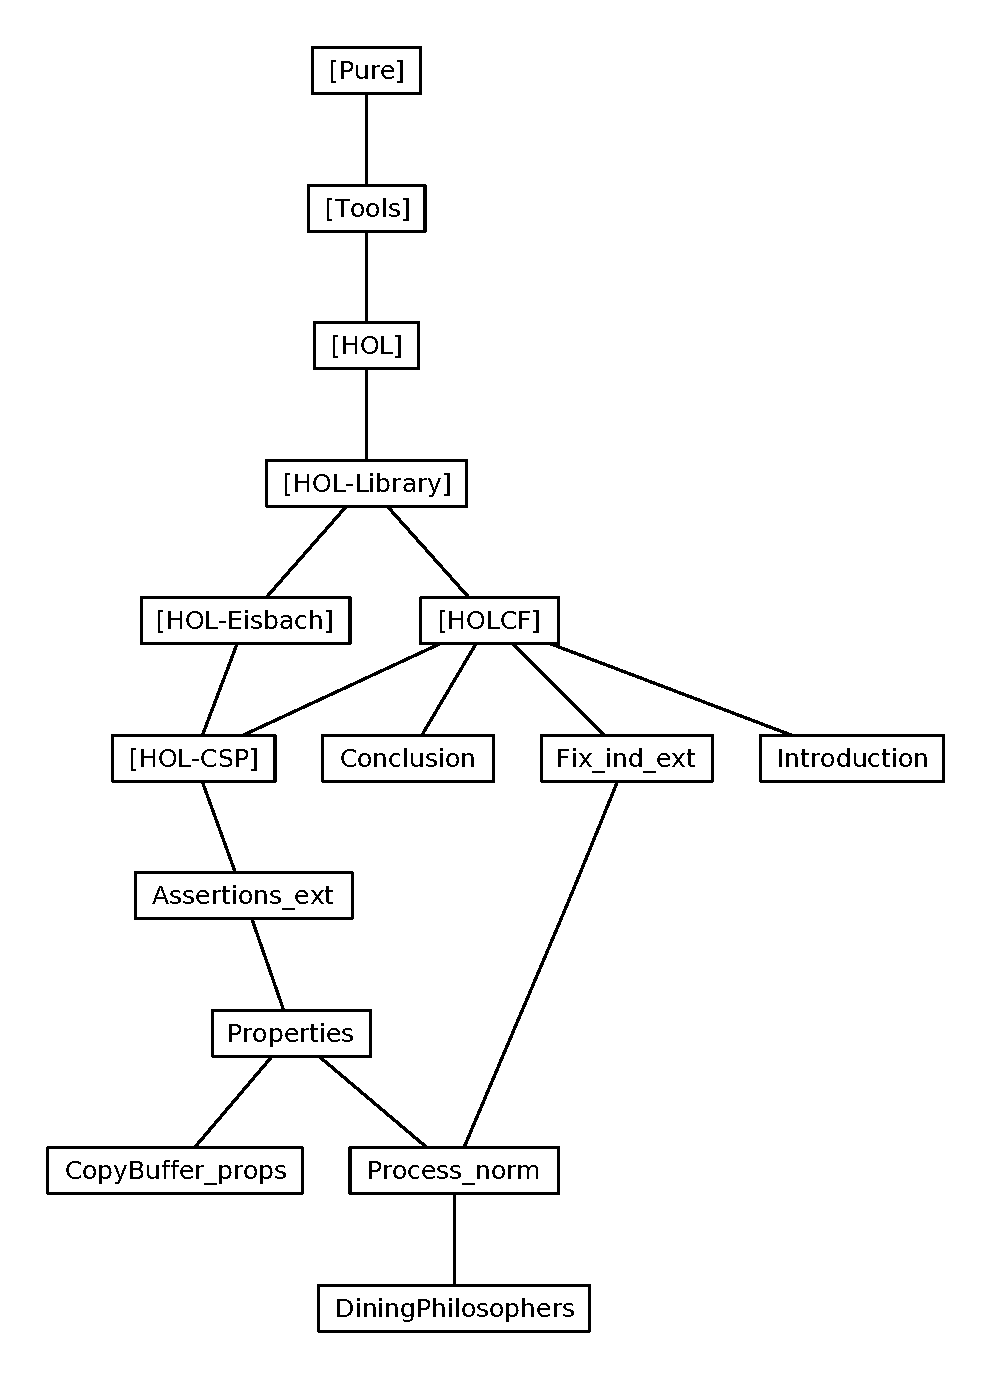
\includegraphics[width=\textwidth]{session_graph}
\end{center}
\caption{Theory Dependency Graph\label{theory-deps}}
\end{figure}

% sane default for proof documents
\parindent 0pt\parskip 0.5ex

% generated text of all theories
\clearpage
%
\begin{isabellebody}%
\setisabellecontext{Value{\isacharunderscore}{\kern0pt}Iteration}%
%
\isadelimtheory
\isanewline
\isanewline
%
\endisadelimtheory
%
\isatagtheory
\isacommand{theory}\isamarkupfalse%
\ Value{\isacharunderscore}{\kern0pt}Iteration\isanewline
\ \ \isakeyword{imports}\ {\isachardoublequoteopen}MDP{\isacharminus}{\kern0pt}Rewards{\isachardot}{\kern0pt}MDP{\isacharunderscore}{\kern0pt}reward{\isachardoublequoteclose}\isanewline
\isakeyword{begin}%
\endisatagtheory
{\isafoldtheory}%
%
\isadelimtheory
\isanewline
%
\endisadelimtheory
\isanewline
\isacommand{context}\isamarkupfalse%
\ MDP{\isacharunderscore}{\kern0pt}att{\isacharunderscore}{\kern0pt}{\isasymL}\isanewline
\isakeyword{begin}%
\isadelimdocument
%
\endisadelimdocument
%
\isatagdocument
%
\isamarkupsection{Value Iteration%
}
\isamarkuptrue%
%
\endisatagdocument
{\isafolddocument}%
%
\isadelimdocument
%
\endisadelimdocument
%
\begin{isamarkuptext}%
In the previous sections we derived that repeated application of \isa{{\isasymL}\isactrlsub b} to any bounded 
function from states to the reals converges to the optimal value of the MDP \isa{{\isasymnu}\isactrlsub b{\isacharunderscore}{\kern0pt}opt}.

We can turn this procedure into an algorithm that computes not only an approximation of 
\isa{{\isasymnu}\isactrlsub b{\isacharunderscore}{\kern0pt}opt} but also a policy that is arbitrarily close to optimal.

Most of the proofs rely on the assumption that the supremum in \isa{{\isasymL}\isactrlsub b} can always be attained.%
\end{isamarkuptext}\isamarkuptrue%
%
\begin{isamarkuptext}%
The following lemma shows that the relation we use to prove termination of the value iteration 
algorithm decreases in each step.
In essence, the distance of the estimate to the optimal value decreases by a factor of at 
least \isa{l} per iteration.%
\end{isamarkuptext}\isamarkuptrue%
\isacommand{lemma}\isamarkupfalse%
\ vi{\isacharunderscore}{\kern0pt}rel{\isacharunderscore}{\kern0pt}dec{\isacharcolon}{\kern0pt}\ \isanewline
\ \ \isakeyword{assumes}\ {\isachardoublequoteopen}l\ {\isasymnoteq}\ {\isadigit{0}}{\isachardoublequoteclose}\ {\isachardoublequoteopen}{\isasymL}\isactrlsub b\ v\ {\isasymnoteq}\ {\isasymnu}\isactrlsub b{\isacharunderscore}{\kern0pt}opt{\isachardoublequoteclose}\isanewline
\ \ \isakeyword{shows}\ {\isachardoublequoteopen}{\isasymlceil}log\ {\isacharparenleft}{\kern0pt}{\isadigit{1}}\ {\isacharslash}{\kern0pt}\ l{\isacharparenright}{\kern0pt}\ {\isacharparenleft}{\kern0pt}dist\ {\isacharparenleft}{\kern0pt}{\isasymL}\isactrlsub b\ v{\isacharparenright}{\kern0pt}\ {\isasymnu}\isactrlsub b{\isacharunderscore}{\kern0pt}opt{\isacharparenright}{\kern0pt}\ {\isacharminus}{\kern0pt}\ c{\isasymrceil}\ {\isacharless}{\kern0pt}\ {\isasymlceil}log\ {\isacharparenleft}{\kern0pt}{\isadigit{1}}\ {\isacharslash}{\kern0pt}\ l{\isacharparenright}{\kern0pt}\ {\isacharparenleft}{\kern0pt}dist\ v\ {\isasymnu}\isactrlsub b{\isacharunderscore}{\kern0pt}opt{\isacharparenright}{\kern0pt}\ {\isacharminus}{\kern0pt}\ c{\isasymrceil}{\isachardoublequoteclose}\isanewline
%
\isadelimproof
%
\endisadelimproof
%
\isatagproof
\isacommand{proof}\isamarkupfalse%
\ {\isacharminus}{\kern0pt}\isanewline
\ \ \isacommand{have}\isamarkupfalse%
\ {\isachardoublequoteopen}log\ {\isacharparenleft}{\kern0pt}{\isadigit{1}}\ {\isacharslash}{\kern0pt}\ l{\isacharparenright}{\kern0pt}\ {\isacharparenleft}{\kern0pt}dist\ {\isacharparenleft}{\kern0pt}{\isasymL}\isactrlsub b\ v{\isacharparenright}{\kern0pt}\ {\isasymnu}\isactrlsub b{\isacharunderscore}{\kern0pt}opt{\isacharparenright}{\kern0pt}\ {\isacharminus}{\kern0pt}\ c\ {\isasymle}\ log\ {\isacharparenleft}{\kern0pt}{\isadigit{1}}\ {\isacharslash}{\kern0pt}\ l{\isacharparenright}{\kern0pt}\ {\isacharparenleft}{\kern0pt}l\ {\isacharasterisk}{\kern0pt}\ dist\ v\ {\isasymnu}\isactrlsub b{\isacharunderscore}{\kern0pt}opt{\isacharparenright}{\kern0pt}\ {\isacharminus}{\kern0pt}\ c{\isachardoublequoteclose}\isanewline
\ \ \ \ \isacommand{using}\isamarkupfalse%
\ contraction{\isacharunderscore}{\kern0pt}{\isasymL}{\isacharbrackleft}{\kern0pt}of\ {\isacharunderscore}{\kern0pt}\ {\isachardoublequoteopen}{\isasymnu}\isactrlsub b{\isacharunderscore}{\kern0pt}opt{\isachardoublequoteclose}{\isacharbrackright}{\kern0pt}\ disc{\isacharunderscore}{\kern0pt}lt{\isacharunderscore}{\kern0pt}one\isanewline
\ \ \ \ \isacommand{by}\isamarkupfalse%
\ {\isacharparenleft}{\kern0pt}auto\ simp{\isacharcolon}{\kern0pt}\ assms\ less{\isacharunderscore}{\kern0pt}le\ intro{\isacharcolon}{\kern0pt}\ log{\isacharunderscore}{\kern0pt}le{\isacharparenright}{\kern0pt}\isanewline
\ \ \isacommand{also}\isamarkupfalse%
\ \isacommand{have}\isamarkupfalse%
\ {\isachardoublequoteopen}{\isasymdots}\ {\isacharequal}{\kern0pt}\ log\ {\isacharparenleft}{\kern0pt}{\isadigit{1}}\ {\isacharslash}{\kern0pt}\ l{\isacharparenright}{\kern0pt}\ l\ {\isacharplus}{\kern0pt}\ log\ {\isacharparenleft}{\kern0pt}{\isadigit{1}}{\isacharslash}{\kern0pt}l{\isacharparenright}{\kern0pt}\ {\isacharparenleft}{\kern0pt}dist\ v\ {\isasymnu}\isactrlsub b{\isacharunderscore}{\kern0pt}opt{\isacharparenright}{\kern0pt}\ {\isacharminus}{\kern0pt}\ c{\isachardoublequoteclose}\isanewline
\ \ \ \ \isacommand{using}\isamarkupfalse%
\ assms\ disc{\isacharunderscore}{\kern0pt}lt{\isacharunderscore}{\kern0pt}one\ \isanewline
\ \ \ \ \isacommand{by}\isamarkupfalse%
\ {\isacharparenleft}{\kern0pt}auto\ simp{\isacharcolon}{\kern0pt}\ less{\isacharunderscore}{\kern0pt}le\ intro{\isacharbang}{\kern0pt}{\isacharcolon}{\kern0pt}\ log{\isacharunderscore}{\kern0pt}mult{\isacharparenright}{\kern0pt}\isanewline
\ \ \isacommand{also}\isamarkupfalse%
\ \isacommand{have}\isamarkupfalse%
\ {\isachardoublequoteopen}{\isasymdots}\ {\isacharequal}{\kern0pt}\ {\isacharminus}{\kern0pt}{\isacharparenleft}{\kern0pt}log\ {\isacharparenleft}{\kern0pt}{\isadigit{1}}\ {\isacharslash}{\kern0pt}\ l{\isacharparenright}{\kern0pt}\ {\isacharparenleft}{\kern0pt}{\isadigit{1}}{\isacharslash}{\kern0pt}l{\isacharparenright}{\kern0pt}{\isacharparenright}{\kern0pt}\ {\isacharplus}{\kern0pt}\ {\isacharparenleft}{\kern0pt}log\ {\isacharparenleft}{\kern0pt}{\isadigit{1}}{\isacharslash}{\kern0pt}l{\isacharparenright}{\kern0pt}\ {\isacharparenleft}{\kern0pt}dist\ v\ {\isasymnu}\isactrlsub b{\isacharunderscore}{\kern0pt}opt{\isacharparenright}{\kern0pt}{\isacharparenright}{\kern0pt}\ {\isacharminus}{\kern0pt}\ c{\isachardoublequoteclose}\isanewline
\ \ \ \ \isacommand{using}\isamarkupfalse%
\ assms\ disc{\isacharunderscore}{\kern0pt}lt{\isacharunderscore}{\kern0pt}one\isanewline
\ \ \ \ \isacommand{by}\isamarkupfalse%
\ {\isacharparenleft}{\kern0pt}subst\ log{\isacharunderscore}{\kern0pt}inverse{\isacharbrackleft}{\kern0pt}symmetric{\isacharbrackright}{\kern0pt}{\isacharparenright}{\kern0pt}\ {\isacharparenleft}{\kern0pt}auto\ simp{\isacharcolon}{\kern0pt}\ less{\isacharunderscore}{\kern0pt}le\ right{\isacharunderscore}{\kern0pt}inverse{\isacharunderscore}{\kern0pt}eq{\isacharparenright}{\kern0pt}\isanewline
\ \ \isacommand{also}\isamarkupfalse%
\ \isacommand{have}\isamarkupfalse%
\ {\isachardoublequoteopen}{\isasymdots}\ {\isacharequal}{\kern0pt}\ {\isacharparenleft}{\kern0pt}log\ {\isacharparenleft}{\kern0pt}{\isadigit{1}}{\isacharslash}{\kern0pt}l{\isacharparenright}{\kern0pt}\ {\isacharparenleft}{\kern0pt}dist\ v\ {\isasymnu}\isactrlsub b{\isacharunderscore}{\kern0pt}opt{\isacharparenright}{\kern0pt}{\isacharparenright}{\kern0pt}\ {\isacharminus}{\kern0pt}\ {\isadigit{1}}\ {\isacharminus}{\kern0pt}\ c{\isachardoublequoteclose}\isanewline
\ \ \ \ \isacommand{using}\isamarkupfalse%
\ assms\ order{\isachardot}{\kern0pt}strict{\isacharunderscore}{\kern0pt}implies{\isacharunderscore}{\kern0pt}not{\isacharunderscore}{\kern0pt}eq{\isacharbrackleft}{\kern0pt}OF\ disc{\isacharunderscore}{\kern0pt}lt{\isacharunderscore}{\kern0pt}one{\isacharbrackright}{\kern0pt}\isanewline
\ \ \ \ \isacommand{by}\isamarkupfalse%
\ {\isacharparenleft}{\kern0pt}auto\ intro{\isacharbang}{\kern0pt}{\isacharcolon}{\kern0pt}\ log{\isacharunderscore}{\kern0pt}eq{\isacharunderscore}{\kern0pt}one\ neq{\isacharunderscore}{\kern0pt}le{\isacharunderscore}{\kern0pt}trans{\isacharparenright}{\kern0pt}\isanewline
\ \ \isacommand{finally}\isamarkupfalse%
\ \isacommand{have}\isamarkupfalse%
\ {\isachardoublequoteopen}log\ {\isacharparenleft}{\kern0pt}{\isadigit{1}}\ {\isacharslash}{\kern0pt}\ l{\isacharparenright}{\kern0pt}\ {\isacharparenleft}{\kern0pt}dist\ {\isacharparenleft}{\kern0pt}{\isasymL}\isactrlsub b\ v{\isacharparenright}{\kern0pt}\ {\isasymnu}\isactrlsub b{\isacharunderscore}{\kern0pt}opt{\isacharparenright}{\kern0pt}\ {\isacharminus}{\kern0pt}\ c\ {\isasymle}\ log\ {\isacharparenleft}{\kern0pt}{\isadigit{1}}\ {\isacharslash}{\kern0pt}\ l{\isacharparenright}{\kern0pt}\ {\isacharparenleft}{\kern0pt}dist\ v\ {\isasymnu}\isactrlsub b{\isacharunderscore}{\kern0pt}opt{\isacharparenright}{\kern0pt}\ {\isacharminus}{\kern0pt}\ {\isadigit{1}}\ {\isacharminus}{\kern0pt}\ c{\isachardoublequoteclose}\ \isacommand{{\isachardot}{\kern0pt}}\isamarkupfalse%
\isanewline
\ \ \isacommand{thus}\isamarkupfalse%
\ {\isacharquery}{\kern0pt}thesis\isanewline
\ \ \ \ \isacommand{by}\isamarkupfalse%
\ linarith\isanewline
\isacommand{qed}\isamarkupfalse%
%
\endisatagproof
{\isafoldproof}%
%
\isadelimproof
\isanewline
%
\endisadelimproof
\isanewline
\isacommand{lemma}\isamarkupfalse%
\ dist{\isacharunderscore}{\kern0pt}{\isasymL}\isactrlsub b{\isacharunderscore}{\kern0pt}lt{\isacharunderscore}{\kern0pt}dist{\isacharunderscore}{\kern0pt}opt{\isacharcolon}{\kern0pt}\ {\isachardoublequoteopen}dist\ v\ {\isacharparenleft}{\kern0pt}{\isasymL}\isactrlsub b\ v{\isacharparenright}{\kern0pt}\ {\isasymle}\ {\isadigit{2}}\ {\isacharasterisk}{\kern0pt}\ dist\ v\ {\isasymnu}\isactrlsub b{\isacharunderscore}{\kern0pt}opt{\isachardoublequoteclose}\isanewline
%
\isadelimproof
%
\endisadelimproof
%
\isatagproof
\isacommand{proof}\isamarkupfalse%
\ {\isacharminus}{\kern0pt}\isanewline
\ \ \isacommand{have}\isamarkupfalse%
\ le{\isadigit{1}}{\isacharcolon}{\kern0pt}\ {\isachardoublequoteopen}dist\ v\ {\isacharparenleft}{\kern0pt}{\isasymL}\isactrlsub b\ v{\isacharparenright}{\kern0pt}\ {\isasymle}\ dist\ v\ {\isasymnu}\isactrlsub b{\isacharunderscore}{\kern0pt}opt\ {\isacharplus}{\kern0pt}\ dist\ {\isacharparenleft}{\kern0pt}{\isasymL}\isactrlsub b\ v{\isacharparenright}{\kern0pt}\ {\isasymnu}\isactrlsub b{\isacharunderscore}{\kern0pt}opt{\isachardoublequoteclose}\isanewline
\ \ \ \ \isacommand{by}\isamarkupfalse%
\ {\isacharparenleft}{\kern0pt}simp\ add{\isacharcolon}{\kern0pt}\ dist{\isacharunderscore}{\kern0pt}triangle\ dist{\isacharunderscore}{\kern0pt}commute{\isacharparenright}{\kern0pt}\isanewline
\ \ \isacommand{have}\isamarkupfalse%
\ le{\isadigit{2}}{\isacharcolon}{\kern0pt}\ {\isachardoublequoteopen}dist\ {\isacharparenleft}{\kern0pt}{\isasymL}\isactrlsub b\ v{\isacharparenright}{\kern0pt}\ {\isasymnu}\isactrlsub b{\isacharunderscore}{\kern0pt}opt\ {\isasymle}\ l\ {\isacharasterisk}{\kern0pt}\ dist\ v\ {\isasymnu}\isactrlsub b{\isacharunderscore}{\kern0pt}opt{\isachardoublequoteclose}\isanewline
\ \ \ \ \isacommand{using}\isamarkupfalse%
\ {\isasymL}\isactrlsub b{\isacharunderscore}{\kern0pt}opt\ contraction{\isacharunderscore}{\kern0pt}{\isasymL}\isanewline
\ \ \ \ \isacommand{by}\isamarkupfalse%
\ metis\isanewline
\ \ \isacommand{show}\isamarkupfalse%
\ {\isacharquery}{\kern0pt}thesis\isanewline
\ \ \ \ \isacommand{using}\isamarkupfalse%
\ mult{\isacharunderscore}{\kern0pt}right{\isacharunderscore}{\kern0pt}mono{\isacharbrackleft}{\kern0pt}of\ l\ {\isadigit{1}}{\isacharbrackright}{\kern0pt}\ disc{\isacharunderscore}{\kern0pt}lt{\isacharunderscore}{\kern0pt}one\ \isanewline
\ \ \ \ \isacommand{by}\isamarkupfalse%
\ {\isacharparenleft}{\kern0pt}fastforce\ intro{\isacharbang}{\kern0pt}{\isacharcolon}{\kern0pt}\ order{\isachardot}{\kern0pt}trans{\isacharbrackleft}{\kern0pt}OF\ le{\isadigit{2}}{\isacharbrackright}{\kern0pt}\ order{\isachardot}{\kern0pt}trans{\isacharbrackleft}{\kern0pt}OF\ le{\isadigit{1}}{\isacharbrackright}{\kern0pt}{\isacharparenright}{\kern0pt}\isanewline
\isacommand{qed}\isamarkupfalse%
%
\endisatagproof
{\isafoldproof}%
%
\isadelimproof
\isanewline
%
\endisadelimproof
\isanewline
\isacommand{abbreviation}\isamarkupfalse%
\ {\isachardoublequoteopen}term{\isacharunderscore}{\kern0pt}measure\ {\isasymequiv}\ {\isacharparenleft}{\kern0pt}{\isasymlambda}{\isacharparenleft}{\kern0pt}eps{\isacharcomma}{\kern0pt}\ v{\isacharparenright}{\kern0pt}{\isachardot}{\kern0pt}\isanewline
\ \ \ \ if\ v\ {\isacharequal}{\kern0pt}\ {\isasymnu}\isactrlsub b{\isacharunderscore}{\kern0pt}opt\ {\isasymor}\ l\ {\isacharequal}{\kern0pt}\ {\isadigit{0}}\isanewline
\ \ \ \ then\ {\isadigit{0}}\isanewline
\ \ \ \ else\ nat\ {\isacharparenleft}{\kern0pt}ceiling\ {\isacharparenleft}{\kern0pt}log\ {\isacharparenleft}{\kern0pt}{\isadigit{1}}{\isacharslash}{\kern0pt}l{\isacharparenright}{\kern0pt}\ {\isacharparenleft}{\kern0pt}dist\ v\ {\isasymnu}\isactrlsub b{\isacharunderscore}{\kern0pt}opt{\isacharparenright}{\kern0pt}\ {\isacharminus}{\kern0pt}\ log\ {\isacharparenleft}{\kern0pt}{\isadigit{1}}{\isacharslash}{\kern0pt}l{\isacharparenright}{\kern0pt}\ {\isacharparenleft}{\kern0pt}eps\ {\isacharasterisk}{\kern0pt}\ {\isacharparenleft}{\kern0pt}{\isadigit{1}}{\isacharminus}{\kern0pt}l{\isacharparenright}{\kern0pt}\ {\isacharslash}{\kern0pt}\ {\isacharparenleft}{\kern0pt}{\isadigit{8}}\ {\isacharasterisk}{\kern0pt}\ l{\isacharparenright}{\kern0pt}{\isacharparenright}{\kern0pt}{\isacharparenright}{\kern0pt}{\isacharparenright}{\kern0pt}{\isacharparenright}{\kern0pt}{\isachardoublequoteclose}\isanewline
\isanewline
\isacommand{function}\isamarkupfalse%
\ value{\isacharunderscore}{\kern0pt}iteration\ {\isacharcolon}{\kern0pt}{\isacharcolon}{\kern0pt}\ {\isachardoublequoteopen}real\ {\isasymRightarrow}\ {\isacharparenleft}{\kern0pt}{\isacharprime}{\kern0pt}s\ {\isasymRightarrow}\isactrlsub b\ real{\isacharparenright}{\kern0pt}\ {\isasymRightarrow}\ {\isacharparenleft}{\kern0pt}{\isacharprime}{\kern0pt}s\ {\isasymRightarrow}\isactrlsub b\ real{\isacharparenright}{\kern0pt}{\isachardoublequoteclose}\ \isakeyword{where}\isanewline
\ \ {\isachardoublequoteopen}value{\isacharunderscore}{\kern0pt}iteration\ eps\ v\ {\isacharequal}{\kern0pt}\isanewline
\ \ {\isacharparenleft}{\kern0pt}if\ {\isadigit{2}}\ {\isacharasterisk}{\kern0pt}\ l\ {\isacharasterisk}{\kern0pt}\ dist\ v\ {\isacharparenleft}{\kern0pt}{\isasymL}\isactrlsub b\ v{\isacharparenright}{\kern0pt}\ {\isacharless}{\kern0pt}\ eps\ {\isacharasterisk}{\kern0pt}\ {\isacharparenleft}{\kern0pt}{\isadigit{1}}{\isacharminus}{\kern0pt}l{\isacharparenright}{\kern0pt}\ {\isasymor}\ eps\ {\isasymle}\ {\isadigit{0}}\ then\ {\isasymL}\isactrlsub b\ v\ else\ value{\isacharunderscore}{\kern0pt}iteration\ eps\ {\isacharparenleft}{\kern0pt}{\isasymL}\isactrlsub b\ v{\isacharparenright}{\kern0pt}{\isacharparenright}{\kern0pt}{\isachardoublequoteclose}\isanewline
%
\isadelimproof
\ \ %
\endisadelimproof
%
\isatagproof
\isacommand{by}\isamarkupfalse%
\ auto%
\endisatagproof
{\isafoldproof}%
%
\isadelimproof
\isanewline
%
\endisadelimproof
\isanewline
\isacommand{termination}\isamarkupfalse%
\isanewline
%
\isadelimproof
%
\endisadelimproof
%
\isatagproof
\isacommand{proof}\isamarkupfalse%
\ {\isacharparenleft}{\kern0pt}relation\ {\isachardoublequoteopen}Wellfounded{\isachardot}{\kern0pt}measure\ term{\isacharunderscore}{\kern0pt}measure{\isachardoublequoteclose}{\isacharcomma}{\kern0pt}\ {\isacharparenleft}{\kern0pt}simp{\isacharsemicolon}{\kern0pt}\ fail{\isacharparenright}{\kern0pt}{\isacharcomma}{\kern0pt}\ cases\ {\isachardoublequoteopen}l\ {\isacharequal}{\kern0pt}\ {\isadigit{0}}{\isachardoublequoteclose}{\isacharparenright}{\kern0pt}\isanewline
\ \ \isacommand{case}\isamarkupfalse%
\ False\isanewline
\ \ \isacommand{fix}\isamarkupfalse%
\ eps\ v\isanewline
\ \ \isacommand{assume}\isamarkupfalse%
\ h{\isacharcolon}{\kern0pt}\ {\isachardoublequoteopen}{\isasymnot}\ {\isacharparenleft}{\kern0pt}{\isadigit{2}}\ {\isacharasterisk}{\kern0pt}\ l\ {\isacharasterisk}{\kern0pt}\ dist\ v\ {\isacharparenleft}{\kern0pt}{\isasymL}\isactrlsub b\ v{\isacharparenright}{\kern0pt}\ {\isacharless}{\kern0pt}\ eps\ {\isacharasterisk}{\kern0pt}\ {\isacharparenleft}{\kern0pt}{\isadigit{1}}\ {\isacharminus}{\kern0pt}\ l{\isacharparenright}{\kern0pt}\ {\isasymor}\ eps\ {\isasymle}\ {\isadigit{0}}{\isacharparenright}{\kern0pt}{\isachardoublequoteclose}\isanewline
\ \ \isacommand{show}\isamarkupfalse%
\ {\isachardoublequoteopen}{\isacharparenleft}{\kern0pt}{\isacharparenleft}{\kern0pt}eps{\isacharcomma}{\kern0pt}\ {\isasymL}\isactrlsub b\ v{\isacharparenright}{\kern0pt}{\isacharcomma}{\kern0pt}\ eps{\isacharcomma}{\kern0pt}\ v{\isacharparenright}{\kern0pt}\ {\isasymin}\ Wellfounded{\isachardot}{\kern0pt}measure\ term{\isacharunderscore}{\kern0pt}measure{\isachardoublequoteclose}\isanewline
\ \ \isacommand{proof}\isamarkupfalse%
\ {\isacharminus}{\kern0pt}\isanewline
\ \ \ \ \isacommand{have}\isamarkupfalse%
\ gt{\isacharunderscore}{\kern0pt}zero{\isacharbrackleft}{\kern0pt}simp{\isacharbrackright}{\kern0pt}{\isacharcolon}{\kern0pt}\ {\isachardoublequoteopen}l\ {\isasymnoteq}\ {\isadigit{0}}{\isachardoublequoteclose}\ {\isachardoublequoteopen}eps\ {\isachargreater}{\kern0pt}\ {\isadigit{0}}{\isachardoublequoteclose}\ \isakeyword{and}\ dist{\isacharunderscore}{\kern0pt}ge{\isacharcolon}{\kern0pt}\ {\isachardoublequoteopen}eps\ {\isacharasterisk}{\kern0pt}\ {\isacharparenleft}{\kern0pt}{\isadigit{1}}\ {\isacharminus}{\kern0pt}\ l{\isacharparenright}{\kern0pt}\ {\isasymle}\ dist\ v\ {\isacharparenleft}{\kern0pt}{\isasymL}\isactrlsub b\ v{\isacharparenright}{\kern0pt}\ {\isacharasterisk}{\kern0pt}\ {\isacharparenleft}{\kern0pt}{\isadigit{2}}\ {\isacharasterisk}{\kern0pt}\ l{\isacharparenright}{\kern0pt}{\isachardoublequoteclose}\isanewline
\ \ \ \ \ \ \isacommand{using}\isamarkupfalse%
\ h\isanewline
\ \ \ \ \ \ \isacommand{by}\isamarkupfalse%
\ {\isacharparenleft}{\kern0pt}auto\ simp{\isacharcolon}{\kern0pt}\ algebra{\isacharunderscore}{\kern0pt}simps{\isacharparenright}{\kern0pt}\isanewline
\ \ \ \ \isacommand{have}\isamarkupfalse%
\ v{\isacharunderscore}{\kern0pt}not{\isacharunderscore}{\kern0pt}opt{\isacharcolon}{\kern0pt}\ {\isachardoublequoteopen}v\ {\isasymnoteq}\ {\isasymnu}\isactrlsub b{\isacharunderscore}{\kern0pt}opt{\isachardoublequoteclose}\isanewline
\ \ \ \ \ \ \isacommand{using}\isamarkupfalse%
\ h\isanewline
\ \ \ \ \ \ \isacommand{by}\isamarkupfalse%
\ force\isanewline
\ \ \ \ \isacommand{have}\isamarkupfalse%
\ {\isachardoublequoteopen}log\ {\isacharparenleft}{\kern0pt}{\isadigit{1}}\ {\isacharslash}{\kern0pt}\ l{\isacharparenright}{\kern0pt}\ {\isacharparenleft}{\kern0pt}eps\ {\isacharasterisk}{\kern0pt}\ {\isacharparenleft}{\kern0pt}{\isadigit{1}}\ {\isacharminus}{\kern0pt}\ l{\isacharparenright}{\kern0pt}\ {\isacharslash}{\kern0pt}\ {\isacharparenleft}{\kern0pt}{\isadigit{8}}\ {\isacharasterisk}{\kern0pt}\ l{\isacharparenright}{\kern0pt}{\isacharparenright}{\kern0pt}\ {\isacharless}{\kern0pt}\ log\ {\isacharparenleft}{\kern0pt}{\isadigit{1}}\ {\isacharslash}{\kern0pt}\ l{\isacharparenright}{\kern0pt}\ {\isacharparenleft}{\kern0pt}dist\ v\ {\isasymnu}\isactrlsub b{\isacharunderscore}{\kern0pt}opt{\isacharparenright}{\kern0pt}{\isachardoublequoteclose}\isanewline
\ \ \ \ \isacommand{proof}\isamarkupfalse%
\ {\isacharparenleft}{\kern0pt}intro\ log{\isacharunderscore}{\kern0pt}less{\isacharparenright}{\kern0pt}\isanewline
\ \ \ \ \ \ \isacommand{show}\isamarkupfalse%
\ {\isachardoublequoteopen}{\isadigit{1}}\ {\isacharless}{\kern0pt}\ {\isadigit{1}}\ {\isacharslash}{\kern0pt}\ l{\isachardoublequoteclose}\isanewline
\ \ \ \ \ \ \ \ \isacommand{by}\isamarkupfalse%
\ {\isacharparenleft}{\kern0pt}auto\ intro{\isacharbang}{\kern0pt}{\isacharcolon}{\kern0pt}\ mult{\isacharunderscore}{\kern0pt}imp{\isacharunderscore}{\kern0pt}less{\isacharunderscore}{\kern0pt}div{\isacharunderscore}{\kern0pt}pos\ intro{\isacharcolon}{\kern0pt}\ neq{\isacharunderscore}{\kern0pt}le{\isacharunderscore}{\kern0pt}trans{\isacharparenright}{\kern0pt}\isanewline
\ \ \ \ \ \ \isacommand{show}\isamarkupfalse%
\ {\isachardoublequoteopen}{\isadigit{0}}\ {\isacharless}{\kern0pt}\ eps\ {\isacharasterisk}{\kern0pt}\ {\isacharparenleft}{\kern0pt}{\isadigit{1}}\ {\isacharminus}{\kern0pt}\ l{\isacharparenright}{\kern0pt}\ {\isacharslash}{\kern0pt}\ {\isacharparenleft}{\kern0pt}{\isadigit{8}}\ {\isacharasterisk}{\kern0pt}\ l{\isacharparenright}{\kern0pt}{\isachardoublequoteclose}\ \isanewline
\ \ \ \ \ \ \ \ \isacommand{by}\isamarkupfalse%
\ {\isacharparenleft}{\kern0pt}auto\ intro{\isacharbang}{\kern0pt}{\isacharcolon}{\kern0pt}\ mult{\isacharunderscore}{\kern0pt}imp{\isacharunderscore}{\kern0pt}less{\isacharunderscore}{\kern0pt}div{\isacharunderscore}{\kern0pt}pos\ intro{\isacharcolon}{\kern0pt}\ neq{\isacharunderscore}{\kern0pt}le{\isacharunderscore}{\kern0pt}trans{\isacharparenright}{\kern0pt}\isanewline
\ \ \ \ \ \ \isacommand{show}\isamarkupfalse%
\ {\isachardoublequoteopen}eps\ {\isacharasterisk}{\kern0pt}\ {\isacharparenleft}{\kern0pt}{\isadigit{1}}\ {\isacharminus}{\kern0pt}\ l{\isacharparenright}{\kern0pt}\ {\isacharslash}{\kern0pt}\ {\isacharparenleft}{\kern0pt}{\isadigit{8}}\ {\isacharasterisk}{\kern0pt}\ l{\isacharparenright}{\kern0pt}\ {\isacharless}{\kern0pt}\ dist\ v\ {\isasymnu}\isactrlsub b{\isacharunderscore}{\kern0pt}opt{\isachardoublequoteclose}\ \isanewline
\ \ \ \ \ \ \ \ \isacommand{using}\isamarkupfalse%
\ dist{\isacharunderscore}{\kern0pt}pos{\isacharunderscore}{\kern0pt}lt{\isacharbrackleft}{\kern0pt}OF\ v{\isacharunderscore}{\kern0pt}not{\isacharunderscore}{\kern0pt}opt{\isacharbrackright}{\kern0pt}\ dist{\isacharunderscore}{\kern0pt}{\isasymL}\isactrlsub b{\isacharunderscore}{\kern0pt}lt{\isacharunderscore}{\kern0pt}dist{\isacharunderscore}{\kern0pt}opt{\isacharbrackleft}{\kern0pt}of\ v{\isacharbrackright}{\kern0pt}\ gt{\isacharunderscore}{\kern0pt}zero\ zero{\isacharunderscore}{\kern0pt}le{\isacharunderscore}{\kern0pt}disc\ \isanewline
\ \ \ \ \ \ \ \ \ \ mult{\isacharunderscore}{\kern0pt}strict{\isacharunderscore}{\kern0pt}left{\isacharunderscore}{\kern0pt}mono{\isacharbrackleft}{\kern0pt}of\ {\isachardoublequoteopen}dist\ v\ {\isacharparenleft}{\kern0pt}{\isasymL}\isactrlsub b\ v{\isacharparenright}{\kern0pt}{\isachardoublequoteclose}\ {\isachardoublequoteopen}{\isacharparenleft}{\kern0pt}{\isadigit{4}}\ {\isacharasterisk}{\kern0pt}\ dist\ v\ {\isasymnu}\isactrlsub b{\isacharunderscore}{\kern0pt}opt{\isacharparenright}{\kern0pt}{\isachardoublequoteclose}\ l{\isacharbrackright}{\kern0pt}\isanewline
\ \ \ \ \ \ \ \ \isacommand{by}\isamarkupfalse%
\ {\isacharparenleft}{\kern0pt}intro\ mult{\isacharunderscore}{\kern0pt}imp{\isacharunderscore}{\kern0pt}div{\isacharunderscore}{\kern0pt}pos{\isacharunderscore}{\kern0pt}less\ le{\isacharunderscore}{\kern0pt}less{\isacharunderscore}{\kern0pt}trans{\isacharbrackleft}{\kern0pt}OF\ dist{\isacharunderscore}{\kern0pt}ge{\isacharbrackright}{\kern0pt}{\isacharcomma}{\kern0pt}\ argo{\isacharplus}{\kern0pt}{\isacharparenright}{\kern0pt}\isanewline
\ \ \ \ \isacommand{qed}\isamarkupfalse%
\isanewline
\ \ \ \ \isacommand{thus}\isamarkupfalse%
\ {\isacharquery}{\kern0pt}thesis\isanewline
\ \ \ \ \ \ \isacommand{using}\isamarkupfalse%
\ vi{\isacharunderscore}{\kern0pt}rel{\isacharunderscore}{\kern0pt}dec\ h\isanewline
\ \ \ \ \ \ \isacommand{by}\isamarkupfalse%
\ auto\isanewline
\ \ \isacommand{qed}\isamarkupfalse%
\isanewline
\isacommand{qed}\isamarkupfalse%
\ auto%
\endisatagproof
{\isafoldproof}%
%
\isadelimproof
%
\endisadelimproof
%
\begin{isamarkuptext}%
The distance between an estimate for the value and the optimal value can be bounded with respect to 
the distance between the estimate and the result of applying it to \isa{{\isasymL}\isactrlsub b}%
\end{isamarkuptext}\isamarkuptrue%
\isacommand{lemma}\isamarkupfalse%
\ contraction{\isacharunderscore}{\kern0pt}{\isasymL}{\isacharunderscore}{\kern0pt}dist{\isacharcolon}{\kern0pt}\ {\isachardoublequoteopen}{\isacharparenleft}{\kern0pt}{\isadigit{1}}\ {\isacharminus}{\kern0pt}\ l{\isacharparenright}{\kern0pt}\ {\isacharasterisk}{\kern0pt}\ dist\ v\ {\isasymnu}\isactrlsub b{\isacharunderscore}{\kern0pt}opt\ {\isasymle}\ dist\ v\ {\isacharparenleft}{\kern0pt}{\isasymL}\isactrlsub b\ v{\isacharparenright}{\kern0pt}{\isachardoublequoteclose}\isanewline
%
\isadelimproof
\ \ %
\endisadelimproof
%
\isatagproof
\isacommand{using}\isamarkupfalse%
\ contraction{\isacharunderscore}{\kern0pt}dist\ contraction{\isacharunderscore}{\kern0pt}{\isasymL}\ disc{\isacharunderscore}{\kern0pt}lt{\isacharunderscore}{\kern0pt}one\ zero{\isacharunderscore}{\kern0pt}le{\isacharunderscore}{\kern0pt}disc\isanewline
\ \ \isacommand{by}\isamarkupfalse%
\ fastforce%
\endisatagproof
{\isafoldproof}%
%
\isadelimproof
\isanewline
%
\endisadelimproof
\isanewline
\isacommand{lemma}\isamarkupfalse%
\ dist{\isacharunderscore}{\kern0pt}{\isasymL}\isactrlsub b{\isacharunderscore}{\kern0pt}opt{\isacharunderscore}{\kern0pt}eps{\isacharcolon}{\kern0pt}\isanewline
\ \ \isakeyword{assumes}\ {\isachardoublequoteopen}eps\ {\isachargreater}{\kern0pt}\ {\isadigit{0}}{\isachardoublequoteclose}\ {\isachardoublequoteopen}{\isadigit{2}}\ {\isacharasterisk}{\kern0pt}\ l\ {\isacharasterisk}{\kern0pt}\ dist\ v\ {\isacharparenleft}{\kern0pt}{\isasymL}\isactrlsub b\ v{\isacharparenright}{\kern0pt}\ {\isacharless}{\kern0pt}\ eps\ {\isacharasterisk}{\kern0pt}\ {\isacharparenleft}{\kern0pt}{\isadigit{1}}{\isacharminus}{\kern0pt}l{\isacharparenright}{\kern0pt}{\isachardoublequoteclose}\isanewline
\ \ \isakeyword{shows}\ {\isachardoublequoteopen}dist\ {\isacharparenleft}{\kern0pt}{\isasymL}\isactrlsub b\ v{\isacharparenright}{\kern0pt}\ {\isasymnu}\isactrlsub b{\isacharunderscore}{\kern0pt}opt\ {\isacharless}{\kern0pt}\ eps\ {\isacharslash}{\kern0pt}\ {\isadigit{2}}{\isachardoublequoteclose}\isanewline
%
\isadelimproof
%
\endisadelimproof
%
\isatagproof
\isacommand{proof}\isamarkupfalse%
\ {\isacharminus}{\kern0pt}\isanewline
\ \ \isacommand{have}\isamarkupfalse%
\ {\isachardoublequoteopen}dist\ v\ {\isasymnu}\isactrlsub b{\isacharunderscore}{\kern0pt}opt\ {\isasymle}\ dist\ v\ {\isacharparenleft}{\kern0pt}{\isasymL}\isactrlsub b\ v{\isacharparenright}{\kern0pt}\ {\isacharslash}{\kern0pt}\ {\isacharparenleft}{\kern0pt}{\isadigit{1}}\ {\isacharminus}{\kern0pt}\ l{\isacharparenright}{\kern0pt}{\isachardoublequoteclose}\isanewline
\ \ \ \ \isacommand{using}\isamarkupfalse%
\ contraction{\isacharunderscore}{\kern0pt}{\isasymL}{\isacharunderscore}{\kern0pt}dist\isanewline
\ \ \ \ \isacommand{by}\isamarkupfalse%
\ {\isacharparenleft}{\kern0pt}simp\ add{\isacharcolon}{\kern0pt}\ mult{\isachardot}{\kern0pt}commute\ pos{\isacharunderscore}{\kern0pt}le{\isacharunderscore}{\kern0pt}divide{\isacharunderscore}{\kern0pt}eq{\isacharparenright}{\kern0pt}\isanewline
\ \ \isacommand{hence}\isamarkupfalse%
\ {\isachardoublequoteopen}{\isadigit{2}}\ {\isacharasterisk}{\kern0pt}\ l\ {\isacharasterisk}{\kern0pt}\ dist\ v\ {\isasymnu}\isactrlsub b{\isacharunderscore}{\kern0pt}opt\ {\isasymle}\ {\isadigit{2}}\ {\isacharasterisk}{\kern0pt}\ l\ {\isacharasterisk}{\kern0pt}\ {\isacharparenleft}{\kern0pt}dist\ v\ {\isacharparenleft}{\kern0pt}{\isasymL}\isactrlsub b\ v{\isacharparenright}{\kern0pt}\ {\isacharslash}{\kern0pt}\ {\isacharparenleft}{\kern0pt}{\isadigit{1}}\ {\isacharminus}{\kern0pt}\ l{\isacharparenright}{\kern0pt}{\isacharparenright}{\kern0pt}{\isachardoublequoteclose}\isanewline
\ \ \ \ \isacommand{using}\isamarkupfalse%
\ contraction{\isacharunderscore}{\kern0pt}{\isasymL}{\isacharunderscore}{\kern0pt}dist\ assms\ mult{\isacharunderscore}{\kern0pt}le{\isacharunderscore}{\kern0pt}cancel{\isacharunderscore}{\kern0pt}left{\isacharunderscore}{\kern0pt}pos{\isacharbrackleft}{\kern0pt}of\ {\isachardoublequoteopen}{\isadigit{2}}\ {\isacharasterisk}{\kern0pt}\ l{\isachardoublequoteclose}{\isacharbrackright}{\kern0pt}\isanewline
\ \ \ \ \isacommand{by}\isamarkupfalse%
\ {\isacharparenleft}{\kern0pt}fastforce\ intro{\isacharbang}{\kern0pt}{\isacharcolon}{\kern0pt}\ mult{\isacharunderscore}{\kern0pt}left{\isacharunderscore}{\kern0pt}mono{\isacharbrackleft}{\kern0pt}of\ {\isacharunderscore}{\kern0pt}\ {\isacharunderscore}{\kern0pt}\ {\isachardoublequoteopen}{\isadigit{2}}\ {\isacharasterisk}{\kern0pt}\ l{\isachardoublequoteclose}{\isacharbrackright}{\kern0pt}{\isacharparenright}{\kern0pt}\isanewline
\ \ \isacommand{hence}\isamarkupfalse%
\ {\isachardoublequoteopen}{\isadigit{2}}\ {\isacharasterisk}{\kern0pt}\ l\ {\isacharasterisk}{\kern0pt}\ dist\ v\ {\isasymnu}\isactrlsub b{\isacharunderscore}{\kern0pt}opt\ {\isacharless}{\kern0pt}\ eps{\isachardoublequoteclose}\isanewline
\ \ \ \ \isacommand{by}\isamarkupfalse%
\ {\isacharparenleft}{\kern0pt}auto\ simp{\isacharcolon}{\kern0pt}\ assms{\isacharparenleft}{\kern0pt}{\isadigit{2}}{\isacharparenright}{\kern0pt}\ pos{\isacharunderscore}{\kern0pt}divide{\isacharunderscore}{\kern0pt}less{\isacharunderscore}{\kern0pt}eq\ intro{\isacharcolon}{\kern0pt}\ order{\isachardot}{\kern0pt}strict{\isacharunderscore}{\kern0pt}trans{\isadigit{1}}{\isacharparenright}{\kern0pt}\isanewline
\ \ \isacommand{hence}\isamarkupfalse%
\ {\isachardoublequoteopen}dist\ v\ {\isasymnu}\isactrlsub b{\isacharunderscore}{\kern0pt}opt\ {\isacharasterisk}{\kern0pt}\ l\ {\isacharless}{\kern0pt}\ eps\ {\isacharslash}{\kern0pt}\ {\isadigit{2}}{\isachardoublequoteclose}\isanewline
\ \ \ \ \isacommand{by}\isamarkupfalse%
\ argo\isanewline
\ \ \isacommand{hence}\isamarkupfalse%
\ {\isachardoublequoteopen}l\ {\isacharasterisk}{\kern0pt}\ dist\ v\ {\isasymnu}\isactrlsub b{\isacharunderscore}{\kern0pt}opt\ {\isacharless}{\kern0pt}\ eps\ {\isacharslash}{\kern0pt}\ {\isadigit{2}}{\isachardoublequoteclose}\isanewline
\ \ \ \ \isacommand{by}\isamarkupfalse%
\ {\isacharparenleft}{\kern0pt}auto\ simp{\isacharcolon}{\kern0pt}\ algebra{\isacharunderscore}{\kern0pt}simps{\isacharparenright}{\kern0pt}\isanewline
\ \ \isacommand{thus}\isamarkupfalse%
\ {\isachardoublequoteopen}dist\ {\isacharparenleft}{\kern0pt}{\isasymL}\isactrlsub b\ v{\isacharparenright}{\kern0pt}\ {\isasymnu}\isactrlsub b{\isacharunderscore}{\kern0pt}opt\ {\isacharless}{\kern0pt}\ eps\ {\isacharslash}{\kern0pt}\ {\isadigit{2}}{\isachardoublequoteclose}\isanewline
\ \ \ \ \isacommand{using}\isamarkupfalse%
\ contraction{\isacharunderscore}{\kern0pt}{\isasymL}{\isacharbrackleft}{\kern0pt}of\ v\ {\isasymnu}\isactrlsub b{\isacharunderscore}{\kern0pt}opt{\isacharbrackright}{\kern0pt}\ \isanewline
\ \ \ \ \isacommand{by}\isamarkupfalse%
\ auto\isanewline
\isacommand{qed}\isamarkupfalse%
%
\endisatagproof
{\isafoldproof}%
%
\isadelimproof
%
\endisadelimproof
%
\begin{isamarkuptext}%
The estimates above allow to give a bound on the error of \isa{value{\isacharunderscore}{\kern0pt}iteration}.%
\end{isamarkuptext}\isamarkuptrue%
\isacommand{declare}\isamarkupfalse%
\ value{\isacharunderscore}{\kern0pt}iteration{\isachardot}{\kern0pt}simps{\isacharbrackleft}{\kern0pt}simp\ del{\isacharbrackright}{\kern0pt}\isanewline
\isanewline
\isacommand{lemma}\isamarkupfalse%
\ value{\isacharunderscore}{\kern0pt}iteration{\isacharunderscore}{\kern0pt}error{\isacharcolon}{\kern0pt}\ \isanewline
\ \ \isakeyword{assumes}\ {\isachardoublequoteopen}eps\ {\isachargreater}{\kern0pt}\ {\isadigit{0}}{\isachardoublequoteclose}\isanewline
\ \ \isakeyword{shows}\ {\isachardoublequoteopen}dist\ {\isacharparenleft}{\kern0pt}value{\isacharunderscore}{\kern0pt}iteration\ eps\ v{\isacharparenright}{\kern0pt}\ {\isasymnu}\isactrlsub b{\isacharunderscore}{\kern0pt}opt\ {\isacharless}{\kern0pt}\ eps\ {\isacharslash}{\kern0pt}\ {\isadigit{2}}{\isachardoublequoteclose}\isanewline
%
\isadelimproof
\ \ %
\endisadelimproof
%
\isatagproof
\isacommand{using}\isamarkupfalse%
\ assms\ dist{\isacharunderscore}{\kern0pt}{\isasymL}\isactrlsub b{\isacharunderscore}{\kern0pt}opt{\isacharunderscore}{\kern0pt}eps\ value{\isacharunderscore}{\kern0pt}iteration{\isachardot}{\kern0pt}simps\isanewline
\ \ \isacommand{by}\isamarkupfalse%
\ {\isacharparenleft}{\kern0pt}induction\ eps\ v\ rule{\isacharcolon}{\kern0pt}\ value{\isacharunderscore}{\kern0pt}iteration{\isachardot}{\kern0pt}induct{\isacharparenright}{\kern0pt}\ auto%
\endisatagproof
{\isafoldproof}%
%
\isadelimproof
%
\endisadelimproof
%
\begin{isamarkuptext}%
After the value iteration terminates, one can easily obtain a stationary deterministic 
epsilon-optimal policy.

Such a policy does not exist in general, attainment of the supremum in \isa{{\isasymL}\isactrlsub b} is required.%
\end{isamarkuptext}\isamarkuptrue%
\isacommand{definition}\isamarkupfalse%
\ {\isachardoublequoteopen}find{\isacharunderscore}{\kern0pt}policy\ {\isacharparenleft}{\kern0pt}v\ {\isacharcolon}{\kern0pt}{\isacharcolon}{\kern0pt}\ {\isacharprime}{\kern0pt}s\ {\isasymRightarrow}\isactrlsub b\ real{\isacharparenright}{\kern0pt}\ s\ {\isacharequal}{\kern0pt}\ arg{\isacharunderscore}{\kern0pt}max{\isacharunderscore}{\kern0pt}on\ {\isacharparenleft}{\kern0pt}{\isasymlambda}a{\isachardot}{\kern0pt}\ L\isactrlsub a\ a\ v\ s{\isacharparenright}{\kern0pt}\ {\isacharparenleft}{\kern0pt}A\ s{\isacharparenright}{\kern0pt}{\isachardoublequoteclose}\isanewline
\isanewline
\isacommand{definition}\isamarkupfalse%
\ {\isachardoublequoteopen}vi{\isacharunderscore}{\kern0pt}policy\ eps\ v\ {\isacharequal}{\kern0pt}\ find{\isacharunderscore}{\kern0pt}policy\ {\isacharparenleft}{\kern0pt}value{\isacharunderscore}{\kern0pt}iteration\ eps\ v{\isacharparenright}{\kern0pt}{\isachardoublequoteclose}%
\begin{isamarkuptext}%
We formalize the attainment of the supremum using a predicate \isa{has{\isacharunderscore}{\kern0pt}arg{\isacharunderscore}{\kern0pt}max}.%
\end{isamarkuptext}\isamarkuptrue%
\isacommand{abbreviation}\isamarkupfalse%
\ {\isachardoublequoteopen}vi\ u\ n\ {\isasymequiv}\ {\isacharparenleft}{\kern0pt}{\isasymL}\isactrlsub b\ {\isacharcircum}{\kern0pt}{\isacharcircum}{\kern0pt}n{\isacharparenright}{\kern0pt}\ u{\isachardoublequoteclose}\isanewline
\isanewline
\isacommand{lemma}\isamarkupfalse%
\ {\isasymL}\isactrlsub b{\isacharunderscore}{\kern0pt}iter{\isacharunderscore}{\kern0pt}mono{\isacharcolon}{\kern0pt}\isanewline
\ \ \isakeyword{assumes}\ {\isachardoublequoteopen}u\ {\isasymle}\ v{\isachardoublequoteclose}\ \isakeyword{shows}\ {\isachardoublequoteopen}vi\ u\ n\ {\isasymle}\ vi\ v\ n{\isachardoublequoteclose}\isanewline
%
\isadelimproof
\ \ %
\endisadelimproof
%
\isatagproof
\isacommand{using}\isamarkupfalse%
\ assms\ {\isasymL}\isactrlsub b{\isacharunderscore}{\kern0pt}mono\ \isanewline
\ \ \isacommand{by}\isamarkupfalse%
\ {\isacharparenleft}{\kern0pt}induction\ n{\isacharparenright}{\kern0pt}\ auto%
\endisatagproof
{\isafoldproof}%
%
\isadelimproof
\isanewline
%
\endisadelimproof
\isanewline
\isacommand{lemma}\isamarkupfalse%
\ \isanewline
\ \ \isakeyword{assumes}\ {\isachardoublequoteopen}vi\ v\ {\isacharparenleft}{\kern0pt}Suc\ n{\isacharparenright}{\kern0pt}\ {\isasymle}\ vi\ v\ n{\isachardoublequoteclose}\ \isanewline
\ \ \isakeyword{shows}\ {\isachardoublequoteopen}vi\ v\ {\isacharparenleft}{\kern0pt}Suc\ n\ {\isacharplus}{\kern0pt}\ m{\isacharparenright}{\kern0pt}\ {\isasymle}\ vi\ v\ {\isacharparenleft}{\kern0pt}n\ {\isacharplus}{\kern0pt}\ m{\isacharparenright}{\kern0pt}{\isachardoublequoteclose}\isanewline
%
\isadelimproof
%
\endisadelimproof
%
\isatagproof
\isacommand{proof}\isamarkupfalse%
\ {\isacharminus}{\kern0pt}\isanewline
\ \ \isacommand{have}\isamarkupfalse%
\ {\isachardoublequoteopen}vi\ v\ {\isacharparenleft}{\kern0pt}Suc\ n\ {\isacharplus}{\kern0pt}\ m{\isacharparenright}{\kern0pt}\ {\isacharequal}{\kern0pt}\ vi\ {\isacharparenleft}{\kern0pt}vi\ v\ {\isacharparenleft}{\kern0pt}Suc\ n{\isacharparenright}{\kern0pt}{\isacharparenright}{\kern0pt}\ m{\isachardoublequoteclose}\isanewline
\ \ \ \ \isacommand{by}\isamarkupfalse%
\ {\isacharparenleft}{\kern0pt}simp\ add{\isacharcolon}{\kern0pt}\ Groups{\isachardot}{\kern0pt}add{\isacharunderscore}{\kern0pt}ac{\isacharparenleft}{\kern0pt}{\isadigit{2}}{\isacharparenright}{\kern0pt}\ funpow{\isacharunderscore}{\kern0pt}add\ funpow{\isacharunderscore}{\kern0pt}swap{\isadigit{1}}{\isacharparenright}{\kern0pt}\isanewline
\ \ \isacommand{also}\isamarkupfalse%
\ \isacommand{have}\isamarkupfalse%
\ {\isachardoublequoteopen}{\isachardot}{\kern0pt}{\isachardot}{\kern0pt}{\isachardot}{\kern0pt}\ {\isasymle}\ vi\ {\isacharparenleft}{\kern0pt}vi\ v\ n{\isacharparenright}{\kern0pt}\ m{\isachardoublequoteclose}\isanewline
\ \ \ \ \isacommand{using}\isamarkupfalse%
\ {\isasymL}\isactrlsub b{\isacharunderscore}{\kern0pt}iter{\isacharunderscore}{\kern0pt}mono{\isacharbrackleft}{\kern0pt}OF\ assms{\isacharbrackright}{\kern0pt}\isanewline
\ \ \ \ \isacommand{by}\isamarkupfalse%
\ auto\isanewline
\ \ \isacommand{also}\isamarkupfalse%
\ \isacommand{have}\isamarkupfalse%
\ {\isachardoublequoteopen}{\isachardot}{\kern0pt}{\isachardot}{\kern0pt}{\isachardot}{\kern0pt}\ {\isacharequal}{\kern0pt}\ vi\ v\ {\isacharparenleft}{\kern0pt}n\ {\isacharplus}{\kern0pt}\ m{\isacharparenright}{\kern0pt}{\isachardoublequoteclose}\isanewline
\ \ \ \ \isacommand{by}\isamarkupfalse%
\ {\isacharparenleft}{\kern0pt}simp\ add{\isacharcolon}{\kern0pt}\ add{\isachardot}{\kern0pt}commute\ funpow{\isacharunderscore}{\kern0pt}add{\isacharparenright}{\kern0pt}\isanewline
\ \ \isacommand{finally}\isamarkupfalse%
\ \isacommand{show}\isamarkupfalse%
\ {\isacharquery}{\kern0pt}thesis\ \isacommand{{\isachardot}{\kern0pt}}\isamarkupfalse%
\isanewline
\isacommand{qed}\isamarkupfalse%
%
\endisatagproof
{\isafoldproof}%
%
\isadelimproof
\isanewline
%
\endisadelimproof
\isanewline
\isanewline
\isacommand{lemma}\isamarkupfalse%
\ \isanewline
\ \ \isakeyword{assumes}\ {\isachardoublequoteopen}vi\ v\ n\ {\isasymle}\ vi\ v\ {\isacharparenleft}{\kern0pt}Suc\ n{\isacharparenright}{\kern0pt}{\isachardoublequoteclose}\ \isanewline
\ \ \isakeyword{shows}\ {\isachardoublequoteopen}vi\ v\ {\isacharparenleft}{\kern0pt}n\ {\isacharplus}{\kern0pt}\ m{\isacharparenright}{\kern0pt}\ {\isasymle}\ vi\ v\ {\isacharparenleft}{\kern0pt}Suc\ n\ {\isacharplus}{\kern0pt}\ m{\isacharparenright}{\kern0pt}{\isachardoublequoteclose}\isanewline
%
\isadelimproof
%
\endisadelimproof
%
\isatagproof
\isacommand{proof}\isamarkupfalse%
\ {\isacharminus}{\kern0pt}\isanewline
\ \ \isacommand{have}\isamarkupfalse%
\ {\isachardoublequoteopen}vi\ v\ {\isacharparenleft}{\kern0pt}n\ {\isacharplus}{\kern0pt}\ m{\isacharparenright}{\kern0pt}\ {\isasymle}\ vi\ {\isacharparenleft}{\kern0pt}vi\ v\ n{\isacharparenright}{\kern0pt}\ m{\isachardoublequoteclose}\isanewline
\ \ \ \ \isacommand{by}\isamarkupfalse%
\ {\isacharparenleft}{\kern0pt}simp\ add{\isacharcolon}{\kern0pt}\ Groups{\isachardot}{\kern0pt}add{\isacharunderscore}{\kern0pt}ac{\isacharparenleft}{\kern0pt}{\isadigit{2}}{\isacharparenright}{\kern0pt}\ funpow{\isacharunderscore}{\kern0pt}add\ funpow{\isacharunderscore}{\kern0pt}swap{\isadigit{1}}{\isacharparenright}{\kern0pt}\isanewline
\ \ \isacommand{also}\isamarkupfalse%
\ \isacommand{have}\isamarkupfalse%
\ {\isachardoublequoteopen}{\isasymdots}\ {\isasymle}\ vi\ v\ {\isacharparenleft}{\kern0pt}Suc\ n\ {\isacharplus}{\kern0pt}\ m{\isacharparenright}{\kern0pt}{\isachardoublequoteclose}\isanewline
\ \ \ \ \isacommand{using}\isamarkupfalse%
\ {\isasymL}\isactrlsub b{\isacharunderscore}{\kern0pt}iter{\isacharunderscore}{\kern0pt}mono{\isacharbrackleft}{\kern0pt}OF\ assms{\isacharbrackright}{\kern0pt}\isanewline
\ \ \ \ \isacommand{by}\isamarkupfalse%
\ {\isacharparenleft}{\kern0pt}auto\ simp\ only{\isacharcolon}{\kern0pt}\ add{\isachardot}{\kern0pt}commute\ funpow{\isacharunderscore}{\kern0pt}add\ o{\isacharunderscore}{\kern0pt}apply{\isacharparenright}{\kern0pt}\isanewline
\ \ \isacommand{finally}\isamarkupfalse%
\ \isacommand{show}\isamarkupfalse%
\ {\isacharquery}{\kern0pt}thesis\ \isacommand{{\isachardot}{\kern0pt}}\isamarkupfalse%
\isanewline
\isacommand{qed}\isamarkupfalse%
%
\endisatagproof
{\isafoldproof}%
%
\isadelimproof
\isanewline
%
\endisadelimproof
\isanewline
\isanewline
\isanewline
\isacommand{lemma}\isamarkupfalse%
\ {\isachardoublequoteopen}vi\ v\ {\isasymlonglonglongrightarrow}\ {\isasymnu}\isactrlsub b{\isacharunderscore}{\kern0pt}opt{\isachardoublequoteclose}\isanewline
%
\isadelimproof
\ \ %
\endisadelimproof
%
\isatagproof
\isacommand{using}\isamarkupfalse%
\ {\isasymL}\isactrlsub b{\isacharunderscore}{\kern0pt}lim\isacommand{{\isachardot}{\kern0pt}}\isamarkupfalse%
%
\endisatagproof
{\isafoldproof}%
%
\isadelimproof
\isanewline
%
\endisadelimproof
\isanewline
\isacommand{lemma}\isamarkupfalse%
\ {\isachardoublequoteopen}{\isacharparenleft}{\kern0pt}{\isasymlambda}n{\isachardot}{\kern0pt}\ dist\ {\isacharparenleft}{\kern0pt}vi\ v\ {\isacharparenleft}{\kern0pt}Suc\ n{\isacharparenright}{\kern0pt}{\isacharparenright}{\kern0pt}\ {\isacharparenleft}{\kern0pt}vi\ v\ n{\isacharparenright}{\kern0pt}{\isacharparenright}{\kern0pt}\ {\isasymlonglonglongrightarrow}\ {\isadigit{0}}{\isachardoublequoteclose}\isanewline
%
\isadelimproof
\ \ %
\endisadelimproof
%
\isatagproof
\isacommand{using}\isamarkupfalse%
\ thm{\isacharunderscore}{\kern0pt}{\isadigit{6}}{\isacharunderscore}{\kern0pt}{\isadigit{3}}{\isacharunderscore}{\kern0pt}{\isadigit{1}}{\isacharunderscore}{\kern0pt}b{\isacharunderscore}{\kern0pt}aux{\isacharbrackleft}{\kern0pt}of\ v{\isacharbrackright}{\kern0pt}\isanewline
\ \ \isacommand{by}\isamarkupfalse%
\ {\isacharparenleft}{\kern0pt}auto\ simp\ only{\isacharcolon}{\kern0pt}\ dist{\isacharunderscore}{\kern0pt}commute{\isacharbrackleft}{\kern0pt}of\ {\isachardoublequoteopen}{\isacharparenleft}{\kern0pt}{\isacharparenleft}{\kern0pt}{\isasymL}\isactrlsub b\ {\isacharcircum}{\kern0pt}{\isacharcircum}{\kern0pt}\ Suc\ {\isacharunderscore}{\kern0pt}{\isacharparenright}{\kern0pt}\ v{\isacharparenright}{\kern0pt}{\isachardoublequoteclose}{\isacharbrackright}{\kern0pt}{\isacharparenright}{\kern0pt}%
\endisatagproof
{\isafoldproof}%
%
\isadelimproof
\isanewline
%
\endisadelimproof
\isanewline
\isanewline
\isanewline
\isacommand{end}\isamarkupfalse%
\isanewline
\isanewline
\isacommand{context}\isamarkupfalse%
\ MDP{\isacharunderscore}{\kern0pt}att{\isacharunderscore}{\kern0pt}{\isasymL}\ \isanewline
\isakeyword{begin}%
\begin{isamarkuptext}%
The error of the resulting policy is bounded by the distance from its value to the value computed 
by the value iteration plus the error in the value iteration itself.
We show that both are less than \isa{eps\ {\isacharslash}{\kern0pt}\ {\isacharparenleft}{\kern0pt}{\isadigit{2}}{\isacharcolon}{\kern0pt}{\isacharcolon}{\kern0pt}{\isacharprime}{\kern0pt}b{\isacharparenright}{\kern0pt}} when the algorithm terminates.%
\end{isamarkuptext}\isamarkuptrue%
\isacommand{lemma}\isamarkupfalse%
\ find{\isacharunderscore}{\kern0pt}policy{\isacharunderscore}{\kern0pt}error{\isacharunderscore}{\kern0pt}bound{\isacharcolon}{\kern0pt}\isanewline
\ \ \isakeyword{assumes}\ {\isachardoublequoteopen}eps\ {\isachargreater}{\kern0pt}\ {\isadigit{0}}{\isachardoublequoteclose}\ {\isachardoublequoteopen}{\isadigit{2}}\ {\isacharasterisk}{\kern0pt}\ l\ {\isacharasterisk}{\kern0pt}\ dist\ v\ {\isacharparenleft}{\kern0pt}{\isasymL}\isactrlsub b\ v{\isacharparenright}{\kern0pt}\ {\isacharless}{\kern0pt}\ eps\ {\isacharasterisk}{\kern0pt}\ {\isacharparenleft}{\kern0pt}{\isadigit{1}}{\isacharminus}{\kern0pt}l{\isacharparenright}{\kern0pt}{\isachardoublequoteclose}\isanewline
\ \ \isakeyword{shows}\ {\isachardoublequoteopen}dist\ {\isacharparenleft}{\kern0pt}{\isasymnu}\isactrlsub b\ {\isacharparenleft}{\kern0pt}mk{\isacharunderscore}{\kern0pt}stationary{\isacharunderscore}{\kern0pt}det\ {\isacharparenleft}{\kern0pt}find{\isacharunderscore}{\kern0pt}policy\ {\isacharparenleft}{\kern0pt}{\isasymL}\isactrlsub b\ v{\isacharparenright}{\kern0pt}{\isacharparenright}{\kern0pt}{\isacharparenright}{\kern0pt}{\isacharparenright}{\kern0pt}\ {\isasymnu}\isactrlsub b{\isacharunderscore}{\kern0pt}opt\ {\isacharless}{\kern0pt}\ eps{\isachardoublequoteclose}\isanewline
%
\isadelimproof
%
\endisadelimproof
%
\isatagproof
\isacommand{proof}\isamarkupfalse%
\ {\isacharminus}{\kern0pt}\isanewline
\ \ \isacommand{let}\isamarkupfalse%
\ {\isacharquery}{\kern0pt}d\ {\isacharequal}{\kern0pt}\ {\isachardoublequoteopen}mk{\isacharunderscore}{\kern0pt}dec{\isacharunderscore}{\kern0pt}det\ {\isacharparenleft}{\kern0pt}find{\isacharunderscore}{\kern0pt}policy\ {\isacharparenleft}{\kern0pt}{\isasymL}\isactrlsub b\ v{\isacharparenright}{\kern0pt}{\isacharparenright}{\kern0pt}{\isachardoublequoteclose}\isanewline
\ \ \isacommand{let}\isamarkupfalse%
\ {\isacharquery}{\kern0pt}p\ {\isacharequal}{\kern0pt}\ {\isachardoublequoteopen}mk{\isacharunderscore}{\kern0pt}stationary\ {\isacharquery}{\kern0pt}d{\isachardoublequoteclose}\isanewline
\ \ \ \ \isanewline
\ \ \isacommand{have}\isamarkupfalse%
\ L{\isacharunderscore}{\kern0pt}eq{\isacharunderscore}{\kern0pt}{\isasymL}\isactrlsub b{\isacharcolon}{\kern0pt}\ {\isachardoublequoteopen}L\ {\isacharparenleft}{\kern0pt}mk{\isacharunderscore}{\kern0pt}dec{\isacharunderscore}{\kern0pt}det\ {\isacharparenleft}{\kern0pt}find{\isacharunderscore}{\kern0pt}policy\ v{\isacharparenright}{\kern0pt}{\isacharparenright}{\kern0pt}\ v\ {\isacharequal}{\kern0pt}\ {\isasymL}\isactrlsub b\ v{\isachardoublequoteclose}\ \isakeyword{for}\ v\isanewline
\ \ \ \ \isacommand{unfolding}\isamarkupfalse%
\ find{\isacharunderscore}{\kern0pt}policy{\isacharunderscore}{\kern0pt}def\isanewline
\ \ \isacommand{proof}\isamarkupfalse%
\ {\isacharparenleft}{\kern0pt}intro\ antisym{\isacharparenright}{\kern0pt}\isanewline
\ \ \ \ \isacommand{show}\isamarkupfalse%
\ {\isachardoublequoteopen}L\ {\isacharparenleft}{\kern0pt}mk{\isacharunderscore}{\kern0pt}dec{\isacharunderscore}{\kern0pt}det\ {\isacharparenleft}{\kern0pt}{\isasymlambda}s{\isachardot}{\kern0pt}\ arg{\isacharunderscore}{\kern0pt}max{\isacharunderscore}{\kern0pt}on\ {\isacharparenleft}{\kern0pt}{\isasymlambda}a{\isachardot}{\kern0pt}\ L\isactrlsub a\ a\ v\ s{\isacharparenright}{\kern0pt}\ {\isacharparenleft}{\kern0pt}A\ s{\isacharparenright}{\kern0pt}{\isacharparenright}{\kern0pt}{\isacharparenright}{\kern0pt}\ v\ {\isasymle}\ {\isasymL}\isactrlsub b\ v{\isachardoublequoteclose}\isanewline
\ \ \ \ \ \ \isacommand{using}\isamarkupfalse%
\ Sup{\isacharunderscore}{\kern0pt}att\ has{\isacharunderscore}{\kern0pt}arg{\isacharunderscore}{\kern0pt}max{\isacharunderscore}{\kern0pt}arg{\isacharunderscore}{\kern0pt}max\ abs{\isacharunderscore}{\kern0pt}L{\isacharunderscore}{\kern0pt}le\isanewline
\ \ \ \ \ \ \isacommand{unfolding}\isamarkupfalse%
\ {\isasymL}\isactrlsub b{\isachardot}{\kern0pt}rep{\isacharunderscore}{\kern0pt}eq\ {\isasymL}{\isacharunderscore}{\kern0pt}eq{\isacharunderscore}{\kern0pt}SUP{\isacharunderscore}{\kern0pt}det\ less{\isacharunderscore}{\kern0pt}eq{\isacharunderscore}{\kern0pt}bfun{\isacharunderscore}{\kern0pt}def\ arg{\isacharunderscore}{\kern0pt}max{\isacharunderscore}{\kern0pt}on{\isacharunderscore}{\kern0pt}def\ is{\isacharunderscore}{\kern0pt}dec{\isacharunderscore}{\kern0pt}det{\isacharunderscore}{\kern0pt}def\ max{\isacharunderscore}{\kern0pt}L{\isacharunderscore}{\kern0pt}ex{\isacharunderscore}{\kern0pt}def\isanewline
\ \ \ \ \ \ \isacommand{by}\isamarkupfalse%
\ {\isacharparenleft}{\kern0pt}auto\ intro{\isacharbang}{\kern0pt}{\isacharcolon}{\kern0pt}\ cSUP{\isacharunderscore}{\kern0pt}upper\ bounded{\isacharunderscore}{\kern0pt}imp{\isacharunderscore}{\kern0pt}bdd{\isacharunderscore}{\kern0pt}above\ boundedI{\isacharbrackleft}{\kern0pt}of\ {\isacharunderscore}{\kern0pt}\ {\isachardoublequoteopen}r\isactrlsub M\ {\isacharplus}{\kern0pt}\ l\ {\isacharasterisk}{\kern0pt}\ norm\ v{\isachardoublequoteclose}{\isacharbrackright}{\kern0pt}{\isacharparenright}{\kern0pt}\isanewline
\ \ \isacommand{next}\isamarkupfalse%
\isanewline
\ \ \ \ \isacommand{show}\isamarkupfalse%
\ {\isachardoublequoteopen}{\isasymL}\isactrlsub b\ v\ {\isasymle}\ L\ {\isacharparenleft}{\kern0pt}mk{\isacharunderscore}{\kern0pt}dec{\isacharunderscore}{\kern0pt}det\ {\isacharparenleft}{\kern0pt}{\isasymlambda}s{\isachardot}{\kern0pt}\ arg{\isacharunderscore}{\kern0pt}max{\isacharunderscore}{\kern0pt}on\ {\isacharparenleft}{\kern0pt}{\isasymlambda}a{\isachardot}{\kern0pt}\ L\isactrlsub a\ a\ v\ s{\isacharparenright}{\kern0pt}\ {\isacharparenleft}{\kern0pt}A\ s{\isacharparenright}{\kern0pt}{\isacharparenright}{\kern0pt}{\isacharparenright}{\kern0pt}\ v{\isachardoublequoteclose}\isanewline
\ \ \ \ \ \ \isacommand{unfolding}\isamarkupfalse%
\ less{\isacharunderscore}{\kern0pt}eq{\isacharunderscore}{\kern0pt}bfun{\isacharunderscore}{\kern0pt}def\ {\isasymL}\isactrlsub b{\isachardot}{\kern0pt}rep{\isacharunderscore}{\kern0pt}eq\ {\isasymL}{\isacharunderscore}{\kern0pt}eq{\isacharunderscore}{\kern0pt}SUP{\isacharunderscore}{\kern0pt}det\isanewline
\ \ \ \ \ \ \isacommand{using}\isamarkupfalse%
\ Sup{\isacharunderscore}{\kern0pt}att\ ex{\isacharunderscore}{\kern0pt}dec{\isacharunderscore}{\kern0pt}det\isanewline
\ \ \ \ \ \ \isacommand{by}\isamarkupfalse%
\ {\isacharparenleft}{\kern0pt}auto\ intro{\isacharbang}{\kern0pt}{\isacharcolon}{\kern0pt}\ cSUP{\isacharunderscore}{\kern0pt}least\ app{\isacharunderscore}{\kern0pt}arg{\isacharunderscore}{\kern0pt}max{\isacharunderscore}{\kern0pt}ge\ simp{\isacharcolon}{\kern0pt}\ L{\isacharunderscore}{\kern0pt}eq{\isacharunderscore}{\kern0pt}L\isactrlsub a{\isacharunderscore}{\kern0pt}det\ max{\isacharunderscore}{\kern0pt}L{\isacharunderscore}{\kern0pt}ex{\isacharunderscore}{\kern0pt}def\ is{\isacharunderscore}{\kern0pt}dec{\isacharunderscore}{\kern0pt}det{\isacharunderscore}{\kern0pt}def{\isacharparenright}{\kern0pt}\isanewline
\ \ \isacommand{qed}\isamarkupfalse%
\isanewline
\ \ \isacommand{have}\isamarkupfalse%
\ {\isachardoublequoteopen}dist\ {\isacharparenleft}{\kern0pt}{\isasymnu}\isactrlsub b\ {\isacharquery}{\kern0pt}p{\isacharparenright}{\kern0pt}\ {\isacharparenleft}{\kern0pt}{\isasymL}\isactrlsub b\ v{\isacharparenright}{\kern0pt}\ {\isacharequal}{\kern0pt}\ dist\ {\isacharparenleft}{\kern0pt}L\ {\isacharquery}{\kern0pt}d\ {\isacharparenleft}{\kern0pt}{\isasymnu}\isactrlsub b\ {\isacharquery}{\kern0pt}p{\isacharparenright}{\kern0pt}{\isacharparenright}{\kern0pt}\ {\isacharparenleft}{\kern0pt}{\isasymL}\isactrlsub b\ v{\isacharparenright}{\kern0pt}{\isachardoublequoteclose}\isanewline
\ \ \ \ \isacommand{using}\isamarkupfalse%
\ L{\isacharunderscore}{\kern0pt}{\isasymnu}{\isacharunderscore}{\kern0pt}fix\ \isanewline
\ \ \ \ \isacommand{by}\isamarkupfalse%
\ force\isanewline
\ \ \isacommand{also}\isamarkupfalse%
\ \isacommand{have}\isamarkupfalse%
\ {\isachardoublequoteopen}{\isasymdots}\ {\isasymle}\ dist\ {\isacharparenleft}{\kern0pt}L\ {\isacharquery}{\kern0pt}d\ {\isacharparenleft}{\kern0pt}{\isasymnu}\isactrlsub b\ {\isacharquery}{\kern0pt}p{\isacharparenright}{\kern0pt}{\isacharparenright}{\kern0pt}\ {\isacharparenleft}{\kern0pt}{\isasymL}\isactrlsub b\ {\isacharparenleft}{\kern0pt}{\isasymL}\isactrlsub b\ v{\isacharparenright}{\kern0pt}{\isacharparenright}{\kern0pt}\ {\isacharplus}{\kern0pt}\ dist\ {\isacharparenleft}{\kern0pt}{\isasymL}\isactrlsub b\ {\isacharparenleft}{\kern0pt}{\isasymL}\isactrlsub b\ v{\isacharparenright}{\kern0pt}{\isacharparenright}{\kern0pt}\ {\isacharparenleft}{\kern0pt}{\isasymL}\isactrlsub b\ v{\isacharparenright}{\kern0pt}{\isachardoublequoteclose}\isanewline
\ \ \ \ \isacommand{using}\isamarkupfalse%
\ dist{\isacharunderscore}{\kern0pt}triangle\ \isanewline
\ \ \ \ \isacommand{by}\isamarkupfalse%
\ blast\isanewline
\ \ \isacommand{also}\isamarkupfalse%
\ \isacommand{have}\isamarkupfalse%
\ {\isachardoublequoteopen}{\isasymdots}\ {\isacharequal}{\kern0pt}\ dist\ {\isacharparenleft}{\kern0pt}L\ {\isacharquery}{\kern0pt}d\ {\isacharparenleft}{\kern0pt}{\isasymnu}\isactrlsub b\ {\isacharquery}{\kern0pt}p{\isacharparenright}{\kern0pt}{\isacharparenright}{\kern0pt}\ {\isacharparenleft}{\kern0pt}L\ {\isacharquery}{\kern0pt}d\ {\isacharparenleft}{\kern0pt}{\isasymL}\isactrlsub b\ v{\isacharparenright}{\kern0pt}{\isacharparenright}{\kern0pt}\ {\isacharplus}{\kern0pt}\ dist\ {\isacharparenleft}{\kern0pt}{\isasymL}\isactrlsub b\ {\isacharparenleft}{\kern0pt}{\isasymL}\isactrlsub b\ v{\isacharparenright}{\kern0pt}{\isacharparenright}{\kern0pt}\ {\isacharparenleft}{\kern0pt}{\isasymL}\isactrlsub b\ v{\isacharparenright}{\kern0pt}{\isachardoublequoteclose}\isanewline
\ \ \ \ \isacommand{by}\isamarkupfalse%
\ {\isacharparenleft}{\kern0pt}auto\ simp{\isacharcolon}{\kern0pt}\ L{\isacharunderscore}{\kern0pt}eq{\isacharunderscore}{\kern0pt}{\isasymL}\isactrlsub b{\isacharparenright}{\kern0pt}\isanewline
\ \ \isacommand{also}\isamarkupfalse%
\ \isacommand{have}\isamarkupfalse%
\ {\isachardoublequoteopen}{\isasymdots}\ {\isasymle}\ l\ {\isacharasterisk}{\kern0pt}\ \ dist\ {\isacharparenleft}{\kern0pt}{\isasymnu}\isactrlsub b\ {\isacharquery}{\kern0pt}p{\isacharparenright}{\kern0pt}\ {\isacharparenleft}{\kern0pt}{\isasymL}\isactrlsub b\ v{\isacharparenright}{\kern0pt}\ {\isacharplus}{\kern0pt}\ l\ {\isacharasterisk}{\kern0pt}\ dist\ {\isacharparenleft}{\kern0pt}{\isasymL}\isactrlsub b\ v{\isacharparenright}{\kern0pt}\ v{\isachardoublequoteclose}\isanewline
\ \ \ \ \isacommand{using}\isamarkupfalse%
\ contraction{\isacharunderscore}{\kern0pt}{\isasymL}\ contraction{\isacharunderscore}{\kern0pt}L\isanewline
\ \ \ \ \isacommand{by}\isamarkupfalse%
\ {\isacharparenleft}{\kern0pt}fastforce\ intro{\isacharbang}{\kern0pt}{\isacharcolon}{\kern0pt}\ add{\isacharunderscore}{\kern0pt}mono{\isacharparenright}{\kern0pt}\isanewline
\ \ \isacommand{finally}\isamarkupfalse%
\ \isacommand{have}\isamarkupfalse%
\ aux{\isacharcolon}{\kern0pt}\ {\isachardoublequoteopen}dist\ {\isacharparenleft}{\kern0pt}{\isasymnu}\isactrlsub b\ {\isacharquery}{\kern0pt}p{\isacharparenright}{\kern0pt}\ {\isacharparenleft}{\kern0pt}{\isasymL}\isactrlsub b\ v{\isacharparenright}{\kern0pt}\ {\isasymle}\ l\ {\isacharasterisk}{\kern0pt}\ dist\ {\isacharparenleft}{\kern0pt}{\isasymnu}\isactrlsub b\ {\isacharquery}{\kern0pt}p{\isacharparenright}{\kern0pt}\ {\isacharparenleft}{\kern0pt}{\isasymL}\isactrlsub b\ v{\isacharparenright}{\kern0pt}\ {\isacharplus}{\kern0pt}\ l\ {\isacharasterisk}{\kern0pt}\ dist\ {\isacharparenleft}{\kern0pt}{\isasymL}\isactrlsub b\ v{\isacharparenright}{\kern0pt}\ v{\isachardoublequoteclose}\ \isacommand{{\isachardot}{\kern0pt}}\isamarkupfalse%
\isanewline
\ \ \isacommand{hence}\isamarkupfalse%
\ {\isachardoublequoteopen}dist\ {\isacharparenleft}{\kern0pt}{\isasymnu}\isactrlsub b\ {\isacharquery}{\kern0pt}p{\isacharparenright}{\kern0pt}\ {\isacharparenleft}{\kern0pt}{\isasymL}\isactrlsub b\ v{\isacharparenright}{\kern0pt}\ {\isacharminus}{\kern0pt}\ l\ {\isacharasterisk}{\kern0pt}\ dist\ {\isacharparenleft}{\kern0pt}{\isasymnu}\isactrlsub b\ {\isacharquery}{\kern0pt}p{\isacharparenright}{\kern0pt}\ {\isacharparenleft}{\kern0pt}{\isasymL}\isactrlsub b\ v{\isacharparenright}{\kern0pt}\ {\isasymle}\ l\ {\isacharasterisk}{\kern0pt}\ dist\ {\isacharparenleft}{\kern0pt}{\isasymL}\isactrlsub b\ v{\isacharparenright}{\kern0pt}\ v{\isachardoublequoteclose}\isanewline
\ \ \ \ \isacommand{by}\isamarkupfalse%
\ auto\isanewline
\ \ \isacommand{hence}\isamarkupfalse%
\ {\isachardoublequoteopen}dist\ {\isacharparenleft}{\kern0pt}{\isasymnu}\isactrlsub b\ {\isacharquery}{\kern0pt}p{\isacharparenright}{\kern0pt}\ {\isacharparenleft}{\kern0pt}{\isasymL}\isactrlsub b\ v{\isacharparenright}{\kern0pt}\ {\isacharasterisk}{\kern0pt}\ {\isacharparenleft}{\kern0pt}{\isadigit{1}}\ {\isacharminus}{\kern0pt}\ l{\isacharparenright}{\kern0pt}\ {\isasymle}\ l\ {\isacharasterisk}{\kern0pt}\ dist\ {\isacharparenleft}{\kern0pt}{\isasymL}\isactrlsub b\ v{\isacharparenright}{\kern0pt}\ v{\isachardoublequoteclose}\isanewline
\ \ \ \ \isacommand{by}\isamarkupfalse%
\ argo\isanewline
\ \ \isacommand{hence}\isamarkupfalse%
\ \ {\isachardoublequoteopen}{\isadigit{2}}\ {\isacharasterisk}{\kern0pt}\ dist\ {\isacharparenleft}{\kern0pt}{\isasymnu}\isactrlsub b\ {\isacharquery}{\kern0pt}p{\isacharparenright}{\kern0pt}\ {\isacharparenleft}{\kern0pt}{\isasymL}\isactrlsub b\ v{\isacharparenright}{\kern0pt}\ {\isacharasterisk}{\kern0pt}\ {\isacharparenleft}{\kern0pt}{\isadigit{1}}{\isacharminus}{\kern0pt}l{\isacharparenright}{\kern0pt}\ {\isasymle}\ {\isadigit{2}}\ {\isacharasterisk}{\kern0pt}\ {\isacharparenleft}{\kern0pt}l\ {\isacharasterisk}{\kern0pt}\ dist\ {\isacharparenleft}{\kern0pt}{\isasymL}\isactrlsub b\ v{\isacharparenright}{\kern0pt}\ v{\isacharparenright}{\kern0pt}{\isachardoublequoteclose}\isanewline
\ \ \ \ \isacommand{using}\isamarkupfalse%
\ zero{\isacharunderscore}{\kern0pt}le{\isacharunderscore}{\kern0pt}disc\ mult{\isacharunderscore}{\kern0pt}left{\isacharunderscore}{\kern0pt}mono\ \isanewline
\ \ \ \ \isacommand{by}\isamarkupfalse%
\ auto\isanewline
\ \ \isacommand{also}\isamarkupfalse%
\ \isacommand{have}\isamarkupfalse%
\ {\isachardoublequoteopen}{\isasymdots}\ {\isasymle}\ eps\ {\isacharasterisk}{\kern0pt}\ {\isacharparenleft}{\kern0pt}{\isadigit{1}}{\isacharminus}{\kern0pt}l{\isacharparenright}{\kern0pt}{\isachardoublequoteclose}\isanewline
\ \ \ \ \isacommand{using}\isamarkupfalse%
\ assms\isanewline
\ \ \ \ \isacommand{by}\isamarkupfalse%
\ {\isacharparenleft}{\kern0pt}auto\ intro{\isacharbang}{\kern0pt}{\isacharcolon}{\kern0pt}\ mult{\isacharunderscore}{\kern0pt}left{\isacharunderscore}{\kern0pt}mono\ simp{\isacharcolon}{\kern0pt}\ dist{\isacharunderscore}{\kern0pt}commute\ pos{\isacharunderscore}{\kern0pt}divide{\isacharunderscore}{\kern0pt}le{\isacharunderscore}{\kern0pt}eq{\isacharparenright}{\kern0pt}\isanewline
\ \ \isacommand{finally}\isamarkupfalse%
\ \isacommand{have}\isamarkupfalse%
\ {\isachardoublequoteopen}{\isadigit{2}}\ {\isacharasterisk}{\kern0pt}\ dist\ {\isacharparenleft}{\kern0pt}{\isasymnu}\isactrlsub b\ {\isacharquery}{\kern0pt}p{\isacharparenright}{\kern0pt}\ {\isacharparenleft}{\kern0pt}{\isasymL}\isactrlsub b\ v{\isacharparenright}{\kern0pt}\ {\isacharasterisk}{\kern0pt}\ {\isacharparenleft}{\kern0pt}{\isadigit{1}}\ {\isacharminus}{\kern0pt}\ l{\isacharparenright}{\kern0pt}\ {\isasymle}\ eps\ {\isacharasterisk}{\kern0pt}\ {\isacharparenleft}{\kern0pt}{\isadigit{1}}\ {\isacharminus}{\kern0pt}\ l{\isacharparenright}{\kern0pt}{\isachardoublequoteclose}\ \isacommand{{\isachardot}{\kern0pt}}\isamarkupfalse%
\isanewline
\ \ \isacommand{hence}\isamarkupfalse%
\ {\isachardoublequoteopen}{\isadigit{2}}\ {\isacharasterisk}{\kern0pt}\ dist\ {\isacharparenleft}{\kern0pt}{\isasymnu}\isactrlsub b\ {\isacharquery}{\kern0pt}p{\isacharparenright}{\kern0pt}\ {\isacharparenleft}{\kern0pt}{\isasymL}\isactrlsub b\ v{\isacharparenright}{\kern0pt}\ {\isasymle}\ eps{\isachardoublequoteclose}\isanewline
\ \ \ \ \isacommand{using}\isamarkupfalse%
\ disc{\isacharunderscore}{\kern0pt}lt{\isacharunderscore}{\kern0pt}one\ mult{\isacharunderscore}{\kern0pt}right{\isacharunderscore}{\kern0pt}le{\isacharunderscore}{\kern0pt}imp{\isacharunderscore}{\kern0pt}le\isanewline
\ \ \ \ \isacommand{by}\isamarkupfalse%
\ auto\isanewline
\ \ \isacommand{moreover}\isamarkupfalse%
\ \isacommand{have}\isamarkupfalse%
\ {\isachardoublequoteopen}{\isadigit{2}}\ {\isacharasterisk}{\kern0pt}\ dist\ {\isacharparenleft}{\kern0pt}{\isasymL}\isactrlsub b\ v{\isacharparenright}{\kern0pt}\ {\isasymnu}\isactrlsub b{\isacharunderscore}{\kern0pt}opt\ {\isacharless}{\kern0pt}\ eps{\isachardoublequoteclose}\isanewline
\ \ \ \ \isacommand{using}\isamarkupfalse%
\ dist{\isacharunderscore}{\kern0pt}{\isasymL}\isactrlsub b{\isacharunderscore}{\kern0pt}opt{\isacharunderscore}{\kern0pt}eps\ assms\ \isanewline
\ \ \ \ \isacommand{by}\isamarkupfalse%
\ fastforce\isanewline
\ \ \isacommand{moreover}\isamarkupfalse%
\ \isacommand{have}\isamarkupfalse%
\ {\isachardoublequoteopen}dist\ {\isacharparenleft}{\kern0pt}{\isasymnu}\isactrlsub b\ {\isacharquery}{\kern0pt}p{\isacharparenright}{\kern0pt}\ {\isasymnu}\isactrlsub b{\isacharunderscore}{\kern0pt}opt\ {\isasymle}\ dist\ {\isacharparenleft}{\kern0pt}{\isasymnu}\isactrlsub b\ {\isacharquery}{\kern0pt}p{\isacharparenright}{\kern0pt}\ {\isacharparenleft}{\kern0pt}{\isasymL}\isactrlsub b\ v{\isacharparenright}{\kern0pt}\ {\isacharplus}{\kern0pt}\ dist\ {\isacharparenleft}{\kern0pt}{\isasymL}\isactrlsub b\ v{\isacharparenright}{\kern0pt}\ {\isasymnu}\isactrlsub b{\isacharunderscore}{\kern0pt}opt{\isachardoublequoteclose}\isanewline
\ \ \ \ \isacommand{using}\isamarkupfalse%
\ dist{\isacharunderscore}{\kern0pt}triangle\ \isanewline
\ \ \ \ \isacommand{by}\isamarkupfalse%
\ blast\ \ \isanewline
\ \ \isacommand{ultimately}\isamarkupfalse%
\ \isacommand{show}\isamarkupfalse%
\ {\isacharquery}{\kern0pt}thesis\ \isanewline
\ \ \ \ \isacommand{by}\isamarkupfalse%
\ auto\isanewline
\isacommand{qed}\isamarkupfalse%
%
\endisatagproof
{\isafoldproof}%
%
\isadelimproof
\isanewline
%
\endisadelimproof
\isanewline
\isacommand{lemma}\isamarkupfalse%
\ vi{\isacharunderscore}{\kern0pt}policy{\isacharunderscore}{\kern0pt}opt{\isacharcolon}{\kern0pt}\isanewline
\ \ \isakeyword{assumes}\ {\isachardoublequoteopen}{\isadigit{0}}\ {\isacharless}{\kern0pt}\ eps{\isachardoublequoteclose}\isanewline
\ \ \isakeyword{shows}\ {\isachardoublequoteopen}dist\ {\isacharparenleft}{\kern0pt}{\isasymnu}\isactrlsub b\ {\isacharparenleft}{\kern0pt}mk{\isacharunderscore}{\kern0pt}stationary{\isacharunderscore}{\kern0pt}det\ {\isacharparenleft}{\kern0pt}vi{\isacharunderscore}{\kern0pt}policy\ eps\ v{\isacharparenright}{\kern0pt}{\isacharparenright}{\kern0pt}{\isacharparenright}{\kern0pt}\ {\isasymnu}\isactrlsub b{\isacharunderscore}{\kern0pt}opt\ {\isacharless}{\kern0pt}\ eps{\isachardoublequoteclose}\isanewline
%
\isadelimproof
\ \ %
\endisadelimproof
%
\isatagproof
\isacommand{unfolding}\isamarkupfalse%
\ vi{\isacharunderscore}{\kern0pt}policy{\isacharunderscore}{\kern0pt}def\ \isanewline
\ \ \isacommand{using}\isamarkupfalse%
\ assms\isanewline
\isacommand{proof}\isamarkupfalse%
\ {\isacharparenleft}{\kern0pt}induction\ eps\ v\ rule{\isacharcolon}{\kern0pt}\ value{\isacharunderscore}{\kern0pt}iteration{\isachardot}{\kern0pt}induct{\isacharparenright}{\kern0pt}\isanewline
\ \ \isacommand{case}\isamarkupfalse%
\ {\isacharparenleft}{\kern0pt}{\isadigit{1}}\ v{\isacharparenright}{\kern0pt}\isanewline
\ \ \isacommand{then}\isamarkupfalse%
\ \isacommand{show}\isamarkupfalse%
\ {\isacharquery}{\kern0pt}case\isanewline
\ \ \ \ \isacommand{using}\isamarkupfalse%
\ find{\isacharunderscore}{\kern0pt}policy{\isacharunderscore}{\kern0pt}error{\isacharunderscore}{\kern0pt}bound\isanewline
\ \ \ \ \isacommand{by}\isamarkupfalse%
\ {\isacharparenleft}{\kern0pt}subst\ value{\isacharunderscore}{\kern0pt}iteration{\isachardot}{\kern0pt}simps{\isacharparenright}{\kern0pt}\ auto\isanewline
\isacommand{qed}\isamarkupfalse%
%
\endisatagproof
{\isafoldproof}%
%
\isadelimproof
\isanewline
%
\endisadelimproof
\isanewline
\isacommand{lemma}\isamarkupfalse%
\ lemma{\isacharunderscore}{\kern0pt}{\isadigit{6}}{\isacharunderscore}{\kern0pt}{\isadigit{3}}{\isacharunderscore}{\kern0pt}{\isadigit{1}}{\isacharunderscore}{\kern0pt}d{\isacharcolon}{\kern0pt}\isanewline
\ \ \isakeyword{assumes}\ {\isachardoublequoteopen}eps\ {\isachargreater}{\kern0pt}\ {\isadigit{0}}{\isachardoublequoteclose}\isanewline
\ \ \isakeyword{assumes}\ {\isachardoublequoteopen}{\isadigit{2}}\ {\isacharasterisk}{\kern0pt}\ l\ {\isacharasterisk}{\kern0pt}\ dist\ {\isacharparenleft}{\kern0pt}vi\ v\ {\isacharparenleft}{\kern0pt}Suc\ n{\isacharparenright}{\kern0pt}{\isacharparenright}{\kern0pt}\ {\isacharparenleft}{\kern0pt}vi\ v\ n{\isacharparenright}{\kern0pt}\ {\isacharless}{\kern0pt}\ eps\ {\isacharasterisk}{\kern0pt}\ {\isacharparenleft}{\kern0pt}{\isadigit{1}}{\isacharminus}{\kern0pt}l{\isacharparenright}{\kern0pt}{\isachardoublequoteclose}\isanewline
\ \ \isakeyword{shows}\ {\isachardoublequoteopen}dist\ {\isacharparenleft}{\kern0pt}vi\ v\ {\isacharparenleft}{\kern0pt}Suc\ n{\isacharparenright}{\kern0pt}{\isacharparenright}{\kern0pt}\ {\isasymnu}\isactrlsub b{\isacharunderscore}{\kern0pt}opt\ {\isacharless}{\kern0pt}\ eps\ {\isacharslash}{\kern0pt}\ {\isadigit{2}}{\isachardoublequoteclose}\isanewline
%
\isadelimproof
\ \ %
\endisadelimproof
%
\isatagproof
\isacommand{using}\isamarkupfalse%
\ dist{\isacharunderscore}{\kern0pt}{\isasymL}\isactrlsub b{\isacharunderscore}{\kern0pt}opt{\isacharunderscore}{\kern0pt}eps\ assms\isanewline
\ \ \isacommand{by}\isamarkupfalse%
\ {\isacharparenleft}{\kern0pt}simp\ add{\isacharcolon}{\kern0pt}\ dist{\isacharunderscore}{\kern0pt}commute{\isacharparenright}{\kern0pt}%
\endisatagproof
{\isafoldproof}%
%
\isadelimproof
\isanewline
%
\endisadelimproof
\isanewline
\isacommand{end}\isamarkupfalse%
\isanewline
\isanewline
\isacommand{context}\isamarkupfalse%
\ MDP{\isacharunderscore}{\kern0pt}act\ \isakeyword{begin}\isanewline
\isanewline
\isacommand{definition}\isamarkupfalse%
\ {\isachardoublequoteopen}find{\isacharunderscore}{\kern0pt}policy{\isacharprime}{\kern0pt}\ {\isacharparenleft}{\kern0pt}v\ {\isacharcolon}{\kern0pt}{\isacharcolon}{\kern0pt}\ {\isacharprime}{\kern0pt}s\ {\isasymRightarrow}\isactrlsub b\ real{\isacharparenright}{\kern0pt}\ s\ {\isacharequal}{\kern0pt}\ arb{\isacharunderscore}{\kern0pt}act\ {\isacharparenleft}{\kern0pt}opt{\isacharunderscore}{\kern0pt}acts\ v\ s{\isacharparenright}{\kern0pt}{\isachardoublequoteclose}\isanewline
\isanewline
\isacommand{definition}\isamarkupfalse%
\ {\isachardoublequoteopen}vi{\isacharunderscore}{\kern0pt}policy{\isacharprime}{\kern0pt}\ eps\ v\ {\isacharequal}{\kern0pt}\ find{\isacharunderscore}{\kern0pt}policy{\isacharprime}{\kern0pt}\ {\isacharparenleft}{\kern0pt}value{\isacharunderscore}{\kern0pt}iteration\ eps\ v{\isacharparenright}{\kern0pt}{\isachardoublequoteclose}\isanewline
\isanewline
\isacommand{lemma}\isamarkupfalse%
\ find{\isacharunderscore}{\kern0pt}policy{\isacharprime}{\kern0pt}{\isacharunderscore}{\kern0pt}error{\isacharunderscore}{\kern0pt}bound{\isacharcolon}{\kern0pt}\isanewline
\ \ \isakeyword{assumes}\ {\isachardoublequoteopen}eps\ {\isachargreater}{\kern0pt}\ {\isadigit{0}}{\isachardoublequoteclose}\ {\isachardoublequoteopen}{\isadigit{2}}\ {\isacharasterisk}{\kern0pt}\ l\ {\isacharasterisk}{\kern0pt}\ dist\ v\ {\isacharparenleft}{\kern0pt}{\isasymL}\isactrlsub b\ v{\isacharparenright}{\kern0pt}\ {\isacharless}{\kern0pt}\ eps\ {\isacharasterisk}{\kern0pt}\ {\isacharparenleft}{\kern0pt}{\isadigit{1}}{\isacharminus}{\kern0pt}l{\isacharparenright}{\kern0pt}{\isachardoublequoteclose}\isanewline
\ \ \isakeyword{shows}\ {\isachardoublequoteopen}dist\ {\isacharparenleft}{\kern0pt}{\isasymnu}\isactrlsub b\ {\isacharparenleft}{\kern0pt}mk{\isacharunderscore}{\kern0pt}stationary{\isacharunderscore}{\kern0pt}det\ {\isacharparenleft}{\kern0pt}find{\isacharunderscore}{\kern0pt}policy{\isacharprime}{\kern0pt}\ {\isacharparenleft}{\kern0pt}{\isasymL}\isactrlsub b\ v{\isacharparenright}{\kern0pt}{\isacharparenright}{\kern0pt}{\isacharparenright}{\kern0pt}{\isacharparenright}{\kern0pt}\ {\isasymnu}\isactrlsub b{\isacharunderscore}{\kern0pt}opt\ {\isacharless}{\kern0pt}\ eps{\isachardoublequoteclose}\isanewline
%
\isadelimproof
%
\endisadelimproof
%
\isatagproof
\isacommand{proof}\isamarkupfalse%
\ {\isacharminus}{\kern0pt}\isanewline
\ \ \isacommand{let}\isamarkupfalse%
\ {\isacharquery}{\kern0pt}d\ {\isacharequal}{\kern0pt}\ {\isachardoublequoteopen}mk{\isacharunderscore}{\kern0pt}dec{\isacharunderscore}{\kern0pt}det\ {\isacharparenleft}{\kern0pt}find{\isacharunderscore}{\kern0pt}policy{\isacharprime}{\kern0pt}\ {\isacharparenleft}{\kern0pt}{\isasymL}\isactrlsub b\ v{\isacharparenright}{\kern0pt}{\isacharparenright}{\kern0pt}{\isachardoublequoteclose}\isanewline
\ \ \isacommand{let}\isamarkupfalse%
\ {\isacharquery}{\kern0pt}p\ {\isacharequal}{\kern0pt}\ {\isachardoublequoteopen}mk{\isacharunderscore}{\kern0pt}stationary\ {\isacharquery}{\kern0pt}d{\isachardoublequoteclose}\isanewline
\ \ \isacommand{have}\isamarkupfalse%
\ L{\isacharunderscore}{\kern0pt}eq{\isacharunderscore}{\kern0pt}{\isasymL}\isactrlsub b{\isacharcolon}{\kern0pt}\ {\isachardoublequoteopen}L\ {\isacharparenleft}{\kern0pt}mk{\isacharunderscore}{\kern0pt}dec{\isacharunderscore}{\kern0pt}det\ {\isacharparenleft}{\kern0pt}find{\isacharunderscore}{\kern0pt}policy{\isacharprime}{\kern0pt}\ v{\isacharparenright}{\kern0pt}{\isacharparenright}{\kern0pt}\ v\ {\isacharequal}{\kern0pt}\ {\isasymL}\isactrlsub b\ v{\isachardoublequoteclose}\ \isakeyword{for}\ v\isanewline
\ \ \ \ \isacommand{unfolding}\isamarkupfalse%
\ find{\isacharunderscore}{\kern0pt}policy{\isacharprime}{\kern0pt}{\isacharunderscore}{\kern0pt}def\isanewline
\ \ \ \ \isacommand{by}\isamarkupfalse%
\ {\isacharparenleft}{\kern0pt}metis\ {\isasymnu}{\isacharunderscore}{\kern0pt}improving{\isacharunderscore}{\kern0pt}imp{\isacharunderscore}{\kern0pt}{\isasymL}\isactrlsub b\ {\isasymnu}{\isacharunderscore}{\kern0pt}improving{\isacharunderscore}{\kern0pt}opt{\isacharunderscore}{\kern0pt}acts{\isacharparenright}{\kern0pt}\isanewline
\ \ \isacommand{have}\isamarkupfalse%
\ {\isachardoublequoteopen}dist\ {\isacharparenleft}{\kern0pt}{\isasymnu}\isactrlsub b\ {\isacharquery}{\kern0pt}p{\isacharparenright}{\kern0pt}\ {\isacharparenleft}{\kern0pt}{\isasymL}\isactrlsub b\ v{\isacharparenright}{\kern0pt}\ {\isacharequal}{\kern0pt}\ dist\ {\isacharparenleft}{\kern0pt}L\ {\isacharquery}{\kern0pt}d\ {\isacharparenleft}{\kern0pt}{\isasymnu}\isactrlsub b\ {\isacharquery}{\kern0pt}p{\isacharparenright}{\kern0pt}{\isacharparenright}{\kern0pt}\ {\isacharparenleft}{\kern0pt}{\isasymL}\isactrlsub b\ v{\isacharparenright}{\kern0pt}{\isachardoublequoteclose}\isanewline
\ \ \ \ \isacommand{using}\isamarkupfalse%
\ L{\isacharunderscore}{\kern0pt}{\isasymnu}{\isacharunderscore}{\kern0pt}fix\ \isanewline
\ \ \ \ \isacommand{by}\isamarkupfalse%
\ force\isanewline
\ \ \isacommand{also}\isamarkupfalse%
\ \isacommand{have}\isamarkupfalse%
\ {\isachardoublequoteopen}{\isasymdots}\ {\isasymle}\ dist\ {\isacharparenleft}{\kern0pt}L\ {\isacharquery}{\kern0pt}d\ {\isacharparenleft}{\kern0pt}{\isasymnu}\isactrlsub b\ {\isacharquery}{\kern0pt}p{\isacharparenright}{\kern0pt}{\isacharparenright}{\kern0pt}\ {\isacharparenleft}{\kern0pt}{\isasymL}\isactrlsub b\ {\isacharparenleft}{\kern0pt}{\isasymL}\isactrlsub b\ v{\isacharparenright}{\kern0pt}{\isacharparenright}{\kern0pt}\ {\isacharplus}{\kern0pt}\ dist\ {\isacharparenleft}{\kern0pt}{\isasymL}\isactrlsub b\ {\isacharparenleft}{\kern0pt}{\isasymL}\isactrlsub b\ v{\isacharparenright}{\kern0pt}{\isacharparenright}{\kern0pt}\ {\isacharparenleft}{\kern0pt}{\isasymL}\isactrlsub b\ v{\isacharparenright}{\kern0pt}{\isachardoublequoteclose}\isanewline
\ \ \ \ \isacommand{using}\isamarkupfalse%
\ dist{\isacharunderscore}{\kern0pt}triangle\ \isanewline
\ \ \ \ \isacommand{by}\isamarkupfalse%
\ blast\isanewline
\ \ \isacommand{also}\isamarkupfalse%
\ \isacommand{have}\isamarkupfalse%
\ {\isachardoublequoteopen}{\isasymdots}\ {\isacharequal}{\kern0pt}\ dist\ {\isacharparenleft}{\kern0pt}L\ {\isacharquery}{\kern0pt}d\ {\isacharparenleft}{\kern0pt}{\isasymnu}\isactrlsub b\ {\isacharquery}{\kern0pt}p{\isacharparenright}{\kern0pt}{\isacharparenright}{\kern0pt}\ {\isacharparenleft}{\kern0pt}L\ {\isacharquery}{\kern0pt}d\ {\isacharparenleft}{\kern0pt}{\isasymL}\isactrlsub b\ v{\isacharparenright}{\kern0pt}{\isacharparenright}{\kern0pt}\ {\isacharplus}{\kern0pt}\ dist\ {\isacharparenleft}{\kern0pt}{\isasymL}\isactrlsub b\ {\isacharparenleft}{\kern0pt}{\isasymL}\isactrlsub b\ v{\isacharparenright}{\kern0pt}{\isacharparenright}{\kern0pt}\ {\isacharparenleft}{\kern0pt}{\isasymL}\isactrlsub b\ v{\isacharparenright}{\kern0pt}{\isachardoublequoteclose}\isanewline
\ \ \ \ \isacommand{by}\isamarkupfalse%
\ {\isacharparenleft}{\kern0pt}auto\ simp{\isacharcolon}{\kern0pt}\ L{\isacharunderscore}{\kern0pt}eq{\isacharunderscore}{\kern0pt}{\isasymL}\isactrlsub b{\isacharparenright}{\kern0pt}\isanewline
\ \ \isacommand{also}\isamarkupfalse%
\ \isacommand{have}\isamarkupfalse%
\ {\isachardoublequoteopen}{\isasymdots}\ {\isasymle}\ l\ {\isacharasterisk}{\kern0pt}\ \ dist\ {\isacharparenleft}{\kern0pt}{\isasymnu}\isactrlsub b\ {\isacharquery}{\kern0pt}p{\isacharparenright}{\kern0pt}\ {\isacharparenleft}{\kern0pt}{\isasymL}\isactrlsub b\ v{\isacharparenright}{\kern0pt}\ {\isacharplus}{\kern0pt}\ l\ {\isacharasterisk}{\kern0pt}\ dist\ {\isacharparenleft}{\kern0pt}{\isasymL}\isactrlsub b\ v{\isacharparenright}{\kern0pt}\ v{\isachardoublequoteclose}\isanewline
\ \ \ \ \isacommand{using}\isamarkupfalse%
\ contraction{\isacharunderscore}{\kern0pt}{\isasymL}\ contraction{\isacharunderscore}{\kern0pt}L\isanewline
\ \ \ \ \isacommand{by}\isamarkupfalse%
\ {\isacharparenleft}{\kern0pt}fastforce\ intro{\isacharbang}{\kern0pt}{\isacharcolon}{\kern0pt}\ add{\isacharunderscore}{\kern0pt}mono{\isacharparenright}{\kern0pt}\isanewline
\ \ \isacommand{finally}\isamarkupfalse%
\ \isacommand{have}\isamarkupfalse%
\ aux{\isacharcolon}{\kern0pt}\ {\isachardoublequoteopen}dist\ {\isacharparenleft}{\kern0pt}{\isasymnu}\isactrlsub b\ {\isacharquery}{\kern0pt}p{\isacharparenright}{\kern0pt}\ {\isacharparenleft}{\kern0pt}{\isasymL}\isactrlsub b\ v{\isacharparenright}{\kern0pt}\ {\isasymle}\ l\ {\isacharasterisk}{\kern0pt}\ dist\ {\isacharparenleft}{\kern0pt}{\isasymnu}\isactrlsub b\ {\isacharquery}{\kern0pt}p{\isacharparenright}{\kern0pt}\ {\isacharparenleft}{\kern0pt}{\isasymL}\isactrlsub b\ v{\isacharparenright}{\kern0pt}\ {\isacharplus}{\kern0pt}\ l\ {\isacharasterisk}{\kern0pt}\ dist\ {\isacharparenleft}{\kern0pt}{\isasymL}\isactrlsub b\ v{\isacharparenright}{\kern0pt}\ v{\isachardoublequoteclose}\ \isacommand{{\isachardot}{\kern0pt}}\isamarkupfalse%
\isanewline
\ \ \isacommand{hence}\isamarkupfalse%
\ {\isachardoublequoteopen}dist\ {\isacharparenleft}{\kern0pt}{\isasymnu}\isactrlsub b\ {\isacharquery}{\kern0pt}p{\isacharparenright}{\kern0pt}\ {\isacharparenleft}{\kern0pt}{\isasymL}\isactrlsub b\ v{\isacharparenright}{\kern0pt}\ {\isacharminus}{\kern0pt}\ l\ {\isacharasterisk}{\kern0pt}\ dist\ {\isacharparenleft}{\kern0pt}{\isasymnu}\isactrlsub b\ {\isacharquery}{\kern0pt}p{\isacharparenright}{\kern0pt}\ {\isacharparenleft}{\kern0pt}{\isasymL}\isactrlsub b\ v{\isacharparenright}{\kern0pt}\ {\isasymle}\ l\ {\isacharasterisk}{\kern0pt}\ dist\ {\isacharparenleft}{\kern0pt}{\isasymL}\isactrlsub b\ v{\isacharparenright}{\kern0pt}\ v{\isachardoublequoteclose}\isanewline
\ \ \ \ \isacommand{by}\isamarkupfalse%
\ auto\isanewline
\ \ \isacommand{hence}\isamarkupfalse%
\ {\isachardoublequoteopen}dist\ {\isacharparenleft}{\kern0pt}{\isasymnu}\isactrlsub b\ {\isacharquery}{\kern0pt}p{\isacharparenright}{\kern0pt}\ {\isacharparenleft}{\kern0pt}{\isasymL}\isactrlsub b\ v{\isacharparenright}{\kern0pt}\ {\isacharasterisk}{\kern0pt}\ {\isacharparenleft}{\kern0pt}{\isadigit{1}}\ {\isacharminus}{\kern0pt}\ l{\isacharparenright}{\kern0pt}\ {\isasymle}\ l\ {\isacharasterisk}{\kern0pt}\ dist\ {\isacharparenleft}{\kern0pt}{\isasymL}\isactrlsub b\ v{\isacharparenright}{\kern0pt}\ v{\isachardoublequoteclose}\isanewline
\ \ \ \ \isacommand{by}\isamarkupfalse%
\ argo\isanewline
\ \ \isacommand{hence}\isamarkupfalse%
\ \ {\isachardoublequoteopen}{\isadigit{2}}\ {\isacharasterisk}{\kern0pt}\ dist\ {\isacharparenleft}{\kern0pt}{\isasymnu}\isactrlsub b\ {\isacharquery}{\kern0pt}p{\isacharparenright}{\kern0pt}\ {\isacharparenleft}{\kern0pt}{\isasymL}\isactrlsub b\ v{\isacharparenright}{\kern0pt}\ {\isacharasterisk}{\kern0pt}\ {\isacharparenleft}{\kern0pt}{\isadigit{1}}{\isacharminus}{\kern0pt}l{\isacharparenright}{\kern0pt}\ {\isasymle}\ {\isadigit{2}}\ {\isacharasterisk}{\kern0pt}\ {\isacharparenleft}{\kern0pt}l\ {\isacharasterisk}{\kern0pt}\ dist\ {\isacharparenleft}{\kern0pt}{\isasymL}\isactrlsub b\ v{\isacharparenright}{\kern0pt}\ v{\isacharparenright}{\kern0pt}{\isachardoublequoteclose}\isanewline
\ \ \ \ \isacommand{using}\isamarkupfalse%
\ zero{\isacharunderscore}{\kern0pt}le{\isacharunderscore}{\kern0pt}disc\ mult{\isacharunderscore}{\kern0pt}left{\isacharunderscore}{\kern0pt}mono\ \isanewline
\ \ \ \ \isacommand{by}\isamarkupfalse%
\ auto\isanewline
\ \ \isacommand{also}\isamarkupfalse%
\ \isacommand{have}\isamarkupfalse%
\ {\isachardoublequoteopen}{\isasymdots}\ {\isasymle}\ eps\ {\isacharasterisk}{\kern0pt}\ {\isacharparenleft}{\kern0pt}{\isadigit{1}}{\isacharminus}{\kern0pt}l{\isacharparenright}{\kern0pt}{\isachardoublequoteclose}\isanewline
\ \ \ \ \isacommand{using}\isamarkupfalse%
\ assms\isanewline
\ \ \ \ \isacommand{by}\isamarkupfalse%
\ {\isacharparenleft}{\kern0pt}auto\ intro{\isacharbang}{\kern0pt}{\isacharcolon}{\kern0pt}\ mult{\isacharunderscore}{\kern0pt}left{\isacharunderscore}{\kern0pt}mono\ simp{\isacharcolon}{\kern0pt}\ dist{\isacharunderscore}{\kern0pt}commute\ pos{\isacharunderscore}{\kern0pt}divide{\isacharunderscore}{\kern0pt}le{\isacharunderscore}{\kern0pt}eq{\isacharparenright}{\kern0pt}\isanewline
\ \ \isacommand{finally}\isamarkupfalse%
\ \isacommand{have}\isamarkupfalse%
\ {\isachardoublequoteopen}{\isadigit{2}}\ {\isacharasterisk}{\kern0pt}\ dist\ {\isacharparenleft}{\kern0pt}{\isasymnu}\isactrlsub b\ {\isacharquery}{\kern0pt}p{\isacharparenright}{\kern0pt}\ {\isacharparenleft}{\kern0pt}{\isasymL}\isactrlsub b\ v{\isacharparenright}{\kern0pt}\ {\isacharasterisk}{\kern0pt}\ {\isacharparenleft}{\kern0pt}{\isadigit{1}}\ {\isacharminus}{\kern0pt}\ l{\isacharparenright}{\kern0pt}\ {\isasymle}\ eps\ {\isacharasterisk}{\kern0pt}\ {\isacharparenleft}{\kern0pt}{\isadigit{1}}\ {\isacharminus}{\kern0pt}\ l{\isacharparenright}{\kern0pt}{\isachardoublequoteclose}\isacommand{{\isachardot}{\kern0pt}}\isamarkupfalse%
\isanewline
\ \ \isacommand{hence}\isamarkupfalse%
\ {\isachardoublequoteopen}{\isadigit{2}}\ {\isacharasterisk}{\kern0pt}\ dist\ {\isacharparenleft}{\kern0pt}{\isasymnu}\isactrlsub b\ {\isacharquery}{\kern0pt}p{\isacharparenright}{\kern0pt}\ {\isacharparenleft}{\kern0pt}{\isasymL}\isactrlsub b\ v{\isacharparenright}{\kern0pt}\ {\isasymle}\ eps{\isachardoublequoteclose}\isanewline
\ \ \ \ \isacommand{using}\isamarkupfalse%
\ disc{\isacharunderscore}{\kern0pt}lt{\isacharunderscore}{\kern0pt}one\ mult{\isacharunderscore}{\kern0pt}right{\isacharunderscore}{\kern0pt}le{\isacharunderscore}{\kern0pt}imp{\isacharunderscore}{\kern0pt}le\isanewline
\ \ \ \ \isacommand{by}\isamarkupfalse%
\ auto\isanewline
\ \ \isacommand{moreover}\isamarkupfalse%
\ \isacommand{have}\isamarkupfalse%
\ {\isachardoublequoteopen}{\isadigit{2}}\ {\isacharasterisk}{\kern0pt}\ dist\ {\isacharparenleft}{\kern0pt}{\isasymL}\isactrlsub b\ v{\isacharparenright}{\kern0pt}\ {\isasymnu}\isactrlsub b{\isacharunderscore}{\kern0pt}opt\ {\isacharless}{\kern0pt}\ eps{\isachardoublequoteclose}\isanewline
\ \ \ \ \isacommand{using}\isamarkupfalse%
\ dist{\isacharunderscore}{\kern0pt}{\isasymL}\isactrlsub b{\isacharunderscore}{\kern0pt}opt{\isacharunderscore}{\kern0pt}eps\ assms\ \isanewline
\ \ \ \ \isacommand{by}\isamarkupfalse%
\ fastforce\isanewline
\ \ \isacommand{moreover}\isamarkupfalse%
\ \isacommand{have}\isamarkupfalse%
\ {\isachardoublequoteopen}dist\ {\isacharparenleft}{\kern0pt}{\isasymnu}\isactrlsub b\ {\isacharquery}{\kern0pt}p{\isacharparenright}{\kern0pt}\ {\isasymnu}\isactrlsub b{\isacharunderscore}{\kern0pt}opt\ {\isasymle}\ dist\ {\isacharparenleft}{\kern0pt}{\isasymnu}\isactrlsub b\ {\isacharquery}{\kern0pt}p{\isacharparenright}{\kern0pt}\ {\isacharparenleft}{\kern0pt}{\isasymL}\isactrlsub b\ v{\isacharparenright}{\kern0pt}\ {\isacharplus}{\kern0pt}\ dist\ {\isacharparenleft}{\kern0pt}{\isasymL}\isactrlsub b\ v{\isacharparenright}{\kern0pt}\ {\isasymnu}\isactrlsub b{\isacharunderscore}{\kern0pt}opt{\isachardoublequoteclose}\isanewline
\ \ \ \ \isacommand{using}\isamarkupfalse%
\ dist{\isacharunderscore}{\kern0pt}triangle\ \isanewline
\ \ \ \ \isacommand{by}\isamarkupfalse%
\ blast\ \ \isanewline
\ \ \isacommand{ultimately}\isamarkupfalse%
\ \isacommand{show}\isamarkupfalse%
\ {\isacharquery}{\kern0pt}thesis\ \isanewline
\ \ \ \ \isacommand{by}\isamarkupfalse%
\ auto\isanewline
\isacommand{qed}\isamarkupfalse%
%
\endisatagproof
{\isafoldproof}%
%
\isadelimproof
\isanewline
%
\endisadelimproof
\isanewline
\isacommand{lemma}\isamarkupfalse%
\ vi{\isacharunderscore}{\kern0pt}policy{\isacharprime}{\kern0pt}{\isacharunderscore}{\kern0pt}opt{\isacharcolon}{\kern0pt}\isanewline
\ \ \isakeyword{assumes}\ {\isachardoublequoteopen}eps\ {\isachargreater}{\kern0pt}\ {\isadigit{0}}{\isachardoublequoteclose}\ {\isachardoublequoteopen}l\ {\isachargreater}{\kern0pt}\ {\isadigit{0}}{\isachardoublequoteclose}\isanewline
\ \ \isakeyword{shows}\ {\isachardoublequoteopen}dist\ {\isacharparenleft}{\kern0pt}{\isasymnu}\isactrlsub b\ {\isacharparenleft}{\kern0pt}mk{\isacharunderscore}{\kern0pt}stationary{\isacharunderscore}{\kern0pt}det\ {\isacharparenleft}{\kern0pt}vi{\isacharunderscore}{\kern0pt}policy{\isacharprime}{\kern0pt}\ eps\ v{\isacharparenright}{\kern0pt}{\isacharparenright}{\kern0pt}{\isacharparenright}{\kern0pt}\ {\isasymnu}\isactrlsub b{\isacharunderscore}{\kern0pt}opt\ {\isacharless}{\kern0pt}\ eps{\isachardoublequoteclose}\isanewline
%
\isadelimproof
\ \ %
\endisadelimproof
%
\isatagproof
\isacommand{unfolding}\isamarkupfalse%
\ vi{\isacharunderscore}{\kern0pt}policy{\isacharprime}{\kern0pt}{\isacharunderscore}{\kern0pt}def\ \isanewline
\ \ \isacommand{using}\isamarkupfalse%
\ assms\isanewline
\isacommand{proof}\isamarkupfalse%
\ {\isacharparenleft}{\kern0pt}induction\ eps\ v\ rule{\isacharcolon}{\kern0pt}\ value{\isacharunderscore}{\kern0pt}iteration{\isachardot}{\kern0pt}induct{\isacharparenright}{\kern0pt}\isanewline
\ \ \isacommand{case}\isamarkupfalse%
\ {\isacharparenleft}{\kern0pt}{\isadigit{1}}\ v{\isacharparenright}{\kern0pt}\isanewline
\ \ \isacommand{then}\isamarkupfalse%
\ \isacommand{show}\isamarkupfalse%
\ {\isacharquery}{\kern0pt}case\isanewline
\ \ \ \ \isacommand{using}\isamarkupfalse%
\ find{\isacharunderscore}{\kern0pt}policy{\isacharprime}{\kern0pt}{\isacharunderscore}{\kern0pt}error{\isacharunderscore}{\kern0pt}bound\isanewline
\ \ \ \ \isacommand{by}\isamarkupfalse%
\ {\isacharparenleft}{\kern0pt}subst\ value{\isacharunderscore}{\kern0pt}iteration{\isachardot}{\kern0pt}simps{\isacharparenright}{\kern0pt}\ auto\isanewline
\isacommand{qed}\isamarkupfalse%
%
\endisatagproof
{\isafoldproof}%
%
\isadelimproof
\isanewline
%
\endisadelimproof
\isanewline
\isacommand{end}\isamarkupfalse%
\isanewline
%
\isadelimtheory
%
\endisadelimtheory
%
\isatagtheory
\isacommand{end}\isamarkupfalse%
%
\endisatagtheory
{\isafoldtheory}%
%
\isadelimtheory
%
\endisadelimtheory
%
\end{isabellebody}%
\endinput
%:%file=Value_Iteration.tex%:%
%:%6=1%:%
%:%7=2%:%
%:%12=3%:%
%:%13=3%:%
%:%14=4%:%
%:%15=5%:%
%:%20=5%:%
%:%23=6%:%
%:%24=7%:%
%:%25=7%:%
%:%26=8%:%
%:%33=10%:%
%:%45=12%:%
%:%46=13%:%
%:%47=14%:%
%:%48=15%:%
%:%49=16%:%
%:%50=17%:%
%:%51=18%:%
%:%55=22%:%
%:%56=23%:%
%:%57=24%:%
%:%58=25%:%
%:%60=28%:%
%:%61=28%:%
%:%62=29%:%
%:%63=30%:%
%:%70=31%:%
%:%71=31%:%
%:%72=32%:%
%:%73=32%:%
%:%74=33%:%
%:%75=33%:%
%:%76=34%:%
%:%77=34%:%
%:%78=35%:%
%:%79=35%:%
%:%80=35%:%
%:%81=36%:%
%:%82=36%:%
%:%83=37%:%
%:%84=37%:%
%:%85=38%:%
%:%86=38%:%
%:%87=38%:%
%:%88=39%:%
%:%89=39%:%
%:%90=40%:%
%:%91=40%:%
%:%92=41%:%
%:%93=41%:%
%:%94=41%:%
%:%95=42%:%
%:%96=42%:%
%:%97=43%:%
%:%98=43%:%
%:%99=44%:%
%:%100=44%:%
%:%101=44%:%
%:%102=44%:%
%:%103=45%:%
%:%104=45%:%
%:%105=46%:%
%:%106=46%:%
%:%107=47%:%
%:%113=47%:%
%:%116=48%:%
%:%117=49%:%
%:%118=49%:%
%:%125=50%:%
%:%126=50%:%
%:%127=51%:%
%:%128=51%:%
%:%129=52%:%
%:%130=52%:%
%:%131=53%:%
%:%132=53%:%
%:%133=54%:%
%:%134=54%:%
%:%135=55%:%
%:%136=55%:%
%:%137=56%:%
%:%138=56%:%
%:%139=57%:%
%:%140=57%:%
%:%141=58%:%
%:%142=58%:%
%:%143=59%:%
%:%149=59%:%
%:%152=60%:%
%:%153=61%:%
%:%154=61%:%
%:%157=64%:%
%:%158=65%:%
%:%159=66%:%
%:%160=66%:%
%:%161=67%:%
%:%162=68%:%
%:%165=69%:%
%:%169=69%:%
%:%170=69%:%
%:%175=69%:%
%:%178=70%:%
%:%179=71%:%
%:%180=71%:%
%:%187=72%:%
%:%188=72%:%
%:%189=73%:%
%:%190=73%:%
%:%191=74%:%
%:%192=74%:%
%:%193=75%:%
%:%194=75%:%
%:%195=76%:%
%:%196=76%:%
%:%197=77%:%
%:%198=77%:%
%:%199=78%:%
%:%200=78%:%
%:%201=79%:%
%:%202=79%:%
%:%203=80%:%
%:%204=80%:%
%:%205=81%:%
%:%206=81%:%
%:%207=82%:%
%:%208=82%:%
%:%209=83%:%
%:%210=83%:%
%:%211=84%:%
%:%212=84%:%
%:%213=85%:%
%:%214=85%:%
%:%215=86%:%
%:%216=86%:%
%:%217=87%:%
%:%218=87%:%
%:%219=88%:%
%:%220=88%:%
%:%221=89%:%
%:%222=89%:%
%:%223=90%:%
%:%224=90%:%
%:%225=91%:%
%:%226=91%:%
%:%227=92%:%
%:%228=93%:%
%:%229=93%:%
%:%230=94%:%
%:%231=94%:%
%:%232=95%:%
%:%233=95%:%
%:%234=96%:%
%:%235=96%:%
%:%236=97%:%
%:%237=97%:%
%:%238=98%:%
%:%239=98%:%
%:%240=99%:%
%:%241=99%:%
%:%250=102%:%
%:%251=103%:%
%:%253=105%:%
%:%254=105%:%
%:%257=106%:%
%:%261=106%:%
%:%262=106%:%
%:%263=107%:%
%:%264=107%:%
%:%269=107%:%
%:%272=108%:%
%:%273=109%:%
%:%274=109%:%
%:%275=110%:%
%:%276=111%:%
%:%283=112%:%
%:%284=112%:%
%:%285=113%:%
%:%286=113%:%
%:%287=114%:%
%:%288=114%:%
%:%289=115%:%
%:%290=115%:%
%:%291=116%:%
%:%292=116%:%
%:%293=117%:%
%:%294=117%:%
%:%295=118%:%
%:%296=118%:%
%:%297=119%:%
%:%298=119%:%
%:%299=120%:%
%:%300=120%:%
%:%301=121%:%
%:%302=121%:%
%:%303=122%:%
%:%304=122%:%
%:%305=123%:%
%:%306=123%:%
%:%307=124%:%
%:%308=124%:%
%:%309=125%:%
%:%310=125%:%
%:%311=126%:%
%:%312=126%:%
%:%313=127%:%
%:%314=127%:%
%:%315=128%:%
%:%325=131%:%
%:%327=133%:%
%:%328=133%:%
%:%329=134%:%
%:%330=135%:%
%:%331=135%:%
%:%332=136%:%
%:%333=137%:%
%:%336=138%:%
%:%340=138%:%
%:%341=138%:%
%:%342=139%:%
%:%343=139%:%
%:%352=142%:%
%:%353=143%:%
%:%354=144%:%
%:%355=145%:%
%:%357=147%:%
%:%358=147%:%
%:%359=148%:%
%:%360=149%:%
%:%361=149%:%
%:%363=152%:%
%:%365=155%:%
%:%366=155%:%
%:%367=156%:%
%:%368=157%:%
%:%369=157%:%
%:%370=158%:%
%:%373=159%:%
%:%377=159%:%
%:%378=159%:%
%:%379=160%:%
%:%380=160%:%
%:%385=160%:%
%:%388=161%:%
%:%389=162%:%
%:%390=162%:%
%:%391=163%:%
%:%392=164%:%
%:%399=165%:%
%:%400=165%:%
%:%401=166%:%
%:%402=166%:%
%:%403=167%:%
%:%404=167%:%
%:%405=168%:%
%:%406=168%:%
%:%407=168%:%
%:%408=169%:%
%:%409=169%:%
%:%410=170%:%
%:%411=170%:%
%:%412=171%:%
%:%413=171%:%
%:%414=171%:%
%:%415=172%:%
%:%416=172%:%
%:%417=173%:%
%:%418=173%:%
%:%419=173%:%
%:%420=173%:%
%:%421=174%:%
%:%427=174%:%
%:%430=175%:%
%:%431=176%:%
%:%432=177%:%
%:%433=177%:%
%:%434=178%:%
%:%435=179%:%
%:%442=180%:%
%:%443=180%:%
%:%444=181%:%
%:%445=181%:%
%:%446=182%:%
%:%447=182%:%
%:%448=183%:%
%:%449=183%:%
%:%450=183%:%
%:%451=184%:%
%:%452=184%:%
%:%453=185%:%
%:%454=185%:%
%:%455=186%:%
%:%456=186%:%
%:%457=186%:%
%:%458=186%:%
%:%459=187%:%
%:%465=187%:%
%:%468=188%:%
%:%469=189%:%
%:%470=190%:%
%:%471=191%:%
%:%472=191%:%
%:%475=192%:%
%:%479=192%:%
%:%480=192%:%
%:%486=192%:%
%:%489=193%:%
%:%490=194%:%
%:%491=194%:%
%:%494=195%:%
%:%498=195%:%
%:%499=195%:%
%:%500=196%:%
%:%501=196%:%
%:%506=196%:%
%:%509=197%:%
%:%510=198%:%
%:%511=199%:%
%:%512=200%:%
%:%513=200%:%
%:%514=201%:%
%:%515=202%:%
%:%516=202%:%
%:%517=203%:%
%:%519=206%:%
%:%520=207%:%
%:%521=208%:%
%:%523=210%:%
%:%524=210%:%
%:%525=211%:%
%:%526=212%:%
%:%533=213%:%
%:%534=213%:%
%:%535=214%:%
%:%536=214%:%
%:%537=215%:%
%:%538=215%:%
%:%539=216%:%
%:%540=217%:%
%:%541=217%:%
%:%542=218%:%
%:%543=218%:%
%:%544=219%:%
%:%545=219%:%
%:%546=220%:%
%:%547=220%:%
%:%548=221%:%
%:%549=221%:%
%:%550=222%:%
%:%551=222%:%
%:%552=223%:%
%:%553=223%:%
%:%554=224%:%
%:%555=224%:%
%:%556=225%:%
%:%557=225%:%
%:%558=226%:%
%:%559=226%:%
%:%560=227%:%
%:%561=227%:%
%:%562=228%:%
%:%563=228%:%
%:%564=229%:%
%:%565=229%:%
%:%566=230%:%
%:%567=230%:%
%:%568=231%:%
%:%569=231%:%
%:%570=232%:%
%:%571=232%:%
%:%572=233%:%
%:%573=233%:%
%:%574=233%:%
%:%575=234%:%
%:%576=234%:%
%:%577=235%:%
%:%578=235%:%
%:%579=236%:%
%:%580=236%:%
%:%581=236%:%
%:%582=237%:%
%:%583=237%:%
%:%584=238%:%
%:%585=238%:%
%:%586=238%:%
%:%587=239%:%
%:%588=239%:%
%:%589=240%:%
%:%590=240%:%
%:%591=241%:%
%:%592=241%:%
%:%593=241%:%
%:%594=241%:%
%:%595=242%:%
%:%596=242%:%
%:%597=243%:%
%:%598=243%:%
%:%599=244%:%
%:%600=244%:%
%:%601=245%:%
%:%602=245%:%
%:%603=246%:%
%:%604=246%:%
%:%605=247%:%
%:%606=247%:%
%:%607=248%:%
%:%608=248%:%
%:%609=249%:%
%:%610=249%:%
%:%611=249%:%
%:%612=250%:%
%:%613=250%:%
%:%614=251%:%
%:%615=251%:%
%:%616=252%:%
%:%617=252%:%
%:%618=252%:%
%:%619=252%:%
%:%620=253%:%
%:%621=253%:%
%:%622=254%:%
%:%623=254%:%
%:%624=255%:%
%:%625=255%:%
%:%626=256%:%
%:%627=256%:%
%:%628=256%:%
%:%629=257%:%
%:%630=257%:%
%:%631=258%:%
%:%632=258%:%
%:%633=259%:%
%:%634=259%:%
%:%635=259%:%
%:%636=260%:%
%:%637=260%:%
%:%638=261%:%
%:%639=261%:%
%:%640=262%:%
%:%641=262%:%
%:%642=262%:%
%:%643=263%:%
%:%644=263%:%
%:%645=264%:%
%:%651=264%:%
%:%654=265%:%
%:%655=266%:%
%:%656=266%:%
%:%657=267%:%
%:%658=268%:%
%:%661=269%:%
%:%665=269%:%
%:%666=269%:%
%:%667=270%:%
%:%668=270%:%
%:%669=271%:%
%:%670=271%:%
%:%671=272%:%
%:%672=272%:%
%:%673=273%:%
%:%674=273%:%
%:%675=273%:%
%:%676=274%:%
%:%677=274%:%
%:%678=275%:%
%:%679=275%:%
%:%680=276%:%
%:%686=276%:%
%:%689=277%:%
%:%690=278%:%
%:%691=278%:%
%:%692=279%:%
%:%693=280%:%
%:%694=281%:%
%:%697=282%:%
%:%701=282%:%
%:%702=282%:%
%:%703=283%:%
%:%704=283%:%
%:%709=283%:%
%:%712=284%:%
%:%713=285%:%
%:%714=285%:%
%:%715=286%:%
%:%716=287%:%
%:%717=287%:%
%:%718=288%:%
%:%719=289%:%
%:%720=289%:%
%:%721=290%:%
%:%722=291%:%
%:%723=291%:%
%:%724=292%:%
%:%725=293%:%
%:%726=293%:%
%:%727=294%:%
%:%728=295%:%
%:%735=296%:%
%:%736=296%:%
%:%737=297%:%
%:%738=297%:%
%:%739=298%:%
%:%740=298%:%
%:%741=299%:%
%:%742=299%:%
%:%743=300%:%
%:%744=300%:%
%:%745=301%:%
%:%746=301%:%
%:%747=302%:%
%:%748=302%:%
%:%749=303%:%
%:%750=303%:%
%:%751=304%:%
%:%752=304%:%
%:%753=305%:%
%:%754=305%:%
%:%755=305%:%
%:%756=306%:%
%:%757=306%:%
%:%758=307%:%
%:%759=307%:%
%:%760=308%:%
%:%761=308%:%
%:%762=308%:%
%:%763=309%:%
%:%764=309%:%
%:%765=310%:%
%:%766=310%:%
%:%767=310%:%
%:%768=311%:%
%:%769=311%:%
%:%770=312%:%
%:%771=312%:%
%:%772=313%:%
%:%773=313%:%
%:%774=313%:%
%:%775=313%:%
%:%776=314%:%
%:%777=314%:%
%:%778=315%:%
%:%779=315%:%
%:%780=316%:%
%:%781=316%:%
%:%782=317%:%
%:%783=317%:%
%:%784=318%:%
%:%785=318%:%
%:%786=319%:%
%:%787=319%:%
%:%788=320%:%
%:%789=320%:%
%:%790=321%:%
%:%791=321%:%
%:%792=321%:%
%:%793=322%:%
%:%794=322%:%
%:%795=323%:%
%:%796=323%:%
%:%797=324%:%
%:%798=324%:%
%:%799=324%:%
%:%800=324%:%
%:%801=325%:%
%:%802=325%:%
%:%803=326%:%
%:%804=326%:%
%:%805=327%:%
%:%806=327%:%
%:%807=328%:%
%:%808=328%:%
%:%809=328%:%
%:%810=329%:%
%:%811=329%:%
%:%812=330%:%
%:%813=330%:%
%:%814=331%:%
%:%815=331%:%
%:%816=331%:%
%:%817=332%:%
%:%818=332%:%
%:%819=333%:%
%:%820=333%:%
%:%821=334%:%
%:%822=334%:%
%:%823=334%:%
%:%824=335%:%
%:%825=335%:%
%:%826=336%:%
%:%832=336%:%
%:%835=337%:%
%:%836=338%:%
%:%837=338%:%
%:%838=339%:%
%:%839=340%:%
%:%842=341%:%
%:%846=341%:%
%:%847=341%:%
%:%848=342%:%
%:%849=342%:%
%:%850=343%:%
%:%851=343%:%
%:%852=344%:%
%:%853=344%:%
%:%854=345%:%
%:%855=345%:%
%:%856=345%:%
%:%857=346%:%
%:%858=346%:%
%:%859=347%:%
%:%860=347%:%
%:%861=348%:%
%:%867=348%:%
%:%870=349%:%
%:%871=350%:%
%:%872=350%:%
%:%879=351%:%

%
\begin{isabellebody}%
\setisabellecontext{Policy{\isacharunderscore}{\kern0pt}Iteration}%
%
\isadelimtheory
\isanewline
\isanewline
%
\endisadelimtheory
%
\isatagtheory
\isacommand{theory}\isamarkupfalse%
\ Policy{\isacharunderscore}{\kern0pt}Iteration\isanewline
\ \ \isakeyword{imports}\ {\isachardoublequoteopen}MDP{\isacharminus}{\kern0pt}Rewards{\isachardot}{\kern0pt}MDP{\isacharunderscore}{\kern0pt}reward{\isachardoublequoteclose}\isanewline
\isanewline
\isakeyword{begin}%
\endisatagtheory
{\isafoldtheory}%
%
\isadelimtheory
%
\endisadelimtheory
%
\isadelimdocument
%
\endisadelimdocument
%
\isatagdocument
%
\isamarkupsection{Policy Iteration%
}
\isamarkuptrue%
%
\endisatagdocument
{\isafolddocument}%
%
\isadelimdocument
%
\endisadelimdocument
%
\begin{isamarkuptext}%
The Policy Iteration algorithms provides another way to find optimal policies under the expected 
total reward criterion.
It differs from Value Iteration in that it continuously improves an initial guess for an optimal 
decision rule. Its execution can be subdivided into two alternating steps: policy evaluation and 
policy improvement.

Policy evaluation means the calculation of the value of the current decision rule.

During the improvement phase, we choose the decision rule with the maximum value for L, 
while we prefer to keep the old action selection in case of ties.%
\end{isamarkuptext}\isamarkuptrue%
\isacommand{context}\isamarkupfalse%
\ MDP{\isacharunderscore}{\kern0pt}att{\isacharunderscore}{\kern0pt}{\isasymL}\ \isakeyword{begin}\isanewline
\isacommand{definition}\isamarkupfalse%
\ {\isachardoublequoteopen}policy{\isacharunderscore}{\kern0pt}eval\ d\ {\isacharequal}{\kern0pt}\ {\isasymnu}\isactrlsub b\ {\isacharparenleft}{\kern0pt}mk{\isacharunderscore}{\kern0pt}stationary{\isacharunderscore}{\kern0pt}det\ d{\isacharparenright}{\kern0pt}{\isachardoublequoteclose}\isanewline
\isacommand{end}\isamarkupfalse%
\isanewline
\isanewline
\isacommand{context}\isamarkupfalse%
\ MDP{\isacharunderscore}{\kern0pt}act\isanewline
\isakeyword{begin}\isanewline
\isanewline
\isacommand{definition}\isamarkupfalse%
\ {\isachardoublequoteopen}policy{\isacharunderscore}{\kern0pt}improvement\ d\ v\ s\ {\isacharequal}{\kern0pt}\ {\isacharparenleft}{\kern0pt}\isanewline
\ \ if\ is{\isacharunderscore}{\kern0pt}arg{\isacharunderscore}{\kern0pt}max\ {\isacharparenleft}{\kern0pt}{\isasymlambda}a{\isachardot}{\kern0pt}\ L\isactrlsub a\ a\ {\isacharparenleft}{\kern0pt}apply{\isacharunderscore}{\kern0pt}bfun\ v{\isacharparenright}{\kern0pt}\ s{\isacharparenright}{\kern0pt}\ {\isacharparenleft}{\kern0pt}{\isasymlambda}a{\isachardot}{\kern0pt}\ a\ {\isasymin}\ A\ s{\isacharparenright}{\kern0pt}\ {\isacharparenleft}{\kern0pt}d\ s{\isacharparenright}{\kern0pt}\ \isanewline
\ \ then\ d\ s\isanewline
\ \ else\ arb{\isacharunderscore}{\kern0pt}act\ {\isacharparenleft}{\kern0pt}opt{\isacharunderscore}{\kern0pt}acts\ v\ s{\isacharparenright}{\kern0pt}{\isacharparenright}{\kern0pt}{\isachardoublequoteclose}\isanewline
\isanewline
\isacommand{definition}\isamarkupfalse%
\ {\isachardoublequoteopen}policy{\isacharunderscore}{\kern0pt}step\ d\ {\isacharequal}{\kern0pt}\ policy{\isacharunderscore}{\kern0pt}improvement\ d\ {\isacharparenleft}{\kern0pt}policy{\isacharunderscore}{\kern0pt}eval\ d{\isacharparenright}{\kern0pt}{\isachardoublequoteclose}\isanewline
\isanewline
\isanewline
\isacommand{function}\isamarkupfalse%
\ policy{\isacharunderscore}{\kern0pt}iteration\ {\isacharcolon}{\kern0pt}{\isacharcolon}{\kern0pt}\ {\isachardoublequoteopen}{\isacharparenleft}{\kern0pt}{\isacharprime}{\kern0pt}s\ {\isasymRightarrow}\ {\isacharprime}{\kern0pt}a{\isacharparenright}{\kern0pt}\ {\isasymRightarrow}\ {\isacharparenleft}{\kern0pt}{\isacharprime}{\kern0pt}s\ {\isasymRightarrow}\ {\isacharprime}{\kern0pt}a{\isacharparenright}{\kern0pt}{\isachardoublequoteclose}\ \isakeyword{where}\isanewline
\ \ {\isachardoublequoteopen}policy{\isacharunderscore}{\kern0pt}iteration\ d\ {\isacharequal}{\kern0pt}\ {\isacharparenleft}{\kern0pt}\isanewline
\ \ let\ d{\isacharprime}{\kern0pt}\ {\isacharequal}{\kern0pt}\ policy{\isacharunderscore}{\kern0pt}step\ d\ in\isanewline
\ \ if\ d\ {\isacharequal}{\kern0pt}\ d{\isacharprime}{\kern0pt}\ {\isasymor}\ {\isasymnot}is{\isacharunderscore}{\kern0pt}dec{\isacharunderscore}{\kern0pt}det\ d\ then\ d\ else\ policy{\isacharunderscore}{\kern0pt}iteration\ d{\isacharprime}{\kern0pt}{\isacharparenright}{\kern0pt}{\isachardoublequoteclose}\isanewline
%
\isadelimproof
\ \ %
\endisadelimproof
%
\isatagproof
\isacommand{by}\isamarkupfalse%
\ auto%
\endisatagproof
{\isafoldproof}%
%
\isadelimproof
%
\endisadelimproof
%
\begin{isamarkuptext}%
The policy iteration algorithm as stated above does require that the supremum in \isa{{\isasymL}\isactrlsub b} is
always attained.%
\end{isamarkuptext}\isamarkuptrue%
%
\begin{isamarkuptext}%
Each policy improvement returns a valid decision rule.%
\end{isamarkuptext}\isamarkuptrue%
\isacommand{lemma}\isamarkupfalse%
\ is{\isacharunderscore}{\kern0pt}dec{\isacharunderscore}{\kern0pt}det{\isacharunderscore}{\kern0pt}pi{\isacharcolon}{\kern0pt}\ {\isachardoublequoteopen}is{\isacharunderscore}{\kern0pt}dec{\isacharunderscore}{\kern0pt}det\ {\isacharparenleft}{\kern0pt}policy{\isacharunderscore}{\kern0pt}improvement\ d\ v{\isacharparenright}{\kern0pt}{\isachardoublequoteclose}\isanewline
%
\isadelimproof
\ \ %
\endisadelimproof
%
\isatagproof
\isacommand{unfolding}\isamarkupfalse%
\ policy{\isacharunderscore}{\kern0pt}improvement{\isacharunderscore}{\kern0pt}def\ is{\isacharunderscore}{\kern0pt}dec{\isacharunderscore}{\kern0pt}det{\isacharunderscore}{\kern0pt}def\ is{\isacharunderscore}{\kern0pt}arg{\isacharunderscore}{\kern0pt}max{\isacharunderscore}{\kern0pt}def\isanewline
\ \ \isacommand{by}\isamarkupfalse%
\ {\isacharparenleft}{\kern0pt}auto\ simp{\isacharcolon}{\kern0pt}\ some{\isacharunderscore}{\kern0pt}opt{\isacharunderscore}{\kern0pt}acts{\isacharunderscore}{\kern0pt}in{\isacharunderscore}{\kern0pt}A{\isacharparenright}{\kern0pt}%
\endisatagproof
{\isafoldproof}%
%
\isadelimproof
\isanewline
%
\endisadelimproof
\isanewline
\isacommand{lemma}\isamarkupfalse%
\ policy{\isacharunderscore}{\kern0pt}improvement{\isacharunderscore}{\kern0pt}is{\isacharunderscore}{\kern0pt}dec{\isacharunderscore}{\kern0pt}det{\isacharcolon}{\kern0pt}\ {\isachardoublequoteopen}d\ {\isasymin}\ D\isactrlsub D\ {\isasymLongrightarrow}\ policy{\isacharunderscore}{\kern0pt}improvement\ d\ v\ {\isasymin}\ D\isactrlsub D{\isachardoublequoteclose}\isanewline
%
\isadelimproof
\ \ %
\endisadelimproof
%
\isatagproof
\isacommand{unfolding}\isamarkupfalse%
\ policy{\isacharunderscore}{\kern0pt}improvement{\isacharunderscore}{\kern0pt}def\ is{\isacharunderscore}{\kern0pt}dec{\isacharunderscore}{\kern0pt}det{\isacharunderscore}{\kern0pt}def\isanewline
\ \ \isacommand{using}\isamarkupfalse%
\ some{\isacharunderscore}{\kern0pt}opt{\isacharunderscore}{\kern0pt}acts{\isacharunderscore}{\kern0pt}in{\isacharunderscore}{\kern0pt}A\isanewline
\ \ \isacommand{by}\isamarkupfalse%
\ auto%
\endisatagproof
{\isafoldproof}%
%
\isadelimproof
\isanewline
%
\endisadelimproof
\isanewline
\isacommand{lemma}\isamarkupfalse%
\ policy{\isacharunderscore}{\kern0pt}improvement{\isacharunderscore}{\kern0pt}improving{\isacharcolon}{\kern0pt}\ \isanewline
\ \ \isakeyword{assumes}\ {\isachardoublequoteopen}d\ {\isasymin}\ D\isactrlsub D{\isachardoublequoteclose}\ \isanewline
\ \ \isakeyword{shows}\ {\isachardoublequoteopen}{\isasymnu}{\isacharunderscore}{\kern0pt}improving\ v\ {\isacharparenleft}{\kern0pt}mk{\isacharunderscore}{\kern0pt}dec{\isacharunderscore}{\kern0pt}det\ {\isacharparenleft}{\kern0pt}policy{\isacharunderscore}{\kern0pt}improvement\ d\ v{\isacharparenright}{\kern0pt}{\isacharparenright}{\kern0pt}{\isachardoublequoteclose}\isanewline
%
\isadelimproof
%
\endisadelimproof
%
\isatagproof
\isacommand{proof}\isamarkupfalse%
\ {\isacharminus}{\kern0pt}\isanewline
\ \ \isacommand{have}\isamarkupfalse%
\ {\isachardoublequoteopen}{\isasymL}\isactrlsub b\ v\ x\ {\isacharequal}{\kern0pt}\ L\ {\isacharparenleft}{\kern0pt}mk{\isacharunderscore}{\kern0pt}dec{\isacharunderscore}{\kern0pt}det\ {\isacharparenleft}{\kern0pt}policy{\isacharunderscore}{\kern0pt}improvement\ d\ v{\isacharparenright}{\kern0pt}{\isacharparenright}{\kern0pt}\ v\ x{\isachardoublequoteclose}\ \isakeyword{for}\ x\isanewline
\ \ \ \ \isacommand{using}\isamarkupfalse%
\ is{\isacharunderscore}{\kern0pt}opt{\isacharunderscore}{\kern0pt}act{\isacharunderscore}{\kern0pt}some\isanewline
\ \ \ \ \isacommand{by}\isamarkupfalse%
\ {\isacharparenleft}{\kern0pt}fastforce\ simp{\isacharcolon}{\kern0pt}\ thm{\isacharunderscore}{\kern0pt}{\isadigit{6}}{\isacharunderscore}{\kern0pt}{\isadigit{2}}{\isacharunderscore}{\kern0pt}{\isadigit{1}}{\isadigit{0}}{\isacharunderscore}{\kern0pt}a{\isacharunderscore}{\kern0pt}aux{\isacharprime}{\kern0pt}\ L{\isacharunderscore}{\kern0pt}eq{\isacharunderscore}{\kern0pt}L\isactrlsub a{\isacharunderscore}{\kern0pt}det\ is{\isacharunderscore}{\kern0pt}opt{\isacharunderscore}{\kern0pt}act{\isacharunderscore}{\kern0pt}def\ policy{\isacharunderscore}{\kern0pt}improvement{\isacharunderscore}{\kern0pt}def\isanewline
\ \ \ \ \ \ \ \ arg{\isacharunderscore}{\kern0pt}max{\isacharunderscore}{\kern0pt}SUP{\isacharbrackleft}{\kern0pt}symmetric{\isacharcomma}{\kern0pt}\ of\ {\isacharunderscore}{\kern0pt}\ {\isacharunderscore}{\kern0pt}\ {\isachardoublequoteopen}{\isacharparenleft}{\kern0pt}policy{\isacharunderscore}{\kern0pt}improvement\ d\ v\ x{\isacharparenright}{\kern0pt}{\isachardoublequoteclose}{\isacharbrackright}{\kern0pt}\ {\isacharparenright}{\kern0pt}\isanewline
\ \ \isacommand{thus}\isamarkupfalse%
\ {\isacharquery}{\kern0pt}thesis\isanewline
\ \ \ \ \isacommand{using}\isamarkupfalse%
\ policy{\isacharunderscore}{\kern0pt}improvement{\isacharunderscore}{\kern0pt}is{\isacharunderscore}{\kern0pt}dec{\isacharunderscore}{\kern0pt}det\ assms\isanewline
\ \ \ \ \isacommand{by}\isamarkupfalse%
\ {\isacharparenleft}{\kern0pt}auto\ simp{\isacharcolon}{\kern0pt}\ {\isasymnu}{\isacharunderscore}{\kern0pt}improving{\isacharunderscore}{\kern0pt}alt{\isacharparenright}{\kern0pt}\isanewline
\isacommand{qed}\isamarkupfalse%
%
\endisatagproof
{\isafoldproof}%
%
\isadelimproof
\isanewline
%
\endisadelimproof
\isanewline
\isacommand{lemma}\isamarkupfalse%
\ eval{\isacharunderscore}{\kern0pt}policy{\isacharunderscore}{\kern0pt}step{\isacharunderscore}{\kern0pt}L{\isacharcolon}{\kern0pt}\isanewline
\ \ \isakeyword{assumes}\ {\isachardoublequoteopen}is{\isacharunderscore}{\kern0pt}dec{\isacharunderscore}{\kern0pt}det\ d{\isachardoublequoteclose}\isanewline
\ \ \isakeyword{shows}\ {\isachardoublequoteopen}L\ {\isacharparenleft}{\kern0pt}mk{\isacharunderscore}{\kern0pt}dec{\isacharunderscore}{\kern0pt}det\ {\isacharparenleft}{\kern0pt}policy{\isacharunderscore}{\kern0pt}step\ d{\isacharparenright}{\kern0pt}{\isacharparenright}{\kern0pt}\ {\isacharparenleft}{\kern0pt}policy{\isacharunderscore}{\kern0pt}eval\ d{\isacharparenright}{\kern0pt}\ {\isacharequal}{\kern0pt}\ {\isasymL}\isactrlsub b\ {\isacharparenleft}{\kern0pt}policy{\isacharunderscore}{\kern0pt}eval\ d{\isacharparenright}{\kern0pt}{\isachardoublequoteclose}\isanewline
%
\isadelimproof
\ \ %
\endisadelimproof
%
\isatagproof
\isacommand{unfolding}\isamarkupfalse%
\ policy{\isacharunderscore}{\kern0pt}step{\isacharunderscore}{\kern0pt}def\isanewline
\ \ \isacommand{using}\isamarkupfalse%
\ assms\isanewline
\ \ \isacommand{by}\isamarkupfalse%
\ {\isacharparenleft}{\kern0pt}auto\ simp{\isacharcolon}{\kern0pt}\ {\isasymnu}{\isacharunderscore}{\kern0pt}improving{\isacharunderscore}{\kern0pt}imp{\isacharunderscore}{\kern0pt}{\isasymL}\isactrlsub b{\isacharbrackleft}{\kern0pt}OF\ policy{\isacharunderscore}{\kern0pt}improvement{\isacharunderscore}{\kern0pt}improving{\isacharbrackright}{\kern0pt}{\isacharparenright}{\kern0pt}%
\endisatagproof
{\isafoldproof}%
%
\isadelimproof
%
\endisadelimproof
%
\begin{isamarkuptext}%
The sequence of policies generated by policy iteration has monotonically increasing 
discounted reward.%
\end{isamarkuptext}\isamarkuptrue%
\isacommand{lemma}\isamarkupfalse%
\ policy{\isacharunderscore}{\kern0pt}eval{\isacharunderscore}{\kern0pt}mon{\isacharcolon}{\kern0pt}\isanewline
\ \ \isakeyword{assumes}\ {\isachardoublequoteopen}is{\isacharunderscore}{\kern0pt}dec{\isacharunderscore}{\kern0pt}det\ d{\isachardoublequoteclose}\isanewline
\ \ \isakeyword{shows}\ {\isachardoublequoteopen}policy{\isacharunderscore}{\kern0pt}eval\ d\ {\isasymle}\ policy{\isacharunderscore}{\kern0pt}eval\ {\isacharparenleft}{\kern0pt}policy{\isacharunderscore}{\kern0pt}step\ d{\isacharparenright}{\kern0pt}{\isachardoublequoteclose}\isanewline
%
\isadelimproof
%
\endisadelimproof
%
\isatagproof
\isacommand{proof}\isamarkupfalse%
\ {\isacharminus}{\kern0pt}\isanewline
\ \ \isacommand{let}\isamarkupfalse%
\ {\isacharquery}{\kern0pt}d{\isacharprime}{\kern0pt}\ {\isacharequal}{\kern0pt}\ {\isachardoublequoteopen}mk{\isacharunderscore}{\kern0pt}dec{\isacharunderscore}{\kern0pt}det\ {\isacharparenleft}{\kern0pt}policy{\isacharunderscore}{\kern0pt}step\ d{\isacharparenright}{\kern0pt}{\isachardoublequoteclose}\isanewline
\ \ \isacommand{let}\isamarkupfalse%
\ {\isacharquery}{\kern0pt}dp\ {\isacharequal}{\kern0pt}\ {\isachardoublequoteopen}mk{\isacharunderscore}{\kern0pt}stationary{\isacharunderscore}{\kern0pt}det\ d{\isachardoublequoteclose}\isanewline
\ \ \isacommand{let}\isamarkupfalse%
\ {\isacharquery}{\kern0pt}P\ {\isacharequal}{\kern0pt}\ {\isachardoublequoteopen}{\isasymSum}t{\isachardot}{\kern0pt}\ l\ {\isacharcircum}{\kern0pt}\ t\ {\isacharasterisk}{\kern0pt}\isactrlsub R\ {\isasymP}\isactrlsub {\isadigit{1}}\ {\isacharquery}{\kern0pt}d{\isacharprime}{\kern0pt}\ {\isacharcircum}{\kern0pt}{\isacharcircum}{\kern0pt}\ t{\isachardoublequoteclose}\isanewline
\isanewline
\ \ \isacommand{have}\isamarkupfalse%
\ {\isachardoublequoteopen}L\ {\isacharparenleft}{\kern0pt}mk{\isacharunderscore}{\kern0pt}dec{\isacharunderscore}{\kern0pt}det\ d{\isacharparenright}{\kern0pt}\ {\isacharparenleft}{\kern0pt}policy{\isacharunderscore}{\kern0pt}eval\ d{\isacharparenright}{\kern0pt}\ {\isasymle}\ L\ {\isacharquery}{\kern0pt}d{\isacharprime}{\kern0pt}\ {\isacharparenleft}{\kern0pt}policy{\isacharunderscore}{\kern0pt}eval\ d{\isacharparenright}{\kern0pt}{\isachardoublequoteclose}\isanewline
\ \ \ \ \isacommand{using}\isamarkupfalse%
\ assms\isanewline
\ \ \ \ \isacommand{by}\isamarkupfalse%
\ {\isacharparenleft}{\kern0pt}auto\ simp{\isacharcolon}{\kern0pt}\ L{\isacharunderscore}{\kern0pt}le{\isacharunderscore}{\kern0pt}{\isasymL}\isactrlsub b\ eval{\isacharunderscore}{\kern0pt}policy{\isacharunderscore}{\kern0pt}step{\isacharunderscore}{\kern0pt}L{\isacharparenright}{\kern0pt}\isanewline
\ \ \isacommand{hence}\isamarkupfalse%
\ {\isachardoublequoteopen}policy{\isacharunderscore}{\kern0pt}eval\ d\ {\isasymle}\ L\ {\isacharquery}{\kern0pt}d{\isacharprime}{\kern0pt}\ {\isacharparenleft}{\kern0pt}policy{\isacharunderscore}{\kern0pt}eval\ d{\isacharparenright}{\kern0pt}{\isachardoublequoteclose}\isanewline
\ \ \ \ \isacommand{using}\isamarkupfalse%
\ L{\isacharunderscore}{\kern0pt}{\isasymnu}{\isacharunderscore}{\kern0pt}fix\ policy{\isacharunderscore}{\kern0pt}eval{\isacharunderscore}{\kern0pt}def\isanewline
\ \ \ \ \isacommand{by}\isamarkupfalse%
\ auto\isanewline
\ \ \isacommand{hence}\isamarkupfalse%
\ {\isachardoublequoteopen}{\isasymnu}\isactrlsub b\ {\isacharquery}{\kern0pt}dp\ {\isasymle}\ r{\isacharunderscore}{\kern0pt}dec\isactrlsub b\ {\isacharquery}{\kern0pt}d{\isacharprime}{\kern0pt}\ {\isacharplus}{\kern0pt}\ l\ {\isacharasterisk}{\kern0pt}\isactrlsub R\ {\isasymP}\isactrlsub {\isadigit{1}}\ {\isacharquery}{\kern0pt}d{\isacharprime}{\kern0pt}\ {\isacharparenleft}{\kern0pt}{\isasymnu}\isactrlsub b\ {\isacharquery}{\kern0pt}dp{\isacharparenright}{\kern0pt}{\isachardoublequoteclose}\isanewline
\ \ \ \ \isacommand{unfolding}\isamarkupfalse%
\ policy{\isacharunderscore}{\kern0pt}eval{\isacharunderscore}{\kern0pt}def\ L{\isacharunderscore}{\kern0pt}def\isanewline
\ \ \ \ \isacommand{by}\isamarkupfalse%
\ auto\isanewline
\ \ \isacommand{hence}\isamarkupfalse%
\ {\isachardoublequoteopen}{\isacharparenleft}{\kern0pt}id{\isacharunderscore}{\kern0pt}blinfun\ {\isacharminus}{\kern0pt}\ l\ {\isacharasterisk}{\kern0pt}\isactrlsub R\ {\isasymP}\isactrlsub {\isadigit{1}}\ {\isacharquery}{\kern0pt}d{\isacharprime}{\kern0pt}{\isacharparenright}{\kern0pt}\ {\isacharparenleft}{\kern0pt}{\isasymnu}\isactrlsub b\ {\isacharquery}{\kern0pt}dp{\isacharparenright}{\kern0pt}\ {\isasymle}\ r{\isacharunderscore}{\kern0pt}dec\isactrlsub b\ {\isacharquery}{\kern0pt}d{\isacharprime}{\kern0pt}{\isachardoublequoteclose}\isanewline
\ \ \ \ \isacommand{by}\isamarkupfalse%
\ {\isacharparenleft}{\kern0pt}simp\ add{\isacharcolon}{\kern0pt}\ blinfun{\isachardot}{\kern0pt}diff{\isacharunderscore}{\kern0pt}left\ diff{\isacharunderscore}{\kern0pt}le{\isacharunderscore}{\kern0pt}eq\ scaleR{\isacharunderscore}{\kern0pt}blinfun{\isachardot}{\kern0pt}rep{\isacharunderscore}{\kern0pt}eq{\isacharparenright}{\kern0pt}\isanewline
\ \ \isacommand{hence}\isamarkupfalse%
\ {\isachardoublequoteopen}{\isacharquery}{\kern0pt}P\ {\isacharparenleft}{\kern0pt}{\isacharparenleft}{\kern0pt}id{\isacharunderscore}{\kern0pt}blinfun\ {\isacharminus}{\kern0pt}\ l\ {\isacharasterisk}{\kern0pt}\isactrlsub R\ {\isasymP}\isactrlsub {\isadigit{1}}\ {\isacharquery}{\kern0pt}d{\isacharprime}{\kern0pt}{\isacharparenright}{\kern0pt}\ {\isacharparenleft}{\kern0pt}{\isasymnu}\isactrlsub b\ {\isacharquery}{\kern0pt}dp{\isacharparenright}{\kern0pt}{\isacharparenright}{\kern0pt}\ {\isasymle}\ {\isacharquery}{\kern0pt}P\ {\isacharparenleft}{\kern0pt}r{\isacharunderscore}{\kern0pt}dec\isactrlsub b\ {\isacharquery}{\kern0pt}d{\isacharprime}{\kern0pt}{\isacharparenright}{\kern0pt}{\isachardoublequoteclose}\isanewline
\ \ \ \ \isacommand{using}\isamarkupfalse%
\ lemma{\isacharunderscore}{\kern0pt}{\isadigit{6}}{\isacharunderscore}{\kern0pt}{\isadigit{1}}{\isacharunderscore}{\kern0pt}{\isadigit{2}}{\isacharunderscore}{\kern0pt}b\isanewline
\ \ \ \ \isacommand{by}\isamarkupfalse%
\ auto\isanewline
\ \ \isacommand{hence}\isamarkupfalse%
\ {\isachardoublequoteopen}{\isasymnu}\isactrlsub b\ {\isacharquery}{\kern0pt}dp\ {\isasymle}\ {\isacharquery}{\kern0pt}P\ {\isacharparenleft}{\kern0pt}r{\isacharunderscore}{\kern0pt}dec\isactrlsub b\ {\isacharquery}{\kern0pt}d{\isacharprime}{\kern0pt}{\isacharparenright}{\kern0pt}{\isachardoublequoteclose}\isanewline
\ \ \ \ \isacommand{using}\isamarkupfalse%
\ inv{\isacharunderscore}{\kern0pt}norm{\isacharunderscore}{\kern0pt}le{\isacharprime}{\kern0pt}{\isacharparenleft}{\kern0pt}{\isadigit{2}}{\isacharparenright}{\kern0pt}{\isacharbrackleft}{\kern0pt}OF\ norm{\isacharunderscore}{\kern0pt}{\isasymP}\isactrlsub {\isadigit{1}}{\isacharunderscore}{\kern0pt}l{\isacharunderscore}{\kern0pt}less{\isacharbrackright}{\kern0pt}\ blincomp{\isacharunderscore}{\kern0pt}scaleR{\isacharunderscore}{\kern0pt}right\ suminf{\isacharunderscore}{\kern0pt}cong\isanewline
\ \ \ \ \isacommand{by}\isamarkupfalse%
\ {\isacharparenleft}{\kern0pt}metis\ {\isacharparenleft}{\kern0pt}mono{\isacharunderscore}{\kern0pt}tags{\isacharcomma}{\kern0pt}\ lifting{\isacharparenright}{\kern0pt}{\isacharparenright}{\kern0pt}\isanewline
\ \ \isacommand{thus}\isamarkupfalse%
\ {\isacharquery}{\kern0pt}thesis\isanewline
\ \ \ \ \isacommand{unfolding}\isamarkupfalse%
\ policy{\isacharunderscore}{\kern0pt}eval{\isacharunderscore}{\kern0pt}def\isanewline
\ \ \ \ \isacommand{by}\isamarkupfalse%
\ {\isacharparenleft}{\kern0pt}auto\ simp{\isacharcolon}{\kern0pt}\ {\isasymnu}{\isacharunderscore}{\kern0pt}stationary{\isacharparenright}{\kern0pt}\isanewline
\isacommand{qed}\isamarkupfalse%
%
\endisatagproof
{\isafoldproof}%
%
\isadelimproof
%
\endisadelimproof
%
\begin{isamarkuptext}%
If policy iteration terminates, i.e. \isa{d\ {\isacharequal}{\kern0pt}\ policy{\isacharunderscore}{\kern0pt}step\ d}, then it does so with optimal value.%
\end{isamarkuptext}\isamarkuptrue%
\isacommand{lemma}\isamarkupfalse%
\ policy{\isacharunderscore}{\kern0pt}step{\isacharunderscore}{\kern0pt}eq{\isacharunderscore}{\kern0pt}imp{\isacharunderscore}{\kern0pt}opt{\isacharcolon}{\kern0pt}\isanewline
\ \ \isakeyword{assumes}\ {\isachardoublequoteopen}is{\isacharunderscore}{\kern0pt}dec{\isacharunderscore}{\kern0pt}det\ d{\isachardoublequoteclose}\ {\isachardoublequoteopen}d\ {\isacharequal}{\kern0pt}\ policy{\isacharunderscore}{\kern0pt}step\ d{\isachardoublequoteclose}\ \isanewline
\ \ \isakeyword{shows}\ {\isachardoublequoteopen}{\isasymnu}\isactrlsub b\ {\isacharparenleft}{\kern0pt}mk{\isacharunderscore}{\kern0pt}stationary\ {\isacharparenleft}{\kern0pt}mk{\isacharunderscore}{\kern0pt}dec{\isacharunderscore}{\kern0pt}det\ d{\isacharparenright}{\kern0pt}{\isacharparenright}{\kern0pt}\ {\isacharequal}{\kern0pt}\ {\isasymnu}\isactrlsub b{\isacharunderscore}{\kern0pt}opt{\isachardoublequoteclose}\isanewline
%
\isadelimproof
%
\endisadelimproof
%
\isatagproof
\isacommand{proof}\isamarkupfalse%
\ {\isacharminus}{\kern0pt}\isanewline
\ \ \isacommand{have}\isamarkupfalse%
\ {\isachardoublequoteopen}policy{\isacharunderscore}{\kern0pt}eval\ d\ {\isacharequal}{\kern0pt}\ {\isasymL}\isactrlsub b\ {\isacharparenleft}{\kern0pt}policy{\isacharunderscore}{\kern0pt}eval\ d{\isacharparenright}{\kern0pt}{\isachardoublequoteclose}\isanewline
\ \ \ \ \isacommand{unfolding}\isamarkupfalse%
\ policy{\isacharunderscore}{\kern0pt}eval{\isacharunderscore}{\kern0pt}def\isanewline
\ \ \ \ \isacommand{using}\isamarkupfalse%
\ L{\isacharunderscore}{\kern0pt}{\isasymnu}{\isacharunderscore}{\kern0pt}fix\ assms\ eval{\isacharunderscore}{\kern0pt}policy{\isacharunderscore}{\kern0pt}step{\isacharunderscore}{\kern0pt}L{\isacharbrackleft}{\kern0pt}unfolded\ policy{\isacharunderscore}{\kern0pt}eval{\isacharunderscore}{\kern0pt}def{\isacharbrackright}{\kern0pt}\isanewline
\ \ \ \ \isacommand{by}\isamarkupfalse%
\ fastforce\isanewline
\ \ \isacommand{thus}\isamarkupfalse%
\ {\isacharquery}{\kern0pt}thesis\isanewline
\ \ \ \ \isacommand{unfolding}\isamarkupfalse%
\ policy{\isacharunderscore}{\kern0pt}eval{\isacharunderscore}{\kern0pt}def\isanewline
\ \ \ \ \isacommand{using}\isamarkupfalse%
\ {\isasymL}{\isacharunderscore}{\kern0pt}fix{\isacharunderscore}{\kern0pt}imp{\isacharunderscore}{\kern0pt}opt\isanewline
\ \ \ \ \isacommand{by}\isamarkupfalse%
\ blast\isanewline
\isacommand{qed}\isamarkupfalse%
%
\endisatagproof
{\isafoldproof}%
%
\isadelimproof
\isanewline
%
\endisadelimproof
\isanewline
\isacommand{end}\isamarkupfalse%
%
\begin{isamarkuptext}%
We prove termination of policy iteration only if both the state and action sets are finite.%
\end{isamarkuptext}\isamarkuptrue%
\isacommand{locale}\isamarkupfalse%
\ MDP{\isacharunderscore}{\kern0pt}PI{\isacharunderscore}{\kern0pt}finite\ {\isacharequal}{\kern0pt}\ MDP{\isacharunderscore}{\kern0pt}act\ A\ K\ r\ l\ arb{\isacharunderscore}{\kern0pt}act\isanewline
\ \ \isakeyword{for}\isanewline
\ \ \ \ A\ \isakeyword{and}\isanewline
\ \ \ \ K\ {\isacharcolon}{\kern0pt}{\isacharcolon}{\kern0pt}\ {\isachardoublequoteopen}{\isacharprime}{\kern0pt}s\ {\isacharcolon}{\kern0pt}{\isacharcolon}{\kern0pt}countable\ {\isasymtimes}\ {\isacharprime}{\kern0pt}a\ {\isacharcolon}{\kern0pt}{\isacharcolon}{\kern0pt}countable\ {\isasymRightarrow}\ {\isacharprime}{\kern0pt}s\ pmf{\isachardoublequoteclose}\ \isakeyword{and}\ r\ l\ arb{\isacharunderscore}{\kern0pt}act\ {\isacharplus}{\kern0pt}\isanewline
\ \ \isakeyword{assumes}\ fin{\isacharunderscore}{\kern0pt}states{\isacharcolon}{\kern0pt}\ {\isachardoublequoteopen}finite\ {\isacharparenleft}{\kern0pt}UNIV\ {\isacharcolon}{\kern0pt}{\isacharcolon}{\kern0pt}\ {\isacharprime}{\kern0pt}s\ set{\isacharparenright}{\kern0pt}{\isachardoublequoteclose}\ \isakeyword{and}\ fin{\isacharunderscore}{\kern0pt}actions{\isacharcolon}{\kern0pt}\ {\isachardoublequoteopen}{\isasymAnd}s{\isachardot}{\kern0pt}\ finite\ {\isacharparenleft}{\kern0pt}A\ s{\isacharparenright}{\kern0pt}{\isachardoublequoteclose}\isanewline
\isakeyword{begin}%
\begin{isamarkuptext}%
If the state and action sets are both finite, 
  then so is the set of deterministic decision rules \isa{D\isactrlsub D}%
\end{isamarkuptext}\isamarkuptrue%
\isacommand{lemma}\isamarkupfalse%
\ finite{\isacharunderscore}{\kern0pt}D\isactrlsub D{\isacharbrackleft}{\kern0pt}simp{\isacharbrackright}{\kern0pt}{\isacharcolon}{\kern0pt}\ {\isachardoublequoteopen}finite\ D\isactrlsub D{\isachardoublequoteclose}\isanewline
%
\isadelimproof
%
\endisadelimproof
%
\isatagproof
\isacommand{proof}\isamarkupfalse%
\ {\isacharminus}{\kern0pt}\isanewline
\ \ \isacommand{let}\isamarkupfalse%
\ {\isacharquery}{\kern0pt}set\ {\isacharequal}{\kern0pt}\ {\isachardoublequoteopen}{\isacharbraceleft}{\kern0pt}d{\isachardot}{\kern0pt}\ {\isasymforall}x\ {\isacharcolon}{\kern0pt}{\isacharcolon}{\kern0pt}\ {\isacharprime}{\kern0pt}s{\isachardot}{\kern0pt}\ {\isacharparenleft}{\kern0pt}x\ {\isasymin}\ UNIV\ {\isasymlongrightarrow}\ d\ x\ {\isasymin}\ {\isacharparenleft}{\kern0pt}{\isasymUnion}s{\isachardot}{\kern0pt}\ A\ s{\isacharparenright}{\kern0pt}{\isacharparenright}{\kern0pt}\ {\isasymand}\ {\isacharparenleft}{\kern0pt}x\ {\isasymnotin}\ UNIV\ {\isasymlongrightarrow}\ d\ x\ {\isacharequal}{\kern0pt}\ undefined{\isacharparenright}{\kern0pt}{\isacharbraceright}{\kern0pt}{\isachardoublequoteclose}\isanewline
\ \ \isacommand{have}\isamarkupfalse%
\ {\isachardoublequoteopen}finite\ {\isacharparenleft}{\kern0pt}{\isasymUnion}s{\isachardot}{\kern0pt}\ A\ s{\isacharparenright}{\kern0pt}{\isachardoublequoteclose}\isanewline
\ \ \ \ \isacommand{using}\isamarkupfalse%
\ fin{\isacharunderscore}{\kern0pt}actions\ fin{\isacharunderscore}{\kern0pt}states\ \isacommand{by}\isamarkupfalse%
\ blast\isanewline
\ \ \isacommand{hence}\isamarkupfalse%
\ {\isachardoublequoteopen}finite\ {\isacharquery}{\kern0pt}set{\isachardoublequoteclose}\isanewline
\ \ \ \ \isacommand{using}\isamarkupfalse%
\ fin{\isacharunderscore}{\kern0pt}states\isanewline
\ \ \ \ \isacommand{by}\isamarkupfalse%
\ {\isacharparenleft}{\kern0pt}fastforce\ intro{\isacharcolon}{\kern0pt}\ finite{\isacharunderscore}{\kern0pt}set{\isacharunderscore}{\kern0pt}of{\isacharunderscore}{\kern0pt}finite{\isacharunderscore}{\kern0pt}funs{\isacharparenright}{\kern0pt}\isanewline
\ \ \isacommand{moreover}\isamarkupfalse%
\ \isacommand{have}\isamarkupfalse%
\ {\isachardoublequoteopen}D\isactrlsub D\ {\isasymsubseteq}\ {\isacharquery}{\kern0pt}set{\isachardoublequoteclose}\isanewline
\ \ \ \ \isacommand{unfolding}\isamarkupfalse%
\ is{\isacharunderscore}{\kern0pt}dec{\isacharunderscore}{\kern0pt}det{\isacharunderscore}{\kern0pt}def\ \isanewline
\ \ \ \ \isacommand{by}\isamarkupfalse%
\ auto\isanewline
\ \ \isacommand{ultimately}\isamarkupfalse%
\ \isacommand{show}\isamarkupfalse%
\ {\isacharquery}{\kern0pt}thesis\isanewline
\ \ \ \ \isacommand{using}\isamarkupfalse%
\ finite{\isacharunderscore}{\kern0pt}subset\ \isanewline
\ \ \ \ \isacommand{by}\isamarkupfalse%
\ auto\isanewline
\isacommand{qed}\isamarkupfalse%
%
\endisatagproof
{\isafoldproof}%
%
\isadelimproof
\isanewline
%
\endisadelimproof
\isanewline
\isacommand{lemma}\isamarkupfalse%
\ finite{\isacharunderscore}{\kern0pt}rel{\isacharcolon}{\kern0pt}\ {\isachardoublequoteopen}finite\ {\isacharbraceleft}{\kern0pt}{\isacharparenleft}{\kern0pt}u{\isacharcomma}{\kern0pt}\ v{\isacharparenright}{\kern0pt}{\isachardot}{\kern0pt}\ is{\isacharunderscore}{\kern0pt}dec{\isacharunderscore}{\kern0pt}det\ u\ {\isasymand}\ is{\isacharunderscore}{\kern0pt}dec{\isacharunderscore}{\kern0pt}det\ v\ {\isasymand}\ {\isasymnu}\isactrlsub b\ {\isacharparenleft}{\kern0pt}mk{\isacharunderscore}{\kern0pt}stationary{\isacharunderscore}{\kern0pt}det\ u{\isacharparenright}{\kern0pt}\ {\isachargreater}{\kern0pt}\ \isanewline
\ \ {\isasymnu}\isactrlsub b\ {\isacharparenleft}{\kern0pt}mk{\isacharunderscore}{\kern0pt}stationary{\isacharunderscore}{\kern0pt}det\ v{\isacharparenright}{\kern0pt}{\isacharbraceright}{\kern0pt}{\isachardoublequoteclose}\isanewline
%
\isadelimproof
%
\endisadelimproof
%
\isatagproof
\isacommand{proof}\isamarkupfalse%
{\isacharminus}{\kern0pt}\isanewline
\ \ \isacommand{have}\isamarkupfalse%
\ aux{\isacharcolon}{\kern0pt}\ {\isachardoublequoteopen}finite\ {\isacharbraceleft}{\kern0pt}{\isacharparenleft}{\kern0pt}u{\isacharcomma}{\kern0pt}\ v{\isacharparenright}{\kern0pt}{\isachardot}{\kern0pt}\ is{\isacharunderscore}{\kern0pt}dec{\isacharunderscore}{\kern0pt}det\ u\ {\isasymand}\ is{\isacharunderscore}{\kern0pt}dec{\isacharunderscore}{\kern0pt}det\ v{\isacharbraceright}{\kern0pt}{\isachardoublequoteclose}\isanewline
\ \ \ \ \isacommand{by}\isamarkupfalse%
\ auto\isanewline
\ \ \isacommand{show}\isamarkupfalse%
\ {\isacharquery}{\kern0pt}thesis\isanewline
\ \ \ \ \isacommand{by}\isamarkupfalse%
\ {\isacharparenleft}{\kern0pt}auto\ intro{\isacharcolon}{\kern0pt}\ finite{\isacharunderscore}{\kern0pt}subset{\isacharbrackleft}{\kern0pt}OF\ {\isacharunderscore}{\kern0pt}\ aux{\isacharbrackright}{\kern0pt}{\isacharparenright}{\kern0pt}\isanewline
\isacommand{qed}\isamarkupfalse%
%
\endisatagproof
{\isafoldproof}%
%
\isadelimproof
%
\endisadelimproof
%
\begin{isamarkuptext}%
This auxiliary lemma shows that policy iteration terminates if no improvement to the value of 
the policy could be made, as then the policy remains unchanged.%
\end{isamarkuptext}\isamarkuptrue%
\isacommand{lemma}\isamarkupfalse%
\ eval{\isacharunderscore}{\kern0pt}eq{\isacharunderscore}{\kern0pt}imp{\isacharunderscore}{\kern0pt}policy{\isacharunderscore}{\kern0pt}eq{\isacharcolon}{\kern0pt}\ \isanewline
\ \ \isakeyword{assumes}\ {\isachardoublequoteopen}policy{\isacharunderscore}{\kern0pt}eval\ d\ {\isacharequal}{\kern0pt}\ policy{\isacharunderscore}{\kern0pt}eval\ {\isacharparenleft}{\kern0pt}policy{\isacharunderscore}{\kern0pt}step\ d{\isacharparenright}{\kern0pt}{\isachardoublequoteclose}\ {\isachardoublequoteopen}is{\isacharunderscore}{\kern0pt}dec{\isacharunderscore}{\kern0pt}det\ d{\isachardoublequoteclose}\isanewline
\ \ \isakeyword{shows}\ {\isachardoublequoteopen}d\ {\isacharequal}{\kern0pt}\ policy{\isacharunderscore}{\kern0pt}step\ d{\isachardoublequoteclose}\isanewline
%
\isadelimproof
%
\endisadelimproof
%
\isatagproof
\isacommand{proof}\isamarkupfalse%
\ {\isacharminus}{\kern0pt}\isanewline
\ \ \isacommand{have}\isamarkupfalse%
\ {\isachardoublequoteopen}policy{\isacharunderscore}{\kern0pt}eval\ d\ s\ {\isacharequal}{\kern0pt}\ policy{\isacharunderscore}{\kern0pt}eval\ {\isacharparenleft}{\kern0pt}policy{\isacharunderscore}{\kern0pt}step\ d{\isacharparenright}{\kern0pt}\ s{\isachardoublequoteclose}\ \isakeyword{for}\ s\isanewline
\ \ \ \ \isacommand{using}\isamarkupfalse%
\ assms\ \isanewline
\ \ \ \ \isacommand{by}\isamarkupfalse%
\ auto\isanewline
\ \ \isacommand{have}\isamarkupfalse%
\ {\isachardoublequoteopen}policy{\isacharunderscore}{\kern0pt}eval\ d\ {\isacharequal}{\kern0pt}\ L\ {\isacharparenleft}{\kern0pt}mk{\isacharunderscore}{\kern0pt}dec{\isacharunderscore}{\kern0pt}det\ d{\isacharparenright}{\kern0pt}\ {\isacharparenleft}{\kern0pt}policy{\isacharunderscore}{\kern0pt}eval\ {\isacharparenleft}{\kern0pt}policy{\isacharunderscore}{\kern0pt}step\ d{\isacharparenright}{\kern0pt}{\isacharparenright}{\kern0pt}{\isachardoublequoteclose}\isanewline
\ \ \ \ \isacommand{unfolding}\isamarkupfalse%
\ policy{\isacharunderscore}{\kern0pt}eval{\isacharunderscore}{\kern0pt}def\isanewline
\ \ \ \ \isacommand{using}\isamarkupfalse%
\ L{\isacharunderscore}{\kern0pt}{\isasymnu}{\isacharunderscore}{\kern0pt}fix\ \isanewline
\ \ \ \ \isacommand{by}\isamarkupfalse%
\ {\isacharparenleft}{\kern0pt}auto\ simp{\isacharcolon}{\kern0pt}\ assms{\isacharparenleft}{\kern0pt}{\isadigit{1}}{\isacharparenright}{\kern0pt}{\isacharbrackleft}{\kern0pt}symmetric{\isacharcomma}{\kern0pt}\ unfolded\ policy{\isacharunderscore}{\kern0pt}eval{\isacharunderscore}{\kern0pt}def{\isacharbrackright}{\kern0pt}{\isacharparenright}{\kern0pt}\isanewline
\ \ \isacommand{hence}\isamarkupfalse%
\ {\isachardoublequoteopen}policy{\isacharunderscore}{\kern0pt}eval\ d\ {\isacharequal}{\kern0pt}\ {\isasymL}\isactrlsub b\ {\isacharparenleft}{\kern0pt}policy{\isacharunderscore}{\kern0pt}eval\ d{\isacharparenright}{\kern0pt}{\isachardoublequoteclose}\isanewline
\ \ \ \ \isacommand{by}\isamarkupfalse%
\ {\isacharparenleft}{\kern0pt}metis\ L{\isacharunderscore}{\kern0pt}{\isasymnu}{\isacharunderscore}{\kern0pt}fix\ policy{\isacharunderscore}{\kern0pt}eval{\isacharunderscore}{\kern0pt}def\ assms\ eval{\isacharunderscore}{\kern0pt}policy{\isacharunderscore}{\kern0pt}step{\isacharunderscore}{\kern0pt}L{\isacharparenright}{\kern0pt}\isanewline
\ \ \isacommand{hence}\isamarkupfalse%
\ {\isachardoublequoteopen}L\ {\isacharparenleft}{\kern0pt}mk{\isacharunderscore}{\kern0pt}dec{\isacharunderscore}{\kern0pt}det\ d{\isacharparenright}{\kern0pt}\ {\isacharparenleft}{\kern0pt}policy{\isacharunderscore}{\kern0pt}eval\ d{\isacharparenright}{\kern0pt}\ s\ {\isacharequal}{\kern0pt}\ {\isasymL}\isactrlsub b\ {\isacharparenleft}{\kern0pt}policy{\isacharunderscore}{\kern0pt}eval\ d{\isacharparenright}{\kern0pt}\ s{\isachardoublequoteclose}\ \isakeyword{for}\ s\isanewline
\ \ \ \ \isacommand{using}\isamarkupfalse%
\ {\isacartoucheopen}policy{\isacharunderscore}{\kern0pt}eval\ d\ {\isacharequal}{\kern0pt}\ L\ {\isacharparenleft}{\kern0pt}mk{\isacharunderscore}{\kern0pt}dec{\isacharunderscore}{\kern0pt}det\ d{\isacharparenright}{\kern0pt}\ {\isacharparenleft}{\kern0pt}policy{\isacharunderscore}{\kern0pt}eval\ {\isacharparenleft}{\kern0pt}policy{\isacharunderscore}{\kern0pt}step\ d{\isacharparenright}{\kern0pt}{\isacharparenright}{\kern0pt}{\isacartoucheclose}\ assms{\isacharparenleft}{\kern0pt}{\isadigit{1}}{\isacharparenright}{\kern0pt}\ \isacommand{by}\isamarkupfalse%
\ auto\isanewline
\ \ \isacommand{hence}\isamarkupfalse%
\ {\isachardoublequoteopen}is{\isacharunderscore}{\kern0pt}arg{\isacharunderscore}{\kern0pt}max\ {\isacharparenleft}{\kern0pt}{\isasymlambda}a{\isachardot}{\kern0pt}\ L\isactrlsub a\ a\ {\isacharparenleft}{\kern0pt}{\isasymnu}\isactrlsub b\ {\isacharparenleft}{\kern0pt}mk{\isacharunderscore}{\kern0pt}stationary\ {\isacharparenleft}{\kern0pt}mk{\isacharunderscore}{\kern0pt}dec{\isacharunderscore}{\kern0pt}det\ d{\isacharparenright}{\kern0pt}{\isacharparenright}{\kern0pt}{\isacharparenright}{\kern0pt}\ s{\isacharparenright}{\kern0pt}\ {\isacharparenleft}{\kern0pt}{\isasymlambda}a{\isachardot}{\kern0pt}\ a\ {\isasymin}\ A\ s{\isacharparenright}{\kern0pt}\ {\isacharparenleft}{\kern0pt}d\ s{\isacharparenright}{\kern0pt}{\isachardoublequoteclose}\ \isakeyword{for}\ s\isanewline
\ \ \ \ \isacommand{unfolding}\isamarkupfalse%
\ L{\isacharunderscore}{\kern0pt}eq{\isacharunderscore}{\kern0pt}L\isactrlsub a{\isacharunderscore}{\kern0pt}det\isanewline
\ \ \ \ \isacommand{unfolding}\isamarkupfalse%
\ policy{\isacharunderscore}{\kern0pt}eval{\isacharunderscore}{\kern0pt}def\ {\isasymL}\isactrlsub b{\isachardot}{\kern0pt}rep{\isacharunderscore}{\kern0pt}eq\ {\isasymL}{\isacharunderscore}{\kern0pt}eq{\isacharunderscore}{\kern0pt}SUP{\isacharunderscore}{\kern0pt}det\ SUP{\isacharunderscore}{\kern0pt}step{\isacharunderscore}{\kern0pt}det{\isacharunderscore}{\kern0pt}eq\isanewline
\ \ \ \ \isacommand{using}\isamarkupfalse%
\ assms{\isacharparenleft}{\kern0pt}{\isadigit{2}}{\isacharparenright}{\kern0pt}\ is{\isacharunderscore}{\kern0pt}dec{\isacharunderscore}{\kern0pt}det{\isacharunderscore}{\kern0pt}def\ L\isactrlsub a{\isacharunderscore}{\kern0pt}le\isanewline
\ \ \ \ \isacommand{by}\isamarkupfalse%
\ {\isacharparenleft}{\kern0pt}auto\ simp\ del{\isacharcolon}{\kern0pt}\ {\isasymnu}\isactrlsub b{\isachardot}{\kern0pt}rep{\isacharunderscore}{\kern0pt}eq\ simp{\isacharcolon}{\kern0pt}\ {\isasymnu}\isactrlsub b{\isachardot}{\kern0pt}rep{\isacharunderscore}{\kern0pt}eq{\isacharbrackleft}{\kern0pt}symmetric{\isacharbrackright}{\kern0pt}\ \isanewline
\ \ \ \ \ \ \ \ intro{\isacharbang}{\kern0pt}{\isacharcolon}{\kern0pt}\ SUP{\isacharunderscore}{\kern0pt}is{\isacharunderscore}{\kern0pt}arg{\isacharunderscore}{\kern0pt}max\ boundedI{\isacharbrackleft}{\kern0pt}of\ {\isacharunderscore}{\kern0pt}\ {\isachardoublequoteopen}r\isactrlsub M\ {\isacharplus}{\kern0pt}\ l\ {\isacharasterisk}{\kern0pt}\ norm\ {\isacharunderscore}{\kern0pt}{\isachardoublequoteclose}{\isacharbrackright}{\kern0pt}\ bounded{\isacharunderscore}{\kern0pt}imp{\isacharunderscore}{\kern0pt}bdd{\isacharunderscore}{\kern0pt}above{\isacharparenright}{\kern0pt}\isanewline
\ \ \isacommand{thus}\isamarkupfalse%
\ {\isacharquery}{\kern0pt}thesis\isanewline
\ \ \ \ \isacommand{unfolding}\isamarkupfalse%
\ policy{\isacharunderscore}{\kern0pt}eval{\isacharunderscore}{\kern0pt}def\ policy{\isacharunderscore}{\kern0pt}step{\isacharunderscore}{\kern0pt}def\ policy{\isacharunderscore}{\kern0pt}improvement{\isacharunderscore}{\kern0pt}def\isanewline
\ \ \ \ \isacommand{by}\isamarkupfalse%
\ auto\isanewline
\isacommand{qed}\isamarkupfalse%
%
\endisatagproof
{\isafoldproof}%
%
\isadelimproof
%
\endisadelimproof
%
\begin{isamarkuptext}%
We are now ready to prove termination in the context of finite state-action spaces.
Intuitively, the algorithm terminates as there are only finitely many decision rules,
and in each recursive call the value of the decision rule increases.%
\end{isamarkuptext}\isamarkuptrue%
\isacommand{termination}\isamarkupfalse%
\ policy{\isacharunderscore}{\kern0pt}iteration\isanewline
%
\isadelimproof
%
\endisadelimproof
%
\isatagproof
\isacommand{proof}\isamarkupfalse%
\ {\isacharparenleft}{\kern0pt}relation\ {\isachardoublequoteopen}{\isacharbraceleft}{\kern0pt}{\isacharparenleft}{\kern0pt}u{\isacharcomma}{\kern0pt}\ v{\isacharparenright}{\kern0pt}{\isachardot}{\kern0pt}\ u\ {\isasymin}\ D\isactrlsub D\ {\isasymand}\ v\ {\isasymin}\ D\isactrlsub D\ {\isasymand}\ {\isasymnu}\isactrlsub b\ {\isacharparenleft}{\kern0pt}mk{\isacharunderscore}{\kern0pt}stationary{\isacharunderscore}{\kern0pt}det\ u{\isacharparenright}{\kern0pt}\ {\isachargreater}{\kern0pt}\ {\isasymnu}\isactrlsub b\ {\isacharparenleft}{\kern0pt}mk{\isacharunderscore}{\kern0pt}stationary{\isacharunderscore}{\kern0pt}det\ v{\isacharparenright}{\kern0pt}{\isacharbraceright}{\kern0pt}{\isachardoublequoteclose}{\isacharparenright}{\kern0pt}\isanewline
\ \ \isacommand{show}\isamarkupfalse%
\ {\isachardoublequoteopen}wf\ {\isacharbraceleft}{\kern0pt}{\isacharparenleft}{\kern0pt}u{\isacharcomma}{\kern0pt}\ v{\isacharparenright}{\kern0pt}{\isachardot}{\kern0pt}\ u\ {\isasymin}\ D\isactrlsub D\ {\isasymand}\ v\ {\isasymin}\ D\isactrlsub D\ {\isasymand}\ {\isasymnu}\isactrlsub b\ {\isacharparenleft}{\kern0pt}mk{\isacharunderscore}{\kern0pt}stationary{\isacharunderscore}{\kern0pt}det\ v{\isacharparenright}{\kern0pt}\ {\isacharless}{\kern0pt}\ {\isasymnu}\isactrlsub b\ {\isacharparenleft}{\kern0pt}mk{\isacharunderscore}{\kern0pt}stationary{\isacharunderscore}{\kern0pt}det\ u{\isacharparenright}{\kern0pt}{\isacharbraceright}{\kern0pt}{\isachardoublequoteclose}\isanewline
\ \ \ \ \isacommand{using}\isamarkupfalse%
\ finite{\isacharunderscore}{\kern0pt}rel\ \isanewline
\ \ \ \ \isacommand{by}\isamarkupfalse%
\ {\isacharparenleft}{\kern0pt}auto\ intro{\isacharbang}{\kern0pt}{\isacharcolon}{\kern0pt}\ finite{\isacharunderscore}{\kern0pt}acyclic{\isacharunderscore}{\kern0pt}wf\ acyclicI{\isacharunderscore}{\kern0pt}order{\isacharparenright}{\kern0pt}\isanewline
\isacommand{next}\isamarkupfalse%
\isanewline
\ \ \isacommand{fix}\isamarkupfalse%
\ d\ x\isanewline
\ \ \isacommand{assume}\isamarkupfalse%
\ h{\isacharcolon}{\kern0pt}\ {\isachardoublequoteopen}x\ {\isacharequal}{\kern0pt}\ policy{\isacharunderscore}{\kern0pt}step\ d{\isachardoublequoteclose}\ {\isachardoublequoteopen}{\isasymnot}\ {\isacharparenleft}{\kern0pt}d\ {\isacharequal}{\kern0pt}\ x\ {\isasymor}\ {\isasymnot}\ is{\isacharunderscore}{\kern0pt}dec{\isacharunderscore}{\kern0pt}det\ d{\isacharparenright}{\kern0pt}{\isachardoublequoteclose}\isanewline
\ \ \isacommand{have}\isamarkupfalse%
\ {\isachardoublequoteopen}is{\isacharunderscore}{\kern0pt}dec{\isacharunderscore}{\kern0pt}det\ d\ {\isasymLongrightarrow}\ {\isasymnu}\isactrlsub b\ {\isacharparenleft}{\kern0pt}mk{\isacharunderscore}{\kern0pt}stationary{\isacharunderscore}{\kern0pt}det\ d{\isacharparenright}{\kern0pt}\ {\isasymle}\ {\isasymnu}\isactrlsub b\ {\isacharparenleft}{\kern0pt}mk{\isacharunderscore}{\kern0pt}stationary{\isacharunderscore}{\kern0pt}det\ {\isacharparenleft}{\kern0pt}policy{\isacharunderscore}{\kern0pt}step\ d{\isacharparenright}{\kern0pt}{\isacharparenright}{\kern0pt}{\isachardoublequoteclose}\isanewline
\ \ \ \ \isacommand{using}\isamarkupfalse%
\ policy{\isacharunderscore}{\kern0pt}eval{\isacharunderscore}{\kern0pt}mon\ \ \isanewline
\ \ \ \ \isacommand{by}\isamarkupfalse%
\ {\isacharparenleft}{\kern0pt}simp\ add{\isacharcolon}{\kern0pt}\ policy{\isacharunderscore}{\kern0pt}eval{\isacharunderscore}{\kern0pt}def{\isacharparenright}{\kern0pt}\isanewline
\ \ \isacommand{hence}\isamarkupfalse%
\ {\isachardoublequoteopen}is{\isacharunderscore}{\kern0pt}dec{\isacharunderscore}{\kern0pt}det\ d\ {\isasymLongrightarrow}\ d\ {\isasymnoteq}\ policy{\isacharunderscore}{\kern0pt}step\ d\ {\isasymLongrightarrow}\isanewline
\ \ \ \ {\isasymnu}\isactrlsub b\ {\isacharparenleft}{\kern0pt}mk{\isacharunderscore}{\kern0pt}stationary{\isacharunderscore}{\kern0pt}det\ d{\isacharparenright}{\kern0pt}\ {\isacharless}{\kern0pt}\ {\isasymnu}\isactrlsub b\ {\isacharparenleft}{\kern0pt}mk{\isacharunderscore}{\kern0pt}stationary{\isacharunderscore}{\kern0pt}det\ {\isacharparenleft}{\kern0pt}policy{\isacharunderscore}{\kern0pt}step\ d{\isacharparenright}{\kern0pt}{\isacharparenright}{\kern0pt}{\isachardoublequoteclose}\isanewline
\ \ \ \ \isacommand{using}\isamarkupfalse%
\ eval{\isacharunderscore}{\kern0pt}eq{\isacharunderscore}{\kern0pt}imp{\isacharunderscore}{\kern0pt}policy{\isacharunderscore}{\kern0pt}eq\ policy{\isacharunderscore}{\kern0pt}eval{\isacharunderscore}{\kern0pt}def\isanewline
\ \ \ \ \isacommand{by}\isamarkupfalse%
\ {\isacharparenleft}{\kern0pt}force\ intro{\isacharbang}{\kern0pt}{\isacharcolon}{\kern0pt}\ order{\isachardot}{\kern0pt}not{\isacharunderscore}{\kern0pt}eq{\isacharunderscore}{\kern0pt}order{\isacharunderscore}{\kern0pt}implies{\isacharunderscore}{\kern0pt}strict{\isacharparenright}{\kern0pt}\isanewline
\ \ \isacommand{thus}\isamarkupfalse%
\ {\isachardoublequoteopen}{\isacharparenleft}{\kern0pt}x{\isacharcomma}{\kern0pt}\ d{\isacharparenright}{\kern0pt}\ {\isasymin}\ {\isacharbraceleft}{\kern0pt}{\isacharparenleft}{\kern0pt}u{\isacharcomma}{\kern0pt}\ v{\isacharparenright}{\kern0pt}{\isachardot}{\kern0pt}\ u\ {\isasymin}\ D\isactrlsub D\ {\isasymand}\ v\ {\isasymin}\ D\isactrlsub D\ {\isasymand}\ {\isasymnu}\isactrlsub b\ {\isacharparenleft}{\kern0pt}mk{\isacharunderscore}{\kern0pt}stationary{\isacharunderscore}{\kern0pt}det\ v{\isacharparenright}{\kern0pt}\ {\isacharless}{\kern0pt}\ {\isasymnu}\isactrlsub b\ {\isacharparenleft}{\kern0pt}mk{\isacharunderscore}{\kern0pt}stationary{\isacharunderscore}{\kern0pt}det\ u{\isacharparenright}{\kern0pt}{\isacharbraceright}{\kern0pt}{\isachardoublequoteclose}\isanewline
\ \ \ \ \isacommand{using}\isamarkupfalse%
\ is{\isacharunderscore}{\kern0pt}dec{\isacharunderscore}{\kern0pt}det{\isacharunderscore}{\kern0pt}pi\ policy{\isacharunderscore}{\kern0pt}step{\isacharunderscore}{\kern0pt}def\ h\ \isanewline
\ \ \ \ \isacommand{by}\isamarkupfalse%
\ auto\isanewline
\isacommand{qed}\isamarkupfalse%
%
\endisatagproof
{\isafoldproof}%
%
\isadelimproof
%
\endisadelimproof
%
\begin{isamarkuptext}%
The termination proof gives us access to the induction rule/simplification lemmas associated 
with the \isa{policy{\isacharunderscore}{\kern0pt}iteration} definition.
Thus we can prove that the algorithm finds an optimal policy.%
\end{isamarkuptext}\isamarkuptrue%
\isacommand{lemma}\isamarkupfalse%
\ is{\isacharunderscore}{\kern0pt}dec{\isacharunderscore}{\kern0pt}det{\isacharunderscore}{\kern0pt}pi{\isacharprime}{\kern0pt}{\isacharcolon}{\kern0pt}\ {\isachardoublequoteopen}d\ {\isasymin}\ D\isactrlsub D\ {\isasymLongrightarrow}\ is{\isacharunderscore}{\kern0pt}dec{\isacharunderscore}{\kern0pt}det\ {\isacharparenleft}{\kern0pt}policy{\isacharunderscore}{\kern0pt}iteration\ d{\isacharparenright}{\kern0pt}{\isachardoublequoteclose}\isanewline
%
\isadelimproof
\ \ %
\endisadelimproof
%
\isatagproof
\isacommand{using}\isamarkupfalse%
\ is{\isacharunderscore}{\kern0pt}dec{\isacharunderscore}{\kern0pt}det{\isacharunderscore}{\kern0pt}pi\isanewline
\ \ \isacommand{by}\isamarkupfalse%
\ {\isacharparenleft}{\kern0pt}induction\ d\ rule{\isacharcolon}{\kern0pt}\ policy{\isacharunderscore}{\kern0pt}iteration{\isachardot}{\kern0pt}induct{\isacharparenright}{\kern0pt}\ {\isacharparenleft}{\kern0pt}auto\ simp{\isacharcolon}{\kern0pt}\ Let{\isacharunderscore}{\kern0pt}def\ policy{\isacharunderscore}{\kern0pt}step{\isacharunderscore}{\kern0pt}def{\isacharparenright}{\kern0pt}%
\endisatagproof
{\isafoldproof}%
%
\isadelimproof
\isanewline
%
\endisadelimproof
\isanewline
\isacommand{lemma}\isamarkupfalse%
\ pi{\isacharunderscore}{\kern0pt}pi{\isacharbrackleft}{\kern0pt}simp{\isacharbrackright}{\kern0pt}{\isacharcolon}{\kern0pt}\ {\isachardoublequoteopen}d\ {\isasymin}\ D\isactrlsub D\ {\isasymLongrightarrow}\ policy{\isacharunderscore}{\kern0pt}step\ {\isacharparenleft}{\kern0pt}policy{\isacharunderscore}{\kern0pt}iteration\ d{\isacharparenright}{\kern0pt}\ {\isacharequal}{\kern0pt}\ policy{\isacharunderscore}{\kern0pt}iteration\ d{\isachardoublequoteclose}\isanewline
%
\isadelimproof
\ \ %
\endisadelimproof
%
\isatagproof
\isacommand{using}\isamarkupfalse%
\ is{\isacharunderscore}{\kern0pt}dec{\isacharunderscore}{\kern0pt}det{\isacharunderscore}{\kern0pt}pi\isanewline
\ \ \isacommand{by}\isamarkupfalse%
\ {\isacharparenleft}{\kern0pt}induction\ d\ rule{\isacharcolon}{\kern0pt}\ policy{\isacharunderscore}{\kern0pt}iteration{\isachardot}{\kern0pt}induct{\isacharparenright}{\kern0pt}\ {\isacharparenleft}{\kern0pt}auto\ simp{\isacharcolon}{\kern0pt}\ policy{\isacharunderscore}{\kern0pt}step{\isacharunderscore}{\kern0pt}def\ Let{\isacharunderscore}{\kern0pt}def{\isacharparenright}{\kern0pt}%
\endisatagproof
{\isafoldproof}%
%
\isadelimproof
\isanewline
%
\endisadelimproof
\isanewline
\isacommand{lemma}\isamarkupfalse%
\ policy{\isacharunderscore}{\kern0pt}iteration{\isacharunderscore}{\kern0pt}correct{\isacharcolon}{\kern0pt}\ \isanewline
\ \ {\isachardoublequoteopen}d\ {\isasymin}\ D\isactrlsub D\ {\isasymLongrightarrow}\ {\isasymnu}\isactrlsub b\ {\isacharparenleft}{\kern0pt}mk{\isacharunderscore}{\kern0pt}stationary{\isacharunderscore}{\kern0pt}det\ {\isacharparenleft}{\kern0pt}policy{\isacharunderscore}{\kern0pt}iteration\ d{\isacharparenright}{\kern0pt}{\isacharparenright}{\kern0pt}\ {\isacharequal}{\kern0pt}\ {\isasymnu}\isactrlsub b{\isacharunderscore}{\kern0pt}opt{\isachardoublequoteclose}\ \isanewline
%
\isadelimproof
\ \ %
\endisadelimproof
%
\isatagproof
\isacommand{by}\isamarkupfalse%
\ {\isacharparenleft}{\kern0pt}induction\ d\ rule{\isacharcolon}{\kern0pt}\ policy{\isacharunderscore}{\kern0pt}iteration{\isachardot}{\kern0pt}induct{\isacharparenright}{\kern0pt}\isanewline
\ \ \ \ {\isacharparenleft}{\kern0pt}fastforce\ intro{\isacharbang}{\kern0pt}{\isacharcolon}{\kern0pt}\ policy{\isacharunderscore}{\kern0pt}step{\isacharunderscore}{\kern0pt}eq{\isacharunderscore}{\kern0pt}imp{\isacharunderscore}{\kern0pt}opt\ is{\isacharunderscore}{\kern0pt}dec{\isacharunderscore}{\kern0pt}det{\isacharunderscore}{\kern0pt}pi{\isacharprime}{\kern0pt}\ simp\ del{\isacharcolon}{\kern0pt}\ policy{\isacharunderscore}{\kern0pt}iteration{\isachardot}{\kern0pt}simps{\isacharparenright}{\kern0pt}%
\endisatagproof
{\isafoldproof}%
%
\isadelimproof
\isanewline
%
\endisadelimproof
\isacommand{end}\isamarkupfalse%
\isanewline
\isanewline
\isacommand{context}\isamarkupfalse%
\ MDP{\isacharunderscore}{\kern0pt}finite{\isacharunderscore}{\kern0pt}type\ \isakeyword{begin}%
\begin{isamarkuptext}%
The following proofs concern code generation, i.e. how to represent \isa{{\isasymP}\isactrlsub {\isadigit{1}}} as a matrix.%
\end{isamarkuptext}\isamarkuptrue%
\isacommand{sublocale}\isamarkupfalse%
\ MDP{\isacharunderscore}{\kern0pt}att{\isacharunderscore}{\kern0pt}{\isasymL}\isanewline
%
\isadelimproof
\ \ %
\endisadelimproof
%
\isatagproof
\isacommand{by}\isamarkupfalse%
\ {\isacharparenleft}{\kern0pt}auto\ simp{\isacharcolon}{\kern0pt}\ A{\isacharunderscore}{\kern0pt}ne\ finite{\isacharunderscore}{\kern0pt}is{\isacharunderscore}{\kern0pt}arg{\isacharunderscore}{\kern0pt}max\ MDP{\isacharunderscore}{\kern0pt}att{\isacharunderscore}{\kern0pt}{\isasymL}{\isacharunderscore}{\kern0pt}def\ MDP{\isacharunderscore}{\kern0pt}att{\isacharunderscore}{\kern0pt}{\isasymL}{\isacharunderscore}{\kern0pt}axioms{\isacharunderscore}{\kern0pt}def\ max{\isacharunderscore}{\kern0pt}L{\isacharunderscore}{\kern0pt}ex{\isacharunderscore}{\kern0pt}def\ \isanewline
\ \ \ \ \ \ has{\isacharunderscore}{\kern0pt}arg{\isacharunderscore}{\kern0pt}max{\isacharunderscore}{\kern0pt}def\ MDP{\isacharunderscore}{\kern0pt}reward{\isacharunderscore}{\kern0pt}axioms{\isacharparenright}{\kern0pt}%
\endisatagproof
{\isafoldproof}%
%
\isadelimproof
\ \isanewline
%
\endisadelimproof
\isanewline
\isacommand{definition}\isamarkupfalse%
\ {\isachardoublequoteopen}fun{\isacharunderscore}{\kern0pt}to{\isacharunderscore}{\kern0pt}matrix\ f\ {\isacharequal}{\kern0pt}\ matrix\ {\isacharparenleft}{\kern0pt}{\isasymlambda}v{\isachardot}{\kern0pt}\ {\isacharparenleft}{\kern0pt}{\isasymchi}\ j{\isachardot}{\kern0pt}\ f\ {\isacharparenleft}{\kern0pt}vec{\isacharunderscore}{\kern0pt}nth\ v{\isacharparenright}{\kern0pt}\ j{\isacharparenright}{\kern0pt}{\isacharparenright}{\kern0pt}{\isachardoublequoteclose}\isanewline
\isacommand{definition}\isamarkupfalse%
\ {\isachardoublequoteopen}Ek{\isacharunderscore}{\kern0pt}mat\ d\ {\isacharequal}{\kern0pt}\ fun{\isacharunderscore}{\kern0pt}to{\isacharunderscore}{\kern0pt}matrix\ {\isacharparenleft}{\kern0pt}{\isasymlambda}v{\isachardot}{\kern0pt}\ {\isacharparenleft}{\kern0pt}{\isacharparenleft}{\kern0pt}{\isasymP}\isactrlsub {\isadigit{1}}\ d{\isacharparenright}{\kern0pt}\ {\isacharparenleft}{\kern0pt}Bfun\ v{\isacharparenright}{\kern0pt}{\isacharparenright}{\kern0pt}{\isacharparenright}{\kern0pt}{\isachardoublequoteclose}\isanewline
\isacommand{definition}\isamarkupfalse%
\ {\isachardoublequoteopen}nu{\isacharunderscore}{\kern0pt}inv{\isacharunderscore}{\kern0pt}mat\ d\ {\isacharequal}{\kern0pt}\ fun{\isacharunderscore}{\kern0pt}to{\isacharunderscore}{\kern0pt}matrix\ {\isacharparenleft}{\kern0pt}{\isacharparenleft}{\kern0pt}{\isasymlambda}v{\isachardot}{\kern0pt}\ {\isacharparenleft}{\kern0pt}{\isacharparenleft}{\kern0pt}id{\isacharunderscore}{\kern0pt}blinfun\ {\isacharminus}{\kern0pt}\ l\ {\isacharasterisk}{\kern0pt}\isactrlsub R\ {\isasymP}\isactrlsub {\isadigit{1}}\ d{\isacharparenright}{\kern0pt}\ {\isacharparenleft}{\kern0pt}Bfun\ v{\isacharparenright}{\kern0pt}{\isacharparenright}{\kern0pt}{\isacharparenright}{\kern0pt}{\isacharparenright}{\kern0pt}{\isachardoublequoteclose}\isanewline
\isacommand{definition}\isamarkupfalse%
\ {\isachardoublequoteopen}nu{\isacharunderscore}{\kern0pt}mat\ d\ {\isacharequal}{\kern0pt}\ fun{\isacharunderscore}{\kern0pt}to{\isacharunderscore}{\kern0pt}matrix\ {\isacharparenleft}{\kern0pt}{\isasymlambda}v{\isachardot}{\kern0pt}\ {\isacharparenleft}{\kern0pt}{\isacharparenleft}{\kern0pt}{\isasymSum}i{\isachardot}{\kern0pt}\ {\isacharparenleft}{\kern0pt}l\ {\isacharasterisk}{\kern0pt}\isactrlsub R\ {\isasymP}\isactrlsub {\isadigit{1}}\ d{\isacharparenright}{\kern0pt}\ {\isacharcircum}{\kern0pt}{\isacharcircum}{\kern0pt}\ i{\isacharparenright}{\kern0pt}\ {\isacharparenleft}{\kern0pt}Bfun\ v{\isacharparenright}{\kern0pt}{\isacharparenright}{\kern0pt}{\isacharparenright}{\kern0pt}{\isachardoublequoteclose}\isanewline
\isanewline
\isacommand{lemma}\isamarkupfalse%
\ apply{\isacharunderscore}{\kern0pt}nu{\isacharunderscore}{\kern0pt}inv{\isacharunderscore}{\kern0pt}mat{\isacharcolon}{\kern0pt}\ \isanewline
\ \ {\isachardoublequoteopen}{\isacharparenleft}{\kern0pt}id{\isacharunderscore}{\kern0pt}blinfun\ {\isacharminus}{\kern0pt}\ l\ {\isacharasterisk}{\kern0pt}\isactrlsub R\ {\isasymP}\isactrlsub {\isadigit{1}}\ d{\isacharparenright}{\kern0pt}\ v\ {\isacharequal}{\kern0pt}\ Bfun\ {\isacharparenleft}{\kern0pt}{\isasymlambda}i{\isachardot}{\kern0pt}\ {\isacharparenleft}{\kern0pt}{\isacharparenleft}{\kern0pt}nu{\isacharunderscore}{\kern0pt}inv{\isacharunderscore}{\kern0pt}mat\ d{\isacharparenright}{\kern0pt}\ {\isacharasterisk}{\kern0pt}v\ {\isacharparenleft}{\kern0pt}vec{\isacharunderscore}{\kern0pt}lambda\ v{\isacharparenright}{\kern0pt}{\isacharparenright}{\kern0pt}\ {\isachardollar}{\kern0pt}\ i{\isacharparenright}{\kern0pt}{\isachardoublequoteclose}\isanewline
%
\isadelimproof
%
\endisadelimproof
%
\isatagproof
\isacommand{proof}\isamarkupfalse%
\ {\isacharminus}{\kern0pt}\isanewline
\ \ \isacommand{have}\isamarkupfalse%
\ eq{\isacharunderscore}{\kern0pt}onpI{\isacharcolon}{\kern0pt}\ {\isachardoublequoteopen}P\ x\ {\isasymLongrightarrow}\ eq{\isacharunderscore}{\kern0pt}onp\ P\ x\ x{\isachardoublequoteclose}\ \isakeyword{for}\ P\ x\isanewline
\ \ \ \ \isacommand{by}\isamarkupfalse%
{\isacharparenleft}{\kern0pt}simp\ add{\isacharcolon}{\kern0pt}\ eq{\isacharunderscore}{\kern0pt}onp{\isacharunderscore}{\kern0pt}def{\isacharparenright}{\kern0pt}\isanewline
\isanewline
\ \ \isacommand{have}\isamarkupfalse%
\ {\isachardoublequoteopen}Real{\isacharunderscore}{\kern0pt}Vector{\isacharunderscore}{\kern0pt}Spaces{\isachardot}{\kern0pt}linear\ {\isacharparenleft}{\kern0pt}{\isasymlambda}v{\isachardot}{\kern0pt}\ vec{\isacharunderscore}{\kern0pt}lambda\ {\isacharparenleft}{\kern0pt}{\isacharparenleft}{\kern0pt}{\isacharparenleft}{\kern0pt}id{\isacharunderscore}{\kern0pt}blinfun\ {\isacharminus}{\kern0pt}\ l\ {\isacharasterisk}{\kern0pt}\isactrlsub R\ {\isasymP}\isactrlsub {\isadigit{1}}\ d{\isacharparenright}{\kern0pt}\ {\isacharparenleft}{\kern0pt}bfun{\isachardot}{\kern0pt}Bfun\ {\isacharparenleft}{\kern0pt}{\isacharparenleft}{\kern0pt}{\isachardollar}{\kern0pt}{\isacharparenright}{\kern0pt}\ v{\isacharparenright}{\kern0pt}{\isacharparenright}{\kern0pt}{\isacharparenright}{\kern0pt}{\isacharparenright}{\kern0pt}{\isacharparenright}{\kern0pt}{\isachardoublequoteclose}\isanewline
\ \ \ \ \isacommand{by}\isamarkupfalse%
\ {\isacharparenleft}{\kern0pt}auto\ simp\ del{\isacharcolon}{\kern0pt}\ real{\isacharunderscore}{\kern0pt}scaleR{\isacharunderscore}{\kern0pt}def\ intro{\isacharcolon}{\kern0pt}\ linearI\isanewline
\ \ \ \ \ \ \ \ simp{\isacharcolon}{\kern0pt}\ scaleR{\isacharunderscore}{\kern0pt}vec{\isacharunderscore}{\kern0pt}def\ eq{\isacharunderscore}{\kern0pt}onpI\ plus{\isacharunderscore}{\kern0pt}vec{\isacharunderscore}{\kern0pt}def\ vec{\isacharunderscore}{\kern0pt}lambda{\isacharunderscore}{\kern0pt}inverse\ plus{\isacharunderscore}{\kern0pt}bfun{\isachardot}{\kern0pt}abs{\isacharunderscore}{\kern0pt}eq{\isacharbrackleft}{\kern0pt}symmetric{\isacharbrackright}{\kern0pt}\ \isanewline
\ \ \ \ \ \ \ \ scaleR{\isacharunderscore}{\kern0pt}bfun{\isachardot}{\kern0pt}abs{\isacharunderscore}{\kern0pt}eq{\isacharbrackleft}{\kern0pt}symmetric{\isacharbrackright}{\kern0pt}\ blinfun{\isachardot}{\kern0pt}scaleR{\isacharunderscore}{\kern0pt}right\ blinfun{\isachardot}{\kern0pt}add{\isacharunderscore}{\kern0pt}right{\isacharparenright}{\kern0pt}\isanewline
\ \ \isacommand{thus}\isamarkupfalse%
\ {\isacharquery}{\kern0pt}thesis\isanewline
\ \ \ \ \isacommand{unfolding}\isamarkupfalse%
\ Ek{\isacharunderscore}{\kern0pt}mat{\isacharunderscore}{\kern0pt}def\ fun{\isacharunderscore}{\kern0pt}to{\isacharunderscore}{\kern0pt}matrix{\isacharunderscore}{\kern0pt}def\ nu{\isacharunderscore}{\kern0pt}inv{\isacharunderscore}{\kern0pt}mat{\isacharunderscore}{\kern0pt}def\isanewline
\ \ \ \ \isacommand{by}\isamarkupfalse%
\ {\isacharparenleft}{\kern0pt}auto\ simp{\isacharcolon}{\kern0pt}\ apply{\isacharunderscore}{\kern0pt}bfun{\isacharunderscore}{\kern0pt}inverse\ vec{\isacharunderscore}{\kern0pt}lambda{\isacharunderscore}{\kern0pt}inverse{\isacharparenright}{\kern0pt}\isanewline
\isacommand{qed}\isamarkupfalse%
%
\endisatagproof
{\isafoldproof}%
%
\isadelimproof
\isanewline
%
\endisadelimproof
\isanewline
\isacommand{lemma}\isamarkupfalse%
\ bounded{\isacharunderscore}{\kern0pt}linear{\isacharunderscore}{\kern0pt}vec{\isacharunderscore}{\kern0pt}lambda{\isacharcolon}{\kern0pt}\ {\isachardoublequoteopen}bounded{\isacharunderscore}{\kern0pt}linear\ {\isacharparenleft}{\kern0pt}{\isasymlambda}x{\isachardot}{\kern0pt}\ vec{\isacharunderscore}{\kern0pt}lambda\ {\isacharparenleft}{\kern0pt}x\ {\isacharcolon}{\kern0pt}{\isacharcolon}{\kern0pt}\ {\isacharprime}{\kern0pt}s\ {\isasymRightarrow}\isactrlsub b\ real{\isacharparenright}{\kern0pt}{\isacharparenright}{\kern0pt}{\isachardoublequoteclose}\isanewline
%
\isadelimproof
%
\endisadelimproof
%
\isatagproof
\isacommand{proof}\isamarkupfalse%
\ {\isacharparenleft}{\kern0pt}intro\ bounded{\isacharunderscore}{\kern0pt}linear{\isacharunderscore}{\kern0pt}intro{\isacharparenright}{\kern0pt}\isanewline
\ \ \isacommand{fix}\isamarkupfalse%
\ x\ {\isacharcolon}{\kern0pt}{\isacharcolon}{\kern0pt}\ {\isachardoublequoteopen}{\isacharprime}{\kern0pt}s\ {\isasymRightarrow}\isactrlsub b\ real{\isachardoublequoteclose}\isanewline
\ \ \isacommand{have}\isamarkupfalse%
\ {\isachardoublequoteopen}sqrt\ {\isacharparenleft}{\kern0pt}{\isasymSum}\ i\ {\isasymin}\ UNIV\ {\isachardot}{\kern0pt}\ {\isacharparenleft}{\kern0pt}apply{\isacharunderscore}{\kern0pt}bfun\ x\ i{\isacharparenright}{\kern0pt}\isactrlsup {\isadigit{2}}{\isacharparenright}{\kern0pt}\ {\isasymle}\ {\isacharparenleft}{\kern0pt}{\isasymSum}\ i\ {\isasymin}\ UNIV\ {\isachardot}{\kern0pt}\ {\isasymbar}{\isacharparenleft}{\kern0pt}apply{\isacharunderscore}{\kern0pt}bfun\ x\ i{\isacharparenright}{\kern0pt}{\isasymbar}{\isacharparenright}{\kern0pt}{\isachardoublequoteclose}\isanewline
\ \ \ \ \isacommand{using}\isamarkupfalse%
\ L{\isadigit{2}}{\isacharunderscore}{\kern0pt}set{\isacharunderscore}{\kern0pt}le{\isacharunderscore}{\kern0pt}sum{\isacharunderscore}{\kern0pt}abs\ \isanewline
\ \ \ \ \isacommand{unfolding}\isamarkupfalse%
\ L{\isadigit{2}}{\isacharunderscore}{\kern0pt}set{\isacharunderscore}{\kern0pt}def\isanewline
\ \ \ \ \isacommand{by}\isamarkupfalse%
\ auto\isanewline
\ \ \isacommand{also}\isamarkupfalse%
\ \isacommand{have}\isamarkupfalse%
\ {\isachardoublequoteopen}{\isacharparenleft}{\kern0pt}{\isasymSum}\ i\ {\isasymin}\ UNIV\ {\isachardot}{\kern0pt}\ {\isasymbar}{\isacharparenleft}{\kern0pt}apply{\isacharunderscore}{\kern0pt}bfun\ x\ i{\isacharparenright}{\kern0pt}{\isasymbar}{\isacharparenright}{\kern0pt}\ {\isasymle}\ {\isacharparenleft}{\kern0pt}card\ {\isacharparenleft}{\kern0pt}UNIV\ {\isacharcolon}{\kern0pt}{\isacharcolon}{\kern0pt}\ {\isacharprime}{\kern0pt}s\ set{\isacharparenright}{\kern0pt}\ {\isacharasterisk}{\kern0pt}\ {\isacharparenleft}{\kern0pt}{\isasymSqunion}xa{\isachardot}{\kern0pt}\ {\isasymbar}apply{\isacharunderscore}{\kern0pt}bfun\ x\ xa{\isasymbar}{\isacharparenright}{\kern0pt}{\isacharparenright}{\kern0pt}{\isachardoublequoteclose}\isanewline
\ \ \ \ \isacommand{by}\isamarkupfalse%
\ {\isacharparenleft}{\kern0pt}auto\ intro{\isacharbang}{\kern0pt}{\isacharcolon}{\kern0pt}\ cSup{\isacharunderscore}{\kern0pt}upper\ sum{\isacharunderscore}{\kern0pt}bounded{\isacharunderscore}{\kern0pt}above{\isacharparenright}{\kern0pt}\isanewline
\ \ \isacommand{finally}\isamarkupfalse%
\ \isacommand{show}\isamarkupfalse%
\ {\isachardoublequoteopen}norm\ {\isacharparenleft}{\kern0pt}vec{\isacharunderscore}{\kern0pt}lambda\ {\isacharparenleft}{\kern0pt}apply{\isacharunderscore}{\kern0pt}bfun\ x{\isacharparenright}{\kern0pt}{\isacharparenright}{\kern0pt}\ {\isasymle}\ norm\ x\ {\isacharasterisk}{\kern0pt}\ CARD{\isacharparenleft}{\kern0pt}{\isacharprime}{\kern0pt}s{\isacharparenright}{\kern0pt}{\isachardoublequoteclose}\isanewline
\ \ \ \ \isacommand{unfolding}\isamarkupfalse%
\ norm{\isacharunderscore}{\kern0pt}vec{\isacharunderscore}{\kern0pt}def\ norm{\isacharunderscore}{\kern0pt}bfun{\isacharunderscore}{\kern0pt}def\ dist{\isacharunderscore}{\kern0pt}bfun{\isacharunderscore}{\kern0pt}def\ L{\isadigit{2}}{\isacharunderscore}{\kern0pt}set{\isacharunderscore}{\kern0pt}def\isanewline
\ \ \ \ \isacommand{by}\isamarkupfalse%
\ {\isacharparenleft}{\kern0pt}auto\ simp\ add{\isacharcolon}{\kern0pt}\ mult{\isachardot}{\kern0pt}commute{\isacharparenright}{\kern0pt}\isanewline
\isacommand{qed}\isamarkupfalse%
\ {\isacharparenleft}{\kern0pt}auto\ simp{\isacharcolon}{\kern0pt}\ plus{\isacharunderscore}{\kern0pt}vec{\isacharunderscore}{\kern0pt}def\ scaleR{\isacharunderscore}{\kern0pt}vec{\isacharunderscore}{\kern0pt}def{\isacharparenright}{\kern0pt}%
\endisatagproof
{\isafoldproof}%
%
\isadelimproof
\isanewline
%
\endisadelimproof
\isanewline
\isanewline
\isacommand{lemma}\isamarkupfalse%
\ bounded{\isacharunderscore}{\kern0pt}linear{\isacharunderscore}{\kern0pt}vec{\isacharunderscore}{\kern0pt}lambda{\isacharunderscore}{\kern0pt}blinfun{\isacharcolon}{\kern0pt}\ \isanewline
\ \ \isakeyword{fixes}\ f\ {\isacharcolon}{\kern0pt}{\isacharcolon}{\kern0pt}\ {\isachardoublequoteopen}{\isacharparenleft}{\kern0pt}{\isacharprime}{\kern0pt}s\ {\isasymRightarrow}\isactrlsub b\ real{\isacharparenright}{\kern0pt}\ {\isasymRightarrow}\isactrlsub L\ {\isacharparenleft}{\kern0pt}{\isacharprime}{\kern0pt}s\ {\isasymRightarrow}\isactrlsub b\ real{\isacharparenright}{\kern0pt}{\isachardoublequoteclose}\isanewline
\ \ \isakeyword{shows}\ {\isachardoublequoteopen}bounded{\isacharunderscore}{\kern0pt}linear\ {\isacharparenleft}{\kern0pt}{\isasymlambda}v{\isachardot}{\kern0pt}\ vec{\isacharunderscore}{\kern0pt}lambda\ {\isacharparenleft}{\kern0pt}apply{\isacharunderscore}{\kern0pt}bfun\ {\isacharparenleft}{\kern0pt}blinfun{\isacharunderscore}{\kern0pt}apply\ f\ {\isacharparenleft}{\kern0pt}bfun{\isachardot}{\kern0pt}Bfun\ {\isacharparenleft}{\kern0pt}{\isacharparenleft}{\kern0pt}{\isachardollar}{\kern0pt}{\isacharparenright}{\kern0pt}\ v{\isacharparenright}{\kern0pt}{\isacharparenright}{\kern0pt}{\isacharparenright}{\kern0pt}{\isacharparenright}{\kern0pt}{\isacharparenright}{\kern0pt}{\isachardoublequoteclose}\ \isanewline
%
\isadelimproof
\ \ %
\endisadelimproof
%
\isatagproof
\isacommand{using}\isamarkupfalse%
\ blinfun{\isachardot}{\kern0pt}bounded{\isacharunderscore}{\kern0pt}linear{\isacharunderscore}{\kern0pt}right\isanewline
\ \ \isacommand{by}\isamarkupfalse%
\ {\isacharparenleft}{\kern0pt}fastforce\ intro{\isacharcolon}{\kern0pt}\ bounded{\isacharunderscore}{\kern0pt}linear{\isacharunderscore}{\kern0pt}compose{\isacharbrackleft}{\kern0pt}OF\ bounded{\isacharunderscore}{\kern0pt}linear{\isacharunderscore}{\kern0pt}vec{\isacharunderscore}{\kern0pt}lambda{\isacharbrackright}{\kern0pt}\ \isanewline
\ \ \ \ \ \ bounded{\isacharunderscore}{\kern0pt}linear{\isacharunderscore}{\kern0pt}bfun{\isacharunderscore}{\kern0pt}nth\ bounded{\isacharunderscore}{\kern0pt}linear{\isacharunderscore}{\kern0pt}compose{\isacharbrackleft}{\kern0pt}of\ f{\isacharbrackright}{\kern0pt}{\isacharparenright}{\kern0pt}%
\endisatagproof
{\isafoldproof}%
%
\isadelimproof
\isanewline
%
\endisadelimproof
\isanewline
\isacommand{lemma}\isamarkupfalse%
\ invertible{\isacharunderscore}{\kern0pt}nu{\isacharunderscore}{\kern0pt}inv{\isacharunderscore}{\kern0pt}max{\isacharcolon}{\kern0pt}\ {\isachardoublequoteopen}invertible\ {\isacharparenleft}{\kern0pt}nu{\isacharunderscore}{\kern0pt}inv{\isacharunderscore}{\kern0pt}mat\ d{\isacharparenright}{\kern0pt}{\isachardoublequoteclose}\isanewline
%
\isadelimproof
\ \ %
\endisadelimproof
%
\isatagproof
\isacommand{unfolding}\isamarkupfalse%
\ nu{\isacharunderscore}{\kern0pt}inv{\isacharunderscore}{\kern0pt}mat{\isacharunderscore}{\kern0pt}def\ fun{\isacharunderscore}{\kern0pt}to{\isacharunderscore}{\kern0pt}matrix{\isacharunderscore}{\kern0pt}def\isanewline
\ \ \isacommand{by}\isamarkupfalse%
\ {\isacharparenleft}{\kern0pt}auto\ simp{\isacharcolon}{\kern0pt}\ matrix{\isacharunderscore}{\kern0pt}invertible\ inv{\isacharunderscore}{\kern0pt}norm{\isacharunderscore}{\kern0pt}le{\isacharprime}{\kern0pt}\ vec{\isacharunderscore}{\kern0pt}lambda{\isacharunderscore}{\kern0pt}inverse\ apply{\isacharunderscore}{\kern0pt}bfun{\isacharunderscore}{\kern0pt}inverse\ \isanewline
\ \ \ \ \ \ bounded{\isacharunderscore}{\kern0pt}linear{\isachardot}{\kern0pt}linear{\isacharbrackleft}{\kern0pt}OF\ bounded{\isacharunderscore}{\kern0pt}linear{\isacharunderscore}{\kern0pt}vec{\isacharunderscore}{\kern0pt}lambda{\isacharunderscore}{\kern0pt}blinfun{\isacharbrackright}{\kern0pt}\isanewline
\ \ \ \ \ \ intro{\isacharbang}{\kern0pt}{\isacharcolon}{\kern0pt}\ exI{\isacharbrackleft}{\kern0pt}of\ {\isacharunderscore}{\kern0pt}\ {\isachardoublequoteopen}{\isasymlambda}v{\isachardot}{\kern0pt}\ {\isacharparenleft}{\kern0pt}{\isasymchi}\ j{\isachardot}{\kern0pt}\ {\isacharparenleft}{\kern0pt}{\isasymlambda}v{\isachardot}{\kern0pt}\ {\isacharparenleft}{\kern0pt}{\isasymSum}i{\isachardot}{\kern0pt}\ {\isacharparenleft}{\kern0pt}l\ {\isacharasterisk}{\kern0pt}\isactrlsub R\ {\isasymP}\isactrlsub {\isadigit{1}}\ d{\isacharparenright}{\kern0pt}\ {\isacharcircum}{\kern0pt}{\isacharcircum}{\kern0pt}\ i{\isacharparenright}{\kern0pt}\ {\isacharparenleft}{\kern0pt}Bfun\ v{\isacharparenright}{\kern0pt}{\isacharparenright}{\kern0pt}\ {\isacharparenleft}{\kern0pt}vec{\isacharunderscore}{\kern0pt}nth\ v{\isacharparenright}{\kern0pt}\ j{\isacharparenright}{\kern0pt}{\isachardoublequoteclose}{\isacharbrackright}{\kern0pt}{\isacharparenright}{\kern0pt}%
\endisatagproof
{\isafoldproof}%
%
\isadelimproof
\isanewline
%
\endisadelimproof
\isanewline
\isacommand{end}\isamarkupfalse%
\isanewline
\isanewline
\isacommand{definition}\isamarkupfalse%
\ {\isachardoublequoteopen}least{\isacharunderscore}{\kern0pt}arg{\isacharunderscore}{\kern0pt}max\ f\ P\ {\isacharequal}{\kern0pt}\ {\isacharparenleft}{\kern0pt}LEAST\ x{\isachardot}{\kern0pt}\ is{\isacharunderscore}{\kern0pt}arg{\isacharunderscore}{\kern0pt}max\ f\ P\ x{\isacharparenright}{\kern0pt}{\isachardoublequoteclose}\isanewline
\isanewline
\isacommand{locale}\isamarkupfalse%
\ MDP{\isacharunderscore}{\kern0pt}ord\ {\isacharequal}{\kern0pt}\ MDP{\isacharunderscore}{\kern0pt}finite{\isacharunderscore}{\kern0pt}type\ A\ K\ r\ l\isanewline
\ \ \isakeyword{for}\ A\ \isakeyword{and}\isanewline
\ \ \ \ K\ {\isacharcolon}{\kern0pt}{\isacharcolon}{\kern0pt}\ {\isachardoublequoteopen}{\isacharprime}{\kern0pt}s\ {\isacharcolon}{\kern0pt}{\isacharcolon}{\kern0pt}\ {\isacharbraceleft}{\kern0pt}finite{\isacharcomma}{\kern0pt}\ wellorder{\isacharbraceright}{\kern0pt}\ {\isasymtimes}\ {\isacharprime}{\kern0pt}a\ {\isacharcolon}{\kern0pt}{\isacharcolon}{\kern0pt}\ {\isacharbraceleft}{\kern0pt}finite{\isacharcomma}{\kern0pt}\ wellorder{\isacharbraceright}{\kern0pt}\ {\isasymRightarrow}\ {\isacharprime}{\kern0pt}s\ pmf{\isachardoublequoteclose}\isanewline
\ \ \ \ \isakeyword{and}\ r\ l\isanewline
\isakeyword{begin}\isanewline
\isanewline
\isacommand{lemma}\isamarkupfalse%
\ {\isasymL}{\isacharunderscore}{\kern0pt}fin{\isacharunderscore}{\kern0pt}eq{\isacharunderscore}{\kern0pt}det{\isacharcolon}{\kern0pt}\ {\isachardoublequoteopen}{\isasymL}\ v\ s\ {\isacharequal}{\kern0pt}\ {\isacharparenleft}{\kern0pt}{\isasymSqunion}a\ {\isasymin}\ A\ s{\isachardot}{\kern0pt}\ L\isactrlsub a\ a\ v\ s{\isacharparenright}{\kern0pt}{\isachardoublequoteclose}\isanewline
%
\isadelimproof
\ \ %
\endisadelimproof
%
\isatagproof
\isacommand{by}\isamarkupfalse%
\ {\isacharparenleft}{\kern0pt}simp\ add{\isacharcolon}{\kern0pt}\ SUP{\isacharunderscore}{\kern0pt}step{\isacharunderscore}{\kern0pt}det{\isacharunderscore}{\kern0pt}eq\ {\isasymL}{\isacharunderscore}{\kern0pt}eq{\isacharunderscore}{\kern0pt}SUP{\isacharunderscore}{\kern0pt}det{\isacharparenright}{\kern0pt}%
\endisatagproof
{\isafoldproof}%
%
\isadelimproof
\isanewline
%
\endisadelimproof
\isanewline
\isacommand{lemma}\isamarkupfalse%
\ {\isasymL}\isactrlsub b{\isacharunderscore}{\kern0pt}fin{\isacharunderscore}{\kern0pt}eq{\isacharunderscore}{\kern0pt}det{\isacharcolon}{\kern0pt}\ {\isachardoublequoteopen}{\isasymL}\isactrlsub b\ v\ s\ {\isacharequal}{\kern0pt}\ {\isacharparenleft}{\kern0pt}{\isasymSqunion}a\ {\isasymin}\ A\ s{\isachardot}{\kern0pt}\ L\isactrlsub a\ a\ v\ s{\isacharparenright}{\kern0pt}{\isachardoublequoteclose}\isanewline
%
\isadelimproof
\ \ %
\endisadelimproof
%
\isatagproof
\isacommand{by}\isamarkupfalse%
\ {\isacharparenleft}{\kern0pt}simp\ add{\isacharcolon}{\kern0pt}\ SUP{\isacharunderscore}{\kern0pt}step{\isacharunderscore}{\kern0pt}det{\isacharunderscore}{\kern0pt}eq\ {\isasymL}\isactrlsub b{\isachardot}{\kern0pt}rep{\isacharunderscore}{\kern0pt}eq\ {\isasymL}{\isacharunderscore}{\kern0pt}eq{\isacharunderscore}{\kern0pt}SUP{\isacharunderscore}{\kern0pt}det{\isacharparenright}{\kern0pt}%
\endisatagproof
{\isafoldproof}%
%
\isadelimproof
\isanewline
%
\endisadelimproof
\isanewline
\isacommand{sublocale}\isamarkupfalse%
\ MDP{\isacharunderscore}{\kern0pt}PI{\isacharunderscore}{\kern0pt}finite\ A\ K\ r\ l\ {\isachardoublequoteopen}{\isasymlambda}X{\isachardot}{\kern0pt}\ Least\ {\isacharparenleft}{\kern0pt}{\isasymlambda}x{\isachardot}{\kern0pt}\ x\ {\isasymin}\ X{\isacharparenright}{\kern0pt}{\isachardoublequoteclose}\isanewline
%
\isadelimproof
\ \ %
\endisadelimproof
%
\isatagproof
\isacommand{by}\isamarkupfalse%
\ unfold{\isacharunderscore}{\kern0pt}locales\ {\isacharparenleft}{\kern0pt}auto\ intro{\isacharcolon}{\kern0pt}\ LeastI{\isacharparenright}{\kern0pt}%
\endisatagproof
{\isafoldproof}%
%
\isadelimproof
\isanewline
%
\endisadelimproof
\isanewline
\isacommand{end}\isamarkupfalse%
\isanewline
%
\isadelimtheory
%
\endisadelimtheory
%
\isatagtheory
\isacommand{end}\isamarkupfalse%
%
\endisatagtheory
{\isafoldtheory}%
%
\isadelimtheory
%
\endisadelimtheory
%
\end{isabellebody}%
\endinput
%:%file=Policy_Iteration.tex%:%
%:%6=1%:%
%:%7=2%:%
%:%12=3%:%
%:%13=3%:%
%:%14=4%:%
%:%15=5%:%
%:%16=6%:%
%:%30=8%:%
%:%42=10%:%
%:%43=11%:%
%:%44=12%:%
%:%45=13%:%
%:%46=14%:%
%:%47=15%:%
%:%48=16%:%
%:%49=17%:%
%:%50=18%:%
%:%51=19%:%
%:%53=23%:%
%:%54=23%:%
%:%55=24%:%
%:%56=24%:%
%:%57=25%:%
%:%58=25%:%
%:%59=26%:%
%:%60=27%:%
%:%61=27%:%
%:%62=28%:%
%:%63=29%:%
%:%64=30%:%
%:%65=30%:%
%:%68=33%:%
%:%69=34%:%
%:%70=35%:%
%:%71=35%:%
%:%72=36%:%
%:%73=37%:%
%:%74=38%:%
%:%75=38%:%
%:%76=39%:%
%:%78=41%:%
%:%81=42%:%
%:%85=42%:%
%:%86=42%:%
%:%95=45%:%
%:%96=46%:%
%:%100=50%:%
%:%102=52%:%
%:%103=52%:%
%:%106=53%:%
%:%110=53%:%
%:%111=53%:%
%:%112=54%:%
%:%113=54%:%
%:%118=54%:%
%:%121=55%:%
%:%122=56%:%
%:%123=56%:%
%:%126=57%:%
%:%130=57%:%
%:%131=57%:%
%:%132=58%:%
%:%133=58%:%
%:%134=59%:%
%:%135=59%:%
%:%140=59%:%
%:%143=60%:%
%:%144=61%:%
%:%145=61%:%
%:%146=62%:%
%:%147=63%:%
%:%154=64%:%
%:%155=64%:%
%:%156=65%:%
%:%157=65%:%
%:%158=66%:%
%:%159=66%:%
%:%160=67%:%
%:%161=67%:%
%:%162=68%:%
%:%163=69%:%
%:%164=69%:%
%:%165=70%:%
%:%166=70%:%
%:%167=71%:%
%:%168=71%:%
%:%169=72%:%
%:%175=72%:%
%:%178=73%:%
%:%179=74%:%
%:%180=74%:%
%:%181=75%:%
%:%182=76%:%
%:%185=77%:%
%:%189=77%:%
%:%190=77%:%
%:%191=78%:%
%:%192=78%:%
%:%193=79%:%
%:%194=79%:%
%:%203=81%:%
%:%204=82%:%
%:%206=83%:%
%:%207=83%:%
%:%208=84%:%
%:%209=85%:%
%:%216=86%:%
%:%217=86%:%
%:%218=87%:%
%:%219=87%:%
%:%220=88%:%
%:%221=88%:%
%:%222=89%:%
%:%223=89%:%
%:%224=90%:%
%:%225=91%:%
%:%226=91%:%
%:%227=92%:%
%:%228=92%:%
%:%229=93%:%
%:%230=93%:%
%:%231=94%:%
%:%232=94%:%
%:%233=95%:%
%:%234=95%:%
%:%235=96%:%
%:%236=96%:%
%:%237=97%:%
%:%238=97%:%
%:%239=98%:%
%:%240=98%:%
%:%241=99%:%
%:%242=99%:%
%:%243=100%:%
%:%244=100%:%
%:%245=101%:%
%:%246=101%:%
%:%247=102%:%
%:%248=102%:%
%:%249=103%:%
%:%250=103%:%
%:%251=104%:%
%:%252=104%:%
%:%253=105%:%
%:%254=105%:%
%:%255=106%:%
%:%256=106%:%
%:%257=107%:%
%:%258=107%:%
%:%259=108%:%
%:%260=108%:%
%:%261=109%:%
%:%262=109%:%
%:%263=110%:%
%:%264=110%:%
%:%265=111%:%
%:%275=114%:%
%:%277=116%:%
%:%278=116%:%
%:%279=117%:%
%:%280=118%:%
%:%287=119%:%
%:%288=119%:%
%:%289=120%:%
%:%290=120%:%
%:%291=121%:%
%:%292=121%:%
%:%293=122%:%
%:%294=122%:%
%:%295=123%:%
%:%296=123%:%
%:%297=124%:%
%:%298=124%:%
%:%299=125%:%
%:%300=125%:%
%:%301=126%:%
%:%302=126%:%
%:%303=127%:%
%:%304=127%:%
%:%305=128%:%
%:%311=128%:%
%:%314=129%:%
%:%315=130%:%
%:%318=132%:%
%:%320=133%:%
%:%321=133%:%
%:%322=134%:%
%:%323=135%:%
%:%324=136%:%
%:%325=137%:%
%:%326=138%:%
%:%328=140%:%
%:%329=141%:%
%:%331=142%:%
%:%332=142%:%
%:%339=143%:%
%:%340=143%:%
%:%341=144%:%
%:%342=144%:%
%:%343=145%:%
%:%344=145%:%
%:%345=146%:%
%:%346=146%:%
%:%347=146%:%
%:%348=147%:%
%:%349=147%:%
%:%350=148%:%
%:%351=148%:%
%:%352=149%:%
%:%353=149%:%
%:%354=150%:%
%:%355=150%:%
%:%356=150%:%
%:%357=151%:%
%:%358=151%:%
%:%359=152%:%
%:%360=152%:%
%:%361=153%:%
%:%362=153%:%
%:%363=153%:%
%:%364=154%:%
%:%365=154%:%
%:%366=155%:%
%:%367=155%:%
%:%368=156%:%
%:%374=156%:%
%:%377=157%:%
%:%378=158%:%
%:%379=158%:%
%:%380=159%:%
%:%387=160%:%
%:%388=160%:%
%:%389=161%:%
%:%390=161%:%
%:%391=162%:%
%:%392=162%:%
%:%393=163%:%
%:%394=163%:%
%:%395=164%:%
%:%396=164%:%
%:%397=165%:%
%:%407=168%:%
%:%408=169%:%
%:%410=171%:%
%:%411=171%:%
%:%412=172%:%
%:%413=173%:%
%:%420=174%:%
%:%421=174%:%
%:%422=175%:%
%:%423=175%:%
%:%424=176%:%
%:%425=176%:%
%:%426=177%:%
%:%427=177%:%
%:%428=178%:%
%:%429=178%:%
%:%430=179%:%
%:%431=179%:%
%:%432=180%:%
%:%433=180%:%
%:%434=181%:%
%:%435=181%:%
%:%436=182%:%
%:%437=182%:%
%:%438=183%:%
%:%439=183%:%
%:%440=184%:%
%:%441=184%:%
%:%442=185%:%
%:%443=185%:%
%:%444=185%:%
%:%445=186%:%
%:%446=186%:%
%:%447=187%:%
%:%448=187%:%
%:%449=188%:%
%:%450=188%:%
%:%451=189%:%
%:%452=189%:%
%:%453=190%:%
%:%454=190%:%
%:%455=191%:%
%:%456=192%:%
%:%457=192%:%
%:%458=193%:%
%:%459=193%:%
%:%460=194%:%
%:%461=194%:%
%:%462=195%:%
%:%472=198%:%
%:%473=199%:%
%:%474=200%:%
%:%476=202%:%
%:%477=202%:%
%:%484=203%:%
%:%485=203%:%
%:%486=204%:%
%:%487=204%:%
%:%488=205%:%
%:%489=205%:%
%:%490=206%:%
%:%491=206%:%
%:%492=207%:%
%:%493=207%:%
%:%494=208%:%
%:%495=208%:%
%:%496=209%:%
%:%497=209%:%
%:%498=210%:%
%:%499=210%:%
%:%500=211%:%
%:%501=211%:%
%:%502=212%:%
%:%503=212%:%
%:%504=213%:%
%:%505=213%:%
%:%506=214%:%
%:%507=215%:%
%:%508=215%:%
%:%509=216%:%
%:%510=216%:%
%:%511=217%:%
%:%512=217%:%
%:%513=218%:%
%:%514=218%:%
%:%515=219%:%
%:%516=219%:%
%:%517=220%:%
%:%527=223%:%
%:%528=224%:%
%:%529=225%:%
%:%531=228%:%
%:%532=228%:%
%:%535=229%:%
%:%539=229%:%
%:%540=229%:%
%:%541=230%:%
%:%542=230%:%
%:%547=230%:%
%:%550=231%:%
%:%551=232%:%
%:%552=232%:%
%:%555=233%:%
%:%559=233%:%
%:%560=233%:%
%:%561=234%:%
%:%562=234%:%
%:%567=234%:%
%:%570=235%:%
%:%571=236%:%
%:%572=236%:%
%:%573=237%:%
%:%576=238%:%
%:%580=238%:%
%:%581=238%:%
%:%582=239%:%
%:%587=239%:%
%:%590=240%:%
%:%591=240%:%
%:%592=241%:%
%:%593=242%:%
%:%594=242%:%
%:%596=244%:%
%:%598=247%:%
%:%599=247%:%
%:%602=248%:%
%:%606=248%:%
%:%607=248%:%
%:%608=249%:%
%:%613=249%:%
%:%616=250%:%
%:%617=251%:%
%:%618=251%:%
%:%619=252%:%
%:%620=252%:%
%:%621=253%:%
%:%622=253%:%
%:%623=254%:%
%:%624=254%:%
%:%625=255%:%
%:%626=256%:%
%:%627=256%:%
%:%628=257%:%
%:%635=258%:%
%:%636=258%:%
%:%637=259%:%
%:%638=259%:%
%:%639=260%:%
%:%640=260%:%
%:%641=261%:%
%:%642=262%:%
%:%643=262%:%
%:%644=263%:%
%:%645=263%:%
%:%646=264%:%
%:%647=265%:%
%:%648=266%:%
%:%649=266%:%
%:%650=267%:%
%:%651=267%:%
%:%652=268%:%
%:%653=268%:%
%:%654=269%:%
%:%660=269%:%
%:%663=270%:%
%:%664=271%:%
%:%665=271%:%
%:%672=272%:%
%:%673=272%:%
%:%674=273%:%
%:%675=273%:%
%:%676=274%:%
%:%677=274%:%
%:%678=275%:%
%:%679=275%:%
%:%680=276%:%
%:%681=276%:%
%:%682=277%:%
%:%683=277%:%
%:%684=278%:%
%:%685=278%:%
%:%686=278%:%
%:%687=279%:%
%:%688=279%:%
%:%689=280%:%
%:%690=280%:%
%:%691=280%:%
%:%692=281%:%
%:%693=281%:%
%:%694=282%:%
%:%695=282%:%
%:%696=283%:%
%:%697=283%:%
%:%702=283%:%
%:%705=284%:%
%:%706=285%:%
%:%707=286%:%
%:%708=286%:%
%:%709=287%:%
%:%710=288%:%
%:%713=289%:%
%:%717=289%:%
%:%718=289%:%
%:%719=290%:%
%:%720=290%:%
%:%721=291%:%
%:%726=291%:%
%:%729=292%:%
%:%730=293%:%
%:%731=293%:%
%:%734=294%:%
%:%738=294%:%
%:%739=294%:%
%:%740=295%:%
%:%741=295%:%
%:%742=296%:%
%:%743=297%:%
%:%748=297%:%
%:%751=298%:%
%:%752=299%:%
%:%753=299%:%
%:%754=300%:%
%:%755=301%:%
%:%756=301%:%
%:%757=302%:%
%:%758=303%:%
%:%759=303%:%
%:%760=304%:%
%:%761=305%:%
%:%762=306%:%
%:%763=307%:%
%:%764=308%:%
%:%765=309%:%
%:%766=309%:%
%:%769=310%:%
%:%773=310%:%
%:%774=310%:%
%:%779=310%:%
%:%782=311%:%
%:%783=312%:%
%:%784=312%:%
%:%787=313%:%
%:%791=313%:%
%:%792=313%:%
%:%797=313%:%
%:%800=314%:%
%:%801=315%:%
%:%802=315%:%
%:%805=316%:%
%:%809=316%:%
%:%810=316%:%
%:%815=316%:%
%:%818=317%:%
%:%819=318%:%
%:%820=318%:%
%:%827=319%:%

%
\begin{isabellebody}%
\setisabellecontext{Modified{\isacharunderscore}{\kern0pt}Policy{\isacharunderscore}{\kern0pt}Iteration}%
%
\isadelimtheory
\isanewline
\isanewline
%
\endisadelimtheory
%
\isatagtheory
\isacommand{theory}\isamarkupfalse%
\ Modified{\isacharunderscore}{\kern0pt}Policy{\isacharunderscore}{\kern0pt}Iteration\isanewline
\ \ \isakeyword{imports}\ \isanewline
\ \ \ \ Policy{\isacharunderscore}{\kern0pt}Iteration\isanewline
\ \ \ \ Value{\isacharunderscore}{\kern0pt}Iteration\isanewline
\isakeyword{begin}%
\endisatagtheory
{\isafoldtheory}%
%
\isadelimtheory
%
\endisadelimtheory
%
\isadelimdocument
%
\endisadelimdocument
%
\isatagdocument
%
\isamarkupsection{Modified Policy Iteration%
}
\isamarkuptrue%
%
\endisatagdocument
{\isafolddocument}%
%
\isadelimdocument
%
\endisadelimdocument
\isacommand{locale}\isamarkupfalse%
\ MDP{\isacharunderscore}{\kern0pt}MPI\ {\isacharequal}{\kern0pt}\ MDP{\isacharunderscore}{\kern0pt}finite{\isacharunderscore}{\kern0pt}type\ A\ K\ r\ l\ {\isacharplus}{\kern0pt}\ MDP{\isacharunderscore}{\kern0pt}act\ A\ K\ r\ l\ arb{\isacharunderscore}{\kern0pt}act\isanewline
\ \ \isakeyword{for}\ A\ \isakeyword{and}\ K\ {\isacharcolon}{\kern0pt}{\isacharcolon}{\kern0pt}\ {\isachardoublequoteopen}{\isacharprime}{\kern0pt}s\ {\isacharcolon}{\kern0pt}{\isacharcolon}{\kern0pt}\ finite\ {\isasymtimes}\ {\isacharprime}{\kern0pt}a\ {\isacharcolon}{\kern0pt}{\isacharcolon}{\kern0pt}\ finite\ {\isasymRightarrow}\ {\isacharprime}{\kern0pt}s\ pmf{\isachardoublequoteclose}\ \isakeyword{and}\ r\ l\ arb{\isacharunderscore}{\kern0pt}act\isanewline
\isakeyword{begin}%
\isadelimdocument
%
\endisadelimdocument
%
\isatagdocument
%
\isamarkupsubsection{The Advantage Function \isa{B}%
}
\isamarkuptrue%
%
\endisatagdocument
{\isafolddocument}%
%
\isadelimdocument
%
\endisadelimdocument
\isacommand{definition}\isamarkupfalse%
\ {\isachardoublequoteopen}B\ v\ s\ {\isacharequal}{\kern0pt}\ {\isacharparenleft}{\kern0pt}{\isasymSqunion}d\ {\isasymin}\ D\isactrlsub R{\isachardot}{\kern0pt}\ {\isacharparenleft}{\kern0pt}r{\isacharunderscore}{\kern0pt}dec\ d\ s\ {\isacharplus}{\kern0pt}\ {\isacharparenleft}{\kern0pt}l\ {\isacharasterisk}{\kern0pt}\isactrlsub R\ {\isasymP}\isactrlsub {\isadigit{1}}\ d\ {\isacharminus}{\kern0pt}\ id{\isacharunderscore}{\kern0pt}blinfun{\isacharparenright}{\kern0pt}\ v\ s{\isacharparenright}{\kern0pt}{\isacharparenright}{\kern0pt}{\isachardoublequoteclose}%
\begin{isamarkuptext}%
The function \isa{B} denotes the advantage of choosing the optimal action vs.
  the current value estimate%
\end{isamarkuptext}\isamarkuptrue%
\isacommand{lemma}\isamarkupfalse%
\ B{\isacharunderscore}{\kern0pt}eq{\isacharunderscore}{\kern0pt}{\isasymL}{\isacharcolon}{\kern0pt}\ {\isachardoublequoteopen}B\ v\ s\ {\isacharequal}{\kern0pt}\ {\isasymL}\ v\ s\ {\isacharminus}{\kern0pt}\ v\ s{\isachardoublequoteclose}\isanewline
%
\isadelimproof
%
\endisadelimproof
%
\isatagproof
\isacommand{proof}\isamarkupfalse%
\ {\isacharminus}{\kern0pt}\isanewline
\ \ \isacommand{have}\isamarkupfalse%
\ {\isacharasterisk}{\kern0pt}{\isacharcolon}{\kern0pt}\ {\isachardoublequoteopen}B\ v\ s\ {\isacharequal}{\kern0pt}\ {\isacharparenleft}{\kern0pt}{\isasymSqunion}d\ {\isasymin}\ D\isactrlsub R{\isachardot}{\kern0pt}\ L\ d\ v\ s\ {\isacharminus}{\kern0pt}\ v\ s{\isacharparenright}{\kern0pt}{\isachardoublequoteclose}\isanewline
\ \ \ \ \isacommand{unfolding}\isamarkupfalse%
\ B{\isacharunderscore}{\kern0pt}def\ L{\isacharunderscore}{\kern0pt}def\isanewline
\ \ \ \ \isacommand{by}\isamarkupfalse%
\ {\isacharparenleft}{\kern0pt}auto\ simp\ add{\isacharcolon}{\kern0pt}\ blinfun{\isachardot}{\kern0pt}bilinear{\isacharunderscore}{\kern0pt}simps\ add{\isacharunderscore}{\kern0pt}diff{\isacharunderscore}{\kern0pt}eq{\isacharparenright}{\kern0pt}\isanewline
\ \ \isacommand{show}\isamarkupfalse%
\ {\isacharquery}{\kern0pt}thesis\isanewline
\ \ \ \ \isacommand{unfolding}\isamarkupfalse%
\ {\isacharasterisk}{\kern0pt}\isanewline
\ \ \isacommand{proof}\isamarkupfalse%
\ {\isacharparenleft}{\kern0pt}rule\ antisym{\isacharparenright}{\kern0pt}\isanewline
\ \ \ \ \isacommand{show}\isamarkupfalse%
\ {\isachardoublequoteopen}{\isacharparenleft}{\kern0pt}{\isasymSqunion}d{\isasymin}D\isactrlsub R{\isachardot}{\kern0pt}\ L\ d\ v\ s\ {\isacharminus}{\kern0pt}\ v\ s{\isacharparenright}{\kern0pt}\ {\isasymle}\ {\isasymL}\ v\ s\ {\isacharminus}{\kern0pt}\ v\ s{\isachardoublequoteclose}\isanewline
\ \ \ \ \ \ \isacommand{unfolding}\isamarkupfalse%
\ {\isasymL}{\isacharunderscore}{\kern0pt}def\isanewline
\ \ \ \ \ \ \isacommand{using}\isamarkupfalse%
\ ex{\isacharunderscore}{\kern0pt}dec\isanewline
\ \ \ \ \ \ \isacommand{by}\isamarkupfalse%
\ {\isacharparenleft}{\kern0pt}fastforce\ intro{\isacharbang}{\kern0pt}{\isacharcolon}{\kern0pt}\ cSUP{\isacharunderscore}{\kern0pt}upper\ cSUP{\isacharunderscore}{\kern0pt}least{\isacharparenright}{\kern0pt}\isanewline
\ \ \isacommand{next}\isamarkupfalse%
\isanewline
\ \ \ \ \isacommand{have}\isamarkupfalse%
\ {\isachardoublequoteopen}bdd{\isacharunderscore}{\kern0pt}above\ {\isacharparenleft}{\kern0pt}{\isacharparenleft}{\kern0pt}{\isasymlambda}d{\isachardot}{\kern0pt}\ L\ d\ v\ s\ {\isacharminus}{\kern0pt}\ v\ s{\isacharparenright}{\kern0pt}\ {\isacharbackquote}{\kern0pt}\ D\isactrlsub R{\isacharparenright}{\kern0pt}{\isachardoublequoteclose}\isanewline
\ \ \ \ \ \ \isacommand{by}\isamarkupfalse%
\ {\isacharparenleft}{\kern0pt}auto\ intro{\isacharbang}{\kern0pt}{\isacharcolon}{\kern0pt}\ bounded{\isacharunderscore}{\kern0pt}const\ bounded{\isacharunderscore}{\kern0pt}minus{\isacharunderscore}{\kern0pt}comp\ bounded{\isacharunderscore}{\kern0pt}imp{\isacharunderscore}{\kern0pt}bdd{\isacharunderscore}{\kern0pt}above{\isacharparenright}{\kern0pt}\isanewline
\ \ \ \ \isacommand{thus}\isamarkupfalse%
\ {\isachardoublequoteopen}{\isasymL}\ v\ s\ {\isacharminus}{\kern0pt}\ v\ s\ {\isasymle}\ {\isacharparenleft}{\kern0pt}{\isasymSqunion}d\ {\isasymin}\ D\isactrlsub R{\isachardot}{\kern0pt}\ L\ d\ v\ s\ {\isacharminus}{\kern0pt}\ v\ s{\isacharparenright}{\kern0pt}{\isachardoublequoteclose}\isanewline
\ \ \ \ \ \ \isacommand{unfolding}\isamarkupfalse%
\ {\isasymL}{\isacharunderscore}{\kern0pt}def\ diff{\isacharunderscore}{\kern0pt}le{\isacharunderscore}{\kern0pt}eq\isanewline
\ \ \ \ \ \ \isacommand{by}\isamarkupfalse%
\ {\isacharparenleft}{\kern0pt}intro\ cSUP{\isacharunderscore}{\kern0pt}least{\isacharparenright}{\kern0pt}\ {\isacharparenleft}{\kern0pt}auto\ intro{\isacharcolon}{\kern0pt}\ cSUP{\isacharunderscore}{\kern0pt}upper{\isadigit{2}}\ simp{\isacharcolon}{\kern0pt}\ diff{\isacharunderscore}{\kern0pt}le{\isacharunderscore}{\kern0pt}eq{\isacharbrackleft}{\kern0pt}symmetric{\isacharbrackright}{\kern0pt}{\isacharparenright}{\kern0pt}\isanewline
\ \ \isacommand{qed}\isamarkupfalse%
\isanewline
\isacommand{qed}\isamarkupfalse%
%
\endisatagproof
{\isafoldproof}%
%
\isadelimproof
%
\endisadelimproof
%
\begin{isamarkuptext}%
\isa{B} is a bounded function.%
\end{isamarkuptext}\isamarkuptrue%
\isacommand{lift{\isacharunderscore}{\kern0pt}definition}\isamarkupfalse%
\ B\isactrlsub b\ {\isacharcolon}{\kern0pt}{\isacharcolon}{\kern0pt}\ {\isachardoublequoteopen}{\isacharparenleft}{\kern0pt}{\isacharprime}{\kern0pt}s\ {\isasymRightarrow}\isactrlsub b\ real{\isacharparenright}{\kern0pt}\ {\isasymRightarrow}\ {\isacharprime}{\kern0pt}s\ {\isasymRightarrow}\isactrlsub b\ real{\isachardoublequoteclose}\ \isakeyword{is}\ {\isachardoublequoteopen}B{\isachardoublequoteclose}\isanewline
%
\isadelimproof
\ \ %
\endisadelimproof
%
\isatagproof
\isacommand{using}\isamarkupfalse%
\ {\isasymL}\isactrlsub b{\isachardot}{\kern0pt}rep{\isacharunderscore}{\kern0pt}eq{\isacharbrackleft}{\kern0pt}symmetric{\isacharbrackright}{\kern0pt}\ B{\isacharunderscore}{\kern0pt}eq{\isacharunderscore}{\kern0pt}{\isasymL}\isanewline
\ \ \isacommand{by}\isamarkupfalse%
\ {\isacharparenleft}{\kern0pt}auto\ intro{\isacharbang}{\kern0pt}{\isacharcolon}{\kern0pt}\ bfun{\isacharunderscore}{\kern0pt}normI\ order{\isachardot}{\kern0pt}trans{\isacharbrackleft}{\kern0pt}OF\ abs{\isacharunderscore}{\kern0pt}triangle{\isacharunderscore}{\kern0pt}ineq{\isadigit{4}}{\isacharbrackright}{\kern0pt}\ add{\isacharunderscore}{\kern0pt}mono\ abs{\isacharunderscore}{\kern0pt}le{\isacharunderscore}{\kern0pt}norm{\isacharunderscore}{\kern0pt}bfun{\isacharparenright}{\kern0pt}%
\endisatagproof
{\isafoldproof}%
%
\isadelimproof
\isanewline
%
\endisadelimproof
\isanewline
\isacommand{lemma}\isamarkupfalse%
\ B\isactrlsub b{\isacharunderscore}{\kern0pt}eq{\isacharunderscore}{\kern0pt}{\isasymL}\isactrlsub b{\isacharcolon}{\kern0pt}\ {\isachardoublequoteopen}B\isactrlsub b\ v\ {\isacharequal}{\kern0pt}\ {\isasymL}\isactrlsub b\ v\ {\isacharminus}{\kern0pt}\ v{\isachardoublequoteclose}\isanewline
%
\isadelimproof
\ \ %
\endisadelimproof
%
\isatagproof
\isacommand{by}\isamarkupfalse%
\ {\isacharparenleft}{\kern0pt}auto\ simp{\isacharcolon}{\kern0pt}\ {\isasymL}\isactrlsub b{\isachardot}{\kern0pt}rep{\isacharunderscore}{\kern0pt}eq\ B\isactrlsub b{\isachardot}{\kern0pt}rep{\isacharunderscore}{\kern0pt}eq\ B{\isacharunderscore}{\kern0pt}eq{\isacharunderscore}{\kern0pt}{\isasymL}{\isacharparenright}{\kern0pt}%
\endisatagproof
{\isafoldproof}%
%
\isadelimproof
\isanewline
%
\endisadelimproof
\isanewline
\isacommand{lemma}\isamarkupfalse%
\ {\isasymL}\isactrlsub b{\isacharunderscore}{\kern0pt}eq{\isacharunderscore}{\kern0pt}SUP{\isacharunderscore}{\kern0pt}L\isactrlsub a{\isacharcolon}{\kern0pt}\ {\isachardoublequoteopen}{\isasymL}\isactrlsub b\ v\ s\ {\isacharequal}{\kern0pt}\ {\isacharparenleft}{\kern0pt}{\isasymSqunion}a\ {\isasymin}\ A\ s{\isachardot}{\kern0pt}\ L\isactrlsub a\ a\ v\ s{\isacharparenright}{\kern0pt}{\isachardoublequoteclose}\isanewline
%
\isadelimproof
\ \ %
\endisadelimproof
%
\isatagproof
\isacommand{using}\isamarkupfalse%
\ L{\isacharunderscore}{\kern0pt}eq{\isacharunderscore}{\kern0pt}L\isactrlsub a{\isacharunderscore}{\kern0pt}det\ {\isasymL}\isactrlsub b{\isacharunderscore}{\kern0pt}eq{\isacharunderscore}{\kern0pt}SUP{\isacharunderscore}{\kern0pt}det\ SUP{\isacharunderscore}{\kern0pt}step{\isacharunderscore}{\kern0pt}det{\isacharunderscore}{\kern0pt}eq\isanewline
\ \ \isacommand{by}\isamarkupfalse%
\ auto%
\endisatagproof
{\isafoldproof}%
%
\isadelimproof
%
\endisadelimproof
%
\isadelimdocument
%
\endisadelimdocument
%
\isatagdocument
%
\isamarkupsubsection{Optimization of the Value Function over Multiple Steps%
}
\isamarkuptrue%
%
\endisatagdocument
{\isafolddocument}%
%
\isadelimdocument
%
\endisadelimdocument
\isacommand{definition}\isamarkupfalse%
\ {\isachardoublequoteopen}U\ m\ v\ s\ {\isacharequal}{\kern0pt}\ {\isacharparenleft}{\kern0pt}{\isasymSqunion}d\ {\isasymin}\ D\isactrlsub R{\isachardot}{\kern0pt}\ {\isacharparenleft}{\kern0pt}{\isasymnu}\isactrlsub b{\isacharunderscore}{\kern0pt}fin\ {\isacharparenleft}{\kern0pt}mk{\isacharunderscore}{\kern0pt}stationary\ d{\isacharparenright}{\kern0pt}\ m\ {\isacharplus}{\kern0pt}\ {\isacharparenleft}{\kern0pt}{\isacharparenleft}{\kern0pt}l\ {\isacharasterisk}{\kern0pt}\isactrlsub R\ {\isasymP}\isactrlsub {\isadigit{1}}\ d{\isacharparenright}{\kern0pt}{\isacharcircum}{\kern0pt}{\isacharcircum}{\kern0pt}m{\isacharparenright}{\kern0pt}\ v{\isacharparenright}{\kern0pt}\ s{\isacharparenright}{\kern0pt}{\isachardoublequoteclose}%
\begin{isamarkuptext}%
\isa{U} expresses the value estimate obtained by optimizing the first \isa{m} steps and 
  afterwards using the current estimate.%
\end{isamarkuptext}\isamarkuptrue%
\isacommand{lemma}\isamarkupfalse%
\ U{\isacharunderscore}{\kern0pt}zero\ {\isacharbrackleft}{\kern0pt}simp{\isacharbrackright}{\kern0pt}{\isacharcolon}{\kern0pt}\ {\isachardoublequoteopen}U\ {\isadigit{0}}\ v\ {\isacharequal}{\kern0pt}\ v{\isachardoublequoteclose}\isanewline
%
\isadelimproof
\ \ %
\endisadelimproof
%
\isatagproof
\isacommand{unfolding}\isamarkupfalse%
\ U{\isacharunderscore}{\kern0pt}def\ {\isasymL}{\isacharunderscore}{\kern0pt}def\isanewline
\ \ \isacommand{by}\isamarkupfalse%
\ {\isacharparenleft}{\kern0pt}auto\ simp{\isacharcolon}{\kern0pt}\ {\isasymnu}\isactrlsub b{\isacharunderscore}{\kern0pt}fin{\isachardot}{\kern0pt}rep{\isacharunderscore}{\kern0pt}eq{\isacharparenright}{\kern0pt}%
\endisatagproof
{\isafoldproof}%
%
\isadelimproof
\isanewline
%
\endisadelimproof
\isanewline
\isacommand{lemma}\isamarkupfalse%
\ U{\isacharunderscore}{\kern0pt}one{\isacharunderscore}{\kern0pt}eq{\isacharunderscore}{\kern0pt}{\isasymL}{\isacharcolon}{\kern0pt}\ {\isachardoublequoteopen}U\ {\isadigit{1}}\ v\ s\ {\isacharequal}{\kern0pt}\ {\isasymL}\ v\ s{\isachardoublequoteclose}\isanewline
%
\isadelimproof
\ \ %
\endisadelimproof
%
\isatagproof
\isacommand{unfolding}\isamarkupfalse%
\ U{\isacharunderscore}{\kern0pt}def\ {\isasymL}{\isacharunderscore}{\kern0pt}def\ \isanewline
\ \ \isacommand{by}\isamarkupfalse%
\ {\isacharparenleft}{\kern0pt}auto\ simp{\isacharcolon}{\kern0pt}\ {\isasymnu}\isactrlsub b{\isacharunderscore}{\kern0pt}fin{\isacharunderscore}{\kern0pt}eq{\isacharunderscore}{\kern0pt}{\isasymP}\isactrlsub X\ L{\isacharunderscore}{\kern0pt}def\ blinfun{\isachardot}{\kern0pt}bilinear{\isacharunderscore}{\kern0pt}simps{\isacharparenright}{\kern0pt}%
\endisatagproof
{\isafoldproof}%
%
\isadelimproof
\isanewline
%
\endisadelimproof
\isanewline
\isacommand{lift{\isacharunderscore}{\kern0pt}definition}\isamarkupfalse%
\ U\isactrlsub b\ {\isacharcolon}{\kern0pt}{\isacharcolon}{\kern0pt}\ {\isachardoublequoteopen}nat\ {\isasymRightarrow}\ {\isacharparenleft}{\kern0pt}{\isacharprime}{\kern0pt}s\ {\isasymRightarrow}\isactrlsub b\ real{\isacharparenright}{\kern0pt}\ {\isasymRightarrow}\ {\isacharparenleft}{\kern0pt}{\isacharprime}{\kern0pt}s\ {\isasymRightarrow}\isactrlsub b\ real{\isacharparenright}{\kern0pt}{\isachardoublequoteclose}\ \isakeyword{is}\ U\isanewline
%
\isadelimproof
%
\endisadelimproof
%
\isatagproof
\isacommand{proof}\isamarkupfalse%
\ {\isacharminus}{\kern0pt}\isanewline
\ \ \isacommand{fix}\isamarkupfalse%
\ n\ v\isanewline
\ \ \isacommand{have}\isamarkupfalse%
\ {\isachardoublequoteopen}norm\ {\isacharparenleft}{\kern0pt}{\isasymnu}\isactrlsub b{\isacharunderscore}{\kern0pt}fin\ {\isacharparenleft}{\kern0pt}mk{\isacharunderscore}{\kern0pt}stationary\ d{\isacharparenright}{\kern0pt}\ m{\isacharparenright}{\kern0pt}\ {\isasymle}\ {\isacharparenleft}{\kern0pt}{\isasymSum}i{\isacharless}{\kern0pt}m{\isachardot}{\kern0pt}\ l\ {\isacharcircum}{\kern0pt}\ i\ {\isacharasterisk}{\kern0pt}\ r\isactrlsub M{\isacharparenright}{\kern0pt}{\isachardoublequoteclose}\ \isakeyword{for}\ d\ m\isanewline
\ \ \ \ \isacommand{using}\isamarkupfalse%
\ abs{\isacharunderscore}{\kern0pt}{\isasymnu}{\isacharunderscore}{\kern0pt}fin{\isacharunderscore}{\kern0pt}le\ {\isasymnu}\isactrlsub b{\isacharunderscore}{\kern0pt}fin{\isachardot}{\kern0pt}rep{\isacharunderscore}{\kern0pt}eq\isanewline
\ \ \ \ \isacommand{by}\isamarkupfalse%
\ {\isacharparenleft}{\kern0pt}auto\ intro{\isacharbang}{\kern0pt}{\isacharcolon}{\kern0pt}\ norm{\isacharunderscore}{\kern0pt}bound{\isacharparenright}{\kern0pt}\isanewline
\ \ \isacommand{moreover}\isamarkupfalse%
\ \isacommand{have}\isamarkupfalse%
\ {\isachardoublequoteopen}norm\ {\isacharparenleft}{\kern0pt}{\isacharparenleft}{\kern0pt}{\isacharparenleft}{\kern0pt}l\ {\isacharasterisk}{\kern0pt}\isactrlsub R\ {\isasymP}\isactrlsub {\isadigit{1}}\ d{\isacharparenright}{\kern0pt}{\isacharcircum}{\kern0pt}{\isacharcircum}{\kern0pt}m{\isacharparenright}{\kern0pt}\ v{\isacharparenright}{\kern0pt}\ {\isasymle}\ l\ {\isacharcircum}{\kern0pt}\ m\ {\isacharasterisk}{\kern0pt}\ norm\ v{\isachardoublequoteclose}\ \isakeyword{for}\ d\ m\isanewline
\ \ \ \ \isacommand{by}\isamarkupfalse%
\ {\isacharparenleft}{\kern0pt}auto\ simp{\isacharcolon}{\kern0pt}\ {\isasymP}\isactrlsub X{\isacharunderscore}{\kern0pt}const{\isacharbrackleft}{\kern0pt}symmetric{\isacharbrackright}{\kern0pt}\ blinfun{\isachardot}{\kern0pt}bilinear{\isacharunderscore}{\kern0pt}simps\ blincomp{\isacharunderscore}{\kern0pt}scaleR{\isacharunderscore}{\kern0pt}right\ simp\ del{\isacharcolon}{\kern0pt}\ {\isasymP}\isactrlsub X{\isacharunderscore}{\kern0pt}sconst\ \isanewline
\ \ \ \ \ \ \ \ intro{\isacharbang}{\kern0pt}{\isacharcolon}{\kern0pt}\ boundedI\ order{\isachardot}{\kern0pt}trans{\isacharbrackleft}{\kern0pt}OF\ abs{\isacharunderscore}{\kern0pt}le{\isacharunderscore}{\kern0pt}norm{\isacharunderscore}{\kern0pt}bfun{\isacharbrackright}{\kern0pt}\ mult{\isacharunderscore}{\kern0pt}left{\isacharunderscore}{\kern0pt}mono{\isacharparenright}{\kern0pt}\isanewline
\ \ \isacommand{ultimately}\isamarkupfalse%
\ \isacommand{have}\isamarkupfalse%
\ {\isacharasterisk}{\kern0pt}{\isacharcolon}{\kern0pt}\ {\isachardoublequoteopen}norm\ {\isacharparenleft}{\kern0pt}{\isasymnu}\isactrlsub b{\isacharunderscore}{\kern0pt}fin\ {\isacharparenleft}{\kern0pt}mk{\isacharunderscore}{\kern0pt}stationary\ d{\isacharparenright}{\kern0pt}\ m\ {\isacharplus}{\kern0pt}\ {\isacharparenleft}{\kern0pt}{\isacharparenleft}{\kern0pt}l\ {\isacharasterisk}{\kern0pt}\isactrlsub R\ {\isasymP}\isactrlsub {\isadigit{1}}\ d{\isacharparenright}{\kern0pt}{\isacharcircum}{\kern0pt}{\isacharcircum}{\kern0pt}m{\isacharparenright}{\kern0pt}\ v{\isacharparenright}{\kern0pt}\ {\isasymle}\ {\isacharparenleft}{\kern0pt}{\isasymSum}i{\isacharless}{\kern0pt}m{\isachardot}{\kern0pt}\ l\ {\isacharcircum}{\kern0pt}\ i\ {\isacharasterisk}{\kern0pt}\ r\isactrlsub M{\isacharparenright}{\kern0pt}\ {\isacharplus}{\kern0pt}\ \ l\ {\isacharcircum}{\kern0pt}\ m\ {\isacharasterisk}{\kern0pt}\ norm\ v{\isachardoublequoteclose}\ \isakeyword{for}\ d\ m\isanewline
\ \ \ \ \isacommand{using}\isamarkupfalse%
\ norm{\isacharunderscore}{\kern0pt}triangle{\isacharunderscore}{\kern0pt}mono\ \isacommand{by}\isamarkupfalse%
\ blast\isanewline
\ \ \isacommand{show}\isamarkupfalse%
\ {\isachardoublequoteopen}U\ n\ v\ {\isasymin}\ bfun{\isachardoublequoteclose}\isanewline
\ \ \ \ \isacommand{using}\isamarkupfalse%
\ ex{\isacharunderscore}{\kern0pt}dec\ order{\isachardot}{\kern0pt}trans{\isacharbrackleft}{\kern0pt}OF\ abs{\isacharunderscore}{\kern0pt}le{\isacharunderscore}{\kern0pt}norm{\isacharunderscore}{\kern0pt}bfun\ {\isacharasterisk}{\kern0pt}{\isacharbrackright}{\kern0pt}\isanewline
\ \ \ \ \isacommand{by}\isamarkupfalse%
\ {\isacharparenleft}{\kern0pt}fastforce\ simp{\isacharcolon}{\kern0pt}\ U{\isacharunderscore}{\kern0pt}def\ intro{\isacharbang}{\kern0pt}{\isacharcolon}{\kern0pt}\ bfun{\isacharunderscore}{\kern0pt}normI\ cSup{\isacharunderscore}{\kern0pt}abs{\isacharunderscore}{\kern0pt}le{\isacharparenright}{\kern0pt}\isanewline
\isacommand{qed}\isamarkupfalse%
%
\endisatagproof
{\isafoldproof}%
%
\isadelimproof
\isanewline
%
\endisadelimproof
\isanewline
\isacommand{lemma}\isamarkupfalse%
\ U\isactrlsub b{\isacharunderscore}{\kern0pt}contraction{\isacharcolon}{\kern0pt}\ {\isachardoublequoteopen}dist\ {\isacharparenleft}{\kern0pt}U\isactrlsub b\ m\ v{\isacharparenright}{\kern0pt}\ {\isacharparenleft}{\kern0pt}U\isactrlsub b\ m\ u{\isacharparenright}{\kern0pt}\ {\isasymle}\ l\ {\isacharcircum}{\kern0pt}\ m\ {\isacharasterisk}{\kern0pt}\ dist\ v\ u{\isachardoublequoteclose}\isanewline
%
\isadelimproof
%
\endisadelimproof
%
\isatagproof
\isacommand{proof}\isamarkupfalse%
\ {\isacharminus}{\kern0pt}\isanewline
\ \ \isacommand{have}\isamarkupfalse%
\ aux{\isacharcolon}{\kern0pt}\ {\isachardoublequoteopen}dist\ {\isacharparenleft}{\kern0pt}U\isactrlsub b\ m\ v\ s{\isacharparenright}{\kern0pt}\ {\isacharparenleft}{\kern0pt}U\isactrlsub b\ m\ u\ s{\isacharparenright}{\kern0pt}\ {\isasymle}\ l\ {\isacharcircum}{\kern0pt}\ m\ {\isacharasterisk}{\kern0pt}\ dist\ v\ u{\isachardoublequoteclose}\ \isakeyword{if}\ le{\isacharcolon}{\kern0pt}\ {\isachardoublequoteopen}U\isactrlsub b\ m\ u\ s\ {\isasymle}\ U\isactrlsub b\ m\ v\ s{\isachardoublequoteclose}\ \isakeyword{for}\ s\ v\ u\isanewline
\ \ \isacommand{proof}\isamarkupfalse%
\ {\isacharminus}{\kern0pt}\isanewline
\ \ \ \ \isacommand{let}\isamarkupfalse%
\ {\isacharquery}{\kern0pt}U\ {\isacharequal}{\kern0pt}\ {\isachardoublequoteopen}{\isasymlambda}m\ v\ d{\isachardot}{\kern0pt}\ {\isacharparenleft}{\kern0pt}{\isasymnu}\isactrlsub b{\isacharunderscore}{\kern0pt}fin\ {\isacharparenleft}{\kern0pt}mk{\isacharunderscore}{\kern0pt}stationary\ d{\isacharparenright}{\kern0pt}\ m\ {\isacharplus}{\kern0pt}\ {\isacharparenleft}{\kern0pt}{\isacharparenleft}{\kern0pt}l\ {\isacharasterisk}{\kern0pt}\isactrlsub R\ {\isasymP}\isactrlsub {\isadigit{1}}\ d{\isacharparenright}{\kern0pt}\ {\isacharcircum}{\kern0pt}{\isacharcircum}{\kern0pt}\ m{\isacharparenright}{\kern0pt}\ v{\isacharparenright}{\kern0pt}\ s{\isachardoublequoteclose}\isanewline
\ \ \ \ \isacommand{have}\isamarkupfalse%
\ {\isachardoublequoteopen}U\isactrlsub b\ m\ v\ s\ {\isacharminus}{\kern0pt}\ U\isactrlsub b\ m\ u\ s\ {\isasymle}\ {\isacharparenleft}{\kern0pt}{\isasymSqunion}d\ {\isasymin}\ D\isactrlsub R{\isachardot}{\kern0pt}\ {\isacharquery}{\kern0pt}U\ m\ v\ d\ {\isacharminus}{\kern0pt}\ {\isacharquery}{\kern0pt}U\ m\ u\ d{\isacharparenright}{\kern0pt}{\isachardoublequoteclose}\isanewline
\ \ \ \ \ \ \isacommand{using}\isamarkupfalse%
\ bounded{\isacharunderscore}{\kern0pt}stationary{\isacharunderscore}{\kern0pt}{\isasymnu}\isactrlsub b{\isacharunderscore}{\kern0pt}fin\ bounded{\isacharunderscore}{\kern0pt}disc{\isacharunderscore}{\kern0pt}{\isasymP}\isactrlsub {\isadigit{1}}\ le\isanewline
\ \ \ \ \ \ \isacommand{unfolding}\isamarkupfalse%
\ U\isactrlsub b{\isachardot}{\kern0pt}rep{\isacharunderscore}{\kern0pt}eq\ U{\isacharunderscore}{\kern0pt}def\isanewline
\ \ \ \ \ \ \isacommand{by}\isamarkupfalse%
\ {\isacharparenleft}{\kern0pt}intro\ le{\isacharunderscore}{\kern0pt}SUP{\isacharunderscore}{\kern0pt}diff{\isacharprime}{\kern0pt}{\isacharparenright}{\kern0pt}\ {\isacharparenleft}{\kern0pt}auto\ intro{\isacharcolon}{\kern0pt}\ bounded{\isacharunderscore}{\kern0pt}plus{\isacharunderscore}{\kern0pt}comp{\isacharparenright}{\kern0pt}\isanewline
\ \ \ \ \isacommand{also}\isamarkupfalse%
\ \isacommand{have}\isamarkupfalse%
\ {\isachardoublequoteopen}{\isasymdots}\ {\isacharequal}{\kern0pt}\ {\isacharparenleft}{\kern0pt}{\isasymSqunion}d\ {\isasymin}\ D\isactrlsub R{\isachardot}{\kern0pt}\ {\isacharparenleft}{\kern0pt}{\isacharparenleft}{\kern0pt}l\ {\isacharasterisk}{\kern0pt}\isactrlsub R\ {\isasymP}\isactrlsub {\isadigit{1}}\ d{\isacharparenright}{\kern0pt}\ {\isacharcircum}{\kern0pt}{\isacharcircum}{\kern0pt}\ m{\isacharparenright}{\kern0pt}\ {\isacharparenleft}{\kern0pt}v\ {\isacharminus}{\kern0pt}\ u{\isacharparenright}{\kern0pt}\ s{\isacharparenright}{\kern0pt}{\isachardoublequoteclose}\isanewline
\ \ \ \ \ \ \isacommand{by}\isamarkupfalse%
\ {\isacharparenleft}{\kern0pt}simp\ add{\isacharcolon}{\kern0pt}\ L{\isacharunderscore}{\kern0pt}def\ scale{\isacharunderscore}{\kern0pt}right{\isacharunderscore}{\kern0pt}diff{\isacharunderscore}{\kern0pt}distrib\ blinfun{\isachardot}{\kern0pt}bilinear{\isacharunderscore}{\kern0pt}simps{\isacharparenright}{\kern0pt}\isanewline
\ \ \ \ \isacommand{also}\isamarkupfalse%
\ \isacommand{have}\isamarkupfalse%
\ {\isachardoublequoteopen}{\isasymdots}\ {\isacharequal}{\kern0pt}\ {\isacharparenleft}{\kern0pt}{\isasymSqunion}d\ {\isasymin}\ D\isactrlsub R{\isachardot}{\kern0pt}\ l{\isacharcircum}{\kern0pt}m\ {\isacharasterisk}{\kern0pt}\ {\isacharparenleft}{\kern0pt}{\isacharparenleft}{\kern0pt}{\isasymP}\isactrlsub {\isadigit{1}}\ d\ {\isacharcircum}{\kern0pt}{\isacharcircum}{\kern0pt}\ m{\isacharparenright}{\kern0pt}\ {\isacharparenleft}{\kern0pt}v\ {\isacharminus}{\kern0pt}\ u{\isacharparenright}{\kern0pt}\ s{\isacharparenright}{\kern0pt}{\isacharparenright}{\kern0pt}{\isachardoublequoteclose}\isanewline
\ \ \ \ \ \ \isacommand{by}\isamarkupfalse%
\ {\isacharparenleft}{\kern0pt}simp\ add{\isacharcolon}{\kern0pt}\ blincomp{\isacharunderscore}{\kern0pt}scaleR{\isacharunderscore}{\kern0pt}right\ blinfun{\isachardot}{\kern0pt}scaleR{\isacharunderscore}{\kern0pt}left{\isacharparenright}{\kern0pt}\isanewline
\ \ \ \ \isacommand{also}\isamarkupfalse%
\ \isacommand{have}\isamarkupfalse%
\ {\isachardoublequoteopen}{\isasymdots}\ {\isacharequal}{\kern0pt}\ l{\isacharcircum}{\kern0pt}m\ {\isacharasterisk}{\kern0pt}\ {\isacharparenleft}{\kern0pt}{\isasymSqunion}d\ {\isasymin}\ D\isactrlsub R{\isachardot}{\kern0pt}\ {\isacharparenleft}{\kern0pt}{\isacharparenleft}{\kern0pt}{\isasymP}\isactrlsub {\isadigit{1}}\ d\ {\isacharcircum}{\kern0pt}{\isacharcircum}{\kern0pt}\ m{\isacharparenright}{\kern0pt}\ {\isacharparenleft}{\kern0pt}v\ {\isacharminus}{\kern0pt}\ u{\isacharparenright}{\kern0pt}\ s{\isacharparenright}{\kern0pt}{\isacharparenright}{\kern0pt}{\isachardoublequoteclose}\ \isanewline
\ \ \ \ \ \ \isacommand{using}\isamarkupfalse%
\ D\isactrlsub R{\isacharunderscore}{\kern0pt}ne\ bounded{\isacharunderscore}{\kern0pt}P\ bounded{\isacharunderscore}{\kern0pt}disc{\isacharunderscore}{\kern0pt}{\isasymP}\isactrlsub {\isadigit{1}}{\isacharprime}{\kern0pt}\isanewline
\ \ \ \ \ \ \isacommand{by}\isamarkupfalse%
\ {\isacharparenleft}{\kern0pt}auto\ intro{\isacharcolon}{\kern0pt}\ bounded{\isacharunderscore}{\kern0pt}SUP{\isacharunderscore}{\kern0pt}mul{\isacharparenright}{\kern0pt}\isanewline
\ \ \ \ \isacommand{also}\isamarkupfalse%
\ \isacommand{have}\isamarkupfalse%
\ {\isachardoublequoteopen}{\isasymdots}\ {\isasymle}\ l{\isacharcircum}{\kern0pt}m\ {\isacharasterisk}{\kern0pt}\ norm\ {\isacharparenleft}{\kern0pt}{\isasymSqunion}d\ {\isasymin}\ D\isactrlsub R{\isachardot}{\kern0pt}\ {\isacharparenleft}{\kern0pt}{\isacharparenleft}{\kern0pt}{\isasymP}\isactrlsub {\isadigit{1}}\ d\ {\isacharcircum}{\kern0pt}{\isacharcircum}{\kern0pt}\ m{\isacharparenright}{\kern0pt}\ {\isacharparenleft}{\kern0pt}v\ {\isacharminus}{\kern0pt}\ u{\isacharparenright}{\kern0pt}\ s{\isacharparenright}{\kern0pt}{\isacharparenright}{\kern0pt}{\isachardoublequoteclose}\isanewline
\ \ \ \ \ \ \isacommand{by}\isamarkupfalse%
\ {\isacharparenleft}{\kern0pt}simp\ add{\isacharcolon}{\kern0pt}\ mult{\isacharunderscore}{\kern0pt}left{\isacharunderscore}{\kern0pt}mono{\isacharparenright}{\kern0pt}\isanewline
\ \ \ \ \isacommand{also}\isamarkupfalse%
\ \isacommand{have}\isamarkupfalse%
\ {\isachardoublequoteopen}{\isasymdots}\ {\isasymle}\ l{\isacharcircum}{\kern0pt}m\ {\isacharasterisk}{\kern0pt}\ {\isacharparenleft}{\kern0pt}{\isasymSqunion}d\ {\isasymin}\ D\isactrlsub R{\isachardot}{\kern0pt}\ norm\ {\isacharparenleft}{\kern0pt}{\isacharparenleft}{\kern0pt}{\isacharparenleft}{\kern0pt}{\isasymP}\isactrlsub {\isadigit{1}}\ d\ {\isacharcircum}{\kern0pt}{\isacharcircum}{\kern0pt}\ m{\isacharparenright}{\kern0pt}\ {\isacharparenleft}{\kern0pt}v\ {\isacharminus}{\kern0pt}\ u{\isacharparenright}{\kern0pt}\ s{\isacharparenright}{\kern0pt}{\isacharparenright}{\kern0pt}{\isacharparenright}{\kern0pt}{\isachardoublequoteclose}\isanewline
\ \ \ \ \ \ \isacommand{using}\isamarkupfalse%
\ D\isactrlsub R{\isacharunderscore}{\kern0pt}ne\ ex{\isacharunderscore}{\kern0pt}dec\ bounded{\isacharunderscore}{\kern0pt}norm{\isacharunderscore}{\kern0pt}comp\ bounded{\isacharunderscore}{\kern0pt}disc{\isacharunderscore}{\kern0pt}{\isasymP}\isactrlsub {\isadigit{1}}{\isacharprime}{\kern0pt}\isanewline
\ \ \ \ \ \ \isacommand{by}\isamarkupfalse%
\ {\isacharparenleft}{\kern0pt}fastforce\ intro{\isacharbang}{\kern0pt}{\isacharcolon}{\kern0pt}\ mult{\isacharunderscore}{\kern0pt}left{\isacharunderscore}{\kern0pt}mono{\isacharparenright}{\kern0pt}\isanewline
\ \ \ \ \isacommand{also}\isamarkupfalse%
\ \isacommand{have}\isamarkupfalse%
\ {\isachardoublequoteopen}{\isasymdots}\ {\isasymle}\ l{\isacharcircum}{\kern0pt}m\ {\isacharasterisk}{\kern0pt}\ {\isacharparenleft}{\kern0pt}{\isasymSqunion}d\ {\isasymin}\ D\isactrlsub R{\isachardot}{\kern0pt}\ norm\ {\isacharparenleft}{\kern0pt}{\isacharparenleft}{\kern0pt}{\isasymP}\isactrlsub {\isadigit{1}}\ d\ {\isacharcircum}{\kern0pt}{\isacharcircum}{\kern0pt}\ m{\isacharparenright}{\kern0pt}\ {\isacharparenleft}{\kern0pt}{\isacharparenleft}{\kern0pt}v\ {\isacharminus}{\kern0pt}\ u{\isacharparenright}{\kern0pt}{\isacharparenright}{\kern0pt}{\isacharparenright}{\kern0pt}{\isacharparenright}{\kern0pt}{\isachardoublequoteclose}\isanewline
\ \ \ \ \ \ \isacommand{using}\isamarkupfalse%
\ ex{\isacharunderscore}{\kern0pt}dec\isanewline
\ \ \ \ \ \ \isacommand{by}\isamarkupfalse%
\ {\isacharparenleft}{\kern0pt}fastforce\ intro{\isacharbang}{\kern0pt}{\isacharcolon}{\kern0pt}\ order{\isachardot}{\kern0pt}trans{\isacharbrackleft}{\kern0pt}OF\ norm{\isacharunderscore}{\kern0pt}blinfun{\isacharbrackright}{\kern0pt}\ abs{\isacharunderscore}{\kern0pt}le{\isacharunderscore}{\kern0pt}norm{\isacharunderscore}{\kern0pt}bfun\ mult{\isacharunderscore}{\kern0pt}left{\isacharunderscore}{\kern0pt}mono\ cSUP{\isacharunderscore}{\kern0pt}mono{\isacharparenright}{\kern0pt}\isanewline
\ \ \ \ \isacommand{also}\isamarkupfalse%
\ \isacommand{have}\isamarkupfalse%
\ {\isachardoublequoteopen}{\isasymdots}\ {\isasymle}\ l{\isacharcircum}{\kern0pt}m\ {\isacharasterisk}{\kern0pt}\ {\isacharparenleft}{\kern0pt}{\isasymSqunion}d\ {\isasymin}\ D\isactrlsub R{\isachardot}{\kern0pt}\ norm\ {\isacharparenleft}{\kern0pt}{\isacharparenleft}{\kern0pt}v\ {\isacharminus}{\kern0pt}\ u{\isacharparenright}{\kern0pt}{\isacharparenright}{\kern0pt}{\isacharparenright}{\kern0pt}{\isachardoublequoteclose}\isanewline
\ \ \ \ \ \ \isacommand{using}\isamarkupfalse%
\ norm{\isacharunderscore}{\kern0pt}{\isasymP}\isactrlsub X{\isacharunderscore}{\kern0pt}apply\isanewline
\ \ \ \ \ \ \isacommand{by}\isamarkupfalse%
\ {\isacharparenleft}{\kern0pt}auto\ simp{\isacharcolon}{\kern0pt}\ {\isasymP}\isactrlsub X{\isacharunderscore}{\kern0pt}const{\isacharbrackleft}{\kern0pt}symmetric{\isacharbrackright}{\kern0pt}\ cSUP{\isacharunderscore}{\kern0pt}least\ mult{\isacharunderscore}{\kern0pt}left{\isacharunderscore}{\kern0pt}mono{\isacharparenright}{\kern0pt}\isanewline
\ \ \ \ \isacommand{also}\isamarkupfalse%
\ \isacommand{have}\isamarkupfalse%
\ {\isachardoublequoteopen}{\isasymdots}\ {\isacharequal}{\kern0pt}\ l\ {\isacharcircum}{\kern0pt}m\ {\isacharasterisk}{\kern0pt}\ dist\ v\ u{\isachardoublequoteclose}\isanewline
\ \ \ \ \ \ \isacommand{by}\isamarkupfalse%
\ {\isacharparenleft}{\kern0pt}auto\ simp{\isacharcolon}{\kern0pt}\ dist{\isacharunderscore}{\kern0pt}norm{\isacharparenright}{\kern0pt}\isanewline
\ \ \ \ \isacommand{finally}\isamarkupfalse%
\ \isacommand{have}\isamarkupfalse%
\ {\isachardoublequoteopen}U\isactrlsub b\ m\ v\ s\ {\isacharminus}{\kern0pt}\ U\isactrlsub b\ m\ u\ s\ {\isasymle}\ l{\isacharcircum}{\kern0pt}m\ {\isacharasterisk}{\kern0pt}\ dist\ v\ u{\isachardoublequoteclose}\ \isacommand{{\isachardot}{\kern0pt}}\isamarkupfalse%
\isanewline
\ \ \ \ \isacommand{thus}\isamarkupfalse%
\ {\isacharquery}{\kern0pt}thesis\isanewline
\ \ \ \ \ \ \isacommand{by}\isamarkupfalse%
\ {\isacharparenleft}{\kern0pt}simp\ add{\isacharcolon}{\kern0pt}\ dist{\isacharunderscore}{\kern0pt}real{\isacharunderscore}{\kern0pt}def\ le{\isacharparenright}{\kern0pt}\isanewline
\ \ \isacommand{qed}\isamarkupfalse%
\isanewline
\ \ \isacommand{moreover}\isamarkupfalse%
\ \isacommand{have}\isamarkupfalse%
\ {\isachardoublequoteopen}U\isactrlsub b\ m\ v\ s\ {\isasymle}\ U\isactrlsub b\ m\ u\ s\ {\isasymLongrightarrow}\ dist\ {\isacharparenleft}{\kern0pt}U\isactrlsub b\ m\ v\ s{\isacharparenright}{\kern0pt}\ {\isacharparenleft}{\kern0pt}U\isactrlsub b\ m\ u\ s{\isacharparenright}{\kern0pt}\ {\isasymle}\ l{\isacharcircum}{\kern0pt}m\ {\isacharasterisk}{\kern0pt}\ dist\ v\ u{\isachardoublequoteclose}\ \isakeyword{for}\ u\ v\ s\isanewline
\ \ \ \ \isacommand{by}\isamarkupfalse%
\ {\isacharparenleft}{\kern0pt}simp\ add{\isacharcolon}{\kern0pt}\ aux\ dist{\isacharunderscore}{\kern0pt}commute{\isacharparenright}{\kern0pt}\isanewline
\ \ \isacommand{ultimately}\isamarkupfalse%
\ \isacommand{have}\isamarkupfalse%
\ {\isachardoublequoteopen}dist\ {\isacharparenleft}{\kern0pt}U\isactrlsub b\ m\ v\ s{\isacharparenright}{\kern0pt}\ {\isacharparenleft}{\kern0pt}U\isactrlsub b\ m\ u\ s{\isacharparenright}{\kern0pt}\ {\isasymle}\ l{\isacharcircum}{\kern0pt}m\ {\isacharasterisk}{\kern0pt}\ dist\ v\ u{\isachardoublequoteclose}\ \isakeyword{for}\ u\ v\ s\isanewline
\ \ \ \ \isacommand{using}\isamarkupfalse%
\ linear\ \isanewline
\ \ \ \ \isacommand{by}\isamarkupfalse%
\ blast\isanewline
\ \ \isacommand{thus}\isamarkupfalse%
\ {\isachardoublequoteopen}dist\ {\isacharparenleft}{\kern0pt}U\isactrlsub b\ m\ v{\isacharparenright}{\kern0pt}\ {\isacharparenleft}{\kern0pt}U\isactrlsub b\ m\ u{\isacharparenright}{\kern0pt}\ {\isasymle}\ l{\isacharcircum}{\kern0pt}m\ {\isacharasterisk}{\kern0pt}\ dist\ v\ u{\isachardoublequoteclose}\isanewline
\ \ \ \ \isacommand{by}\isamarkupfalse%
\ {\isacharparenleft}{\kern0pt}simp\ add{\isacharcolon}{\kern0pt}\ dist{\isacharunderscore}{\kern0pt}bound{\isacharparenright}{\kern0pt}\isanewline
\isacommand{qed}\isamarkupfalse%
%
\endisatagproof
{\isafoldproof}%
%
\isadelimproof
\isanewline
%
\endisadelimproof
\isanewline
\isacommand{lemma}\isamarkupfalse%
\ U\isactrlsub b{\isacharunderscore}{\kern0pt}conv{\isacharcolon}{\kern0pt}\isanewline
\ \ {\isachardoublequoteopen}{\isasymexists}{\isacharbang}{\kern0pt}v{\isachardot}{\kern0pt}\ U\isactrlsub b\ {\isacharparenleft}{\kern0pt}Suc\ m{\isacharparenright}{\kern0pt}\ v\ {\isacharequal}{\kern0pt}\ v{\isachardoublequoteclose}\ \isanewline
\ \ {\isachardoublequoteopen}{\isacharparenleft}{\kern0pt}{\isasymlambda}n{\isachardot}{\kern0pt}\ {\isacharparenleft}{\kern0pt}U\isactrlsub b\ {\isacharparenleft}{\kern0pt}Suc\ m{\isacharparenright}{\kern0pt}\ {\isacharcircum}{\kern0pt}{\isacharcircum}{\kern0pt}\ n{\isacharparenright}{\kern0pt}\ v{\isacharparenright}{\kern0pt}\ {\isasymlonglonglongrightarrow}\ {\isacharparenleft}{\kern0pt}THE\ v{\isachardot}{\kern0pt}\ U\isactrlsub b\ {\isacharparenleft}{\kern0pt}Suc\ m{\isacharparenright}{\kern0pt}\ v\ {\isacharequal}{\kern0pt}\ v{\isacharparenright}{\kern0pt}{\isachardoublequoteclose}\isanewline
%
\isadelimproof
%
\endisadelimproof
%
\isatagproof
\isacommand{proof}\isamarkupfalse%
\ {\isacharminus}{\kern0pt}\isanewline
\ \ \isacommand{have}\isamarkupfalse%
\ {\isacharasterisk}{\kern0pt}{\isacharcolon}{\kern0pt}\ {\isachardoublequoteopen}is{\isacharunderscore}{\kern0pt}contraction\ {\isacharparenleft}{\kern0pt}U\isactrlsub b\ {\isacharparenleft}{\kern0pt}Suc\ m{\isacharparenright}{\kern0pt}{\isacharparenright}{\kern0pt}{\isachardoublequoteclose}\isanewline
\ \ \ \ \isacommand{unfolding}\isamarkupfalse%
\ is{\isacharunderscore}{\kern0pt}contraction{\isacharunderscore}{\kern0pt}def\isanewline
\ \ \ \ \isacommand{using}\isamarkupfalse%
\ U\isactrlsub b{\isacharunderscore}{\kern0pt}contraction{\isacharbrackleft}{\kern0pt}of\ {\isachardoublequoteopen}Suc\ m{\isachardoublequoteclose}{\isacharbrackright}{\kern0pt}\ le{\isacharunderscore}{\kern0pt}neq{\isacharunderscore}{\kern0pt}trans{\isacharbrackleft}{\kern0pt}OF\ zero{\isacharunderscore}{\kern0pt}le{\isacharunderscore}{\kern0pt}disc{\isacharbrackright}{\kern0pt}\ \isanewline
\ \ \ \ \isacommand{by}\isamarkupfalse%
\ {\isacharparenleft}{\kern0pt}cases\ {\isachardoublequoteopen}l\ {\isacharequal}{\kern0pt}\ {\isadigit{0}}{\isachardoublequoteclose}{\isacharparenright}{\kern0pt}\isanewline
\ \ \ \ \ \ {\isacharparenleft}{\kern0pt}auto\ intro{\isacharbang}{\kern0pt}{\isacharcolon}{\kern0pt}\ power{\isacharunderscore}{\kern0pt}Suc{\isacharunderscore}{\kern0pt}less{\isacharunderscore}{\kern0pt}one\ intro{\isacharcolon}{\kern0pt}\ exI{\isacharbrackleft}{\kern0pt}of\ {\isacharunderscore}{\kern0pt}\ {\isachardoublequoteopen}l{\isacharcircum}{\kern0pt}{\isacharparenleft}{\kern0pt}Suc\ m{\isacharparenright}{\kern0pt}{\isachardoublequoteclose}{\isacharbrackright}{\kern0pt}{\isacharparenright}{\kern0pt}\isanewline
\ \ \isacommand{show}\isamarkupfalse%
\ {\isachardoublequoteopen}{\isasymexists}{\isacharbang}{\kern0pt}v{\isachardot}{\kern0pt}\ U\isactrlsub b\ {\isacharparenleft}{\kern0pt}Suc\ m{\isacharparenright}{\kern0pt}\ v\ {\isacharequal}{\kern0pt}\ v{\isachardoublequoteclose}\ {\isachardoublequoteopen}{\isacharparenleft}{\kern0pt}{\isasymlambda}n{\isachardot}{\kern0pt}\ {\isacharparenleft}{\kern0pt}U\isactrlsub b\ {\isacharparenleft}{\kern0pt}Suc\ m{\isacharparenright}{\kern0pt}\ {\isacharcircum}{\kern0pt}{\isacharcircum}{\kern0pt}\ n{\isacharparenright}{\kern0pt}\ v{\isacharparenright}{\kern0pt}\ {\isasymlonglonglongrightarrow}\ {\isacharparenleft}{\kern0pt}THE\ v{\isachardot}{\kern0pt}\ U\isactrlsub b\ {\isacharparenleft}{\kern0pt}Suc\ m{\isacharparenright}{\kern0pt}\ v\ {\isacharequal}{\kern0pt}\ v{\isacharparenright}{\kern0pt}{\isachardoublequoteclose}\isanewline
\ \ \ \ \isacommand{using}\isamarkupfalse%
\ banach{\isacharprime}{\kern0pt}{\isacharbrackleft}{\kern0pt}OF\ {\isacharasterisk}{\kern0pt}{\isacharbrackright}{\kern0pt}\isanewline
\ \ \ \ \isacommand{by}\isamarkupfalse%
\ auto\isanewline
\isacommand{qed}\isamarkupfalse%
%
\endisatagproof
{\isafoldproof}%
%
\isadelimproof
\isanewline
%
\endisadelimproof
\isanewline
\isacommand{lemma}\isamarkupfalse%
\ U\isactrlsub b{\isacharunderscore}{\kern0pt}convergent{\isacharcolon}{\kern0pt}\ {\isachardoublequoteopen}convergent\ {\isacharparenleft}{\kern0pt}{\isasymlambda}n{\isachardot}{\kern0pt}\ {\isacharparenleft}{\kern0pt}U\isactrlsub b\ {\isacharparenleft}{\kern0pt}Suc\ m{\isacharparenright}{\kern0pt}\ {\isacharcircum}{\kern0pt}{\isacharcircum}{\kern0pt}\ n{\isacharparenright}{\kern0pt}\ v{\isacharparenright}{\kern0pt}{\isachardoublequoteclose}\isanewline
%
\isadelimproof
\ \ %
\endisadelimproof
%
\isatagproof
\isacommand{by}\isamarkupfalse%
\ {\isacharparenleft}{\kern0pt}intro\ convergentI{\isacharbrackleft}{\kern0pt}OF\ U\isactrlsub b{\isacharunderscore}{\kern0pt}conv{\isacharparenleft}{\kern0pt}{\isadigit{2}}{\isacharparenright}{\kern0pt}{\isacharbrackright}{\kern0pt}{\isacharparenright}{\kern0pt}%
\endisatagproof
{\isafoldproof}%
%
\isadelimproof
\isanewline
%
\endisadelimproof
\isanewline
\isacommand{lemma}\isamarkupfalse%
\ U\isactrlsub b{\isacharunderscore}{\kern0pt}mono{\isacharcolon}{\kern0pt}\isanewline
\ \ \isakeyword{assumes}\ {\isachardoublequoteopen}v\ {\isasymle}\ u{\isachardoublequoteclose}\ \isanewline
\ \ \isakeyword{shows}\ {\isachardoublequoteopen}U\isactrlsub b\ m\ v\ {\isasymle}\ U\isactrlsub b\ m\ u{\isachardoublequoteclose}\isanewline
%
\isadelimproof
%
\endisadelimproof
%
\isatagproof
\isacommand{proof}\isamarkupfalse%
\ \ {\isacharminus}{\kern0pt}\isanewline
\ \ \isacommand{have}\isamarkupfalse%
\ {\isachardoublequoteopen}U\isactrlsub b\ m\ v\ s\ {\isasymle}\ U\isactrlsub b\ m\ u\ s{\isachardoublequoteclose}\ \isakeyword{for}\ s\isanewline
\ \ \ \ \isacommand{unfolding}\isamarkupfalse%
\ U\isactrlsub b{\isachardot}{\kern0pt}rep{\isacharunderscore}{\kern0pt}eq\ U{\isacharunderscore}{\kern0pt}def\isanewline
\ \ \isacommand{proof}\isamarkupfalse%
\ {\isacharparenleft}{\kern0pt}intro\ cSUP{\isacharunderscore}{\kern0pt}mono{\isacharcomma}{\kern0pt}\ goal{\isacharunderscore}{\kern0pt}cases{\isacharparenright}{\kern0pt}\isanewline
\ \ \ \ \isacommand{case}\isamarkupfalse%
\ {\isadigit{2}}\isanewline
\ \ \ \ \isacommand{thus}\isamarkupfalse%
\ {\isacharquery}{\kern0pt}case\isanewline
\ \ \ \ \ \ \isacommand{by}\isamarkupfalse%
\ {\isacharparenleft}{\kern0pt}simp\ add{\isacharcolon}{\kern0pt}\ bounded{\isacharunderscore}{\kern0pt}imp{\isacharunderscore}{\kern0pt}bdd{\isacharunderscore}{\kern0pt}above\ bounded{\isacharunderscore}{\kern0pt}disc{\isacharunderscore}{\kern0pt}{\isasymP}\isactrlsub {\isadigit{1}}\ bounded{\isacharunderscore}{\kern0pt}plus{\isacharunderscore}{\kern0pt}comp\ bounded{\isacharunderscore}{\kern0pt}stationary{\isacharunderscore}{\kern0pt}{\isasymnu}\isactrlsub b{\isacharunderscore}{\kern0pt}fin{\isacharparenright}{\kern0pt}\isanewline
\ \ \isacommand{next}\isamarkupfalse%
\isanewline
\ \ \ \ \isacommand{case}\isamarkupfalse%
\ {\isacharparenleft}{\kern0pt}{\isadigit{3}}\ n{\isacharparenright}{\kern0pt}\isanewline
\ \ \ \ \isacommand{thus}\isamarkupfalse%
\ {\isacharquery}{\kern0pt}case\ \isanewline
\ \ \ \ \ \ \isacommand{using}\isamarkupfalse%
\ less{\isacharunderscore}{\kern0pt}eq{\isacharunderscore}{\kern0pt}bfunD{\isacharbrackleft}{\kern0pt}OF\ {\isasymP}\isactrlsub X{\isacharunderscore}{\kern0pt}mono{\isacharbrackleft}{\kern0pt}OF\ assms{\isacharbrackright}{\kern0pt}{\isacharbrackright}{\kern0pt}\isanewline
\ \ \ \ \ \ \isacommand{by}\isamarkupfalse%
\ {\isacharparenleft}{\kern0pt}auto\ simp{\isacharcolon}{\kern0pt}\ {\isasymP}\isactrlsub X{\isacharunderscore}{\kern0pt}const{\isacharbrackleft}{\kern0pt}symmetric{\isacharbrackright}{\kern0pt}\ blincomp{\isacharunderscore}{\kern0pt}scaleR{\isacharunderscore}{\kern0pt}right\ blinfun{\isachardot}{\kern0pt}scaleR{\isacharunderscore}{\kern0pt}left\ intro{\isacharbang}{\kern0pt}{\isacharcolon}{\kern0pt}\ mult{\isacharunderscore}{\kern0pt}left{\isacharunderscore}{\kern0pt}mono\ exI{\isacharparenright}{\kern0pt}\isanewline
\ \ \isacommand{qed}\isamarkupfalse%
\ auto\isanewline
\ \ \isacommand{thus}\isamarkupfalse%
\ {\isacharquery}{\kern0pt}thesis\isanewline
\ \ \ \ \isacommand{using}\isamarkupfalse%
\ assms\isanewline
\ \ \ \ \isacommand{by}\isamarkupfalse%
\ auto\isanewline
\isacommand{qed}\isamarkupfalse%
%
\endisatagproof
{\isafoldproof}%
%
\isadelimproof
\isanewline
%
\endisadelimproof
\isanewline
\isacommand{lemma}\isamarkupfalse%
\ U\isactrlsub b{\isacharunderscore}{\kern0pt}le{\isacharunderscore}{\kern0pt}{\isasymL}\isactrlsub b{\isacharcolon}{\kern0pt}\ {\isachardoublequoteopen}U\isactrlsub b\ m\ v\ {\isasymle}\ {\isacharparenleft}{\kern0pt}{\isasymL}\isactrlsub b\ {\isacharcircum}{\kern0pt}{\isacharcircum}{\kern0pt}\ m{\isacharparenright}{\kern0pt}\ v{\isachardoublequoteclose}\isanewline
%
\isadelimproof
%
\endisadelimproof
%
\isatagproof
\isacommand{proof}\isamarkupfalse%
\ {\isacharminus}{\kern0pt}\isanewline
\ \ \isacommand{have}\isamarkupfalse%
\ {\isachardoublequoteopen}U\isactrlsub b\ m\ v\ s\ {\isacharequal}{\kern0pt}\ {\isacharparenleft}{\kern0pt}{\isasymSqunion}d\ {\isasymin}\ D\isactrlsub R{\isachardot}{\kern0pt}\ {\isacharparenleft}{\kern0pt}L\ d{\isacharcircum}{\kern0pt}{\isacharcircum}{\kern0pt}\ m{\isacharparenright}{\kern0pt}\ v\ s{\isacharparenright}{\kern0pt}{\isachardoublequoteclose}\ \isakeyword{for}\ m\ v\ s\isanewline
\ \ \ \ \isacommand{by}\isamarkupfalse%
\ {\isacharparenleft}{\kern0pt}auto\ simp{\isacharcolon}{\kern0pt}\ L{\isacharunderscore}{\kern0pt}iter\ U\isactrlsub b{\isachardot}{\kern0pt}rep{\isacharunderscore}{\kern0pt}eq\ {\isasymL}\isactrlsub b{\isachardot}{\kern0pt}rep{\isacharunderscore}{\kern0pt}eq\ U{\isacharunderscore}{\kern0pt}def\ {\isasymL}{\isacharunderscore}{\kern0pt}def{\isacharparenright}{\kern0pt}\isanewline
\ \ \isacommand{thus}\isamarkupfalse%
\ {\isacharquery}{\kern0pt}thesis\isanewline
\ \ \ \ \isacommand{using}\isamarkupfalse%
\ L{\isacharunderscore}{\kern0pt}iter{\isacharunderscore}{\kern0pt}le{\isacharunderscore}{\kern0pt}{\isasymL}\isactrlsub b\ ex{\isacharunderscore}{\kern0pt}dec\isanewline
\ \ \ \ \isacommand{by}\isamarkupfalse%
\ {\isacharparenleft}{\kern0pt}fastforce\ intro{\isacharbang}{\kern0pt}{\isacharcolon}{\kern0pt}\ cSUP{\isacharunderscore}{\kern0pt}least{\isacharparenright}{\kern0pt}\isanewline
\isacommand{qed}\isamarkupfalse%
%
\endisatagproof
{\isafoldproof}%
%
\isadelimproof
\isanewline
%
\endisadelimproof
\isanewline
\isanewline
\isacommand{lemma}\isamarkupfalse%
\ L{\isacharunderscore}{\kern0pt}iter{\isacharunderscore}{\kern0pt}le{\isacharunderscore}{\kern0pt}U\isactrlsub b{\isacharcolon}{\kern0pt}\ \isanewline
\ \ \isakeyword{assumes}\ {\isachardoublequoteopen}d\ {\isasymin}\ D\isactrlsub R{\isachardoublequoteclose}\ \isanewline
\ \ \isakeyword{shows}\ {\isachardoublequoteopen}{\isacharparenleft}{\kern0pt}L\ d{\isacharcircum}{\kern0pt}{\isacharcircum}{\kern0pt}m{\isacharparenright}{\kern0pt}\ v\ {\isasymle}\ U\isactrlsub b\ m\ v{\isachardoublequoteclose}\isanewline
%
\isadelimproof
\ \ %
\endisadelimproof
%
\isatagproof
\isacommand{using}\isamarkupfalse%
\ assms\isanewline
\ \ \isacommand{by}\isamarkupfalse%
\ {\isacharparenleft}{\kern0pt}fastforce\ intro{\isacharbang}{\kern0pt}{\isacharcolon}{\kern0pt}\ cSUP{\isacharunderscore}{\kern0pt}upper\ bounded{\isacharunderscore}{\kern0pt}imp{\isacharunderscore}{\kern0pt}bdd{\isacharunderscore}{\kern0pt}above\isanewline
\ \ \ \ \ \ simp{\isacharcolon}{\kern0pt}\ L{\isacharunderscore}{\kern0pt}iter\ U\isactrlsub b{\isachardot}{\kern0pt}rep{\isacharunderscore}{\kern0pt}eq\ U{\isacharunderscore}{\kern0pt}def\ bounded{\isacharunderscore}{\kern0pt}disc{\isacharunderscore}{\kern0pt}{\isasymP}\isactrlsub {\isadigit{1}}\ bounded{\isacharunderscore}{\kern0pt}plus{\isacharunderscore}{\kern0pt}comp\ bounded{\isacharunderscore}{\kern0pt}stationary{\isacharunderscore}{\kern0pt}{\isasymnu}\isactrlsub b{\isacharunderscore}{\kern0pt}fin{\isacharparenright}{\kern0pt}%
\endisatagproof
{\isafoldproof}%
%
\isadelimproof
\isanewline
%
\endisadelimproof
\isanewline
\isanewline
\isacommand{lemma}\isamarkupfalse%
\ lim{\isacharunderscore}{\kern0pt}U\isactrlsub b{\isacharcolon}{\kern0pt}\ {\isachardoublequoteopen}lim\ {\isacharparenleft}{\kern0pt}{\isasymlambda}n{\isachardot}{\kern0pt}\ {\isacharparenleft}{\kern0pt}U\isactrlsub b\ {\isacharparenleft}{\kern0pt}Suc\ m{\isacharparenright}{\kern0pt}\ {\isacharcircum}{\kern0pt}{\isacharcircum}{\kern0pt}\ n{\isacharparenright}{\kern0pt}\ v{\isacharparenright}{\kern0pt}\ {\isacharequal}{\kern0pt}\ {\isasymnu}\isactrlsub b{\isacharunderscore}{\kern0pt}opt{\isachardoublequoteclose}\isanewline
%
\isadelimproof
%
\endisadelimproof
%
\isatagproof
\isacommand{proof}\isamarkupfalse%
\ {\isacharminus}{\kern0pt}\isanewline
\ \ \isacommand{have}\isamarkupfalse%
\ le{\isacharunderscore}{\kern0pt}U{\isacharcolon}{\kern0pt}\ {\isachardoublequoteopen}{\isasymnu}\isactrlsub b{\isacharunderscore}{\kern0pt}opt\ {\isasymle}\ U\isactrlsub b\ m\ {\isasymnu}\isactrlsub b{\isacharunderscore}{\kern0pt}opt{\isachardoublequoteclose}\ \isakeyword{for}\ m\isanewline
\ \ \isacommand{proof}\isamarkupfalse%
\ {\isacharminus}{\kern0pt}\isanewline
\ \ \ \ \isacommand{obtain}\isamarkupfalse%
\ d\ \isakeyword{where}\ d{\isacharcolon}{\kern0pt}\ {\isachardoublequoteopen}{\isasymnu}{\isacharunderscore}{\kern0pt}improving\ {\isasymnu}\isactrlsub b{\isacharunderscore}{\kern0pt}opt\ {\isacharparenleft}{\kern0pt}mk{\isacharunderscore}{\kern0pt}dec{\isacharunderscore}{\kern0pt}det\ d{\isacharparenright}{\kern0pt}{\isachardoublequoteclose}\ {\isachardoublequoteopen}d\ {\isasymin}\ D\isactrlsub D{\isachardoublequoteclose}\isanewline
\ \ \ \ \ \ \isacommand{using}\isamarkupfalse%
\ ex{\isacharunderscore}{\kern0pt}improving{\isacharunderscore}{\kern0pt}det\ \isacommand{by}\isamarkupfalse%
\ auto\isanewline
\ \ \ \ \isacommand{have}\isamarkupfalse%
\ {\isachardoublequoteopen}{\isasymnu}\isactrlsub b{\isacharunderscore}{\kern0pt}opt\ {\isacharequal}{\kern0pt}\ {\isacharparenleft}{\kern0pt}L\ {\isacharparenleft}{\kern0pt}mk{\isacharunderscore}{\kern0pt}dec{\isacharunderscore}{\kern0pt}det\ d{\isacharparenright}{\kern0pt}\ {\isacharcircum}{\kern0pt}{\isacharcircum}{\kern0pt}\ m{\isacharparenright}{\kern0pt}\ {\isasymnu}\isactrlsub b{\isacharunderscore}{\kern0pt}opt{\isachardoublequoteclose}\isanewline
\ \ \ \ \ \ \isacommand{by}\isamarkupfalse%
\ {\isacharparenleft}{\kern0pt}induction\ m{\isacharparenright}{\kern0pt}\ {\isacharparenleft}{\kern0pt}metis\ L{\isacharunderscore}{\kern0pt}{\isasymnu}{\isacharunderscore}{\kern0pt}fix{\isacharunderscore}{\kern0pt}iff\ {\isasymL}\isactrlsub b{\isacharunderscore}{\kern0pt}opt\ {\isasymnu}{\isacharunderscore}{\kern0pt}improving{\isacharunderscore}{\kern0pt}imp{\isacharunderscore}{\kern0pt}{\isasymL}\isactrlsub b\ d{\isacharparenleft}{\kern0pt}{\isadigit{1}}{\isacharparenright}{\kern0pt}\ funpow{\isacharunderscore}{\kern0pt}swap{\isadigit{1}}{\isacharparenright}{\kern0pt}{\isacharplus}{\kern0pt}\isanewline
\ \ \ \ \isacommand{thus}\isamarkupfalse%
\ {\isacharquery}{\kern0pt}thesis\isanewline
\ \ \ \ \ \ \isacommand{using}\isamarkupfalse%
\ {\isacartoucheopen}d\ {\isasymin}\ D\isactrlsub D{\isacartoucheclose}\isanewline
\ \ \ \ \ \ \isacommand{by}\isamarkupfalse%
\ {\isacharparenleft}{\kern0pt}auto\ intro{\isacharbang}{\kern0pt}{\isacharcolon}{\kern0pt}\ order{\isachardot}{\kern0pt}trans{\isacharbrackleft}{\kern0pt}OF\ {\isacharunderscore}{\kern0pt}\ L{\isacharunderscore}{\kern0pt}iter{\isacharunderscore}{\kern0pt}le{\isacharunderscore}{\kern0pt}U\isactrlsub b{\isacharbrackright}{\kern0pt}{\isacharparenright}{\kern0pt}\isanewline
\ \ \isacommand{qed}\isamarkupfalse%
\isanewline
\ \ \isacommand{have}\isamarkupfalse%
\ {\isachardoublequoteopen}U\isactrlsub b\ m\ {\isasymnu}\isactrlsub b{\isacharunderscore}{\kern0pt}opt\ {\isasymle}\ {\isasymnu}\isactrlsub b{\isacharunderscore}{\kern0pt}opt{\isachardoublequoteclose}\ \isakeyword{for}\ m\isanewline
\ \ \ \ \isacommand{using}\isamarkupfalse%
\ {\isasymL}{\isacharunderscore}{\kern0pt}inc{\isacharunderscore}{\kern0pt}le{\isacharunderscore}{\kern0pt}opt\isanewline
\ \ \ \ \isacommand{by}\isamarkupfalse%
\ {\isacharparenleft}{\kern0pt}auto\ intro{\isacharbang}{\kern0pt}{\isacharcolon}{\kern0pt}\ order{\isachardot}{\kern0pt}trans{\isacharbrackleft}{\kern0pt}OF\ U\isactrlsub b{\isacharunderscore}{\kern0pt}le{\isacharunderscore}{\kern0pt}{\isasymL}\isactrlsub b{\isacharbrackright}{\kern0pt}\ simp{\isacharcolon}{\kern0pt}\ funpow{\isacharunderscore}{\kern0pt}swap{\isadigit{1}}{\isacharparenright}{\kern0pt}\isanewline
\ \ \isacommand{hence}\isamarkupfalse%
\ {\isachardoublequoteopen}U\isactrlsub b\ {\isacharparenleft}{\kern0pt}Suc\ m{\isacharparenright}{\kern0pt}\ {\isasymnu}\isactrlsub b{\isacharunderscore}{\kern0pt}opt\ {\isacharequal}{\kern0pt}\ {\isasymnu}\isactrlsub b{\isacharunderscore}{\kern0pt}opt{\isachardoublequoteclose}\isanewline
\ \ \ \ \isacommand{using}\isamarkupfalse%
\ le{\isacharunderscore}{\kern0pt}U\isanewline
\ \ \ \ \isacommand{by}\isamarkupfalse%
\ {\isacharparenleft}{\kern0pt}simp\ add{\isacharcolon}{\kern0pt}\ antisym{\isacharparenright}{\kern0pt}\isanewline
\ \ \isacommand{moreover}\isamarkupfalse%
\ \isacommand{have}\isamarkupfalse%
\ {\isachardoublequoteopen}{\isacharparenleft}{\kern0pt}lim\ {\isacharparenleft}{\kern0pt}{\isasymlambda}n{\isachardot}{\kern0pt}\ {\isacharparenleft}{\kern0pt}U\isactrlsub b\ {\isacharparenleft}{\kern0pt}Suc\ m{\isacharparenright}{\kern0pt}\ {\isacharcircum}{\kern0pt}{\isacharcircum}{\kern0pt}n{\isacharparenright}{\kern0pt}\ v{\isacharparenright}{\kern0pt}{\isacharparenright}{\kern0pt}\ {\isacharequal}{\kern0pt}\ U\isactrlsub b\ {\isacharparenleft}{\kern0pt}Suc\ m{\isacharparenright}{\kern0pt}\ {\isacharparenleft}{\kern0pt}lim\ {\isacharparenleft}{\kern0pt}{\isasymlambda}n{\isachardot}{\kern0pt}\ {\isacharparenleft}{\kern0pt}U\isactrlsub b\ {\isacharparenleft}{\kern0pt}Suc\ m{\isacharparenright}{\kern0pt}\ {\isacharcircum}{\kern0pt}{\isacharcircum}{\kern0pt}n{\isacharparenright}{\kern0pt}\ v{\isacharparenright}{\kern0pt}{\isacharparenright}{\kern0pt}{\isachardoublequoteclose}\isanewline
\ \ \ \ \isacommand{using}\isamarkupfalse%
\ limI{\isacharbrackleft}{\kern0pt}OF\ U\isactrlsub b{\isacharunderscore}{\kern0pt}conv{\isacharparenleft}{\kern0pt}{\isadigit{2}}{\isacharparenright}{\kern0pt}{\isacharbrackright}{\kern0pt}\ theI{\isacharprime}{\kern0pt}{\isacharbrackleft}{\kern0pt}OF\ U\isactrlsub b{\isacharunderscore}{\kern0pt}conv{\isacharparenleft}{\kern0pt}{\isadigit{1}}{\isacharparenright}{\kern0pt}{\isacharbrackright}{\kern0pt}\isanewline
\ \ \ \ \isacommand{by}\isamarkupfalse%
\ auto\isanewline
\ \ \isacommand{ultimately}\isamarkupfalse%
\ \isacommand{show}\isamarkupfalse%
\ {\isacharquery}{\kern0pt}thesis\isanewline
\ \ \ \ \isacommand{using}\isamarkupfalse%
\ U\isactrlsub b{\isacharunderscore}{\kern0pt}conv{\isacharparenleft}{\kern0pt}{\isadigit{1}}{\isacharparenright}{\kern0pt}\isanewline
\ \ \ \ \isacommand{by}\isamarkupfalse%
\ metis\isanewline
\isacommand{qed}\isamarkupfalse%
%
\endisatagproof
{\isafoldproof}%
%
\isadelimproof
\isanewline
%
\endisadelimproof
\isanewline
\isacommand{lemma}\isamarkupfalse%
\ U\isactrlsub b{\isacharunderscore}{\kern0pt}tendsto{\isacharcolon}{\kern0pt}\ {\isachardoublequoteopen}{\isacharparenleft}{\kern0pt}{\isasymlambda}n{\isachardot}{\kern0pt}\ {\isacharparenleft}{\kern0pt}U\isactrlsub b\ {\isacharparenleft}{\kern0pt}Suc\ m{\isacharparenright}{\kern0pt}\ {\isacharcircum}{\kern0pt}{\isacharcircum}{\kern0pt}\ n{\isacharparenright}{\kern0pt}\ v{\isacharparenright}{\kern0pt}\ {\isasymlonglonglongrightarrow}\ {\isasymnu}\isactrlsub b{\isacharunderscore}{\kern0pt}opt{\isachardoublequoteclose}\isanewline
%
\isadelimproof
\ \ %
\endisadelimproof
%
\isatagproof
\isacommand{using}\isamarkupfalse%
\ lim{\isacharunderscore}{\kern0pt}U\isactrlsub b\ U\isactrlsub b{\isacharunderscore}{\kern0pt}convergent\ convergent{\isacharunderscore}{\kern0pt}LIMSEQ{\isacharunderscore}{\kern0pt}iff\isanewline
\ \ \isacommand{by}\isamarkupfalse%
\ metis%
\endisatagproof
{\isafoldproof}%
%
\isadelimproof
\isanewline
%
\endisadelimproof
\isanewline
\isacommand{lemma}\isamarkupfalse%
\ U\isactrlsub b{\isacharunderscore}{\kern0pt}fix{\isacharunderscore}{\kern0pt}unique{\isacharcolon}{\kern0pt}\ {\isachardoublequoteopen}U\isactrlsub b\ {\isacharparenleft}{\kern0pt}Suc\ m{\isacharparenright}{\kern0pt}\ v\ {\isacharequal}{\kern0pt}\ v\ {\isasymlongleftrightarrow}\ v\ {\isacharequal}{\kern0pt}\ {\isasymnu}\isactrlsub b{\isacharunderscore}{\kern0pt}opt{\isachardoublequoteclose}\ \isanewline
%
\isadelimproof
\ \ %
\endisadelimproof
%
\isatagproof
\isacommand{using}\isamarkupfalse%
\ theI{\isacharprime}{\kern0pt}{\isacharbrackleft}{\kern0pt}OF\ U\isactrlsub b{\isacharunderscore}{\kern0pt}conv{\isacharparenleft}{\kern0pt}{\isadigit{1}}{\isacharparenright}{\kern0pt}{\isacharbrackright}{\kern0pt}\ U\isactrlsub b{\isacharunderscore}{\kern0pt}conv{\isacharparenleft}{\kern0pt}{\isadigit{1}}{\isacharparenright}{\kern0pt}\isanewline
\ \ \isacommand{by}\isamarkupfalse%
\ {\isacharparenleft}{\kern0pt}auto\ simp{\isacharcolon}{\kern0pt}\ LIMSEQ{\isacharunderscore}{\kern0pt}unique{\isacharbrackleft}{\kern0pt}OF\ U\isactrlsub b{\isacharunderscore}{\kern0pt}tendsto\ U\isactrlsub b{\isacharunderscore}{\kern0pt}conv{\isacharparenleft}{\kern0pt}{\isadigit{2}}{\isacharparenright}{\kern0pt}{\isacharbrackleft}{\kern0pt}of\ m{\isacharbrackright}{\kern0pt}{\isacharbrackright}{\kern0pt}{\isacharparenright}{\kern0pt}%
\endisatagproof
{\isafoldproof}%
%
\isadelimproof
\isanewline
%
\endisadelimproof
\isanewline
\isacommand{lemma}\isamarkupfalse%
\ dist{\isacharunderscore}{\kern0pt}U\isactrlsub b{\isacharunderscore}{\kern0pt}opt{\isacharcolon}{\kern0pt}\ {\isachardoublequoteopen}dist\ {\isacharparenleft}{\kern0pt}U\isactrlsub b\ m\ v{\isacharparenright}{\kern0pt}\ {\isasymnu}\isactrlsub b{\isacharunderscore}{\kern0pt}opt\ {\isasymle}\ l{\isacharcircum}{\kern0pt}m\ {\isacharasterisk}{\kern0pt}\ dist\ v\ {\isasymnu}\isactrlsub b{\isacharunderscore}{\kern0pt}opt{\isachardoublequoteclose}\isanewline
%
\isadelimproof
%
\endisadelimproof
%
\isatagproof
\isacommand{proof}\isamarkupfalse%
\ {\isacharminus}{\kern0pt}\isanewline
\ \ \isacommand{have}\isamarkupfalse%
\ {\isachardoublequoteopen}dist\ {\isacharparenleft}{\kern0pt}U\isactrlsub b\ m\ v{\isacharparenright}{\kern0pt}\ {\isasymnu}\isactrlsub b{\isacharunderscore}{\kern0pt}opt\ {\isacharequal}{\kern0pt}\ dist\ {\isacharparenleft}{\kern0pt}U\isactrlsub b\ m\ v{\isacharparenright}{\kern0pt}\ {\isacharparenleft}{\kern0pt}U\isactrlsub b\ m\ {\isasymnu}\isactrlsub b{\isacharunderscore}{\kern0pt}opt{\isacharparenright}{\kern0pt}{\isachardoublequoteclose}\isanewline
\ \ \ \ \isacommand{by}\isamarkupfalse%
\ {\isacharparenleft}{\kern0pt}metis\ U\isactrlsub b{\isachardot}{\kern0pt}abs{\isacharunderscore}{\kern0pt}eq\ U\isactrlsub b{\isacharunderscore}{\kern0pt}fix{\isacharunderscore}{\kern0pt}unique\ U{\isacharunderscore}{\kern0pt}zero\ apply{\isacharunderscore}{\kern0pt}bfun{\isacharunderscore}{\kern0pt}inverse\ not{\isadigit{0}}{\isacharunderscore}{\kern0pt}implies{\isacharunderscore}{\kern0pt}Suc{\isacharparenright}{\kern0pt}\isanewline
\ \ \isacommand{also}\isamarkupfalse%
\ \isacommand{have}\isamarkupfalse%
\ {\isachardoublequoteopen}{\isasymdots}\ {\isasymle}\ l{\isacharcircum}{\kern0pt}m\ {\isacharasterisk}{\kern0pt}\ dist\ v\ {\isasymnu}\isactrlsub b{\isacharunderscore}{\kern0pt}opt{\isachardoublequoteclose}\isanewline
\ \ \ \ \isacommand{by}\isamarkupfalse%
\ {\isacharparenleft}{\kern0pt}meson\ U\isactrlsub b{\isacharunderscore}{\kern0pt}contraction{\isacharparenright}{\kern0pt}\isanewline
\ \ \isacommand{finally}\isamarkupfalse%
\ \isacommand{show}\isamarkupfalse%
\ {\isacharquery}{\kern0pt}thesis\ \isacommand{{\isachardot}{\kern0pt}}\isamarkupfalse%
\isanewline
\isacommand{qed}\isamarkupfalse%
%
\endisatagproof
{\isafoldproof}%
%
\isadelimproof
%
\endisadelimproof
%
\isadelimdocument
%
\endisadelimdocument
%
\isatagdocument
%
\isamarkupsubsection{Expressing a Single Step of Modified Policy Iteration%
}
\isamarkuptrue%
%
\endisatagdocument
{\isafolddocument}%
%
\isadelimdocument
%
\endisadelimdocument
%
\begin{isamarkuptext}%
The function \isa{W} equals the value computed by the Modified Policy Iteration Algorithm
  in a single iteration.
  The right hand addend in the definition describes the advantage of using the optimal action for 
  the first m steps.%
\end{isamarkuptext}\isamarkuptrue%
\isacommand{definition}\isamarkupfalse%
\ {\isachardoublequoteopen}W\ d\ m\ v\ {\isacharequal}{\kern0pt}\ v\ {\isacharplus}{\kern0pt}\ {\isacharparenleft}{\kern0pt}{\isasymSum}i\ {\isacharless}{\kern0pt}\ m{\isachardot}{\kern0pt}\ {\isacharparenleft}{\kern0pt}l\ {\isacharasterisk}{\kern0pt}\isactrlsub R\ {\isasymP}\isactrlsub {\isadigit{1}}\ d{\isacharparenright}{\kern0pt}{\isacharcircum}{\kern0pt}{\isacharcircum}{\kern0pt}i{\isacharparenright}{\kern0pt}\ {\isacharparenleft}{\kern0pt}B\isactrlsub b\ v{\isacharparenright}{\kern0pt}{\isachardoublequoteclose}\isanewline
\isanewline
\isanewline
\isacommand{lemma}\isamarkupfalse%
\ W{\isacharunderscore}{\kern0pt}eq{\isacharunderscore}{\kern0pt}L{\isacharunderscore}{\kern0pt}iter{\isacharcolon}{\kern0pt}\isanewline
\ \ \isakeyword{assumes}\ {\isachardoublequoteopen}{\isasymnu}{\isacharunderscore}{\kern0pt}improving\ v\ d{\isachardoublequoteclose}\isanewline
\ \ \isakeyword{shows}\ {\isachardoublequoteopen}W\ d\ m\ v\ {\isacharequal}{\kern0pt}\ {\isacharparenleft}{\kern0pt}L\ d{\isacharcircum}{\kern0pt}{\isacharcircum}{\kern0pt}m{\isacharparenright}{\kern0pt}\ v{\isachardoublequoteclose}\isanewline
%
\isadelimproof
%
\endisadelimproof
%
\isatagproof
\isacommand{proof}\isamarkupfalse%
\ {\isacharminus}{\kern0pt}\isanewline
\ \ \isacommand{have}\isamarkupfalse%
\ {\isachardoublequoteopen}{\isacharparenleft}{\kern0pt}{\isasymSum}i{\isacharless}{\kern0pt}m{\isachardot}{\kern0pt}\ {\isacharparenleft}{\kern0pt}l\ {\isacharasterisk}{\kern0pt}\isactrlsub R\ {\isasymP}\isactrlsub {\isadigit{1}}\ d{\isacharparenright}{\kern0pt}{\isacharcircum}{\kern0pt}{\isacharcircum}{\kern0pt}i{\isacharparenright}{\kern0pt}\ {\isacharparenleft}{\kern0pt}{\isasymL}\isactrlsub b\ v{\isacharparenright}{\kern0pt}\ {\isacharequal}{\kern0pt}\ {\isacharparenleft}{\kern0pt}{\isasymSum}i{\isacharless}{\kern0pt}m{\isachardot}{\kern0pt}\ {\isacharparenleft}{\kern0pt}l\ {\isacharasterisk}{\kern0pt}\isactrlsub R\ {\isasymP}\isactrlsub {\isadigit{1}}\ d{\isacharparenright}{\kern0pt}{\isacharcircum}{\kern0pt}{\isacharcircum}{\kern0pt}i{\isacharparenright}{\kern0pt}\ {\isacharparenleft}{\kern0pt}L\ d\ v{\isacharparenright}{\kern0pt}{\isachardoublequoteclose}\isanewline
\ \ \ \ \isacommand{using}\isamarkupfalse%
\ {\isasymnu}{\isacharunderscore}{\kern0pt}improving{\isacharunderscore}{\kern0pt}imp{\isacharunderscore}{\kern0pt}{\isasymL}\isactrlsub b\ assms\ \isacommand{by}\isamarkupfalse%
\ auto\isanewline
\ \ \isacommand{hence}\isamarkupfalse%
\ {\isachardoublequoteopen}W\ d\ m\ v\ {\isacharequal}{\kern0pt}\ \ v\ {\isacharplus}{\kern0pt}\ {\isacharparenleft}{\kern0pt}{\isacharparenleft}{\kern0pt}{\isasymSum}i{\isacharless}{\kern0pt}m{\isachardot}{\kern0pt}\ {\isacharparenleft}{\kern0pt}l\ {\isacharasterisk}{\kern0pt}\isactrlsub R\ {\isasymP}\isactrlsub {\isadigit{1}}\ d{\isacharparenright}{\kern0pt}{\isacharcircum}{\kern0pt}{\isacharcircum}{\kern0pt}i{\isacharparenright}{\kern0pt}\ {\isacharparenleft}{\kern0pt}L\ d\ v{\isacharparenright}{\kern0pt}{\isacharparenright}{\kern0pt}\ {\isacharminus}{\kern0pt}\ {\isacharparenleft}{\kern0pt}{\isasymSum}i{\isacharless}{\kern0pt}m{\isachardot}{\kern0pt}\ {\isacharparenleft}{\kern0pt}l\ {\isacharasterisk}{\kern0pt}\isactrlsub R\ {\isasymP}\isactrlsub {\isadigit{1}}\ d{\isacharparenright}{\kern0pt}{\isacharcircum}{\kern0pt}{\isacharcircum}{\kern0pt}i{\isacharparenright}{\kern0pt}\ v{\isachardoublequoteclose}\isanewline
\ \ \ \ \isacommand{by}\isamarkupfalse%
\ {\isacharparenleft}{\kern0pt}auto\ simp{\isacharcolon}{\kern0pt}\ W{\isacharunderscore}{\kern0pt}def\ B\isactrlsub b{\isacharunderscore}{\kern0pt}eq{\isacharunderscore}{\kern0pt}{\isasymL}\isactrlsub b\ blinfun{\isachardot}{\kern0pt}bilinear{\isacharunderscore}{\kern0pt}simps\ algebra{\isacharunderscore}{\kern0pt}simps\ {\isacharparenright}{\kern0pt}\isanewline
\ \ \isacommand{also}\isamarkupfalse%
\ \isacommand{have}\isamarkupfalse%
\ {\isachardoublequoteopen}{\isasymdots}\ {\isacharequal}{\kern0pt}\ v\ {\isacharplus}{\kern0pt}\ {\isasymnu}\isactrlsub b{\isacharunderscore}{\kern0pt}fin\ {\isacharparenleft}{\kern0pt}mk{\isacharunderscore}{\kern0pt}stationary\ d{\isacharparenright}{\kern0pt}\ m\ {\isacharplus}{\kern0pt}\ {\isacharparenleft}{\kern0pt}{\isasymSum}i{\isacharless}{\kern0pt}m{\isachardot}{\kern0pt}\ {\isacharparenleft}{\kern0pt}{\isacharparenleft}{\kern0pt}l\ {\isacharasterisk}{\kern0pt}\isactrlsub R\ {\isasymP}\isactrlsub {\isadigit{1}}\ d{\isacharparenright}{\kern0pt}{\isacharcircum}{\kern0pt}{\isacharcircum}{\kern0pt}i{\isacharparenright}{\kern0pt}\ {\isacharparenleft}{\kern0pt}{\isacharparenleft}{\kern0pt}l\ {\isacharasterisk}{\kern0pt}\isactrlsub R\ {\isasymP}\isactrlsub {\isadigit{1}}\ d{\isacharparenright}{\kern0pt}\ v{\isacharparenright}{\kern0pt}{\isacharparenright}{\kern0pt}\ {\isacharminus}{\kern0pt}\ {\isacharparenleft}{\kern0pt}{\isasymSum}i{\isacharless}{\kern0pt}m{\isachardot}{\kern0pt}\ {\isacharparenleft}{\kern0pt}l\ {\isacharasterisk}{\kern0pt}\isactrlsub R\ {\isasymP}\isactrlsub {\isadigit{1}}\ d{\isacharparenright}{\kern0pt}{\isacharcircum}{\kern0pt}{\isacharcircum}{\kern0pt}i{\isacharparenright}{\kern0pt}\ v{\isachardoublequoteclose}\isanewline
\ \ \ \ \isacommand{unfolding}\isamarkupfalse%
\ L{\isacharunderscore}{\kern0pt}def\isanewline
\ \ \ \ \isacommand{by}\isamarkupfalse%
\ {\isacharparenleft}{\kern0pt}auto\ simp{\isacharcolon}{\kern0pt}\ {\isasymnu}\isactrlsub b{\isacharunderscore}{\kern0pt}fin{\isacharunderscore}{\kern0pt}eq\ blinfun{\isachardot}{\kern0pt}bilinear{\isacharunderscore}{\kern0pt}simps\ blinfun{\isachardot}{\kern0pt}sum{\isacharunderscore}{\kern0pt}left\ scaleR{\isacharunderscore}{\kern0pt}right{\isachardot}{\kern0pt}sum{\isacharparenright}{\kern0pt}\isanewline
\ \ \isacommand{also}\isamarkupfalse%
\ \isacommand{have}\isamarkupfalse%
\ {\isachardoublequoteopen}{\isasymdots}\ {\isacharequal}{\kern0pt}\ v\ {\isacharplus}{\kern0pt}\ {\isasymnu}\isactrlsub b{\isacharunderscore}{\kern0pt}fin\ {\isacharparenleft}{\kern0pt}mk{\isacharunderscore}{\kern0pt}stationary\ d{\isacharparenright}{\kern0pt}\ m\ {\isacharplus}{\kern0pt}\ {\isacharparenleft}{\kern0pt}{\isasymSum}i{\isacharless}{\kern0pt}m{\isachardot}{\kern0pt}\ {\isacharparenleft}{\kern0pt}{\isacharparenleft}{\kern0pt}l\ {\isacharasterisk}{\kern0pt}\isactrlsub R\ {\isasymP}\isactrlsub {\isadigit{1}}\ d{\isacharparenright}{\kern0pt}{\isacharcircum}{\kern0pt}{\isacharcircum}{\kern0pt}Suc\ i{\isacharparenright}{\kern0pt}\ v{\isacharparenright}{\kern0pt}\ {\isacharminus}{\kern0pt}\ {\isacharparenleft}{\kern0pt}{\isasymSum}i{\isacharless}{\kern0pt}m{\isachardot}{\kern0pt}\ {\isacharparenleft}{\kern0pt}l\ {\isacharasterisk}{\kern0pt}\isactrlsub R\ {\isasymP}\isactrlsub {\isadigit{1}}\ d{\isacharparenright}{\kern0pt}{\isacharcircum}{\kern0pt}{\isacharcircum}{\kern0pt}i{\isacharparenright}{\kern0pt}\ v{\isachardoublequoteclose}\isanewline
\ \ \ \ \isacommand{by}\isamarkupfalse%
\ {\isacharparenleft}{\kern0pt}auto\ simp\ del{\isacharcolon}{\kern0pt}\ blinfunpow{\isachardot}{\kern0pt}simps\ simp{\isacharcolon}{\kern0pt}\ blinfunpow{\isacharunderscore}{\kern0pt}assoc{\isacharparenright}{\kern0pt}\isanewline
\ \ \isacommand{also}\isamarkupfalse%
\ \isacommand{have}\isamarkupfalse%
\ {\isachardoublequoteopen}{\isasymdots}\ {\isacharequal}{\kern0pt}\ {\isasymnu}\isactrlsub b{\isacharunderscore}{\kern0pt}fin\ {\isacharparenleft}{\kern0pt}mk{\isacharunderscore}{\kern0pt}stationary\ d{\isacharparenright}{\kern0pt}\ m\ {\isacharplus}{\kern0pt}\ {\isacharparenleft}{\kern0pt}{\isasymSum}i{\isacharless}{\kern0pt}Suc\ m{\isachardot}{\kern0pt}\ {\isacharparenleft}{\kern0pt}{\isacharparenleft}{\kern0pt}l\ {\isacharasterisk}{\kern0pt}\isactrlsub R\ {\isasymP}\isactrlsub {\isadigit{1}}\ d{\isacharparenright}{\kern0pt}{\isacharcircum}{\kern0pt}{\isacharcircum}{\kern0pt}\ i{\isacharparenright}{\kern0pt}\ v{\isacharparenright}{\kern0pt}\ \ {\isacharminus}{\kern0pt}\ {\isacharparenleft}{\kern0pt}{\isasymSum}i{\isacharless}{\kern0pt}m{\isachardot}{\kern0pt}\ {\isacharparenleft}{\kern0pt}l\ {\isacharasterisk}{\kern0pt}\isactrlsub R\ {\isasymP}\isactrlsub {\isadigit{1}}\ d{\isacharparenright}{\kern0pt}{\isacharcircum}{\kern0pt}{\isacharcircum}{\kern0pt}\ i{\isacharparenright}{\kern0pt}\ v{\isachardoublequoteclose}\isanewline
\ \ \ \ \isacommand{by}\isamarkupfalse%
\ {\isacharparenleft}{\kern0pt}subst\ sum{\isachardot}{\kern0pt}lessThan{\isacharunderscore}{\kern0pt}Suc{\isacharunderscore}{\kern0pt}shift{\isacharparenright}{\kern0pt}\ auto\isanewline
\ \ \isacommand{also}\isamarkupfalse%
\ \isacommand{have}\isamarkupfalse%
\ {\isachardoublequoteopen}{\isasymdots}\ {\isacharequal}{\kern0pt}\ \ {\isasymnu}\isactrlsub b{\isacharunderscore}{\kern0pt}fin\ {\isacharparenleft}{\kern0pt}mk{\isacharunderscore}{\kern0pt}stationary\ d{\isacharparenright}{\kern0pt}\ m\ {\isacharplus}{\kern0pt}\ {\isacharparenleft}{\kern0pt}{\isacharparenleft}{\kern0pt}l\ {\isacharasterisk}{\kern0pt}\isactrlsub R\ {\isasymP}\isactrlsub {\isadigit{1}}\ d{\isacharparenright}{\kern0pt}{\isacharcircum}{\kern0pt}{\isacharcircum}{\kern0pt}m{\isacharparenright}{\kern0pt}\ v{\isachardoublequoteclose}\isanewline
\ \ \ \ \isacommand{by}\isamarkupfalse%
\ {\isacharparenleft}{\kern0pt}simp\ add{\isacharcolon}{\kern0pt}\ blinfun{\isachardot}{\kern0pt}sum{\isacharunderscore}{\kern0pt}left{\isacharparenright}{\kern0pt}\isanewline
\ \ \isacommand{also}\isamarkupfalse%
\ \isacommand{have}\isamarkupfalse%
\ {\isachardoublequoteopen}{\isasymdots}\ {\isacharequal}{\kern0pt}\ {\isacharparenleft}{\kern0pt}L\ d\ {\isacharcircum}{\kern0pt}{\isacharcircum}{\kern0pt}\ m{\isacharparenright}{\kern0pt}\ v{\isachardoublequoteclose}\isanewline
\ \ \ \ \isacommand{using}\isamarkupfalse%
\ L{\isacharunderscore}{\kern0pt}iter\ \isacommand{by}\isamarkupfalse%
\ auto\isanewline
\ \ \isacommand{finally}\isamarkupfalse%
\ \isacommand{show}\isamarkupfalse%
\ {\isacharquery}{\kern0pt}thesis\ \isacommand{{\isachardot}{\kern0pt}}\isamarkupfalse%
\isanewline
\isacommand{qed}\isamarkupfalse%
%
\endisatagproof
{\isafoldproof}%
%
\isadelimproof
\isanewline
%
\endisadelimproof
\isanewline
\isacommand{lemma}\isamarkupfalse%
\ W{\isacharunderscore}{\kern0pt}le{\isacharunderscore}{\kern0pt}U\isactrlsub b{\isacharcolon}{\kern0pt}\isanewline
\ \ \isakeyword{assumes}\ {\isachardoublequoteopen}v\ {\isasymle}\ u{\isachardoublequoteclose}\ {\isachardoublequoteopen}{\isasymnu}{\isacharunderscore}{\kern0pt}improving\ v\ d{\isachardoublequoteclose}\isanewline
\ \ \isakeyword{shows}\ {\isachardoublequoteopen}W\ d\ m\ v\ {\isasymle}\ U\isactrlsub b\ m\ u{\isachardoublequoteclose}\isanewline
%
\isadelimproof
%
\endisadelimproof
%
\isatagproof
\isacommand{proof}\isamarkupfalse%
\ {\isacharminus}{\kern0pt}\isanewline
\ \ \isacommand{have}\isamarkupfalse%
\ {\isachardoublequoteopen}U\isactrlsub b\ m\ u\ {\isacharminus}{\kern0pt}\ W\ d\ m\ v\ {\isasymge}\ {\isasymnu}\isactrlsub b{\isacharunderscore}{\kern0pt}fin\ {\isacharparenleft}{\kern0pt}mk{\isacharunderscore}{\kern0pt}stationary\ d{\isacharparenright}{\kern0pt}\ m\ {\isacharplus}{\kern0pt}\ {\isacharparenleft}{\kern0pt}{\isacharparenleft}{\kern0pt}l\ {\isacharasterisk}{\kern0pt}\isactrlsub R\ {\isasymP}\isactrlsub {\isadigit{1}}\ d{\isacharparenright}{\kern0pt}\ {\isacharcircum}{\kern0pt}{\isacharcircum}{\kern0pt}\ m{\isacharparenright}{\kern0pt}\ u\ {\isacharminus}{\kern0pt}\ {\isacharparenleft}{\kern0pt}{\isasymnu}\isactrlsub b{\isacharunderscore}{\kern0pt}fin\ {\isacharparenleft}{\kern0pt}mk{\isacharunderscore}{\kern0pt}stationary\ d{\isacharparenright}{\kern0pt}\ m\ {\isacharplus}{\kern0pt}\ {\isacharparenleft}{\kern0pt}{\isacharparenleft}{\kern0pt}l\ {\isacharasterisk}{\kern0pt}\isactrlsub R\ {\isasymP}\isactrlsub {\isadigit{1}}\ d{\isacharparenright}{\kern0pt}{\isacharcircum}{\kern0pt}{\isacharcircum}{\kern0pt}m{\isacharparenright}{\kern0pt}\ v{\isacharparenright}{\kern0pt}{\isachardoublequoteclose}\isanewline
\ \ \ \ \isacommand{using}\isamarkupfalse%
\ {\isasymnu}{\isacharunderscore}{\kern0pt}improving{\isacharunderscore}{\kern0pt}D{\isacharunderscore}{\kern0pt}MR\ assms{\isacharparenleft}{\kern0pt}{\isadigit{2}}{\isacharparenright}{\kern0pt}\ bounded{\isacharunderscore}{\kern0pt}stationary{\isacharunderscore}{\kern0pt}{\isasymnu}\isactrlsub b{\isacharunderscore}{\kern0pt}fin\ bounded{\isacharunderscore}{\kern0pt}disc{\isacharunderscore}{\kern0pt}{\isasymP}\isactrlsub {\isadigit{1}}\isanewline
\ \ \ \ \isacommand{by}\isamarkupfalse%
\ {\isacharparenleft}{\kern0pt}fastforce\ intro{\isacharbang}{\kern0pt}{\isacharcolon}{\kern0pt}\ diff{\isacharunderscore}{\kern0pt}mono\ bounded{\isacharunderscore}{\kern0pt}imp{\isacharunderscore}{\kern0pt}bdd{\isacharunderscore}{\kern0pt}above\ cSUP{\isacharunderscore}{\kern0pt}upper\ bounded{\isacharunderscore}{\kern0pt}plus{\isacharunderscore}{\kern0pt}comp\ simp{\isacharcolon}{\kern0pt}\ U\isactrlsub b{\isachardot}{\kern0pt}rep{\isacharunderscore}{\kern0pt}eq\ U{\isacharunderscore}{\kern0pt}def\ L{\isacharunderscore}{\kern0pt}iter\ W{\isacharunderscore}{\kern0pt}eq{\isacharunderscore}{\kern0pt}L{\isacharunderscore}{\kern0pt}iter{\isacharparenright}{\kern0pt}\isanewline
\ \ \isacommand{hence}\isamarkupfalse%
\ {\isacharasterisk}{\kern0pt}{\isacharcolon}{\kern0pt}\ {\isachardoublequoteopen}U\isactrlsub b\ m\ u\ {\isacharminus}{\kern0pt}\ W\ d\ m\ v\ {\isasymge}\ {\isacharparenleft}{\kern0pt}{\isacharparenleft}{\kern0pt}l\ {\isacharasterisk}{\kern0pt}\isactrlsub R\ {\isasymP}\isactrlsub {\isadigit{1}}\ d{\isacharparenright}{\kern0pt}\ {\isacharcircum}{\kern0pt}{\isacharcircum}{\kern0pt}\ m{\isacharparenright}{\kern0pt}\ {\isacharparenleft}{\kern0pt}u\ {\isacharminus}{\kern0pt}\ v{\isacharparenright}{\kern0pt}{\isachardoublequoteclose}\isanewline
\ \ \ \ \isacommand{by}\isamarkupfalse%
\ {\isacharparenleft}{\kern0pt}auto\ simp{\isacharcolon}{\kern0pt}\ blinfun{\isachardot}{\kern0pt}diff{\isacharunderscore}{\kern0pt}right{\isacharparenright}{\kern0pt}\isanewline
\ \ \isacommand{show}\isamarkupfalse%
\ {\isachardoublequoteopen}W\ d\ m\ v\ {\isasymle}\ U\isactrlsub b\ m\ u{\isachardoublequoteclose}\isanewline
\ \ \ \ \isacommand{using}\isamarkupfalse%
\ order{\isachardot}{\kern0pt}trans{\isacharbrackleft}{\kern0pt}OF\ {\isasymP}\isactrlsub {\isadigit{1}}{\isacharunderscore}{\kern0pt}n{\isacharunderscore}{\kern0pt}disc{\isacharunderscore}{\kern0pt}pos{\isacharbrackleft}{\kern0pt}unfolded\ blincomp{\isacharunderscore}{\kern0pt}scaleR{\isacharunderscore}{\kern0pt}right{\isacharbrackleft}{\kern0pt}symmetric{\isacharbrackright}{\kern0pt}{\isacharbrackright}{\kern0pt}\ {\isacharasterisk}{\kern0pt}{\isacharbrackright}{\kern0pt}\ assms\isanewline
\ \ \ \ \isacommand{by}\isamarkupfalse%
\ auto\isanewline
\isacommand{qed}\isamarkupfalse%
%
\endisatagproof
{\isafoldproof}%
%
\isadelimproof
\isanewline
%
\endisadelimproof
\isanewline
\isacommand{lemma}\isamarkupfalse%
\ W{\isacharunderscore}{\kern0pt}ge{\isacharunderscore}{\kern0pt}{\isasymL}\isactrlsub b{\isacharcolon}{\kern0pt}\isanewline
\ \ \isakeyword{assumes}\ {\isachardoublequoteopen}v\ {\isasymle}\ u{\isachardoublequoteclose}\ {\isachardoublequoteopen}{\isadigit{0}}\ {\isasymle}\ B\isactrlsub b\ u{\isachardoublequoteclose}\ {\isachardoublequoteopen}{\isasymnu}{\isacharunderscore}{\kern0pt}improving\ u\ d{\isacharprime}{\kern0pt}{\isachardoublequoteclose}\isanewline
\ \ \isakeyword{shows}\ {\isachardoublequoteopen}{\isasymL}\isactrlsub b\ v\ {\isasymle}\ W\ d{\isacharprime}{\kern0pt}\ {\isacharparenleft}{\kern0pt}Suc\ m{\isacharparenright}{\kern0pt}\ u{\isachardoublequoteclose}\isanewline
%
\isadelimproof
%
\endisadelimproof
%
\isatagproof
\isacommand{proof}\isamarkupfalse%
\ {\isacharminus}{\kern0pt}\isanewline
\ \ \isacommand{have}\isamarkupfalse%
\ {\isachardoublequoteopen}{\isasymL}\isactrlsub b\ v\ {\isasymle}\ u\ {\isacharplus}{\kern0pt}\ B\isactrlsub b\ u{\isachardoublequoteclose}\isanewline
\ \ \ \ \isacommand{using}\isamarkupfalse%
\ assms{\isacharparenleft}{\kern0pt}{\isadigit{1}}{\isacharparenright}{\kern0pt}\ {\isasymL}\isactrlsub b{\isacharunderscore}{\kern0pt}mono\ B\isactrlsub b{\isacharunderscore}{\kern0pt}eq{\isacharunderscore}{\kern0pt}{\isasymL}\isactrlsub b\isanewline
\ \ \ \ \isacommand{by}\isamarkupfalse%
\ auto\isanewline
\ \ \isacommand{also}\isamarkupfalse%
\ \isacommand{have}\isamarkupfalse%
\ {\isachardoublequoteopen}{\isasymdots}\ {\isasymle}\ W\ d{\isacharprime}{\kern0pt}\ {\isacharparenleft}{\kern0pt}Suc\ m{\isacharparenright}{\kern0pt}\ u{\isachardoublequoteclose}\isanewline
\ \ \ \ \isacommand{using}\isamarkupfalse%
\ L{\isacharunderscore}{\kern0pt}mono\ {\isasymnu}{\isacharunderscore}{\kern0pt}improving{\isacharunderscore}{\kern0pt}imp{\isacharunderscore}{\kern0pt}{\isasymL}\isactrlsub b\ assms{\isacharparenleft}{\kern0pt}{\isadigit{3}}{\isacharparenright}{\kern0pt}\ assms\ \isanewline
\ \ \ \ \isacommand{by}\isamarkupfalse%
\ {\isacharparenleft}{\kern0pt}induction\ m{\isacharparenright}{\kern0pt}\ {\isacharparenleft}{\kern0pt}auto\ simp{\isacharcolon}{\kern0pt}\ W{\isacharunderscore}{\kern0pt}eq{\isacharunderscore}{\kern0pt}L{\isacharunderscore}{\kern0pt}iter\ B\isactrlsub b{\isacharunderscore}{\kern0pt}eq{\isacharunderscore}{\kern0pt}{\isasymL}\isactrlsub b{\isacharparenright}{\kern0pt}\isanewline
\ \ \isacommand{finally}\isamarkupfalse%
\ \isacommand{show}\isamarkupfalse%
\ {\isacharquery}{\kern0pt}thesis\ \isacommand{{\isachardot}{\kern0pt}}\isamarkupfalse%
\isanewline
\isacommand{qed}\isamarkupfalse%
%
\endisatagproof
{\isafoldproof}%
%
\isadelimproof
\isanewline
%
\endisadelimproof
\isanewline
\isacommand{lemma}\isamarkupfalse%
\ B\isactrlsub b{\isacharunderscore}{\kern0pt}le{\isacharcolon}{\kern0pt}\isanewline
\ \ \isakeyword{assumes}\ {\isachardoublequoteopen}{\isasymnu}{\isacharunderscore}{\kern0pt}improving\ v\ d{\isachardoublequoteclose}\isanewline
\ \ \isakeyword{shows}\ {\isachardoublequoteopen}B\isactrlsub b\ v\ {\isacharplus}{\kern0pt}\ {\isacharparenleft}{\kern0pt}l\ {\isacharasterisk}{\kern0pt}\isactrlsub R\ {\isasymP}\isactrlsub {\isadigit{1}}\ d\ {\isacharminus}{\kern0pt}\ id{\isacharunderscore}{\kern0pt}blinfun{\isacharparenright}{\kern0pt}\ {\isacharparenleft}{\kern0pt}u\ {\isacharminus}{\kern0pt}\ v{\isacharparenright}{\kern0pt}\ {\isasymle}\ B\isactrlsub b\ u{\isachardoublequoteclose}\isanewline
%
\isadelimproof
%
\endisadelimproof
%
\isatagproof
\isacommand{proof}\isamarkupfalse%
\ {\isacharminus}{\kern0pt}\isanewline
\ \ \isacommand{have}\isamarkupfalse%
\ {\isachardoublequoteopen}r{\isacharunderscore}{\kern0pt}dec\isactrlsub b\ d\ {\isacharplus}{\kern0pt}\ {\isacharparenleft}{\kern0pt}l\ {\isacharasterisk}{\kern0pt}\isactrlsub R\ {\isasymP}\isactrlsub {\isadigit{1}}\ d\ {\isacharminus}{\kern0pt}\ id{\isacharunderscore}{\kern0pt}blinfun{\isacharparenright}{\kern0pt}\ u\ {\isasymle}\ B\isactrlsub b\ u{\isachardoublequoteclose}\isanewline
\ \ \ \ \isacommand{using}\isamarkupfalse%
\ L{\isacharunderscore}{\kern0pt}def\ L{\isacharunderscore}{\kern0pt}le{\isacharunderscore}{\kern0pt}{\isasymL}\isactrlsub b\ assms\ \ \ \ \ \isanewline
\ \ \ \ \isacommand{by}\isamarkupfalse%
\ {\isacharparenleft}{\kern0pt}auto\ simp{\isacharcolon}{\kern0pt}\ B\isactrlsub b{\isacharunderscore}{\kern0pt}eq{\isacharunderscore}{\kern0pt}{\isasymL}\isactrlsub b\ {\isasymL}\isactrlsub b{\isachardot}{\kern0pt}rep{\isacharunderscore}{\kern0pt}eq\ {\isasymL}{\isacharunderscore}{\kern0pt}def\ blinfun{\isachardot}{\kern0pt}bilinear{\isacharunderscore}{\kern0pt}simps{\isacharparenright}{\kern0pt}\isanewline
\ \ \isacommand{moreover}\isamarkupfalse%
\ \isacommand{have}\isamarkupfalse%
\ {\isachardoublequoteopen}B\isactrlsub b\ v\ {\isacharequal}{\kern0pt}\ r{\isacharunderscore}{\kern0pt}dec\isactrlsub b\ d\ {\isacharplus}{\kern0pt}\ {\isacharparenleft}{\kern0pt}l\ {\isacharasterisk}{\kern0pt}\isactrlsub R\ {\isasymP}\isactrlsub {\isadigit{1}}\ d\ {\isacharminus}{\kern0pt}\ id{\isacharunderscore}{\kern0pt}blinfun{\isacharparenright}{\kern0pt}\ v{\isachardoublequoteclose}\isanewline
\ \ \ \ \isacommand{using}\isamarkupfalse%
\ assms\isanewline
\ \ \ \ \isacommand{by}\isamarkupfalse%
\ {\isacharparenleft}{\kern0pt}auto\ simp{\isacharcolon}{\kern0pt}\ B\isactrlsub b{\isacharunderscore}{\kern0pt}eq{\isacharunderscore}{\kern0pt}{\isasymL}\isactrlsub b\ {\isasymnu}{\isacharunderscore}{\kern0pt}improving{\isacharunderscore}{\kern0pt}imp{\isacharunderscore}{\kern0pt}{\isasymL}\isactrlsub b{\isacharbrackleft}{\kern0pt}of\ {\isacharunderscore}{\kern0pt}\ d{\isacharbrackright}{\kern0pt}\ L{\isacharunderscore}{\kern0pt}def\ blinfun{\isachardot}{\kern0pt}bilinear{\isacharunderscore}{\kern0pt}simps{\isacharparenright}{\kern0pt}\isanewline
\ \ \isacommand{ultimately}\isamarkupfalse%
\ \isacommand{show}\isamarkupfalse%
\ {\isacharquery}{\kern0pt}thesis\isanewline
\ \ \ \ \isacommand{by}\isamarkupfalse%
\ {\isacharparenleft}{\kern0pt}simp\ add{\isacharcolon}{\kern0pt}\ blinfun{\isachardot}{\kern0pt}diff{\isacharunderscore}{\kern0pt}right{\isacharparenright}{\kern0pt}\isanewline
\isacommand{qed}\isamarkupfalse%
%
\endisatagproof
{\isafoldproof}%
%
\isadelimproof
\isanewline
%
\endisadelimproof
\isanewline
\isacommand{lemma}\isamarkupfalse%
\ {\isasymL}\isactrlsub b{\isacharunderscore}{\kern0pt}W{\isacharunderscore}{\kern0pt}ge{\isacharcolon}{\kern0pt}\isanewline
\ \ \isakeyword{assumes}\ {\isachardoublequoteopen}u\ {\isasymle}\ {\isasymL}\isactrlsub b\ u{\isachardoublequoteclose}\ {\isachardoublequoteopen}{\isasymnu}{\isacharunderscore}{\kern0pt}improving\ u\ d{\isachardoublequoteclose}\isanewline
\ \ \isakeyword{shows}\ {\isachardoublequoteopen}W\ d\ m\ u\ {\isasymle}\ {\isasymL}\isactrlsub b\ {\isacharparenleft}{\kern0pt}W\ d\ m\ u{\isacharparenright}{\kern0pt}{\isachardoublequoteclose}\isanewline
%
\isadelimproof
%
\endisadelimproof
%
\isatagproof
\isacommand{proof}\isamarkupfalse%
\ {\isacharminus}{\kern0pt}\isanewline
\ \ \isacommand{have}\isamarkupfalse%
\ {\isachardoublequoteopen}{\isadigit{0}}\ {\isasymle}\ {\isacharparenleft}{\kern0pt}{\isacharparenleft}{\kern0pt}l\ {\isacharasterisk}{\kern0pt}\isactrlsub R\ {\isasymP}\isactrlsub {\isadigit{1}}\ d{\isacharparenright}{\kern0pt}\ {\isacharcircum}{\kern0pt}{\isacharcircum}{\kern0pt}\ m{\isacharparenright}{\kern0pt}\ {\isacharparenleft}{\kern0pt}B\isactrlsub b\ u{\isacharparenright}{\kern0pt}{\isachardoublequoteclose}\isanewline
\ \ \ \ \isacommand{by}\isamarkupfalse%
\ {\isacharparenleft}{\kern0pt}metis\ B\isactrlsub b{\isacharunderscore}{\kern0pt}eq{\isacharunderscore}{\kern0pt}{\isasymL}\isactrlsub b\ {\isasymP}\isactrlsub {\isadigit{1}}{\isacharunderscore}{\kern0pt}n{\isacharunderscore}{\kern0pt}disc{\isacharunderscore}{\kern0pt}pos\ assms{\isacharparenleft}{\kern0pt}{\isadigit{1}}{\isacharparenright}{\kern0pt}\ blincomp{\isacharunderscore}{\kern0pt}scaleR{\isacharunderscore}{\kern0pt}right\ diff{\isacharunderscore}{\kern0pt}ge{\isacharunderscore}{\kern0pt}{\isadigit{0}}{\isacharunderscore}{\kern0pt}iff{\isacharunderscore}{\kern0pt}ge{\isacharparenright}{\kern0pt}\isanewline
\ \ \isacommand{also}\isamarkupfalse%
\ \isacommand{have}\isamarkupfalse%
\ {\isachardoublequoteopen}{\isasymdots}\ {\isacharequal}{\kern0pt}\ {\isacharparenleft}{\kern0pt}{\isacharparenleft}{\kern0pt}l\ {\isacharasterisk}{\kern0pt}\isactrlsub R\ {\isasymP}\isactrlsub {\isadigit{1}}\ d{\isacharparenright}{\kern0pt}{\isacharcircum}{\kern0pt}{\isacharcircum}{\kern0pt}{\isadigit{0}}\ {\isacharplus}{\kern0pt}\ {\isacharparenleft}{\kern0pt}{\isasymSum}i\ {\isacharless}{\kern0pt}\ m{\isachardot}{\kern0pt}\ {\isacharparenleft}{\kern0pt}l\ {\isacharasterisk}{\kern0pt}\isactrlsub R\ {\isasymP}\isactrlsub {\isadigit{1}}\ d{\isacharparenright}{\kern0pt}{\isacharcircum}{\kern0pt}{\isacharcircum}{\kern0pt}{\isacharparenleft}{\kern0pt}Suc\ i{\isacharparenright}{\kern0pt}{\isacharparenright}{\kern0pt}{\isacharparenright}{\kern0pt}\ {\isacharparenleft}{\kern0pt}B\isactrlsub b\ u{\isacharparenright}{\kern0pt}\ {\isacharminus}{\kern0pt}\ {\isacharparenleft}{\kern0pt}{\isasymSum}i\ {\isacharless}{\kern0pt}\ m{\isachardot}{\kern0pt}\ {\isacharparenleft}{\kern0pt}l\ {\isacharasterisk}{\kern0pt}\isactrlsub R\ {\isasymP}\isactrlsub {\isadigit{1}}\ d{\isacharparenright}{\kern0pt}{\isacharcircum}{\kern0pt}{\isacharcircum}{\kern0pt}\ i{\isacharparenright}{\kern0pt}\ {\isacharparenleft}{\kern0pt}B\isactrlsub b\ u{\isacharparenright}{\kern0pt}{\isachardoublequoteclose}\isanewline
\ \ \ \ \isacommand{by}\isamarkupfalse%
\ {\isacharparenleft}{\kern0pt}subst\ sum{\isachardot}{\kern0pt}lessThan{\isacharunderscore}{\kern0pt}Suc{\isacharunderscore}{\kern0pt}shift{\isacharbrackleft}{\kern0pt}symmetric{\isacharbrackright}{\kern0pt}{\isacharparenright}{\kern0pt}\ {\isacharparenleft}{\kern0pt}auto\ simp{\isacharcolon}{\kern0pt}\ blinfun{\isachardot}{\kern0pt}diff{\isacharunderscore}{\kern0pt}left{\isacharbrackleft}{\kern0pt}symmetric{\isacharbrackright}{\kern0pt}{\isacharparenright}{\kern0pt}\isanewline
\ \ \isacommand{also}\isamarkupfalse%
\ \isacommand{have}\isamarkupfalse%
\ {\isachardoublequoteopen}{\isasymdots}\ {\isacharequal}{\kern0pt}\ B\isactrlsub b\ u\ {\isacharplus}{\kern0pt}\ {\isacharparenleft}{\kern0pt}{\isacharparenleft}{\kern0pt}l\ {\isacharasterisk}{\kern0pt}\isactrlsub R\ {\isasymP}\isactrlsub {\isadigit{1}}\ d\ {\isacharminus}{\kern0pt}\ id{\isacharunderscore}{\kern0pt}blinfun{\isacharparenright}{\kern0pt}\ o\isactrlsub L\ {\isacharparenleft}{\kern0pt}{\isasymSum}i\ {\isacharless}{\kern0pt}\ m{\isachardot}{\kern0pt}\ {\isacharparenleft}{\kern0pt}l\ {\isacharasterisk}{\kern0pt}\isactrlsub R\ {\isasymP}\isactrlsub {\isadigit{1}}\ d{\isacharparenright}{\kern0pt}{\isacharcircum}{\kern0pt}{\isacharcircum}{\kern0pt}i{\isacharparenright}{\kern0pt}{\isacharparenright}{\kern0pt}\ {\isacharparenleft}{\kern0pt}B\isactrlsub b\ u{\isacharparenright}{\kern0pt}{\isachardoublequoteclose}\ \isanewline
\ \ \ \ \isacommand{by}\isamarkupfalse%
\ {\isacharparenleft}{\kern0pt}auto\ simp{\isacharcolon}{\kern0pt}\ blinfun{\isachardot}{\kern0pt}bilinear{\isacharunderscore}{\kern0pt}simps\ sum{\isacharunderscore}{\kern0pt}subtractf{\isacharparenright}{\kern0pt}\isanewline
\ \ \isacommand{also}\isamarkupfalse%
\ \isacommand{have}\isamarkupfalse%
\ {\isachardoublequoteopen}{\isasymdots}\ {\isacharequal}{\kern0pt}\ B\isactrlsub b\ u\ {\isacharplus}{\kern0pt}\ {\isacharparenleft}{\kern0pt}l\ {\isacharasterisk}{\kern0pt}\isactrlsub R\ {\isasymP}\isactrlsub {\isadigit{1}}\ d\ {\isacharminus}{\kern0pt}\ id{\isacharunderscore}{\kern0pt}blinfun{\isacharparenright}{\kern0pt}\ {\isacharparenleft}{\kern0pt}W\ d\ m\ u\ {\isacharminus}{\kern0pt}\ u{\isacharparenright}{\kern0pt}{\isachardoublequoteclose}\isanewline
\ \ \ \ \isacommand{by}\isamarkupfalse%
\ {\isacharparenleft}{\kern0pt}auto\ simp{\isacharcolon}{\kern0pt}\ W{\isacharunderscore}{\kern0pt}def\ sum{\isachardot}{\kern0pt}lessThan{\isacharunderscore}{\kern0pt}Suc{\isacharbrackleft}{\kern0pt}unfolded\ lessThan{\isacharunderscore}{\kern0pt}Suc{\isacharunderscore}{\kern0pt}atMost{\isacharbrackright}{\kern0pt}{\isacharparenright}{\kern0pt}\isanewline
\ \ \isacommand{also}\isamarkupfalse%
\ \isacommand{have}\isamarkupfalse%
\ {\isachardoublequoteopen}{\isasymdots}\ {\isasymle}\ B\isactrlsub b\ {\isacharparenleft}{\kern0pt}W\ d\ m\ u{\isacharparenright}{\kern0pt}{\isachardoublequoteclose}\isanewline
\ \ \ \ \isacommand{using}\isamarkupfalse%
\ B\isactrlsub b{\isacharunderscore}{\kern0pt}le\ assms{\isacharparenleft}{\kern0pt}{\isadigit{2}}{\isacharparenright}{\kern0pt}\ \isacommand{by}\isamarkupfalse%
\ blast\isanewline
\ \ \isacommand{finally}\isamarkupfalse%
\ \isacommand{have}\isamarkupfalse%
\ {\isachardoublequoteopen}{\isadigit{0}}\ {\isasymle}\ B\isactrlsub b\ {\isacharparenleft}{\kern0pt}W\ d\ m\ u{\isacharparenright}{\kern0pt}{\isachardoublequoteclose}\ \isacommand{{\isachardot}{\kern0pt}}\isamarkupfalse%
\isanewline
\ \ \isacommand{thus}\isamarkupfalse%
\ {\isacharquery}{\kern0pt}thesis\ \isacommand{using}\isamarkupfalse%
\ B\isactrlsub b{\isacharunderscore}{\kern0pt}eq{\isacharunderscore}{\kern0pt}{\isasymL}\isactrlsub b\isanewline
\ \ \ \ \isacommand{by}\isamarkupfalse%
\ auto\isanewline
\isacommand{qed}\isamarkupfalse%
%
\endisatagproof
{\isafoldproof}%
%
\isadelimproof
%
\endisadelimproof
%
\isadelimdocument
%
\endisadelimdocument
%
\isatagdocument
%
\isamarkupsubsection{Computing the Bellman Operator over Multiple Steps%
}
\isamarkuptrue%
%
\endisatagdocument
{\isafolddocument}%
%
\isadelimdocument
%
\endisadelimdocument
\isacommand{definition}\isamarkupfalse%
\ L{\isacharunderscore}{\kern0pt}pow\ {\isacharcolon}{\kern0pt}{\isacharcolon}{\kern0pt}\ {\isachardoublequoteopen}{\isacharparenleft}{\kern0pt}{\isacharprime}{\kern0pt}s\ {\isasymRightarrow}\isactrlsub b\ real{\isacharparenright}{\kern0pt}\ {\isasymRightarrow}\ {\isacharparenleft}{\kern0pt}{\isacharprime}{\kern0pt}s\ {\isasymRightarrow}\ {\isacharprime}{\kern0pt}a{\isacharparenright}{\kern0pt}\ {\isasymRightarrow}\ nat\ {\isasymRightarrow}\ {\isacharparenleft}{\kern0pt}{\isacharprime}{\kern0pt}s\ {\isasymRightarrow}\isactrlsub b\ real{\isacharparenright}{\kern0pt}{\isachardoublequoteclose}\ \isakeyword{where}\isanewline
\ \ {\isachardoublequoteopen}L{\isacharunderscore}{\kern0pt}pow\ v\ d\ m\ {\isacharequal}{\kern0pt}\ {\isacharparenleft}{\kern0pt}L\ {\isacharparenleft}{\kern0pt}mk{\isacharunderscore}{\kern0pt}dec{\isacharunderscore}{\kern0pt}det\ d{\isacharparenright}{\kern0pt}\ {\isacharcircum}{\kern0pt}{\isacharcircum}{\kern0pt}\ Suc\ m{\isacharparenright}{\kern0pt}\ v{\isachardoublequoteclose}\isanewline
\isanewline
\isacommand{lemma}\isamarkupfalse%
\ sum{\isacharunderscore}{\kern0pt}telescope{\isacharprime}{\kern0pt}{\isacharcolon}{\kern0pt}\ {\isachardoublequoteopen}{\isacharparenleft}{\kern0pt}{\isasymSum}i{\isasymle}k{\isachardot}{\kern0pt}\ f\ {\isacharparenleft}{\kern0pt}Suc\ i{\isacharparenright}{\kern0pt}\ {\isacharminus}{\kern0pt}\ f\ i\ {\isacharparenright}{\kern0pt}\ {\isacharequal}{\kern0pt}\ f\ {\isacharparenleft}{\kern0pt}Suc\ k{\isacharparenright}{\kern0pt}\ {\isacharminus}{\kern0pt}\ {\isacharparenleft}{\kern0pt}f\ {\isadigit{0}}\ {\isacharcolon}{\kern0pt}{\isacharcolon}{\kern0pt}\ {\isacharprime}{\kern0pt}c\ {\isacharcolon}{\kern0pt}{\isacharcolon}{\kern0pt}\ ab{\isacharunderscore}{\kern0pt}group{\isacharunderscore}{\kern0pt}add{\isacharparenright}{\kern0pt}{\isachardoublequoteclose}\isanewline
%
\isadelimproof
\ \ %
\endisadelimproof
%
\isatagproof
\isacommand{using}\isamarkupfalse%
\ sum{\isacharunderscore}{\kern0pt}telescope{\isacharbrackleft}{\kern0pt}of\ {\isachardoublequoteopen}{\isacharminus}{\kern0pt}f{\isachardoublequoteclose}\ k{\isacharbrackright}{\kern0pt}\isanewline
\ \ \isacommand{by}\isamarkupfalse%
\ auto%
\endisatagproof
{\isafoldproof}%
%
\isadelimproof
\isanewline
%
\endisadelimproof
\isanewline
\isanewline
\isacommand{lemma}\isamarkupfalse%
\ L{\isacharunderscore}{\kern0pt}pow{\isacharunderscore}{\kern0pt}eq{\isacharcolon}{\kern0pt}\isanewline
\ \ \isakeyword{assumes}\ {\isachardoublequoteopen}{\isasymnu}{\isacharunderscore}{\kern0pt}improving\ v\ {\isacharparenleft}{\kern0pt}mk{\isacharunderscore}{\kern0pt}dec{\isacharunderscore}{\kern0pt}det\ d{\isacharparenright}{\kern0pt}{\isachardoublequoteclose}\isanewline
\ \ \isakeyword{shows}\ {\isachardoublequoteopen}L{\isacharunderscore}{\kern0pt}pow\ v\ d\ m\ {\isacharequal}{\kern0pt}\ v\ {\isacharplus}{\kern0pt}\ {\isacharparenleft}{\kern0pt}{\isasymSum}i\ {\isasymle}\ m{\isachardot}{\kern0pt}\ {\isacharparenleft}{\kern0pt}{\isacharparenleft}{\kern0pt}l\ {\isacharasterisk}{\kern0pt}\isactrlsub R\ {\isasymP}\isactrlsub {\isadigit{1}}\ {\isacharparenleft}{\kern0pt}mk{\isacharunderscore}{\kern0pt}dec{\isacharunderscore}{\kern0pt}det\ d{\isacharparenright}{\kern0pt}{\isacharparenright}{\kern0pt}{\isacharcircum}{\kern0pt}{\isacharcircum}{\kern0pt}i{\isacharparenright}{\kern0pt}{\isacharparenright}{\kern0pt}\ {\isacharparenleft}{\kern0pt}B\isactrlsub b\ v{\isacharparenright}{\kern0pt}{\isachardoublequoteclose}\isanewline
%
\isadelimproof
%
\endisadelimproof
%
\isatagproof
\isacommand{proof}\isamarkupfalse%
\ {\isacharminus}{\kern0pt}\isanewline
\ \ \isacommand{let}\isamarkupfalse%
\ {\isacharquery}{\kern0pt}d\ {\isacharequal}{\kern0pt}\ {\isachardoublequoteopen}{\isacharparenleft}{\kern0pt}mk{\isacharunderscore}{\kern0pt}dec{\isacharunderscore}{\kern0pt}det\ d{\isacharparenright}{\kern0pt}{\isachardoublequoteclose}\isanewline
\ \ \isacommand{have}\isamarkupfalse%
\ {\isachardoublequoteopen}{\isacharparenleft}{\kern0pt}{\isasymSum}i\ {\isasymle}\ m{\isachardot}{\kern0pt}\ {\isacharparenleft}{\kern0pt}{\isacharparenleft}{\kern0pt}l\ {\isacharasterisk}{\kern0pt}\isactrlsub R\ {\isasymP}\isactrlsub {\isadigit{1}}\ {\isacharquery}{\kern0pt}d{\isacharparenright}{\kern0pt}{\isacharcircum}{\kern0pt}{\isacharcircum}{\kern0pt}i{\isacharparenright}{\kern0pt}{\isacharparenright}{\kern0pt}\ {\isacharparenleft}{\kern0pt}B\isactrlsub b\ v{\isacharparenright}{\kern0pt}\ {\isacharequal}{\kern0pt}\ {\isacharparenleft}{\kern0pt}{\isasymSum}i\ {\isasymle}\ m{\isachardot}{\kern0pt}\ {\isacharparenleft}{\kern0pt}{\isacharparenleft}{\kern0pt}l\ {\isacharasterisk}{\kern0pt}\isactrlsub R\ {\isasymP}\isactrlsub {\isadigit{1}}\ {\isacharquery}{\kern0pt}d{\isacharparenright}{\kern0pt}{\isacharcircum}{\kern0pt}{\isacharcircum}{\kern0pt}i{\isacharparenright}{\kern0pt}{\isacharparenright}{\kern0pt}\ {\isacharparenleft}{\kern0pt}L\ {\isacharquery}{\kern0pt}d\ v{\isacharparenright}{\kern0pt}\ {\isacharminus}{\kern0pt}\ {\isacharparenleft}{\kern0pt}{\isasymSum}i\ {\isasymle}\ m{\isachardot}{\kern0pt}\ {\isacharparenleft}{\kern0pt}{\isacharparenleft}{\kern0pt}l\ {\isacharasterisk}{\kern0pt}\isactrlsub R\ {\isasymP}\isactrlsub {\isadigit{1}}\ {\isacharquery}{\kern0pt}d{\isacharparenright}{\kern0pt}{\isacharcircum}{\kern0pt}{\isacharcircum}{\kern0pt}i{\isacharparenright}{\kern0pt}{\isacharparenright}{\kern0pt}\ v{\isachardoublequoteclose}\isanewline
\ \ \ \ \isacommand{using}\isamarkupfalse%
\ assms\isanewline
\ \ \ \ \isacommand{by}\isamarkupfalse%
\ {\isacharparenleft}{\kern0pt}auto\ simp{\isacharcolon}{\kern0pt}\ B\isactrlsub b{\isacharunderscore}{\kern0pt}eq{\isacharunderscore}{\kern0pt}{\isasymL}\isactrlsub b\ blinfun{\isachardot}{\kern0pt}bilinear{\isacharunderscore}{\kern0pt}simps\ {\isasymnu}{\isacharunderscore}{\kern0pt}improving{\isacharunderscore}{\kern0pt}imp{\isacharunderscore}{\kern0pt}{\isasymL}\isactrlsub b{\isacharparenright}{\kern0pt}\isanewline
\ \ \isacommand{also}\isamarkupfalse%
\ \isacommand{have}\isamarkupfalse%
\ {\isachardoublequoteopen}{\isasymdots}\ {\isacharequal}{\kern0pt}\ {\isacharparenleft}{\kern0pt}{\isasymSum}i\ {\isasymle}\ m{\isachardot}{\kern0pt}\ {\isacharparenleft}{\kern0pt}{\isacharparenleft}{\kern0pt}l\ {\isacharasterisk}{\kern0pt}\isactrlsub R\ {\isasymP}\isactrlsub {\isadigit{1}}\ {\isacharquery}{\kern0pt}d{\isacharparenright}{\kern0pt}{\isacharcircum}{\kern0pt}{\isacharcircum}{\kern0pt}i{\isacharparenright}{\kern0pt}{\isacharparenright}{\kern0pt}\ {\isacharparenleft}{\kern0pt}r{\isacharunderscore}{\kern0pt}dec\isactrlsub b\ {\isacharquery}{\kern0pt}d{\isacharparenright}{\kern0pt}\ {\isacharplus}{\kern0pt}\ {\isacharparenleft}{\kern0pt}{\isasymSum}i\ {\isasymle}\ m{\isachardot}{\kern0pt}\ {\isacharparenleft}{\kern0pt}{\isacharparenleft}{\kern0pt}l\ {\isacharasterisk}{\kern0pt}\isactrlsub R\ {\isasymP}\isactrlsub {\isadigit{1}}\ {\isacharquery}{\kern0pt}d{\isacharparenright}{\kern0pt}{\isacharcircum}{\kern0pt}{\isacharcircum}{\kern0pt}i{\isacharparenright}{\kern0pt}{\isacharparenright}{\kern0pt}\ {\isacharparenleft}{\kern0pt}{\isacharparenleft}{\kern0pt}l\ {\isacharasterisk}{\kern0pt}\isactrlsub R\ {\isasymP}\isactrlsub {\isadigit{1}}\ {\isacharquery}{\kern0pt}d{\isacharparenright}{\kern0pt}\ v{\isacharparenright}{\kern0pt}\ {\isacharminus}{\kern0pt}\ {\isacharparenleft}{\kern0pt}{\isasymSum}i\ {\isasymle}\ m{\isachardot}{\kern0pt}\ {\isacharparenleft}{\kern0pt}{\isacharparenleft}{\kern0pt}l\ {\isacharasterisk}{\kern0pt}\isactrlsub R\ {\isasymP}\isactrlsub {\isadigit{1}}\ {\isacharquery}{\kern0pt}d{\isacharparenright}{\kern0pt}{\isacharcircum}{\kern0pt}{\isacharcircum}{\kern0pt}i{\isacharparenright}{\kern0pt}{\isacharparenright}{\kern0pt}\ v{\isachardoublequoteclose}\isanewline
\ \ \ \ \isacommand{by}\isamarkupfalse%
\ {\isacharparenleft}{\kern0pt}simp\ add{\isacharcolon}{\kern0pt}\ L{\isacharunderscore}{\kern0pt}def\ blinfun{\isachardot}{\kern0pt}bilinear{\isacharunderscore}{\kern0pt}simps{\isacharparenright}{\kern0pt}\isanewline
\ \ \isacommand{also}\isamarkupfalse%
\ \isacommand{have}\isamarkupfalse%
\ {\isachardoublequoteopen}{\isasymdots}\ {\isacharequal}{\kern0pt}\ {\isacharparenleft}{\kern0pt}{\isasymSum}i\ {\isasymle}\ m{\isachardot}{\kern0pt}\ {\isacharparenleft}{\kern0pt}{\isacharparenleft}{\kern0pt}l\ {\isacharasterisk}{\kern0pt}\isactrlsub R\ {\isasymP}\isactrlsub {\isadigit{1}}\ {\isacharquery}{\kern0pt}d{\isacharparenright}{\kern0pt}{\isacharcircum}{\kern0pt}{\isacharcircum}{\kern0pt}i{\isacharparenright}{\kern0pt}{\isacharparenright}{\kern0pt}\ {\isacharparenleft}{\kern0pt}r{\isacharunderscore}{\kern0pt}dec\isactrlsub b\ {\isacharquery}{\kern0pt}d{\isacharparenright}{\kern0pt}\ {\isacharplus}{\kern0pt}\ {\isacharparenleft}{\kern0pt}{\isasymSum}i\ {\isasymle}\ m{\isachardot}{\kern0pt}\ {\isacharparenleft}{\kern0pt}{\isacharparenleft}{\kern0pt}l\ {\isacharasterisk}{\kern0pt}\isactrlsub R\ {\isasymP}\isactrlsub {\isadigit{1}}\ {\isacharquery}{\kern0pt}d{\isacharparenright}{\kern0pt}{\isacharcircum}{\kern0pt}{\isacharcircum}{\kern0pt}Suc\ i{\isacharparenright}{\kern0pt}{\isacharparenright}{\kern0pt}\ v\ {\isacharminus}{\kern0pt}\ {\isacharparenleft}{\kern0pt}{\isasymSum}i\ {\isasymle}\ m{\isachardot}{\kern0pt}\ {\isacharparenleft}{\kern0pt}{\isacharparenleft}{\kern0pt}l\ {\isacharasterisk}{\kern0pt}\isactrlsub R\ {\isasymP}\isactrlsub {\isadigit{1}}\ {\isacharquery}{\kern0pt}d{\isacharparenright}{\kern0pt}{\isacharcircum}{\kern0pt}{\isacharcircum}{\kern0pt}i{\isacharparenright}{\kern0pt}{\isacharparenright}{\kern0pt}\ v{\isachardoublequoteclose}\isanewline
\ \ \ \ \isacommand{by}\isamarkupfalse%
\ {\isacharparenleft}{\kern0pt}auto\ simp{\isacharcolon}{\kern0pt}\ blinfun{\isachardot}{\kern0pt}sum{\isacharunderscore}{\kern0pt}left\ blinfunpow{\isacharunderscore}{\kern0pt}assoc\ simp\ del{\isacharcolon}{\kern0pt}\ blinfunpow{\isachardot}{\kern0pt}simps{\isacharparenright}{\kern0pt}\isanewline
\ \ \isacommand{also}\isamarkupfalse%
\ \isacommand{have}\isamarkupfalse%
\ {\isachardoublequoteopen}{\isasymdots}\ {\isacharequal}{\kern0pt}\ {\isacharparenleft}{\kern0pt}{\isasymSum}i\ {\isasymle}\ m{\isachardot}{\kern0pt}\ {\isacharparenleft}{\kern0pt}{\isacharparenleft}{\kern0pt}l\ {\isacharasterisk}{\kern0pt}\isactrlsub R\ {\isasymP}\isactrlsub {\isadigit{1}}\ {\isacharquery}{\kern0pt}d{\isacharparenright}{\kern0pt}{\isacharcircum}{\kern0pt}{\isacharcircum}{\kern0pt}i{\isacharparenright}{\kern0pt}{\isacharparenright}{\kern0pt}\ {\isacharparenleft}{\kern0pt}r{\isacharunderscore}{\kern0pt}dec\isactrlsub b\ {\isacharquery}{\kern0pt}d{\isacharparenright}{\kern0pt}\ {\isacharplus}{\kern0pt}\ {\isacharparenleft}{\kern0pt}{\isasymSum}i\ {\isasymle}\ m{\isachardot}{\kern0pt}\ {\isacharparenleft}{\kern0pt}{\isacharparenleft}{\kern0pt}l\ {\isacharasterisk}{\kern0pt}\isactrlsub R\ {\isasymP}\isactrlsub {\isadigit{1}}\ {\isacharquery}{\kern0pt}d{\isacharparenright}{\kern0pt}{\isacharcircum}{\kern0pt}{\isacharcircum}{\kern0pt}Suc\ i{\isacharparenright}{\kern0pt}\ {\isacharminus}{\kern0pt}\ {\isacharparenleft}{\kern0pt}l\ {\isacharasterisk}{\kern0pt}\isactrlsub R\ {\isasymP}\isactrlsub {\isadigit{1}}\ {\isacharquery}{\kern0pt}d{\isacharparenright}{\kern0pt}{\isacharcircum}{\kern0pt}{\isacharcircum}{\kern0pt}i{\isacharparenright}{\kern0pt}\ v{\isachardoublequoteclose}\isanewline
\ \ \ \ \isacommand{by}\isamarkupfalse%
\ {\isacharparenleft}{\kern0pt}simp\ add{\isacharcolon}{\kern0pt}\ blinfun{\isachardot}{\kern0pt}diff{\isacharunderscore}{\kern0pt}left\ sum{\isacharunderscore}{\kern0pt}subtractf{\isacharparenright}{\kern0pt}\isanewline
\ \ \isacommand{also}\isamarkupfalse%
\ \isacommand{have}\isamarkupfalse%
\ {\isachardoublequoteopen}{\isasymdots}\ {\isacharequal}{\kern0pt}\ {\isacharparenleft}{\kern0pt}{\isasymSum}i\ {\isasymle}\ m{\isachardot}{\kern0pt}\ {\isacharparenleft}{\kern0pt}{\isacharparenleft}{\kern0pt}l\ {\isacharasterisk}{\kern0pt}\isactrlsub R\ {\isasymP}\isactrlsub {\isadigit{1}}\ {\isacharquery}{\kern0pt}d{\isacharparenright}{\kern0pt}{\isacharcircum}{\kern0pt}{\isacharcircum}{\kern0pt}i{\isacharparenright}{\kern0pt}{\isacharparenright}{\kern0pt}\ {\isacharparenleft}{\kern0pt}r{\isacharunderscore}{\kern0pt}dec\isactrlsub b\ {\isacharquery}{\kern0pt}d{\isacharparenright}{\kern0pt}\ {\isacharplus}{\kern0pt}\ {\isacharparenleft}{\kern0pt}{\isacharparenleft}{\kern0pt}l\ {\isacharasterisk}{\kern0pt}\isactrlsub R\ {\isasymP}\isactrlsub {\isadigit{1}}\ {\isacharquery}{\kern0pt}d{\isacharparenright}{\kern0pt}{\isacharcircum}{\kern0pt}{\isacharcircum}{\kern0pt}Suc\ m{\isacharparenright}{\kern0pt}\ v\ {\isacharminus}{\kern0pt}\ v{\isachardoublequoteclose}\isanewline
\ \ \ \ \isacommand{by}\isamarkupfalse%
\ {\isacharparenleft}{\kern0pt}subst\ sum{\isacharunderscore}{\kern0pt}telescope{\isacharprime}{\kern0pt}{\isacharparenright}{\kern0pt}\ {\isacharparenleft}{\kern0pt}auto\ simp{\isacharcolon}{\kern0pt}\ blinfun{\isachardot}{\kern0pt}bilinear{\isacharunderscore}{\kern0pt}simps{\isacharparenright}{\kern0pt}\isanewline
\ \ \isacommand{finally}\isamarkupfalse%
\ \isacommand{have}\isamarkupfalse%
\ {\isachardoublequoteopen}{\isacharparenleft}{\kern0pt}{\isasymSum}i\ {\isasymle}\ m{\isachardot}{\kern0pt}\ {\isacharparenleft}{\kern0pt}{\isacharparenleft}{\kern0pt}l\ {\isacharasterisk}{\kern0pt}\isactrlsub R\ {\isasymP}\isactrlsub {\isadigit{1}}\ {\isacharquery}{\kern0pt}d{\isacharparenright}{\kern0pt}{\isacharcircum}{\kern0pt}{\isacharcircum}{\kern0pt}i{\isacharparenright}{\kern0pt}{\isacharparenright}{\kern0pt}\ {\isacharparenleft}{\kern0pt}B\isactrlsub b\ v{\isacharparenright}{\kern0pt}\ {\isacharequal}{\kern0pt}\ {\isacharparenleft}{\kern0pt}{\isasymSum}i\ {\isasymle}\ m{\isachardot}{\kern0pt}\ {\isacharparenleft}{\kern0pt}{\isacharparenleft}{\kern0pt}l\ {\isacharasterisk}{\kern0pt}\isactrlsub R\ {\isasymP}\isactrlsub {\isadigit{1}}\ {\isacharquery}{\kern0pt}d{\isacharparenright}{\kern0pt}{\isacharcircum}{\kern0pt}{\isacharcircum}{\kern0pt}i{\isacharparenright}{\kern0pt}{\isacharparenright}{\kern0pt}\ {\isacharparenleft}{\kern0pt}r{\isacharunderscore}{\kern0pt}dec\isactrlsub b\ {\isacharquery}{\kern0pt}d{\isacharparenright}{\kern0pt}\ {\isacharplus}{\kern0pt}\ {\isacharparenleft}{\kern0pt}{\isacharparenleft}{\kern0pt}l\ {\isacharasterisk}{\kern0pt}\isactrlsub R\ {\isasymP}\isactrlsub {\isadigit{1}}\ {\isacharquery}{\kern0pt}d{\isacharparenright}{\kern0pt}{\isacharcircum}{\kern0pt}{\isacharcircum}{\kern0pt}Suc\ m{\isacharparenright}{\kern0pt}\ v\ {\isacharminus}{\kern0pt}\ v{\isachardoublequoteclose}\ \isacommand{{\isachardot}{\kern0pt}}\isamarkupfalse%
\isanewline
\ \ \isacommand{moreover}\isamarkupfalse%
\ \isacommand{have}\isamarkupfalse%
\ {\isachardoublequoteopen}L{\isacharunderscore}{\kern0pt}pow\ v\ d\ m\ {\isacharequal}{\kern0pt}\ {\isasymnu}\isactrlsub b{\isacharunderscore}{\kern0pt}fin\ {\isacharparenleft}{\kern0pt}mk{\isacharunderscore}{\kern0pt}stationary{\isacharunderscore}{\kern0pt}det\ d{\isacharparenright}{\kern0pt}\ {\isacharparenleft}{\kern0pt}Suc\ m{\isacharparenright}{\kern0pt}\ {\isacharplus}{\kern0pt}\ {\isacharparenleft}{\kern0pt}{\isacharparenleft}{\kern0pt}l\ {\isacharasterisk}{\kern0pt}\isactrlsub R\ {\isasymP}\isactrlsub {\isadigit{1}}\ {\isacharquery}{\kern0pt}d{\isacharparenright}{\kern0pt}{\isacharcircum}{\kern0pt}{\isacharcircum}{\kern0pt}Suc\ m{\isacharparenright}{\kern0pt}\ v{\isachardoublequoteclose}\isanewline
\ \ \ \ \isacommand{by}\isamarkupfalse%
\ {\isacharparenleft}{\kern0pt}simp\ only{\isacharcolon}{\kern0pt}\ L{\isacharunderscore}{\kern0pt}pow{\isacharunderscore}{\kern0pt}def\ L{\isacharunderscore}{\kern0pt}iter\ lessThan{\isacharunderscore}{\kern0pt}Suc{\isacharunderscore}{\kern0pt}atMost{\isacharbrackleft}{\kern0pt}symmetric{\isacharbrackright}{\kern0pt}{\isacharparenright}{\kern0pt}\isanewline
\ \ \isacommand{ultimately}\isamarkupfalse%
\ \isacommand{show}\isamarkupfalse%
\ {\isacharquery}{\kern0pt}thesis\isanewline
\ \ \ \ \isacommand{by}\isamarkupfalse%
\ {\isacharparenleft}{\kern0pt}auto\ simp{\isacharcolon}{\kern0pt}\ {\isasymnu}\isactrlsub b{\isacharunderscore}{\kern0pt}fin{\isacharunderscore}{\kern0pt}eq\ lessThan{\isacharunderscore}{\kern0pt}Suc{\isacharunderscore}{\kern0pt}atMost{\isacharparenright}{\kern0pt}\isanewline
\isacommand{qed}\isamarkupfalse%
%
\endisatagproof
{\isafoldproof}%
%
\isadelimproof
\isanewline
%
\endisadelimproof
\isanewline
\isacommand{lemma}\isamarkupfalse%
\ L{\isacharunderscore}{\kern0pt}pow{\isacharunderscore}{\kern0pt}eq{\isacharunderscore}{\kern0pt}W{\isacharcolon}{\kern0pt}\isanewline
\ \ \isakeyword{assumes}\ {\isachardoublequoteopen}d\ {\isasymin}\ D\isactrlsub D{\isachardoublequoteclose}\ \isanewline
\ \ \isakeyword{shows}\ {\isachardoublequoteopen}L{\isacharunderscore}{\kern0pt}pow\ v\ {\isacharparenleft}{\kern0pt}policy{\isacharunderscore}{\kern0pt}improvement\ d\ v{\isacharparenright}{\kern0pt}\ m\ {\isacharequal}{\kern0pt}\ W\ {\isacharparenleft}{\kern0pt}mk{\isacharunderscore}{\kern0pt}dec{\isacharunderscore}{\kern0pt}det\ {\isacharparenleft}{\kern0pt}policy{\isacharunderscore}{\kern0pt}improvement\ d\ v{\isacharparenright}{\kern0pt}{\isacharparenright}{\kern0pt}\ {\isacharparenleft}{\kern0pt}Suc\ m{\isacharparenright}{\kern0pt}\ v{\isachardoublequoteclose}\ \isanewline
%
\isadelimproof
\ \ %
\endisadelimproof
%
\isatagproof
\isacommand{using}\isamarkupfalse%
\ assms\ policy{\isacharunderscore}{\kern0pt}improvement{\isacharunderscore}{\kern0pt}improving\ \isanewline
\ \ \isacommand{by}\isamarkupfalse%
\ {\isacharparenleft}{\kern0pt}auto\ simp{\isacharcolon}{\kern0pt}\ W{\isacharunderscore}{\kern0pt}eq{\isacharunderscore}{\kern0pt}L{\isacharunderscore}{\kern0pt}iter\ L{\isacharunderscore}{\kern0pt}pow{\isacharunderscore}{\kern0pt}def{\isacharparenright}{\kern0pt}%
\endisatagproof
{\isafoldproof}%
%
\isadelimproof
\isanewline
%
\endisadelimproof
\isanewline
\isacommand{lemma}\isamarkupfalse%
\ L{\isacharunderscore}{\kern0pt}pow{\isacharunderscore}{\kern0pt}{\isasymL}\isactrlsub b{\isacharunderscore}{\kern0pt}mono{\isacharunderscore}{\kern0pt}inv{\isacharcolon}{\kern0pt}\isanewline
\ \ \isakeyword{assumes}\ {\isachardoublequoteopen}d\ {\isasymin}\ D\isactrlsub D{\isachardoublequoteclose}\ {\isachardoublequoteopen}v\ {\isasymle}\ {\isasymL}\isactrlsub b\ v{\isachardoublequoteclose}\isanewline
\ \ \isakeyword{shows}\ {\isachardoublequoteopen}L{\isacharunderscore}{\kern0pt}pow\ v\ {\isacharparenleft}{\kern0pt}policy{\isacharunderscore}{\kern0pt}improvement\ d\ v{\isacharparenright}{\kern0pt}\ m\ {\isasymle}\ {\isasymL}\isactrlsub b\ {\isacharparenleft}{\kern0pt}L{\isacharunderscore}{\kern0pt}pow\ v\ {\isacharparenleft}{\kern0pt}policy{\isacharunderscore}{\kern0pt}improvement\ d\ v{\isacharparenright}{\kern0pt}\ m{\isacharparenright}{\kern0pt}{\isachardoublequoteclose}\isanewline
%
\isadelimproof
\ \ %
\endisadelimproof
%
\isatagproof
\isacommand{using}\isamarkupfalse%
\ assms\ L{\isacharunderscore}{\kern0pt}pow{\isacharunderscore}{\kern0pt}eq{\isacharunderscore}{\kern0pt}W\ {\isasymL}\isactrlsub b{\isacharunderscore}{\kern0pt}W{\isacharunderscore}{\kern0pt}ge\ policy{\isacharunderscore}{\kern0pt}improvement{\isacharunderscore}{\kern0pt}improving\ \isanewline
\ \ \isacommand{by}\isamarkupfalse%
\ auto%
\endisatagproof
{\isafoldproof}%
%
\isadelimproof
%
\endisadelimproof
%
\isadelimdocument
%
\endisadelimdocument
%
\isatagdocument
%
\isamarkupsubsection{The Modified Policy Iteration Algorithm%
}
\isamarkuptrue%
%
\endisatagdocument
{\isafolddocument}%
%
\isadelimdocument
%
\endisadelimdocument
\isacommand{context}\isamarkupfalse%
\isanewline
\ \ \isakeyword{fixes}\ d{\isadigit{0}}\ {\isacharcolon}{\kern0pt}{\isacharcolon}{\kern0pt}\ {\isachardoublequoteopen}{\isacharprime}{\kern0pt}s\ {\isasymRightarrow}\ {\isacharprime}{\kern0pt}a{\isachardoublequoteclose}\isanewline
\ \ \isakeyword{fixes}\ v{\isadigit{0}}\ {\isacharcolon}{\kern0pt}{\isacharcolon}{\kern0pt}\ {\isachardoublequoteopen}{\isacharprime}{\kern0pt}s\ {\isasymRightarrow}\isactrlsub b\ real{\isachardoublequoteclose}\isanewline
\ \ \isakeyword{fixes}\ m\ {\isacharcolon}{\kern0pt}{\isacharcolon}{\kern0pt}\ {\isachardoublequoteopen}nat\ {\isasymRightarrow}\ {\isacharparenleft}{\kern0pt}{\isacharprime}{\kern0pt}s\ {\isasymRightarrow}\isactrlsub b\ real{\isacharparenright}{\kern0pt}\ {\isasymRightarrow}\ nat{\isachardoublequoteclose}\isanewline
\ \ \isakeyword{assumes}\ d{\isadigit{0}}{\isacharcolon}{\kern0pt}\ {\isachardoublequoteopen}d{\isadigit{0}}\ {\isasymin}\ D\isactrlsub D{\isachardoublequoteclose}\isanewline
\isakeyword{begin}%
\begin{isamarkuptext}%
We first define a function that executes the algorithm for n steps.%
\end{isamarkuptext}\isamarkuptrue%
\isacommand{fun}\isamarkupfalse%
\ mpi\ {\isacharcolon}{\kern0pt}{\isacharcolon}{\kern0pt}\ {\isachardoublequoteopen}nat\ {\isasymRightarrow}\ {\isacharparenleft}{\kern0pt}{\isacharparenleft}{\kern0pt}{\isacharprime}{\kern0pt}s\ {\isasymRightarrow}\ {\isacharprime}{\kern0pt}a{\isacharparenright}{\kern0pt}\ {\isasymtimes}\ {\isacharparenleft}{\kern0pt}{\isacharprime}{\kern0pt}s\ {\isasymRightarrow}\isactrlsub b\ real{\isacharparenright}{\kern0pt}{\isacharparenright}{\kern0pt}{\isachardoublequoteclose}\ \isakeyword{where}\isanewline
\ \ {\isachardoublequoteopen}mpi\ {\isadigit{0}}\ {\isacharequal}{\kern0pt}\ {\isacharparenleft}{\kern0pt}policy{\isacharunderscore}{\kern0pt}improvement\ d{\isadigit{0}}\ v{\isadigit{0}}{\isacharcomma}{\kern0pt}\ v{\isadigit{0}}{\isacharparenright}{\kern0pt}{\isachardoublequoteclose}\ {\isacharbar}{\kern0pt}\isanewline
\ \ {\isachardoublequoteopen}mpi\ {\isacharparenleft}{\kern0pt}Suc\ n{\isacharparenright}{\kern0pt}\ {\isacharequal}{\kern0pt}\isanewline
\ \ {\isacharparenleft}{\kern0pt}let\ {\isacharparenleft}{\kern0pt}d{\isacharcomma}{\kern0pt}\ v{\isacharparenright}{\kern0pt}\ {\isacharequal}{\kern0pt}\ mpi\ n{\isacharsemicolon}{\kern0pt}\ v{\isacharprime}{\kern0pt}\ {\isacharequal}{\kern0pt}\ L{\isacharunderscore}{\kern0pt}pow\ v\ d\ {\isacharparenleft}{\kern0pt}m\ n\ v{\isacharparenright}{\kern0pt}\ in\isanewline
\ \ {\isacharparenleft}{\kern0pt}policy{\isacharunderscore}{\kern0pt}improvement\ d\ v{\isacharprime}{\kern0pt}{\isacharcomma}{\kern0pt}\ v{\isacharprime}{\kern0pt}{\isacharparenright}{\kern0pt}{\isacharparenright}{\kern0pt}{\isachardoublequoteclose}\isanewline
\isanewline
\isacommand{definition}\isamarkupfalse%
\ {\isachardoublequoteopen}mpi{\isacharunderscore}{\kern0pt}val\ n\ {\isacharequal}{\kern0pt}\ snd\ {\isacharparenleft}{\kern0pt}mpi\ n{\isacharparenright}{\kern0pt}{\isachardoublequoteclose}\isanewline
\isacommand{definition}\isamarkupfalse%
\ {\isachardoublequoteopen}mpi{\isacharunderscore}{\kern0pt}pol\ n\ {\isacharequal}{\kern0pt}\ fst\ {\isacharparenleft}{\kern0pt}mpi\ n{\isacharparenright}{\kern0pt}{\isachardoublequoteclose}\isanewline
\isanewline
\isacommand{lemma}\isamarkupfalse%
\ mpi{\isacharunderscore}{\kern0pt}pol{\isacharunderscore}{\kern0pt}zero{\isacharbrackleft}{\kern0pt}simp{\isacharbrackright}{\kern0pt}{\isacharcolon}{\kern0pt}\ {\isachardoublequoteopen}mpi{\isacharunderscore}{\kern0pt}pol\ {\isadigit{0}}\ {\isacharequal}{\kern0pt}\ policy{\isacharunderscore}{\kern0pt}improvement\ d{\isadigit{0}}\ v{\isadigit{0}}{\isachardoublequoteclose}\isanewline
%
\isadelimproof
\ \ %
\endisadelimproof
%
\isatagproof
\isacommand{unfolding}\isamarkupfalse%
\ mpi{\isacharunderscore}{\kern0pt}pol{\isacharunderscore}{\kern0pt}def\ \isanewline
\ \ \isacommand{by}\isamarkupfalse%
\ auto%
\endisatagproof
{\isafoldproof}%
%
\isadelimproof
\isanewline
%
\endisadelimproof
\isanewline
\isacommand{lemma}\isamarkupfalse%
\ mpi{\isacharunderscore}{\kern0pt}pol{\isacharunderscore}{\kern0pt}Suc{\isacharcolon}{\kern0pt}\ {\isachardoublequoteopen}mpi{\isacharunderscore}{\kern0pt}pol\ {\isacharparenleft}{\kern0pt}Suc\ n{\isacharparenright}{\kern0pt}\ {\isacharequal}{\kern0pt}\ policy{\isacharunderscore}{\kern0pt}improvement\ {\isacharparenleft}{\kern0pt}mpi{\isacharunderscore}{\kern0pt}pol\ n{\isacharparenright}{\kern0pt}\ {\isacharparenleft}{\kern0pt}mpi{\isacharunderscore}{\kern0pt}val\ {\isacharparenleft}{\kern0pt}Suc\ n{\isacharparenright}{\kern0pt}{\isacharparenright}{\kern0pt}{\isachardoublequoteclose}\isanewline
%
\isadelimproof
\ \ %
\endisadelimproof
%
\isatagproof
\isacommand{by}\isamarkupfalse%
\ {\isacharparenleft}{\kern0pt}auto\ simp{\isacharcolon}{\kern0pt}\ case{\isacharunderscore}{\kern0pt}prod{\isacharunderscore}{\kern0pt}beta{\isacharprime}{\kern0pt}\ Let{\isacharunderscore}{\kern0pt}def\ mpi{\isacharunderscore}{\kern0pt}pol{\isacharunderscore}{\kern0pt}def\ mpi{\isacharunderscore}{\kern0pt}val{\isacharunderscore}{\kern0pt}def{\isacharparenright}{\kern0pt}%
\endisatagproof
{\isafoldproof}%
%
\isadelimproof
\isanewline
%
\endisadelimproof
\isanewline
\isacommand{lemma}\isamarkupfalse%
\ mpi{\isacharunderscore}{\kern0pt}pol{\isacharunderscore}{\kern0pt}is{\isacharunderscore}{\kern0pt}dec{\isacharunderscore}{\kern0pt}det{\isacharcolon}{\kern0pt}\ {\isachardoublequoteopen}mpi{\isacharunderscore}{\kern0pt}pol\ n\ {\isasymin}\ D\isactrlsub D{\isachardoublequoteclose}\isanewline
%
\isadelimproof
\ \ %
\endisadelimproof
%
\isatagproof
\isacommand{unfolding}\isamarkupfalse%
\ mpi{\isacharunderscore}{\kern0pt}pol{\isacharunderscore}{\kern0pt}def\isanewline
\ \ \isacommand{using}\isamarkupfalse%
\ policy{\isacharunderscore}{\kern0pt}improvement{\isacharunderscore}{\kern0pt}is{\isacharunderscore}{\kern0pt}dec{\isacharunderscore}{\kern0pt}det\ d{\isadigit{0}}\isanewline
\ \ \isacommand{by}\isamarkupfalse%
\ {\isacharparenleft}{\kern0pt}induction\ n{\isacharparenright}{\kern0pt}\ {\isacharparenleft}{\kern0pt}auto\ simp{\isacharcolon}{\kern0pt}\ Let{\isacharunderscore}{\kern0pt}def\ split{\isacharcolon}{\kern0pt}\ prod{\isachardot}{\kern0pt}splits{\isacharparenright}{\kern0pt}%
\endisatagproof
{\isafoldproof}%
%
\isadelimproof
\isanewline
%
\endisadelimproof
\isanewline
\isacommand{lemma}\isamarkupfalse%
\ {\isasymnu}{\isacharunderscore}{\kern0pt}improving{\isacharunderscore}{\kern0pt}mpi{\isacharunderscore}{\kern0pt}pol{\isacharcolon}{\kern0pt}\ {\isachardoublequoteopen}{\isasymnu}{\isacharunderscore}{\kern0pt}improving\ {\isacharparenleft}{\kern0pt}mpi{\isacharunderscore}{\kern0pt}val\ n{\isacharparenright}{\kern0pt}\ {\isacharparenleft}{\kern0pt}mk{\isacharunderscore}{\kern0pt}dec{\isacharunderscore}{\kern0pt}det\ {\isacharparenleft}{\kern0pt}mpi{\isacharunderscore}{\kern0pt}pol\ n{\isacharparenright}{\kern0pt}{\isacharparenright}{\kern0pt}{\isachardoublequoteclose}\isanewline
%
\isadelimproof
\ \ %
\endisadelimproof
%
\isatagproof
\isacommand{using}\isamarkupfalse%
\ d{\isadigit{0}}\ policy{\isacharunderscore}{\kern0pt}improvement{\isacharunderscore}{\kern0pt}improving\ mpi{\isacharunderscore}{\kern0pt}pol{\isacharunderscore}{\kern0pt}is{\isacharunderscore}{\kern0pt}dec{\isacharunderscore}{\kern0pt}det\ mpi{\isacharunderscore}{\kern0pt}pol{\isacharunderscore}{\kern0pt}Suc\isanewline
\ \ \isacommand{by}\isamarkupfalse%
\ {\isacharparenleft}{\kern0pt}cases\ n{\isacharparenright}{\kern0pt}\ {\isacharparenleft}{\kern0pt}auto\ simp{\isacharcolon}{\kern0pt}\ mpi{\isacharunderscore}{\kern0pt}pol{\isacharunderscore}{\kern0pt}def\ mpi{\isacharunderscore}{\kern0pt}val{\isacharunderscore}{\kern0pt}def{\isacharparenright}{\kern0pt}%
\endisatagproof
{\isafoldproof}%
%
\isadelimproof
\isanewline
%
\endisadelimproof
\isanewline
\isacommand{lemma}\isamarkupfalse%
\ mpi{\isacharunderscore}{\kern0pt}val{\isacharunderscore}{\kern0pt}zero{\isacharbrackleft}{\kern0pt}simp{\isacharbrackright}{\kern0pt}{\isacharcolon}{\kern0pt}\ {\isachardoublequoteopen}mpi{\isacharunderscore}{\kern0pt}val\ {\isadigit{0}}\ {\isacharequal}{\kern0pt}\ v{\isadigit{0}}{\isachardoublequoteclose}\isanewline
%
\isadelimproof
\ \ %
\endisadelimproof
%
\isatagproof
\isacommand{unfolding}\isamarkupfalse%
\ mpi{\isacharunderscore}{\kern0pt}val{\isacharunderscore}{\kern0pt}def\ \isacommand{by}\isamarkupfalse%
\ auto%
\endisatagproof
{\isafoldproof}%
%
\isadelimproof
\isanewline
%
\endisadelimproof
\isanewline
\isacommand{lemma}\isamarkupfalse%
\ mpi{\isacharunderscore}{\kern0pt}val{\isacharunderscore}{\kern0pt}Suc{\isacharcolon}{\kern0pt}\ {\isachardoublequoteopen}mpi{\isacharunderscore}{\kern0pt}val\ {\isacharparenleft}{\kern0pt}Suc\ n{\isacharparenright}{\kern0pt}\ {\isacharequal}{\kern0pt}\ L{\isacharunderscore}{\kern0pt}pow\ {\isacharparenleft}{\kern0pt}mpi{\isacharunderscore}{\kern0pt}val\ n{\isacharparenright}{\kern0pt}\ {\isacharparenleft}{\kern0pt}mpi{\isacharunderscore}{\kern0pt}pol\ n{\isacharparenright}{\kern0pt}\ {\isacharparenleft}{\kern0pt}m\ n\ {\isacharparenleft}{\kern0pt}mpi{\isacharunderscore}{\kern0pt}val\ n{\isacharparenright}{\kern0pt}{\isacharparenright}{\kern0pt}{\isachardoublequoteclose}\isanewline
%
\isadelimproof
\ \ %
\endisadelimproof
%
\isatagproof
\isacommand{unfolding}\isamarkupfalse%
\ mpi{\isacharunderscore}{\kern0pt}val{\isacharunderscore}{\kern0pt}def\ mpi{\isacharunderscore}{\kern0pt}pol{\isacharunderscore}{\kern0pt}def\isanewline
\ \ \isacommand{by}\isamarkupfalse%
\ {\isacharparenleft}{\kern0pt}auto\ simp{\isacharcolon}{\kern0pt}\ case{\isacharunderscore}{\kern0pt}prod{\isacharunderscore}{\kern0pt}beta{\isacharprime}{\kern0pt}\ Let{\isacharunderscore}{\kern0pt}def{\isacharparenright}{\kern0pt}%
\endisatagproof
{\isafoldproof}%
%
\isadelimproof
\isanewline
%
\endisadelimproof
\isanewline
\isacommand{lemma}\isamarkupfalse%
\ mpi{\isacharunderscore}{\kern0pt}val{\isacharunderscore}{\kern0pt}eq{\isacharcolon}{\kern0pt}\ {\isachardoublequoteopen}mpi{\isacharunderscore}{\kern0pt}val\ {\isacharparenleft}{\kern0pt}Suc\ n{\isacharparenright}{\kern0pt}\ {\isacharequal}{\kern0pt}\ \isanewline
\ \ mpi{\isacharunderscore}{\kern0pt}val\ n\ {\isacharplus}{\kern0pt}\ {\isacharparenleft}{\kern0pt}{\isasymSum}i\ {\isasymle}\ m\ n\ {\isacharparenleft}{\kern0pt}mpi{\isacharunderscore}{\kern0pt}val\ n{\isacharparenright}{\kern0pt}{\isachardot}{\kern0pt}\ {\isacharparenleft}{\kern0pt}l\ {\isacharasterisk}{\kern0pt}\isactrlsub R\ {\isasymP}\isactrlsub {\isadigit{1}}\ {\isacharparenleft}{\kern0pt}mk{\isacharunderscore}{\kern0pt}dec{\isacharunderscore}{\kern0pt}det\ {\isacharparenleft}{\kern0pt}mpi{\isacharunderscore}{\kern0pt}pol\ n{\isacharparenright}{\kern0pt}{\isacharparenright}{\kern0pt}{\isacharparenright}{\kern0pt}\ {\isacharcircum}{\kern0pt}{\isacharcircum}{\kern0pt}\ i{\isacharparenright}{\kern0pt}\ {\isacharparenleft}{\kern0pt}B\isactrlsub b\ {\isacharparenleft}{\kern0pt}mpi{\isacharunderscore}{\kern0pt}val\ n{\isacharparenright}{\kern0pt}{\isacharparenright}{\kern0pt}{\isachardoublequoteclose}\ \ \isanewline
%
\isadelimproof
\ \ %
\endisadelimproof
%
\isatagproof
\isacommand{using}\isamarkupfalse%
\ L{\isacharunderscore}{\kern0pt}pow{\isacharunderscore}{\kern0pt}eq{\isacharbrackleft}{\kern0pt}OF\ {\isasymnu}{\isacharunderscore}{\kern0pt}improving{\isacharunderscore}{\kern0pt}mpi{\isacharunderscore}{\kern0pt}pol{\isacharbrackright}{\kern0pt}\ mpi{\isacharunderscore}{\kern0pt}val{\isacharunderscore}{\kern0pt}Suc\isanewline
\ \ \isacommand{by}\isamarkupfalse%
\ auto%
\endisatagproof
{\isafoldproof}%
%
\isadelimproof
%
\endisadelimproof
%
\begin{isamarkuptext}%
Value Iteration is a special case of MPI where \isa{{\isasymforall}n\ v{\isachardot}{\kern0pt}\ m\ n\ v\ {\isacharequal}{\kern0pt}\ {\isadigit{0}}}.%
\end{isamarkuptext}\isamarkuptrue%
\isacommand{lemma}\isamarkupfalse%
\ mpi{\isacharunderscore}{\kern0pt}includes{\isacharunderscore}{\kern0pt}value{\isacharunderscore}{\kern0pt}it{\isacharcolon}{\kern0pt}\ \isanewline
\ \ \isakeyword{assumes}\ {\isachardoublequoteopen}{\isasymforall}n\ v{\isachardot}{\kern0pt}\ m\ n\ v\ {\isacharequal}{\kern0pt}\ {\isadigit{0}}{\isachardoublequoteclose}\isanewline
\ \ \isakeyword{shows}\ {\isachardoublequoteopen}mpi{\isacharunderscore}{\kern0pt}val\ {\isacharparenleft}{\kern0pt}Suc\ n{\isacharparenright}{\kern0pt}\ {\isacharequal}{\kern0pt}\ {\isasymL}\isactrlsub b\ {\isacharparenleft}{\kern0pt}mpi{\isacharunderscore}{\kern0pt}val\ n{\isacharparenright}{\kern0pt}{\isachardoublequoteclose}\isanewline
%
\isadelimproof
\ \ %
\endisadelimproof
%
\isatagproof
\isacommand{using}\isamarkupfalse%
\ assms\ B\isactrlsub b{\isacharunderscore}{\kern0pt}eq{\isacharunderscore}{\kern0pt}{\isasymL}\isactrlsub b\ mpi{\isacharunderscore}{\kern0pt}val{\isacharunderscore}{\kern0pt}eq\isanewline
\ \ \isacommand{by}\isamarkupfalse%
\ auto%
\endisatagproof
{\isafoldproof}%
%
\isadelimproof
%
\endisadelimproof
%
\isadelimdocument
%
\endisadelimdocument
%
\isatagdocument
%
\isamarkupsubsection{Convergence Proof%
}
\isamarkuptrue%
%
\endisatagdocument
{\isafolddocument}%
%
\isadelimdocument
%
\endisadelimdocument
%
\begin{isamarkuptext}%
We define the sequence \isa{w} as an upper bound for the values of MPI.%
\end{isamarkuptext}\isamarkuptrue%
\isacommand{fun}\isamarkupfalse%
\ w\ \isakeyword{where}\isanewline
\ \ {\isachardoublequoteopen}w\ {\isadigit{0}}\ {\isacharequal}{\kern0pt}\ v{\isadigit{0}}{\isachardoublequoteclose}\ {\isacharbar}{\kern0pt}\isanewline
\ \ {\isachardoublequoteopen}w\ {\isacharparenleft}{\kern0pt}Suc\ n{\isacharparenright}{\kern0pt}\ {\isacharequal}{\kern0pt}\ U\isactrlsub b\ {\isacharparenleft}{\kern0pt}Suc\ {\isacharparenleft}{\kern0pt}m\ n\ {\isacharparenleft}{\kern0pt}mpi{\isacharunderscore}{\kern0pt}val\ n{\isacharparenright}{\kern0pt}{\isacharparenright}{\kern0pt}{\isacharparenright}{\kern0pt}\ {\isacharparenleft}{\kern0pt}w\ n{\isacharparenright}{\kern0pt}{\isachardoublequoteclose}\isanewline
\isanewline
\isacommand{lemma}\isamarkupfalse%
\ dist{\isacharunderscore}{\kern0pt}{\isasymnu}\isactrlsub b{\isacharunderscore}{\kern0pt}opt{\isacharcolon}{\kern0pt}\ {\isachardoublequoteopen}dist\ {\isacharparenleft}{\kern0pt}w\ {\isacharparenleft}{\kern0pt}Suc\ n{\isacharparenright}{\kern0pt}{\isacharparenright}{\kern0pt}\ {\isasymnu}\isactrlsub b{\isacharunderscore}{\kern0pt}opt\ {\isasymle}\ l\ {\isacharasterisk}{\kern0pt}\ dist\ {\isacharparenleft}{\kern0pt}w\ n{\isacharparenright}{\kern0pt}\ {\isasymnu}\isactrlsub b{\isacharunderscore}{\kern0pt}opt{\isachardoublequoteclose}\isanewline
%
\isadelimproof
\ \ %
\endisadelimproof
%
\isatagproof
\isacommand{by}\isamarkupfalse%
\ {\isacharparenleft}{\kern0pt}fastforce\ simp{\isacharcolon}{\kern0pt}\ algebra{\isacharunderscore}{\kern0pt}simps\ intro{\isacharcolon}{\kern0pt}\ order{\isachardot}{\kern0pt}trans{\isacharbrackleft}{\kern0pt}OF\ dist{\isacharunderscore}{\kern0pt}U\isactrlsub b{\isacharunderscore}{\kern0pt}opt{\isacharbrackright}{\kern0pt}\ mult{\isacharunderscore}{\kern0pt}left{\isacharunderscore}{\kern0pt}mono\ power{\isacharunderscore}{\kern0pt}le{\isacharunderscore}{\kern0pt}one\isanewline
\ \ \ \ \ \ mult{\isacharunderscore}{\kern0pt}left{\isacharunderscore}{\kern0pt}le{\isacharunderscore}{\kern0pt}one{\isacharunderscore}{\kern0pt}le\ order{\isachardot}{\kern0pt}strict{\isacharunderscore}{\kern0pt}implies{\isacharunderscore}{\kern0pt}order{\isacharparenright}{\kern0pt}%
\endisatagproof
{\isafoldproof}%
%
\isadelimproof
\isanewline
%
\endisadelimproof
\isanewline
\isacommand{lemma}\isamarkupfalse%
\ dist{\isacharunderscore}{\kern0pt}{\isasymnu}\isactrlsub b{\isacharunderscore}{\kern0pt}opt{\isacharunderscore}{\kern0pt}n{\isacharcolon}{\kern0pt}\ {\isachardoublequoteopen}dist\ {\isacharparenleft}{\kern0pt}w\ n{\isacharparenright}{\kern0pt}\ {\isasymnu}\isactrlsub b{\isacharunderscore}{\kern0pt}opt\ {\isasymle}\ l{\isacharcircum}{\kern0pt}n\ {\isacharasterisk}{\kern0pt}\ dist\ v{\isadigit{0}}\ {\isasymnu}\isactrlsub b{\isacharunderscore}{\kern0pt}opt{\isachardoublequoteclose}\isanewline
%
\isadelimproof
\ \ %
\endisadelimproof
%
\isatagproof
\isacommand{by}\isamarkupfalse%
\ {\isacharparenleft}{\kern0pt}induction\ n{\isacharparenright}{\kern0pt}\ {\isacharparenleft}{\kern0pt}fastforce\ simp{\isacharcolon}{\kern0pt}\ algebra{\isacharunderscore}{\kern0pt}simps\ intro{\isacharcolon}{\kern0pt}\ order{\isachardot}{\kern0pt}trans{\isacharbrackleft}{\kern0pt}OF\ dist{\isacharunderscore}{\kern0pt}{\isasymnu}\isactrlsub b{\isacharunderscore}{\kern0pt}opt{\isacharbrackright}{\kern0pt}\ mult{\isacharunderscore}{\kern0pt}left{\isacharunderscore}{\kern0pt}mono{\isacharparenright}{\kern0pt}{\isacharplus}{\kern0pt}%
\endisatagproof
{\isafoldproof}%
%
\isadelimproof
\isanewline
%
\endisadelimproof
\isanewline
\isacommand{lemma}\isamarkupfalse%
\ w{\isacharunderscore}{\kern0pt}conv{\isacharcolon}{\kern0pt}\ {\isachardoublequoteopen}w\ {\isasymlonglonglongrightarrow}\ {\isasymnu}\isactrlsub b{\isacharunderscore}{\kern0pt}opt{\isachardoublequoteclose}\isanewline
%
\isadelimproof
%
\endisadelimproof
%
\isatagproof
\isacommand{proof}\isamarkupfalse%
\ {\isacharminus}{\kern0pt}\isanewline
\ \ \isacommand{have}\isamarkupfalse%
\ {\isachardoublequoteopen}{\isacharparenleft}{\kern0pt}{\isasymlambda}n{\isachardot}{\kern0pt}\ l{\isacharcircum}{\kern0pt}n\ {\isacharasterisk}{\kern0pt}\ dist\ v{\isadigit{0}}\ {\isasymnu}\isactrlsub b{\isacharunderscore}{\kern0pt}opt{\isacharparenright}{\kern0pt}\ {\isasymlonglonglongrightarrow}\ {\isadigit{0}}{\isachardoublequoteclose}\isanewline
\ \ \ \ \isacommand{using}\isamarkupfalse%
\ LIMSEQ{\isacharunderscore}{\kern0pt}realpow{\isacharunderscore}{\kern0pt}zero\isanewline
\ \ \ \ \isacommand{by}\isamarkupfalse%
\ {\isacharparenleft}{\kern0pt}cases\ {\isachardoublequoteopen}v{\isadigit{0}}\ {\isacharequal}{\kern0pt}\ {\isasymnu}\isactrlsub b{\isacharunderscore}{\kern0pt}opt{\isachardoublequoteclose}{\isacharparenright}{\kern0pt}\ auto\isanewline
\ \ \isacommand{then}\isamarkupfalse%
\ \isacommand{show}\isamarkupfalse%
\ {\isacharquery}{\kern0pt}thesis\isanewline
\ \ \ \ \isacommand{by}\isamarkupfalse%
\ {\isacharparenleft}{\kern0pt}fastforce\ intro{\isacharcolon}{\kern0pt}\ metric{\isacharunderscore}{\kern0pt}LIMSEQ{\isacharunderscore}{\kern0pt}I\ order{\isachardot}{\kern0pt}strict{\isacharunderscore}{\kern0pt}trans{\isadigit{1}}{\isacharbrackleft}{\kern0pt}OF\ dist{\isacharunderscore}{\kern0pt}{\isasymnu}\isactrlsub b{\isacharunderscore}{\kern0pt}opt{\isacharunderscore}{\kern0pt}n{\isacharbrackright}{\kern0pt}\ simp{\isacharcolon}{\kern0pt}\ LIMSEQ{\isacharunderscore}{\kern0pt}def{\isacharparenright}{\kern0pt}\isanewline
\isacommand{qed}\isamarkupfalse%
%
\endisatagproof
{\isafoldproof}%
%
\isadelimproof
%
\endisadelimproof
%
\begin{isamarkuptext}%
MPI converges monotonically to the optimal value from below. 
  The iterates are sandwiched between \isa{{\isasymL}\isactrlsub b} from below and \isa{U\isactrlsub b} from above.%
\end{isamarkuptext}\isamarkuptrue%
\isacommand{theorem}\isamarkupfalse%
\ mpi{\isacharunderscore}{\kern0pt}conv{\isacharcolon}{\kern0pt}\isanewline
\ \ \isakeyword{assumes}\ {\isachardoublequoteopen}v{\isadigit{0}}\ {\isasymle}\ {\isasymL}\isactrlsub b\ v{\isadigit{0}}{\isachardoublequoteclose}\isanewline
\ \ \isakeyword{shows}\ {\isachardoublequoteopen}mpi{\isacharunderscore}{\kern0pt}val\ {\isasymlonglonglongrightarrow}\ {\isasymnu}\isactrlsub b{\isacharunderscore}{\kern0pt}opt{\isachardoublequoteclose}\ \isakeyword{and}\ {\isachardoublequoteopen}{\isasymAnd}n{\isachardot}{\kern0pt}\ mpi{\isacharunderscore}{\kern0pt}val\ n\ {\isasymle}\ mpi{\isacharunderscore}{\kern0pt}val\ {\isacharparenleft}{\kern0pt}Suc\ n{\isacharparenright}{\kern0pt}{\isachardoublequoteclose}\isanewline
%
\isadelimproof
%
\endisadelimproof
%
\isatagproof
\isacommand{proof}\isamarkupfalse%
\ {\isacharminus}{\kern0pt}\isanewline
\ \ \isacommand{define}\isamarkupfalse%
\ y\ \isakeyword{where}\ {\isachardoublequoteopen}y\ n\ {\isacharequal}{\kern0pt}\ {\isacharparenleft}{\kern0pt}{\isasymL}\isactrlsub b{\isacharcircum}{\kern0pt}{\isacharcircum}{\kern0pt}n{\isacharparenright}{\kern0pt}\ v{\isadigit{0}}{\isachardoublequoteclose}\ \isakeyword{for}\ n\isanewline
\ \ \isacommand{have}\isamarkupfalse%
\ aux{\isacharcolon}{\kern0pt}\ {\isachardoublequoteopen}mpi{\isacharunderscore}{\kern0pt}val\ n\ {\isasymle}\ {\isasymL}\isactrlsub b\ {\isacharparenleft}{\kern0pt}mpi{\isacharunderscore}{\kern0pt}val\ n{\isacharparenright}{\kern0pt}\ {\isasymand}\ mpi{\isacharunderscore}{\kern0pt}val\ n\ {\isasymle}\ mpi{\isacharunderscore}{\kern0pt}val\ {\isacharparenleft}{\kern0pt}Suc\ n{\isacharparenright}{\kern0pt}\ {\isasymand}\ y\ n\ {\isasymle}\ mpi{\isacharunderscore}{\kern0pt}val\ n\ {\isasymand}\ mpi{\isacharunderscore}{\kern0pt}val\ n\ {\isasymle}\ w\ n{\isachardoublequoteclose}\ \isakeyword{for}\ n\isanewline
\ \ \isacommand{proof}\isamarkupfalse%
\ {\isacharparenleft}{\kern0pt}induction\ n{\isacharparenright}{\kern0pt}\isanewline
\ \ \ \ \isacommand{case}\isamarkupfalse%
\ {\isadigit{0}}\isanewline
\ \ \ \ \isacommand{show}\isamarkupfalse%
\ {\isacharquery}{\kern0pt}case\isanewline
\ \ \ \ \ \ \isacommand{using}\isamarkupfalse%
\ assms\ B\isactrlsub b{\isacharunderscore}{\kern0pt}eq{\isacharunderscore}{\kern0pt}{\isasymL}\isactrlsub b\isanewline
\ \ \ \ \ \ \isacommand{unfolding}\isamarkupfalse%
\ y{\isacharunderscore}{\kern0pt}def\isanewline
\ \ \ \ \ \ \isacommand{by}\isamarkupfalse%
\ {\isacharparenleft}{\kern0pt}auto\ simp{\isacharcolon}{\kern0pt}\ mpi{\isacharunderscore}{\kern0pt}val{\isacharunderscore}{\kern0pt}eq\ blinfun{\isachardot}{\kern0pt}sum{\isacharunderscore}{\kern0pt}left\ {\isasymP}\isactrlsub {\isadigit{1}}{\isacharunderscore}{\kern0pt}n{\isacharunderscore}{\kern0pt}disc{\isacharunderscore}{\kern0pt}pos\ blincomp{\isacharunderscore}{\kern0pt}scaleR{\isacharunderscore}{\kern0pt}right\ sum{\isacharunderscore}{\kern0pt}nonneg{\isacharparenright}{\kern0pt}\isanewline
\ \ \isacommand{next}\isamarkupfalse%
\isanewline
\ \ \ \ \isacommand{case}\isamarkupfalse%
\ {\isacharparenleft}{\kern0pt}Suc\ n{\isacharparenright}{\kern0pt}\isanewline
\ \ \ \ \isacommand{have}\isamarkupfalse%
\ val{\isacharunderscore}{\kern0pt}eq{\isacharunderscore}{\kern0pt}W{\isacharcolon}{\kern0pt}\ {\isachardoublequoteopen}mpi{\isacharunderscore}{\kern0pt}val\ {\isacharparenleft}{\kern0pt}Suc\ n{\isacharparenright}{\kern0pt}\ {\isacharequal}{\kern0pt}\ W\ {\isacharparenleft}{\kern0pt}mk{\isacharunderscore}{\kern0pt}dec{\isacharunderscore}{\kern0pt}det\ {\isacharparenleft}{\kern0pt}mpi{\isacharunderscore}{\kern0pt}pol\ n{\isacharparenright}{\kern0pt}{\isacharparenright}{\kern0pt}\ {\isacharparenleft}{\kern0pt}Suc\ {\isacharparenleft}{\kern0pt}m\ n\ {\isacharparenleft}{\kern0pt}mpi{\isacharunderscore}{\kern0pt}val\ n{\isacharparenright}{\kern0pt}{\isacharparenright}{\kern0pt}{\isacharparenright}{\kern0pt}\ {\isacharparenleft}{\kern0pt}mpi{\isacharunderscore}{\kern0pt}val\ n{\isacharparenright}{\kern0pt}{\isachardoublequoteclose}\isanewline
\ \ \ \ \ \ \isacommand{using}\isamarkupfalse%
\ {\isasymnu}{\isacharunderscore}{\kern0pt}improving{\isacharunderscore}{\kern0pt}mpi{\isacharunderscore}{\kern0pt}pol\ mpi{\isacharunderscore}{\kern0pt}val{\isacharunderscore}{\kern0pt}Suc\ W{\isacharunderscore}{\kern0pt}eq{\isacharunderscore}{\kern0pt}L{\isacharunderscore}{\kern0pt}iter\ L{\isacharunderscore}{\kern0pt}pow{\isacharunderscore}{\kern0pt}def\isanewline
\ \ \ \ \ \ \isacommand{by}\isamarkupfalse%
\ auto\isanewline
\ \ \ \ \isacommand{hence}\isamarkupfalse%
\ {\isacharasterisk}{\kern0pt}{\isacharcolon}{\kern0pt}\ {\isachardoublequoteopen}mpi{\isacharunderscore}{\kern0pt}val\ {\isacharparenleft}{\kern0pt}Suc\ n{\isacharparenright}{\kern0pt}\ {\isasymle}\ {\isasymL}\isactrlsub b\ {\isacharparenleft}{\kern0pt}mpi{\isacharunderscore}{\kern0pt}val\ {\isacharparenleft}{\kern0pt}Suc\ n{\isacharparenright}{\kern0pt}{\isacharparenright}{\kern0pt}{\isachardoublequoteclose}\isanewline
\ \ \ \ \ \ \isacommand{using}\isamarkupfalse%
\ Suc{\isachardot}{\kern0pt}IH\ {\isasymL}\isactrlsub b{\isacharunderscore}{\kern0pt}W{\isacharunderscore}{\kern0pt}ge\ {\isasymnu}{\isacharunderscore}{\kern0pt}improving{\isacharunderscore}{\kern0pt}mpi{\isacharunderscore}{\kern0pt}pol\ \isacommand{by}\isamarkupfalse%
\ presburger\isanewline
\ \ \ \ \isacommand{moreover}\isamarkupfalse%
\ \isacommand{have}\isamarkupfalse%
\ {\isachardoublequoteopen}mpi{\isacharunderscore}{\kern0pt}val\ {\isacharparenleft}{\kern0pt}Suc\ n{\isacharparenright}{\kern0pt}\ {\isasymle}\ mpi{\isacharunderscore}{\kern0pt}val\ {\isacharparenleft}{\kern0pt}Suc\ {\isacharparenleft}{\kern0pt}Suc\ n{\isacharparenright}{\kern0pt}{\isacharparenright}{\kern0pt}{\isachardoublequoteclose}\isanewline
\ \ \ \ \ \ \isacommand{using}\isamarkupfalse%
\ {\isacharasterisk}{\kern0pt}\isanewline
\ \ \ \ \ \ \isacommand{by}\isamarkupfalse%
\ {\isacharparenleft}{\kern0pt}simp\ add{\isacharcolon}{\kern0pt}\ B\isactrlsub b{\isacharunderscore}{\kern0pt}eq{\isacharunderscore}{\kern0pt}{\isasymL}\isactrlsub b\ mpi{\isacharunderscore}{\kern0pt}val{\isacharunderscore}{\kern0pt}eq\ {\isasymP}\isactrlsub {\isadigit{1}}{\isacharunderscore}{\kern0pt}n{\isacharunderscore}{\kern0pt}disc{\isacharunderscore}{\kern0pt}pos\ blincomp{\isacharunderscore}{\kern0pt}scaleR{\isacharunderscore}{\kern0pt}right\ blinfun{\isachardot}{\kern0pt}sum{\isacharunderscore}{\kern0pt}left\ sum{\isacharunderscore}{\kern0pt}nonneg{\isacharparenright}{\kern0pt}\isanewline
\ \ \ \ \isacommand{moreover}\isamarkupfalse%
\ \isacommand{have}\isamarkupfalse%
\ {\isachardoublequoteopen}mpi{\isacharunderscore}{\kern0pt}val\ {\isacharparenleft}{\kern0pt}Suc\ n{\isacharparenright}{\kern0pt}\ {\isasymle}\ w\ {\isacharparenleft}{\kern0pt}Suc\ n{\isacharparenright}{\kern0pt}{\isachardoublequoteclose}\isanewline
\ \ \ \ \ \ \isacommand{using}\isamarkupfalse%
\ Suc{\isachardot}{\kern0pt}IH\ {\isasymnu}{\isacharunderscore}{\kern0pt}improving{\isacharunderscore}{\kern0pt}mpi{\isacharunderscore}{\kern0pt}pol\ \isanewline
\ \ \ \ \ \ \isacommand{by}\isamarkupfalse%
\ {\isacharparenleft}{\kern0pt}auto\ simp{\isacharcolon}{\kern0pt}\ val{\isacharunderscore}{\kern0pt}eq{\isacharunderscore}{\kern0pt}W\ intro{\isacharcolon}{\kern0pt}\ order{\isachardot}{\kern0pt}trans{\isacharbrackleft}{\kern0pt}OF\ {\isacharunderscore}{\kern0pt}\ W{\isacharunderscore}{\kern0pt}le{\isacharunderscore}{\kern0pt}U\isactrlsub b{\isacharbrackright}{\kern0pt}{\isacharparenright}{\kern0pt}\isanewline
\ \ \ \ \isacommand{moreover}\isamarkupfalse%
\ \isacommand{have}\isamarkupfalse%
\ {\isachardoublequoteopen}y\ {\isacharparenleft}{\kern0pt}Suc\ n{\isacharparenright}{\kern0pt}\ {\isasymle}\ mpi{\isacharunderscore}{\kern0pt}val\ {\isacharparenleft}{\kern0pt}Suc\ n{\isacharparenright}{\kern0pt}{\isachardoublequoteclose}\isanewline
\ \ \ \ \ \ \isacommand{using}\isamarkupfalse%
\ Suc{\isachardot}{\kern0pt}IH\ {\isasymnu}{\isacharunderscore}{\kern0pt}improving{\isacharunderscore}{\kern0pt}mpi{\isacharunderscore}{\kern0pt}pol\ W{\isacharunderscore}{\kern0pt}ge{\isacharunderscore}{\kern0pt}{\isasymL}\isactrlsub b\isanewline
\ \ \ \ \ \ \isacommand{by}\isamarkupfalse%
\ {\isacharparenleft}{\kern0pt}auto\ simp{\isacharcolon}{\kern0pt}\ y{\isacharunderscore}{\kern0pt}def\ B\isactrlsub b{\isacharunderscore}{\kern0pt}eq{\isacharunderscore}{\kern0pt}{\isasymL}\isactrlsub b\ val{\isacharunderscore}{\kern0pt}eq{\isacharunderscore}{\kern0pt}W{\isacharparenright}{\kern0pt}\isanewline
\ \ \ \ \isacommand{ultimately}\isamarkupfalse%
\ \isacommand{show}\isamarkupfalse%
\ {\isacharquery}{\kern0pt}case\isanewline
\ \ \ \ \ \ \isacommand{by}\isamarkupfalse%
\ auto\isanewline
\ \ \isacommand{qed}\isamarkupfalse%
\isanewline
\ \ \isacommand{thus}\isamarkupfalse%
\ {\isachardoublequoteopen}mpi{\isacharunderscore}{\kern0pt}val\ n\ {\isasymle}\ mpi{\isacharunderscore}{\kern0pt}val\ {\isacharparenleft}{\kern0pt}Suc\ n{\isacharparenright}{\kern0pt}{\isachardoublequoteclose}\ \isakeyword{for}\ n\isanewline
\ \ \ \ \isacommand{by}\isamarkupfalse%
\ auto\isanewline
\ \ \isacommand{have}\isamarkupfalse%
\ {\isachardoublequoteopen}y\ {\isasymlonglonglongrightarrow}\ {\isasymnu}\isactrlsub b{\isacharunderscore}{\kern0pt}opt{\isachardoublequoteclose}\isanewline
\ \ \ \ \isacommand{using}\isamarkupfalse%
\ {\isasymL}\isactrlsub b{\isacharunderscore}{\kern0pt}lim\ y{\isacharunderscore}{\kern0pt}def\ \isacommand{by}\isamarkupfalse%
\ presburger\isanewline
\ \ \isacommand{thus}\isamarkupfalse%
\ {\isachardoublequoteopen}mpi{\isacharunderscore}{\kern0pt}val\ {\isasymlonglonglongrightarrow}\ {\isasymnu}\isactrlsub b{\isacharunderscore}{\kern0pt}opt{\isachardoublequoteclose}\isanewline
\ \ \ \ \isacommand{using}\isamarkupfalse%
\ aux\isanewline
\ \ \ \ \isacommand{by}\isamarkupfalse%
\ {\isacharparenleft}{\kern0pt}auto\ intro{\isacharcolon}{\kern0pt}\ tendsto{\isacharunderscore}{\kern0pt}bfun{\isacharunderscore}{\kern0pt}sandwich{\isacharbrackleft}{\kern0pt}OF\ {\isacharunderscore}{\kern0pt}\ w{\isacharunderscore}{\kern0pt}conv{\isacharbrackright}{\kern0pt}{\isacharparenright}{\kern0pt}\isanewline
\isacommand{qed}\isamarkupfalse%
%
\endisatagproof
{\isafoldproof}%
%
\isadelimproof
%
\endisadelimproof
%
\isadelimdocument
%
\endisadelimdocument
%
\isatagdocument
%
\isamarkupsubsection{$\epsilon$-Optimality%
}
\isamarkuptrue%
%
\endisatagdocument
{\isafolddocument}%
%
\isadelimdocument
%
\endisadelimdocument
%
\begin{isamarkuptext}%
This gives an upper bound on the error of MPI.%
\end{isamarkuptext}\isamarkuptrue%
\isacommand{lemma}\isamarkupfalse%
\ mpi{\isacharunderscore}{\kern0pt}pol{\isacharunderscore}{\kern0pt}eps{\isacharunderscore}{\kern0pt}opt{\isacharcolon}{\kern0pt}\isanewline
\ \ \isakeyword{assumes}\ {\isachardoublequoteopen}{\isadigit{2}}\ {\isacharasterisk}{\kern0pt}\ l\ {\isacharasterisk}{\kern0pt}\ dist\ {\isacharparenleft}{\kern0pt}mpi{\isacharunderscore}{\kern0pt}val\ n{\isacharparenright}{\kern0pt}\ {\isacharparenleft}{\kern0pt}{\isasymL}\isactrlsub b\ {\isacharparenleft}{\kern0pt}mpi{\isacharunderscore}{\kern0pt}val\ n{\isacharparenright}{\kern0pt}{\isacharparenright}{\kern0pt}\ {\isacharless}{\kern0pt}\ eps\ {\isacharasterisk}{\kern0pt}\ {\isacharparenleft}{\kern0pt}{\isadigit{1}}\ {\isacharminus}{\kern0pt}\ l{\isacharparenright}{\kern0pt}{\isachardoublequoteclose}\ {\isachardoublequoteopen}eps\ {\isachargreater}{\kern0pt}\ {\isadigit{0}}{\isachardoublequoteclose}\isanewline
\ \ \isakeyword{shows}\ {\isachardoublequoteopen}dist\ {\isacharparenleft}{\kern0pt}{\isasymnu}\isactrlsub b\ {\isacharparenleft}{\kern0pt}mk{\isacharunderscore}{\kern0pt}stationary{\isacharunderscore}{\kern0pt}det\ {\isacharparenleft}{\kern0pt}mpi{\isacharunderscore}{\kern0pt}pol\ n{\isacharparenright}{\kern0pt}{\isacharparenright}{\kern0pt}{\isacharparenright}{\kern0pt}\ {\isacharparenleft}{\kern0pt}{\isasymL}\isactrlsub b\ {\isacharparenleft}{\kern0pt}mpi{\isacharunderscore}{\kern0pt}val\ n{\isacharparenright}{\kern0pt}{\isacharparenright}{\kern0pt}\ {\isasymle}\ eps\ {\isacharslash}{\kern0pt}\ {\isadigit{2}}{\isachardoublequoteclose}\isanewline
%
\isadelimproof
%
\endisadelimproof
%
\isatagproof
\isacommand{proof}\isamarkupfalse%
\ {\isacharminus}{\kern0pt}\isanewline
\ \ \isacommand{let}\isamarkupfalse%
\ {\isacharquery}{\kern0pt}p\ {\isacharequal}{\kern0pt}\ {\isachardoublequoteopen}mk{\isacharunderscore}{\kern0pt}stationary{\isacharunderscore}{\kern0pt}det\ {\isacharparenleft}{\kern0pt}mpi{\isacharunderscore}{\kern0pt}pol\ n{\isacharparenright}{\kern0pt}{\isachardoublequoteclose}\isanewline
\ \ \isacommand{let}\isamarkupfalse%
\ {\isacharquery}{\kern0pt}d\ {\isacharequal}{\kern0pt}\ {\isachardoublequoteopen}mk{\isacharunderscore}{\kern0pt}dec{\isacharunderscore}{\kern0pt}det\ {\isacharparenleft}{\kern0pt}mpi{\isacharunderscore}{\kern0pt}pol\ n{\isacharparenright}{\kern0pt}{\isachardoublequoteclose}\isanewline
\ \ \isacommand{let}\isamarkupfalse%
\ {\isacharquery}{\kern0pt}v\ {\isacharequal}{\kern0pt}\ {\isachardoublequoteopen}mpi{\isacharunderscore}{\kern0pt}val\ n{\isachardoublequoteclose}\isanewline
\ \ \isacommand{have}\isamarkupfalse%
\ {\isachardoublequoteopen}dist\ {\isacharparenleft}{\kern0pt}{\isasymnu}\isactrlsub b\ {\isacharquery}{\kern0pt}p{\isacharparenright}{\kern0pt}\ {\isacharparenleft}{\kern0pt}{\isasymL}\isactrlsub b\ {\isacharquery}{\kern0pt}v{\isacharparenright}{\kern0pt}\ {\isacharequal}{\kern0pt}\ dist\ {\isacharparenleft}{\kern0pt}L\ {\isacharquery}{\kern0pt}d\ {\isacharparenleft}{\kern0pt}{\isasymnu}\isactrlsub b\ {\isacharquery}{\kern0pt}p{\isacharparenright}{\kern0pt}{\isacharparenright}{\kern0pt}\ {\isacharparenleft}{\kern0pt}{\isasymL}\isactrlsub b\ {\isacharquery}{\kern0pt}v{\isacharparenright}{\kern0pt}{\isachardoublequoteclose}\isanewline
\ \ \ \ \isacommand{using}\isamarkupfalse%
\ L{\isacharunderscore}{\kern0pt}{\isasymnu}{\isacharunderscore}{\kern0pt}fix\isanewline
\ \ \ \ \isacommand{by}\isamarkupfalse%
\ force\isanewline
\ \ \isacommand{also}\isamarkupfalse%
\ \isacommand{have}\isamarkupfalse%
\ {\isachardoublequoteopen}{\isasymdots}\ {\isacharequal}{\kern0pt}\ dist\ {\isacharparenleft}{\kern0pt}L\ {\isacharquery}{\kern0pt}d\ {\isacharparenleft}{\kern0pt}{\isasymnu}\isactrlsub b\ {\isacharquery}{\kern0pt}p{\isacharparenright}{\kern0pt}{\isacharparenright}{\kern0pt}\ {\isacharparenleft}{\kern0pt}L\ {\isacharquery}{\kern0pt}d\ {\isacharquery}{\kern0pt}v{\isacharparenright}{\kern0pt}{\isachardoublequoteclose}\isanewline
\ \ \ \ \isacommand{by}\isamarkupfalse%
\ {\isacharparenleft}{\kern0pt}metis\ {\isasymnu}{\isacharunderscore}{\kern0pt}improving{\isacharunderscore}{\kern0pt}imp{\isacharunderscore}{\kern0pt}{\isasymL}\isactrlsub b\ {\isasymnu}{\isacharunderscore}{\kern0pt}improving{\isacharunderscore}{\kern0pt}mpi{\isacharunderscore}{\kern0pt}pol{\isacharparenright}{\kern0pt}\isanewline
\ \ \isacommand{also}\isamarkupfalse%
\ \isacommand{have}\isamarkupfalse%
\ {\isachardoublequoteopen}{\isasymdots}\ {\isasymle}\ dist\ {\isacharparenleft}{\kern0pt}L\ {\isacharquery}{\kern0pt}d\ {\isacharparenleft}{\kern0pt}{\isasymnu}\isactrlsub b\ {\isacharquery}{\kern0pt}p{\isacharparenright}{\kern0pt}{\isacharparenright}{\kern0pt}\ {\isacharparenleft}{\kern0pt}L\ {\isacharquery}{\kern0pt}d\ {\isacharparenleft}{\kern0pt}{\isasymL}\isactrlsub b\ {\isacharquery}{\kern0pt}v{\isacharparenright}{\kern0pt}{\isacharparenright}{\kern0pt}\ {\isacharplus}{\kern0pt}\ dist\ {\isacharparenleft}{\kern0pt}L\ {\isacharquery}{\kern0pt}d\ {\isacharparenleft}{\kern0pt}{\isasymL}\isactrlsub b\ {\isacharquery}{\kern0pt}v{\isacharparenright}{\kern0pt}{\isacharparenright}{\kern0pt}\ {\isacharparenleft}{\kern0pt}L\ {\isacharquery}{\kern0pt}d\ {\isacharquery}{\kern0pt}v{\isacharparenright}{\kern0pt}{\isachardoublequoteclose}\isanewline
\ \ \ \ \isacommand{using}\isamarkupfalse%
\ dist{\isacharunderscore}{\kern0pt}triangle\ \isanewline
\ \ \ \ \isacommand{by}\isamarkupfalse%
\ blast\isanewline
\ \ \isacommand{also}\isamarkupfalse%
\ \isacommand{have}\isamarkupfalse%
\ {\isachardoublequoteopen}{\isasymdots}\ {\isasymle}\ l\ {\isacharasterisk}{\kern0pt}\ dist\ {\isacharparenleft}{\kern0pt}{\isasymnu}\isactrlsub b\ {\isacharquery}{\kern0pt}p{\isacharparenright}{\kern0pt}\ {\isacharparenleft}{\kern0pt}{\isasymL}\isactrlsub b\ {\isacharquery}{\kern0pt}v{\isacharparenright}{\kern0pt}\ {\isacharplus}{\kern0pt}\ dist\ {\isacharparenleft}{\kern0pt}L\ {\isacharquery}{\kern0pt}d\ {\isacharparenleft}{\kern0pt}{\isasymL}\isactrlsub b\ {\isacharquery}{\kern0pt}v{\isacharparenright}{\kern0pt}{\isacharparenright}{\kern0pt}\ {\isacharparenleft}{\kern0pt}L\ {\isacharquery}{\kern0pt}d\ {\isacharquery}{\kern0pt}v{\isacharparenright}{\kern0pt}{\isachardoublequoteclose}\isanewline
\ \ \ \ \isacommand{using}\isamarkupfalse%
\ contraction{\isacharunderscore}{\kern0pt}L\ \isacommand{by}\isamarkupfalse%
\ auto\isanewline
\ \ \isacommand{also}\isamarkupfalse%
\ \isacommand{have}\isamarkupfalse%
\ {\isachardoublequoteopen}{\isasymdots}\ {\isasymle}\ l\ {\isacharasterisk}{\kern0pt}\ dist\ {\isacharparenleft}{\kern0pt}{\isasymnu}\isactrlsub b\ {\isacharquery}{\kern0pt}p{\isacharparenright}{\kern0pt}\ {\isacharparenleft}{\kern0pt}{\isasymL}\isactrlsub b\ {\isacharquery}{\kern0pt}v{\isacharparenright}{\kern0pt}\ {\isacharplus}{\kern0pt}\ l\ {\isacharasterisk}{\kern0pt}\ dist\ {\isacharparenleft}{\kern0pt}{\isasymL}\isactrlsub b\ {\isacharquery}{\kern0pt}v{\isacharparenright}{\kern0pt}\ {\isacharquery}{\kern0pt}v{\isachardoublequoteclose}\isanewline
\ \ \ \ \isacommand{using}\isamarkupfalse%
\ contraction{\isacharunderscore}{\kern0pt}L\ \isacommand{by}\isamarkupfalse%
\ auto\isanewline
\ \ \isacommand{finally}\isamarkupfalse%
\ \isacommand{have}\isamarkupfalse%
\ {\isachardoublequoteopen}dist\ {\isacharparenleft}{\kern0pt}{\isasymnu}\isactrlsub b\ {\isacharquery}{\kern0pt}p{\isacharparenright}{\kern0pt}\ {\isacharparenleft}{\kern0pt}{\isasymL}\isactrlsub b\ {\isacharquery}{\kern0pt}v{\isacharparenright}{\kern0pt}\ {\isasymle}\ l\ {\isacharasterisk}{\kern0pt}\ dist\ {\isacharparenleft}{\kern0pt}{\isasymnu}\isactrlsub b\ {\isacharquery}{\kern0pt}p{\isacharparenright}{\kern0pt}\ {\isacharparenleft}{\kern0pt}{\isasymL}\isactrlsub b\ {\isacharquery}{\kern0pt}v{\isacharparenright}{\kern0pt}\ {\isacharplus}{\kern0pt}\ l\ {\isacharasterisk}{\kern0pt}\ dist\ {\isacharparenleft}{\kern0pt}{\isasymL}\isactrlsub b\ {\isacharquery}{\kern0pt}v{\isacharparenright}{\kern0pt}\ {\isacharquery}{\kern0pt}v{\isachardoublequoteclose}\isacommand{{\isachardot}{\kern0pt}}\isamarkupfalse%
\isanewline
\ \ \isacommand{hence}\isamarkupfalse%
\ {\isacharasterisk}{\kern0pt}{\isacharcolon}{\kern0pt}{\isachardoublequoteopen}{\isacharparenleft}{\kern0pt}{\isadigit{1}}{\isacharminus}{\kern0pt}l{\isacharparenright}{\kern0pt}\ {\isacharasterisk}{\kern0pt}\ dist\ {\isacharparenleft}{\kern0pt}{\isasymnu}\isactrlsub b\ {\isacharquery}{\kern0pt}p{\isacharparenright}{\kern0pt}\ {\isacharparenleft}{\kern0pt}{\isasymL}\isactrlsub b\ {\isacharquery}{\kern0pt}v{\isacharparenright}{\kern0pt}\ {\isasymle}\ l\ {\isacharasterisk}{\kern0pt}\ dist\ {\isacharparenleft}{\kern0pt}{\isasymL}\isactrlsub b\ {\isacharquery}{\kern0pt}v{\isacharparenright}{\kern0pt}\ {\isacharquery}{\kern0pt}v{\isachardoublequoteclose}\isanewline
\ \ \ \ \isacommand{by}\isamarkupfalse%
\ {\isacharparenleft}{\kern0pt}auto\ simp{\isacharcolon}{\kern0pt}\ left{\isacharunderscore}{\kern0pt}diff{\isacharunderscore}{\kern0pt}distrib{\isacharparenright}{\kern0pt}\isanewline
\ \ \isacommand{thus}\isamarkupfalse%
\ {\isacharquery}{\kern0pt}thesis\isanewline
\ \ \isacommand{proof}\isamarkupfalse%
\ {\isacharparenleft}{\kern0pt}cases\ {\isachardoublequoteopen}l\ {\isacharequal}{\kern0pt}\ {\isadigit{0}}{\isachardoublequoteclose}{\isacharparenright}{\kern0pt}\isanewline
\ \ \ \ \isacommand{case}\isamarkupfalse%
\ True\isanewline
\ \ \ \ \isacommand{thus}\isamarkupfalse%
\ {\isacharquery}{\kern0pt}thesis\isanewline
\ \ \ \ \ \ \isacommand{using}\isamarkupfalse%
\ assms\ {\isacharasterisk}{\kern0pt}\isanewline
\ \ \ \ \ \ \isacommand{by}\isamarkupfalse%
\ auto\isanewline
\ \ \isacommand{next}\isamarkupfalse%
\isanewline
\ \ \ \ \isacommand{case}\isamarkupfalse%
\ False\isanewline
\ \ \ \ \isacommand{have}\isamarkupfalse%
\ {\isacharasterisk}{\kern0pt}{\isacharasterisk}{\kern0pt}{\isacharcolon}{\kern0pt}\ {\isachardoublequoteopen}dist\ {\isacharparenleft}{\kern0pt}{\isasymL}\isactrlsub b\ {\isacharquery}{\kern0pt}v{\isacharparenright}{\kern0pt}\ {\isacharparenleft}{\kern0pt}mpi{\isacharunderscore}{\kern0pt}val\ n{\isacharparenright}{\kern0pt}\ {\isacharless}{\kern0pt}\ eps\ {\isacharasterisk}{\kern0pt}\ {\isacharparenleft}{\kern0pt}{\isadigit{1}}\ {\isacharminus}{\kern0pt}\ l{\isacharparenright}{\kern0pt}\ {\isacharslash}{\kern0pt}\ {\isacharparenleft}{\kern0pt}{\isadigit{2}}\ {\isacharasterisk}{\kern0pt}\ l{\isacharparenright}{\kern0pt}{\isachardoublequoteclose}\isanewline
\ \ \ \ \ \ \isacommand{using}\isamarkupfalse%
\ False\ le{\isacharunderscore}{\kern0pt}neq{\isacharunderscore}{\kern0pt}trans{\isacharbrackleft}{\kern0pt}OF\ zero{\isacharunderscore}{\kern0pt}le{\isacharunderscore}{\kern0pt}disc\ False{\isacharbrackleft}{\kern0pt}symmetric{\isacharbrackright}{\kern0pt}{\isacharbrackright}{\kern0pt}\ assms\isanewline
\ \ \ \ \ \ \isacommand{by}\isamarkupfalse%
\ {\isacharparenleft}{\kern0pt}auto\ simp{\isacharcolon}{\kern0pt}\ dist{\isacharunderscore}{\kern0pt}commute\ pos{\isacharunderscore}{\kern0pt}less{\isacharunderscore}{\kern0pt}divide{\isacharunderscore}{\kern0pt}eq\ Groups{\isachardot}{\kern0pt}mult{\isacharunderscore}{\kern0pt}ac{\isacharparenleft}{\kern0pt}{\isadigit{2}}{\isacharparenright}{\kern0pt}{\isacharparenright}{\kern0pt}\isanewline
\ \ \ \ \isacommand{have}\isamarkupfalse%
\ {\isachardoublequoteopen}dist\ {\isacharparenleft}{\kern0pt}{\isasymnu}\isactrlsub b\ {\isacharquery}{\kern0pt}p{\isacharparenright}{\kern0pt}\ {\isacharparenleft}{\kern0pt}{\isasymL}\isactrlsub b\ {\isacharquery}{\kern0pt}v{\isacharparenright}{\kern0pt}\ {\isasymle}\ {\isacharparenleft}{\kern0pt}l{\isacharslash}{\kern0pt}\ {\isacharparenleft}{\kern0pt}{\isadigit{1}}{\isacharminus}{\kern0pt}l{\isacharparenright}{\kern0pt}{\isacharparenright}{\kern0pt}\ {\isacharasterisk}{\kern0pt}\ dist\ {\isacharparenleft}{\kern0pt}{\isasymL}\isactrlsub b\ {\isacharquery}{\kern0pt}v{\isacharparenright}{\kern0pt}\ {\isacharquery}{\kern0pt}v{\isachardoublequoteclose}\isanewline
\ \ \ \ \ \ \isacommand{using}\isamarkupfalse%
\ {\isacharasterisk}{\kern0pt}\isanewline
\ \ \ \ \ \ \isacommand{by}\isamarkupfalse%
\ {\isacharparenleft}{\kern0pt}auto\ simp{\isacharcolon}{\kern0pt}\ mult{\isachardot}{\kern0pt}commute\ pos{\isacharunderscore}{\kern0pt}le{\isacharunderscore}{\kern0pt}divide{\isacharunderscore}{\kern0pt}eq{\isacharparenright}{\kern0pt}\isanewline
\ \ \ \ \isacommand{also}\isamarkupfalse%
\ \isacommand{have}\isamarkupfalse%
\ {\isachardoublequoteopen}{\isasymdots}\ {\isasymle}\ {\isacharparenleft}{\kern0pt}l{\isacharslash}{\kern0pt}\ {\isacharparenleft}{\kern0pt}{\isadigit{1}}{\isacharminus}{\kern0pt}l{\isacharparenright}{\kern0pt}{\isacharparenright}{\kern0pt}\ {\isacharasterisk}{\kern0pt}\ {\isacharparenleft}{\kern0pt}eps\ {\isacharasterisk}{\kern0pt}\ {\isacharparenleft}{\kern0pt}{\isadigit{1}}\ {\isacharminus}{\kern0pt}\ l{\isacharparenright}{\kern0pt}\ {\isacharslash}{\kern0pt}\ {\isacharparenleft}{\kern0pt}{\isadigit{2}}\ {\isacharasterisk}{\kern0pt}\ l{\isacharparenright}{\kern0pt}{\isacharparenright}{\kern0pt}{\isachardoublequoteclose}\isanewline
\ \ \ \ \ \ \isacommand{using}\isamarkupfalse%
\ {\isacharasterisk}{\kern0pt}{\isacharasterisk}{\kern0pt}\isanewline
\ \ \ \ \ \ \isacommand{by}\isamarkupfalse%
\ {\isacharparenleft}{\kern0pt}fastforce\ intro{\isacharbang}{\kern0pt}{\isacharcolon}{\kern0pt}\ mult{\isacharunderscore}{\kern0pt}left{\isacharunderscore}{\kern0pt}mono\ simp{\isacharcolon}{\kern0pt}\ divide{\isacharunderscore}{\kern0pt}nonneg{\isacharunderscore}{\kern0pt}pos{\isacharparenright}{\kern0pt}\isanewline
\ \ \ \ \isacommand{also}\isamarkupfalse%
\ \isacommand{have}\isamarkupfalse%
\ {\isachardoublequoteopen}{\isasymdots}\ {\isacharequal}{\kern0pt}\ eps\ {\isacharslash}{\kern0pt}\ {\isadigit{2}}{\isachardoublequoteclose}\isanewline
\ \ \ \ \ \ \isacommand{using}\isamarkupfalse%
\ False\ disc{\isacharunderscore}{\kern0pt}lt{\isacharunderscore}{\kern0pt}one\isanewline
\ \ \ \ \ \ \isacommand{by}\isamarkupfalse%
\ {\isacharparenleft}{\kern0pt}auto\ simp{\isacharcolon}{\kern0pt}\ order{\isachardot}{\kern0pt}strict{\isacharunderscore}{\kern0pt}iff{\isacharunderscore}{\kern0pt}order{\isacharparenright}{\kern0pt}\isanewline
\ \ \ \ \isacommand{finally}\isamarkupfalse%
\ \isacommand{show}\isamarkupfalse%
\ {\isachardoublequoteopen}dist\ {\isacharparenleft}{\kern0pt}{\isasymnu}\isactrlsub b\ {\isacharquery}{\kern0pt}p{\isacharparenright}{\kern0pt}\ {\isacharparenleft}{\kern0pt}{\isasymL}\isactrlsub b\ {\isacharquery}{\kern0pt}v{\isacharparenright}{\kern0pt}\ {\isasymle}\ eps\ {\isacharslash}{\kern0pt}\ {\isadigit{2}}{\isachardoublequoteclose}\isacommand{{\isachardot}{\kern0pt}}\isamarkupfalse%
\ \ \ \ \isanewline
\ \ \isacommand{qed}\isamarkupfalse%
\isanewline
\isacommand{qed}\isamarkupfalse%
%
\endisatagproof
{\isafoldproof}%
%
\isadelimproof
\isanewline
%
\endisadelimproof
\isanewline
\isacommand{lemma}\isamarkupfalse%
\ mpi{\isacharunderscore}{\kern0pt}pol{\isacharunderscore}{\kern0pt}opt{\isacharcolon}{\kern0pt}\isanewline
\ \ \isakeyword{assumes}\ {\isachardoublequoteopen}{\isadigit{2}}\ {\isacharasterisk}{\kern0pt}\ l\ {\isacharasterisk}{\kern0pt}\ dist\ {\isacharparenleft}{\kern0pt}mpi{\isacharunderscore}{\kern0pt}val\ n{\isacharparenright}{\kern0pt}\ {\isacharparenleft}{\kern0pt}{\isasymL}\isactrlsub b\ {\isacharparenleft}{\kern0pt}mpi{\isacharunderscore}{\kern0pt}val\ n{\isacharparenright}{\kern0pt}{\isacharparenright}{\kern0pt}\ {\isacharless}{\kern0pt}\ eps\ {\isacharasterisk}{\kern0pt}\ {\isacharparenleft}{\kern0pt}{\isadigit{1}}\ {\isacharminus}{\kern0pt}\ l{\isacharparenright}{\kern0pt}{\isachardoublequoteclose}\ {\isachardoublequoteopen}eps\ {\isachargreater}{\kern0pt}\ {\isadigit{0}}{\isachardoublequoteclose}\isanewline
\ \ \isakeyword{shows}\ {\isachardoublequoteopen}dist\ {\isacharparenleft}{\kern0pt}{\isasymnu}\isactrlsub b\ {\isacharparenleft}{\kern0pt}mk{\isacharunderscore}{\kern0pt}stationary{\isacharunderscore}{\kern0pt}det\ {\isacharparenleft}{\kern0pt}mpi{\isacharunderscore}{\kern0pt}pol\ n{\isacharparenright}{\kern0pt}{\isacharparenright}{\kern0pt}{\isacharparenright}{\kern0pt}\ {\isacharparenleft}{\kern0pt}{\isasymnu}\isactrlsub b{\isacharunderscore}{\kern0pt}opt{\isacharparenright}{\kern0pt}\ {\isacharless}{\kern0pt}\ eps{\isachardoublequoteclose}\isanewline
%
\isadelimproof
%
\endisadelimproof
%
\isatagproof
\isacommand{proof}\isamarkupfalse%
\ {\isacharminus}{\kern0pt}\isanewline
\ \ \isacommand{have}\isamarkupfalse%
\ {\isachardoublequoteopen}dist\ {\isacharparenleft}{\kern0pt}{\isasymnu}\isactrlsub b\ {\isacharparenleft}{\kern0pt}mk{\isacharunderscore}{\kern0pt}stationary{\isacharunderscore}{\kern0pt}det\ {\isacharparenleft}{\kern0pt}mpi{\isacharunderscore}{\kern0pt}pol\ n{\isacharparenright}{\kern0pt}{\isacharparenright}{\kern0pt}{\isacharparenright}{\kern0pt}\ {\isacharparenleft}{\kern0pt}{\isasymnu}\isactrlsub b{\isacharunderscore}{\kern0pt}opt{\isacharparenright}{\kern0pt}\ {\isasymle}\ eps{\isacharslash}{\kern0pt}{\isadigit{2}}\ {\isacharplus}{\kern0pt}\ dist\ {\isacharparenleft}{\kern0pt}{\isasymL}\isactrlsub b\ {\isacharparenleft}{\kern0pt}mpi{\isacharunderscore}{\kern0pt}val\ n{\isacharparenright}{\kern0pt}{\isacharparenright}{\kern0pt}\ {\isasymnu}\isactrlsub b{\isacharunderscore}{\kern0pt}opt{\isachardoublequoteclose}\isanewline
\ \ \ \ \isacommand{by}\isamarkupfalse%
\ {\isacharparenleft}{\kern0pt}metis\ mpi{\isacharunderscore}{\kern0pt}pol{\isacharunderscore}{\kern0pt}eps{\isacharunderscore}{\kern0pt}opt{\isacharbrackleft}{\kern0pt}OF\ assms{\isacharbrackright}{\kern0pt}\ dist{\isacharunderscore}{\kern0pt}commute\ dist{\isacharunderscore}{\kern0pt}triangle{\isacharunderscore}{\kern0pt}le\ add{\isacharunderscore}{\kern0pt}right{\isacharunderscore}{\kern0pt}mono{\isacharparenright}{\kern0pt}\isanewline
\ \ \isacommand{thus}\isamarkupfalse%
\ {\isacharquery}{\kern0pt}thesis\isanewline
\ \ \ \ \isacommand{using}\isamarkupfalse%
\ dist{\isacharunderscore}{\kern0pt}{\isasymL}\isactrlsub b{\isacharunderscore}{\kern0pt}opt{\isacharunderscore}{\kern0pt}eps\ assms\isanewline
\ \ \ \ \isacommand{by}\isamarkupfalse%
\ fastforce\isanewline
\isacommand{qed}\isamarkupfalse%
%
\endisatagproof
{\isafoldproof}%
%
\isadelimproof
\isanewline
%
\endisadelimproof
\isanewline
\isacommand{lemma}\isamarkupfalse%
\ mpi{\isacharunderscore}{\kern0pt}val{\isacharunderscore}{\kern0pt}term{\isacharunderscore}{\kern0pt}ex{\isacharcolon}{\kern0pt}\isanewline
\ \ \isakeyword{assumes}\ {\isachardoublequoteopen}v{\isadigit{0}}\ {\isasymle}\ {\isasymL}\isactrlsub b\ v{\isadigit{0}}{\isachardoublequoteclose}\ {\isachardoublequoteopen}eps\ {\isachargreater}{\kern0pt}\ {\isadigit{0}}{\isachardoublequoteclose}\isanewline
\ \ \isakeyword{shows}\ {\isachardoublequoteopen}{\isasymexists}n{\isachardot}{\kern0pt}\ {\isadigit{2}}\ {\isacharasterisk}{\kern0pt}\ l\ {\isacharasterisk}{\kern0pt}\ dist\ {\isacharparenleft}{\kern0pt}mpi{\isacharunderscore}{\kern0pt}val\ n{\isacharparenright}{\kern0pt}\ {\isacharparenleft}{\kern0pt}{\isasymL}\isactrlsub b\ {\isacharparenleft}{\kern0pt}mpi{\isacharunderscore}{\kern0pt}val\ n{\isacharparenright}{\kern0pt}{\isacharparenright}{\kern0pt}\ {\isacharless}{\kern0pt}\ eps\ {\isacharasterisk}{\kern0pt}\ {\isacharparenleft}{\kern0pt}{\isadigit{1}}\ {\isacharminus}{\kern0pt}\ l{\isacharparenright}{\kern0pt}{\isachardoublequoteclose}\isanewline
%
\isadelimproof
%
\endisadelimproof
%
\isatagproof
\isacommand{proof}\isamarkupfalse%
\ {\isacharminus}{\kern0pt}\isanewline
\ \ \isacommand{note}\isamarkupfalse%
\ dist{\isacharunderscore}{\kern0pt}{\isasymL}\isactrlsub b{\isacharunderscore}{\kern0pt}lt{\isacharunderscore}{\kern0pt}dist{\isacharunderscore}{\kern0pt}opt\isanewline
\ \ \isacommand{have}\isamarkupfalse%
\ {\isachardoublequoteopen}{\isacharparenleft}{\kern0pt}{\isasymlambda}n{\isachardot}{\kern0pt}\ dist\ {\isacharparenleft}{\kern0pt}mpi{\isacharunderscore}{\kern0pt}val\ n{\isacharparenright}{\kern0pt}\ {\isasymnu}\isactrlsub b{\isacharunderscore}{\kern0pt}opt{\isacharparenright}{\kern0pt}\ {\isasymlonglonglongrightarrow}\ {\isadigit{0}}{\isachardoublequoteclose}\isanewline
\ \ \ \ \isacommand{using}\isamarkupfalse%
\ mpi{\isacharunderscore}{\kern0pt}conv{\isacharparenleft}{\kern0pt}{\isadigit{1}}{\isacharparenright}{\kern0pt}{\isacharbrackleft}{\kern0pt}OF\ assms{\isacharparenleft}{\kern0pt}{\isadigit{1}}{\isacharparenright}{\kern0pt}{\isacharbrackright}{\kern0pt}\ tendsto{\isacharunderscore}{\kern0pt}dist{\isacharunderscore}{\kern0pt}iff\ \isanewline
\ \ \ \ \isacommand{by}\isamarkupfalse%
\ blast\isanewline
\ \ \isacommand{hence}\isamarkupfalse%
\ {\isachardoublequoteopen}{\isacharparenleft}{\kern0pt}{\isasymlambda}n{\isachardot}{\kern0pt}\ dist\ {\isacharparenleft}{\kern0pt}mpi{\isacharunderscore}{\kern0pt}val\ n{\isacharparenright}{\kern0pt}\ {\isacharparenleft}{\kern0pt}{\isasymL}\isactrlsub b\ {\isacharparenleft}{\kern0pt}mpi{\isacharunderscore}{\kern0pt}val\ n{\isacharparenright}{\kern0pt}{\isacharparenright}{\kern0pt}{\isacharparenright}{\kern0pt}\ {\isasymlonglonglongrightarrow}\ {\isadigit{0}}{\isachardoublequoteclose}\isanewline
\ \ \ \ \isacommand{using}\isamarkupfalse%
\ dist{\isacharunderscore}{\kern0pt}{\isasymL}\isactrlsub b{\isacharunderscore}{\kern0pt}lt{\isacharunderscore}{\kern0pt}dist{\isacharunderscore}{\kern0pt}opt\isanewline
\ \ \ \ \isacommand{by}\isamarkupfalse%
\ {\isacharparenleft}{\kern0pt}auto\ simp{\isacharcolon}{\kern0pt}\ metric{\isacharunderscore}{\kern0pt}LIMSEQ{\isacharunderscore}{\kern0pt}I\ intro{\isacharcolon}{\kern0pt}\ tendsto{\isacharunderscore}{\kern0pt}sandwich{\isacharbrackleft}{\kern0pt}of\ {\isachardoublequoteopen}{\isasymlambda}{\isacharunderscore}{\kern0pt}{\isachardot}{\kern0pt}\ {\isadigit{0}}{\isachardoublequoteclose}\ {\isacharunderscore}{\kern0pt}\ {\isacharunderscore}{\kern0pt}\ {\isachardoublequoteopen}{\isasymlambda}n{\isachardot}{\kern0pt}\ {\isadigit{2}}\ {\isacharasterisk}{\kern0pt}\ dist\ {\isacharparenleft}{\kern0pt}mpi{\isacharunderscore}{\kern0pt}val\ n{\isacharparenright}{\kern0pt}\ {\isasymnu}\isactrlsub b{\isacharunderscore}{\kern0pt}opt{\isachardoublequoteclose}{\isacharbrackright}{\kern0pt}{\isacharparenright}{\kern0pt}\isanewline
\ \ \isacommand{hence}\isamarkupfalse%
\ {\isachardoublequoteopen}{\isasymforall}e\ {\isachargreater}{\kern0pt}{\isadigit{0}}{\isachardot}{\kern0pt}\ {\isasymexists}n{\isachardot}{\kern0pt}\ dist\ {\isacharparenleft}{\kern0pt}mpi{\isacharunderscore}{\kern0pt}val\ n{\isacharparenright}{\kern0pt}\ {\isacharparenleft}{\kern0pt}{\isasymL}\isactrlsub b\ {\isacharparenleft}{\kern0pt}mpi{\isacharunderscore}{\kern0pt}val\ n{\isacharparenright}{\kern0pt}{\isacharparenright}{\kern0pt}\ {\isacharless}{\kern0pt}\ e{\isachardoublequoteclose}\isanewline
\ \ \ \ \isacommand{by}\isamarkupfalse%
\ {\isacharparenleft}{\kern0pt}fastforce\ dest{\isacharbang}{\kern0pt}{\isacharcolon}{\kern0pt}\ metric{\isacharunderscore}{\kern0pt}LIMSEQ{\isacharunderscore}{\kern0pt}D{\isacharparenright}{\kern0pt}\isanewline
\ \ \isacommand{hence}\isamarkupfalse%
\ {\isachardoublequoteopen}l\ {\isasymnoteq}\ {\isadigit{0}}\ {\isasymLongrightarrow}\ {\isasymexists}n{\isachardot}{\kern0pt}\ dist\ {\isacharparenleft}{\kern0pt}mpi{\isacharunderscore}{\kern0pt}val\ n{\isacharparenright}{\kern0pt}\ {\isacharparenleft}{\kern0pt}{\isasymL}\isactrlsub b\ {\isacharparenleft}{\kern0pt}mpi{\isacharunderscore}{\kern0pt}val\ n{\isacharparenright}{\kern0pt}{\isacharparenright}{\kern0pt}\ {\isacharless}{\kern0pt}\ eps\ {\isacharasterisk}{\kern0pt}\ {\isacharparenleft}{\kern0pt}{\isadigit{1}}\ {\isacharminus}{\kern0pt}\ l{\isacharparenright}{\kern0pt}\ {\isacharslash}{\kern0pt}\ {\isacharparenleft}{\kern0pt}{\isadigit{2}}\ {\isacharasterisk}{\kern0pt}\ l{\isacharparenright}{\kern0pt}{\isachardoublequoteclose}\isanewline
\ \ \ \ \isacommand{by}\isamarkupfalse%
\ {\isacharparenleft}{\kern0pt}simp\ add{\isacharcolon}{\kern0pt}\ assms\ order{\isachardot}{\kern0pt}not{\isacharunderscore}{\kern0pt}eq{\isacharunderscore}{\kern0pt}order{\isacharunderscore}{\kern0pt}implies{\isacharunderscore}{\kern0pt}strict{\isacharparenright}{\kern0pt}\isanewline
\ \ \isacommand{thus}\isamarkupfalse%
\ {\isachardoublequoteopen}{\isasymexists}n{\isachardot}{\kern0pt}\ {\isacharparenleft}{\kern0pt}{\isadigit{2}}\ {\isacharasterisk}{\kern0pt}\ l{\isacharparenright}{\kern0pt}\ {\isacharasterisk}{\kern0pt}\ dist\ {\isacharparenleft}{\kern0pt}mpi{\isacharunderscore}{\kern0pt}val\ n{\isacharparenright}{\kern0pt}\ {\isacharparenleft}{\kern0pt}{\isasymL}\isactrlsub b\ {\isacharparenleft}{\kern0pt}mpi{\isacharunderscore}{\kern0pt}val\ n{\isacharparenright}{\kern0pt}{\isacharparenright}{\kern0pt}\ {\isacharless}{\kern0pt}\ eps\ {\isacharasterisk}{\kern0pt}\ {\isacharparenleft}{\kern0pt}{\isadigit{1}}\ {\isacharminus}{\kern0pt}\ l{\isacharparenright}{\kern0pt}{\isachardoublequoteclose}\isanewline
\ \ \ \ \isacommand{using}\isamarkupfalse%
\ assms\ le{\isacharunderscore}{\kern0pt}neq{\isacharunderscore}{\kern0pt}trans{\isacharbrackleft}{\kern0pt}OF\ zero{\isacharunderscore}{\kern0pt}le{\isacharunderscore}{\kern0pt}disc{\isacharbrackright}{\kern0pt}\isanewline
\ \ \ \ \isacommand{by}\isamarkupfalse%
\ {\isacharparenleft}{\kern0pt}cases\ {\isachardoublequoteopen}l\ {\isacharequal}{\kern0pt}\ {\isadigit{0}}{\isachardoublequoteclose}{\isacharparenright}{\kern0pt}\ {\isacharparenleft}{\kern0pt}auto\ simp{\isacharcolon}{\kern0pt}\ mult{\isachardot}{\kern0pt}commute\ pos{\isacharunderscore}{\kern0pt}less{\isacharunderscore}{\kern0pt}divide{\isacharunderscore}{\kern0pt}eq{\isacharparenright}{\kern0pt}\isanewline
\isacommand{qed}\isamarkupfalse%
%
\endisatagproof
{\isafoldproof}%
%
\isadelimproof
\isanewline
%
\endisadelimproof
\isacommand{end}\isamarkupfalse%
%
\isadelimdocument
%
\endisadelimdocument
%
\isatagdocument
%
\isamarkupsubsection{Unbounded MPI%
}
\isamarkuptrue%
%
\endisatagdocument
{\isafolddocument}%
%
\isadelimdocument
%
\endisadelimdocument
\isacommand{context}\isamarkupfalse%
\isanewline
\ \ \isakeyword{fixes}\ eps\ {\isasymdelta}\ {\isacharcolon}{\kern0pt}{\isacharcolon}{\kern0pt}\ real\ \isakeyword{and}\ M\ {\isacharcolon}{\kern0pt}{\isacharcolon}{\kern0pt}\ nat\isanewline
\isakeyword{begin}\isanewline
\isanewline
\isacommand{function}\isamarkupfalse%
\ {\isacharparenleft}{\kern0pt}domintros{\isacharparenright}{\kern0pt}\ mpi{\isacharunderscore}{\kern0pt}algo\ \isakeyword{where}\ {\isachardoublequoteopen}mpi{\isacharunderscore}{\kern0pt}algo\ d\ v\ m\ {\isacharequal}{\kern0pt}\ {\isacharparenleft}{\kern0pt}\isanewline
\ \ if\ {\isadigit{2}}\ {\isacharasterisk}{\kern0pt}\ l\ {\isacharasterisk}{\kern0pt}\ dist\ v\ {\isacharparenleft}{\kern0pt}{\isasymL}\isactrlsub b\ v{\isacharparenright}{\kern0pt}\ {\isacharless}{\kern0pt}\ \ eps\ {\isacharasterisk}{\kern0pt}\ {\isacharparenleft}{\kern0pt}{\isadigit{1}}\ {\isacharminus}{\kern0pt}\ l{\isacharparenright}{\kern0pt}\isanewline
\ \ then\ {\isacharparenleft}{\kern0pt}policy{\isacharunderscore}{\kern0pt}improvement\ d\ v{\isacharcomma}{\kern0pt}\ v{\isacharparenright}{\kern0pt}\isanewline
\ \ else\ mpi{\isacharunderscore}{\kern0pt}algo\ {\isacharparenleft}{\kern0pt}policy{\isacharunderscore}{\kern0pt}improvement\ d\ v{\isacharparenright}{\kern0pt}\ {\isacharparenleft}{\kern0pt}L{\isacharunderscore}{\kern0pt}pow\ v\ {\isacharparenleft}{\kern0pt}policy{\isacharunderscore}{\kern0pt}improvement\ d\ v{\isacharparenright}{\kern0pt}\ {\isacharparenleft}{\kern0pt}m\ {\isadigit{0}}\ v{\isacharparenright}{\kern0pt}{\isacharparenright}{\kern0pt}\ {\isacharparenleft}{\kern0pt}{\isasymlambda}n{\isachardot}{\kern0pt}\ m\ {\isacharparenleft}{\kern0pt}Suc\ n{\isacharparenright}{\kern0pt}{\isacharparenright}{\kern0pt}{\isacharparenright}{\kern0pt}{\isachardoublequoteclose}\isanewline
%
\isadelimproof
\ \ %
\endisadelimproof
%
\isatagproof
\isacommand{by}\isamarkupfalse%
\ auto%
\endisatagproof
{\isafoldproof}%
%
\isadelimproof
%
\endisadelimproof
%
\begin{isamarkuptext}%
We define a tailrecursive version of \isa{mpi} which more closely resembles \isa{mpi{\isacharunderscore}{\kern0pt}algo}.%
\end{isamarkuptext}\isamarkuptrue%
\isacommand{fun}\isamarkupfalse%
\ mpi{\isacharprime}{\kern0pt}\ \isakeyword{where}\isanewline
\ \ {\isachardoublequoteopen}mpi{\isacharprime}{\kern0pt}\ d\ v\ {\isadigit{0}}\ m\ {\isacharequal}{\kern0pt}\ {\isacharparenleft}{\kern0pt}policy{\isacharunderscore}{\kern0pt}improvement\ d\ v{\isacharcomma}{\kern0pt}\ v{\isacharparenright}{\kern0pt}{\isachardoublequoteclose}\ {\isacharbar}{\kern0pt}\isanewline
\ \ {\isachardoublequoteopen}mpi{\isacharprime}{\kern0pt}\ d\ v\ {\isacharparenleft}{\kern0pt}Suc\ n{\isacharparenright}{\kern0pt}\ m\ {\isacharequal}{\kern0pt}\ {\isacharparenleft}{\kern0pt}\isanewline
\ \ let\ d{\isacharprime}{\kern0pt}\ {\isacharequal}{\kern0pt}\ policy{\isacharunderscore}{\kern0pt}improvement\ d\ v{\isacharsemicolon}{\kern0pt}\ v{\isacharprime}{\kern0pt}\ {\isacharequal}{\kern0pt}\ L{\isacharunderscore}{\kern0pt}pow\ v\ d{\isacharprime}{\kern0pt}\ {\isacharparenleft}{\kern0pt}m\ {\isadigit{0}}\ v{\isacharparenright}{\kern0pt}\ in\ mpi{\isacharprime}{\kern0pt}\ d{\isacharprime}{\kern0pt}\ v{\isacharprime}{\kern0pt}\ n\ {\isacharparenleft}{\kern0pt}{\isasymlambda}n{\isachardot}{\kern0pt}\ m\ {\isacharparenleft}{\kern0pt}Suc\ n{\isacharparenright}{\kern0pt}{\isacharparenright}{\kern0pt}{\isacharparenright}{\kern0pt}{\isachardoublequoteclose}\isanewline
\isanewline
\isacommand{lemma}\isamarkupfalse%
\ mpi{\isacharunderscore}{\kern0pt}Suc{\isacharprime}{\kern0pt}{\isacharcolon}{\kern0pt}\isanewline
\ \ \isakeyword{assumes}\ {\isachardoublequoteopen}d\ {\isasymin}\ D\isactrlsub D{\isachardoublequoteclose}\isanewline
\ \ \isakeyword{shows}\ {\isachardoublequoteopen}mpi\ d\ v\ m\ {\isacharparenleft}{\kern0pt}Suc\ n{\isacharparenright}{\kern0pt}\ {\isacharequal}{\kern0pt}\ mpi\ {\isacharparenleft}{\kern0pt}policy{\isacharunderscore}{\kern0pt}improvement\ d\ v{\isacharparenright}{\kern0pt}\ {\isacharparenleft}{\kern0pt}L{\isacharunderscore}{\kern0pt}pow\ v\ {\isacharparenleft}{\kern0pt}policy{\isacharunderscore}{\kern0pt}improvement\ d\ v{\isacharparenright}{\kern0pt}\ {\isacharparenleft}{\kern0pt}m\ {\isadigit{0}}\ v{\isacharparenright}{\kern0pt}{\isacharparenright}{\kern0pt}\ {\isacharparenleft}{\kern0pt}{\isasymlambda}a{\isachardot}{\kern0pt}\ m\ {\isacharparenleft}{\kern0pt}Suc\ a{\isacharparenright}{\kern0pt}{\isacharparenright}{\kern0pt}\ n{\isachardoublequoteclose}\isanewline
%
\isadelimproof
\ \ %
\endisadelimproof
%
\isatagproof
\isacommand{using}\isamarkupfalse%
\ assms\ policy{\isacharunderscore}{\kern0pt}improvement{\isacharunderscore}{\kern0pt}is{\isacharunderscore}{\kern0pt}dec{\isacharunderscore}{\kern0pt}det\isanewline
\ \ \isacommand{by}\isamarkupfalse%
\ {\isacharparenleft}{\kern0pt}induction\ n\ rule{\isacharcolon}{\kern0pt}\ nat{\isachardot}{\kern0pt}induct{\isacharparenright}{\kern0pt}\ {\isacharparenleft}{\kern0pt}auto\ simp{\isacharcolon}{\kern0pt}\ Let{\isacharunderscore}{\kern0pt}def{\isacharparenright}{\kern0pt}%
\endisatagproof
{\isafoldproof}%
%
\isadelimproof
\isanewline
%
\endisadelimproof
\isanewline
\isacommand{lemma}\isamarkupfalse%
\ \isanewline
\ \ \isakeyword{assumes}\ {\isachardoublequoteopen}d\ {\isasymin}\ D\isactrlsub D{\isachardoublequoteclose}\isanewline
\ \ \isakeyword{shows}\ {\isachardoublequoteopen}mpi\ d\ v\ m\ n\ {\isacharequal}{\kern0pt}\ mpi{\isacharprime}{\kern0pt}\ d\ v\ n\ m{\isachardoublequoteclose}\isanewline
%
\isadelimproof
\ \ %
\endisadelimproof
%
\isatagproof
\isacommand{using}\isamarkupfalse%
\ assms\isanewline
\isacommand{proof}\isamarkupfalse%
\ {\isacharparenleft}{\kern0pt}induction\ n\ arbitrary{\isacharcolon}{\kern0pt}\ d\ v\ m\ rule{\isacharcolon}{\kern0pt}\ nat{\isachardot}{\kern0pt}induct{\isacharparenright}{\kern0pt}\isanewline
\ \ \isacommand{case}\isamarkupfalse%
\ {\isacharparenleft}{\kern0pt}Suc\ nat{\isacharparenright}{\kern0pt}\isanewline
\ \ \isacommand{thus}\isamarkupfalse%
\ {\isacharquery}{\kern0pt}case\isanewline
\ \ \ \ \isacommand{using}\isamarkupfalse%
\ policy{\isacharunderscore}{\kern0pt}improvement{\isacharunderscore}{\kern0pt}is{\isacharunderscore}{\kern0pt}dec{\isacharunderscore}{\kern0pt}det\isanewline
\ \ \ \ \isacommand{by}\isamarkupfalse%
\ {\isacharparenleft}{\kern0pt}auto\ simp{\isacharcolon}{\kern0pt}\ Let{\isacharunderscore}{\kern0pt}def\ mpi{\isacharunderscore}{\kern0pt}Suc{\isacharprime}{\kern0pt}{\isacharbrackleft}{\kern0pt}OF\ Suc{\isacharparenleft}{\kern0pt}{\isadigit{2}}{\isacharparenright}{\kern0pt}{\isacharbrackright}{\kern0pt}\ Suc{\isachardot}{\kern0pt}IH{\isacharbrackleft}{\kern0pt}symmetric{\isacharbrackright}{\kern0pt}{\isacharparenright}{\kern0pt}\isanewline
\isacommand{qed}\isamarkupfalse%
\ auto%
\endisatagproof
{\isafoldproof}%
%
\isadelimproof
\isanewline
%
\endisadelimproof
\isanewline
\isacommand{lemma}\isamarkupfalse%
\ termination{\isacharunderscore}{\kern0pt}mpi{\isacharunderscore}{\kern0pt}algo{\isacharcolon}{\kern0pt}\ \isanewline
\ \ \isakeyword{assumes}\ {\isachardoublequoteopen}eps\ {\isachargreater}{\kern0pt}\ {\isadigit{0}}{\isachardoublequoteclose}\ {\isachardoublequoteopen}d\ {\isasymin}\ D\isactrlsub D{\isachardoublequoteclose}\ {\isachardoublequoteopen}v\ {\isasymle}\ {\isasymL}\isactrlsub b\ v{\isachardoublequoteclose}\isanewline
\ \ \isakeyword{shows}\ {\isachardoublequoteopen}mpi{\isacharunderscore}{\kern0pt}algo{\isacharunderscore}{\kern0pt}dom\ {\isacharparenleft}{\kern0pt}d{\isacharcomma}{\kern0pt}\ v{\isacharcomma}{\kern0pt}\ m{\isacharparenright}{\kern0pt}{\isachardoublequoteclose}\isanewline
%
\isadelimproof
%
\endisadelimproof
%
\isatagproof
\isacommand{proof}\isamarkupfalse%
\ {\isacharminus}{\kern0pt}\isanewline
\ \ \isacommand{define}\isamarkupfalse%
\ n\ \isakeyword{where}\ {\isachardoublequoteopen}n\ {\isacharequal}{\kern0pt}\ {\isacharparenleft}{\kern0pt}LEAST\ n{\isachardot}{\kern0pt}\ {\isadigit{2}}\ {\isacharasterisk}{\kern0pt}\ l\ {\isacharasterisk}{\kern0pt}\ dist\ {\isacharparenleft}{\kern0pt}mpi{\isacharunderscore}{\kern0pt}val\ d\ v\ m\ n{\isacharparenright}{\kern0pt}\ {\isacharparenleft}{\kern0pt}{\isasymL}\isactrlsub b\ {\isacharparenleft}{\kern0pt}mpi{\isacharunderscore}{\kern0pt}val\ d\ v\ m\ n{\isacharparenright}{\kern0pt}{\isacharparenright}{\kern0pt}\ {\isacharless}{\kern0pt}\ eps\ {\isacharasterisk}{\kern0pt}\ {\isacharparenleft}{\kern0pt}{\isadigit{1}}\ {\isacharminus}{\kern0pt}\ l{\isacharparenright}{\kern0pt}{\isacharparenright}{\kern0pt}{\isachardoublequoteclose}\ {\isacharparenleft}{\kern0pt}\isakeyword{is}\ {\isachardoublequoteopen}n\ {\isacharequal}{\kern0pt}\ {\isacharparenleft}{\kern0pt}LEAST\ n{\isachardot}{\kern0pt}\ {\isacharquery}{\kern0pt}P\ d\ v\ m\ n{\isacharparenright}{\kern0pt}{\isachardoublequoteclose}{\isacharparenright}{\kern0pt}\isanewline
\ \ \isacommand{have}\isamarkupfalse%
\ least{\isadigit{0}}{\isacharcolon}{\kern0pt}\ {\isachardoublequoteopen}{\isasymexists}n{\isachardot}{\kern0pt}\ P\ n\ {\isasymLongrightarrow}\ {\isacharparenleft}{\kern0pt}LEAST\ n{\isachardot}{\kern0pt}\ P\ n{\isacharparenright}{\kern0pt}\ {\isacharequal}{\kern0pt}\ {\isacharparenleft}{\kern0pt}{\isadigit{0}}\ {\isacharcolon}{\kern0pt}{\isacharcolon}{\kern0pt}\ nat{\isacharparenright}{\kern0pt}\ {\isasymLongrightarrow}\ P\ {\isadigit{0}}{\isachardoublequoteclose}\ \ \isakeyword{for}\ P\isanewline
\ \ \ \ \isacommand{by}\isamarkupfalse%
\ {\isacharparenleft}{\kern0pt}metis\ LeastI{\isacharunderscore}{\kern0pt}ex{\isacharparenright}{\kern0pt}\isanewline
\ \ \isacommand{from}\isamarkupfalse%
\ n{\isacharunderscore}{\kern0pt}def\ assms\ \isacommand{show}\isamarkupfalse%
\ {\isacharquery}{\kern0pt}thesis\isanewline
\ \ \isacommand{proof}\isamarkupfalse%
\ {\isacharparenleft}{\kern0pt}induction\ n\ arbitrary{\isacharcolon}{\kern0pt}\ v\ d\ m{\isacharparenright}{\kern0pt}\isanewline
\ \ \ \ \isacommand{case}\isamarkupfalse%
\ {\isadigit{0}}\isanewline
\ \ \ \ \isacommand{have}\isamarkupfalse%
\ {\isachardoublequoteopen}{\isadigit{2}}\ {\isacharasterisk}{\kern0pt}\ l\ {\isacharasterisk}{\kern0pt}\ dist\ {\isacharparenleft}{\kern0pt}mpi{\isacharunderscore}{\kern0pt}val\ d\ v\ m\ {\isadigit{0}}{\isacharparenright}{\kern0pt}\ {\isacharparenleft}{\kern0pt}{\isasymL}\isactrlsub b\ {\isacharparenleft}{\kern0pt}mpi{\isacharunderscore}{\kern0pt}val\ d\ v\ m\ {\isadigit{0}}{\isacharparenright}{\kern0pt}{\isacharparenright}{\kern0pt}\ {\isacharless}{\kern0pt}\ eps\ {\isacharasterisk}{\kern0pt}\ {\isacharparenleft}{\kern0pt}{\isadigit{1}}\ {\isacharminus}{\kern0pt}\ l{\isacharparenright}{\kern0pt}{\isachardoublequoteclose}\isanewline
\ \ \ \ \ \ \isacommand{using}\isamarkupfalse%
\ least{\isadigit{0}}\ mpi{\isacharunderscore}{\kern0pt}val{\isacharunderscore}{\kern0pt}term{\isacharunderscore}{\kern0pt}ex\ {\isadigit{0}}\isanewline
\ \ \ \ \ \ \isacommand{by}\isamarkupfalse%
\ {\isacharparenleft}{\kern0pt}metis\ {\isacharparenleft}{\kern0pt}no{\isacharunderscore}{\kern0pt}types{\isacharcomma}{\kern0pt}\ lifting{\isacharparenright}{\kern0pt}{\isacharparenright}{\kern0pt}\isanewline
\ \ \ \ \isacommand{thus}\isamarkupfalse%
\ {\isacharquery}{\kern0pt}case\isanewline
\ \ \ \ \ \ \isacommand{using}\isamarkupfalse%
\ {\isadigit{0}}\ mpi{\isacharunderscore}{\kern0pt}algo{\isachardot}{\kern0pt}domintros\ mpi{\isacharunderscore}{\kern0pt}val{\isacharunderscore}{\kern0pt}zero\isanewline
\ \ \ \ \ \ \isacommand{by}\isamarkupfalse%
\ {\isacharparenleft}{\kern0pt}metis\ {\isacharparenleft}{\kern0pt}no{\isacharunderscore}{\kern0pt}types{\isacharcomma}{\kern0pt}\ opaque{\isacharunderscore}{\kern0pt}lifting{\isacharparenright}{\kern0pt}{\isacharparenright}{\kern0pt}\isanewline
\ \ \isacommand{next}\isamarkupfalse%
\isanewline
\ \ \ \ \isacommand{case}\isamarkupfalse%
\ {\isacharparenleft}{\kern0pt}Suc\ n\ v\ d\ m{\isacharparenright}{\kern0pt}\isanewline
\ \ \ \ \isacommand{let}\isamarkupfalse%
\ {\isacharquery}{\kern0pt}d\ {\isacharequal}{\kern0pt}\ {\isachardoublequoteopen}policy{\isacharunderscore}{\kern0pt}improvement\ d\ v{\isachardoublequoteclose}\isanewline
\ \ \ \ \isacommand{have}\isamarkupfalse%
\ {\isachardoublequoteopen}Suc\ n\ {\isacharequal}{\kern0pt}\ Suc\ {\isacharparenleft}{\kern0pt}LEAST\ n{\isachardot}{\kern0pt}\ {\isadigit{2}}\ {\isacharasterisk}{\kern0pt}\ l\ {\isacharasterisk}{\kern0pt}\ dist\ {\isacharparenleft}{\kern0pt}mpi{\isacharunderscore}{\kern0pt}val\ d\ v\ m\ {\isacharparenleft}{\kern0pt}Suc\ n{\isacharparenright}{\kern0pt}{\isacharparenright}{\kern0pt}\ {\isacharparenleft}{\kern0pt}{\isasymL}\isactrlsub b\ {\isacharparenleft}{\kern0pt}mpi{\isacharunderscore}{\kern0pt}val\ d\ v\ m\ {\isacharparenleft}{\kern0pt}Suc\ n{\isacharparenright}{\kern0pt}{\isacharparenright}{\kern0pt}{\isacharparenright}{\kern0pt}\ {\isacharless}{\kern0pt}\ eps\ {\isacharasterisk}{\kern0pt}\ {\isacharparenleft}{\kern0pt}{\isadigit{1}}\ {\isacharminus}{\kern0pt}\ l{\isacharparenright}{\kern0pt}{\isacharparenright}{\kern0pt}{\isachardoublequoteclose}\isanewline
\ \ \ \ \ \ \isacommand{using}\isamarkupfalse%
\ mpi{\isacharunderscore}{\kern0pt}val{\isacharunderscore}{\kern0pt}term{\isacharunderscore}{\kern0pt}ex{\isacharbrackleft}{\kern0pt}OF\ Suc{\isachardot}{\kern0pt}prems{\isacharparenleft}{\kern0pt}{\isadigit{3}}{\isacharparenright}{\kern0pt}\ {\isacartoucheopen}v\ {\isasymle}\ {\isasymL}\isactrlsub b\ v{\isacartoucheclose}\ {\isacartoucheopen}{\isadigit{0}}\ {\isacharless}{\kern0pt}\ eps{\isacartoucheclose}{\isacharcomma}{\kern0pt}\ of\ m{\isacharbrackright}{\kern0pt}\ Suc{\isachardot}{\kern0pt}prems\ \isanewline
\ \ \ \ \ \ \isacommand{by}\isamarkupfalse%
\ {\isacharparenleft}{\kern0pt}subst\ Nat{\isachardot}{\kern0pt}Least{\isacharunderscore}{\kern0pt}Suc{\isacharbrackleft}{\kern0pt}symmetric{\isacharbrackright}{\kern0pt}{\isacharparenright}{\kern0pt}\ {\isacharparenleft}{\kern0pt}auto\ intro{\isacharcolon}{\kern0pt}\ LeastI{\isacharunderscore}{\kern0pt}ex{\isacharparenright}{\kern0pt}\isanewline
\ \ \ \ \isacommand{hence}\isamarkupfalse%
\ {\isachardoublequoteopen}n\ {\isacharequal}{\kern0pt}\ {\isacharparenleft}{\kern0pt}LEAST\ n{\isachardot}{\kern0pt}\ {\isadigit{2}}\ {\isacharasterisk}{\kern0pt}\ l\ {\isacharasterisk}{\kern0pt}\ dist\ {\isacharparenleft}{\kern0pt}mpi{\isacharunderscore}{\kern0pt}val\ d\ v\ m\ {\isacharparenleft}{\kern0pt}Suc\ n{\isacharparenright}{\kern0pt}{\isacharparenright}{\kern0pt}\ {\isacharparenleft}{\kern0pt}{\isasymL}\isactrlsub b\ {\isacharparenleft}{\kern0pt}mpi{\isacharunderscore}{\kern0pt}val\ d\ v\ m\ {\isacharparenleft}{\kern0pt}Suc\ n{\isacharparenright}{\kern0pt}{\isacharparenright}{\kern0pt}{\isacharparenright}{\kern0pt}\ {\isacharless}{\kern0pt}\ eps\ {\isacharasterisk}{\kern0pt}\ {\isacharparenleft}{\kern0pt}{\isadigit{1}}\ {\isacharminus}{\kern0pt}\ l{\isacharparenright}{\kern0pt}{\isacharparenright}{\kern0pt}{\isachardoublequoteclose}\isanewline
\ \ \ \ \ \ \isacommand{by}\isamarkupfalse%
\ auto\isanewline
\ \ \ \ \isacommand{hence}\isamarkupfalse%
\ n{\isacharunderscore}{\kern0pt}eq{\isacharcolon}{\kern0pt}\ {\isachardoublequoteopen}n\ {\isacharequal}{\kern0pt}\isanewline
\ \ \ \ {\isacharparenleft}{\kern0pt}LEAST\ n{\isachardot}{\kern0pt}\ {\isadigit{2}}\ {\isacharasterisk}{\kern0pt}\ l\ {\isacharasterisk}{\kern0pt}\ dist\ {\isacharparenleft}{\kern0pt}mpi{\isacharunderscore}{\kern0pt}val\ {\isacharquery}{\kern0pt}d\ {\isacharparenleft}{\kern0pt}L{\isacharunderscore}{\kern0pt}pow\ v\ {\isacharquery}{\kern0pt}d\ {\isacharparenleft}{\kern0pt}m\ {\isadigit{0}}\ v{\isacharparenright}{\kern0pt}{\isacharparenright}{\kern0pt}\ {\isacharparenleft}{\kern0pt}{\isasymlambda}a{\isachardot}{\kern0pt}\ m\ {\isacharparenleft}{\kern0pt}Suc\ a{\isacharparenright}{\kern0pt}{\isacharparenright}{\kern0pt}\ n{\isacharparenright}{\kern0pt}\ {\isacharparenleft}{\kern0pt}{\isasymL}\isactrlsub b\ {\isacharparenleft}{\kern0pt}mpi{\isacharunderscore}{\kern0pt}val\ {\isacharquery}{\kern0pt}d\ {\isacharparenleft}{\kern0pt}L{\isacharunderscore}{\kern0pt}pow\ v\ {\isacharquery}{\kern0pt}d\ {\isacharparenleft}{\kern0pt}m\ {\isadigit{0}}\ v{\isacharparenright}{\kern0pt}{\isacharparenright}{\kern0pt}\ {\isacharparenleft}{\kern0pt}{\isasymlambda}a{\isachardot}{\kern0pt}\ m\ {\isacharparenleft}{\kern0pt}Suc\ a{\isacharparenright}{\kern0pt}{\isacharparenright}{\kern0pt}\ n{\isacharparenright}{\kern0pt}{\isacharparenright}{\kern0pt}\isanewline
\ \ \ \ \ \ \ \ {\isacharless}{\kern0pt}\ eps\ {\isacharasterisk}{\kern0pt}\ {\isacharparenleft}{\kern0pt}{\isadigit{1}}\ {\isacharminus}{\kern0pt}\ l{\isacharparenright}{\kern0pt}{\isacharparenright}{\kern0pt}{\isachardoublequoteclose}\isanewline
\ \ \ \ \ \ \isacommand{using}\isamarkupfalse%
\ Suc{\isachardot}{\kern0pt}prems\ mpi{\isacharunderscore}{\kern0pt}Suc{\isacharprime}{\kern0pt}\isanewline
\ \ \ \ \ \ \isacommand{by}\isamarkupfalse%
\ {\isacharparenleft}{\kern0pt}auto\ simp{\isacharcolon}{\kern0pt}\ is{\isacharunderscore}{\kern0pt}dec{\isacharunderscore}{\kern0pt}det{\isacharunderscore}{\kern0pt}pi\ mpi{\isacharunderscore}{\kern0pt}val{\isacharunderscore}{\kern0pt}def{\isacharparenright}{\kern0pt}\isanewline
\ \ \ \ \isacommand{have}\isamarkupfalse%
\ {\isachardoublequoteopen}{\isasymnot}\ {\isadigit{2}}\ {\isacharasterisk}{\kern0pt}\ l\ {\isacharasterisk}{\kern0pt}\ dist\ v\ {\isacharparenleft}{\kern0pt}{\isasymL}\isactrlsub b\ v{\isacharparenright}{\kern0pt}\ {\isacharless}{\kern0pt}\ eps\ {\isacharasterisk}{\kern0pt}\ {\isacharparenleft}{\kern0pt}{\isadigit{1}}\ {\isacharminus}{\kern0pt}\ l{\isacharparenright}{\kern0pt}{\isachardoublequoteclose}\isanewline
\ \ \ \ \ \ \isacommand{using}\isamarkupfalse%
\ Suc\ mpi{\isacharunderscore}{\kern0pt}val{\isacharunderscore}{\kern0pt}zero\ \isacommand{by}\isamarkupfalse%
\ force\isanewline
\ \ \ \ \isacommand{moreover}\isamarkupfalse%
\ \isacommand{have}\isamarkupfalse%
\ {\isachardoublequoteopen}mpi{\isacharunderscore}{\kern0pt}algo{\isacharunderscore}{\kern0pt}dom\ {\isacharparenleft}{\kern0pt}{\isacharquery}{\kern0pt}d{\isacharcomma}{\kern0pt}\ L{\isacharunderscore}{\kern0pt}pow\ v\ {\isacharquery}{\kern0pt}d\ {\isacharparenleft}{\kern0pt}m\ {\isadigit{0}}\ v{\isacharparenright}{\kern0pt}{\isacharcomma}{\kern0pt}\ {\isasymlambda}a{\isachardot}{\kern0pt}\ m\ {\isacharparenleft}{\kern0pt}Suc\ a{\isacharparenright}{\kern0pt}{\isacharparenright}{\kern0pt}{\isachardoublequoteclose}\isanewline
\ \ \ \ \ \ \isacommand{using}\isamarkupfalse%
\ Suc{\isachardot}{\kern0pt}IH{\isacharbrackleft}{\kern0pt}OF\ n{\isacharunderscore}{\kern0pt}eq\ {\isacartoucheopen}{\isadigit{0}}\ {\isacharless}{\kern0pt}\ eps{\isacartoucheclose}{\isacharbrackright}{\kern0pt}\ Suc{\isachardot}{\kern0pt}prems\ is{\isacharunderscore}{\kern0pt}dec{\isacharunderscore}{\kern0pt}det{\isacharunderscore}{\kern0pt}pi\ L{\isacharunderscore}{\kern0pt}pow{\isacharunderscore}{\kern0pt}{\isasymL}\isactrlsub b{\isacharunderscore}{\kern0pt}mono{\isacharunderscore}{\kern0pt}inv\ \isacommand{by}\isamarkupfalse%
\ auto\isanewline
\ \ \ \ \isacommand{ultimately}\isamarkupfalse%
\ \isacommand{show}\isamarkupfalse%
\ {\isacharquery}{\kern0pt}case\isanewline
\ \ \ \ \ \ \isacommand{using}\isamarkupfalse%
\ mpi{\isacharunderscore}{\kern0pt}algo{\isachardot}{\kern0pt}domintros\ \isanewline
\ \ \ \ \ \ \isacommand{by}\isamarkupfalse%
\ blast\isanewline
\ \ \isacommand{qed}\isamarkupfalse%
\isanewline
\isacommand{qed}\isamarkupfalse%
%
\endisatagproof
{\isafoldproof}%
%
\isadelimproof
\isanewline
%
\endisadelimproof
\isanewline
\isacommand{abbreviation}\isamarkupfalse%
\ {\isachardoublequoteopen}mpi{\isacharunderscore}{\kern0pt}alg{\isacharunderscore}{\kern0pt}rec\ d\ v\ m\ {\isasymequiv}\ \isanewline
\ \ \ \ {\isacharparenleft}{\kern0pt}if\ {\isadigit{2}}\ {\isacharasterisk}{\kern0pt}\ l\ {\isacharasterisk}{\kern0pt}\ dist\ v\ {\isacharparenleft}{\kern0pt}{\isasymL}\isactrlsub b\ v{\isacharparenright}{\kern0pt}\ {\isacharless}{\kern0pt}\ eps\ {\isacharasterisk}{\kern0pt}\ {\isacharparenleft}{\kern0pt}{\isadigit{1}}\ {\isacharminus}{\kern0pt}\ l{\isacharparenright}{\kern0pt}\ then\ {\isacharparenleft}{\kern0pt}policy{\isacharunderscore}{\kern0pt}improvement\ d\ v{\isacharcomma}{\kern0pt}\ v{\isacharparenright}{\kern0pt}\isanewline
\ \ \ \ \ else\ mpi{\isacharunderscore}{\kern0pt}algo\ {\isacharparenleft}{\kern0pt}policy{\isacharunderscore}{\kern0pt}improvement\ d\ v{\isacharparenright}{\kern0pt}\ {\isacharparenleft}{\kern0pt}L{\isacharunderscore}{\kern0pt}pow\ v\ {\isacharparenleft}{\kern0pt}policy{\isacharunderscore}{\kern0pt}improvement\ d\ v{\isacharparenright}{\kern0pt}\ {\isacharparenleft}{\kern0pt}m\ {\isadigit{0}}\ v{\isacharparenright}{\kern0pt}{\isacharparenright}{\kern0pt}\isanewline
\ \ \ \ \ \ \ \ \ \ \ {\isacharparenleft}{\kern0pt}{\isasymlambda}n{\isachardot}{\kern0pt}\ m\ {\isacharparenleft}{\kern0pt}Suc\ n{\isacharparenright}{\kern0pt}{\isacharparenright}{\kern0pt}{\isacharparenright}{\kern0pt}{\isachardoublequoteclose}\isanewline
\isanewline
\isacommand{lemma}\isamarkupfalse%
\ mpi{\isacharunderscore}{\kern0pt}algo{\isacharunderscore}{\kern0pt}def{\isacharprime}{\kern0pt}{\isacharcolon}{\kern0pt}\isanewline
\ \ \isakeyword{assumes}\ {\isachardoublequoteopen}d\ {\isasymin}\ D\isactrlsub D{\isachardoublequoteclose}\ {\isachardoublequoteopen}v\ {\isasymle}\ {\isasymL}\isactrlsub b\ v{\isachardoublequoteclose}\ {\isachardoublequoteopen}eps\ {\isachargreater}{\kern0pt}\ {\isadigit{0}}{\isachardoublequoteclose}\isanewline
\ \ \isakeyword{shows}\ {\isachardoublequoteopen}mpi{\isacharunderscore}{\kern0pt}algo\ d\ v\ m\ {\isacharequal}{\kern0pt}\ mpi{\isacharunderscore}{\kern0pt}alg{\isacharunderscore}{\kern0pt}rec\ d\ v\ m{\isachardoublequoteclose}\isanewline
%
\isadelimproof
\ \ %
\endisadelimproof
%
\isatagproof
\isacommand{using}\isamarkupfalse%
\ mpi{\isacharunderscore}{\kern0pt}algo{\isachardot}{\kern0pt}psimps\ termination{\isacharunderscore}{\kern0pt}mpi{\isacharunderscore}{\kern0pt}algo\ assms\isanewline
\ \ \isacommand{by}\isamarkupfalse%
\ auto%
\endisatagproof
{\isafoldproof}%
%
\isadelimproof
\isanewline
%
\endisadelimproof
\isanewline
\isacommand{lemma}\isamarkupfalse%
\ mpi{\isacharunderscore}{\kern0pt}algo{\isacharunderscore}{\kern0pt}eq{\isacharunderscore}{\kern0pt}mpi{\isacharcolon}{\kern0pt}\isanewline
\ \ \isakeyword{assumes}\ {\isachardoublequoteopen}d\ {\isasymin}\ D\isactrlsub D{\isachardoublequoteclose}\ {\isachardoublequoteopen}v\ {\isasymle}\ {\isasymL}\isactrlsub b\ v{\isachardoublequoteclose}\ {\isachardoublequoteopen}eps\ {\isachargreater}{\kern0pt}\ {\isadigit{0}}{\isachardoublequoteclose}\isanewline
\ \ \isakeyword{shows}\ {\isachardoublequoteopen}mpi{\isacharunderscore}{\kern0pt}algo\ d\ v\ m\ {\isacharequal}{\kern0pt}\ mpi\ d\ v\ m\ {\isacharparenleft}{\kern0pt}LEAST\ n{\isachardot}{\kern0pt}\ {\isadigit{2}}\ {\isacharasterisk}{\kern0pt}\ l\ {\isacharasterisk}{\kern0pt}\ dist\ {\isacharparenleft}{\kern0pt}mpi{\isacharunderscore}{\kern0pt}val\ d\ v\ m\ n{\isacharparenright}{\kern0pt}\ {\isacharparenleft}{\kern0pt}{\isasymL}\isactrlsub b\ {\isacharparenleft}{\kern0pt}mpi{\isacharunderscore}{\kern0pt}val\ d\ v\ m\ n{\isacharparenright}{\kern0pt}{\isacharparenright}{\kern0pt}\ {\isacharless}{\kern0pt}\ eps\ {\isacharasterisk}{\kern0pt}\ {\isacharparenleft}{\kern0pt}{\isadigit{1}}\ {\isacharminus}{\kern0pt}\ l{\isacharparenright}{\kern0pt}{\isacharparenright}{\kern0pt}{\isachardoublequoteclose}\isanewline
%
\isadelimproof
%
\endisadelimproof
%
\isatagproof
\isacommand{proof}\isamarkupfalse%
\ {\isacharminus}{\kern0pt}\isanewline
\ \ \isacommand{define}\isamarkupfalse%
\ n\ \isakeyword{where}\ {\isachardoublequoteopen}n\ {\isacharequal}{\kern0pt}\ {\isacharparenleft}{\kern0pt}LEAST\ n{\isachardot}{\kern0pt}\ {\isadigit{2}}\ {\isacharasterisk}{\kern0pt}\ l\ {\isacharasterisk}{\kern0pt}\ dist\ {\isacharparenleft}{\kern0pt}mpi{\isacharunderscore}{\kern0pt}val\ d\ v\ m\ n{\isacharparenright}{\kern0pt}\ {\isacharparenleft}{\kern0pt}{\isasymL}\isactrlsub b\ {\isacharparenleft}{\kern0pt}mpi{\isacharunderscore}{\kern0pt}val\ d\ v\ m\ n{\isacharparenright}{\kern0pt}{\isacharparenright}{\kern0pt}\ {\isacharless}{\kern0pt}\ eps\ {\isacharasterisk}{\kern0pt}\ {\isacharparenleft}{\kern0pt}{\isadigit{1}}\ {\isacharminus}{\kern0pt}\ l{\isacharparenright}{\kern0pt}{\isacharparenright}{\kern0pt}{\isachardoublequoteclose}\ {\isacharparenleft}{\kern0pt}\isakeyword{is}\ {\isachardoublequoteopen}n\ {\isacharequal}{\kern0pt}\ {\isacharparenleft}{\kern0pt}LEAST\ n{\isachardot}{\kern0pt}\ {\isacharquery}{\kern0pt}P\ d\ v\ m\ n{\isacharparenright}{\kern0pt}{\isachardoublequoteclose}{\isacharparenright}{\kern0pt}\isanewline
\ \ \isacommand{from}\isamarkupfalse%
\ n{\isacharunderscore}{\kern0pt}def\ assms\ \isacommand{show}\isamarkupfalse%
\ {\isacharquery}{\kern0pt}thesis\isanewline
\ \ \isacommand{proof}\isamarkupfalse%
\ {\isacharparenleft}{\kern0pt}induction\ n\ arbitrary{\isacharcolon}{\kern0pt}\ d\ v\ m{\isacharparenright}{\kern0pt}\isanewline
\ \ \ \ \isacommand{case}\isamarkupfalse%
\ {\isadigit{0}}\isanewline
\ \ \ \ \isacommand{have}\isamarkupfalse%
\ {\isachardoublequoteopen}{\isacharquery}{\kern0pt}P\ d\ v\ m\ {\isadigit{0}}{\isachardoublequoteclose}\isanewline
\ \ \ \ \ \ \isacommand{by}\isamarkupfalse%
\ {\isacharparenleft}{\kern0pt}metis\ {\isacharparenleft}{\kern0pt}no{\isacharunderscore}{\kern0pt}types{\isacharcomma}{\kern0pt}\ lifting{\isacharparenright}{\kern0pt}\ assms{\isacharparenleft}{\kern0pt}{\isadigit{3}}{\isacharparenright}{\kern0pt}\ LeastI{\isacharunderscore}{\kern0pt}ex\ {\isadigit{0}}\ mpi{\isacharunderscore}{\kern0pt}val{\isacharunderscore}{\kern0pt}term{\isacharunderscore}{\kern0pt}ex{\isacharparenright}{\kern0pt}\isanewline
\ \ \ \ \isacommand{thus}\isamarkupfalse%
\ {\isacharquery}{\kern0pt}case\isanewline
\ \ \ \ \ \ \isacommand{using}\isamarkupfalse%
\ assms\ {\isadigit{0}}\isanewline
\ \ \ \ \ \ \isacommand{by}\isamarkupfalse%
\ {\isacharparenleft}{\kern0pt}auto\ simp{\isacharcolon}{\kern0pt}\ mpi{\isacharunderscore}{\kern0pt}val{\isacharunderscore}{\kern0pt}def\ mpi{\isacharunderscore}{\kern0pt}algo{\isacharunderscore}{\kern0pt}def{\isacharprime}{\kern0pt}{\isacharparenright}{\kern0pt}\isanewline
\ \ \isacommand{next}\isamarkupfalse%
\isanewline
\ \ \ \ \isacommand{case}\isamarkupfalse%
\ {\isacharparenleft}{\kern0pt}Suc\ n{\isacharparenright}{\kern0pt}\isanewline
\ \ \ \ \isacommand{hence}\isamarkupfalse%
\ not{\isadigit{0}}{\isacharcolon}{\kern0pt}\ {\isachardoublequoteopen}{\isasymnot}\ {\isacharparenleft}{\kern0pt}{\isadigit{2}}\ {\isacharasterisk}{\kern0pt}\ l\ {\isacharasterisk}{\kern0pt}\ dist\ v\ {\isacharparenleft}{\kern0pt}{\isasymL}\isactrlsub b\ v{\isacharparenright}{\kern0pt}\ {\isacharless}{\kern0pt}\ eps\ {\isacharasterisk}{\kern0pt}\ {\isacharparenleft}{\kern0pt}{\isadigit{1}}\ {\isacharminus}{\kern0pt}\ l{\isacharparenright}{\kern0pt}{\isacharparenright}{\kern0pt}{\isachardoublequoteclose}\isanewline
\ \ \ \ \ \ \isacommand{using}\isamarkupfalse%
\ Suc{\isacharparenleft}{\kern0pt}{\isadigit{3}}{\isacharparenright}{\kern0pt}\ mpi{\isacharunderscore}{\kern0pt}val{\isacharunderscore}{\kern0pt}zero\isanewline
\ \ \ \ \ \ \isacommand{by}\isamarkupfalse%
\ auto\isanewline
\ \ \ \ \isacommand{obtain}\isamarkupfalse%
\ n{\isacharprime}{\kern0pt}\ \isakeyword{where}\ {\isachardoublequoteopen}{\isadigit{2}}\ {\isacharasterisk}{\kern0pt}\ l\ {\isacharasterisk}{\kern0pt}\ dist\ {\isacharparenleft}{\kern0pt}mpi{\isacharunderscore}{\kern0pt}val\ d\ v\ m\ n{\isacharprime}{\kern0pt}{\isacharparenright}{\kern0pt}\ {\isacharparenleft}{\kern0pt}{\isasymL}\isactrlsub b\ {\isacharparenleft}{\kern0pt}mpi{\isacharunderscore}{\kern0pt}val\ d\ v\ m\ n{\isacharprime}{\kern0pt}{\isacharparenright}{\kern0pt}{\isacharparenright}{\kern0pt}\ {\isacharless}{\kern0pt}\ eps\ {\isacharasterisk}{\kern0pt}\ {\isacharparenleft}{\kern0pt}{\isadigit{1}}\ {\isacharminus}{\kern0pt}\ l{\isacharparenright}{\kern0pt}{\isachardoublequoteclose}\isanewline
\ \ \ \ \ \ \isacommand{using}\isamarkupfalse%
\ mpi{\isacharunderscore}{\kern0pt}val{\isacharunderscore}{\kern0pt}term{\isacharunderscore}{\kern0pt}ex{\isacharbrackleft}{\kern0pt}OF\ Suc{\isacharparenleft}{\kern0pt}{\isadigit{3}}{\isacharparenright}{\kern0pt}\ Suc{\isacharparenleft}{\kern0pt}{\isadigit{4}}{\isacharparenright}{\kern0pt}{\isacharcomma}{\kern0pt}\ of\ {\isacharunderscore}{\kern0pt}\ m{\isacharbrackright}{\kern0pt}\ assms\ \isacommand{by}\isamarkupfalse%
\ blast\isanewline
\ \ \ \ \isacommand{hence}\isamarkupfalse%
\ {\isachardoublequoteopen}n\ {\isacharequal}{\kern0pt}\ {\isacharparenleft}{\kern0pt}LEAST\ n{\isachardot}{\kern0pt}\ {\isacharquery}{\kern0pt}P\ d\ v\ m\ {\isacharparenleft}{\kern0pt}Suc\ n{\isacharparenright}{\kern0pt}{\isacharparenright}{\kern0pt}{\isachardoublequoteclose}\isanewline
\ \ \ \ \ \ \isacommand{using}\isamarkupfalse%
\ Suc{\isacharparenleft}{\kern0pt}{\isadigit{2}}{\isacharparenright}{\kern0pt}\ Suc\isanewline
\ \ \ \ \ \ \isacommand{by}\isamarkupfalse%
\ {\isacharparenleft}{\kern0pt}subst\ {\isacharparenleft}{\kern0pt}asm{\isacharparenright}{\kern0pt}\ Least{\isacharunderscore}{\kern0pt}Suc{\isacharparenright}{\kern0pt}\ auto\isanewline
\ \ \ \ \isacommand{hence}\isamarkupfalse%
\ {\isachardoublequoteopen}n\ {\isacharequal}{\kern0pt}\ {\isacharparenleft}{\kern0pt}LEAST\ n{\isachardot}{\kern0pt}\ {\isacharquery}{\kern0pt}P\ {\isacharparenleft}{\kern0pt}policy{\isacharunderscore}{\kern0pt}improvement\ d\ v{\isacharparenright}{\kern0pt}\ {\isacharparenleft}{\kern0pt}L{\isacharunderscore}{\kern0pt}pow\ v\ {\isacharparenleft}{\kern0pt}policy{\isacharunderscore}{\kern0pt}improvement\ d\ v{\isacharparenright}{\kern0pt}\ {\isacharparenleft}{\kern0pt}m\ {\isadigit{0}}\ v{\isacharparenright}{\kern0pt}{\isacharparenright}{\kern0pt}\ {\isacharparenleft}{\kern0pt}{\isasymlambda}n{\isachardot}{\kern0pt}\ m\ {\isacharparenleft}{\kern0pt}Suc\ n{\isacharparenright}{\kern0pt}{\isacharparenright}{\kern0pt}\ n{\isacharparenright}{\kern0pt}{\isachardoublequoteclose}\isanewline
\ \ \ \ \ \ \isacommand{using}\isamarkupfalse%
\ Suc{\isacharparenleft}{\kern0pt}{\isadigit{3}}{\isacharparenright}{\kern0pt}\ policy{\isacharunderscore}{\kern0pt}improvement{\isacharunderscore}{\kern0pt}is{\isacharunderscore}{\kern0pt}dec{\isacharunderscore}{\kern0pt}det\ mpi{\isacharunderscore}{\kern0pt}Suc{\isacharprime}{\kern0pt}\ \isanewline
\ \ \ \ \ \ \isacommand{by}\isamarkupfalse%
\ {\isacharparenleft}{\kern0pt}auto\ simp{\isacharcolon}{\kern0pt}\ mpi{\isacharunderscore}{\kern0pt}val{\isacharunderscore}{\kern0pt}def{\isacharparenright}{\kern0pt}\isanewline
\ \ \ \ \isacommand{hence}\isamarkupfalse%
\ {\isachardoublequoteopen}mpi{\isacharunderscore}{\kern0pt}algo\ d\ v\ m\ {\isacharequal}{\kern0pt}\ mpi\ d\ v\ m\ {\isacharparenleft}{\kern0pt}Suc\ n{\isacharparenright}{\kern0pt}{\isachardoublequoteclose}\isanewline
\ \ \ \ \ \ \isacommand{unfolding}\isamarkupfalse%
\ mpi{\isacharunderscore}{\kern0pt}algo{\isacharunderscore}{\kern0pt}def{\isacharprime}{\kern0pt}{\isacharbrackleft}{\kern0pt}OF\ Suc{\isachardot}{\kern0pt}prems{\isacharparenleft}{\kern0pt}{\isadigit{2}}{\isacharminus}{\kern0pt}{\isadigit{4}}{\isacharparenright}{\kern0pt}{\isacharbrackright}{\kern0pt}\isanewline
\ \ \ \ \ \ \isacommand{using}\isamarkupfalse%
\ Suc{\isacharparenleft}{\kern0pt}{\isadigit{1}}{\isacharparenright}{\kern0pt}\ Suc{\isachardot}{\kern0pt}prems{\isacharparenleft}{\kern0pt}{\isadigit{2}}{\isacharminus}{\kern0pt}{\isadigit{4}}{\isacharparenright}{\kern0pt}\ is{\isacharunderscore}{\kern0pt}dec{\isacharunderscore}{\kern0pt}det{\isacharunderscore}{\kern0pt}pi\ mpi{\isacharunderscore}{\kern0pt}Suc{\isacharprime}{\kern0pt}\ not{\isadigit{0}}\ L{\isacharunderscore}{\kern0pt}pow{\isacharunderscore}{\kern0pt}{\isasymL}\isactrlsub b{\isacharunderscore}{\kern0pt}mono{\isacharunderscore}{\kern0pt}inv\ \isacommand{by}\isamarkupfalse%
\ force\isanewline
\ \ \ \ \isacommand{thus}\isamarkupfalse%
\ {\isacharquery}{\kern0pt}case\isanewline
\ \ \ \ \ \ \isacommand{using}\isamarkupfalse%
\ Suc{\isachardot}{\kern0pt}prems{\isacharparenleft}{\kern0pt}{\isadigit{1}}{\isacharparenright}{\kern0pt}\ \isacommand{by}\isamarkupfalse%
\ presburger\isanewline
\ \ \isacommand{qed}\isamarkupfalse%
\isanewline
\isacommand{qed}\isamarkupfalse%
%
\endisatagproof
{\isafoldproof}%
%
\isadelimproof
\isanewline
%
\endisadelimproof
\isanewline
\isacommand{lemma}\isamarkupfalse%
\ mpi{\isacharunderscore}{\kern0pt}algo{\isacharunderscore}{\kern0pt}opt{\isacharcolon}{\kern0pt}\ \isanewline
\ \ \isakeyword{assumes}\ {\isachardoublequoteopen}v{\isadigit{0}}\ {\isasymle}\ {\isasymL}\isactrlsub b\ v{\isadigit{0}}{\isachardoublequoteclose}\ {\isachardoublequoteopen}eps\ {\isachargreater}{\kern0pt}\ {\isadigit{0}}{\isachardoublequoteclose}\ {\isachardoublequoteopen}d\ {\isasymin}\ D\isactrlsub D{\isachardoublequoteclose}\isanewline
\ \ \isakeyword{shows}\ {\isachardoublequoteopen}dist\ {\isacharparenleft}{\kern0pt}{\isasymnu}\isactrlsub b\ {\isacharparenleft}{\kern0pt}mk{\isacharunderscore}{\kern0pt}stationary{\isacharunderscore}{\kern0pt}det\ {\isacharparenleft}{\kern0pt}fst\ {\isacharparenleft}{\kern0pt}mpi{\isacharunderscore}{\kern0pt}algo\ d\ v{\isadigit{0}}\ m{\isacharparenright}{\kern0pt}{\isacharparenright}{\kern0pt}{\isacharparenright}{\kern0pt}{\isacharparenright}{\kern0pt}\ {\isasymnu}\isactrlsub b{\isacharunderscore}{\kern0pt}opt\ {\isacharless}{\kern0pt}\ eps{\isachardoublequoteclose}\isanewline
%
\isadelimproof
%
\endisadelimproof
%
\isatagproof
\isacommand{proof}\isamarkupfalse%
\ {\isacharminus}{\kern0pt}\isanewline
\ \ \isacommand{let}\isamarkupfalse%
\ {\isacharquery}{\kern0pt}P\ {\isacharequal}{\kern0pt}\ {\isachardoublequoteopen}{\isasymlambda}n{\isachardot}{\kern0pt}\ {\isadigit{2}}\ {\isacharasterisk}{\kern0pt}\ l\ {\isacharasterisk}{\kern0pt}\ dist\ {\isacharparenleft}{\kern0pt}mpi{\isacharunderscore}{\kern0pt}val\ d\ v{\isadigit{0}}\ m\ n{\isacharparenright}{\kern0pt}\ {\isacharparenleft}{\kern0pt}{\isasymL}\isactrlsub b\ {\isacharparenleft}{\kern0pt}mpi{\isacharunderscore}{\kern0pt}val\ d\ v{\isadigit{0}}\ m\ n{\isacharparenright}{\kern0pt}{\isacharparenright}{\kern0pt}\ {\isacharless}{\kern0pt}\ \ eps\ {\isacharasterisk}{\kern0pt}\ {\isacharparenleft}{\kern0pt}{\isadigit{1}}\ {\isacharminus}{\kern0pt}\ l{\isacharparenright}{\kern0pt}{\isachardoublequoteclose}\isanewline
\ \ \isacommand{let}\isamarkupfalse%
\ {\isacharquery}{\kern0pt}n\ {\isacharequal}{\kern0pt}\ {\isachardoublequoteopen}Least\ {\isacharquery}{\kern0pt}P{\isachardoublequoteclose}\isanewline
\ \ \isacommand{have}\isamarkupfalse%
\ {\isachardoublequoteopen}mpi{\isacharunderscore}{\kern0pt}algo\ d\ v{\isadigit{0}}\ m\ {\isacharequal}{\kern0pt}\ mpi\ d\ v{\isadigit{0}}\ m\ {\isacharquery}{\kern0pt}n{\isachardoublequoteclose}\ \isakeyword{and}\ {\isachardoublequoteopen}{\isacharquery}{\kern0pt}P\ {\isacharquery}{\kern0pt}n{\isachardoublequoteclose}\isanewline
\ \ \ \ \isacommand{using}\isamarkupfalse%
\ mpi{\isacharunderscore}{\kern0pt}algo{\isacharunderscore}{\kern0pt}eq{\isacharunderscore}{\kern0pt}mpi\ LeastI{\isacharunderscore}{\kern0pt}ex{\isacharbrackleft}{\kern0pt}OF\ mpi{\isacharunderscore}{\kern0pt}val{\isacharunderscore}{\kern0pt}term{\isacharunderscore}{\kern0pt}ex{\isacharbrackright}{\kern0pt}\ assms\ \isacommand{by}\isamarkupfalse%
\ auto\isanewline
\ \ \isacommand{thus}\isamarkupfalse%
\ {\isacharquery}{\kern0pt}thesis\isanewline
\ \ \ \ \isacommand{using}\isamarkupfalse%
\ assms\isanewline
\ \ \ \ \isacommand{by}\isamarkupfalse%
\ {\isacharparenleft}{\kern0pt}auto\ simp{\isacharcolon}{\kern0pt}\ mpi{\isacharunderscore}{\kern0pt}pol{\isacharunderscore}{\kern0pt}opt\ mpi{\isacharunderscore}{\kern0pt}pol{\isacharunderscore}{\kern0pt}def{\isacharbrackleft}{\kern0pt}symmetric{\isacharbrackright}{\kern0pt}{\isacharparenright}{\kern0pt}\isanewline
\isacommand{qed}\isamarkupfalse%
%
\endisatagproof
{\isafoldproof}%
%
\isadelimproof
\isanewline
%
\endisadelimproof
\isanewline
\isacommand{end}\isamarkupfalse%
%
\isadelimdocument
%
\endisadelimdocument
%
\isatagdocument
%
\isamarkupsubsection{Initial Value Estimate \isa{v{\isadigit{0}}{\isacharunderscore}{\kern0pt}mpi}%
}
\isamarkuptrue%
%
\endisatagdocument
{\isafolddocument}%
%
\isadelimdocument
%
\endisadelimdocument
%
\begin{isamarkuptext}%
We define an initial estimate of the value function for which Modified Policy Iteration 
  always terminates.%
\end{isamarkuptext}\isamarkuptrue%
\isacommand{abbreviation}\isamarkupfalse%
\ {\isachardoublequoteopen}r{\isacharunderscore}{\kern0pt}min\ {\isasymequiv}\ {\isacharparenleft}{\kern0pt}{\isasymSqinter}s{\isacharprime}{\kern0pt}\ a{\isachardot}{\kern0pt}\ r\ {\isacharparenleft}{\kern0pt}s{\isacharprime}{\kern0pt}{\isacharcomma}{\kern0pt}\ a{\isacharparenright}{\kern0pt}{\isacharparenright}{\kern0pt}{\isachardoublequoteclose}\isanewline
\isacommand{definition}\isamarkupfalse%
\ {\isachardoublequoteopen}v{\isadigit{0}}{\isacharunderscore}{\kern0pt}mpi\ s\ {\isacharequal}{\kern0pt}\ r{\isacharunderscore}{\kern0pt}min\ {\isacharslash}{\kern0pt}\ {\isacharparenleft}{\kern0pt}{\isadigit{1}}\ {\isacharminus}{\kern0pt}\ l{\isacharparenright}{\kern0pt}{\isachardoublequoteclose}\isanewline
\isanewline
\isacommand{lift{\isacharunderscore}{\kern0pt}definition}\isamarkupfalse%
\ v{\isadigit{0}}{\isacharunderscore}{\kern0pt}mpi\isactrlsub b\ {\isacharcolon}{\kern0pt}{\isacharcolon}{\kern0pt}\ {\isachardoublequoteopen}{\isacharprime}{\kern0pt}s\ {\isasymRightarrow}\isactrlsub b\ real{\isachardoublequoteclose}\ \isakeyword{is}\ {\isachardoublequoteopen}v{\isadigit{0}}{\isacharunderscore}{\kern0pt}mpi{\isachardoublequoteclose}\isanewline
%
\isadelimproof
\ \ %
\endisadelimproof
%
\isatagproof
\isacommand{by}\isamarkupfalse%
\ fastforce%
\endisatagproof
{\isafoldproof}%
%
\isadelimproof
\isanewline
%
\endisadelimproof
\isanewline
\isacommand{lemma}\isamarkupfalse%
\ v{\isadigit{0}}{\isacharunderscore}{\kern0pt}mpi\isactrlsub b{\isacharunderscore}{\kern0pt}le{\isacharunderscore}{\kern0pt}{\isasymL}\isactrlsub b{\isacharcolon}{\kern0pt}\ {\isachardoublequoteopen}v{\isadigit{0}}{\isacharunderscore}{\kern0pt}mpi\isactrlsub b\ {\isasymle}\ {\isasymL}\isactrlsub b\ v{\isadigit{0}}{\isacharunderscore}{\kern0pt}mpi\isactrlsub b{\isachardoublequoteclose}\isanewline
%
\isadelimproof
%
\endisadelimproof
%
\isatagproof
\isacommand{proof}\isamarkupfalse%
\ {\isacharparenleft}{\kern0pt}rule\ less{\isacharunderscore}{\kern0pt}eq{\isacharunderscore}{\kern0pt}bfunI{\isacharparenright}{\kern0pt}\isanewline
\ \ \isacommand{fix}\isamarkupfalse%
\ x\isanewline
\ \ \isacommand{have}\isamarkupfalse%
\ {\isachardoublequoteopen}r{\isacharunderscore}{\kern0pt}min\ {\isasymle}\ r\ {\isacharparenleft}{\kern0pt}s{\isacharcomma}{\kern0pt}\ a{\isacharparenright}{\kern0pt}{\isachardoublequoteclose}\ \isakeyword{for}\ s\ a\isanewline
\ \ \ \ \isacommand{by}\isamarkupfalse%
\ {\isacharparenleft}{\kern0pt}fastforce\ intro{\isacharcolon}{\kern0pt}\ cInf{\isacharunderscore}{\kern0pt}lower{\isadigit{2}}{\isacharparenright}{\kern0pt}\isanewline
\ \ \isacommand{hence}\isamarkupfalse%
\ {\isachardoublequoteopen}r{\isacharunderscore}{\kern0pt}min\ {\isasymle}\ {\isacharparenleft}{\kern0pt}{\isadigit{1}}{\isacharminus}{\kern0pt}l{\isacharparenright}{\kern0pt}\ {\isacharasterisk}{\kern0pt}\ r\ {\isacharparenleft}{\kern0pt}s{\isacharcomma}{\kern0pt}\ a{\isacharparenright}{\kern0pt}\ {\isacharplus}{\kern0pt}\ l\ {\isacharasterisk}{\kern0pt}\ r{\isacharunderscore}{\kern0pt}min{\isachardoublequoteclose}\ \isakeyword{for}\ s\ a\isanewline
\ \ \ \ \isacommand{using}\isamarkupfalse%
\ disc{\isacharunderscore}{\kern0pt}lt{\isacharunderscore}{\kern0pt}one\ zero{\isacharunderscore}{\kern0pt}le{\isacharunderscore}{\kern0pt}disc\isanewline
\ \ \ \ \isacommand{by}\isamarkupfalse%
\ {\isacharparenleft}{\kern0pt}meson\ order{\isacharunderscore}{\kern0pt}less{\isacharunderscore}{\kern0pt}imp{\isacharunderscore}{\kern0pt}le\ order{\isacharunderscore}{\kern0pt}refl\ segment{\isacharunderscore}{\kern0pt}bound{\isacharunderscore}{\kern0pt}lemma{\isacharparenright}{\kern0pt}\isanewline
\ \ \isacommand{hence}\isamarkupfalse%
\ {\isachardoublequoteopen}r{\isacharunderscore}{\kern0pt}min\ {\isacharslash}{\kern0pt}\ {\isacharparenleft}{\kern0pt}{\isadigit{1}}\ {\isacharminus}{\kern0pt}\ l{\isacharparenright}{\kern0pt}\ {\isasymle}\ {\isacharparenleft}{\kern0pt}{\isacharparenleft}{\kern0pt}{\isadigit{1}}{\isacharminus}{\kern0pt}l{\isacharparenright}{\kern0pt}\ {\isacharasterisk}{\kern0pt}\ r\ {\isacharparenleft}{\kern0pt}s{\isacharcomma}{\kern0pt}\ a{\isacharparenright}{\kern0pt}\ {\isacharplus}{\kern0pt}\ l\ {\isacharasterisk}{\kern0pt}\ r{\isacharunderscore}{\kern0pt}min{\isacharparenright}{\kern0pt}\ {\isacharslash}{\kern0pt}\ {\isacharparenleft}{\kern0pt}{\isadigit{1}}\ {\isacharminus}{\kern0pt}\ l{\isacharparenright}{\kern0pt}{\isachardoublequoteclose}\ \isakeyword{for}\ s\ a\isanewline
\ \ \ \ \isacommand{using}\isamarkupfalse%
\ order{\isacharunderscore}{\kern0pt}less{\isacharunderscore}{\kern0pt}imp{\isacharunderscore}{\kern0pt}le{\isacharbrackleft}{\kern0pt}OF\ disc{\isacharunderscore}{\kern0pt}lt{\isacharunderscore}{\kern0pt}one{\isacharbrackright}{\kern0pt}\isanewline
\ \ \ \ \isacommand{by}\isamarkupfalse%
\ {\isacharparenleft}{\kern0pt}auto\ intro{\isacharbang}{\kern0pt}{\isacharcolon}{\kern0pt}\ divide{\isacharunderscore}{\kern0pt}right{\isacharunderscore}{\kern0pt}mono{\isacharparenright}{\kern0pt}\isanewline
\ \ \isacommand{hence}\isamarkupfalse%
\ {\isachardoublequoteopen}r{\isacharunderscore}{\kern0pt}min\ {\isacharslash}{\kern0pt}\ {\isacharparenleft}{\kern0pt}{\isadigit{1}}\ {\isacharminus}{\kern0pt}\ l{\isacharparenright}{\kern0pt}\ {\isasymle}\ r\ {\isacharparenleft}{\kern0pt}s{\isacharcomma}{\kern0pt}\ a{\isacharparenright}{\kern0pt}\ {\isacharplus}{\kern0pt}\ {\isacharparenleft}{\kern0pt}l\ {\isacharasterisk}{\kern0pt}\ r{\isacharunderscore}{\kern0pt}min{\isacharparenright}{\kern0pt}\ {\isacharslash}{\kern0pt}\ {\isacharparenleft}{\kern0pt}{\isadigit{1}}\ {\isacharminus}{\kern0pt}\ l{\isacharparenright}{\kern0pt}{\isachardoublequoteclose}\ \isakeyword{for}\ s\ a\isanewline
\ \ \ \ \isacommand{using}\isamarkupfalse%
\ disc{\isacharunderscore}{\kern0pt}lt{\isacharunderscore}{\kern0pt}one\isanewline
\ \ \ \ \isacommand{by}\isamarkupfalse%
\ {\isacharparenleft}{\kern0pt}auto\ simp{\isacharcolon}{\kern0pt}\ add{\isacharunderscore}{\kern0pt}divide{\isacharunderscore}{\kern0pt}distrib{\isacharparenright}{\kern0pt}\isanewline
\ \ \isacommand{thus}\isamarkupfalse%
\ {\isachardoublequoteopen}v{\isadigit{0}}{\isacharunderscore}{\kern0pt}mpi\isactrlsub b\ x\ {\isasymle}\ {\isasymL}\isactrlsub b\ v{\isadigit{0}}{\isacharunderscore}{\kern0pt}mpi\isactrlsub b\ x{\isachardoublequoteclose}\isanewline
\ \ \ \ \isacommand{unfolding}\isamarkupfalse%
\ {\isasymL}\isactrlsub b{\isacharunderscore}{\kern0pt}eq{\isacharunderscore}{\kern0pt}SUP{\isacharunderscore}{\kern0pt}L\isactrlsub a\ v{\isadigit{0}}{\isacharunderscore}{\kern0pt}mpi\isactrlsub b{\isachardot}{\kern0pt}rep{\isacharunderscore}{\kern0pt}eq\ v{\isadigit{0}}{\isacharunderscore}{\kern0pt}mpi{\isacharunderscore}{\kern0pt}def\isanewline
\ \ \ \ \isacommand{by}\isamarkupfalse%
\ {\isacharparenleft}{\kern0pt}auto\ simp{\isacharcolon}{\kern0pt}\ A{\isacharunderscore}{\kern0pt}ne\ intro{\isacharcolon}{\kern0pt}\ cSUP{\isacharunderscore}{\kern0pt}upper{\isadigit{2}}{\isacharbrackleft}{\kern0pt}\isakeyword{where}\ x\ {\isacharequal}{\kern0pt}\ {\isachardoublequoteopen}arb{\isacharunderscore}{\kern0pt}act\ {\isacharparenleft}{\kern0pt}A\ x{\isacharparenright}{\kern0pt}{\isachardoublequoteclose}{\isacharbrackright}{\kern0pt}{\isacharparenright}{\kern0pt}\isanewline
\isacommand{qed}\isamarkupfalse%
%
\endisatagproof
{\isafoldproof}%
%
\isadelimproof
%
\endisadelimproof
%
\isadelimdocument
%
\endisadelimdocument
%
\isatagdocument
%
\isamarkupsubsection{An Instance of Modified Policy Iteration with a Valid Conservative Initial Value Estimate%
}
\isamarkuptrue%
%
\endisatagdocument
{\isafolddocument}%
%
\isadelimdocument
%
\endisadelimdocument
\isacommand{definition}\isamarkupfalse%
\ {\isachardoublequoteopen}mpi{\isacharunderscore}{\kern0pt}user\ eps\ m\ {\isacharequal}{\kern0pt}\ {\isacharparenleft}{\kern0pt}\isanewline
\ \ if\ eps\ {\isasymle}\ {\isadigit{0}}\ then\ undefined\ else\ mpi{\isacharunderscore}{\kern0pt}algo\ eps\ {\isacharparenleft}{\kern0pt}{\isasymlambda}x{\isachardot}{\kern0pt}\ arb{\isacharunderscore}{\kern0pt}act\ {\isacharparenleft}{\kern0pt}A\ x{\isacharparenright}{\kern0pt}{\isacharparenright}{\kern0pt}\ v{\isadigit{0}}{\isacharunderscore}{\kern0pt}mpi\isactrlsub b\ m{\isacharparenright}{\kern0pt}{\isachardoublequoteclose}\isanewline
\isanewline
\isacommand{lemma}\isamarkupfalse%
\ mpi{\isacharunderscore}{\kern0pt}user{\isacharunderscore}{\kern0pt}eq{\isacharcolon}{\kern0pt}\ \isanewline
\ \ \isakeyword{assumes}\ {\isachardoublequoteopen}eps\ {\isachargreater}{\kern0pt}\ {\isadigit{0}}{\isachardoublequoteclose}\isanewline
\ \ \isakeyword{shows}\ {\isachardoublequoteopen}mpi{\isacharunderscore}{\kern0pt}user\ eps\ {\isacharequal}{\kern0pt}\ mpi{\isacharunderscore}{\kern0pt}alg{\isacharunderscore}{\kern0pt}rec\ eps\ {\isacharparenleft}{\kern0pt}{\isasymlambda}x{\isachardot}{\kern0pt}\ arb{\isacharunderscore}{\kern0pt}act\ {\isacharparenleft}{\kern0pt}A\ x{\isacharparenright}{\kern0pt}{\isacharparenright}{\kern0pt}\ v{\isadigit{0}}{\isacharunderscore}{\kern0pt}mpi\isactrlsub b{\isachardoublequoteclose}\isanewline
%
\isadelimproof
\ \ %
\endisadelimproof
%
\isatagproof
\isacommand{using}\isamarkupfalse%
\ v{\isadigit{0}}{\isacharunderscore}{\kern0pt}mpi\isactrlsub b{\isacharunderscore}{\kern0pt}le{\isacharunderscore}{\kern0pt}{\isasymL}\isactrlsub b\ assms\isanewline
\ \ \isacommand{by}\isamarkupfalse%
\ {\isacharparenleft}{\kern0pt}auto\ simp{\isacharcolon}{\kern0pt}\ mpi{\isacharunderscore}{\kern0pt}user{\isacharunderscore}{\kern0pt}def\ mpi{\isacharunderscore}{\kern0pt}algo{\isacharunderscore}{\kern0pt}def{\isacharprime}{\kern0pt}\ A{\isacharunderscore}{\kern0pt}ne\ is{\isacharunderscore}{\kern0pt}dec{\isacharunderscore}{\kern0pt}det{\isacharunderscore}{\kern0pt}def{\isacharparenright}{\kern0pt}%
\endisatagproof
{\isafoldproof}%
%
\isadelimproof
\isanewline
%
\endisadelimproof
\isanewline
\isacommand{lemma}\isamarkupfalse%
\ mpi{\isacharunderscore}{\kern0pt}user{\isacharunderscore}{\kern0pt}opt{\isacharcolon}{\kern0pt}\isanewline
\ \ \isakeyword{assumes}\ {\isachardoublequoteopen}eps\ {\isachargreater}{\kern0pt}\ {\isadigit{0}}{\isachardoublequoteclose}\isanewline
\ \ \isakeyword{shows}\ {\isachardoublequoteopen}dist\ {\isacharparenleft}{\kern0pt}{\isasymnu}\isactrlsub b\ {\isacharparenleft}{\kern0pt}mk{\isacharunderscore}{\kern0pt}stationary{\isacharunderscore}{\kern0pt}det\ {\isacharparenleft}{\kern0pt}fst\ {\isacharparenleft}{\kern0pt}mpi{\isacharunderscore}{\kern0pt}user\ eps\ n{\isacharparenright}{\kern0pt}{\isacharparenright}{\kern0pt}{\isacharparenright}{\kern0pt}{\isacharparenright}{\kern0pt}\ {\isasymnu}\isactrlsub b{\isacharunderscore}{\kern0pt}opt\ {\isacharless}{\kern0pt}\ eps{\isachardoublequoteclose}\isanewline
%
\isadelimproof
\ \ %
\endisadelimproof
%
\isatagproof
\isacommand{unfolding}\isamarkupfalse%
\ mpi{\isacharunderscore}{\kern0pt}user{\isacharunderscore}{\kern0pt}def\ \isacommand{using}\isamarkupfalse%
\ assms\isanewline
\ \ \isacommand{by}\isamarkupfalse%
\ {\isacharparenleft}{\kern0pt}auto\ intro{\isacharcolon}{\kern0pt}\ mpi{\isacharunderscore}{\kern0pt}algo{\isacharunderscore}{\kern0pt}opt\ simp{\isacharcolon}{\kern0pt}\ is{\isacharunderscore}{\kern0pt}dec{\isacharunderscore}{\kern0pt}det{\isacharunderscore}{\kern0pt}def\ A{\isacharunderscore}{\kern0pt}ne\ v{\isadigit{0}}{\isacharunderscore}{\kern0pt}mpi\isactrlsub b{\isacharunderscore}{\kern0pt}le{\isacharunderscore}{\kern0pt}{\isasymL}\isactrlsub b{\isacharparenright}{\kern0pt}%
\endisatagproof
{\isafoldproof}%
%
\isadelimproof
\isanewline
%
\endisadelimproof
\isanewline
\isacommand{end}\isamarkupfalse%
\isanewline
%
\isadelimtheory
\isanewline
%
\endisadelimtheory
%
\isatagtheory
\isacommand{end}\isamarkupfalse%
%
\endisatagtheory
{\isafoldtheory}%
%
\isadelimtheory
%
\endisadelimtheory
%
\end{isabellebody}%
\endinput
%:%file=Modified_Policy_Iteration.tex%:%
%:%6=1%:%
%:%7=2%:%
%:%12=3%:%
%:%13=3%:%
%:%14=4%:%
%:%15=5%:%
%:%16=6%:%
%:%17=7%:%
%:%31=9%:%
%:%41=11%:%
%:%42=11%:%
%:%43=12%:%
%:%44=13%:%
%:%51=15%:%
%:%61=17%:%
%:%62=17%:%
%:%64=19%:%
%:%65=20%:%
%:%67=22%:%
%:%68=22%:%
%:%75=23%:%
%:%76=23%:%
%:%77=24%:%
%:%78=24%:%
%:%79=25%:%
%:%80=25%:%
%:%81=26%:%
%:%82=26%:%
%:%83=27%:%
%:%84=27%:%
%:%85=28%:%
%:%86=28%:%
%:%87=29%:%
%:%88=29%:%
%:%89=30%:%
%:%90=30%:%
%:%91=31%:%
%:%92=31%:%
%:%93=32%:%
%:%94=32%:%
%:%95=33%:%
%:%96=33%:%
%:%97=34%:%
%:%98=34%:%
%:%99=35%:%
%:%100=35%:%
%:%101=36%:%
%:%102=36%:%
%:%103=37%:%
%:%104=37%:%
%:%105=38%:%
%:%106=38%:%
%:%107=39%:%
%:%108=39%:%
%:%109=40%:%
%:%110=40%:%
%:%111=41%:%
%:%121=43%:%
%:%123=45%:%
%:%124=45%:%
%:%127=46%:%
%:%131=46%:%
%:%132=46%:%
%:%133=47%:%
%:%134=47%:%
%:%139=47%:%
%:%142=48%:%
%:%143=49%:%
%:%144=49%:%
%:%147=50%:%
%:%151=50%:%
%:%152=50%:%
%:%157=50%:%
%:%160=51%:%
%:%161=52%:%
%:%162=52%:%
%:%165=53%:%
%:%169=53%:%
%:%170=53%:%
%:%171=54%:%
%:%172=54%:%
%:%186=56%:%
%:%196=58%:%
%:%197=58%:%
%:%199=60%:%
%:%200=61%:%
%:%202=63%:%
%:%203=63%:%
%:%206=64%:%
%:%210=64%:%
%:%211=64%:%
%:%212=65%:%
%:%213=65%:%
%:%218=65%:%
%:%221=66%:%
%:%222=67%:%
%:%223=67%:%
%:%226=68%:%
%:%230=68%:%
%:%231=68%:%
%:%232=69%:%
%:%233=69%:%
%:%238=69%:%
%:%241=70%:%
%:%242=71%:%
%:%243=71%:%
%:%250=72%:%
%:%251=72%:%
%:%252=73%:%
%:%253=73%:%
%:%254=74%:%
%:%255=74%:%
%:%256=75%:%
%:%257=75%:%
%:%258=76%:%
%:%259=76%:%
%:%260=77%:%
%:%261=77%:%
%:%262=77%:%
%:%263=78%:%
%:%264=78%:%
%:%265=79%:%
%:%266=80%:%
%:%267=80%:%
%:%268=80%:%
%:%269=81%:%
%:%270=81%:%
%:%271=81%:%
%:%272=82%:%
%:%273=82%:%
%:%274=83%:%
%:%275=83%:%
%:%276=84%:%
%:%277=84%:%
%:%278=85%:%
%:%284=85%:%
%:%287=86%:%
%:%288=87%:%
%:%289=87%:%
%:%296=88%:%
%:%297=88%:%
%:%298=89%:%
%:%299=89%:%
%:%300=90%:%
%:%301=90%:%
%:%302=91%:%
%:%303=91%:%
%:%304=92%:%
%:%305=92%:%
%:%306=93%:%
%:%307=93%:%
%:%308=94%:%
%:%309=94%:%
%:%310=95%:%
%:%311=95%:%
%:%312=96%:%
%:%313=96%:%
%:%314=96%:%
%:%315=97%:%
%:%316=97%:%
%:%317=98%:%
%:%318=98%:%
%:%319=98%:%
%:%320=99%:%
%:%321=99%:%
%:%322=100%:%
%:%323=100%:%
%:%324=100%:%
%:%325=101%:%
%:%326=101%:%
%:%327=102%:%
%:%328=102%:%
%:%329=103%:%
%:%330=103%:%
%:%331=103%:%
%:%332=104%:%
%:%333=104%:%
%:%334=105%:%
%:%335=105%:%
%:%336=105%:%
%:%337=106%:%
%:%338=106%:%
%:%339=107%:%
%:%340=107%:%
%:%341=108%:%
%:%342=108%:%
%:%343=108%:%
%:%344=109%:%
%:%345=109%:%
%:%346=110%:%
%:%347=110%:%
%:%348=111%:%
%:%349=111%:%
%:%350=111%:%
%:%351=112%:%
%:%352=112%:%
%:%353=113%:%
%:%354=113%:%
%:%355=114%:%
%:%356=114%:%
%:%357=114%:%
%:%358=115%:%
%:%359=115%:%
%:%360=116%:%
%:%361=116%:%
%:%362=116%:%
%:%363=116%:%
%:%364=117%:%
%:%365=117%:%
%:%366=118%:%
%:%367=118%:%
%:%368=119%:%
%:%369=119%:%
%:%370=120%:%
%:%371=120%:%
%:%372=120%:%
%:%373=121%:%
%:%374=121%:%
%:%375=122%:%
%:%376=122%:%
%:%377=122%:%
%:%378=123%:%
%:%379=123%:%
%:%380=124%:%
%:%381=124%:%
%:%382=125%:%
%:%383=125%:%
%:%384=126%:%
%:%385=126%:%
%:%386=127%:%
%:%392=127%:%
%:%395=128%:%
%:%396=129%:%
%:%397=129%:%
%:%398=130%:%
%:%399=131%:%
%:%406=132%:%
%:%407=132%:%
%:%408=133%:%
%:%409=133%:%
%:%410=134%:%
%:%411=134%:%
%:%412=135%:%
%:%413=135%:%
%:%414=136%:%
%:%415=136%:%
%:%416=137%:%
%:%417=138%:%
%:%418=138%:%
%:%419=139%:%
%:%420=139%:%
%:%421=140%:%
%:%422=140%:%
%:%423=141%:%
%:%429=141%:%
%:%432=142%:%
%:%433=143%:%
%:%434=143%:%
%:%437=144%:%
%:%441=144%:%
%:%442=144%:%
%:%447=144%:%
%:%450=145%:%
%:%451=146%:%
%:%452=146%:%
%:%453=147%:%
%:%454=148%:%
%:%461=149%:%
%:%462=149%:%
%:%463=150%:%
%:%464=150%:%
%:%465=151%:%
%:%466=151%:%
%:%467=152%:%
%:%468=152%:%
%:%469=153%:%
%:%470=153%:%
%:%471=154%:%
%:%472=154%:%
%:%473=155%:%
%:%474=155%:%
%:%475=156%:%
%:%476=156%:%
%:%477=157%:%
%:%478=157%:%
%:%479=158%:%
%:%480=158%:%
%:%481=159%:%
%:%482=159%:%
%:%483=160%:%
%:%484=160%:%
%:%485=161%:%
%:%486=161%:%
%:%487=162%:%
%:%488=162%:%
%:%489=163%:%
%:%490=163%:%
%:%491=164%:%
%:%492=164%:%
%:%493=165%:%
%:%499=165%:%
%:%502=166%:%
%:%503=167%:%
%:%504=167%:%
%:%511=168%:%
%:%512=168%:%
%:%513=169%:%
%:%514=169%:%
%:%515=170%:%
%:%516=170%:%
%:%517=171%:%
%:%518=171%:%
%:%519=172%:%
%:%520=172%:%
%:%521=173%:%
%:%522=173%:%
%:%523=174%:%
%:%529=174%:%
%:%532=175%:%
%:%533=176%:%
%:%534=177%:%
%:%535=177%:%
%:%536=178%:%
%:%537=179%:%
%:%540=180%:%
%:%544=180%:%
%:%545=180%:%
%:%546=181%:%
%:%547=181%:%
%:%548=182%:%
%:%553=182%:%
%:%556=183%:%
%:%557=184%:%
%:%558=185%:%
%:%559=185%:%
%:%566=186%:%
%:%567=186%:%
%:%568=187%:%
%:%569=187%:%
%:%570=188%:%
%:%571=188%:%
%:%572=189%:%
%:%573=189%:%
%:%574=190%:%
%:%575=190%:%
%:%576=190%:%
%:%577=191%:%
%:%578=191%:%
%:%579=192%:%
%:%580=192%:%
%:%581=193%:%
%:%582=193%:%
%:%583=194%:%
%:%584=194%:%
%:%585=195%:%
%:%586=195%:%
%:%587=196%:%
%:%588=196%:%
%:%589=197%:%
%:%590=197%:%
%:%591=198%:%
%:%592=198%:%
%:%593=199%:%
%:%594=199%:%
%:%595=200%:%
%:%596=200%:%
%:%597=201%:%
%:%598=201%:%
%:%599=202%:%
%:%600=202%:%
%:%601=203%:%
%:%602=203%:%
%:%603=203%:%
%:%604=204%:%
%:%605=204%:%
%:%606=205%:%
%:%607=205%:%
%:%608=206%:%
%:%609=206%:%
%:%610=206%:%
%:%611=207%:%
%:%612=207%:%
%:%613=208%:%
%:%614=208%:%
%:%615=209%:%
%:%621=209%:%
%:%624=210%:%
%:%625=211%:%
%:%626=211%:%
%:%629=212%:%
%:%633=212%:%
%:%634=212%:%
%:%635=213%:%
%:%636=213%:%
%:%641=213%:%
%:%644=214%:%
%:%645=215%:%
%:%646=215%:%
%:%649=216%:%
%:%653=216%:%
%:%654=216%:%
%:%655=217%:%
%:%656=217%:%
%:%661=217%:%
%:%664=218%:%
%:%665=219%:%
%:%666=219%:%
%:%673=220%:%
%:%674=220%:%
%:%675=221%:%
%:%676=221%:%
%:%677=222%:%
%:%678=222%:%
%:%679=223%:%
%:%680=223%:%
%:%681=223%:%
%:%682=224%:%
%:%683=224%:%
%:%684=225%:%
%:%685=225%:%
%:%686=225%:%
%:%687=225%:%
%:%688=226%:%
%:%703=228%:%
%:%715=229%:%
%:%716=230%:%
%:%717=231%:%
%:%718=232%:%
%:%720=234%:%
%:%721=234%:%
%:%722=235%:%
%:%723=236%:%
%:%724=237%:%
%:%725=237%:%
%:%726=238%:%
%:%727=239%:%
%:%734=240%:%
%:%735=240%:%
%:%736=241%:%
%:%737=241%:%
%:%738=242%:%
%:%739=242%:%
%:%740=242%:%
%:%741=243%:%
%:%742=243%:%
%:%743=244%:%
%:%744=244%:%
%:%745=245%:%
%:%746=245%:%
%:%747=245%:%
%:%748=246%:%
%:%749=246%:%
%:%750=247%:%
%:%751=247%:%
%:%752=248%:%
%:%753=248%:%
%:%754=248%:%
%:%755=249%:%
%:%756=249%:%
%:%757=250%:%
%:%758=250%:%
%:%759=250%:%
%:%760=251%:%
%:%761=251%:%
%:%762=252%:%
%:%763=252%:%
%:%764=252%:%
%:%765=253%:%
%:%766=253%:%
%:%767=254%:%
%:%768=254%:%
%:%769=254%:%
%:%770=255%:%
%:%771=255%:%
%:%772=255%:%
%:%773=256%:%
%:%774=256%:%
%:%775=256%:%
%:%776=256%:%
%:%777=257%:%
%:%783=257%:%
%:%786=258%:%
%:%787=259%:%
%:%788=259%:%
%:%789=260%:%
%:%790=261%:%
%:%797=262%:%
%:%798=262%:%
%:%799=263%:%
%:%800=263%:%
%:%801=264%:%
%:%802=264%:%
%:%803=265%:%
%:%804=265%:%
%:%805=266%:%
%:%806=266%:%
%:%807=267%:%
%:%808=267%:%
%:%809=268%:%
%:%810=268%:%
%:%811=269%:%
%:%812=269%:%
%:%813=270%:%
%:%814=270%:%
%:%815=271%:%
%:%821=271%:%
%:%824=272%:%
%:%825=273%:%
%:%826=273%:%
%:%827=274%:%
%:%828=275%:%
%:%835=276%:%
%:%836=276%:%
%:%837=277%:%
%:%838=277%:%
%:%839=278%:%
%:%840=278%:%
%:%841=279%:%
%:%842=279%:%
%:%843=280%:%
%:%844=280%:%
%:%845=280%:%
%:%846=281%:%
%:%847=281%:%
%:%848=282%:%
%:%849=282%:%
%:%850=283%:%
%:%851=283%:%
%:%852=283%:%
%:%853=283%:%
%:%854=284%:%
%:%860=284%:%
%:%863=285%:%
%:%864=286%:%
%:%865=286%:%
%:%866=287%:%
%:%867=288%:%
%:%874=289%:%
%:%875=289%:%
%:%876=290%:%
%:%877=290%:%
%:%878=291%:%
%:%879=291%:%
%:%880=292%:%
%:%881=292%:%
%:%882=293%:%
%:%883=293%:%
%:%884=293%:%
%:%885=294%:%
%:%886=294%:%
%:%887=295%:%
%:%888=295%:%
%:%889=296%:%
%:%890=296%:%
%:%891=296%:%
%:%892=297%:%
%:%893=297%:%
%:%894=298%:%
%:%900=298%:%
%:%903=299%:%
%:%904=300%:%
%:%905=300%:%
%:%906=301%:%
%:%907=302%:%
%:%914=303%:%
%:%915=303%:%
%:%916=304%:%
%:%917=304%:%
%:%918=305%:%
%:%919=305%:%
%:%920=306%:%
%:%921=306%:%
%:%922=306%:%
%:%923=307%:%
%:%924=307%:%
%:%925=308%:%
%:%926=308%:%
%:%927=308%:%
%:%928=309%:%
%:%929=309%:%
%:%930=310%:%
%:%931=310%:%
%:%932=310%:%
%:%933=311%:%
%:%934=311%:%
%:%935=312%:%
%:%936=312%:%
%:%937=312%:%
%:%938=313%:%
%:%939=313%:%
%:%940=313%:%
%:%941=314%:%
%:%942=314%:%
%:%943=314%:%
%:%944=314%:%
%:%945=315%:%
%:%946=315%:%
%:%947=315%:%
%:%948=316%:%
%:%949=316%:%
%:%950=317%:%
%:%965=319%:%
%:%975=320%:%
%:%976=320%:%
%:%977=321%:%
%:%978=322%:%
%:%979=323%:%
%:%980=323%:%
%:%983=324%:%
%:%987=324%:%
%:%988=324%:%
%:%989=325%:%
%:%990=325%:%
%:%995=325%:%
%:%998=326%:%
%:%999=327%:%
%:%1000=328%:%
%:%1001=328%:%
%:%1002=329%:%
%:%1003=330%:%
%:%1010=331%:%
%:%1011=331%:%
%:%1012=332%:%
%:%1013=332%:%
%:%1014=333%:%
%:%1015=333%:%
%:%1016=334%:%
%:%1017=334%:%
%:%1018=335%:%
%:%1019=335%:%
%:%1020=336%:%
%:%1021=336%:%
%:%1022=336%:%
%:%1023=337%:%
%:%1024=337%:%
%:%1025=338%:%
%:%1026=338%:%
%:%1027=338%:%
%:%1028=339%:%
%:%1029=339%:%
%:%1030=340%:%
%:%1031=340%:%
%:%1032=340%:%
%:%1033=341%:%
%:%1034=341%:%
%:%1035=342%:%
%:%1036=342%:%
%:%1037=342%:%
%:%1038=343%:%
%:%1039=343%:%
%:%1040=344%:%
%:%1041=344%:%
%:%1042=344%:%
%:%1043=344%:%
%:%1044=345%:%
%:%1045=345%:%
%:%1046=345%:%
%:%1047=346%:%
%:%1048=346%:%
%:%1049=347%:%
%:%1050=347%:%
%:%1051=347%:%
%:%1052=348%:%
%:%1053=348%:%
%:%1054=349%:%
%:%1060=349%:%
%:%1063=350%:%
%:%1064=351%:%
%:%1065=351%:%
%:%1066=352%:%
%:%1067=353%:%
%:%1070=354%:%
%:%1074=354%:%
%:%1075=354%:%
%:%1076=355%:%
%:%1077=355%:%
%:%1082=355%:%
%:%1085=356%:%
%:%1086=357%:%
%:%1087=357%:%
%:%1088=358%:%
%:%1089=359%:%
%:%1092=360%:%
%:%1096=360%:%
%:%1097=360%:%
%:%1098=361%:%
%:%1099=361%:%
%:%1113=363%:%
%:%1123=364%:%
%:%1124=364%:%
%:%1125=365%:%
%:%1126=366%:%
%:%1127=367%:%
%:%1128=368%:%
%:%1129=369%:%
%:%1131=371%:%
%:%1133=372%:%
%:%1134=372%:%
%:%1135=373%:%
%:%1136=374%:%
%:%1138=376%:%
%:%1139=377%:%
%:%1140=378%:%
%:%1141=378%:%
%:%1142=379%:%
%:%1143=379%:%
%:%1144=380%:%
%:%1145=381%:%
%:%1146=381%:%
%:%1149=382%:%
%:%1153=382%:%
%:%1154=382%:%
%:%1155=383%:%
%:%1156=383%:%
%:%1161=383%:%
%:%1164=384%:%
%:%1165=385%:%
%:%1166=385%:%
%:%1169=386%:%
%:%1173=386%:%
%:%1174=386%:%
%:%1179=386%:%
%:%1182=387%:%
%:%1183=388%:%
%:%1184=388%:%
%:%1187=389%:%
%:%1191=389%:%
%:%1192=389%:%
%:%1193=390%:%
%:%1194=390%:%
%:%1195=391%:%
%:%1196=391%:%
%:%1201=391%:%
%:%1204=392%:%
%:%1205=393%:%
%:%1206=393%:%
%:%1209=394%:%
%:%1213=394%:%
%:%1214=394%:%
%:%1215=395%:%
%:%1216=395%:%
%:%1221=395%:%
%:%1224=396%:%
%:%1225=397%:%
%:%1226=397%:%
%:%1229=398%:%
%:%1233=398%:%
%:%1234=398%:%
%:%1235=398%:%
%:%1240=398%:%
%:%1243=399%:%
%:%1244=400%:%
%:%1245=400%:%
%:%1248=401%:%
%:%1252=401%:%
%:%1253=401%:%
%:%1254=402%:%
%:%1255=402%:%
%:%1260=402%:%
%:%1263=403%:%
%:%1264=404%:%
%:%1265=404%:%
%:%1266=405%:%
%:%1269=406%:%
%:%1273=406%:%
%:%1274=406%:%
%:%1275=407%:%
%:%1276=407%:%
%:%1285=410%:%
%:%1287=411%:%
%:%1288=411%:%
%:%1289=412%:%
%:%1290=413%:%
%:%1293=414%:%
%:%1297=414%:%
%:%1298=414%:%
%:%1299=415%:%
%:%1300=415%:%
%:%1314=417%:%
%:%1326=418%:%
%:%1328=419%:%
%:%1329=419%:%
%:%1330=420%:%
%:%1331=421%:%
%:%1332=422%:%
%:%1333=423%:%
%:%1334=423%:%
%:%1337=424%:%
%:%1341=424%:%
%:%1342=424%:%
%:%1343=425%:%
%:%1348=425%:%
%:%1351=426%:%
%:%1352=427%:%
%:%1353=427%:%
%:%1356=428%:%
%:%1360=428%:%
%:%1361=428%:%
%:%1366=428%:%
%:%1369=429%:%
%:%1370=430%:%
%:%1371=430%:%
%:%1378=431%:%
%:%1379=431%:%
%:%1380=432%:%
%:%1381=432%:%
%:%1382=433%:%
%:%1383=433%:%
%:%1384=434%:%
%:%1385=434%:%
%:%1386=435%:%
%:%1387=435%:%
%:%1388=435%:%
%:%1389=436%:%
%:%1390=436%:%
%:%1391=437%:%
%:%1401=439%:%
%:%1402=440%:%
%:%1404=441%:%
%:%1405=441%:%
%:%1406=442%:%
%:%1407=443%:%
%:%1414=444%:%
%:%1415=444%:%
%:%1416=445%:%
%:%1417=445%:%
%:%1418=446%:%
%:%1419=446%:%
%:%1420=447%:%
%:%1421=447%:%
%:%1422=448%:%
%:%1423=448%:%
%:%1424=449%:%
%:%1425=449%:%
%:%1426=450%:%
%:%1427=450%:%
%:%1428=451%:%
%:%1429=451%:%
%:%1430=452%:%
%:%1431=452%:%
%:%1432=453%:%
%:%1433=453%:%
%:%1434=454%:%
%:%1435=454%:%
%:%1436=455%:%
%:%1437=455%:%
%:%1438=456%:%
%:%1439=456%:%
%:%1440=457%:%
%:%1441=457%:%
%:%1442=458%:%
%:%1443=458%:%
%:%1444=459%:%
%:%1445=459%:%
%:%1446=459%:%
%:%1447=460%:%
%:%1448=460%:%
%:%1449=460%:%
%:%1450=461%:%
%:%1451=461%:%
%:%1452=462%:%
%:%1453=462%:%
%:%1454=463%:%
%:%1455=463%:%
%:%1456=463%:%
%:%1457=464%:%
%:%1458=464%:%
%:%1459=465%:%
%:%1460=465%:%
%:%1461=466%:%
%:%1462=466%:%
%:%1463=466%:%
%:%1464=467%:%
%:%1465=467%:%
%:%1466=468%:%
%:%1467=468%:%
%:%1468=469%:%
%:%1469=469%:%
%:%1470=469%:%
%:%1471=470%:%
%:%1472=470%:%
%:%1473=471%:%
%:%1474=471%:%
%:%1475=472%:%
%:%1476=472%:%
%:%1477=473%:%
%:%1478=473%:%
%:%1479=474%:%
%:%1480=474%:%
%:%1481=475%:%
%:%1482=475%:%
%:%1483=475%:%
%:%1484=476%:%
%:%1485=476%:%
%:%1486=477%:%
%:%1487=477%:%
%:%1488=478%:%
%:%1489=478%:%
%:%1490=479%:%
%:%1505=481%:%
%:%1517=482%:%
%:%1519=483%:%
%:%1520=483%:%
%:%1521=484%:%
%:%1522=485%:%
%:%1529=486%:%
%:%1530=486%:%
%:%1531=487%:%
%:%1532=487%:%
%:%1533=488%:%
%:%1534=488%:%
%:%1535=489%:%
%:%1536=489%:%
%:%1537=490%:%
%:%1538=490%:%
%:%1539=491%:%
%:%1540=491%:%
%:%1541=492%:%
%:%1542=492%:%
%:%1543=493%:%
%:%1544=493%:%
%:%1545=493%:%
%:%1546=494%:%
%:%1547=494%:%
%:%1548=495%:%
%:%1549=495%:%
%:%1550=495%:%
%:%1551=496%:%
%:%1552=496%:%
%:%1553=497%:%
%:%1554=497%:%
%:%1555=498%:%
%:%1556=498%:%
%:%1557=498%:%
%:%1558=499%:%
%:%1559=499%:%
%:%1560=499%:%
%:%1561=500%:%
%:%1562=500%:%
%:%1563=500%:%
%:%1564=501%:%
%:%1565=501%:%
%:%1566=501%:%
%:%1567=502%:%
%:%1568=502%:%
%:%1569=502%:%
%:%1570=502%:%
%:%1571=503%:%
%:%1572=503%:%
%:%1573=504%:%
%:%1574=504%:%
%:%1575=505%:%
%:%1576=505%:%
%:%1577=506%:%
%:%1578=506%:%
%:%1579=507%:%
%:%1580=507%:%
%:%1581=508%:%
%:%1582=508%:%
%:%1583=509%:%
%:%1584=509%:%
%:%1585=510%:%
%:%1586=510%:%
%:%1587=511%:%
%:%1588=511%:%
%:%1589=512%:%
%:%1590=512%:%
%:%1591=513%:%
%:%1592=513%:%
%:%1593=514%:%
%:%1594=514%:%
%:%1595=515%:%
%:%1596=515%:%
%:%1597=516%:%
%:%1598=516%:%
%:%1599=517%:%
%:%1600=517%:%
%:%1601=518%:%
%:%1602=518%:%
%:%1603=519%:%
%:%1604=519%:%
%:%1605=519%:%
%:%1606=520%:%
%:%1607=520%:%
%:%1608=521%:%
%:%1609=521%:%
%:%1610=522%:%
%:%1611=522%:%
%:%1612=522%:%
%:%1613=523%:%
%:%1614=523%:%
%:%1615=524%:%
%:%1616=524%:%
%:%1617=525%:%
%:%1618=525%:%
%:%1619=525%:%
%:%1620=525%:%
%:%1621=526%:%
%:%1622=526%:%
%:%1623=527%:%
%:%1629=527%:%
%:%1632=528%:%
%:%1633=529%:%
%:%1634=529%:%
%:%1635=530%:%
%:%1636=531%:%
%:%1643=532%:%
%:%1644=532%:%
%:%1645=533%:%
%:%1646=533%:%
%:%1647=534%:%
%:%1648=534%:%
%:%1649=535%:%
%:%1650=535%:%
%:%1651=536%:%
%:%1652=536%:%
%:%1653=537%:%
%:%1654=537%:%
%:%1655=538%:%
%:%1661=538%:%
%:%1664=539%:%
%:%1665=540%:%
%:%1666=540%:%
%:%1667=541%:%
%:%1668=542%:%
%:%1675=543%:%
%:%1676=543%:%
%:%1677=544%:%
%:%1678=544%:%
%:%1679=545%:%
%:%1680=545%:%
%:%1681=546%:%
%:%1682=546%:%
%:%1683=547%:%
%:%1684=547%:%
%:%1685=548%:%
%:%1686=548%:%
%:%1687=549%:%
%:%1688=549%:%
%:%1689=550%:%
%:%1690=550%:%
%:%1691=551%:%
%:%1692=551%:%
%:%1693=552%:%
%:%1694=552%:%
%:%1695=553%:%
%:%1696=553%:%
%:%1697=554%:%
%:%1698=554%:%
%:%1699=555%:%
%:%1700=555%:%
%:%1701=556%:%
%:%1702=556%:%
%:%1703=557%:%
%:%1704=557%:%
%:%1705=558%:%
%:%1711=558%:%
%:%1714=559%:%
%:%1722=561%:%
%:%1732=562%:%
%:%1733=562%:%
%:%1734=563%:%
%:%1735=564%:%
%:%1736=565%:%
%:%1737=566%:%
%:%1738=566%:%
%:%1741=569%:%
%:%1744=570%:%
%:%1748=570%:%
%:%1749=570%:%
%:%1758=572%:%
%:%1760=573%:%
%:%1761=573%:%
%:%1762=574%:%
%:%1763=575%:%
%:%1764=576%:%
%:%1765=577%:%
%:%1766=578%:%
%:%1767=578%:%
%:%1768=579%:%
%:%1769=580%:%
%:%1772=581%:%
%:%1776=581%:%
%:%1777=581%:%
%:%1778=582%:%
%:%1779=582%:%
%:%1784=582%:%
%:%1787=583%:%
%:%1788=584%:%
%:%1789=584%:%
%:%1790=585%:%
%:%1791=586%:%
%:%1794=587%:%
%:%1798=587%:%
%:%1799=587%:%
%:%1800=588%:%
%:%1801=588%:%
%:%1802=589%:%
%:%1803=589%:%
%:%1804=590%:%
%:%1805=590%:%
%:%1806=591%:%
%:%1807=591%:%
%:%1808=592%:%
%:%1809=592%:%
%:%1810=593%:%
%:%1811=593%:%
%:%1816=593%:%
%:%1819=594%:%
%:%1820=595%:%
%:%1821=595%:%
%:%1822=596%:%
%:%1823=597%:%
%:%1830=598%:%
%:%1831=598%:%
%:%1832=599%:%
%:%1833=599%:%
%:%1834=600%:%
%:%1835=600%:%
%:%1836=601%:%
%:%1837=601%:%
%:%1838=602%:%
%:%1839=602%:%
%:%1840=602%:%
%:%1841=603%:%
%:%1842=603%:%
%:%1843=604%:%
%:%1844=604%:%
%:%1845=605%:%
%:%1846=605%:%
%:%1847=606%:%
%:%1848=606%:%
%:%1849=607%:%
%:%1850=607%:%
%:%1851=608%:%
%:%1852=608%:%
%:%1853=609%:%
%:%1854=609%:%
%:%1855=610%:%
%:%1856=610%:%
%:%1857=611%:%
%:%1858=611%:%
%:%1859=612%:%
%:%1860=612%:%
%:%1861=613%:%
%:%1862=613%:%
%:%1863=614%:%
%:%1864=614%:%
%:%1865=615%:%
%:%1866=615%:%
%:%1867=616%:%
%:%1868=616%:%
%:%1869=617%:%
%:%1870=617%:%
%:%1871=618%:%
%:%1872=618%:%
%:%1873=619%:%
%:%1874=619%:%
%:%1876=621%:%
%:%1877=622%:%
%:%1878=622%:%
%:%1879=623%:%
%:%1880=623%:%
%:%1881=624%:%
%:%1882=624%:%
%:%1883=625%:%
%:%1884=625%:%
%:%1885=625%:%
%:%1886=626%:%
%:%1887=626%:%
%:%1888=626%:%
%:%1889=627%:%
%:%1890=627%:%
%:%1891=627%:%
%:%1892=628%:%
%:%1893=628%:%
%:%1894=628%:%
%:%1895=629%:%
%:%1896=629%:%
%:%1897=630%:%
%:%1898=630%:%
%:%1899=631%:%
%:%1900=631%:%
%:%1901=632%:%
%:%1907=632%:%
%:%1910=633%:%
%:%1911=634%:%
%:%1912=634%:%
%:%1915=637%:%
%:%1916=638%:%
%:%1917=639%:%
%:%1918=639%:%
%:%1919=640%:%
%:%1920=641%:%
%:%1923=642%:%
%:%1927=642%:%
%:%1928=642%:%
%:%1929=643%:%
%:%1930=643%:%
%:%1935=643%:%
%:%1938=644%:%
%:%1939=645%:%
%:%1940=645%:%
%:%1941=646%:%
%:%1942=647%:%
%:%1949=648%:%
%:%1950=648%:%
%:%1951=649%:%
%:%1952=649%:%
%:%1953=650%:%
%:%1954=650%:%
%:%1955=650%:%
%:%1956=651%:%
%:%1957=651%:%
%:%1958=652%:%
%:%1959=652%:%
%:%1960=653%:%
%:%1961=653%:%
%:%1962=654%:%
%:%1963=654%:%
%:%1964=655%:%
%:%1965=655%:%
%:%1966=656%:%
%:%1967=656%:%
%:%1968=657%:%
%:%1969=657%:%
%:%1970=658%:%
%:%1971=658%:%
%:%1972=659%:%
%:%1973=659%:%
%:%1974=660%:%
%:%1975=660%:%
%:%1976=661%:%
%:%1977=661%:%
%:%1978=662%:%
%:%1979=662%:%
%:%1980=663%:%
%:%1981=663%:%
%:%1982=664%:%
%:%1983=664%:%
%:%1984=664%:%
%:%1985=665%:%
%:%1986=665%:%
%:%1987=666%:%
%:%1988=666%:%
%:%1989=667%:%
%:%1990=667%:%
%:%1991=668%:%
%:%1992=668%:%
%:%1993=669%:%
%:%1994=669%:%
%:%1995=670%:%
%:%1996=670%:%
%:%1997=671%:%
%:%1998=671%:%
%:%1999=672%:%
%:%2000=672%:%
%:%2001=673%:%
%:%2002=673%:%
%:%2003=673%:%
%:%2004=674%:%
%:%2005=674%:%
%:%2006=675%:%
%:%2007=675%:%
%:%2008=675%:%
%:%2009=676%:%
%:%2010=676%:%
%:%2011=677%:%
%:%2017=677%:%
%:%2020=678%:%
%:%2021=679%:%
%:%2022=679%:%
%:%2023=680%:%
%:%2024=681%:%
%:%2031=682%:%
%:%2032=682%:%
%:%2033=683%:%
%:%2034=683%:%
%:%2035=684%:%
%:%2036=684%:%
%:%2037=685%:%
%:%2038=685%:%
%:%2039=686%:%
%:%2040=686%:%
%:%2041=686%:%
%:%2042=687%:%
%:%2043=687%:%
%:%2044=688%:%
%:%2045=688%:%
%:%2046=689%:%
%:%2047=689%:%
%:%2048=690%:%
%:%2054=690%:%
%:%2057=691%:%
%:%2058=692%:%
%:%2066=695%:%
%:%2078=696%:%
%:%2079=697%:%
%:%2081=699%:%
%:%2082=699%:%
%:%2083=700%:%
%:%2084=700%:%
%:%2085=701%:%
%:%2086=702%:%
%:%2087=702%:%
%:%2090=703%:%
%:%2094=703%:%
%:%2095=703%:%
%:%2100=703%:%
%:%2103=704%:%
%:%2104=705%:%
%:%2105=705%:%
%:%2112=706%:%
%:%2113=706%:%
%:%2114=707%:%
%:%2115=707%:%
%:%2116=708%:%
%:%2117=708%:%
%:%2118=709%:%
%:%2119=709%:%
%:%2120=710%:%
%:%2121=710%:%
%:%2122=711%:%
%:%2123=711%:%
%:%2124=712%:%
%:%2125=712%:%
%:%2126=713%:%
%:%2127=713%:%
%:%2128=714%:%
%:%2129=714%:%
%:%2130=715%:%
%:%2131=715%:%
%:%2132=716%:%
%:%2133=716%:%
%:%2134=717%:%
%:%2135=717%:%
%:%2136=718%:%
%:%2137=718%:%
%:%2138=719%:%
%:%2139=719%:%
%:%2140=720%:%
%:%2141=720%:%
%:%2142=721%:%
%:%2143=721%:%
%:%2144=722%:%
%:%2159=724%:%
%:%2169=725%:%
%:%2170=725%:%
%:%2171=726%:%
%:%2172=727%:%
%:%2173=728%:%
%:%2174=728%:%
%:%2175=729%:%
%:%2176=730%:%
%:%2179=731%:%
%:%2183=731%:%
%:%2184=731%:%
%:%2185=732%:%
%:%2186=732%:%
%:%2191=732%:%
%:%2194=733%:%
%:%2195=734%:%
%:%2196=734%:%
%:%2197=735%:%
%:%2198=736%:%
%:%2201=737%:%
%:%2205=737%:%
%:%2206=737%:%
%:%2207=737%:%
%:%2208=738%:%
%:%2209=738%:%
%:%2214=738%:%
%:%2217=739%:%
%:%2218=740%:%
%:%2219=740%:%
%:%2222=741%:%
%:%2227=742%:%

%
\begin{isabellebody}%
\setisabellecontext{Matrix{\isacharunderscore}{\kern0pt}Util}%
%
\isadelimtheory
%
\endisadelimtheory
%
\isatagtheory
\isacommand{theory}\isamarkupfalse%
\ Matrix{\isacharunderscore}{\kern0pt}Util\isanewline
\ \ \isakeyword{imports}\ {\isachardoublequoteopen}HOL{\isacharminus}{\kern0pt}Analysis{\isachardot}{\kern0pt}Analysis{\isachardoublequoteclose}\isanewline
\isakeyword{begin}%
\endisatagtheory
{\isafoldtheory}%
%
\isadelimtheory
%
\endisadelimtheory
%
\isadelimdocument
%
\endisadelimdocument
%
\isatagdocument
%
\isamarkupsection{Matrices%
}
\isamarkuptrue%
%
\endisatagdocument
{\isafolddocument}%
%
\isadelimdocument
%
\endisadelimdocument
\isacommand{proposition}\isamarkupfalse%
\ scalar{\isacharunderscore}{\kern0pt}matrix{\isacharunderscore}{\kern0pt}assoc{\isacharprime}{\kern0pt}{\isacharcolon}{\kern0pt}\isanewline
\ \ \isakeyword{fixes}\ C\ {\isacharcolon}{\kern0pt}{\isacharcolon}{\kern0pt}\ {\isachardoublequoteopen}{\isacharparenleft}{\kern0pt}{\isacharprime}{\kern0pt}b{\isacharcolon}{\kern0pt}{\isacharcolon}{\kern0pt}real{\isacharunderscore}{\kern0pt}algebra{\isacharunderscore}{\kern0pt}{\isadigit{1}}{\isacharparenright}{\kern0pt}{\isacharcircum}{\kern0pt}{\isacharprime}{\kern0pt}m{\isacharcircum}{\kern0pt}{\isacharprime}{\kern0pt}n{\isachardoublequoteclose}\isanewline
\ \ \isakeyword{shows}\ {\isachardoublequoteopen}k\ {\isacharasterisk}{\kern0pt}\isactrlsub R\ {\isacharparenleft}{\kern0pt}C\ {\isacharasterisk}{\kern0pt}{\isacharasterisk}{\kern0pt}\ D{\isacharparenright}{\kern0pt}\ {\isacharequal}{\kern0pt}\ C\ {\isacharasterisk}{\kern0pt}{\isacharasterisk}{\kern0pt}\ {\isacharparenleft}{\kern0pt}k\ {\isacharasterisk}{\kern0pt}\isactrlsub R\ D{\isacharparenright}{\kern0pt}{\isachardoublequoteclose}\isanewline
%
\isadelimproof
\ \ %
\endisadelimproof
%
\isatagproof
\isacommand{by}\isamarkupfalse%
\ {\isacharparenleft}{\kern0pt}simp\ add{\isacharcolon}{\kern0pt}\ matrix{\isacharunderscore}{\kern0pt}matrix{\isacharunderscore}{\kern0pt}mult{\isacharunderscore}{\kern0pt}def\ sum{\isacharunderscore}{\kern0pt}distrib{\isacharunderscore}{\kern0pt}left\ mult{\isacharunderscore}{\kern0pt}ac\ vec{\isacharunderscore}{\kern0pt}eq{\isacharunderscore}{\kern0pt}iff\ scaleR{\isacharunderscore}{\kern0pt}sum{\isacharunderscore}{\kern0pt}right{\isacharparenright}{\kern0pt}%
\endisatagproof
{\isafoldproof}%
%
\isadelimproof
%
\endisadelimproof
%
\isadelimdocument
%
\endisadelimdocument
%
\isatagdocument
%
\isamarkupsubsection{Nonnegative Matrices%
}
\isamarkuptrue%
%
\endisatagdocument
{\isafolddocument}%
%
\isadelimdocument
%
\endisadelimdocument
\isacommand{lemma}\isamarkupfalse%
\ nonneg{\isacharunderscore}{\kern0pt}matrix{\isacharunderscore}{\kern0pt}nonneg\ {\isacharbrackleft}{\kern0pt}dest{\isacharbrackright}{\kern0pt}{\isacharcolon}{\kern0pt}\ {\isachardoublequoteopen}{\isadigit{0}}\ {\isasymle}\ m\ {\isasymLongrightarrow}\ {\isadigit{0}}\ {\isasymle}\ m\ {\isachardollar}{\kern0pt}\ i\ {\isachardollar}{\kern0pt}\ j{\isachardoublequoteclose}\isanewline
%
\isadelimproof
\ \ %
\endisadelimproof
%
\isatagproof
\isacommand{by}\isamarkupfalse%
\ {\isacharparenleft}{\kern0pt}simp\ add{\isacharcolon}{\kern0pt}\ Finite{\isacharunderscore}{\kern0pt}Cartesian{\isacharunderscore}{\kern0pt}Product{\isachardot}{\kern0pt}less{\isacharunderscore}{\kern0pt}eq{\isacharunderscore}{\kern0pt}vec{\isacharunderscore}{\kern0pt}def{\isacharparenright}{\kern0pt}%
\endisatagproof
{\isafoldproof}%
%
\isadelimproof
\isanewline
%
\endisadelimproof
\isanewline
\isacommand{lemma}\isamarkupfalse%
\ matrix{\isacharunderscore}{\kern0pt}mult{\isacharunderscore}{\kern0pt}mono{\isacharcolon}{\kern0pt}\ \isanewline
\ \ \isakeyword{assumes}\ {\isachardoublequoteopen}{\isadigit{0}}\ {\isasymle}\ E{\isachardoublequoteclose}\ {\isachardoublequoteopen}{\isadigit{0}}\ {\isasymle}\ C{\isachardoublequoteclose}\ {\isachardoublequoteopen}{\isacharparenleft}{\kern0pt}E\ {\isacharcolon}{\kern0pt}{\isacharcolon}{\kern0pt}\ real{\isacharcircum}{\kern0pt}{\isacharprime}{\kern0pt}c{\isacharcircum}{\kern0pt}{\isacharprime}{\kern0pt}c{\isacharparenright}{\kern0pt}\ {\isasymle}\ B{\isachardoublequoteclose}\ {\isachardoublequoteopen}C\ {\isasymle}\ D{\isachardoublequoteclose}\isanewline
\ \ \isakeyword{shows}\ {\isachardoublequoteopen}E\ {\isacharasterisk}{\kern0pt}{\isacharasterisk}{\kern0pt}\ C\ {\isasymle}\ B\ {\isacharasterisk}{\kern0pt}{\isacharasterisk}{\kern0pt}\ D{\isachardoublequoteclose}\isanewline
%
\isadelimproof
\ \ %
\endisadelimproof
%
\isatagproof
\isacommand{using}\isamarkupfalse%
\ order{\isachardot}{\kern0pt}trans{\isacharbrackleft}{\kern0pt}OF\ assms{\isacharparenleft}{\kern0pt}{\isadigit{1}}{\isacharparenright}{\kern0pt}\ assms{\isacharparenleft}{\kern0pt}{\isadigit{3}}{\isacharparenright}{\kern0pt}{\isacharbrackright}{\kern0pt}\ assms\isanewline
\ \ \isacommand{unfolding}\isamarkupfalse%
\ Finite{\isacharunderscore}{\kern0pt}Cartesian{\isacharunderscore}{\kern0pt}Product{\isachardot}{\kern0pt}less{\isacharunderscore}{\kern0pt}eq{\isacharunderscore}{\kern0pt}vec{\isacharunderscore}{\kern0pt}def\isanewline
\ \ \isacommand{by}\isamarkupfalse%
\ {\isacharparenleft}{\kern0pt}auto\ intro{\isacharbang}{\kern0pt}{\isacharcolon}{\kern0pt}\ sum{\isacharunderscore}{\kern0pt}mono\ mult{\isacharunderscore}{\kern0pt}mono\ simp{\isacharcolon}{\kern0pt}\ matrix{\isacharunderscore}{\kern0pt}matrix{\isacharunderscore}{\kern0pt}mult{\isacharunderscore}{\kern0pt}def{\isacharparenright}{\kern0pt}%
\endisatagproof
{\isafoldproof}%
%
\isadelimproof
\isanewline
%
\endisadelimproof
\isanewline
\isacommand{lemma}\isamarkupfalse%
\ nonneg{\isacharunderscore}{\kern0pt}matrix{\isacharunderscore}{\kern0pt}mult{\isacharcolon}{\kern0pt}\ {\isachardoublequoteopen}{\isadigit{0}}\ {\isasymle}\ {\isacharparenleft}{\kern0pt}C\ {\isacharcolon}{\kern0pt}{\isacharcolon}{\kern0pt}\ {\isacharparenleft}{\kern0pt}{\isacharprime}{\kern0pt}b{\isacharcolon}{\kern0pt}{\isacharcolon}{\kern0pt}{\isacharbraceleft}{\kern0pt}field{\isacharcomma}{\kern0pt}\ ordered{\isacharunderscore}{\kern0pt}ring{\isacharbraceright}{\kern0pt}{\isacharparenright}{\kern0pt}{\isacharcircum}{\kern0pt}{\isacharunderscore}{\kern0pt}{\isacharcircum}{\kern0pt}{\isacharunderscore}{\kern0pt}{\isacharparenright}{\kern0pt}\ {\isasymLongrightarrow}\ {\isadigit{0}}\ {\isasymle}\ D\ {\isasymLongrightarrow}\ {\isadigit{0}}\ {\isasymle}\ C\ {\isacharasterisk}{\kern0pt}{\isacharasterisk}{\kern0pt}\ D{\isachardoublequoteclose}\isanewline
%
\isadelimproof
\ \ %
\endisadelimproof
%
\isatagproof
\isacommand{unfolding}\isamarkupfalse%
\ Finite{\isacharunderscore}{\kern0pt}Cartesian{\isacharunderscore}{\kern0pt}Product{\isachardot}{\kern0pt}less{\isacharunderscore}{\kern0pt}eq{\isacharunderscore}{\kern0pt}vec{\isacharunderscore}{\kern0pt}def\isanewline
\ \ \isacommand{by}\isamarkupfalse%
\ {\isacharparenleft}{\kern0pt}auto\ simp{\isacharcolon}{\kern0pt}\ matrix{\isacharunderscore}{\kern0pt}matrix{\isacharunderscore}{\kern0pt}mult{\isacharunderscore}{\kern0pt}def\ intro{\isacharbang}{\kern0pt}{\isacharcolon}{\kern0pt}\ sum{\isacharunderscore}{\kern0pt}nonneg{\isacharparenright}{\kern0pt}%
\endisatagproof
{\isafoldproof}%
%
\isadelimproof
\isanewline
%
\endisadelimproof
\isanewline
\isacommand{lemma}\isamarkupfalse%
\ zero{\isacharunderscore}{\kern0pt}le{\isacharunderscore}{\kern0pt}mat{\isacharunderscore}{\kern0pt}iff\ {\isacharbrackleft}{\kern0pt}simp{\isacharbrackright}{\kern0pt}{\isacharcolon}{\kern0pt}\ {\isachardoublequoteopen}{\isadigit{0}}\ {\isasymle}\ mat\ {\isacharparenleft}{\kern0pt}x\ {\isacharcolon}{\kern0pt}{\isacharcolon}{\kern0pt}\ {\isacharprime}{\kern0pt}c\ {\isacharcolon}{\kern0pt}{\isacharcolon}{\kern0pt}\ {\isacharbraceleft}{\kern0pt}zero{\isacharcomma}{\kern0pt}\ order{\isacharbraceright}{\kern0pt}{\isacharparenright}{\kern0pt}\ {\isasymlongleftrightarrow}\ {\isadigit{0}}\ {\isasymle}\ x{\isachardoublequoteclose}\isanewline
%
\isadelimproof
\ \ %
\endisadelimproof
%
\isatagproof
\isacommand{by}\isamarkupfalse%
\ {\isacharparenleft}{\kern0pt}auto\ simp{\isacharcolon}{\kern0pt}\ Finite{\isacharunderscore}{\kern0pt}Cartesian{\isacharunderscore}{\kern0pt}Product{\isachardot}{\kern0pt}less{\isacharunderscore}{\kern0pt}eq{\isacharunderscore}{\kern0pt}vec{\isacharunderscore}{\kern0pt}def\ mat{\isacharunderscore}{\kern0pt}def{\isacharparenright}{\kern0pt}%
\endisatagproof
{\isafoldproof}%
%
\isadelimproof
\isanewline
%
\endisadelimproof
\isanewline
\isacommand{lemma}\isamarkupfalse%
\ nonneg{\isacharunderscore}{\kern0pt}mat{\isacharunderscore}{\kern0pt}ge{\isacharunderscore}{\kern0pt}zero{\isacharcolon}{\kern0pt}\ {\isachardoublequoteopen}{\isadigit{0}}\ {\isasymle}\ Q\ {\isasymLongrightarrow}\ {\isadigit{0}}\ {\isasymle}\ v\ {\isasymLongrightarrow}\ {\isadigit{0}}\ {\isasymle}\ Q\ {\isacharasterisk}{\kern0pt}v\ {\isacharparenleft}{\kern0pt}v\ {\isacharcolon}{\kern0pt}{\isacharcolon}{\kern0pt}\ real{\isacharcircum}{\kern0pt}{\isacharprime}{\kern0pt}c{\isacharparenright}{\kern0pt}{\isachardoublequoteclose}\isanewline
%
\isadelimproof
\ \ %
\endisadelimproof
%
\isatagproof
\isacommand{unfolding}\isamarkupfalse%
\ Finite{\isacharunderscore}{\kern0pt}Cartesian{\isacharunderscore}{\kern0pt}Product{\isachardot}{\kern0pt}less{\isacharunderscore}{\kern0pt}eq{\isacharunderscore}{\kern0pt}vec{\isacharunderscore}{\kern0pt}def\isanewline
\ \ \isacommand{by}\isamarkupfalse%
\ {\isacharparenleft}{\kern0pt}auto\ intro{\isacharbang}{\kern0pt}{\isacharcolon}{\kern0pt}\ sum{\isacharunderscore}{\kern0pt}nonneg\ simp{\isacharcolon}{\kern0pt}\ matrix{\isacharunderscore}{\kern0pt}vector{\isacharunderscore}{\kern0pt}mult{\isacharunderscore}{\kern0pt}def{\isacharparenright}{\kern0pt}%
\endisatagproof
{\isafoldproof}%
%
\isadelimproof
\isanewline
%
\endisadelimproof
\isanewline
\isacommand{lemma}\isamarkupfalse%
\ nonneg{\isacharunderscore}{\kern0pt}mat{\isacharunderscore}{\kern0pt}mono{\isacharcolon}{\kern0pt}\ {\isachardoublequoteopen}{\isadigit{0}}\ {\isasymle}\ Q\ {\isasymLongrightarrow}\ u\ {\isasymle}\ v\ {\isasymLongrightarrow}\ Q\ {\isacharasterisk}{\kern0pt}v\ u\ {\isasymle}\ Q\ {\isacharasterisk}{\kern0pt}v\ {\isacharparenleft}{\kern0pt}v\ {\isacharcolon}{\kern0pt}{\isacharcolon}{\kern0pt}\ real{\isacharcircum}{\kern0pt}{\isacharprime}{\kern0pt}c{\isacharparenright}{\kern0pt}{\isachardoublequoteclose}\isanewline
%
\isadelimproof
\ \ %
\endisadelimproof
%
\isatagproof
\isacommand{using}\isamarkupfalse%
\ nonneg{\isacharunderscore}{\kern0pt}mat{\isacharunderscore}{\kern0pt}ge{\isacharunderscore}{\kern0pt}zero{\isacharbrackleft}{\kern0pt}of\ Q\ {\isachardoublequoteopen}v\ {\isacharminus}{\kern0pt}\ u{\isachardoublequoteclose}{\isacharbrackright}{\kern0pt}\isanewline
\ \ \isacommand{by}\isamarkupfalse%
\ {\isacharparenleft}{\kern0pt}simp\ add{\isacharcolon}{\kern0pt}\ vec{\isachardot}{\kern0pt}diff{\isacharparenright}{\kern0pt}%
\endisatagproof
{\isafoldproof}%
%
\isadelimproof
\isanewline
%
\endisadelimproof
\isanewline
\isacommand{lemma}\isamarkupfalse%
\ nonneg{\isacharunderscore}{\kern0pt}mult{\isacharunderscore}{\kern0pt}imp{\isacharunderscore}{\kern0pt}nonneg{\isacharunderscore}{\kern0pt}mat{\isacharcolon}{\kern0pt}\isanewline
\ \ \isakeyword{assumes}\ {\isachardoublequoteopen}{\isasymAnd}v{\isachardot}{\kern0pt}\ v\ {\isasymge}\ {\isadigit{0}}\ {\isasymLongrightarrow}\ X\ {\isacharasterisk}{\kern0pt}v\ v\ {\isasymge}\ {\isadigit{0}}{\isachardoublequoteclose}\isanewline
\ \ \isakeyword{shows}\ {\isachardoublequoteopen}X\ {\isasymge}\ {\isacharparenleft}{\kern0pt}{\isadigit{0}}\ {\isacharcolon}{\kern0pt}{\isacharcolon}{\kern0pt}\ real\ {\isacharcircum}{\kern0pt}\ {\isacharunderscore}{\kern0pt}\ {\isacharcircum}{\kern0pt}{\isacharunderscore}{\kern0pt}{\isacharparenright}{\kern0pt}{\isachardoublequoteclose}\isanewline
%
\isadelimproof
%
\endisadelimproof
%
\isatagproof
\isacommand{proof}\isamarkupfalse%
\ {\isacharminus}{\kern0pt}\isanewline
\ \ \isacommand{{\isacharbraceleft}{\kern0pt}}\isamarkupfalse%
\ \isacommand{assume}\isamarkupfalse%
\ {\isachardoublequoteopen}{\isasymnot}\ {\isacharparenleft}{\kern0pt}{\isadigit{0}}\ {\isasymle}\ X{\isacharparenright}{\kern0pt}{\isachardoublequoteclose}\isanewline
\ \ \ \ \isacommand{then}\isamarkupfalse%
\ \isacommand{obtain}\isamarkupfalse%
\ i\ j\ \isakeyword{where}\ neg{\isacharcolon}{\kern0pt}\ {\isachardoublequoteopen}X\ {\isachardollar}{\kern0pt}\ i\ {\isachardollar}{\kern0pt}\ j\ {\isacharless}{\kern0pt}\ {\isadigit{0}}{\isachardoublequoteclose}\ \isanewline
\ \ \ \ \ \ \isacommand{by}\isamarkupfalse%
\ {\isacharparenleft}{\kern0pt}metis\ less{\isacharunderscore}{\kern0pt}eq{\isacharunderscore}{\kern0pt}vec{\isacharunderscore}{\kern0pt}def\ not{\isacharunderscore}{\kern0pt}le\ zero{\isacharunderscore}{\kern0pt}index{\isacharparenright}{\kern0pt}\isanewline
\ \ \ \ \isacommand{let}\isamarkupfalse%
\ {\isacharquery}{\kern0pt}v\ {\isacharequal}{\kern0pt}\ {\isachardoublequoteopen}{\isasymchi}\ k{\isachardot}{\kern0pt}\ if\ j\ {\isacharequal}{\kern0pt}\ k\ then\ {\isadigit{1}}{\isacharcolon}{\kern0pt}{\isacharcolon}{\kern0pt}real\ else\ {\isadigit{0}}{\isachardoublequoteclose}\isanewline
\ \ \ \ \isacommand{have}\isamarkupfalse%
\ {\isachardoublequoteopen}{\isacharparenleft}{\kern0pt}X\ {\isacharasterisk}{\kern0pt}v\ {\isacharquery}{\kern0pt}v{\isacharparenright}{\kern0pt}\ {\isachardollar}{\kern0pt}\ i\ {\isacharless}{\kern0pt}\ {\isadigit{0}}{\isachardoublequoteclose}\isanewline
\ \ \ \ \ \ \isacommand{using}\isamarkupfalse%
\ neg\isanewline
\ \ \ \ \ \ \isacommand{by}\isamarkupfalse%
\ {\isacharparenleft}{\kern0pt}auto\ simp{\isacharcolon}{\kern0pt}\ matrix{\isacharunderscore}{\kern0pt}vector{\isacharunderscore}{\kern0pt}mult{\isacharunderscore}{\kern0pt}def\ if{\isacharunderscore}{\kern0pt}distrib\ cong{\isacharcolon}{\kern0pt}\ if{\isacharunderscore}{\kern0pt}cong{\isacharparenright}{\kern0pt}\isanewline
\ \ \ \ \isacommand{hence}\isamarkupfalse%
\ {\isachardoublequoteopen}{\isacharquery}{\kern0pt}v\ {\isasymge}\ {\isadigit{0}}\ {\isasymand}\ {\isasymnot}\ {\isacharparenleft}{\kern0pt}{\isacharparenleft}{\kern0pt}X\ {\isacharasterisk}{\kern0pt}v\ {\isacharquery}{\kern0pt}v{\isacharparenright}{\kern0pt}\ {\isasymge}\ {\isadigit{0}}{\isacharparenright}{\kern0pt}{\isachardoublequoteclose}\isanewline
\ \ \ \ \ \ \isacommand{by}\isamarkupfalse%
\ {\isacharparenleft}{\kern0pt}auto\ simp{\isacharcolon}{\kern0pt}\ less{\isacharunderscore}{\kern0pt}eq{\isacharunderscore}{\kern0pt}vec{\isacharunderscore}{\kern0pt}def\ not{\isacharunderscore}{\kern0pt}le{\isacharparenright}{\kern0pt}\isanewline
\ \ \ \ \isacommand{hence}\isamarkupfalse%
\ {\isachardoublequoteopen}{\isasymexists}v{\isachardot}{\kern0pt}\ v\ {\isasymge}\ {\isadigit{0}}\ {\isasymand}\ {\isasymnot}\ X\ {\isacharasterisk}{\kern0pt}v\ v\ {\isasymge}\ {\isadigit{0}}{\isachardoublequoteclose}\isanewline
\ \ \ \ \ \ \isacommand{by}\isamarkupfalse%
\ blast\isanewline
\ \ \isacommand{{\isacharbraceright}{\kern0pt}}\isamarkupfalse%
\isanewline
\ \ \isacommand{thus}\isamarkupfalse%
\ {\isacharquery}{\kern0pt}thesis\isanewline
\ \ \ \ \isacommand{using}\isamarkupfalse%
\ assms\ \isacommand{by}\isamarkupfalse%
\ auto\isanewline
\isacommand{qed}\isamarkupfalse%
%
\endisatagproof
{\isafoldproof}%
%
\isadelimproof
\isanewline
%
\endisadelimproof
\isanewline
\isacommand{lemma}\isamarkupfalse%
\ nonneg{\isacharunderscore}{\kern0pt}mat{\isacharunderscore}{\kern0pt}iff{\isacharcolon}{\kern0pt}\isanewline
\ \ {\isachardoublequoteopen}{\isacharparenleft}{\kern0pt}X\ {\isasymge}\ {\isacharparenleft}{\kern0pt}{\isadigit{0}}\ {\isacharcolon}{\kern0pt}{\isacharcolon}{\kern0pt}\ real\ {\isacharcircum}{\kern0pt}\ {\isacharunderscore}{\kern0pt}\ {\isacharcircum}{\kern0pt}{\isacharunderscore}{\kern0pt}{\isacharparenright}{\kern0pt}{\isacharparenright}{\kern0pt}\ {\isasymlongleftrightarrow}\ {\isacharparenleft}{\kern0pt}{\isasymforall}v{\isachardot}{\kern0pt}\ v\ {\isasymge}\ {\isadigit{0}}\ {\isasymlongrightarrow}\ X\ {\isacharasterisk}{\kern0pt}v\ v\ {\isasymge}\ {\isadigit{0}}{\isacharparenright}{\kern0pt}{\isachardoublequoteclose}\isanewline
%
\isadelimproof
\ \ %
\endisadelimproof
%
\isatagproof
\isacommand{using}\isamarkupfalse%
\ nonneg{\isacharunderscore}{\kern0pt}mat{\isacharunderscore}{\kern0pt}ge{\isacharunderscore}{\kern0pt}zero\ nonneg{\isacharunderscore}{\kern0pt}mult{\isacharunderscore}{\kern0pt}imp{\isacharunderscore}{\kern0pt}nonneg{\isacharunderscore}{\kern0pt}mat\ \isacommand{by}\isamarkupfalse%
\ auto%
\endisatagproof
{\isafoldproof}%
%
\isadelimproof
\isanewline
%
\endisadelimproof
\isanewline
\isacommand{lemma}\isamarkupfalse%
\ mat{\isacharunderscore}{\kern0pt}le{\isacharunderscore}{\kern0pt}iff{\isacharcolon}{\kern0pt}\ {\isachardoublequoteopen}{\isacharparenleft}{\kern0pt}X\ {\isasymle}\ Y{\isacharparenright}{\kern0pt}\ {\isasymlongleftrightarrow}\ {\isacharparenleft}{\kern0pt}{\isasymforall}x{\isasymge}{\isadigit{0}}{\isachardot}{\kern0pt}\ {\isacharparenleft}{\kern0pt}X{\isacharcolon}{\kern0pt}{\isacharcolon}{\kern0pt}real{\isacharcircum}{\kern0pt}{\isacharunderscore}{\kern0pt}{\isacharcircum}{\kern0pt}{\isacharunderscore}{\kern0pt}{\isacharparenright}{\kern0pt}\ {\isacharasterisk}{\kern0pt}v\ x\ {\isasymle}\ Y\ {\isacharasterisk}{\kern0pt}v\ x{\isacharparenright}{\kern0pt}{\isachardoublequoteclose}\isanewline
%
\isadelimproof
\ \ %
\endisadelimproof
%
\isatagproof
\isacommand{by}\isamarkupfalse%
\ {\isacharparenleft}{\kern0pt}metis\ diff{\isacharunderscore}{\kern0pt}ge{\isacharunderscore}{\kern0pt}{\isadigit{0}}{\isacharunderscore}{\kern0pt}iff{\isacharunderscore}{\kern0pt}ge\ matrix{\isacharunderscore}{\kern0pt}vector{\isacharunderscore}{\kern0pt}mult{\isacharunderscore}{\kern0pt}diff{\isacharunderscore}{\kern0pt}rdistrib\ nonneg{\isacharunderscore}{\kern0pt}mat{\isacharunderscore}{\kern0pt}iff{\isacharparenright}{\kern0pt}%
\endisatagproof
{\isafoldproof}%
%
\isadelimproof
%
\endisadelimproof
%
\isadelimdocument
%
\endisadelimdocument
%
\isatagdocument
%
\isamarkupsubsection{Matrix Powers%
}
\isamarkuptrue%
%
\endisatagdocument
{\isafolddocument}%
%
\isadelimdocument
%
\endisadelimdocument
\isacommand{primrec}\isamarkupfalse%
\ matpow\ {\isacharcolon}{\kern0pt}{\isacharcolon}{\kern0pt}\ {\isachardoublequoteopen}{\isacharprime}{\kern0pt}a{\isacharcolon}{\kern0pt}{\isacharcolon}{\kern0pt}semiring{\isacharunderscore}{\kern0pt}{\isadigit{1}}{\isacharcircum}{\kern0pt}{\isacharprime}{\kern0pt}n{\isacharcircum}{\kern0pt}{\isacharprime}{\kern0pt}n\ {\isasymRightarrow}\ nat\ {\isasymRightarrow}\ {\isacharprime}{\kern0pt}a{\isacharcircum}{\kern0pt}{\isacharprime}{\kern0pt}n{\isacharcircum}{\kern0pt}{\isacharprime}{\kern0pt}n{\isachardoublequoteclose}\ \isakeyword{where}\isanewline
\ \ matpow{\isacharunderscore}{\kern0pt}{\isadigit{0}}{\isacharcolon}{\kern0pt}\ \ \ {\isachardoublequoteopen}matpow\ A\ {\isadigit{0}}\ {\isacharequal}{\kern0pt}\ mat\ {\isadigit{1}}{\isachardoublequoteclose}\ {\isacharbar}{\kern0pt}\isanewline
\ \ matpow{\isacharunderscore}{\kern0pt}Suc{\isacharcolon}{\kern0pt}\ {\isachardoublequoteopen}matpow\ A\ {\isacharparenleft}{\kern0pt}Suc\ n{\isacharparenright}{\kern0pt}\ {\isacharequal}{\kern0pt}\ {\isacharparenleft}{\kern0pt}matpow\ A\ n{\isacharparenright}{\kern0pt}\ {\isacharasterisk}{\kern0pt}{\isacharasterisk}{\kern0pt}\ A{\isachardoublequoteclose}\isanewline
\isanewline
\isacommand{lemma}\isamarkupfalse%
\ nonneg{\isacharunderscore}{\kern0pt}matpow{\isacharcolon}{\kern0pt}\ {\isachardoublequoteopen}{\isadigit{0}}\ {\isasymle}\ X\ {\isasymLongrightarrow}\ {\isadigit{0}}\ {\isasymle}\ matpow\ {\isacharparenleft}{\kern0pt}X\ {\isacharcolon}{\kern0pt}{\isacharcolon}{\kern0pt}\ real\ {\isacharcircum}{\kern0pt}\ {\isacharunderscore}{\kern0pt}\ {\isacharcircum}{\kern0pt}\ {\isacharunderscore}{\kern0pt}{\isacharparenright}{\kern0pt}\ i{\isachardoublequoteclose}\isanewline
%
\isadelimproof
\ \ %
\endisadelimproof
%
\isatagproof
\isacommand{by}\isamarkupfalse%
\ {\isacharparenleft}{\kern0pt}induction\ i{\isacharparenright}{\kern0pt}\ {\isacharparenleft}{\kern0pt}auto\ simp{\isacharcolon}{\kern0pt}\ nonneg{\isacharunderscore}{\kern0pt}matrix{\isacharunderscore}{\kern0pt}mult{\isacharparenright}{\kern0pt}%
\endisatagproof
{\isafoldproof}%
%
\isadelimproof
\isanewline
%
\endisadelimproof
\isanewline
\isacommand{lemma}\isamarkupfalse%
\ matpow{\isacharunderscore}{\kern0pt}mono{\isacharcolon}{\kern0pt}\ {\isachardoublequoteopen}{\isadigit{0}}\ {\isasymle}\ C\ {\isasymLongrightarrow}\ C\ {\isasymle}\ D\ {\isasymLongrightarrow}\ matpow\ {\isacharparenleft}{\kern0pt}C\ {\isacharcolon}{\kern0pt}{\isacharcolon}{\kern0pt}\ real{\isacharcircum}{\kern0pt}{\isacharunderscore}{\kern0pt}{\isacharcircum}{\kern0pt}{\isacharunderscore}{\kern0pt}{\isacharparenright}{\kern0pt}\ n\ {\isasymle}\ matpow\ D\ n{\isachardoublequoteclose}\isanewline
%
\isadelimproof
\ \ %
\endisadelimproof
%
\isatagproof
\isacommand{by}\isamarkupfalse%
\ {\isacharparenleft}{\kern0pt}induction\ n{\isacharparenright}{\kern0pt}\ {\isacharparenleft}{\kern0pt}auto\ intro{\isacharbang}{\kern0pt}{\isacharcolon}{\kern0pt}\ matrix{\isacharunderscore}{\kern0pt}mult{\isacharunderscore}{\kern0pt}mono\ nonneg{\isacharunderscore}{\kern0pt}matpow{\isacharparenright}{\kern0pt}%
\endisatagproof
{\isafoldproof}%
%
\isadelimproof
\isanewline
%
\endisadelimproof
\isanewline
\isacommand{lemma}\isamarkupfalse%
\ matpow{\isacharunderscore}{\kern0pt}scaleR{\isacharcolon}{\kern0pt}\ {\isachardoublequoteopen}matpow\ {\isacharparenleft}{\kern0pt}c\ {\isacharasterisk}{\kern0pt}\isactrlsub R\ {\isacharparenleft}{\kern0pt}X\ {\isacharcolon}{\kern0pt}{\isacharcolon}{\kern0pt}\ {\isacharprime}{\kern0pt}b\ {\isacharcolon}{\kern0pt}{\isacharcolon}{\kern0pt}\ real{\isacharunderscore}{\kern0pt}algebra{\isacharunderscore}{\kern0pt}{\isadigit{1}}{\isacharcircum}{\kern0pt}{\isacharunderscore}{\kern0pt}{\isacharcircum}{\kern0pt}{\isacharunderscore}{\kern0pt}{\isacharparenright}{\kern0pt}{\isacharparenright}{\kern0pt}\ n\ {\isacharequal}{\kern0pt}\ {\isacharparenleft}{\kern0pt}c{\isacharcircum}{\kern0pt}n{\isacharparenright}{\kern0pt}\ {\isacharasterisk}{\kern0pt}\isactrlsub R\ {\isacharparenleft}{\kern0pt}matpow\ X{\isacharparenright}{\kern0pt}\ n{\isachardoublequoteclose}\isanewline
%
\isadelimproof
%
\endisadelimproof
%
\isatagproof
\isacommand{proof}\isamarkupfalse%
\ {\isacharparenleft}{\kern0pt}induction\ n\ arbitrary{\isacharcolon}{\kern0pt}\ X\ c{\isacharparenright}{\kern0pt}\isanewline
\ \ \isacommand{case}\isamarkupfalse%
\ {\isacharparenleft}{\kern0pt}Suc\ n{\isacharparenright}{\kern0pt}\isanewline
\ \ \isacommand{have}\isamarkupfalse%
\ {\isachardoublequoteopen}matpow\ {\isacharparenleft}{\kern0pt}c\ {\isacharasterisk}{\kern0pt}\isactrlsub R\ X{\isacharparenright}{\kern0pt}\ {\isacharparenleft}{\kern0pt}Suc\ n{\isacharparenright}{\kern0pt}\ {\isacharequal}{\kern0pt}\ {\isacharparenleft}{\kern0pt}c{\isacharcircum}{\kern0pt}n{\isacharparenright}{\kern0pt}{\isacharasterisk}{\kern0pt}\isactrlsub R\ {\isacharparenleft}{\kern0pt}matpow\ X{\isacharparenright}{\kern0pt}\ n\ {\isacharasterisk}{\kern0pt}{\isacharasterisk}{\kern0pt}\ c\ {\isacharasterisk}{\kern0pt}\isactrlsub R\ X{\isachardoublequoteclose}\isanewline
\ \ \ \ \isacommand{using}\isamarkupfalse%
\ Suc\ \isacommand{by}\isamarkupfalse%
\ auto\isanewline
\ \ \isacommand{also}\isamarkupfalse%
\ \isacommand{have}\isamarkupfalse%
\ {\isachardoublequoteopen}{\isasymdots}\ {\isacharequal}{\kern0pt}\ c\ {\isacharasterisk}{\kern0pt}\isactrlsub R\ {\isacharparenleft}{\kern0pt}{\isacharparenleft}{\kern0pt}c{\isacharcircum}{\kern0pt}n{\isacharparenright}{\kern0pt}\ {\isacharasterisk}{\kern0pt}\isactrlsub R\ {\isacharparenleft}{\kern0pt}matpow\ X{\isacharparenright}{\kern0pt}\ n\ {\isacharasterisk}{\kern0pt}{\isacharasterisk}{\kern0pt}\ X{\isacharparenright}{\kern0pt}{\isachardoublequoteclose}\isanewline
\ \ \ \ \isacommand{using}\isamarkupfalse%
\ scalar{\isacharunderscore}{\kern0pt}matrix{\isacharunderscore}{\kern0pt}assoc{\isacharprime}{\kern0pt}\ \isanewline
\ \ \ \ \isacommand{by}\isamarkupfalse%
\ {\isacharparenleft}{\kern0pt}auto\ simp{\isacharcolon}{\kern0pt}\ scalar{\isacharunderscore}{\kern0pt}matrix{\isacharunderscore}{\kern0pt}assoc{\isacharprime}{\kern0pt}{\isacharparenright}{\kern0pt}\isanewline
\ \ \isacommand{finally}\isamarkupfalse%
\ \isacommand{show}\isamarkupfalse%
\ {\isacharquery}{\kern0pt}case\isanewline
\ \ \ \ \isacommand{by}\isamarkupfalse%
\ {\isacharparenleft}{\kern0pt}simp\ add{\isacharcolon}{\kern0pt}\ scalar{\isacharunderscore}{\kern0pt}matrix{\isacharunderscore}{\kern0pt}assoc{\isacharparenright}{\kern0pt}\isanewline
\isacommand{qed}\isamarkupfalse%
\ auto%
\endisatagproof
{\isafoldproof}%
%
\isadelimproof
\isanewline
%
\endisadelimproof
\isanewline
\isacommand{lemma}\isamarkupfalse%
\ matrix{\isacharunderscore}{\kern0pt}vector{\isacharunderscore}{\kern0pt}mult{\isacharunderscore}{\kern0pt}code{\isacharprime}{\kern0pt}{\isacharcolon}{\kern0pt}\ {\isachardoublequoteopen}{\isacharparenleft}{\kern0pt}X\ {\isacharasterisk}{\kern0pt}v\ x{\isacharparenright}{\kern0pt}\ {\isachardollar}{\kern0pt}\ i\ {\isacharequal}{\kern0pt}\ {\isacharparenleft}{\kern0pt}{\isasymSum}j{\isasymin}UNIV{\isachardot}{\kern0pt}\ X\ {\isachardollar}{\kern0pt}\ i\ {\isachardollar}{\kern0pt}\ j\ {\isacharasterisk}{\kern0pt}\ x\ {\isachardollar}{\kern0pt}\ j{\isacharparenright}{\kern0pt}{\isachardoublequoteclose}\isanewline
%
\isadelimproof
\ \ %
\endisadelimproof
%
\isatagproof
\isacommand{by}\isamarkupfalse%
\ {\isacharparenleft}{\kern0pt}simp\ add{\isacharcolon}{\kern0pt}\ matrix{\isacharunderscore}{\kern0pt}vector{\isacharunderscore}{\kern0pt}mult{\isacharunderscore}{\kern0pt}def{\isacharparenright}{\kern0pt}%
\endisatagproof
{\isafoldproof}%
%
\isadelimproof
\isanewline
%
\endisadelimproof
\isanewline
\isacommand{lemma}\isamarkupfalse%
\ matrix{\isacharunderscore}{\kern0pt}vector{\isacharunderscore}{\kern0pt}mult{\isacharunderscore}{\kern0pt}mono{\isacharcolon}{\kern0pt}\ {\isachardoublequoteopen}{\isacharparenleft}{\kern0pt}{\isadigit{0}}{\isacharcolon}{\kern0pt}{\isacharcolon}{\kern0pt}real{\isacharcircum}{\kern0pt}{\isacharunderscore}{\kern0pt}{\isacharcircum}{\kern0pt}{\isacharunderscore}{\kern0pt}{\isacharparenright}{\kern0pt}\ {\isasymle}\ X\ {\isasymLongrightarrow}\ {\isadigit{0}}\ {\isasymle}\ v\ {\isasymLongrightarrow}\ X\ {\isasymle}\ Y\ {\isasymLongrightarrow}\ X\ {\isacharasterisk}{\kern0pt}v\ v\ {\isasymle}\ Y\ {\isacharasterisk}{\kern0pt}v\ v{\isachardoublequoteclose}\isanewline
%
\isadelimproof
\ \ %
\endisadelimproof
%
\isatagproof
\isacommand{by}\isamarkupfalse%
\ {\isacharparenleft}{\kern0pt}metis\ diff{\isacharunderscore}{\kern0pt}ge{\isacharunderscore}{\kern0pt}{\isadigit{0}}{\isacharunderscore}{\kern0pt}iff{\isacharunderscore}{\kern0pt}ge\ matrix{\isacharunderscore}{\kern0pt}vector{\isacharunderscore}{\kern0pt}mult{\isacharunderscore}{\kern0pt}diff{\isacharunderscore}{\kern0pt}rdistrib\ nonneg{\isacharunderscore}{\kern0pt}mat{\isacharunderscore}{\kern0pt}iff{\isacharparenright}{\kern0pt}%
\endisatagproof
{\isafoldproof}%
%
\isadelimproof
%
\endisadelimproof
%
\isadelimdocument
%
\endisadelimdocument
%
\isatagdocument
%
\isamarkupsubsection{Triangular Matrices%
}
\isamarkuptrue%
%
\endisatagdocument
{\isafolddocument}%
%
\isadelimdocument
%
\endisadelimdocument
\isacommand{definition}\isamarkupfalse%
\ {\isachardoublequoteopen}lower{\isacharunderscore}{\kern0pt}triangular{\isacharunderscore}{\kern0pt}mat\ X\ {\isasymlongleftrightarrow}\ {\isacharparenleft}{\kern0pt}{\isasymforall}i\ j{\isachardot}{\kern0pt}\ {\isacharparenleft}{\kern0pt}i\ {\isacharcolon}{\kern0pt}{\isacharcolon}{\kern0pt}\ {\isacharprime}{\kern0pt}b{\isacharcolon}{\kern0pt}{\isacharcolon}{\kern0pt}{\isacharbraceleft}{\kern0pt}finite{\isacharcomma}{\kern0pt}\ linorder{\isacharbraceright}{\kern0pt}{\isacharparenright}{\kern0pt}\ {\isacharless}{\kern0pt}\ j\ {\isasymlongrightarrow}\ X\ {\isachardollar}{\kern0pt}\ i\ {\isachardollar}{\kern0pt}\ j\ {\isacharequal}{\kern0pt}\ {\isadigit{0}}{\isacharparenright}{\kern0pt}{\isachardoublequoteclose}\isanewline
\isanewline
\isacommand{definition}\isamarkupfalse%
\ {\isachardoublequoteopen}strict{\isacharunderscore}{\kern0pt}lower{\isacharunderscore}{\kern0pt}triangular{\isacharunderscore}{\kern0pt}mat\ X\ {\isasymlongleftrightarrow}\ {\isacharparenleft}{\kern0pt}{\isasymforall}i\ j{\isachardot}{\kern0pt}\ {\isacharparenleft}{\kern0pt}i\ {\isacharcolon}{\kern0pt}{\isacharcolon}{\kern0pt}\ {\isacharprime}{\kern0pt}b{\isacharcolon}{\kern0pt}{\isacharcolon}{\kern0pt}{\isacharbraceleft}{\kern0pt}finite{\isacharcomma}{\kern0pt}\ linorder{\isacharbraceright}{\kern0pt}{\isacharparenright}{\kern0pt}\ {\isasymle}\ j\ {\isasymlongrightarrow}\ X\ {\isachardollar}{\kern0pt}\ i\ {\isachardollar}{\kern0pt}\ j\ {\isacharequal}{\kern0pt}\ {\isadigit{0}}{\isacharparenright}{\kern0pt}{\isachardoublequoteclose}\isanewline
\isanewline
\isacommand{definition}\isamarkupfalse%
\ {\isachardoublequoteopen}upper{\isacharunderscore}{\kern0pt}triangular{\isacharunderscore}{\kern0pt}mat\ X\ {\isasymlongleftrightarrow}\ {\isacharparenleft}{\kern0pt}{\isasymforall}i\ j{\isachardot}{\kern0pt}\ j\ {\isacharless}{\kern0pt}\ i\ {\isasymlongrightarrow}\ X\ {\isachardollar}{\kern0pt}\ i\ {\isachardollar}{\kern0pt}\ j\ {\isacharequal}{\kern0pt}\ {\isadigit{0}}{\isacharparenright}{\kern0pt}{\isachardoublequoteclose}\isanewline
\isanewline
\isacommand{lemma}\isamarkupfalse%
\ stlI{\isacharcolon}{\kern0pt}\ {\isachardoublequoteopen}strict{\isacharunderscore}{\kern0pt}lower{\isacharunderscore}{\kern0pt}triangular{\isacharunderscore}{\kern0pt}mat\ X\ {\isasymLongrightarrow}\ lower{\isacharunderscore}{\kern0pt}triangular{\isacharunderscore}{\kern0pt}mat\ X{\isachardoublequoteclose}\isanewline
%
\isadelimproof
\ \ %
\endisadelimproof
%
\isatagproof
\isacommand{unfolding}\isamarkupfalse%
\ strict{\isacharunderscore}{\kern0pt}lower{\isacharunderscore}{\kern0pt}triangular{\isacharunderscore}{\kern0pt}mat{\isacharunderscore}{\kern0pt}def\ lower{\isacharunderscore}{\kern0pt}triangular{\isacharunderscore}{\kern0pt}mat{\isacharunderscore}{\kern0pt}def\isanewline
\ \ \isacommand{by}\isamarkupfalse%
\ auto%
\endisatagproof
{\isafoldproof}%
%
\isadelimproof
\isanewline
%
\endisadelimproof
\isanewline
\isacommand{lemma}\isamarkupfalse%
\ lower{\isacharunderscore}{\kern0pt}triangular{\isacharunderscore}{\kern0pt}mat{\isacharunderscore}{\kern0pt}mat{\isacharcolon}{\kern0pt}\ {\isachardoublequoteopen}lower{\isacharunderscore}{\kern0pt}triangular{\isacharunderscore}{\kern0pt}mat\ {\isacharparenleft}{\kern0pt}mat\ x{\isacharparenright}{\kern0pt}{\isachardoublequoteclose}\isanewline
%
\isadelimproof
\ \ %
\endisadelimproof
%
\isatagproof
\isacommand{unfolding}\isamarkupfalse%
\ lower{\isacharunderscore}{\kern0pt}triangular{\isacharunderscore}{\kern0pt}mat{\isacharunderscore}{\kern0pt}def\ mat{\isacharunderscore}{\kern0pt}def\isanewline
\ \ \isacommand{by}\isamarkupfalse%
\ auto%
\endisatagproof
{\isafoldproof}%
%
\isadelimproof
\isanewline
%
\endisadelimproof
\isanewline
\isacommand{lemma}\isamarkupfalse%
\ lower{\isacharunderscore}{\kern0pt}triangular{\isacharunderscore}{\kern0pt}mult{\isacharcolon}{\kern0pt}\isanewline
\ \ \isakeyword{assumes}\ {\isachardoublequoteopen}lower{\isacharunderscore}{\kern0pt}triangular{\isacharunderscore}{\kern0pt}mat\ X{\isachardoublequoteclose}\ {\isachardoublequoteopen}lower{\isacharunderscore}{\kern0pt}triangular{\isacharunderscore}{\kern0pt}mat\ Y{\isachardoublequoteclose}\isanewline
\ \ \isakeyword{shows}\ {\isachardoublequoteopen}lower{\isacharunderscore}{\kern0pt}triangular{\isacharunderscore}{\kern0pt}mat\ {\isacharparenleft}{\kern0pt}X\ {\isacharasterisk}{\kern0pt}{\isacharasterisk}{\kern0pt}\ Y{\isacharparenright}{\kern0pt}{\isachardoublequoteclose}\isanewline
%
\isadelimproof
\ \ %
\endisadelimproof
%
\isatagproof
\isacommand{using}\isamarkupfalse%
\ assms\ \isanewline
\ \ \isacommand{unfolding}\isamarkupfalse%
\ matrix{\isacharunderscore}{\kern0pt}matrix{\isacharunderscore}{\kern0pt}mult{\isacharunderscore}{\kern0pt}def\ lower{\isacharunderscore}{\kern0pt}triangular{\isacharunderscore}{\kern0pt}mat{\isacharunderscore}{\kern0pt}def\isanewline
\ \ \isacommand{by}\isamarkupfalse%
\ {\isacharparenleft}{\kern0pt}auto\ intro{\isacharbang}{\kern0pt}{\isacharcolon}{\kern0pt}\ sum{\isachardot}{\kern0pt}neutral{\isacharparenright}{\kern0pt}\ {\isacharparenleft}{\kern0pt}metis\ mult{\isacharunderscore}{\kern0pt}not{\isacharunderscore}{\kern0pt}zero\ neqE\ less{\isacharunderscore}{\kern0pt}trans{\isacharparenright}{\kern0pt}%
\endisatagproof
{\isafoldproof}%
%
\isadelimproof
\isanewline
%
\endisadelimproof
\isanewline
\isacommand{lemma}\isamarkupfalse%
\ lower{\isacharunderscore}{\kern0pt}triangular{\isacharunderscore}{\kern0pt}pow{\isacharcolon}{\kern0pt}\isanewline
\ \ \isakeyword{assumes}\ {\isachardoublequoteopen}lower{\isacharunderscore}{\kern0pt}triangular{\isacharunderscore}{\kern0pt}mat\ X{\isachardoublequoteclose}\isanewline
\ \ \isakeyword{shows}\ {\isachardoublequoteopen}lower{\isacharunderscore}{\kern0pt}triangular{\isacharunderscore}{\kern0pt}mat\ {\isacharparenleft}{\kern0pt}matpow\ X\ i{\isacharparenright}{\kern0pt}{\isachardoublequoteclose}\isanewline
%
\isadelimproof
\ \ %
\endisadelimproof
%
\isatagproof
\isacommand{using}\isamarkupfalse%
\ assms\ lower{\isacharunderscore}{\kern0pt}triangular{\isacharunderscore}{\kern0pt}mult\ lower{\isacharunderscore}{\kern0pt}triangular{\isacharunderscore}{\kern0pt}mat{\isacharunderscore}{\kern0pt}mat\isanewline
\ \ \isacommand{by}\isamarkupfalse%
\ {\isacharparenleft}{\kern0pt}induction\ i{\isacharparenright}{\kern0pt}\ auto%
\endisatagproof
{\isafoldproof}%
%
\isadelimproof
\isanewline
%
\endisadelimproof
\isanewline
\isacommand{lemma}\isamarkupfalse%
\ lower{\isacharunderscore}{\kern0pt}triangular{\isacharunderscore}{\kern0pt}suminf{\isacharcolon}{\kern0pt}\isanewline
\ \ \isakeyword{assumes}\ {\isachardoublequoteopen}{\isasymAnd}i{\isachardot}{\kern0pt}\ lower{\isacharunderscore}{\kern0pt}triangular{\isacharunderscore}{\kern0pt}mat\ {\isacharparenleft}{\kern0pt}f\ i{\isacharparenright}{\kern0pt}{\isachardoublequoteclose}\ {\isachardoublequoteopen}summable\ {\isacharparenleft}{\kern0pt}f\ {\isacharcolon}{\kern0pt}{\isacharcolon}{\kern0pt}\ nat\ {\isasymRightarrow}\ {\isacharprime}{\kern0pt}b{\isacharcolon}{\kern0pt}{\isacharcolon}{\kern0pt}real{\isacharunderscore}{\kern0pt}normed{\isacharunderscore}{\kern0pt}vector{\isacharcircum}{\kern0pt}{\isacharunderscore}{\kern0pt}{\isacharcircum}{\kern0pt}{\isacharunderscore}{\kern0pt}{\isacharparenright}{\kern0pt}{\isachardoublequoteclose}\ \isanewline
\ \ \isakeyword{shows}\ {\isachardoublequoteopen}lower{\isacharunderscore}{\kern0pt}triangular{\isacharunderscore}{\kern0pt}mat\ {\isacharparenleft}{\kern0pt}{\isasymSum}i{\isachardot}{\kern0pt}\ f\ i{\isacharparenright}{\kern0pt}{\isachardoublequoteclose}\isanewline
%
\isadelimproof
\ \ %
\endisadelimproof
%
\isatagproof
\isacommand{using}\isamarkupfalse%
\ assms\isanewline
\ \ \isacommand{unfolding}\isamarkupfalse%
\ lower{\isacharunderscore}{\kern0pt}triangular{\isacharunderscore}{\kern0pt}mat{\isacharunderscore}{\kern0pt}def\isanewline
\ \ \isacommand{by}\isamarkupfalse%
\ {\isacharparenleft}{\kern0pt}subst\ bounded{\isacharunderscore}{\kern0pt}linear{\isachardot}{\kern0pt}suminf{\isacharparenright}{\kern0pt}\ {\isacharparenleft}{\kern0pt}auto\ intro{\isacharcolon}{\kern0pt}\ bounded{\isacharunderscore}{\kern0pt}linear{\isacharunderscore}{\kern0pt}compose{\isacharparenright}{\kern0pt}%
\endisatagproof
{\isafoldproof}%
%
\isadelimproof
\isanewline
%
\endisadelimproof
\isanewline
\isacommand{lemma}\isamarkupfalse%
\ lower{\isacharunderscore}{\kern0pt}triangular{\isacharunderscore}{\kern0pt}pow{\isacharunderscore}{\kern0pt}eq{\isacharcolon}{\kern0pt}\isanewline
\ \ \isakeyword{assumes}\ {\isachardoublequoteopen}lower{\isacharunderscore}{\kern0pt}triangular{\isacharunderscore}{\kern0pt}mat\ X{\isachardoublequoteclose}\ {\isachardoublequoteopen}lower{\isacharunderscore}{\kern0pt}triangular{\isacharunderscore}{\kern0pt}mat\ Y{\isachardoublequoteclose}\ {\isachardoublequoteopen}{\isasymAnd}s{\isacharprime}{\kern0pt}{\isachardot}{\kern0pt}\ s{\isacharprime}{\kern0pt}\ {\isasymle}\ s\ {\isasymLongrightarrow}\ row\ s{\isacharprime}{\kern0pt}\ X\ {\isacharequal}{\kern0pt}\ row\ s{\isacharprime}{\kern0pt}\ Y{\isachardoublequoteclose}\ {\isachardoublequoteopen}s{\isacharprime}{\kern0pt}\ {\isasymle}\ s{\isachardoublequoteclose}\isanewline
\ \ \isakeyword{shows}\ {\isachardoublequoteopen}row\ s{\isacharprime}{\kern0pt}\ {\isacharparenleft}{\kern0pt}matpow\ X\ i{\isacharparenright}{\kern0pt}\ {\isacharequal}{\kern0pt}\ row\ s{\isacharprime}{\kern0pt}\ {\isacharparenleft}{\kern0pt}matpow\ Y\ i{\isacharparenright}{\kern0pt}{\isachardoublequoteclose}\isanewline
%
\isadelimproof
\ \ %
\endisadelimproof
%
\isatagproof
\isacommand{using}\isamarkupfalse%
\ assms\isanewline
\isacommand{proof}\isamarkupfalse%
\ {\isacharparenleft}{\kern0pt}induction\ i{\isacharparenright}{\kern0pt}\isanewline
\ \ \isacommand{case}\isamarkupfalse%
\ {\isacharparenleft}{\kern0pt}Suc\ i{\isacharparenright}{\kern0pt}\isanewline
\ \ \isacommand{thus}\isamarkupfalse%
\ {\isacharquery}{\kern0pt}case\isanewline
\ \ \isacommand{proof}\isamarkupfalse%
\ {\isacharminus}{\kern0pt}\isanewline
\ \ \ \ \isacommand{have}\isamarkupfalse%
\ ltX{\isacharcolon}{\kern0pt}\ {\isachardoublequoteopen}lower{\isacharunderscore}{\kern0pt}triangular{\isacharunderscore}{\kern0pt}mat\ {\isacharparenleft}{\kern0pt}matpow\ X\ i{\isacharparenright}{\kern0pt}{\isachardoublequoteclose}\isanewline
\ \ \ \ \ \ \isacommand{by}\isamarkupfalse%
\ {\isacharparenleft}{\kern0pt}simp\ add{\isacharcolon}{\kern0pt}\ Suc{\isacharparenleft}{\kern0pt}{\isadigit{2}}{\isacharparenright}{\kern0pt}\ lower{\isacharunderscore}{\kern0pt}triangular{\isacharunderscore}{\kern0pt}pow{\isacharparenright}{\kern0pt}\isanewline
\ \ \ \ \isacommand{have}\isamarkupfalse%
\ ltY{\isacharcolon}{\kern0pt}\ {\isachardoublequoteopen}lower{\isacharunderscore}{\kern0pt}triangular{\isacharunderscore}{\kern0pt}mat\ {\isacharparenleft}{\kern0pt}matpow\ Y\ i{\isacharparenright}{\kern0pt}{\isachardoublequoteclose}\isanewline
\ \ \ \ \ \ \isacommand{by}\isamarkupfalse%
\ {\isacharparenleft}{\kern0pt}simp\ add{\isacharcolon}{\kern0pt}\ Suc{\isacharparenleft}{\kern0pt}{\isadigit{3}}{\isacharparenright}{\kern0pt}\ lower{\isacharunderscore}{\kern0pt}triangular{\isacharunderscore}{\kern0pt}pow{\isacharparenright}{\kern0pt}\isanewline
\ \ \ \ \isacommand{have}\isamarkupfalse%
\ {\isachardoublequoteopen}\ {\isacharparenleft}{\kern0pt}{\isasymSum}k{\isasymin}UNIV{\isachardot}{\kern0pt}\ matpow\ X\ i\ {\isachardollar}{\kern0pt}\ s{\isacharprime}{\kern0pt}\ {\isachardollar}{\kern0pt}\ k\ {\isacharasterisk}{\kern0pt}\ X\ {\isachardollar}{\kern0pt}\ k\ {\isachardollar}{\kern0pt}\ j{\isacharparenright}{\kern0pt}\ {\isacharequal}{\kern0pt}\ {\isacharparenleft}{\kern0pt}{\isasymSum}k{\isasymin}UNIV{\isachardot}{\kern0pt}\ matpow\ Y\ i\ {\isachardollar}{\kern0pt}\ s{\isacharprime}{\kern0pt}\ {\isachardollar}{\kern0pt}\ k\ {\isacharasterisk}{\kern0pt}\ Y\ {\isachardollar}{\kern0pt}\ k\ {\isachardollar}{\kern0pt}\ j{\isacharparenright}{\kern0pt}{\isachardoublequoteclose}\ \isakeyword{for}\ j\isanewline
\ \ \ \ \isacommand{proof}\isamarkupfalse%
\ {\isacharminus}{\kern0pt}\isanewline
\ \ \ \ \ \ \isacommand{have}\isamarkupfalse%
\ {\isachardoublequoteopen}{\isacharparenleft}{\kern0pt}{\isasymSum}k{\isasymin}UNIV{\isachardot}{\kern0pt}\ matpow\ X\ i\ {\isachardollar}{\kern0pt}\ s{\isacharprime}{\kern0pt}\ {\isachardollar}{\kern0pt}\ k\ {\isacharasterisk}{\kern0pt}\ X\ {\isachardollar}{\kern0pt}\ k\ {\isachardollar}{\kern0pt}\ j{\isacharparenright}{\kern0pt}\ {\isacharequal}{\kern0pt}\ {\isacharparenleft}{\kern0pt}{\isasymSum}k{\isasymin}UNIV{\isachardot}{\kern0pt}\ if\ s{\isacharprime}{\kern0pt}\ {\isacharless}{\kern0pt}\ k\ then\ {\isadigit{0}}\ else\ matpow\ Y\ i\ {\isachardollar}{\kern0pt}\ s{\isacharprime}{\kern0pt}\ {\isachardollar}{\kern0pt}\ k\ {\isacharasterisk}{\kern0pt}\ X\ {\isachardollar}{\kern0pt}\ k\ {\isachardollar}{\kern0pt}\ j{\isacharparenright}{\kern0pt}{\isachardoublequoteclose}\isanewline
\ \ \ \ \ \ \ \ \isacommand{using}\isamarkupfalse%
\ Suc\ ltY\isanewline
\ \ \ \ \ \ \ \ \isacommand{by}\isamarkupfalse%
\ {\isacharparenleft}{\kern0pt}auto\ simp{\isacharcolon}{\kern0pt}\ row{\isacharunderscore}{\kern0pt}def\ lower{\isacharunderscore}{\kern0pt}triangular{\isacharunderscore}{\kern0pt}mat{\isacharunderscore}{\kern0pt}def\ intro{\isacharbang}{\kern0pt}{\isacharcolon}{\kern0pt}\ sum{\isachardot}{\kern0pt}cong{\isacharparenright}{\kern0pt}\isanewline
\ \ \ \ \ \ \isacommand{also}\isamarkupfalse%
\ \isacommand{have}\isamarkupfalse%
\ {\isachardoublequoteopen}{\isasymdots}\ {\isacharequal}{\kern0pt}\ {\isacharparenleft}{\kern0pt}{\isasymSum}k\ {\isasymin}\ UNIV\ {\isachardot}{\kern0pt}\ matpow\ Y\ i\ {\isachardollar}{\kern0pt}\ s{\isacharprime}{\kern0pt}\ {\isachardollar}{\kern0pt}\ k\ {\isacharasterisk}{\kern0pt}\ Y\ {\isachardollar}{\kern0pt}\ k\ {\isachardollar}{\kern0pt}\ j{\isacharparenright}{\kern0pt}{\isachardoublequoteclose}\isanewline
\ \ \ \ \ \ \ \ \isacommand{using}\isamarkupfalse%
\ Suc\ ltY\isanewline
\ \ \ \ \ \ \ \ \isacommand{by}\isamarkupfalse%
\ {\isacharparenleft}{\kern0pt}auto\ simp{\isacharcolon}{\kern0pt}\ row{\isacharunderscore}{\kern0pt}def\ lower{\isacharunderscore}{\kern0pt}triangular{\isacharunderscore}{\kern0pt}mat{\isacharunderscore}{\kern0pt}def\ cong{\isacharcolon}{\kern0pt}\ if{\isacharunderscore}{\kern0pt}cong\ intro{\isacharbang}{\kern0pt}{\isacharcolon}{\kern0pt}\ sum{\isachardot}{\kern0pt}cong{\isacharparenright}{\kern0pt}\isanewline
\ \ \ \ \ \ \isacommand{finally}\isamarkupfalse%
\ \isacommand{show}\isamarkupfalse%
\ {\isacharquery}{\kern0pt}thesis\isacommand{{\isachardot}{\kern0pt}}\isamarkupfalse%
\isanewline
\ \ \ \ \isacommand{qed}\isamarkupfalse%
\isanewline
\ \ \ \ \isacommand{thus}\isamarkupfalse%
\ {\isacharquery}{\kern0pt}thesis\isanewline
\ \ \ \ \ \ \isacommand{by}\isamarkupfalse%
\ {\isacharparenleft}{\kern0pt}auto\ simp{\isacharcolon}{\kern0pt}\ row{\isacharunderscore}{\kern0pt}def\ matrix{\isacharunderscore}{\kern0pt}matrix{\isacharunderscore}{\kern0pt}mult{\isacharunderscore}{\kern0pt}def{\isacharparenright}{\kern0pt}\isanewline
\ \ \isacommand{qed}\isamarkupfalse%
\isanewline
\isacommand{qed}\isamarkupfalse%
\ simp%
\endisatagproof
{\isafoldproof}%
%
\isadelimproof
\isanewline
%
\endisadelimproof
\isanewline
\isacommand{lemma}\isamarkupfalse%
\ lower{\isacharunderscore}{\kern0pt}triangular{\isacharunderscore}{\kern0pt}mat{\isacharunderscore}{\kern0pt}mult{\isacharcolon}{\kern0pt}\isanewline
\ \ \isakeyword{assumes}\ {\isachardoublequoteopen}lower{\isacharunderscore}{\kern0pt}triangular{\isacharunderscore}{\kern0pt}mat\ M{\isachardoublequoteclose}\ {\isachardoublequoteopen}{\isasymAnd}i{\isachardot}{\kern0pt}\ i\ {\isasymle}\ j\ {\isasymLongrightarrow}\ v\ {\isachardollar}{\kern0pt}\ i\ {\isacharequal}{\kern0pt}\ v{\isacharprime}{\kern0pt}\ {\isachardollar}{\kern0pt}\ i{\isachardoublequoteclose}\isanewline
\ \ \isakeyword{shows}\ {\isachardoublequoteopen}{\isacharparenleft}{\kern0pt}M\ {\isacharasterisk}{\kern0pt}v\ v{\isacharparenright}{\kern0pt}\ {\isachardollar}{\kern0pt}\ j\ {\isacharequal}{\kern0pt}\ {\isacharparenleft}{\kern0pt}M\ {\isacharasterisk}{\kern0pt}v\ v{\isacharprime}{\kern0pt}{\isacharparenright}{\kern0pt}\ {\isachardollar}{\kern0pt}\ j{\isachardoublequoteclose}\isanewline
%
\isadelimproof
%
\endisadelimproof
%
\isatagproof
\isacommand{proof}\isamarkupfalse%
\ {\isacharminus}{\kern0pt}\isanewline
\ \ \isacommand{have}\isamarkupfalse%
\ {\isachardoublequoteopen}{\isacharparenleft}{\kern0pt}M\ {\isacharasterisk}{\kern0pt}v\ v{\isacharparenright}{\kern0pt}\ {\isachardollar}{\kern0pt}\ j\ {\isacharequal}{\kern0pt}\ {\isacharparenleft}{\kern0pt}{\isasymSum}i{\isasymin}UNIV{\isachardot}{\kern0pt}\ {\isacharparenleft}{\kern0pt}if\ j\ {\isacharless}{\kern0pt}\ i\ then\ {\isadigit{0}}\ else\ \ M\ {\isachardollar}{\kern0pt}\ j\ {\isachardollar}{\kern0pt}\ i\ {\isacharasterisk}{\kern0pt}\ v\ {\isachardollar}{\kern0pt}\ i{\isacharparenright}{\kern0pt}{\isacharparenright}{\kern0pt}{\isachardoublequoteclose}\isanewline
\ \ \ \ \isacommand{using}\isamarkupfalse%
\ assms\ \isacommand{unfolding}\isamarkupfalse%
\ lower{\isacharunderscore}{\kern0pt}triangular{\isacharunderscore}{\kern0pt}mat{\isacharunderscore}{\kern0pt}def\isanewline
\ \ \ \ \isacommand{by}\isamarkupfalse%
\ {\isacharparenleft}{\kern0pt}auto\ simp{\isacharcolon}{\kern0pt}\ matrix{\isacharunderscore}{\kern0pt}vector{\isacharunderscore}{\kern0pt}mult{\isacharunderscore}{\kern0pt}def\ intro{\isacharbang}{\kern0pt}{\isacharcolon}{\kern0pt}\ sum{\isachardot}{\kern0pt}cong{\isacharparenright}{\kern0pt}\isanewline
\ \ \isacommand{also}\isamarkupfalse%
\ \isacommand{have}\isamarkupfalse%
\ {\isachardoublequoteopen}{\isasymdots}\ {\isacharequal}{\kern0pt}\ {\isacharparenleft}{\kern0pt}{\isasymSum}i{\isasymin}UNIV{\isachardot}{\kern0pt}\ {\isacharparenleft}{\kern0pt}if\ j\ {\isacharless}{\kern0pt}\ i\ then\ {\isadigit{0}}\ else\ \ M\ {\isachardollar}{\kern0pt}\ j\ {\isachardollar}{\kern0pt}\ i\ {\isacharasterisk}{\kern0pt}\ v{\isacharprime}{\kern0pt}\ {\isachardollar}{\kern0pt}\ i{\isacharparenright}{\kern0pt}{\isacharparenright}{\kern0pt}{\isachardoublequoteclose}\isanewline
\ \ \ \ \isacommand{using}\isamarkupfalse%
\ assms\isanewline
\ \ \ \ \isacommand{by}\isamarkupfalse%
\ {\isacharparenleft}{\kern0pt}auto\ intro{\isacharbang}{\kern0pt}{\isacharcolon}{\kern0pt}\ sum{\isachardot}{\kern0pt}cong{\isacharparenright}{\kern0pt}\isanewline
\ \ \isacommand{also}\isamarkupfalse%
\ \isacommand{have}\isamarkupfalse%
\ {\isachardoublequoteopen}{\isasymdots}\ {\isacharequal}{\kern0pt}\ {\isacharparenleft}{\kern0pt}M\ {\isacharasterisk}{\kern0pt}v\ v{\isacharprime}{\kern0pt}{\isacharparenright}{\kern0pt}\ {\isachardollar}{\kern0pt}\ j{\isachardoublequoteclose}\isanewline
\ \ \ \ \isacommand{using}\isamarkupfalse%
\ assms\ \isacommand{unfolding}\isamarkupfalse%
\ lower{\isacharunderscore}{\kern0pt}triangular{\isacharunderscore}{\kern0pt}mat{\isacharunderscore}{\kern0pt}def\isanewline
\ \ \ \ \isacommand{by}\isamarkupfalse%
\ {\isacharparenleft}{\kern0pt}auto\ simp{\isacharcolon}{\kern0pt}\ matrix{\isacharunderscore}{\kern0pt}vector{\isacharunderscore}{\kern0pt}mult{\isacharunderscore}{\kern0pt}def\ intro{\isacharbang}{\kern0pt}{\isacharcolon}{\kern0pt}\ sum{\isachardot}{\kern0pt}cong{\isacharparenright}{\kern0pt}\isanewline
\ \ \isacommand{finally}\isamarkupfalse%
\ \isacommand{show}\isamarkupfalse%
\ {\isacharquery}{\kern0pt}thesis\isacommand{{\isachardot}{\kern0pt}}\isamarkupfalse%
\isanewline
\isacommand{qed}\isamarkupfalse%
%
\endisatagproof
{\isafoldproof}%
%
\isadelimproof
%
\endisadelimproof
%
\isadelimdocument
%
\endisadelimdocument
%
\isatagdocument
%
\isamarkupsubsection{Inverses%
}
\isamarkuptrue%
%
\endisatagdocument
{\isafolddocument}%
%
\isadelimdocument
%
\endisadelimdocument
\isacommand{lemma}\isamarkupfalse%
\ matrix{\isacharunderscore}{\kern0pt}inv{\isacharcolon}{\kern0pt}\isanewline
\ \ \isakeyword{assumes}\ {\isachardoublequoteopen}invertible\ M{\isachardoublequoteclose}\isanewline
\ \ \isakeyword{shows}\ matrix{\isacharunderscore}{\kern0pt}inv{\isacharunderscore}{\kern0pt}left{\isacharcolon}{\kern0pt}\ {\isachardoublequoteopen}matrix{\isacharunderscore}{\kern0pt}inv\ M\ {\isacharasterisk}{\kern0pt}{\isacharasterisk}{\kern0pt}\ M\ {\isacharequal}{\kern0pt}\ mat\ {\isadigit{1}}{\isachardoublequoteclose}\isanewline
\ \ \ \ \isakeyword{and}\ matrix{\isacharunderscore}{\kern0pt}inv{\isacharunderscore}{\kern0pt}right{\isacharcolon}{\kern0pt}\ {\isachardoublequoteopen}M\ {\isacharasterisk}{\kern0pt}{\isacharasterisk}{\kern0pt}\ matrix{\isacharunderscore}{\kern0pt}inv\ M\ {\isacharequal}{\kern0pt}\ mat\ {\isadigit{1}}{\isachardoublequoteclose}\isanewline
%
\isadelimproof
\ \ %
\endisadelimproof
%
\isatagproof
\isacommand{using}\isamarkupfalse%
\ {\isacartoucheopen}invertible\ M{\isacartoucheclose}\ \isakeyword{and}\ someI{\isacharunderscore}{\kern0pt}ex\ {\isacharbrackleft}{\kern0pt}of\ {\isachardoublequoteopen}{\isasymlambda}\ N{\isachardot}{\kern0pt}\ M\ {\isacharasterisk}{\kern0pt}{\isacharasterisk}{\kern0pt}\ N\ {\isacharequal}{\kern0pt}\ mat\ {\isadigit{1}}\ {\isasymand}\ N\ {\isacharasterisk}{\kern0pt}{\isacharasterisk}{\kern0pt}\ M\ {\isacharequal}{\kern0pt}\ mat\ {\isadigit{1}}{\isachardoublequoteclose}{\isacharbrackright}{\kern0pt}\isanewline
\ \ \isacommand{unfolding}\isamarkupfalse%
\ invertible{\isacharunderscore}{\kern0pt}def\ \isakeyword{and}\ matrix{\isacharunderscore}{\kern0pt}inv{\isacharunderscore}{\kern0pt}def\isanewline
\ \ \isacommand{by}\isamarkupfalse%
\ simp{\isacharunderscore}{\kern0pt}all%
\endisatagproof
{\isafoldproof}%
%
\isadelimproof
\isanewline
%
\endisadelimproof
\isanewline
\isanewline
\isacommand{lemma}\isamarkupfalse%
\ matrix{\isacharunderscore}{\kern0pt}inv{\isacharunderscore}{\kern0pt}unique{\isacharcolon}{\kern0pt}\isanewline
\ \ \isakeyword{fixes}\ A{\isacharcolon}{\kern0pt}{\isacharcolon}{\kern0pt}{\isachardoublequoteopen}{\isacharprime}{\kern0pt}a{\isacharcolon}{\kern0pt}{\isacharcolon}{\kern0pt}{\isacharbraceleft}{\kern0pt}semiring{\isacharunderscore}{\kern0pt}{\isadigit{1}}{\isacharbraceright}{\kern0pt}{\isacharcircum}{\kern0pt}{\isacharprime}{\kern0pt}n{\isacharcircum}{\kern0pt}{\isacharprime}{\kern0pt}n{\isachardoublequoteclose}\isanewline
\ \ \isakeyword{assumes}\ AB{\isacharcolon}{\kern0pt}\ {\isachardoublequoteopen}A\ {\isacharasterisk}{\kern0pt}{\isacharasterisk}{\kern0pt}\ B\ {\isacharequal}{\kern0pt}\ mat\ {\isadigit{1}}{\isachardoublequoteclose}\ \isakeyword{and}\ BA{\isacharcolon}{\kern0pt}\ {\isachardoublequoteopen}B\ {\isacharasterisk}{\kern0pt}{\isacharasterisk}{\kern0pt}\ A\ {\isacharequal}{\kern0pt}\ mat\ {\isadigit{1}}{\isachardoublequoteclose}\isanewline
\ \ \isakeyword{shows}\ {\isachardoublequoteopen}matrix{\isacharunderscore}{\kern0pt}inv\ A\ {\isacharequal}{\kern0pt}\ B{\isachardoublequoteclose}\isanewline
%
\isadelimproof
\ \ %
\endisadelimproof
%
\isatagproof
\isacommand{by}\isamarkupfalse%
\ {\isacharparenleft}{\kern0pt}metis\ AB\ BA\ invertible{\isacharunderscore}{\kern0pt}def\ matrix{\isacharunderscore}{\kern0pt}inv{\isacharunderscore}{\kern0pt}right\ matrix{\isacharunderscore}{\kern0pt}mul{\isacharunderscore}{\kern0pt}assoc\ matrix{\isacharunderscore}{\kern0pt}mul{\isacharunderscore}{\kern0pt}lid{\isacharparenright}{\kern0pt}%
\endisatagproof
{\isafoldproof}%
%
\isadelimproof
\ \isanewline
%
\endisadelimproof
%
\isadelimtheory
\isanewline
%
\endisadelimtheory
%
\isatagtheory
\isacommand{end}\isamarkupfalse%
%
\endisatagtheory
{\isafoldtheory}%
%
\isadelimtheory
%
\endisadelimtheory
%
\end{isabellebody}%
\endinput
%:%file=Matrix_Util.tex%:%
%:%10=1%:%
%:%11=1%:%
%:%12=2%:%
%:%13=3%:%
%:%27=5%:%
%:%37=7%:%
%:%38=7%:%
%:%39=8%:%
%:%40=9%:%
%:%43=10%:%
%:%47=10%:%
%:%48=10%:%
%:%62=12%:%
%:%72=14%:%
%:%73=14%:%
%:%76=15%:%
%:%80=15%:%
%:%81=15%:%
%:%86=15%:%
%:%89=16%:%
%:%90=17%:%
%:%91=17%:%
%:%92=18%:%
%:%93=19%:%
%:%96=20%:%
%:%100=20%:%
%:%101=20%:%
%:%102=21%:%
%:%103=21%:%
%:%104=22%:%
%:%105=22%:%
%:%110=22%:%
%:%113=23%:%
%:%114=24%:%
%:%115=24%:%
%:%118=25%:%
%:%122=25%:%
%:%123=25%:%
%:%124=26%:%
%:%125=26%:%
%:%130=26%:%
%:%133=27%:%
%:%134=28%:%
%:%135=28%:%
%:%138=29%:%
%:%142=29%:%
%:%143=29%:%
%:%148=29%:%
%:%151=30%:%
%:%152=31%:%
%:%153=31%:%
%:%156=32%:%
%:%160=32%:%
%:%161=32%:%
%:%162=33%:%
%:%163=33%:%
%:%168=33%:%
%:%171=34%:%
%:%172=35%:%
%:%173=35%:%
%:%176=36%:%
%:%180=36%:%
%:%181=36%:%
%:%182=37%:%
%:%183=37%:%
%:%188=37%:%
%:%191=38%:%
%:%192=39%:%
%:%193=39%:%
%:%194=40%:%
%:%195=41%:%
%:%202=42%:%
%:%203=42%:%
%:%204=43%:%
%:%205=43%:%
%:%206=43%:%
%:%207=44%:%
%:%208=44%:%
%:%209=44%:%
%:%210=45%:%
%:%211=45%:%
%:%212=46%:%
%:%213=46%:%
%:%214=47%:%
%:%215=47%:%
%:%216=48%:%
%:%217=48%:%
%:%218=49%:%
%:%219=49%:%
%:%220=50%:%
%:%221=50%:%
%:%222=51%:%
%:%223=51%:%
%:%224=52%:%
%:%225=52%:%
%:%226=53%:%
%:%227=53%:%
%:%228=54%:%
%:%229=54%:%
%:%230=55%:%
%:%231=55%:%
%:%232=56%:%
%:%233=56%:%
%:%234=56%:%
%:%235=57%:%
%:%241=57%:%
%:%244=58%:%
%:%245=59%:%
%:%246=59%:%
%:%247=60%:%
%:%250=61%:%
%:%254=61%:%
%:%255=61%:%
%:%256=61%:%
%:%261=61%:%
%:%264=62%:%
%:%265=63%:%
%:%266=63%:%
%:%269=64%:%
%:%273=64%:%
%:%274=64%:%
%:%288=66%:%
%:%298=69%:%
%:%299=69%:%
%:%300=70%:%
%:%301=71%:%
%:%302=72%:%
%:%303=73%:%
%:%304=73%:%
%:%307=74%:%
%:%311=74%:%
%:%312=74%:%
%:%317=74%:%
%:%320=75%:%
%:%321=76%:%
%:%322=76%:%
%:%325=77%:%
%:%329=77%:%
%:%330=77%:%
%:%335=77%:%
%:%338=78%:%
%:%339=79%:%
%:%340=79%:%
%:%347=80%:%
%:%348=80%:%
%:%349=81%:%
%:%350=81%:%
%:%351=82%:%
%:%352=82%:%
%:%353=83%:%
%:%354=83%:%
%:%355=83%:%
%:%356=84%:%
%:%357=84%:%
%:%358=84%:%
%:%359=85%:%
%:%360=85%:%
%:%361=86%:%
%:%362=86%:%
%:%363=87%:%
%:%364=87%:%
%:%365=87%:%
%:%366=88%:%
%:%367=88%:%
%:%368=89%:%
%:%369=89%:%
%:%374=89%:%
%:%377=90%:%
%:%378=91%:%
%:%379=91%:%
%:%382=92%:%
%:%386=92%:%
%:%387=92%:%
%:%392=92%:%
%:%395=93%:%
%:%396=94%:%
%:%397=94%:%
%:%400=95%:%
%:%404=95%:%
%:%405=95%:%
%:%419=97%:%
%:%429=99%:%
%:%430=99%:%
%:%431=100%:%
%:%432=101%:%
%:%433=101%:%
%:%434=102%:%
%:%435=103%:%
%:%436=103%:%
%:%437=104%:%
%:%438=105%:%
%:%439=105%:%
%:%442=106%:%
%:%446=106%:%
%:%447=106%:%
%:%448=107%:%
%:%449=107%:%
%:%454=107%:%
%:%457=108%:%
%:%458=109%:%
%:%459=109%:%
%:%462=110%:%
%:%466=110%:%
%:%467=110%:%
%:%468=111%:%
%:%469=111%:%
%:%474=111%:%
%:%477=112%:%
%:%478=113%:%
%:%479=113%:%
%:%480=114%:%
%:%481=115%:%
%:%484=116%:%
%:%488=116%:%
%:%489=116%:%
%:%490=117%:%
%:%491=117%:%
%:%492=118%:%
%:%493=118%:%
%:%498=118%:%
%:%501=119%:%
%:%502=120%:%
%:%503=120%:%
%:%504=121%:%
%:%505=122%:%
%:%508=123%:%
%:%512=123%:%
%:%513=123%:%
%:%514=124%:%
%:%515=124%:%
%:%520=124%:%
%:%523=125%:%
%:%524=126%:%
%:%525=126%:%
%:%526=127%:%
%:%527=128%:%
%:%530=129%:%
%:%534=129%:%
%:%535=129%:%
%:%536=130%:%
%:%537=130%:%
%:%538=131%:%
%:%539=131%:%
%:%544=131%:%
%:%547=132%:%
%:%548=133%:%
%:%549=133%:%
%:%550=134%:%
%:%551=135%:%
%:%554=136%:%
%:%558=136%:%
%:%559=136%:%
%:%560=137%:%
%:%561=137%:%
%:%562=138%:%
%:%563=138%:%
%:%564=139%:%
%:%565=139%:%
%:%566=140%:%
%:%567=140%:%
%:%568=141%:%
%:%569=141%:%
%:%570=142%:%
%:%571=142%:%
%:%572=143%:%
%:%573=143%:%
%:%574=144%:%
%:%575=144%:%
%:%576=145%:%
%:%577=145%:%
%:%578=146%:%
%:%579=146%:%
%:%580=147%:%
%:%581=147%:%
%:%582=148%:%
%:%583=148%:%
%:%584=149%:%
%:%585=149%:%
%:%586=150%:%
%:%587=150%:%
%:%588=150%:%
%:%589=151%:%
%:%590=151%:%
%:%591=152%:%
%:%592=152%:%
%:%593=153%:%
%:%594=153%:%
%:%595=153%:%
%:%596=153%:%
%:%597=154%:%
%:%598=154%:%
%:%599=155%:%
%:%600=155%:%
%:%601=156%:%
%:%602=156%:%
%:%603=157%:%
%:%604=157%:%
%:%605=158%:%
%:%606=158%:%
%:%611=158%:%
%:%614=159%:%
%:%615=160%:%
%:%616=160%:%
%:%617=161%:%
%:%618=162%:%
%:%625=163%:%
%:%626=163%:%
%:%627=164%:%
%:%628=164%:%
%:%629=165%:%
%:%630=165%:%
%:%631=165%:%
%:%632=166%:%
%:%633=166%:%
%:%634=167%:%
%:%635=167%:%
%:%636=167%:%
%:%637=168%:%
%:%638=168%:%
%:%639=169%:%
%:%640=169%:%
%:%641=170%:%
%:%642=170%:%
%:%643=170%:%
%:%644=171%:%
%:%645=171%:%
%:%646=171%:%
%:%647=172%:%
%:%648=172%:%
%:%649=173%:%
%:%650=173%:%
%:%651=173%:%
%:%652=173%:%
%:%653=174%:%
%:%668=176%:%
%:%678=179%:%
%:%679=179%:%
%:%680=180%:%
%:%681=181%:%
%:%682=182%:%
%:%685=183%:%
%:%689=183%:%
%:%690=183%:%
%:%691=184%:%
%:%692=184%:%
%:%693=185%:%
%:%694=185%:%
%:%699=185%:%
%:%702=186%:%
%:%703=187%:%
%:%704=188%:%
%:%705=188%:%
%:%706=189%:%
%:%707=190%:%
%:%708=191%:%
%:%711=192%:%
%:%715=192%:%
%:%716=192%:%
%:%721=192%:%
%:%726=193%:%
%:%731=194%:%

%
\begin{isabellebody}%
\setisabellecontext{Blinfun{\isacharunderscore}{\kern0pt}Matrix}%
%
\isadelimtheory
%
\endisadelimtheory
%
\isatagtheory
\isacommand{theory}\isamarkupfalse%
\ Blinfun{\isacharunderscore}{\kern0pt}Matrix\isanewline
\ \ \isakeyword{imports}\ \isanewline
\ \ \ \ {\isachardoublequoteopen}MDP{\isacharminus}{\kern0pt}Rewards{\isachardot}{\kern0pt}Blinfun{\isacharunderscore}{\kern0pt}Util{\isachardoublequoteclose}\ \isanewline
\ \ \ \ Matrix{\isacharunderscore}{\kern0pt}Util\isanewline
\isakeyword{begin}%
\endisatagtheory
{\isafoldtheory}%
%
\isadelimtheory
%
\endisadelimtheory
%
\isadelimdocument
%
\endisadelimdocument
%
\isatagdocument
%
\isamarkupsection{Bounded Linear Functions and Matrices%
}
\isamarkuptrue%
%
\endisatagdocument
{\isafolddocument}%
%
\isadelimdocument
%
\endisadelimdocument
\isacommand{definition}\isamarkupfalse%
\ {\isachardoublequoteopen}blinfun{\isacharunderscore}{\kern0pt}to{\isacharunderscore}{\kern0pt}matrix\ {\isacharparenleft}{\kern0pt}f\ {\isacharcolon}{\kern0pt}{\isacharcolon}{\kern0pt}\ {\isacharparenleft}{\kern0pt}{\isacharprime}{\kern0pt}b{\isacharcolon}{\kern0pt}{\isacharcolon}{\kern0pt}finite\ {\isasymRightarrow}\isactrlsub b\ real{\isacharparenright}{\kern0pt}\ {\isasymRightarrow}\isactrlsub L\ {\isacharparenleft}{\kern0pt}{\isacharprime}{\kern0pt}c{\isacharcolon}{\kern0pt}{\isacharcolon}{\kern0pt}finite\ {\isasymRightarrow}\isactrlsub b\ {\isacharunderscore}{\kern0pt}{\isacharparenright}{\kern0pt}{\isacharparenright}{\kern0pt}\ {\isacharequal}{\kern0pt}\ \isanewline
\ \ matrix\ {\isacharparenleft}{\kern0pt}{\isasymlambda}v{\isachardot}{\kern0pt}\ {\isacharparenleft}{\kern0pt}{\isasymchi}\ j{\isachardot}{\kern0pt}\ f\ {\isacharparenleft}{\kern0pt}Bfun\ {\isacharparenleft}{\kern0pt}{\isacharparenleft}{\kern0pt}{\isachardollar}{\kern0pt}{\isacharparenright}{\kern0pt}\ v{\isacharparenright}{\kern0pt}{\isacharparenright}{\kern0pt}\ j{\isacharparenright}{\kern0pt}{\isacharparenright}{\kern0pt}{\isachardoublequoteclose}\isanewline
\isanewline
\isacommand{definition}\isamarkupfalse%
\ {\isachardoublequoteopen}matrix{\isacharunderscore}{\kern0pt}to{\isacharunderscore}{\kern0pt}blinfun\ X\ {\isacharequal}{\kern0pt}\ Blinfun\ {\isacharparenleft}{\kern0pt}{\isasymlambda}v{\isachardot}{\kern0pt}\ Bfun\ {\isacharparenleft}{\kern0pt}{\isasymlambda}i{\isachardot}{\kern0pt}\ {\isacharparenleft}{\kern0pt}X\ {\isacharasterisk}{\kern0pt}v\ {\isacharparenleft}{\kern0pt}{\isasymchi}\ i{\isachardot}{\kern0pt}\ {\isacharparenleft}{\kern0pt}apply{\isacharunderscore}{\kern0pt}bfun\ v\ i{\isacharparenright}{\kern0pt}{\isacharparenright}{\kern0pt}{\isacharparenright}{\kern0pt}\ {\isachardollar}{\kern0pt}\ i{\isacharparenright}{\kern0pt}{\isacharparenright}{\kern0pt}{\isachardoublequoteclose}\isanewline
\isanewline
\isacommand{lemma}\isamarkupfalse%
\ plus{\isacharunderscore}{\kern0pt}vec{\isacharunderscore}{\kern0pt}eq{\isacharcolon}{\kern0pt}\ {\isachardoublequoteopen}{\isacharparenleft}{\kern0pt}{\isasymchi}\ i{\isachardot}{\kern0pt}\ f\ i\ \ {\isacharplus}{\kern0pt}\ g\ i{\isacharparenright}{\kern0pt}\ {\isacharequal}{\kern0pt}\ {\isacharparenleft}{\kern0pt}{\isasymchi}\ i{\isachardot}{\kern0pt}\ f\ i{\isacharparenright}{\kern0pt}\ {\isacharplus}{\kern0pt}\ {\isacharparenleft}{\kern0pt}{\isasymchi}\ i{\isachardot}{\kern0pt}\ g\ i{\isacharparenright}{\kern0pt}{\isachardoublequoteclose}\isanewline
%
\isadelimproof
\ \ %
\endisadelimproof
%
\isatagproof
\isacommand{by}\isamarkupfalse%
\ {\isacharparenleft}{\kern0pt}simp\ add{\isacharcolon}{\kern0pt}\ Finite{\isacharunderscore}{\kern0pt}Cartesian{\isacharunderscore}{\kern0pt}Product{\isachardot}{\kern0pt}plus{\isacharunderscore}{\kern0pt}vec{\isacharunderscore}{\kern0pt}def{\isacharparenright}{\kern0pt}%
\endisatagproof
{\isafoldproof}%
%
\isadelimproof
\isanewline
%
\endisadelimproof
\isanewline
\isacommand{lemma}\isamarkupfalse%
\ matrix{\isacharunderscore}{\kern0pt}to{\isacharunderscore}{\kern0pt}blinfun{\isacharunderscore}{\kern0pt}mult{\isacharcolon}{\kern0pt}\ {\isachardoublequoteopen}matrix{\isacharunderscore}{\kern0pt}to{\isacharunderscore}{\kern0pt}blinfun\ m\ {\isacharparenleft}{\kern0pt}v\ {\isacharcolon}{\kern0pt}{\isacharcolon}{\kern0pt}\ {\isacharprime}{\kern0pt}c{\isacharcolon}{\kern0pt}{\isacharcolon}{\kern0pt}finite\ {\isasymRightarrow}\isactrlsub b\ real{\isacharparenright}{\kern0pt}\ i\ {\isacharequal}{\kern0pt}\ {\isacharparenleft}{\kern0pt}m\ {\isacharasterisk}{\kern0pt}v\ {\isacharparenleft}{\kern0pt}{\isasymchi}\ i{\isachardot}{\kern0pt}\ v\ i{\isacharparenright}{\kern0pt}{\isacharparenright}{\kern0pt}\ {\isachardollar}{\kern0pt}\ i{\isachardoublequoteclose}\isanewline
%
\isadelimproof
%
\endisadelimproof
%
\isatagproof
\isacommand{proof}\isamarkupfalse%
\ {\isacharminus}{\kern0pt}\isanewline
\ \ \isacommand{have}\isamarkupfalse%
\ {\isacharbrackleft}{\kern0pt}simp{\isacharbrackright}{\kern0pt}{\isacharcolon}{\kern0pt}\ {\isachardoublequoteopen}{\isacharparenleft}{\kern0pt}{\isasymchi}\ i{\isachardot}{\kern0pt}\ c\ {\isacharasterisk}{\kern0pt}\ x\ i{\isacharparenright}{\kern0pt}\ {\isacharequal}{\kern0pt}\ c\ {\isacharasterisk}{\kern0pt}\isactrlsub R\ {\isacharparenleft}{\kern0pt}{\isasymchi}\ i{\isachardot}{\kern0pt}\ x\ i{\isacharparenright}{\kern0pt}{\isachardoublequoteclose}\ \isakeyword{for}\ c\ x\isanewline
\ \ \ \ \isacommand{by}\isamarkupfalse%
\ {\isacharparenleft}{\kern0pt}simp\ add{\isacharcolon}{\kern0pt}\ vector{\isacharunderscore}{\kern0pt}scalar{\isacharunderscore}{\kern0pt}mult{\isacharunderscore}{\kern0pt}def\ scalar{\isacharunderscore}{\kern0pt}mult{\isacharunderscore}{\kern0pt}eq{\isacharunderscore}{\kern0pt}scaleR{\isacharbrackleft}{\kern0pt}symmetric{\isacharbrackright}{\kern0pt}{\isacharparenright}{\kern0pt}\isanewline
\isanewline
\ \ \isacommand{have}\isamarkupfalse%
\ {\isachardoublequoteopen}bounded{\isacharunderscore}{\kern0pt}linear\ {\isacharparenleft}{\kern0pt}{\isasymlambda}v{\isachardot}{\kern0pt}\ bfun{\isachardot}{\kern0pt}Bfun\ {\isacharparenleft}{\kern0pt}{\isacharparenleft}{\kern0pt}{\isachardollar}{\kern0pt}{\isacharparenright}{\kern0pt}\ {\isacharparenleft}{\kern0pt}m\ {\isacharasterisk}{\kern0pt}v\ vec{\isacharunderscore}{\kern0pt}lambda\ {\isacharparenleft}{\kern0pt}apply{\isacharunderscore}{\kern0pt}bfun\ v{\isacharparenright}{\kern0pt}{\isacharparenright}{\kern0pt}{\isacharparenright}{\kern0pt}{\isacharparenright}{\kern0pt}{\isachardoublequoteclose}\isanewline
\ \ \isacommand{proof}\isamarkupfalse%
\ {\isacharparenleft}{\kern0pt}rule\ bounded{\isacharunderscore}{\kern0pt}linear{\isacharunderscore}{\kern0pt}compose{\isacharbrackleft}{\kern0pt}of\ {\isachardoublequoteopen}{\isasymlambda}x{\isachardot}{\kern0pt}\ bfun{\isachardot}{\kern0pt}Bfun\ {\isacharparenleft}{\kern0pt}{\isasymlambda}y{\isachardot}{\kern0pt}\ x\ {\isachardollar}{\kern0pt}\ y{\isacharparenright}{\kern0pt}{\isachardoublequoteclose}{\isacharbrackright}{\kern0pt}{\isacharcomma}{\kern0pt}\ goal{\isacharunderscore}{\kern0pt}cases{\isacharparenright}{\kern0pt}\isanewline
\ \ \ \ \isacommand{case}\isamarkupfalse%
\ {\isadigit{1}}\isanewline
\ \ \ \ \isacommand{then}\isamarkupfalse%
\ \isacommand{show}\isamarkupfalse%
\ {\isacharquery}{\kern0pt}case\isanewline
\ \ \ \ \ \ \isacommand{using}\isamarkupfalse%
\ bounded{\isacharunderscore}{\kern0pt}linear{\isacharunderscore}{\kern0pt}bfun{\isacharunderscore}{\kern0pt}nth{\isacharbrackleft}{\kern0pt}of\ id{\isacharcomma}{\kern0pt}\ simplified{\isacharbrackright}{\kern0pt}\ bounded{\isacharunderscore}{\kern0pt}linear{\isacharunderscore}{\kern0pt}ident\ eq{\isacharunderscore}{\kern0pt}id{\isacharunderscore}{\kern0pt}iff\ \isanewline
\ \ \ \ \ \ \isacommand{by}\isamarkupfalse%
\ metis\isanewline
\ \ \isacommand{next}\isamarkupfalse%
\isanewline
\ \ \ \ \isacommand{case}\isamarkupfalse%
\ {\isadigit{2}}\isanewline
\ \ \ \ \isacommand{then}\isamarkupfalse%
\ \isacommand{show}\isamarkupfalse%
\ {\isacharquery}{\kern0pt}case\isanewline
\ \ \ \ \ \ \isacommand{using}\isamarkupfalse%
\ norm{\isacharunderscore}{\kern0pt}vec{\isacharunderscore}{\kern0pt}le{\isacharunderscore}{\kern0pt}norm{\isacharunderscore}{\kern0pt}bfun\isanewline
\ \ \ \ \ \ \isacommand{by}\isamarkupfalse%
\ {\isacharparenleft}{\kern0pt}auto\ simp{\isacharcolon}{\kern0pt}\ matrix{\isacharunderscore}{\kern0pt}vector{\isacharunderscore}{\kern0pt}right{\isacharunderscore}{\kern0pt}distrib\ plus{\isacharunderscore}{\kern0pt}vec{\isacharunderscore}{\kern0pt}eq\isanewline
\ \ \ \ \ \ \ \ \ \ intro{\isacharbang}{\kern0pt}{\isacharcolon}{\kern0pt}\ bounded{\isacharunderscore}{\kern0pt}linear{\isacharunderscore}{\kern0pt}intro\ bounded{\isacharunderscore}{\kern0pt}linear{\isacharunderscore}{\kern0pt}compose{\isacharbrackleft}{\kern0pt}OF\ matrix{\isacharunderscore}{\kern0pt}vector{\isacharunderscore}{\kern0pt}mul{\isacharunderscore}{\kern0pt}bounded{\isacharunderscore}{\kern0pt}linear{\isacharbrackright}{\kern0pt}{\isacharparenright}{\kern0pt}\isanewline
\ \ \isacommand{qed}\isamarkupfalse%
\isanewline
\ \ \isacommand{thus}\isamarkupfalse%
\ {\isacharquery}{\kern0pt}thesis\isanewline
\ \ \ \ \isacommand{by}\isamarkupfalse%
\ {\isacharparenleft}{\kern0pt}auto\ simp{\isacharcolon}{\kern0pt}\ Blinfun{\isacharunderscore}{\kern0pt}inverse\ matrix{\isacharunderscore}{\kern0pt}to{\isacharunderscore}{\kern0pt}blinfun{\isacharunderscore}{\kern0pt}def\ Bfun{\isacharunderscore}{\kern0pt}inverse{\isacharparenright}{\kern0pt}\isanewline
\isacommand{qed}\isamarkupfalse%
%
\endisatagproof
{\isafoldproof}%
%
\isadelimproof
\isanewline
%
\endisadelimproof
\isanewline
\isacommand{lemma}\isamarkupfalse%
\ blinfun{\isacharunderscore}{\kern0pt}to{\isacharunderscore}{\kern0pt}matrix{\isacharunderscore}{\kern0pt}mult{\isacharcolon}{\kern0pt}\ {\isachardoublequoteopen}{\isacharparenleft}{\kern0pt}blinfun{\isacharunderscore}{\kern0pt}to{\isacharunderscore}{\kern0pt}matrix\ f\ {\isacharasterisk}{\kern0pt}v\ {\isacharparenleft}{\kern0pt}{\isasymchi}\ i{\isachardot}{\kern0pt}\ apply{\isacharunderscore}{\kern0pt}bfun\ v\ i{\isacharparenright}{\kern0pt}{\isacharparenright}{\kern0pt}\ {\isachardollar}{\kern0pt}\ i\ {\isacharequal}{\kern0pt}\ f\ v\ i{\isachardoublequoteclose}\isanewline
%
\isadelimproof
%
\endisadelimproof
%
\isatagproof
\isacommand{proof}\isamarkupfalse%
\ {\isacharminus}{\kern0pt}\isanewline
\ \ \isacommand{have}\isamarkupfalse%
\ {\isachardoublequoteopen}{\isacharparenleft}{\kern0pt}blinfun{\isacharunderscore}{\kern0pt}to{\isacharunderscore}{\kern0pt}matrix\ f\ {\isacharasterisk}{\kern0pt}v\ {\isacharparenleft}{\kern0pt}{\isasymchi}\ i{\isachardot}{\kern0pt}\ v\ i{\isacharparenright}{\kern0pt}{\isacharparenright}{\kern0pt}\ {\isachardollar}{\kern0pt}\ i\ {\isacharequal}{\kern0pt}\ {\isacharparenleft}{\kern0pt}{\isasymSum}j{\isasymin}UNIV{\isachardot}{\kern0pt}\ {\isacharparenleft}{\kern0pt}f\ {\isacharparenleft}{\kern0pt}{\isacharparenleft}{\kern0pt}v\ j\ {\isacharasterisk}{\kern0pt}\isactrlsub R\ bfun{\isachardot}{\kern0pt}Bfun\ {\isacharparenleft}{\kern0pt}{\isasymlambda}i{\isachardot}{\kern0pt}\ if\ i\ {\isacharequal}{\kern0pt}\ j\ then\ {\isadigit{1}}\ else\ {\isadigit{0}}{\isacharparenright}{\kern0pt}{\isacharparenright}{\kern0pt}{\isacharparenright}{\kern0pt}{\isacharparenright}{\kern0pt}\ i{\isacharparenright}{\kern0pt}{\isachardoublequoteclose}\isanewline
\ \ \ \ \isacommand{unfolding}\isamarkupfalse%
\ blinfun{\isacharunderscore}{\kern0pt}to{\isacharunderscore}{\kern0pt}matrix{\isacharunderscore}{\kern0pt}def\ matrix{\isacharunderscore}{\kern0pt}def\isanewline
\ \ \ \ \isacommand{by}\isamarkupfalse%
\ {\isacharparenleft}{\kern0pt}auto\ simp{\isacharcolon}{\kern0pt}\ matrix{\isacharunderscore}{\kern0pt}vector{\isacharunderscore}{\kern0pt}mult{\isacharunderscore}{\kern0pt}def\ mult{\isachardot}{\kern0pt}commute\ axis{\isacharunderscore}{\kern0pt}def\ blinfun{\isachardot}{\kern0pt}scaleR{\isacharunderscore}{\kern0pt}right\ vec{\isacharunderscore}{\kern0pt}lambda{\isacharunderscore}{\kern0pt}inverse{\isacharparenright}{\kern0pt}\isanewline
\ \ \isacommand{also}\isamarkupfalse%
\ \isacommand{have}\isamarkupfalse%
\ {\isachardoublequoteopen}{\isasymdots}\ {\isacharequal}{\kern0pt}\ {\isacharparenleft}{\kern0pt}{\isasymSum}j{\isasymin}UNIV{\isachardot}{\kern0pt}\ {\isacharparenleft}{\kern0pt}f\ {\isacharparenleft}{\kern0pt}{\isacharparenleft}{\kern0pt}v\ j\ {\isacharasterisk}{\kern0pt}\isactrlsub R\ bfun{\isachardot}{\kern0pt}Bfun\ {\isacharparenleft}{\kern0pt}{\isasymlambda}i{\isachardot}{\kern0pt}\ if\ i\ {\isacharequal}{\kern0pt}\ j\ then\ {\isadigit{1}}\ else\ {\isadigit{0}}{\isacharparenright}{\kern0pt}{\isacharparenright}{\kern0pt}{\isacharparenright}{\kern0pt}{\isacharparenright}{\kern0pt}{\isacharparenright}{\kern0pt}\ i{\isachardoublequoteclose}\isanewline
\ \ \ \ \isacommand{by}\isamarkupfalse%
\ {\isacharparenleft}{\kern0pt}auto\ intro{\isacharcolon}{\kern0pt}\ finite{\isacharunderscore}{\kern0pt}induct{\isacharparenright}{\kern0pt}\isanewline
\ \ \isacommand{also}\isamarkupfalse%
\ \isacommand{have}\isamarkupfalse%
\ {\isachardoublequoteopen}{\isasymdots}\ {\isacharequal}{\kern0pt}\ f\ {\isacharparenleft}{\kern0pt}{\isasymSum}j{\isasymin}UNIV{\isachardot}{\kern0pt}\ {\isacharparenleft}{\kern0pt}v\ j\ {\isacharasterisk}{\kern0pt}\isactrlsub R\ bfun{\isachardot}{\kern0pt}Bfun\ {\isacharparenleft}{\kern0pt}{\isasymlambda}i{\isachardot}{\kern0pt}\ if\ i\ {\isacharequal}{\kern0pt}\ j\ then\ {\isadigit{1}}\ else\ {\isadigit{0}}{\isacharparenright}{\kern0pt}{\isacharparenright}{\kern0pt}{\isacharparenright}{\kern0pt}\ i{\isachardoublequoteclose}\isanewline
\ \ \ \ \isacommand{by}\isamarkupfalse%
\ {\isacharparenleft}{\kern0pt}auto\ simp{\isacharcolon}{\kern0pt}\ blinfun{\isachardot}{\kern0pt}sum{\isacharunderscore}{\kern0pt}right{\isacharparenright}{\kern0pt}\isanewline
\ \ \isacommand{also}\isamarkupfalse%
\ \isacommand{have}\isamarkupfalse%
\ {\isachardoublequoteopen}{\isasymdots}\ {\isacharequal}{\kern0pt}\ f\ v\ i{\isachardoublequoteclose}\isanewline
\ \ \isacommand{proof}\isamarkupfalse%
\ {\isacharminus}{\kern0pt}\isanewline
\ \ \ \ \isacommand{have}\isamarkupfalse%
\ {\isachardoublequoteopen}{\isacharparenleft}{\kern0pt}{\isasymSum}j{\isasymin}UNIV{\isachardot}{\kern0pt}\ {\isacharparenleft}{\kern0pt}v\ j\ {\isacharasterisk}{\kern0pt}\isactrlsub R\ bfun{\isachardot}{\kern0pt}Bfun\ {\isacharparenleft}{\kern0pt}{\isasymlambda}i{\isachardot}{\kern0pt}\ if\ i\ {\isacharequal}{\kern0pt}\ j\ then\ {\isadigit{1}}\ else\ {\isadigit{0}}{\isacharparenright}{\kern0pt}{\isacharparenright}{\kern0pt}{\isacharparenright}{\kern0pt}\ x\ {\isacharequal}{\kern0pt}\ v\ x{\isachardoublequoteclose}\ \isakeyword{for}\ x\isanewline
\ \ \ \ \isacommand{proof}\isamarkupfalse%
\ {\isacharminus}{\kern0pt}\isanewline
\ \ \ \ \ \ \isacommand{have}\isamarkupfalse%
\ {\isachardoublequoteopen}{\isacharparenleft}{\kern0pt}{\isasymSum}j{\isasymin}UNIV{\isachardot}{\kern0pt}\ {\isacharparenleft}{\kern0pt}v\ j\ {\isacharasterisk}{\kern0pt}\isactrlsub R\ bfun{\isachardot}{\kern0pt}Bfun\ {\isacharparenleft}{\kern0pt}{\isasymlambda}i{\isachardot}{\kern0pt}\ if\ i\ {\isacharequal}{\kern0pt}\ j\ then\ {\isadigit{1}}\ else\ {\isadigit{0}}{\isacharparenright}{\kern0pt}{\isacharparenright}{\kern0pt}{\isacharparenright}{\kern0pt}\ x\ {\isacharequal}{\kern0pt}\ \isanewline
\ \ \ \ \ \ \ \ {\isacharparenleft}{\kern0pt}{\isasymSum}j{\isasymin}UNIV{\isachardot}{\kern0pt}\ {\isacharparenleft}{\kern0pt}v\ j\ {\isacharasterisk}{\kern0pt}\isactrlsub R\ bfun{\isachardot}{\kern0pt}Bfun\ {\isacharparenleft}{\kern0pt}{\isasymlambda}i{\isachardot}{\kern0pt}\ if\ i\ {\isacharequal}{\kern0pt}\ j\ then\ {\isadigit{1}}\ else\ {\isadigit{0}}{\isacharparenright}{\kern0pt}\ x{\isacharparenright}{\kern0pt}{\isacharparenright}{\kern0pt}{\isachardoublequoteclose}\isanewline
\ \ \ \ \ \ \ \ \isacommand{by}\isamarkupfalse%
\ {\isacharparenleft}{\kern0pt}auto\ intro{\isacharcolon}{\kern0pt}\ finite{\isacharunderscore}{\kern0pt}induct{\isacharparenright}{\kern0pt}\isanewline
\ \ \ \ \ \ \isacommand{also}\isamarkupfalse%
\ \isacommand{have}\isamarkupfalse%
\ {\isachardoublequoteopen}{\isasymdots}\ {\isacharequal}{\kern0pt}\ {\isacharparenleft}{\kern0pt}{\isasymSum}j{\isasymin}UNIV{\isachardot}{\kern0pt}\ {\isacharparenleft}{\kern0pt}v\ j\ {\isacharasterisk}{\kern0pt}\isactrlsub R\ {\isacharparenleft}{\kern0pt}{\isasymlambda}i{\isachardot}{\kern0pt}\ if\ i\ {\isacharequal}{\kern0pt}\ j\ then\ {\isadigit{1}}\ else\ {\isadigit{0}}{\isacharparenright}{\kern0pt}\ x{\isacharparenright}{\kern0pt}{\isacharparenright}{\kern0pt}{\isachardoublequoteclose}\isanewline
\ \ \ \ \ \ \ \ \isacommand{by}\isamarkupfalse%
\ {\isacharparenleft}{\kern0pt}subst\ Bfun{\isacharunderscore}{\kern0pt}inverse{\isacharparenright}{\kern0pt}\ {\isacharparenleft}{\kern0pt}metis\ vec{\isacharunderscore}{\kern0pt}bfun\ vec{\isacharunderscore}{\kern0pt}lambda{\isacharunderscore}{\kern0pt}inverse{\isacharbrackleft}{\kern0pt}OF\ UNIV{\isacharunderscore}{\kern0pt}I{\isacharcomma}{\kern0pt}\ symmetric{\isacharbrackright}{\kern0pt}{\isacharparenright}{\kern0pt}{\isacharplus}{\kern0pt}\isanewline
\ \ \ \ \ \ \isacommand{also}\isamarkupfalse%
\ \isacommand{have}\isamarkupfalse%
\ {\isachardoublequoteopen}{\isasymdots}\ {\isacharequal}{\kern0pt}\ {\isacharparenleft}{\kern0pt}{\isasymSum}j{\isasymin}UNIV{\isachardot}{\kern0pt}\ {\isacharparenleft}{\kern0pt}{\isacharparenleft}{\kern0pt}if\ x\ {\isacharequal}{\kern0pt}\ j\ then\ v\ j\ {\isacharasterisk}{\kern0pt}\ {\isadigit{1}}\ else\ v\ j\ {\isacharasterisk}{\kern0pt}\ {\isadigit{0}}{\isacharparenright}{\kern0pt}{\isacharparenright}{\kern0pt}{\isacharparenright}{\kern0pt}{\isachardoublequoteclose}\isanewline
\ \ \ \ \ \ \ \ \isacommand{by}\isamarkupfalse%
\ {\isacharparenleft}{\kern0pt}auto\ simp{\isacharcolon}{\kern0pt}\ if{\isacharunderscore}{\kern0pt}distrib\ intro{\isacharbang}{\kern0pt}{\isacharcolon}{\kern0pt}\ sum{\isachardot}{\kern0pt}cong{\isacharparenright}{\kern0pt}\isanewline
\ \ \ \ \ \ \isacommand{also}\isamarkupfalse%
\ \isacommand{have}\isamarkupfalse%
\ {\isachardoublequoteopen}{\isasymdots}\ {\isacharequal}{\kern0pt}\ {\isacharparenleft}{\kern0pt}{\isasymSum}j{\isasymin}UNIV{\isachardot}{\kern0pt}\ {\isacharparenleft}{\kern0pt}{\isacharparenleft}{\kern0pt}if\ x\ {\isacharequal}{\kern0pt}\ j\ then\ v\ j\ else\ {\isadigit{0}}{\isacharparenright}{\kern0pt}{\isacharparenright}{\kern0pt}{\isacharparenright}{\kern0pt}{\isachardoublequoteclose}\isanewline
\ \ \ \ \ \ \ \ \isacommand{by}\isamarkupfalse%
\ {\isacharparenleft}{\kern0pt}meson\ more{\isacharunderscore}{\kern0pt}arith{\isacharunderscore}{\kern0pt}simps{\isacharparenleft}{\kern0pt}{\isadigit{6}}{\isacharparenright}{\kern0pt}\ mult{\isacharunderscore}{\kern0pt}zero{\isacharunderscore}{\kern0pt}right{\isacharparenright}{\kern0pt}\isanewline
\ \ \ \ \ \ \isacommand{also}\isamarkupfalse%
\ \isacommand{have}\isamarkupfalse%
\ {\isachardoublequoteopen}{\isasymdots}\ {\isacharequal}{\kern0pt}\ v\ x{\isachardoublequoteclose}\isanewline
\ \ \ \ \ \ \ \ \isacommand{by}\isamarkupfalse%
\ auto\isanewline
\ \ \ \ \ \ \isacommand{finally}\isamarkupfalse%
\ \isacommand{show}\isamarkupfalse%
\ {\isacharquery}{\kern0pt}thesis\isacommand{{\isachardot}{\kern0pt}}\isamarkupfalse%
\isanewline
\ \ \ \ \isacommand{qed}\isamarkupfalse%
\isanewline
\ \ \ \ \isacommand{thus}\isamarkupfalse%
\ {\isacharquery}{\kern0pt}thesis\isanewline
\ \ \ \ \ \ \isacommand{using}\isamarkupfalse%
\ bfun{\isacharunderscore}{\kern0pt}eqI\isanewline
\ \ \ \ \ \ \isacommand{by}\isamarkupfalse%
\ fastforce\isanewline
\ \ \isacommand{qed}\isamarkupfalse%
\isanewline
\ \ \isacommand{finally}\isamarkupfalse%
\ \isacommand{show}\isamarkupfalse%
\ {\isacharquery}{\kern0pt}thesis\isacommand{{\isachardot}{\kern0pt}}\isamarkupfalse%
\isanewline
\isacommand{qed}\isamarkupfalse%
%
\endisatagproof
{\isafoldproof}%
%
\isadelimproof
\isanewline
%
\endisadelimproof
\isanewline
\isacommand{lemma}\isamarkupfalse%
\ blinfun{\isacharunderscore}{\kern0pt}to{\isacharunderscore}{\kern0pt}matrix{\isacharunderscore}{\kern0pt}mult{\isacharprime}{\kern0pt}{\isacharcolon}{\kern0pt}\ {\isachardoublequoteopen}{\isacharparenleft}{\kern0pt}blinfun{\isacharunderscore}{\kern0pt}to{\isacharunderscore}{\kern0pt}matrix\ f\ {\isacharasterisk}{\kern0pt}v\ v{\isacharparenright}{\kern0pt}\ {\isachardollar}{\kern0pt}\ i\ {\isacharequal}{\kern0pt}\ f\ {\isacharparenleft}{\kern0pt}Bfun\ {\isacharparenleft}{\kern0pt}{\isasymlambda}i{\isachardot}{\kern0pt}\ v\ {\isachardollar}{\kern0pt}\ i{\isacharparenright}{\kern0pt}{\isacharparenright}{\kern0pt}\ i{\isachardoublequoteclose}\isanewline
%
\isadelimproof
\ \ %
\endisadelimproof
%
\isatagproof
\isacommand{by}\isamarkupfalse%
\ {\isacharparenleft}{\kern0pt}metis\ bfun{\isachardot}{\kern0pt}Bfun{\isacharunderscore}{\kern0pt}inverse\ blinfun{\isacharunderscore}{\kern0pt}to{\isacharunderscore}{\kern0pt}matrix{\isacharunderscore}{\kern0pt}mult\ vec{\isacharunderscore}{\kern0pt}bfun\ vec{\isacharunderscore}{\kern0pt}nth{\isacharunderscore}{\kern0pt}inverse{\isacharparenright}{\kern0pt}%
\endisatagproof
{\isafoldproof}%
%
\isadelimproof
\isanewline
%
\endisadelimproof
\isanewline
\isacommand{lemma}\isamarkupfalse%
\ blinfun{\isacharunderscore}{\kern0pt}to{\isacharunderscore}{\kern0pt}matrix{\isacharunderscore}{\kern0pt}mult{\isacharprime}{\kern0pt}{\isacharprime}{\kern0pt}{\isacharcolon}{\kern0pt}\ {\isachardoublequoteopen}{\isacharparenleft}{\kern0pt}blinfun{\isacharunderscore}{\kern0pt}to{\isacharunderscore}{\kern0pt}matrix\ f\ {\isacharasterisk}{\kern0pt}v\ v{\isacharparenright}{\kern0pt}\ {\isacharequal}{\kern0pt}\ {\isacharparenleft}{\kern0pt}{\isasymchi}\ i{\isachardot}{\kern0pt}\ f\ {\isacharparenleft}{\kern0pt}Bfun\ {\isacharparenleft}{\kern0pt}{\isasymlambda}i{\isachardot}{\kern0pt}\ v\ {\isachardollar}{\kern0pt}\ i{\isacharparenright}{\kern0pt}{\isacharparenright}{\kern0pt}\ i{\isacharparenright}{\kern0pt}{\isachardoublequoteclose}\isanewline
%
\isadelimproof
\ \ %
\endisadelimproof
%
\isatagproof
\isacommand{by}\isamarkupfalse%
\ {\isacharparenleft}{\kern0pt}metis\ blinfun{\isacharunderscore}{\kern0pt}to{\isacharunderscore}{\kern0pt}matrix{\isacharunderscore}{\kern0pt}mult{\isacharprime}{\kern0pt}\ vec{\isacharunderscore}{\kern0pt}lambda{\isacharunderscore}{\kern0pt}unique{\isacharparenright}{\kern0pt}%
\endisatagproof
{\isafoldproof}%
%
\isadelimproof
\isanewline
%
\endisadelimproof
\isanewline
\isacommand{lemma}\isamarkupfalse%
\ matrix{\isacharunderscore}{\kern0pt}to{\isacharunderscore}{\kern0pt}blinfun{\isacharunderscore}{\kern0pt}inv{\isacharcolon}{\kern0pt}\ {\isachardoublequoteopen}matrix{\isacharunderscore}{\kern0pt}to{\isacharunderscore}{\kern0pt}blinfun\ {\isacharparenleft}{\kern0pt}blinfun{\isacharunderscore}{\kern0pt}to{\isacharunderscore}{\kern0pt}matrix\ f{\isacharparenright}{\kern0pt}\ {\isacharequal}{\kern0pt}\ f{\isachardoublequoteclose}\isanewline
%
\isadelimproof
\ \ %
\endisadelimproof
%
\isatagproof
\isacommand{by}\isamarkupfalse%
\ {\isacharparenleft}{\kern0pt}auto\ simp{\isacharcolon}{\kern0pt}\ matrix{\isacharunderscore}{\kern0pt}to{\isacharunderscore}{\kern0pt}blinfun{\isacharunderscore}{\kern0pt}mult\ blinfun{\isacharunderscore}{\kern0pt}to{\isacharunderscore}{\kern0pt}matrix{\isacharunderscore}{\kern0pt}mult\ intro{\isacharbang}{\kern0pt}{\isacharcolon}{\kern0pt}\ blinfun{\isacharunderscore}{\kern0pt}eqI{\isacharparenright}{\kern0pt}%
\endisatagproof
{\isafoldproof}%
%
\isadelimproof
\isanewline
%
\endisadelimproof
\isanewline
\isacommand{lemma}\isamarkupfalse%
\ blinfun{\isacharunderscore}{\kern0pt}to{\isacharunderscore}{\kern0pt}matrix{\isacharunderscore}{\kern0pt}add{\isacharcolon}{\kern0pt}\ {\isachardoublequoteopen}blinfun{\isacharunderscore}{\kern0pt}to{\isacharunderscore}{\kern0pt}matrix\ {\isacharparenleft}{\kern0pt}f\ {\isacharplus}{\kern0pt}\ g{\isacharparenright}{\kern0pt}\ {\isacharequal}{\kern0pt}\ blinfun{\isacharunderscore}{\kern0pt}to{\isacharunderscore}{\kern0pt}matrix\ f\ {\isacharplus}{\kern0pt}\ blinfun{\isacharunderscore}{\kern0pt}to{\isacharunderscore}{\kern0pt}matrix\ g{\isachardoublequoteclose}\isanewline
%
\isadelimproof
\ \ %
\endisadelimproof
%
\isatagproof
\isacommand{by}\isamarkupfalse%
\ {\isacharparenleft}{\kern0pt}simp\ add{\isacharcolon}{\kern0pt}\ matrix{\isacharunderscore}{\kern0pt}eq\ \ blinfun{\isacharunderscore}{\kern0pt}to{\isacharunderscore}{\kern0pt}matrix{\isacharunderscore}{\kern0pt}mult{\isacharprime}{\kern0pt}{\isacharprime}{\kern0pt}\ matrix{\isacharunderscore}{\kern0pt}vector{\isacharunderscore}{\kern0pt}mult{\isacharunderscore}{\kern0pt}add{\isacharunderscore}{\kern0pt}rdistrib\ blinfun{\isachardot}{\kern0pt}add{\isacharunderscore}{\kern0pt}left\ plus{\isacharunderscore}{\kern0pt}vec{\isacharunderscore}{\kern0pt}eq{\isacharparenright}{\kern0pt}%
\endisatagproof
{\isafoldproof}%
%
\isadelimproof
\isanewline
%
\endisadelimproof
\isanewline
\isacommand{lemma}\isamarkupfalse%
\ blinfun{\isacharunderscore}{\kern0pt}to{\isacharunderscore}{\kern0pt}matrix{\isacharunderscore}{\kern0pt}diff{\isacharcolon}{\kern0pt}\ {\isachardoublequoteopen}blinfun{\isacharunderscore}{\kern0pt}to{\isacharunderscore}{\kern0pt}matrix\ {\isacharparenleft}{\kern0pt}f\ {\isacharminus}{\kern0pt}\ g{\isacharparenright}{\kern0pt}\ {\isacharequal}{\kern0pt}\ blinfun{\isacharunderscore}{\kern0pt}to{\isacharunderscore}{\kern0pt}matrix\ f\ {\isacharminus}{\kern0pt}\ blinfun{\isacharunderscore}{\kern0pt}to{\isacharunderscore}{\kern0pt}matrix\ g{\isachardoublequoteclose}\isanewline
%
\isadelimproof
\ \ %
\endisadelimproof
%
\isatagproof
\isacommand{using}\isamarkupfalse%
\ blinfun{\isacharunderscore}{\kern0pt}to{\isacharunderscore}{\kern0pt}matrix{\isacharunderscore}{\kern0pt}add\isanewline
\ \ \isacommand{by}\isamarkupfalse%
\ {\isacharparenleft}{\kern0pt}metis\ add{\isacharunderscore}{\kern0pt}right{\isacharunderscore}{\kern0pt}imp{\isacharunderscore}{\kern0pt}eq\ diff{\isacharunderscore}{\kern0pt}add{\isacharunderscore}{\kern0pt}cancel{\isacharparenright}{\kern0pt}%
\endisatagproof
{\isafoldproof}%
%
\isadelimproof
\isanewline
%
\endisadelimproof
\isanewline
\isacommand{lemma}\isamarkupfalse%
\ blinfun{\isacharunderscore}{\kern0pt}to{\isacharunderscore}{\kern0pt}matrix{\isacharunderscore}{\kern0pt}scaleR{\isacharcolon}{\kern0pt}\ {\isachardoublequoteopen}blinfun{\isacharunderscore}{\kern0pt}to{\isacharunderscore}{\kern0pt}matrix\ {\isacharparenleft}{\kern0pt}c\ {\isacharasterisk}{\kern0pt}\isactrlsub R\ f{\isacharparenright}{\kern0pt}\ {\isacharequal}{\kern0pt}\ c\ {\isacharasterisk}{\kern0pt}\isactrlsub R\ blinfun{\isacharunderscore}{\kern0pt}to{\isacharunderscore}{\kern0pt}matrix\ f{\isachardoublequoteclose}\isanewline
%
\isadelimproof
\ \ %
\endisadelimproof
%
\isatagproof
\isacommand{by}\isamarkupfalse%
\ {\isacharparenleft}{\kern0pt}auto\ simp{\isacharcolon}{\kern0pt}\ matrix{\isacharunderscore}{\kern0pt}eq\ blinfun{\isacharunderscore}{\kern0pt}to{\isacharunderscore}{\kern0pt}matrix{\isacharunderscore}{\kern0pt}mult{\isacharprime}{\kern0pt}{\isacharprime}{\kern0pt}\ scaleR{\isacharunderscore}{\kern0pt}matrix{\isacharunderscore}{\kern0pt}vector{\isacharunderscore}{\kern0pt}assoc{\isacharbrackleft}{\kern0pt}symmetric{\isacharbrackright}{\kern0pt}\ \isanewline
\ \ \ \ \ \ blinfun{\isachardot}{\kern0pt}scaleR{\isacharunderscore}{\kern0pt}left\ vector{\isacharunderscore}{\kern0pt}scalar{\isacharunderscore}{\kern0pt}mult{\isacharunderscore}{\kern0pt}def{\isacharbrackleft}{\kern0pt}of\ c{\isacharcomma}{\kern0pt}\ unfolded\ scalar{\isacharunderscore}{\kern0pt}mult{\isacharunderscore}{\kern0pt}eq{\isacharunderscore}{\kern0pt}scaleR{\isacharbrackright}{\kern0pt}{\isacharparenright}{\kern0pt}%
\endisatagproof
{\isafoldproof}%
%
\isadelimproof
\ \isanewline
%
\endisadelimproof
\isanewline
\isacommand{lemma}\isamarkupfalse%
\ matrix{\isacharunderscore}{\kern0pt}to{\isacharunderscore}{\kern0pt}blinfun{\isacharunderscore}{\kern0pt}add{\isacharcolon}{\kern0pt}\ \isanewline
\ \ {\isachardoublequoteopen}matrix{\isacharunderscore}{\kern0pt}to{\isacharunderscore}{\kern0pt}blinfun\ {\isacharparenleft}{\kern0pt}{\isacharparenleft}{\kern0pt}f\ {\isacharcolon}{\kern0pt}{\isacharcolon}{\kern0pt}\ real{\isacharcircum}{\kern0pt}{\isacharunderscore}{\kern0pt}{\isacharcircum}{\kern0pt}{\isacharunderscore}{\kern0pt}{\isacharparenright}{\kern0pt}\ {\isacharplus}{\kern0pt}\ g{\isacharparenright}{\kern0pt}\ {\isacharequal}{\kern0pt}\ matrix{\isacharunderscore}{\kern0pt}to{\isacharunderscore}{\kern0pt}blinfun\ f\ {\isacharplus}{\kern0pt}\ matrix{\isacharunderscore}{\kern0pt}to{\isacharunderscore}{\kern0pt}blinfun\ g{\isachardoublequoteclose}\isanewline
%
\isadelimproof
\ \ %
\endisadelimproof
%
\isatagproof
\isacommand{by}\isamarkupfalse%
\ {\isacharparenleft}{\kern0pt}auto\ intro{\isacharbang}{\kern0pt}{\isacharcolon}{\kern0pt}\ blinfun{\isacharunderscore}{\kern0pt}eqI\ simp{\isacharcolon}{\kern0pt}\ matrix{\isacharunderscore}{\kern0pt}to{\isacharunderscore}{\kern0pt}blinfun{\isacharunderscore}{\kern0pt}mult\ blinfun{\isachardot}{\kern0pt}add{\isacharunderscore}{\kern0pt}left\ matrix{\isacharunderscore}{\kern0pt}vector{\isacharunderscore}{\kern0pt}mult{\isacharunderscore}{\kern0pt}add{\isacharunderscore}{\kern0pt}rdistrib{\isacharparenright}{\kern0pt}%
\endisatagproof
{\isafoldproof}%
%
\isadelimproof
\isanewline
%
\endisadelimproof
\isanewline
\isacommand{lemma}\isamarkupfalse%
\ matrix{\isacharunderscore}{\kern0pt}to{\isacharunderscore}{\kern0pt}blinfun{\isacharunderscore}{\kern0pt}diff{\isacharcolon}{\kern0pt}\ \isanewline
\ \ {\isachardoublequoteopen}matrix{\isacharunderscore}{\kern0pt}to{\isacharunderscore}{\kern0pt}blinfun\ {\isacharparenleft}{\kern0pt}{\isacharparenleft}{\kern0pt}f\ {\isacharcolon}{\kern0pt}{\isacharcolon}{\kern0pt}\ real{\isacharcircum}{\kern0pt}{\isacharunderscore}{\kern0pt}{\isacharcircum}{\kern0pt}{\isacharunderscore}{\kern0pt}{\isacharparenright}{\kern0pt}\ {\isacharminus}{\kern0pt}\ g{\isacharparenright}{\kern0pt}\ {\isacharequal}{\kern0pt}\ matrix{\isacharunderscore}{\kern0pt}to{\isacharunderscore}{\kern0pt}blinfun\ f\ {\isacharminus}{\kern0pt}\ matrix{\isacharunderscore}{\kern0pt}to{\isacharunderscore}{\kern0pt}blinfun\ g{\isachardoublequoteclose}\isanewline
%
\isadelimproof
\ \ %
\endisadelimproof
%
\isatagproof
\isacommand{using}\isamarkupfalse%
\ matrix{\isacharunderscore}{\kern0pt}to{\isacharunderscore}{\kern0pt}blinfun{\isacharunderscore}{\kern0pt}add\ diff{\isacharunderscore}{\kern0pt}eq{\isacharunderscore}{\kern0pt}eq\isanewline
\ \ \isacommand{by}\isamarkupfalse%
\ metis%
\endisatagproof
{\isafoldproof}%
%
\isadelimproof
\isanewline
%
\endisadelimproof
\isanewline
\isacommand{lemma}\isamarkupfalse%
\ matrix{\isacharunderscore}{\kern0pt}to{\isacharunderscore}{\kern0pt}blinfun{\isacharunderscore}{\kern0pt}scaleR{\isacharcolon}{\kern0pt}\ \isanewline
\ \ {\isachardoublequoteopen}matrix{\isacharunderscore}{\kern0pt}to{\isacharunderscore}{\kern0pt}blinfun\ {\isacharparenleft}{\kern0pt}c\ {\isacharasterisk}{\kern0pt}\isactrlsub R\ {\isacharparenleft}{\kern0pt}f\ {\isacharcolon}{\kern0pt}{\isacharcolon}{\kern0pt}\ real{\isacharcircum}{\kern0pt}{\isacharunderscore}{\kern0pt}{\isacharcircum}{\kern0pt}{\isacharunderscore}{\kern0pt}{\isacharparenright}{\kern0pt}{\isacharparenright}{\kern0pt}\ {\isacharequal}{\kern0pt}\ c\ {\isacharasterisk}{\kern0pt}\isactrlsub R\ matrix{\isacharunderscore}{\kern0pt}to{\isacharunderscore}{\kern0pt}blinfun\ f{\isachardoublequoteclose}\isanewline
%
\isadelimproof
\ \ %
\endisadelimproof
%
\isatagproof
\isacommand{by}\isamarkupfalse%
\ {\isacharparenleft}{\kern0pt}auto\ intro{\isacharbang}{\kern0pt}{\isacharcolon}{\kern0pt}\ blinfun{\isacharunderscore}{\kern0pt}eqI\ simp{\isacharcolon}{\kern0pt}\ matrix{\isacharunderscore}{\kern0pt}to{\isacharunderscore}{\kern0pt}blinfun{\isacharunderscore}{\kern0pt}mult\ blinfun{\isachardot}{\kern0pt}scaleR{\isacharunderscore}{\kern0pt}left\ \isanewline
\ \ \ \ \ \ matrix{\isacharunderscore}{\kern0pt}vector{\isacharunderscore}{\kern0pt}mult{\isacharunderscore}{\kern0pt}add{\isacharunderscore}{\kern0pt}rdistrib\ scaleR{\isacharunderscore}{\kern0pt}matrix{\isacharunderscore}{\kern0pt}vector{\isacharunderscore}{\kern0pt}assoc{\isacharbrackleft}{\kern0pt}symmetric{\isacharbrackright}{\kern0pt}{\isacharparenright}{\kern0pt}%
\endisatagproof
{\isafoldproof}%
%
\isadelimproof
\isanewline
%
\endisadelimproof
\isanewline
\isacommand{lemma}\isamarkupfalse%
\ matrix{\isacharunderscore}{\kern0pt}to{\isacharunderscore}{\kern0pt}blinfun{\isacharunderscore}{\kern0pt}comp{\isacharcolon}{\kern0pt}\ {\isachardoublequoteopen}matrix{\isacharunderscore}{\kern0pt}to{\isacharunderscore}{\kern0pt}blinfun\ {\isacharparenleft}{\kern0pt}{\isacharparenleft}{\kern0pt}m{\isacharcolon}{\kern0pt}{\isacharcolon}{\kern0pt}\ real{\isacharcircum}{\kern0pt}{\isacharunderscore}{\kern0pt}{\isacharcircum}{\kern0pt}{\isacharunderscore}{\kern0pt}{\isacharparenright}{\kern0pt}\ {\isacharasterisk}{\kern0pt}{\isacharasterisk}{\kern0pt}\ n{\isacharparenright}{\kern0pt}\ {\isacharequal}{\kern0pt}\ {\isacharparenleft}{\kern0pt}matrix{\isacharunderscore}{\kern0pt}to{\isacharunderscore}{\kern0pt}blinfun\ m{\isacharparenright}{\kern0pt}\ o\isactrlsub L\ {\isacharparenleft}{\kern0pt}matrix{\isacharunderscore}{\kern0pt}to{\isacharunderscore}{\kern0pt}blinfun\ n{\isacharparenright}{\kern0pt}{\isachardoublequoteclose}\isanewline
%
\isadelimproof
\ \ %
\endisadelimproof
%
\isatagproof
\isacommand{by}\isamarkupfalse%
\ {\isacharparenleft}{\kern0pt}auto\ intro{\isacharbang}{\kern0pt}{\isacharcolon}{\kern0pt}\ blinfun{\isacharunderscore}{\kern0pt}eqI\ simp{\isacharcolon}{\kern0pt}\ matrix{\isacharunderscore}{\kern0pt}vector{\isacharunderscore}{\kern0pt}mul{\isacharunderscore}{\kern0pt}assoc{\isacharbrackleft}{\kern0pt}symmetric{\isacharbrackright}{\kern0pt}\ matrix{\isacharunderscore}{\kern0pt}to{\isacharunderscore}{\kern0pt}blinfun{\isacharunderscore}{\kern0pt}mult{\isacharparenright}{\kern0pt}%
\endisatagproof
{\isafoldproof}%
%
\isadelimproof
\isanewline
%
\endisadelimproof
\isanewline
\isacommand{lemma}\isamarkupfalse%
\ blinfun{\isacharunderscore}{\kern0pt}to{\isacharunderscore}{\kern0pt}matrix{\isacharunderscore}{\kern0pt}comp{\isacharcolon}{\kern0pt}\ {\isachardoublequoteopen}blinfun{\isacharunderscore}{\kern0pt}to{\isacharunderscore}{\kern0pt}matrix\ {\isacharparenleft}{\kern0pt}f\ o\isactrlsub L\ g{\isacharparenright}{\kern0pt}\ {\isacharequal}{\kern0pt}\ {\isacharparenleft}{\kern0pt}blinfun{\isacharunderscore}{\kern0pt}to{\isacharunderscore}{\kern0pt}matrix\ f{\isacharparenright}{\kern0pt}\ {\isacharasterisk}{\kern0pt}{\isacharasterisk}{\kern0pt}\ {\isacharparenleft}{\kern0pt}blinfun{\isacharunderscore}{\kern0pt}to{\isacharunderscore}{\kern0pt}matrix\ g{\isacharparenright}{\kern0pt}{\isachardoublequoteclose}\isanewline
%
\isadelimproof
\ \ %
\endisadelimproof
%
\isatagproof
\isacommand{by}\isamarkupfalse%
\ {\isacharparenleft}{\kern0pt}simp\ add{\isacharcolon}{\kern0pt}\ matrix{\isacharunderscore}{\kern0pt}eq\ apply{\isacharunderscore}{\kern0pt}bfun{\isacharunderscore}{\kern0pt}inverse\ blinfun{\isacharunderscore}{\kern0pt}to{\isacharunderscore}{\kern0pt}matrix{\isacharunderscore}{\kern0pt}mult{\isacharprime}{\kern0pt}{\isacharprime}{\kern0pt}\ matrix{\isacharunderscore}{\kern0pt}vector{\isacharunderscore}{\kern0pt}mul{\isacharunderscore}{\kern0pt}assoc{\isacharbrackleft}{\kern0pt}symmetric{\isacharbrackright}{\kern0pt}{\isacharparenright}{\kern0pt}%
\endisatagproof
{\isafoldproof}%
%
\isadelimproof
\isanewline
%
\endisadelimproof
\isanewline
\isacommand{lemma}\isamarkupfalse%
\ blinfun{\isacharunderscore}{\kern0pt}to{\isacharunderscore}{\kern0pt}matrix{\isacharunderscore}{\kern0pt}id{\isacharcolon}{\kern0pt}\ {\isachardoublequoteopen}blinfun{\isacharunderscore}{\kern0pt}to{\isacharunderscore}{\kern0pt}matrix\ id{\isacharunderscore}{\kern0pt}blinfun\ {\isacharequal}{\kern0pt}\ mat\ {\isadigit{1}}{\isachardoublequoteclose}\isanewline
%
\isadelimproof
\ \ %
\endisadelimproof
%
\isatagproof
\isacommand{by}\isamarkupfalse%
\ {\isacharparenleft}{\kern0pt}simp\ add{\isacharcolon}{\kern0pt}\ Bfun{\isacharunderscore}{\kern0pt}inverse\ blinfun{\isacharunderscore}{\kern0pt}to{\isacharunderscore}{\kern0pt}matrix{\isacharunderscore}{\kern0pt}mult{\isacharprime}{\kern0pt}{\isacharprime}{\kern0pt}\ matrix{\isacharunderscore}{\kern0pt}eq{\isacharparenright}{\kern0pt}%
\endisatagproof
{\isafoldproof}%
%
\isadelimproof
\isanewline
%
\endisadelimproof
\isanewline
\isacommand{lemma}\isamarkupfalse%
\ matrix{\isacharunderscore}{\kern0pt}to{\isacharunderscore}{\kern0pt}blinfun{\isacharunderscore}{\kern0pt}id{\isacharcolon}{\kern0pt}\ {\isachardoublequoteopen}matrix{\isacharunderscore}{\kern0pt}to{\isacharunderscore}{\kern0pt}blinfun\ {\isacharparenleft}{\kern0pt}mat\ {\isadigit{1}}\ {\isacharcolon}{\kern0pt}{\isacharcolon}{\kern0pt}\ {\isacharparenleft}{\kern0pt}real\ {\isacharcircum}{\kern0pt}{\isacharunderscore}{\kern0pt}{\isacharcircum}{\kern0pt}{\isacharunderscore}{\kern0pt}{\isacharparenright}{\kern0pt}{\isacharparenright}{\kern0pt}\ {\isacharequal}{\kern0pt}\ id{\isacharunderscore}{\kern0pt}blinfun{\isachardoublequoteclose}\isanewline
%
\isadelimproof
\ \ %
\endisadelimproof
%
\isatagproof
\isacommand{by}\isamarkupfalse%
\ {\isacharparenleft}{\kern0pt}auto\ intro{\isacharbang}{\kern0pt}{\isacharcolon}{\kern0pt}\ blinfun{\isacharunderscore}{\kern0pt}eqI\ simp{\isacharcolon}{\kern0pt}\ matrix{\isacharunderscore}{\kern0pt}to{\isacharunderscore}{\kern0pt}blinfun{\isacharunderscore}{\kern0pt}mult{\isacharparenright}{\kern0pt}%
\endisatagproof
{\isafoldproof}%
%
\isadelimproof
\isanewline
%
\endisadelimproof
\isanewline
\isacommand{lemma}\isamarkupfalse%
\ matrix{\isacharunderscore}{\kern0pt}to{\isacharunderscore}{\kern0pt}blinfun{\isacharunderscore}{\kern0pt}inv\isactrlsub L{\isacharcolon}{\kern0pt}\isanewline
\ \ \isakeyword{assumes}\ {\isachardoublequoteopen}invertible\ m{\isachardoublequoteclose}\isanewline
\ \ \isakeyword{shows}\ {\isachardoublequoteopen}matrix{\isacharunderscore}{\kern0pt}to{\isacharunderscore}{\kern0pt}blinfun\ {\isacharparenleft}{\kern0pt}matrix{\isacharunderscore}{\kern0pt}inv\ {\isacharparenleft}{\kern0pt}m\ {\isacharcolon}{\kern0pt}{\isacharcolon}{\kern0pt}\ real{\isacharcircum}{\kern0pt}{\isacharunderscore}{\kern0pt}{\isacharcircum}{\kern0pt}{\isacharunderscore}{\kern0pt}{\isacharparenright}{\kern0pt}{\isacharparenright}{\kern0pt}\ {\isacharequal}{\kern0pt}\ inv\isactrlsub L\ {\isacharparenleft}{\kern0pt}matrix{\isacharunderscore}{\kern0pt}to{\isacharunderscore}{\kern0pt}blinfun\ m{\isacharparenright}{\kern0pt}{\isachardoublequoteclose}\isanewline
\ \ \ \ {\isachardoublequoteopen}invertible\isactrlsub L\ {\isacharparenleft}{\kern0pt}matrix{\isacharunderscore}{\kern0pt}to{\isacharunderscore}{\kern0pt}blinfun\ m{\isacharparenright}{\kern0pt}{\isachardoublequoteclose}\isanewline
%
\isadelimproof
%
\endisadelimproof
%
\isatagproof
\isacommand{proof}\isamarkupfalse%
\ {\isacharminus}{\kern0pt}\isanewline
\ \ \isacommand{have}\isamarkupfalse%
\ {\isachardoublequoteopen}m\ {\isacharasterisk}{\kern0pt}{\isacharasterisk}{\kern0pt}\ matrix{\isacharunderscore}{\kern0pt}inv\ m\ {\isacharequal}{\kern0pt}\ mat\ {\isadigit{1}}{\isachardoublequoteclose}\ {\isachardoublequoteopen}matrix{\isacharunderscore}{\kern0pt}inv\ m\ {\isacharasterisk}{\kern0pt}{\isacharasterisk}{\kern0pt}\ m\ {\isacharequal}{\kern0pt}\ mat\ {\isadigit{1}}{\isachardoublequoteclose}\isanewline
\ \ \ \ \isacommand{using}\isamarkupfalse%
\ assms\ \isanewline
\ \ \ \ \isacommand{by}\isamarkupfalse%
\ {\isacharparenleft}{\kern0pt}auto\ simp{\isacharcolon}{\kern0pt}\ matrix{\isacharunderscore}{\kern0pt}inv{\isacharunderscore}{\kern0pt}right\ matrix{\isacharunderscore}{\kern0pt}inv{\isacharunderscore}{\kern0pt}left{\isacharparenright}{\kern0pt}\isanewline
\ \ \isacommand{hence}\isamarkupfalse%
\ {\isachardoublequoteopen}matrix{\isacharunderscore}{\kern0pt}to{\isacharunderscore}{\kern0pt}blinfun\ {\isacharparenleft}{\kern0pt}matrix{\isacharunderscore}{\kern0pt}inv\ m{\isacharparenright}{\kern0pt}\ o\isactrlsub L\ matrix{\isacharunderscore}{\kern0pt}to{\isacharunderscore}{\kern0pt}blinfun\ m\ {\isacharequal}{\kern0pt}\ id{\isacharunderscore}{\kern0pt}blinfun{\isachardoublequoteclose}\ \isanewline
\ \ \ \ {\isachardoublequoteopen}matrix{\isacharunderscore}{\kern0pt}to{\isacharunderscore}{\kern0pt}blinfun\ m\ o\isactrlsub L\ matrix{\isacharunderscore}{\kern0pt}to{\isacharunderscore}{\kern0pt}blinfun\ {\isacharparenleft}{\kern0pt}matrix{\isacharunderscore}{\kern0pt}inv\ m{\isacharparenright}{\kern0pt}\ {\isacharequal}{\kern0pt}\ id{\isacharunderscore}{\kern0pt}blinfun{\isachardoublequoteclose}\isanewline
\ \ \ \ \isacommand{by}\isamarkupfalse%
\ {\isacharparenleft}{\kern0pt}auto\ simp{\isacharcolon}{\kern0pt}\ matrix{\isacharunderscore}{\kern0pt}to{\isacharunderscore}{\kern0pt}blinfun{\isacharunderscore}{\kern0pt}id\ matrix{\isacharunderscore}{\kern0pt}to{\isacharunderscore}{\kern0pt}blinfun{\isacharunderscore}{\kern0pt}comp{\isacharbrackleft}{\kern0pt}symmetric{\isacharbrackright}{\kern0pt}{\isacharparenright}{\kern0pt}\isanewline
\ \ \isacommand{thus}\isamarkupfalse%
\ {\isachardoublequoteopen}matrix{\isacharunderscore}{\kern0pt}to{\isacharunderscore}{\kern0pt}blinfun\ {\isacharparenleft}{\kern0pt}matrix{\isacharunderscore}{\kern0pt}inv\ m{\isacharparenright}{\kern0pt}\ {\isacharequal}{\kern0pt}\ inv\isactrlsub L\ {\isacharparenleft}{\kern0pt}matrix{\isacharunderscore}{\kern0pt}to{\isacharunderscore}{\kern0pt}blinfun\ m{\isacharparenright}{\kern0pt}{\isachardoublequoteclose}\ {\isachardoublequoteopen}invertible\isactrlsub L\ {\isacharparenleft}{\kern0pt}matrix{\isacharunderscore}{\kern0pt}to{\isacharunderscore}{\kern0pt}blinfun\ m{\isacharparenright}{\kern0pt}{\isachardoublequoteclose}\isanewline
\ \ \ \ \isacommand{by}\isamarkupfalse%
\ {\isacharparenleft}{\kern0pt}auto\ intro{\isacharcolon}{\kern0pt}\ inv\isactrlsub L{\isacharunderscore}{\kern0pt}I{\isacharparenright}{\kern0pt}\isanewline
\isacommand{qed}\isamarkupfalse%
%
\endisatagproof
{\isafoldproof}%
%
\isadelimproof
\isanewline
%
\endisadelimproof
\isanewline
\isanewline
\isacommand{lemma}\isamarkupfalse%
\ blinfun{\isacharunderscore}{\kern0pt}to{\isacharunderscore}{\kern0pt}matrix{\isacharunderscore}{\kern0pt}inverse{\isacharcolon}{\kern0pt}\isanewline
\ \ \isakeyword{assumes}\ {\isachardoublequoteopen}invertible\isactrlsub L\ X{\isachardoublequoteclose}\isanewline
\ \ \isakeyword{shows}\ {\isachardoublequoteopen}invertible\ {\isacharparenleft}{\kern0pt}blinfun{\isacharunderscore}{\kern0pt}to{\isacharunderscore}{\kern0pt}matrix\ {\isacharparenleft}{\kern0pt}X\ {\isacharcolon}{\kern0pt}{\isacharcolon}{\kern0pt}\ {\isacharparenleft}{\kern0pt}{\isacharprime}{\kern0pt}b{\isacharcolon}{\kern0pt}{\isacharcolon}{\kern0pt}finite\ {\isasymRightarrow}\isactrlsub b\ real{\isacharparenright}{\kern0pt}\ {\isasymRightarrow}\isactrlsub L\ {\isacharprime}{\kern0pt}c{\isacharcolon}{\kern0pt}{\isacharcolon}{\kern0pt}finite\ {\isasymRightarrow}\isactrlsub b\ real{\isacharparenright}{\kern0pt}{\isacharparenright}{\kern0pt}{\isachardoublequoteclose}\ \isanewline
\ \ \ \ {\isachardoublequoteopen}blinfun{\isacharunderscore}{\kern0pt}to{\isacharunderscore}{\kern0pt}matrix\ {\isacharparenleft}{\kern0pt}inv\isactrlsub L\ X{\isacharparenright}{\kern0pt}\ {\isacharequal}{\kern0pt}\ matrix{\isacharunderscore}{\kern0pt}inv\ {\isacharparenleft}{\kern0pt}blinfun{\isacharunderscore}{\kern0pt}to{\isacharunderscore}{\kern0pt}matrix\ X{\isacharparenright}{\kern0pt}{\isachardoublequoteclose}\isanewline
%
\isadelimproof
%
\endisadelimproof
%
\isatagproof
\isacommand{proof}\isamarkupfalse%
\ {\isacharminus}{\kern0pt}\isanewline
\ \ \isacommand{have}\isamarkupfalse%
\ {\isachardoublequoteopen}X\ o\isactrlsub L\ inv\isactrlsub L\ X\ {\isacharequal}{\kern0pt}\ id{\isacharunderscore}{\kern0pt}blinfun{\isachardoublequoteclose}\isanewline
\ \ \ \ \isacommand{by}\isamarkupfalse%
\ {\isacharparenleft}{\kern0pt}simp\ add{\isacharcolon}{\kern0pt}\ assms{\isacharparenright}{\kern0pt}\isanewline
\ \ \isacommand{hence}\isamarkupfalse%
\ {\isadigit{1}}{\isacharcolon}{\kern0pt}\ {\isachardoublequoteopen}blinfun{\isacharunderscore}{\kern0pt}to{\isacharunderscore}{\kern0pt}matrix\ X\ {\isacharasterisk}{\kern0pt}{\isacharasterisk}{\kern0pt}\ blinfun{\isacharunderscore}{\kern0pt}to{\isacharunderscore}{\kern0pt}matrix\ {\isacharparenleft}{\kern0pt}inv\isactrlsub L\ X{\isacharparenright}{\kern0pt}\ {\isacharequal}{\kern0pt}\ mat\ {\isadigit{1}}{\isachardoublequoteclose}\isanewline
\ \ \ \ \isacommand{by}\isamarkupfalse%
\ {\isacharparenleft}{\kern0pt}metis\ blinfun{\isacharunderscore}{\kern0pt}to{\isacharunderscore}{\kern0pt}matrix{\isacharunderscore}{\kern0pt}comp\ blinfun{\isacharunderscore}{\kern0pt}to{\isacharunderscore}{\kern0pt}matrix{\isacharunderscore}{\kern0pt}id{\isacharparenright}{\kern0pt}\isanewline
\ \ \isacommand{have}\isamarkupfalse%
\ {\isachardoublequoteopen}inv\isactrlsub L\ X\ o\isactrlsub L\ X\ {\isacharequal}{\kern0pt}\ id{\isacharunderscore}{\kern0pt}blinfun{\isachardoublequoteclose}\isanewline
\ \ \ \ \isacommand{by}\isamarkupfalse%
\ {\isacharparenleft}{\kern0pt}simp\ add{\isacharcolon}{\kern0pt}\ assms{\isacharparenright}{\kern0pt}\isanewline
\ \ \isacommand{hence}\isamarkupfalse%
\ {\isadigit{2}}{\isacharcolon}{\kern0pt}\ {\isachardoublequoteopen}blinfun{\isacharunderscore}{\kern0pt}to{\isacharunderscore}{\kern0pt}matrix\ {\isacharparenleft}{\kern0pt}inv\isactrlsub L\ X{\isacharparenright}{\kern0pt}\ {\isacharasterisk}{\kern0pt}{\isacharasterisk}{\kern0pt}\ blinfun{\isacharunderscore}{\kern0pt}to{\isacharunderscore}{\kern0pt}matrix\ {\isacharparenleft}{\kern0pt}X{\isacharparenright}{\kern0pt}\ {\isacharequal}{\kern0pt}\ mat\ {\isadigit{1}}{\isachardoublequoteclose}\isanewline
\ \ \ \ \isacommand{by}\isamarkupfalse%
\ {\isacharparenleft}{\kern0pt}metis\ blinfun{\isacharunderscore}{\kern0pt}to{\isacharunderscore}{\kern0pt}matrix{\isacharunderscore}{\kern0pt}comp\ blinfun{\isacharunderscore}{\kern0pt}to{\isacharunderscore}{\kern0pt}matrix{\isacharunderscore}{\kern0pt}id{\isacharparenright}{\kern0pt}\isanewline
\ \ \isacommand{thus}\isamarkupfalse%
\ {\isachardoublequoteopen}invertible\ {\isacharparenleft}{\kern0pt}blinfun{\isacharunderscore}{\kern0pt}to{\isacharunderscore}{\kern0pt}matrix\ X{\isacharparenright}{\kern0pt}{\isachardoublequoteclose}\isanewline
\ \ \ \ \isacommand{using}\isamarkupfalse%
\ {\isachardoublequoteopen}{\isadigit{1}}{\isachardoublequoteclose}\ invertible{\isacharunderscore}{\kern0pt}def\ \isacommand{by}\isamarkupfalse%
\ blast\isanewline
\ \ \isacommand{thus}\isamarkupfalse%
\ {\isachardoublequoteopen}blinfun{\isacharunderscore}{\kern0pt}to{\isacharunderscore}{\kern0pt}matrix\ {\isacharparenleft}{\kern0pt}inv\isactrlsub L\ X{\isacharparenright}{\kern0pt}\ {\isacharequal}{\kern0pt}\ matrix{\isacharunderscore}{\kern0pt}inv\ {\isacharparenleft}{\kern0pt}blinfun{\isacharunderscore}{\kern0pt}to{\isacharunderscore}{\kern0pt}matrix\ X{\isacharparenright}{\kern0pt}{\isachardoublequoteclose}\isanewline
\ \ \ \ \isacommand{using}\isamarkupfalse%
\ {\isadigit{1}}\ {\isadigit{2}}\ matrix{\isacharunderscore}{\kern0pt}inv{\isacharunderscore}{\kern0pt}right\ matrix{\isacharunderscore}{\kern0pt}mul{\isacharunderscore}{\kern0pt}assoc\ matrix{\isacharunderscore}{\kern0pt}mul{\isacharunderscore}{\kern0pt}lid\isanewline
\ \ \ \ \isacommand{by}\isamarkupfalse%
\ metis\isanewline
\isacommand{qed}\isamarkupfalse%
%
\endisatagproof
{\isafoldproof}%
%
\isadelimproof
\isanewline
%
\endisadelimproof
\isanewline
\isacommand{lemma}\isamarkupfalse%
\ blinfun{\isacharunderscore}{\kern0pt}to{\isacharunderscore}{\kern0pt}matrix{\isacharunderscore}{\kern0pt}inv{\isacharbrackleft}{\kern0pt}simp{\isacharbrackright}{\kern0pt}{\isacharcolon}{\kern0pt}\ {\isachardoublequoteopen}blinfun{\isacharunderscore}{\kern0pt}to{\isacharunderscore}{\kern0pt}matrix\ {\isacharparenleft}{\kern0pt}matrix{\isacharunderscore}{\kern0pt}to{\isacharunderscore}{\kern0pt}blinfun\ f{\isacharparenright}{\kern0pt}\ {\isacharequal}{\kern0pt}\ f{\isachardoublequoteclose}\isanewline
%
\isadelimproof
\ \ %
\endisadelimproof
%
\isatagproof
\isacommand{by}\isamarkupfalse%
\ {\isacharparenleft}{\kern0pt}auto\ simp{\isacharcolon}{\kern0pt}\ matrix{\isacharunderscore}{\kern0pt}eq\ blinfun{\isacharunderscore}{\kern0pt}to{\isacharunderscore}{\kern0pt}matrix{\isacharunderscore}{\kern0pt}mult{\isacharprime}{\kern0pt}{\isacharprime}{\kern0pt}\ matrix{\isacharunderscore}{\kern0pt}to{\isacharunderscore}{\kern0pt}blinfun{\isacharunderscore}{\kern0pt}mult\ bfun{\isachardot}{\kern0pt}Bfun{\isacharunderscore}{\kern0pt}inverse{\isacharparenright}{\kern0pt}%
\endisatagproof
{\isafoldproof}%
%
\isadelimproof
\isanewline
%
\endisadelimproof
\isanewline
\isacommand{lemma}\isamarkupfalse%
\ invertible{\isacharunderscore}{\kern0pt}invertible\isactrlsub L{\isacharunderscore}{\kern0pt}I{\isacharcolon}{\kern0pt}\ {\isachardoublequoteopen}invertible\ {\isacharparenleft}{\kern0pt}blinfun{\isacharunderscore}{\kern0pt}to{\isacharunderscore}{\kern0pt}matrix\ f{\isacharparenright}{\kern0pt}\ {\isasymLongrightarrow}\ invertible\isactrlsub L\ f{\isachardoublequoteclose}\isanewline
\ \ {\isachardoublequoteopen}invertible\isactrlsub L\ {\isacharparenleft}{\kern0pt}matrix{\isacharunderscore}{\kern0pt}to{\isacharunderscore}{\kern0pt}blinfun\ X{\isacharparenright}{\kern0pt}\ {\isasymLongrightarrow}\ invertible\ {\isacharparenleft}{\kern0pt}X\ {\isacharcolon}{\kern0pt}{\isacharcolon}{\kern0pt}\ real{\isacharcircum}{\kern0pt}{\isacharunderscore}{\kern0pt}{\isacharcircum}{\kern0pt}{\isacharunderscore}{\kern0pt}{\isacharparenright}{\kern0pt}{\isachardoublequoteclose}\isanewline
%
\isadelimproof
\ \ %
\endisadelimproof
%
\isatagproof
\isacommand{using}\isamarkupfalse%
\ matrix{\isacharunderscore}{\kern0pt}to{\isacharunderscore}{\kern0pt}blinfun{\isacharunderscore}{\kern0pt}inv\isactrlsub L{\isacharparenleft}{\kern0pt}{\isadigit{2}}{\isacharparenright}{\kern0pt}\ blinfun{\isacharunderscore}{\kern0pt}to{\isacharunderscore}{\kern0pt}matrix{\isacharunderscore}{\kern0pt}inverse{\isacharparenleft}{\kern0pt}{\isadigit{1}}{\isacharparenright}{\kern0pt}\ matrix{\isacharunderscore}{\kern0pt}to{\isacharunderscore}{\kern0pt}blinfun{\isacharunderscore}{\kern0pt}inv\ blinfun{\isacharunderscore}{\kern0pt}to{\isacharunderscore}{\kern0pt}matrix{\isacharunderscore}{\kern0pt}inv\ \isanewline
\ \ \isacommand{by}\isamarkupfalse%
\ metis{\isacharplus}{\kern0pt}%
\endisatagproof
{\isafoldproof}%
%
\isadelimproof
\isanewline
%
\endisadelimproof
\isanewline
\isacommand{lemma}\isamarkupfalse%
\ bounded{\isacharunderscore}{\kern0pt}linear{\isacharunderscore}{\kern0pt}blinfun{\isacharunderscore}{\kern0pt}to{\isacharunderscore}{\kern0pt}matrix{\isacharcolon}{\kern0pt}\ {\isachardoublequoteopen}bounded{\isacharunderscore}{\kern0pt}linear\ {\isacharparenleft}{\kern0pt}blinfun{\isacharunderscore}{\kern0pt}to{\isacharunderscore}{\kern0pt}matrix\ {\isacharcolon}{\kern0pt}{\isacharcolon}{\kern0pt}\ {\isacharparenleft}{\kern0pt}{\isacharprime}{\kern0pt}a\ {\isasymRightarrow}\isactrlsub b\ real{\isacharparenright}{\kern0pt}\ {\isasymRightarrow}\isactrlsub L\ {\isacharparenleft}{\kern0pt}{\isacharprime}{\kern0pt}b\ {\isasymRightarrow}\isactrlsub b\ real{\isacharparenright}{\kern0pt}\ {\isasymRightarrow}\ real{\isacharcircum}{\kern0pt}{\isacharprime}{\kern0pt}a{\isacharcircum}{\kern0pt}{\isacharprime}{\kern0pt}b{\isacharparenright}{\kern0pt}{\isachardoublequoteclose}\isanewline
%
\isadelimproof
%
\endisadelimproof
%
\isatagproof
\isacommand{proof}\isamarkupfalse%
\ {\isacharparenleft}{\kern0pt}intro\ bounded{\isacharunderscore}{\kern0pt}linear{\isacharunderscore}{\kern0pt}intro{\isacharbrackleft}{\kern0pt}of\ {\isacharunderscore}{\kern0pt}\ {\isachardoublequoteopen}real\ CARD{\isacharparenleft}{\kern0pt}{\isacharprime}{\kern0pt}a{\isacharcolon}{\kern0pt}{\isacharcolon}{\kern0pt}finite{\isacharparenright}{\kern0pt}\ {\isacharasterisk}{\kern0pt}\ real\ CARD{\isacharparenleft}{\kern0pt}{\isacharprime}{\kern0pt}b{\isacharcolon}{\kern0pt}{\isacharcolon}{\kern0pt}finite{\isacharparenright}{\kern0pt}{\isachardoublequoteclose}{\isacharbrackright}{\kern0pt}{\isacharparenright}{\kern0pt}\isanewline
\ \ \isacommand{show}\isamarkupfalse%
\ {\isachardoublequoteopen}{\isasymAnd}x\ y{\isachardot}{\kern0pt}\ blinfun{\isacharunderscore}{\kern0pt}to{\isacharunderscore}{\kern0pt}matrix\ {\isacharparenleft}{\kern0pt}x\ {\isacharplus}{\kern0pt}\ y{\isacharparenright}{\kern0pt}\ {\isacharequal}{\kern0pt}\ blinfun{\isacharunderscore}{\kern0pt}to{\isacharunderscore}{\kern0pt}matrix\ x\ {\isacharplus}{\kern0pt}\ blinfun{\isacharunderscore}{\kern0pt}to{\isacharunderscore}{\kern0pt}matrix\ y{\isachardoublequoteclose}\isanewline
\ \ \ \ \isacommand{by}\isamarkupfalse%
\ {\isacharparenleft}{\kern0pt}auto\ simp{\isacharcolon}{\kern0pt}\ blinfun{\isacharunderscore}{\kern0pt}to{\isacharunderscore}{\kern0pt}matrix{\isacharunderscore}{\kern0pt}add\ blinfun{\isacharunderscore}{\kern0pt}to{\isacharunderscore}{\kern0pt}matrix{\isacharunderscore}{\kern0pt}scaleR{\isacharparenright}{\kern0pt}\isanewline
\isacommand{next}\isamarkupfalse%
\isanewline
\ \ \isacommand{show}\isamarkupfalse%
\ {\isachardoublequoteopen}{\isasymAnd}r\ x{\isachardot}{\kern0pt}\ blinfun{\isacharunderscore}{\kern0pt}to{\isacharunderscore}{\kern0pt}matrix\ {\isacharparenleft}{\kern0pt}r\ {\isacharasterisk}{\kern0pt}\isactrlsub R\ x{\isacharparenright}{\kern0pt}\ {\isacharequal}{\kern0pt}\ r\ {\isacharasterisk}{\kern0pt}\isactrlsub R\ blinfun{\isacharunderscore}{\kern0pt}to{\isacharunderscore}{\kern0pt}matrix\ x{\isachardoublequoteclose}\isanewline
\ \ \ \ \isacommand{by}\isamarkupfalse%
\ {\isacharparenleft}{\kern0pt}auto\ simp{\isacharcolon}{\kern0pt}\ blinfun{\isacharunderscore}{\kern0pt}to{\isacharunderscore}{\kern0pt}matrix{\isacharunderscore}{\kern0pt}def\ matrix{\isacharunderscore}{\kern0pt}def\ blinfun{\isachardot}{\kern0pt}scaleR{\isacharunderscore}{\kern0pt}left\ vec{\isacharunderscore}{\kern0pt}eq{\isacharunderscore}{\kern0pt}iff{\isacharparenright}{\kern0pt}\isanewline
\isacommand{next}\isamarkupfalse%
\isanewline
\ \ \isacommand{have}\isamarkupfalse%
\ {\isacharasterisk}{\kern0pt}{\isacharcolon}{\kern0pt}\ {\isachardoublequoteopen}{\isasymAnd}j{\isachardot}{\kern0pt}\ {\isacharparenleft}{\kern0pt}{\isasymlambda}i{\isachardot}{\kern0pt}\ if\ i\ {\isacharequal}{\kern0pt}\ j\ then\ {\isadigit{1}}{\isacharcolon}{\kern0pt}{\isacharcolon}{\kern0pt}real\ else\ {\isadigit{0}}{\isacharparenright}{\kern0pt}\ {\isasymin}\ bfun{\isachardoublequoteclose}\isanewline
\ \ \ \ \isacommand{by}\isamarkupfalse%
\ auto\isanewline
\ \ \isacommand{hence}\isamarkupfalse%
\ {\isacharasterisk}{\kern0pt}{\isacharasterisk}{\kern0pt}{\isacharcolon}{\kern0pt}\ {\isachardoublequoteopen}{\isasymAnd}j{\isachardot}{\kern0pt}\ norm\ {\isacharparenleft}{\kern0pt}Bfun\ {\isacharparenleft}{\kern0pt}{\isasymlambda}i{\isachardot}{\kern0pt}\ if\ i\ {\isacharequal}{\kern0pt}\ j\ then\ {\isadigit{1}}{\isacharcolon}{\kern0pt}{\isacharcolon}{\kern0pt}real\ else\ {\isadigit{0}}{\isacharparenright}{\kern0pt}{\isacharparenright}{\kern0pt}\ {\isacharequal}{\kern0pt}\ {\isadigit{1}}{\isachardoublequoteclose}\isanewline
\ \ \ \ \isacommand{by}\isamarkupfalse%
\ {\isacharparenleft}{\kern0pt}auto\ simp{\isacharcolon}{\kern0pt}\ Bfun{\isacharunderscore}{\kern0pt}inverse{\isacharbrackleft}{\kern0pt}OF\ {\isacharasterisk}{\kern0pt}{\isacharbrackright}{\kern0pt}\ norm{\isacharunderscore}{\kern0pt}bfun{\isacharunderscore}{\kern0pt}def{\isacharprime}{\kern0pt}\ intro{\isacharbang}{\kern0pt}{\isacharcolon}{\kern0pt}\ cSup{\isacharunderscore}{\kern0pt}eq{\isacharunderscore}{\kern0pt}maximum\ {\isacharparenright}{\kern0pt}\isanewline
\ \ \isacommand{show}\isamarkupfalse%
\ {\isachardoublequoteopen}norm\ {\isacharparenleft}{\kern0pt}blinfun{\isacharunderscore}{\kern0pt}to{\isacharunderscore}{\kern0pt}matrix\ x{\isacharparenright}{\kern0pt}\ {\isasymle}\ norm\ x\ {\isacharasterisk}{\kern0pt}\ {\isacharparenleft}{\kern0pt}real\ CARD{\isacharparenleft}{\kern0pt}{\isacharprime}{\kern0pt}a{\isacharparenright}{\kern0pt}\ {\isacharasterisk}{\kern0pt}\ real\ CARD{\isacharparenleft}{\kern0pt}{\isacharprime}{\kern0pt}b{\isacharparenright}{\kern0pt}{\isacharparenright}{\kern0pt}{\isachardoublequoteclose}\ \isakeyword{for}\ x\ {\isacharcolon}{\kern0pt}{\isacharcolon}{\kern0pt}\ {\isachardoublequoteopen}{\isacharparenleft}{\kern0pt}{\isacharprime}{\kern0pt}a\ {\isasymRightarrow}\isactrlsub b\ real{\isacharparenright}{\kern0pt}\ {\isasymRightarrow}\isactrlsub L\ {\isacharprime}{\kern0pt}b\ {\isasymRightarrow}\isactrlsub b\ real{\isachardoublequoteclose}\isanewline
\ \ \isacommand{proof}\isamarkupfalse%
\ {\isacharminus}{\kern0pt}\isanewline
\ \ \ \ \isacommand{have}\isamarkupfalse%
\ {\isachardoublequoteopen}norm\ {\isacharparenleft}{\kern0pt}blinfun{\isacharunderscore}{\kern0pt}to{\isacharunderscore}{\kern0pt}matrix\ x{\isacharparenright}{\kern0pt}\ {\isasymle}\ {\isacharparenleft}{\kern0pt}{\isasymSum}i{\isasymin}UNIV{\isachardot}{\kern0pt}\ {\isasymSum}ia{\isasymin}UNIV{\isachardot}{\kern0pt}\ {\isasymbar}{\isacharparenleft}{\kern0pt}x\ {\isacharparenleft}{\kern0pt}bfun{\isachardot}{\kern0pt}Bfun\ {\isacharparenleft}{\kern0pt}{\isasymlambda}i{\isachardot}{\kern0pt}\ if\ i\ {\isacharequal}{\kern0pt}\ ia\ then\ {\isadigit{1}}\ else\ {\isadigit{0}}{\isacharparenright}{\kern0pt}{\isacharparenright}{\kern0pt}{\isacharparenright}{\kern0pt}\ i{\isasymbar}{\isacharparenright}{\kern0pt}{\isachardoublequoteclose}\isanewline
\ \ \ \ \ \ \isacommand{unfolding}\isamarkupfalse%
\ norm{\isacharunderscore}{\kern0pt}vec{\isacharunderscore}{\kern0pt}def\ blinfun{\isacharunderscore}{\kern0pt}to{\isacharunderscore}{\kern0pt}matrix{\isacharunderscore}{\kern0pt}def\ matrix{\isacharunderscore}{\kern0pt}def\ axis{\isacharunderscore}{\kern0pt}def\isanewline
\ \ \ \ \ \ \isacommand{by}\isamarkupfalse%
{\isacharparenleft}{\kern0pt}auto\ simp{\isacharcolon}{\kern0pt}\ vec{\isacharunderscore}{\kern0pt}lambda{\isacharunderscore}{\kern0pt}inverse\ intro{\isacharbang}{\kern0pt}{\isacharcolon}{\kern0pt}\ order{\isachardot}{\kern0pt}trans{\isacharbrackleft}{\kern0pt}OF\ L{\isadigit{2}}{\isacharunderscore}{\kern0pt}set{\isacharunderscore}{\kern0pt}le{\isacharunderscore}{\kern0pt}sum{\isacharunderscore}{\kern0pt}abs{\isacharbrackright}{\kern0pt}\ order{\isachardot}{\kern0pt}trans{\isacharbrackleft}{\kern0pt}OF\ sum{\isacharunderscore}{\kern0pt}mono{\isacharbrackleft}{\kern0pt}OF\ L{\isadigit{2}}{\isacharunderscore}{\kern0pt}set{\isacharunderscore}{\kern0pt}le{\isacharunderscore}{\kern0pt}sum{\isacharunderscore}{\kern0pt}abs{\isacharbrackright}{\kern0pt}{\isacharbrackright}{\kern0pt}{\isacharparenright}{\kern0pt}\isanewline
\ \ \ \ \isacommand{also}\isamarkupfalse%
\ \isacommand{have}\isamarkupfalse%
\ {\isachardoublequoteopen}{\isasymdots}\ {\isasymle}\ {\isacharparenleft}{\kern0pt}{\isasymSum}i{\isasymin}{\isacharparenleft}{\kern0pt}UNIV{\isacharcolon}{\kern0pt}{\isacharcolon}{\kern0pt}{\isacharprime}{\kern0pt}b\ set{\isacharparenright}{\kern0pt}{\isachardot}{\kern0pt}\ {\isasymSum}ia{\isasymin}{\isacharparenleft}{\kern0pt}UNIV\ {\isacharcolon}{\kern0pt}{\isacharcolon}{\kern0pt}\ {\isacharprime}{\kern0pt}a\ set{\isacharparenright}{\kern0pt}{\isachardot}{\kern0pt}\ norm\ x{\isacharparenright}{\kern0pt}{\isachardoublequoteclose}\isanewline
\ \ \ \ \ \ \isacommand{using}\isamarkupfalse%
\ norm{\isacharunderscore}{\kern0pt}blinfun\ abs{\isacharunderscore}{\kern0pt}le{\isacharunderscore}{\kern0pt}norm{\isacharunderscore}{\kern0pt}bfun\isanewline
\ \ \ \ \ \ \isacommand{by}\isamarkupfalse%
\ {\isacharparenleft}{\kern0pt}fastforce\ simp{\isacharcolon}{\kern0pt}\ {\isacharasterisk}{\kern0pt}{\isacharasterisk}{\kern0pt}\ intro{\isacharbang}{\kern0pt}{\isacharcolon}{\kern0pt}\ sum{\isacharunderscore}{\kern0pt}mono\ intro{\isacharcolon}{\kern0pt}\ order{\isachardot}{\kern0pt}trans{\isacharparenright}{\kern0pt}\isanewline
\ \ \ \ \isacommand{also}\isamarkupfalse%
\ \isacommand{have}\isamarkupfalse%
\ {\isachardoublequoteopen}{\isasymdots}\ {\isacharequal}{\kern0pt}\ norm\ x\ {\isacharasterisk}{\kern0pt}\ {\isacharparenleft}{\kern0pt}real\ CARD{\isacharparenleft}{\kern0pt}{\isacharprime}{\kern0pt}a{\isacharparenright}{\kern0pt}\ {\isacharasterisk}{\kern0pt}\ real\ CARD{\isacharparenleft}{\kern0pt}{\isacharprime}{\kern0pt}b{\isacharparenright}{\kern0pt}{\isacharparenright}{\kern0pt}{\isachardoublequoteclose}\isanewline
\ \ \ \ \ \ \isacommand{by}\isamarkupfalse%
\ auto\isanewline
\ \ \ \ \isacommand{finally}\isamarkupfalse%
\ \isacommand{show}\isamarkupfalse%
\ {\isacharquery}{\kern0pt}thesis\isacommand{{\isachardot}{\kern0pt}}\isamarkupfalse%
\isanewline
\ \ \isacommand{qed}\isamarkupfalse%
\isanewline
\isacommand{qed}\isamarkupfalse%
%
\endisatagproof
{\isafoldproof}%
%
\isadelimproof
\isanewline
%
\endisadelimproof
\isanewline
\isacommand{lemma}\isamarkupfalse%
\ summable{\isacharunderscore}{\kern0pt}blinfun{\isacharunderscore}{\kern0pt}to{\isacharunderscore}{\kern0pt}matrix{\isacharcolon}{\kern0pt}\isanewline
\ \ \isakeyword{assumes}\ {\isachardoublequoteopen}summable\ {\isacharparenleft}{\kern0pt}f\ {\isacharcolon}{\kern0pt}{\isacharcolon}{\kern0pt}\ nat\ {\isasymRightarrow}\ {\isacharparenleft}{\kern0pt}{\isacharprime}{\kern0pt}c{\isacharcolon}{\kern0pt}{\isacharcolon}{\kern0pt}finite\ {\isasymRightarrow}\isactrlsub b\ {\isacharunderscore}{\kern0pt}{\isacharparenright}{\kern0pt}\ {\isasymRightarrow}\isactrlsub L\ {\isacharparenleft}{\kern0pt}{\isacharprime}{\kern0pt}c\ {\isasymRightarrow}\isactrlsub b\ {\isacharunderscore}{\kern0pt}{\isacharparenright}{\kern0pt}{\isacharparenright}{\kern0pt}{\isachardoublequoteclose}\isanewline
\ \ \isakeyword{shows}\ {\isachardoublequoteopen}summable\ {\isacharparenleft}{\kern0pt}{\isasymlambda}i{\isachardot}{\kern0pt}\ blinfun{\isacharunderscore}{\kern0pt}to{\isacharunderscore}{\kern0pt}matrix\ {\isacharparenleft}{\kern0pt}f\ i{\isacharparenright}{\kern0pt}{\isacharparenright}{\kern0pt}{\isachardoublequoteclose}\isanewline
%
\isadelimproof
\ \ %
\endisadelimproof
%
\isatagproof
\isacommand{by}\isamarkupfalse%
\ {\isacharparenleft}{\kern0pt}simp\ add{\isacharcolon}{\kern0pt}\ assms\ bounded{\isacharunderscore}{\kern0pt}linear{\isachardot}{\kern0pt}summable\ bounded{\isacharunderscore}{\kern0pt}linear{\isacharunderscore}{\kern0pt}blinfun{\isacharunderscore}{\kern0pt}to{\isacharunderscore}{\kern0pt}matrix{\isacharparenright}{\kern0pt}%
\endisatagproof
{\isafoldproof}%
%
\isadelimproof
\isanewline
%
\endisadelimproof
\isanewline
\isacommand{abbreviation}\isamarkupfalse%
\ {\isachardoublequoteopen}nonneg{\isacharunderscore}{\kern0pt}blinfun\ Q\ {\isasymequiv}\ {\isadigit{0}}\ {\isasymle}\ {\isacharparenleft}{\kern0pt}blinfun{\isacharunderscore}{\kern0pt}to{\isacharunderscore}{\kern0pt}matrix\ Q{\isacharparenright}{\kern0pt}{\isachardoublequoteclose}\isanewline
\isanewline
\isacommand{lemma}\isamarkupfalse%
\ nonneg{\isacharunderscore}{\kern0pt}blinfun{\isacharunderscore}{\kern0pt}mono{\isacharcolon}{\kern0pt}\ {\isachardoublequoteopen}nonneg{\isacharunderscore}{\kern0pt}blinfun\ Q\ {\isasymLongrightarrow}\ u\ {\isasymle}\ v\ {\isasymLongrightarrow}\ Q\ u\ {\isasymle}\ Q\ v{\isachardoublequoteclose}\isanewline
%
\isadelimproof
\ \ %
\endisadelimproof
%
\isatagproof
\isacommand{using}\isamarkupfalse%
\ nonneg{\isacharunderscore}{\kern0pt}mat{\isacharunderscore}{\kern0pt}mono{\isacharbrackleft}{\kern0pt}of\ {\isachardoublequoteopen}blinfun{\isacharunderscore}{\kern0pt}to{\isacharunderscore}{\kern0pt}matrix\ Q{\isachardoublequoteclose}\ {\isachardoublequoteopen}vec{\isacharunderscore}{\kern0pt}lambda\ u{\isachardoublequoteclose}\ {\isachardoublequoteopen}vec{\isacharunderscore}{\kern0pt}lambda\ v{\isachardoublequoteclose}{\isacharbrackright}{\kern0pt}\isanewline
\ \ \isacommand{by}\isamarkupfalse%
\ {\isacharparenleft}{\kern0pt}fastforce\ simp{\isacharcolon}{\kern0pt}\ blinfun{\isacharunderscore}{\kern0pt}to{\isacharunderscore}{\kern0pt}matrix{\isacharunderscore}{\kern0pt}mult{\isacharprime}{\kern0pt}{\isacharprime}{\kern0pt}\ apply{\isacharunderscore}{\kern0pt}bfun{\isacharunderscore}{\kern0pt}inverse\ Finite{\isacharunderscore}{\kern0pt}Cartesian{\isacharunderscore}{\kern0pt}Product{\isachardot}{\kern0pt}less{\isacharunderscore}{\kern0pt}eq{\isacharunderscore}{\kern0pt}vec{\isacharunderscore}{\kern0pt}def{\isacharparenright}{\kern0pt}%
\endisatagproof
{\isafoldproof}%
%
\isadelimproof
\isanewline
%
\endisadelimproof
\isanewline
\isacommand{lemma}\isamarkupfalse%
\ nonneg{\isacharunderscore}{\kern0pt}blinfun{\isacharunderscore}{\kern0pt}nonneg{\isacharcolon}{\kern0pt}\ {\isachardoublequoteopen}nonneg{\isacharunderscore}{\kern0pt}blinfun\ Q\ {\isasymLongrightarrow}\ {\isadigit{0}}\ {\isasymle}\ v\ {\isasymLongrightarrow}\ {\isadigit{0}}\ {\isasymle}\ Q\ v{\isachardoublequoteclose}\isanewline
%
\isadelimproof
\ \ %
\endisadelimproof
%
\isatagproof
\isacommand{using}\isamarkupfalse%
\ nonneg{\isacharunderscore}{\kern0pt}blinfun{\isacharunderscore}{\kern0pt}mono\ blinfun{\isachardot}{\kern0pt}zero{\isacharunderscore}{\kern0pt}right\isanewline
\ \ \isacommand{by}\isamarkupfalse%
\ metis%
\endisatagproof
{\isafoldproof}%
%
\isadelimproof
\isanewline
%
\endisadelimproof
\isanewline
\isacommand{lemma}\isamarkupfalse%
\ nonneg{\isacharunderscore}{\kern0pt}id{\isacharunderscore}{\kern0pt}blinfun{\isacharcolon}{\kern0pt}\ {\isachardoublequoteopen}nonneg{\isacharunderscore}{\kern0pt}blinfun\ id{\isacharunderscore}{\kern0pt}blinfun{\isachardoublequoteclose}\isanewline
%
\isadelimproof
\ \ %
\endisadelimproof
%
\isatagproof
\isacommand{by}\isamarkupfalse%
\ {\isacharparenleft}{\kern0pt}auto\ simp{\isacharcolon}{\kern0pt}\ blinfun{\isacharunderscore}{\kern0pt}to{\isacharunderscore}{\kern0pt}matrix{\isacharunderscore}{\kern0pt}id{\isacharparenright}{\kern0pt}%
\endisatagproof
{\isafoldproof}%
%
\isadelimproof
\isanewline
%
\endisadelimproof
\isanewline
\isacommand{lemma}\isamarkupfalse%
\ norm{\isacharunderscore}{\kern0pt}nonneg{\isacharunderscore}{\kern0pt}blinfun{\isacharunderscore}{\kern0pt}one{\isacharcolon}{\kern0pt}\isanewline
\ \ \isakeyword{assumes}\ {\isachardoublequoteopen}{\isadigit{0}}\ {\isasymle}\ blinfun{\isacharunderscore}{\kern0pt}to{\isacharunderscore}{\kern0pt}matrix\ X{\isachardoublequoteclose}\isanewline
\ \ \isakeyword{shows}\ {\isachardoublequoteopen}norm\ X\ {\isacharequal}{\kern0pt}\ norm\ {\isacharparenleft}{\kern0pt}blinfun{\isacharunderscore}{\kern0pt}apply\ X\ {\isadigit{1}}{\isacharparenright}{\kern0pt}{\isachardoublequoteclose}\isanewline
%
\isadelimproof
\ \ %
\endisadelimproof
%
\isatagproof
\isacommand{by}\isamarkupfalse%
\ {\isacharparenleft}{\kern0pt}simp\ add{\isacharcolon}{\kern0pt}\ norm{\isacharunderscore}{\kern0pt}blinfun{\isacharunderscore}{\kern0pt}mono{\isacharunderscore}{\kern0pt}eq{\isacharunderscore}{\kern0pt}one\ assms\ nonneg{\isacharunderscore}{\kern0pt}blinfun{\isacharunderscore}{\kern0pt}nonneg{\isacharparenright}{\kern0pt}%
\endisatagproof
{\isafoldproof}%
%
\isadelimproof
\isanewline
%
\endisadelimproof
\isanewline
\isacommand{lemma}\isamarkupfalse%
\ matrix{\isacharunderscore}{\kern0pt}le{\isacharunderscore}{\kern0pt}norm{\isacharunderscore}{\kern0pt}mono{\isacharcolon}{\kern0pt}\isanewline
\ \ \isakeyword{assumes}\ {\isachardoublequoteopen}{\isadigit{0}}\ {\isasymle}\ {\isacharparenleft}{\kern0pt}blinfun{\isacharunderscore}{\kern0pt}to{\isacharunderscore}{\kern0pt}matrix\ C{\isacharparenright}{\kern0pt}{\isachardoublequoteclose}\isanewline
\ \ \ \ \isakeyword{and}\ {\isachardoublequoteopen}{\isacharparenleft}{\kern0pt}blinfun{\isacharunderscore}{\kern0pt}to{\isacharunderscore}{\kern0pt}matrix\ C{\isacharparenright}{\kern0pt}\ {\isasymle}\ {\isacharparenleft}{\kern0pt}blinfun{\isacharunderscore}{\kern0pt}to{\isacharunderscore}{\kern0pt}matrix\ D{\isacharparenright}{\kern0pt}{\isachardoublequoteclose}\isanewline
\ \ \isakeyword{shows}\ {\isachardoublequoteopen}norm\ C\ {\isasymle}\ norm\ D{\isachardoublequoteclose}\isanewline
%
\isadelimproof
%
\endisadelimproof
%
\isatagproof
\isacommand{proof}\isamarkupfalse%
\ {\isacharminus}{\kern0pt}\isanewline
\ \ \isacommand{have}\isamarkupfalse%
\ {\isachardoublequoteopen}{\isadigit{0}}\ {\isasymle}\ C\ {\isadigit{1}}{\isachardoublequoteclose}\ {\isachardoublequoteopen}{\isadigit{0}}\ {\isasymle}\ D\ {\isadigit{1}}{\isachardoublequoteclose}\isanewline
\ \ \ \ \isacommand{using}\isamarkupfalse%
\ assms\ zero{\isacharunderscore}{\kern0pt}le{\isacharunderscore}{\kern0pt}one\ \isanewline
\ \ \ \ \isacommand{by}\isamarkupfalse%
\ {\isacharparenleft}{\kern0pt}fastforce\ intro{\isacharbang}{\kern0pt}{\isacharcolon}{\kern0pt}\ nonneg{\isacharunderscore}{\kern0pt}blinfun{\isacharunderscore}{\kern0pt}nonneg{\isacharparenright}{\kern0pt}{\isacharplus}{\kern0pt}\isanewline
\ \ \isacommand{have}\isamarkupfalse%
\ {\isachardoublequoteopen}{\isasymAnd}v{\isachardot}{\kern0pt}\ v\ {\isasymge}\ {\isadigit{0}}\ {\isasymLongrightarrow}\ blinfun{\isacharunderscore}{\kern0pt}to{\isacharunderscore}{\kern0pt}matrix\ C\ {\isacharasterisk}{\kern0pt}v\ v\ {\isasymle}\ blinfun{\isacharunderscore}{\kern0pt}to{\isacharunderscore}{\kern0pt}matrix\ D\ {\isacharasterisk}{\kern0pt}v\ v{\isachardoublequoteclose}\isanewline
\ \ \ \ \isacommand{using}\isamarkupfalse%
\ assms\ nonneg{\isacharunderscore}{\kern0pt}mat{\isacharunderscore}{\kern0pt}mono{\isacharbrackleft}{\kern0pt}of\ {\isachardoublequoteopen}blinfun{\isacharunderscore}{\kern0pt}to{\isacharunderscore}{\kern0pt}matrix\ D\ {\isacharminus}{\kern0pt}\ blinfun{\isacharunderscore}{\kern0pt}to{\isacharunderscore}{\kern0pt}matrix\ C{\isachardoublequoteclose}{\isacharbrackright}{\kern0pt}\isanewline
\ \ \ \ \isacommand{by}\isamarkupfalse%
\ {\isacharparenleft}{\kern0pt}fastforce\ simp{\isacharcolon}{\kern0pt}\ matrix{\isacharunderscore}{\kern0pt}vector{\isacharunderscore}{\kern0pt}mult{\isacharunderscore}{\kern0pt}diff{\isacharunderscore}{\kern0pt}rdistrib{\isacharparenright}{\kern0pt}\isanewline
\ \ \isacommand{hence}\isamarkupfalse%
\ {\isacharasterisk}{\kern0pt}{\isacharcolon}{\kern0pt}\ {\isachardoublequoteopen}{\isasymAnd}v{\isachardot}{\kern0pt}\ v\ {\isasymge}\ {\isadigit{0}}\ {\isasymLongrightarrow}\ C\ v\ {\isasymle}\ D\ v{\isachardoublequoteclose}\isanewline
\ \ \ \ \isacommand{by}\isamarkupfalse%
\ {\isacharparenleft}{\kern0pt}auto\ simp{\isacharcolon}{\kern0pt}\ less{\isacharunderscore}{\kern0pt}eq{\isacharunderscore}{\kern0pt}vec{\isacharunderscore}{\kern0pt}def\ less{\isacharunderscore}{\kern0pt}eq{\isacharunderscore}{\kern0pt}bfun{\isacharunderscore}{\kern0pt}def\ blinfun{\isacharunderscore}{\kern0pt}to{\isacharunderscore}{\kern0pt}matrix{\isacharunderscore}{\kern0pt}mult{\isacharbrackleft}{\kern0pt}symmetric{\isacharbrackright}{\kern0pt}{\isacharparenright}{\kern0pt}\isanewline
\ \ \isacommand{show}\isamarkupfalse%
\ {\isacharquery}{\kern0pt}thesis\isanewline
\ \ \ \ \isacommand{using}\isamarkupfalse%
\ assms{\isacharparenleft}{\kern0pt}{\isadigit{1}}{\isacharparenright}{\kern0pt}\ assms{\isacharparenleft}{\kern0pt}{\isadigit{2}}{\isacharparenright}{\kern0pt}\ {\isacartoucheopen}{\isadigit{0}}\ {\isasymle}\ C\ {\isadigit{1}}{\isacartoucheclose}\ {\isacartoucheopen}{\isadigit{0}}\ {\isasymle}\ D\ {\isadigit{1}}{\isacartoucheclose}\ less{\isacharunderscore}{\kern0pt}eq{\isacharunderscore}{\kern0pt}bfunD{\isacharbrackleft}{\kern0pt}OF\ {\isacharasterisk}{\kern0pt}{\isacharcomma}{\kern0pt}\ of\ {\isadigit{1}}{\isacharbrackright}{\kern0pt}\isanewline
\ \ \ \ \isacommand{by}\isamarkupfalse%
\ {\isacharparenleft}{\kern0pt}fastforce\ intro{\isacharbang}{\kern0pt}{\isacharcolon}{\kern0pt}\ cSUP{\isacharunderscore}{\kern0pt}mono\ simp{\isacharcolon}{\kern0pt}\ norm{\isacharunderscore}{\kern0pt}nonneg{\isacharunderscore}{\kern0pt}blinfun{\isacharunderscore}{\kern0pt}one\ norm{\isacharunderscore}{\kern0pt}bfun{\isacharunderscore}{\kern0pt}def{\isacharprime}{\kern0pt}\ less{\isacharunderscore}{\kern0pt}eq{\isacharunderscore}{\kern0pt}bfun{\isacharunderscore}{\kern0pt}def{\isacharparenright}{\kern0pt}\isanewline
\isacommand{qed}\isamarkupfalse%
%
\endisatagproof
{\isafoldproof}%
%
\isadelimproof
\isanewline
%
\endisadelimproof
\isanewline
\isacommand{lemma}\isamarkupfalse%
\ blinfun{\isacharunderscore}{\kern0pt}to{\isacharunderscore}{\kern0pt}matrix{\isacharunderscore}{\kern0pt}matpow{\isacharcolon}{\kern0pt}\ {\isachardoublequoteopen}blinfun{\isacharunderscore}{\kern0pt}to{\isacharunderscore}{\kern0pt}matrix\ {\isacharparenleft}{\kern0pt}X\ {\isacharcircum}{\kern0pt}{\isacharcircum}{\kern0pt}\ i{\isacharparenright}{\kern0pt}\ {\isacharequal}{\kern0pt}\ matpow\ {\isacharparenleft}{\kern0pt}blinfun{\isacharunderscore}{\kern0pt}to{\isacharunderscore}{\kern0pt}matrix\ X{\isacharparenright}{\kern0pt}\ i{\isachardoublequoteclose}\isanewline
%
\isadelimproof
\ \ %
\endisadelimproof
%
\isatagproof
\isacommand{by}\isamarkupfalse%
\ {\isacharparenleft}{\kern0pt}induction\ i{\isacharparenright}{\kern0pt}\ {\isacharparenleft}{\kern0pt}auto\ simp{\isacharcolon}{\kern0pt}\ blinfun{\isacharunderscore}{\kern0pt}to{\isacharunderscore}{\kern0pt}matrix{\isacharunderscore}{\kern0pt}id\ blinfun{\isacharunderscore}{\kern0pt}to{\isacharunderscore}{\kern0pt}matrix{\isacharunderscore}{\kern0pt}comp\ blinfunpow{\isacharunderscore}{\kern0pt}assoc\ simp\ del{\isacharcolon}{\kern0pt}\ blinfunpow{\isachardot}{\kern0pt}simps{\isacharparenleft}{\kern0pt}{\isadigit{2}}{\isacharparenright}{\kern0pt}{\isacharparenright}{\kern0pt}%
\endisatagproof
{\isafoldproof}%
%
\isadelimproof
\isanewline
%
\endisadelimproof
\isanewline
\isacommand{lemma}\isamarkupfalse%
\ nonneg{\isacharunderscore}{\kern0pt}blinfun{\isacharunderscore}{\kern0pt}iff{\isacharcolon}{\kern0pt}\ {\isachardoublequoteopen}nonneg{\isacharunderscore}{\kern0pt}blinfun\ X\ {\isasymlongleftrightarrow}\ {\isacharparenleft}{\kern0pt}{\isasymforall}v{\isasymge}{\isadigit{0}}{\isachardot}{\kern0pt}\ X\ v\ {\isasymge}\ {\isadigit{0}}{\isacharparenright}{\kern0pt}{\isachardoublequoteclose}\ \isanewline
%
\isadelimproof
\ \ %
\endisadelimproof
%
\isatagproof
\isacommand{using}\isamarkupfalse%
\ nonneg{\isacharunderscore}{\kern0pt}mat{\isacharunderscore}{\kern0pt}iff{\isacharbrackleft}{\kern0pt}of\ {\isachardoublequoteopen}blinfun{\isacharunderscore}{\kern0pt}to{\isacharunderscore}{\kern0pt}matrix\ X{\isachardoublequoteclose}{\isacharbrackright}{\kern0pt}\ nonneg{\isacharunderscore}{\kern0pt}blinfun{\isacharunderscore}{\kern0pt}nonneg\isanewline
\ \ \isacommand{by}\isamarkupfalse%
\ {\isacharparenleft}{\kern0pt}auto\ simp{\isacharcolon}{\kern0pt}\ blinfun{\isacharunderscore}{\kern0pt}to{\isacharunderscore}{\kern0pt}matrix{\isacharunderscore}{\kern0pt}mult{\isacharprime}{\kern0pt}{\isacharprime}{\kern0pt}\ bfun{\isachardot}{\kern0pt}Bfun{\isacharunderscore}{\kern0pt}inverse\ less{\isacharunderscore}{\kern0pt}eq{\isacharunderscore}{\kern0pt}vec{\isacharunderscore}{\kern0pt}def\ less{\isacharunderscore}{\kern0pt}eq{\isacharunderscore}{\kern0pt}bfun{\isacharunderscore}{\kern0pt}def{\isacharparenright}{\kern0pt}%
\endisatagproof
{\isafoldproof}%
%
\isadelimproof
\isanewline
%
\endisadelimproof
\isanewline
\isacommand{lemma}\isamarkupfalse%
\ blinfun{\isacharunderscore}{\kern0pt}apply{\isacharunderscore}{\kern0pt}mono{\isacharcolon}{\kern0pt}\ {\isachardoublequoteopen}{\isacharparenleft}{\kern0pt}{\isadigit{0}}{\isacharcolon}{\kern0pt}{\isacharcolon}{\kern0pt}real{\isacharcircum}{\kern0pt}{\isacharunderscore}{\kern0pt}{\isacharcircum}{\kern0pt}{\isacharunderscore}{\kern0pt}{\isacharparenright}{\kern0pt}\ {\isasymle}\ blinfun{\isacharunderscore}{\kern0pt}to{\isacharunderscore}{\kern0pt}matrix\ X\ {\isasymLongrightarrow}\ {\isadigit{0}}\ {\isasymle}\ v\ {\isasymLongrightarrow}\ blinfun{\isacharunderscore}{\kern0pt}to{\isacharunderscore}{\kern0pt}matrix\ X\ {\isasymle}\ blinfun{\isacharunderscore}{\kern0pt}to{\isacharunderscore}{\kern0pt}matrix\ Y\ {\isasymLongrightarrow}\ X\ v\ {\isasymle}\ Y\ v{\isachardoublequoteclose}\isanewline
%
\isadelimproof
\ \ %
\endisadelimproof
%
\isatagproof
\isacommand{by}\isamarkupfalse%
\ {\isacharparenleft}{\kern0pt}metis\ blinfun{\isachardot}{\kern0pt}diff{\isacharunderscore}{\kern0pt}left\ blinfun{\isacharunderscore}{\kern0pt}to{\isacharunderscore}{\kern0pt}matrix{\isacharunderscore}{\kern0pt}diff\ diff{\isacharunderscore}{\kern0pt}ge{\isacharunderscore}{\kern0pt}{\isadigit{0}}{\isacharunderscore}{\kern0pt}iff{\isacharunderscore}{\kern0pt}ge\ nonneg{\isacharunderscore}{\kern0pt}blinfun{\isacharunderscore}{\kern0pt}nonneg{\isacharparenright}{\kern0pt}%
\endisatagproof
{\isafoldproof}%
%
\isadelimproof
\isanewline
%
\endisadelimproof
%
\isadelimtheory
\isanewline
%
\endisadelimtheory
%
\isatagtheory
\isacommand{end}\isamarkupfalse%
%
\endisatagtheory
{\isafoldtheory}%
%
\isadelimtheory
%
\endisadelimtheory
%
\end{isabellebody}%
\endinput
%:%file=Blinfun_Matrix.tex%:%
%:%10=1%:%
%:%11=1%:%
%:%12=2%:%
%:%13=3%:%
%:%14=4%:%
%:%15=5%:%
%:%29=7%:%
%:%39=9%:%
%:%40=9%:%
%:%41=10%:%
%:%42=11%:%
%:%43=12%:%
%:%44=12%:%
%:%45=13%:%
%:%46=14%:%
%:%47=14%:%
%:%50=15%:%
%:%54=15%:%
%:%55=15%:%
%:%60=15%:%
%:%63=16%:%
%:%64=17%:%
%:%65=17%:%
%:%72=18%:%
%:%73=18%:%
%:%74=19%:%
%:%75=19%:%
%:%76=20%:%
%:%77=20%:%
%:%78=21%:%
%:%79=22%:%
%:%80=22%:%
%:%81=23%:%
%:%82=23%:%
%:%83=24%:%
%:%84=24%:%
%:%85=25%:%
%:%86=25%:%
%:%87=25%:%
%:%88=26%:%
%:%89=26%:%
%:%90=27%:%
%:%91=27%:%
%:%92=28%:%
%:%93=28%:%
%:%94=29%:%
%:%95=29%:%
%:%96=30%:%
%:%97=30%:%
%:%98=30%:%
%:%99=31%:%
%:%100=31%:%
%:%101=32%:%
%:%102=32%:%
%:%103=33%:%
%:%104=34%:%
%:%105=34%:%
%:%106=35%:%
%:%107=35%:%
%:%108=36%:%
%:%109=36%:%
%:%110=37%:%
%:%116=37%:%
%:%119=38%:%
%:%120=39%:%
%:%121=39%:%
%:%128=40%:%
%:%129=40%:%
%:%130=41%:%
%:%131=41%:%
%:%132=42%:%
%:%133=42%:%
%:%134=43%:%
%:%135=43%:%
%:%136=44%:%
%:%137=44%:%
%:%138=44%:%
%:%139=45%:%
%:%140=45%:%
%:%141=46%:%
%:%142=46%:%
%:%143=46%:%
%:%144=47%:%
%:%145=47%:%
%:%146=48%:%
%:%147=48%:%
%:%148=48%:%
%:%149=49%:%
%:%150=49%:%
%:%151=50%:%
%:%152=50%:%
%:%153=51%:%
%:%154=51%:%
%:%155=52%:%
%:%156=52%:%
%:%157=53%:%
%:%158=54%:%
%:%159=54%:%
%:%160=55%:%
%:%161=55%:%
%:%162=55%:%
%:%163=56%:%
%:%164=56%:%
%:%165=57%:%
%:%166=57%:%
%:%167=57%:%
%:%168=58%:%
%:%169=58%:%
%:%170=59%:%
%:%171=59%:%
%:%172=59%:%
%:%173=60%:%
%:%174=60%:%
%:%175=61%:%
%:%176=61%:%
%:%177=61%:%
%:%178=62%:%
%:%179=62%:%
%:%180=63%:%
%:%181=63%:%
%:%182=63%:%
%:%183=63%:%
%:%184=64%:%
%:%185=64%:%
%:%186=65%:%
%:%187=65%:%
%:%188=66%:%
%:%189=66%:%
%:%190=67%:%
%:%191=67%:%
%:%192=68%:%
%:%193=68%:%
%:%194=69%:%
%:%195=69%:%
%:%196=69%:%
%:%197=69%:%
%:%198=70%:%
%:%204=70%:%
%:%207=71%:%
%:%208=72%:%
%:%209=72%:%
%:%212=73%:%
%:%216=73%:%
%:%217=73%:%
%:%222=73%:%
%:%225=74%:%
%:%226=75%:%
%:%227=75%:%
%:%230=76%:%
%:%234=76%:%
%:%235=76%:%
%:%240=76%:%
%:%243=77%:%
%:%244=78%:%
%:%245=78%:%
%:%248=79%:%
%:%252=79%:%
%:%253=79%:%
%:%258=79%:%
%:%261=80%:%
%:%262=81%:%
%:%263=81%:%
%:%266=82%:%
%:%270=82%:%
%:%271=82%:%
%:%276=82%:%
%:%279=83%:%
%:%280=84%:%
%:%281=84%:%
%:%284=85%:%
%:%288=85%:%
%:%289=85%:%
%:%290=86%:%
%:%291=86%:%
%:%296=86%:%
%:%299=87%:%
%:%300=88%:%
%:%301=88%:%
%:%304=89%:%
%:%308=89%:%
%:%309=89%:%
%:%310=90%:%
%:%315=90%:%
%:%318=91%:%
%:%319=92%:%
%:%320=92%:%
%:%321=93%:%
%:%324=94%:%
%:%328=94%:%
%:%329=94%:%
%:%334=94%:%
%:%337=95%:%
%:%338=96%:%
%:%339=96%:%
%:%340=97%:%
%:%343=98%:%
%:%347=98%:%
%:%348=98%:%
%:%349=99%:%
%:%350=99%:%
%:%355=99%:%
%:%358=100%:%
%:%359=101%:%
%:%360=101%:%
%:%361=102%:%
%:%364=103%:%
%:%368=103%:%
%:%369=103%:%
%:%370=104%:%
%:%375=104%:%
%:%378=105%:%
%:%379=106%:%
%:%380=106%:%
%:%383=107%:%
%:%387=107%:%
%:%388=107%:%
%:%393=107%:%
%:%396=108%:%
%:%397=109%:%
%:%398=109%:%
%:%401=110%:%
%:%405=110%:%
%:%406=110%:%
%:%411=110%:%
%:%414=111%:%
%:%415=112%:%
%:%416=112%:%
%:%419=113%:%
%:%423=113%:%
%:%424=113%:%
%:%429=113%:%
%:%432=114%:%
%:%433=115%:%
%:%434=115%:%
%:%437=116%:%
%:%441=116%:%
%:%442=116%:%
%:%447=116%:%
%:%450=117%:%
%:%451=118%:%
%:%452=118%:%
%:%453=119%:%
%:%454=120%:%
%:%455=121%:%
%:%462=122%:%
%:%463=122%:%
%:%464=123%:%
%:%465=123%:%
%:%466=124%:%
%:%467=124%:%
%:%468=125%:%
%:%469=125%:%
%:%470=126%:%
%:%471=126%:%
%:%472=127%:%
%:%473=128%:%
%:%474=128%:%
%:%475=129%:%
%:%476=129%:%
%:%477=130%:%
%:%478=130%:%
%:%479=131%:%
%:%485=131%:%
%:%488=132%:%
%:%489=133%:%
%:%490=134%:%
%:%491=134%:%
%:%492=135%:%
%:%493=136%:%
%:%494=137%:%
%:%501=138%:%
%:%502=138%:%
%:%503=139%:%
%:%504=139%:%
%:%505=140%:%
%:%506=140%:%
%:%507=141%:%
%:%508=141%:%
%:%509=142%:%
%:%510=142%:%
%:%511=143%:%
%:%512=143%:%
%:%513=144%:%
%:%514=144%:%
%:%515=145%:%
%:%516=145%:%
%:%517=146%:%
%:%518=146%:%
%:%519=147%:%
%:%520=147%:%
%:%521=148%:%
%:%522=148%:%
%:%523=148%:%
%:%524=149%:%
%:%525=149%:%
%:%526=150%:%
%:%527=150%:%
%:%528=151%:%
%:%529=151%:%
%:%530=152%:%
%:%536=152%:%
%:%539=153%:%
%:%540=154%:%
%:%541=154%:%
%:%544=155%:%
%:%548=155%:%
%:%549=155%:%
%:%554=155%:%
%:%557=156%:%
%:%558=157%:%
%:%559=157%:%
%:%560=158%:%
%:%563=159%:%
%:%567=159%:%
%:%568=159%:%
%:%569=160%:%
%:%570=160%:%
%:%575=160%:%
%:%578=161%:%
%:%579=162%:%
%:%580=162%:%
%:%587=163%:%
%:%588=163%:%
%:%589=164%:%
%:%590=164%:%
%:%591=165%:%
%:%592=165%:%
%:%593=166%:%
%:%594=166%:%
%:%595=167%:%
%:%596=167%:%
%:%597=168%:%
%:%598=168%:%
%:%599=169%:%
%:%600=169%:%
%:%601=170%:%
%:%602=170%:%
%:%603=171%:%
%:%604=171%:%
%:%605=172%:%
%:%606=172%:%
%:%607=173%:%
%:%608=173%:%
%:%609=174%:%
%:%610=174%:%
%:%611=175%:%
%:%612=175%:%
%:%613=176%:%
%:%614=176%:%
%:%615=177%:%
%:%616=177%:%
%:%617=178%:%
%:%618=178%:%
%:%619=179%:%
%:%620=179%:%
%:%621=179%:%
%:%622=180%:%
%:%623=180%:%
%:%624=181%:%
%:%625=181%:%
%:%626=182%:%
%:%627=182%:%
%:%628=182%:%
%:%629=183%:%
%:%630=183%:%
%:%631=184%:%
%:%632=184%:%
%:%633=184%:%
%:%634=184%:%
%:%635=185%:%
%:%636=185%:%
%:%637=186%:%
%:%643=186%:%
%:%646=187%:%
%:%647=188%:%
%:%648=188%:%
%:%649=189%:%
%:%650=190%:%
%:%653=191%:%
%:%657=191%:%
%:%658=191%:%
%:%663=191%:%
%:%666=192%:%
%:%667=193%:%
%:%668=193%:%
%:%669=194%:%
%:%670=195%:%
%:%671=195%:%
%:%674=196%:%
%:%678=196%:%
%:%679=196%:%
%:%680=197%:%
%:%681=197%:%
%:%686=197%:%
%:%689=198%:%
%:%690=199%:%
%:%691=199%:%
%:%694=200%:%
%:%698=200%:%
%:%699=200%:%
%:%700=201%:%
%:%701=201%:%
%:%706=201%:%
%:%709=202%:%
%:%710=203%:%
%:%711=203%:%
%:%714=204%:%
%:%718=204%:%
%:%719=204%:%
%:%724=204%:%
%:%727=205%:%
%:%728=206%:%
%:%729=206%:%
%:%730=207%:%
%:%731=208%:%
%:%734=209%:%
%:%738=209%:%
%:%739=209%:%
%:%744=209%:%
%:%747=210%:%
%:%748=211%:%
%:%749=211%:%
%:%750=212%:%
%:%751=213%:%
%:%752=214%:%
%:%759=215%:%
%:%760=215%:%
%:%761=216%:%
%:%762=216%:%
%:%763=217%:%
%:%764=217%:%
%:%765=218%:%
%:%766=218%:%
%:%767=219%:%
%:%768=219%:%
%:%769=220%:%
%:%770=220%:%
%:%771=221%:%
%:%772=221%:%
%:%773=222%:%
%:%774=222%:%
%:%775=223%:%
%:%776=223%:%
%:%777=224%:%
%:%778=224%:%
%:%779=225%:%
%:%780=225%:%
%:%781=226%:%
%:%782=226%:%
%:%783=227%:%
%:%789=227%:%
%:%792=228%:%
%:%793=229%:%
%:%794=229%:%
%:%797=230%:%
%:%801=230%:%
%:%802=230%:%
%:%807=230%:%
%:%810=231%:%
%:%811=232%:%
%:%812=232%:%
%:%815=233%:%
%:%819=233%:%
%:%820=233%:%
%:%821=234%:%
%:%822=234%:%
%:%827=234%:%
%:%830=235%:%
%:%831=236%:%
%:%832=236%:%
%:%835=237%:%
%:%839=237%:%
%:%840=237%:%
%:%845=237%:%
%:%850=238%:%
%:%855=239%:%

%
\begin{isabellebody}%
\setisabellecontext{Splitting{\isacharunderscore}{\kern0pt}Methods}%
%
\isadelimtheory
\isanewline
\isanewline
%
\endisadelimtheory
%
\isatagtheory
\isacommand{theory}\isamarkupfalse%
\ Splitting{\isacharunderscore}{\kern0pt}Methods\isanewline
\ \ \isakeyword{imports}\ \isanewline
\ \ \ \ Blinfun{\isacharunderscore}{\kern0pt}Matrix\isanewline
\ \ \ \ Value{\isacharunderscore}{\kern0pt}Iteration\isanewline
\ \ \ \ Policy{\isacharunderscore}{\kern0pt}Iteration\isanewline
\isakeyword{begin}%
\endisatagtheory
{\isafoldtheory}%
%
\isadelimtheory
%
\endisadelimtheory
%
\isadelimdocument
%
\endisadelimdocument
%
\isatagdocument
%
\isamarkupsection{Value Iteration using Splitting Methods%
}
\isamarkuptrue%
%
\isamarkupsubsection{Regular Splittings for Matrices and Bounded Linear Functions%
}
\isamarkuptrue%
%
\endisatagdocument
{\isafolddocument}%
%
\isadelimdocument
%
\endisadelimdocument
\isacommand{definition}\isamarkupfalse%
\ {\isachardoublequoteopen}is{\isacharunderscore}{\kern0pt}splitting{\isacharunderscore}{\kern0pt}mat\ X\ Q\ R\ {\isasymlongleftrightarrow}\isanewline
\ \ X\ {\isacharequal}{\kern0pt}\ Q\ {\isacharminus}{\kern0pt}\ R\ {\isasymand}\ invertible\ Q\ {\isasymand}\ {\isadigit{0}}\ {\isasymle}\ matrix{\isacharunderscore}{\kern0pt}inv\ Q\ {\isasymand}\ {\isadigit{0}}\ {\isasymle}\ R{\isachardoublequoteclose}\isanewline
\isanewline
\isacommand{definition}\isamarkupfalse%
\ {\isachardoublequoteopen}is{\isacharunderscore}{\kern0pt}splitting{\isacharunderscore}{\kern0pt}blin\ X\ Q\ R\ {\isasymlongleftrightarrow}\ is{\isacharunderscore}{\kern0pt}splitting{\isacharunderscore}{\kern0pt}mat\ {\isacharparenleft}{\kern0pt}blinfun{\isacharunderscore}{\kern0pt}to{\isacharunderscore}{\kern0pt}matrix\ X{\isacharparenright}{\kern0pt}\ {\isacharparenleft}{\kern0pt}blinfun{\isacharunderscore}{\kern0pt}to{\isacharunderscore}{\kern0pt}matrix\ Q{\isacharparenright}{\kern0pt}\ {\isacharparenleft}{\kern0pt}blinfun{\isacharunderscore}{\kern0pt}to{\isacharunderscore}{\kern0pt}matrix\ R{\isacharparenright}{\kern0pt}{\isachardoublequoteclose}\isanewline
\isanewline
\isacommand{lemma}\isamarkupfalse%
\ is{\isacharunderscore}{\kern0pt}splitting{\isacharunderscore}{\kern0pt}blin{\isacharunderscore}{\kern0pt}def{\isacharprime}{\kern0pt}{\isacharcolon}{\kern0pt}\ {\isachardoublequoteopen}is{\isacharunderscore}{\kern0pt}splitting{\isacharunderscore}{\kern0pt}blin\ X\ Q\ R\ {\isasymlongleftrightarrow}\isanewline
\ \ X\ {\isacharequal}{\kern0pt}\ Q\ {\isacharminus}{\kern0pt}\ R\ {\isasymand}\ invertible\isactrlsub L\ Q\ {\isasymand}\ nonneg{\isacharunderscore}{\kern0pt}blinfun\ {\isacharparenleft}{\kern0pt}inv\isactrlsub L\ Q{\isacharparenright}{\kern0pt}\ {\isasymand}\ nonneg{\isacharunderscore}{\kern0pt}blinfun\ R{\isachardoublequoteclose}\isanewline
%
\isadelimproof
%
\endisadelimproof
%
\isatagproof
\isacommand{proof}\isamarkupfalse%
\ {\isacharminus}{\kern0pt}\isanewline
\ \ \isacommand{have}\isamarkupfalse%
\ {\isachardoublequoteopen}blinfun{\isacharunderscore}{\kern0pt}to{\isacharunderscore}{\kern0pt}matrix\ X\ {\isacharequal}{\kern0pt}\ blinfun{\isacharunderscore}{\kern0pt}to{\isacharunderscore}{\kern0pt}matrix\ Q\ {\isacharminus}{\kern0pt}\ blinfun{\isacharunderscore}{\kern0pt}to{\isacharunderscore}{\kern0pt}matrix\ R\ {\isasymlongleftrightarrow}\ X\ {\isacharequal}{\kern0pt}\ Q\ {\isacharminus}{\kern0pt}\ R{\isachardoublequoteclose}\isanewline
\ \ \ \ \isacommand{using}\isamarkupfalse%
\ \ blinfun{\isacharunderscore}{\kern0pt}to{\isacharunderscore}{\kern0pt}matrix{\isacharunderscore}{\kern0pt}diff\ matrix{\isacharunderscore}{\kern0pt}to{\isacharunderscore}{\kern0pt}blinfun{\isacharunderscore}{\kern0pt}inv\isanewline
\ \ \ \ \isacommand{by}\isamarkupfalse%
\ metis\isanewline
\ \ \isacommand{thus}\isamarkupfalse%
\ {\isacharquery}{\kern0pt}thesis\isanewline
\ \ \ \ \isacommand{unfolding}\isamarkupfalse%
\ is{\isacharunderscore}{\kern0pt}splitting{\isacharunderscore}{\kern0pt}blin{\isacharunderscore}{\kern0pt}def\ is{\isacharunderscore}{\kern0pt}splitting{\isacharunderscore}{\kern0pt}mat{\isacharunderscore}{\kern0pt}def\isanewline
\ \ \ \ \isacommand{using}\isamarkupfalse%
\ blinfun{\isacharunderscore}{\kern0pt}to{\isacharunderscore}{\kern0pt}matrix{\isacharunderscore}{\kern0pt}inverse{\isacharbrackleft}{\kern0pt}of\ Q{\isacharbrackright}{\kern0pt}\ matrix{\isacharunderscore}{\kern0pt}to{\isacharunderscore}{\kern0pt}blinfun{\isacharunderscore}{\kern0pt}inv\isanewline
\ \ \ \ \isacommand{by}\isamarkupfalse%
\ {\isacharparenleft}{\kern0pt}fastforce\ simp{\isacharcolon}{\kern0pt}\ invertible{\isacharunderscore}{\kern0pt}invertible\isactrlsub L{\isacharunderscore}{\kern0pt}I{\isacharparenleft}{\kern0pt}{\isadigit{1}}{\isacharparenright}{\kern0pt}{\isacharparenright}{\kern0pt}\isanewline
\isacommand{qed}\isamarkupfalse%
%
\endisatagproof
{\isafoldproof}%
%
\isadelimproof
\isanewline
%
\endisadelimproof
\isanewline
\isacommand{lemma}\isamarkupfalse%
\ is{\isacharunderscore}{\kern0pt}splitting{\isacharunderscore}{\kern0pt}blinD{\isacharbrackleft}{\kern0pt}dest{\isacharbrackright}{\kern0pt}{\isacharcolon}{\kern0pt}\ \isanewline
\ \ \isakeyword{assumes}\ {\isachardoublequoteopen}is{\isacharunderscore}{\kern0pt}splitting{\isacharunderscore}{\kern0pt}blin\ X\ Q\ R{\isachardoublequoteclose}\isanewline
\ \ \isakeyword{shows}\ {\isachardoublequoteopen}X\ {\isacharequal}{\kern0pt}\ Q\ {\isacharminus}{\kern0pt}\ R{\isachardoublequoteclose}\ {\isachardoublequoteopen}invertible\isactrlsub L\ Q{\isachardoublequoteclose}\ {\isachardoublequoteopen}nonneg{\isacharunderscore}{\kern0pt}blinfun\ {\isacharparenleft}{\kern0pt}inv\isactrlsub L\ Q{\isacharparenright}{\kern0pt}{\isachardoublequoteclose}\ {\isachardoublequoteopen}nonneg{\isacharunderscore}{\kern0pt}blinfun\ R{\isachardoublequoteclose}\isanewline
%
\isadelimproof
\ \ %
\endisadelimproof
%
\isatagproof
\isacommand{using}\isamarkupfalse%
\ is{\isacharunderscore}{\kern0pt}splitting{\isacharunderscore}{\kern0pt}blin{\isacharunderscore}{\kern0pt}def{\isacharprime}{\kern0pt}\ assms\ \isacommand{by}\isamarkupfalse%
\ auto%
\endisatagproof
{\isafoldproof}%
%
\isadelimproof
%
\endisadelimproof
%
\isadelimdocument
%
\endisadelimdocument
%
\isatagdocument
%
\isamarkupsubsection{Splitting Methods for MDPs%
}
\isamarkuptrue%
%
\endisatagdocument
{\isafolddocument}%
%
\isadelimdocument
%
\endisadelimdocument
\isacommand{locale}\isamarkupfalse%
\ MDP{\isacharunderscore}{\kern0pt}QR\ {\isacharequal}{\kern0pt}\ MDP{\isacharunderscore}{\kern0pt}finite{\isacharunderscore}{\kern0pt}type\ A\ K\ r\ l\ \isanewline
\ \ \isakeyword{for}\ A\ {\isacharcolon}{\kern0pt}{\isacharcolon}{\kern0pt}\ {\isachardoublequoteopen}{\isacharprime}{\kern0pt}s\ {\isacharcolon}{\kern0pt}{\isacharcolon}{\kern0pt}\ finite\ {\isasymRightarrow}\ {\isacharparenleft}{\kern0pt}{\isacharprime}{\kern0pt}a\ {\isacharcolon}{\kern0pt}{\isacharcolon}{\kern0pt}\ finite{\isacharparenright}{\kern0pt}\ set{\isachardoublequoteclose}\ \isanewline
\ \ \ \ \isakeyword{and}\ K\ {\isacharcolon}{\kern0pt}{\isacharcolon}{\kern0pt}\ {\isachardoublequoteopen}{\isacharparenleft}{\kern0pt}{\isacharprime}{\kern0pt}s\ {\isasymtimes}\ {\isacharprime}{\kern0pt}a{\isacharparenright}{\kern0pt}\ {\isasymRightarrow}\ {\isacharprime}{\kern0pt}s\ pmf{\isachardoublequoteclose}\isanewline
\ \ \ \ \isakeyword{and}\ \ r\ l\ {\isacharplus}{\kern0pt}\isanewline
\ \ \isakeyword{fixes}\ Q\ {\isacharcolon}{\kern0pt}{\isacharcolon}{\kern0pt}\ {\isachardoublequoteopen}{\isacharparenleft}{\kern0pt}{\isacharprime}{\kern0pt}s\ {\isasymRightarrow}\ {\isacharprime}{\kern0pt}a{\isacharparenright}{\kern0pt}\ {\isasymRightarrow}\ {\isacharparenleft}{\kern0pt}{\isacharprime}{\kern0pt}s\ {\isasymRightarrow}\isactrlsub b\ real{\isacharparenright}{\kern0pt}\ {\isasymRightarrow}\isactrlsub L\ {\isacharparenleft}{\kern0pt}{\isacharprime}{\kern0pt}s\ {\isasymRightarrow}\isactrlsub b\ real{\isacharparenright}{\kern0pt}{\isachardoublequoteclose}\isanewline
\ \ \isakeyword{fixes}\ R\ {\isacharcolon}{\kern0pt}{\isacharcolon}{\kern0pt}\ {\isachardoublequoteopen}{\isacharparenleft}{\kern0pt}{\isacharprime}{\kern0pt}s\ {\isasymRightarrow}\ {\isacharprime}{\kern0pt}a{\isacharparenright}{\kern0pt}\ {\isasymRightarrow}\ {\isacharparenleft}{\kern0pt}{\isacharprime}{\kern0pt}s\ {\isasymRightarrow}\isactrlsub b\ real{\isacharparenright}{\kern0pt}\ {\isasymRightarrow}\isactrlsub L\ {\isacharparenleft}{\kern0pt}{\isacharprime}{\kern0pt}s\ {\isasymRightarrow}\isactrlsub b\ real{\isacharparenright}{\kern0pt}{\isachardoublequoteclose}\isanewline
\ \ \isakeyword{assumes}\ is{\isacharunderscore}{\kern0pt}splitting{\isacharcolon}{\kern0pt}\ {\isachardoublequoteopen}{\isasymAnd}d{\isachardot}{\kern0pt}\ d\ {\isasymin}\ D\isactrlsub D\ {\isasymLongrightarrow}\ is{\isacharunderscore}{\kern0pt}splitting{\isacharunderscore}{\kern0pt}blin\ {\isacharparenleft}{\kern0pt}id{\isacharunderscore}{\kern0pt}blinfun\ {\isacharminus}{\kern0pt}\ l\ {\isacharasterisk}{\kern0pt}\isactrlsub R\ {\isasymP}\isactrlsub {\isadigit{1}}\ {\isacharparenleft}{\kern0pt}mk{\isacharunderscore}{\kern0pt}dec{\isacharunderscore}{\kern0pt}det\ d{\isacharparenright}{\kern0pt}{\isacharparenright}{\kern0pt}\ {\isacharparenleft}{\kern0pt}Q\ d{\isacharparenright}{\kern0pt}\ {\isacharparenleft}{\kern0pt}R\ d{\isacharparenright}{\kern0pt}{\isachardoublequoteclose}\isanewline
\ \ \isakeyword{assumes}\ QR{\isacharunderscore}{\kern0pt}contraction{\isacharcolon}{\kern0pt}\ {\isachardoublequoteopen}{\isacharparenleft}{\kern0pt}{\isasymSqunion}d{\isasymin}D\isactrlsub D{\isachardot}{\kern0pt}\ norm\ {\isacharparenleft}{\kern0pt}inv\isactrlsub L\ {\isacharparenleft}{\kern0pt}Q\ d{\isacharparenright}{\kern0pt}\ o\isactrlsub L\ R\ d{\isacharparenright}{\kern0pt}{\isacharparenright}{\kern0pt}\ {\isacharless}{\kern0pt}\ {\isadigit{1}}{\isachardoublequoteclose}\isanewline
\ \ \isakeyword{assumes}\ arg{\isacharunderscore}{\kern0pt}max{\isacharunderscore}{\kern0pt}ex{\isacharunderscore}{\kern0pt}split{\isacharcolon}{\kern0pt}\ {\isachardoublequoteopen}{\isasymexists}d{\isachardot}{\kern0pt}\ {\isasymforall}s{\isachardot}{\kern0pt}\ is{\isacharunderscore}{\kern0pt}arg{\isacharunderscore}{\kern0pt}max\ {\isacharparenleft}{\kern0pt}{\isasymlambda}d{\isachardot}{\kern0pt}\ inv\isactrlsub L\ {\isacharparenleft}{\kern0pt}Q\ d{\isacharparenright}{\kern0pt}\ {\isacharparenleft}{\kern0pt}r{\isacharunderscore}{\kern0pt}dec\isactrlsub b\ {\isacharparenleft}{\kern0pt}mk{\isacharunderscore}{\kern0pt}dec{\isacharunderscore}{\kern0pt}det\ d{\isacharparenright}{\kern0pt}\ {\isacharplus}{\kern0pt}\ R\ d\ v{\isacharparenright}{\kern0pt}\ s{\isacharparenright}{\kern0pt}\ {\isacharparenleft}{\kern0pt}{\isasymlambda}d{\isachardot}{\kern0pt}\ d\ {\isasymin}\ D\isactrlsub D{\isacharparenright}{\kern0pt}\ d{\isachardoublequoteclose}\isanewline
\isakeyword{begin}\isanewline
\isanewline
\isacommand{lemma}\isamarkupfalse%
\ inv{\isacharunderscore}{\kern0pt}Q{\isacharunderscore}{\kern0pt}mono{\isacharcolon}{\kern0pt}\ {\isachardoublequoteopen}d\ {\isasymin}\ D\isactrlsub D\ {\isasymLongrightarrow}\ u\ {\isasymle}\ v\ {\isasymLongrightarrow}\ {\isacharparenleft}{\kern0pt}inv\isactrlsub L\ {\isacharparenleft}{\kern0pt}Q\ d{\isacharparenright}{\kern0pt}{\isacharparenright}{\kern0pt}\ u\ {\isasymle}\ {\isacharparenleft}{\kern0pt}inv\isactrlsub L\ {\isacharparenleft}{\kern0pt}Q\ d{\isacharparenright}{\kern0pt}{\isacharparenright}{\kern0pt}\ v{\isachardoublequoteclose}\isanewline
%
\isadelimproof
\ \ %
\endisadelimproof
%
\isatagproof
\isacommand{using}\isamarkupfalse%
\ is{\isacharunderscore}{\kern0pt}splitting\ \isanewline
\ \ \isacommand{by}\isamarkupfalse%
\ {\isacharparenleft}{\kern0pt}auto\ intro{\isacharbang}{\kern0pt}{\isacharcolon}{\kern0pt}\ nonneg{\isacharunderscore}{\kern0pt}blinfun{\isacharunderscore}{\kern0pt}mono{\isacharparenright}{\kern0pt}%
\endisatagproof
{\isafoldproof}%
%
\isadelimproof
\isanewline
%
\endisadelimproof
\isanewline
\isacommand{lemma}\isamarkupfalse%
\ splitting{\isacharunderscore}{\kern0pt}eq{\isacharcolon}{\kern0pt}\ {\isachardoublequoteopen}d\ {\isasymin}\ D\isactrlsub D\ {\isasymLongrightarrow}\ Q\ d\ {\isacharminus}{\kern0pt}\ R\ d\ {\isacharequal}{\kern0pt}\ {\isacharparenleft}{\kern0pt}id{\isacharunderscore}{\kern0pt}blinfun\ {\isacharminus}{\kern0pt}\ l\ {\isacharasterisk}{\kern0pt}\isactrlsub R\ {\isasymP}\isactrlsub {\isadigit{1}}\ {\isacharparenleft}{\kern0pt}mk{\isacharunderscore}{\kern0pt}dec{\isacharunderscore}{\kern0pt}det\ d{\isacharparenright}{\kern0pt}{\isacharparenright}{\kern0pt}{\isachardoublequoteclose}\isanewline
%
\isadelimproof
\ \ %
\endisadelimproof
%
\isatagproof
\isacommand{using}\isamarkupfalse%
\ is{\isacharunderscore}{\kern0pt}splitting\isanewline
\ \ \isacommand{by}\isamarkupfalse%
\ fastforce%
\endisatagproof
{\isafoldproof}%
%
\isadelimproof
\isanewline
%
\endisadelimproof
\isanewline
\isacommand{lemma}\isamarkupfalse%
\ Q{\isacharunderscore}{\kern0pt}nonneg{\isacharcolon}{\kern0pt}\ {\isachardoublequoteopen}d\ {\isasymin}\ D\isactrlsub D\ {\isasymLongrightarrow}\ {\isadigit{0}}\ {\isasymle}\ v\ {\isasymLongrightarrow}\ {\isadigit{0}}\ {\isasymle}\ inv\isactrlsub L\ {\isacharparenleft}{\kern0pt}Q\ d{\isacharparenright}{\kern0pt}\ v{\isachardoublequoteclose}\isanewline
%
\isadelimproof
\ \ %
\endisadelimproof
%
\isatagproof
\isacommand{using}\isamarkupfalse%
\ is{\isacharunderscore}{\kern0pt}splitting\ nonneg{\isacharunderscore}{\kern0pt}blinfun{\isacharunderscore}{\kern0pt}nonneg\ \isanewline
\ \ \isacommand{by}\isamarkupfalse%
\ auto%
\endisatagproof
{\isafoldproof}%
%
\isadelimproof
\isanewline
%
\endisadelimproof
\isanewline
\isacommand{lemma}\isamarkupfalse%
\ Q{\isacharunderscore}{\kern0pt}invertible{\isacharcolon}{\kern0pt}\ {\isachardoublequoteopen}d\ {\isasymin}\ D\isactrlsub D\ {\isasymLongrightarrow}\ invertible\isactrlsub L\ {\isacharparenleft}{\kern0pt}Q\ d{\isacharparenright}{\kern0pt}{\isachardoublequoteclose}\isanewline
%
\isadelimproof
\ \ %
\endisadelimproof
%
\isatagproof
\isacommand{using}\isamarkupfalse%
\ is{\isacharunderscore}{\kern0pt}splitting\isanewline
\ \ \isacommand{by}\isamarkupfalse%
\ auto%
\endisatagproof
{\isafoldproof}%
%
\isadelimproof
\isanewline
%
\endisadelimproof
\isanewline
\isacommand{lemma}\isamarkupfalse%
\ R{\isacharunderscore}{\kern0pt}nonneg{\isacharcolon}{\kern0pt}\ {\isachardoublequoteopen}d\ {\isasymin}\ D\isactrlsub D\ {\isasymLongrightarrow}\ {\isadigit{0}}\ {\isasymle}\ v\ {\isasymLongrightarrow}\ {\isadigit{0}}\ {\isasymle}\ R\ d\ v{\isachardoublequoteclose}\isanewline
%
\isadelimproof
\ \ %
\endisadelimproof
%
\isatagproof
\isacommand{using}\isamarkupfalse%
\ is{\isacharunderscore}{\kern0pt}splitting{\isacharunderscore}{\kern0pt}blinD{\isacharbrackleft}{\kern0pt}OF\ is{\isacharunderscore}{\kern0pt}splitting{\isacharbrackright}{\kern0pt}\isanewline
\ \ \isacommand{by}\isamarkupfalse%
\ {\isacharparenleft}{\kern0pt}fastforce\ simp{\isacharcolon}{\kern0pt}\ nonneg{\isacharunderscore}{\kern0pt}blinfun{\isacharunderscore}{\kern0pt}nonneg\ intro{\isacharcolon}{\kern0pt}\ nonneg{\isacharunderscore}{\kern0pt}blinfun{\isacharunderscore}{\kern0pt}mono{\isacharparenright}{\kern0pt}%
\endisatagproof
{\isafoldproof}%
%
\isadelimproof
\isanewline
%
\endisadelimproof
\isanewline
\isacommand{lemma}\isamarkupfalse%
\ R{\isacharunderscore}{\kern0pt}mono{\isacharcolon}{\kern0pt}\ {\isachardoublequoteopen}d\ {\isasymin}\ D\isactrlsub D\ {\isasymLongrightarrow}\ u\ {\isasymle}\ v\ {\isasymLongrightarrow}\ {\isacharparenleft}{\kern0pt}R\ d{\isacharparenright}{\kern0pt}\ u\ {\isasymle}\ {\isacharparenleft}{\kern0pt}R\ d{\isacharparenright}{\kern0pt}\ v{\isachardoublequoteclose}\isanewline
%
\isadelimproof
\ \ %
\endisadelimproof
%
\isatagproof
\isacommand{using}\isamarkupfalse%
\ R{\isacharunderscore}{\kern0pt}nonneg{\isacharbrackleft}{\kern0pt}of\ d\ {\isachardoublequoteopen}v\ {\isacharminus}{\kern0pt}\ u{\isachardoublequoteclose}{\isacharbrackright}{\kern0pt}\isanewline
\ \ \isacommand{by}\isamarkupfalse%
\ {\isacharparenleft}{\kern0pt}auto\ simp{\isacharcolon}{\kern0pt}\ blinfun{\isachardot}{\kern0pt}bilinear{\isacharunderscore}{\kern0pt}simps{\isacharparenright}{\kern0pt}%
\endisatagproof
{\isafoldproof}%
%
\isadelimproof
\isanewline
%
\endisadelimproof
\isanewline
\isacommand{lemma}\isamarkupfalse%
\ QR{\isacharunderscore}{\kern0pt}nonneg{\isacharcolon}{\kern0pt}\ {\isachardoublequoteopen}d\ {\isasymin}\ D\isactrlsub D\ {\isasymLongrightarrow}\ {\isadigit{0}}\ {\isasymle}\ v\ {\isasymLongrightarrow}\ {\isadigit{0}}\ {\isasymle}\ {\isacharparenleft}{\kern0pt}inv\isactrlsub L\ {\isacharparenleft}{\kern0pt}Q\ d{\isacharparenright}{\kern0pt}\ o\isactrlsub L\ R\ d{\isacharparenright}{\kern0pt}\ v{\isachardoublequoteclose}\isanewline
%
\isadelimproof
\ \ %
\endisadelimproof
%
\isatagproof
\isacommand{by}\isamarkupfalse%
\ {\isacharparenleft}{\kern0pt}simp\ add{\isacharcolon}{\kern0pt}\ Q{\isacharunderscore}{\kern0pt}nonneg\ R{\isacharunderscore}{\kern0pt}nonneg{\isacharparenright}{\kern0pt}%
\endisatagproof
{\isafoldproof}%
%
\isadelimproof
\isanewline
%
\endisadelimproof
\isanewline
\isacommand{lemma}\isamarkupfalse%
\ QR{\isacharunderscore}{\kern0pt}mono{\isacharcolon}{\kern0pt}\ {\isachardoublequoteopen}d\ {\isasymin}\ D\isactrlsub D\ {\isasymLongrightarrow}\ u\ {\isasymle}\ v\ {\isasymLongrightarrow}\ {\isacharparenleft}{\kern0pt}inv\isactrlsub L\ {\isacharparenleft}{\kern0pt}Q\ d{\isacharparenright}{\kern0pt}\ o\isactrlsub L\ R\ d{\isacharparenright}{\kern0pt}\ u\ {\isasymle}\ {\isacharparenleft}{\kern0pt}inv\isactrlsub L\ {\isacharparenleft}{\kern0pt}Q\ d{\isacharparenright}{\kern0pt}\ o\isactrlsub L\ R\ d{\isacharparenright}{\kern0pt}\ v{\isachardoublequoteclose}\isanewline
%
\isadelimproof
\ \ %
\endisadelimproof
%
\isatagproof
\isacommand{using}\isamarkupfalse%
\ QR{\isacharunderscore}{\kern0pt}nonneg{\isacharbrackleft}{\kern0pt}of\ d\ {\isachardoublequoteopen}v\ {\isacharminus}{\kern0pt}\ u{\isachardoublequoteclose}{\isacharbrackright}{\kern0pt}\isanewline
\ \ \isacommand{by}\isamarkupfalse%
\ {\isacharparenleft}{\kern0pt}auto\ simp{\isacharcolon}{\kern0pt}\ blinfun{\isachardot}{\kern0pt}bilinear{\isacharunderscore}{\kern0pt}simps{\isacharparenright}{\kern0pt}%
\endisatagproof
{\isafoldproof}%
%
\isadelimproof
\isanewline
%
\endisadelimproof
\isanewline
\isacommand{lemma}\isamarkupfalse%
\ norm{\isacharunderscore}{\kern0pt}QR{\isacharunderscore}{\kern0pt}less{\isacharunderscore}{\kern0pt}one{\isacharcolon}{\kern0pt}\ {\isachardoublequoteopen}d\ {\isasymin}\ D\isactrlsub D\ {\isasymLongrightarrow}\ norm\ {\isacharparenleft}{\kern0pt}inv\isactrlsub L\ {\isacharparenleft}{\kern0pt}Q\ d{\isacharparenright}{\kern0pt}\ o\isactrlsub L\ R\ d{\isacharparenright}{\kern0pt}\ {\isacharless}{\kern0pt}\ {\isadigit{1}}{\isachardoublequoteclose}\isanewline
%
\isadelimproof
\ \ %
\endisadelimproof
%
\isatagproof
\isacommand{using}\isamarkupfalse%
\ QR{\isacharunderscore}{\kern0pt}contraction\isanewline
\ \ \isacommand{by}\isamarkupfalse%
\ {\isacharparenleft}{\kern0pt}auto\ intro{\isacharbang}{\kern0pt}{\isacharcolon}{\kern0pt}\ cSUP{\isacharunderscore}{\kern0pt}lessD{\isacharbrackleft}{\kern0pt}of\ {\isachardoublequoteopen}{\isasymlambda}d{\isachardot}{\kern0pt}\ norm\ {\isacharparenleft}{\kern0pt}inv\isactrlsub L\ {\isacharparenleft}{\kern0pt}Q\ d{\isacharparenright}{\kern0pt}\ o\isactrlsub L\ R\ d{\isacharparenright}{\kern0pt}{\isachardoublequoteclose}{\isacharbrackright}{\kern0pt}{\isacharparenright}{\kern0pt}%
\endisatagproof
{\isafoldproof}%
%
\isadelimproof
\isanewline
%
\endisadelimproof
\isanewline
\isacommand{lemma}\isamarkupfalse%
\ splitting{\isacharcolon}{\kern0pt}\ {\isachardoublequoteopen}d\ {\isasymin}\ D\isactrlsub D\ {\isasymLongrightarrow}\ id{\isacharunderscore}{\kern0pt}blinfun\ {\isacharminus}{\kern0pt}\ l\ {\isacharasterisk}{\kern0pt}\isactrlsub R\ {\isasymP}\isactrlsub {\isadigit{1}}\ {\isacharparenleft}{\kern0pt}mk{\isacharunderscore}{\kern0pt}dec{\isacharunderscore}{\kern0pt}det\ d{\isacharparenright}{\kern0pt}\ {\isacharequal}{\kern0pt}\ Q\ d\ {\isacharminus}{\kern0pt}\ R\ d{\isachardoublequoteclose}\isanewline
%
\isadelimproof
\ \ %
\endisadelimproof
%
\isatagproof
\isacommand{using}\isamarkupfalse%
\ is{\isacharunderscore}{\kern0pt}splitting\isanewline
\ \ \isacommand{by}\isamarkupfalse%
\ auto%
\endisatagproof
{\isafoldproof}%
%
\isadelimproof
%
\endisadelimproof
%
\isadelimdocument
%
\endisadelimdocument
%
\isatagdocument
%
\isamarkupsubsection{Discount Factor \isa{QR{\isacharunderscore}{\kern0pt}disc}%
}
\isamarkuptrue%
%
\endisatagdocument
{\isafolddocument}%
%
\isadelimdocument
%
\endisadelimdocument
\isacommand{abbreviation}\isamarkupfalse%
\ {\isachardoublequoteopen}QR{\isacharunderscore}{\kern0pt}disc\ {\isasymequiv}\ {\isacharparenleft}{\kern0pt}{\isasymSqunion}d\ {\isasymin}\ D\isactrlsub D{\isachardot}{\kern0pt}\ norm\ {\isacharparenleft}{\kern0pt}inv\isactrlsub L\ {\isacharparenleft}{\kern0pt}Q\ d{\isacharparenright}{\kern0pt}\ o\isactrlsub L\ R\ d{\isacharparenright}{\kern0pt}{\isacharparenright}{\kern0pt}{\isachardoublequoteclose}\isanewline
\isanewline
\isacommand{lemma}\isamarkupfalse%
\ QR{\isacharunderscore}{\kern0pt}le{\isacharunderscore}{\kern0pt}QR{\isacharunderscore}{\kern0pt}disc{\isacharcolon}{\kern0pt}\ {\isachardoublequoteopen}d\ {\isasymin}\ D\isactrlsub D\ {\isasymLongrightarrow}\ norm\ {\isacharparenleft}{\kern0pt}inv\isactrlsub L\ {\isacharparenleft}{\kern0pt}Q\ d{\isacharparenright}{\kern0pt}\ o\isactrlsub L\ {\isacharparenleft}{\kern0pt}R\ d{\isacharparenright}{\kern0pt}{\isacharparenright}{\kern0pt}\ {\isasymle}\ QR{\isacharunderscore}{\kern0pt}disc{\isachardoublequoteclose}\isanewline
%
\isadelimproof
\ \ %
\endisadelimproof
%
\isatagproof
\isacommand{by}\isamarkupfalse%
\ {\isacharparenleft}{\kern0pt}auto\ intro{\isacharcolon}{\kern0pt}\ cSUP{\isacharunderscore}{\kern0pt}upper{\isacharparenright}{\kern0pt}%
\endisatagproof
{\isafoldproof}%
%
\isadelimproof
\isanewline
%
\endisadelimproof
\isanewline
\isacommand{lemma}\isamarkupfalse%
\ a{\isacharunderscore}{\kern0pt}nonneg{\isacharcolon}{\kern0pt}\ {\isachardoublequoteopen}{\isadigit{0}}\ {\isasymle}\ QR{\isacharunderscore}{\kern0pt}disc{\isachardoublequoteclose}\isanewline
%
\isadelimproof
\ \ %
\endisadelimproof
%
\isatagproof
\isacommand{using}\isamarkupfalse%
\ QR{\isacharunderscore}{\kern0pt}contraction\ norm{\isacharunderscore}{\kern0pt}ge{\isacharunderscore}{\kern0pt}zero\ ex{\isacharunderscore}{\kern0pt}dec{\isacharunderscore}{\kern0pt}det\isanewline
\ \ \isacommand{by}\isamarkupfalse%
\ {\isacharparenleft}{\kern0pt}fastforce\ intro{\isacharbang}{\kern0pt}{\isacharcolon}{\kern0pt}\ cSUP{\isacharunderscore}{\kern0pt}upper{\isadigit{2}}{\isacharparenright}{\kern0pt}%
\endisatagproof
{\isafoldproof}%
%
\isadelimproof
%
\endisadelimproof
%
\isadelimdocument
%
\endisadelimdocument
%
\isatagdocument
%
\isamarkupsubsection{Bellman-Operator%
}
\isamarkuptrue%
%
\endisatagdocument
{\isafolddocument}%
%
\isadelimdocument
%
\endisadelimdocument
\isacommand{abbreviation}\isamarkupfalse%
\ {\isachardoublequoteopen}L{\isacharunderscore}{\kern0pt}split\ d\ v\ {\isasymequiv}\ inv\isactrlsub L\ {\isacharparenleft}{\kern0pt}Q\ d{\isacharparenright}{\kern0pt}\ {\isacharparenleft}{\kern0pt}r{\isacharunderscore}{\kern0pt}dec\isactrlsub b\ {\isacharparenleft}{\kern0pt}mk{\isacharunderscore}{\kern0pt}dec{\isacharunderscore}{\kern0pt}det\ d{\isacharparenright}{\kern0pt}\ {\isacharplus}{\kern0pt}\ R\ d\ v{\isacharparenright}{\kern0pt}{\isachardoublequoteclose}\isanewline
\isanewline
\isacommand{definition}\isamarkupfalse%
\ {\isachardoublequoteopen}{\isasymL}{\isacharunderscore}{\kern0pt}split\ v\ s\ {\isacharequal}{\kern0pt}\ {\isacharparenleft}{\kern0pt}{\isasymSqunion}d\ {\isasymin}\ D\isactrlsub D{\isachardot}{\kern0pt}\ L{\isacharunderscore}{\kern0pt}split\ d\ v\ s{\isacharparenright}{\kern0pt}{\isachardoublequoteclose}\isanewline
\isanewline
\isacommand{lemma}\isamarkupfalse%
\ {\isasymL}{\isacharunderscore}{\kern0pt}split{\isacharunderscore}{\kern0pt}bfun{\isacharunderscore}{\kern0pt}aux{\isacharcolon}{\kern0pt}\isanewline
\ \ \isakeyword{assumes}\ {\isachardoublequoteopen}d\ {\isasymin}\ D\isactrlsub D{\isachardoublequoteclose}\isanewline
\ \ \isakeyword{shows}\ {\isachardoublequoteopen}norm\ {\isacharparenleft}{\kern0pt}L{\isacharunderscore}{\kern0pt}split\ d\ v{\isacharparenright}{\kern0pt}\ {\isasymle}\ {\isacharparenleft}{\kern0pt}{\isasymSqunion}d\ {\isasymin}\ D\isactrlsub D{\isachardot}{\kern0pt}\ norm\ {\isacharparenleft}{\kern0pt}inv\isactrlsub L\ {\isacharparenleft}{\kern0pt}Q\ d{\isacharparenright}{\kern0pt}{\isacharparenright}{\kern0pt}{\isacharparenright}{\kern0pt}\ {\isacharasterisk}{\kern0pt}\ r\isactrlsub M\ {\isacharplus}{\kern0pt}\ norm\ v{\isachardoublequoteclose}\isanewline
%
\isadelimproof
%
\endisadelimproof
%
\isatagproof
\isacommand{proof}\isamarkupfalse%
\ {\isacharminus}{\kern0pt}\isanewline
\ \ \isacommand{have}\isamarkupfalse%
\ {\isachardoublequoteopen}norm\ {\isacharparenleft}{\kern0pt}L{\isacharunderscore}{\kern0pt}split\ d\ v{\isacharparenright}{\kern0pt}\ {\isasymle}\ norm\ {\isacharparenleft}{\kern0pt}inv\isactrlsub L\ {\isacharparenleft}{\kern0pt}Q\ d{\isacharparenright}{\kern0pt}\ {\isacharparenleft}{\kern0pt}r{\isacharunderscore}{\kern0pt}dec\isactrlsub b\ {\isacharparenleft}{\kern0pt}mk{\isacharunderscore}{\kern0pt}dec{\isacharunderscore}{\kern0pt}det\ d{\isacharparenright}{\kern0pt}{\isacharparenright}{\kern0pt}{\isacharparenright}{\kern0pt}\ {\isacharplus}{\kern0pt}\ norm\ {\isacharparenleft}{\kern0pt}inv\isactrlsub L\ {\isacharparenleft}{\kern0pt}Q\ d{\isacharparenright}{\kern0pt}\ {\isacharparenleft}{\kern0pt}R\ d\ v{\isacharparenright}{\kern0pt}{\isacharparenright}{\kern0pt}{\isachardoublequoteclose}\isanewline
\ \ \ \ \isacommand{by}\isamarkupfalse%
\ {\isacharparenleft}{\kern0pt}simp\ add{\isacharcolon}{\kern0pt}\ blinfun{\isachardot}{\kern0pt}add{\isacharunderscore}{\kern0pt}right\ norm{\isacharunderscore}{\kern0pt}triangle{\isacharunderscore}{\kern0pt}ineq{\isacharparenright}{\kern0pt}\isanewline
\ \ \isacommand{also}\isamarkupfalse%
\ \isacommand{have}\isamarkupfalse%
\ {\isachardoublequoteopen}{\isasymdots}\ {\isasymle}\ norm\ {\isacharparenleft}{\kern0pt}inv\isactrlsub L\ {\isacharparenleft}{\kern0pt}Q\ d{\isacharparenright}{\kern0pt}\ {\isacharparenleft}{\kern0pt}r{\isacharunderscore}{\kern0pt}dec\isactrlsub b\ {\isacharparenleft}{\kern0pt}mk{\isacharunderscore}{\kern0pt}dec{\isacharunderscore}{\kern0pt}det\ d{\isacharparenright}{\kern0pt}{\isacharparenright}{\kern0pt}{\isacharparenright}{\kern0pt}\ {\isacharplus}{\kern0pt}\ norm\ {\isacharparenleft}{\kern0pt}inv\isactrlsub L\ {\isacharparenleft}{\kern0pt}Q\ d{\isacharparenright}{\kern0pt}\ o\isactrlsub L\ R\ d{\isacharparenright}{\kern0pt}\ {\isacharasterisk}{\kern0pt}\ norm\ v{\isachardoublequoteclose}\ \ \ \ \isanewline
\ \ \ \ \isacommand{by}\isamarkupfalse%
\ {\isacharparenleft}{\kern0pt}auto\ simp{\isacharcolon}{\kern0pt}\ blinfun{\isacharunderscore}{\kern0pt}apply{\isacharunderscore}{\kern0pt}blinfun{\isacharunderscore}{\kern0pt}compose{\isacharbrackleft}{\kern0pt}symmetric{\isacharbrackright}{\kern0pt}\ norm{\isacharunderscore}{\kern0pt}blinfun\ simp\ del{\isacharcolon}{\kern0pt}\ blinfun{\isacharunderscore}{\kern0pt}apply{\isacharunderscore}{\kern0pt}blinfun{\isacharunderscore}{\kern0pt}compose{\isacharparenright}{\kern0pt}\isanewline
\ \ \isacommand{also}\isamarkupfalse%
\ \isacommand{have}\isamarkupfalse%
\ {\isachardoublequoteopen}{\isasymdots}\ {\isasymle}\ norm\ {\isacharparenleft}{\kern0pt}inv\isactrlsub L\ {\isacharparenleft}{\kern0pt}Q\ d{\isacharparenright}{\kern0pt}\ {\isacharparenleft}{\kern0pt}r{\isacharunderscore}{\kern0pt}dec\isactrlsub b\ {\isacharparenleft}{\kern0pt}mk{\isacharunderscore}{\kern0pt}dec{\isacharunderscore}{\kern0pt}det\ d{\isacharparenright}{\kern0pt}{\isacharparenright}{\kern0pt}{\isacharparenright}{\kern0pt}\ {\isacharplus}{\kern0pt}\ norm\ v{\isachardoublequoteclose}\isanewline
\ \ \ \ \isacommand{using}\isamarkupfalse%
\ norm{\isacharunderscore}{\kern0pt}QR{\isacharunderscore}{\kern0pt}less{\isacharunderscore}{\kern0pt}one\ assms\isanewline
\ \ \ \ \isacommand{by}\isamarkupfalse%
\ {\isacharparenleft}{\kern0pt}fastforce\ intro{\isacharbang}{\kern0pt}{\isacharcolon}{\kern0pt}\ mult{\isacharunderscore}{\kern0pt}left{\isacharunderscore}{\kern0pt}le{\isacharunderscore}{\kern0pt}one{\isacharunderscore}{\kern0pt}le{\isacharparenright}{\kern0pt}\isanewline
\ \ \isacommand{also}\isamarkupfalse%
\ \isacommand{have}\isamarkupfalse%
\ {\isachardoublequoteopen}{\isasymdots}\ {\isasymle}\ norm\ {\isacharparenleft}{\kern0pt}inv\isactrlsub L\ {\isacharparenleft}{\kern0pt}Q\ d{\isacharparenright}{\kern0pt}{\isacharparenright}{\kern0pt}\ {\isacharasterisk}{\kern0pt}\ r\isactrlsub M\ {\isacharplus}{\kern0pt}\ norm\ v{\isachardoublequoteclose}\isanewline
\ \ \ \ \isacommand{by}\isamarkupfalse%
\ {\isacharparenleft}{\kern0pt}auto\ intro{\isacharbang}{\kern0pt}{\isacharcolon}{\kern0pt}\ order{\isachardot}{\kern0pt}trans{\isacharbrackleft}{\kern0pt}OF\ norm{\isacharunderscore}{\kern0pt}blinfun{\isacharbrackright}{\kern0pt}\ mult{\isacharunderscore}{\kern0pt}left{\isacharunderscore}{\kern0pt}mono\ simp{\isacharcolon}{\kern0pt}\ \ norm{\isacharunderscore}{\kern0pt}r{\isacharunderscore}{\kern0pt}dec{\isacharunderscore}{\kern0pt}le{\isacharparenright}{\kern0pt}\isanewline
\ \ \isacommand{also}\isamarkupfalse%
\ \isacommand{have}\isamarkupfalse%
\ {\isachardoublequoteopen}{\isasymdots}\ {\isasymle}\ {\isacharparenleft}{\kern0pt}{\isasymSqunion}d\ {\isasymin}\ D\isactrlsub D{\isachardot}{\kern0pt}\ norm\ {\isacharparenleft}{\kern0pt}inv\isactrlsub L\ {\isacharparenleft}{\kern0pt}Q\ d{\isacharparenright}{\kern0pt}{\isacharparenright}{\kern0pt}{\isacharparenright}{\kern0pt}\ {\isacharasterisk}{\kern0pt}\ r\isactrlsub M\ {\isacharplus}{\kern0pt}\ norm\ v{\isachardoublequoteclose}\isanewline
\ \ \ \ \isacommand{by}\isamarkupfalse%
\ {\isacharparenleft}{\kern0pt}auto\ intro{\isacharbang}{\kern0pt}{\isacharcolon}{\kern0pt}\ mult{\isacharunderscore}{\kern0pt}right{\isacharunderscore}{\kern0pt}mono\ cSUP{\isacharunderscore}{\kern0pt}upper\ assms\ simp{\isacharcolon}{\kern0pt}\ r\isactrlsub M{\isacharunderscore}{\kern0pt}nonneg{\isacharparenright}{\kern0pt}\isanewline
\ \ \isacommand{finally}\isamarkupfalse%
\ \isacommand{show}\isamarkupfalse%
\ {\isacharquery}{\kern0pt}thesis\isacommand{{\isachardot}{\kern0pt}}\isamarkupfalse%
\isanewline
\isacommand{qed}\isamarkupfalse%
%
\endisatagproof
{\isafoldproof}%
%
\isadelimproof
\isanewline
%
\endisadelimproof
\isanewline
\isacommand{lift{\isacharunderscore}{\kern0pt}definition}\isamarkupfalse%
\ {\isasymL}\isactrlsub b{\isacharunderscore}{\kern0pt}split\ {\isacharcolon}{\kern0pt}{\isacharcolon}{\kern0pt}\ {\isachardoublequoteopen}{\isacharparenleft}{\kern0pt}{\isacharprime}{\kern0pt}s\ {\isasymRightarrow}\isactrlsub b\ real{\isacharparenright}{\kern0pt}\ {\isasymRightarrow}\ {\isacharparenleft}{\kern0pt}{\isacharprime}{\kern0pt}s\ {\isasymRightarrow}\isactrlsub b\ real{\isacharparenright}{\kern0pt}{\isachardoublequoteclose}\ \isakeyword{is}\ {\isasymL}{\isacharunderscore}{\kern0pt}split\isanewline
%
\isadelimproof
\ \ %
\endisadelimproof
%
\isatagproof
\isacommand{by}\isamarkupfalse%
\ fastforce%
\endisatagproof
{\isafoldproof}%
%
\isadelimproof
\isanewline
%
\endisadelimproof
\isanewline
\isacommand{lemma}\isamarkupfalse%
\ {\isasymL}\isactrlsub b{\isacharunderscore}{\kern0pt}split{\isacharunderscore}{\kern0pt}def{\isacharprime}{\kern0pt}{\isacharcolon}{\kern0pt}\ {\isachardoublequoteopen}{\isasymL}\isactrlsub b{\isacharunderscore}{\kern0pt}split\ v\ s\ {\isacharequal}{\kern0pt}\ {\isacharparenleft}{\kern0pt}{\isasymSqunion}d{\isasymin}D\isactrlsub D{\isachardot}{\kern0pt}\ L{\isacharunderscore}{\kern0pt}split\ d\ v\ s{\isacharparenright}{\kern0pt}{\isachardoublequoteclose}\isanewline
%
\isadelimproof
\ \ %
\endisadelimproof
%
\isatagproof
\isacommand{unfolding}\isamarkupfalse%
\ {\isasymL}\isactrlsub b{\isacharunderscore}{\kern0pt}split{\isachardot}{\kern0pt}rep{\isacharunderscore}{\kern0pt}eq\ {\isasymL}{\isacharunderscore}{\kern0pt}split{\isacharunderscore}{\kern0pt}def\isanewline
\ \ \isacommand{by}\isamarkupfalse%
\ auto%
\endisatagproof
{\isafoldproof}%
%
\isadelimproof
\isanewline
%
\endisadelimproof
\isanewline
\isacommand{lemma}\isamarkupfalse%
\ {\isasymL}\isactrlsub b{\isacharunderscore}{\kern0pt}split{\isacharunderscore}{\kern0pt}contraction{\isacharcolon}{\kern0pt}\ {\isachardoublequoteopen}dist\ {\isacharparenleft}{\kern0pt}{\isasymL}\isactrlsub b{\isacharunderscore}{\kern0pt}split\ v{\isacharparenright}{\kern0pt}\ {\isacharparenleft}{\kern0pt}{\isasymL}\isactrlsub b{\isacharunderscore}{\kern0pt}split\ u{\isacharparenright}{\kern0pt}\ {\isasymle}\ QR{\isacharunderscore}{\kern0pt}disc\ {\isacharasterisk}{\kern0pt}\ dist\ v\ u{\isachardoublequoteclose}\isanewline
%
\isadelimproof
%
\endisadelimproof
%
\isatagproof
\isacommand{proof}\isamarkupfalse%
\ {\isacharminus}{\kern0pt}\isanewline
\ \ \isacommand{have}\isamarkupfalse%
\ aux{\isacharcolon}{\kern0pt}\isanewline
\ \ \ \ {\isachardoublequoteopen}{\isasymL}\isactrlsub b{\isacharunderscore}{\kern0pt}split\ v\ s\ {\isacharminus}{\kern0pt}\ {\isasymL}\isactrlsub b{\isacharunderscore}{\kern0pt}split\ u\ s\ {\isasymle}\ QR{\isacharunderscore}{\kern0pt}disc\ {\isacharasterisk}{\kern0pt}\ norm\ {\isacharparenleft}{\kern0pt}v\ {\isacharminus}{\kern0pt}\ u{\isacharparenright}{\kern0pt}{\isachardoublequoteclose}\ \isakeyword{if}\ h{\isacharcolon}{\kern0pt}\ {\isachardoublequoteopen}{\isasymL}\isactrlsub b{\isacharunderscore}{\kern0pt}split\ u\ s\ {\isasymle}\ {\isasymL}\isactrlsub b{\isacharunderscore}{\kern0pt}split\ v\ s{\isachardoublequoteclose}\ \isakeyword{for}\ u\ v\ s\isanewline
\ \ \isacommand{proof}\isamarkupfalse%
\ {\isacharminus}{\kern0pt}\isanewline
\ \ \ \ \isacommand{obtain}\isamarkupfalse%
\ d\ \isakeyword{where}\ d{\isacharcolon}{\kern0pt}\ {\isachardoublequoteopen}is{\isacharunderscore}{\kern0pt}arg{\isacharunderscore}{\kern0pt}max\ {\isacharparenleft}{\kern0pt}{\isasymlambda}d{\isachardot}{\kern0pt}\ inv\isactrlsub L\ {\isacharparenleft}{\kern0pt}Q\ d{\isacharparenright}{\kern0pt}\ {\isacharparenleft}{\kern0pt}r{\isacharunderscore}{\kern0pt}dec\isactrlsub b\ {\isacharparenleft}{\kern0pt}mk{\isacharunderscore}{\kern0pt}dec{\isacharunderscore}{\kern0pt}det\ d{\isacharparenright}{\kern0pt}\ {\isacharplus}{\kern0pt}\ R\ d\ v{\isacharparenright}{\kern0pt}\ s{\isacharparenright}{\kern0pt}\ {\isacharparenleft}{\kern0pt}{\isasymlambda}d{\isachardot}{\kern0pt}\ d\ {\isasymin}\ D\isactrlsub D{\isacharparenright}{\kern0pt}\ d{\isachardoublequoteclose}\isanewline
\ \ \ \ \ \ \isacommand{using}\isamarkupfalse%
\ finite{\isacharunderscore}{\kern0pt}is{\isacharunderscore}{\kern0pt}arg{\isacharunderscore}{\kern0pt}max{\isacharbrackleft}{\kern0pt}of\ {\isachardoublequoteopen}D\isactrlsub D{\isachardoublequoteclose}{\isacharbrackright}{\kern0pt}\isanewline
\ \ \ \ \ \ \isacommand{by}\isamarkupfalse%
\ auto\isanewline
\ \ \ \ \isacommand{have}\isamarkupfalse%
\ {\isacharasterisk}{\kern0pt}{\isacharcolon}{\kern0pt}\ {\isachardoublequoteopen}inv\isactrlsub L\ {\isacharparenleft}{\kern0pt}Q\ d{\isacharparenright}{\kern0pt}\ {\isacharparenleft}{\kern0pt}r{\isacharunderscore}{\kern0pt}dec\isactrlsub b\ {\isacharparenleft}{\kern0pt}mk{\isacharunderscore}{\kern0pt}dec{\isacharunderscore}{\kern0pt}det\ d{\isacharparenright}{\kern0pt}\ {\isacharplus}{\kern0pt}\ R\ d\ u{\isacharparenright}{\kern0pt}\ s\ {\isasymle}\ {\isasymL}\isactrlsub b{\isacharunderscore}{\kern0pt}split\ u\ s{\isachardoublequoteclose}\isanewline
\ \ \ \ \ \ \isacommand{using}\isamarkupfalse%
\ d\isanewline
\ \ \ \ \ \ \isacommand{by}\isamarkupfalse%
\ {\isacharparenleft}{\kern0pt}auto\ simp{\isacharcolon}{\kern0pt}\ {\isasymL}\isactrlsub b{\isacharunderscore}{\kern0pt}split{\isacharunderscore}{\kern0pt}def{\isacharprime}{\kern0pt}\ is{\isacharunderscore}{\kern0pt}arg{\isacharunderscore}{\kern0pt}max{\isacharunderscore}{\kern0pt}linorder\ intro{\isacharbang}{\kern0pt}{\isacharcolon}{\kern0pt}\ cSUP{\isacharunderscore}{\kern0pt}upper{\isadigit{2}}{\isacharparenright}{\kern0pt}\isanewline
\ \ \ \ \isacommand{have}\isamarkupfalse%
\ {\isachardoublequoteopen}inv\isactrlsub L\ {\isacharparenleft}{\kern0pt}Q\ d{\isacharparenright}{\kern0pt}\ {\isacharparenleft}{\kern0pt}r{\isacharunderscore}{\kern0pt}dec\isactrlsub b\ {\isacharparenleft}{\kern0pt}mk{\isacharunderscore}{\kern0pt}dec{\isacharunderscore}{\kern0pt}det\ d{\isacharparenright}{\kern0pt}\ {\isacharplus}{\kern0pt}\ R\ d\ v{\isacharparenright}{\kern0pt}\ s\ {\isacharequal}{\kern0pt}\ {\isasymL}\isactrlsub b{\isacharunderscore}{\kern0pt}split\ v\ s{\isachardoublequoteclose}\isanewline
\ \ \ \ \ \ \isacommand{by}\isamarkupfalse%
\ {\isacharparenleft}{\kern0pt}auto\ simp{\isacharcolon}{\kern0pt}\ {\isasymL}\isactrlsub b{\isacharunderscore}{\kern0pt}split{\isacharunderscore}{\kern0pt}def{\isacharprime}{\kern0pt}\ arg{\isacharunderscore}{\kern0pt}max{\isacharunderscore}{\kern0pt}SUP{\isacharbrackleft}{\kern0pt}OF\ d{\isacharbrackright}{\kern0pt}{\isacharparenright}{\kern0pt}\isanewline
\ \ \ \ \isacommand{hence}\isamarkupfalse%
\ {\isachardoublequoteopen}{\isasymL}\isactrlsub b{\isacharunderscore}{\kern0pt}split\ v\ s\ {\isacharminus}{\kern0pt}\ {\isasymL}\isactrlsub b{\isacharunderscore}{\kern0pt}split\ u\ s\ {\isacharequal}{\kern0pt}\ inv\isactrlsub L\ {\isacharparenleft}{\kern0pt}Q\ d{\isacharparenright}{\kern0pt}\ {\isacharparenleft}{\kern0pt}r{\isacharunderscore}{\kern0pt}dec\isactrlsub b\ {\isacharparenleft}{\kern0pt}mk{\isacharunderscore}{\kern0pt}dec{\isacharunderscore}{\kern0pt}det\ d{\isacharparenright}{\kern0pt}\ {\isacharplus}{\kern0pt}\ R\ d\ v{\isacharparenright}{\kern0pt}\ s\ {\isacharminus}{\kern0pt}\ {\isasymL}\isactrlsub b{\isacharunderscore}{\kern0pt}split\ u\ s{\isachardoublequoteclose}\isanewline
\ \ \ \ \ \ \isacommand{by}\isamarkupfalse%
\ auto\isanewline
\ \ \ \ \isacommand{also}\isamarkupfalse%
\ \isacommand{have}\isamarkupfalse%
\ {\isachardoublequoteopen}{\isasymdots}\ {\isasymle}\ {\isacharparenleft}{\kern0pt}inv\isactrlsub L\ {\isacharparenleft}{\kern0pt}Q\ d{\isacharparenright}{\kern0pt}\ o\isactrlsub L\ R\ d{\isacharparenright}{\kern0pt}\ {\isacharparenleft}{\kern0pt}v\ {\isacharminus}{\kern0pt}\ u{\isacharparenright}{\kern0pt}\ s{\isachardoublequoteclose}\isanewline
\ \ \ \ \ \ \isacommand{using}\isamarkupfalse%
\ {\isacharasterisk}{\kern0pt}\isanewline
\ \ \ \ \ \ \isacommand{by}\isamarkupfalse%
\ {\isacharparenleft}{\kern0pt}auto\ simp{\isacharcolon}{\kern0pt}\ blinfun{\isachardot}{\kern0pt}bilinear{\isacharunderscore}{\kern0pt}simps{\isacharparenright}{\kern0pt}\isanewline
\ \ \ \ \isacommand{also}\isamarkupfalse%
\ \isacommand{have}\isamarkupfalse%
\ {\isachardoublequoteopen}{\isasymdots}\ {\isasymle}\ norm\ {\isacharparenleft}{\kern0pt}{\isacharparenleft}{\kern0pt}inv\isactrlsub L\ {\isacharparenleft}{\kern0pt}Q\ d{\isacharparenright}{\kern0pt}\ o\isactrlsub L\ R\ d{\isacharparenright}{\kern0pt}{\isacharparenright}{\kern0pt}\ {\isacharasterisk}{\kern0pt}\ norm\ {\isacharparenleft}{\kern0pt}v\ {\isacharminus}{\kern0pt}\ u{\isacharparenright}{\kern0pt}{\isachardoublequoteclose}\isanewline
\ \ \ \ \ \ \isacommand{by}\isamarkupfalse%
\ {\isacharparenleft}{\kern0pt}fastforce\ intro{\isacharcolon}{\kern0pt}\ order{\isachardot}{\kern0pt}trans{\isacharbrackleft}{\kern0pt}OF\ le{\isacharunderscore}{\kern0pt}norm{\isacharunderscore}{\kern0pt}bfun\ norm{\isacharunderscore}{\kern0pt}blinfun{\isacharbrackright}{\kern0pt}{\isacharparenright}{\kern0pt}\isanewline
\ \ \ \ \isacommand{also}\isamarkupfalse%
\ \isacommand{have}\isamarkupfalse%
\ {\isachardoublequoteopen}{\isasymdots}\ {\isasymle}\ QR{\isacharunderscore}{\kern0pt}disc\ {\isacharasterisk}{\kern0pt}\ norm\ {\isacharparenleft}{\kern0pt}v\ {\isacharminus}{\kern0pt}\ u{\isacharparenright}{\kern0pt}{\isachardoublequoteclose}\isanewline
\ \ \ \ \ \ \isacommand{using}\isamarkupfalse%
\ QR{\isacharunderscore}{\kern0pt}contraction\ d\isanewline
\ \ \ \ \ \ \isacommand{by}\isamarkupfalse%
\ {\isacharparenleft}{\kern0pt}auto\ simp{\isacharcolon}{\kern0pt}\ is{\isacharunderscore}{\kern0pt}arg{\isacharunderscore}{\kern0pt}max{\isacharunderscore}{\kern0pt}linorder\ intro{\isacharbang}{\kern0pt}{\isacharcolon}{\kern0pt}\ mult{\isacharunderscore}{\kern0pt}right{\isacharunderscore}{\kern0pt}mono\ cSUP{\isacharunderscore}{\kern0pt}upper{\isadigit{2}}{\isacharparenright}{\kern0pt}\isanewline
\ \ \ \ \isacommand{finally}\isamarkupfalse%
\ \isacommand{show}\isamarkupfalse%
\ {\isacharquery}{\kern0pt}thesis\isacommand{{\isachardot}{\kern0pt}}\isamarkupfalse%
\isanewline
\ \ \isacommand{qed}\isamarkupfalse%
\isanewline
\ \ \isacommand{have}\isamarkupfalse%
\ {\isachardoublequoteopen}{\isasymbar}{\isacharparenleft}{\kern0pt}{\isasymL}\isactrlsub b{\isacharunderscore}{\kern0pt}split\ v\ {\isacharminus}{\kern0pt}\ {\isasymL}\isactrlsub b{\isacharunderscore}{\kern0pt}split\ u{\isacharparenright}{\kern0pt}\ s{\isasymbar}\ {\isasymle}\ QR{\isacharunderscore}{\kern0pt}disc\ {\isacharasterisk}{\kern0pt}\ dist\ v\ u{\isachardoublequoteclose}\ \isakeyword{for}\ s\isanewline
\ \ \ \ \isacommand{using}\isamarkupfalse%
\ aux\isanewline
\ \ \ \ \isacommand{by}\isamarkupfalse%
\ {\isacharparenleft}{\kern0pt}cases\ {\isachardoublequoteopen}{\isasymL}\isactrlsub b{\isacharunderscore}{\kern0pt}split\ v\ s\ {\isasymle}\ {\isasymL}\isactrlsub b{\isacharunderscore}{\kern0pt}split\ u\ s{\isachardoublequoteclose}{\isacharparenright}{\kern0pt}\ {\isacharparenleft}{\kern0pt}fastforce\ simp{\isacharcolon}{\kern0pt}\ dist{\isacharunderscore}{\kern0pt}norm\ norm{\isacharunderscore}{\kern0pt}minus{\isacharunderscore}{\kern0pt}commute{\isacharparenright}{\kern0pt}{\isacharplus}{\kern0pt}\isanewline
\ \ \isacommand{thus}\isamarkupfalse%
\ {\isacharquery}{\kern0pt}thesis\isanewline
\ \ \ \ \isacommand{by}\isamarkupfalse%
\ {\isacharparenleft}{\kern0pt}auto\ intro{\isacharbang}{\kern0pt}{\isacharcolon}{\kern0pt}\ cSUP{\isacharunderscore}{\kern0pt}least\ simp{\isacharcolon}{\kern0pt}\ dist{\isacharunderscore}{\kern0pt}bfun{\isachardot}{\kern0pt}rep{\isacharunderscore}{\kern0pt}eq\ dist{\isacharunderscore}{\kern0pt}real{\isacharunderscore}{\kern0pt}def{\isacharparenright}{\kern0pt}\isanewline
\isacommand{qed}\isamarkupfalse%
%
\endisatagproof
{\isafoldproof}%
%
\isadelimproof
\isanewline
%
\endisadelimproof
\isanewline
\isacommand{lemma}\isamarkupfalse%
\ {\isasymL}\isactrlsub b{\isacharunderscore}{\kern0pt}lim{\isacharcolon}{\kern0pt}\isanewline
\ \ {\isachardoublequoteopen}{\isasymexists}{\isacharbang}{\kern0pt}v{\isachardot}{\kern0pt}\ {\isasymL}\isactrlsub b{\isacharunderscore}{\kern0pt}split\ v\ {\isacharequal}{\kern0pt}\ v{\isachardoublequoteclose}\isanewline
\ \ {\isachardoublequoteopen}{\isacharparenleft}{\kern0pt}{\isasymlambda}n{\isachardot}{\kern0pt}\ {\isacharparenleft}{\kern0pt}{\isasymL}\isactrlsub b{\isacharunderscore}{\kern0pt}split\ {\isacharcircum}{\kern0pt}{\isacharcircum}{\kern0pt}\ n{\isacharparenright}{\kern0pt}\ v{\isacharparenright}{\kern0pt}\ {\isasymlonglonglongrightarrow}\ {\isacharparenleft}{\kern0pt}THE\ v{\isachardot}{\kern0pt}\ {\isasymL}\isactrlsub b{\isacharunderscore}{\kern0pt}split\ v\ {\isacharequal}{\kern0pt}\ v{\isacharparenright}{\kern0pt}{\isachardoublequoteclose}\isanewline
%
\isadelimproof
\ \ %
\endisadelimproof
%
\isatagproof
\isacommand{using}\isamarkupfalse%
\ banach{\isacharprime}{\kern0pt}{\isacharbrackleft}{\kern0pt}of\ {\isasymL}\isactrlsub b{\isacharunderscore}{\kern0pt}split{\isacharbrackright}{\kern0pt}\ a{\isacharunderscore}{\kern0pt}nonneg\ QR{\isacharunderscore}{\kern0pt}contraction\ {\isasymL}\isactrlsub b{\isacharunderscore}{\kern0pt}split{\isacharunderscore}{\kern0pt}contraction\isanewline
\ \ \isacommand{unfolding}\isamarkupfalse%
\ is{\isacharunderscore}{\kern0pt}contraction{\isacharunderscore}{\kern0pt}def\isanewline
\ \ \isacommand{by}\isamarkupfalse%
\ auto%
\endisatagproof
{\isafoldproof}%
%
\isadelimproof
\isanewline
%
\endisadelimproof
\isanewline
\isacommand{lemma}\isamarkupfalse%
\ {\isasymL}\isactrlsub b{\isacharunderscore}{\kern0pt}split{\isacharunderscore}{\kern0pt}tendsto{\isacharunderscore}{\kern0pt}opt{\isacharcolon}{\kern0pt}\ {\isachardoublequoteopen}{\isacharparenleft}{\kern0pt}{\isasymlambda}n{\isachardot}{\kern0pt}\ {\isacharparenleft}{\kern0pt}{\isasymL}\isactrlsub b{\isacharunderscore}{\kern0pt}split\ {\isacharcircum}{\kern0pt}{\isacharcircum}{\kern0pt}\ n{\isacharparenright}{\kern0pt}\ v{\isacharparenright}{\kern0pt}\ {\isasymlonglonglongrightarrow}\ {\isasymnu}\isactrlsub b{\isacharunderscore}{\kern0pt}opt{\isachardoublequoteclose}\isanewline
%
\isadelimproof
%
\endisadelimproof
%
\isatagproof
\isacommand{proof}\isamarkupfalse%
\ {\isacharminus}{\kern0pt}\isanewline
\ \ \isacommand{obtain}\isamarkupfalse%
\ L\ \isakeyword{where}\ l{\isacharunderscore}{\kern0pt}fix{\isacharcolon}{\kern0pt}\ {\isachardoublequoteopen}{\isasymL}\isactrlsub b{\isacharunderscore}{\kern0pt}split\ L\ {\isacharequal}{\kern0pt}\ L{\isachardoublequoteclose}\isanewline
\ \ \ \ \isacommand{using}\isamarkupfalse%
\ {\isasymL}\isactrlsub b{\isacharunderscore}{\kern0pt}lim{\isacharparenleft}{\kern0pt}{\isadigit{1}}{\isacharparenright}{\kern0pt}\isanewline
\ \ \ \ \isacommand{by}\isamarkupfalse%
\ auto\isanewline
\ \ \isacommand{have}\isamarkupfalse%
\ {\isachardoublequoteopen}{\isasymnu}\isactrlsub b\ {\isacharparenleft}{\kern0pt}mk{\isacharunderscore}{\kern0pt}stationary{\isacharunderscore}{\kern0pt}det\ d{\isacharparenright}{\kern0pt}\ {\isasymle}\ L{\isachardoublequoteclose}\ \isakeyword{if}\ d{\isacharcolon}{\kern0pt}\ {\isachardoublequoteopen}d\ {\isasymin}\ D\isactrlsub D{\isachardoublequoteclose}\ \isakeyword{for}\ d\isanewline
\ \ \isacommand{proof}\isamarkupfalse%
\ {\isacharminus}{\kern0pt}\isanewline
\ \ \ \ \isacommand{let}\isamarkupfalse%
\ {\isacharquery}{\kern0pt}QR\ {\isacharequal}{\kern0pt}\ {\isachardoublequoteopen}inv\isactrlsub L\ {\isacharparenleft}{\kern0pt}Q\ d{\isacharparenright}{\kern0pt}\ o\isactrlsub L\ R\ d{\isachardoublequoteclose}\isanewline
\ \ \ \ \isacommand{have}\isamarkupfalse%
\ {\isachardoublequoteopen}inv\isactrlsub L\ {\isacharparenleft}{\kern0pt}Q\ d{\isacharparenright}{\kern0pt}\ {\isacharparenleft}{\kern0pt}r{\isacharunderscore}{\kern0pt}dec\isactrlsub b\ {\isacharparenleft}{\kern0pt}mk{\isacharunderscore}{\kern0pt}dec{\isacharunderscore}{\kern0pt}det\ d{\isacharparenright}{\kern0pt}\ {\isacharplus}{\kern0pt}\ R\ d\ L{\isacharparenright}{\kern0pt}\ {\isasymle}\ {\isasymL}\isactrlsub b{\isacharunderscore}{\kern0pt}split\ L{\isachardoublequoteclose}\isanewline
\ \ \ \ \ \ \isacommand{using}\isamarkupfalse%
\ d\ l{\isacharunderscore}{\kern0pt}fix\isanewline
\ \ \ \ \ \ \isacommand{by}\isamarkupfalse%
\ {\isacharparenleft}{\kern0pt}fastforce\ simp{\isacharcolon}{\kern0pt}\ {\isasymL}\isactrlsub b{\isacharunderscore}{\kern0pt}split{\isacharunderscore}{\kern0pt}def{\isacharprime}{\kern0pt}\ intro{\isacharbang}{\kern0pt}{\isacharcolon}{\kern0pt}\ cSUP{\isacharunderscore}{\kern0pt}upper{\isadigit{2}}{\isacharparenright}{\kern0pt}\isanewline
\ \ \ \ \isacommand{hence}\isamarkupfalse%
\ {\isachardoublequoteopen}inv\isactrlsub L\ {\isacharparenleft}{\kern0pt}Q\ d{\isacharparenright}{\kern0pt}\ {\isacharparenleft}{\kern0pt}r{\isacharunderscore}{\kern0pt}dec\isactrlsub b\ {\isacharparenleft}{\kern0pt}mk{\isacharunderscore}{\kern0pt}dec{\isacharunderscore}{\kern0pt}det\ d{\isacharparenright}{\kern0pt}\ {\isacharplus}{\kern0pt}\ R\ d\ L{\isacharparenright}{\kern0pt}\ {\isasymle}\ L{\isachardoublequoteclose}\isanewline
\ \ \ \ \ \ \isacommand{using}\isamarkupfalse%
\ l{\isacharunderscore}{\kern0pt}fix\ \isacommand{by}\isamarkupfalse%
\ auto\isanewline
\ \ \ \ \isacommand{hence}\isamarkupfalse%
\ aux{\isacharcolon}{\kern0pt}\ {\isachardoublequoteopen}inv\isactrlsub L\ {\isacharparenleft}{\kern0pt}Q\ d{\isacharparenright}{\kern0pt}\ {\isacharparenleft}{\kern0pt}r{\isacharunderscore}{\kern0pt}dec\isactrlsub b\ {\isacharparenleft}{\kern0pt}mk{\isacharunderscore}{\kern0pt}dec{\isacharunderscore}{\kern0pt}det\ d{\isacharparenright}{\kern0pt}{\isacharparenright}{\kern0pt}\ {\isasymle}\ {\isacharparenleft}{\kern0pt}id{\isacharunderscore}{\kern0pt}blinfun\ {\isacharminus}{\kern0pt}\ {\isacharquery}{\kern0pt}QR{\isacharparenright}{\kern0pt}\ L{\isachardoublequoteclose}\isanewline
\ \ \ \ \ \ \isacommand{using}\isamarkupfalse%
\ that\isanewline
\ \ \ \ \ \ \isacommand{by}\isamarkupfalse%
\ {\isacharparenleft}{\kern0pt}auto\ simp{\isacharcolon}{\kern0pt}\ blinfun{\isachardot}{\kern0pt}bilinear{\isacharunderscore}{\kern0pt}simps\ le{\isacharunderscore}{\kern0pt}diff{\isacharunderscore}{\kern0pt}eq{\isacharparenright}{\kern0pt}\isanewline
\ \ \ \ \isacommand{have}\isamarkupfalse%
\ inv{\isacharunderscore}{\kern0pt}eq{\isacharcolon}{\kern0pt}\ {\isachardoublequoteopen}inv\isactrlsub L\ {\isacharparenleft}{\kern0pt}id{\isacharunderscore}{\kern0pt}blinfun\ {\isacharminus}{\kern0pt}\ {\isacharquery}{\kern0pt}QR{\isacharparenright}{\kern0pt}\ {\isacharequal}{\kern0pt}\ {\isacharparenleft}{\kern0pt}{\isasymSum}i{\isachardot}{\kern0pt}\ {\isacharquery}{\kern0pt}QR\ {\isacharcircum}{\kern0pt}{\isacharcircum}{\kern0pt}\ i{\isacharparenright}{\kern0pt}{\isachardoublequoteclose}\isanewline
\ \ \ \ \ \ \isacommand{using}\isamarkupfalse%
\ QR{\isacharunderscore}{\kern0pt}contraction\ d\ norm{\isacharunderscore}{\kern0pt}QR{\isacharunderscore}{\kern0pt}less{\isacharunderscore}{\kern0pt}one\isanewline
\ \ \ \ \ \ \isacommand{by}\isamarkupfalse%
\ {\isacharparenleft}{\kern0pt}auto\ intro{\isacharbang}{\kern0pt}{\isacharcolon}{\kern0pt}\ inv\isactrlsub L{\isacharunderscore}{\kern0pt}inf{\isacharunderscore}{\kern0pt}sum{\isacharparenright}{\kern0pt}\isanewline
\ \ \ \ \isacommand{have}\isamarkupfalse%
\ summable{\isacharunderscore}{\kern0pt}QR{\isacharcolon}{\kern0pt}{\isachardoublequoteopen}summable\ {\isacharparenleft}{\kern0pt}{\isasymlambda}i{\isachardot}{\kern0pt}\ norm\ {\isacharparenleft}{\kern0pt}{\isacharquery}{\kern0pt}QR\ {\isacharcircum}{\kern0pt}{\isacharcircum}{\kern0pt}\ i{\isacharparenright}{\kern0pt}{\isacharparenright}{\kern0pt}{\isachardoublequoteclose}\isanewline
\ \ \ \ \ \ \isacommand{using}\isamarkupfalse%
\ QR{\isacharunderscore}{\kern0pt}contraction\ d\isanewline
\ \ \ \ \ \ \isacommand{by}\isamarkupfalse%
\ {\isacharparenleft}{\kern0pt}fastforce\ simp{\isacharcolon}{\kern0pt}\ a{\isacharunderscore}{\kern0pt}nonneg\isanewline
\ \ \ \ \ \ \ \ \ \ intro{\isacharcolon}{\kern0pt}\ summable{\isacharunderscore}{\kern0pt}comparison{\isacharunderscore}{\kern0pt}test{\isacharprime}{\kern0pt}{\isacharbrackleft}{\kern0pt}\isakeyword{where}\ g\ {\isacharequal}{\kern0pt}\ {\isachardoublequoteopen}{\isasymlambda}i{\isachardot}{\kern0pt}\ QR{\isacharunderscore}{\kern0pt}disc{\isacharcircum}{\kern0pt}i{\isachardoublequoteclose}{\isacharbrackright}{\kern0pt}\ \isanewline
\ \ \ \ \ \ \ \ \ \ intro{\isacharbang}{\kern0pt}{\isacharcolon}{\kern0pt}\ cSUP{\isacharunderscore}{\kern0pt}upper{\isadigit{2}}\ power{\isacharunderscore}{\kern0pt}mono\ order{\isachardot}{\kern0pt}trans{\isacharbrackleft}{\kern0pt}OF\ norm{\isacharunderscore}{\kern0pt}blinfunpow{\isacharunderscore}{\kern0pt}le{\isacharbrackright}{\kern0pt}{\isacharparenright}{\kern0pt}\isanewline
\ \ \ \ \isacommand{have}\isamarkupfalse%
\ {\isachardoublequoteopen}summable\ {\isacharparenleft}{\kern0pt}{\isasymlambda}i{\isachardot}{\kern0pt}\ {\isacharparenleft}{\kern0pt}{\isacharquery}{\kern0pt}QR\ {\isacharcircum}{\kern0pt}{\isacharcircum}{\kern0pt}\ i{\isacharparenright}{\kern0pt}\ v\ s{\isacharparenright}{\kern0pt}{\isachardoublequoteclose}\ \isakeyword{for}\ v\ s\ \isanewline
\ \ \ \ \ \ \isacommand{by}\isamarkupfalse%
\ {\isacharparenleft}{\kern0pt}rule\ summable{\isacharunderscore}{\kern0pt}comparison{\isacharunderscore}{\kern0pt}test{\isacharprime}{\kern0pt}{\isacharbrackleft}{\kern0pt}\isakeyword{where}\ g\ {\isacharequal}{\kern0pt}\ {\isachardoublequoteopen}{\isasymlambda}i{\isachardot}{\kern0pt}\ norm\ {\isacharparenleft}{\kern0pt}{\isacharquery}{\kern0pt}QR\ {\isacharcircum}{\kern0pt}{\isacharcircum}{\kern0pt}\ i{\isacharparenright}{\kern0pt}\ {\isacharasterisk}{\kern0pt}\ norm\ v{\isachardoublequoteclose}{\isacharbrackright}{\kern0pt}{\isacharparenright}{\kern0pt}\isanewline
\ \ \ \ \ \ \ \ {\isacharparenleft}{\kern0pt}auto\ intro{\isacharbang}{\kern0pt}{\isacharcolon}{\kern0pt}\ summable{\isacharunderscore}{\kern0pt}QR\ summable{\isacharunderscore}{\kern0pt}norm{\isacharunderscore}{\kern0pt}cancel\ order{\isachardot}{\kern0pt}trans{\isacharbrackleft}{\kern0pt}OF\ abs{\isacharunderscore}{\kern0pt}le{\isacharunderscore}{\kern0pt}norm{\isacharunderscore}{\kern0pt}bfun{\isacharbrackright}{\kern0pt}\ order{\isachardot}{\kern0pt}trans{\isacharbrackleft}{\kern0pt}OF\ norm{\isacharunderscore}{\kern0pt}blinfun{\isacharbrackright}{\kern0pt}\ summable{\isacharunderscore}{\kern0pt}mult{\isadigit{2}}{\isacharparenright}{\kern0pt}\isanewline
\ \ \ \ \isacommand{moreover}\isamarkupfalse%
\ \isacommand{have}\isamarkupfalse%
\ {\isachardoublequoteopen}{\isadigit{0}}\ {\isasymle}\ v\ {\isasymLongrightarrow}\ {\isadigit{0}}\ {\isasymle}\ {\isacharparenleft}{\kern0pt}{\isasymSum}i{\isacharless}{\kern0pt}n{\isachardot}{\kern0pt}\ {\isacharparenleft}{\kern0pt}{\isacharquery}{\kern0pt}QR\ {\isacharcircum}{\kern0pt}{\isacharcircum}{\kern0pt}\ i{\isacharparenright}{\kern0pt}\ v\ s{\isacharparenright}{\kern0pt}{\isachardoublequoteclose}\ \isakeyword{for}\ n\ v\ s\isanewline
\ \ \ \ \ \ \isacommand{using}\isamarkupfalse%
\ blinfunpow{\isacharunderscore}{\kern0pt}nonneg{\isacharbrackleft}{\kern0pt}OF\ QR{\isacharunderscore}{\kern0pt}nonneg{\isacharbrackleft}{\kern0pt}OF\ d{\isacharbrackright}{\kern0pt}{\isacharbrackright}{\kern0pt}\isanewline
\ \ \ \ \ \ \isacommand{by}\isamarkupfalse%
\ {\isacharparenleft}{\kern0pt}induction\ n{\isacharparenright}{\kern0pt}\ {\isacharparenleft}{\kern0pt}auto\ simp\ add{\isacharcolon}{\kern0pt}\ less{\isacharunderscore}{\kern0pt}eq{\isacharunderscore}{\kern0pt}bfun{\isacharunderscore}{\kern0pt}def{\isacharparenright}{\kern0pt}\isanewline
\ \ \ \ \isacommand{ultimately}\isamarkupfalse%
\ \isacommand{have}\isamarkupfalse%
\ {\isachardoublequoteopen}{\isadigit{0}}\ {\isasymle}\ v\ {\isasymLongrightarrow}\ {\isadigit{0}}\ {\isasymle}\ {\isacharparenleft}{\kern0pt}{\isasymSum}i{\isachardot}{\kern0pt}\ {\isacharparenleft}{\kern0pt}{\isacharparenleft}{\kern0pt}{\isacharquery}{\kern0pt}QR\ {\isacharcircum}{\kern0pt}{\isacharcircum}{\kern0pt}\ i{\isacharparenright}{\kern0pt}\ v\ s{\isacharparenright}{\kern0pt}{\isacharparenright}{\kern0pt}\ {\isachardoublequoteclose}\ \isakeyword{for}\ v\ s\isanewline
\ \ \ \ \ \ \isacommand{by}\isamarkupfalse%
\ {\isacharparenleft}{\kern0pt}auto\ intro{\isacharbang}{\kern0pt}{\isacharcolon}{\kern0pt}\ summable{\isacharunderscore}{\kern0pt}LIMSEQ\ LIMSEQ{\isacharunderscore}{\kern0pt}le{\isacharparenright}{\kern0pt}\isanewline
\ \ \ \ \isacommand{hence}\isamarkupfalse%
\ {\isachardoublequoteopen}{\isadigit{0}}\ {\isasymle}\ v\ {\isasymLongrightarrow}\ {\isadigit{0}}\ {\isasymle}\ {\isacharparenleft}{\kern0pt}{\isasymSum}i{\isachardot}{\kern0pt}\ {\isacharparenleft}{\kern0pt}{\isacharparenleft}{\kern0pt}{\isacharquery}{\kern0pt}QR\ {\isacharcircum}{\kern0pt}{\isacharcircum}{\kern0pt}\ i{\isacharparenright}{\kern0pt}{\isacharparenright}{\kern0pt}{\isacharparenright}{\kern0pt}\ v\ s{\isachardoublequoteclose}\ \isakeyword{for}\ v\ s\isanewline
\ \ \ \ \ \ \isacommand{using}\isamarkupfalse%
\ bounded{\isacharunderscore}{\kern0pt}linear{\isacharunderscore}{\kern0pt}apply{\isacharunderscore}{\kern0pt}bfun\ summable{\isacharunderscore}{\kern0pt}QR\ summable{\isacharunderscore}{\kern0pt}comparison{\isacharunderscore}{\kern0pt}test{\isacharprime}{\kern0pt}\ \isanewline
\ \ \ \ \ \ \isacommand{by}\isamarkupfalse%
\ {\isacharparenleft}{\kern0pt}subst\ bounded{\isacharunderscore}{\kern0pt}linear{\isachardot}{\kern0pt}suminf{\isacharbrackleft}{\kern0pt}\isakeyword{where}\ f\ {\isacharequal}{\kern0pt}\ {\isachardoublequoteopen}{\isacharparenleft}{\kern0pt}{\isasymlambda}i{\isachardot}{\kern0pt}\ apply{\isacharunderscore}{\kern0pt}bfun\ {\isacharparenleft}{\kern0pt}blinfun{\isacharunderscore}{\kern0pt}apply\ i\ v{\isacharparenright}{\kern0pt}\ s{\isacharparenright}{\kern0pt}{\isachardoublequoteclose}{\isacharbrackright}{\kern0pt}{\isacharparenright}{\kern0pt}\isanewline
\ \ \ \ \ \ \ \ {\isacharparenleft}{\kern0pt}fastforce\ intro{\isacharcolon}{\kern0pt}\ bounded{\isacharunderscore}{\kern0pt}linear{\isacharunderscore}{\kern0pt}compose{\isacharbrackleft}{\kern0pt}of\ {\isachardoublequoteopen}{\isasymlambda}s{\isachardot}{\kern0pt}\ apply{\isacharunderscore}{\kern0pt}bfun\ s\ {\isacharunderscore}{\kern0pt}{\isachardoublequoteclose}{\isacharbrackright}{\kern0pt}{\isacharparenright}{\kern0pt}{\isacharplus}{\kern0pt}\isanewline
\ \ \ \ \isacommand{hence}\isamarkupfalse%
\ {\isachardoublequoteopen}{\isadigit{0}}\ {\isasymle}\ v\ {\isasymLongrightarrow}\ {\isadigit{0}}\ {\isasymle}\ inv\isactrlsub L\ {\isacharparenleft}{\kern0pt}id{\isacharunderscore}{\kern0pt}blinfun\ {\isacharminus}{\kern0pt}\ {\isacharquery}{\kern0pt}QR{\isacharparenright}{\kern0pt}\ v{\isachardoublequoteclose}\ \isakeyword{for}\ v\isanewline
\ \ \ \ \ \ \isacommand{by}\isamarkupfalse%
\ {\isacharparenleft}{\kern0pt}simp\ add{\isacharcolon}{\kern0pt}\ inv{\isacharunderscore}{\kern0pt}eq\ less{\isacharunderscore}{\kern0pt}eq{\isacharunderscore}{\kern0pt}bfun{\isacharunderscore}{\kern0pt}def{\isacharparenright}{\kern0pt}\isanewline
\ \ \ \ \isacommand{hence}\isamarkupfalse%
\ {\isachardoublequoteopen}{\isacharparenleft}{\kern0pt}inv\isactrlsub L\ {\isacharparenleft}{\kern0pt}id{\isacharunderscore}{\kern0pt}blinfun\ {\isacharminus}{\kern0pt}\ {\isacharquery}{\kern0pt}QR{\isacharparenright}{\kern0pt}{\isacharparenright}{\kern0pt}\ {\isacharparenleft}{\kern0pt}{\isacharparenleft}{\kern0pt}inv\isactrlsub L\ {\isacharparenleft}{\kern0pt}Q\ d{\isacharparenright}{\kern0pt}{\isacharparenright}{\kern0pt}\ {\isacharparenleft}{\kern0pt}r{\isacharunderscore}{\kern0pt}dec\isactrlsub b\ {\isacharparenleft}{\kern0pt}mk{\isacharunderscore}{\kern0pt}dec{\isacharunderscore}{\kern0pt}det\ d{\isacharparenright}{\kern0pt}{\isacharparenright}{\kern0pt}{\isacharparenright}{\kern0pt}\isanewline
\ \ \ \ {\isasymle}\ {\isacharparenleft}{\kern0pt}inv\isactrlsub L\ {\isacharparenleft}{\kern0pt}id{\isacharunderscore}{\kern0pt}blinfun\ {\isacharminus}{\kern0pt}\ {\isacharquery}{\kern0pt}QR{\isacharparenright}{\kern0pt}{\isacharparenright}{\kern0pt}\ {\isacharparenleft}{\kern0pt}{\isacharparenleft}{\kern0pt}id{\isacharunderscore}{\kern0pt}blinfun\ {\isacharminus}{\kern0pt}\ {\isacharquery}{\kern0pt}QR{\isacharparenright}{\kern0pt}\ L{\isacharparenright}{\kern0pt}{\isachardoublequoteclose}\isanewline
\ \ \ \ \ \ \isacommand{by}\isamarkupfalse%
\ {\isacharparenleft}{\kern0pt}metis\ aux\ blinfun{\isachardot}{\kern0pt}diff{\isacharunderscore}{\kern0pt}right\ diff{\isacharunderscore}{\kern0pt}ge{\isacharunderscore}{\kern0pt}{\isadigit{0}}{\isacharunderscore}{\kern0pt}iff{\isacharunderscore}{\kern0pt}ge{\isacharparenright}{\kern0pt}\isanewline
\ \ \ \ \isacommand{hence}\isamarkupfalse%
\ {\isachardoublequoteopen}{\isacharparenleft}{\kern0pt}inv\isactrlsub L\ {\isacharparenleft}{\kern0pt}id{\isacharunderscore}{\kern0pt}blinfun\ {\isacharminus}{\kern0pt}\ {\isacharquery}{\kern0pt}QR{\isacharparenright}{\kern0pt}\ o\isactrlsub L\ inv\isactrlsub L\ {\isacharparenleft}{\kern0pt}Q\ d{\isacharparenright}{\kern0pt}{\isacharparenright}{\kern0pt}\ {\isacharparenleft}{\kern0pt}r{\isacharunderscore}{\kern0pt}dec\isactrlsub b\ {\isacharparenleft}{\kern0pt}mk{\isacharunderscore}{\kern0pt}dec{\isacharunderscore}{\kern0pt}det\ d{\isacharparenright}{\kern0pt}{\isacharparenright}{\kern0pt}\ {\isasymle}\ L{\isachardoublequoteclose}\isanewline
\ \ \ \ \ \ \isacommand{using}\isamarkupfalse%
\ invertible\isactrlsub L{\isacharunderscore}{\kern0pt}inf{\isacharunderscore}{\kern0pt}sum{\isacharbrackleft}{\kern0pt}OF\ norm{\isacharunderscore}{\kern0pt}QR{\isacharunderscore}{\kern0pt}less{\isacharunderscore}{\kern0pt}one{\isacharbrackleft}{\kern0pt}OF\ that{\isacharbrackright}{\kern0pt}{\isacharbrackright}{\kern0pt}\isanewline
\ \ \ \ \ \ \isacommand{by}\isamarkupfalse%
\ auto\isanewline
\ \ \ \ \isacommand{hence}\isamarkupfalse%
\ {\isachardoublequoteopen}{\isacharparenleft}{\kern0pt}inv\isactrlsub L\ {\isacharparenleft}{\kern0pt}Q\ d\ o\isactrlsub L\ {\isacharparenleft}{\kern0pt}id{\isacharunderscore}{\kern0pt}blinfun\ {\isacharminus}{\kern0pt}\ {\isacharquery}{\kern0pt}QR{\isacharparenright}{\kern0pt}{\isacharparenright}{\kern0pt}{\isacharparenright}{\kern0pt}\ {\isacharparenleft}{\kern0pt}r{\isacharunderscore}{\kern0pt}dec\isactrlsub b\ {\isacharparenleft}{\kern0pt}mk{\isacharunderscore}{\kern0pt}dec{\isacharunderscore}{\kern0pt}det\ d{\isacharparenright}{\kern0pt}{\isacharparenright}{\kern0pt}\ {\isasymle}\ L{\isachardoublequoteclose}\isanewline
\ \ \ \ \ \ \isacommand{using}\isamarkupfalse%
\ d\ norm{\isacharunderscore}{\kern0pt}QR{\isacharunderscore}{\kern0pt}less{\isacharunderscore}{\kern0pt}one\isanewline
\ \ \ \ \ \ \isacommand{by}\isamarkupfalse%
\ {\isacharparenleft}{\kern0pt}auto\ simp{\isacharcolon}{\kern0pt}\ inv\isactrlsub L{\isacharunderscore}{\kern0pt}compose{\isacharbrackleft}{\kern0pt}OF\ Q{\isacharunderscore}{\kern0pt}invertible\ invertible\isactrlsub L{\isacharunderscore}{\kern0pt}inf{\isacharunderscore}{\kern0pt}sum{\isacharbrackright}{\kern0pt}{\isacharparenright}{\kern0pt}\isanewline
\ \ \ \ \isacommand{hence}\isamarkupfalse%
\ {\isachardoublequoteopen}{\isacharparenleft}{\kern0pt}inv\isactrlsub L\ {\isacharparenleft}{\kern0pt}Q\ d\ {\isacharminus}{\kern0pt}\ R\ d{\isacharparenright}{\kern0pt}{\isacharparenright}{\kern0pt}\ {\isacharparenleft}{\kern0pt}r{\isacharunderscore}{\kern0pt}dec\isactrlsub b\ {\isacharparenleft}{\kern0pt}mk{\isacharunderscore}{\kern0pt}dec{\isacharunderscore}{\kern0pt}det\ d{\isacharparenright}{\kern0pt}{\isacharparenright}{\kern0pt}\ {\isasymle}\ L{\isachardoublequoteclose}\isanewline
\ \ \ \ \ \ \isacommand{using}\isamarkupfalse%
\ Q{\isacharunderscore}{\kern0pt}invertible\ d\isanewline
\ \ \ \ \ \ \isacommand{by}\isamarkupfalse%
\ {\isacharparenleft}{\kern0pt}auto\ simp{\isacharcolon}{\kern0pt}\ blinfun{\isacharunderscore}{\kern0pt}compose{\isacharunderscore}{\kern0pt}diff{\isacharunderscore}{\kern0pt}right\ blinfun{\isacharunderscore}{\kern0pt}compose{\isacharunderscore}{\kern0pt}assoc{\isacharbrackleft}{\kern0pt}symmetric{\isacharbrackright}{\kern0pt}{\isacharparenright}{\kern0pt}\isanewline
\ \ \ \ \isacommand{thus}\isamarkupfalse%
\ {\isachardoublequoteopen}{\isasymnu}\isactrlsub b\ {\isacharparenleft}{\kern0pt}mk{\isacharunderscore}{\kern0pt}stationary{\isacharunderscore}{\kern0pt}det\ d{\isacharparenright}{\kern0pt}\ {\isasymle}\ L{\isachardoublequoteclose}\isanewline
\ \ \ \ \ \ \isacommand{by}\isamarkupfalse%
\ {\isacharparenleft}{\kern0pt}auto\ simp{\isacharcolon}{\kern0pt}\ {\isasymnu}{\isacharunderscore}{\kern0pt}stationary\ splitting{\isacharbrackleft}{\kern0pt}OF\ that{\isacharcomma}{\kern0pt}\ symmetric{\isacharbrackright}{\kern0pt}\ inv\isactrlsub L{\isacharunderscore}{\kern0pt}inf{\isacharunderscore}{\kern0pt}sum\ blincomp{\isacharunderscore}{\kern0pt}scaleR{\isacharunderscore}{\kern0pt}right{\isacharparenright}{\kern0pt}\isanewline
\ \ \isacommand{qed}\isamarkupfalse%
\isanewline
\ \ \isacommand{hence}\isamarkupfalse%
\ opt{\isacharunderscore}{\kern0pt}le{\isacharcolon}{\kern0pt}\ {\isachardoublequoteopen}{\isasymnu}\isactrlsub b{\isacharunderscore}{\kern0pt}opt\ {\isasymle}\ L{\isachardoublequoteclose}\isanewline
\ \ \ \ \isacommand{using}\isamarkupfalse%
\ thm{\isacharunderscore}{\kern0pt}{\isadigit{6}}{\isacharunderscore}{\kern0pt}{\isadigit{2}}{\isacharunderscore}{\kern0pt}{\isadigit{1}}{\isadigit{0}}\ finite\ \isacommand{by}\isamarkupfalse%
\ auto\isanewline
\isanewline
\ \ \isacommand{obtain}\isamarkupfalse%
\ d\ \isakeyword{where}\ d{\isacharcolon}{\kern0pt}\ {\isachardoublequoteopen}is{\isacharunderscore}{\kern0pt}arg{\isacharunderscore}{\kern0pt}max\ {\isacharparenleft}{\kern0pt}{\isasymlambda}d{\isachardot}{\kern0pt}\ inv\isactrlsub L\ {\isacharparenleft}{\kern0pt}Q\ d{\isacharparenright}{\kern0pt}\ {\isacharparenleft}{\kern0pt}r{\isacharunderscore}{\kern0pt}dec\isactrlsub b\ {\isacharparenleft}{\kern0pt}mk{\isacharunderscore}{\kern0pt}dec{\isacharunderscore}{\kern0pt}det\ d{\isacharparenright}{\kern0pt}\ {\isacharplus}{\kern0pt}\ R\ d\ L{\isacharparenright}{\kern0pt}\ s{\isacharparenright}{\kern0pt}\ {\isacharparenleft}{\kern0pt}{\isasymlambda}d{\isachardot}{\kern0pt}\ d\ {\isasymin}\ D\isactrlsub D{\isacharparenright}{\kern0pt}\ d{\isachardoublequoteclose}\ \isakeyword{for}\ s\isanewline
\ \ \ \ \isacommand{using}\isamarkupfalse%
\ arg{\isacharunderscore}{\kern0pt}max{\isacharunderscore}{\kern0pt}ex{\isacharunderscore}{\kern0pt}split\ \isacommand{by}\isamarkupfalse%
\ blast\isanewline
\ \ \isacommand{hence}\isamarkupfalse%
\ {\isachardoublequoteopen}d\ {\isasymin}\ D\isactrlsub D{\isachardoublequoteclose}\isanewline
\ \ \ \ \isacommand{unfolding}\isamarkupfalse%
\ is{\isacharunderscore}{\kern0pt}arg{\isacharunderscore}{\kern0pt}max{\isacharunderscore}{\kern0pt}linorder\isanewline
\ \ \ \ \isacommand{by}\isamarkupfalse%
\ auto\isanewline
\ \ \isacommand{have}\isamarkupfalse%
\ {\isachardoublequoteopen}L\ {\isacharequal}{\kern0pt}\ inv\isactrlsub L\ {\isacharparenleft}{\kern0pt}Q\ d{\isacharparenright}{\kern0pt}\ {\isacharparenleft}{\kern0pt}r{\isacharunderscore}{\kern0pt}dec\isactrlsub b\ {\isacharparenleft}{\kern0pt}mk{\isacharunderscore}{\kern0pt}dec{\isacharunderscore}{\kern0pt}det\ d{\isacharparenright}{\kern0pt}\ {\isacharplus}{\kern0pt}\ R\ d\ L{\isacharparenright}{\kern0pt}{\isachardoublequoteclose}\isanewline
\ \ \ \ \isacommand{by}\isamarkupfalse%
\ {\isacharparenleft}{\kern0pt}subst\ l{\isacharunderscore}{\kern0pt}fix{\isacharbrackleft}{\kern0pt}symmetric{\isacharbrackright}{\kern0pt}{\isacharparenright}{\kern0pt}\ {\isacharparenleft}{\kern0pt}fastforce\ simp{\isacharcolon}{\kern0pt}\ {\isasymL}\isactrlsub b{\isacharunderscore}{\kern0pt}split{\isacharunderscore}{\kern0pt}def{\isacharprime}{\kern0pt}\ arg{\isacharunderscore}{\kern0pt}max{\isacharunderscore}{\kern0pt}SUP{\isacharbrackleft}{\kern0pt}OF\ d{\isacharbrackright}{\kern0pt}{\isacharparenright}{\kern0pt}\isanewline
\ \ \isacommand{hence}\isamarkupfalse%
\ {\isachardoublequoteopen}Q\ d\ L\ {\isacharequal}{\kern0pt}\ r{\isacharunderscore}{\kern0pt}dec\isactrlsub b\ {\isacharparenleft}{\kern0pt}mk{\isacharunderscore}{\kern0pt}dec{\isacharunderscore}{\kern0pt}det\ d{\isacharparenright}{\kern0pt}\ {\isacharplus}{\kern0pt}\ R\ d\ L{\isachardoublequoteclose}\isanewline
\ \ \ \ \isacommand{by}\isamarkupfalse%
\ {\isacharparenleft}{\kern0pt}metis\ Q{\isacharunderscore}{\kern0pt}invertible\ {\isacartoucheopen}d\ {\isasymin}\ D\isactrlsub D{\isacartoucheclose}\ inv{\isacharunderscore}{\kern0pt}app{\isadigit{2}}{\isacharprime}{\kern0pt}{\isacharparenright}{\kern0pt}\isanewline
\ \ \isacommand{hence}\isamarkupfalse%
\ {\isachardoublequoteopen}{\isacharparenleft}{\kern0pt}id{\isacharunderscore}{\kern0pt}blinfun\ {\isacharminus}{\kern0pt}\ l\ {\isacharasterisk}{\kern0pt}\isactrlsub R\ {\isasymP}\isactrlsub {\isadigit{1}}\ {\isacharparenleft}{\kern0pt}mk{\isacharunderscore}{\kern0pt}dec{\isacharunderscore}{\kern0pt}det\ d{\isacharparenright}{\kern0pt}{\isacharparenright}{\kern0pt}\ L\ {\isacharequal}{\kern0pt}\ r{\isacharunderscore}{\kern0pt}dec\isactrlsub b\ {\isacharparenleft}{\kern0pt}mk{\isacharunderscore}{\kern0pt}dec{\isacharunderscore}{\kern0pt}det\ d{\isacharparenright}{\kern0pt}{\isachardoublequoteclose}\isanewline
\ \ \ \ \isacommand{using}\isamarkupfalse%
\ splitting{\isacharbrackleft}{\kern0pt}OF\ {\isacartoucheopen}d\ {\isasymin}\ D\isactrlsub D{\isacartoucheclose}{\isacharbrackright}{\kern0pt}\isanewline
\ \ \ \ \isacommand{by}\isamarkupfalse%
\ {\isacharparenleft}{\kern0pt}simp\ add{\isacharcolon}{\kern0pt}\ blinfun{\isachardot}{\kern0pt}diff{\isacharunderscore}{\kern0pt}left{\isacharparenright}{\kern0pt}\isanewline
\ \ \isacommand{hence}\isamarkupfalse%
\ {\isachardoublequoteopen}L\ {\isacharequal}{\kern0pt}\ inv\isactrlsub L\ {\isacharparenleft}{\kern0pt}{\isacharparenleft}{\kern0pt}id{\isacharunderscore}{\kern0pt}blinfun\ {\isacharminus}{\kern0pt}\ l\ {\isacharasterisk}{\kern0pt}\isactrlsub R\ {\isasymP}\isactrlsub {\isadigit{1}}\ {\isacharparenleft}{\kern0pt}mk{\isacharunderscore}{\kern0pt}dec{\isacharunderscore}{\kern0pt}det\ d{\isacharparenright}{\kern0pt}{\isacharparenright}{\kern0pt}{\isacharparenright}{\kern0pt}\ {\isacharparenleft}{\kern0pt}r{\isacharunderscore}{\kern0pt}dec\isactrlsub b\ {\isacharparenleft}{\kern0pt}mk{\isacharunderscore}{\kern0pt}dec{\isacharunderscore}{\kern0pt}det\ d{\isacharparenright}{\kern0pt}{\isacharparenright}{\kern0pt}{\isachardoublequoteclose}\isanewline
\ \ \ \ \isacommand{using}\isamarkupfalse%
\ invertible\isactrlsub L{\isacharunderscore}{\kern0pt}inf{\isacharunderscore}{\kern0pt}sum{\isacharbrackleft}{\kern0pt}OF\ norm{\isacharunderscore}{\kern0pt}{\isasymP}\isactrlsub {\isadigit{1}}{\isacharunderscore}{\kern0pt}l{\isacharunderscore}{\kern0pt}less{\isacharbrackright}{\kern0pt}\ inv{\isacharunderscore}{\kern0pt}app{\isadigit{1}}{\isacharprime}{\kern0pt}\isanewline
\ \ \ \ \isacommand{by}\isamarkupfalse%
\ metis\isanewline
\ \ \isacommand{hence}\isamarkupfalse%
\ {\isachardoublequoteopen}L\ {\isacharequal}{\kern0pt}\ {\isasymnu}\isactrlsub b\ {\isacharparenleft}{\kern0pt}mk{\isacharunderscore}{\kern0pt}stationary{\isacharunderscore}{\kern0pt}det\ d{\isacharparenright}{\kern0pt}{\isachardoublequoteclose}\isanewline
\ \ \ \ \isacommand{by}\isamarkupfalse%
\ {\isacharparenleft}{\kern0pt}auto\ simp{\isacharcolon}{\kern0pt}\ inv\isactrlsub L{\isacharunderscore}{\kern0pt}inf{\isacharunderscore}{\kern0pt}sum\ {\isasymnu}{\isacharunderscore}{\kern0pt}stationary\ blincomp{\isacharunderscore}{\kern0pt}scaleR{\isacharunderscore}{\kern0pt}right{\isacharparenright}{\kern0pt}\isanewline
\ \ \isacommand{hence}\isamarkupfalse%
\ {\isachardoublequoteopen}{\isasymnu}\isactrlsub b{\isacharunderscore}{\kern0pt}opt\ {\isacharequal}{\kern0pt}\ L{\isachardoublequoteclose}\isanewline
\ \ \ \ \isacommand{using}\isamarkupfalse%
\ opt{\isacharunderscore}{\kern0pt}le\ {\isacartoucheopen}d\ {\isasymin}\ D\isactrlsub D{\isacartoucheclose}\ is{\isacharunderscore}{\kern0pt}markovian{\isacharunderscore}{\kern0pt}def\isanewline
\ \ \ \ \isacommand{by}\isamarkupfalse%
\ {\isacharparenleft}{\kern0pt}auto\ intro{\isacharcolon}{\kern0pt}\ order{\isachardot}{\kern0pt}antisym{\isacharbrackleft}{\kern0pt}OF\ {\isacharunderscore}{\kern0pt}\ {\isasymnu}\isactrlsub b{\isacharunderscore}{\kern0pt}le{\isacharunderscore}{\kern0pt}opt{\isacharbrackright}{\kern0pt}{\isacharparenright}{\kern0pt}\isanewline
\ \ \isacommand{thus}\isamarkupfalse%
\ {\isacharquery}{\kern0pt}thesis\isanewline
\ \ \ \ \isacommand{using}\isamarkupfalse%
\ {\isasymL}\isactrlsub b{\isacharunderscore}{\kern0pt}lim\ l{\isacharunderscore}{\kern0pt}fix\ the{\isadigit{1}}{\isacharunderscore}{\kern0pt}equality{\isacharbrackleft}{\kern0pt}OF\ {\isasymL}\isactrlsub b{\isacharunderscore}{\kern0pt}lim{\isacharparenleft}{\kern0pt}{\isadigit{1}}{\isacharparenright}{\kern0pt}{\isacharbrackright}{\kern0pt}\isanewline
\ \ \ \ \isacommand{by}\isamarkupfalse%
\ auto\isanewline
\isacommand{qed}\isamarkupfalse%
%
\endisatagproof
{\isafoldproof}%
%
\isadelimproof
\isanewline
%
\endisadelimproof
\isanewline
\isacommand{lemma}\isamarkupfalse%
\ {\isasymL}\isactrlsub b{\isacharunderscore}{\kern0pt}split{\isacharunderscore}{\kern0pt}fix{\isacharbrackleft}{\kern0pt}simp{\isacharbrackright}{\kern0pt}{\isacharcolon}{\kern0pt}\ {\isachardoublequoteopen}{\isasymL}\isactrlsub b{\isacharunderscore}{\kern0pt}split\ {\isasymnu}\isactrlsub b{\isacharunderscore}{\kern0pt}opt\ {\isacharequal}{\kern0pt}\ {\isasymnu}\isactrlsub b{\isacharunderscore}{\kern0pt}opt{\isachardoublequoteclose}\isanewline
%
\isadelimproof
\ \ %
\endisadelimproof
%
\isatagproof
\isacommand{using}\isamarkupfalse%
\ {\isasymL}\isactrlsub b{\isacharunderscore}{\kern0pt}lim\ {\isasymL}\isactrlsub b{\isacharunderscore}{\kern0pt}split{\isacharunderscore}{\kern0pt}tendsto{\isacharunderscore}{\kern0pt}opt\ the{\isacharunderscore}{\kern0pt}equality\ limI\isanewline
\ \ \isacommand{by}\isamarkupfalse%
\ {\isacharparenleft}{\kern0pt}metis\ {\isacharparenleft}{\kern0pt}mono{\isacharunderscore}{\kern0pt}tags{\isacharcomma}{\kern0pt}\ lifting{\isacharparenright}{\kern0pt}{\isacharparenright}{\kern0pt}%
\endisatagproof
{\isafoldproof}%
%
\isadelimproof
\isanewline
%
\endisadelimproof
\isanewline
\isacommand{lemma}\isamarkupfalse%
\ dist{\isacharunderscore}{\kern0pt}{\isasymL}\isactrlsub b{\isacharunderscore}{\kern0pt}split{\isacharunderscore}{\kern0pt}opt{\isacharunderscore}{\kern0pt}eps{\isacharcolon}{\kern0pt}\isanewline
\ \ \isakeyword{assumes}\ {\isachardoublequoteopen}eps\ {\isachargreater}{\kern0pt}\ {\isadigit{0}}{\isachardoublequoteclose}\ {\isachardoublequoteopen}{\isadigit{2}}\ {\isacharasterisk}{\kern0pt}\ QR{\isacharunderscore}{\kern0pt}disc\ {\isacharasterisk}{\kern0pt}\ dist\ v\ {\isacharparenleft}{\kern0pt}{\isasymL}\isactrlsub b{\isacharunderscore}{\kern0pt}split\ v{\isacharparenright}{\kern0pt}\ {\isacharless}{\kern0pt}\ eps\ {\isacharasterisk}{\kern0pt}\ {\isacharparenleft}{\kern0pt}{\isadigit{1}}{\isacharminus}{\kern0pt}QR{\isacharunderscore}{\kern0pt}disc{\isacharparenright}{\kern0pt}{\isachardoublequoteclose}\isanewline
\ \ \isakeyword{shows}\ {\isachardoublequoteopen}dist\ {\isacharparenleft}{\kern0pt}{\isasymL}\isactrlsub b{\isacharunderscore}{\kern0pt}split\ v{\isacharparenright}{\kern0pt}\ {\isasymnu}\isactrlsub b{\isacharunderscore}{\kern0pt}opt\ {\isacharless}{\kern0pt}\ eps\ {\isacharslash}{\kern0pt}\ {\isadigit{2}}{\isachardoublequoteclose}\isanewline
%
\isadelimproof
%
\endisadelimproof
%
\isatagproof
\isacommand{proof}\isamarkupfalse%
\ {\isacharminus}{\kern0pt}\isanewline
\ \ \isacommand{have}\isamarkupfalse%
\ {\isachardoublequoteopen}{\isacharparenleft}{\kern0pt}{\isadigit{1}}\ {\isacharminus}{\kern0pt}\ QR{\isacharunderscore}{\kern0pt}disc{\isacharparenright}{\kern0pt}\ {\isacharasterisk}{\kern0pt}\ dist\ v\ {\isasymnu}\isactrlsub b{\isacharunderscore}{\kern0pt}opt\ {\isasymle}\ dist\ v\ {\isacharparenleft}{\kern0pt}{\isasymL}\isactrlsub b{\isacharunderscore}{\kern0pt}split\ v{\isacharparenright}{\kern0pt}{\isachardoublequoteclose}\isanewline
\ \ \ \ \isacommand{using}\isamarkupfalse%
\ dist{\isacharunderscore}{\kern0pt}triangle\ {\isasymL}\isactrlsub b{\isacharunderscore}{\kern0pt}split{\isacharunderscore}{\kern0pt}contraction{\isacharbrackleft}{\kern0pt}of\ v\ {\isachardoublequoteopen}{\isasymnu}\isactrlsub b{\isacharunderscore}{\kern0pt}opt{\isachardoublequoteclose}{\isacharbrackright}{\kern0pt}\isanewline
\ \ \ \ \isacommand{by}\isamarkupfalse%
\ {\isacharparenleft}{\kern0pt}fastforce\ simp{\isacharcolon}{\kern0pt}\ algebra{\isacharunderscore}{\kern0pt}simps\ intro{\isacharcolon}{\kern0pt}\ order{\isachardot}{\kern0pt}trans{\isacharbrackleft}{\kern0pt}OF\ {\isacharunderscore}{\kern0pt}\ add{\isacharunderscore}{\kern0pt}left{\isacharunderscore}{\kern0pt}mono{\isacharbrackleft}{\kern0pt}of\ {\isachardoublequoteopen}dist\ {\isacharparenleft}{\kern0pt}{\isasymL}\isactrlsub b{\isacharunderscore}{\kern0pt}split\ v{\isacharparenright}{\kern0pt}\ {\isasymnu}\isactrlsub b{\isacharunderscore}{\kern0pt}opt{\isachardoublequoteclose}{\isacharbrackright}{\kern0pt}{\isacharbrackright}{\kern0pt}{\isacharparenright}{\kern0pt}\isanewline
\ \ \isacommand{hence}\isamarkupfalse%
\ {\isachardoublequoteopen}dist\ v\ {\isasymnu}\isactrlsub b{\isacharunderscore}{\kern0pt}opt\ {\isasymle}\ dist\ v\ {\isacharparenleft}{\kern0pt}{\isasymL}\isactrlsub b{\isacharunderscore}{\kern0pt}split\ v{\isacharparenright}{\kern0pt}\ {\isacharslash}{\kern0pt}\ {\isacharparenleft}{\kern0pt}{\isadigit{1}}\ {\isacharminus}{\kern0pt}\ QR{\isacharunderscore}{\kern0pt}disc{\isacharparenright}{\kern0pt}{\isachardoublequoteclose}\isanewline
\ \ \ \ \isacommand{using}\isamarkupfalse%
\ QR{\isacharunderscore}{\kern0pt}contraction\isanewline
\ \ \ \ \isacommand{by}\isamarkupfalse%
\ {\isacharparenleft}{\kern0pt}simp\ add{\isacharcolon}{\kern0pt}\ mult{\isachardot}{\kern0pt}commute\ pos{\isacharunderscore}{\kern0pt}le{\isacharunderscore}{\kern0pt}divide{\isacharunderscore}{\kern0pt}eq{\isacharparenright}{\kern0pt}\isanewline
\ \ \isacommand{hence}\isamarkupfalse%
\ {\isachardoublequoteopen}{\isadigit{2}}\ {\isacharasterisk}{\kern0pt}\ QR{\isacharunderscore}{\kern0pt}disc\ {\isacharasterisk}{\kern0pt}\ dist\ v\ {\isasymnu}\isactrlsub b{\isacharunderscore}{\kern0pt}opt\ {\isasymle}\ {\isadigit{2}}\ {\isacharasterisk}{\kern0pt}\ QR{\isacharunderscore}{\kern0pt}disc\ {\isacharasterisk}{\kern0pt}\ {\isacharparenleft}{\kern0pt}dist\ v\ {\isacharparenleft}{\kern0pt}{\isasymL}\isactrlsub b{\isacharunderscore}{\kern0pt}split\ v{\isacharparenright}{\kern0pt}\ {\isacharslash}{\kern0pt}\ {\isacharparenleft}{\kern0pt}{\isadigit{1}}\ {\isacharminus}{\kern0pt}\ QR{\isacharunderscore}{\kern0pt}disc{\isacharparenright}{\kern0pt}{\isacharparenright}{\kern0pt}{\isachardoublequoteclose}\isanewline
\ \ \ \ \isacommand{using}\isamarkupfalse%
\ {\isasymL}\isactrlsub b{\isacharunderscore}{\kern0pt}split{\isacharunderscore}{\kern0pt}contraction\ assms\ mult{\isacharunderscore}{\kern0pt}le{\isacharunderscore}{\kern0pt}cancel{\isacharunderscore}{\kern0pt}left{\isacharunderscore}{\kern0pt}pos{\isacharbrackleft}{\kern0pt}of\ {\isachardoublequoteopen}{\isadigit{2}}\ {\isacharasterisk}{\kern0pt}\ QR{\isacharunderscore}{\kern0pt}disc{\isachardoublequoteclose}{\isacharbrackright}{\kern0pt}\ a{\isacharunderscore}{\kern0pt}nonneg\isanewline
\ \ \ \ \isacommand{by}\isamarkupfalse%
\ {\isacharparenleft}{\kern0pt}fastforce\ intro{\isacharbang}{\kern0pt}{\isacharcolon}{\kern0pt}\ mult{\isacharunderscore}{\kern0pt}left{\isacharunderscore}{\kern0pt}mono{\isacharbrackleft}{\kern0pt}of\ {\isacharunderscore}{\kern0pt}\ {\isacharunderscore}{\kern0pt}\ {\isachardoublequoteopen}{\isadigit{2}}\ {\isacharasterisk}{\kern0pt}\ QR{\isacharunderscore}{\kern0pt}disc{\isachardoublequoteclose}{\isacharbrackright}{\kern0pt}{\isacharparenright}{\kern0pt}\isanewline
\ \ \isacommand{hence}\isamarkupfalse%
\ {\isachardoublequoteopen}{\isadigit{2}}\ {\isacharasterisk}{\kern0pt}\ QR{\isacharunderscore}{\kern0pt}disc\ {\isacharasterisk}{\kern0pt}\ dist\ v\ {\isasymnu}\isactrlsub b{\isacharunderscore}{\kern0pt}opt\ {\isacharless}{\kern0pt}\ eps{\isachardoublequoteclose}\isanewline
\ \ \ \ \isacommand{using}\isamarkupfalse%
\ a{\isacharunderscore}{\kern0pt}nonneg\ QR{\isacharunderscore}{\kern0pt}contraction\isanewline
\ \ \ \ \isacommand{by}\isamarkupfalse%
\ {\isacharparenleft}{\kern0pt}auto\ simp{\isacharcolon}{\kern0pt}\ assms{\isacharparenleft}{\kern0pt}{\isadigit{2}}{\isacharparenright}{\kern0pt}\ pos{\isacharunderscore}{\kern0pt}divide{\isacharunderscore}{\kern0pt}less{\isacharunderscore}{\kern0pt}eq\ intro{\isacharcolon}{\kern0pt}\ order{\isachardot}{\kern0pt}strict{\isacharunderscore}{\kern0pt}trans{\isadigit{1}}{\isacharparenright}{\kern0pt}\isanewline
\ \ \isacommand{hence}\isamarkupfalse%
\ {\isachardoublequoteopen}dist\ v\ {\isasymnu}\isactrlsub b{\isacharunderscore}{\kern0pt}opt\ {\isacharasterisk}{\kern0pt}\ QR{\isacharunderscore}{\kern0pt}disc\ {\isacharless}{\kern0pt}\ eps\ {\isacharslash}{\kern0pt}\ {\isadigit{2}}{\isachardoublequoteclose}\isanewline
\ \ \ \ \isacommand{by}\isamarkupfalse%
\ argo\isanewline
\ \ \isacommand{thus}\isamarkupfalse%
\ {\isachardoublequoteopen}dist\ {\isacharparenleft}{\kern0pt}{\isasymL}\isactrlsub b{\isacharunderscore}{\kern0pt}split\ v{\isacharparenright}{\kern0pt}\ {\isasymnu}\isactrlsub b{\isacharunderscore}{\kern0pt}opt\ {\isacharless}{\kern0pt}\ eps\ {\isacharslash}{\kern0pt}\ {\isadigit{2}}{\isachardoublequoteclose}\isanewline
\ \ \ \ \isacommand{using}\isamarkupfalse%
\ {\isasymL}\isactrlsub b{\isacharunderscore}{\kern0pt}split{\isacharunderscore}{\kern0pt}contraction{\isacharbrackleft}{\kern0pt}of\ v\ {\isasymnu}\isactrlsub b{\isacharunderscore}{\kern0pt}opt{\isacharbrackright}{\kern0pt}\ \isanewline
\ \ \ \ \isacommand{by}\isamarkupfalse%
\ {\isacharparenleft}{\kern0pt}auto\ simp{\isacharcolon}{\kern0pt}\ algebra{\isacharunderscore}{\kern0pt}simps{\isacharparenright}{\kern0pt}\isanewline
\isacommand{qed}\isamarkupfalse%
%
\endisatagproof
{\isafoldproof}%
%
\isadelimproof
\isanewline
%
\endisadelimproof
\isanewline
\isacommand{lemma}\isamarkupfalse%
\ L{\isacharunderscore}{\kern0pt}split{\isacharunderscore}{\kern0pt}fix{\isacharcolon}{\kern0pt}\isanewline
\ \ \isakeyword{assumes}\ {\isachardoublequoteopen}d\ {\isasymin}\ D\isactrlsub D{\isachardoublequoteclose}\isanewline
\ \ \isakeyword{shows}\ {\isachardoublequoteopen}L{\isacharunderscore}{\kern0pt}split\ d\ {\isacharparenleft}{\kern0pt}{\isasymnu}\isactrlsub b\ {\isacharparenleft}{\kern0pt}mk{\isacharunderscore}{\kern0pt}stationary{\isacharunderscore}{\kern0pt}det\ d{\isacharparenright}{\kern0pt}{\isacharparenright}{\kern0pt}\ {\isacharequal}{\kern0pt}\ {\isasymnu}\isactrlsub b\ {\isacharparenleft}{\kern0pt}mk{\isacharunderscore}{\kern0pt}stationary{\isacharunderscore}{\kern0pt}det\ d{\isacharparenright}{\kern0pt}{\isachardoublequoteclose}\isanewline
%
\isadelimproof
%
\endisadelimproof
%
\isatagproof
\isacommand{proof}\isamarkupfalse%
\ {\isacharminus}{\kern0pt}\isanewline
\ \ \isacommand{let}\isamarkupfalse%
\ {\isacharquery}{\kern0pt}d\ {\isacharequal}{\kern0pt}\ {\isachardoublequoteopen}mk{\isacharunderscore}{\kern0pt}dec{\isacharunderscore}{\kern0pt}det\ d{\isachardoublequoteclose}\isanewline
\ \ \isacommand{let}\isamarkupfalse%
\ {\isacharquery}{\kern0pt}p\ {\isacharequal}{\kern0pt}\ {\isachardoublequoteopen}mk{\isacharunderscore}{\kern0pt}stationary{\isacharunderscore}{\kern0pt}det\ d{\isachardoublequoteclose}\isanewline
\ \ \isacommand{have}\isamarkupfalse%
\ {\isachardoublequoteopen}{\isacharparenleft}{\kern0pt}Q\ d\ {\isacharminus}{\kern0pt}\ R\ d{\isacharparenright}{\kern0pt}\ {\isacharparenleft}{\kern0pt}{\isasymnu}\isactrlsub b\ {\isacharquery}{\kern0pt}p{\isacharparenright}{\kern0pt}\ {\isacharequal}{\kern0pt}\ r{\isacharunderscore}{\kern0pt}dec\isactrlsub b\ {\isacharquery}{\kern0pt}d{\isachardoublequoteclose}\isanewline
\ \ \ \ \isacommand{using}\isamarkupfalse%
\ L{\isacharunderscore}{\kern0pt}{\isasymnu}{\isacharunderscore}{\kern0pt}fix{\isacharbrackleft}{\kern0pt}of\ {\isachardoublequoteopen}mk{\isacharunderscore}{\kern0pt}dec{\isacharunderscore}{\kern0pt}det\ d{\isachardoublequoteclose}{\isacharbrackright}{\kern0pt}\isanewline
\ \ \ \ \isacommand{by}\isamarkupfalse%
\ {\isacharparenleft}{\kern0pt}simp\ add{\isacharcolon}{\kern0pt}\ L{\isacharunderscore}{\kern0pt}def\ splitting{\isacharbrackleft}{\kern0pt}OF\ assms{\isacharcomma}{\kern0pt}\ symmetric{\isacharbrackright}{\kern0pt}\ blinfun{\isachardot}{\kern0pt}bilinear{\isacharunderscore}{\kern0pt}simps\ diff{\isacharunderscore}{\kern0pt}eq{\isacharunderscore}{\kern0pt}eq{\isacharparenright}{\kern0pt}\isanewline
\ \ \isacommand{thus}\isamarkupfalse%
\ {\isacharquery}{\kern0pt}thesis\isanewline
\ \ \ \ \isacommand{using}\isamarkupfalse%
\ assms\isanewline
\ \ \ \ \isacommand{by}\isamarkupfalse%
\ {\isacharparenleft}{\kern0pt}auto\ simp{\isacharcolon}{\kern0pt}\ blinfun{\isachardot}{\kern0pt}bilinear{\isacharunderscore}{\kern0pt}simps\ diff{\isacharunderscore}{\kern0pt}eq{\isacharunderscore}{\kern0pt}eq\ inv\isactrlsub L{\isacharunderscore}{\kern0pt}cancel{\isacharunderscore}{\kern0pt}iff{\isacharbrackleft}{\kern0pt}OF\ Q{\isacharunderscore}{\kern0pt}invertible{\isacharbrackright}{\kern0pt}{\isacharparenright}{\kern0pt}\isanewline
\isacommand{qed}\isamarkupfalse%
%
\endisatagproof
{\isafoldproof}%
%
\isadelimproof
\isanewline
%
\endisadelimproof
\isanewline
\isacommand{lemma}\isamarkupfalse%
\ L{\isacharunderscore}{\kern0pt}split{\isacharunderscore}{\kern0pt}contraction{\isacharcolon}{\kern0pt}\isanewline
\ \ \isakeyword{assumes}\ {\isachardoublequoteopen}d\ {\isasymin}\ D\isactrlsub D{\isachardoublequoteclose}\isanewline
\ \ \isakeyword{shows}\ {\isachardoublequoteopen}dist\ {\isacharparenleft}{\kern0pt}L{\isacharunderscore}{\kern0pt}split\ d\ v{\isacharparenright}{\kern0pt}\ {\isacharparenleft}{\kern0pt}L{\isacharunderscore}{\kern0pt}split\ d\ u{\isacharparenright}{\kern0pt}\ {\isasymle}\ QR{\isacharunderscore}{\kern0pt}disc\ {\isacharasterisk}{\kern0pt}\ dist\ v\ u{\isachardoublequoteclose}\isanewline
%
\isadelimproof
%
\endisadelimproof
%
\isatagproof
\isacommand{proof}\isamarkupfalse%
\ {\isacharminus}{\kern0pt}\isanewline
\ \ \isacommand{have}\isamarkupfalse%
\ aux{\isacharcolon}{\kern0pt}\ {\isachardoublequoteopen}L{\isacharunderscore}{\kern0pt}split\ d\ v\ s\ {\isacharminus}{\kern0pt}\ L{\isacharunderscore}{\kern0pt}split\ d\ u\ s\ {\isasymle}\ QR{\isacharunderscore}{\kern0pt}disc\ {\isacharasterisk}{\kern0pt}\ dist\ v\ u{\isachardoublequoteclose}\ \isakeyword{if}\ lea{\isacharcolon}{\kern0pt}\ {\isachardoublequoteopen}{\isacharparenleft}{\kern0pt}L{\isacharunderscore}{\kern0pt}split\ d\ u\ s{\isacharparenright}{\kern0pt}\ {\isasymle}\ {\isacharparenleft}{\kern0pt}L{\isacharunderscore}{\kern0pt}split\ d\ v\ s{\isacharparenright}{\kern0pt}{\isachardoublequoteclose}\ \isakeyword{for}\ v\ s\ u\isanewline
\ \ \isacommand{proof}\isamarkupfalse%
\ {\isacharminus}{\kern0pt}\isanewline
\ \ \ \ \isacommand{have}\isamarkupfalse%
\ {\isachardoublequoteopen}L{\isacharunderscore}{\kern0pt}split\ d\ v\ s\ {\isacharminus}{\kern0pt}\ L{\isacharunderscore}{\kern0pt}split\ d\ u\ s\ {\isacharequal}{\kern0pt}\ {\isacharparenleft}{\kern0pt}inv\isactrlsub L\ {\isacharparenleft}{\kern0pt}Q\ d{\isacharparenright}{\kern0pt}\ o\isactrlsub L\ {\isacharparenleft}{\kern0pt}R\ d{\isacharparenright}{\kern0pt}{\isacharparenright}{\kern0pt}\ {\isacharparenleft}{\kern0pt}v\ {\isacharminus}{\kern0pt}\ u{\isacharparenright}{\kern0pt}\ s{\isachardoublequoteclose}\isanewline
\ \ \ \ \ \ \isacommand{by}\isamarkupfalse%
\ {\isacharparenleft}{\kern0pt}auto\ simp{\isacharcolon}{\kern0pt}\ blinfun{\isachardot}{\kern0pt}bilinear{\isacharunderscore}{\kern0pt}simps{\isacharparenright}{\kern0pt}\isanewline
\ \ \ \ \isacommand{also}\isamarkupfalse%
\ \isacommand{have}\isamarkupfalse%
\ {\isachardoublequoteopen}{\isasymdots}\ {\isasymle}\ norm\ {\isacharparenleft}{\kern0pt}{\isacharparenleft}{\kern0pt}inv\isactrlsub L\ {\isacharparenleft}{\kern0pt}Q\ d{\isacharparenright}{\kern0pt}\ o\isactrlsub L\ {\isacharparenleft}{\kern0pt}R\ d{\isacharparenright}{\kern0pt}{\isacharparenright}{\kern0pt}\ {\isacharparenleft}{\kern0pt}v\ {\isacharminus}{\kern0pt}\ u{\isacharparenright}{\kern0pt}{\isacharparenright}{\kern0pt}{\isachardoublequoteclose}\isanewline
\ \ \ \ \ \ \isacommand{by}\isamarkupfalse%
\ {\isacharparenleft}{\kern0pt}simp\ add{\isacharcolon}{\kern0pt}\ le{\isacharunderscore}{\kern0pt}norm{\isacharunderscore}{\kern0pt}bfun{\isacharparenright}{\kern0pt}\isanewline
\ \ \ \ \isacommand{also}\isamarkupfalse%
\ \isacommand{have}\isamarkupfalse%
\ {\isachardoublequoteopen}{\isasymdots}\ {\isasymle}\ norm\ {\isacharparenleft}{\kern0pt}{\isacharparenleft}{\kern0pt}inv\isactrlsub L\ {\isacharparenleft}{\kern0pt}Q\ d{\isacharparenright}{\kern0pt}\ o\isactrlsub L\ {\isacharparenleft}{\kern0pt}R\ d{\isacharparenright}{\kern0pt}{\isacharparenright}{\kern0pt}{\isacharparenright}{\kern0pt}\ {\isacharasterisk}{\kern0pt}\ dist\ v\ u{\isachardoublequoteclose}\isanewline
\ \ \ \ \ \ \isacommand{by}\isamarkupfalse%
\ {\isacharparenleft}{\kern0pt}auto\ simp\ only{\isacharcolon}{\kern0pt}\ dist{\isacharunderscore}{\kern0pt}norm\ norm{\isacharunderscore}{\kern0pt}blinfun{\isacharparenright}{\kern0pt}\isanewline
\ \ \ \ \isacommand{also}\isamarkupfalse%
\ \isacommand{have}\isamarkupfalse%
\ {\isachardoublequoteopen}{\isasymdots}\ {\isasymle}\ QR{\isacharunderscore}{\kern0pt}disc\ {\isacharasterisk}{\kern0pt}\ dist\ v\ u{\isachardoublequoteclose}\isanewline
\ \ \ \ \ \ \isacommand{using}\isamarkupfalse%
\ assms\ QR{\isacharunderscore}{\kern0pt}le{\isacharunderscore}{\kern0pt}QR{\isacharunderscore}{\kern0pt}disc\isanewline
\ \ \ \ \ \ \isacommand{by}\isamarkupfalse%
\ {\isacharparenleft}{\kern0pt}auto\ intro{\isacharbang}{\kern0pt}{\isacharcolon}{\kern0pt}\ mult{\isacharunderscore}{\kern0pt}right{\isacharunderscore}{\kern0pt}mono{\isacharparenright}{\kern0pt}\isanewline
\ \ \ \ \isacommand{finally}\isamarkupfalse%
\ \isacommand{show}\isamarkupfalse%
\ {\isacharquery}{\kern0pt}thesis\isanewline
\ \ \ \ \ \ \isacommand{by}\isamarkupfalse%
\ auto\isanewline
\ \ \isacommand{qed}\isamarkupfalse%
\isanewline
\ \ \isacommand{have}\isamarkupfalse%
\ {\isachardoublequoteopen}dist\ {\isacharparenleft}{\kern0pt}L{\isacharunderscore}{\kern0pt}split\ d\ v\ s{\isacharparenright}{\kern0pt}\ {\isacharparenleft}{\kern0pt}L{\isacharunderscore}{\kern0pt}split\ d\ u\ s{\isacharparenright}{\kern0pt}\ {\isasymle}\ QR{\isacharunderscore}{\kern0pt}disc\ {\isacharasterisk}{\kern0pt}\ dist\ v\ u{\isachardoublequoteclose}\ \isakeyword{for}\ v\ s\ u\isanewline
\ \ \ \ \isacommand{using}\isamarkupfalse%
\ aux\ aux{\isacharbrackleft}{\kern0pt}of\ v\ {\isacharunderscore}{\kern0pt}\ u{\isacharbrackright}{\kern0pt}\isanewline
\ \ \ \ \isacommand{by}\isamarkupfalse%
\ {\isacharparenleft}{\kern0pt}cases\ {\isachardoublequoteopen}L{\isacharunderscore}{\kern0pt}split\ d\ v\ s\ {\isasymge}\ L{\isacharunderscore}{\kern0pt}split\ d\ u\ s{\isachardoublequoteclose}{\isacharparenright}{\kern0pt}\ {\isacharparenleft}{\kern0pt}auto\ simp{\isacharcolon}{\kern0pt}\ dist{\isacharunderscore}{\kern0pt}real{\isacharunderscore}{\kern0pt}def\ dist{\isacharunderscore}{\kern0pt}commute{\isacharparenright}{\kern0pt}\isanewline
\ \ \isacommand{thus}\isamarkupfalse%
\ {\isachardoublequoteopen}dist\ {\isacharparenleft}{\kern0pt}L{\isacharunderscore}{\kern0pt}split\ d\ v{\isacharparenright}{\kern0pt}\ {\isacharparenleft}{\kern0pt}L{\isacharunderscore}{\kern0pt}split\ d\ u{\isacharparenright}{\kern0pt}\ {\isasymle}\ QR{\isacharunderscore}{\kern0pt}disc\ {\isacharasterisk}{\kern0pt}\ dist\ v\ u{\isachardoublequoteclose}\isanewline
\ \ \ \ \isacommand{by}\isamarkupfalse%
\ {\isacharparenleft}{\kern0pt}simp\ add{\isacharcolon}{\kern0pt}\ dist{\isacharunderscore}{\kern0pt}bound{\isacharparenright}{\kern0pt}\isanewline
\isacommand{qed}\isamarkupfalse%
%
\endisatagproof
{\isafoldproof}%
%
\isadelimproof
\isanewline
%
\endisadelimproof
\isanewline
\isacommand{lemma}\isamarkupfalse%
\ find{\isacharunderscore}{\kern0pt}policy{\isacharunderscore}{\kern0pt}QR{\isacharunderscore}{\kern0pt}error{\isacharunderscore}{\kern0pt}bound{\isacharcolon}{\kern0pt}\isanewline
\ \ \isakeyword{assumes}\ {\isachardoublequoteopen}eps\ {\isachargreater}{\kern0pt}\ {\isadigit{0}}{\isachardoublequoteclose}\ {\isachardoublequoteopen}{\isadigit{2}}\ {\isacharasterisk}{\kern0pt}\ QR{\isacharunderscore}{\kern0pt}disc\ {\isacharasterisk}{\kern0pt}\ dist\ v\ {\isacharparenleft}{\kern0pt}{\isasymL}\isactrlsub b{\isacharunderscore}{\kern0pt}split\ v{\isacharparenright}{\kern0pt}\ {\isacharless}{\kern0pt}\ eps\ {\isacharasterisk}{\kern0pt}\ {\isacharparenleft}{\kern0pt}{\isadigit{1}}{\isacharminus}{\kern0pt}QR{\isacharunderscore}{\kern0pt}disc{\isacharparenright}{\kern0pt}{\isachardoublequoteclose}\isanewline
\ \ \isakeyword{assumes}\ am{\isacharcolon}{\kern0pt}\ {\isachardoublequoteopen}{\isasymAnd}s{\isachardot}{\kern0pt}\ is{\isacharunderscore}{\kern0pt}arg{\isacharunderscore}{\kern0pt}max\ {\isacharparenleft}{\kern0pt}{\isasymlambda}d{\isachardot}{\kern0pt}\ L{\isacharunderscore}{\kern0pt}split\ d\ {\isacharparenleft}{\kern0pt}{\isasymL}\isactrlsub b{\isacharunderscore}{\kern0pt}split\ v{\isacharparenright}{\kern0pt}\ s{\isacharparenright}{\kern0pt}\ {\isacharparenleft}{\kern0pt}{\isasymlambda}d{\isachardot}{\kern0pt}\ d\ {\isasymin}\ D\isactrlsub D{\isacharparenright}{\kern0pt}\ d{\isachardoublequoteclose}\isanewline
\ \ \isakeyword{shows}\ {\isachardoublequoteopen}dist\ {\isacharparenleft}{\kern0pt}{\isasymnu}\isactrlsub b\ {\isacharparenleft}{\kern0pt}mk{\isacharunderscore}{\kern0pt}stationary{\isacharunderscore}{\kern0pt}det\ d{\isacharparenright}{\kern0pt}{\isacharparenright}{\kern0pt}\ {\isasymnu}\isactrlsub b{\isacharunderscore}{\kern0pt}opt\ {\isacharless}{\kern0pt}\ eps{\isachardoublequoteclose}\isanewline
%
\isadelimproof
%
\endisadelimproof
%
\isatagproof
\isacommand{proof}\isamarkupfalse%
\ {\isacharminus}{\kern0pt}\isanewline
\ \ \isacommand{let}\isamarkupfalse%
\ {\isacharquery}{\kern0pt}p\ {\isacharequal}{\kern0pt}\ {\isachardoublequoteopen}mk{\isacharunderscore}{\kern0pt}stationary{\isacharunderscore}{\kern0pt}det\ d{\isachardoublequoteclose}\isanewline
\ \ \isacommand{have}\isamarkupfalse%
\ L{\isacharunderscore}{\kern0pt}eq{\isacharunderscore}{\kern0pt}{\isasymL}\isactrlsub b{\isacharcolon}{\kern0pt}\ {\isachardoublequoteopen}L{\isacharunderscore}{\kern0pt}split\ d\ {\isacharparenleft}{\kern0pt}{\isasymL}\isactrlsub b{\isacharunderscore}{\kern0pt}split\ v{\isacharparenright}{\kern0pt}\ {\isacharequal}{\kern0pt}\ {\isasymL}\isactrlsub b{\isacharunderscore}{\kern0pt}split\ {\isacharparenleft}{\kern0pt}{\isasymL}\isactrlsub b{\isacharunderscore}{\kern0pt}split\ v{\isacharparenright}{\kern0pt}{\isachardoublequoteclose}\isanewline
\ \ \ \ \isacommand{by}\isamarkupfalse%
\ {\isacharparenleft}{\kern0pt}auto\ simp{\isacharcolon}{\kern0pt}\ {\isasymL}\isactrlsub b{\isacharunderscore}{\kern0pt}split{\isacharunderscore}{\kern0pt}def{\isacharprime}{\kern0pt}\ arg{\isacharunderscore}{\kern0pt}max{\isacharunderscore}{\kern0pt}SUP{\isacharbrackleft}{\kern0pt}OF\ am{\isacharbrackright}{\kern0pt}{\isacharparenright}{\kern0pt}\isanewline
\ \ \isacommand{have}\isamarkupfalse%
\ {\isachardoublequoteopen}dist\ {\isacharparenleft}{\kern0pt}{\isasymnu}\isactrlsub b\ {\isacharquery}{\kern0pt}p{\isacharparenright}{\kern0pt}\ {\isacharparenleft}{\kern0pt}{\isasymL}\isactrlsub b{\isacharunderscore}{\kern0pt}split\ v{\isacharparenright}{\kern0pt}\ {\isacharequal}{\kern0pt}\ dist\ {\isacharparenleft}{\kern0pt}L{\isacharunderscore}{\kern0pt}split\ d\ {\isacharparenleft}{\kern0pt}{\isasymnu}\isactrlsub b\ {\isacharquery}{\kern0pt}p{\isacharparenright}{\kern0pt}{\isacharparenright}{\kern0pt}\ {\isacharparenleft}{\kern0pt}{\isasymL}\isactrlsub b{\isacharunderscore}{\kern0pt}split\ v{\isacharparenright}{\kern0pt}{\isachardoublequoteclose}\isanewline
\ \ \ \ \isacommand{using}\isamarkupfalse%
\ am\isanewline
\ \ \ \ \isacommand{by}\isamarkupfalse%
\ {\isacharparenleft}{\kern0pt}auto\ simp{\isacharcolon}{\kern0pt}\ is{\isacharunderscore}{\kern0pt}arg{\isacharunderscore}{\kern0pt}max{\isacharunderscore}{\kern0pt}linorder\ L{\isacharunderscore}{\kern0pt}split{\isacharunderscore}{\kern0pt}fix{\isacharparenright}{\kern0pt}\isanewline
\ \ \isacommand{also}\isamarkupfalse%
\ \isacommand{have}\isamarkupfalse%
\ {\isachardoublequoteopen}{\isasymdots}\ {\isasymle}\ dist\ {\isacharparenleft}{\kern0pt}L{\isacharunderscore}{\kern0pt}split\ d\ {\isacharparenleft}{\kern0pt}{\isasymnu}\isactrlsub b\ {\isacharquery}{\kern0pt}p{\isacharparenright}{\kern0pt}{\isacharparenright}{\kern0pt}\ {\isacharparenleft}{\kern0pt}{\isasymL}\isactrlsub b{\isacharunderscore}{\kern0pt}split\ {\isacharparenleft}{\kern0pt}{\isasymL}\isactrlsub b{\isacharunderscore}{\kern0pt}split\ v{\isacharparenright}{\kern0pt}{\isacharparenright}{\kern0pt}\ {\isacharplus}{\kern0pt}\ dist\ {\isacharparenleft}{\kern0pt}{\isasymL}\isactrlsub b{\isacharunderscore}{\kern0pt}split\ {\isacharparenleft}{\kern0pt}{\isasymL}\isactrlsub b{\isacharunderscore}{\kern0pt}split\ v{\isacharparenright}{\kern0pt}{\isacharparenright}{\kern0pt}\ {\isacharparenleft}{\kern0pt}{\isasymL}\isactrlsub b{\isacharunderscore}{\kern0pt}split\ v{\isacharparenright}{\kern0pt}{\isachardoublequoteclose}\isanewline
\ \ \ \ \isacommand{by}\isamarkupfalse%
\ {\isacharparenleft}{\kern0pt}auto\ intro{\isacharcolon}{\kern0pt}\ dist{\isacharunderscore}{\kern0pt}triangle{\isacharparenright}{\kern0pt}\isanewline
\ \ \isacommand{also}\isamarkupfalse%
\ \isacommand{have}\isamarkupfalse%
\ {\isachardoublequoteopen}{\isasymdots}\ {\isacharequal}{\kern0pt}\ dist\ {\isacharparenleft}{\kern0pt}L{\isacharunderscore}{\kern0pt}split\ d\ {\isacharparenleft}{\kern0pt}{\isasymnu}\isactrlsub b\ {\isacharquery}{\kern0pt}p{\isacharparenright}{\kern0pt}{\isacharparenright}{\kern0pt}\ {\isacharparenleft}{\kern0pt}L{\isacharunderscore}{\kern0pt}split\ d\ {\isacharparenleft}{\kern0pt}{\isasymL}\isactrlsub b{\isacharunderscore}{\kern0pt}split\ v{\isacharparenright}{\kern0pt}{\isacharparenright}{\kern0pt}\ {\isacharplus}{\kern0pt}\ dist\ {\isacharparenleft}{\kern0pt}{\isasymL}\isactrlsub b{\isacharunderscore}{\kern0pt}split\ {\isacharparenleft}{\kern0pt}{\isasymL}\isactrlsub b{\isacharunderscore}{\kern0pt}split\ v{\isacharparenright}{\kern0pt}{\isacharparenright}{\kern0pt}\ {\isacharparenleft}{\kern0pt}{\isasymL}\isactrlsub b{\isacharunderscore}{\kern0pt}split\ v{\isacharparenright}{\kern0pt}{\isachardoublequoteclose}\isanewline
\ \ \ \ \isacommand{by}\isamarkupfalse%
\ {\isacharparenleft}{\kern0pt}auto\ simp{\isacharcolon}{\kern0pt}\ L{\isacharunderscore}{\kern0pt}eq{\isacharunderscore}{\kern0pt}{\isasymL}\isactrlsub b{\isacharparenright}{\kern0pt}\isanewline
\ \ \isacommand{also}\isamarkupfalse%
\ \isacommand{have}\isamarkupfalse%
\ {\isachardoublequoteopen}{\isasymdots}\ {\isasymle}\ QR{\isacharunderscore}{\kern0pt}disc\ {\isacharasterisk}{\kern0pt}\ dist\ {\isacharparenleft}{\kern0pt}{\isasymnu}\isactrlsub b\ {\isacharquery}{\kern0pt}p{\isacharparenright}{\kern0pt}\ {\isacharparenleft}{\kern0pt}{\isasymL}\isactrlsub b{\isacharunderscore}{\kern0pt}split\ v{\isacharparenright}{\kern0pt}\ {\isacharplus}{\kern0pt}\ QR{\isacharunderscore}{\kern0pt}disc\ {\isacharasterisk}{\kern0pt}\ dist\ {\isacharparenleft}{\kern0pt}{\isasymL}\isactrlsub b{\isacharunderscore}{\kern0pt}split\ v{\isacharparenright}{\kern0pt}\ v{\isachardoublequoteclose}\isanewline
\ \ \ \ \isacommand{using}\isamarkupfalse%
\ {\isasymL}\isactrlsub b{\isacharunderscore}{\kern0pt}split{\isacharunderscore}{\kern0pt}contraction\ L{\isacharunderscore}{\kern0pt}split{\isacharunderscore}{\kern0pt}contraction\ am\ \isacommand{unfolding}\isamarkupfalse%
\ is{\isacharunderscore}{\kern0pt}arg{\isacharunderscore}{\kern0pt}max{\isacharunderscore}{\kern0pt}def\isanewline
\ \ \ \ \isacommand{by}\isamarkupfalse%
\ {\isacharparenleft}{\kern0pt}auto\ intro{\isacharbang}{\kern0pt}{\isacharcolon}{\kern0pt}\ add{\isacharunderscore}{\kern0pt}mono{\isacharparenright}{\kern0pt}\isanewline
\ \ \isacommand{finally}\isamarkupfalse%
\ \isacommand{have}\isamarkupfalse%
\ aux{\isacharcolon}{\kern0pt}\ {\isachardoublequoteopen}dist\ {\isacharparenleft}{\kern0pt}{\isasymnu}\isactrlsub b\ {\isacharquery}{\kern0pt}p{\isacharparenright}{\kern0pt}\ {\isacharparenleft}{\kern0pt}{\isasymL}\isactrlsub b{\isacharunderscore}{\kern0pt}split\ v{\isacharparenright}{\kern0pt}\ {\isasymle}\ QR{\isacharunderscore}{\kern0pt}disc\ {\isacharasterisk}{\kern0pt}\ dist\ {\isacharparenleft}{\kern0pt}{\isasymnu}\isactrlsub b\ {\isacharquery}{\kern0pt}p{\isacharparenright}{\kern0pt}\ {\isacharparenleft}{\kern0pt}{\isasymL}\isactrlsub b{\isacharunderscore}{\kern0pt}split\ v{\isacharparenright}{\kern0pt}\ {\isacharplus}{\kern0pt}\ QR{\isacharunderscore}{\kern0pt}disc\ {\isacharasterisk}{\kern0pt}\ dist\ {\isacharparenleft}{\kern0pt}{\isasymL}\isactrlsub b{\isacharunderscore}{\kern0pt}split\ v{\isacharparenright}{\kern0pt}\ v{\isachardoublequoteclose}\ \isacommand{{\isachardot}{\kern0pt}}\isamarkupfalse%
\isanewline
\ \ \isacommand{hence}\isamarkupfalse%
\ {\isachardoublequoteopen}dist\ {\isacharparenleft}{\kern0pt}{\isasymnu}\isactrlsub b\ {\isacharquery}{\kern0pt}p{\isacharparenright}{\kern0pt}\ {\isacharparenleft}{\kern0pt}{\isasymL}\isactrlsub b{\isacharunderscore}{\kern0pt}split\ v{\isacharparenright}{\kern0pt}\ {\isacharminus}{\kern0pt}\ QR{\isacharunderscore}{\kern0pt}disc\ {\isacharasterisk}{\kern0pt}\ dist\ {\isacharparenleft}{\kern0pt}{\isasymnu}\isactrlsub b\ {\isacharquery}{\kern0pt}p{\isacharparenright}{\kern0pt}\ {\isacharparenleft}{\kern0pt}{\isasymL}\isactrlsub b{\isacharunderscore}{\kern0pt}split\ v{\isacharparenright}{\kern0pt}\ {\isasymle}\ QR{\isacharunderscore}{\kern0pt}disc\ {\isacharasterisk}{\kern0pt}\ dist\ {\isacharparenleft}{\kern0pt}{\isasymL}\isactrlsub b{\isacharunderscore}{\kern0pt}split\ v{\isacharparenright}{\kern0pt}\ v{\isachardoublequoteclose}\isanewline
\ \ \ \ \isacommand{by}\isamarkupfalse%
\ auto\isanewline
\ \ \isacommand{hence}\isamarkupfalse%
\ {\isachardoublequoteopen}dist\ {\isacharparenleft}{\kern0pt}{\isasymnu}\isactrlsub b\ {\isacharquery}{\kern0pt}p{\isacharparenright}{\kern0pt}\ {\isacharparenleft}{\kern0pt}{\isasymL}\isactrlsub b{\isacharunderscore}{\kern0pt}split\ v{\isacharparenright}{\kern0pt}\ {\isacharasterisk}{\kern0pt}\ {\isacharparenleft}{\kern0pt}{\isadigit{1}}\ {\isacharminus}{\kern0pt}\ QR{\isacharunderscore}{\kern0pt}disc{\isacharparenright}{\kern0pt}\ {\isasymle}\ QR{\isacharunderscore}{\kern0pt}disc\ {\isacharasterisk}{\kern0pt}\ dist\ {\isacharparenleft}{\kern0pt}{\isasymL}\isactrlsub b{\isacharunderscore}{\kern0pt}split\ v{\isacharparenright}{\kern0pt}\ v{\isachardoublequoteclose}\isanewline
\ \ \ \ \isacommand{by}\isamarkupfalse%
\ argo\isanewline
\ \ \isacommand{hence}\isamarkupfalse%
\ \ {\isachardoublequoteopen}{\isadigit{2}}\ {\isacharasterisk}{\kern0pt}\ dist\ {\isacharparenleft}{\kern0pt}{\isasymnu}\isactrlsub b\ {\isacharquery}{\kern0pt}p{\isacharparenright}{\kern0pt}\ {\isacharparenleft}{\kern0pt}{\isasymL}\isactrlsub b{\isacharunderscore}{\kern0pt}split\ v{\isacharparenright}{\kern0pt}\ {\isacharasterisk}{\kern0pt}\ {\isacharparenleft}{\kern0pt}{\isadigit{1}}{\isacharminus}{\kern0pt}QR{\isacharunderscore}{\kern0pt}disc{\isacharparenright}{\kern0pt}\ {\isasymle}\ {\isadigit{2}}\ {\isacharasterisk}{\kern0pt}\ {\isacharparenleft}{\kern0pt}QR{\isacharunderscore}{\kern0pt}disc\ {\isacharasterisk}{\kern0pt}\ dist\ {\isacharparenleft}{\kern0pt}{\isasymL}\isactrlsub b{\isacharunderscore}{\kern0pt}split\ v{\isacharparenright}{\kern0pt}\ v{\isacharparenright}{\kern0pt}{\isachardoublequoteclose}\isanewline
\ \ \ \ \isacommand{using}\isamarkupfalse%
\ mult{\isacharunderscore}{\kern0pt}left{\isacharunderscore}{\kern0pt}mono\ \isanewline
\ \ \ \ \isacommand{by}\isamarkupfalse%
\ auto\isanewline
\ \ \isacommand{hence}\isamarkupfalse%
\ {\isachardoublequoteopen}{\isadigit{2}}\ {\isacharasterisk}{\kern0pt}\ dist\ {\isacharparenleft}{\kern0pt}{\isasymnu}\isactrlsub b\ {\isacharquery}{\kern0pt}p{\isacharparenright}{\kern0pt}\ {\isacharparenleft}{\kern0pt}{\isasymL}\isactrlsub b{\isacharunderscore}{\kern0pt}split\ v{\isacharparenright}{\kern0pt}\ {\isacharasterisk}{\kern0pt}\ {\isacharparenleft}{\kern0pt}{\isadigit{1}}\ {\isacharminus}{\kern0pt}\ QR{\isacharunderscore}{\kern0pt}disc{\isacharparenright}{\kern0pt}\ {\isasymle}\ eps\ {\isacharasterisk}{\kern0pt}\ {\isacharparenleft}{\kern0pt}{\isadigit{1}}\ {\isacharminus}{\kern0pt}\ QR{\isacharunderscore}{\kern0pt}disc{\isacharparenright}{\kern0pt}{\isachardoublequoteclose}\isanewline
\ \ \ \ \isacommand{using}\isamarkupfalse%
\ assms\isanewline
\ \ \ \ \isacommand{by}\isamarkupfalse%
\ {\isacharparenleft}{\kern0pt}auto\ intro{\isacharbang}{\kern0pt}{\isacharcolon}{\kern0pt}\ mult{\isacharunderscore}{\kern0pt}left{\isacharunderscore}{\kern0pt}mono\ simp{\isacharcolon}{\kern0pt}\ dist{\isacharunderscore}{\kern0pt}commute\ pos{\isacharunderscore}{\kern0pt}divide{\isacharunderscore}{\kern0pt}le{\isacharunderscore}{\kern0pt}eq{\isacharparenright}{\kern0pt}\isanewline
\ \ \isacommand{hence}\isamarkupfalse%
\ {\isachardoublequoteopen}{\isadigit{2}}\ {\isacharasterisk}{\kern0pt}\ dist\ {\isacharparenleft}{\kern0pt}{\isasymnu}\isactrlsub b\ {\isacharquery}{\kern0pt}p{\isacharparenright}{\kern0pt}\ {\isacharparenleft}{\kern0pt}{\isasymL}\isactrlsub b{\isacharunderscore}{\kern0pt}split\ v{\isacharparenright}{\kern0pt}\ {\isasymle}\ eps{\isachardoublequoteclose}\isanewline
\ \ \ \ \isacommand{using}\isamarkupfalse%
\ QR{\isacharunderscore}{\kern0pt}contraction\ mult{\isacharunderscore}{\kern0pt}right{\isacharunderscore}{\kern0pt}le{\isacharunderscore}{\kern0pt}imp{\isacharunderscore}{\kern0pt}le\isanewline
\ \ \ \ \isacommand{by}\isamarkupfalse%
\ auto\isanewline
\ \ \isacommand{moreover}\isamarkupfalse%
\ \isacommand{have}\isamarkupfalse%
\ {\isachardoublequoteopen}{\isadigit{2}}\ {\isacharasterisk}{\kern0pt}\ dist\ {\isacharparenleft}{\kern0pt}{\isasymL}\isactrlsub b{\isacharunderscore}{\kern0pt}split\ v{\isacharparenright}{\kern0pt}\ {\isasymnu}\isactrlsub b{\isacharunderscore}{\kern0pt}opt\ {\isacharless}{\kern0pt}\ eps{\isachardoublequoteclose}\isanewline
\ \ \ \ \isacommand{using}\isamarkupfalse%
\ dist{\isacharunderscore}{\kern0pt}{\isasymL}\isactrlsub b{\isacharunderscore}{\kern0pt}split{\isacharunderscore}{\kern0pt}opt{\isacharunderscore}{\kern0pt}eps\ assms\isanewline
\ \ \ \ \isacommand{by}\isamarkupfalse%
\ fastforce\isanewline
\ \ \isacommand{ultimately}\isamarkupfalse%
\ \isacommand{show}\isamarkupfalse%
\ {\isacharquery}{\kern0pt}thesis\ \isanewline
\ \ \ \ \isacommand{using}\isamarkupfalse%
\ dist{\isacharunderscore}{\kern0pt}triangle{\isacharbrackleft}{\kern0pt}of\ {\isachardoublequoteopen}{\isasymnu}\isactrlsub b\ {\isacharquery}{\kern0pt}p{\isachardoublequoteclose}\ {\isasymnu}\isactrlsub b{\isacharunderscore}{\kern0pt}opt\ {\isachardoublequoteopen}{\isasymL}\isactrlsub b{\isacharunderscore}{\kern0pt}split\ v{\isachardoublequoteclose}{\isacharbrackright}{\kern0pt}\isanewline
\ \ \ \ \isacommand{by}\isamarkupfalse%
\ auto\isanewline
\isacommand{qed}\isamarkupfalse%
%
\endisatagproof
{\isafoldproof}%
%
\isadelimproof
\isanewline
%
\endisadelimproof
\isacommand{end}\isamarkupfalse%
\isanewline
\isanewline
\isacommand{context}\isamarkupfalse%
\ MDP{\isacharunderscore}{\kern0pt}ord\ \isakeyword{begin}\isanewline
\isacommand{lemma}\isamarkupfalse%
\ inv{\isacharunderscore}{\kern0pt}one{\isacharunderscore}{\kern0pt}sub{\isacharunderscore}{\kern0pt}Q{\isacharprime}{\kern0pt}{\isacharcolon}{\kern0pt}\isanewline
\ \ \isakeyword{fixes}\ Q\ {\isacharcolon}{\kern0pt}{\isacharcolon}{\kern0pt}\ {\isachardoublequoteopen}{\isacharprime}{\kern0pt}c\ {\isacharcolon}{\kern0pt}{\isacharcolon}{\kern0pt}\ banach\ {\isasymRightarrow}\isactrlsub L\ {\isacharprime}{\kern0pt}c{\isachardoublequoteclose}\isanewline
\ \ \isakeyword{assumes}\ onorm{\isacharunderscore}{\kern0pt}le{\isacharcolon}{\kern0pt}\ {\isachardoublequoteopen}norm\ {\isacharparenleft}{\kern0pt}id{\isacharunderscore}{\kern0pt}blinfun\ {\isacharminus}{\kern0pt}\ Q{\isacharparenright}{\kern0pt}\ {\isacharless}{\kern0pt}\ {\isadigit{1}}{\isachardoublequoteclose}\isanewline
\ \ \isakeyword{shows}\ {\isachardoublequoteopen}inv\isactrlsub L\ Q\ {\isacharequal}{\kern0pt}\ {\isacharparenleft}{\kern0pt}{\isasymSum}i{\isachardot}{\kern0pt}\ {\isacharparenleft}{\kern0pt}id{\isacharunderscore}{\kern0pt}blinfun\ {\isacharminus}{\kern0pt}\ Q{\isacharparenright}{\kern0pt}{\isacharcircum}{\kern0pt}{\isacharcircum}{\kern0pt}i{\isacharparenright}{\kern0pt}{\isachardoublequoteclose}\isanewline
%
\isadelimproof
\ \ %
\endisadelimproof
%
\isatagproof
\isacommand{by}\isamarkupfalse%
\ {\isacharparenleft}{\kern0pt}metis\ inv\isactrlsub L{\isacharunderscore}{\kern0pt}I\ inv{\isacharunderscore}{\kern0pt}one{\isacharunderscore}{\kern0pt}sub{\isacharunderscore}{\kern0pt}Q\ assms{\isacharparenright}{\kern0pt}%
\endisatagproof
{\isafoldproof}%
%
\isadelimproof
%
\endisadelimproof
%
\begin{isamarkuptext}%
An important theorem: allows to compare the rate of convergence for different splittings%
\end{isamarkuptext}\isamarkuptrue%
\isacommand{lemma}\isamarkupfalse%
\ norm{\isacharunderscore}{\kern0pt}splitting{\isacharunderscore}{\kern0pt}le{\isacharcolon}{\kern0pt}\isanewline
\ \ \isakeyword{assumes}\ {\isachardoublequoteopen}is{\isacharunderscore}{\kern0pt}splitting{\isacharunderscore}{\kern0pt}blin\ {\isacharparenleft}{\kern0pt}id{\isacharunderscore}{\kern0pt}blinfun\ {\isacharminus}{\kern0pt}\ l\ {\isacharasterisk}{\kern0pt}\isactrlsub R\ {\isasymP}\isactrlsub {\isadigit{1}}\ d{\isacharparenright}{\kern0pt}\ Q{\isadigit{1}}\ R{\isadigit{1}}{\isachardoublequoteclose}\isanewline
\ \ \ \ \isakeyword{and}\ {\isachardoublequoteopen}is{\isacharunderscore}{\kern0pt}splitting{\isacharunderscore}{\kern0pt}blin\ {\isacharparenleft}{\kern0pt}id{\isacharunderscore}{\kern0pt}blinfun\ {\isacharminus}{\kern0pt}\ l\ {\isacharasterisk}{\kern0pt}\isactrlsub R\ {\isasymP}\isactrlsub {\isadigit{1}}\ d{\isacharparenright}{\kern0pt}\ Q{\isadigit{2}}\ R{\isadigit{2}}{\isachardoublequoteclose}\isanewline
\ \ \ \ \isakeyword{and}\ {\isachardoublequoteopen}{\isacharparenleft}{\kern0pt}blinfun{\isacharunderscore}{\kern0pt}to{\isacharunderscore}{\kern0pt}matrix\ R{\isadigit{2}}{\isacharparenright}{\kern0pt}\ {\isasymle}\ {\isacharparenleft}{\kern0pt}blinfun{\isacharunderscore}{\kern0pt}to{\isacharunderscore}{\kern0pt}matrix\ R{\isadigit{1}}{\isacharparenright}{\kern0pt}{\isachardoublequoteclose}\isanewline
\ \ \ \ \isakeyword{and}\ {\isachardoublequoteopen}{\isacharparenleft}{\kern0pt}blinfun{\isacharunderscore}{\kern0pt}to{\isacharunderscore}{\kern0pt}matrix\ R{\isadigit{1}}{\isacharparenright}{\kern0pt}\ {\isasymle}\ {\isacharparenleft}{\kern0pt}blinfun{\isacharunderscore}{\kern0pt}to{\isacharunderscore}{\kern0pt}matrix\ {\isacharparenleft}{\kern0pt}l\ {\isacharasterisk}{\kern0pt}\isactrlsub R\ {\isasymP}\isactrlsub {\isadigit{1}}\ d{\isacharparenright}{\kern0pt}{\isacharparenright}{\kern0pt}{\isachardoublequoteclose}\isanewline
\ \ \isakeyword{shows}\ {\isachardoublequoteopen}norm\ {\isacharparenleft}{\kern0pt}inv\isactrlsub L\ Q{\isadigit{2}}\ o\isactrlsub L\ R{\isadigit{2}}{\isacharparenright}{\kern0pt}\ {\isasymle}\ norm\ {\isacharparenleft}{\kern0pt}inv\isactrlsub L\ Q{\isadigit{1}}\ o\isactrlsub L\ R{\isadigit{1}}{\isacharparenright}{\kern0pt}{\isachardoublequoteclose}\ \isanewline
%
\isadelimproof
%
\endisadelimproof
%
\isatagproof
\isacommand{proof}\isamarkupfalse%
\ {\isacharminus}{\kern0pt}\isanewline
\ \ \isacommand{let}\isamarkupfalse%
\ {\isacharquery}{\kern0pt}R{\isadigit{1}}\ {\isacharequal}{\kern0pt}\ {\isachardoublequoteopen}blinfun{\isacharunderscore}{\kern0pt}to{\isacharunderscore}{\kern0pt}matrix\ R{\isadigit{1}}{\isachardoublequoteclose}\isanewline
\ \ \isacommand{let}\isamarkupfalse%
\ {\isacharquery}{\kern0pt}R{\isadigit{2}}\ {\isacharequal}{\kern0pt}\ {\isachardoublequoteopen}blinfun{\isacharunderscore}{\kern0pt}to{\isacharunderscore}{\kern0pt}matrix\ R{\isadigit{2}}{\isachardoublequoteclose}\isanewline
\ \ \isacommand{let}\isamarkupfalse%
\ {\isacharquery}{\kern0pt}Q{\isadigit{1}}\ {\isacharequal}{\kern0pt}\ {\isachardoublequoteopen}blinfun{\isacharunderscore}{\kern0pt}to{\isacharunderscore}{\kern0pt}matrix\ Q{\isadigit{1}}{\isachardoublequoteclose}\isanewline
\ \ \isacommand{let}\isamarkupfalse%
\ {\isacharquery}{\kern0pt}Q{\isadigit{2}}\ {\isacharequal}{\kern0pt}\ {\isachardoublequoteopen}blinfun{\isacharunderscore}{\kern0pt}to{\isacharunderscore}{\kern0pt}matrix\ Q{\isadigit{2}}{\isachardoublequoteclose}\isanewline
\ \ \isacommand{have}\isamarkupfalse%
\ \isanewline
\ \ \ \ inv{\isacharunderscore}{\kern0pt}Q{\isacharcolon}{\kern0pt}\ {\isachardoublequoteopen}inv\isactrlsub L\ Q\ {\isacharequal}{\kern0pt}\ {\isacharparenleft}{\kern0pt}{\isasymSum}i{\isachardot}{\kern0pt}\ {\isacharparenleft}{\kern0pt}id{\isacharunderscore}{\kern0pt}blinfun\ {\isacharminus}{\kern0pt}\ Q{\isacharparenright}{\kern0pt}{\isacharcircum}{\kern0pt}{\isacharcircum}{\kern0pt}i{\isacharparenright}{\kern0pt}{\isachardoublequoteclose}\ {\isachardoublequoteopen}norm\ {\isacharparenleft}{\kern0pt}id{\isacharunderscore}{\kern0pt}blinfun\ {\isacharminus}{\kern0pt}\ Q{\isacharparenright}{\kern0pt}\ {\isacharless}{\kern0pt}\ {\isadigit{1}}{\isachardoublequoteclose}\ \isakeyword{and}\isanewline
\ \ \ \ splitting{\isacharunderscore}{\kern0pt}eq{\isacharcolon}{\kern0pt}\ {\isachardoublequoteopen}id{\isacharunderscore}{\kern0pt}blinfun\ {\isacharminus}{\kern0pt}\ Q\ {\isacharequal}{\kern0pt}\ l\ {\isacharasterisk}{\kern0pt}\isactrlsub R\ {\isasymP}\isactrlsub {\isadigit{1}}\ d\ {\isacharminus}{\kern0pt}\ R{\isachardoublequoteclose}\ \isakeyword{and}\isanewline
\ \ \ \ nonneg{\isacharunderscore}{\kern0pt}Q{\isacharcolon}{\kern0pt}\ {\isachardoublequoteopen}{\isadigit{0}}\ {\isasymle}\ blinfun{\isacharunderscore}{\kern0pt}to{\isacharunderscore}{\kern0pt}matrix\ {\isacharparenleft}{\kern0pt}id{\isacharunderscore}{\kern0pt}blinfun\ {\isacharminus}{\kern0pt}\ Q{\isacharparenright}{\kern0pt}{\isachardoublequoteclose}\isanewline
\ \ \ \ \isakeyword{if}\ {\isachardoublequoteopen}{\isacharparenleft}{\kern0pt}blinfun{\isacharunderscore}{\kern0pt}to{\isacharunderscore}{\kern0pt}matrix\ R{\isacharparenright}{\kern0pt}\ {\isasymle}\ {\isacharparenleft}{\kern0pt}blinfun{\isacharunderscore}{\kern0pt}to{\isacharunderscore}{\kern0pt}matrix\ {\isacharparenleft}{\kern0pt}l\ {\isacharasterisk}{\kern0pt}\isactrlsub R\ {\isasymP}\isactrlsub {\isadigit{1}}\ d{\isacharparenright}{\kern0pt}{\isacharparenright}{\kern0pt}{\isachardoublequoteclose}\isanewline
\ \ \ \ \ \ \isakeyword{and}\ {\isachardoublequoteopen}is{\isacharunderscore}{\kern0pt}splitting{\isacharunderscore}{\kern0pt}blin\ {\isacharparenleft}{\kern0pt}id{\isacharunderscore}{\kern0pt}blinfun\ {\isacharminus}{\kern0pt}\ l\ {\isacharasterisk}{\kern0pt}\isactrlsub R\ {\isasymP}\isactrlsub {\isadigit{1}}\ d{\isacharparenright}{\kern0pt}\ Q\ R{\isachardoublequoteclose}\ \isakeyword{for}\ Q\ R\isanewline
\ \ \isacommand{proof}\isamarkupfalse%
\ {\isacharminus}{\kern0pt}\isanewline
\ \ \ \ \isacommand{let}\isamarkupfalse%
\ {\isacharquery}{\kern0pt}R\ {\isacharequal}{\kern0pt}\ {\isachardoublequoteopen}blinfun{\isacharunderscore}{\kern0pt}to{\isacharunderscore}{\kern0pt}matrix\ R{\isachardoublequoteclose}\isanewline
\ \ \ \ \isacommand{show}\isamarkupfalse%
\ splitting{\isacharunderscore}{\kern0pt}eq{\isacharcolon}{\kern0pt}\ {\isachardoublequoteopen}id{\isacharunderscore}{\kern0pt}blinfun\ {\isacharminus}{\kern0pt}\ Q\ {\isacharequal}{\kern0pt}\ l\ {\isacharasterisk}{\kern0pt}\isactrlsub R\ {\isasymP}\isactrlsub {\isadigit{1}}\ d\ {\isacharminus}{\kern0pt}\ R{\isachardoublequoteclose}\isanewline
\ \ \ \ \ \ \isacommand{using}\isamarkupfalse%
\ that\isanewline
\ \ \ \ \ \ \isacommand{by}\isamarkupfalse%
\ {\isacharparenleft}{\kern0pt}auto\ simp{\isacharcolon}{\kern0pt}\ eq{\isacharunderscore}{\kern0pt}diff{\isacharunderscore}{\kern0pt}eq\ is{\isacharunderscore}{\kern0pt}splitting{\isacharunderscore}{\kern0pt}blin{\isacharunderscore}{\kern0pt}def{\isacharprime}{\kern0pt}{\isacharparenright}{\kern0pt}\isanewline
\ \ \ \ \isacommand{have}\isamarkupfalse%
\ R{\isacharunderscore}{\kern0pt}nonneg{\isacharcolon}{\kern0pt}\ {\isachardoublequoteopen}{\isadigit{0}}\ {\isasymle}\ {\isacharquery}{\kern0pt}R{\isachardoublequoteclose}\isanewline
\ \ \ \ \ \ \isacommand{using}\isamarkupfalse%
\ that\isanewline
\ \ \ \ \ \ \isacommand{by}\isamarkupfalse%
\ blast\isanewline
\ \ \ \ \isacommand{show}\isamarkupfalse%
\ nonneg{\isacharunderscore}{\kern0pt}Q{\isacharcolon}{\kern0pt}\ \ {\isachardoublequoteopen}{\isadigit{0}}\ {\isasymle}\ blinfun{\isacharunderscore}{\kern0pt}to{\isacharunderscore}{\kern0pt}matrix\ {\isacharparenleft}{\kern0pt}id{\isacharunderscore}{\kern0pt}blinfun\ {\isacharminus}{\kern0pt}\ Q{\isacharparenright}{\kern0pt}{\isachardoublequoteclose}\isanewline
\ \ \ \ \ \ \isacommand{using}\isamarkupfalse%
\ that\isanewline
\ \ \ \ \ \ \isacommand{by}\isamarkupfalse%
\ {\isacharparenleft}{\kern0pt}auto\ simp{\isacharcolon}{\kern0pt}\ splitting{\isacharunderscore}{\kern0pt}eq\ blinfun{\isacharunderscore}{\kern0pt}to{\isacharunderscore}{\kern0pt}matrix{\isacharunderscore}{\kern0pt}diff{\isacharparenright}{\kern0pt}\isanewline
\ \ \ \ \isacommand{moreover}\isamarkupfalse%
\ \isacommand{have}\isamarkupfalse%
\ {\isachardoublequoteopen}{\isacharparenleft}{\kern0pt}blinfun{\isacharunderscore}{\kern0pt}to{\isacharunderscore}{\kern0pt}matrix\ {\isacharparenleft}{\kern0pt}id{\isacharunderscore}{\kern0pt}blinfun\ {\isacharminus}{\kern0pt}\ Q{\isacharparenright}{\kern0pt}{\isacharparenright}{\kern0pt}\ {\isasymle}\ {\isacharparenleft}{\kern0pt}blinfun{\isacharunderscore}{\kern0pt}to{\isacharunderscore}{\kern0pt}matrix\ {\isacharparenleft}{\kern0pt}l\ {\isacharasterisk}{\kern0pt}\isactrlsub R\ {\isasymP}\isactrlsub {\isadigit{1}}\ d{\isacharparenright}{\kern0pt}{\isacharparenright}{\kern0pt}{\isachardoublequoteclose}\isanewline
\ \ \ \ \ \ \isacommand{using}\isamarkupfalse%
\ R{\isacharunderscore}{\kern0pt}nonneg\isanewline
\ \ \ \ \ \ \isacommand{by}\isamarkupfalse%
\ {\isacharparenleft}{\kern0pt}auto\ simp{\isacharcolon}{\kern0pt}\ splitting{\isacharunderscore}{\kern0pt}eq\ blinfun{\isacharunderscore}{\kern0pt}to{\isacharunderscore}{\kern0pt}matrix{\isacharunderscore}{\kern0pt}diff{\isacharparenright}{\kern0pt}\isanewline
\ \ \ \ \isacommand{ultimately}\isamarkupfalse%
\ \isacommand{have}\isamarkupfalse%
\ {\isachardoublequoteopen}norm\ {\isacharparenleft}{\kern0pt}id{\isacharunderscore}{\kern0pt}blinfun\ {\isacharminus}{\kern0pt}\ Q{\isacharparenright}{\kern0pt}\ {\isasymle}\ norm\ {\isacharparenleft}{\kern0pt}l\ {\isacharasterisk}{\kern0pt}\isactrlsub R\ {\isasymP}\isactrlsub {\isadigit{1}}\ d{\isacharparenright}{\kern0pt}{\isachardoublequoteclose}\isanewline
\ \ \ \ \ \ \isacommand{using}\isamarkupfalse%
\ matrix{\isacharunderscore}{\kern0pt}le{\isacharunderscore}{\kern0pt}norm{\isacharunderscore}{\kern0pt}mono\ \isacommand{by}\isamarkupfalse%
\ blast\isanewline
\ \ \ \ \isacommand{thus}\isamarkupfalse%
\ {\isachardoublequoteopen}norm\ {\isacharparenleft}{\kern0pt}id{\isacharunderscore}{\kern0pt}blinfun\ {\isacharminus}{\kern0pt}\ Q{\isacharparenright}{\kern0pt}\ {\isacharless}{\kern0pt}\ {\isadigit{1}}{\isachardoublequoteclose}\isanewline
\ \ \ \ \ \ \isacommand{using}\isamarkupfalse%
\ norm{\isacharunderscore}{\kern0pt}{\isasymP}\isactrlsub {\isadigit{1}}{\isacharunderscore}{\kern0pt}l{\isacharunderscore}{\kern0pt}less\isanewline
\ \ \ \ \ \ \isacommand{by}\isamarkupfalse%
\ {\isacharparenleft}{\kern0pt}simp\ add{\isacharcolon}{\kern0pt}\ order{\isachardot}{\kern0pt}strict{\isacharunderscore}{\kern0pt}trans{\isadigit{1}}{\isacharparenright}{\kern0pt}\isanewline
\ \ \ \ \isacommand{thus}\isamarkupfalse%
\ {\isachardoublequoteopen}inv\isactrlsub L\ Q\ {\isacharequal}{\kern0pt}\ {\isacharparenleft}{\kern0pt}{\isasymSum}i{\isachardot}{\kern0pt}\ {\isacharparenleft}{\kern0pt}id{\isacharunderscore}{\kern0pt}blinfun\ {\isacharminus}{\kern0pt}\ Q{\isacharparenright}{\kern0pt}\ {\isacharcircum}{\kern0pt}{\isacharcircum}{\kern0pt}\ i{\isacharparenright}{\kern0pt}{\isachardoublequoteclose}\isanewline
\ \ \ \ \ \ \isacommand{using}\isamarkupfalse%
\ inv{\isacharunderscore}{\kern0pt}one{\isacharunderscore}{\kern0pt}sub{\isacharunderscore}{\kern0pt}Q{\isacharprime}{\kern0pt}\isanewline
\ \ \ \ \ \ \isacommand{by}\isamarkupfalse%
\ auto\isanewline
\ \ \isacommand{qed}\isamarkupfalse%
\isanewline
\isanewline
\ \ \isacommand{have}\isamarkupfalse%
\ i{\isadigit{1}}{\isacharcolon}{\kern0pt}\ {\isachardoublequoteopen}inv\isactrlsub L\ Q{\isadigit{1}}\ {\isacharequal}{\kern0pt}\ {\isacharparenleft}{\kern0pt}{\isasymSum}i{\isachardot}{\kern0pt}\ {\isacharparenleft}{\kern0pt}id{\isacharunderscore}{\kern0pt}blinfun\ {\isacharminus}{\kern0pt}\ Q{\isadigit{1}}{\isacharparenright}{\kern0pt}\ {\isacharcircum}{\kern0pt}{\isacharcircum}{\kern0pt}\ i{\isacharparenright}{\kern0pt}{\isachardoublequoteclose}\ {\isachardoublequoteopen}norm\ {\isacharparenleft}{\kern0pt}id{\isacharunderscore}{\kern0pt}blinfun\ {\isacharminus}{\kern0pt}\ Q{\isadigit{1}}{\isacharparenright}{\kern0pt}\ {\isacharless}{\kern0pt}\ {\isadigit{1}}{\isachardoublequoteclose}\ \isanewline
\ \ \ \ \isakeyword{and}\ i{\isadigit{2}}{\isacharcolon}{\kern0pt}\ {\isachardoublequoteopen}inv\isactrlsub L\ Q{\isadigit{2}}\ {\isacharequal}{\kern0pt}\ {\isacharparenleft}{\kern0pt}{\isasymSum}i{\isachardot}{\kern0pt}\ {\isacharparenleft}{\kern0pt}id{\isacharunderscore}{\kern0pt}blinfun\ {\isacharminus}{\kern0pt}\ Q{\isadigit{2}}{\isacharparenright}{\kern0pt}\ {\isacharcircum}{\kern0pt}{\isacharcircum}{\kern0pt}\ i{\isacharparenright}{\kern0pt}{\isachardoublequoteclose}\ {\isachardoublequoteopen}norm\ {\isacharparenleft}{\kern0pt}id{\isacharunderscore}{\kern0pt}blinfun\ {\isacharminus}{\kern0pt}\ Q{\isadigit{2}}{\isacharparenright}{\kern0pt}\ {\isacharless}{\kern0pt}\ {\isadigit{1}}{\isachardoublequoteclose}\isanewline
\ \ \ \ \isacommand{using}\isamarkupfalse%
\ assms\ \ \isanewline
\ \ \ \ \isacommand{by}\isamarkupfalse%
\ {\isacharparenleft}{\kern0pt}auto\ intro{\isacharcolon}{\kern0pt}\ inv{\isacharunderscore}{\kern0pt}Q{\isacharbrackleft}{\kern0pt}of\ R{\isadigit{2}}\ Q{\isadigit{2}}{\isacharbrackright}{\kern0pt}\ inv{\isacharunderscore}{\kern0pt}Q{\isacharbrackleft}{\kern0pt}of\ R{\isadigit{1}}\ Q{\isadigit{1}}{\isacharbrackright}{\kern0pt}{\isacharparenright}{\kern0pt}\isanewline
\isanewline
\ \ \isacommand{have}\isamarkupfalse%
\ Q{\isadigit{1}}{\isacharunderscore}{\kern0pt}le{\isacharunderscore}{\kern0pt}Q{\isadigit{2}}{\isacharcolon}{\kern0pt}\ {\isachardoublequoteopen}blinfun{\isacharunderscore}{\kern0pt}to{\isacharunderscore}{\kern0pt}matrix\ {\isacharparenleft}{\kern0pt}id{\isacharunderscore}{\kern0pt}blinfun\ {\isacharminus}{\kern0pt}\ Q{\isadigit{1}}{\isacharparenright}{\kern0pt}\ {\isasymle}\ blinfun{\isacharunderscore}{\kern0pt}to{\isacharunderscore}{\kern0pt}matrix\ {\isacharparenleft}{\kern0pt}id{\isacharunderscore}{\kern0pt}blinfun\ {\isacharminus}{\kern0pt}\ Q{\isadigit{2}}{\isacharparenright}{\kern0pt}{\isachardoublequoteclose}\isanewline
\ \ \ \ \isacommand{using}\isamarkupfalse%
\ assms\ \isacommand{unfolding}\isamarkupfalse%
\ is{\isacharunderscore}{\kern0pt}splitting{\isacharunderscore}{\kern0pt}blin{\isacharunderscore}{\kern0pt}def{\isacharprime}{\kern0pt}\isanewline
\ \ \ \ \isacommand{by}\isamarkupfalse%
\ {\isacharparenleft}{\kern0pt}auto\ simp{\isacharcolon}{\kern0pt}\ blinfun{\isacharunderscore}{\kern0pt}to{\isacharunderscore}{\kern0pt}matrix{\isacharunderscore}{\kern0pt}diff\ eq{\isacharunderscore}{\kern0pt}diff{\isacharunderscore}{\kern0pt}eq\ blinfun{\isacharunderscore}{\kern0pt}to{\isacharunderscore}{\kern0pt}matrix{\isacharunderscore}{\kern0pt}add{\isacharparenright}{\kern0pt}\isanewline
\isanewline
\ \ \isacommand{have}\isamarkupfalse%
\ {\isachardoublequoteopen}blinfun{\isacharunderscore}{\kern0pt}to{\isacharunderscore}{\kern0pt}matrix\ {\isacharparenleft}{\kern0pt}inv\isactrlsub L\ Q{\isadigit{1}}{\isacharparenright}{\kern0pt}\ {\isacharequal}{\kern0pt}\ blinfun{\isacharunderscore}{\kern0pt}to{\isacharunderscore}{\kern0pt}matrix\ {\isacharparenleft}{\kern0pt}{\isacharparenleft}{\kern0pt}{\isasymSum}i{\isachardot}{\kern0pt}\ {\isacharparenleft}{\kern0pt}id{\isacharunderscore}{\kern0pt}blinfun\ {\isacharminus}{\kern0pt}\ Q{\isadigit{1}}{\isacharparenright}{\kern0pt}\ {\isacharcircum}{\kern0pt}{\isacharcircum}{\kern0pt}\ i{\isacharparenright}{\kern0pt}{\isacharparenright}{\kern0pt}{\isachardoublequoteclose}\isanewline
\ \ \ \ \isacommand{using}\isamarkupfalse%
\ i{\isadigit{1}}\ \isacommand{by}\isamarkupfalse%
\ auto\isanewline
\ \ \isacommand{also}\isamarkupfalse%
\ \isacommand{have}\isamarkupfalse%
\ {\isachardoublequoteopen}{\isasymdots}\ {\isacharequal}{\kern0pt}\ \ {\isacharparenleft}{\kern0pt}{\isacharparenleft}{\kern0pt}{\isasymSum}i{\isachardot}{\kern0pt}\ blinfun{\isacharunderscore}{\kern0pt}to{\isacharunderscore}{\kern0pt}matrix\ {\isacharparenleft}{\kern0pt}{\isacharparenleft}{\kern0pt}id{\isacharunderscore}{\kern0pt}blinfun\ {\isacharminus}{\kern0pt}\ Q{\isadigit{1}}{\isacharparenright}{\kern0pt}\ {\isacharcircum}{\kern0pt}{\isacharcircum}{\kern0pt}\ i{\isacharparenright}{\kern0pt}{\isacharparenright}{\kern0pt}{\isacharparenright}{\kern0pt}{\isachardoublequoteclose}\isanewline
\ \ \ \ \isacommand{using}\isamarkupfalse%
\ bounded{\isacharunderscore}{\kern0pt}linear{\isachardot}{\kern0pt}suminf{\isacharbrackleft}{\kern0pt}OF\ bounded{\isacharunderscore}{\kern0pt}linear{\isacharunderscore}{\kern0pt}blinfun{\isacharunderscore}{\kern0pt}to{\isacharunderscore}{\kern0pt}matrix{\isacharbrackright}{\kern0pt}\ summable{\isacharunderscore}{\kern0pt}inv{\isacharunderscore}{\kern0pt}Q\ i{\isadigit{1}}{\isacharparenleft}{\kern0pt}{\isadigit{2}}{\isacharparenright}{\kern0pt}\ \isanewline
\ \ \ \ \isacommand{by}\isamarkupfalse%
\ auto\isanewline
\ \ \isacommand{also}\isamarkupfalse%
\ \isacommand{have}\isamarkupfalse%
\ {\isachardoublequoteopen}{\isasymdots}\ {\isasymle}\ {\isacharparenleft}{\kern0pt}{\isasymSum}i{\isachardot}{\kern0pt}\ blinfun{\isacharunderscore}{\kern0pt}to{\isacharunderscore}{\kern0pt}matrix\ {\isacharparenleft}{\kern0pt}{\isacharparenleft}{\kern0pt}id{\isacharunderscore}{\kern0pt}blinfun\ {\isacharminus}{\kern0pt}\ Q{\isadigit{2}}{\isacharparenright}{\kern0pt}\ {\isacharcircum}{\kern0pt}{\isacharcircum}{\kern0pt}\ i{\isacharparenright}{\kern0pt}{\isacharparenright}{\kern0pt}{\isachardoublequoteclose}\isanewline
\ \ \isacommand{proof}\isamarkupfalse%
\ {\isacharminus}{\kern0pt}\isanewline
\ \ \ \ \isacommand{have}\isamarkupfalse%
\ le{\isacharunderscore}{\kern0pt}n{\isacharcolon}{\kern0pt}\ {\isachardoublequoteopen}{\isasymAnd}n{\isachardot}{\kern0pt}\ {\isadigit{0}}\ {\isasymle}\ n\ {\isasymLongrightarrow}\ {\isacharparenleft}{\kern0pt}{\isasymSum}i{\isacharless}{\kern0pt}n{\isachardot}{\kern0pt}\ blinfun{\isacharunderscore}{\kern0pt}to{\isacharunderscore}{\kern0pt}matrix\ {\isacharparenleft}{\kern0pt}{\isacharparenleft}{\kern0pt}id{\isacharunderscore}{\kern0pt}blinfun\ {\isacharminus}{\kern0pt}\ Q{\isadigit{1}}{\isacharparenright}{\kern0pt}\ {\isacharcircum}{\kern0pt}{\isacharcircum}{\kern0pt}\ i{\isacharparenright}{\kern0pt}{\isacharparenright}{\kern0pt}\ {\isasymle}\ {\isacharparenleft}{\kern0pt}{\isasymSum}i{\isacharless}{\kern0pt}n{\isachardot}{\kern0pt}\ blinfun{\isacharunderscore}{\kern0pt}to{\isacharunderscore}{\kern0pt}matrix\ {\isacharparenleft}{\kern0pt}{\isacharparenleft}{\kern0pt}id{\isacharunderscore}{\kern0pt}blinfun\ {\isacharminus}{\kern0pt}\ Q{\isadigit{2}}{\isacharparenright}{\kern0pt}\ {\isacharcircum}{\kern0pt}{\isacharcircum}{\kern0pt}\ i{\isacharparenright}{\kern0pt}{\isacharparenright}{\kern0pt}{\isachardoublequoteclose}\isanewline
\ \ \ \ \ \ \isacommand{using}\isamarkupfalse%
\ assms\ nonneg{\isacharunderscore}{\kern0pt}Q\isanewline
\ \ \ \ \ \ \isacommand{by}\isamarkupfalse%
\ {\isacharparenleft}{\kern0pt}auto\ intro{\isacharbang}{\kern0pt}{\isacharcolon}{\kern0pt}\ sum{\isacharunderscore}{\kern0pt}mono\ matpow{\isacharunderscore}{\kern0pt}mono\ simp{\isacharcolon}{\kern0pt}\ blinfun{\isacharunderscore}{\kern0pt}to{\isacharunderscore}{\kern0pt}matrix{\isacharunderscore}{\kern0pt}matpow\ Q{\isadigit{1}}{\isacharunderscore}{\kern0pt}le{\isacharunderscore}{\kern0pt}Q{\isadigit{2}}{\isacharparenright}{\kern0pt}\isanewline
\ \ \ \ \isacommand{hence}\isamarkupfalse%
\ le{\isacharunderscore}{\kern0pt}n{\isacharunderscore}{\kern0pt}elem{\isacharcolon}{\kern0pt}\ {\isachardoublequoteopen}{\isasymAnd}n{\isachardot}{\kern0pt}\ {\isadigit{0}}\ {\isasymle}\ n\ {\isasymLongrightarrow}\ {\isacharparenleft}{\kern0pt}{\isasymSum}i{\isacharless}{\kern0pt}n{\isachardot}{\kern0pt}\ blinfun{\isacharunderscore}{\kern0pt}to{\isacharunderscore}{\kern0pt}matrix\ {\isacharparenleft}{\kern0pt}{\isacharparenleft}{\kern0pt}id{\isacharunderscore}{\kern0pt}blinfun\ {\isacharminus}{\kern0pt}\ Q{\isadigit{1}}{\isacharparenright}{\kern0pt}\ {\isacharcircum}{\kern0pt}{\isacharcircum}{\kern0pt}\ i{\isacharparenright}{\kern0pt}{\isacharparenright}{\kern0pt}\ {\isachardollar}{\kern0pt}\ i\ {\isachardollar}{\kern0pt}\ j\ {\isasymle}\ {\isacharparenleft}{\kern0pt}{\isasymSum}i{\isacharless}{\kern0pt}n{\isachardot}{\kern0pt}\ blinfun{\isacharunderscore}{\kern0pt}to{\isacharunderscore}{\kern0pt}matrix\ {\isacharparenleft}{\kern0pt}{\isacharparenleft}{\kern0pt}id{\isacharunderscore}{\kern0pt}blinfun\ {\isacharminus}{\kern0pt}\ Q{\isadigit{2}}{\isacharparenright}{\kern0pt}\ {\isacharcircum}{\kern0pt}{\isacharcircum}{\kern0pt}\ i{\isacharparenright}{\kern0pt}{\isacharparenright}{\kern0pt}\ {\isachardollar}{\kern0pt}\ i\ {\isachardollar}{\kern0pt}\ j\ {\isachardoublequoteclose}\ \isakeyword{for}\ i\ j\isanewline
\ \ \ \ \ \ \isacommand{by}\isamarkupfalse%
\ {\isacharparenleft}{\kern0pt}auto\ simp{\isacharcolon}{\kern0pt}\ less{\isacharunderscore}{\kern0pt}eq{\isacharunderscore}{\kern0pt}vec{\isacharunderscore}{\kern0pt}def{\isacharparenright}{\kern0pt}\isanewline
\ \ \ \ \isacommand{have}\isamarkupfalse%
\ {\isachardoublequoteopen}{\isacharparenleft}{\kern0pt}{\isasymlambda}n{\isachardot}{\kern0pt}\ {\isacharparenleft}{\kern0pt}{\isasymSum}i{\isacharless}{\kern0pt}n{\isachardot}{\kern0pt}\ blinfun{\isacharunderscore}{\kern0pt}to{\isacharunderscore}{\kern0pt}matrix\ {\isacharparenleft}{\kern0pt}{\isacharparenleft}{\kern0pt}id{\isacharunderscore}{\kern0pt}blinfun\ {\isacharminus}{\kern0pt}\ Q{\isadigit{1}}{\isacharparenright}{\kern0pt}\ {\isacharcircum}{\kern0pt}{\isacharcircum}{\kern0pt}\ i{\isacharparenright}{\kern0pt}{\isacharparenright}{\kern0pt}{\isacharparenright}{\kern0pt}\ {\isasymlonglonglongrightarrow}\ {\isacharparenleft}{\kern0pt}{\isasymSum}i{\isachardot}{\kern0pt}\ blinfun{\isacharunderscore}{\kern0pt}to{\isacharunderscore}{\kern0pt}matrix\ {\isacharparenleft}{\kern0pt}{\isacharparenleft}{\kern0pt}id{\isacharunderscore}{\kern0pt}blinfun\ {\isacharminus}{\kern0pt}\ Q{\isadigit{1}}{\isacharparenright}{\kern0pt}\ {\isacharcircum}{\kern0pt}{\isacharcircum}{\kern0pt}\ i{\isacharparenright}{\kern0pt}{\isacharparenright}{\kern0pt}{\isachardoublequoteclose}\isanewline
\ \ \ \ \ \ \isacommand{by}\isamarkupfalse%
\ {\isacharparenleft}{\kern0pt}auto\ intro{\isacharbang}{\kern0pt}{\isacharcolon}{\kern0pt}\ bounded{\isacharunderscore}{\kern0pt}linear{\isachardot}{\kern0pt}summable{\isacharbrackleft}{\kern0pt}of\ blinfun{\isacharunderscore}{\kern0pt}to{\isacharunderscore}{\kern0pt}matrix{\isacharbrackright}{\kern0pt}\ summable{\isacharunderscore}{\kern0pt}LIMSEQ\ simp\ add{\isacharcolon}{\kern0pt}\ bounded{\isacharunderscore}{\kern0pt}linear{\isacharunderscore}{\kern0pt}blinfun{\isacharunderscore}{\kern0pt}to{\isacharunderscore}{\kern0pt}matrix\ i{\isadigit{1}}{\isacharparenleft}{\kern0pt}{\isadigit{2}}{\isacharparenright}{\kern0pt}\ summable{\isacharunderscore}{\kern0pt}inv{\isacharunderscore}{\kern0pt}Q{\isacharparenright}{\kern0pt}\isanewline
\ \ \ \ \isacommand{hence}\isamarkupfalse%
\ le{\isadigit{1}}{\isacharcolon}{\kern0pt}\ {\isachardoublequoteopen}{\isacharparenleft}{\kern0pt}{\isasymlambda}n{\isachardot}{\kern0pt}\ {\isacharparenleft}{\kern0pt}{\isasymSum}i{\isacharless}{\kern0pt}n{\isachardot}{\kern0pt}\ blinfun{\isacharunderscore}{\kern0pt}to{\isacharunderscore}{\kern0pt}matrix\ {\isacharparenleft}{\kern0pt}{\isacharparenleft}{\kern0pt}id{\isacharunderscore}{\kern0pt}blinfun\ {\isacharminus}{\kern0pt}\ Q{\isadigit{1}}{\isacharparenright}{\kern0pt}\ {\isacharcircum}{\kern0pt}{\isacharcircum}{\kern0pt}\ i{\isacharparenright}{\kern0pt}{\isacharparenright}{\kern0pt}\ {\isachardollar}{\kern0pt}\ j\ {\isachardollar}{\kern0pt}\ k{\isacharparenright}{\kern0pt}\ {\isasymlonglonglongrightarrow}\ {\isacharparenleft}{\kern0pt}{\isasymSum}i{\isachardot}{\kern0pt}\ blinfun{\isacharunderscore}{\kern0pt}to{\isacharunderscore}{\kern0pt}matrix\ {\isacharparenleft}{\kern0pt}{\isacharparenleft}{\kern0pt}id{\isacharunderscore}{\kern0pt}blinfun\ {\isacharminus}{\kern0pt}\ Q{\isadigit{1}}{\isacharparenright}{\kern0pt}\ {\isacharcircum}{\kern0pt}{\isacharcircum}{\kern0pt}\ i{\isacharparenright}{\kern0pt}{\isacharparenright}{\kern0pt}\ {\isachardollar}{\kern0pt}\ j\ {\isachardollar}{\kern0pt}\ k{\isachardoublequoteclose}\ \isakeyword{for}\ j\ k\isanewline
\ \ \ \ \ \ \isacommand{using}\isamarkupfalse%
\ tendsto{\isacharunderscore}{\kern0pt}vec{\isacharunderscore}{\kern0pt}nth\ \isanewline
\ \ \ \ \ \ \isacommand{by}\isamarkupfalse%
\ metis\isanewline
\ \ \ \ \isacommand{have}\isamarkupfalse%
\ {\isachardoublequoteopen}{\isacharparenleft}{\kern0pt}{\isasymlambda}n{\isachardot}{\kern0pt}\ {\isacharparenleft}{\kern0pt}{\isasymSum}i{\isacharless}{\kern0pt}n{\isachardot}{\kern0pt}\ blinfun{\isacharunderscore}{\kern0pt}to{\isacharunderscore}{\kern0pt}matrix\ {\isacharparenleft}{\kern0pt}{\isacharparenleft}{\kern0pt}id{\isacharunderscore}{\kern0pt}blinfun\ {\isacharminus}{\kern0pt}\ Q{\isadigit{2}}{\isacharparenright}{\kern0pt}\ {\isacharcircum}{\kern0pt}{\isacharcircum}{\kern0pt}\ i{\isacharparenright}{\kern0pt}{\isacharparenright}{\kern0pt}{\isacharparenright}{\kern0pt}\ {\isasymlonglonglongrightarrow}\ {\isacharparenleft}{\kern0pt}{\isasymSum}i{\isachardot}{\kern0pt}\ blinfun{\isacharunderscore}{\kern0pt}to{\isacharunderscore}{\kern0pt}matrix\ {\isacharparenleft}{\kern0pt}{\isacharparenleft}{\kern0pt}id{\isacharunderscore}{\kern0pt}blinfun\ {\isacharminus}{\kern0pt}\ Q{\isadigit{2}}{\isacharparenright}{\kern0pt}\ {\isacharcircum}{\kern0pt}{\isacharcircum}{\kern0pt}\ i{\isacharparenright}{\kern0pt}{\isacharparenright}{\kern0pt}{\isachardoublequoteclose}\isanewline
\ \ \ \ \ \ \isacommand{by}\isamarkupfalse%
\ {\isacharparenleft}{\kern0pt}auto\ intro{\isacharbang}{\kern0pt}{\isacharcolon}{\kern0pt}\ bounded{\isacharunderscore}{\kern0pt}linear{\isachardot}{\kern0pt}summable{\isacharbrackleft}{\kern0pt}of\ blinfun{\isacharunderscore}{\kern0pt}to{\isacharunderscore}{\kern0pt}matrix{\isacharbrackright}{\kern0pt}\ summable{\isacharunderscore}{\kern0pt}LIMSEQ\ simp\ add{\isacharcolon}{\kern0pt}\ bounded{\isacharunderscore}{\kern0pt}linear{\isacharunderscore}{\kern0pt}blinfun{\isacharunderscore}{\kern0pt}to{\isacharunderscore}{\kern0pt}matrix\ i{\isadigit{2}}{\isacharparenleft}{\kern0pt}{\isadigit{2}}{\isacharparenright}{\kern0pt}\ summable{\isacharunderscore}{\kern0pt}inv{\isacharunderscore}{\kern0pt}Q{\isacharparenright}{\kern0pt}\isanewline
\ \ \ \ \isacommand{hence}\isamarkupfalse%
\ le{\isadigit{2}}{\isacharcolon}{\kern0pt}\ {\isachardoublequoteopen}{\isacharparenleft}{\kern0pt}{\isasymlambda}n{\isachardot}{\kern0pt}\ {\isacharparenleft}{\kern0pt}{\isasymSum}i{\isacharless}{\kern0pt}n{\isachardot}{\kern0pt}\ blinfun{\isacharunderscore}{\kern0pt}to{\isacharunderscore}{\kern0pt}matrix\ {\isacharparenleft}{\kern0pt}{\isacharparenleft}{\kern0pt}id{\isacharunderscore}{\kern0pt}blinfun\ {\isacharminus}{\kern0pt}\ Q{\isadigit{2}}{\isacharparenright}{\kern0pt}\ {\isacharcircum}{\kern0pt}{\isacharcircum}{\kern0pt}\ i{\isacharparenright}{\kern0pt}{\isacharparenright}{\kern0pt}\ {\isachardollar}{\kern0pt}\ j\ {\isachardollar}{\kern0pt}\ k{\isacharparenright}{\kern0pt}\ {\isasymlonglonglongrightarrow}\ {\isacharparenleft}{\kern0pt}{\isasymSum}i{\isachardot}{\kern0pt}\ blinfun{\isacharunderscore}{\kern0pt}to{\isacharunderscore}{\kern0pt}matrix\ {\isacharparenleft}{\kern0pt}{\isacharparenleft}{\kern0pt}id{\isacharunderscore}{\kern0pt}blinfun\ {\isacharminus}{\kern0pt}\ Q{\isadigit{2}}{\isacharparenright}{\kern0pt}\ {\isacharcircum}{\kern0pt}{\isacharcircum}{\kern0pt}\ i{\isacharparenright}{\kern0pt}{\isacharparenright}{\kern0pt}\ {\isachardollar}{\kern0pt}\ j\ {\isachardollar}{\kern0pt}\ k{\isachardoublequoteclose}\ \isakeyword{for}\ j\ k\isanewline
\ \ \ \ \ \ \isacommand{using}\isamarkupfalse%
\ tendsto{\isacharunderscore}{\kern0pt}vec{\isacharunderscore}{\kern0pt}nth\ \isanewline
\ \ \ \ \ \ \isacommand{by}\isamarkupfalse%
\ metis\isanewline
\ \ \ \ \isacommand{have}\isamarkupfalse%
\ {\isachardoublequoteopen}{\isacharparenleft}{\kern0pt}{\isacharparenleft}{\kern0pt}{\isasymSum}i{\isachardot}{\kern0pt}\ blinfun{\isacharunderscore}{\kern0pt}to{\isacharunderscore}{\kern0pt}matrix\ {\isacharparenleft}{\kern0pt}{\isacharparenleft}{\kern0pt}id{\isacharunderscore}{\kern0pt}blinfun\ {\isacharminus}{\kern0pt}\ Q{\isadigit{1}}{\isacharparenright}{\kern0pt}\ {\isacharcircum}{\kern0pt}{\isacharcircum}{\kern0pt}\ i{\isacharparenright}{\kern0pt}{\isacharparenright}{\kern0pt}{\isachardollar}{\kern0pt}\ j\ {\isachardollar}{\kern0pt}\ k{\isacharparenright}{\kern0pt}\ {\isasymle}\ {\isacharparenleft}{\kern0pt}{\isacharparenleft}{\kern0pt}{\isasymSum}i{\isachardot}{\kern0pt}\ blinfun{\isacharunderscore}{\kern0pt}to{\isacharunderscore}{\kern0pt}matrix\ {\isacharparenleft}{\kern0pt}{\isacharparenleft}{\kern0pt}id{\isacharunderscore}{\kern0pt}blinfun\ {\isacharminus}{\kern0pt}\ Q{\isadigit{2}}{\isacharparenright}{\kern0pt}\ {\isacharcircum}{\kern0pt}{\isacharcircum}{\kern0pt}\ i{\isacharparenright}{\kern0pt}{\isacharparenright}{\kern0pt}\ {\isachardollar}{\kern0pt}\ j\ {\isachardollar}{\kern0pt}\ k{\isacharparenright}{\kern0pt}{\isachardoublequoteclose}\ \isakeyword{for}\ j\ k\isanewline
\ \ \ \ \ \ \isacommand{by}\isamarkupfalse%
\ {\isacharparenleft}{\kern0pt}fastforce\ intro{\isacharcolon}{\kern0pt}\ Topological{\isacharunderscore}{\kern0pt}Spaces{\isachardot}{\kern0pt}lim{\isacharunderscore}{\kern0pt}mono{\isacharbrackleft}{\kern0pt}OF\ le{\isacharunderscore}{\kern0pt}n{\isacharunderscore}{\kern0pt}elem\ le{\isadigit{1}}\ le{\isadigit{2}}{\isacharbrackright}{\kern0pt}{\isacharparenright}{\kern0pt}\isanewline
\ \ \ \ \isacommand{thus}\isamarkupfalse%
\ {\isacharquery}{\kern0pt}thesis\isanewline
\ \ \ \ \ \ \isacommand{by}\isamarkupfalse%
\ {\isacharparenleft}{\kern0pt}simp\ add{\isacharcolon}{\kern0pt}\ less{\isacharunderscore}{\kern0pt}eq{\isacharunderscore}{\kern0pt}vec{\isacharunderscore}{\kern0pt}def{\isacharparenright}{\kern0pt}\isanewline
\ \ \isacommand{qed}\isamarkupfalse%
\isanewline
\ \ \isacommand{also}\isamarkupfalse%
\ \isacommand{have}\isamarkupfalse%
\ {\isachardoublequoteopen}{\isasymdots}\ {\isacharequal}{\kern0pt}\ blinfun{\isacharunderscore}{\kern0pt}to{\isacharunderscore}{\kern0pt}matrix\ {\isacharparenleft}{\kern0pt}inv\isactrlsub L\ Q{\isadigit{2}}{\isacharparenright}{\kern0pt}{\isachardoublequoteclose}\isanewline
\ \ \ \ \isacommand{using}\isamarkupfalse%
\ summable{\isacharunderscore}{\kern0pt}inv{\isacharunderscore}{\kern0pt}Q\ i{\isadigit{2}}{\isacharparenleft}{\kern0pt}{\isadigit{2}}{\isacharparenright}{\kern0pt}\ i{\isadigit{2}}\isanewline
\ \ \ \ \isacommand{by}\isamarkupfalse%
\ {\isacharparenleft}{\kern0pt}auto\ intro{\isacharbang}{\kern0pt}{\isacharcolon}{\kern0pt}\ bounded{\isacharunderscore}{\kern0pt}linear{\isachardot}{\kern0pt}suminf{\isacharbrackleft}{\kern0pt}OF\ bounded{\isacharunderscore}{\kern0pt}linear{\isacharunderscore}{\kern0pt}blinfun{\isacharunderscore}{\kern0pt}to{\isacharunderscore}{\kern0pt}matrix{\isacharcomma}{\kern0pt}\ symmetric{\isacharbrackright}{\kern0pt}{\isacharparenright}{\kern0pt}\isanewline
\ \ \isacommand{finally}\isamarkupfalse%
\ \isacommand{have}\isamarkupfalse%
\ Q{\isadigit{1}}{\isacharunderscore}{\kern0pt}le{\isacharunderscore}{\kern0pt}Q{\isadigit{2}}{\isacharcolon}{\kern0pt}\ {\isachardoublequoteopen}blinfun{\isacharunderscore}{\kern0pt}to{\isacharunderscore}{\kern0pt}matrix\ {\isacharparenleft}{\kern0pt}inv\isactrlsub L\ Q{\isadigit{1}}{\isacharparenright}{\kern0pt}\ {\isasymle}\ blinfun{\isacharunderscore}{\kern0pt}to{\isacharunderscore}{\kern0pt}matrix\ {\isacharparenleft}{\kern0pt}inv\isactrlsub L\ Q{\isadigit{2}}{\isacharparenright}{\kern0pt}{\isachardoublequoteclose}\ \isacommand{{\isachardot}{\kern0pt}}\isamarkupfalse%
\isanewline
\isanewline
\ \ \isacommand{have}\isamarkupfalse%
\ {\isacharasterisk}{\kern0pt}{\isacharcolon}{\kern0pt}\ {\isachardoublequoteopen}{\isadigit{0}}\ {\isasymle}\ blinfun{\isacharunderscore}{\kern0pt}to{\isacharunderscore}{\kern0pt}matrix\ {\isacharparenleft}{\kern0pt}{\isacharparenleft}{\kern0pt}inv\isactrlsub L\ Q{\isadigit{1}}{\isacharparenright}{\kern0pt}\ o\isactrlsub L\ R{\isadigit{1}}{\isacharparenright}{\kern0pt}{\isachardoublequoteclose}\ {\isachardoublequoteopen}{\isadigit{0}}\ {\isasymle}\ blinfun{\isacharunderscore}{\kern0pt}to{\isacharunderscore}{\kern0pt}matrix\ {\isacharparenleft}{\kern0pt}{\isacharparenleft}{\kern0pt}inv\isactrlsub L\ Q{\isadigit{2}}{\isacharparenright}{\kern0pt}\ o\isactrlsub L\ R{\isadigit{2}}{\isacharparenright}{\kern0pt}{\isachardoublequoteclose}\isanewline
\ \ \ \ \isacommand{using}\isamarkupfalse%
\ assms\ is{\isacharunderscore}{\kern0pt}splitting{\isacharunderscore}{\kern0pt}blin{\isacharunderscore}{\kern0pt}def{\isacharprime}{\kern0pt}\ \isanewline
\ \ \ \ \isacommand{by}\isamarkupfalse%
\ {\isacharparenleft}{\kern0pt}auto\ simp{\isacharcolon}{\kern0pt}\ blinfun{\isacharunderscore}{\kern0pt}to{\isacharunderscore}{\kern0pt}matrix{\isacharunderscore}{\kern0pt}comp\ intro{\isacharcolon}{\kern0pt}\ nonneg{\isacharunderscore}{\kern0pt}matrix{\isacharunderscore}{\kern0pt}mult{\isacharparenright}{\kern0pt}\isanewline
\isanewline
\ \ \isacommand{have}\isamarkupfalse%
\ {\isachardoublequoteopen}{\isadigit{0}}\ {\isasymle}\ {\isacharparenleft}{\kern0pt}id{\isacharunderscore}{\kern0pt}blinfun\ {\isacharminus}{\kern0pt}\ l\ {\isacharasterisk}{\kern0pt}\isactrlsub R\ {\isasymP}\isactrlsub {\isadigit{1}}\ d{\isacharparenright}{\kern0pt}\ {\isadigit{1}}{\isachardoublequoteclose}\isanewline
\ \ \ \ \isacommand{using}\isamarkupfalse%
\ less{\isacharunderscore}{\kern0pt}imp{\isacharunderscore}{\kern0pt}le{\isacharbrackleft}{\kern0pt}OF\ disc{\isacharunderscore}{\kern0pt}lt{\isacharunderscore}{\kern0pt}one{\isacharbrackright}{\kern0pt}\isanewline
\ \ \ \ \isacommand{by}\isamarkupfalse%
\ {\isacharparenleft}{\kern0pt}auto\ simp{\isacharcolon}{\kern0pt}\ blinfun{\isachardot}{\kern0pt}diff{\isacharunderscore}{\kern0pt}left\ less{\isacharunderscore}{\kern0pt}eq{\isacharunderscore}{\kern0pt}bfun{\isacharunderscore}{\kern0pt}def\ blinfun{\isachardot}{\kern0pt}scaleR{\isacharunderscore}{\kern0pt}left{\isacharparenright}{\kern0pt}\isanewline
\ \ \isacommand{hence}\isamarkupfalse%
\ {\isachardoublequoteopen}{\isacharparenleft}{\kern0pt}inv\isactrlsub L\ Q{\isadigit{1}}{\isacharparenright}{\kern0pt}\ {\isacharparenleft}{\kern0pt}{\isacharparenleft}{\kern0pt}id{\isacharunderscore}{\kern0pt}blinfun\ {\isacharminus}{\kern0pt}\ l\ {\isacharasterisk}{\kern0pt}\isactrlsub R\ {\isasymP}\isactrlsub {\isadigit{1}}\ d{\isacharparenright}{\kern0pt}\ {\isadigit{1}}{\isacharparenright}{\kern0pt}\ {\isasymle}\ {\isacharparenleft}{\kern0pt}inv\isactrlsub L\ Q{\isadigit{2}}{\isacharparenright}{\kern0pt}\ {\isacharparenleft}{\kern0pt}{\isacharparenleft}{\kern0pt}id{\isacharunderscore}{\kern0pt}blinfun\ {\isacharminus}{\kern0pt}\ l\ {\isacharasterisk}{\kern0pt}\isactrlsub R\ {\isasymP}\isactrlsub {\isadigit{1}}\ d{\isacharparenright}{\kern0pt}\ {\isadigit{1}}{\isacharparenright}{\kern0pt}{\isachardoublequoteclose}\isanewline
\ \ \ \ \isacommand{by}\isamarkupfalse%
\ {\isacharparenleft}{\kern0pt}metis\ Q{\isadigit{1}}{\isacharunderscore}{\kern0pt}le{\isacharunderscore}{\kern0pt}Q{\isadigit{2}}\ blinfun{\isachardot}{\kern0pt}diff{\isacharunderscore}{\kern0pt}left\ blinfun{\isacharunderscore}{\kern0pt}to{\isacharunderscore}{\kern0pt}matrix{\isacharunderscore}{\kern0pt}diff\ diff{\isacharunderscore}{\kern0pt}ge{\isacharunderscore}{\kern0pt}{\isadigit{0}}{\isacharunderscore}{\kern0pt}iff{\isacharunderscore}{\kern0pt}ge\ nonneg{\isacharunderscore}{\kern0pt}blinfun{\isacharunderscore}{\kern0pt}nonneg{\isacharparenright}{\kern0pt}\isanewline
\ \ \isacommand{hence}\isamarkupfalse%
\ {\isachardoublequoteopen}{\isacharparenleft}{\kern0pt}inv\isactrlsub L\ Q{\isadigit{1}}{\isacharparenright}{\kern0pt}\ {\isacharparenleft}{\kern0pt}{\isacharparenleft}{\kern0pt}Q{\isadigit{1}}\ {\isacharminus}{\kern0pt}\ R{\isadigit{1}}{\isacharparenright}{\kern0pt}\ {\isadigit{1}}{\isacharparenright}{\kern0pt}\ {\isasymle}\ {\isacharparenleft}{\kern0pt}inv\isactrlsub L\ Q{\isadigit{2}}{\isacharparenright}{\kern0pt}\ {\isacharparenleft}{\kern0pt}{\isacharparenleft}{\kern0pt}Q{\isadigit{2}}\ {\isacharminus}{\kern0pt}\ R{\isadigit{2}}{\isacharparenright}{\kern0pt}\ {\isadigit{1}}{\isacharparenright}{\kern0pt}{\isachardoublequoteclose}\isanewline
\ \ \ \ \isacommand{by}\isamarkupfalse%
\ {\isacharparenleft}{\kern0pt}metis\ {\isacharparenleft}{\kern0pt}no{\isacharunderscore}{\kern0pt}types{\isacharcomma}{\kern0pt}\ opaque{\isacharunderscore}{\kern0pt}lifting{\isacharparenright}{\kern0pt}\ assms{\isacharparenleft}{\kern0pt}{\isadigit{1}}{\isacharparenright}{\kern0pt}\ assms{\isacharparenleft}{\kern0pt}{\isadigit{2}}{\isacharparenright}{\kern0pt}\ is{\isacharunderscore}{\kern0pt}splitting{\isacharunderscore}{\kern0pt}blin{\isacharunderscore}{\kern0pt}def{\isacharprime}{\kern0pt}{\isacharparenright}{\kern0pt}\isanewline
\ \ \isacommand{hence}\isamarkupfalse%
\ {\isachardoublequoteopen}{\isacharparenleft}{\kern0pt}inv\isactrlsub L\ Q{\isadigit{1}}\ o\isactrlsub L\ Q{\isadigit{1}}{\isacharparenright}{\kern0pt}\ {\isadigit{1}}\ {\isacharminus}{\kern0pt}\ {\isacharparenleft}{\kern0pt}inv\isactrlsub L\ Q{\isadigit{1}}\ o\isactrlsub L\ R{\isadigit{1}}{\isacharparenright}{\kern0pt}\ {\isadigit{1}}\ {\isasymle}\ {\isacharparenleft}{\kern0pt}inv\isactrlsub L\ Q{\isadigit{2}}\ o\isactrlsub L\ Q{\isadigit{2}}{\isacharparenright}{\kern0pt}\ {\isadigit{1}}\ {\isacharminus}{\kern0pt}\ {\isacharparenleft}{\kern0pt}inv\isactrlsub L\ Q{\isadigit{2}}\ o\isactrlsub L\ R{\isadigit{2}}{\isacharparenright}{\kern0pt}\ {\isadigit{1}}{\isachardoublequoteclose}\isanewline
\ \ \ \ \isacommand{by}\isamarkupfalse%
\ {\isacharparenleft}{\kern0pt}auto\ simp{\isacharcolon}{\kern0pt}\ blinfun{\isachardot}{\kern0pt}add{\isacharunderscore}{\kern0pt}left\ blinfun{\isachardot}{\kern0pt}diff{\isacharunderscore}{\kern0pt}right\ blinfun{\isachardot}{\kern0pt}diff{\isacharunderscore}{\kern0pt}left{\isacharparenright}{\kern0pt}\isanewline
\ \ \isacommand{hence}\isamarkupfalse%
\ {\isachardoublequoteopen}{\isacharparenleft}{\kern0pt}inv\isactrlsub L\ Q{\isadigit{2}}\ o\isactrlsub L\ R{\isadigit{2}}{\isacharparenright}{\kern0pt}\ {\isadigit{1}}\ {\isasymle}\ {\isacharparenleft}{\kern0pt}inv\isactrlsub L\ Q{\isadigit{1}}\ o\isactrlsub L\ R{\isadigit{1}}{\isacharparenright}{\kern0pt}\ {\isadigit{1}}{\isachardoublequoteclose}\isanewline
\ \ \ \ \isacommand{using}\isamarkupfalse%
\ assms\ \isanewline
\ \ \ \ \isacommand{unfolding}\isamarkupfalse%
\ is{\isacharunderscore}{\kern0pt}splitting{\isacharunderscore}{\kern0pt}blin{\isacharunderscore}{\kern0pt}def{\isacharprime}{\kern0pt}\isanewline
\ \ \ \ \isacommand{by}\isamarkupfalse%
\ auto\isanewline
\ \ \isacommand{moreover}\isamarkupfalse%
\ \isacommand{have}\isamarkupfalse%
\ {\isachardoublequoteopen}{\isadigit{0}}\ {\isasymle}\ {\isacharparenleft}{\kern0pt}inv\isactrlsub L\ Q{\isadigit{2}}\ o\isactrlsub L\ R{\isadigit{2}}{\isacharparenright}{\kern0pt}\ {\isadigit{1}}{\isachardoublequoteclose}\isanewline
\ \ \ \ \isacommand{using}\isamarkupfalse%
\ {\isacharasterisk}{\kern0pt}\ \isanewline
\ \ \ \ \isacommand{by}\isamarkupfalse%
\ {\isacharparenleft}{\kern0pt}fastforce\ simp{\isacharcolon}{\kern0pt}\ less{\isacharunderscore}{\kern0pt}eq{\isacharunderscore}{\kern0pt}bfunI\ intro{\isacharbang}{\kern0pt}{\isacharcolon}{\kern0pt}\ nonneg{\isacharunderscore}{\kern0pt}blinfun{\isacharunderscore}{\kern0pt}nonneg{\isacharparenright}{\kern0pt}\isanewline
\ \ \isacommand{ultimately}\isamarkupfalse%
\ \isacommand{have}\isamarkupfalse%
\ {\isachardoublequoteopen}norm\ {\isacharparenleft}{\kern0pt}{\isacharparenleft}{\kern0pt}inv\isactrlsub L\ Q{\isadigit{2}}\ o\isactrlsub L\ R{\isadigit{2}}{\isacharparenright}{\kern0pt}\ {\isadigit{1}}{\isacharparenright}{\kern0pt}\ {\isasymle}\ norm\ {\isacharparenleft}{\kern0pt}{\isacharparenleft}{\kern0pt}inv\isactrlsub L\ Q{\isadigit{1}}\ o\isactrlsub L\ R{\isadigit{1}}{\isacharparenright}{\kern0pt}\ {\isadigit{1}}{\isacharparenright}{\kern0pt}{\isachardoublequoteclose}\isanewline
\ \ \ \ \isacommand{by}\isamarkupfalse%
\ {\isacharparenleft}{\kern0pt}auto\ simp{\isacharcolon}{\kern0pt}\ less{\isacharunderscore}{\kern0pt}eq{\isacharunderscore}{\kern0pt}bfun{\isacharunderscore}{\kern0pt}def\ norm{\isacharunderscore}{\kern0pt}bfun{\isacharunderscore}{\kern0pt}def{\isacharprime}{\kern0pt}\ intro{\isacharbang}{\kern0pt}{\isacharcolon}{\kern0pt}\ abs{\isacharunderscore}{\kern0pt}ge{\isacharunderscore}{\kern0pt}self\ cSUP{\isacharunderscore}{\kern0pt}mono\ intro{\isacharcolon}{\kern0pt}\ order{\isachardot}{\kern0pt}trans{\isacharparenright}{\kern0pt}\isanewline
\ \ \isacommand{thus}\isamarkupfalse%
\ {\isachardoublequoteopen}norm\ {\isacharparenleft}{\kern0pt}{\isacharparenleft}{\kern0pt}inv\isactrlsub L\ Q{\isadigit{2}}\ o\isactrlsub L\ R{\isadigit{2}}{\isacharparenright}{\kern0pt}{\isacharparenright}{\kern0pt}\ {\isasymle}\ norm\ {\isacharparenleft}{\kern0pt}{\isacharparenleft}{\kern0pt}inv\isactrlsub L\ Q{\isadigit{1}}\ o\isactrlsub L\ R{\isadigit{1}}{\isacharparenright}{\kern0pt}{\isacharparenright}{\kern0pt}{\isachardoublequoteclose}\isanewline
\ \ \ \ \isacommand{by}\isamarkupfalse%
\ {\isacharparenleft}{\kern0pt}auto\ simp{\isacharcolon}{\kern0pt}\ norm{\isacharunderscore}{\kern0pt}nonneg{\isacharunderscore}{\kern0pt}blinfun{\isacharunderscore}{\kern0pt}one\ {\isacharasterisk}{\kern0pt}{\isacharparenright}{\kern0pt}\isanewline
\isacommand{qed}\isamarkupfalse%
%
\endisatagproof
{\isafoldproof}%
%
\isadelimproof
%
\endisadelimproof
%
\isadelimdocument
%
\endisadelimdocument
%
\isatagdocument
%
\isamarkupsubsection{Gauss Seidel Splitting%
}
\isamarkuptrue%
%
\isamarkupsubsubsection{Definition of Upper and Lower Triangular Matrices%
}
\isamarkuptrue%
%
\endisatagdocument
{\isafolddocument}%
%
\isadelimdocument
%
\endisadelimdocument
\isacommand{definition}\isamarkupfalse%
\ {\isachardoublequoteopen}P{\isacharunderscore}{\kern0pt}dec\ d\ {\isasymequiv}\ blinfun{\isacharunderscore}{\kern0pt}to{\isacharunderscore}{\kern0pt}matrix\ {\isacharparenleft}{\kern0pt}{\isasymP}\isactrlsub {\isadigit{1}}\ {\isacharparenleft}{\kern0pt}mk{\isacharunderscore}{\kern0pt}dec{\isacharunderscore}{\kern0pt}det\ d{\isacharparenright}{\kern0pt}{\isacharparenright}{\kern0pt}{\isachardoublequoteclose}\isanewline
\isacommand{definition}\isamarkupfalse%
\ {\isachardoublequoteopen}P{\isacharunderscore}{\kern0pt}upper\ d\ {\isasymequiv}\ {\isacharparenleft}{\kern0pt}{\isasymchi}\ i\ j{\isachardot}{\kern0pt}\ if\ i\ {\isasymle}\ j\ then\ P{\isacharunderscore}{\kern0pt}dec\ d\ {\isachardollar}{\kern0pt}\ i\ {\isachardollar}{\kern0pt}\ j\ else\ {\isadigit{0}}{\isacharparenright}{\kern0pt}{\isachardoublequoteclose}\isanewline
\isacommand{definition}\isamarkupfalse%
\ {\isachardoublequoteopen}P{\isacharunderscore}{\kern0pt}lower\ d\ {\isasymequiv}\ {\isacharparenleft}{\kern0pt}{\isasymchi}\ i\ j{\isachardot}{\kern0pt}\ if\ j\ {\isacharless}{\kern0pt}\ i\ then\ P{\isacharunderscore}{\kern0pt}dec\ d\ {\isachardollar}{\kern0pt}\ i\ {\isachardollar}{\kern0pt}\ j\ else\ {\isadigit{0}}{\isacharparenright}{\kern0pt}{\isachardoublequoteclose}\isanewline
\isanewline
\isacommand{definition}\isamarkupfalse%
\ {\isachardoublequoteopen}{\isasymP}\isactrlsub U\ d\ {\isacharequal}{\kern0pt}\ matrix{\isacharunderscore}{\kern0pt}to{\isacharunderscore}{\kern0pt}blinfun\ {\isacharparenleft}{\kern0pt}P{\isacharunderscore}{\kern0pt}upper\ d{\isacharparenright}{\kern0pt}{\isachardoublequoteclose}\isanewline
\isacommand{definition}\isamarkupfalse%
\ {\isachardoublequoteopen}{\isasymP}\isactrlsub L\ d\ {\isacharequal}{\kern0pt}\ matrix{\isacharunderscore}{\kern0pt}to{\isacharunderscore}{\kern0pt}blinfun\ {\isacharparenleft}{\kern0pt}P{\isacharunderscore}{\kern0pt}lower\ d{\isacharparenright}{\kern0pt}{\isachardoublequoteclose}\isanewline
\isanewline
\isacommand{lemma}\isamarkupfalse%
\ P{\isacharunderscore}{\kern0pt}dec{\isacharunderscore}{\kern0pt}elem{\isacharcolon}{\kern0pt}\ {\isachardoublequoteopen}P{\isacharunderscore}{\kern0pt}dec\ d\ {\isachardollar}{\kern0pt}\ i\ {\isachardollar}{\kern0pt}\ j\ {\isacharequal}{\kern0pt}\ pmf\ {\isacharparenleft}{\kern0pt}K\ {\isacharparenleft}{\kern0pt}i{\isacharcomma}{\kern0pt}\ d\ i{\isacharparenright}{\kern0pt}{\isacharparenright}{\kern0pt}\ j{\isachardoublequoteclose}\isanewline
%
\isadelimproof
\ \ %
\endisadelimproof
%
\isatagproof
\isacommand{unfolding}\isamarkupfalse%
\ blinfun{\isacharunderscore}{\kern0pt}to{\isacharunderscore}{\kern0pt}matrix{\isacharunderscore}{\kern0pt}def\ matrix{\isacharunderscore}{\kern0pt}def\ {\isasymP}\isactrlsub {\isadigit{1}}{\isachardot}{\kern0pt}rep{\isacharunderscore}{\kern0pt}eq\ K{\isacharunderscore}{\kern0pt}st{\isacharunderscore}{\kern0pt}def\ \ P{\isacharunderscore}{\kern0pt}dec{\isacharunderscore}{\kern0pt}def\ push{\isacharunderscore}{\kern0pt}exp{\isachardot}{\kern0pt}rep{\isacharunderscore}{\kern0pt}eq\ vec{\isacharunderscore}{\kern0pt}lambda{\isacharunderscore}{\kern0pt}beta\isanewline
\ \ \isacommand{by}\isamarkupfalse%
\ {\isacharparenleft}{\kern0pt}subst\ pmf{\isacharunderscore}{\kern0pt}expectation{\isacharunderscore}{\kern0pt}bind{\isacharbrackleft}{\kern0pt}of\ {\isachardoublequoteopen}{\isacharbraceleft}{\kern0pt}d\ i{\isacharbraceright}{\kern0pt}{\isachardoublequoteclose}{\isacharbrackright}{\kern0pt}{\isacharparenright}{\kern0pt}\ \isanewline
\ \ \ \ {\isacharparenleft}{\kern0pt}auto\ split{\isacharcolon}{\kern0pt}\ if{\isacharunderscore}{\kern0pt}splits\ simp{\isacharcolon}{\kern0pt}\ mk{\isacharunderscore}{\kern0pt}dec{\isacharunderscore}{\kern0pt}det{\isacharunderscore}{\kern0pt}def\ axis{\isacharunderscore}{\kern0pt}def\ vec{\isacharunderscore}{\kern0pt}lambda{\isacharunderscore}{\kern0pt}inverse\ integral{\isacharunderscore}{\kern0pt}measure{\isacharunderscore}{\kern0pt}pmf{\isacharbrackleft}{\kern0pt}of\ {\isachardoublequoteopen}{\isacharbraceleft}{\kern0pt}j{\isacharbraceright}{\kern0pt}{\isachardoublequoteclose}{\isacharbrackright}{\kern0pt}{\isacharparenright}{\kern0pt}%
\endisatagproof
{\isafoldproof}%
%
\isadelimproof
\ \ \isanewline
%
\endisadelimproof
\isanewline
\isacommand{lemma}\isamarkupfalse%
\ nonneg{\isacharunderscore}{\kern0pt}{\isasymP}\isactrlsub U{\isacharcolon}{\kern0pt}\ {\isachardoublequoteopen}nonneg{\isacharunderscore}{\kern0pt}blinfun\ {\isacharparenleft}{\kern0pt}{\isasymP}\isactrlsub U\ d{\isacharparenright}{\kern0pt}{\isachardoublequoteclose}\isanewline
%
\isadelimproof
\ \ %
\endisadelimproof
%
\isatagproof
\isacommand{unfolding}\isamarkupfalse%
\ {\isasymP}\isactrlsub U{\isacharunderscore}{\kern0pt}def\ Finite{\isacharunderscore}{\kern0pt}Cartesian{\isacharunderscore}{\kern0pt}Product{\isachardot}{\kern0pt}less{\isacharunderscore}{\kern0pt}eq{\isacharunderscore}{\kern0pt}vec{\isacharunderscore}{\kern0pt}def\ blinfun{\isacharunderscore}{\kern0pt}to{\isacharunderscore}{\kern0pt}matrix{\isacharunderscore}{\kern0pt}inv\ P{\isacharunderscore}{\kern0pt}upper{\isacharunderscore}{\kern0pt}def\ P{\isacharunderscore}{\kern0pt}dec{\isacharunderscore}{\kern0pt}elem\ \isanewline
\ \ \isacommand{by}\isamarkupfalse%
\ auto%
\endisatagproof
{\isafoldproof}%
%
\isadelimproof
\isanewline
%
\endisadelimproof
\isanewline
\isacommand{lemma}\isamarkupfalse%
\ nonneg{\isacharunderscore}{\kern0pt}P{\isacharunderscore}{\kern0pt}dec{\isacharcolon}{\kern0pt}\ {\isachardoublequoteopen}{\isadigit{0}}\ {\isasymle}\ P{\isacharunderscore}{\kern0pt}dec\ d{\isachardoublequoteclose}\isanewline
%
\isadelimproof
\ \ %
\endisadelimproof
%
\isatagproof
\isacommand{by}\isamarkupfalse%
\ {\isacharparenleft}{\kern0pt}simp\ add{\isacharcolon}{\kern0pt}\ Finite{\isacharunderscore}{\kern0pt}Cartesian{\isacharunderscore}{\kern0pt}Product{\isachardot}{\kern0pt}less{\isacharunderscore}{\kern0pt}eq{\isacharunderscore}{\kern0pt}vec{\isacharunderscore}{\kern0pt}def\ P{\isacharunderscore}{\kern0pt}dec{\isacharunderscore}{\kern0pt}elem{\isacharparenright}{\kern0pt}%
\endisatagproof
{\isafoldproof}%
%
\isadelimproof
\isanewline
%
\endisadelimproof
\isanewline
\isacommand{lemma}\isamarkupfalse%
\ nonneg{\isacharunderscore}{\kern0pt}P{\isacharunderscore}{\kern0pt}upper{\isacharcolon}{\kern0pt}\ {\isachardoublequoteopen}{\isadigit{0}}\ {\isasymle}\ P{\isacharunderscore}{\kern0pt}upper\ d{\isachardoublequoteclose}\isanewline
%
\isadelimproof
\ \ %
\endisadelimproof
%
\isatagproof
\isacommand{using}\isamarkupfalse%
\ nonneg{\isacharunderscore}{\kern0pt}P{\isacharunderscore}{\kern0pt}dec\ \isanewline
\ \ \isacommand{by}\isamarkupfalse%
\ {\isacharparenleft}{\kern0pt}simp\ add{\isacharcolon}{\kern0pt}\ Finite{\isacharunderscore}{\kern0pt}Cartesian{\isacharunderscore}{\kern0pt}Product{\isachardot}{\kern0pt}less{\isacharunderscore}{\kern0pt}eq{\isacharunderscore}{\kern0pt}vec{\isacharunderscore}{\kern0pt}def\ P{\isacharunderscore}{\kern0pt}upper{\isacharunderscore}{\kern0pt}def{\isacharparenright}{\kern0pt}%
\endisatagproof
{\isafoldproof}%
%
\isadelimproof
\isanewline
%
\endisadelimproof
\isanewline
\isacommand{lemma}\isamarkupfalse%
\ nonneg{\isacharunderscore}{\kern0pt}P{\isacharunderscore}{\kern0pt}lower{\isacharcolon}{\kern0pt}\ {\isachardoublequoteopen}{\isadigit{0}}\ {\isasymle}\ P{\isacharunderscore}{\kern0pt}lower\ d{\isachardoublequoteclose}\isanewline
%
\isadelimproof
\ \ %
\endisadelimproof
%
\isatagproof
\isacommand{using}\isamarkupfalse%
\ nonneg{\isacharunderscore}{\kern0pt}P{\isacharunderscore}{\kern0pt}dec\ \isanewline
\ \ \isacommand{by}\isamarkupfalse%
\ {\isacharparenleft}{\kern0pt}simp\ add{\isacharcolon}{\kern0pt}\ Finite{\isacharunderscore}{\kern0pt}Cartesian{\isacharunderscore}{\kern0pt}Product{\isachardot}{\kern0pt}less{\isacharunderscore}{\kern0pt}eq{\isacharunderscore}{\kern0pt}vec{\isacharunderscore}{\kern0pt}def\ P{\isacharunderscore}{\kern0pt}lower{\isacharunderscore}{\kern0pt}def{\isacharparenright}{\kern0pt}%
\endisatagproof
{\isafoldproof}%
%
\isadelimproof
\isanewline
%
\endisadelimproof
\isanewline
\isacommand{lemma}\isamarkupfalse%
\ nonneg{\isacharunderscore}{\kern0pt}{\isasymP}\isactrlsub L{\isacharcolon}{\kern0pt}\ {\isachardoublequoteopen}nonneg{\isacharunderscore}{\kern0pt}blinfun\ {\isacharparenleft}{\kern0pt}{\isasymP}\isactrlsub L\ d{\isacharparenright}{\kern0pt}{\isachardoublequoteclose}\isanewline
%
\isadelimproof
\ \ %
\endisadelimproof
%
\isatagproof
\isacommand{unfolding}\isamarkupfalse%
\ {\isasymP}\isactrlsub L{\isacharunderscore}{\kern0pt}def\ Finite{\isacharunderscore}{\kern0pt}Cartesian{\isacharunderscore}{\kern0pt}Product{\isachardot}{\kern0pt}less{\isacharunderscore}{\kern0pt}eq{\isacharunderscore}{\kern0pt}vec{\isacharunderscore}{\kern0pt}def\ blinfun{\isacharunderscore}{\kern0pt}to{\isacharunderscore}{\kern0pt}matrix{\isacharunderscore}{\kern0pt}inv\ P{\isacharunderscore}{\kern0pt}lower{\isacharunderscore}{\kern0pt}def\ P{\isacharunderscore}{\kern0pt}dec{\isacharunderscore}{\kern0pt}elem\ \isanewline
\ \ \isacommand{by}\isamarkupfalse%
\ auto%
\endisatagproof
{\isafoldproof}%
%
\isadelimproof
\isanewline
%
\endisadelimproof
\isanewline
\isacommand{lemma}\isamarkupfalse%
\ nonneg{\isacharunderscore}{\kern0pt}{\isasymP}\isactrlsub {\isadigit{1}}{\isacharcolon}{\kern0pt}\ {\isachardoublequoteopen}nonneg{\isacharunderscore}{\kern0pt}blinfun\ {\isacharparenleft}{\kern0pt}{\isasymP}\isactrlsub {\isadigit{1}}\ d{\isacharparenright}{\kern0pt}{\isachardoublequoteclose}\isanewline
%
\isadelimproof
\ \ %
\endisadelimproof
%
\isatagproof
\isacommand{unfolding}\isamarkupfalse%
\ blinfun{\isacharunderscore}{\kern0pt}to{\isacharunderscore}{\kern0pt}matrix{\isacharunderscore}{\kern0pt}def\ matrix{\isacharunderscore}{\kern0pt}def\isanewline
\ \ \isacommand{by}\isamarkupfalse%
\ {\isacharparenleft}{\kern0pt}auto\ simp{\isacharcolon}{\kern0pt}\ Finite{\isacharunderscore}{\kern0pt}Cartesian{\isacharunderscore}{\kern0pt}Product{\isachardot}{\kern0pt}less{\isacharunderscore}{\kern0pt}eq{\isacharunderscore}{\kern0pt}vec{\isacharunderscore}{\kern0pt}def\ axis{\isacharunderscore}{\kern0pt}def\ intro{\isacharbang}{\kern0pt}{\isacharcolon}{\kern0pt}\ {\isasymP}\isactrlsub {\isadigit{1}}{\isacharunderscore}{\kern0pt}pos\ less{\isacharunderscore}{\kern0pt}eq{\isacharunderscore}{\kern0pt}bfunD{\isacharbrackleft}{\kern0pt}of\ {\isadigit{0}}{\isacharcomma}{\kern0pt}\ simplified{\isacharbrackright}{\kern0pt}{\isacharparenright}{\kern0pt}%
\endisatagproof
{\isafoldproof}%
%
\isadelimproof
\isanewline
%
\endisadelimproof
\isanewline
\isacommand{lemma}\isamarkupfalse%
\ norm{\isacharunderscore}{\kern0pt}{\isasymP}\isactrlsub L{\isacharunderscore}{\kern0pt}le{\isacharcolon}{\kern0pt}\ {\isachardoublequoteopen}norm\ {\isacharparenleft}{\kern0pt}{\isasymP}\isactrlsub L\ d{\isacharparenright}{\kern0pt}\ {\isasymle}\ norm\ {\isacharparenleft}{\kern0pt}{\isasymP}\isactrlsub {\isadigit{1}}\ {\isacharparenleft}{\kern0pt}mk{\isacharunderscore}{\kern0pt}dec{\isacharunderscore}{\kern0pt}det\ d{\isacharparenright}{\kern0pt}{\isacharparenright}{\kern0pt}{\isachardoublequoteclose}\isanewline
%
\isadelimproof
\ \ %
\endisadelimproof
%
\isatagproof
\isacommand{using}\isamarkupfalse%
\ nonneg{\isacharunderscore}{\kern0pt}{\isasymP}\isactrlsub {\isadigit{1}}\ \isanewline
\ \ \isacommand{by}\isamarkupfalse%
\ {\isacharparenleft}{\kern0pt}fastforce\ intro{\isacharbang}{\kern0pt}{\isacharcolon}{\kern0pt}\ matrix{\isacharunderscore}{\kern0pt}le{\isacharunderscore}{\kern0pt}norm{\isacharunderscore}{\kern0pt}mono\ simp{\isacharcolon}{\kern0pt}\ Finite{\isacharunderscore}{\kern0pt}Cartesian{\isacharunderscore}{\kern0pt}Product{\isachardot}{\kern0pt}less{\isacharunderscore}{\kern0pt}eq{\isacharunderscore}{\kern0pt}vec{\isacharunderscore}{\kern0pt}def\ P{\isacharunderscore}{\kern0pt}dec{\isacharunderscore}{\kern0pt}def\ P{\isacharunderscore}{\kern0pt}lower{\isacharunderscore}{\kern0pt}def\ {\isasymP}\isactrlsub L{\isacharunderscore}{\kern0pt}def{\isacharparenright}{\kern0pt}%
\endisatagproof
{\isafoldproof}%
%
\isadelimproof
\isanewline
%
\endisadelimproof
\isanewline
\isacommand{lemma}\isamarkupfalse%
\ norm{\isacharunderscore}{\kern0pt}{\isasymP}\isactrlsub L{\isacharunderscore}{\kern0pt}le{\isacharunderscore}{\kern0pt}one{\isacharcolon}{\kern0pt}\ {\isachardoublequoteopen}norm\ {\isacharparenleft}{\kern0pt}{\isasymP}\isactrlsub L\ d{\isacharparenright}{\kern0pt}\ {\isasymle}\ {\isadigit{1}}{\isachardoublequoteclose}\isanewline
%
\isadelimproof
\ \ %
\endisadelimproof
%
\isatagproof
\isacommand{using}\isamarkupfalse%
\ norm{\isacharunderscore}{\kern0pt}{\isasymP}\isactrlsub L{\isacharunderscore}{\kern0pt}le\ norm{\isacharunderscore}{\kern0pt}{\isasymP}\isactrlsub {\isadigit{1}}\ \isacommand{by}\isamarkupfalse%
\ auto%
\endisatagproof
{\isafoldproof}%
%
\isadelimproof
\isanewline
%
\endisadelimproof
\isanewline
\isacommand{lemma}\isamarkupfalse%
\ norm{\isacharunderscore}{\kern0pt}{\isasymP}\isactrlsub L{\isacharunderscore}{\kern0pt}less{\isacharunderscore}{\kern0pt}one{\isacharcolon}{\kern0pt}\ {\isachardoublequoteopen}norm\ {\isacharparenleft}{\kern0pt}l\ {\isacharasterisk}{\kern0pt}\isactrlsub R\ {\isasymP}\isactrlsub L\ d{\isacharparenright}{\kern0pt}\ {\isacharless}{\kern0pt}\ {\isadigit{1}}{\isachardoublequoteclose}\isanewline
%
\isadelimproof
\ \ %
\endisadelimproof
%
\isatagproof
\isacommand{using}\isamarkupfalse%
\ order{\isachardot}{\kern0pt}strict{\isacharunderscore}{\kern0pt}trans{\isadigit{1}}{\isacharbrackleft}{\kern0pt}OF\ mult{\isacharunderscore}{\kern0pt}left{\isacharunderscore}{\kern0pt}le\ disc{\isacharunderscore}{\kern0pt}lt{\isacharunderscore}{\kern0pt}one{\isacharbrackright}{\kern0pt}\ zero{\isacharunderscore}{\kern0pt}le{\isacharunderscore}{\kern0pt}disc\ norm{\isacharunderscore}{\kern0pt}{\isasymP}\isactrlsub L{\isacharunderscore}{\kern0pt}le{\isacharunderscore}{\kern0pt}one\isanewline
\ \ \isacommand{by}\isamarkupfalse%
\ auto%
\endisatagproof
{\isafoldproof}%
%
\isadelimproof
\isanewline
%
\endisadelimproof
\isanewline
\isanewline
\isacommand{lemma}\isamarkupfalse%
\ {\isasymP}\isactrlsub L{\isacharunderscore}{\kern0pt}le{\isacharunderscore}{\kern0pt}{\isasymP}\isactrlsub {\isadigit{1}}{\isacharcolon}{\kern0pt}\ {\isachardoublequoteopen}{\isadigit{0}}\ {\isasymle}\ v\ {\isasymLongrightarrow}\ {\isasymP}\isactrlsub L\ d\ v\ {\isasymle}\ {\isasymP}\isactrlsub {\isadigit{1}}\ {\isacharparenleft}{\kern0pt}mk{\isacharunderscore}{\kern0pt}dec{\isacharunderscore}{\kern0pt}det\ d{\isacharparenright}{\kern0pt}\ v{\isachardoublequoteclose}\isanewline
%
\isadelimproof
%
\endisadelimproof
%
\isatagproof
\isacommand{proof}\isamarkupfalse%
\ {\isacharminus}{\kern0pt}\isanewline
\ \ \isacommand{assume}\isamarkupfalse%
\ {\isachardoublequoteopen}{\isadigit{0}}\ {\isasymle}\ v{\isachardoublequoteclose}\isanewline
\ \ \isacommand{moreover}\isamarkupfalse%
\ \isacommand{have}\isamarkupfalse%
\ {\isachardoublequoteopen}P{\isacharunderscore}{\kern0pt}lower\ d\ {\isasymle}\ P{\isacharunderscore}{\kern0pt}dec\ d{\isachardoublequoteclose}\isanewline
\ \ \ \ \isacommand{using}\isamarkupfalse%
\ nonneg{\isacharunderscore}{\kern0pt}P{\isacharunderscore}{\kern0pt}dec\isanewline
\ \ \ \ \isacommand{by}\isamarkupfalse%
\ {\isacharparenleft}{\kern0pt}auto\ simp{\isacharcolon}{\kern0pt}\ P{\isacharunderscore}{\kern0pt}lower{\isacharunderscore}{\kern0pt}def\ less{\isacharunderscore}{\kern0pt}eq{\isacharunderscore}{\kern0pt}vec{\isacharunderscore}{\kern0pt}def{\isacharparenright}{\kern0pt}\isanewline
\ \ \isacommand{ultimately}\isamarkupfalse%
\ \isacommand{show}\isamarkupfalse%
\ {\isacharquery}{\kern0pt}thesis\isanewline
\ \ \ \ \isacommand{by}\isamarkupfalse%
\ {\isacharparenleft}{\kern0pt}metis\ P{\isacharunderscore}{\kern0pt}dec{\isacharunderscore}{\kern0pt}def\ {\isasymP}\isactrlsub L{\isacharunderscore}{\kern0pt}def\ blinfun{\isacharunderscore}{\kern0pt}apply{\isacharunderscore}{\kern0pt}mono\ blinfun{\isacharunderscore}{\kern0pt}to{\isacharunderscore}{\kern0pt}matrix{\isacharunderscore}{\kern0pt}inv\ nonneg{\isacharunderscore}{\kern0pt}{\isasymP}\isactrlsub L{\isacharparenright}{\kern0pt}\isanewline
\isacommand{qed}\isamarkupfalse%
%
\endisatagproof
{\isafoldproof}%
%
\isadelimproof
\isanewline
%
\endisadelimproof
\isanewline
\isacommand{lemma}\isamarkupfalse%
\ {\isasymP}\isactrlsub U{\isacharunderscore}{\kern0pt}le{\isacharunderscore}{\kern0pt}{\isasymP}\isactrlsub {\isadigit{1}}{\isacharcolon}{\kern0pt}\ {\isachardoublequoteopen}{\isadigit{0}}\ {\isasymle}\ v\ {\isasymLongrightarrow}\ {\isasymP}\isactrlsub U\ d\ v\ {\isasymle}\ {\isasymP}\isactrlsub {\isadigit{1}}\ {\isacharparenleft}{\kern0pt}mk{\isacharunderscore}{\kern0pt}dec{\isacharunderscore}{\kern0pt}det\ d{\isacharparenright}{\kern0pt}\ v{\isachardoublequoteclose}\isanewline
%
\isadelimproof
%
\endisadelimproof
%
\isatagproof
\isacommand{proof}\isamarkupfalse%
\ {\isacharminus}{\kern0pt}\isanewline
\ \ \isacommand{assume}\isamarkupfalse%
\ {\isachardoublequoteopen}{\isadigit{0}}\ {\isasymle}\ v{\isachardoublequoteclose}\isanewline
\ \ \isacommand{moreover}\isamarkupfalse%
\ \isacommand{have}\isamarkupfalse%
\ {\isachardoublequoteopen}P{\isacharunderscore}{\kern0pt}upper\ d\ {\isasymle}\ P{\isacharunderscore}{\kern0pt}dec\ d{\isachardoublequoteclose}\isanewline
\ \ \ \ \isacommand{using}\isamarkupfalse%
\ nonneg{\isacharunderscore}{\kern0pt}P{\isacharunderscore}{\kern0pt}dec\isanewline
\ \ \ \ \isacommand{by}\isamarkupfalse%
\ {\isacharparenleft}{\kern0pt}auto\ simp{\isacharcolon}{\kern0pt}\ P{\isacharunderscore}{\kern0pt}upper{\isacharunderscore}{\kern0pt}def\ less{\isacharunderscore}{\kern0pt}eq{\isacharunderscore}{\kern0pt}vec{\isacharunderscore}{\kern0pt}def{\isacharparenright}{\kern0pt}\isanewline
\ \ \isacommand{ultimately}\isamarkupfalse%
\ \isacommand{show}\isamarkupfalse%
\ {\isacharquery}{\kern0pt}thesis\isanewline
\ \ \ \ \isacommand{by}\isamarkupfalse%
\ {\isacharparenleft}{\kern0pt}metis\ P{\isacharunderscore}{\kern0pt}dec{\isacharunderscore}{\kern0pt}def\ {\isasymP}\isactrlsub U{\isacharunderscore}{\kern0pt}def\ blinfun{\isacharunderscore}{\kern0pt}apply{\isacharunderscore}{\kern0pt}mono\ blinfun{\isacharunderscore}{\kern0pt}to{\isacharunderscore}{\kern0pt}matrix{\isacharunderscore}{\kern0pt}inv\ nonneg{\isacharunderscore}{\kern0pt}{\isasymP}\isactrlsub U{\isacharparenright}{\kern0pt}\isanewline
\isacommand{qed}\isamarkupfalse%
%
\endisatagproof
{\isafoldproof}%
%
\isadelimproof
\isanewline
%
\endisadelimproof
\isanewline
\isacommand{lemma}\isamarkupfalse%
\ row{\isacharunderscore}{\kern0pt}P{\isacharunderscore}{\kern0pt}upper{\isacharunderscore}{\kern0pt}indep{\isacharcolon}{\kern0pt}\ {\isachardoublequoteopen}d\ s\ {\isacharequal}{\kern0pt}\ d{\isacharprime}{\kern0pt}\ s\ {\isasymLongrightarrow}\ row\ s\ {\isacharparenleft}{\kern0pt}P{\isacharunderscore}{\kern0pt}upper\ d{\isacharparenright}{\kern0pt}\ {\isacharequal}{\kern0pt}\ row\ s\ {\isacharparenleft}{\kern0pt}P{\isacharunderscore}{\kern0pt}upper\ d{\isacharprime}{\kern0pt}{\isacharparenright}{\kern0pt}{\isachardoublequoteclose}\isanewline
%
\isadelimproof
\ \ %
\endisadelimproof
%
\isatagproof
\isacommand{unfolding}\isamarkupfalse%
\ row{\isacharunderscore}{\kern0pt}def\ P{\isacharunderscore}{\kern0pt}dec{\isacharunderscore}{\kern0pt}elem\ P{\isacharunderscore}{\kern0pt}upper{\isacharunderscore}{\kern0pt}def\isanewline
\ \ \isacommand{by}\isamarkupfalse%
\ auto%
\endisatagproof
{\isafoldproof}%
%
\isadelimproof
\isanewline
%
\endisadelimproof
\isanewline
\isacommand{lemma}\isamarkupfalse%
\ row{\isacharunderscore}{\kern0pt}P{\isacharunderscore}{\kern0pt}lower{\isacharunderscore}{\kern0pt}indep{\isacharcolon}{\kern0pt}\ {\isachardoublequoteopen}d\ s\ {\isacharequal}{\kern0pt}\ d{\isacharprime}{\kern0pt}\ s\ {\isasymLongrightarrow}\ row\ s\ {\isacharparenleft}{\kern0pt}P{\isacharunderscore}{\kern0pt}lower\ d{\isacharparenright}{\kern0pt}\ {\isacharequal}{\kern0pt}\ row\ s\ {\isacharparenleft}{\kern0pt}P{\isacharunderscore}{\kern0pt}lower\ d{\isacharprime}{\kern0pt}{\isacharparenright}{\kern0pt}{\isachardoublequoteclose}\isanewline
%
\isadelimproof
\ \ %
\endisadelimproof
%
\isatagproof
\isacommand{unfolding}\isamarkupfalse%
\ row{\isacharunderscore}{\kern0pt}def\ P{\isacharunderscore}{\kern0pt}dec{\isacharunderscore}{\kern0pt}elem\ P{\isacharunderscore}{\kern0pt}lower{\isacharunderscore}{\kern0pt}def\isanewline
\ \ \isacommand{by}\isamarkupfalse%
\ auto%
\endisatagproof
{\isafoldproof}%
%
\isadelimproof
\isanewline
%
\endisadelimproof
\isanewline
\isacommand{lemma}\isamarkupfalse%
\ triangular{\isacharunderscore}{\kern0pt}mat{\isacharunderscore}{\kern0pt}P{\isacharunderscore}{\kern0pt}upper{\isacharcolon}{\kern0pt}\ {\isachardoublequoteopen}upper{\isacharunderscore}{\kern0pt}triangular{\isacharunderscore}{\kern0pt}mat\ {\isacharparenleft}{\kern0pt}P{\isacharunderscore}{\kern0pt}upper\ d{\isacharparenright}{\kern0pt}{\isachardoublequoteclose}\isanewline
%
\isadelimproof
\ \ %
\endisadelimproof
%
\isatagproof
\isacommand{unfolding}\isamarkupfalse%
\ upper{\isacharunderscore}{\kern0pt}triangular{\isacharunderscore}{\kern0pt}mat{\isacharunderscore}{\kern0pt}def\ P{\isacharunderscore}{\kern0pt}upper{\isacharunderscore}{\kern0pt}def\isanewline
\ \ \isacommand{by}\isamarkupfalse%
\ auto%
\endisatagproof
{\isafoldproof}%
%
\isadelimproof
\isanewline
%
\endisadelimproof
\isanewline
\isacommand{lemma}\isamarkupfalse%
\ slt{\isacharunderscore}{\kern0pt}P{\isacharunderscore}{\kern0pt}lower{\isacharcolon}{\kern0pt}\ {\isachardoublequoteopen}strict{\isacharunderscore}{\kern0pt}lower{\isacharunderscore}{\kern0pt}triangular{\isacharunderscore}{\kern0pt}mat\ {\isacharparenleft}{\kern0pt}P{\isacharunderscore}{\kern0pt}lower\ d{\isacharparenright}{\kern0pt}{\isachardoublequoteclose}\isanewline
%
\isadelimproof
\ \ %
\endisadelimproof
%
\isatagproof
\isacommand{unfolding}\isamarkupfalse%
\ strict{\isacharunderscore}{\kern0pt}lower{\isacharunderscore}{\kern0pt}triangular{\isacharunderscore}{\kern0pt}mat{\isacharunderscore}{\kern0pt}def\ P{\isacharunderscore}{\kern0pt}lower{\isacharunderscore}{\kern0pt}def\isanewline
\ \ \isacommand{by}\isamarkupfalse%
\ auto%
\endisatagproof
{\isafoldproof}%
%
\isadelimproof
\isanewline
%
\endisadelimproof
\isanewline
\isacommand{lemma}\isamarkupfalse%
\ lt{\isacharunderscore}{\kern0pt}P{\isacharunderscore}{\kern0pt}lower{\isacharcolon}{\kern0pt}\ {\isachardoublequoteopen}lower{\isacharunderscore}{\kern0pt}triangular{\isacharunderscore}{\kern0pt}mat\ {\isacharparenleft}{\kern0pt}P{\isacharunderscore}{\kern0pt}lower\ d{\isacharparenright}{\kern0pt}{\isachardoublequoteclose}\isanewline
%
\isadelimproof
\ \ %
\endisadelimproof
%
\isatagproof
\isacommand{unfolding}\isamarkupfalse%
\ lower{\isacharunderscore}{\kern0pt}triangular{\isacharunderscore}{\kern0pt}mat{\isacharunderscore}{\kern0pt}def\ P{\isacharunderscore}{\kern0pt}lower{\isacharunderscore}{\kern0pt}def\isanewline
\ \ \isacommand{by}\isamarkupfalse%
\ auto%
\endisatagproof
{\isafoldproof}%
%
\isadelimproof
%
\endisadelimproof
%
\isadelimdocument
%
\endisadelimdocument
%
\isatagdocument
%
\isamarkupsubsubsection{Gauss Seidel is a Regular Splitting%
}
\isamarkuptrue%
%
\endisatagdocument
{\isafolddocument}%
%
\isadelimdocument
%
\endisadelimdocument
\isacommand{definition}\isamarkupfalse%
\ {\isachardoublequoteopen}Q{\isacharunderscore}{\kern0pt}GS\ d\ {\isacharequal}{\kern0pt}\ id{\isacharunderscore}{\kern0pt}blinfun\ {\isacharminus}{\kern0pt}\ l\ {\isacharasterisk}{\kern0pt}\isactrlsub R\ {\isasymP}\isactrlsub L\ d{\isachardoublequoteclose}\isanewline
\isacommand{definition}\isamarkupfalse%
\ {\isachardoublequoteopen}R{\isacharunderscore}{\kern0pt}GS\ d\ {\isacharequal}{\kern0pt}\ l\ {\isacharasterisk}{\kern0pt}\isactrlsub R\ {\isasymP}\isactrlsub U\ d{\isachardoublequoteclose}\isanewline
\isanewline
\isacommand{lemma}\isamarkupfalse%
\ splitting{\isacharunderscore}{\kern0pt}gauss{\isacharcolon}{\kern0pt}\ {\isachardoublequoteopen}is{\isacharunderscore}{\kern0pt}splitting{\isacharunderscore}{\kern0pt}blin\ {\isacharparenleft}{\kern0pt}id{\isacharunderscore}{\kern0pt}blinfun\ {\isacharminus}{\kern0pt}\ l\ {\isacharasterisk}{\kern0pt}\isactrlsub R\ {\isasymP}\isactrlsub {\isadigit{1}}\ {\isacharparenleft}{\kern0pt}mk{\isacharunderscore}{\kern0pt}dec{\isacharunderscore}{\kern0pt}det\ d{\isacharparenright}{\kern0pt}{\isacharparenright}{\kern0pt}\ {\isacharparenleft}{\kern0pt}Q{\isacharunderscore}{\kern0pt}GS\ d{\isacharparenright}{\kern0pt}\ {\isacharparenleft}{\kern0pt}R{\isacharunderscore}{\kern0pt}GS\ d{\isacharparenright}{\kern0pt}{\isachardoublequoteclose}\isanewline
%
\isadelimproof
\ \ %
\endisadelimproof
%
\isatagproof
\isacommand{unfolding}\isamarkupfalse%
\ is{\isacharunderscore}{\kern0pt}splitting{\isacharunderscore}{\kern0pt}blin{\isacharunderscore}{\kern0pt}def{\isacharprime}{\kern0pt}\isanewline
\isacommand{proof}\isamarkupfalse%
\ safe\isanewline
\ \ \isacommand{show}\isamarkupfalse%
\ {\isachardoublequoteopen}nonneg{\isacharunderscore}{\kern0pt}blinfun\ {\isacharparenleft}{\kern0pt}R{\isacharunderscore}{\kern0pt}GS\ d{\isacharparenright}{\kern0pt}{\isachardoublequoteclose}\isanewline
\ \ \ \ \isacommand{unfolding}\isamarkupfalse%
\ R{\isacharunderscore}{\kern0pt}GS{\isacharunderscore}{\kern0pt}def\ {\isasymP}\isactrlsub U{\isacharunderscore}{\kern0pt}def\ blinfun{\isacharunderscore}{\kern0pt}to{\isacharunderscore}{\kern0pt}matrix{\isacharunderscore}{\kern0pt}scaleR\ Finite{\isacharunderscore}{\kern0pt}Cartesian{\isacharunderscore}{\kern0pt}Product{\isachardot}{\kern0pt}less{\isacharunderscore}{\kern0pt}eq{\isacharunderscore}{\kern0pt}vec{\isacharunderscore}{\kern0pt}def\ blinfun{\isacharunderscore}{\kern0pt}to{\isacharunderscore}{\kern0pt}matrix{\isacharunderscore}{\kern0pt}inv\isanewline
\ \ \ \ \isacommand{using}\isamarkupfalse%
\ nonneg{\isacharunderscore}{\kern0pt}P{\isacharunderscore}{\kern0pt}upper\ \isanewline
\ \ \ \ \isacommand{by}\isamarkupfalse%
\ {\isacharparenleft}{\kern0pt}auto\ intro{\isacharbang}{\kern0pt}{\isacharcolon}{\kern0pt}\ mult{\isacharunderscore}{\kern0pt}nonneg{\isacharunderscore}{\kern0pt}nonneg{\isacharparenright}{\kern0pt}\isanewline
\isacommand{next}\isamarkupfalse%
\isanewline
\ \ \isacommand{have}\isamarkupfalse%
\ {\isachardoublequoteopen}{\isasymP}\isactrlsub L\ d\ {\isacharplus}{\kern0pt}\ {\isasymP}\isactrlsub U\ d\ {\isacharequal}{\kern0pt}\ {\isasymP}\isactrlsub {\isadigit{1}}\ {\isacharparenleft}{\kern0pt}mk{\isacharunderscore}{\kern0pt}dec{\isacharunderscore}{\kern0pt}det\ d{\isacharparenright}{\kern0pt}{\isachardoublequoteclose}\ \isakeyword{for}\ d\isanewline
\ \ \isacommand{proof}\isamarkupfalse%
\ {\isacharminus}{\kern0pt}\isanewline
\ \ \ \ \isacommand{have}\isamarkupfalse%
\ {\isachardoublequoteopen}{\isasymP}\isactrlsub L\ d\ {\isacharplus}{\kern0pt}\ {\isasymP}\isactrlsub U\ d\ \ {\isacharequal}{\kern0pt}\ matrix{\isacharunderscore}{\kern0pt}to{\isacharunderscore}{\kern0pt}blinfun\ {\isacharparenleft}{\kern0pt}{\isasymchi}\ i\ j{\isachardot}{\kern0pt}\ {\isacharparenleft}{\kern0pt}{\isacharparenleft}{\kern0pt}blinfun{\isacharunderscore}{\kern0pt}to{\isacharunderscore}{\kern0pt}matrix\ {\isacharparenleft}{\kern0pt}{\isasymP}\isactrlsub {\isadigit{1}}\ {\isacharparenleft}{\kern0pt}mk{\isacharunderscore}{\kern0pt}dec{\isacharunderscore}{\kern0pt}det\ d{\isacharparenright}{\kern0pt}{\isacharparenright}{\kern0pt}{\isacharparenright}{\kern0pt}{\isacharparenright}{\kern0pt}\ {\isachardollar}{\kern0pt}\ i\ {\isachardollar}{\kern0pt}\ j{\isacharparenright}{\kern0pt}{\isachardoublequoteclose}\isanewline
\ \ \ \ \ \ \isacommand{unfolding}\isamarkupfalse%
\ {\isasymP}\isactrlsub L{\isacharunderscore}{\kern0pt}def\ {\isasymP}\isactrlsub U{\isacharunderscore}{\kern0pt}def\ P{\isacharunderscore}{\kern0pt}lower{\isacharunderscore}{\kern0pt}def\ P{\isacharunderscore}{\kern0pt}upper{\isacharunderscore}{\kern0pt}def\ P{\isacharunderscore}{\kern0pt}dec{\isacharunderscore}{\kern0pt}def\ matrix{\isacharunderscore}{\kern0pt}to{\isacharunderscore}{\kern0pt}blinfun{\isacharunderscore}{\kern0pt}add{\isacharbrackleft}{\kern0pt}symmetric{\isacharbrackright}{\kern0pt}\isanewline
\ \ \ \ \ \ \isacommand{by}\isamarkupfalse%
\ {\isacharparenleft}{\kern0pt}auto\ simp{\isacharcolon}{\kern0pt}\ vec{\isacharunderscore}{\kern0pt}eq{\isacharunderscore}{\kern0pt}iff\ intro{\isacharbang}{\kern0pt}{\isacharcolon}{\kern0pt}\ arg{\isacharunderscore}{\kern0pt}cong{\isacharbrackleft}{\kern0pt}of\ {\isacharunderscore}{\kern0pt}\ {\isacharunderscore}{\kern0pt}\ matrix{\isacharunderscore}{\kern0pt}to{\isacharunderscore}{\kern0pt}blinfun{\isacharbrackright}{\kern0pt}{\isacharparenright}{\kern0pt}\isanewline
\ \ \ \ \isacommand{also}\isamarkupfalse%
\ \isacommand{have}\isamarkupfalse%
\ {\isachardoublequoteopen}{\isasymdots}\ {\isacharequal}{\kern0pt}\ {\isacharparenleft}{\kern0pt}{\isasymP}\isactrlsub {\isadigit{1}}\ {\isacharparenleft}{\kern0pt}mk{\isacharunderscore}{\kern0pt}dec{\isacharunderscore}{\kern0pt}det\ d{\isacharparenright}{\kern0pt}{\isacharparenright}{\kern0pt}{\isachardoublequoteclose}\isanewline
\ \ \ \ \ \ \isacommand{by}\isamarkupfalse%
\ {\isacharparenleft}{\kern0pt}simp\ add{\isacharcolon}{\kern0pt}\ matrix{\isacharunderscore}{\kern0pt}to{\isacharunderscore}{\kern0pt}blinfun{\isacharunderscore}{\kern0pt}inv{\isacharparenright}{\kern0pt}\isanewline
\ \ \ \ \isacommand{finally}\isamarkupfalse%
\ \isacommand{show}\isamarkupfalse%
\ {\isachardoublequoteopen}{\isasymP}\isactrlsub L\ d\ {\isacharplus}{\kern0pt}\ {\isasymP}\isactrlsub U\ d\ {\isacharequal}{\kern0pt}\ {\isasymP}\isactrlsub {\isadigit{1}}\ {\isacharparenleft}{\kern0pt}mk{\isacharunderscore}{\kern0pt}dec{\isacharunderscore}{\kern0pt}det\ d{\isacharparenright}{\kern0pt}{\isachardoublequoteclose}\isacommand{{\isachardot}{\kern0pt}}\isamarkupfalse%
\isanewline
\ \ \isacommand{qed}\isamarkupfalse%
\isanewline
\ \ \isacommand{thus}\isamarkupfalse%
\ {\isachardoublequoteopen}id{\isacharunderscore}{\kern0pt}blinfun\ {\isacharminus}{\kern0pt}\ l\ {\isacharasterisk}{\kern0pt}\isactrlsub R\ {\isasymP}\isactrlsub {\isadigit{1}}\ {\isacharparenleft}{\kern0pt}mk{\isacharunderscore}{\kern0pt}dec{\isacharunderscore}{\kern0pt}det\ d{\isacharparenright}{\kern0pt}\ {\isacharequal}{\kern0pt}\ Q{\isacharunderscore}{\kern0pt}GS\ d\ {\isacharminus}{\kern0pt}\ R{\isacharunderscore}{\kern0pt}GS\ d{\isachardoublequoteclose}\isanewline
\ \ \ \ \isacommand{unfolding}\isamarkupfalse%
\ Q{\isacharunderscore}{\kern0pt}GS{\isacharunderscore}{\kern0pt}def\ R{\isacharunderscore}{\kern0pt}GS{\isacharunderscore}{\kern0pt}def\isanewline
\ \ \ \ \isacommand{by}\isamarkupfalse%
\ {\isacharparenleft}{\kern0pt}auto\ simp{\isacharcolon}{\kern0pt}\ algebra{\isacharunderscore}{\kern0pt}simps\ scaleR{\isacharunderscore}{\kern0pt}add{\isacharunderscore}{\kern0pt}right{\isacharbrackleft}{\kern0pt}symmetric{\isacharbrackright}{\kern0pt}\ simp\ del{\isacharcolon}{\kern0pt}\ scaleR{\isacharunderscore}{\kern0pt}add{\isacharunderscore}{\kern0pt}right{\isacharparenright}{\kern0pt}\isanewline
\isacommand{next}\isamarkupfalse%
\isanewline
\ \ \isacommand{have}\isamarkupfalse%
\ n{\isacharunderscore}{\kern0pt}le{\isacharcolon}{\kern0pt}\ {\isachardoublequoteopen}norm\ {\isacharparenleft}{\kern0pt}l\ {\isacharasterisk}{\kern0pt}\isactrlsub R\ {\isasymP}\isactrlsub L\ d{\isacharparenright}{\kern0pt}\ {\isacharless}{\kern0pt}\ {\isadigit{1}}{\isachardoublequoteclose}\isanewline
\ \ \ \ \isacommand{using}\isamarkupfalse%
\ mult{\isacharunderscore}{\kern0pt}left{\isacharunderscore}{\kern0pt}le{\isacharbrackleft}{\kern0pt}OF\ norm{\isacharunderscore}{\kern0pt}{\isasymP}\isactrlsub L{\isacharunderscore}{\kern0pt}le{\isacharunderscore}{\kern0pt}one{\isacharbrackleft}{\kern0pt}of\ d{\isacharbrackright}{\kern0pt}\ zero{\isacharunderscore}{\kern0pt}le{\isacharunderscore}{\kern0pt}disc{\isacharbrackright}{\kern0pt}\ order{\isachardot}{\kern0pt}strict{\isacharunderscore}{\kern0pt}trans{\isadigit{1}}\isanewline
\ \ \ \ \isacommand{by}\isamarkupfalse%
\ {\isacharparenleft}{\kern0pt}auto\ intro{\isacharcolon}{\kern0pt}\ disc{\isacharunderscore}{\kern0pt}lt{\isacharunderscore}{\kern0pt}one{\isacharparenright}{\kern0pt}\isanewline
\ \ \isacommand{thus}\isamarkupfalse%
\ {\isachardoublequoteopen}invertible\isactrlsub L\ {\isacharparenleft}{\kern0pt}Q{\isacharunderscore}{\kern0pt}GS\ d{\isacharparenright}{\kern0pt}{\isachardoublequoteclose}\isanewline
\ \ \ \ \isacommand{by}\isamarkupfalse%
\ {\isacharparenleft}{\kern0pt}simp\ add{\isacharcolon}{\kern0pt}\ Q{\isacharunderscore}{\kern0pt}GS{\isacharunderscore}{\kern0pt}def\ invertible\isactrlsub L{\isacharunderscore}{\kern0pt}inf{\isacharunderscore}{\kern0pt}sum{\isacharparenright}{\kern0pt}\isanewline
\ \ \isacommand{have}\isamarkupfalse%
\ {\isachardoublequoteopen}inv\isactrlsub L\ {\isacharparenleft}{\kern0pt}Q{\isacharunderscore}{\kern0pt}GS\ d{\isacharparenright}{\kern0pt}\ {\isacharequal}{\kern0pt}\ {\isacharparenleft}{\kern0pt}{\isasymSum}i{\isachardot}{\kern0pt}\ {\isacharparenleft}{\kern0pt}l\ {\isacharasterisk}{\kern0pt}\isactrlsub R\ {\isasymP}\isactrlsub L\ d{\isacharparenright}{\kern0pt}\ {\isacharcircum}{\kern0pt}{\isacharcircum}{\kern0pt}\ i{\isacharparenright}{\kern0pt}{\isachardoublequoteclose}\isanewline
\ \ \ \ \isacommand{using}\isamarkupfalse%
\ inv\isactrlsub L{\isacharunderscore}{\kern0pt}inf{\isacharunderscore}{\kern0pt}sum\ n{\isacharunderscore}{\kern0pt}le\ \isacommand{unfolding}\isamarkupfalse%
\ Q{\isacharunderscore}{\kern0pt}GS{\isacharunderscore}{\kern0pt}def\isanewline
\ \ \ \ \isacommand{by}\isamarkupfalse%
\ blast\isanewline
\ \ \isacommand{hence}\isamarkupfalse%
\ {\isacharasterisk}{\kern0pt}{\isacharcolon}{\kern0pt}\ {\isachardoublequoteopen}blinfun{\isacharunderscore}{\kern0pt}to{\isacharunderscore}{\kern0pt}matrix\ {\isacharparenleft}{\kern0pt}inv\isactrlsub L\ {\isacharparenleft}{\kern0pt}Q{\isacharunderscore}{\kern0pt}GS\ d{\isacharparenright}{\kern0pt}{\isacharparenright}{\kern0pt}\ {\isachardollar}{\kern0pt}\ i\ {\isachardollar}{\kern0pt}\ j\ {\isacharequal}{\kern0pt}\ {\isacharparenleft}{\kern0pt}{\isasymSum}k{\isachardot}{\kern0pt}\ blinfun{\isacharunderscore}{\kern0pt}to{\isacharunderscore}{\kern0pt}matrix\ {\isacharparenleft}{\kern0pt}{\isacharparenleft}{\kern0pt}l\ {\isacharasterisk}{\kern0pt}\isactrlsub R\ {\isasymP}\isactrlsub L\ d{\isacharparenright}{\kern0pt}\ {\isacharcircum}{\kern0pt}{\isacharcircum}{\kern0pt}\ k{\isacharparenright}{\kern0pt}\ {\isachardollar}{\kern0pt}\ i\ {\isachardollar}{\kern0pt}\ j{\isacharparenright}{\kern0pt}{\isachardoublequoteclose}\ \isakeyword{for}\ i\ j\isanewline
\ \ \ \ \isacommand{using}\isamarkupfalse%
\ summable{\isacharunderscore}{\kern0pt}inv{\isacharunderscore}{\kern0pt}Q{\isacharbrackleft}{\kern0pt}of\ {\isachardoublequoteopen}Q{\isacharunderscore}{\kern0pt}GS\ d{\isachardoublequoteclose}{\isacharbrackright}{\kern0pt}\ norm{\isacharunderscore}{\kern0pt}{\isasymP}\isactrlsub L{\isacharunderscore}{\kern0pt}less{\isacharunderscore}{\kern0pt}one\ \isanewline
\ \ \ \ \isacommand{unfolding}\isamarkupfalse%
\ Q{\isacharunderscore}{\kern0pt}GS{\isacharunderscore}{\kern0pt}def\isanewline
\ \ \ \ \isacommand{by}\isamarkupfalse%
\ {\isacharparenleft}{\kern0pt}subst\ bounded{\isacharunderscore}{\kern0pt}linear{\isachardot}{\kern0pt}suminf{\isacharbrackleft}{\kern0pt}symmetric{\isacharbrackright}{\kern0pt}{\isacharparenright}{\kern0pt}\ \isanewline
\ \ \ \ \ \ {\isacharparenleft}{\kern0pt}auto\ intro{\isacharbang}{\kern0pt}{\isacharcolon}{\kern0pt}\ bounded{\isacharunderscore}{\kern0pt}linear{\isacharunderscore}{\kern0pt}compose{\isacharbrackleft}{\kern0pt}OF\ bounded{\isacharunderscore}{\kern0pt}linear{\isacharunderscore}{\kern0pt}vec{\isacharunderscore}{\kern0pt}nth{\isacharbrackright}{\kern0pt}\ bounded{\isacharunderscore}{\kern0pt}linear{\isacharunderscore}{\kern0pt}compose{\isacharbrackleft}{\kern0pt}OF\ bounded{\isacharunderscore}{\kern0pt}linear{\isacharunderscore}{\kern0pt}blinfun{\isacharunderscore}{\kern0pt}to{\isacharunderscore}{\kern0pt}matrix{\isacharbrackright}{\kern0pt}{\isacharparenright}{\kern0pt}\isanewline
\ \ \isacommand{have}\isamarkupfalse%
\ {\isachardoublequoteopen}{\isadigit{0}}\ {\isasymle}\ l{\isacharcircum}{\kern0pt}i\ {\isacharasterisk}{\kern0pt}\isactrlsub R\ matpow\ {\isacharparenleft}{\kern0pt}P{\isacharunderscore}{\kern0pt}lower\ d{\isacharparenright}{\kern0pt}\ i{\isachardoublequoteclose}\ \isakeyword{for}\ i\isanewline
\ \ \ \ \isacommand{using}\isamarkupfalse%
\ nonneg{\isacharunderscore}{\kern0pt}matpow{\isacharbrackleft}{\kern0pt}OF\ nonneg{\isacharunderscore}{\kern0pt}P{\isacharunderscore}{\kern0pt}lower{\isacharbrackright}{\kern0pt}\ \isanewline
\ \ \ \ \isacommand{by}\isamarkupfalse%
\ {\isacharparenleft}{\kern0pt}meson\ scaleR{\isacharunderscore}{\kern0pt}nonneg{\isacharunderscore}{\kern0pt}nonneg\ zero{\isacharunderscore}{\kern0pt}le{\isacharunderscore}{\kern0pt}disc\ zero{\isacharunderscore}{\kern0pt}le{\isacharunderscore}{\kern0pt}power{\isacharparenright}{\kern0pt}\isanewline
\ \ \isacommand{have}\isamarkupfalse%
\ {\isachardoublequoteopen}{\isadigit{0}}\ {\isasymle}\ {\isacharparenleft}{\kern0pt}{\isasymSum}k{\isachardot}{\kern0pt}\ blinfun{\isacharunderscore}{\kern0pt}to{\isacharunderscore}{\kern0pt}matrix\ {\isacharparenleft}{\kern0pt}{\isacharparenleft}{\kern0pt}l\ {\isacharasterisk}{\kern0pt}\isactrlsub R\ {\isasymP}\isactrlsub L\ d{\isacharparenright}{\kern0pt}\ {\isacharcircum}{\kern0pt}{\isacharcircum}{\kern0pt}\ k{\isacharparenright}{\kern0pt}\ {\isachardollar}{\kern0pt}\ i\ {\isachardollar}{\kern0pt}\ j{\isacharparenright}{\kern0pt}{\isachardoublequoteclose}\ \isakeyword{for}\ i\ j\isanewline
\ \ \isacommand{proof}\isamarkupfalse%
\ {\isacharparenleft}{\kern0pt}intro\ suminf{\isacharunderscore}{\kern0pt}nonneg{\isacharparenright}{\kern0pt}\isanewline
\ \ \ \ \isacommand{show}\isamarkupfalse%
\ {\isachardoublequoteopen}summable\ {\isacharparenleft}{\kern0pt}{\isasymlambda}k{\isachardot}{\kern0pt}\ blinfun{\isacharunderscore}{\kern0pt}to{\isacharunderscore}{\kern0pt}matrix\ {\isacharparenleft}{\kern0pt}{\isacharparenleft}{\kern0pt}l\ {\isacharasterisk}{\kern0pt}\isactrlsub R\ {\isasymP}\isactrlsub L\ d{\isacharparenright}{\kern0pt}\ {\isacharcircum}{\kern0pt}{\isacharcircum}{\kern0pt}\ k{\isacharparenright}{\kern0pt}\ {\isachardollar}{\kern0pt}\ i\ {\isachardollar}{\kern0pt}\ j{\isacharparenright}{\kern0pt}{\isachardoublequoteclose}\isanewline
\ \ \ \ \ \ \isacommand{using}\isamarkupfalse%
\ summable{\isacharunderscore}{\kern0pt}inv{\isacharunderscore}{\kern0pt}Q{\isacharbrackleft}{\kern0pt}of\ {\isachardoublequoteopen}Q{\isacharunderscore}{\kern0pt}GS\ d{\isachardoublequoteclose}{\isacharbrackright}{\kern0pt}\ norm{\isacharunderscore}{\kern0pt}{\isasymP}\isactrlsub L{\isacharunderscore}{\kern0pt}less{\isacharunderscore}{\kern0pt}one\ \isanewline
\ \ \ \ \ \ \isacommand{unfolding}\isamarkupfalse%
\ Q{\isacharunderscore}{\kern0pt}GS{\isacharunderscore}{\kern0pt}def\ \isanewline
\ \ \ \ \ \ \isacommand{by}\isamarkupfalse%
\ {\isacharparenleft}{\kern0pt}fastforce\isanewline
\ \ \ \ \ \ \ \ \ \ simp{\isacharcolon}{\kern0pt}\ \isanewline
\ \ \ \ \ \ \ \ \ \ blinfun{\isacharunderscore}{\kern0pt}to{\isacharunderscore}{\kern0pt}matrix{\isacharunderscore}{\kern0pt}matpow\ nonneg{\isacharunderscore}{\kern0pt}matrix{\isacharunderscore}{\kern0pt}nonneg\ blincomp{\isacharunderscore}{\kern0pt}scaleR{\isacharunderscore}{\kern0pt}right\ blinfun{\isacharunderscore}{\kern0pt}to{\isacharunderscore}{\kern0pt}matrix{\isacharunderscore}{\kern0pt}scaleR\isanewline
\ \ \ \ \ \ \ \ \ \ intro{\isacharcolon}{\kern0pt}\isanewline
\ \ \ \ \ \ \ \ \ \ bounded{\isacharunderscore}{\kern0pt}linear{\isachardot}{\kern0pt}summable{\isacharbrackleft}{\kern0pt}of\ {\isacharunderscore}{\kern0pt}\ {\isachardoublequoteopen}{\isasymlambda}i{\isachardot}{\kern0pt}\ {\isacharparenleft}{\kern0pt}l\ {\isacharasterisk}{\kern0pt}\isactrlsub R\ {\isasymP}\isactrlsub L\ d{\isacharparenright}{\kern0pt}\ {\isacharcircum}{\kern0pt}{\isacharcircum}{\kern0pt}\ i{\isachardoublequoteclose}{\isacharbrackright}{\kern0pt}\ \isanewline
\ \ \ \ \ \ \ \ \ \ bounded{\isacharunderscore}{\kern0pt}linear{\isacharunderscore}{\kern0pt}compose{\isacharbrackleft}{\kern0pt}OF\ bounded{\isacharunderscore}{\kern0pt}linear{\isacharunderscore}{\kern0pt}vec{\isacharunderscore}{\kern0pt}nth{\isacharbrackright}{\kern0pt}\ \isanewline
\ \ \ \ \ \ \ \ \ \ bounded{\isacharunderscore}{\kern0pt}linear{\isacharunderscore}{\kern0pt}compose{\isacharbrackleft}{\kern0pt}OF\ bounded{\isacharunderscore}{\kern0pt}linear{\isacharunderscore}{\kern0pt}blinfun{\isacharunderscore}{\kern0pt}to{\isacharunderscore}{\kern0pt}matrix{\isacharbrackright}{\kern0pt}{\isacharparenright}{\kern0pt}\isanewline
\ \ \ \ \isacommand{show}\isamarkupfalse%
\ {\isachardoublequoteopen}{\isasymAnd}n{\isachardot}{\kern0pt}\ {\isadigit{0}}\ {\isasymle}\ blinfun{\isacharunderscore}{\kern0pt}to{\isacharunderscore}{\kern0pt}matrix\ {\isacharparenleft}{\kern0pt}{\isacharparenleft}{\kern0pt}l\ {\isacharasterisk}{\kern0pt}\isactrlsub R\ {\isasymP}\isactrlsub L\ d{\isacharparenright}{\kern0pt}\ {\isacharcircum}{\kern0pt}{\isacharcircum}{\kern0pt}\ n{\isacharparenright}{\kern0pt}\ {\isachardollar}{\kern0pt}\ i\ {\isachardollar}{\kern0pt}\ j{\isachardoublequoteclose}\isanewline
\ \ \ \ \ \ \isacommand{using}\isamarkupfalse%
\ nonneg{\isacharunderscore}{\kern0pt}matpow{\isacharbrackleft}{\kern0pt}OF\ nonneg{\isacharunderscore}{\kern0pt}P{\isacharunderscore}{\kern0pt}lower{\isacharbrackright}{\kern0pt}\isanewline
\ \ \ \ \ \ \isacommand{by}\isamarkupfalse%
\ {\isacharparenleft}{\kern0pt}auto\ simp{\isacharcolon}{\kern0pt}\ {\isasymP}\isactrlsub L{\isacharunderscore}{\kern0pt}def\ nonneg{\isacharunderscore}{\kern0pt}matrix{\isacharunderscore}{\kern0pt}nonneg\ blinfun{\isacharunderscore}{\kern0pt}to{\isacharunderscore}{\kern0pt}matrix{\isacharunderscore}{\kern0pt}scaleR\ matpow{\isacharunderscore}{\kern0pt}scaleR\ blinfun{\isacharunderscore}{\kern0pt}to{\isacharunderscore}{\kern0pt}matrix{\isacharunderscore}{\kern0pt}matpow{\isacharparenright}{\kern0pt}\isanewline
\ \ \isacommand{qed}\isamarkupfalse%
\isanewline
\ \ \isacommand{thus}\isamarkupfalse%
\ {\isachardoublequoteopen}nonneg{\isacharunderscore}{\kern0pt}blinfun\ {\isacharparenleft}{\kern0pt}inv\isactrlsub L\ {\isacharparenleft}{\kern0pt}Q{\isacharunderscore}{\kern0pt}GS\ d{\isacharparenright}{\kern0pt}{\isacharparenright}{\kern0pt}{\isachardoublequoteclose}\isanewline
\ \ \ \ \isacommand{by}\isamarkupfalse%
\ {\isacharparenleft}{\kern0pt}simp\ add{\isacharcolon}{\kern0pt}\ {\isacharasterisk}{\kern0pt}\ Finite{\isacharunderscore}{\kern0pt}Cartesian{\isacharunderscore}{\kern0pt}Product{\isachardot}{\kern0pt}less{\isacharunderscore}{\kern0pt}eq{\isacharunderscore}{\kern0pt}vec{\isacharunderscore}{\kern0pt}def{\isacharparenright}{\kern0pt}\isanewline
\isacommand{qed}\isamarkupfalse%
%
\endisatagproof
{\isafoldproof}%
%
\isadelimproof
\isanewline
%
\endisadelimproof
\isanewline
\isacommand{abbreviation}\isamarkupfalse%
\ {\isachardoublequoteopen}r{\isacharunderscore}{\kern0pt}det\isactrlsub b\ d\ {\isasymequiv}\ r{\isacharunderscore}{\kern0pt}dec\isactrlsub b\ {\isacharparenleft}{\kern0pt}mk{\isacharunderscore}{\kern0pt}dec{\isacharunderscore}{\kern0pt}det\ d{\isacharparenright}{\kern0pt}\ {\isachardoublequoteclose}\isanewline
\isacommand{abbreviation}\isamarkupfalse%
\ {\isachardoublequoteopen}r{\isacharunderscore}{\kern0pt}vec\ d\ {\isasymequiv}\ {\isasymchi}\ i{\isachardot}{\kern0pt}\ r{\isacharunderscore}{\kern0pt}dec\isactrlsub b\ {\isacharparenleft}{\kern0pt}mk{\isacharunderscore}{\kern0pt}dec{\isacharunderscore}{\kern0pt}det\ d{\isacharparenright}{\kern0pt}\ i{\isachardoublequoteclose}\isanewline
\isanewline
\isacommand{abbreviation}\isamarkupfalse%
\ {\isachardoublequoteopen}Q{\isacharunderscore}{\kern0pt}mat\ d\ {\isasymequiv}\ blinfun{\isacharunderscore}{\kern0pt}to{\isacharunderscore}{\kern0pt}matrix\ {\isacharparenleft}{\kern0pt}Q{\isacharunderscore}{\kern0pt}GS\ d{\isacharparenright}{\kern0pt}{\isachardoublequoteclose}\isanewline
\isacommand{abbreviation}\isamarkupfalse%
\ {\isachardoublequoteopen}R{\isacharunderscore}{\kern0pt}mat\ d\ {\isasymequiv}\ blinfun{\isacharunderscore}{\kern0pt}to{\isacharunderscore}{\kern0pt}matrix\ {\isacharparenleft}{\kern0pt}R{\isacharunderscore}{\kern0pt}GS\ d{\isacharparenright}{\kern0pt}{\isachardoublequoteclose}\isanewline
\isanewline
\isacommand{lemma}\isamarkupfalse%
\ Q{\isacharunderscore}{\kern0pt}mat{\isacharunderscore}{\kern0pt}def{\isacharcolon}{\kern0pt}\ {\isachardoublequoteopen}Q{\isacharunderscore}{\kern0pt}mat\ d\ {\isacharequal}{\kern0pt}\ mat\ {\isadigit{1}}\ {\isacharminus}{\kern0pt}\ l\ {\isacharasterisk}{\kern0pt}\isactrlsub R\ P{\isacharunderscore}{\kern0pt}lower\ d{\isachardoublequoteclose}\isanewline
%
\isadelimproof
\ \ %
\endisadelimproof
%
\isatagproof
\isacommand{unfolding}\isamarkupfalse%
\ Q{\isacharunderscore}{\kern0pt}GS{\isacharunderscore}{\kern0pt}def\isanewline
\ \ \isacommand{by}\isamarkupfalse%
\ {\isacharparenleft}{\kern0pt}simp\ add{\isacharcolon}{\kern0pt}\ {\isasymP}\isactrlsub L{\isacharunderscore}{\kern0pt}def\ blinfun{\isacharunderscore}{\kern0pt}to{\isacharunderscore}{\kern0pt}matrix{\isacharunderscore}{\kern0pt}diff\ blinfun{\isacharunderscore}{\kern0pt}to{\isacharunderscore}{\kern0pt}matrix{\isacharunderscore}{\kern0pt}id\ blinfun{\isacharunderscore}{\kern0pt}to{\isacharunderscore}{\kern0pt}matrix{\isacharunderscore}{\kern0pt}scaleR{\isacharparenright}{\kern0pt}%
\endisatagproof
{\isafoldproof}%
%
\isadelimproof
\isanewline
%
\endisadelimproof
\isanewline
\isacommand{lemma}\isamarkupfalse%
\ R{\isacharunderscore}{\kern0pt}mat{\isacharunderscore}{\kern0pt}def{\isacharcolon}{\kern0pt}\ {\isachardoublequoteopen}R{\isacharunderscore}{\kern0pt}mat\ d\ {\isacharequal}{\kern0pt}\ l\ {\isacharasterisk}{\kern0pt}\isactrlsub R\ P{\isacharunderscore}{\kern0pt}upper\ d{\isachardoublequoteclose}\isanewline
%
\isadelimproof
\ \ %
\endisadelimproof
%
\isatagproof
\isacommand{unfolding}\isamarkupfalse%
\ R{\isacharunderscore}{\kern0pt}GS{\isacharunderscore}{\kern0pt}def\isanewline
\ \ \isacommand{by}\isamarkupfalse%
\ {\isacharparenleft}{\kern0pt}simp\ add{\isacharcolon}{\kern0pt}\ {\isasymP}\isactrlsub U{\isacharunderscore}{\kern0pt}def\ blinfun{\isacharunderscore}{\kern0pt}to{\isacharunderscore}{\kern0pt}matrix{\isacharunderscore}{\kern0pt}scaleR{\isacharparenright}{\kern0pt}%
\endisatagproof
{\isafoldproof}%
%
\isadelimproof
\isanewline
%
\endisadelimproof
\isanewline
\isacommand{lemma}\isamarkupfalse%
\ triangular{\isacharunderscore}{\kern0pt}mat{\isacharunderscore}{\kern0pt}R{\isacharcolon}{\kern0pt}\ {\isachardoublequoteopen}upper{\isacharunderscore}{\kern0pt}triangular{\isacharunderscore}{\kern0pt}mat\ {\isacharparenleft}{\kern0pt}R{\isacharunderscore}{\kern0pt}mat\ d{\isacharparenright}{\kern0pt}{\isachardoublequoteclose}\isanewline
%
\isadelimproof
\ \ %
\endisadelimproof
%
\isatagproof
\isacommand{using}\isamarkupfalse%
\ triangular{\isacharunderscore}{\kern0pt}mat{\isacharunderscore}{\kern0pt}P{\isacharunderscore}{\kern0pt}upper\isanewline
\ \ \isacommand{unfolding}\isamarkupfalse%
\ upper{\isacharunderscore}{\kern0pt}triangular{\isacharunderscore}{\kern0pt}mat{\isacharunderscore}{\kern0pt}def\ R{\isacharunderscore}{\kern0pt}mat{\isacharunderscore}{\kern0pt}def\isanewline
\ \ \isacommand{by}\isamarkupfalse%
\ auto%
\endisatagproof
{\isafoldproof}%
%
\isadelimproof
\isanewline
%
\endisadelimproof
\isanewline
\isacommand{definition}\isamarkupfalse%
\ {\isachardoublequoteopen}GS{\isacharunderscore}{\kern0pt}inv\ d\ v\ {\isasymequiv}\ matrix{\isacharunderscore}{\kern0pt}inv\ {\isacharparenleft}{\kern0pt}Q{\isacharunderscore}{\kern0pt}mat\ d{\isacharparenright}{\kern0pt}\ {\isacharasterisk}{\kern0pt}v\ {\isacharparenleft}{\kern0pt}r{\isacharunderscore}{\kern0pt}vec\ d\ {\isacharplus}{\kern0pt}\ R{\isacharunderscore}{\kern0pt}mat\ d\ {\isacharasterisk}{\kern0pt}v\ v{\isacharparenright}{\kern0pt}{\isachardoublequoteclose}%
\begin{isamarkuptext}%
\isa{Q{\isacharunderscore}{\kern0pt}mat} can be expressed as an infinite sum of \isa{P{\isacharunderscore}{\kern0pt}lower}. 
  It is therefore lower triangular.%
\end{isamarkuptext}\isamarkuptrue%
\isacommand{lemma}\isamarkupfalse%
\ inv{\isacharunderscore}{\kern0pt}Q{\isacharunderscore}{\kern0pt}mat{\isacharunderscore}{\kern0pt}suminf{\isacharcolon}{\kern0pt}\ {\isachardoublequoteopen}matrix{\isacharunderscore}{\kern0pt}inv\ {\isacharparenleft}{\kern0pt}Q{\isacharunderscore}{\kern0pt}mat\ d{\isacharparenright}{\kern0pt}\ {\isacharequal}{\kern0pt}\ {\isacharparenleft}{\kern0pt}{\isasymSum}k{\isachardot}{\kern0pt}\ {\isacharparenleft}{\kern0pt}matpow\ {\isacharparenleft}{\kern0pt}l\ {\isacharasterisk}{\kern0pt}\isactrlsub R\ {\isacharparenleft}{\kern0pt}P{\isacharunderscore}{\kern0pt}lower\ d{\isacharparenright}{\kern0pt}{\isacharparenright}{\kern0pt}\ k{\isacharparenright}{\kern0pt}{\isacharparenright}{\kern0pt}{\isachardoublequoteclose}\isanewline
%
\isadelimproof
%
\endisadelimproof
%
\isatagproof
\isacommand{proof}\isamarkupfalse%
\ {\isacharminus}{\kern0pt}\isanewline
\ \ \isacommand{have}\isamarkupfalse%
\ {\isachardoublequoteopen}matrix{\isacharunderscore}{\kern0pt}inv\ {\isacharparenleft}{\kern0pt}Q{\isacharunderscore}{\kern0pt}mat\ d{\isacharparenright}{\kern0pt}\ {\isacharequal}{\kern0pt}\ blinfun{\isacharunderscore}{\kern0pt}to{\isacharunderscore}{\kern0pt}matrix\ {\isacharparenleft}{\kern0pt}inv\isactrlsub L\ {\isacharparenleft}{\kern0pt}Q{\isacharunderscore}{\kern0pt}GS\ d{\isacharparenright}{\kern0pt}{\isacharparenright}{\kern0pt}{\isachardoublequoteclose}\isanewline
\ \ \ \ \isacommand{using}\isamarkupfalse%
\ blinfun{\isacharunderscore}{\kern0pt}to{\isacharunderscore}{\kern0pt}matrix{\isacharunderscore}{\kern0pt}inverse{\isacharparenleft}{\kern0pt}{\isadigit{2}}{\isacharparenright}{\kern0pt}\ is{\isacharunderscore}{\kern0pt}splitting{\isacharunderscore}{\kern0pt}blin{\isacharunderscore}{\kern0pt}def{\isacharprime}{\kern0pt}\ splitting{\isacharunderscore}{\kern0pt}gauss\isanewline
\ \ \ \ \isacommand{by}\isamarkupfalse%
\ metis\isanewline
\ \ \isacommand{also}\isamarkupfalse%
\ \isacommand{have}\isamarkupfalse%
\ {\isachardoublequoteopen}{\isasymdots}\ {\isacharequal}{\kern0pt}\ blinfun{\isacharunderscore}{\kern0pt}to{\isacharunderscore}{\kern0pt}matrix\ {\isacharparenleft}{\kern0pt}{\isasymSum}i{\isachardot}{\kern0pt}\ {\isacharparenleft}{\kern0pt}l\ {\isacharasterisk}{\kern0pt}\isactrlsub R\ {\isasymP}\isactrlsub L\ d{\isacharparenright}{\kern0pt}{\isacharcircum}{\kern0pt}{\isacharcircum}{\kern0pt}i{\isacharparenright}{\kern0pt}{\isachardoublequoteclose}\isanewline
\ \ \ \ \isacommand{using}\isamarkupfalse%
\ norm{\isacharunderscore}{\kern0pt}{\isasymP}\isactrlsub L{\isacharunderscore}{\kern0pt}less{\isacharunderscore}{\kern0pt}one\ \isanewline
\ \ \ \ \isacommand{by}\isamarkupfalse%
\ {\isacharparenleft}{\kern0pt}auto\ simp{\isacharcolon}{\kern0pt}\ Q{\isacharunderscore}{\kern0pt}GS{\isacharunderscore}{\kern0pt}def\ inv\isactrlsub L{\isacharunderscore}{\kern0pt}inf{\isacharunderscore}{\kern0pt}sum{\isacharparenright}{\kern0pt}\isanewline
\ \ \isacommand{also}\isamarkupfalse%
\ \isacommand{have}\isamarkupfalse%
\ {\isachardoublequoteopen}{\isasymdots}\ {\isacharequal}{\kern0pt}\ {\isacharparenleft}{\kern0pt}{\isasymSum}k{\isachardot}{\kern0pt}\ {\isacharparenleft}{\kern0pt}blinfun{\isacharunderscore}{\kern0pt}to{\isacharunderscore}{\kern0pt}matrix\ {\isacharparenleft}{\kern0pt}{\isacharparenleft}{\kern0pt}l\ {\isacharasterisk}{\kern0pt}\isactrlsub R\ {\isasymP}\isactrlsub L\ d{\isacharparenright}{\kern0pt}{\isacharcircum}{\kern0pt}{\isacharcircum}{\kern0pt}k{\isacharparenright}{\kern0pt}{\isacharparenright}{\kern0pt}{\isacharparenright}{\kern0pt}{\isachardoublequoteclose}\isanewline
\ \ \ \ \isacommand{using}\isamarkupfalse%
\ summable{\isacharunderscore}{\kern0pt}inv{\isacharunderscore}{\kern0pt}Q{\isacharbrackleft}{\kern0pt}of\ {\isachardoublequoteopen}Q{\isacharunderscore}{\kern0pt}GS\ d{\isachardoublequoteclose}{\isacharbrackright}{\kern0pt}\ norm{\isacharunderscore}{\kern0pt}{\isasymP}\isactrlsub L{\isacharunderscore}{\kern0pt}less{\isacharunderscore}{\kern0pt}one\ bounded{\isacharunderscore}{\kern0pt}linear{\isacharunderscore}{\kern0pt}blinfun{\isacharunderscore}{\kern0pt}to{\isacharunderscore}{\kern0pt}matrix\isanewline
\ \ \ \ \isacommand{unfolding}\isamarkupfalse%
\ Q{\isacharunderscore}{\kern0pt}GS{\isacharunderscore}{\kern0pt}def\ row{\isacharunderscore}{\kern0pt}def\isanewline
\ \ \ \ \isacommand{by}\isamarkupfalse%
\ {\isacharparenleft}{\kern0pt}subst\ bounded{\isacharunderscore}{\kern0pt}linear{\isachardot}{\kern0pt}suminf{\isacharparenright}{\kern0pt}\ auto\isanewline
\ \ \isacommand{also}\isamarkupfalse%
\ \isacommand{have}\isamarkupfalse%
\ {\isachardoublequoteopen}{\isasymdots}\ {\isacharequal}{\kern0pt}\ {\isacharparenleft}{\kern0pt}{\isasymSum}k{\isachardot}{\kern0pt}\ {\isacharparenleft}{\kern0pt}matpow\ {\isacharparenleft}{\kern0pt}l\ {\isacharasterisk}{\kern0pt}\isactrlsub R\ {\isacharparenleft}{\kern0pt}P{\isacharunderscore}{\kern0pt}lower\ d{\isacharparenright}{\kern0pt}{\isacharparenright}{\kern0pt}\ k{\isacharparenright}{\kern0pt}{\isacharparenright}{\kern0pt}{\isachardoublequoteclose}\isanewline
\ \ \ \ \isacommand{by}\isamarkupfalse%
\ {\isacharparenleft}{\kern0pt}simp\ add{\isacharcolon}{\kern0pt}\ blinfun{\isacharunderscore}{\kern0pt}to{\isacharunderscore}{\kern0pt}matrix{\isacharunderscore}{\kern0pt}scaleR\ blinfun{\isacharunderscore}{\kern0pt}to{\isacharunderscore}{\kern0pt}matrix{\isacharunderscore}{\kern0pt}matpow\ {\isasymP}\isactrlsub L{\isacharunderscore}{\kern0pt}def\ blinfun{\isacharunderscore}{\kern0pt}to{\isacharunderscore}{\kern0pt}matrix{\isacharunderscore}{\kern0pt}inv{\isacharparenright}{\kern0pt}\isanewline
\ \ \isacommand{finally}\isamarkupfalse%
\ \isacommand{show}\isamarkupfalse%
\ {\isacharquery}{\kern0pt}thesis\isacommand{{\isachardot}{\kern0pt}}\isamarkupfalse%
\isanewline
\isacommand{qed}\isamarkupfalse%
%
\endisatagproof
{\isafoldproof}%
%
\isadelimproof
\isanewline
%
\endisadelimproof
\isanewline
\isacommand{lemma}\isamarkupfalse%
\ lt{\isacharunderscore}{\kern0pt}Q{\isacharunderscore}{\kern0pt}inv{\isacharcolon}{\kern0pt}\ {\isachardoublequoteopen}lower{\isacharunderscore}{\kern0pt}triangular{\isacharunderscore}{\kern0pt}mat\ {\isacharparenleft}{\kern0pt}matrix{\isacharunderscore}{\kern0pt}inv\ {\isacharparenleft}{\kern0pt}Q{\isacharunderscore}{\kern0pt}mat\ d{\isacharparenright}{\kern0pt}{\isacharparenright}{\kern0pt}{\isachardoublequoteclose}\isanewline
%
\isadelimproof
\ \ %
\endisadelimproof
%
\isatagproof
\isacommand{unfolding}\isamarkupfalse%
\ inv{\isacharunderscore}{\kern0pt}Q{\isacharunderscore}{\kern0pt}mat{\isacharunderscore}{\kern0pt}suminf\isanewline
\ \ \isacommand{using}\isamarkupfalse%
\ summable{\isacharunderscore}{\kern0pt}inv{\isacharunderscore}{\kern0pt}Q{\isacharbrackleft}{\kern0pt}of\ {\isachardoublequoteopen}Q{\isacharunderscore}{\kern0pt}GS\ d{\isachardoublequoteclose}{\isacharbrackright}{\kern0pt}\ norm{\isacharunderscore}{\kern0pt}{\isasymP}\isactrlsub L{\isacharunderscore}{\kern0pt}less{\isacharunderscore}{\kern0pt}one\ summable{\isacharunderscore}{\kern0pt}blinfun{\isacharunderscore}{\kern0pt}to{\isacharunderscore}{\kern0pt}matrix{\isacharbrackleft}{\kern0pt}of\ {\isachardoublequoteopen}{\isasymlambda}i{\isachardot}{\kern0pt}\ \ {\isacharparenleft}{\kern0pt}l\ {\isacharasterisk}{\kern0pt}\isactrlsub R\ {\isasymP}\isactrlsub L\ d{\isacharparenright}{\kern0pt}{\isacharcircum}{\kern0pt}{\isacharcircum}{\kern0pt}i{\isachardoublequoteclose}{\isacharbrackright}{\kern0pt}\isanewline
\ \ \isacommand{by}\isamarkupfalse%
\ {\isacharparenleft}{\kern0pt}intro\ lower{\isacharunderscore}{\kern0pt}triangular{\isacharunderscore}{\kern0pt}suminf\ lower{\isacharunderscore}{\kern0pt}triangular{\isacharunderscore}{\kern0pt}pow{\isacharparenright}{\kern0pt}\ \isanewline
\ \ \ \ {\isacharparenleft}{\kern0pt}auto\ simp{\isacharcolon}{\kern0pt}\ lower{\isacharunderscore}{\kern0pt}triangular{\isacharunderscore}{\kern0pt}mat{\isacharunderscore}{\kern0pt}def\ P{\isacharunderscore}{\kern0pt}lower{\isacharunderscore}{\kern0pt}def\ Q{\isacharunderscore}{\kern0pt}GS{\isacharunderscore}{\kern0pt}def\ blinfun{\isacharunderscore}{\kern0pt}to{\isacharunderscore}{\kern0pt}matrix{\isacharunderscore}{\kern0pt}scaleR\ blinfun{\isacharunderscore}{\kern0pt}to{\isacharunderscore}{\kern0pt}matrix{\isacharunderscore}{\kern0pt}matpow\ {\isasymP}\isactrlsub L{\isacharunderscore}{\kern0pt}def{\isacharparenright}{\kern0pt}%
\endisatagproof
{\isafoldproof}%
%
\isadelimproof
%
\endisadelimproof
%
\begin{isamarkuptext}%
Each row of the matrix \isa{Q{\isacharunderscore}{\kern0pt}mat\ d} only depends on \isa{d}'s actions in lower states.%
\end{isamarkuptext}\isamarkuptrue%
\isacommand{lemma}\isamarkupfalse%
\ inv{\isacharunderscore}{\kern0pt}Q{\isacharunderscore}{\kern0pt}mat{\isacharunderscore}{\kern0pt}indep{\isacharcolon}{\kern0pt}\isanewline
\ \ \isakeyword{assumes}\ {\isachardoublequoteopen}{\isasymAnd}i{\isachardot}{\kern0pt}\ i\ {\isasymle}\ s\ {\isasymLongrightarrow}\ d\ i\ {\isacharequal}{\kern0pt}\ d{\isacharprime}{\kern0pt}\ i{\isachardoublequoteclose}\ {\isachardoublequoteopen}i\ {\isasymle}\ s{\isachardoublequoteclose}\isanewline
\ \ \isakeyword{shows}\ \ {\isachardoublequoteopen}row\ i\ {\isacharparenleft}{\kern0pt}matrix{\isacharunderscore}{\kern0pt}inv\ {\isacharparenleft}{\kern0pt}Q{\isacharunderscore}{\kern0pt}mat\ d{\isacharparenright}{\kern0pt}{\isacharparenright}{\kern0pt}\ {\isacharequal}{\kern0pt}\ row\ i\ {\isacharparenleft}{\kern0pt}matrix{\isacharunderscore}{\kern0pt}inv\ {\isacharparenleft}{\kern0pt}Q{\isacharunderscore}{\kern0pt}mat\ d{\isacharprime}{\kern0pt}{\isacharparenright}{\kern0pt}{\isacharparenright}{\kern0pt}{\isachardoublequoteclose}\isanewline
%
\isadelimproof
%
\endisadelimproof
%
\isatagproof
\isacommand{proof}\isamarkupfalse%
\ {\isacharminus}{\kern0pt}\isanewline
\ \ \isacommand{have}\isamarkupfalse%
\ {\isachardoublequoteopen}row\ i\ {\isacharparenleft}{\kern0pt}matrix{\isacharunderscore}{\kern0pt}inv\ {\isacharparenleft}{\kern0pt}Q{\isacharunderscore}{\kern0pt}mat\ d{\isacharparenright}{\kern0pt}{\isacharparenright}{\kern0pt}\ {\isacharequal}{\kern0pt}\ row\ i\ {\isacharparenleft}{\kern0pt}blinfun{\isacharunderscore}{\kern0pt}to{\isacharunderscore}{\kern0pt}matrix\ {\isacharparenleft}{\kern0pt}inv\isactrlsub L\ {\isacharparenleft}{\kern0pt}Q{\isacharunderscore}{\kern0pt}GS\ d{\isacharparenright}{\kern0pt}{\isacharparenright}{\kern0pt}{\isacharparenright}{\kern0pt}{\isachardoublequoteclose}\isanewline
\ \ \ \ \isacommand{using}\isamarkupfalse%
\ blinfun{\isacharunderscore}{\kern0pt}to{\isacharunderscore}{\kern0pt}matrix{\isacharunderscore}{\kern0pt}inverse{\isacharparenleft}{\kern0pt}{\isadigit{2}}{\isacharparenright}{\kern0pt}\ is{\isacharunderscore}{\kern0pt}splitting{\isacharunderscore}{\kern0pt}blin{\isacharunderscore}{\kern0pt}def{\isacharprime}{\kern0pt}\ splitting{\isacharunderscore}{\kern0pt}gauss\isanewline
\ \ \ \ \isacommand{by}\isamarkupfalse%
\ metis\isanewline
\ \ \isacommand{also}\isamarkupfalse%
\ \isacommand{have}\isamarkupfalse%
\ {\isachardoublequoteopen}{\isasymdots}\ {\isacharequal}{\kern0pt}\ row\ i\ {\isacharparenleft}{\kern0pt}blinfun{\isacharunderscore}{\kern0pt}to{\isacharunderscore}{\kern0pt}matrix\ {\isacharparenleft}{\kern0pt}{\isasymSum}i{\isachardot}{\kern0pt}\ {\isacharparenleft}{\kern0pt}l\ {\isacharasterisk}{\kern0pt}\isactrlsub R\ {\isasymP}\isactrlsub L\ d{\isacharparenright}{\kern0pt}{\isacharcircum}{\kern0pt}{\isacharcircum}{\kern0pt}i{\isacharparenright}{\kern0pt}{\isacharparenright}{\kern0pt}{\isachardoublequoteclose}\isanewline
\ \ \ \ \isacommand{using}\isamarkupfalse%
\ norm{\isacharunderscore}{\kern0pt}{\isasymP}\isactrlsub L{\isacharunderscore}{\kern0pt}less{\isacharunderscore}{\kern0pt}one\isanewline
\ \ \ \ \isacommand{by}\isamarkupfalse%
\ {\isacharparenleft}{\kern0pt}auto\ simp{\isacharcolon}{\kern0pt}\ Q{\isacharunderscore}{\kern0pt}GS{\isacharunderscore}{\kern0pt}def\ inv\isactrlsub L{\isacharunderscore}{\kern0pt}inf{\isacharunderscore}{\kern0pt}sum{\isacharparenright}{\kern0pt}\isanewline
\ \ \isacommand{also}\isamarkupfalse%
\ \isacommand{have}\isamarkupfalse%
\ {\isachardoublequoteopen}{\isasymdots}\ {\isacharequal}{\kern0pt}\ {\isacharparenleft}{\kern0pt}{\isasymSum}k{\isachardot}{\kern0pt}\ row\ i\ {\isacharparenleft}{\kern0pt}blinfun{\isacharunderscore}{\kern0pt}to{\isacharunderscore}{\kern0pt}matrix\ {\isacharparenleft}{\kern0pt}{\isacharparenleft}{\kern0pt}l\ {\isacharasterisk}{\kern0pt}\isactrlsub R\ {\isasymP}\isactrlsub L\ d{\isacharparenright}{\kern0pt}{\isacharcircum}{\kern0pt}{\isacharcircum}{\kern0pt}k{\isacharparenright}{\kern0pt}{\isacharparenright}{\kern0pt}{\isacharparenright}{\kern0pt}{\isachardoublequoteclose}\isanewline
\ \ \ \ \isacommand{using}\isamarkupfalse%
\ summable{\isacharunderscore}{\kern0pt}inv{\isacharunderscore}{\kern0pt}Q{\isacharbrackleft}{\kern0pt}of\ {\isachardoublequoteopen}Q{\isacharunderscore}{\kern0pt}GS\ d{\isachardoublequoteclose}{\isacharbrackright}{\kern0pt}\ norm{\isacharunderscore}{\kern0pt}{\isasymP}\isactrlsub L{\isacharunderscore}{\kern0pt}less{\isacharunderscore}{\kern0pt}one\isanewline
\ \ \ \ \isacommand{unfolding}\isamarkupfalse%
\ Q{\isacharunderscore}{\kern0pt}GS{\isacharunderscore}{\kern0pt}def\ row{\isacharunderscore}{\kern0pt}def\isanewline
\ \ \ \ \isacommand{by}\isamarkupfalse%
\ {\isacharparenleft}{\kern0pt}subst\ bounded{\isacharunderscore}{\kern0pt}linear{\isachardot}{\kern0pt}suminf{\isacharbrackleft}{\kern0pt}OF\ bounded{\isacharunderscore}{\kern0pt}linear{\isacharunderscore}{\kern0pt}compose{\isacharbrackleft}{\kern0pt}OF\ {\isacharunderscore}{\kern0pt}\ bounded{\isacharunderscore}{\kern0pt}linear{\isacharunderscore}{\kern0pt}blinfun{\isacharunderscore}{\kern0pt}to{\isacharunderscore}{\kern0pt}matrix{\isacharbrackright}{\kern0pt}{\isacharbrackright}{\kern0pt}{\isacharparenright}{\kern0pt}\ auto\isanewline
\ \ \isacommand{also}\isamarkupfalse%
\ \isacommand{have}\isamarkupfalse%
\ {\isachardoublequoteopen}{\isasymdots}\ {\isacharequal}{\kern0pt}\ {\isacharparenleft}{\kern0pt}{\isasymSum}k{\isachardot}{\kern0pt}\ row\ i\ {\isacharparenleft}{\kern0pt}matpow\ {\isacharparenleft}{\kern0pt}l\ {\isacharasterisk}{\kern0pt}\isactrlsub R\ {\isacharparenleft}{\kern0pt}P{\isacharunderscore}{\kern0pt}lower\ d{\isacharparenright}{\kern0pt}{\isacharparenright}{\kern0pt}\ k{\isacharparenright}{\kern0pt}{\isacharparenright}{\kern0pt}{\isachardoublequoteclose}\isanewline
\ \ \ \ \isacommand{by}\isamarkupfalse%
\ {\isacharparenleft}{\kern0pt}simp\ add{\isacharcolon}{\kern0pt}\ blinfun{\isacharunderscore}{\kern0pt}to{\isacharunderscore}{\kern0pt}matrix{\isacharunderscore}{\kern0pt}matpow\ blinfun{\isacharunderscore}{\kern0pt}to{\isacharunderscore}{\kern0pt}matrix{\isacharunderscore}{\kern0pt}scaleR\ {\isasymP}\isactrlsub L{\isacharunderscore}{\kern0pt}def\ blinfun{\isacharunderscore}{\kern0pt}to{\isacharunderscore}{\kern0pt}matrix{\isacharunderscore}{\kern0pt}inv{\isacharparenright}{\kern0pt}\isanewline
\ \ \isacommand{also}\isamarkupfalse%
\ \isacommand{have}\isamarkupfalse%
\ {\isachardoublequoteopen}{\isasymdots}\ {\isacharequal}{\kern0pt}\ {\isacharparenleft}{\kern0pt}{\isasymSum}k{\isachardot}{\kern0pt}\ l{\isacharcircum}{\kern0pt}k\ {\isacharasterisk}{\kern0pt}\isactrlsub R\ row\ i\ {\isacharparenleft}{\kern0pt}matpow\ {\isacharparenleft}{\kern0pt}{\isacharparenleft}{\kern0pt}P{\isacharunderscore}{\kern0pt}lower\ d{\isacharparenright}{\kern0pt}{\isacharparenright}{\kern0pt}\ k{\isacharparenright}{\kern0pt}{\isacharparenright}{\kern0pt}{\isachardoublequoteclose}\isanewline
\ \ \ \ \isacommand{by}\isamarkupfalse%
\ {\isacharparenleft}{\kern0pt}subst\ matpow{\isacharunderscore}{\kern0pt}scaleR{\isacharparenright}{\kern0pt}\ {\isacharparenleft}{\kern0pt}auto\ simp{\isacharcolon}{\kern0pt}\ row{\isacharunderscore}{\kern0pt}def\ scaleR{\isacharunderscore}{\kern0pt}vec{\isacharunderscore}{\kern0pt}def{\isacharparenright}{\kern0pt}\ \isanewline
\ \ \isacommand{also}\isamarkupfalse%
\ \isacommand{have}\isamarkupfalse%
\ {\isachardoublequoteopen}{\isasymdots}\ {\isacharequal}{\kern0pt}\ {\isacharparenleft}{\kern0pt}{\isasymSum}k{\isachardot}{\kern0pt}\ l{\isacharcircum}{\kern0pt}k\ {\isacharasterisk}{\kern0pt}\isactrlsub R\ row\ i\ {\isacharparenleft}{\kern0pt}matpow\ {\isacharparenleft}{\kern0pt}{\isacharparenleft}{\kern0pt}P{\isacharunderscore}{\kern0pt}lower\ d{\isacharprime}{\kern0pt}{\isacharparenright}{\kern0pt}{\isacharparenright}{\kern0pt}\ k{\isacharparenright}{\kern0pt}{\isacharparenright}{\kern0pt}{\isachardoublequoteclose}\isanewline
\ \ \ \ \isacommand{using}\isamarkupfalse%
\ assms\ \isanewline
\ \ \ \ \isacommand{by}\isamarkupfalse%
\ {\isacharparenleft}{\kern0pt}subst\ lower{\isacharunderscore}{\kern0pt}triangular{\isacharunderscore}{\kern0pt}pow{\isacharunderscore}{\kern0pt}eq{\isacharbrackleft}{\kern0pt}of\ {\isachardoublequoteopen}P{\isacharunderscore}{\kern0pt}lower\ d{\isacharprime}{\kern0pt}{\isachardoublequoteclose}{\isacharbrackright}{\kern0pt}{\isacharparenright}{\kern0pt}\ {\isacharparenleft}{\kern0pt}auto\ simp{\isacharcolon}{\kern0pt}\ P{\isacharunderscore}{\kern0pt}dec{\isacharunderscore}{\kern0pt}elem\ lt{\isacharunderscore}{\kern0pt}P{\isacharunderscore}{\kern0pt}lower\ row{\isacharunderscore}{\kern0pt}P{\isacharunderscore}{\kern0pt}lower{\isacharunderscore}{\kern0pt}indep{\isacharbrackleft}{\kern0pt}of\ d{\isacharprime}{\kern0pt}\ {\isacharunderscore}{\kern0pt}\ d{\isacharbrackright}{\kern0pt}{\isacharparenright}{\kern0pt}\isanewline
\ \ \isacommand{also}\isamarkupfalse%
\ \isacommand{have}\isamarkupfalse%
\ {\isachardoublequoteopen}{\isasymdots}\ {\isacharequal}{\kern0pt}\ {\isacharparenleft}{\kern0pt}{\isasymSum}k{\isachardot}{\kern0pt}\ row\ i\ {\isacharparenleft}{\kern0pt}matpow\ {\isacharparenleft}{\kern0pt}l\ {\isacharasterisk}{\kern0pt}\isactrlsub R\ {\isacharparenleft}{\kern0pt}P{\isacharunderscore}{\kern0pt}lower\ d{\isacharprime}{\kern0pt}{\isacharparenright}{\kern0pt}{\isacharparenright}{\kern0pt}\ k{\isacharparenright}{\kern0pt}{\isacharparenright}{\kern0pt}{\isachardoublequoteclose}\isanewline
\ \ \ \ \isacommand{by}\isamarkupfalse%
\ {\isacharparenleft}{\kern0pt}subst\ matpow{\isacharunderscore}{\kern0pt}scaleR{\isacharparenright}{\kern0pt}\ {\isacharparenleft}{\kern0pt}auto\ simp{\isacharcolon}{\kern0pt}\ row{\isacharunderscore}{\kern0pt}def\ scaleR{\isacharunderscore}{\kern0pt}vec{\isacharunderscore}{\kern0pt}def{\isacharparenright}{\kern0pt}\isanewline
\ \ \isacommand{also}\isamarkupfalse%
\ \isacommand{have}\isamarkupfalse%
\ {\isachardoublequoteopen}{\isasymdots}\ {\isacharequal}{\kern0pt}\ {\isacharparenleft}{\kern0pt}{\isasymSum}k{\isachardot}{\kern0pt}\ row\ i\ {\isacharparenleft}{\kern0pt}blinfun{\isacharunderscore}{\kern0pt}to{\isacharunderscore}{\kern0pt}matrix\ {\isacharparenleft}{\kern0pt}{\isacharparenleft}{\kern0pt}l\ {\isacharasterisk}{\kern0pt}\isactrlsub R\ {\isasymP}\isactrlsub L\ d{\isacharprime}{\kern0pt}{\isacharparenright}{\kern0pt}{\isacharcircum}{\kern0pt}{\isacharcircum}{\kern0pt}k{\isacharparenright}{\kern0pt}{\isacharparenright}{\kern0pt}{\isacharparenright}{\kern0pt}{\isachardoublequoteclose}\isanewline
\ \ \ \ \isacommand{by}\isamarkupfalse%
\ {\isacharparenleft}{\kern0pt}simp\ add{\isacharcolon}{\kern0pt}\ {\isasymP}\isactrlsub L{\isacharunderscore}{\kern0pt}def\ blinfun{\isacharunderscore}{\kern0pt}to{\isacharunderscore}{\kern0pt}matrix{\isacharunderscore}{\kern0pt}inv\ blinfun{\isacharunderscore}{\kern0pt}to{\isacharunderscore}{\kern0pt}matrix{\isacharunderscore}{\kern0pt}matpow\ blinfun{\isacharunderscore}{\kern0pt}to{\isacharunderscore}{\kern0pt}matrix{\isacharunderscore}{\kern0pt}scaleR{\isacharparenright}{\kern0pt}\isanewline
\ \ \isacommand{also}\isamarkupfalse%
\ \isacommand{have}\isamarkupfalse%
\ {\isachardoublequoteopen}{\isasymdots}\ {\isacharequal}{\kern0pt}\ row\ i\ {\isacharparenleft}{\kern0pt}blinfun{\isacharunderscore}{\kern0pt}to{\isacharunderscore}{\kern0pt}matrix\ {\isacharparenleft}{\kern0pt}{\isasymSum}i{\isachardot}{\kern0pt}\ {\isacharparenleft}{\kern0pt}l\ {\isacharasterisk}{\kern0pt}\isactrlsub R\ {\isasymP}\isactrlsub L\ d{\isacharprime}{\kern0pt}{\isacharparenright}{\kern0pt}{\isacharcircum}{\kern0pt}{\isacharcircum}{\kern0pt}i{\isacharparenright}{\kern0pt}{\isacharparenright}{\kern0pt}{\isachardoublequoteclose}\isanewline
\ \ \ \ \isacommand{using}\isamarkupfalse%
\ summable{\isacharunderscore}{\kern0pt}inv{\isacharunderscore}{\kern0pt}Q{\isacharbrackleft}{\kern0pt}of\ {\isachardoublequoteopen}Q{\isacharunderscore}{\kern0pt}GS\ d{\isacharprime}{\kern0pt}{\isachardoublequoteclose}{\isacharbrackright}{\kern0pt}\ norm{\isacharunderscore}{\kern0pt}{\isasymP}\isactrlsub L{\isacharunderscore}{\kern0pt}less{\isacharunderscore}{\kern0pt}one\ \isanewline
\ \ \ \ \isacommand{unfolding}\isamarkupfalse%
\ Q{\isacharunderscore}{\kern0pt}GS{\isacharunderscore}{\kern0pt}def\ row{\isacharunderscore}{\kern0pt}def\isanewline
\ \ \ \ \isacommand{by}\isamarkupfalse%
\ {\isacharparenleft}{\kern0pt}auto\ intro{\isacharbang}{\kern0pt}{\isacharcolon}{\kern0pt}\ bounded{\isacharunderscore}{\kern0pt}linear{\isachardot}{\kern0pt}suminf{\isacharbrackleft}{\kern0pt}symmetric{\isacharbrackright}{\kern0pt}\ \isanewline
\ \ \ \ \ \ \ \ bounded{\isacharunderscore}{\kern0pt}linear{\isacharunderscore}{\kern0pt}compose{\isacharbrackleft}{\kern0pt}OF\ {\isacharunderscore}{\kern0pt}\ bounded{\isacharunderscore}{\kern0pt}linear{\isacharunderscore}{\kern0pt}blinfun{\isacharunderscore}{\kern0pt}to{\isacharunderscore}{\kern0pt}matrix{\isacharbrackright}{\kern0pt}{\isacharparenright}{\kern0pt}\isanewline
\ \ \isacommand{also}\isamarkupfalse%
\ \isacommand{have}\isamarkupfalse%
\ {\isachardoublequoteopen}{\isasymdots}\ {\isacharequal}{\kern0pt}\ row\ i\ {\isacharparenleft}{\kern0pt}blinfun{\isacharunderscore}{\kern0pt}to{\isacharunderscore}{\kern0pt}matrix\ {\isacharparenleft}{\kern0pt}inv\isactrlsub L\ {\isacharparenleft}{\kern0pt}Q{\isacharunderscore}{\kern0pt}GS\ d{\isacharprime}{\kern0pt}{\isacharparenright}{\kern0pt}{\isacharparenright}{\kern0pt}{\isacharparenright}{\kern0pt}{\isachardoublequoteclose}\isanewline
\ \ \ \ \isacommand{by}\isamarkupfalse%
\ {\isacharparenleft}{\kern0pt}metis\ Q{\isacharunderscore}{\kern0pt}GS{\isacharunderscore}{\kern0pt}def\ inv\isactrlsub L{\isacharunderscore}{\kern0pt}inf{\isacharunderscore}{\kern0pt}sum\ norm{\isacharunderscore}{\kern0pt}{\isasymP}\isactrlsub L{\isacharunderscore}{\kern0pt}less{\isacharunderscore}{\kern0pt}one{\isacharparenright}{\kern0pt}\isanewline
\ \ \isacommand{also}\isamarkupfalse%
\ \isacommand{have}\isamarkupfalse%
\ {\isachardoublequoteopen}{\isasymdots}\ {\isacharequal}{\kern0pt}\ row\ i\ {\isacharparenleft}{\kern0pt}matrix{\isacharunderscore}{\kern0pt}inv\ {\isacharparenleft}{\kern0pt}Q{\isacharunderscore}{\kern0pt}mat\ d{\isacharprime}{\kern0pt}{\isacharparenright}{\kern0pt}{\isacharparenright}{\kern0pt}{\isachardoublequoteclose}\isanewline
\ \ \ \ \isacommand{by}\isamarkupfalse%
\ {\isacharparenleft}{\kern0pt}metis\ blinfun{\isacharunderscore}{\kern0pt}to{\isacharunderscore}{\kern0pt}matrix{\isacharunderscore}{\kern0pt}inverse{\isacharparenleft}{\kern0pt}{\isadigit{2}}{\isacharparenright}{\kern0pt}\ is{\isacharunderscore}{\kern0pt}splitting{\isacharunderscore}{\kern0pt}blin{\isacharunderscore}{\kern0pt}def{\isacharprime}{\kern0pt}\ splitting{\isacharunderscore}{\kern0pt}gauss{\isacharparenright}{\kern0pt}\isanewline
\ \ \isacommand{finally}\isamarkupfalse%
\ \isacommand{show}\isamarkupfalse%
\ {\isacharquery}{\kern0pt}thesis\isacommand{{\isachardot}{\kern0pt}}\isamarkupfalse%
\isanewline
\isacommand{qed}\isamarkupfalse%
%
\endisatagproof
{\isafoldproof}%
%
\isadelimproof
%
\endisadelimproof
%
\begin{isamarkuptext}%
As a result, also \isa{GS{\isacharunderscore}{\kern0pt}inv} is independent of lower actions.%
\end{isamarkuptext}\isamarkuptrue%
\isacommand{lemma}\isamarkupfalse%
\ GS{\isacharunderscore}{\kern0pt}indep{\isacharunderscore}{\kern0pt}high{\isacharunderscore}{\kern0pt}states{\isacharcolon}{\kern0pt}\isanewline
\ \ \isakeyword{assumes}\ {\isachardoublequoteopen}{\isasymAnd}s{\isacharprime}{\kern0pt}{\isachardot}{\kern0pt}\ s{\isacharprime}{\kern0pt}\ {\isasymle}\ s\ {\isasymLongrightarrow}\ d\ s{\isacharprime}{\kern0pt}\ {\isacharequal}{\kern0pt}\ d{\isacharprime}{\kern0pt}\ s{\isacharprime}{\kern0pt}{\isachardoublequoteclose}\isanewline
\ \ \isakeyword{shows}\ {\isachardoublequoteopen}GS{\isacharunderscore}{\kern0pt}inv\ d\ v\ {\isachardollar}{\kern0pt}\ s\ {\isacharequal}{\kern0pt}\ GS{\isacharunderscore}{\kern0pt}inv\ d{\isacharprime}{\kern0pt}\ v\ {\isachardollar}{\kern0pt}\ s{\isachardoublequoteclose}\isanewline
%
\isadelimproof
%
\endisadelimproof
%
\isatagproof
\isacommand{proof}\isamarkupfalse%
\ {\isacharminus}{\kern0pt}\isanewline
\ \ \isacommand{have}\isamarkupfalse%
\ {\isachardoublequoteopen}row\ i\ {\isacharparenleft}{\kern0pt}P{\isacharunderscore}{\kern0pt}upper\ d{\isacharparenright}{\kern0pt}\ {\isacharequal}{\kern0pt}\ row\ i\ {\isacharparenleft}{\kern0pt}P{\isacharunderscore}{\kern0pt}upper\ d{\isacharprime}{\kern0pt}{\isacharparenright}{\kern0pt}{\isachardoublequoteclose}\ \isakeyword{if}\ {\isachardoublequoteopen}i\ {\isasymle}\ s{\isachardoublequoteclose}\ \isakeyword{for}\ i\isanewline
\ \ \ \ \isacommand{using}\isamarkupfalse%
\ assms\ that\ row{\isacharunderscore}{\kern0pt}P{\isacharunderscore}{\kern0pt}upper{\isacharunderscore}{\kern0pt}indep\ \isacommand{by}\isamarkupfalse%
\ blast\isanewline
\ \ \isacommand{hence}\isamarkupfalse%
\ R{\isacharunderscore}{\kern0pt}eq{\isacharunderscore}{\kern0pt}upto{\isacharunderscore}{\kern0pt}s{\isacharcolon}{\kern0pt}\ {\isachardoublequoteopen}row\ i\ {\isacharparenleft}{\kern0pt}R{\isacharunderscore}{\kern0pt}mat\ d{\isacharparenright}{\kern0pt}\ {\isacharequal}{\kern0pt}\ row\ i\ {\isacharparenleft}{\kern0pt}R{\isacharunderscore}{\kern0pt}mat\ d{\isacharprime}{\kern0pt}{\isacharparenright}{\kern0pt}{\isachardoublequoteclose}\ \isakeyword{if}\ {\isachardoublequoteopen}i\ {\isasymle}\ s{\isachardoublequoteclose}\ \isakeyword{for}\ i\isanewline
\ \ \ \ \isacommand{using}\isamarkupfalse%
\ that\isanewline
\ \ \ \ \isacommand{by}\isamarkupfalse%
\ {\isacharparenleft}{\kern0pt}simp\ add{\isacharcolon}{\kern0pt}\ row{\isacharunderscore}{\kern0pt}def\ R{\isacharunderscore}{\kern0pt}mat{\isacharunderscore}{\kern0pt}def{\isacharparenright}{\kern0pt}\isanewline
\isanewline
\ \ \isacommand{have}\isamarkupfalse%
\ Qr{\isacharunderscore}{\kern0pt}eq{\isacharcolon}{\kern0pt}\ {\isachardoublequoteopen}{\isacharparenleft}{\kern0pt}matrix{\isacharunderscore}{\kern0pt}inv\ {\isacharparenleft}{\kern0pt}Q{\isacharunderscore}{\kern0pt}mat\ d{\isacharparenright}{\kern0pt}\ {\isacharasterisk}{\kern0pt}v\ r{\isacharunderscore}{\kern0pt}vec\ d{\isacharparenright}{\kern0pt}\ {\isachardollar}{\kern0pt}\ s\ {\isacharequal}{\kern0pt}\ {\isacharparenleft}{\kern0pt}matrix{\isacharunderscore}{\kern0pt}inv\ {\isacharparenleft}{\kern0pt}Q{\isacharunderscore}{\kern0pt}mat\ d{\isacharprime}{\kern0pt}{\isacharparenright}{\kern0pt}\ {\isacharasterisk}{\kern0pt}v\ r{\isacharunderscore}{\kern0pt}vec\ d{\isacharprime}{\kern0pt}{\isacharparenright}{\kern0pt}\ {\isachardollar}{\kern0pt}\ s{\isachardoublequoteclose}\isanewline
\ \ \isacommand{proof}\isamarkupfalse%
\ {\isacharminus}{\kern0pt}\isanewline
\ \ \ \ \isacommand{have}\isamarkupfalse%
\ {\isachardoublequoteopen}{\isacharparenleft}{\kern0pt}matrix{\isacharunderscore}{\kern0pt}inv\ {\isacharparenleft}{\kern0pt}Q{\isacharunderscore}{\kern0pt}mat\ d{\isacharparenright}{\kern0pt}\ {\isacharasterisk}{\kern0pt}v\ r{\isacharunderscore}{\kern0pt}vec\ d{\isacharparenright}{\kern0pt}\ {\isachardollar}{\kern0pt}\ s\ {\isacharequal}{\kern0pt}\ {\isacharparenleft}{\kern0pt}{\isasymSum}j{\isasymin}UNIV{\isachardot}{\kern0pt}\ matrix{\isacharunderscore}{\kern0pt}inv\ {\isacharparenleft}{\kern0pt}Q{\isacharunderscore}{\kern0pt}mat\ d{\isacharparenright}{\kern0pt}\ {\isachardollar}{\kern0pt}\ s\ {\isachardollar}{\kern0pt}\ j\ {\isacharasterisk}{\kern0pt}\ r{\isacharunderscore}{\kern0pt}vec\ d\ {\isachardollar}{\kern0pt}\ j{\isacharparenright}{\kern0pt}{\isachardoublequoteclose}\ \ \ \ \isanewline
\ \ \ \ \ \ \isacommand{unfolding}\isamarkupfalse%
\ matrix{\isacharunderscore}{\kern0pt}vector{\isacharunderscore}{\kern0pt}mult{\isacharunderscore}{\kern0pt}def\ \isanewline
\ \ \ \ \ \ \isacommand{by}\isamarkupfalse%
\ simp\isanewline
\ \ \ \ \isacommand{also}\isamarkupfalse%
\ \isacommand{have}\isamarkupfalse%
\ {\isachardoublequoteopen}{\isasymdots}\ {\isacharequal}{\kern0pt}\ {\isacharparenleft}{\kern0pt}{\isasymSum}j{\isasymin}UNIV{\isachardot}{\kern0pt}\ if\ s\ {\isacharless}{\kern0pt}\ j\ then\ {\isadigit{0}}\ else\ matrix{\isacharunderscore}{\kern0pt}inv\ {\isacharparenleft}{\kern0pt}Q{\isacharunderscore}{\kern0pt}mat\ d{\isacharparenright}{\kern0pt}\ {\isachardollar}{\kern0pt}\ s\ {\isachardollar}{\kern0pt}\ j\ {\isacharasterisk}{\kern0pt}\ r{\isacharunderscore}{\kern0pt}vec\ d\ {\isachardollar}{\kern0pt}\ j{\isacharparenright}{\kern0pt}{\isachardoublequoteclose}\isanewline
\ \ \ \ \ \ \isacommand{using}\isamarkupfalse%
\ lt{\isacharunderscore}{\kern0pt}Q{\isacharunderscore}{\kern0pt}inv\isanewline
\ \ \ \ \ \ \isacommand{by}\isamarkupfalse%
\ {\isacharparenleft}{\kern0pt}auto\ intro{\isacharbang}{\kern0pt}{\isacharcolon}{\kern0pt}\ sum{\isachardot}{\kern0pt}cong\ simp{\isacharcolon}{\kern0pt}\ lower{\isacharunderscore}{\kern0pt}triangular{\isacharunderscore}{\kern0pt}mat{\isacharunderscore}{\kern0pt}def{\isacharparenright}{\kern0pt}\isanewline
\ \ \ \ \isacommand{also}\isamarkupfalse%
\ \isacommand{have}\isamarkupfalse%
\ {\isachardoublequoteopen}{\isasymdots}\ {\isacharequal}{\kern0pt}\ {\isacharparenleft}{\kern0pt}{\isasymSum}j{\isasymin}UNIV{\isachardot}{\kern0pt}\ if\ s\ {\isacharless}{\kern0pt}\ j\ then\ {\isadigit{0}}\ else\ matrix{\isacharunderscore}{\kern0pt}inv\ {\isacharparenleft}{\kern0pt}Q{\isacharunderscore}{\kern0pt}mat\ d{\isacharprime}{\kern0pt}{\isacharparenright}{\kern0pt}\ {\isachardollar}{\kern0pt}\ s\ {\isachardollar}{\kern0pt}\ j\ {\isacharasterisk}{\kern0pt}\ r{\isacharunderscore}{\kern0pt}vec\ d\ {\isachardollar}{\kern0pt}\ j{\isacharparenright}{\kern0pt}{\isachardoublequoteclose}\isanewline
\ \ \ \ \ \ \isacommand{using}\isamarkupfalse%
\ inv{\isacharunderscore}{\kern0pt}Q{\isacharunderscore}{\kern0pt}mat{\isacharunderscore}{\kern0pt}indep\ assms\isanewline
\ \ \ \ \ \ \isacommand{by}\isamarkupfalse%
\ {\isacharparenleft}{\kern0pt}fastforce\ intro{\isacharbang}{\kern0pt}{\isacharcolon}{\kern0pt}\ sum{\isachardot}{\kern0pt}cong\ simp{\isacharcolon}{\kern0pt}\ row{\isacharunderscore}{\kern0pt}def{\isacharparenright}{\kern0pt}\isanewline
\ \ \ \ \isacommand{also}\isamarkupfalse%
\ \isacommand{have}\isamarkupfalse%
\ {\isachardoublequoteopen}{\isasymdots}\ {\isacharequal}{\kern0pt}\ {\isacharparenleft}{\kern0pt}matrix{\isacharunderscore}{\kern0pt}inv\ {\isacharparenleft}{\kern0pt}Q{\isacharunderscore}{\kern0pt}mat\ d{\isacharprime}{\kern0pt}{\isacharparenright}{\kern0pt}\ {\isacharasterisk}{\kern0pt}v\ r{\isacharunderscore}{\kern0pt}vec\ d{\isacharprime}{\kern0pt}{\isacharparenright}{\kern0pt}\ {\isachardollar}{\kern0pt}\ s{\isachardoublequoteclose}\isanewline
\ \ \ \ \ \ \isacommand{using}\isamarkupfalse%
\ lt{\isacharunderscore}{\kern0pt}Q{\isacharunderscore}{\kern0pt}inv\ \isanewline
\ \ \ \ \ \ \isacommand{by}\isamarkupfalse%
\ {\isacharparenleft}{\kern0pt}auto\ simp{\isacharcolon}{\kern0pt}\ matrix{\isacharunderscore}{\kern0pt}vector{\isacharunderscore}{\kern0pt}mult{\isacharunderscore}{\kern0pt}def\ assms\ lower{\isacharunderscore}{\kern0pt}triangular{\isacharunderscore}{\kern0pt}mat{\isacharunderscore}{\kern0pt}def\ intro{\isacharbang}{\kern0pt}{\isacharcolon}{\kern0pt}\ sum{\isachardot}{\kern0pt}cong{\isacharparenright}{\kern0pt}\isanewline
\ \ \ \ \isacommand{finally}\isamarkupfalse%
\ \isacommand{show}\isamarkupfalse%
\ {\isacharquery}{\kern0pt}thesis\isacommand{{\isachardot}{\kern0pt}}\isamarkupfalse%
\isanewline
\ \ \isacommand{qed}\isamarkupfalse%
\isanewline
\isanewline
\ \ \isacommand{have}\isamarkupfalse%
\ QR{\isacharunderscore}{\kern0pt}eq{\isacharcolon}{\kern0pt}\ {\isachardoublequoteopen}row\ s\ {\isacharparenleft}{\kern0pt}matrix{\isacharunderscore}{\kern0pt}inv\ {\isacharparenleft}{\kern0pt}Q{\isacharunderscore}{\kern0pt}mat\ d{\isacharparenright}{\kern0pt}\ {\isacharasterisk}{\kern0pt}{\isacharasterisk}{\kern0pt}\ R{\isacharunderscore}{\kern0pt}mat\ d{\isacharparenright}{\kern0pt}\ {\isacharequal}{\kern0pt}\ row\ s\ {\isacharparenleft}{\kern0pt}matrix{\isacharunderscore}{\kern0pt}inv\ {\isacharparenleft}{\kern0pt}Q{\isacharunderscore}{\kern0pt}mat\ d{\isacharprime}{\kern0pt}{\isacharparenright}{\kern0pt}\ {\isacharasterisk}{\kern0pt}{\isacharasterisk}{\kern0pt}\ R{\isacharunderscore}{\kern0pt}mat\ d{\isacharprime}{\kern0pt}{\isacharparenright}{\kern0pt}{\isachardoublequoteclose}\isanewline
\ \ \isacommand{proof}\isamarkupfalse%
\ {\isacharminus}{\kern0pt}\ \isanewline
\ \ \ \ \isacommand{have}\isamarkupfalse%
\ {\isachardoublequoteopen}matrix{\isacharunderscore}{\kern0pt}inv\ {\isacharparenleft}{\kern0pt}Q{\isacharunderscore}{\kern0pt}mat\ d{\isacharparenright}{\kern0pt}\ {\isachardollar}{\kern0pt}\ s\ {\isachardollar}{\kern0pt}\ k\ {\isacharasterisk}{\kern0pt}\ R{\isacharunderscore}{\kern0pt}mat\ d\ {\isachardollar}{\kern0pt}\ k\ {\isachardollar}{\kern0pt}\ j\ {\isacharequal}{\kern0pt}\ matrix{\isacharunderscore}{\kern0pt}inv\ {\isacharparenleft}{\kern0pt}Q{\isacharunderscore}{\kern0pt}mat\ d{\isacharprime}{\kern0pt}{\isacharparenright}{\kern0pt}\ {\isachardollar}{\kern0pt}\ s\ {\isachardollar}{\kern0pt}\ k\ {\isacharasterisk}{\kern0pt}\ R{\isacharunderscore}{\kern0pt}mat\ d{\isacharprime}{\kern0pt}\ {\isachardollar}{\kern0pt}\ k\ {\isachardollar}{\kern0pt}\ j{\isachardoublequoteclose}\ \isakeyword{for}\ k\ j\isanewline
\ \ \ \ \isacommand{proof}\isamarkupfalse%
\ {\isacharminus}{\kern0pt}\ \isanewline
\ \ \ \ \ \ \isacommand{have}\isamarkupfalse%
\ {\isachardoublequoteopen}matrix{\isacharunderscore}{\kern0pt}inv\ {\isacharparenleft}{\kern0pt}Q{\isacharunderscore}{\kern0pt}mat\ d{\isacharparenright}{\kern0pt}\ {\isachardollar}{\kern0pt}\ s\ {\isachardollar}{\kern0pt}\ k\ {\isacharasterisk}{\kern0pt}\ R{\isacharunderscore}{\kern0pt}mat\ d\ {\isachardollar}{\kern0pt}\ k\ {\isachardollar}{\kern0pt}\ j\ {\isacharequal}{\kern0pt}\ \isanewline
\ \ \ \ \ \ \ \ \ \ {\isacharparenleft}{\kern0pt}if\ s\ {\isacharless}{\kern0pt}\ k\ then\ {\isadigit{0}}\ else\ matrix{\isacharunderscore}{\kern0pt}inv\ {\isacharparenleft}{\kern0pt}Q{\isacharunderscore}{\kern0pt}mat\ d{\isacharparenright}{\kern0pt}\ {\isachardollar}{\kern0pt}\ s\ {\isachardollar}{\kern0pt}\ k\ {\isacharasterisk}{\kern0pt}\ R{\isacharunderscore}{\kern0pt}mat\ d\ {\isachardollar}{\kern0pt}\ k\ {\isachardollar}{\kern0pt}\ j{\isacharparenright}{\kern0pt}{\isachardoublequoteclose}\isanewline
\ \ \ \ \ \ \ \ \isacommand{using}\isamarkupfalse%
\ lower{\isacharunderscore}{\kern0pt}triangular{\isacharunderscore}{\kern0pt}mat{\isacharunderscore}{\kern0pt}def\ lt{\isacharunderscore}{\kern0pt}Q{\isacharunderscore}{\kern0pt}inv\ \isacommand{by}\isamarkupfalse%
\ auto\isanewline
\ \ \ \ \ \ \isacommand{also}\isamarkupfalse%
\ \isacommand{have}\isamarkupfalse%
\ {\isachardoublequoteopen}{\isasymdots}\ {\isacharequal}{\kern0pt}\ {\isacharparenleft}{\kern0pt}if\ s\ {\isacharless}{\kern0pt}\ k\ then\ {\isadigit{0}}\ else\ matrix{\isacharunderscore}{\kern0pt}inv\ {\isacharparenleft}{\kern0pt}Q{\isacharunderscore}{\kern0pt}mat\ d{\isacharprime}{\kern0pt}{\isacharparenright}{\kern0pt}\ {\isachardollar}{\kern0pt}\ s\ {\isachardollar}{\kern0pt}\ k\ {\isacharasterisk}{\kern0pt}\ R{\isacharunderscore}{\kern0pt}mat\ d\ {\isachardollar}{\kern0pt}\ k\ {\isachardollar}{\kern0pt}\ j{\isacharparenright}{\kern0pt}{\isachardoublequoteclose}\isanewline
\ \ \ \ \ \ \ \ \isacommand{by}\isamarkupfalse%
\ {\isacharparenleft}{\kern0pt}metis\ {\isacharparenleft}{\kern0pt}no{\isacharunderscore}{\kern0pt}types{\isacharcomma}{\kern0pt}\ lifting{\isacharparenright}{\kern0pt}\ Finite{\isacharunderscore}{\kern0pt}Cartesian{\isacharunderscore}{\kern0pt}Product{\isachardot}{\kern0pt}row{\isacharunderscore}{\kern0pt}def\ assms\ inv{\isacharunderscore}{\kern0pt}Q{\isacharunderscore}{\kern0pt}mat{\isacharunderscore}{\kern0pt}indep\ order{\isacharunderscore}{\kern0pt}refl\ vec{\isacharunderscore}{\kern0pt}lambda{\isacharunderscore}{\kern0pt}eta{\isacharparenright}{\kern0pt}\isanewline
\ \ \ \ \ \ \isacommand{also}\isamarkupfalse%
\ \isacommand{have}\isamarkupfalse%
\ {\isachardoublequoteopen}{\isasymdots}\ {\isacharequal}{\kern0pt}\ {\isacharparenleft}{\kern0pt}if\ s\ {\isacharless}{\kern0pt}\ k\ {\isasymor}\ j\ {\isacharless}{\kern0pt}\ k\ then\ {\isadigit{0}}\ else\ {\isacharparenleft}{\kern0pt}matrix{\isacharunderscore}{\kern0pt}inv\ {\isacharparenleft}{\kern0pt}Q{\isacharunderscore}{\kern0pt}mat\ d{\isacharprime}{\kern0pt}{\isacharparenright}{\kern0pt}\ {\isachardollar}{\kern0pt}\ s\ {\isachardollar}{\kern0pt}\ k\ {\isacharasterisk}{\kern0pt}\ R{\isacharunderscore}{\kern0pt}mat\ d\ {\isachardollar}{\kern0pt}\ k\ {\isachardollar}{\kern0pt}\ j{\isacharparenright}{\kern0pt}{\isacharparenright}{\kern0pt}{\isachardoublequoteclose}\isanewline
\ \ \ \ \ \ \ \ \isacommand{using}\isamarkupfalse%
\ triangular{\isacharunderscore}{\kern0pt}mat{\isacharunderscore}{\kern0pt}R\isanewline
\ \ \ \ \ \ \ \ \isacommand{unfolding}\isamarkupfalse%
\ upper{\isacharunderscore}{\kern0pt}triangular{\isacharunderscore}{\kern0pt}mat{\isacharunderscore}{\kern0pt}def\isanewline
\ \ \ \ \ \ \ \ \isacommand{by}\isamarkupfalse%
\ {\isacharparenleft}{\kern0pt}auto\ split{\isacharcolon}{\kern0pt}\ if{\isacharunderscore}{\kern0pt}splits{\isacharparenright}{\kern0pt}\isanewline
\ \ \ \ \ \ \isacommand{also}\isamarkupfalse%
\ \isacommand{have}\isamarkupfalse%
\ {\isachardoublequoteopen}{\isasymdots}\ {\isacharequal}{\kern0pt}\ {\isacharparenleft}{\kern0pt}if\ s\ {\isacharless}{\kern0pt}\ k\ {\isasymor}\ j\ {\isacharless}{\kern0pt}\ k\ then\ {\isadigit{0}}\ else\ {\isacharparenleft}{\kern0pt}matrix{\isacharunderscore}{\kern0pt}inv\ {\isacharparenleft}{\kern0pt}Q{\isacharunderscore}{\kern0pt}mat\ d{\isacharprime}{\kern0pt}{\isacharparenright}{\kern0pt}\ {\isachardollar}{\kern0pt}\ s\ {\isachardollar}{\kern0pt}\ k\ {\isacharasterisk}{\kern0pt}\ R{\isacharunderscore}{\kern0pt}mat\ d{\isacharprime}{\kern0pt}\ {\isachardollar}{\kern0pt}\ k\ {\isachardollar}{\kern0pt}\ j{\isacharparenright}{\kern0pt}{\isacharparenright}{\kern0pt}{\isachardoublequoteclose}\isanewline
\ \ \ \ \ \ \ \ \isacommand{using}\isamarkupfalse%
\ R{\isacharunderscore}{\kern0pt}eq{\isacharunderscore}{\kern0pt}upto{\isacharunderscore}{\kern0pt}s\isanewline
\ \ \ \ \ \ \ \ \isacommand{by}\isamarkupfalse%
\ {\isacharparenleft}{\kern0pt}auto\ simp{\isacharcolon}{\kern0pt}\ row{\isacharunderscore}{\kern0pt}def{\isacharparenright}{\kern0pt}\isanewline
\ \ \ \ \ \ \isacommand{also}\isamarkupfalse%
\ \isacommand{have}\isamarkupfalse%
\ {\isachardoublequoteopen}{\isasymdots}\ {\isacharequal}{\kern0pt}\ matrix{\isacharunderscore}{\kern0pt}inv\ {\isacharparenleft}{\kern0pt}Q{\isacharunderscore}{\kern0pt}mat\ d{\isacharprime}{\kern0pt}{\isacharparenright}{\kern0pt}\ {\isachardollar}{\kern0pt}\ s\ {\isachardollar}{\kern0pt}\ k\ {\isacharasterisk}{\kern0pt}\ R{\isacharunderscore}{\kern0pt}mat\ d{\isacharprime}{\kern0pt}\ {\isachardollar}{\kern0pt}\ k\ {\isachardollar}{\kern0pt}\ j{\isachardoublequoteclose}\isanewline
\ \ \ \ \ \ \ \ \isacommand{by}\isamarkupfalse%
\ {\isacharparenleft}{\kern0pt}metis\ lower{\isacharunderscore}{\kern0pt}triangular{\isacharunderscore}{\kern0pt}mat{\isacharunderscore}{\kern0pt}def\ lt{\isacharunderscore}{\kern0pt}Q{\isacharunderscore}{\kern0pt}inv\ mult{\isacharunderscore}{\kern0pt}not{\isacharunderscore}{\kern0pt}zero\ triangular{\isacharunderscore}{\kern0pt}mat{\isacharunderscore}{\kern0pt}R\ upper{\isacharunderscore}{\kern0pt}triangular{\isacharunderscore}{\kern0pt}mat{\isacharunderscore}{\kern0pt}def{\isacharparenright}{\kern0pt}\isanewline
\ \ \ \ \ \ \isacommand{finally}\isamarkupfalse%
\ \isacommand{show}\isamarkupfalse%
\ {\isacharquery}{\kern0pt}thesis\isacommand{{\isachardot}{\kern0pt}}\isamarkupfalse%
\isanewline
\ \ \ \ \isacommand{qed}\isamarkupfalse%
\isanewline
\ \ \ \ \isacommand{thus}\isamarkupfalse%
\ {\isacharquery}{\kern0pt}thesis\isanewline
\ \ \ \ \ \ \isacommand{unfolding}\isamarkupfalse%
\ row{\isacharunderscore}{\kern0pt}def\ matrix{\isacharunderscore}{\kern0pt}matrix{\isacharunderscore}{\kern0pt}mult{\isacharunderscore}{\kern0pt}def\isanewline
\ \ \ \ \ \ \isacommand{by}\isamarkupfalse%
\ auto\isanewline
\ \ \isacommand{qed}\isamarkupfalse%
\isanewline
\ \ \isacommand{show}\isamarkupfalse%
\ {\isacharquery}{\kern0pt}thesis\isanewline
\ \ \ \ \isacommand{using}\isamarkupfalse%
\ QR{\isacharunderscore}{\kern0pt}eq\ Qr{\isacharunderscore}{\kern0pt}eq\isanewline
\ \ \ \ \isacommand{by}\isamarkupfalse%
\ {\isacharparenleft}{\kern0pt}auto\ simp\ add{\isacharcolon}{\kern0pt}\ GS{\isacharunderscore}{\kern0pt}inv{\isacharunderscore}{\kern0pt}def\ vec{\isachardot}{\kern0pt}add\ row{\isacharunderscore}{\kern0pt}def\ matrix{\isacharunderscore}{\kern0pt}vector{\isacharunderscore}{\kern0pt}mul{\isacharunderscore}{\kern0pt}assoc\ matrix{\isacharunderscore}{\kern0pt}vector{\isacharunderscore}{\kern0pt}mult{\isacharunderscore}{\kern0pt}code{\isacharprime}{\kern0pt}{\isacharparenright}{\kern0pt}\isanewline
\isacommand{qed}\isamarkupfalse%
%
\endisatagproof
{\isafoldproof}%
%
\isadelimproof
%
\endisadelimproof
%
\begin{isamarkuptext}%
This recursive definition mimics the computation of the GS iteration.%
\end{isamarkuptext}\isamarkuptrue%
\isacommand{lemma}\isamarkupfalse%
\ GS{\isacharunderscore}{\kern0pt}inv{\isacharunderscore}{\kern0pt}rec{\isacharcolon}{\kern0pt}\ {\isachardoublequoteopen}GS{\isacharunderscore}{\kern0pt}inv\ d\ v\ {\isacharequal}{\kern0pt}\ r{\isacharunderscore}{\kern0pt}vec\ d\ {\isacharplus}{\kern0pt}\ l\ {\isacharasterisk}{\kern0pt}\isactrlsub R\ {\isacharparenleft}{\kern0pt}P{\isacharunderscore}{\kern0pt}upper\ d\ {\isacharasterisk}{\kern0pt}v\ v\ {\isacharplus}{\kern0pt}\ P{\isacharunderscore}{\kern0pt}lower\ d\ {\isacharasterisk}{\kern0pt}v\ {\isacharparenleft}{\kern0pt}GS{\isacharunderscore}{\kern0pt}inv\ d\ v{\isacharparenright}{\kern0pt}{\isacharparenright}{\kern0pt}{\isachardoublequoteclose}\isanewline
%
\isadelimproof
%
\endisadelimproof
%
\isatagproof
\isacommand{proof}\isamarkupfalse%
\ {\isacharminus}{\kern0pt}\isanewline
\ \ \isacommand{have}\isamarkupfalse%
\ {\isachardoublequoteopen}Q{\isacharunderscore}{\kern0pt}mat\ d\ {\isacharasterisk}{\kern0pt}v\ {\isacharparenleft}{\kern0pt}GS{\isacharunderscore}{\kern0pt}inv\ d\ v{\isacharparenright}{\kern0pt}\ {\isacharequal}{\kern0pt}\ r{\isacharunderscore}{\kern0pt}vec\ d\ {\isacharplus}{\kern0pt}\ R{\isacharunderscore}{\kern0pt}mat\ d\ {\isacharasterisk}{\kern0pt}v\ v{\isachardoublequoteclose}\isanewline
\ \ \ \ \isacommand{using}\isamarkupfalse%
\ splitting{\isacharunderscore}{\kern0pt}gauss{\isacharbrackleft}{\kern0pt}of\ d{\isacharbrackright}{\kern0pt}\ blinfun{\isacharunderscore}{\kern0pt}to{\isacharunderscore}{\kern0pt}matrix{\isacharunderscore}{\kern0pt}inverse{\isacharparenleft}{\kern0pt}{\isadigit{1}}{\isacharparenright}{\kern0pt}\isanewline
\ \ \ \ \isacommand{unfolding}\isamarkupfalse%
\ GS{\isacharunderscore}{\kern0pt}inv{\isacharunderscore}{\kern0pt}def\ matrix{\isacharunderscore}{\kern0pt}vector{\isacharunderscore}{\kern0pt}mul{\isacharunderscore}{\kern0pt}assoc\ is{\isacharunderscore}{\kern0pt}splitting{\isacharunderscore}{\kern0pt}blin{\isacharunderscore}{\kern0pt}def{\isacharprime}{\kern0pt}\isanewline
\ \ \ \ \isacommand{by}\isamarkupfalse%
\ {\isacharparenleft}{\kern0pt}subst\ matrix{\isacharunderscore}{\kern0pt}inv{\isacharparenleft}{\kern0pt}{\isadigit{2}}{\isacharparenright}{\kern0pt}{\isacharparenright}{\kern0pt}\ auto\isanewline
\ \ \isacommand{thus}\isamarkupfalse%
\ {\isacharquery}{\kern0pt}thesis\ \isanewline
\ \ \ \ \isacommand{unfolding}\isamarkupfalse%
\ Q{\isacharunderscore}{\kern0pt}mat{\isacharunderscore}{\kern0pt}def\ R{\isacharunderscore}{\kern0pt}mat{\isacharunderscore}{\kern0pt}def\isanewline
\ \ \ \ \isacommand{by}\isamarkupfalse%
\ {\isacharparenleft}{\kern0pt}auto\ simp{\isacharcolon}{\kern0pt}\ algebra{\isacharunderscore}{\kern0pt}simps\ scaleR{\isacharunderscore}{\kern0pt}matrix{\isacharunderscore}{\kern0pt}vector{\isacharunderscore}{\kern0pt}assoc{\isacharparenright}{\kern0pt}\isanewline
\isacommand{qed}\isamarkupfalse%
%
\endisatagproof
{\isafoldproof}%
%
\isadelimproof
\isanewline
%
\endisadelimproof
\isanewline
\isacommand{lemma}\isamarkupfalse%
\ is{\isacharunderscore}{\kern0pt}am{\isacharunderscore}{\kern0pt}GS{\isacharunderscore}{\kern0pt}inv{\isacharunderscore}{\kern0pt}extend{\isacharcolon}{\kern0pt}\isanewline
\ \ \isakeyword{assumes}\ {\isachardoublequoteopen}{\isasymAnd}s{\isachardot}{\kern0pt}\ s\ {\isacharless}{\kern0pt}\ k\ {\isasymLongrightarrow}\ is{\isacharunderscore}{\kern0pt}arg{\isacharunderscore}{\kern0pt}max\ {\isacharparenleft}{\kern0pt}{\isasymlambda}d{\isachardot}{\kern0pt}\ GS{\isacharunderscore}{\kern0pt}inv\ d\ v\ {\isachardollar}{\kern0pt}\ s{\isacharparenright}{\kern0pt}\ {\isacharparenleft}{\kern0pt}{\isasymlambda}d{\isachardot}{\kern0pt}\ d\ {\isasymin}\ D\isactrlsub D{\isacharparenright}{\kern0pt}\ d{\isachardoublequoteclose}\isanewline
\ \ \ \ \isakeyword{and}\ {\isachardoublequoteopen}is{\isacharunderscore}{\kern0pt}arg{\isacharunderscore}{\kern0pt}max\ {\isacharparenleft}{\kern0pt}{\isasymlambda}a{\isachardot}{\kern0pt}\ GS{\isacharunderscore}{\kern0pt}inv\ {\isacharparenleft}{\kern0pt}d\ {\isacharparenleft}{\kern0pt}k\ {\isacharcolon}{\kern0pt}{\isacharequal}{\kern0pt}\ a{\isacharparenright}{\kern0pt}{\isacharparenright}{\kern0pt}\ v\ {\isachardollar}{\kern0pt}\ k{\isacharparenright}{\kern0pt}\ {\isacharparenleft}{\kern0pt}{\isasymlambda}a{\isachardot}{\kern0pt}\ a\ {\isasymin}\ A\ k{\isacharparenright}{\kern0pt}\ a{\isachardoublequoteclose}\isanewline
\ \ \ \ \isakeyword{and}\ {\isachardoublequoteopen}s\ {\isasymle}\ k{\isachardoublequoteclose}\isanewline
\ \ \ \ \isakeyword{and}\ {\isachardoublequoteopen}d\ {\isasymin}\ D\isactrlsub D{\isachardoublequoteclose}\isanewline
\ \ \isakeyword{shows}\ {\isachardoublequoteopen}is{\isacharunderscore}{\kern0pt}arg{\isacharunderscore}{\kern0pt}max\ {\isacharparenleft}{\kern0pt}{\isasymlambda}d{\isachardot}{\kern0pt}\ GS{\isacharunderscore}{\kern0pt}inv\ d\ v\ {\isachardollar}{\kern0pt}\ s{\isacharparenright}{\kern0pt}\ {\isacharparenleft}{\kern0pt}{\isasymlambda}d{\isachardot}{\kern0pt}\ d\ {\isasymin}\ D\isactrlsub D{\isacharparenright}{\kern0pt}\ {\isacharparenleft}{\kern0pt}d\ {\isacharparenleft}{\kern0pt}k\ {\isacharcolon}{\kern0pt}{\isacharequal}{\kern0pt}\ a{\isacharparenright}{\kern0pt}{\isacharparenright}{\kern0pt}{\isachardoublequoteclose}\isanewline
%
\isadelimproof
%
\endisadelimproof
%
\isatagproof
\isacommand{proof}\isamarkupfalse%
\ {\isacharminus}{\kern0pt}\isanewline
\ \ \isacommand{have}\isamarkupfalse%
\ am{\isacharunderscore}{\kern0pt}k{\isacharcolon}{\kern0pt}\ {\isachardoublequoteopen}is{\isacharunderscore}{\kern0pt}arg{\isacharunderscore}{\kern0pt}max\ {\isacharparenleft}{\kern0pt}{\isasymlambda}d{\isachardot}{\kern0pt}\ GS{\isacharunderscore}{\kern0pt}inv\ d\ v\ {\isachardollar}{\kern0pt}\ k{\isacharparenright}{\kern0pt}\ {\isacharparenleft}{\kern0pt}{\isasymlambda}d{\isachardot}{\kern0pt}\ d\ {\isasymin}\ D\isactrlsub D{\isacharparenright}{\kern0pt}\ {\isacharparenleft}{\kern0pt}d\ {\isacharparenleft}{\kern0pt}k\ {\isacharcolon}{\kern0pt}{\isacharequal}{\kern0pt}\ a{\isacharparenright}{\kern0pt}{\isacharparenright}{\kern0pt}{\isachardoublequoteclose}\isanewline
\ \ \isacommand{proof}\isamarkupfalse%
\ {\isacharparenleft}{\kern0pt}rule\ is{\isacharunderscore}{\kern0pt}arg{\isacharunderscore}{\kern0pt}max{\isacharunderscore}{\kern0pt}linorderI{\isacharparenright}{\kern0pt}\isanewline
\ \ \ \ \isacommand{fix}\isamarkupfalse%
\ y\isanewline
\ \ \ \ \isacommand{assume}\isamarkupfalse%
\ {\isachardoublequoteopen}y\ {\isasymin}\ D\isactrlsub D{\isachardoublequoteclose}\isanewline
\ \ \ \ \isacommand{have}\isamarkupfalse%
\ {\isachardoublequoteopen}GS{\isacharunderscore}{\kern0pt}inv\ y\ v\ {\isachardollar}{\kern0pt}\ k\ {\isacharequal}{\kern0pt}\ {\isacharparenleft}{\kern0pt}r{\isacharunderscore}{\kern0pt}vec\ y\ {\isacharplus}{\kern0pt}\ l\ {\isacharasterisk}{\kern0pt}\isactrlsub R\ {\isacharparenleft}{\kern0pt}P{\isacharunderscore}{\kern0pt}upper\ y\ {\isacharasterisk}{\kern0pt}v\ v\ {\isacharplus}{\kern0pt}\ P{\isacharunderscore}{\kern0pt}lower\ y\ {\isacharasterisk}{\kern0pt}v\ {\isacharparenleft}{\kern0pt}GS{\isacharunderscore}{\kern0pt}inv\ y\ v{\isacharparenright}{\kern0pt}{\isacharparenright}{\kern0pt}{\isacharparenright}{\kern0pt}\ {\isachardollar}{\kern0pt}\ k{\isachardoublequoteclose}\isanewline
\ \ \ \ \ \ \isacommand{using}\isamarkupfalse%
\ GS{\isacharunderscore}{\kern0pt}inv{\isacharunderscore}{\kern0pt}rec\ \isacommand{by}\isamarkupfalse%
\ auto\isanewline
\ \ \ \ \isacommand{also}\isamarkupfalse%
\ \isacommand{have}\isamarkupfalse%
\ {\isachardoublequoteopen}{\isasymdots}\ {\isacharequal}{\kern0pt}\ r\ {\isacharparenleft}{\kern0pt}k{\isacharcomma}{\kern0pt}\ y\ k{\isacharparenright}{\kern0pt}\ {\isacharplus}{\kern0pt}\ l\ {\isacharasterisk}{\kern0pt}\ {\isacharparenleft}{\kern0pt}{\isacharparenleft}{\kern0pt}P{\isacharunderscore}{\kern0pt}upper\ y\ {\isacharasterisk}{\kern0pt}v\ v{\isacharparenright}{\kern0pt}\ {\isachardollar}{\kern0pt}\ k\ {\isacharplus}{\kern0pt}\ {\isacharparenleft}{\kern0pt}P{\isacharunderscore}{\kern0pt}lower\ y\ {\isacharasterisk}{\kern0pt}v\ GS{\isacharunderscore}{\kern0pt}inv\ y\ v{\isacharparenright}{\kern0pt}\ {\isachardollar}{\kern0pt}\ k{\isacharparenright}{\kern0pt}{\isachardoublequoteclose}\isanewline
\ \ \ \ \ \ \isacommand{by}\isamarkupfalse%
\ auto\isanewline
\ \ \ \ \isacommand{also}\isamarkupfalse%
\ \isacommand{have}\isamarkupfalse%
\ {\isachardoublequoteopen}{\isasymdots}\ {\isasymle}\ r\ {\isacharparenleft}{\kern0pt}k{\isacharcomma}{\kern0pt}\ {\isacharparenleft}{\kern0pt}d{\isacharparenleft}{\kern0pt}k\ {\isacharcolon}{\kern0pt}{\isacharequal}{\kern0pt}\ y\ k{\isacharparenright}{\kern0pt}{\isacharparenright}{\kern0pt}\ k{\isacharparenright}{\kern0pt}\ {\isacharplus}{\kern0pt}\ l\ {\isacharasterisk}{\kern0pt}\ {\isacharparenleft}{\kern0pt}{\isacharparenleft}{\kern0pt}P{\isacharunderscore}{\kern0pt}upper\ {\isacharparenleft}{\kern0pt}d{\isacharparenleft}{\kern0pt}k\ {\isacharcolon}{\kern0pt}{\isacharequal}{\kern0pt}\ y\ k{\isacharparenright}{\kern0pt}{\isacharparenright}{\kern0pt}\ {\isacharasterisk}{\kern0pt}v\ v{\isacharparenright}{\kern0pt}\ {\isachardollar}{\kern0pt}\ k\ {\isacharplus}{\kern0pt}\ {\isacharparenleft}{\kern0pt}P{\isacharunderscore}{\kern0pt}lower\ {\isacharparenleft}{\kern0pt}d{\isacharparenleft}{\kern0pt}k\ {\isacharcolon}{\kern0pt}{\isacharequal}{\kern0pt}\ y\ k{\isacharparenright}{\kern0pt}{\isacharparenright}{\kern0pt}\ {\isacharasterisk}{\kern0pt}v\ GS{\isacharunderscore}{\kern0pt}inv\ {\isacharparenleft}{\kern0pt}d{\isacharparenleft}{\kern0pt}k\ {\isacharcolon}{\kern0pt}{\isacharequal}{\kern0pt}\ y\ k{\isacharparenright}{\kern0pt}{\isacharparenright}{\kern0pt}\ v{\isacharparenright}{\kern0pt}\ {\isachardollar}{\kern0pt}\ k{\isacharparenright}{\kern0pt}{\isachardoublequoteclose}\isanewline
\ \ \ \ \isacommand{proof}\isamarkupfalse%
\ {\isacharparenleft}{\kern0pt}rule\ add{\isacharunderscore}{\kern0pt}mono{\isacharcomma}{\kern0pt}\ goal{\isacharunderscore}{\kern0pt}cases{\isacharparenright}{\kern0pt}\isanewline
\ \ \ \ \ \ \isacommand{case}\isamarkupfalse%
\ {\isadigit{2}}\isanewline
\ \ \ \ \ \ \isacommand{thus}\isamarkupfalse%
\ {\isacharquery}{\kern0pt}case\isanewline
\ \ \ \ \ \ \isacommand{proof}\isamarkupfalse%
\ {\isacharparenleft}{\kern0pt}intro\ mult{\isacharunderscore}{\kern0pt}left{\isacharunderscore}{\kern0pt}mono\ add{\isacharunderscore}{\kern0pt}mono{\isacharcomma}{\kern0pt}\ goal{\isacharunderscore}{\kern0pt}cases{\isacharparenright}{\kern0pt}\isanewline
\ \ \ \ \ \ \ \ \isacommand{case}\isamarkupfalse%
\ {\isadigit{1}}\isanewline
\ \ \ \ \ \ \ \ \isacommand{thus}\isamarkupfalse%
\ {\isacharquery}{\kern0pt}case\isanewline
\ \ \ \ \ \ \ \ \ \ \isacommand{by}\isamarkupfalse%
\ {\isacharparenleft}{\kern0pt}auto\ simp{\isacharcolon}{\kern0pt}\ matrix{\isacharunderscore}{\kern0pt}vector{\isacharunderscore}{\kern0pt}mult{\isacharunderscore}{\kern0pt}def\ P{\isacharunderscore}{\kern0pt}dec{\isacharunderscore}{\kern0pt}elem\ fun{\isacharunderscore}{\kern0pt}upd{\isacharunderscore}{\kern0pt}same\ P{\isacharunderscore}{\kern0pt}upper{\isacharunderscore}{\kern0pt}def\ cong{\isacharcolon}{\kern0pt}\ if{\isacharunderscore}{\kern0pt}cong{\isacharparenright}{\kern0pt}\isanewline
\ \ \ \ \ \ \isacommand{next}\isamarkupfalse%
\isanewline
\ \ \ \ \ \ \ \ \isacommand{case}\isamarkupfalse%
\ {\isadigit{2}}\isanewline
\ \ \ \ \ \ \ \ \isacommand{thus}\isamarkupfalse%
\ {\isacharquery}{\kern0pt}case\ \isanewline
\ \ \ \ \ \ \ \ \isacommand{proof}\isamarkupfalse%
\ {\isacharminus}{\kern0pt}\isanewline
\ \ \ \ \ \ \ \ \ \ \isacommand{have}\isamarkupfalse%
\ {\isachardoublequoteopen}{\isacharparenleft}{\kern0pt}P{\isacharunderscore}{\kern0pt}lower\ y\ {\isacharasterisk}{\kern0pt}v\ GS{\isacharunderscore}{\kern0pt}inv\ y\ v{\isacharparenright}{\kern0pt}\ {\isachardollar}{\kern0pt}\ k\ {\isacharequal}{\kern0pt}\ {\isacharparenleft}{\kern0pt}P{\isacharunderscore}{\kern0pt}lower\ {\isacharparenleft}{\kern0pt}d{\isacharparenleft}{\kern0pt}k\ {\isacharcolon}{\kern0pt}{\isacharequal}{\kern0pt}\ y\ k{\isacharparenright}{\kern0pt}{\isacharparenright}{\kern0pt}\ {\isacharasterisk}{\kern0pt}v\ GS{\isacharunderscore}{\kern0pt}inv\ y\ v{\isacharparenright}{\kern0pt}\ {\isachardollar}{\kern0pt}\ k{\isachardoublequoteclose}\isanewline
\ \ \ \ \ \ \ \ \ \ \ \ \isacommand{unfolding}\isamarkupfalse%
\ matrix{\isacharunderscore}{\kern0pt}vector{\isacharunderscore}{\kern0pt}mult{\isacharunderscore}{\kern0pt}def\isanewline
\ \ \ \ \ \ \ \ \ \ \ \ \isacommand{by}\isamarkupfalse%
\ {\isacharparenleft}{\kern0pt}auto\ simp{\isacharcolon}{\kern0pt}\ P{\isacharunderscore}{\kern0pt}dec{\isacharunderscore}{\kern0pt}elem\ fun{\isacharunderscore}{\kern0pt}upd{\isacharunderscore}{\kern0pt}same\ P{\isacharunderscore}{\kern0pt}lower{\isacharunderscore}{\kern0pt}def\ cong{\isacharcolon}{\kern0pt}\ if{\isacharunderscore}{\kern0pt}cong{\isacharparenright}{\kern0pt}\isanewline
\ \ \ \ \ \ \ \ \ \ \isacommand{also}\isamarkupfalse%
\ \isacommand{have}\isamarkupfalse%
\ {\isachardoublequoteopen}{\isasymdots}\ {\isacharequal}{\kern0pt}\ {\isacharparenleft}{\kern0pt}{\isasymSum}j{\isasymin}UNIV{\isachardot}{\kern0pt}\ {\isacharparenleft}{\kern0pt}if\ j\ {\isacharless}{\kern0pt}\ k\ then\ pmf\ {\isacharparenleft}{\kern0pt}K\ {\isacharparenleft}{\kern0pt}k{\isacharcomma}{\kern0pt}\ y\ k{\isacharparenright}{\kern0pt}{\isacharparenright}{\kern0pt}\ j\ \ {\isacharasterisk}{\kern0pt}\ GS{\isacharunderscore}{\kern0pt}inv\ y\ v\ {\isachardollar}{\kern0pt}\ j\ \ else\ {\isadigit{0}}{\isacharparenright}{\kern0pt}{\isacharparenright}{\kern0pt}{\isachardoublequoteclose}\isanewline
\ \ \ \ \ \ \ \ \ \ \ \ \isacommand{by}\isamarkupfalse%
\ {\isacharparenleft}{\kern0pt}auto\ simp{\isacharcolon}{\kern0pt}\ matrix{\isacharunderscore}{\kern0pt}vector{\isacharunderscore}{\kern0pt}mult{\isacharunderscore}{\kern0pt}def\ P{\isacharunderscore}{\kern0pt}dec{\isacharunderscore}{\kern0pt}elem\ P{\isacharunderscore}{\kern0pt}lower{\isacharunderscore}{\kern0pt}def\ intro{\isacharbang}{\kern0pt}{\isacharcolon}{\kern0pt}\ sum{\isachardot}{\kern0pt}cong{\isacharparenright}{\kern0pt}\isanewline
\ \ \ \ \ \ \ \ \ \ \isacommand{also}\isamarkupfalse%
\ \isacommand{have}\isamarkupfalse%
\ {\isachardoublequoteopen}{\isasymdots}\ {\isasymle}\ {\isacharparenleft}{\kern0pt}{\isasymSum}j{\isasymin}UNIV{\isachardot}{\kern0pt}\ {\isacharparenleft}{\kern0pt}if\ j\ {\isacharless}{\kern0pt}\ k\ then\ pmf\ {\isacharparenleft}{\kern0pt}K\ {\isacharparenleft}{\kern0pt}k{\isacharcomma}{\kern0pt}\ y\ k{\isacharparenright}{\kern0pt}{\isacharparenright}{\kern0pt}\ j\ \ {\isacharasterisk}{\kern0pt}\ GS{\isacharunderscore}{\kern0pt}inv\ d\ v\ {\isachardollar}{\kern0pt}\ j\ \ else\ {\isadigit{0}}{\isacharparenright}{\kern0pt}{\isacharparenright}{\kern0pt}{\isachardoublequoteclose}\isanewline
\ \ \ \ \ \ \ \ \ \ \ \ \isacommand{using}\isamarkupfalse%
\ assms\ {\isacartoucheopen}y{\isasymin}D\isactrlsub D{\isacartoucheclose}\isanewline
\ \ \ \ \ \ \ \ \ \ \ \ \isacommand{by}\isamarkupfalse%
\ {\isacharparenleft}{\kern0pt}fastforce\ intro{\isacharbang}{\kern0pt}{\isacharcolon}{\kern0pt}\ sum{\isacharunderscore}{\kern0pt}mono\ mult{\isacharunderscore}{\kern0pt}left{\isacharunderscore}{\kern0pt}mono\ dest{\isacharcolon}{\kern0pt}\ is{\isacharunderscore}{\kern0pt}arg{\isacharunderscore}{\kern0pt}max{\isacharunderscore}{\kern0pt}linorderD{\isacharparenright}{\kern0pt}\isanewline
\ \ \ \ \ \ \ \ \ \ \isacommand{also}\isamarkupfalse%
\ \isacommand{have}\isamarkupfalse%
\ {\isachardoublequoteopen}{\isasymdots}\ {\isacharequal}{\kern0pt}\ \ {\isacharparenleft}{\kern0pt}{\isasymSum}j{\isasymin}UNIV{\isachardot}{\kern0pt}\ {\isacharparenleft}{\kern0pt}if\ j\ {\isacharless}{\kern0pt}\ k\ then\ pmf\ {\isacharparenleft}{\kern0pt}K\ {\isacharparenleft}{\kern0pt}k{\isacharcomma}{\kern0pt}\ y\ k{\isacharparenright}{\kern0pt}{\isacharparenright}{\kern0pt}\ j\ \ {\isacharasterisk}{\kern0pt}\ GS{\isacharunderscore}{\kern0pt}inv\ {\isacharparenleft}{\kern0pt}d{\isacharparenleft}{\kern0pt}k\ {\isacharcolon}{\kern0pt}{\isacharequal}{\kern0pt}\ y\ k{\isacharparenright}{\kern0pt}{\isacharparenright}{\kern0pt}\ v\ {\isachardollar}{\kern0pt}\ j\ else\ {\isadigit{0}}{\isacharparenright}{\kern0pt}{\isacharparenright}{\kern0pt}{\isachardoublequoteclose}\ \ \isanewline
\ \ \ \ \ \ \ \ \ \ \ \ \isacommand{using}\isamarkupfalse%
\ GS{\isacharunderscore}{\kern0pt}indep{\isacharunderscore}{\kern0pt}high{\isacharunderscore}{\kern0pt}states{\isacharbrackleft}{\kern0pt}of\ {\isacharunderscore}{\kern0pt}\ {\isachardoublequoteopen}d{\isacharparenleft}{\kern0pt}k\ {\isacharcolon}{\kern0pt}{\isacharequal}{\kern0pt}\ y\ k{\isacharparenright}{\kern0pt}{\isachardoublequoteclose}\ d{\isacharcomma}{\kern0pt}\ symmetric{\isacharbrackright}{\kern0pt}\isanewline
\ \ \ \ \ \ \ \ \ \ \ \ \isacommand{by}\isamarkupfalse%
\ {\isacharparenleft}{\kern0pt}fastforce\ intro{\isacharbang}{\kern0pt}{\isacharcolon}{\kern0pt}\ sum{\isachardot}{\kern0pt}cong\ dest{\isacharcolon}{\kern0pt}\ leD{\isacharparenright}{\kern0pt}\isanewline
\ \ \ \ \ \ \ \ \ \ \isacommand{also}\isamarkupfalse%
\ \isacommand{have}\isamarkupfalse%
\ {\isachardoublequoteopen}{\isasymdots}\ {\isacharequal}{\kern0pt}\ \ {\isacharparenleft}{\kern0pt}P{\isacharunderscore}{\kern0pt}lower\ {\isacharparenleft}{\kern0pt}d{\isacharparenleft}{\kern0pt}k\ {\isacharcolon}{\kern0pt}{\isacharequal}{\kern0pt}\ y\ k{\isacharparenright}{\kern0pt}{\isacharparenright}{\kern0pt}\ {\isacharasterisk}{\kern0pt}v\ GS{\isacharunderscore}{\kern0pt}inv\ {\isacharparenleft}{\kern0pt}d{\isacharparenleft}{\kern0pt}k\ {\isacharcolon}{\kern0pt}{\isacharequal}{\kern0pt}\ y\ k{\isacharparenright}{\kern0pt}{\isacharparenright}{\kern0pt}\ v{\isacharparenright}{\kern0pt}\ {\isachardollar}{\kern0pt}\ k{\isachardoublequoteclose}\isanewline
\ \ \ \ \ \ \ \ \ \ \ \ \isacommand{unfolding}\isamarkupfalse%
\ matrix{\isacharunderscore}{\kern0pt}vector{\isacharunderscore}{\kern0pt}mult{\isacharunderscore}{\kern0pt}def\ P{\isacharunderscore}{\kern0pt}lower{\isacharunderscore}{\kern0pt}def\ P{\isacharunderscore}{\kern0pt}dec{\isacharunderscore}{\kern0pt}elem\isanewline
\ \ \ \ \ \ \ \ \ \ \ \ \isacommand{by}\isamarkupfalse%
\ {\isacharparenleft}{\kern0pt}fastforce\ intro{\isacharbang}{\kern0pt}{\isacharcolon}{\kern0pt}\ sum{\isachardot}{\kern0pt}cong{\isacharparenright}{\kern0pt}\isanewline
\ \ \ \ \ \ \ \ \ \ \isacommand{finally}\isamarkupfalse%
\ \isacommand{show}\isamarkupfalse%
\ {\isacharquery}{\kern0pt}thesis\isacommand{{\isachardot}{\kern0pt}}\isamarkupfalse%
\isanewline
\ \ \ \ \ \ \ \ \isacommand{qed}\isamarkupfalse%
\isanewline
\ \ \ \ \ \ \isacommand{qed}\isamarkupfalse%
\ auto\isanewline
\ \ \ \ \isacommand{qed}\isamarkupfalse%
\ auto\isanewline
\ \ \ \ \isacommand{also}\isamarkupfalse%
\ \isacommand{have}\isamarkupfalse%
\ {\isachardoublequoteopen}{\isasymdots}\ {\isacharequal}{\kern0pt}\ {\isacharparenleft}{\kern0pt}r{\isacharunderscore}{\kern0pt}vec\ {\isacharparenleft}{\kern0pt}d{\isacharparenleft}{\kern0pt}k\ {\isacharcolon}{\kern0pt}{\isacharequal}{\kern0pt}\ y\ k{\isacharparenright}{\kern0pt}{\isacharparenright}{\kern0pt}\ {\isacharplus}{\kern0pt}\ l\ {\isacharasterisk}{\kern0pt}\isactrlsub R\ {\isacharparenleft}{\kern0pt}{\isacharparenleft}{\kern0pt}P{\isacharunderscore}{\kern0pt}upper\ {\isacharparenleft}{\kern0pt}d{\isacharparenleft}{\kern0pt}k\ {\isacharcolon}{\kern0pt}{\isacharequal}{\kern0pt}\ y\ k{\isacharparenright}{\kern0pt}{\isacharparenright}{\kern0pt}\ {\isacharasterisk}{\kern0pt}v\ v{\isacharparenright}{\kern0pt}\ {\isacharplus}{\kern0pt}\ {\isacharparenleft}{\kern0pt}P{\isacharunderscore}{\kern0pt}lower\ {\isacharparenleft}{\kern0pt}d{\isacharparenleft}{\kern0pt}k\ {\isacharcolon}{\kern0pt}{\isacharequal}{\kern0pt}\ y\ k{\isacharparenright}{\kern0pt}{\isacharparenright}{\kern0pt}\ {\isacharasterisk}{\kern0pt}v\ GS{\isacharunderscore}{\kern0pt}inv\ {\isacharparenleft}{\kern0pt}d{\isacharparenleft}{\kern0pt}k\ {\isacharcolon}{\kern0pt}{\isacharequal}{\kern0pt}\ y\ k{\isacharparenright}{\kern0pt}{\isacharparenright}{\kern0pt}\ v{\isacharparenright}{\kern0pt}{\isacharparenright}{\kern0pt}{\isacharparenright}{\kern0pt}\ {\isachardollar}{\kern0pt}\ k{\isachardoublequoteclose}\isanewline
\ \ \ \ \ \ \isacommand{by}\isamarkupfalse%
\ auto\isanewline
\ \ \ \ \isacommand{also}\isamarkupfalse%
\ \isacommand{have}\isamarkupfalse%
\ {\isachardoublequoteopen}{\isasymdots}\ {\isacharequal}{\kern0pt}\ GS{\isacharunderscore}{\kern0pt}inv\ {\isacharparenleft}{\kern0pt}d{\isacharparenleft}{\kern0pt}k\ {\isacharcolon}{\kern0pt}{\isacharequal}{\kern0pt}\ y\ k{\isacharparenright}{\kern0pt}{\isacharparenright}{\kern0pt}\ v\ {\isachardollar}{\kern0pt}\ k{\isachardoublequoteclose}\isanewline
\ \ \ \ \ \ \isacommand{using}\isamarkupfalse%
\ GS{\isacharunderscore}{\kern0pt}inv{\isacharunderscore}{\kern0pt}rec\ \isacommand{by}\isamarkupfalse%
\ presburger\isanewline
\ \ \ \ \isacommand{also}\isamarkupfalse%
\ \isacommand{have}\isamarkupfalse%
\ {\isachardoublequoteopen}{\isasymdots}\ {\isasymle}\ GS{\isacharunderscore}{\kern0pt}inv\ {\isacharparenleft}{\kern0pt}d{\isacharparenleft}{\kern0pt}k\ {\isacharcolon}{\kern0pt}{\isacharequal}{\kern0pt}\ a{\isacharparenright}{\kern0pt}{\isacharparenright}{\kern0pt}\ v\ {\isachardollar}{\kern0pt}\ k{\isachardoublequoteclose}\isanewline
\ \ \ \ \ \ \isacommand{using}\isamarkupfalse%
\ is{\isacharunderscore}{\kern0pt}arg{\isacharunderscore}{\kern0pt}max{\isacharunderscore}{\kern0pt}linorderD{\isacharparenleft}{\kern0pt}{\isadigit{2}}{\isacharparenright}{\kern0pt}{\isacharbrackleft}{\kern0pt}OF\ assms{\isacharparenleft}{\kern0pt}{\isadigit{2}}{\isacharparenright}{\kern0pt}{\isacharbrackright}{\kern0pt}\ {\isacartoucheopen}y\ {\isasymin}\ D\isactrlsub D{\isacartoucheclose}\ is{\isacharunderscore}{\kern0pt}dec{\isacharunderscore}{\kern0pt}det{\isacharunderscore}{\kern0pt}def\isanewline
\ \ \ \ \ \ \isacommand{by}\isamarkupfalse%
\ blast\isanewline
\ \ \ \ \isacommand{finally}\isamarkupfalse%
\ \isacommand{show}\isamarkupfalse%
\ {\isachardoublequoteopen}GS{\isacharunderscore}{\kern0pt}inv\ y\ v\ {\isachardollar}{\kern0pt}\ k\ {\isasymle}\ GS{\isacharunderscore}{\kern0pt}inv\ {\isacharparenleft}{\kern0pt}d{\isacharparenleft}{\kern0pt}k\ {\isacharcolon}{\kern0pt}{\isacharequal}{\kern0pt}\ a{\isacharparenright}{\kern0pt}{\isacharparenright}{\kern0pt}\ v\ {\isachardollar}{\kern0pt}\ k{\isachardoublequoteclose}\isacommand{{\isachardot}{\kern0pt}}\isamarkupfalse%
\isanewline
\ \ \isacommand{next}\isamarkupfalse%
\isanewline
\ \ \ \ \isacommand{show}\isamarkupfalse%
\ {\isachardoublequoteopen}d{\isacharparenleft}{\kern0pt}k\ {\isacharcolon}{\kern0pt}{\isacharequal}{\kern0pt}\ a{\isacharparenright}{\kern0pt}\ {\isasymin}\ D\isactrlsub D{\isachardoublequoteclose}\isanewline
\ \ \ \ \ \ \isacommand{using}\isamarkupfalse%
\ assms\isanewline
\ \ \ \ \ \ \isacommand{by}\isamarkupfalse%
\ {\isacharparenleft}{\kern0pt}auto\ simp{\isacharcolon}{\kern0pt}\ is{\isacharunderscore}{\kern0pt}dec{\isacharunderscore}{\kern0pt}det{\isacharunderscore}{\kern0pt}def\ is{\isacharunderscore}{\kern0pt}arg{\isacharunderscore}{\kern0pt}max{\isacharunderscore}{\kern0pt}linorder{\isacharparenright}{\kern0pt}\isanewline
\ \ \isacommand{qed}\isamarkupfalse%
\isanewline
\ \ \isacommand{show}\isamarkupfalse%
\ {\isacharquery}{\kern0pt}thesis\isanewline
\ \ \isacommand{proof}\isamarkupfalse%
\ {\isacharparenleft}{\kern0pt}cases\ {\isachardoublequoteopen}s\ {\isacharless}{\kern0pt}\ k{\isachardoublequoteclose}{\isacharparenright}{\kern0pt}\isanewline
\ \ \ \ \isacommand{case}\isamarkupfalse%
\ True\isanewline
\ \ \ \ \isacommand{thus}\isamarkupfalse%
\ {\isacharquery}{\kern0pt}thesis\isanewline
\ \ \ \ \ \ \isacommand{using}\isamarkupfalse%
\ am{\isacharunderscore}{\kern0pt}k\ assms{\isacharparenleft}{\kern0pt}{\isadigit{1}}{\isacharparenright}{\kern0pt}{\isacharbrackleft}{\kern0pt}OF\ True{\isacharbrackright}{\kern0pt}\ GS{\isacharunderscore}{\kern0pt}indep{\isacharunderscore}{\kern0pt}high{\isacharunderscore}{\kern0pt}states{\isacharbrackleft}{\kern0pt}of\ s\ {\isachardoublequoteopen}d\ {\isacharparenleft}{\kern0pt}k\ {\isacharcolon}{\kern0pt}{\isacharequal}{\kern0pt}\ a{\isacharparenright}{\kern0pt}{\isachardoublequoteclose}\ d{\isacharbrackright}{\kern0pt}\isanewline
\ \ \ \ \ \ \isacommand{by}\isamarkupfalse%
\ {\isacharparenleft}{\kern0pt}fastforce\ dest{\isacharcolon}{\kern0pt}\ is{\isacharunderscore}{\kern0pt}arg{\isacharunderscore}{\kern0pt}max{\isacharunderscore}{\kern0pt}linorderD\ intro{\isacharbang}{\kern0pt}{\isacharcolon}{\kern0pt}\ is{\isacharunderscore}{\kern0pt}arg{\isacharunderscore}{\kern0pt}max{\isacharunderscore}{\kern0pt}linorderI{\isacharparenright}{\kern0pt}\isanewline
\ \ \isacommand{next}\isamarkupfalse%
\isanewline
\ \ \ \ \isacommand{case}\isamarkupfalse%
\ False\isanewline
\ \ \ \ \isacommand{thus}\isamarkupfalse%
\ {\isacharquery}{\kern0pt}thesis\isanewline
\ \ \ \ \ \ \isacommand{using}\isamarkupfalse%
\ assms\ am{\isacharunderscore}{\kern0pt}k\isanewline
\ \ \ \ \ \ \isacommand{by}\isamarkupfalse%
\ auto\isanewline
\ \ \isacommand{qed}\isamarkupfalse%
\isanewline
\isacommand{qed}\isamarkupfalse%
%
\endisatagproof
{\isafoldproof}%
%
\isadelimproof
\isanewline
%
\endisadelimproof
\isanewline
\isanewline
\isacommand{lemma}\isamarkupfalse%
\ is{\isacharunderscore}{\kern0pt}arg{\isacharunderscore}{\kern0pt}max{\isacharunderscore}{\kern0pt}GS{\isacharunderscore}{\kern0pt}le{\isacharcolon}{\kern0pt}\ \isanewline
\ \ {\isachardoublequoteopen}{\isasymexists}d{\isachardot}{\kern0pt}\ {\isasymforall}s{\isasymle}k{\isachardot}{\kern0pt}\ is{\isacharunderscore}{\kern0pt}arg{\isacharunderscore}{\kern0pt}max\ {\isacharparenleft}{\kern0pt}{\isasymlambda}d{\isachardot}{\kern0pt}\ GS{\isacharunderscore}{\kern0pt}inv\ d\ v\ {\isachardollar}{\kern0pt}\ s{\isacharparenright}{\kern0pt}\ {\isacharparenleft}{\kern0pt}{\isasymlambda}d{\isachardot}{\kern0pt}\ d\ {\isasymin}\ D\isactrlsub D{\isacharparenright}{\kern0pt}\ d{\isachardoublequoteclose}\isanewline
%
\isadelimproof
%
\endisadelimproof
%
\isatagproof
\isacommand{proof}\isamarkupfalse%
\ {\isacharparenleft}{\kern0pt}induction\ k\ rule{\isacharcolon}{\kern0pt}\ less{\isacharunderscore}{\kern0pt}induct{\isacharparenright}{\kern0pt}\isanewline
\ \ \isacommand{case}\isamarkupfalse%
\ {\isacharparenleft}{\kern0pt}less\ x{\isacharparenright}{\kern0pt}\isanewline
\ \ \isacommand{show}\isamarkupfalse%
\ {\isacharquery}{\kern0pt}case\isanewline
\ \ \isacommand{proof}\isamarkupfalse%
\ {\isacharparenleft}{\kern0pt}cases\ {\isachardoublequoteopen}{\isasymexists}y{\isachardot}{\kern0pt}\ y\ {\isacharless}{\kern0pt}\ x{\isachardoublequoteclose}{\isacharparenright}{\kern0pt}\isanewline
\ \ \ \ \isacommand{case}\isamarkupfalse%
\ True\isanewline
\ \ \ \ \isacommand{define}\isamarkupfalse%
\ y\ \isakeyword{where}\ {\isachardoublequoteopen}y\ {\isacharequal}{\kern0pt}\ Max\ {\isacharbraceleft}{\kern0pt}y{\isachardot}{\kern0pt}\ y\ {\isacharless}{\kern0pt}\ x{\isacharbraceright}{\kern0pt}{\isachardoublequoteclose}\ \ \isanewline
\ \ \ \ \isacommand{have}\isamarkupfalse%
\ {\isachardoublequoteopen}y\ {\isacharless}{\kern0pt}\ x{\isachardoublequoteclose}\isanewline
\ \ \ \ \ \ \isacommand{using}\isamarkupfalse%
\ Max{\isacharunderscore}{\kern0pt}in\isanewline
\ \ \ \ \ \ \isacommand{by}\isamarkupfalse%
\ {\isacharparenleft}{\kern0pt}simp\ add{\isacharcolon}{\kern0pt}\ True\ y{\isacharunderscore}{\kern0pt}def{\isacharparenright}{\kern0pt}\isanewline
\ \ \ \ \isacommand{obtain}\isamarkupfalse%
\ d{\isacharunderscore}{\kern0pt}opt\ \isakeyword{where}\ d{\isacharunderscore}{\kern0pt}opt{\isacharcolon}{\kern0pt}\ {\isachardoublequoteopen}is{\isacharunderscore}{\kern0pt}arg{\isacharunderscore}{\kern0pt}max\ {\isacharparenleft}{\kern0pt}{\isasymlambda}d{\isachardot}{\kern0pt}\ GS{\isacharunderscore}{\kern0pt}inv\ d\ v\ {\isachardollar}{\kern0pt}\ s{\isacharparenright}{\kern0pt}\ {\isacharparenleft}{\kern0pt}{\isasymlambda}d{\isachardot}{\kern0pt}\ d\ {\isasymin}\ D\isactrlsub D{\isacharparenright}{\kern0pt}\ d{\isacharunderscore}{\kern0pt}opt{\isachardoublequoteclose}\ \isakeyword{if}\ {\isachardoublequoteopen}s\ {\isasymle}\ y{\isachardoublequoteclose}\ \isakeyword{for}\ s\isanewline
\ \ \ \ \ \ \isacommand{using}\isamarkupfalse%
\ {\isacartoucheopen}y\ {\isacharless}{\kern0pt}\ x{\isacartoucheclose}\ less\ \isacommand{by}\isamarkupfalse%
\ blast\isanewline
\isanewline
\ \ \ \ \isacommand{define}\isamarkupfalse%
\ d{\isacharunderscore}{\kern0pt}act\ \isakeyword{where}\ d{\isacharunderscore}{\kern0pt}act{\isacharcolon}{\kern0pt}\ {\isachardoublequoteopen}d{\isacharunderscore}{\kern0pt}act\ a\ {\isacharequal}{\kern0pt}\ d{\isacharunderscore}{\kern0pt}opt{\isacharparenleft}{\kern0pt}x\ {\isacharcolon}{\kern0pt}{\isacharequal}{\kern0pt}\ a{\isacharparenright}{\kern0pt}{\isachardoublequoteclose}\ \isakeyword{for}\ a\isanewline
\ \ \ \ \isacommand{have}\isamarkupfalse%
\ le{\isacharunderscore}{\kern0pt}y{\isacharcolon}{\kern0pt}\ {\isachardoublequoteopen}a\ {\isacharless}{\kern0pt}\ x\ {\isasymLongrightarrow}\ a\ {\isasymle}\ y{\isachardoublequoteclose}\ \isakeyword{for}\ a\isanewline
\ \ \ \ \ \ \isacommand{by}\isamarkupfalse%
\ {\isacharparenleft}{\kern0pt}simp\ add{\isacharcolon}{\kern0pt}\ y{\isacharunderscore}{\kern0pt}def{\isacharparenright}{\kern0pt}\isanewline
\ \ \ \ \isacommand{have}\isamarkupfalse%
\ {\isadigit{1}}{\isacharcolon}{\kern0pt}\ {\isachardoublequoteopen}GS{\isacharunderscore}{\kern0pt}inv\ d\ v\ {\isacharequal}{\kern0pt}\ r{\isacharunderscore}{\kern0pt}vec\ d\ {\isacharplus}{\kern0pt}\ l\ {\isacharasterisk}{\kern0pt}\isactrlsub R\ {\isacharparenleft}{\kern0pt}P{\isacharunderscore}{\kern0pt}upper\ d\ {\isacharasterisk}{\kern0pt}v\ v\ {\isacharplus}{\kern0pt}\ P{\isacharunderscore}{\kern0pt}lower\ d\ {\isacharasterisk}{\kern0pt}v\ {\isacharparenleft}{\kern0pt}GS{\isacharunderscore}{\kern0pt}inv\ d\ v{\isacharparenright}{\kern0pt}{\isacharparenright}{\kern0pt}{\isachardoublequoteclose}\ \isakeyword{for}\ d\isanewline
\ \ \ \ \isacommand{proof}\isamarkupfalse%
\ {\isacharminus}{\kern0pt}\isanewline
\ \ \ \ \ \ \isacommand{have}\isamarkupfalse%
\ {\isachardoublequoteopen}Q{\isacharunderscore}{\kern0pt}mat\ d\ {\isacharasterisk}{\kern0pt}v\ {\isacharparenleft}{\kern0pt}GS{\isacharunderscore}{\kern0pt}inv\ d\ v{\isacharparenright}{\kern0pt}\ {\isacharequal}{\kern0pt}\ {\isacharparenleft}{\kern0pt}R{\isacharunderscore}{\kern0pt}mat\ d\ {\isacharasterisk}{\kern0pt}v\ v\ {\isacharplus}{\kern0pt}\ r{\isacharunderscore}{\kern0pt}vec\ d{\isacharparenright}{\kern0pt}{\isachardoublequoteclose}\isanewline
\ \ \ \ \ \ \ \ \isacommand{unfolding}\isamarkupfalse%
\ GS{\isacharunderscore}{\kern0pt}inv{\isacharunderscore}{\kern0pt}def\isanewline
\ \ \ \ \ \ \ \ \isacommand{using}\isamarkupfalse%
\ splitting{\isacharunderscore}{\kern0pt}gauss{\isacharbrackleft}{\kern0pt}unfolded\ is{\isacharunderscore}{\kern0pt}splitting{\isacharunderscore}{\kern0pt}blin{\isacharunderscore}{\kern0pt}def{\isacharprime}{\kern0pt}{\isacharbrackright}{\kern0pt}\isanewline
\ \ \ \ \ \ \ \ \isacommand{by}\isamarkupfalse%
\ {\isacharparenleft}{\kern0pt}auto\ simp{\isacharcolon}{\kern0pt}\ matrix{\isacharunderscore}{\kern0pt}vector{\isacharunderscore}{\kern0pt}mul{\isacharunderscore}{\kern0pt}assoc\ matrix{\isacharunderscore}{\kern0pt}inv{\isacharunderscore}{\kern0pt}right{\isacharbrackleft}{\kern0pt}OF\ blinfun{\isacharunderscore}{\kern0pt}to{\isacharunderscore}{\kern0pt}matrix{\isacharunderscore}{\kern0pt}inverse{\isacharparenleft}{\kern0pt}{\isadigit{1}}{\isacharparenright}{\kern0pt}{\isacharbrackright}{\kern0pt}{\isacharparenright}{\kern0pt}\isanewline
\ \ \ \ \ \ \isacommand{thus}\isamarkupfalse%
\ {\isacharquery}{\kern0pt}thesis\isanewline
\ \ \ \ \ \ \ \ \isacommand{unfolding}\isamarkupfalse%
\ Q{\isacharunderscore}{\kern0pt}mat{\isacharunderscore}{\kern0pt}def\ R{\isacharunderscore}{\kern0pt}mat{\isacharunderscore}{\kern0pt}def\isanewline
\ \ \ \ \ \ \ \ \isacommand{by}\isamarkupfalse%
\ {\isacharparenleft}{\kern0pt}auto\ simp{\isacharcolon}{\kern0pt}\ scaleR{\isacharunderscore}{\kern0pt}matrix{\isacharunderscore}{\kern0pt}vector{\isacharunderscore}{\kern0pt}assoc\ algebra{\isacharunderscore}{\kern0pt}simps{\isacharparenright}{\kern0pt}\isanewline
\ \ \ \ \isacommand{qed}\isamarkupfalse%
\isanewline
\ \ \ \ \isacommand{have}\isamarkupfalse%
\ {\isachardoublequoteopen}{\isacharparenleft}{\kern0pt}{\isasymSqunion}d\ {\isasymin}\ D\isactrlsub D{\isachardot}{\kern0pt}\ GS{\isacharunderscore}{\kern0pt}inv\ d\ v\ {\isachardollar}{\kern0pt}\ x{\isacharparenright}{\kern0pt}\ {\isacharequal}{\kern0pt}\ {\isacharparenleft}{\kern0pt}{\isasymSqunion}d\ {\isasymin}\ D\isactrlsub D{\isachardot}{\kern0pt}\ {\isacharparenleft}{\kern0pt}r{\isacharunderscore}{\kern0pt}vec\ d\ {\isacharplus}{\kern0pt}\ l\ {\isacharasterisk}{\kern0pt}\isactrlsub R\ {\isacharparenleft}{\kern0pt}P{\isacharunderscore}{\kern0pt}upper\ d\ {\isacharasterisk}{\kern0pt}v\ v\ {\isacharplus}{\kern0pt}\ P{\isacharunderscore}{\kern0pt}lower\ d\ {\isacharasterisk}{\kern0pt}v\ {\isacharparenleft}{\kern0pt}GS{\isacharunderscore}{\kern0pt}inv\ d\ v{\isacharparenright}{\kern0pt}{\isacharparenright}{\kern0pt}{\isacharparenright}{\kern0pt}\ {\isachardollar}{\kern0pt}\ x{\isacharparenright}{\kern0pt}{\isachardoublequoteclose}\isanewline
\ \ \ \ \ \ \isacommand{using}\isamarkupfalse%
\ {\isadigit{1}}\ \isacommand{by}\isamarkupfalse%
\ auto\isanewline
\ \ \ \ \isacommand{also}\isamarkupfalse%
\ \isacommand{have}\isamarkupfalse%
\ {\isachardoublequoteopen}{\isasymdots}\ {\isacharequal}{\kern0pt}\ {\isacharparenleft}{\kern0pt}{\isasymSqunion}a\ {\isasymin}\ A\ x{\isachardot}{\kern0pt}\ {\isacharparenleft}{\kern0pt}r{\isacharunderscore}{\kern0pt}vec\ {\isacharparenleft}{\kern0pt}d{\isacharunderscore}{\kern0pt}act\ a{\isacharparenright}{\kern0pt}\ {\isacharplus}{\kern0pt}\ l\ {\isacharasterisk}{\kern0pt}\isactrlsub R\ {\isacharparenleft}{\kern0pt}P{\isacharunderscore}{\kern0pt}upper\ {\isacharparenleft}{\kern0pt}d{\isacharunderscore}{\kern0pt}act\ a{\isacharparenright}{\kern0pt}\ {\isacharasterisk}{\kern0pt}v\ v\ {\isacharplus}{\kern0pt}\ P{\isacharunderscore}{\kern0pt}lower\ {\isacharparenleft}{\kern0pt}d{\isacharunderscore}{\kern0pt}act\ a{\isacharparenright}{\kern0pt}\ {\isacharasterisk}{\kern0pt}v\ {\isacharparenleft}{\kern0pt}GS{\isacharunderscore}{\kern0pt}inv\ {\isacharparenleft}{\kern0pt}d{\isacharunderscore}{\kern0pt}act\ a{\isacharparenright}{\kern0pt}\ v{\isacharparenright}{\kern0pt}{\isacharparenright}{\kern0pt}{\isacharparenright}{\kern0pt}\ {\isachardollar}{\kern0pt}\ x{\isacharparenright}{\kern0pt}{\isachardoublequoteclose}\isanewline
\ \ \ \ \isacommand{proof}\isamarkupfalse%
\ {\isacharparenleft}{\kern0pt}rule\ antisym{\isacharcomma}{\kern0pt}\ rule\ cSUP{\isacharunderscore}{\kern0pt}mono{\isacharcomma}{\kern0pt}\ goal{\isacharunderscore}{\kern0pt}cases{\isacharparenright}{\kern0pt}\isanewline
\ \ \ \ \ \ \isacommand{case}\isamarkupfalse%
\ {\isacharparenleft}{\kern0pt}{\isadigit{3}}\ n{\isacharparenright}{\kern0pt}\isanewline
\ \ \ \ \ \ \isacommand{moreover}\isamarkupfalse%
\ \isacommand{have}\isamarkupfalse%
\ {\isachardoublequoteopen}{\isacharparenleft}{\kern0pt}P{\isacharunderscore}{\kern0pt}upper\ n\ {\isacharasterisk}{\kern0pt}v\ v{\isacharparenright}{\kern0pt}\ {\isachardollar}{\kern0pt}\ x\ {\isasymle}\ {\isacharparenleft}{\kern0pt}P{\isacharunderscore}{\kern0pt}upper\ {\isacharparenleft}{\kern0pt}d{\isacharunderscore}{\kern0pt}opt{\isacharparenleft}{\kern0pt}x\ {\isacharcolon}{\kern0pt}{\isacharequal}{\kern0pt}\ n\ x{\isacharparenright}{\kern0pt}{\isacharparenright}{\kern0pt}\ {\isacharasterisk}{\kern0pt}v\ v{\isacharparenright}{\kern0pt}\ {\isachardollar}{\kern0pt}\ x{\isachardoublequoteclose}\isanewline
\ \ \ \ \ \ \ \ \isacommand{unfolding}\isamarkupfalse%
\ P{\isacharunderscore}{\kern0pt}upper{\isacharunderscore}{\kern0pt}def\ matrix{\isacharunderscore}{\kern0pt}vector{\isacharunderscore}{\kern0pt}mult{\isacharunderscore}{\kern0pt}def\isanewline
\ \ \ \ \ \ \ \ \isacommand{by}\isamarkupfalse%
\ {\isacharparenleft}{\kern0pt}auto\ simp{\isacharcolon}{\kern0pt}\ P{\isacharunderscore}{\kern0pt}dec{\isacharunderscore}{\kern0pt}elem\ cong{\isacharcolon}{\kern0pt}\ if{\isacharunderscore}{\kern0pt}cong{\isacharparenright}{\kern0pt}\isanewline
\ \ \ \ \ \ \isacommand{moreover}\isamarkupfalse%
\ \isanewline
\ \ \ \ \ \ \isacommand{{\isacharbraceleft}{\kern0pt}}\isamarkupfalse%
\isanewline
\ \ \ \ \ \ \ \ \isacommand{have}\isamarkupfalse%
\ {\isachardoublequoteopen}{\isasymAnd}j{\isachardot}{\kern0pt}\ j\ {\isacharless}{\kern0pt}\ x\ {\isasymLongrightarrow}\ GS{\isacharunderscore}{\kern0pt}inv\ n\ v\ {\isachardollar}{\kern0pt}\ j\ {\isasymle}\ GS{\isacharunderscore}{\kern0pt}inv\ {\isacharparenleft}{\kern0pt}d{\isacharunderscore}{\kern0pt}opt{\isacharparenleft}{\kern0pt}x\ {\isacharcolon}{\kern0pt}{\isacharequal}{\kern0pt}\ n\ x{\isacharparenright}{\kern0pt}{\isacharparenright}{\kern0pt}\ v\ {\isachardollar}{\kern0pt}\ j{\isachardoublequoteclose}\isanewline
\ \ \ \ \ \ \ \ \ \ \isacommand{using}\isamarkupfalse%
\ d{\isacharunderscore}{\kern0pt}opt{\isacharbrackleft}{\kern0pt}OF\ le{\isacharunderscore}{\kern0pt}y{\isacharbrackright}{\kern0pt}\ {\isadigit{3}}\isanewline
\ \ \ \ \ \ \ \ \ \ \isacommand{by}\isamarkupfalse%
\ {\isacharparenleft}{\kern0pt}subst\ GS{\isacharunderscore}{\kern0pt}indep{\isacharunderscore}{\kern0pt}high{\isacharunderscore}{\kern0pt}states{\isacharbrackleft}{\kern0pt}of\ {\isacharunderscore}{\kern0pt}\ {\isachardoublequoteopen}d{\isacharunderscore}{\kern0pt}opt{\isacharparenleft}{\kern0pt}x\ {\isacharcolon}{\kern0pt}{\isacharequal}{\kern0pt}\ n\ x{\isacharparenright}{\kern0pt}{\isachardoublequoteclose}\ d{\isacharunderscore}{\kern0pt}opt{\isacharbrackright}{\kern0pt}{\isacharparenright}{\kern0pt}\ {\isacharparenleft}{\kern0pt}auto\ simp{\isacharcolon}{\kern0pt}\ is{\isacharunderscore}{\kern0pt}arg{\isacharunderscore}{\kern0pt}max{\isacharunderscore}{\kern0pt}linorder{\isacharparenright}{\kern0pt}\isanewline
\ \ \ \ \ \ \ \ \isacommand{hence}\isamarkupfalse%
\ {\isachardoublequoteopen}{\isacharparenleft}{\kern0pt}P{\isacharunderscore}{\kern0pt}lower\ n\ {\isacharasterisk}{\kern0pt}v\ GS{\isacharunderscore}{\kern0pt}inv\ n\ v{\isacharparenright}{\kern0pt}\ {\isachardollar}{\kern0pt}\ x\ {\isasymle}\ {\isacharparenleft}{\kern0pt}P{\isacharunderscore}{\kern0pt}lower\ {\isacharparenleft}{\kern0pt}d{\isacharunderscore}{\kern0pt}opt{\isacharparenleft}{\kern0pt}x\ {\isacharcolon}{\kern0pt}{\isacharequal}{\kern0pt}\ n\ x{\isacharparenright}{\kern0pt}{\isacharparenright}{\kern0pt}\ {\isacharasterisk}{\kern0pt}v\ GS{\isacharunderscore}{\kern0pt}inv\ {\isacharparenleft}{\kern0pt}d{\isacharunderscore}{\kern0pt}opt{\isacharparenleft}{\kern0pt}x\ {\isacharcolon}{\kern0pt}{\isacharequal}{\kern0pt}\ n\ x{\isacharparenright}{\kern0pt}{\isacharparenright}{\kern0pt}\ v{\isacharparenright}{\kern0pt}\ {\isachardollar}{\kern0pt}\ x{\isachardoublequoteclose}\isanewline
\ \ \ \ \ \ \ \ \ \ \isacommand{unfolding}\isamarkupfalse%
\ matrix{\isacharunderscore}{\kern0pt}vector{\isacharunderscore}{\kern0pt}mult{\isacharunderscore}{\kern0pt}def\ P{\isacharunderscore}{\kern0pt}lower{\isacharunderscore}{\kern0pt}def\ P{\isacharunderscore}{\kern0pt}dec{\isacharunderscore}{\kern0pt}elem\isanewline
\ \ \ \ \ \ \ \ \ \ \isacommand{by}\isamarkupfalse%
\ {\isacharparenleft}{\kern0pt}fastforce\ intro{\isacharbang}{\kern0pt}{\isacharcolon}{\kern0pt}\ mult{\isacharunderscore}{\kern0pt}left{\isacharunderscore}{\kern0pt}mono\ sum{\isacharunderscore}{\kern0pt}mono{\isacharparenright}{\kern0pt}\isanewline
\ \ \ \ \ \ \isacommand{{\isacharbraceright}{\kern0pt}}\isamarkupfalse%
\isanewline
\ \ \ \ \ \ \isacommand{ultimately}\isamarkupfalse%
\ \isacommand{show}\isamarkupfalse%
\ {\isacharquery}{\kern0pt}case\isanewline
\ \ \ \ \ \ \ \ \isacommand{unfolding}\isamarkupfalse%
\ d{\isacharunderscore}{\kern0pt}act\isanewline
\ \ \ \ \ \ \ \ \isacommand{by}\isamarkupfalse%
\ {\isacharparenleft}{\kern0pt}auto\ intro{\isacharbang}{\kern0pt}{\isacharcolon}{\kern0pt}\ bexI{\isacharbrackleft}{\kern0pt}of\ {\isacharunderscore}{\kern0pt}\ {\isachardoublequoteopen}n\ x{\isachardoublequoteclose}{\isacharbrackright}{\kern0pt}\ mult{\isacharunderscore}{\kern0pt}left{\isacharunderscore}{\kern0pt}mono\ add{\isacharunderscore}{\kern0pt}mono\ simp{\isacharcolon}{\kern0pt}\ is{\isacharunderscore}{\kern0pt}dec{\isacharunderscore}{\kern0pt}det{\isacharunderscore}{\kern0pt}def{\isacharparenright}{\kern0pt}\isanewline
\ \ \ \ \isacommand{next}\isamarkupfalse%
\isanewline
\ \ \ \ \ \ \isacommand{case}\isamarkupfalse%
\ {\isadigit{4}}\isanewline
\ \ \ \ \ \ \isacommand{then}\isamarkupfalse%
\ \isacommand{show}\isamarkupfalse%
\ {\isacharquery}{\kern0pt}case\isanewline
\ \ \ \ \ \ \isacommand{proof}\isamarkupfalse%
\ {\isacharparenleft}{\kern0pt}rule\ cSUP{\isacharunderscore}{\kern0pt}mono{\isacharcomma}{\kern0pt}\ goal{\isacharunderscore}{\kern0pt}cases{\isacharparenright}{\kern0pt}\isanewline
\ \ \ \ \ \ \ \ \isacommand{case}\isamarkupfalse%
\ {\isacharparenleft}{\kern0pt}{\isadigit{3}}\ n{\isacharparenright}{\kern0pt}\isanewline
\ \ \ \ \ \ \ \ \isacommand{then}\isamarkupfalse%
\ \isacommand{show}\isamarkupfalse%
\ {\isacharquery}{\kern0pt}case\ \isanewline
\ \ \ \ \ \ \ \ \ \ \isacommand{using}\isamarkupfalse%
\ d{\isacharunderscore}{\kern0pt}opt\isanewline
\ \ \ \ \ \ \ \ \ \ \isacommand{by}\isamarkupfalse%
\ {\isacharparenleft}{\kern0pt}fastforce\ simp{\isacharcolon}{\kern0pt}\ d{\isacharunderscore}{\kern0pt}act\ is{\isacharunderscore}{\kern0pt}dec{\isacharunderscore}{\kern0pt}det{\isacharunderscore}{\kern0pt}def\ is{\isacharunderscore}{\kern0pt}arg{\isacharunderscore}{\kern0pt}max{\isacharunderscore}{\kern0pt}linorder\ intro{\isacharbang}{\kern0pt}{\isacharcolon}{\kern0pt}\ bexI{\isacharbrackleft}{\kern0pt}of\ {\isacharunderscore}{\kern0pt}\ {\isachardoublequoteopen}d{\isacharunderscore}{\kern0pt}act\ n{\isachardoublequoteclose}{\isacharbrackright}{\kern0pt}{\isacharparenright}{\kern0pt}\isanewline
\ \ \ \ \ \ \isacommand{qed}\isamarkupfalse%
\ {\isacharparenleft}{\kern0pt}auto\ simp{\isacharcolon}{\kern0pt}\ A{\isacharunderscore}{\kern0pt}ne{\isacharparenright}{\kern0pt}\isanewline
\ \ \ \ \isacommand{qed}\isamarkupfalse%
\ auto\isanewline
\ \ \ \ \isacommand{also}\isamarkupfalse%
\ \isacommand{have}\isamarkupfalse%
\ {\isachardoublequoteopen}{\isasymdots}\ {\isacharequal}{\kern0pt}\ {\isacharparenleft}{\kern0pt}{\isasymSqunion}a\ {\isasymin}\ A\ x{\isachardot}{\kern0pt}\ GS{\isacharunderscore}{\kern0pt}inv\ {\isacharparenleft}{\kern0pt}d{\isacharunderscore}{\kern0pt}act\ a{\isacharparenright}{\kern0pt}\ v\ {\isachardollar}{\kern0pt}\ x{\isacharparenright}{\kern0pt}{\isachardoublequoteclose}\isanewline
\ \ \ \ \ \ \isacommand{using}\isamarkupfalse%
\ {\isadigit{1}}\ \isacommand{by}\isamarkupfalse%
\ auto\isanewline
\ \ \ \ \isacommand{finally}\isamarkupfalse%
\ \isacommand{have}\isamarkupfalse%
\ {\isacharasterisk}{\kern0pt}{\isacharcolon}{\kern0pt}\ {\isachardoublequoteopen}{\isacharparenleft}{\kern0pt}{\isasymSqunion}d\ {\isasymin}\ D\isactrlsub D{\isachardot}{\kern0pt}\ GS{\isacharunderscore}{\kern0pt}inv\ d\ v\ {\isachardollar}{\kern0pt}\ x{\isacharparenright}{\kern0pt}\ {\isacharequal}{\kern0pt}\ {\isacharparenleft}{\kern0pt}{\isasymSqunion}a\ {\isasymin}\ A\ x{\isachardot}{\kern0pt}\ GS{\isacharunderscore}{\kern0pt}inv\ {\isacharparenleft}{\kern0pt}d{\isacharunderscore}{\kern0pt}act\ a{\isacharparenright}{\kern0pt}\ v\ {\isachardollar}{\kern0pt}\ x{\isacharparenright}{\kern0pt}{\isachardoublequoteclose}\isacommand{{\isachardot}{\kern0pt}}\isamarkupfalse%
\isanewline
\ \ \ \ \isacommand{then}\isamarkupfalse%
\ \isacommand{obtain}\isamarkupfalse%
\ a{\isacharunderscore}{\kern0pt}opt\ \isakeyword{where}\ a{\isacharunderscore}{\kern0pt}opt{\isacharcolon}{\kern0pt}\ {\isachardoublequoteopen}is{\isacharunderscore}{\kern0pt}arg{\isacharunderscore}{\kern0pt}max\ {\isacharparenleft}{\kern0pt}{\isasymlambda}a{\isachardot}{\kern0pt}\ GS{\isacharunderscore}{\kern0pt}inv\ {\isacharparenleft}{\kern0pt}d{\isacharunderscore}{\kern0pt}act\ a{\isacharparenright}{\kern0pt}\ v\ {\isachardollar}{\kern0pt}\ x{\isacharparenright}{\kern0pt}\ {\isacharparenleft}{\kern0pt}{\isasymlambda}a{\isachardot}{\kern0pt}\ a\ {\isasymin}\ A\ x{\isacharparenright}{\kern0pt}\ a{\isacharunderscore}{\kern0pt}opt{\isachardoublequoteclose}\isanewline
\ \ \ \ \ \ \isacommand{by}\isamarkupfalse%
\ {\isacharparenleft}{\kern0pt}metis\ A{\isacharunderscore}{\kern0pt}ne\ finite\ finite{\isacharunderscore}{\kern0pt}is{\isacharunderscore}{\kern0pt}arg{\isacharunderscore}{\kern0pt}max{\isacharparenright}{\kern0pt}\isanewline
\ \ \ \ \isacommand{hence}\isamarkupfalse%
\ {\isachardoublequoteopen}{\isacharparenleft}{\kern0pt}{\isasymSqunion}d\ {\isasymin}\ D\isactrlsub D{\isachardot}{\kern0pt}\ GS{\isacharunderscore}{\kern0pt}inv\ d\ v\ {\isachardollar}{\kern0pt}\ x{\isacharparenright}{\kern0pt}\ {\isacharequal}{\kern0pt}\ GS{\isacharunderscore}{\kern0pt}inv\ {\isacharparenleft}{\kern0pt}d{\isacharunderscore}{\kern0pt}act\ a{\isacharunderscore}{\kern0pt}opt{\isacharparenright}{\kern0pt}\ v\ {\isachardollar}{\kern0pt}\ x{\isachardoublequoteclose}\isanewline
\ \ \ \ \ \ \isacommand{by}\isamarkupfalse%
\ {\isacharparenleft}{\kern0pt}metis\ {\isacharasterisk}{\kern0pt}\ arg{\isacharunderscore}{\kern0pt}max{\isacharunderscore}{\kern0pt}SUP{\isacharparenright}{\kern0pt}\isanewline
\ \ \ \ \isacommand{hence}\isamarkupfalse%
\ am{\isacharunderscore}{\kern0pt}a{\isacharunderscore}{\kern0pt}opt{\isacharcolon}{\kern0pt}\ {\isachardoublequoteopen}is{\isacharunderscore}{\kern0pt}arg{\isacharunderscore}{\kern0pt}max\ {\isacharparenleft}{\kern0pt}{\isasymlambda}d{\isachardot}{\kern0pt}\ GS{\isacharunderscore}{\kern0pt}inv\ d\ v\ {\isachardollar}{\kern0pt}\ x{\isacharparenright}{\kern0pt}\ {\isacharparenleft}{\kern0pt}{\isasymlambda}d{\isachardot}{\kern0pt}\ d\ {\isasymin}\ D\isactrlsub D{\isacharparenright}{\kern0pt}\ {\isacharparenleft}{\kern0pt}d{\isacharunderscore}{\kern0pt}act\ a{\isacharunderscore}{\kern0pt}opt{\isacharparenright}{\kern0pt}{\isachardoublequoteclose}\isanewline
\ \ \ \ \ \ \isacommand{using}\isamarkupfalse%
\ a{\isacharunderscore}{\kern0pt}opt\ d{\isacharunderscore}{\kern0pt}opt\ d{\isacharunderscore}{\kern0pt}act\ \isacommand{unfolding}\isamarkupfalse%
\ is{\isacharunderscore}{\kern0pt}dec{\isacharunderscore}{\kern0pt}det{\isacharunderscore}{\kern0pt}def\isanewline
\ \ \ \ \ \ \isacommand{by}\isamarkupfalse%
\ {\isacharparenleft}{\kern0pt}fastforce\ dest{\isacharcolon}{\kern0pt}\ is{\isacharunderscore}{\kern0pt}arg{\isacharunderscore}{\kern0pt}max{\isacharunderscore}{\kern0pt}linorderD{\isacharparenleft}{\kern0pt}{\isadigit{1}}{\isacharparenright}{\kern0pt}\ intro{\isacharbang}{\kern0pt}{\isacharcolon}{\kern0pt}\ SUP{\isacharunderscore}{\kern0pt}is{\isacharunderscore}{\kern0pt}arg{\isacharunderscore}{\kern0pt}max{\isacharparenright}{\kern0pt}\isanewline
\ \ \ \ \isacommand{hence}\isamarkupfalse%
\ {\isachardoublequoteopen}is{\isacharunderscore}{\kern0pt}arg{\isacharunderscore}{\kern0pt}max\ {\isacharparenleft}{\kern0pt}{\isasymlambda}d{\isachardot}{\kern0pt}\ GS{\isacharunderscore}{\kern0pt}inv\ d\ v\ {\isachardollar}{\kern0pt}\ x{\isacharprime}{\kern0pt}{\isacharparenright}{\kern0pt}\ {\isacharparenleft}{\kern0pt}{\isasymlambda}d{\isachardot}{\kern0pt}\ d\ {\isasymin}\ D\isactrlsub D{\isacharparenright}{\kern0pt}\ {\isacharparenleft}{\kern0pt}d{\isacharunderscore}{\kern0pt}act\ a{\isacharunderscore}{\kern0pt}opt{\isacharparenright}{\kern0pt}{\isachardoublequoteclose}\ \isakeyword{if}\ {\isachardoublequoteopen}x{\isacharprime}{\kern0pt}\ {\isacharless}{\kern0pt}\ x{\isachardoublequoteclose}\ \isakeyword{for}\ x{\isacharprime}{\kern0pt}\isanewline
\ \ \ \ \isacommand{proof}\isamarkupfalse%
\ {\isacharminus}{\kern0pt}\isanewline
\ \ \ \ \ \ \isacommand{have}\isamarkupfalse%
\ {\isachardoublequoteopen}s{\isacharprime}{\kern0pt}\ {\isasymle}\ x{\isacharprime}{\kern0pt}\ {\isasymLongrightarrow}\ d{\isacharunderscore}{\kern0pt}act\ a{\isacharunderscore}{\kern0pt}opt\ s{\isacharprime}{\kern0pt}\ {\isacharequal}{\kern0pt}\ d{\isacharunderscore}{\kern0pt}opt\ s{\isacharprime}{\kern0pt}{\isachardoublequoteclose}\ \isakeyword{for}\ s{\isacharprime}{\kern0pt}\isanewline
\ \ \ \ \ \ \ \ \isacommand{using}\isamarkupfalse%
\ d{\isacharunderscore}{\kern0pt}act\ that\ is{\isacharunderscore}{\kern0pt}arg{\isacharunderscore}{\kern0pt}max{\isacharunderscore}{\kern0pt}linorderD{\isacharbrackleft}{\kern0pt}OF\ d{\isacharunderscore}{\kern0pt}opt{\isacharbrackleft}{\kern0pt}OF\ le{\isacharunderscore}{\kern0pt}y{\isacharbrackleft}{\kern0pt}OF\ that{\isacharbrackright}{\kern0pt}{\isacharbrackright}{\kern0pt}{\isacharbrackright}{\kern0pt}\isanewline
\ \ \ \ \ \ \ \ \isacommand{by}\isamarkupfalse%
\ auto\isanewline
\ \ \ \ \ \ \isacommand{thus}\isamarkupfalse%
\ {\isacharquery}{\kern0pt}thesis\isanewline
\ \ \ \ \ \ \ \ \isacommand{using}\isamarkupfalse%
\ am{\isacharunderscore}{\kern0pt}a{\isacharunderscore}{\kern0pt}opt\ is{\isacharunderscore}{\kern0pt}arg{\isacharunderscore}{\kern0pt}max{\isacharunderscore}{\kern0pt}linorderD{\isacharbrackleft}{\kern0pt}OF\ d{\isacharunderscore}{\kern0pt}opt{\isacharbrackleft}{\kern0pt}OF\ le{\isacharunderscore}{\kern0pt}y{\isacharbrackleft}{\kern0pt}OF\ that{\isacharbrackright}{\kern0pt}{\isacharbrackright}{\kern0pt}{\isacharbrackright}{\kern0pt}\isanewline
\ \ \ \ \ \ \ \ \isacommand{by}\isamarkupfalse%
\ {\isacharparenleft}{\kern0pt}auto\ simp{\isacharcolon}{\kern0pt}\ GS{\isacharunderscore}{\kern0pt}indep{\isacharunderscore}{\kern0pt}high{\isacharunderscore}{\kern0pt}states{\isacharbrackleft}{\kern0pt}of\ {\isacharunderscore}{\kern0pt}\ {\isachardoublequoteopen}d{\isacharunderscore}{\kern0pt}act\ a{\isacharunderscore}{\kern0pt}opt{\isachardoublequoteclose}\ d{\isacharunderscore}{\kern0pt}opt{\isacharbrackright}{\kern0pt}{\isacharparenright}{\kern0pt}\isanewline
\ \ \ \ \isacommand{qed}\isamarkupfalse%
\isanewline
\ \ \ \ \isacommand{thus}\isamarkupfalse%
\ {\isacharquery}{\kern0pt}thesis\isanewline
\ \ \ \ \ \ \isacommand{by}\isamarkupfalse%
\ {\isacharparenleft}{\kern0pt}metis\ am{\isacharunderscore}{\kern0pt}a{\isacharunderscore}{\kern0pt}opt\ antisym{\isacharunderscore}{\kern0pt}conv{\isadigit{1}}{\isacharparenright}{\kern0pt}\isanewline
\ \ \isacommand{next}\isamarkupfalse%
\isanewline
\ \ \ \ \isacommand{case}\isamarkupfalse%
\ False\isanewline
\ \ \ \ \isacommand{thus}\isamarkupfalse%
\ {\isacharquery}{\kern0pt}thesis\isanewline
\ \ \ \ \ \ \isacommand{using}\isamarkupfalse%
\ finite{\isacharunderscore}{\kern0pt}is{\isacharunderscore}{\kern0pt}arg{\isacharunderscore}{\kern0pt}max{\isacharbrackleft}{\kern0pt}OF\ finite{\isacharunderscore}{\kern0pt}D\isactrlsub D{\isacharbrackright}{\kern0pt}\ \isanewline
\ \ \ \ \ \ \isacommand{by}\isamarkupfalse%
\ {\isacharparenleft}{\kern0pt}fastforce\ simp{\isacharcolon}{\kern0pt}\ arg{\isacharunderscore}{\kern0pt}max{\isacharunderscore}{\kern0pt}def\ someI{\isacharunderscore}{\kern0pt}ex\ dest{\isacharbang}{\kern0pt}{\isacharcolon}{\kern0pt}\ le{\isacharunderscore}{\kern0pt}neq{\isacharunderscore}{\kern0pt}trans{\isacharparenright}{\kern0pt}\isanewline
\ \ \isacommand{qed}\isamarkupfalse%
\isanewline
\isacommand{qed}\isamarkupfalse%
%
\endisatagproof
{\isafoldproof}%
%
\isadelimproof
\isanewline
%
\endisadelimproof
\isanewline
\isacommand{lemma}\isamarkupfalse%
\ ex{\isacharunderscore}{\kern0pt}is{\isacharunderscore}{\kern0pt}arg{\isacharunderscore}{\kern0pt}max{\isacharunderscore}{\kern0pt}GS{\isacharcolon}{\kern0pt}\ \isanewline
\ \ {\isachardoublequoteopen}{\isasymexists}d{\isachardot}{\kern0pt}\ {\isasymforall}s{\isachardot}{\kern0pt}\ is{\isacharunderscore}{\kern0pt}arg{\isacharunderscore}{\kern0pt}max\ {\isacharparenleft}{\kern0pt}{\isasymlambda}d{\isachardot}{\kern0pt}\ GS{\isacharunderscore}{\kern0pt}inv\ d\ v\ {\isachardollar}{\kern0pt}\ s{\isacharparenright}{\kern0pt}\ {\isacharparenleft}{\kern0pt}{\isasymlambda}d{\isachardot}{\kern0pt}\ d\ {\isasymin}\ D\isactrlsub D{\isacharparenright}{\kern0pt}\ d{\isachardoublequoteclose}\isanewline
%
\isadelimproof
\ \ %
\endisadelimproof
%
\isatagproof
\isacommand{using}\isamarkupfalse%
\ is{\isacharunderscore}{\kern0pt}arg{\isacharunderscore}{\kern0pt}max{\isacharunderscore}{\kern0pt}GS{\isacharunderscore}{\kern0pt}le{\isacharbrackleft}{\kern0pt}of\ {\isachardoublequoteopen}Max\ UNIV{\isachardoublequoteclose}{\isacharbrackright}{\kern0pt}\ \ \isanewline
\ \ \isacommand{by}\isamarkupfalse%
\ auto%
\endisatagproof
{\isafoldproof}%
%
\isadelimproof
\isanewline
%
\endisadelimproof
\isanewline
\isacommand{function}\isamarkupfalse%
\ GS{\isacharunderscore}{\kern0pt}rec{\isacharunderscore}{\kern0pt}fun\ \isakeyword{where}\isanewline
\ \ {\isachardoublequoteopen}GS{\isacharunderscore}{\kern0pt}rec{\isacharunderscore}{\kern0pt}fun\ v\ s\ {\isacharequal}{\kern0pt}\ {\isacharparenleft}{\kern0pt}{\isasymSqunion}a\ {\isasymin}\ A\ s{\isachardot}{\kern0pt}\ r\ {\isacharparenleft}{\kern0pt}s{\isacharcomma}{\kern0pt}\ a{\isacharparenright}{\kern0pt}\ {\isacharplus}{\kern0pt}\ l\ {\isacharasterisk}{\kern0pt}\ {\isacharparenleft}{\kern0pt}\isanewline
\ \ {\isacharparenleft}{\kern0pt}{\isasymSum}s{\isacharprime}{\kern0pt}\ {\isacharless}{\kern0pt}\ s{\isachardot}{\kern0pt}\ pmf\ {\isacharparenleft}{\kern0pt}K\ {\isacharparenleft}{\kern0pt}s{\isacharcomma}{\kern0pt}a{\isacharparenright}{\kern0pt}{\isacharparenright}{\kern0pt}\ s{\isacharprime}{\kern0pt}\ {\isacharasterisk}{\kern0pt}\ {\isacharparenleft}{\kern0pt}GS{\isacharunderscore}{\kern0pt}rec{\isacharunderscore}{\kern0pt}fun\ v\ s{\isacharprime}{\kern0pt}{\isacharparenright}{\kern0pt}{\isacharparenright}{\kern0pt}\ {\isacharplus}{\kern0pt}\ \isanewline
\ \ {\isacharparenleft}{\kern0pt}{\isasymSum}s{\isacharprime}{\kern0pt}\ {\isasymin}\ {\isacharbraceleft}{\kern0pt}s{\isacharprime}{\kern0pt}{\isachardot}{\kern0pt}\ s\ {\isasymle}\ s{\isacharprime}{\kern0pt}{\isacharbraceright}{\kern0pt}{\isachardot}{\kern0pt}\ pmf\ {\isacharparenleft}{\kern0pt}K\ {\isacharparenleft}{\kern0pt}s{\isacharcomma}{\kern0pt}a{\isacharparenright}{\kern0pt}{\isacharparenright}{\kern0pt}\ s{\isacharprime}{\kern0pt}\ {\isacharasterisk}{\kern0pt}\ v\ s{\isacharprime}{\kern0pt}{\isacharparenright}{\kern0pt}{\isacharparenright}{\kern0pt}{\isacharparenright}{\kern0pt}{\isachardoublequoteclose}\isanewline
%
\isadelimproof
\ \ %
\endisadelimproof
%
\isatagproof
\isacommand{by}\isamarkupfalse%
\ auto%
\endisatagproof
{\isafoldproof}%
%
\isadelimproof
\isanewline
%
\endisadelimproof
\isacommand{termination}\isamarkupfalse%
\isanewline
%
\isadelimproof
%
\endisadelimproof
%
\isatagproof
\isacommand{proof}\isamarkupfalse%
\ {\isacharparenleft}{\kern0pt}relation\ {\isachardoublequoteopen}{\isacharbraceleft}{\kern0pt}{\isacharparenleft}{\kern0pt}x{\isacharcomma}{\kern0pt}y{\isacharparenright}{\kern0pt}{\isachardot}{\kern0pt}\ snd\ x\ {\isacharless}{\kern0pt}\ snd\ y{\isacharbraceright}{\kern0pt}{\isachardoublequoteclose}{\isacharcomma}{\kern0pt}\ rule\ wfI{\isacharunderscore}{\kern0pt}min{\isacharcomma}{\kern0pt}\ goal{\isacharunderscore}{\kern0pt}cases{\isacharparenright}{\kern0pt}\isanewline
\ \ \isacommand{case}\isamarkupfalse%
\ {\isacharparenleft}{\kern0pt}{\isadigit{1}}\ x\ Q{\isacharparenright}{\kern0pt}\isanewline
\ \ \isacommand{assume}\isamarkupfalse%
\ {\isachardoublequoteopen}\ x\ {\isasymin}\ Q{\isachardoublequoteclose}\isanewline
\ \ \isacommand{hence}\isamarkupfalse%
\ {\isacharasterisk}{\kern0pt}{\isacharcolon}{\kern0pt}\ {\isachardoublequoteopen}{\isacharbraceleft}{\kern0pt}u{\isachardot}{\kern0pt}\ {\isasymexists}a{\isachardot}{\kern0pt}\ {\isacharparenleft}{\kern0pt}a{\isacharcomma}{\kern0pt}\ u{\isacharparenright}{\kern0pt}\ {\isasymin}\ Q{\isacharbraceright}{\kern0pt}\ {\isasymnoteq}\ {\isacharbraceleft}{\kern0pt}{\isacharbraceright}{\kern0pt}{\isachardoublequoteclose}\isanewline
\ \ \ \ \isacommand{by}\isamarkupfalse%
\ {\isacharparenleft}{\kern0pt}metis\ {\isacharparenleft}{\kern0pt}mono{\isacharunderscore}{\kern0pt}tags{\isacharcomma}{\kern0pt}\ lifting{\isacharparenright}{\kern0pt}\ {\isacartoucheopen}x{\isasymin}Q{\isacartoucheclose}\ prod{\isachardot}{\kern0pt}collapse\ Collect{\isacharunderscore}{\kern0pt}empty{\isacharunderscore}{\kern0pt}eq{\isacharparenright}{\kern0pt}\isanewline
\ \ \isacommand{hence}\isamarkupfalse%
\ {\isachardoublequoteopen}{\isasymexists}a\ x{\isachardot}{\kern0pt}\ {\isacharparenleft}{\kern0pt}a{\isacharcomma}{\kern0pt}x{\isacharparenright}{\kern0pt}{\isasymin}Q\ {\isasymand}\ x\ {\isacharequal}{\kern0pt}\ Min\ {\isacharparenleft}{\kern0pt}snd\ {\isacharbackquote}{\kern0pt}\ Q{\isacharparenright}{\kern0pt}{\isachardoublequoteclose}\isanewline
\ \ \ \ \isacommand{by}\isamarkupfalse%
\ {\isacharparenleft}{\kern0pt}auto\ simp{\isacharcolon}{\kern0pt}\ image{\isacharunderscore}{\kern0pt}iff{\isacharparenright}{\kern0pt}\ {\isacharparenleft}{\kern0pt}metis\ {\isacharparenleft}{\kern0pt}mono{\isacharunderscore}{\kern0pt}tags{\isacharcomma}{\kern0pt}\ lifting{\isacharparenright}{\kern0pt}\ equals{\isadigit{0}}D\ Min{\isacharunderscore}{\kern0pt}in{\isacharbrackleft}{\kern0pt}OF\ finite{\isacharbrackright}{\kern0pt}\ prod{\isachardot}{\kern0pt}collapse\ image{\isacharunderscore}{\kern0pt}iff{\isacharparenright}{\kern0pt}\isanewline
\ \ \isacommand{then}\isamarkupfalse%
\ \isacommand{obtain}\isamarkupfalse%
\ x\ \isakeyword{where}\ {\isachardoublequoteopen}x\ {\isasymin}\ Q{\isachardoublequoteclose}\ {\isachardoublequoteopen}snd\ x\ {\isacharequal}{\kern0pt}\ Min\ {\isacharbraceleft}{\kern0pt}snd\ x{\isacharbar}{\kern0pt}\ x{\isachardot}{\kern0pt}\ x\ {\isasymin}\ Q{\isacharbraceright}{\kern0pt}{\isachardoublequoteclose}\isanewline
\ \ \ \ \isacommand{by}\isamarkupfalse%
\ {\isacharparenleft}{\kern0pt}metis\ Setcompr{\isacharunderscore}{\kern0pt}eq{\isacharunderscore}{\kern0pt}image\ snd{\isacharunderscore}{\kern0pt}conv{\isacharparenright}{\kern0pt}\isanewline
\ \ \isacommand{thus}\isamarkupfalse%
\ {\isacharquery}{\kern0pt}case\isanewline
\ \ \ \ \isacommand{using}\isamarkupfalse%
\ {\isacharasterisk}{\kern0pt}\isanewline
\ \ \ \ \isacommand{by}\isamarkupfalse%
\ {\isacharparenleft}{\kern0pt}intro\ bexI{\isacharbrackleft}{\kern0pt}of\ {\isacharunderscore}{\kern0pt}\ x{\isacharbrackright}{\kern0pt}{\isacharparenright}{\kern0pt}\ auto\isanewline
\isacommand{qed}\isamarkupfalse%
\ auto%
\endisatagproof
{\isafoldproof}%
%
\isadelimproof
\isanewline
%
\endisadelimproof
\isanewline
\isacommand{declare}\isamarkupfalse%
\ GS{\isacharunderscore}{\kern0pt}rec{\isacharunderscore}{\kern0pt}fun{\isachardot}{\kern0pt}simps{\isacharbrackleft}{\kern0pt}simp\ del{\isacharbrackright}{\kern0pt}\ \isanewline
\isanewline
\isacommand{definition}\isamarkupfalse%
\ {\isachardoublequoteopen}GS{\isacharunderscore}{\kern0pt}rec{\isacharunderscore}{\kern0pt}elem\ v\ s\ a\ {\isacharequal}{\kern0pt}\ r\ {\isacharparenleft}{\kern0pt}s{\isacharcomma}{\kern0pt}\ a{\isacharparenright}{\kern0pt}\ {\isacharplus}{\kern0pt}\ l\ {\isacharasterisk}{\kern0pt}\ {\isacharparenleft}{\kern0pt}\isanewline
\ \ {\isacharparenleft}{\kern0pt}{\isasymSum}s{\isacharprime}{\kern0pt}\ {\isacharless}{\kern0pt}\ s{\isachardot}{\kern0pt}\ pmf\ {\isacharparenleft}{\kern0pt}K\ {\isacharparenleft}{\kern0pt}s{\isacharcomma}{\kern0pt}a{\isacharparenright}{\kern0pt}{\isacharparenright}{\kern0pt}\ s{\isacharprime}{\kern0pt}\ {\isacharasterisk}{\kern0pt}\ {\isacharparenleft}{\kern0pt}GS{\isacharunderscore}{\kern0pt}rec{\isacharunderscore}{\kern0pt}fun\ v\ s{\isacharprime}{\kern0pt}{\isacharparenright}{\kern0pt}{\isacharparenright}{\kern0pt}\ {\isacharplus}{\kern0pt}\ \isanewline
\ \ {\isacharparenleft}{\kern0pt}{\isasymSum}s{\isacharprime}{\kern0pt}\ {\isasymin}\ {\isacharbraceleft}{\kern0pt}s{\isacharprime}{\kern0pt}{\isachardot}{\kern0pt}\ s\ {\isasymle}\ s{\isacharprime}{\kern0pt}{\isacharbraceright}{\kern0pt}{\isachardot}{\kern0pt}\ pmf\ {\isacharparenleft}{\kern0pt}K\ {\isacharparenleft}{\kern0pt}s{\isacharcomma}{\kern0pt}a{\isacharparenright}{\kern0pt}{\isacharparenright}{\kern0pt}\ s{\isacharprime}{\kern0pt}\ {\isacharasterisk}{\kern0pt}\ v\ s{\isacharprime}{\kern0pt}{\isacharparenright}{\kern0pt}{\isacharparenright}{\kern0pt}{\isachardoublequoteclose}\isanewline
\isanewline
\isacommand{lemma}\isamarkupfalse%
\ GS{\isacharunderscore}{\kern0pt}rec{\isacharunderscore}{\kern0pt}fun{\isacharunderscore}{\kern0pt}elem{\isacharcolon}{\kern0pt}\ {\isachardoublequoteopen}GS{\isacharunderscore}{\kern0pt}rec{\isacharunderscore}{\kern0pt}fun\ v\ s\ {\isacharequal}{\kern0pt}\ {\isacharparenleft}{\kern0pt}{\isasymSqunion}a\ {\isasymin}\ A\ s{\isachardot}{\kern0pt}\ GS{\isacharunderscore}{\kern0pt}rec{\isacharunderscore}{\kern0pt}elem\ v\ s\ a{\isacharparenright}{\kern0pt}{\isachardoublequoteclose}\isanewline
%
\isadelimproof
\ \ %
\endisadelimproof
%
\isatagproof
\isacommand{unfolding}\isamarkupfalse%
\ GS{\isacharunderscore}{\kern0pt}rec{\isacharunderscore}{\kern0pt}elem{\isacharunderscore}{\kern0pt}def\isanewline
\ \ \isacommand{using}\isamarkupfalse%
\ GS{\isacharunderscore}{\kern0pt}rec{\isacharunderscore}{\kern0pt}fun{\isachardot}{\kern0pt}simps\ \isanewline
\ \ \isacommand{by}\isamarkupfalse%
\ blast%
\endisatagproof
{\isafoldproof}%
%
\isadelimproof
\isanewline
%
\endisadelimproof
\isanewline
\isacommand{definition}\isamarkupfalse%
\ {\isachardoublequoteopen}GS{\isacharunderscore}{\kern0pt}rec\ v\ {\isacharequal}{\kern0pt}\ {\isacharparenleft}{\kern0pt}{\isasymchi}\ s{\isachardot}{\kern0pt}\ GS{\isacharunderscore}{\kern0pt}rec{\isacharunderscore}{\kern0pt}fun\ {\isacharparenleft}{\kern0pt}vec{\isacharunderscore}{\kern0pt}nth\ v{\isacharparenright}{\kern0pt}\ s{\isacharparenright}{\kern0pt}{\isachardoublequoteclose}\isanewline
\isanewline
\isacommand{lemma}\isamarkupfalse%
\ GS{\isacharunderscore}{\kern0pt}rec{\isacharunderscore}{\kern0pt}def{\isacharprime}{\kern0pt}{\isacharcolon}{\kern0pt}\ {\isachardoublequoteopen}GS{\isacharunderscore}{\kern0pt}rec\ v\ {\isachardollar}{\kern0pt}\ s\ {\isacharequal}{\kern0pt}\ {\isacharparenleft}{\kern0pt}{\isasymSqunion}a\ {\isasymin}\ A\ s{\isachardot}{\kern0pt}\ r\ {\isacharparenleft}{\kern0pt}s{\isacharcomma}{\kern0pt}\ a{\isacharparenright}{\kern0pt}\ {\isacharplus}{\kern0pt}\ l\ {\isacharasterisk}{\kern0pt}\ {\isacharparenleft}{\kern0pt}\isanewline
\ \ {\isacharparenleft}{\kern0pt}{\isasymSum}s{\isacharprime}{\kern0pt}\ {\isacharless}{\kern0pt}\ s{\isachardot}{\kern0pt}\ pmf\ {\isacharparenleft}{\kern0pt}K\ {\isacharparenleft}{\kern0pt}s{\isacharcomma}{\kern0pt}a{\isacharparenright}{\kern0pt}{\isacharparenright}{\kern0pt}\ s{\isacharprime}{\kern0pt}\ {\isacharasterisk}{\kern0pt}\ {\isacharparenleft}{\kern0pt}GS{\isacharunderscore}{\kern0pt}rec\ v\ {\isachardollar}{\kern0pt}\ s{\isacharprime}{\kern0pt}{\isacharparenright}{\kern0pt}{\isacharparenright}{\kern0pt}\ {\isacharplus}{\kern0pt}\ \isanewline
\ \ {\isacharparenleft}{\kern0pt}{\isasymSum}s{\isacharprime}{\kern0pt}\ {\isasymin}\ {\isacharbraceleft}{\kern0pt}s{\isacharprime}{\kern0pt}{\isachardot}{\kern0pt}\ s\ {\isasymle}\ s{\isacharprime}{\kern0pt}{\isacharbraceright}{\kern0pt}{\isachardot}{\kern0pt}\ pmf\ {\isacharparenleft}{\kern0pt}K\ {\isacharparenleft}{\kern0pt}s{\isacharcomma}{\kern0pt}a{\isacharparenright}{\kern0pt}{\isacharparenright}{\kern0pt}\ s{\isacharprime}{\kern0pt}\ {\isacharasterisk}{\kern0pt}\ v\ {\isachardollar}{\kern0pt}\ s{\isacharprime}{\kern0pt}{\isacharparenright}{\kern0pt}{\isacharparenright}{\kern0pt}{\isacharparenright}{\kern0pt}{\isachardoublequoteclose}\isanewline
%
\isadelimproof
\ \ %
\endisadelimproof
%
\isatagproof
\isacommand{unfolding}\isamarkupfalse%
\ GS{\isacharunderscore}{\kern0pt}rec{\isacharunderscore}{\kern0pt}def\isanewline
\ \ \isacommand{by}\isamarkupfalse%
\ {\isacharparenleft}{\kern0pt}auto\ simp{\isacharcolon}{\kern0pt}\ GS{\isacharunderscore}{\kern0pt}rec{\isacharunderscore}{\kern0pt}fun{\isachardot}{\kern0pt}simps{\isacharbrackleft}{\kern0pt}of\ {\isacharunderscore}{\kern0pt}\ s{\isacharbrackright}{\kern0pt}{\isacharparenright}{\kern0pt}%
\endisatagproof
{\isafoldproof}%
%
\isadelimproof
\isanewline
%
\endisadelimproof
\isanewline
\isacommand{lemma}\isamarkupfalse%
\ GS{\isacharunderscore}{\kern0pt}rec{\isacharunderscore}{\kern0pt}eq{\isacharcolon}{\kern0pt}\ {\isachardoublequoteopen}GS{\isacharunderscore}{\kern0pt}rec\ v\ {\isachardollar}{\kern0pt}\ s\ {\isacharequal}{\kern0pt}\ {\isacharparenleft}{\kern0pt}{\isasymSqunion}a\ {\isasymin}\ A\ s{\isachardot}{\kern0pt}\ r\ {\isacharparenleft}{\kern0pt}s{\isacharcomma}{\kern0pt}\ a{\isacharparenright}{\kern0pt}\ {\isacharplus}{\kern0pt}\ l\ {\isacharasterisk}{\kern0pt}\ {\isacharparenleft}{\kern0pt}\isanewline
\ \ {\isacharparenleft}{\kern0pt}P{\isacharunderscore}{\kern0pt}lower\ {\isacharparenleft}{\kern0pt}d{\isacharparenleft}{\kern0pt}s\ {\isacharcolon}{\kern0pt}{\isacharequal}{\kern0pt}\ a{\isacharparenright}{\kern0pt}{\isacharparenright}{\kern0pt}\ {\isacharasterisk}{\kern0pt}v\ {\isacharparenleft}{\kern0pt}GS{\isacharunderscore}{\kern0pt}rec\ v{\isacharparenright}{\kern0pt}{\isacharparenright}{\kern0pt}\ {\isachardollar}{\kern0pt}\ s\ {\isacharplus}{\kern0pt}\ {\isacharparenleft}{\kern0pt}P{\isacharunderscore}{\kern0pt}upper\ {\isacharparenleft}{\kern0pt}d{\isacharparenleft}{\kern0pt}s\ {\isacharcolon}{\kern0pt}{\isacharequal}{\kern0pt}\ a{\isacharparenright}{\kern0pt}{\isacharparenright}{\kern0pt}\ {\isacharasterisk}{\kern0pt}v\ v{\isacharparenright}{\kern0pt}\ {\isachardollar}{\kern0pt}\ s{\isacharparenright}{\kern0pt}{\isacharparenright}{\kern0pt}{\isachardoublequoteclose}\isanewline
%
\isadelimproof
\ \ %
\endisadelimproof
%
\isatagproof
\isacommand{unfolding}\isamarkupfalse%
\ GS{\isacharunderscore}{\kern0pt}rec{\isacharunderscore}{\kern0pt}def{\isacharprime}{\kern0pt}{\isacharbrackleft}{\kern0pt}of\ v\ s{\isacharbrackright}{\kern0pt}\ P{\isacharunderscore}{\kern0pt}lower{\isacharunderscore}{\kern0pt}def\ P{\isacharunderscore}{\kern0pt}upper{\isacharunderscore}{\kern0pt}def\ P{\isacharunderscore}{\kern0pt}dec{\isacharunderscore}{\kern0pt}elem\ matrix{\isacharunderscore}{\kern0pt}vector{\isacharunderscore}{\kern0pt}mult{\isacharunderscore}{\kern0pt}def\isanewline
\ \ \isacommand{by}\isamarkupfalse%
\ {\isacharparenleft}{\kern0pt}auto\ simp{\isacharcolon}{\kern0pt}\ if{\isacharunderscore}{\kern0pt}distrib{\isacharbrackleft}{\kern0pt}\isakeyword{where}\ f\ {\isacharequal}{\kern0pt}\ {\isachardoublequoteopen}{\isasymlambda}x{\isachardot}{\kern0pt}\ x\ {\isacharasterisk}{\kern0pt}\ {\isacharunderscore}{\kern0pt}\ {\isachardollar}{\kern0pt}\ {\isacharunderscore}{\kern0pt}{\isachardoublequoteclose}{\isacharbrackright}{\kern0pt}\ sum{\isachardot}{\kern0pt}If{\isacharunderscore}{\kern0pt}cases\ lessThan{\isacharunderscore}{\kern0pt}def{\isacharparenright}{\kern0pt}%
\endisatagproof
{\isafoldproof}%
%
\isadelimproof
\isanewline
%
\endisadelimproof
\isacommand{definition}\isamarkupfalse%
\ {\isachardoublequoteopen}GS{\isacharunderscore}{\kern0pt}rec{\isacharunderscore}{\kern0pt}step\ d\ v\ {\isasymequiv}\ r{\isacharunderscore}{\kern0pt}vec\ d\ {\isacharplus}{\kern0pt}\ l\ {\isacharasterisk}{\kern0pt}\isactrlsub R\ {\isacharparenleft}{\kern0pt}P{\isacharunderscore}{\kern0pt}lower\ d\ {\isacharasterisk}{\kern0pt}v\ GS{\isacharunderscore}{\kern0pt}rec\ v\ {\isacharplus}{\kern0pt}\ P{\isacharunderscore}{\kern0pt}upper\ d\ {\isacharasterisk}{\kern0pt}v\ v{\isacharparenright}{\kern0pt}{\isachardoublequoteclose}\isanewline
\isanewline
\isacommand{lemma}\isamarkupfalse%
\ GS{\isacharunderscore}{\kern0pt}rec{\isacharunderscore}{\kern0pt}eq{\isacharprime}{\kern0pt}{\isacharcolon}{\kern0pt}\ {\isachardoublequoteopen}GS{\isacharunderscore}{\kern0pt}rec\ v\ {\isachardollar}{\kern0pt}\ s\ {\isacharequal}{\kern0pt}\ {\isacharparenleft}{\kern0pt}{\isasymSqunion}a\ {\isasymin}\ A\ s{\isachardot}{\kern0pt}\ GS{\isacharunderscore}{\kern0pt}rec{\isacharunderscore}{\kern0pt}step\ {\isacharparenleft}{\kern0pt}d{\isacharparenleft}{\kern0pt}s{\isacharcolon}{\kern0pt}{\isacharequal}{\kern0pt}\ a{\isacharparenright}{\kern0pt}{\isacharparenright}{\kern0pt}\ v\ {\isachardollar}{\kern0pt}\ s{\isacharparenright}{\kern0pt}{\isachardoublequoteclose}\isanewline
%
\isadelimproof
\ \ %
\endisadelimproof
%
\isatagproof
\isacommand{using}\isamarkupfalse%
\ GS{\isacharunderscore}{\kern0pt}rec{\isacharunderscore}{\kern0pt}eq\ GS{\isacharunderscore}{\kern0pt}rec{\isacharunderscore}{\kern0pt}step{\isacharunderscore}{\kern0pt}def\ \isacommand{by}\isamarkupfalse%
\ auto%
\endisatagproof
{\isafoldproof}%
%
\isadelimproof
\isanewline
%
\endisadelimproof
\isanewline
\isacommand{lemma}\isamarkupfalse%
\ GS{\isacharunderscore}{\kern0pt}rec{\isacharunderscore}{\kern0pt}eq{\isacharunderscore}{\kern0pt}vec{\isacharcolon}{\kern0pt}\isanewline
\ \ {\isachardoublequoteopen}GS{\isacharunderscore}{\kern0pt}rec\ v\ {\isachardollar}{\kern0pt}\ s\ {\isacharequal}{\kern0pt}\ {\isacharparenleft}{\kern0pt}{\isasymSqunion}d{\isasymin}D\isactrlsub D{\isachardot}{\kern0pt}\ GS{\isacharunderscore}{\kern0pt}rec{\isacharunderscore}{\kern0pt}step\ d\ v\ {\isachardollar}{\kern0pt}\ s{\isacharparenright}{\kern0pt}{\isachardoublequoteclose}\isanewline
%
\isadelimproof
%
\endisadelimproof
%
\isatagproof
\isacommand{proof}\isamarkupfalse%
\ {\isacharminus}{\kern0pt}\isanewline
\ \ \isacommand{obtain}\isamarkupfalse%
\ d\ \isakeyword{where}\ d{\isacharcolon}{\kern0pt}\ {\isachardoublequoteopen}is{\isacharunderscore}{\kern0pt}arg{\isacharunderscore}{\kern0pt}max\ {\isacharparenleft}{\kern0pt}{\isasymlambda}d{\isachardot}{\kern0pt}\ GS{\isacharunderscore}{\kern0pt}rec{\isacharunderscore}{\kern0pt}step\ d\ v\ {\isachardollar}{\kern0pt}\ s{\isacharparenright}{\kern0pt}\ {\isacharparenleft}{\kern0pt}{\isasymlambda}d{\isachardot}{\kern0pt}\ d\ {\isasymin}D\isactrlsub D{\isacharparenright}{\kern0pt}\ d{\isachardoublequoteclose}\isanewline
\ \ \ \ \isacommand{using}\isamarkupfalse%
\ finite{\isacharunderscore}{\kern0pt}is{\isacharunderscore}{\kern0pt}arg{\isacharunderscore}{\kern0pt}max{\isacharbrackleft}{\kern0pt}OF\ finite{\isacharcomma}{\kern0pt}\ of\ {\isachardoublequoteopen}D\isactrlsub D{\isachardoublequoteclose}\ {\isacharbrackright}{\kern0pt}\ ex{\isacharunderscore}{\kern0pt}dec{\isacharunderscore}{\kern0pt}det\ \isacommand{by}\isamarkupfalse%
\ blast\isanewline
\ \ \isacommand{have}\isamarkupfalse%
\ {\isachardoublequoteopen}GS{\isacharunderscore}{\kern0pt}rec\ v\ {\isachardollar}{\kern0pt}\ s\ {\isacharequal}{\kern0pt}\ GS{\isacharunderscore}{\kern0pt}rec{\isacharunderscore}{\kern0pt}step\ d\ v\ {\isachardollar}{\kern0pt}\ s{\isachardoublequoteclose}\isanewline
\ \ \ \ \isacommand{unfolding}\isamarkupfalse%
\ GS{\isacharunderscore}{\kern0pt}rec{\isacharunderscore}{\kern0pt}eq{\isacharprime}{\kern0pt}{\isacharbrackleft}{\kern0pt}of\ {\isacharunderscore}{\kern0pt}\ {\isacharunderscore}{\kern0pt}\ d{\isacharbrackright}{\kern0pt}\isanewline
\ \ \isacommand{proof}\isamarkupfalse%
\ {\isacharparenleft}{\kern0pt}intro\ antisym\ cSUP{\isacharunderscore}{\kern0pt}least{\isacharparenright}{\kern0pt}\isanewline
\ \ \ \ \isacommand{show}\isamarkupfalse%
\ {\isachardoublequoteopen}{\isasymAnd}x{\isachardot}{\kern0pt}\ x\ {\isasymin}\ A\ s\ {\isasymLongrightarrow}\ GS{\isacharunderscore}{\kern0pt}rec{\isacharunderscore}{\kern0pt}step\ {\isacharparenleft}{\kern0pt}d{\isacharparenleft}{\kern0pt}s\ {\isacharcolon}{\kern0pt}{\isacharequal}{\kern0pt}\ x{\isacharparenright}{\kern0pt}{\isacharparenright}{\kern0pt}\ v\ {\isachardollar}{\kern0pt}\ s\ {\isasymle}\ GS{\isacharunderscore}{\kern0pt}rec{\isacharunderscore}{\kern0pt}step\ d\ v\ {\isachardollar}{\kern0pt}\ s{\isachardoublequoteclose}\isanewline
\ \ \ \ \ \ \isacommand{using}\isamarkupfalse%
\ A{\isacharunderscore}{\kern0pt}ne\ d\isanewline
\ \ \ \ \ \ \isacommand{by}\isamarkupfalse%
\ {\isacharparenleft}{\kern0pt}intro\ is{\isacharunderscore}{\kern0pt}arg{\isacharunderscore}{\kern0pt}max{\isacharunderscore}{\kern0pt}linorderD{\isacharbrackleft}{\kern0pt}OF\ d{\isacharbrackright}{\kern0pt}{\isacharparenright}{\kern0pt}\ {\isacharparenleft}{\kern0pt}auto\ simp{\isacharcolon}{\kern0pt}\ is{\isacharunderscore}{\kern0pt}dec{\isacharunderscore}{\kern0pt}det{\isacharunderscore}{\kern0pt}def\ is{\isacharunderscore}{\kern0pt}arg{\isacharunderscore}{\kern0pt}max{\isacharunderscore}{\kern0pt}linorder{\isacharparenright}{\kern0pt}\isanewline
\ \ \ \ \isacommand{show}\isamarkupfalse%
\ {\isachardoublequoteopen}GS{\isacharunderscore}{\kern0pt}rec{\isacharunderscore}{\kern0pt}step\ d\ v\ {\isachardollar}{\kern0pt}\ s\ {\isasymle}\ {\isacharparenleft}{\kern0pt}{\isasymSqunion}a{\isasymin}A\ s{\isachardot}{\kern0pt}\ GS{\isacharunderscore}{\kern0pt}rec{\isacharunderscore}{\kern0pt}step\ {\isacharparenleft}{\kern0pt}d{\isacharparenleft}{\kern0pt}s\ {\isacharcolon}{\kern0pt}{\isacharequal}{\kern0pt}\ a{\isacharparenright}{\kern0pt}{\isacharparenright}{\kern0pt}\ v\ {\isachardollar}{\kern0pt}\ s{\isacharparenright}{\kern0pt}{\isachardoublequoteclose}\isanewline
\ \ \ \ \ \ \isacommand{using}\isamarkupfalse%
\ d\ \isacommand{unfolding}\isamarkupfalse%
\ is{\isacharunderscore}{\kern0pt}arg{\isacharunderscore}{\kern0pt}max{\isacharunderscore}{\kern0pt}linorder\ is{\isacharunderscore}{\kern0pt}dec{\isacharunderscore}{\kern0pt}det{\isacharunderscore}{\kern0pt}def\ fun{\isacharunderscore}{\kern0pt}upd{\isacharunderscore}{\kern0pt}triv\isanewline
\ \ \ \ \ \ \isacommand{by}\isamarkupfalse%
\ {\isacharparenleft}{\kern0pt}auto\ intro{\isacharbang}{\kern0pt}{\isacharcolon}{\kern0pt}\ cSUP{\isacharunderscore}{\kern0pt}upper{\isadigit{2}}{\isacharbrackleft}{\kern0pt}of\ {\isacharunderscore}{\kern0pt}\ {\isacharunderscore}{\kern0pt}\ {\isachardoublequoteopen}d\ s{\isachardoublequoteclose}{\isacharbrackright}{\kern0pt}{\isacharparenright}{\kern0pt}\isanewline
\ \ \isacommand{qed}\isamarkupfalse%
\ {\isacharparenleft}{\kern0pt}auto\ simp{\isacharcolon}{\kern0pt}\ A{\isacharunderscore}{\kern0pt}ne{\isacharparenright}{\kern0pt}\isanewline
\ \ \isacommand{thus}\isamarkupfalse%
\ {\isacharquery}{\kern0pt}thesis\isanewline
\ \ \ \ \isacommand{using}\isamarkupfalse%
\ d\isanewline
\ \ \ \ \isacommand{by}\isamarkupfalse%
\ {\isacharparenleft}{\kern0pt}subst\ arg{\isacharunderscore}{\kern0pt}max{\isacharunderscore}{\kern0pt}SUP{\isacharbrackleft}{\kern0pt}symmetric{\isacharbrackright}{\kern0pt}{\isacharparenright}{\kern0pt}\ auto\isanewline
\isacommand{qed}\isamarkupfalse%
%
\endisatagproof
{\isafoldproof}%
%
\isadelimproof
\isanewline
%
\endisadelimproof
\isanewline
\isanewline
\isacommand{lift{\isacharunderscore}{\kern0pt}definition}\isamarkupfalse%
\ GS{\isacharunderscore}{\kern0pt}rec{\isacharunderscore}{\kern0pt}fun\isactrlsub b\ {\isacharcolon}{\kern0pt}{\isacharcolon}{\kern0pt}\ {\isachardoublequoteopen}{\isacharparenleft}{\kern0pt}{\isacharprime}{\kern0pt}s\ {\isasymRightarrow}\isactrlsub b\ real{\isacharparenright}{\kern0pt}\ {\isasymRightarrow}\ {\isacharparenleft}{\kern0pt}{\isacharprime}{\kern0pt}s\ {\isasymRightarrow}\isactrlsub b\ real{\isacharparenright}{\kern0pt}{\isachardoublequoteclose}\ \isakeyword{is}\ GS{\isacharunderscore}{\kern0pt}rec{\isacharunderscore}{\kern0pt}fun\isanewline
%
\isadelimproof
\ \ %
\endisadelimproof
%
\isatagproof
\isacommand{by}\isamarkupfalse%
\ auto%
\endisatagproof
{\isafoldproof}%
%
\isadelimproof
\isanewline
%
\endisadelimproof
\isanewline
\isacommand{definition}\isamarkupfalse%
\ {\isachardoublequoteopen}GS{\isacharunderscore}{\kern0pt}rec{\isacharunderscore}{\kern0pt}fun{\isacharunderscore}{\kern0pt}inner\ {\isacharparenleft}{\kern0pt}v\ {\isacharcolon}{\kern0pt}{\isacharcolon}{\kern0pt}\ {\isacharprime}{\kern0pt}s\ {\isasymRightarrow}\isactrlsub b\ real{\isacharparenright}{\kern0pt}\ s\ a\ {\isasymequiv}\ r\ {\isacharparenleft}{\kern0pt}s{\isacharcomma}{\kern0pt}\ a{\isacharparenright}{\kern0pt}\ {\isacharplus}{\kern0pt}\ l\ {\isacharasterisk}{\kern0pt}\ {\isacharparenleft}{\kern0pt}\isanewline
\ \ {\isacharparenleft}{\kern0pt}{\isasymSum}s{\isacharprime}{\kern0pt}\ {\isacharless}{\kern0pt}\ s{\isachardot}{\kern0pt}\ pmf\ {\isacharparenleft}{\kern0pt}K\ {\isacharparenleft}{\kern0pt}s{\isacharcomma}{\kern0pt}a{\isacharparenright}{\kern0pt}{\isacharparenright}{\kern0pt}\ s{\isacharprime}{\kern0pt}\ {\isacharasterisk}{\kern0pt}\ {\isacharparenleft}{\kern0pt}GS{\isacharunderscore}{\kern0pt}rec{\isacharunderscore}{\kern0pt}fun\isactrlsub b\ v\ s{\isacharprime}{\kern0pt}{\isacharparenright}{\kern0pt}{\isacharparenright}{\kern0pt}\ {\isacharplus}{\kern0pt}\ \isanewline
\ \ {\isacharparenleft}{\kern0pt}{\isasymSum}s{\isacharprime}{\kern0pt}\ {\isasymin}\ {\isacharbraceleft}{\kern0pt}s{\isacharprime}{\kern0pt}{\isachardot}{\kern0pt}\ s\ {\isasymle}\ s{\isacharprime}{\kern0pt}{\isacharbraceright}{\kern0pt}{\isachardot}{\kern0pt}\ pmf\ {\isacharparenleft}{\kern0pt}K\ {\isacharparenleft}{\kern0pt}s{\isacharcomma}{\kern0pt}a{\isacharparenright}{\kern0pt}{\isacharparenright}{\kern0pt}\ s{\isacharprime}{\kern0pt}\ {\isacharasterisk}{\kern0pt}\ v\ s{\isacharprime}{\kern0pt}{\isacharparenright}{\kern0pt}{\isacharparenright}{\kern0pt}{\isachardoublequoteclose}\isanewline
\isanewline
\isacommand{definition}\isamarkupfalse%
\ GS{\isacharunderscore}{\kern0pt}rec{\isacharunderscore}{\kern0pt}iter\ \isakeyword{where}\isanewline
\ \ {\isachardoublequoteopen}GS{\isacharunderscore}{\kern0pt}rec{\isacharunderscore}{\kern0pt}iter\ v\ s\ {\isacharequal}{\kern0pt}\ {\isacharparenleft}{\kern0pt}{\isasymSqunion}a\ {\isasymin}\ A\ s{\isachardot}{\kern0pt}\ r\ {\isacharparenleft}{\kern0pt}s{\isacharcomma}{\kern0pt}\ a{\isacharparenright}{\kern0pt}\ {\isacharplus}{\kern0pt}\ l\ {\isacharasterisk}{\kern0pt}\isanewline
\ \ {\isacharparenleft}{\kern0pt}{\isasymSum}s{\isacharprime}{\kern0pt}\ {\isasymin}\ UNIV{\isachardot}{\kern0pt}\ pmf\ {\isacharparenleft}{\kern0pt}K\ {\isacharparenleft}{\kern0pt}s{\isacharcomma}{\kern0pt}a{\isacharparenright}{\kern0pt}{\isacharparenright}{\kern0pt}\ s{\isacharprime}{\kern0pt}\ {\isacharasterisk}{\kern0pt}\ v\ s{\isacharprime}{\kern0pt}{\isacharparenright}{\kern0pt}{\isacharparenright}{\kern0pt}{\isachardoublequoteclose}\isanewline
\isanewline
\isacommand{lemma}\isamarkupfalse%
\ GS{\isacharunderscore}{\kern0pt}rec{\isacharunderscore}{\kern0pt}fun{\isacharunderscore}{\kern0pt}eq{\isacharunderscore}{\kern0pt}GS{\isacharunderscore}{\kern0pt}iter{\isacharcolon}{\kern0pt}\isanewline
\ \ \isakeyword{assumes}\ {\isachardoublequoteopen}{\isasymforall}s{\isacharprime}{\kern0pt}\ {\isacharless}{\kern0pt}\ s{\isachardot}{\kern0pt}\ v{\isacharunderscore}{\kern0pt}next\ s{\isacharprime}{\kern0pt}\ {\isacharequal}{\kern0pt}\ GS{\isacharunderscore}{\kern0pt}rec{\isacharunderscore}{\kern0pt}fun\ v\ s{\isacharprime}{\kern0pt}{\isachardoublequoteclose}\ {\isachardoublequoteopen}{\isasymforall}s{\isacharprime}{\kern0pt}\ {\isasymin}\ {\isacharbraceleft}{\kern0pt}s{\isacharprime}{\kern0pt}{\isachardot}{\kern0pt}\ s\ {\isasymle}\ s{\isacharprime}{\kern0pt}{\isacharbraceright}{\kern0pt}{\isachardot}{\kern0pt}\ v{\isacharunderscore}{\kern0pt}next\ s{\isacharprime}{\kern0pt}\ {\isacharequal}{\kern0pt}\ v\ s{\isacharprime}{\kern0pt}{\isachardoublequoteclose}\isanewline
\ \ \isakeyword{shows}\ {\isachardoublequoteopen}GS{\isacharunderscore}{\kern0pt}rec{\isacharunderscore}{\kern0pt}fun\ v\ s\ {\isacharequal}{\kern0pt}\ GS{\isacharunderscore}{\kern0pt}rec{\isacharunderscore}{\kern0pt}iter\ v{\isacharunderscore}{\kern0pt}next\ s{\isachardoublequoteclose}\isanewline
%
\isadelimproof
%
\endisadelimproof
%
\isatagproof
\isacommand{proof}\isamarkupfalse%
\ {\isacharminus}{\kern0pt}\isanewline
\ \ \isacommand{have}\isamarkupfalse%
\ {\isachardoublequoteopen}{\isacharbraceleft}{\kern0pt}s{\isacharprime}{\kern0pt}{\isachardot}{\kern0pt}\ s{\isacharprime}{\kern0pt}\ {\isacharless}{\kern0pt}\ s{\isacharbraceright}{\kern0pt}\ {\isasymunion}\ {\isacharbraceleft}{\kern0pt}s{\isacharprime}{\kern0pt}{\isachardot}{\kern0pt}\ s\ {\isasymle}\ s{\isacharprime}{\kern0pt}{\isacharbraceright}{\kern0pt}\ {\isacharequal}{\kern0pt}\ UNIV{\isachardoublequoteclose}\isanewline
\ \ \ \ \isacommand{by}\isamarkupfalse%
\ auto\isanewline
\ \ \isacommand{hence}\isamarkupfalse%
\ {\isacharasterisk}{\kern0pt}{\isacharcolon}{\kern0pt}\ {\isachardoublequoteopen}{\isacharparenleft}{\kern0pt}{\isasymSum}s{\isacharprime}{\kern0pt}{\isacharless}{\kern0pt}s{\isachardot}{\kern0pt}\ f\ s{\isacharprime}{\kern0pt}{\isacharparenright}{\kern0pt}\ {\isacharplus}{\kern0pt}\ {\isacharparenleft}{\kern0pt}{\isasymSum}s{\isacharprime}{\kern0pt}{\isasymin}Collect\ {\isacharparenleft}{\kern0pt}{\isacharparenleft}{\kern0pt}{\isasymle}{\isacharparenright}{\kern0pt}\ s{\isacharparenright}{\kern0pt}{\isachardot}{\kern0pt}\ f\ s{\isacharprime}{\kern0pt}{\isacharparenright}{\kern0pt}\ {\isacharequal}{\kern0pt}\ {\isacharparenleft}{\kern0pt}{\isasymSum}s{\isacharprime}{\kern0pt}\ {\isasymin}\ UNIV{\isachardot}{\kern0pt}\ f\ s{\isacharprime}{\kern0pt}{\isacharparenright}{\kern0pt}{\isachardoublequoteclose}\ \isakeyword{for}\ f\isanewline
\ \ \ \ \isacommand{by}\isamarkupfalse%
\ {\isacharparenleft}{\kern0pt}subst\ sum{\isachardot}{\kern0pt}union{\isacharunderscore}{\kern0pt}disjoint{\isacharbrackleft}{\kern0pt}symmetric{\isacharbrackright}{\kern0pt}{\isacharparenright}{\kern0pt}\ {\isacharparenleft}{\kern0pt}auto\ simp\ add{\isacharcolon}{\kern0pt}\ lessThan{\isacharunderscore}{\kern0pt}def{\isacharparenright}{\kern0pt}\isanewline
\ \ \isacommand{have}\isamarkupfalse%
\ {\isachardoublequoteopen}GS{\isacharunderscore}{\kern0pt}rec{\isacharunderscore}{\kern0pt}fun\ v\ s\ {\isacharequal}{\kern0pt}\ {\isacharparenleft}{\kern0pt}{\isasymSqunion}a{\isasymin}A\ s{\isachardot}{\kern0pt}\ r\ {\isacharparenleft}{\kern0pt}s{\isacharcomma}{\kern0pt}\ a{\isacharparenright}{\kern0pt}\ {\isacharplus}{\kern0pt}\ l\ {\isacharasterisk}{\kern0pt}\ {\isacharparenleft}{\kern0pt}{\isacharparenleft}{\kern0pt}{\isasymSum}s{\isacharprime}{\kern0pt}{\isacharless}{\kern0pt}s{\isachardot}{\kern0pt}\ pmf\ {\isacharparenleft}{\kern0pt}K\ {\isacharparenleft}{\kern0pt}s{\isacharcomma}{\kern0pt}\ a{\isacharparenright}{\kern0pt}{\isacharparenright}{\kern0pt}\ s{\isacharprime}{\kern0pt}\ {\isacharasterisk}{\kern0pt}\ v{\isacharunderscore}{\kern0pt}next\ s{\isacharprime}{\kern0pt}{\isacharparenright}{\kern0pt}\ {\isacharplus}{\kern0pt}\ {\isacharparenleft}{\kern0pt}{\isasymSum}s{\isacharprime}{\kern0pt}{\isasymin}Collect\ {\isacharparenleft}{\kern0pt}{\isacharparenleft}{\kern0pt}{\isasymle}{\isacharparenright}{\kern0pt}\ s{\isacharparenright}{\kern0pt}{\isachardot}{\kern0pt}\ pmf\ {\isacharparenleft}{\kern0pt}K\ {\isacharparenleft}{\kern0pt}s{\isacharcomma}{\kern0pt}\ a{\isacharparenright}{\kern0pt}{\isacharparenright}{\kern0pt}\ s{\isacharprime}{\kern0pt}\ {\isacharasterisk}{\kern0pt}\ v\ s{\isacharprime}{\kern0pt}{\isacharparenright}{\kern0pt}{\isacharparenright}{\kern0pt}{\isacharparenright}{\kern0pt}{\isachardoublequoteclose}\isanewline
\ \ \ \ \isacommand{using}\isamarkupfalse%
\ assms\ \isanewline
\ \ \ \ \isacommand{by}\isamarkupfalse%
\ {\isacharparenleft}{\kern0pt}subst\ GS{\isacharunderscore}{\kern0pt}rec{\isacharunderscore}{\kern0pt}fun{\isachardot}{\kern0pt}simps{\isacharparenright}{\kern0pt}\ auto\isanewline
\ \ \isacommand{also}\isamarkupfalse%
\ \isacommand{have}\isamarkupfalse%
\ {\isachardoublequoteopen}{\isasymdots}\ {\isacharequal}{\kern0pt}\ {\isacharparenleft}{\kern0pt}{\isasymSqunion}a{\isasymin}A\ s{\isachardot}{\kern0pt}\ r\ {\isacharparenleft}{\kern0pt}s{\isacharcomma}{\kern0pt}\ a{\isacharparenright}{\kern0pt}\ {\isacharplus}{\kern0pt}\ l\ {\isacharasterisk}{\kern0pt}\ {\isacharparenleft}{\kern0pt}{\isacharparenleft}{\kern0pt}{\isasymSum}s{\isacharprime}{\kern0pt}{\isacharless}{\kern0pt}s{\isachardot}{\kern0pt}\ pmf\ {\isacharparenleft}{\kern0pt}K\ {\isacharparenleft}{\kern0pt}s{\isacharcomma}{\kern0pt}\ a{\isacharparenright}{\kern0pt}{\isacharparenright}{\kern0pt}\ s{\isacharprime}{\kern0pt}\ {\isacharasterisk}{\kern0pt}\ v{\isacharunderscore}{\kern0pt}next\ s{\isacharprime}{\kern0pt}{\isacharparenright}{\kern0pt}\ {\isacharplus}{\kern0pt}\ {\isacharparenleft}{\kern0pt}{\isasymSum}s{\isacharprime}{\kern0pt}{\isasymin}Collect\ {\isacharparenleft}{\kern0pt}{\isacharparenleft}{\kern0pt}{\isasymle}{\isacharparenright}{\kern0pt}\ s{\isacharparenright}{\kern0pt}{\isachardot}{\kern0pt}\ pmf\ {\isacharparenleft}{\kern0pt}K\ {\isacharparenleft}{\kern0pt}s{\isacharcomma}{\kern0pt}\ a{\isacharparenright}{\kern0pt}{\isacharparenright}{\kern0pt}\ s{\isacharprime}{\kern0pt}\ {\isacharasterisk}{\kern0pt}\ v{\isacharunderscore}{\kern0pt}next\ s{\isacharprime}{\kern0pt}{\isacharparenright}{\kern0pt}{\isacharparenright}{\kern0pt}{\isacharparenright}{\kern0pt}{\isachardoublequoteclose}\isanewline
\ \ \ \ \isacommand{using}\isamarkupfalse%
\ assms\isanewline
\ \ \ \ \isacommand{by}\isamarkupfalse%
\ auto\isanewline
\ \ \isacommand{also}\isamarkupfalse%
\ \isacommand{have}\isamarkupfalse%
\ {\isachardoublequoteopen}{\isasymdots}\ {\isacharequal}{\kern0pt}\ GS{\isacharunderscore}{\kern0pt}rec{\isacharunderscore}{\kern0pt}iter\ v{\isacharunderscore}{\kern0pt}next\ s{\isachardoublequoteclose}\isanewline
\ \ \ \ \isacommand{by}\isamarkupfalse%
\ {\isacharparenleft}{\kern0pt}auto\ simp{\isacharcolon}{\kern0pt}\ {\isacharasterisk}{\kern0pt}\ GS{\isacharunderscore}{\kern0pt}rec{\isacharunderscore}{\kern0pt}iter{\isacharunderscore}{\kern0pt}def{\isacharparenright}{\kern0pt}\isanewline
\ \ \isacommand{finally}\isamarkupfalse%
\ \isacommand{show}\isamarkupfalse%
\ {\isacharquery}{\kern0pt}thesis\ \isacommand{{\isachardot}{\kern0pt}}\isamarkupfalse%
\isanewline
\isacommand{qed}\isamarkupfalse%
%
\endisatagproof
{\isafoldproof}%
%
\isadelimproof
\isanewline
%
\endisadelimproof
\isanewline
\isacommand{lemma}\isamarkupfalse%
\ foldl{\isacharunderscore}{\kern0pt}upd{\isacharunderscore}{\kern0pt}notin{\isacharcolon}{\kern0pt}\ {\isachardoublequoteopen}x\ {\isasymnotin}\ set\ X\ {\isasymLongrightarrow}\ foldl\ {\isacharparenleft}{\kern0pt}{\isasymlambda}f\ y{\isachardot}{\kern0pt}\ f{\isacharparenleft}{\kern0pt}y\ {\isacharcolon}{\kern0pt}{\isacharequal}{\kern0pt}\ g\ f\ y{\isacharparenright}{\kern0pt}{\isacharparenright}{\kern0pt}\ c\ X\ x\ {\isacharequal}{\kern0pt}\ c\ x{\isachardoublequoteclose}\isanewline
%
\isadelimproof
\ \ %
\endisadelimproof
%
\isatagproof
\isacommand{by}\isamarkupfalse%
\ {\isacharparenleft}{\kern0pt}induction\ X\ arbitrary{\isacharcolon}{\kern0pt}\ c{\isacharparenright}{\kern0pt}\ auto%
\endisatagproof
{\isafoldproof}%
%
\isadelimproof
\isanewline
%
\endisadelimproof
\isanewline
\isacommand{lemma}\isamarkupfalse%
\ foldl{\isacharunderscore}{\kern0pt}upd{\isacharunderscore}{\kern0pt}notin{\isacharprime}{\kern0pt}{\isacharcolon}{\kern0pt}\ {\isachardoublequoteopen}x\ {\isasymnotin}\ set\ Y\ {\isasymLongrightarrow}\ foldl\ {\isacharparenleft}{\kern0pt}{\isasymlambda}f\ y{\isachardot}{\kern0pt}\ f{\isacharparenleft}{\kern0pt}y\ {\isacharcolon}{\kern0pt}{\isacharequal}{\kern0pt}\ g\ f\ y{\isacharparenright}{\kern0pt}{\isacharparenright}{\kern0pt}\ c\ {\isacharparenleft}{\kern0pt}X{\isacharat}{\kern0pt}Y{\isacharparenright}{\kern0pt}\ x\ {\isacharequal}{\kern0pt}\ foldl\ {\isacharparenleft}{\kern0pt}{\isasymlambda}f\ y{\isachardot}{\kern0pt}\ f{\isacharparenleft}{\kern0pt}y\ {\isacharcolon}{\kern0pt}{\isacharequal}{\kern0pt}\ g\ f\ y{\isacharparenright}{\kern0pt}{\isacharparenright}{\kern0pt}\ c\ X\ x{\isachardoublequoteclose}\isanewline
%
\isadelimproof
\ \ %
\endisadelimproof
%
\isatagproof
\isacommand{by}\isamarkupfalse%
\ {\isacharparenleft}{\kern0pt}induction\ X\ arbitrary{\isacharcolon}{\kern0pt}\ x\ c\ Y{\isacharparenright}{\kern0pt}\ {\isacharparenleft}{\kern0pt}auto\ simp\ add{\isacharcolon}{\kern0pt}\ foldl{\isacharunderscore}{\kern0pt}upd{\isacharunderscore}{\kern0pt}notin{\isacharparenright}{\kern0pt}%
\endisatagproof
{\isafoldproof}%
%
\isadelimproof
\isanewline
%
\endisadelimproof
\isanewline
\isacommand{lemma}\isamarkupfalse%
\ sorted{\isacharunderscore}{\kern0pt}list{\isacharunderscore}{\kern0pt}of{\isacharunderscore}{\kern0pt}set{\isacharunderscore}{\kern0pt}split{\isacharcolon}{\kern0pt}\isanewline
\ \ \isakeyword{assumes}\ {\isachardoublequoteopen}finite\ X{\isachardoublequoteclose}\isanewline
\ \ \isakeyword{shows}\ {\isachardoublequoteopen}sorted{\isacharunderscore}{\kern0pt}list{\isacharunderscore}{\kern0pt}of{\isacharunderscore}{\kern0pt}set\ X\ {\isacharequal}{\kern0pt}\ sorted{\isacharunderscore}{\kern0pt}list{\isacharunderscore}{\kern0pt}of{\isacharunderscore}{\kern0pt}set\ {\isacharbraceleft}{\kern0pt}x\ {\isasymin}\ X{\isachardot}{\kern0pt}\ x\ {\isacharless}{\kern0pt}\ y{\isacharbraceright}{\kern0pt}\ {\isacharat}{\kern0pt}\ sorted{\isacharunderscore}{\kern0pt}list{\isacharunderscore}{\kern0pt}of{\isacharunderscore}{\kern0pt}set\ {\isacharbraceleft}{\kern0pt}x\ {\isasymin}\ X{\isachardot}{\kern0pt}\ y\ {\isasymle}\ x{\isacharbraceright}{\kern0pt}{\isachardoublequoteclose}\isanewline
%
\isadelimproof
\ \ %
\endisadelimproof
%
\isatagproof
\isacommand{using}\isamarkupfalse%
\ assms\isanewline
\isacommand{proof}\isamarkupfalse%
\ {\isacharparenleft}{\kern0pt}induction\ {\isachardoublequoteopen}card\ X{\isachardoublequoteclose}\ arbitrary{\isacharcolon}{\kern0pt}\ X{\isacharparenright}{\kern0pt}\isanewline
\ \ \isacommand{case}\isamarkupfalse%
\ {\isacharparenleft}{\kern0pt}Suc\ n\ X{\isacharparenright}{\kern0pt}\isanewline
\ \ \isacommand{have}\isamarkupfalse%
\ {\isachardoublequoteopen}sorted{\isacharunderscore}{\kern0pt}list{\isacharunderscore}{\kern0pt}of{\isacharunderscore}{\kern0pt}set\ X\ {\isacharequal}{\kern0pt}\ Min\ X\ {\isacharhash}{\kern0pt}\ sorted{\isacharunderscore}{\kern0pt}list{\isacharunderscore}{\kern0pt}of{\isacharunderscore}{\kern0pt}set\ {\isacharparenleft}{\kern0pt}X\ {\isacharminus}{\kern0pt}\ {\isacharbraceleft}{\kern0pt}Min\ X{\isacharbraceright}{\kern0pt}{\isacharparenright}{\kern0pt}{\isachardoublequoteclose}\isanewline
\ \ \ \ \isacommand{using}\isamarkupfalse%
\ Suc\ \isacommand{by}\isamarkupfalse%
\ {\isacharparenleft}{\kern0pt}auto\ intro{\isacharcolon}{\kern0pt}\ sorted{\isacharunderscore}{\kern0pt}list{\isacharunderscore}{\kern0pt}of{\isacharunderscore}{\kern0pt}set{\isacharunderscore}{\kern0pt}nonempty{\isacharparenright}{\kern0pt}\isanewline
\ \ \isacommand{also}\isamarkupfalse%
\ \isacommand{have}\isamarkupfalse%
\ {\isachardoublequoteopen}{\isasymdots}\ {\isacharequal}{\kern0pt}\ Min\ X\ {\isacharhash}{\kern0pt}\ sorted{\isacharunderscore}{\kern0pt}list{\isacharunderscore}{\kern0pt}of{\isacharunderscore}{\kern0pt}set\ {\isacharbraceleft}{\kern0pt}x\ {\isasymin}\ {\isacharparenleft}{\kern0pt}X\ {\isacharminus}{\kern0pt}\ {\isacharbraceleft}{\kern0pt}Min\ X{\isacharbraceright}{\kern0pt}{\isacharparenright}{\kern0pt}{\isachardot}{\kern0pt}\ x\ {\isacharless}{\kern0pt}\ y{\isacharbraceright}{\kern0pt}\ {\isacharat}{\kern0pt}\ sorted{\isacharunderscore}{\kern0pt}list{\isacharunderscore}{\kern0pt}of{\isacharunderscore}{\kern0pt}set\ {\isacharbraceleft}{\kern0pt}x\ {\isasymin}\ {\isacharparenleft}{\kern0pt}X\ {\isacharminus}{\kern0pt}\ {\isacharbraceleft}{\kern0pt}Min\ X{\isacharbraceright}{\kern0pt}{\isacharparenright}{\kern0pt}{\isachardot}{\kern0pt}\ y\ {\isasymle}\ x{\isacharbraceright}{\kern0pt}{\isachardoublequoteclose}\isanewline
\ \ \ \ \isacommand{using}\isamarkupfalse%
\ Suc\ card{\isachardot}{\kern0pt}remove{\isacharbrackleft}{\kern0pt}OF\ Suc{\isacharparenleft}{\kern0pt}{\isadigit{3}}{\isacharparenright}{\kern0pt}\ Min{\isacharunderscore}{\kern0pt}in{\isacharbrackright}{\kern0pt}\ card{\isachardot}{\kern0pt}empty\isanewline
\ \ \ \ \isacommand{by}\isamarkupfalse%
\ {\isacharparenleft}{\kern0pt}fastforce\ simp{\isacharcolon}{\kern0pt}\ Suc{\isacharparenleft}{\kern0pt}{\isadigit{1}}{\isacharparenright}{\kern0pt}{\isacharparenright}{\kern0pt}{\isacharplus}{\kern0pt}\isanewline
\ \ \isacommand{also}\isamarkupfalse%
\ \isacommand{have}\isamarkupfalse%
\ {\isachardoublequoteopen}{\isasymdots}\ {\isacharequal}{\kern0pt}\ sorted{\isacharunderscore}{\kern0pt}list{\isacharunderscore}{\kern0pt}of{\isacharunderscore}{\kern0pt}set\ {\isacharparenleft}{\kern0pt}{\isacharbraceleft}{\kern0pt}x\ {\isasymin}\ X{\isachardot}{\kern0pt}\ x\ {\isacharless}{\kern0pt}\ y{\isacharbraceright}{\kern0pt}{\isacharparenright}{\kern0pt}\ {\isacharat}{\kern0pt}\ sorted{\isacharunderscore}{\kern0pt}list{\isacharunderscore}{\kern0pt}of{\isacharunderscore}{\kern0pt}set\ {\isacharbraceleft}{\kern0pt}x\ {\isasymin}\ X{\isachardot}{\kern0pt}\ y\ {\isasymle}\ x{\isacharbraceright}{\kern0pt}{\isachardoublequoteclose}\isanewline
\ \ \isacommand{proof}\isamarkupfalse%
\ {\isacharparenleft}{\kern0pt}cases\ {\isachardoublequoteopen}Min\ X\ {\isacharless}{\kern0pt}\ y{\isachardoublequoteclose}{\isacharparenright}{\kern0pt}\isanewline
\ \ \ \ \isacommand{case}\isamarkupfalse%
\ True\isanewline
\ \ \ \ \isacommand{hence}\isamarkupfalse%
\ Min{\isacharunderscore}{\kern0pt}eq{\isacharcolon}{\kern0pt}\ {\isachardoublequoteopen}Min\ X\ {\isacharequal}{\kern0pt}\ Min\ {\isacharbraceleft}{\kern0pt}x\ {\isasymin}\ X{\isachardot}{\kern0pt}\ x\ {\isacharless}{\kern0pt}\ y{\isacharbraceright}{\kern0pt}{\isachardoublequoteclose}\isanewline
\ \ \ \ \ \ \isacommand{using}\isamarkupfalse%
\ True\ Suc\ Min{\isacharunderscore}{\kern0pt}in\isanewline
\ \ \ \ \ \ \isacommand{by}\isamarkupfalse%
\ {\isacharparenleft}{\kern0pt}subst\ eq{\isacharunderscore}{\kern0pt}Min{\isacharunderscore}{\kern0pt}iff{\isacharparenright}{\kern0pt}\ fastforce{\isacharplus}{\kern0pt}\isanewline
\ \ \ \ \isacommand{have}\isamarkupfalse%
\ {\isachardoublequoteopen}{\isacharbraceleft}{\kern0pt}x\ {\isasymin}\ {\isacharparenleft}{\kern0pt}X\ {\isacharminus}{\kern0pt}\ {\isacharbraceleft}{\kern0pt}Min\ X{\isacharbraceright}{\kern0pt}{\isacharparenright}{\kern0pt}{\isachardot}{\kern0pt}\ x\ {\isacharless}{\kern0pt}\ y{\isacharbraceright}{\kern0pt}\ {\isacharequal}{\kern0pt}\ {\isacharbraceleft}{\kern0pt}x\ {\isasymin}\ X{\isachardot}{\kern0pt}\ x\ {\isacharless}{\kern0pt}\ y{\isacharbraceright}{\kern0pt}\ {\isacharminus}{\kern0pt}\ {\isacharbraceleft}{\kern0pt}Min\ {\isacharbraceleft}{\kern0pt}x\ {\isasymin}\ X{\isachardot}{\kern0pt}\ x\ {\isacharless}{\kern0pt}\ y{\isacharbraceright}{\kern0pt}{\isacharbraceright}{\kern0pt}{\isachardoublequoteclose}\isanewline
\ \ \ \ \ \ \isacommand{using}\isamarkupfalse%
\ Min{\isacharunderscore}{\kern0pt}eq\ \isacommand{by}\isamarkupfalse%
\ auto\isanewline
\ \ \ \ \isacommand{hence}\isamarkupfalse%
\ {\isachardoublequoteopen}Min\ X\ {\isacharhash}{\kern0pt}\ sorted{\isacharunderscore}{\kern0pt}list{\isacharunderscore}{\kern0pt}of{\isacharunderscore}{\kern0pt}set\ {\isacharbraceleft}{\kern0pt}x\ {\isasymin}\ {\isacharparenleft}{\kern0pt}X\ {\isacharminus}{\kern0pt}\ {\isacharbraceleft}{\kern0pt}Min\ X{\isacharbraceright}{\kern0pt}{\isacharparenright}{\kern0pt}{\isachardot}{\kern0pt}\ x\ {\isacharless}{\kern0pt}\ y{\isacharbraceright}{\kern0pt}\ {\isacharequal}{\kern0pt}\ \isanewline
\ \ \ \ \ \ Min\ {\isacharbraceleft}{\kern0pt}x\ {\isasymin}\ X{\isachardot}{\kern0pt}\ x\ {\isacharless}{\kern0pt}\ y{\isacharbraceright}{\kern0pt}\ {\isacharhash}{\kern0pt}\ sorted{\isacharunderscore}{\kern0pt}list{\isacharunderscore}{\kern0pt}of{\isacharunderscore}{\kern0pt}set\ {\isacharparenleft}{\kern0pt}{\isacharbraceleft}{\kern0pt}x\ {\isasymin}\ X{\isachardot}{\kern0pt}\ x\ {\isacharless}{\kern0pt}\ y{\isacharbraceright}{\kern0pt}\ {\isacharminus}{\kern0pt}\ {\isacharbraceleft}{\kern0pt}Min\ {\isacharbraceleft}{\kern0pt}x\ {\isasymin}\ X{\isachardot}{\kern0pt}\ x\ {\isacharless}{\kern0pt}\ y{\isacharbraceright}{\kern0pt}{\isacharbraceright}{\kern0pt}{\isacharparenright}{\kern0pt}{\isachardoublequoteclose}\isanewline
\ \ \ \ \ \ \isacommand{using}\isamarkupfalse%
\ Min{\isacharunderscore}{\kern0pt}eq\ \isacommand{by}\isamarkupfalse%
\ auto\isanewline
\ \ \ \ \isacommand{also}\isamarkupfalse%
\ \isacommand{have}\isamarkupfalse%
\ {\isachardoublequoteopen}{\isasymdots}\ {\isacharequal}{\kern0pt}\ sorted{\isacharunderscore}{\kern0pt}list{\isacharunderscore}{\kern0pt}of{\isacharunderscore}{\kern0pt}set\ {\isacharparenleft}{\kern0pt}{\isacharbraceleft}{\kern0pt}x\ {\isasymin}\ X{\isachardot}{\kern0pt}\ x\ {\isacharless}{\kern0pt}\ y{\isacharbraceright}{\kern0pt}{\isacharparenright}{\kern0pt}{\isachardoublequoteclose}\isanewline
\ \ \ \ \ \ \isacommand{using}\isamarkupfalse%
\ Suc\ True\ Min{\isacharunderscore}{\kern0pt}in\ Min{\isacharunderscore}{\kern0pt}eq\isanewline
\ \ \ \ \ \ \isacommand{by}\isamarkupfalse%
\ {\isacharparenleft}{\kern0pt}subst\ sorted{\isacharunderscore}{\kern0pt}list{\isacharunderscore}{\kern0pt}of{\isacharunderscore}{\kern0pt}set{\isacharunderscore}{\kern0pt}nonempty{\isacharbrackleft}{\kern0pt}symmetric{\isacharbrackright}{\kern0pt}{\isacharparenright}{\kern0pt}\ fastforce{\isacharplus}{\kern0pt}\isanewline
\ \ \ \ \isacommand{finally}\isamarkupfalse%
\ \isacommand{have}\isamarkupfalse%
\ {\isachardoublequoteopen}Min\ X\ {\isacharhash}{\kern0pt}\ sorted{\isacharunderscore}{\kern0pt}list{\isacharunderscore}{\kern0pt}of{\isacharunderscore}{\kern0pt}set\ {\isacharbraceleft}{\kern0pt}x\ {\isasymin}\ {\isacharparenleft}{\kern0pt}X\ {\isacharminus}{\kern0pt}\ {\isacharbraceleft}{\kern0pt}Min\ X{\isacharbraceright}{\kern0pt}{\isacharparenright}{\kern0pt}{\isachardot}{\kern0pt}\ x\ {\isacharless}{\kern0pt}\ y{\isacharbraceright}{\kern0pt}\ {\isacharequal}{\kern0pt}\ sorted{\isacharunderscore}{\kern0pt}list{\isacharunderscore}{\kern0pt}of{\isacharunderscore}{\kern0pt}set\ {\isacharparenleft}{\kern0pt}{\isacharbraceleft}{\kern0pt}x\ {\isasymin}\ X{\isachardot}{\kern0pt}\ x\ {\isacharless}{\kern0pt}\ y{\isacharbraceright}{\kern0pt}{\isacharparenright}{\kern0pt}{\isachardoublequoteclose}\isacommand{{\isachardot}{\kern0pt}}\isamarkupfalse%
\isanewline
\ \ \ \ \isacommand{hence}\isamarkupfalse%
\ {\isachardoublequoteopen}Min\ X\ {\isacharhash}{\kern0pt}\ sorted{\isacharunderscore}{\kern0pt}list{\isacharunderscore}{\kern0pt}of{\isacharunderscore}{\kern0pt}set\ {\isacharbraceleft}{\kern0pt}x\ {\isasymin}\ {\isacharparenleft}{\kern0pt}X\ {\isacharminus}{\kern0pt}\ {\isacharbraceleft}{\kern0pt}Min\ X{\isacharbraceright}{\kern0pt}{\isacharparenright}{\kern0pt}{\isachardot}{\kern0pt}\ x\ {\isacharless}{\kern0pt}\ y{\isacharbraceright}{\kern0pt}\ {\isacharat}{\kern0pt}\ sorted{\isacharunderscore}{\kern0pt}list{\isacharunderscore}{\kern0pt}of{\isacharunderscore}{\kern0pt}set\ {\isacharbraceleft}{\kern0pt}x\ {\isasymin}\ {\isacharparenleft}{\kern0pt}X\ {\isacharminus}{\kern0pt}\ {\isacharbraceleft}{\kern0pt}Min\ X{\isacharbraceright}{\kern0pt}{\isacharparenright}{\kern0pt}{\isachardot}{\kern0pt}\ y\ {\isasymle}\ x{\isacharbraceright}{\kern0pt}\ {\isacharequal}{\kern0pt}\ \isanewline
\ \ \ \ \ \ sorted{\isacharunderscore}{\kern0pt}list{\isacharunderscore}{\kern0pt}of{\isacharunderscore}{\kern0pt}set\ {\isacharparenleft}{\kern0pt}{\isacharbraceleft}{\kern0pt}x\ {\isasymin}\ X{\isachardot}{\kern0pt}\ x\ {\isacharless}{\kern0pt}\ y{\isacharbraceright}{\kern0pt}{\isacharparenright}{\kern0pt}\ {\isacharat}{\kern0pt}\ sorted{\isacharunderscore}{\kern0pt}list{\isacharunderscore}{\kern0pt}of{\isacharunderscore}{\kern0pt}set\ {\isacharbraceleft}{\kern0pt}x\ {\isasymin}\ {\isacharparenleft}{\kern0pt}X\ {\isacharminus}{\kern0pt}\ {\isacharbraceleft}{\kern0pt}Min\ X{\isacharbraceright}{\kern0pt}{\isacharparenright}{\kern0pt}{\isachardot}{\kern0pt}\ y\ {\isasymle}\ x{\isacharbraceright}{\kern0pt}{\isachardoublequoteclose}\isanewline
\ \ \ \ \ \ \isacommand{by}\isamarkupfalse%
\ auto\isanewline
\ \ \ \ \isacommand{then}\isamarkupfalse%
\ \isacommand{show}\isamarkupfalse%
\ {\isacharquery}{\kern0pt}thesis\isanewline
\ \ \ \ \ \ \isacommand{using}\isamarkupfalse%
\ True\isanewline
\ \ \ \ \ \ \isacommand{by}\isamarkupfalse%
\ {\isacharparenleft}{\kern0pt}auto\ simp{\isacharcolon}{\kern0pt}\ append{\isacharunderscore}{\kern0pt}Cons{\isacharbrackleft}{\kern0pt}symmetric{\isacharbrackright}{\kern0pt}\ simp\ del{\isacharcolon}{\kern0pt}\ append{\isacharunderscore}{\kern0pt}Cons\ dest{\isacharbang}{\kern0pt}{\isacharcolon}{\kern0pt}\ leD\ intro{\isacharcolon}{\kern0pt}\ arg{\isacharunderscore}{\kern0pt}cong{\isacharparenright}{\kern0pt}\isanewline
\ \ \isacommand{next}\isamarkupfalse%
\isanewline
\ \ \ \ \isacommand{case}\isamarkupfalse%
\ False\isanewline
\ \ \ \ \isacommand{have}\isamarkupfalse%
\ Min{\isacharunderscore}{\kern0pt}eq{\isacharcolon}{\kern0pt}\ {\isachardoublequoteopen}Min\ X\ {\isacharequal}{\kern0pt}\ Min\ {\isacharbraceleft}{\kern0pt}x\ {\isasymin}\ X{\isachardot}{\kern0pt}\ y\ {\isasymle}\ x{\isacharbraceright}{\kern0pt}{\isachardoublequoteclose}\isanewline
\ \ \ \ \ \ \isacommand{using}\isamarkupfalse%
\ False\ Suc\ Min{\isacharunderscore}{\kern0pt}in\isanewline
\ \ \ \ \ \ \isacommand{by}\isamarkupfalse%
\ {\isacharparenleft}{\kern0pt}subst\ eq{\isacharunderscore}{\kern0pt}Min{\isacharunderscore}{\kern0pt}iff{\isacharparenright}{\kern0pt}\ {\isacharparenleft}{\kern0pt}fastforce\ simp{\isacharcolon}{\kern0pt}\ linorder{\isacharunderscore}{\kern0pt}class{\isachardot}{\kern0pt}not{\isacharunderscore}{\kern0pt}less{\isacharparenright}{\kern0pt}{\isacharplus}{\kern0pt}\isanewline
\ \ \ \ \isacommand{have}\isamarkupfalse%
\ {\isadigit{2}}{\isacharcolon}{\kern0pt}\ {\isachardoublequoteopen}{\isacharbraceleft}{\kern0pt}x\ {\isasymin}\ {\isacharparenleft}{\kern0pt}X\ {\isacharminus}{\kern0pt}\ {\isacharbraceleft}{\kern0pt}Min\ X{\isacharbraceright}{\kern0pt}{\isacharparenright}{\kern0pt}{\isachardot}{\kern0pt}\ y\ {\isasymle}\ x{\isacharbraceright}{\kern0pt}\ {\isacharequal}{\kern0pt}\ {\isacharbraceleft}{\kern0pt}x\ {\isasymin}\ X{\isachardot}{\kern0pt}\ y\ {\isasymle}\ x{\isacharbraceright}{\kern0pt}\ {\isacharminus}{\kern0pt}\ {\isacharbraceleft}{\kern0pt}Min\ {\isacharbraceleft}{\kern0pt}x\ {\isasymin}\ X{\isachardot}{\kern0pt}\ y\ {\isasymle}\ x{\isacharbraceright}{\kern0pt}{\isacharbraceright}{\kern0pt}{\isachardoublequoteclose}\isanewline
\ \ \ \ \ \ \isacommand{using}\isamarkupfalse%
\ Min{\isacharunderscore}{\kern0pt}eq\ \isacommand{by}\isamarkupfalse%
\ auto\isanewline
\ \ \ \ \isacommand{have}\isamarkupfalse%
\ {\isachardoublequoteopen}x\ {\isasymin}\ X\ {\isasymLongrightarrow}\ {\isasymnot}\ x\ {\isacharless}{\kern0pt}\ y{\isachardoublequoteclose}\ \isakeyword{for}\ x\isanewline
\ \ \ \ \ \ \isacommand{using}\isamarkupfalse%
\ False\ Min{\isacharunderscore}{\kern0pt}less{\isacharunderscore}{\kern0pt}iff\ Suc{\isacharparenleft}{\kern0pt}{\isadigit{3}}{\isacharparenright}{\kern0pt}\ \isacommand{by}\isamarkupfalse%
\ blast\isanewline
\ \ \ \ \isacommand{hence}\isamarkupfalse%
\ {\isachardoublequoteopen}{\isacharbraceleft}{\kern0pt}x\ {\isasymin}\ X{\isachardot}{\kern0pt}\ x\ {\isacharless}{\kern0pt}\ y{\isacharbraceright}{\kern0pt}\ {\isacharequal}{\kern0pt}\ {\isacharbraceleft}{\kern0pt}{\isacharbraceright}{\kern0pt}{\isachardoublequoteclose}\ \isanewline
\ \ \ \ \ \ \isacommand{by}\isamarkupfalse%
\ auto\isanewline
\ \ \ \ \isacommand{hence}\isamarkupfalse%
\ {\isachardoublequoteopen}Min\ X\ {\isacharhash}{\kern0pt}\ sorted{\isacharunderscore}{\kern0pt}list{\isacharunderscore}{\kern0pt}of{\isacharunderscore}{\kern0pt}set\ {\isacharbraceleft}{\kern0pt}x\ {\isasymin}\ X\ {\isacharminus}{\kern0pt}\ {\isacharbraceleft}{\kern0pt}Min\ X{\isacharbraceright}{\kern0pt}{\isachardot}{\kern0pt}\ x\ {\isacharless}{\kern0pt}\ y{\isacharbraceright}{\kern0pt}\ {\isacharat}{\kern0pt}\ sorted{\isacharunderscore}{\kern0pt}list{\isacharunderscore}{\kern0pt}of{\isacharunderscore}{\kern0pt}set\ {\isacharbraceleft}{\kern0pt}x\ {\isasymin}\ X\ {\isacharminus}{\kern0pt}\ {\isacharbraceleft}{\kern0pt}Min\ X{\isacharbraceright}{\kern0pt}{\isachardot}{\kern0pt}\ y\ {\isasymle}\ x{\isacharbraceright}{\kern0pt}\ {\isacharequal}{\kern0pt}\isanewline
\ \ \ \ \ \ Min\ X\ {\isacharhash}{\kern0pt}\ sorted{\isacharunderscore}{\kern0pt}list{\isacharunderscore}{\kern0pt}of{\isacharunderscore}{\kern0pt}set\ {\isacharbraceleft}{\kern0pt}x\ {\isasymin}\ X\ {\isacharminus}{\kern0pt}\ {\isacharbraceleft}{\kern0pt}Min\ X{\isacharbraceright}{\kern0pt}{\isachardot}{\kern0pt}\ y\ {\isasymle}\ x{\isacharbraceright}{\kern0pt}{\isachardoublequoteclose}\isanewline
\ \ \ \ \ \ \isacommand{using}\isamarkupfalse%
\ Suc\ \isacommand{by}\isamarkupfalse%
\ auto\isanewline
\ \ \ \ \isacommand{also}\isamarkupfalse%
\ \isacommand{have}\isamarkupfalse%
\ {\isachardoublequoteopen}{\isasymdots}\ {\isacharequal}{\kern0pt}\ Min\ {\isacharbraceleft}{\kern0pt}x\ {\isasymin}\ X{\isachardot}{\kern0pt}\ y\ {\isasymle}\ x{\isacharbraceright}{\kern0pt}\ {\isacharhash}{\kern0pt}\ sorted{\isacharunderscore}{\kern0pt}list{\isacharunderscore}{\kern0pt}of{\isacharunderscore}{\kern0pt}set\ {\isacharparenleft}{\kern0pt}{\isacharbraceleft}{\kern0pt}x\ {\isasymin}\ X{\isachardot}{\kern0pt}\ y\ {\isasymle}\ x{\isacharbraceright}{\kern0pt}\ {\isacharminus}{\kern0pt}\ {\isacharbraceleft}{\kern0pt}Min\ {\isacharbraceleft}{\kern0pt}x\ {\isasymin}\ X{\isachardot}{\kern0pt}\ y\ {\isasymle}\ x{\isacharbraceright}{\kern0pt}{\isacharbraceright}{\kern0pt}{\isacharparenright}{\kern0pt}{\isachardoublequoteclose}\isanewline
\ \ \ \ \ \ \isacommand{using}\isamarkupfalse%
\ Min{\isacharunderscore}{\kern0pt}eq\ {\isadigit{2}}\isanewline
\ \ \ \ \ \ \isacommand{by}\isamarkupfalse%
\ auto\isanewline
\ \ \ \ \isacommand{also}\isamarkupfalse%
\ \isacommand{have}\isamarkupfalse%
\ {\isachardoublequoteopen}{\isasymdots}\ {\isacharequal}{\kern0pt}\ sorted{\isacharunderscore}{\kern0pt}list{\isacharunderscore}{\kern0pt}of{\isacharunderscore}{\kern0pt}set\ {\isacharparenleft}{\kern0pt}{\isacharbraceleft}{\kern0pt}x\ {\isasymin}\ X{\isachardot}{\kern0pt}\ y\ {\isasymle}\ x{\isacharbraceright}{\kern0pt}{\isacharparenright}{\kern0pt}{\isachardoublequoteclose}\ \ \ \ \ \ \isanewline
\ \ \ \ \ \ \isacommand{using}\isamarkupfalse%
\ Suc\ False\ Min{\isacharunderscore}{\kern0pt}in\ Min{\isacharunderscore}{\kern0pt}eq\isanewline
\ \ \ \ \ \ \isacommand{by}\isamarkupfalse%
\ {\isacharparenleft}{\kern0pt}subst\ sorted{\isacharunderscore}{\kern0pt}list{\isacharunderscore}{\kern0pt}of{\isacharunderscore}{\kern0pt}set{\isacharunderscore}{\kern0pt}nonempty{\isacharbrackleft}{\kern0pt}symmetric{\isacharbrackright}{\kern0pt}{\isacharparenright}{\kern0pt}\ fastforce{\isacharplus}{\kern0pt}\isanewline
\ \ \ \ \isacommand{also}\isamarkupfalse%
\ \isacommand{have}\isamarkupfalse%
\ {\isachardoublequoteopen}{\isasymdots}\ {\isacharequal}{\kern0pt}\ sorted{\isacharunderscore}{\kern0pt}list{\isacharunderscore}{\kern0pt}of{\isacharunderscore}{\kern0pt}set\ {\isacharparenleft}{\kern0pt}{\isacharbraceleft}{\kern0pt}x\ {\isasymin}\ X{\isachardot}{\kern0pt}\ x\ {\isacharless}{\kern0pt}\ y{\isacharbraceright}{\kern0pt}{\isacharparenright}{\kern0pt}{\isacharat}{\kern0pt}\ sorted{\isacharunderscore}{\kern0pt}list{\isacharunderscore}{\kern0pt}of{\isacharunderscore}{\kern0pt}set\ {\isacharparenleft}{\kern0pt}{\isacharbraceleft}{\kern0pt}x\ {\isasymin}\ X{\isachardot}{\kern0pt}\ y\ {\isasymle}\ x{\isacharbraceright}{\kern0pt}{\isacharparenright}{\kern0pt}{\isachardoublequoteclose}\isanewline
\ \ \ \ \ \ \isacommand{by}\isamarkupfalse%
\ {\isacharparenleft}{\kern0pt}simp\ add{\isacharcolon}{\kern0pt}\ {\isacartoucheopen}{\isacharbraceleft}{\kern0pt}x\ {\isasymin}\ X{\isachardot}{\kern0pt}\ x\ {\isacharless}{\kern0pt}\ y{\isacharbraceright}{\kern0pt}\ {\isacharequal}{\kern0pt}\ {\isacharbraceleft}{\kern0pt}{\isacharbraceright}{\kern0pt}{\isacartoucheclose}{\isacharparenright}{\kern0pt}\isanewline
\ \ \ \ \isacommand{finally}\isamarkupfalse%
\ \isacommand{show}\isamarkupfalse%
\ {\isacharquery}{\kern0pt}thesis\isacommand{{\isachardot}{\kern0pt}}\isamarkupfalse%
\isanewline
\ \ \isacommand{qed}\isamarkupfalse%
\isanewline
\ \ \isacommand{finally}\isamarkupfalse%
\ \isacommand{show}\isamarkupfalse%
\ {\isacharquery}{\kern0pt}case\isacommand{{\isachardot}{\kern0pt}}\isamarkupfalse%
\isanewline
\isacommand{qed}\isamarkupfalse%
\ auto%
\endisatagproof
{\isafoldproof}%
%
\isadelimproof
\isanewline
%
\endisadelimproof
\isanewline
\isacommand{lemma}\isamarkupfalse%
\ sorted{\isacharunderscore}{\kern0pt}list{\isacharunderscore}{\kern0pt}of{\isacharunderscore}{\kern0pt}set{\isacharunderscore}{\kern0pt}split{\isacharprime}{\kern0pt}{\isacharcolon}{\kern0pt}\isanewline
\ \ \isakeyword{assumes}\ {\isachardoublequoteopen}finite\ X{\isachardoublequoteclose}\isanewline
\ \ \isakeyword{shows}\ {\isachardoublequoteopen}sorted{\isacharunderscore}{\kern0pt}list{\isacharunderscore}{\kern0pt}of{\isacharunderscore}{\kern0pt}set\ X\ {\isacharequal}{\kern0pt}\ sorted{\isacharunderscore}{\kern0pt}list{\isacharunderscore}{\kern0pt}of{\isacharunderscore}{\kern0pt}set\ {\isacharbraceleft}{\kern0pt}x\ {\isasymin}\ X{\isachardot}{\kern0pt}\ x\ {\isasymle}\ y{\isacharbraceright}{\kern0pt}\ {\isacharat}{\kern0pt}\ sorted{\isacharunderscore}{\kern0pt}list{\isacharunderscore}{\kern0pt}of{\isacharunderscore}{\kern0pt}set\ {\isacharbraceleft}{\kern0pt}x\ {\isasymin}\ X{\isachardot}{\kern0pt}\ y\ {\isacharless}{\kern0pt}\ x{\isacharbraceright}{\kern0pt}{\isachardoublequoteclose}\isanewline
%
\isadelimproof
\ \ %
\endisadelimproof
%
\isatagproof
\isacommand{using}\isamarkupfalse%
\ sorted{\isacharunderscore}{\kern0pt}list{\isacharunderscore}{\kern0pt}of{\isacharunderscore}{\kern0pt}set{\isacharunderscore}{\kern0pt}split{\isacharbrackleft}{\kern0pt}of\ X{\isacharbrackright}{\kern0pt}\isanewline
\isacommand{proof}\isamarkupfalse%
\ {\isacharparenleft}{\kern0pt}cases\ {\isachardoublequoteopen}{\isasymexists}x\ {\isasymin}\ X{\isachardot}{\kern0pt}\ y\ {\isacharless}{\kern0pt}\ x{\isachardoublequoteclose}{\isacharparenright}{\kern0pt}\isanewline
\ \ \isacommand{case}\isamarkupfalse%
\ True\isanewline
\ \ \isacommand{hence}\isamarkupfalse%
\ {\isachardoublequoteopen}{\isacharbraceleft}{\kern0pt}x\ {\isasymin}\ X{\isachardot}{\kern0pt}\ x\ {\isasymle}\ y{\isacharbraceright}{\kern0pt}\ {\isacharequal}{\kern0pt}\ {\isacharbraceleft}{\kern0pt}x\ {\isasymin}\ X{\isachardot}{\kern0pt}\ x\ {\isacharless}{\kern0pt}\ Min\ {\isacharbraceleft}{\kern0pt}x\ {\isasymin}\ X{\isachardot}{\kern0pt}\ y\ {\isacharless}{\kern0pt}\ x{\isacharbraceright}{\kern0pt}{\isacharbraceright}{\kern0pt}{\isachardoublequoteclose}\isanewline
\ \ \ \ \isacommand{using}\isamarkupfalse%
\ assms\ True\ \isacommand{by}\isamarkupfalse%
\ {\isacharparenleft}{\kern0pt}subst\ Min{\isacharunderscore}{\kern0pt}gr{\isacharunderscore}{\kern0pt}iff{\isacharparenright}{\kern0pt}\ auto\isanewline
\ \ \isacommand{moreover}\isamarkupfalse%
\ \isacommand{have}\isamarkupfalse%
\ {\isachardoublequoteopen}{\isacharbraceleft}{\kern0pt}x\ {\isasymin}\ X{\isachardot}{\kern0pt}\ y\ {\isacharless}{\kern0pt}\ x{\isacharbraceright}{\kern0pt}\ {\isacharequal}{\kern0pt}\ {\isacharbraceleft}{\kern0pt}x\ {\isasymin}\ X{\isachardot}{\kern0pt}\ Min\ {\isacharbraceleft}{\kern0pt}x\ {\isasymin}\ X{\isachardot}{\kern0pt}\ y\ {\isacharless}{\kern0pt}\ x{\isacharbraceright}{\kern0pt}\ {\isasymle}\ \ x{\isacharbraceright}{\kern0pt}{\isachardoublequoteclose}\isanewline
\ \ \ \ \isacommand{using}\isamarkupfalse%
\ assms\ True\isanewline
\ \ \ \ \isacommand{by}\isamarkupfalse%
\ {\isacharparenleft}{\kern0pt}subst\ Min{\isacharunderscore}{\kern0pt}le{\isacharunderscore}{\kern0pt}iff{\isacharparenright}{\kern0pt}\ auto\isanewline
\ \ \isacommand{ultimately}\isamarkupfalse%
\ \isacommand{show}\isamarkupfalse%
\ {\isacharquery}{\kern0pt}thesis\isanewline
\ \ \ \ \isacommand{using}\isamarkupfalse%
\ sorted{\isacharunderscore}{\kern0pt}list{\isacharunderscore}{\kern0pt}of{\isacharunderscore}{\kern0pt}set{\isacharunderscore}{\kern0pt}split{\isacharbrackleft}{\kern0pt}OF\ assms{\isacharcomma}{\kern0pt}\ of\ {\isachardoublequoteopen}Min\ {\isacharbraceleft}{\kern0pt}x\ {\isasymin}\ X{\isachardot}{\kern0pt}\ y\ {\isacharless}{\kern0pt}\ x{\isacharbraceright}{\kern0pt}{\isachardoublequoteclose}{\isacharbrackright}{\kern0pt}\isanewline
\ \ \ \ \isacommand{by}\isamarkupfalse%
\ auto\isanewline
\isacommand{next}\isamarkupfalse%
\isanewline
\ \ \isacommand{case}\isamarkupfalse%
\ False\isanewline
\ \ \isacommand{hence}\isamarkupfalse%
\ {\isacharasterisk}{\kern0pt}{\isacharcolon}{\kern0pt}\ {\isachardoublequoteopen}{\isacharbraceleft}{\kern0pt}x\ {\isasymin}\ X{\isachardot}{\kern0pt}\ y\ {\isacharless}{\kern0pt}\ x{\isacharbraceright}{\kern0pt}\ {\isacharequal}{\kern0pt}\ {\isacharbraceleft}{\kern0pt}{\isacharbraceright}{\kern0pt}{\isachardoublequoteclose}\ {\isachardoublequoteopen}{\isacharbraceleft}{\kern0pt}x\ {\isasymin}\ X{\isachardot}{\kern0pt}\ x\ {\isasymle}\ y{\isacharbraceright}{\kern0pt}\ {\isacharequal}{\kern0pt}\ X{\isachardoublequoteclose}\isanewline
\ \ \ \ \isacommand{by}\isamarkupfalse%
\ {\isacharparenleft}{\kern0pt}auto\ simp\ add{\isacharcolon}{\kern0pt}linorder{\isacharunderscore}{\kern0pt}class{\isachardot}{\kern0pt}not{\isacharunderscore}{\kern0pt}less{\isacharparenright}{\kern0pt}\isanewline
\ \ \isacommand{thus}\isamarkupfalse%
\ {\isacharquery}{\kern0pt}thesis\isanewline
\ \ \ \ \isacommand{using}\isamarkupfalse%
\ False\isanewline
\ \ \ \ \isacommand{by}\isamarkupfalse%
\ {\isacharparenleft}{\kern0pt}auto\ simp{\isacharcolon}{\kern0pt}\ {\isacharasterisk}{\kern0pt}{\isacharparenright}{\kern0pt}\isanewline
\isacommand{qed}\isamarkupfalse%
%
\endisatagproof
{\isafoldproof}%
%
\isadelimproof
\isanewline
%
\endisadelimproof
\isanewline
\isacommand{lemma}\isamarkupfalse%
\ GS{\isacharunderscore}{\kern0pt}rec{\isacharunderscore}{\kern0pt}fun{\isacharunderscore}{\kern0pt}code{\isacharcolon}{\kern0pt}\ {\isachardoublequoteopen}GS{\isacharunderscore}{\kern0pt}rec{\isacharunderscore}{\kern0pt}fun\ v\ s\ {\isacharequal}{\kern0pt}\ foldl\ {\isacharparenleft}{\kern0pt}{\isasymlambda}v\ s{\isachardot}{\kern0pt}\ v{\isacharparenleft}{\kern0pt}s\ {\isacharcolon}{\kern0pt}{\isacharequal}{\kern0pt}\ GS{\isacharunderscore}{\kern0pt}rec{\isacharunderscore}{\kern0pt}iter\ v\ s{\isacharparenright}{\kern0pt}{\isacharparenright}{\kern0pt}\ v\ {\isacharparenleft}{\kern0pt}sorted{\isacharunderscore}{\kern0pt}list{\isacharunderscore}{\kern0pt}of{\isacharunderscore}{\kern0pt}set\ {\isacharbraceleft}{\kern0pt}{\isachardot}{\kern0pt}{\isachardot}{\kern0pt}s{\isacharbraceright}{\kern0pt}{\isacharparenright}{\kern0pt}\ s{\isachardoublequoteclose}\isanewline
%
\isadelimproof
%
\endisadelimproof
%
\isatagproof
\isacommand{proof}\isamarkupfalse%
\ {\isacharparenleft}{\kern0pt}induction\ s\ rule{\isacharcolon}{\kern0pt}\ less{\isacharunderscore}{\kern0pt}induct{\isacharparenright}{\kern0pt}\isanewline
\ \ \isacommand{case}\isamarkupfalse%
\ {\isacharparenleft}{\kern0pt}less\ s{\isacharparenright}{\kern0pt}\isanewline
\ \ \isacommand{have}\isamarkupfalse%
\ {\isachardoublequoteopen}foldl\ {\isacharparenleft}{\kern0pt}{\isasymlambda}v\ s{\isachardot}{\kern0pt}\ v{\isacharparenleft}{\kern0pt}s\ {\isacharcolon}{\kern0pt}{\isacharequal}{\kern0pt}\ GS{\isacharunderscore}{\kern0pt}rec{\isacharunderscore}{\kern0pt}iter\ v\ s{\isacharparenright}{\kern0pt}{\isacharparenright}{\kern0pt}\ v\ {\isacharparenleft}{\kern0pt}sorted{\isacharunderscore}{\kern0pt}list{\isacharunderscore}{\kern0pt}of{\isacharunderscore}{\kern0pt}set\ {\isacharbraceleft}{\kern0pt}{\isachardot}{\kern0pt}{\isachardot}{\kern0pt}s{\isacharbraceright}{\kern0pt}{\isacharparenright}{\kern0pt}\ s\isanewline
\ \ \ \ {\isacharequal}{\kern0pt}\ foldl\ {\isacharparenleft}{\kern0pt}{\isasymlambda}v\ s{\isachardot}{\kern0pt}\ v{\isacharparenleft}{\kern0pt}s\ {\isacharcolon}{\kern0pt}{\isacharequal}{\kern0pt}\ GS{\isacharunderscore}{\kern0pt}rec{\isacharunderscore}{\kern0pt}iter\ v\ s{\isacharparenright}{\kern0pt}{\isacharparenright}{\kern0pt}\ v\ {\isacharparenleft}{\kern0pt}sorted{\isacharunderscore}{\kern0pt}list{\isacharunderscore}{\kern0pt}of{\isacharunderscore}{\kern0pt}set\ {\isacharbraceleft}{\kern0pt}x\ {\isasymin}\ {\isacharbraceleft}{\kern0pt}{\isachardot}{\kern0pt}{\isachardot}{\kern0pt}s{\isacharbraceright}{\kern0pt}{\isachardot}{\kern0pt}\ x\ {\isacharless}{\kern0pt}\ s{\isacharbraceright}{\kern0pt}\ {\isacharat}{\kern0pt}\ sorted{\isacharunderscore}{\kern0pt}list{\isacharunderscore}{\kern0pt}of{\isacharunderscore}{\kern0pt}set\ {\isacharbraceleft}{\kern0pt}x\ {\isasymin}\ {\isacharbraceleft}{\kern0pt}{\isachardot}{\kern0pt}{\isachardot}{\kern0pt}s{\isacharbraceright}{\kern0pt}{\isachardot}{\kern0pt}\ s\ {\isasymle}\ x{\isacharbraceright}{\kern0pt}{\isacharparenright}{\kern0pt}\ s{\isachardoublequoteclose}\isanewline
\ \ \ \ \isacommand{by}\isamarkupfalse%
\ {\isacharparenleft}{\kern0pt}subst\ sorted{\isacharunderscore}{\kern0pt}list{\isacharunderscore}{\kern0pt}of{\isacharunderscore}{\kern0pt}set{\isacharunderscore}{\kern0pt}split{\isacharbrackleft}{\kern0pt}of\ {\isacharunderscore}{\kern0pt}\ s{\isacharbrackright}{\kern0pt}{\isacharparenright}{\kern0pt}\ auto\isanewline
\ \ \isacommand{also}\isamarkupfalse%
\ \isacommand{have}\isamarkupfalse%
\ {\isachardoublequoteopen}{\isasymdots}\ {\isacharequal}{\kern0pt}\ foldl\ {\isacharparenleft}{\kern0pt}{\isasymlambda}v\ s{\isachardot}{\kern0pt}\ v{\isacharparenleft}{\kern0pt}s\ {\isacharcolon}{\kern0pt}{\isacharequal}{\kern0pt}\ GS{\isacharunderscore}{\kern0pt}rec{\isacharunderscore}{\kern0pt}iter\ v\ s{\isacharparenright}{\kern0pt}{\isacharparenright}{\kern0pt}\ v\ {\isacharparenleft}{\kern0pt}sorted{\isacharunderscore}{\kern0pt}list{\isacharunderscore}{\kern0pt}of{\isacharunderscore}{\kern0pt}set\ {\isacharbraceleft}{\kern0pt}{\isachardot}{\kern0pt}{\isachardot}{\kern0pt}{\isacharless}{\kern0pt}s{\isacharbraceright}{\kern0pt}\ {\isacharat}{\kern0pt}\ sorted{\isacharunderscore}{\kern0pt}list{\isacharunderscore}{\kern0pt}of{\isacharunderscore}{\kern0pt}set\ {\isacharbraceleft}{\kern0pt}s{\isacharbraceright}{\kern0pt}{\isacharparenright}{\kern0pt}\ s{\isachardoublequoteclose}\isanewline
\ \ \isacommand{proof}\isamarkupfalse%
\ {\isacharminus}{\kern0pt}\isanewline
\ \ \ \ \isacommand{have}\isamarkupfalse%
\ {\isachardoublequoteopen}{\isacharbraceleft}{\kern0pt}x\ {\isasymin}\ {\isacharbraceleft}{\kern0pt}{\isachardot}{\kern0pt}{\isachardot}{\kern0pt}s{\isacharbraceright}{\kern0pt}{\isachardot}{\kern0pt}\ x\ {\isacharless}{\kern0pt}s{\isacharbraceright}{\kern0pt}\ {\isacharequal}{\kern0pt}\ {\isacharbraceleft}{\kern0pt}{\isachardot}{\kern0pt}{\isachardot}{\kern0pt}{\isacharless}{\kern0pt}s{\isacharbraceright}{\kern0pt}{\isachardoublequoteclose}\ {\isachardoublequoteopen}{\isacharbraceleft}{\kern0pt}x\ {\isasymin}\ {\isacharbraceleft}{\kern0pt}{\isachardot}{\kern0pt}{\isachardot}{\kern0pt}s{\isacharbraceright}{\kern0pt}{\isachardot}{\kern0pt}\ s\ {\isasymle}\ x{\isacharbraceright}{\kern0pt}\ {\isacharequal}{\kern0pt}\ {\isacharbraceleft}{\kern0pt}s{\isacharbraceright}{\kern0pt}{\isachardoublequoteclose}\isanewline
\ \ \ \ \ \ \isacommand{by}\isamarkupfalse%
\ auto\isanewline
\ \ \ \ \isacommand{thus}\isamarkupfalse%
\ {\isacharquery}{\kern0pt}thesis\ \isacommand{by}\isamarkupfalse%
\ auto\isanewline
\ \ \isacommand{qed}\isamarkupfalse%
\isanewline
\ \ \isacommand{also}\isamarkupfalse%
\ \isacommand{have}\isamarkupfalse%
\ {\isachardoublequoteopen}{\isasymdots}\ {\isacharequal}{\kern0pt}\ \ GS{\isacharunderscore}{\kern0pt}rec{\isacharunderscore}{\kern0pt}iter\ {\isacharparenleft}{\kern0pt}foldl\ {\isacharparenleft}{\kern0pt}{\isasymlambda}v\ s{\isachardot}{\kern0pt}\ v{\isacharparenleft}{\kern0pt}s\ {\isacharcolon}{\kern0pt}{\isacharequal}{\kern0pt}\ GS{\isacharunderscore}{\kern0pt}rec{\isacharunderscore}{\kern0pt}iter\ v\ s{\isacharparenright}{\kern0pt}{\isacharparenright}{\kern0pt}\ v\ {\isacharparenleft}{\kern0pt}sorted{\isacharunderscore}{\kern0pt}list{\isacharunderscore}{\kern0pt}of{\isacharunderscore}{\kern0pt}set\ {\isacharbraceleft}{\kern0pt}{\isachardot}{\kern0pt}{\isachardot}{\kern0pt}{\isacharless}{\kern0pt}s{\isacharbraceright}{\kern0pt}{\isacharparenright}{\kern0pt}{\isacharparenright}{\kern0pt}\ s{\isachardoublequoteclose}\isanewline
\ \ \ \ \isacommand{by}\isamarkupfalse%
\ auto\isanewline
\ \ \isacommand{also}\isamarkupfalse%
\ \isacommand{have}\isamarkupfalse%
\ {\isachardoublequoteopen}{\isasymdots}\ {\isacharequal}{\kern0pt}\ GS{\isacharunderscore}{\kern0pt}rec{\isacharunderscore}{\kern0pt}fun\ v\ s{\isachardoublequoteclose}\isanewline
\ \ \isacommand{proof}\isamarkupfalse%
\ {\isacharparenleft}{\kern0pt}intro\ GS{\isacharunderscore}{\kern0pt}rec{\isacharunderscore}{\kern0pt}fun{\isacharunderscore}{\kern0pt}eq{\isacharunderscore}{\kern0pt}GS{\isacharunderscore}{\kern0pt}iter{\isacharbrackleft}{\kern0pt}symmetric{\isacharbrackright}{\kern0pt}{\isacharcomma}{\kern0pt}\ safe{\isacharcomma}{\kern0pt}\ goal{\isacharunderscore}{\kern0pt}cases{\isacharparenright}{\kern0pt}\isanewline
\ \ \ \ \isacommand{case}\isamarkupfalse%
\ {\isacharparenleft}{\kern0pt}{\isadigit{1}}\ s{\isacharprime}{\kern0pt}{\isacharparenright}{\kern0pt}\isanewline
\ \ \ \ \isacommand{assume}\isamarkupfalse%
\ {\isachardoublequoteopen}s{\isacharprime}{\kern0pt}\ {\isacharless}{\kern0pt}\ s{\isachardoublequoteclose}\isanewline
\ \ \ \ \isacommand{hence}\isamarkupfalse%
\ {\isacharasterisk}{\kern0pt}{\isacharcolon}{\kern0pt}\ {\isachardoublequoteopen}{\isacharparenleft}{\kern0pt}Collect\ {\isacharparenleft}{\kern0pt}{\isacharparenleft}{\kern0pt}{\isacharless}{\kern0pt}{\isacharparenright}{\kern0pt}\ s{\isacharprime}{\kern0pt}{\isacharparenright}{\kern0pt}{\isacharparenright}{\kern0pt}\ {\isasymnoteq}\ {\isacharbraceleft}{\kern0pt}{\isacharbraceright}{\kern0pt}{\isachardoublequoteclose}\ \isanewline
\ \ \ \ \ \ \isacommand{by}\isamarkupfalse%
\ auto\isanewline
\ \ \ \ \isacommand{hence}\isamarkupfalse%
\ {\isachardoublequoteopen}{\isacharbraceleft}{\kern0pt}x\ {\isasymin}\ {\isacharbraceleft}{\kern0pt}{\isachardot}{\kern0pt}{\isachardot}{\kern0pt}{\isacharless}{\kern0pt}s{\isacharbraceright}{\kern0pt}{\isachardot}{\kern0pt}\ x\ {\isacharless}{\kern0pt}\ Min\ {\isacharparenleft}{\kern0pt}Collect\ {\isacharparenleft}{\kern0pt}{\isacharparenleft}{\kern0pt}{\isacharless}{\kern0pt}{\isacharparenright}{\kern0pt}\ s{\isacharprime}{\kern0pt}{\isacharparenright}{\kern0pt}{\isacharparenright}{\kern0pt}{\isacharbraceright}{\kern0pt}\ {\isacharequal}{\kern0pt}\ {\isacharbraceleft}{\kern0pt}{\isachardot}{\kern0pt}{\isachardot}{\kern0pt}s{\isacharprime}{\kern0pt}{\isacharbraceright}{\kern0pt}{\isachardoublequoteclose}\isanewline
\ \ \ \ \ \ \isacommand{using}\isamarkupfalse%
\ leI\ {\isadigit{1}}\isanewline
\ \ \ \ \ \ \isacommand{by}\isamarkupfalse%
\ {\isacharparenleft}{\kern0pt}auto\ simp\ add{\isacharcolon}{\kern0pt}\ Min{\isacharunderscore}{\kern0pt}gr{\isacharunderscore}{\kern0pt}iff{\isacharbrackleft}{\kern0pt}OF\ finite{\isacharbrackright}{\kern0pt}{\isacharparenright}{\kern0pt}\isanewline
\ \ \ \ \isacommand{moreover}\isamarkupfalse%
\ \isacommand{have}\isamarkupfalse%
\ {\isachardoublequoteopen}{\isacharbraceleft}{\kern0pt}x\ {\isasymin}\ {\isacharbraceleft}{\kern0pt}{\isachardot}{\kern0pt}{\isachardot}{\kern0pt}{\isacharless}{\kern0pt}s{\isacharbraceright}{\kern0pt}{\isachardot}{\kern0pt}\ Min\ {\isacharparenleft}{\kern0pt}Collect\ {\isacharparenleft}{\kern0pt}{\isacharparenleft}{\kern0pt}{\isacharless}{\kern0pt}{\isacharparenright}{\kern0pt}\ s{\isacharprime}{\kern0pt}{\isacharparenright}{\kern0pt}{\isacharparenright}{\kern0pt}\ {\isasymle}\ x{\isacharbraceright}{\kern0pt}\ {\isacharequal}{\kern0pt}\ {\isacharbraceleft}{\kern0pt}s{\isacharprime}{\kern0pt}{\isacharless}{\kern0pt}{\isachardot}{\kern0pt}{\isachardot}{\kern0pt}{\isacharless}{\kern0pt}s{\isacharbraceright}{\kern0pt}{\isachardoublequoteclose}\isanewline
\ \ \ \ \ \ \isacommand{using}\isamarkupfalse%
\ {\isacharasterisk}{\kern0pt}\isanewline
\ \ \ \ \ \ \isacommand{by}\isamarkupfalse%
\ {\isacharparenleft}{\kern0pt}auto\ simp\ add{\isacharcolon}{\kern0pt}\ Min{\isacharunderscore}{\kern0pt}le{\isacharunderscore}{\kern0pt}iff{\isacharbrackleft}{\kern0pt}OF\ finite{\isacharbrackright}{\kern0pt}{\isacharparenright}{\kern0pt}\isanewline
\ \ \ \ \isacommand{ultimately}\isamarkupfalse%
\ \isacommand{have}\isamarkupfalse%
\ {\isachardoublequoteopen}foldl\ {\isacharparenleft}{\kern0pt}{\isasymlambda}v\ s{\isachardot}{\kern0pt}\ v{\isacharparenleft}{\kern0pt}s\ {\isacharcolon}{\kern0pt}{\isacharequal}{\kern0pt}\ GS{\isacharunderscore}{\kern0pt}rec{\isacharunderscore}{\kern0pt}iter\ v\ s{\isacharparenright}{\kern0pt}{\isacharparenright}{\kern0pt}\ v\ {\isacharparenleft}{\kern0pt}sorted{\isacharunderscore}{\kern0pt}list{\isacharunderscore}{\kern0pt}of{\isacharunderscore}{\kern0pt}set\ {\isacharbraceleft}{\kern0pt}{\isachardot}{\kern0pt}{\isachardot}{\kern0pt}{\isacharless}{\kern0pt}s{\isacharbraceright}{\kern0pt}{\isacharparenright}{\kern0pt}\ s{\isacharprime}{\kern0pt}\ \isanewline
\ \ {\isacharequal}{\kern0pt}\ foldl\ {\isacharparenleft}{\kern0pt}{\isasymlambda}v\ s{\isachardot}{\kern0pt}\ v{\isacharparenleft}{\kern0pt}s\ {\isacharcolon}{\kern0pt}{\isacharequal}{\kern0pt}\ GS{\isacharunderscore}{\kern0pt}rec{\isacharunderscore}{\kern0pt}iter\ v\ s{\isacharparenright}{\kern0pt}{\isacharparenright}{\kern0pt}\ v\ {\isacharparenleft}{\kern0pt}sorted{\isacharunderscore}{\kern0pt}list{\isacharunderscore}{\kern0pt}of{\isacharunderscore}{\kern0pt}set\ {\isacharbraceleft}{\kern0pt}{\isachardot}{\kern0pt}{\isachardot}{\kern0pt}s{\isacharprime}{\kern0pt}{\isacharbraceright}{\kern0pt}\ {\isacharat}{\kern0pt}\ sorted{\isacharunderscore}{\kern0pt}list{\isacharunderscore}{\kern0pt}of{\isacharunderscore}{\kern0pt}set\ {\isacharbraceleft}{\kern0pt}s{\isacharprime}{\kern0pt}{\isacharless}{\kern0pt}{\isachardot}{\kern0pt}{\isachardot}{\kern0pt}{\isacharless}{\kern0pt}s{\isacharbraceright}{\kern0pt}{\isacharparenright}{\kern0pt}\ s{\isacharprime}{\kern0pt}{\isachardoublequoteclose}\isanewline
\ \ \ \ \ \ \isacommand{by}\isamarkupfalse%
\ {\isacharparenleft}{\kern0pt}subst\ sorted{\isacharunderscore}{\kern0pt}list{\isacharunderscore}{\kern0pt}of{\isacharunderscore}{\kern0pt}set{\isacharunderscore}{\kern0pt}split{\isacharbrackleft}{\kern0pt}of\ {\isacharunderscore}{\kern0pt}\ {\isachardoublequoteopen}Min{\isacharbraceleft}{\kern0pt}s{\isachardot}{\kern0pt}\ s{\isacharprime}{\kern0pt}\ {\isacharless}{\kern0pt}\ s{\isacharbraceright}{\kern0pt}{\isachardoublequoteclose}{\isacharbrackright}{\kern0pt}{\isacharparenright}{\kern0pt}\ auto\isanewline
\ \ \ \ \isacommand{also}\isamarkupfalse%
\ \isacommand{have}\isamarkupfalse%
\ {\isachardoublequoteopen}{\isasymdots}\ {\isacharequal}{\kern0pt}\ \ GS{\isacharunderscore}{\kern0pt}rec{\isacharunderscore}{\kern0pt}fun\ v\ s{\isacharprime}{\kern0pt}{\isachardoublequoteclose}\isanewline
\ \ \ \ \ \ \isacommand{using}\isamarkupfalse%
\ {\isachardoublequoteopen}{\isadigit{1}}{\isachardoublequoteclose}\ less{\isachardot}{\kern0pt}IH\ \isacommand{by}\isamarkupfalse%
\ {\isacharparenleft}{\kern0pt}subst\ foldl{\isacharunderscore}{\kern0pt}upd{\isacharunderscore}{\kern0pt}notin{\isacharprime}{\kern0pt}{\isacharparenright}{\kern0pt}\ fastforce{\isacharplus}{\kern0pt}\isanewline
\ \ \ \ \isacommand{finally}\isamarkupfalse%
\ \isacommand{show}\isamarkupfalse%
\ {\isacharquery}{\kern0pt}case\isacommand{{\isachardot}{\kern0pt}}\isamarkupfalse%
\isanewline
\ \ \isacommand{qed}\isamarkupfalse%
\ {\isacharparenleft}{\kern0pt}auto\ intro{\isacharcolon}{\kern0pt}\ foldl{\isacharunderscore}{\kern0pt}upd{\isacharunderscore}{\kern0pt}notin{\isacharparenright}{\kern0pt}\isanewline
\ \ \isacommand{finally}\isamarkupfalse%
\ \isacommand{show}\isamarkupfalse%
\ {\isacharquery}{\kern0pt}case\isanewline
\ \ \ \ \isacommand{by}\isamarkupfalse%
\ metis\isanewline
\isacommand{qed}\isamarkupfalse%
%
\endisatagproof
{\isafoldproof}%
%
\isadelimproof
\isanewline
%
\endisadelimproof
\isanewline
\isacommand{lemma}\isamarkupfalse%
\ GS{\isacharunderscore}{\kern0pt}rec{\isacharunderscore}{\kern0pt}fun{\isacharunderscore}{\kern0pt}code{\isacharprime}{\kern0pt}{\isacharcolon}{\kern0pt}\ {\isachardoublequoteopen}GS{\isacharunderscore}{\kern0pt}rec{\isacharunderscore}{\kern0pt}fun\ v\ s\ {\isacharequal}{\kern0pt}\ foldl\ {\isacharparenleft}{\kern0pt}{\isasymlambda}v\ s{\isachardot}{\kern0pt}\ v{\isacharparenleft}{\kern0pt}s\ {\isacharcolon}{\kern0pt}{\isacharequal}{\kern0pt}\ GS{\isacharunderscore}{\kern0pt}rec{\isacharunderscore}{\kern0pt}iter\ v\ s{\isacharparenright}{\kern0pt}{\isacharparenright}{\kern0pt}\ v\ {\isacharparenleft}{\kern0pt}sorted{\isacharunderscore}{\kern0pt}list{\isacharunderscore}{\kern0pt}of{\isacharunderscore}{\kern0pt}set\ UNIV{\isacharparenright}{\kern0pt}\ s{\isachardoublequoteclose}\isanewline
%
\isadelimproof
%
\endisadelimproof
%
\isatagproof
\isacommand{proof}\isamarkupfalse%
\ {\isacharparenleft}{\kern0pt}cases\ {\isachardoublequoteopen}s\ {\isacharequal}{\kern0pt}\ Max\ UNIV{\isachardoublequoteclose}{\isacharparenright}{\kern0pt}\isanewline
\ \ \isacommand{case}\isamarkupfalse%
\ True\isanewline
\ \ \isacommand{then}\isamarkupfalse%
\ \isacommand{show}\isamarkupfalse%
\ {\isacharquery}{\kern0pt}thesis\ \isanewline
\ \ \ \ \isacommand{by}\isamarkupfalse%
\ {\isacharparenleft}{\kern0pt}auto\ simp{\isacharcolon}{\kern0pt}\ GS{\isacharunderscore}{\kern0pt}rec{\isacharunderscore}{\kern0pt}fun{\isacharunderscore}{\kern0pt}code\ atMost{\isacharunderscore}{\kern0pt}def{\isacharparenright}{\kern0pt}\isanewline
\isacommand{next}\isamarkupfalse%
\isanewline
\ \ \isacommand{case}\isamarkupfalse%
\ False\isanewline
\ \ \isacommand{hence}\isamarkupfalse%
\ {\isacharasterisk}{\kern0pt}{\isacharcolon}{\kern0pt}\ {\isachardoublequoteopen}{\isacharparenleft}{\kern0pt}Collect\ {\isacharparenleft}{\kern0pt}{\isacharparenleft}{\kern0pt}{\isacharless}{\kern0pt}{\isacharparenright}{\kern0pt}\ s{\isacharparenright}{\kern0pt}{\isacharparenright}{\kern0pt}\ {\isasymnoteq}\ {\isacharbraceleft}{\kern0pt}{\isacharbraceright}{\kern0pt}{\isachardoublequoteclose}\isanewline
\ \ \ \ \isacommand{by}\isamarkupfalse%
\ {\isacharparenleft}{\kern0pt}auto\ simp{\isacharcolon}{\kern0pt}\ not{\isacharunderscore}{\kern0pt}le\ eq{\isacharunderscore}{\kern0pt}Max{\isacharunderscore}{\kern0pt}iff{\isacharbrackleft}{\kern0pt}OF\ finite{\isacharbrackright}{\kern0pt}{\isacharparenright}{\kern0pt}\isanewline
\ \ \isacommand{hence}\isamarkupfalse%
\ {\isachardoublequoteopen}{\isacharbraceleft}{\kern0pt}x{\isachardot}{\kern0pt}\ x\ {\isacharless}{\kern0pt}\ Min\ {\isacharparenleft}{\kern0pt}Collect\ {\isacharparenleft}{\kern0pt}{\isacharparenleft}{\kern0pt}{\isacharless}{\kern0pt}{\isacharparenright}{\kern0pt}\ s{\isacharparenright}{\kern0pt}{\isacharparenright}{\kern0pt}{\isacharbraceright}{\kern0pt}\ {\isacharequal}{\kern0pt}\ {\isacharbraceleft}{\kern0pt}{\isachardot}{\kern0pt}{\isachardot}{\kern0pt}s{\isacharbraceright}{\kern0pt}{\isachardoublequoteclose}\isanewline
\ \ \ \ \isacommand{by}\isamarkupfalse%
\ {\isacharparenleft}{\kern0pt}auto\ simp{\isacharcolon}{\kern0pt}\ Min{\isacharunderscore}{\kern0pt}less{\isacharunderscore}{\kern0pt}iff{\isacharbrackleft}{\kern0pt}OF\ finite\ {\isacharasterisk}{\kern0pt}{\isacharbrackright}{\kern0pt}\ intro{\isacharcolon}{\kern0pt}\ leI{\isacharparenright}{\kern0pt}\isanewline
\ \ \isacommand{then}\isamarkupfalse%
\ \isacommand{show}\isamarkupfalse%
\ {\isacharquery}{\kern0pt}thesis\isanewline
\ \ \ \ \isacommand{unfolding}\isamarkupfalse%
\ sorted{\isacharunderscore}{\kern0pt}list{\isacharunderscore}{\kern0pt}of{\isacharunderscore}{\kern0pt}set{\isacharunderscore}{\kern0pt}split{\isacharbrackleft}{\kern0pt}of\ UNIV\ {\isachardoublequoteopen}Min{\isacharbraceleft}{\kern0pt}s{\isacharprime}{\kern0pt}{\isachardot}{\kern0pt}\ s\ {\isacharless}{\kern0pt}\ s{\isacharprime}{\kern0pt}{\isacharbraceright}{\kern0pt}{\isachardoublequoteclose}{\isacharcomma}{\kern0pt}\ OF\ finite{\isacharbrackright}{\kern0pt}\ GS{\isacharunderscore}{\kern0pt}rec{\isacharunderscore}{\kern0pt}fun{\isacharunderscore}{\kern0pt}code\ \isanewline
\ \ \ \ \isacommand{by}\isamarkupfalse%
\ {\isacharparenleft}{\kern0pt}subst\ foldl{\isacharunderscore}{\kern0pt}upd{\isacharunderscore}{\kern0pt}notin{\isacharprime}{\kern0pt}{\isacharbrackleft}{\kern0pt}of\ s{\isacharbrackright}{\kern0pt}{\isacharparenright}{\kern0pt}\ auto\isanewline
\isacommand{qed}\isamarkupfalse%
%
\endisatagproof
{\isafoldproof}%
%
\isadelimproof
\isanewline
%
\endisadelimproof
\isanewline
\isacommand{lemma}\isamarkupfalse%
\ GS{\isacharunderscore}{\kern0pt}rec{\isacharunderscore}{\kern0pt}fun{\isacharunderscore}{\kern0pt}code{\isacharprime}{\kern0pt}{\isacharprime}{\kern0pt}{\isacharcolon}{\kern0pt}\ {\isachardoublequoteopen}GS{\isacharunderscore}{\kern0pt}rec{\isacharunderscore}{\kern0pt}fun\ v\ {\isacharequal}{\kern0pt}\ foldl\ {\isacharparenleft}{\kern0pt}{\isasymlambda}v\ s{\isachardot}{\kern0pt}\ v{\isacharparenleft}{\kern0pt}s\ {\isacharcolon}{\kern0pt}{\isacharequal}{\kern0pt}\ GS{\isacharunderscore}{\kern0pt}rec{\isacharunderscore}{\kern0pt}iter\ v\ s{\isacharparenright}{\kern0pt}{\isacharparenright}{\kern0pt}\ v\ {\isacharparenleft}{\kern0pt}sorted{\isacharunderscore}{\kern0pt}list{\isacharunderscore}{\kern0pt}of{\isacharunderscore}{\kern0pt}set\ UNIV{\isacharparenright}{\kern0pt}{\isachardoublequoteclose}\isanewline
%
\isadelimproof
\ \ %
\endisadelimproof
%
\isatagproof
\isacommand{using}\isamarkupfalse%
\ GS{\isacharunderscore}{\kern0pt}rec{\isacharunderscore}{\kern0pt}fun{\isacharunderscore}{\kern0pt}code{\isacharprime}{\kern0pt}\ \isacommand{by}\isamarkupfalse%
\ auto%
\endisatagproof
{\isafoldproof}%
%
\isadelimproof
\isanewline
%
\endisadelimproof
\isanewline
\isacommand{lemma}\isamarkupfalse%
\ GS{\isacharunderscore}{\kern0pt}rec{\isacharunderscore}{\kern0pt}eq{\isacharunderscore}{\kern0pt}elem{\isacharcolon}{\kern0pt}\ {\isachardoublequoteopen}GS{\isacharunderscore}{\kern0pt}rec\ v\ {\isachardollar}{\kern0pt}\ s\ {\isacharequal}{\kern0pt}\ GS{\isacharunderscore}{\kern0pt}rec{\isacharunderscore}{\kern0pt}fun\ {\isacharparenleft}{\kern0pt}vec{\isacharunderscore}{\kern0pt}nth\ v{\isacharparenright}{\kern0pt}\ s{\isachardoublequoteclose}\isanewline
%
\isadelimproof
\ \ %
\endisadelimproof
%
\isatagproof
\isacommand{unfolding}\isamarkupfalse%
\ GS{\isacharunderscore}{\kern0pt}rec{\isacharunderscore}{\kern0pt}def\isanewline
\ \ \isacommand{by}\isamarkupfalse%
\ auto%
\endisatagproof
{\isafoldproof}%
%
\isadelimproof
\isanewline
%
\endisadelimproof
\isanewline
\isanewline
\isanewline
\isacommand{lemma}\isamarkupfalse%
\ GS{\isacharunderscore}{\kern0pt}rec{\isacharunderscore}{\kern0pt}step{\isacharunderscore}{\kern0pt}elem{\isacharcolon}{\kern0pt}\ {\isachardoublequoteopen}GS{\isacharunderscore}{\kern0pt}rec{\isacharunderscore}{\kern0pt}step\ d\ v\ {\isachardollar}{\kern0pt}\ s\ {\isacharequal}{\kern0pt}\ r\ {\isacharparenleft}{\kern0pt}s{\isacharcomma}{\kern0pt}\ d\ s{\isacharparenright}{\kern0pt}\ {\isacharplus}{\kern0pt}\ l\ {\isacharasterisk}{\kern0pt}\ {\isacharparenleft}{\kern0pt}{\isacharparenleft}{\kern0pt}{\isasymSum}s{\isacharprime}{\kern0pt}\ {\isacharless}{\kern0pt}\ s{\isachardot}{\kern0pt}\ pmf\ {\isacharparenleft}{\kern0pt}K\ {\isacharparenleft}{\kern0pt}s{\isacharcomma}{\kern0pt}\ d\ s{\isacharparenright}{\kern0pt}{\isacharparenright}{\kern0pt}\ s{\isacharprime}{\kern0pt}\ {\isacharasterisk}{\kern0pt}\ GS{\isacharunderscore}{\kern0pt}rec\ v\ {\isachardollar}{\kern0pt}\ s{\isacharprime}{\kern0pt}{\isacharparenright}{\kern0pt}\ {\isacharplus}{\kern0pt}\ {\isacharparenleft}{\kern0pt}{\isasymSum}s{\isacharprime}{\kern0pt}\ {\isasymin}\ {\isacharbraceleft}{\kern0pt}s{\isacharprime}{\kern0pt}{\isachardot}{\kern0pt}\ s\ {\isasymle}\ s{\isacharprime}{\kern0pt}{\isacharbraceright}{\kern0pt}{\isachardot}{\kern0pt}\ pmf\ {\isacharparenleft}{\kern0pt}K\ {\isacharparenleft}{\kern0pt}s{\isacharcomma}{\kern0pt}\ d\ s{\isacharparenright}{\kern0pt}{\isacharparenright}{\kern0pt}\ s{\isacharprime}{\kern0pt}\ {\isacharasterisk}{\kern0pt}\ v\ {\isachardollar}{\kern0pt}\ s{\isacharprime}{\kern0pt}{\isacharparenright}{\kern0pt}{\isacharparenright}{\kern0pt}{\isachardoublequoteclose}\isanewline
%
\isadelimproof
\ \ %
\endisadelimproof
%
\isatagproof
\isacommand{unfolding}\isamarkupfalse%
\ GS{\isacharunderscore}{\kern0pt}rec{\isacharunderscore}{\kern0pt}step{\isacharunderscore}{\kern0pt}def\ P{\isacharunderscore}{\kern0pt}upper{\isacharunderscore}{\kern0pt}def\ P{\isacharunderscore}{\kern0pt}lower{\isacharunderscore}{\kern0pt}def\ lessThan{\isacharunderscore}{\kern0pt}def\ P{\isacharunderscore}{\kern0pt}dec{\isacharunderscore}{\kern0pt}elem\ matrix{\isacharunderscore}{\kern0pt}vector{\isacharunderscore}{\kern0pt}mult{\isacharunderscore}{\kern0pt}def\isanewline
\ \ \isacommand{by}\isamarkupfalse%
\ {\isacharparenleft}{\kern0pt}auto\ simp{\isacharcolon}{\kern0pt}\ sum{\isachardot}{\kern0pt}If{\isacharunderscore}{\kern0pt}cases\ algebra{\isacharunderscore}{\kern0pt}simps\ if{\isacharunderscore}{\kern0pt}distrib{\isacharbrackleft}{\kern0pt}of\ {\isachardoublequoteopen}{\isasymlambda}x{\isachardot}{\kern0pt}\ {\isacharunderscore}{\kern0pt}\ {\isachardollar}{\kern0pt}\ {\isacharunderscore}{\kern0pt}\ {\isacharasterisk}{\kern0pt}\ x{\isachardoublequoteclose}{\isacharbrackright}{\kern0pt}{\isacharparenright}{\kern0pt}%
\endisatagproof
{\isafoldproof}%
%
\isadelimproof
\isanewline
%
\endisadelimproof
\isanewline
\isacommand{lemma}\isamarkupfalse%
\ is{\isacharunderscore}{\kern0pt}arg{\isacharunderscore}{\kern0pt}max{\isacharunderscore}{\kern0pt}GS{\isacharunderscore}{\kern0pt}rec{\isacharunderscore}{\kern0pt}step{\isacharunderscore}{\kern0pt}act{\isacharcolon}{\kern0pt}\isanewline
\ \ \isakeyword{assumes}\ {\isachardoublequoteopen}d\ {\isasymin}D\isactrlsub D{\isachardoublequoteclose}\ {\isachardoublequoteopen}is{\isacharunderscore}{\kern0pt}arg{\isacharunderscore}{\kern0pt}max\ {\isacharparenleft}{\kern0pt}{\isasymlambda}a{\isachardot}{\kern0pt}\ GS{\isacharunderscore}{\kern0pt}rec{\isacharunderscore}{\kern0pt}step\ {\isacharparenleft}{\kern0pt}d{\isacharprime}{\kern0pt}{\isacharparenleft}{\kern0pt}s\ {\isacharcolon}{\kern0pt}{\isacharequal}{\kern0pt}\ a{\isacharparenright}{\kern0pt}{\isacharparenright}{\kern0pt}\ v\ {\isachardollar}{\kern0pt}\ s{\isacharparenright}{\kern0pt}\ {\isacharparenleft}{\kern0pt}{\isasymlambda}a{\isachardot}{\kern0pt}\ a\ {\isasymin}A\ s{\isacharparenright}{\kern0pt}\ a{\isachardoublequoteclose}\ \isanewline
\ \ \isakeyword{shows}\ {\isachardoublequoteopen}is{\isacharunderscore}{\kern0pt}arg{\isacharunderscore}{\kern0pt}max\ {\isacharparenleft}{\kern0pt}{\isasymlambda}d{\isachardot}{\kern0pt}\ GS{\isacharunderscore}{\kern0pt}rec{\isacharunderscore}{\kern0pt}step\ d\ v\ {\isachardollar}{\kern0pt}\ s{\isacharparenright}{\kern0pt}\ {\isacharparenleft}{\kern0pt}{\isasymlambda}d{\isachardot}{\kern0pt}\ d\ {\isasymin}D\isactrlsub D{\isacharparenright}{\kern0pt}\ {\isacharparenleft}{\kern0pt}d{\isacharparenleft}{\kern0pt}s\ {\isacharcolon}{\kern0pt}{\isacharequal}{\kern0pt}\ a{\isacharparenright}{\kern0pt}{\isacharparenright}{\kern0pt}{\isachardoublequoteclose}\isanewline
%
\isadelimproof
\ \ %
\endisadelimproof
%
\isatagproof
\isacommand{using}\isamarkupfalse%
\ assms\isanewline
\ \ \isacommand{unfolding}\isamarkupfalse%
\ GS{\isacharunderscore}{\kern0pt}rec{\isacharunderscore}{\kern0pt}step{\isacharunderscore}{\kern0pt}elem\ is{\isacharunderscore}{\kern0pt}arg{\isacharunderscore}{\kern0pt}max{\isacharunderscore}{\kern0pt}linorder\ is{\isacharunderscore}{\kern0pt}dec{\isacharunderscore}{\kern0pt}det{\isacharunderscore}{\kern0pt}def\isanewline
\ \ \isacommand{by}\isamarkupfalse%
\ auto%
\endisatagproof
{\isafoldproof}%
%
\isadelimproof
\isanewline
%
\endisadelimproof
\isanewline
\isacommand{lemma}\isamarkupfalse%
\ is{\isacharunderscore}{\kern0pt}arg{\isacharunderscore}{\kern0pt}max{\isacharunderscore}{\kern0pt}GS{\isacharunderscore}{\kern0pt}rec{\isacharunderscore}{\kern0pt}step{\isacharunderscore}{\kern0pt}act{\isacharprime}{\kern0pt}{\isacharcolon}{\kern0pt}\isanewline
\ \ \isakeyword{assumes}\ {\isachardoublequoteopen}d\ {\isasymin}D\isactrlsub D{\isachardoublequoteclose}\ {\isachardoublequoteopen}is{\isacharunderscore}{\kern0pt}arg{\isacharunderscore}{\kern0pt}max\ {\isacharparenleft}{\kern0pt}{\isasymlambda}a{\isachardot}{\kern0pt}\ GS{\isacharunderscore}{\kern0pt}rec{\isacharunderscore}{\kern0pt}step\ {\isacharparenleft}{\kern0pt}d{\isacharprime}{\kern0pt}{\isacharparenleft}{\kern0pt}s\ {\isacharcolon}{\kern0pt}{\isacharequal}{\kern0pt}\ a{\isacharparenright}{\kern0pt}{\isacharparenright}{\kern0pt}\ v\ {\isachardollar}{\kern0pt}\ s{\isacharparenright}{\kern0pt}\ {\isacharparenleft}{\kern0pt}{\isasymlambda}a{\isachardot}{\kern0pt}\ a\ {\isasymin}A\ s{\isacharparenright}{\kern0pt}\ {\isacharparenleft}{\kern0pt}d\ s{\isacharparenright}{\kern0pt}{\isachardoublequoteclose}\ \isanewline
\ \ \isakeyword{shows}\ {\isachardoublequoteopen}is{\isacharunderscore}{\kern0pt}arg{\isacharunderscore}{\kern0pt}max\ {\isacharparenleft}{\kern0pt}{\isasymlambda}d{\isachardot}{\kern0pt}\ GS{\isacharunderscore}{\kern0pt}rec{\isacharunderscore}{\kern0pt}step\ d\ v\ {\isachardollar}{\kern0pt}\ s{\isacharparenright}{\kern0pt}\ {\isacharparenleft}{\kern0pt}{\isasymlambda}d{\isachardot}{\kern0pt}\ d\ {\isasymin}D\isactrlsub D{\isacharparenright}{\kern0pt}\ d{\isachardoublequoteclose}\isanewline
%
\isadelimproof
\ \ %
\endisadelimproof
%
\isatagproof
\isacommand{using}\isamarkupfalse%
\ is{\isacharunderscore}{\kern0pt}arg{\isacharunderscore}{\kern0pt}max{\isacharunderscore}{\kern0pt}GS{\isacharunderscore}{\kern0pt}rec{\isacharunderscore}{\kern0pt}step{\isacharunderscore}{\kern0pt}act{\isacharbrackleft}{\kern0pt}OF\ assms{\isacharbrackright}{\kern0pt}\isanewline
\ \ \isacommand{by}\isamarkupfalse%
\ fastforce%
\endisatagproof
{\isafoldproof}%
%
\isadelimproof
\isanewline
%
\endisadelimproof
\isanewline
\isacommand{lemma}\isamarkupfalse%
\isanewline
\ \ is{\isacharunderscore}{\kern0pt}arg{\isacharunderscore}{\kern0pt}max{\isacharunderscore}{\kern0pt}GS{\isacharunderscore}{\kern0pt}rec{\isacharcolon}{\kern0pt}\ \isanewline
\ \ \isakeyword{assumes}\ {\isachardoublequoteopen}{\isasymAnd}s{\isachardot}{\kern0pt}\ is{\isacharunderscore}{\kern0pt}arg{\isacharunderscore}{\kern0pt}max\ {\isacharparenleft}{\kern0pt}{\isasymlambda}d{\isachardot}{\kern0pt}\ GS{\isacharunderscore}{\kern0pt}rec{\isacharunderscore}{\kern0pt}step\ d\ v\ {\isachardollar}{\kern0pt}\ s{\isacharparenright}{\kern0pt}\ {\isacharparenleft}{\kern0pt}{\isasymlambda}d{\isachardot}{\kern0pt}\ d\ {\isasymin}\ D\isactrlsub D{\isacharparenright}{\kern0pt}\ d{\isachardoublequoteclose}\isanewline
\ \ \isakeyword{shows}\ {\isachardoublequoteopen}GS{\isacharunderscore}{\kern0pt}rec\ v\ {\isacharequal}{\kern0pt}\ GS{\isacharunderscore}{\kern0pt}rec{\isacharunderscore}{\kern0pt}step\ d\ v{\isachardoublequoteclose}\isanewline
%
\isadelimproof
\ \ %
\endisadelimproof
%
\isatagproof
\isacommand{using}\isamarkupfalse%
\ arg{\isacharunderscore}{\kern0pt}max{\isacharunderscore}{\kern0pt}SUP{\isacharbrackleft}{\kern0pt}OF\ assms{\isacharbrackright}{\kern0pt}\isanewline
\ \ \isacommand{by}\isamarkupfalse%
\ {\isacharparenleft}{\kern0pt}auto\ simp{\isacharcolon}{\kern0pt}\ vec{\isacharunderscore}{\kern0pt}eq{\isacharunderscore}{\kern0pt}iff\ GS{\isacharunderscore}{\kern0pt}rec{\isacharunderscore}{\kern0pt}eq{\isacharunderscore}{\kern0pt}vec\ {\isacharparenright}{\kern0pt}%
\endisatagproof
{\isafoldproof}%
%
\isadelimproof
\isanewline
%
\endisadelimproof
\isanewline
\isacommand{lemma}\isamarkupfalse%
\isanewline
\ \ is{\isacharunderscore}{\kern0pt}arg{\isacharunderscore}{\kern0pt}max{\isacharunderscore}{\kern0pt}GS{\isacharunderscore}{\kern0pt}rec{\isacharprime}{\kern0pt}{\isacharcolon}{\kern0pt}\ \isanewline
\ \ \isakeyword{assumes}\ {\isachardoublequoteopen}is{\isacharunderscore}{\kern0pt}arg{\isacharunderscore}{\kern0pt}max\ {\isacharparenleft}{\kern0pt}{\isasymlambda}d{\isachardot}{\kern0pt}\ GS{\isacharunderscore}{\kern0pt}rec{\isacharunderscore}{\kern0pt}step\ d\ v\ {\isachardollar}{\kern0pt}\ s{\isacharparenright}{\kern0pt}\ {\isacharparenleft}{\kern0pt}{\isasymlambda}d{\isachardot}{\kern0pt}\ d\ {\isasymin}\ D\isactrlsub D{\isacharparenright}{\kern0pt}\ d{\isachardoublequoteclose}\isanewline
\ \ \isakeyword{shows}\ {\isachardoublequoteopen}GS{\isacharunderscore}{\kern0pt}rec\ v\ {\isachardollar}{\kern0pt}\ s\ {\isacharequal}{\kern0pt}\ GS{\isacharunderscore}{\kern0pt}rec{\isacharunderscore}{\kern0pt}step\ d\ v\ {\isachardollar}{\kern0pt}\ s{\isachardoublequoteclose}\isanewline
%
\isadelimproof
\ \ %
\endisadelimproof
%
\isatagproof
\isacommand{using}\isamarkupfalse%
\ assms\ \isanewline
\ \ \isacommand{by}\isamarkupfalse%
\ {\isacharparenleft}{\kern0pt}auto\ simp{\isacharcolon}{\kern0pt}\ GS{\isacharunderscore}{\kern0pt}rec{\isacharunderscore}{\kern0pt}eq{\isacharunderscore}{\kern0pt}vec\ arg{\isacharunderscore}{\kern0pt}max{\isacharunderscore}{\kern0pt}SUP{\isacharbrackleft}{\kern0pt}symmetric{\isacharbrackright}{\kern0pt}{\isacharparenright}{\kern0pt}%
\endisatagproof
{\isafoldproof}%
%
\isadelimproof
\isanewline
%
\endisadelimproof
\isanewline
\isacommand{lemma}\isamarkupfalse%
\isanewline
\ \ GS{\isacharunderscore}{\kern0pt}rec{\isacharunderscore}{\kern0pt}eq{\isacharunderscore}{\kern0pt}GS{\isacharunderscore}{\kern0pt}inv{\isacharcolon}{\kern0pt}\ \isanewline
\ \ \isakeyword{assumes}\ {\isachardoublequoteopen}{\isasymAnd}s{\isachardot}{\kern0pt}\ is{\isacharunderscore}{\kern0pt}arg{\isacharunderscore}{\kern0pt}max\ {\isacharparenleft}{\kern0pt}{\isasymlambda}d{\isachardot}{\kern0pt}\ GS{\isacharunderscore}{\kern0pt}rec{\isacharunderscore}{\kern0pt}step\ d\ v\ {\isachardollar}{\kern0pt}\ s{\isacharparenright}{\kern0pt}\ {\isacharparenleft}{\kern0pt}{\isasymlambda}d{\isachardot}{\kern0pt}\ d\ {\isasymin}\ D\isactrlsub D{\isacharparenright}{\kern0pt}\ d{\isachardoublequoteclose}\isanewline
\ \ \isakeyword{shows}\ {\isachardoublequoteopen}GS{\isacharunderscore}{\kern0pt}rec\ v\ {\isacharequal}{\kern0pt}\ GS{\isacharunderscore}{\kern0pt}inv\ d\ v{\isachardoublequoteclose}\isanewline
%
\isadelimproof
%
\endisadelimproof
%
\isatagproof
\isacommand{proof}\isamarkupfalse%
\ {\isacharminus}{\kern0pt}\isanewline
\ \ \isacommand{have}\isamarkupfalse%
\ {\isachardoublequoteopen}GS{\isacharunderscore}{\kern0pt}rec\ v\ {\isacharequal}{\kern0pt}\ GS{\isacharunderscore}{\kern0pt}rec{\isacharunderscore}{\kern0pt}step\ d\ v{\isachardoublequoteclose}\isanewline
\ \ \ \ \isacommand{using}\isamarkupfalse%
\ is{\isacharunderscore}{\kern0pt}arg{\isacharunderscore}{\kern0pt}max{\isacharunderscore}{\kern0pt}GS{\isacharunderscore}{\kern0pt}rec{\isacharbrackleft}{\kern0pt}OF\ assms{\isacharbrackright}{\kern0pt}\ \isanewline
\ \ \ \ \isacommand{by}\isamarkupfalse%
\ auto\isanewline
\ \ \isacommand{hence}\isamarkupfalse%
\ {\isachardoublequoteopen}GS{\isacharunderscore}{\kern0pt}rec\ v\ {\isacharequal}{\kern0pt}\ r{\isacharunderscore}{\kern0pt}vec\ d\ {\isacharplus}{\kern0pt}\ R{\isacharunderscore}{\kern0pt}mat\ d\ {\isacharasterisk}{\kern0pt}v\ v\ {\isacharplus}{\kern0pt}\ {\isacharparenleft}{\kern0pt}l\ {\isacharasterisk}{\kern0pt}\isactrlsub R\ P{\isacharunderscore}{\kern0pt}lower\ d{\isacharparenright}{\kern0pt}\ {\isacharasterisk}{\kern0pt}v\ GS{\isacharunderscore}{\kern0pt}rec\ v{\isachardoublequoteclose}\isanewline
\ \ \ \ \isacommand{unfolding}\isamarkupfalse%
\ R{\isacharunderscore}{\kern0pt}mat{\isacharunderscore}{\kern0pt}def\ GS{\isacharunderscore}{\kern0pt}rec{\isacharunderscore}{\kern0pt}step{\isacharunderscore}{\kern0pt}def\isanewline
\ \ \ \ \isacommand{by}\isamarkupfalse%
\ {\isacharparenleft}{\kern0pt}auto\ simp{\isacharcolon}{\kern0pt}\ scaleR{\isacharunderscore}{\kern0pt}matrix{\isacharunderscore}{\kern0pt}vector{\isacharunderscore}{\kern0pt}assoc\ algebra{\isacharunderscore}{\kern0pt}simps{\isacharparenright}{\kern0pt}\isanewline
\ \ \isacommand{hence}\isamarkupfalse%
\ {\isachardoublequoteopen}Q{\isacharunderscore}{\kern0pt}mat\ d\ {\isacharasterisk}{\kern0pt}v\ GS{\isacharunderscore}{\kern0pt}rec\ v\ {\isacharequal}{\kern0pt}\ r{\isacharunderscore}{\kern0pt}vec\ d\ {\isacharplus}{\kern0pt}\ R{\isacharunderscore}{\kern0pt}mat\ d\ {\isacharasterisk}{\kern0pt}v\ v{\isachardoublequoteclose}\isanewline
\ \ \ \ \isacommand{unfolding}\isamarkupfalse%
\ Q{\isacharunderscore}{\kern0pt}mat{\isacharunderscore}{\kern0pt}def\isanewline
\ \ \ \ \isacommand{by}\isamarkupfalse%
\ {\isacharparenleft}{\kern0pt}metis\ {\isacharparenleft}{\kern0pt}no{\isacharunderscore}{\kern0pt}types{\isacharcomma}{\kern0pt}\ lifting{\isacharparenright}{\kern0pt}\ add{\isacharunderscore}{\kern0pt}diff{\isacharunderscore}{\kern0pt}cancel\ matrix{\isacharunderscore}{\kern0pt}vector{\isacharunderscore}{\kern0pt}mult{\isacharunderscore}{\kern0pt}diff{\isacharunderscore}{\kern0pt}rdistrib\ matrix{\isacharunderscore}{\kern0pt}vector{\isacharunderscore}{\kern0pt}mul{\isacharunderscore}{\kern0pt}lid{\isacharparenright}{\kern0pt}\isanewline
\ \ \isacommand{hence}\isamarkupfalse%
\ {\isachardoublequoteopen}{\isacharparenleft}{\kern0pt}matrix{\isacharunderscore}{\kern0pt}inv\ {\isacharparenleft}{\kern0pt}Q{\isacharunderscore}{\kern0pt}mat\ d{\isacharparenright}{\kern0pt}\ {\isacharasterisk}{\kern0pt}{\isacharasterisk}{\kern0pt}\ Q{\isacharunderscore}{\kern0pt}mat\ d{\isacharparenright}{\kern0pt}\ {\isacharasterisk}{\kern0pt}v\ GS{\isacharunderscore}{\kern0pt}rec\ v\ {\isacharequal}{\kern0pt}\ matrix{\isacharunderscore}{\kern0pt}inv\ {\isacharparenleft}{\kern0pt}Q{\isacharunderscore}{\kern0pt}mat\ d{\isacharparenright}{\kern0pt}\ {\isacharasterisk}{\kern0pt}v\ {\isacharparenleft}{\kern0pt}r{\isacharunderscore}{\kern0pt}vec\ d\ {\isacharplus}{\kern0pt}\ R{\isacharunderscore}{\kern0pt}mat\ d\ {\isacharasterisk}{\kern0pt}v\ v{\isacharparenright}{\kern0pt}{\isachardoublequoteclose}\isanewline
\ \ \ \ \isacommand{by}\isamarkupfalse%
\ {\isacharparenleft}{\kern0pt}metis\ matrix{\isacharunderscore}{\kern0pt}vector{\isacharunderscore}{\kern0pt}mul{\isacharunderscore}{\kern0pt}assoc{\isacharparenright}{\kern0pt}\isanewline
\ \ \isacommand{thus}\isamarkupfalse%
\ {\isachardoublequoteopen}GS{\isacharunderscore}{\kern0pt}rec\ v\ {\isacharequal}{\kern0pt}\ GS{\isacharunderscore}{\kern0pt}inv\ d\ v{\isachardoublequoteclose}\ \isanewline
\ \ \ \ \isacommand{using}\isamarkupfalse%
\ splitting{\isacharunderscore}{\kern0pt}gauss\isanewline
\ \ \ \ \isacommand{unfolding}\isamarkupfalse%
\ GS{\isacharunderscore}{\kern0pt}inv{\isacharunderscore}{\kern0pt}def\ is{\isacharunderscore}{\kern0pt}splitting{\isacharunderscore}{\kern0pt}blin{\isacharunderscore}{\kern0pt}def{\isacharprime}{\kern0pt}\isanewline
\ \ \ \ \isacommand{by}\isamarkupfalse%
\ {\isacharparenleft}{\kern0pt}subst\ {\isacharparenleft}{\kern0pt}asm{\isacharparenright}{\kern0pt}\ matrix{\isacharunderscore}{\kern0pt}inv{\isacharunderscore}{\kern0pt}left{\isacharparenright}{\kern0pt}\ {\isacharparenleft}{\kern0pt}fastforce\ intro{\isacharcolon}{\kern0pt}\ blinfun{\isacharunderscore}{\kern0pt}to{\isacharunderscore}{\kern0pt}matrix{\isacharunderscore}{\kern0pt}inverse{\isacharparenleft}{\kern0pt}{\isadigit{1}}{\isacharparenright}{\kern0pt}{\isacharparenright}{\kern0pt}{\isacharplus}{\kern0pt}\isanewline
\isacommand{qed}\isamarkupfalse%
%
\endisatagproof
{\isafoldproof}%
%
\isadelimproof
\isanewline
%
\endisadelimproof
\isanewline
\isanewline
\isacommand{lemma}\isamarkupfalse%
\isanewline
\ \ GS{\isacharunderscore}{\kern0pt}rec{\isacharunderscore}{\kern0pt}step{\isacharunderscore}{\kern0pt}eq{\isacharunderscore}{\kern0pt}GS{\isacharunderscore}{\kern0pt}inv{\isacharcolon}{\kern0pt}\ \isanewline
\ \ \isakeyword{assumes}\ {\isachardoublequoteopen}{\isasymAnd}s{\isachardot}{\kern0pt}\ is{\isacharunderscore}{\kern0pt}arg{\isacharunderscore}{\kern0pt}max\ {\isacharparenleft}{\kern0pt}{\isasymlambda}d{\isachardot}{\kern0pt}\ GS{\isacharunderscore}{\kern0pt}rec{\isacharunderscore}{\kern0pt}step\ d\ v\ {\isachardollar}{\kern0pt}\ s{\isacharparenright}{\kern0pt}\ {\isacharparenleft}{\kern0pt}{\isasymlambda}d{\isachardot}{\kern0pt}\ d\ {\isasymin}\ D\isactrlsub D{\isacharparenright}{\kern0pt}\ d{\isachardoublequoteclose}\isanewline
\ \ \isakeyword{shows}\ {\isachardoublequoteopen}GS{\isacharunderscore}{\kern0pt}rec{\isacharunderscore}{\kern0pt}step\ d\ v\ {\isacharequal}{\kern0pt}\ GS{\isacharunderscore}{\kern0pt}inv\ d\ v{\isachardoublequoteclose}\isanewline
%
\isadelimproof
\ \ %
\endisadelimproof
%
\isatagproof
\isacommand{using}\isamarkupfalse%
\ GS{\isacharunderscore}{\kern0pt}rec{\isacharunderscore}{\kern0pt}eq{\isacharunderscore}{\kern0pt}GS{\isacharunderscore}{\kern0pt}inv{\isacharbrackleft}{\kern0pt}OF\ assms{\isacharbrackright}{\kern0pt}\ is{\isacharunderscore}{\kern0pt}arg{\isacharunderscore}{\kern0pt}max{\isacharunderscore}{\kern0pt}GS{\isacharunderscore}{\kern0pt}rec{\isacharbrackleft}{\kern0pt}OF\ assms{\isacharbrackright}{\kern0pt}\isanewline
\ \ \isacommand{by}\isamarkupfalse%
\ auto%
\endisatagproof
{\isafoldproof}%
%
\isadelimproof
\isanewline
%
\endisadelimproof
\isanewline
\isacommand{lemma}\isamarkupfalse%
\ strict{\isacharunderscore}{\kern0pt}lower{\isacharunderscore}{\kern0pt}triangular{\isacharunderscore}{\kern0pt}mat{\isacharunderscore}{\kern0pt}mult{\isacharcolon}{\kern0pt}\isanewline
\ \ \isakeyword{assumes}\ {\isachardoublequoteopen}strict{\isacharunderscore}{\kern0pt}lower{\isacharunderscore}{\kern0pt}triangular{\isacharunderscore}{\kern0pt}mat\ M{\isachardoublequoteclose}\ {\isachardoublequoteopen}{\isasymAnd}i{\isachardot}{\kern0pt}\ i\ {\isacharless}{\kern0pt}\ j\ {\isasymLongrightarrow}\ v\ {\isachardollar}{\kern0pt}\ i\ {\isacharequal}{\kern0pt}\ v{\isacharprime}{\kern0pt}\ {\isachardollar}{\kern0pt}\ i{\isachardoublequoteclose}\isanewline
\ \ \isakeyword{shows}\ {\isachardoublequoteopen}{\isacharparenleft}{\kern0pt}M\ {\isacharasterisk}{\kern0pt}v\ v{\isacharparenright}{\kern0pt}\ {\isachardollar}{\kern0pt}\ j\ {\isacharequal}{\kern0pt}\ {\isacharparenleft}{\kern0pt}M\ {\isacharasterisk}{\kern0pt}v\ v{\isacharprime}{\kern0pt}{\isacharparenright}{\kern0pt}\ {\isachardollar}{\kern0pt}\ j{\isachardoublequoteclose}\isanewline
%
\isadelimproof
%
\endisadelimproof
%
\isatagproof
\isacommand{proof}\isamarkupfalse%
\ {\isacharminus}{\kern0pt}\isanewline
\ \ \isacommand{have}\isamarkupfalse%
\ {\isachardoublequoteopen}{\isacharparenleft}{\kern0pt}M\ {\isacharasterisk}{\kern0pt}v\ v{\isacharparenright}{\kern0pt}\ {\isachardollar}{\kern0pt}\ j\ {\isacharequal}{\kern0pt}\ {\isacharparenleft}{\kern0pt}{\isasymSum}i{\isasymin}UNIV{\isachardot}{\kern0pt}\ {\isacharparenleft}{\kern0pt}if\ j\ {\isasymle}\ i\ then\ {\isadigit{0}}\ else\ \ M\ {\isachardollar}{\kern0pt}\ j\ {\isachardollar}{\kern0pt}\ i\ {\isacharasterisk}{\kern0pt}\ v\ {\isachardollar}{\kern0pt}\ i{\isacharparenright}{\kern0pt}{\isacharparenright}{\kern0pt}{\isachardoublequoteclose}\isanewline
\ \ \ \ \isacommand{using}\isamarkupfalse%
\ assms\ \isacommand{unfolding}\isamarkupfalse%
\ strict{\isacharunderscore}{\kern0pt}lower{\isacharunderscore}{\kern0pt}triangular{\isacharunderscore}{\kern0pt}mat{\isacharunderscore}{\kern0pt}def\isanewline
\ \ \ \ \isacommand{by}\isamarkupfalse%
\ {\isacharparenleft}{\kern0pt}auto\ simp{\isacharcolon}{\kern0pt}\ matrix{\isacharunderscore}{\kern0pt}vector{\isacharunderscore}{\kern0pt}mult{\isacharunderscore}{\kern0pt}def\ intro{\isacharbang}{\kern0pt}{\isacharcolon}{\kern0pt}\ sum{\isachardot}{\kern0pt}cong{\isacharparenright}{\kern0pt}\isanewline
\ \ \isacommand{also}\isamarkupfalse%
\ \isacommand{have}\isamarkupfalse%
\ {\isachardoublequoteopen}{\isasymdots}\ {\isacharequal}{\kern0pt}\ {\isacharparenleft}{\kern0pt}{\isasymSum}i{\isasymin}UNIV{\isachardot}{\kern0pt}\ {\isacharparenleft}{\kern0pt}if\ j\ {\isasymle}\ i\ then\ {\isadigit{0}}\ else\ \ M\ {\isachardollar}{\kern0pt}\ j\ {\isachardollar}{\kern0pt}\ i\ {\isacharasterisk}{\kern0pt}\ v{\isacharprime}{\kern0pt}\ {\isachardollar}{\kern0pt}\ i{\isacharparenright}{\kern0pt}{\isacharparenright}{\kern0pt}{\isachardoublequoteclose}\isanewline
\ \ \ \ \isacommand{using}\isamarkupfalse%
\ assms\isanewline
\ \ \ \ \isacommand{by}\isamarkupfalse%
\ {\isacharparenleft}{\kern0pt}auto\ intro{\isacharbang}{\kern0pt}{\isacharcolon}{\kern0pt}\ sum{\isachardot}{\kern0pt}cong{\isacharparenright}{\kern0pt}\isanewline
\ \ \isacommand{also}\isamarkupfalse%
\ \isacommand{have}\isamarkupfalse%
\ {\isachardoublequoteopen}{\isasymdots}\ {\isacharequal}{\kern0pt}\ {\isacharparenleft}{\kern0pt}M\ {\isacharasterisk}{\kern0pt}v\ v{\isacharprime}{\kern0pt}{\isacharparenright}{\kern0pt}\ {\isachardollar}{\kern0pt}\ j{\isachardoublequoteclose}\isanewline
\ \ \ \ \isacommand{using}\isamarkupfalse%
\ assms\ \isacommand{unfolding}\isamarkupfalse%
\ strict{\isacharunderscore}{\kern0pt}lower{\isacharunderscore}{\kern0pt}triangular{\isacharunderscore}{\kern0pt}mat{\isacharunderscore}{\kern0pt}def\isanewline
\ \ \ \ \isacommand{by}\isamarkupfalse%
\ {\isacharparenleft}{\kern0pt}auto\ simp{\isacharcolon}{\kern0pt}\ matrix{\isacharunderscore}{\kern0pt}vector{\isacharunderscore}{\kern0pt}mult{\isacharunderscore}{\kern0pt}def\ intro{\isacharbang}{\kern0pt}{\isacharcolon}{\kern0pt}\ sum{\isachardot}{\kern0pt}cong{\isacharparenright}{\kern0pt}\isanewline
\ \ \isacommand{finally}\isamarkupfalse%
\ \isacommand{show}\isamarkupfalse%
\ {\isacharquery}{\kern0pt}thesis\isacommand{{\isachardot}{\kern0pt}}\isamarkupfalse%
\isanewline
\isacommand{qed}\isamarkupfalse%
%
\endisatagproof
{\isafoldproof}%
%
\isadelimproof
\isanewline
%
\endisadelimproof
\isanewline
\isacommand{lemma}\isamarkupfalse%
\ Q{\isacharunderscore}{\kern0pt}mat{\isacharunderscore}{\kern0pt}invertible{\isacharcolon}{\kern0pt}\ {\isachardoublequoteopen}invertible\ {\isacharparenleft}{\kern0pt}Q{\isacharunderscore}{\kern0pt}mat\ d{\isacharparenright}{\kern0pt}{\isachardoublequoteclose}\isanewline
%
\isadelimproof
\ \ %
\endisadelimproof
%
\isatagproof
\isacommand{by}\isamarkupfalse%
\ {\isacharparenleft}{\kern0pt}meson\ blinfun{\isacharunderscore}{\kern0pt}to{\isacharunderscore}{\kern0pt}matrix{\isacharunderscore}{\kern0pt}inverse{\isacharparenleft}{\kern0pt}{\isadigit{1}}{\isacharparenright}{\kern0pt}\ is{\isacharunderscore}{\kern0pt}splitting{\isacharunderscore}{\kern0pt}blin{\isacharunderscore}{\kern0pt}def{\isacharprime}{\kern0pt}\ splitting{\isacharunderscore}{\kern0pt}gauss{\isacharparenright}{\kern0pt}%
\endisatagproof
{\isafoldproof}%
%
\isadelimproof
\isanewline
%
\endisadelimproof
\isanewline
\isacommand{lemma}\isamarkupfalse%
\ GS{\isacharunderscore}{\kern0pt}eq{\isacharunderscore}{\kern0pt}GS{\isacharunderscore}{\kern0pt}inv{\isacharcolon}{\kern0pt}\isanewline
\ \ \isakeyword{assumes}\ {\isachardoublequoteopen}{\isasymAnd}s{\isachardot}{\kern0pt}\ s\ {\isasymle}\ k\ {\isasymLongrightarrow}\ is{\isacharunderscore}{\kern0pt}arg{\isacharunderscore}{\kern0pt}max\ {\isacharparenleft}{\kern0pt}{\isasymlambda}d{\isachardot}{\kern0pt}\ GS{\isacharunderscore}{\kern0pt}rec{\isacharunderscore}{\kern0pt}step\ d\ v\ {\isachardollar}{\kern0pt}\ s{\isacharparenright}{\kern0pt}\ {\isacharparenleft}{\kern0pt}{\isasymlambda}d{\isachardot}{\kern0pt}\ d\ {\isasymin}\ D\isactrlsub D{\isacharparenright}{\kern0pt}\ d{\isachardoublequoteclose}\isanewline
\ \ \isakeyword{assumes}\ {\isachardoublequoteopen}s\ {\isasymle}\ k{\isachardoublequoteclose}\isanewline
\ \ \isakeyword{shows}\ {\isachardoublequoteopen}GS{\isacharunderscore}{\kern0pt}rec{\isacharunderscore}{\kern0pt}step\ d\ v\ {\isachardollar}{\kern0pt}\ s\ {\isacharequal}{\kern0pt}\ GS{\isacharunderscore}{\kern0pt}inv\ d\ v\ {\isachardollar}{\kern0pt}\ s{\isachardoublequoteclose}\isanewline
%
\isadelimproof
%
\endisadelimproof
%
\isatagproof
\isacommand{proof}\isamarkupfalse%
\ {\isacharminus}{\kern0pt}\isanewline
\ \ \isacommand{have}\isamarkupfalse%
\ {\isacharasterisk}{\kern0pt}{\isacharcolon}{\kern0pt}\ {\isachardoublequoteopen}GS{\isacharunderscore}{\kern0pt}rec\ v\ {\isachardollar}{\kern0pt}\ s\ {\isacharequal}{\kern0pt}\ GS{\isacharunderscore}{\kern0pt}rec{\isacharunderscore}{\kern0pt}step\ d\ v\ {\isachardollar}{\kern0pt}\ s{\isachardoublequoteclose}\ \isakeyword{if}\ {\isachardoublequoteopen}s\ {\isasymle}\ k{\isachardoublequoteclose}\ \isakeyword{for}\ s\isanewline
\ \ \ \ \isacommand{using}\isamarkupfalse%
\ assms\ is{\isacharunderscore}{\kern0pt}arg{\isacharunderscore}{\kern0pt}max{\isacharunderscore}{\kern0pt}GS{\isacharunderscore}{\kern0pt}rec{\isacharprime}{\kern0pt}\ that\ \isacommand{by}\isamarkupfalse%
\ presburger\isanewline
\ \ \isacommand{hence}\isamarkupfalse%
\ {\isachardoublequoteopen}GS{\isacharunderscore}{\kern0pt}rec\ v\ {\isachardollar}{\kern0pt}\ s\ {\isacharequal}{\kern0pt}\ {\isacharparenleft}{\kern0pt}r{\isacharunderscore}{\kern0pt}vec\ d\ {\isacharplus}{\kern0pt}\ R{\isacharunderscore}{\kern0pt}mat\ d\ {\isacharasterisk}{\kern0pt}v\ v\ {\isacharplus}{\kern0pt}\ {\isacharparenleft}{\kern0pt}l\ {\isacharasterisk}{\kern0pt}\isactrlsub R\ P{\isacharunderscore}{\kern0pt}lower\ d{\isacharparenright}{\kern0pt}\ {\isacharasterisk}{\kern0pt}v\ GS{\isacharunderscore}{\kern0pt}rec\ v{\isacharparenright}{\kern0pt}\ {\isachardollar}{\kern0pt}\ s{\isachardoublequoteclose}\ \isakeyword{if}\ {\isachardoublequoteopen}s\ {\isasymle}\ k{\isachardoublequoteclose}\ \isakeyword{for}\ s\isanewline
\ \ \ \ \isacommand{unfolding}\isamarkupfalse%
\ R{\isacharunderscore}{\kern0pt}mat{\isacharunderscore}{\kern0pt}def\ GS{\isacharunderscore}{\kern0pt}rec{\isacharunderscore}{\kern0pt}step{\isacharunderscore}{\kern0pt}def\ \isacommand{using}\isamarkupfalse%
\ that\isanewline
\ \ \ \ \isacommand{by}\isamarkupfalse%
\ {\isacharparenleft}{\kern0pt}simp\ add{\isacharcolon}{\kern0pt}\ scaleR{\isacharunderscore}{\kern0pt}matrix{\isacharunderscore}{\kern0pt}vector{\isacharunderscore}{\kern0pt}assoc\ pth{\isacharunderscore}{\kern0pt}{\isadigit{6}}{\isacharparenright}{\kern0pt}\isanewline
\ \ \isacommand{hence}\isamarkupfalse%
\ {\isachardoublequoteopen}{\isacharparenleft}{\kern0pt}Q{\isacharunderscore}{\kern0pt}mat\ d\ {\isacharasterisk}{\kern0pt}v\ GS{\isacharunderscore}{\kern0pt}rec\ v{\isacharparenright}{\kern0pt}\ {\isachardollar}{\kern0pt}\ s\ {\isacharequal}{\kern0pt}\ {\isacharparenleft}{\kern0pt}r{\isacharunderscore}{\kern0pt}vec\ d\ {\isacharplus}{\kern0pt}\ R{\isacharunderscore}{\kern0pt}mat\ d\ {\isacharasterisk}{\kern0pt}v\ v{\isacharparenright}{\kern0pt}\ {\isachardollar}{\kern0pt}\ s{\isachardoublequoteclose}\ \isakeyword{if}\ {\isachardoublequoteopen}s\ {\isasymle}\ k{\isachardoublequoteclose}\ \isakeyword{for}\ s\isanewline
\ \ \ \ \isacommand{unfolding}\isamarkupfalse%
\ Q{\isacharunderscore}{\kern0pt}mat{\isacharunderscore}{\kern0pt}def\ \isacommand{using}\isamarkupfalse%
\ that\isanewline
\ \ \ \ \isacommand{by}\isamarkupfalse%
\ {\isacharparenleft}{\kern0pt}simp\ add{\isacharcolon}{\kern0pt}\ matrix{\isacharunderscore}{\kern0pt}vector{\isacharunderscore}{\kern0pt}mult{\isacharunderscore}{\kern0pt}diff{\isacharunderscore}{\kern0pt}rdistrib{\isacharparenright}{\kern0pt}\isanewline
\ \ \isacommand{hence}\isamarkupfalse%
\ {\isachardoublequoteopen}{\isacharparenleft}{\kern0pt}matrix{\isacharunderscore}{\kern0pt}inv\ {\isacharparenleft}{\kern0pt}Q{\isacharunderscore}{\kern0pt}mat\ d{\isacharparenright}{\kern0pt}\ {\isacharasterisk}{\kern0pt}v\ {\isacharparenleft}{\kern0pt}Q{\isacharunderscore}{\kern0pt}mat\ d\ {\isacharasterisk}{\kern0pt}v\ GS{\isacharunderscore}{\kern0pt}rec\ v{\isacharparenright}{\kern0pt}{\isacharparenright}{\kern0pt}\ {\isachardollar}{\kern0pt}\ s\ {\isacharequal}{\kern0pt}\ {\isacharparenleft}{\kern0pt}matrix{\isacharunderscore}{\kern0pt}inv\ {\isacharparenleft}{\kern0pt}Q{\isacharunderscore}{\kern0pt}mat\ d{\isacharparenright}{\kern0pt}\ {\isacharasterisk}{\kern0pt}v\ {\isacharparenleft}{\kern0pt}{\isacharparenleft}{\kern0pt}r{\isacharunderscore}{\kern0pt}vec\ d\ {\isacharplus}{\kern0pt}\ R{\isacharunderscore}{\kern0pt}mat\ d\ {\isacharasterisk}{\kern0pt}v\ v{\isacharparenright}{\kern0pt}{\isacharparenright}{\kern0pt}{\isacharparenright}{\kern0pt}\ {\isachardollar}{\kern0pt}\ s{\isachardoublequoteclose}\isanewline
\ \ \ \ \isacommand{using}\isamarkupfalse%
\ assms\ lt{\isacharunderscore}{\kern0pt}Q{\isacharunderscore}{\kern0pt}inv\ \isacommand{by}\isamarkupfalse%
\ {\isacharparenleft}{\kern0pt}auto\ intro{\isacharcolon}{\kern0pt}\ lower{\isacharunderscore}{\kern0pt}triangular{\isacharunderscore}{\kern0pt}mat{\isacharunderscore}{\kern0pt}mult{\isacharparenright}{\kern0pt}\isanewline
\ \ \isacommand{thus}\isamarkupfalse%
\ {\isachardoublequoteopen}GS{\isacharunderscore}{\kern0pt}rec{\isacharunderscore}{\kern0pt}step\ d\ v\ {\isachardollar}{\kern0pt}\ s\ {\isacharequal}{\kern0pt}\ GS{\isacharunderscore}{\kern0pt}inv\ d\ v\ {\isachardollar}{\kern0pt}\ s{\isachardoublequoteclose}\isanewline
\ \ \ \ \isacommand{unfolding}\isamarkupfalse%
\ GS{\isacharunderscore}{\kern0pt}inv{\isacharunderscore}{\kern0pt}def\isanewline
\ \ \ \ \isacommand{using}\isamarkupfalse%
\ matrix{\isacharunderscore}{\kern0pt}inv{\isacharunderscore}{\kern0pt}left{\isacharbrackleft}{\kern0pt}OF\ Q{\isacharunderscore}{\kern0pt}mat{\isacharunderscore}{\kern0pt}invertible{\isacharbrackright}{\kern0pt}\ assms\ \ {\isacharasterisk}{\kern0pt}\isanewline
\ \ \ \ \isacommand{by}\isamarkupfalse%
\ {\isacharparenleft}{\kern0pt}auto\ simp{\isacharcolon}{\kern0pt}\ matrix{\isacharunderscore}{\kern0pt}vector{\isacharunderscore}{\kern0pt}mul{\isacharunderscore}{\kern0pt}assoc{\isacharparenright}{\kern0pt}\isanewline
\isacommand{qed}\isamarkupfalse%
%
\endisatagproof
{\isafoldproof}%
%
\isadelimproof
\isanewline
%
\endisadelimproof
\isanewline
\isacommand{lemma}\isamarkupfalse%
\ is{\isacharunderscore}{\kern0pt}arg{\isacharunderscore}{\kern0pt}max{\isacharunderscore}{\kern0pt}GS{\isacharunderscore}{\kern0pt}imp{\isacharunderscore}{\kern0pt}splitting{\isacharprime}{\kern0pt}{\isacharcolon}{\kern0pt}\isanewline
\ \ \isakeyword{assumes}\ {\isachardoublequoteopen}{\isasymAnd}s{\isachardot}{\kern0pt}\ s\ {\isasymle}\ k\ {\isasymLongrightarrow}\ is{\isacharunderscore}{\kern0pt}arg{\isacharunderscore}{\kern0pt}max\ {\isacharparenleft}{\kern0pt}{\isasymlambda}d{\isachardot}{\kern0pt}\ GS{\isacharunderscore}{\kern0pt}rec{\isacharunderscore}{\kern0pt}step\ d\ v\ {\isachardollar}{\kern0pt}\ s{\isacharparenright}{\kern0pt}\ {\isacharparenleft}{\kern0pt}{\isasymlambda}d{\isachardot}{\kern0pt}\ d\ {\isasymin}\ D\isactrlsub D{\isacharparenright}{\kern0pt}\ d{\isachardoublequoteclose}\isanewline
\ \ \isakeyword{assumes}\ {\isachardoublequoteopen}s\ {\isasymle}\ k{\isachardoublequoteclose}\isanewline
\ \ \isakeyword{shows}\ {\isachardoublequoteopen}is{\isacharunderscore}{\kern0pt}arg{\isacharunderscore}{\kern0pt}max\ {\isacharparenleft}{\kern0pt}{\isasymlambda}d{\isachardot}{\kern0pt}\ GS{\isacharunderscore}{\kern0pt}inv\ d\ v\ {\isachardollar}{\kern0pt}\ s{\isacharparenright}{\kern0pt}\ {\isacharparenleft}{\kern0pt}{\isasymlambda}d{\isachardot}{\kern0pt}\ d\ {\isasymin}\ D\isactrlsub D{\isacharparenright}{\kern0pt}\ d{\isachardoublequoteclose}\isanewline
%
\isadelimproof
\ \ %
\endisadelimproof
%
\isatagproof
\isacommand{using}\isamarkupfalse%
\ assms\isanewline
\isacommand{proof}\isamarkupfalse%
\ {\isacharparenleft}{\kern0pt}induction\ k\ arbitrary{\isacharcolon}{\kern0pt}\ s\ rule{\isacharcolon}{\kern0pt}\ less{\isacharunderscore}{\kern0pt}induct{\isacharparenright}{\kern0pt}\isanewline
\ \ \isacommand{case}\isamarkupfalse%
\ {\isacharparenleft}{\kern0pt}less\ x{\isacharparenright}{\kern0pt}\isanewline
\ \ \isacommand{have}\isamarkupfalse%
\ d{\isacharcolon}{\kern0pt}\ {\isachardoublequoteopen}d\ {\isasymin}\ D\isactrlsub D{\isachardoublequoteclose}\isanewline
\ \ \ \ \isacommand{using}\isamarkupfalse%
\ assms{\isacharparenleft}{\kern0pt}{\isadigit{1}}{\isacharparenright}{\kern0pt}\ is{\isacharunderscore}{\kern0pt}arg{\isacharunderscore}{\kern0pt}max{\isacharunderscore}{\kern0pt}linorderD\ \isacommand{by}\isamarkupfalse%
\ fast\isanewline
\ \ \isacommand{have}\isamarkupfalse%
\ {\isachardoublequoteopen}is{\isacharunderscore}{\kern0pt}arg{\isacharunderscore}{\kern0pt}max\ {\isacharparenleft}{\kern0pt}{\isasymlambda}a{\isachardot}{\kern0pt}\ GS{\isacharunderscore}{\kern0pt}inv\ {\isacharparenleft}{\kern0pt}d{\isacharparenleft}{\kern0pt}s\ {\isacharcolon}{\kern0pt}{\isacharequal}{\kern0pt}\ a{\isacharparenright}{\kern0pt}{\isacharparenright}{\kern0pt}\ v\ {\isachardollar}{\kern0pt}\ s{\isacharparenright}{\kern0pt}\ {\isacharparenleft}{\kern0pt}{\isasymlambda}a{\isachardot}{\kern0pt}\ a\ {\isasymin}\ A\ s{\isacharparenright}{\kern0pt}\ {\isacharparenleft}{\kern0pt}d\ s{\isacharparenright}{\kern0pt}{\isachardoublequoteclose}\ \isakeyword{if}\ {\isachardoublequoteopen}s\ {\isasymle}\ x{\isachardoublequoteclose}\ \isakeyword{for}\ s\isanewline
\ \ \isacommand{proof}\isamarkupfalse%
\ {\isacharminus}{\kern0pt}\isanewline
\ \ \ \ \isacommand{have}\isamarkupfalse%
\ {\isachardoublequoteopen}is{\isacharunderscore}{\kern0pt}arg{\isacharunderscore}{\kern0pt}max\ {\isacharparenleft}{\kern0pt}{\isasymlambda}a{\isachardot}{\kern0pt}\ GS{\isacharunderscore}{\kern0pt}rec{\isacharunderscore}{\kern0pt}step\ {\isacharparenleft}{\kern0pt}d{\isacharparenleft}{\kern0pt}s\ {\isacharcolon}{\kern0pt}{\isacharequal}{\kern0pt}\ a{\isacharparenright}{\kern0pt}{\isacharparenright}{\kern0pt}\ v\ {\isachardollar}{\kern0pt}\ s{\isacharparenright}{\kern0pt}\ {\isacharparenleft}{\kern0pt}{\isasymlambda}a{\isachardot}{\kern0pt}\ a\ {\isasymin}\ A\ s{\isacharparenright}{\kern0pt}\ {\isacharparenleft}{\kern0pt}d\ s{\isacharparenright}{\kern0pt}{\isachardoublequoteclose}\isanewline
\ \ \ \ \ \ \isacommand{using}\isamarkupfalse%
\ less{\isacharparenleft}{\kern0pt}{\isadigit{2}}{\isacharparenright}{\kern0pt}{\isacharbrackleft}{\kern0pt}OF\ that{\isacharbrackright}{\kern0pt}\isanewline
\ \ \ \ \ \ \isacommand{unfolding}\isamarkupfalse%
\ is{\isacharunderscore}{\kern0pt}dec{\isacharunderscore}{\kern0pt}det{\isacharunderscore}{\kern0pt}def\ is{\isacharunderscore}{\kern0pt}arg{\isacharunderscore}{\kern0pt}max{\isacharunderscore}{\kern0pt}linorder\isanewline
\ \ \ \ \ \ \isacommand{by}\isamarkupfalse%
\ simp\isanewline
\ \ \ \ \isacommand{hence}\isamarkupfalse%
\ {\isacharasterisk}{\kern0pt}{\isacharcolon}{\kern0pt}\ {\isachardoublequoteopen}is{\isacharunderscore}{\kern0pt}arg{\isacharunderscore}{\kern0pt}max\ {\isacharparenleft}{\kern0pt}{\isasymlambda}a{\isachardot}{\kern0pt}\ r\ {\isacharparenleft}{\kern0pt}s{\isacharcomma}{\kern0pt}\ a{\isacharparenright}{\kern0pt}\ {\isacharplus}{\kern0pt}\ l\ {\isacharasterisk}{\kern0pt}\ {\isacharparenleft}{\kern0pt}{\isacharparenleft}{\kern0pt}P{\isacharunderscore}{\kern0pt}lower\ {\isacharparenleft}{\kern0pt}d{\isacharparenleft}{\kern0pt}s\ {\isacharcolon}{\kern0pt}{\isacharequal}{\kern0pt}\ a{\isacharparenright}{\kern0pt}{\isacharparenright}{\kern0pt}\ {\isacharasterisk}{\kern0pt}v\ GS{\isacharunderscore}{\kern0pt}rec\ v{\isacharparenright}{\kern0pt}\ {\isachardollar}{\kern0pt}\ s\ {\isacharplus}{\kern0pt}\ {\isacharparenleft}{\kern0pt}P{\isacharunderscore}{\kern0pt}upper\ {\isacharparenleft}{\kern0pt}d{\isacharparenleft}{\kern0pt}s\ {\isacharcolon}{\kern0pt}{\isacharequal}{\kern0pt}\ a{\isacharparenright}{\kern0pt}{\isacharparenright}{\kern0pt}\ {\isacharasterisk}{\kern0pt}v\ v{\isacharparenright}{\kern0pt}\ {\isachardollar}{\kern0pt}\ s{\isacharparenright}{\kern0pt}{\isacharparenright}{\kern0pt}\ {\isacharparenleft}{\kern0pt}{\isasymlambda}a{\isachardot}{\kern0pt}\ a\ {\isasymin}\ A\ s{\isacharparenright}{\kern0pt}\ {\isacharparenleft}{\kern0pt}d\ s{\isacharparenright}{\kern0pt}{\isachardoublequoteclose}\isanewline
\ \ \ \ \ \ \isacommand{unfolding}\isamarkupfalse%
\ GS{\isacharunderscore}{\kern0pt}rec{\isacharunderscore}{\kern0pt}step{\isacharunderscore}{\kern0pt}def\isanewline
\ \ \ \ \ \ \isacommand{by}\isamarkupfalse%
\ auto\isanewline
\ \ \ \ \isacommand{have}\isamarkupfalse%
\ {\isachardoublequoteopen}is{\isacharunderscore}{\kern0pt}arg{\isacharunderscore}{\kern0pt}max\ {\isacharparenleft}{\kern0pt}{\isasymlambda}a{\isachardot}{\kern0pt}\ r\ {\isacharparenleft}{\kern0pt}s{\isacharcomma}{\kern0pt}\ a{\isacharparenright}{\kern0pt}\ {\isacharplus}{\kern0pt}\ l\ {\isacharasterisk}{\kern0pt}\ {\isacharparenleft}{\kern0pt}{\isacharparenleft}{\kern0pt}P{\isacharunderscore}{\kern0pt}lower\ {\isacharparenleft}{\kern0pt}d{\isacharparenleft}{\kern0pt}s\ {\isacharcolon}{\kern0pt}{\isacharequal}{\kern0pt}\ a{\isacharparenright}{\kern0pt}{\isacharparenright}{\kern0pt}\ {\isacharasterisk}{\kern0pt}v\ GS{\isacharunderscore}{\kern0pt}inv\ {\isacharparenleft}{\kern0pt}d{\isacharparenleft}{\kern0pt}s\ {\isacharcolon}{\kern0pt}{\isacharequal}{\kern0pt}\ a{\isacharparenright}{\kern0pt}{\isacharparenright}{\kern0pt}\ v{\isacharparenright}{\kern0pt}\ {\isachardollar}{\kern0pt}\ s\ {\isacharplus}{\kern0pt}\ {\isacharparenleft}{\kern0pt}P{\isacharunderscore}{\kern0pt}upper\ {\isacharparenleft}{\kern0pt}d{\isacharparenleft}{\kern0pt}s\ {\isacharcolon}{\kern0pt}{\isacharequal}{\kern0pt}\ a{\isacharparenright}{\kern0pt}{\isacharparenright}{\kern0pt}\ {\isacharasterisk}{\kern0pt}v\ v{\isacharparenright}{\kern0pt}\ {\isachardollar}{\kern0pt}\ s{\isacharparenright}{\kern0pt}{\isacharparenright}{\kern0pt}\ {\isacharparenleft}{\kern0pt}{\isasymlambda}a{\isachardot}{\kern0pt}\ a\ {\isasymin}\ A\ s{\isacharparenright}{\kern0pt}\ {\isacharparenleft}{\kern0pt}d\ s{\isacharparenright}{\kern0pt}{\isachardoublequoteclose}\isanewline
\ \ \ \ \isacommand{proof}\isamarkupfalse%
\ {\isacharminus}{\kern0pt}\isanewline
\ \ \ \ \ \ \isacommand{have}\isamarkupfalse%
\ {\isachardoublequoteopen}{\isacharparenleft}{\kern0pt}{\isacharparenleft}{\kern0pt}P{\isacharunderscore}{\kern0pt}lower\ {\isacharparenleft}{\kern0pt}d{\isacharparenleft}{\kern0pt}s\ {\isacharcolon}{\kern0pt}{\isacharequal}{\kern0pt}\ a{\isacharparenright}{\kern0pt}{\isacharparenright}{\kern0pt}\ {\isacharasterisk}{\kern0pt}v\ GS{\isacharunderscore}{\kern0pt}rec\ v{\isacharparenright}{\kern0pt}\ {\isachardollar}{\kern0pt}\ s\ {\isacharequal}{\kern0pt}\ {\isacharparenleft}{\kern0pt}{\isacharparenleft}{\kern0pt}P{\isacharunderscore}{\kern0pt}lower\ {\isacharparenleft}{\kern0pt}d{\isacharparenleft}{\kern0pt}s\ {\isacharcolon}{\kern0pt}{\isacharequal}{\kern0pt}\ a{\isacharparenright}{\kern0pt}{\isacharparenright}{\kern0pt}\ {\isacharasterisk}{\kern0pt}v\ GS{\isacharunderscore}{\kern0pt}rec{\isacharunderscore}{\kern0pt}step\ d\ v{\isacharparenright}{\kern0pt}\ {\isachardollar}{\kern0pt}\ s{\isacharparenright}{\kern0pt}{\isacharparenright}{\kern0pt}{\isachardoublequoteclose}\ \isakeyword{for}\ a\isanewline
\ \ \ \ \ \ \ \ \isacommand{using}\isamarkupfalse%
\ is{\isacharunderscore}{\kern0pt}arg{\isacharunderscore}{\kern0pt}max{\isacharunderscore}{\kern0pt}GS{\isacharunderscore}{\kern0pt}rec{\isacharprime}{\kern0pt}\ less{\isacharparenleft}{\kern0pt}{\isadigit{2}}{\isacharparenright}{\kern0pt}\ that\isanewline
\ \ \ \ \ \ \ \ \isacommand{by}\isamarkupfalse%
\ {\isacharparenleft}{\kern0pt}auto\ intro{\isacharbang}{\kern0pt}{\isacharcolon}{\kern0pt}\ lower{\isacharunderscore}{\kern0pt}triangular{\isacharunderscore}{\kern0pt}mat{\isacharunderscore}{\kern0pt}mult{\isacharbrackleft}{\kern0pt}OF\ lt{\isacharunderscore}{\kern0pt}P{\isacharunderscore}{\kern0pt}lower{\isacharbrackright}{\kern0pt}{\isacharparenright}{\kern0pt}\isanewline
\ \ \ \ \ \ \isacommand{moreover}\isamarkupfalse%
\ \isacommand{have}\isamarkupfalse%
\ {\isachardoublequoteopen}{\isacharparenleft}{\kern0pt}{\isacharparenleft}{\kern0pt}P{\isacharunderscore}{\kern0pt}lower\ {\isacharparenleft}{\kern0pt}d{\isacharparenleft}{\kern0pt}s\ {\isacharcolon}{\kern0pt}{\isacharequal}{\kern0pt}\ a{\isacharparenright}{\kern0pt}{\isacharparenright}{\kern0pt}\ {\isacharasterisk}{\kern0pt}v\ GS{\isacharunderscore}{\kern0pt}rec{\isacharunderscore}{\kern0pt}step\ d\ v{\isacharparenright}{\kern0pt}\ {\isachardollar}{\kern0pt}\ s{\isacharparenright}{\kern0pt}\ {\isacharequal}{\kern0pt}\ {\isacharparenleft}{\kern0pt}P{\isacharunderscore}{\kern0pt}lower\ {\isacharparenleft}{\kern0pt}d{\isacharparenleft}{\kern0pt}s\ {\isacharcolon}{\kern0pt}{\isacharequal}{\kern0pt}\ a{\isacharparenright}{\kern0pt}{\isacharparenright}{\kern0pt}\ {\isacharasterisk}{\kern0pt}v\ GS{\isacharunderscore}{\kern0pt}inv\ d\ v{\isacharparenright}{\kern0pt}\ {\isachardollar}{\kern0pt}\ s{\isachardoublequoteclose}\ \isakeyword{for}\ a\ \ \ \ \ \ \isanewline
\ \ \ \ \ \ \ \ \isacommand{using}\isamarkupfalse%
\ less{\isacharparenleft}{\kern0pt}{\isadigit{2}}{\isacharparenright}{\kern0pt}\ that\ GS{\isacharunderscore}{\kern0pt}eq{\isacharunderscore}{\kern0pt}GS{\isacharunderscore}{\kern0pt}inv\isanewline
\ \ \ \ \ \ \ \ \isacommand{by}\isamarkupfalse%
\ {\isacharparenleft}{\kern0pt}fastforce\ intro{\isacharbang}{\kern0pt}{\isacharcolon}{\kern0pt}\ lower{\isacharunderscore}{\kern0pt}triangular{\isacharunderscore}{\kern0pt}mat{\isacharunderscore}{\kern0pt}mult{\isacharbrackleft}{\kern0pt}OF\ lt{\isacharunderscore}{\kern0pt}P{\isacharunderscore}{\kern0pt}lower{\isacharbrackright}{\kern0pt}{\isacharparenright}{\kern0pt}\isanewline
\ \ \ \ \ \ \isacommand{moreover}\isamarkupfalse%
\ \isacommand{have}\isamarkupfalse%
\ {\isachardoublequoteopen}{\isacharparenleft}{\kern0pt}P{\isacharunderscore}{\kern0pt}lower\ {\isacharparenleft}{\kern0pt}d{\isacharparenleft}{\kern0pt}s\ {\isacharcolon}{\kern0pt}{\isacharequal}{\kern0pt}\ a{\isacharparenright}{\kern0pt}{\isacharparenright}{\kern0pt}\ {\isacharasterisk}{\kern0pt}v\ GS{\isacharunderscore}{\kern0pt}inv\ d\ v{\isacharparenright}{\kern0pt}\ {\isachardollar}{\kern0pt}\ s\ {\isacharequal}{\kern0pt}\ {\isacharparenleft}{\kern0pt}P{\isacharunderscore}{\kern0pt}lower\ {\isacharparenleft}{\kern0pt}d{\isacharparenleft}{\kern0pt}s\ {\isacharcolon}{\kern0pt}{\isacharequal}{\kern0pt}\ a{\isacharparenright}{\kern0pt}{\isacharparenright}{\kern0pt}\ {\isacharasterisk}{\kern0pt}v\ GS{\isacharunderscore}{\kern0pt}inv\ {\isacharparenleft}{\kern0pt}d{\isacharparenleft}{\kern0pt}s\ {\isacharcolon}{\kern0pt}{\isacharequal}{\kern0pt}\ a{\isacharparenright}{\kern0pt}{\isacharparenright}{\kern0pt}\ v{\isacharparenright}{\kern0pt}\ {\isachardollar}{\kern0pt}\ s{\isachardoublequoteclose}\ \isakeyword{for}\ a\isanewline
\ \ \ \ \ \ \ \ \isacommand{using}\isamarkupfalse%
\ GS{\isacharunderscore}{\kern0pt}indep{\isacharunderscore}{\kern0pt}high{\isacharunderscore}{\kern0pt}states{\isacharbrackleft}{\kern0pt}of\ {\isacharunderscore}{\kern0pt}\ d\ {\isachardoublequoteopen}d{\isacharparenleft}{\kern0pt}s\ {\isacharcolon}{\kern0pt}{\isacharequal}{\kern0pt}\ a{\isacharparenright}{\kern0pt}{\isachardoublequoteclose}{\isacharbrackright}{\kern0pt}\ \isanewline
\ \ \ \ \ \ \ \ \isacommand{by}\isamarkupfalse%
\ {\isacharparenleft}{\kern0pt}fastforce\ intro{\isacharbang}{\kern0pt}{\isacharcolon}{\kern0pt}\ strict{\isacharunderscore}{\kern0pt}lower{\isacharunderscore}{\kern0pt}triangular{\isacharunderscore}{\kern0pt}mat{\isacharunderscore}{\kern0pt}mult{\isacharbrackleft}{\kern0pt}OF\ slt{\isacharunderscore}{\kern0pt}P{\isacharunderscore}{\kern0pt}lower{\isacharbrackright}{\kern0pt}\ dest{\isacharbang}{\kern0pt}{\isacharcolon}{\kern0pt}\ leD{\isacharparenright}{\kern0pt}\isanewline
\ \ \ \ \ \ \isacommand{ultimately}\isamarkupfalse%
\ \isacommand{show}\isamarkupfalse%
\ {\isacharquery}{\kern0pt}thesis\isanewline
\ \ \ \ \ \ \ \ \isacommand{using}\isamarkupfalse%
\ {\isacharasterisk}{\kern0pt}\isanewline
\ \ \ \ \ \ \ \ \isacommand{by}\isamarkupfalse%
\ auto\isanewline
\ \ \ \ \isacommand{qed}\isamarkupfalse%
\isanewline
\ \ \ \ \isacommand{hence}\isamarkupfalse%
\ {\isachardoublequoteopen}is{\isacharunderscore}{\kern0pt}arg{\isacharunderscore}{\kern0pt}max\ {\isacharparenleft}{\kern0pt}{\isasymlambda}a{\isachardot}{\kern0pt}\ {\isacharparenleft}{\kern0pt}{\isacharparenleft}{\kern0pt}r{\isacharunderscore}{\kern0pt}vec\ {\isacharparenleft}{\kern0pt}d{\isacharparenleft}{\kern0pt}s\ {\isacharcolon}{\kern0pt}{\isacharequal}{\kern0pt}\ a{\isacharparenright}{\kern0pt}{\isacharparenright}{\kern0pt}\ {\isacharplus}{\kern0pt}\ l\ {\isacharasterisk}{\kern0pt}\isactrlsub R\ {\isacharparenleft}{\kern0pt}{\isacharparenleft}{\kern0pt}P{\isacharunderscore}{\kern0pt}lower\ {\isacharparenleft}{\kern0pt}d{\isacharparenleft}{\kern0pt}s\ {\isacharcolon}{\kern0pt}{\isacharequal}{\kern0pt}\ a{\isacharparenright}{\kern0pt}{\isacharparenright}{\kern0pt}\ {\isacharasterisk}{\kern0pt}v\ GS{\isacharunderscore}{\kern0pt}inv\ {\isacharparenleft}{\kern0pt}d{\isacharparenleft}{\kern0pt}s\ {\isacharcolon}{\kern0pt}{\isacharequal}{\kern0pt}\ a{\isacharparenright}{\kern0pt}{\isacharparenright}{\kern0pt}\ v{\isacharparenright}{\kern0pt}\ {\isacharplus}{\kern0pt}\ {\isacharparenleft}{\kern0pt}P{\isacharunderscore}{\kern0pt}upper\ {\isacharparenleft}{\kern0pt}d{\isacharparenleft}{\kern0pt}s\ {\isacharcolon}{\kern0pt}{\isacharequal}{\kern0pt}\ a{\isacharparenright}{\kern0pt}{\isacharparenright}{\kern0pt}\ {\isacharasterisk}{\kern0pt}v\ v{\isacharparenright}{\kern0pt}{\isacharparenright}{\kern0pt}{\isacharparenright}{\kern0pt}\ {\isachardollar}{\kern0pt}\ s{\isacharparenright}{\kern0pt}{\isacharparenright}{\kern0pt}\ {\isacharparenleft}{\kern0pt}{\isasymlambda}a{\isachardot}{\kern0pt}\ a\ {\isasymin}\ A\ s{\isacharparenright}{\kern0pt}\ {\isacharparenleft}{\kern0pt}d\ s{\isacharparenright}{\kern0pt}{\isachardoublequoteclose}\isanewline
\ \ \ \ \ \ \isacommand{by}\isamarkupfalse%
\ auto\isanewline
\ \ \ \ \isacommand{hence}\isamarkupfalse%
\ {\isacharasterisk}{\kern0pt}{\isacharasterisk}{\kern0pt}{\isacharcolon}{\kern0pt}\ {\isachardoublequoteopen}is{\isacharunderscore}{\kern0pt}arg{\isacharunderscore}{\kern0pt}max\ {\isacharparenleft}{\kern0pt}{\isasymlambda}a{\isachardot}{\kern0pt}\ {\isacharparenleft}{\kern0pt}{\isacharparenleft}{\kern0pt}r{\isacharunderscore}{\kern0pt}vec\ {\isacharparenleft}{\kern0pt}d{\isacharparenleft}{\kern0pt}s\ {\isacharcolon}{\kern0pt}{\isacharequal}{\kern0pt}\ a{\isacharparenright}{\kern0pt}{\isacharparenright}{\kern0pt}\ {\isacharplus}{\kern0pt}\ R{\isacharunderscore}{\kern0pt}mat\ {\isacharparenleft}{\kern0pt}d{\isacharparenleft}{\kern0pt}s\ {\isacharcolon}{\kern0pt}{\isacharequal}{\kern0pt}\ a{\isacharparenright}{\kern0pt}{\isacharparenright}{\kern0pt}\ {\isacharasterisk}{\kern0pt}v\ v{\isacharparenright}{\kern0pt}\ {\isacharplus}{\kern0pt}\ {\isacharparenleft}{\kern0pt}{\isacharparenleft}{\kern0pt}l\ {\isacharasterisk}{\kern0pt}\isactrlsub R\ P{\isacharunderscore}{\kern0pt}lower\ {\isacharparenleft}{\kern0pt}d{\isacharparenleft}{\kern0pt}s\ {\isacharcolon}{\kern0pt}{\isacharequal}{\kern0pt}\ a{\isacharparenright}{\kern0pt}{\isacharparenright}{\kern0pt}{\isacharparenright}{\kern0pt}\ {\isacharasterisk}{\kern0pt}v\ GS{\isacharunderscore}{\kern0pt}inv\ {\isacharparenleft}{\kern0pt}d{\isacharparenleft}{\kern0pt}s\ {\isacharcolon}{\kern0pt}{\isacharequal}{\kern0pt}\ a{\isacharparenright}{\kern0pt}{\isacharparenright}{\kern0pt}\ v{\isacharparenright}{\kern0pt}\ {\isacharparenright}{\kern0pt}\ {\isachardollar}{\kern0pt}\ s{\isacharparenright}{\kern0pt}\ {\isacharparenleft}{\kern0pt}{\isasymlambda}a{\isachardot}{\kern0pt}\ a\ {\isasymin}\ A\ s{\isacharparenright}{\kern0pt}\ {\isacharparenleft}{\kern0pt}d\ s{\isacharparenright}{\kern0pt}{\isachardoublequoteclose}\isanewline
\ \ \ \ \ \ \isacommand{unfolding}\isamarkupfalse%
\ R{\isacharunderscore}{\kern0pt}mat{\isacharunderscore}{\kern0pt}def\isanewline
\ \ \ \ \ \ \isacommand{by}\isamarkupfalse%
\ {\isacharparenleft}{\kern0pt}auto\ simp{\isacharcolon}{\kern0pt}\ algebra{\isacharunderscore}{\kern0pt}simps\ \ scaleR{\isacharunderscore}{\kern0pt}matrix{\isacharunderscore}{\kern0pt}vector{\isacharunderscore}{\kern0pt}assoc{\isacharparenright}{\kern0pt}\isanewline
\ \ \ \ \isacommand{show}\isamarkupfalse%
\ {\isacharquery}{\kern0pt}thesis\isanewline
\ \ \ \ \isacommand{proof}\isamarkupfalse%
{\isacharminus}{\kern0pt}\ \isanewline
\ \ \ \ \ \ \isacommand{have}\isamarkupfalse%
\ {\isachardoublequoteopen}{\isacharparenleft}{\kern0pt}r{\isacharunderscore}{\kern0pt}vec\ d\ {\isacharplus}{\kern0pt}\ R{\isacharunderscore}{\kern0pt}mat\ d\ {\isacharasterisk}{\kern0pt}v\ v{\isacharparenright}{\kern0pt}\ {\isacharequal}{\kern0pt}\ Q{\isacharunderscore}{\kern0pt}mat\ d\ {\isacharasterisk}{\kern0pt}v\ {\isacharparenleft}{\kern0pt}GS{\isacharunderscore}{\kern0pt}inv\ d\ v{\isacharparenright}{\kern0pt}{\isachardoublequoteclose}\ \isakeyword{for}\ d\ v\isanewline
\ \ \ \ \ \ \ \ \isacommand{unfolding}\isamarkupfalse%
\ GS{\isacharunderscore}{\kern0pt}inv{\isacharunderscore}{\kern0pt}def\ matrix{\isacharunderscore}{\kern0pt}vector{\isacharunderscore}{\kern0pt}mul{\isacharunderscore}{\kern0pt}assoc\isanewline
\ \ \ \ \ \ \ \ \isacommand{by}\isamarkupfalse%
\ {\isacharparenleft}{\kern0pt}metis\ {\isacharparenleft}{\kern0pt}no{\isacharunderscore}{\kern0pt}types{\isacharcomma}{\kern0pt}\ lifting{\isacharparenright}{\kern0pt}\ blinfun{\isacharunderscore}{\kern0pt}to{\isacharunderscore}{\kern0pt}matrix{\isacharunderscore}{\kern0pt}inverse{\isacharparenleft}{\kern0pt}{\isadigit{1}}{\isacharparenright}{\kern0pt}\ is{\isacharunderscore}{\kern0pt}splitting{\isacharunderscore}{\kern0pt}blin{\isacharunderscore}{\kern0pt}def{\isacharprime}{\kern0pt}\ matrix{\isacharunderscore}{\kern0pt}inv{\isacharparenleft}{\kern0pt}{\isadigit{2}}{\isacharparenright}{\kern0pt}\ matrix{\isacharunderscore}{\kern0pt}vector{\isacharunderscore}{\kern0pt}mul{\isacharunderscore}{\kern0pt}lid\ splitting{\isacharunderscore}{\kern0pt}gauss{\isacharparenright}{\kern0pt}\isanewline
\ \ \ \ \ \ \isacommand{hence}\isamarkupfalse%
\ {\isachardoublequoteopen}{\isacharparenleft}{\kern0pt}{\isacharparenleft}{\kern0pt}r{\isacharunderscore}{\kern0pt}vec\ d\ {\isacharplus}{\kern0pt}\ R{\isacharunderscore}{\kern0pt}mat\ d\ {\isacharasterisk}{\kern0pt}v\ v{\isacharparenright}{\kern0pt}\ {\isacharplus}{\kern0pt}\ {\isacharparenleft}{\kern0pt}{\isacharparenleft}{\kern0pt}l\ {\isacharasterisk}{\kern0pt}\isactrlsub R\ P{\isacharunderscore}{\kern0pt}lower\ d{\isacharparenright}{\kern0pt}{\isacharparenright}{\kern0pt}\ {\isacharasterisk}{\kern0pt}v\ GS{\isacharunderscore}{\kern0pt}inv\ d\ v{\isacharparenright}{\kern0pt}\ {\isacharequal}{\kern0pt}\ GS{\isacharunderscore}{\kern0pt}inv\ d\ v{\isachardoublequoteclose}\ \isakeyword{for}\ d\isanewline
\ \ \ \ \ \ \ \ \isacommand{unfolding}\isamarkupfalse%
\ Q{\isacharunderscore}{\kern0pt}mat{\isacharunderscore}{\kern0pt}def\ \isanewline
\ \ \ \ \ \ \ \ \isacommand{by}\isamarkupfalse%
\ {\isacharparenleft}{\kern0pt}auto\ simp{\isacharcolon}{\kern0pt}\ matrix{\isacharunderscore}{\kern0pt}vector{\isacharunderscore}{\kern0pt}mult{\isacharunderscore}{\kern0pt}diff{\isacharunderscore}{\kern0pt}rdistrib{\isacharparenright}{\kern0pt}\isanewline
\ \ \ \ \ \ \isacommand{thus}\isamarkupfalse%
\ {\isacharquery}{\kern0pt}thesis\ \isanewline
\ \ \ \ \ \ \ \ \isacommand{using}\isamarkupfalse%
\ {\isacharasterisk}{\kern0pt}{\isacharasterisk}{\kern0pt}\isanewline
\ \ \ \ \ \ \ \ \isacommand{by}\isamarkupfalse%
\ presburger\isanewline
\ \ \ \ \isacommand{qed}\isamarkupfalse%
\isanewline
\ \ \isacommand{qed}\isamarkupfalse%
\isanewline
\ \ \isacommand{thus}\isamarkupfalse%
\ {\isacharquery}{\kern0pt}case\isanewline
\ \ \ \ \isacommand{using}\isamarkupfalse%
\ less\ d\isanewline
\ \ \ \ \isacommand{by}\isamarkupfalse%
\ {\isacharparenleft}{\kern0pt}fastforce\ intro{\isacharbang}{\kern0pt}{\isacharcolon}{\kern0pt}\ is{\isacharunderscore}{\kern0pt}am{\isacharunderscore}{\kern0pt}GS{\isacharunderscore}{\kern0pt}inv{\isacharunderscore}{\kern0pt}extend{\isacharbrackleft}{\kern0pt}of\ x\ v\ d\ {\isachardoublequoteopen}d\ x{\isachardoublequoteclose}\ s{\isacharcomma}{\kern0pt}\ unfolded\ fun{\isacharunderscore}{\kern0pt}upd{\isacharunderscore}{\kern0pt}triv{\isacharbrackright}{\kern0pt}{\isacharparenright}{\kern0pt}\isanewline
\isacommand{qed}\isamarkupfalse%
%
\endisatagproof
{\isafoldproof}%
%
\isadelimproof
\isanewline
%
\endisadelimproof
\isanewline
\isacommand{lemma}\isamarkupfalse%
\ is{\isacharunderscore}{\kern0pt}am{\isacharunderscore}{\kern0pt}GS{\isacharunderscore}{\kern0pt}rec{\isacharunderscore}{\kern0pt}step{\isacharunderscore}{\kern0pt}indep{\isacharcolon}{\kern0pt}\isanewline
\ \ \isakeyword{assumes}\ {\isachardoublequoteopen}d\ s\ {\isacharequal}{\kern0pt}\ d{\isacharprime}{\kern0pt}\ s{\isachardoublequoteclose}\isanewline
\ \ \isakeyword{assumes}\ {\isachardoublequoteopen}is{\isacharunderscore}{\kern0pt}arg{\isacharunderscore}{\kern0pt}max\ {\isacharparenleft}{\kern0pt}{\isasymlambda}d{\isachardot}{\kern0pt}\ GS{\isacharunderscore}{\kern0pt}rec{\isacharunderscore}{\kern0pt}step\ d\ v\ {\isachardollar}{\kern0pt}\ s{\isacharparenright}{\kern0pt}\ {\isacharparenleft}{\kern0pt}{\isasymlambda}d{\isachardot}{\kern0pt}\ d\ {\isasymin}\ D\isactrlsub D{\isacharparenright}{\kern0pt}\ d{\isachardoublequoteclose}\isanewline
\ \ \isakeyword{shows}\ {\isachardoublequoteopen}GS{\isacharunderscore}{\kern0pt}rec\ v\ {\isachardollar}{\kern0pt}\ s\ {\isacharequal}{\kern0pt}\ GS{\isacharunderscore}{\kern0pt}rec{\isacharunderscore}{\kern0pt}step\ d{\isacharprime}{\kern0pt}\ v\ {\isachardollar}{\kern0pt}\ s{\isachardoublequoteclose}\isanewline
%
\isadelimproof
%
\endisadelimproof
%
\isatagproof
\isacommand{proof}\isamarkupfalse%
\ {\isacharminus}{\kern0pt}\isanewline
\ \ \isacommand{have}\isamarkupfalse%
\ {\isachardoublequoteopen}GS{\isacharunderscore}{\kern0pt}rec\ v\ {\isachardollar}{\kern0pt}\ s\ {\isacharequal}{\kern0pt}\ GS{\isacharunderscore}{\kern0pt}rec{\isacharunderscore}{\kern0pt}step\ d\ v\ {\isachardollar}{\kern0pt}\ s{\isachardoublequoteclose}\isanewline
\ \ \ \ \isacommand{using}\isamarkupfalse%
\ is{\isacharunderscore}{\kern0pt}arg{\isacharunderscore}{\kern0pt}max{\isacharunderscore}{\kern0pt}GS{\isacharunderscore}{\kern0pt}rec{\isacharprime}{\kern0pt}\ assms{\isacharparenleft}{\kern0pt}{\isadigit{2}}{\isacharparenright}{\kern0pt}\ \isacommand{by}\isamarkupfalse%
\ blast\isanewline
\ \ \isacommand{moreover}\isamarkupfalse%
\ \isacommand{have}\isamarkupfalse%
\ {\isachardoublequoteopen}GS{\isacharunderscore}{\kern0pt}rec{\isacharunderscore}{\kern0pt}step\ d\ v\ {\isachardollar}{\kern0pt}\ s\ {\isacharequal}{\kern0pt}\ GS{\isacharunderscore}{\kern0pt}rec{\isacharunderscore}{\kern0pt}step\ d{\isacharprime}{\kern0pt}\ v\ {\isachardollar}{\kern0pt}\ s{\isachardoublequoteclose}\isanewline
\ \ \ \ \isacommand{using}\isamarkupfalse%
\ GS{\isacharunderscore}{\kern0pt}rec{\isacharunderscore}{\kern0pt}step{\isacharunderscore}{\kern0pt}elem\ assms{\isacharparenleft}{\kern0pt}{\isadigit{1}}{\isacharparenright}{\kern0pt}\ \isacommand{by}\isamarkupfalse%
\ fastforce\isanewline
\ \ \isacommand{ultimately}\isamarkupfalse%
\ \isacommand{show}\isamarkupfalse%
\ {\isacharquery}{\kern0pt}thesis\ \isacommand{by}\isamarkupfalse%
\ auto\isanewline
\isacommand{qed}\isamarkupfalse%
%
\endisatagproof
{\isafoldproof}%
%
\isadelimproof
\isanewline
%
\endisadelimproof
\isanewline
\isacommand{lemma}\isamarkupfalse%
\ is{\isacharunderscore}{\kern0pt}am{\isacharunderscore}{\kern0pt}GS{\isacharunderscore}{\kern0pt}rec{\isacharunderscore}{\kern0pt}step{\isacharunderscore}{\kern0pt}indep{\isacharprime}{\kern0pt}{\isacharcolon}{\kern0pt}\isanewline
\ \ \isakeyword{assumes}\ {\isachardoublequoteopen}d\ s\ {\isacharequal}{\kern0pt}\ d{\isacharprime}{\kern0pt}\ s{\isachardoublequoteclose}\isanewline
\ \ \isakeyword{assumes}\ {\isachardoublequoteopen}is{\isacharunderscore}{\kern0pt}arg{\isacharunderscore}{\kern0pt}max\ {\isacharparenleft}{\kern0pt}{\isasymlambda}d{\isachardot}{\kern0pt}\ GS{\isacharunderscore}{\kern0pt}rec{\isacharunderscore}{\kern0pt}step\ d\ v\ {\isachardollar}{\kern0pt}\ s{\isacharparenright}{\kern0pt}\ {\isacharparenleft}{\kern0pt}{\isasymlambda}d{\isachardot}{\kern0pt}\ d\ {\isasymin}\ D\isactrlsub D{\isacharparenright}{\kern0pt}\ d{\isachardoublequoteclose}\isanewline
\ \ \isakeyword{shows}\ {\isachardoublequoteopen}GS{\isacharunderscore}{\kern0pt}rec\ v\ {\isachardollar}{\kern0pt}\ s\ {\isacharequal}{\kern0pt}\ GS{\isacharunderscore}{\kern0pt}rec{\isacharunderscore}{\kern0pt}step\ d{\isacharprime}{\kern0pt}\ v\ {\isachardollar}{\kern0pt}\ s{\isachardoublequoteclose}\isanewline
%
\isadelimproof
%
\endisadelimproof
%
\isatagproof
\isacommand{proof}\isamarkupfalse%
\ {\isacharminus}{\kern0pt}\isanewline
\ \ \isacommand{have}\isamarkupfalse%
\ {\isachardoublequoteopen}GS{\isacharunderscore}{\kern0pt}rec\ v\ {\isachardollar}{\kern0pt}\ s\ {\isacharequal}{\kern0pt}\ GS{\isacharunderscore}{\kern0pt}rec{\isacharunderscore}{\kern0pt}step\ d\ v\ {\isachardollar}{\kern0pt}\ s{\isachardoublequoteclose}\isanewline
\ \ \ \ \isacommand{using}\isamarkupfalse%
\ is{\isacharunderscore}{\kern0pt}arg{\isacharunderscore}{\kern0pt}max{\isacharunderscore}{\kern0pt}GS{\isacharunderscore}{\kern0pt}rec{\isacharprime}{\kern0pt}\ assms{\isacharparenleft}{\kern0pt}{\isadigit{2}}{\isacharparenright}{\kern0pt}\ \isacommand{by}\isamarkupfalse%
\ blast\isanewline
\ \ \isacommand{moreover}\isamarkupfalse%
\ \isacommand{have}\isamarkupfalse%
\ {\isachardoublequoteopen}GS{\isacharunderscore}{\kern0pt}rec{\isacharunderscore}{\kern0pt}step\ d\ v\ {\isachardollar}{\kern0pt}\ s\ {\isacharequal}{\kern0pt}\ GS{\isacharunderscore}{\kern0pt}rec{\isacharunderscore}{\kern0pt}step\ d{\isacharprime}{\kern0pt}\ v\ {\isachardollar}{\kern0pt}\ s{\isachardoublequoteclose}\isanewline
\ \ \ \ \isacommand{using}\isamarkupfalse%
\ GS{\isacharunderscore}{\kern0pt}rec{\isacharunderscore}{\kern0pt}step{\isacharunderscore}{\kern0pt}elem\ assms{\isacharparenleft}{\kern0pt}{\isadigit{1}}{\isacharparenright}{\kern0pt}\ \isacommand{by}\isamarkupfalse%
\ fastforce\isanewline
\ \ \isacommand{ultimately}\isamarkupfalse%
\ \isacommand{show}\isamarkupfalse%
\ {\isacharquery}{\kern0pt}thesis\ \isacommand{by}\isamarkupfalse%
\ auto\isanewline
\isacommand{qed}\isamarkupfalse%
%
\endisatagproof
{\isafoldproof}%
%
\isadelimproof
\isanewline
%
\endisadelimproof
\isanewline
\isacommand{lemma}\isamarkupfalse%
\ is{\isacharunderscore}{\kern0pt}arg{\isacharunderscore}{\kern0pt}max{\isacharunderscore}{\kern0pt}GS{\isacharunderscore}{\kern0pt}imp{\isacharunderscore}{\kern0pt}splitting{\isacharprime}{\kern0pt}{\isacharprime}{\kern0pt}{\isacharcolon}{\kern0pt}\isanewline
\ \ \isakeyword{assumes}\ {\isachardoublequoteopen}{\isasymAnd}s{\isachardot}{\kern0pt}\ s\ {\isasymle}\ k\ {\isasymLongrightarrow}\ is{\isacharunderscore}{\kern0pt}arg{\isacharunderscore}{\kern0pt}max\ {\isacharparenleft}{\kern0pt}{\isasymlambda}d{\isachardot}{\kern0pt}\ GS{\isacharunderscore}{\kern0pt}inv\ d\ v\ {\isachardollar}{\kern0pt}\ s{\isacharparenright}{\kern0pt}\ {\isacharparenleft}{\kern0pt}{\isasymlambda}d{\isachardot}{\kern0pt}\ d\ {\isasymin}\ D\isactrlsub D{\isacharparenright}{\kern0pt}\ d{\isachardoublequoteclose}\isanewline
\ \ \isakeyword{assumes}\ {\isachardoublequoteopen}s\ {\isasymle}\ k{\isachardoublequoteclose}\isanewline
\ \ \isakeyword{shows}\ {\isachardoublequoteopen}is{\isacharunderscore}{\kern0pt}arg{\isacharunderscore}{\kern0pt}max\ {\isacharparenleft}{\kern0pt}{\isasymlambda}d{\isachardot}{\kern0pt}\ GS{\isacharunderscore}{\kern0pt}rec{\isacharunderscore}{\kern0pt}step\ d\ v\ {\isachardollar}{\kern0pt}\ s{\isacharparenright}{\kern0pt}\ {\isacharparenleft}{\kern0pt}{\isasymlambda}d{\isachardot}{\kern0pt}\ d\ {\isasymin}\ D\isactrlsub D{\isacharparenright}{\kern0pt}\ d\ {\isasymand}\ GS{\isacharunderscore}{\kern0pt}inv\ d\ v\ {\isachardollar}{\kern0pt}\ s\ {\isacharequal}{\kern0pt}\ GS{\isacharunderscore}{\kern0pt}rec\ v\ {\isachardollar}{\kern0pt}\ s{\isachardoublequoteclose}\isanewline
%
\isadelimproof
\ \ %
\endisadelimproof
%
\isatagproof
\isacommand{using}\isamarkupfalse%
\ assms\isanewline
\isacommand{proof}\isamarkupfalse%
\ {\isacharparenleft}{\kern0pt}induction\ k\ arbitrary{\isacharcolon}{\kern0pt}\ s\ rule{\isacharcolon}{\kern0pt}\ less{\isacharunderscore}{\kern0pt}induct{\isacharparenright}{\kern0pt}\isanewline
\ \ \isacommand{case}\isamarkupfalse%
\ {\isacharparenleft}{\kern0pt}less\ x{\isacharparenright}{\kern0pt}\isanewline
\ \ \isacommand{have}\isamarkupfalse%
\ d{\isacharbrackleft}{\kern0pt}simp{\isacharbrackright}{\kern0pt}{\isacharcolon}{\kern0pt}\ {\isachardoublequoteopen}d\ {\isasymin}\ D\isactrlsub D{\isachardoublequoteclose}\ \isacommand{using}\isamarkupfalse%
\ assms\ \isacommand{unfolding}\isamarkupfalse%
\ is{\isacharunderscore}{\kern0pt}arg{\isacharunderscore}{\kern0pt}max{\isacharunderscore}{\kern0pt}linorder\ \isacommand{by}\isamarkupfalse%
\ blast\isanewline
\isanewline
\ \ \isacommand{have}\isamarkupfalse%
\ {\isachardoublequoteopen}is{\isacharunderscore}{\kern0pt}arg{\isacharunderscore}{\kern0pt}max\ {\isacharparenleft}{\kern0pt}{\isasymlambda}a{\isachardot}{\kern0pt}\ GS{\isacharunderscore}{\kern0pt}rec{\isacharunderscore}{\kern0pt}step\ {\isacharparenleft}{\kern0pt}d{\isacharparenleft}{\kern0pt}s\ {\isacharcolon}{\kern0pt}{\isacharequal}{\kern0pt}\ a{\isacharparenright}{\kern0pt}{\isacharparenright}{\kern0pt}\ v\ {\isachardollar}{\kern0pt}\ s{\isacharparenright}{\kern0pt}\ {\isacharparenleft}{\kern0pt}{\isasymlambda}a{\isachardot}{\kern0pt}\ a\ {\isasymin}\ A\ s{\isacharparenright}{\kern0pt}\ {\isacharparenleft}{\kern0pt}d\ s{\isacharparenright}{\kern0pt}{\isachardoublequoteclose}\ \isakeyword{if}\ {\isachardoublequoteopen}s\ {\isasymle}\ x{\isachardoublequoteclose}\ \isakeyword{for}\ s\isanewline
\ \ \isacommand{proof}\isamarkupfalse%
\ {\isacharminus}{\kern0pt}\isanewline
\ \ \ \ \isacommand{have}\isamarkupfalse%
\ {\isachardoublequoteopen}is{\isacharunderscore}{\kern0pt}arg{\isacharunderscore}{\kern0pt}max\ {\isacharparenleft}{\kern0pt}{\isasymlambda}a{\isachardot}{\kern0pt}\ GS{\isacharunderscore}{\kern0pt}inv\ {\isacharparenleft}{\kern0pt}d{\isacharparenleft}{\kern0pt}s\ {\isacharcolon}{\kern0pt}{\isacharequal}{\kern0pt}\ a{\isacharparenright}{\kern0pt}{\isacharparenright}{\kern0pt}\ v\ {\isachardollar}{\kern0pt}\ s{\isacharparenright}{\kern0pt}\ {\isacharparenleft}{\kern0pt}{\isasymlambda}a{\isachardot}{\kern0pt}\ a\ {\isasymin}\ A\ s{\isacharparenright}{\kern0pt}\ {\isacharparenleft}{\kern0pt}d\ s{\isacharparenright}{\kern0pt}{\isachardoublequoteclose}\isanewline
\ \ \ \ \ \ \isacommand{using}\isamarkupfalse%
\ less{\isacharparenleft}{\kern0pt}{\isadigit{2}}{\isacharparenright}{\kern0pt}{\isacharbrackleft}{\kern0pt}OF\ that{\isacharbrackright}{\kern0pt}\ \isanewline
\ \ \ \ \ \ \isacommand{unfolding}\isamarkupfalse%
\ is{\isacharunderscore}{\kern0pt}dec{\isacharunderscore}{\kern0pt}det{\isacharunderscore}{\kern0pt}def\ is{\isacharunderscore}{\kern0pt}arg{\isacharunderscore}{\kern0pt}max{\isacharunderscore}{\kern0pt}linorder\isanewline
\ \ \ \ \ \ \isacommand{by}\isamarkupfalse%
\ auto\isanewline
\ \ \ \ \isacommand{hence}\isamarkupfalse%
\ {\isacharasterisk}{\kern0pt}{\isacharcolon}{\kern0pt}\ {\isachardoublequoteopen}is{\isacharunderscore}{\kern0pt}arg{\isacharunderscore}{\kern0pt}max\ {\isacharparenleft}{\kern0pt}{\isasymlambda}a{\isachardot}{\kern0pt}\ {\isacharparenleft}{\kern0pt}r{\isacharunderscore}{\kern0pt}vec\ {\isacharparenleft}{\kern0pt}d{\isacharparenleft}{\kern0pt}s\ {\isacharcolon}{\kern0pt}{\isacharequal}{\kern0pt}\ a{\isacharparenright}{\kern0pt}{\isacharparenright}{\kern0pt}\ {\isacharplus}{\kern0pt}\ l\ {\isacharasterisk}{\kern0pt}\isactrlsub R\ {\isacharparenleft}{\kern0pt}P{\isacharunderscore}{\kern0pt}lower\ {\isacharparenleft}{\kern0pt}d{\isacharparenleft}{\kern0pt}s\ {\isacharcolon}{\kern0pt}{\isacharequal}{\kern0pt}\ a{\isacharparenright}{\kern0pt}{\isacharparenright}{\kern0pt}\ {\isacharasterisk}{\kern0pt}v\ {\isacharparenleft}{\kern0pt}GS{\isacharunderscore}{\kern0pt}inv\ {\isacharparenleft}{\kern0pt}d{\isacharparenleft}{\kern0pt}s\ {\isacharcolon}{\kern0pt}{\isacharequal}{\kern0pt}\ a{\isacharparenright}{\kern0pt}{\isacharparenright}{\kern0pt}\ v{\isacharparenright}{\kern0pt}\ {\isacharplus}{\kern0pt}\ P{\isacharunderscore}{\kern0pt}upper\ {\isacharparenleft}{\kern0pt}d{\isacharparenleft}{\kern0pt}s\ {\isacharcolon}{\kern0pt}{\isacharequal}{\kern0pt}\ a{\isacharparenright}{\kern0pt}{\isacharparenright}{\kern0pt}\ {\isacharasterisk}{\kern0pt}v\ v{\isacharparenright}{\kern0pt}{\isacharparenright}{\kern0pt}\ {\isachardollar}{\kern0pt}\ s{\isacharparenright}{\kern0pt}\ {\isacharparenleft}{\kern0pt}{\isasymlambda}a{\isachardot}{\kern0pt}\ a\ {\isasymin}\ A\ s{\isacharparenright}{\kern0pt}\ {\isacharparenleft}{\kern0pt}d\ s{\isacharparenright}{\kern0pt}{\isachardoublequoteclose}\isanewline
\ \ \ \ \ \ \isacommand{by}\isamarkupfalse%
\ {\isacharparenleft}{\kern0pt}subst\ {\isacharparenleft}{\kern0pt}asm{\isacharparenright}{\kern0pt}\ GS{\isacharunderscore}{\kern0pt}inv{\isacharunderscore}{\kern0pt}rec{\isacharparenright}{\kern0pt}\ {\isacharparenleft}{\kern0pt}auto\ simp{\isacharcolon}{\kern0pt}\ add{\isachardot}{\kern0pt}commute{\isacharparenright}{\kern0pt}\isanewline
\isanewline
\ \ \ \ \isacommand{hence}\isamarkupfalse%
\ {\isacharasterisk}{\kern0pt}{\isacharcolon}{\kern0pt}\ {\isachardoublequoteopen}is{\isacharunderscore}{\kern0pt}arg{\isacharunderscore}{\kern0pt}max\ {\isacharparenleft}{\kern0pt}{\isasymlambda}a{\isachardot}{\kern0pt}\ {\isacharparenleft}{\kern0pt}r{\isacharunderscore}{\kern0pt}vec\ {\isacharparenleft}{\kern0pt}d{\isacharparenleft}{\kern0pt}s\ {\isacharcolon}{\kern0pt}{\isacharequal}{\kern0pt}\ a{\isacharparenright}{\kern0pt}{\isacharparenright}{\kern0pt}\ {\isacharplus}{\kern0pt}\ l\ {\isacharasterisk}{\kern0pt}\isactrlsub R\ {\isacharparenleft}{\kern0pt}P{\isacharunderscore}{\kern0pt}lower\ {\isacharparenleft}{\kern0pt}d{\isacharparenleft}{\kern0pt}s\ {\isacharcolon}{\kern0pt}{\isacharequal}{\kern0pt}\ a{\isacharparenright}{\kern0pt}{\isacharparenright}{\kern0pt}\ {\isacharasterisk}{\kern0pt}v\ {\isacharparenleft}{\kern0pt}GS{\isacharunderscore}{\kern0pt}inv\ d\ v{\isacharparenright}{\kern0pt}\ {\isacharplus}{\kern0pt}\ P{\isacharunderscore}{\kern0pt}upper\ {\isacharparenleft}{\kern0pt}d{\isacharparenleft}{\kern0pt}s\ {\isacharcolon}{\kern0pt}{\isacharequal}{\kern0pt}\ a{\isacharparenright}{\kern0pt}{\isacharparenright}{\kern0pt}\ {\isacharasterisk}{\kern0pt}v\ v{\isacharparenright}{\kern0pt}{\isacharparenright}{\kern0pt}\ {\isachardollar}{\kern0pt}\ s{\isacharparenright}{\kern0pt}\ {\isacharparenleft}{\kern0pt}{\isasymlambda}a{\isachardot}{\kern0pt}\ a\ {\isasymin}\ A\ s{\isacharparenright}{\kern0pt}\ {\isacharparenleft}{\kern0pt}d\ s{\isacharparenright}{\kern0pt}{\isachardoublequoteclose}\isanewline
\ \ \ \ \isacommand{proof}\isamarkupfalse%
\ {\isacharminus}{\kern0pt}\isanewline
\ \ \ \ \ \ \isacommand{have}\isamarkupfalse%
\ {\isachardoublequoteopen}{\isacharparenleft}{\kern0pt}P{\isacharunderscore}{\kern0pt}lower\ {\isacharparenleft}{\kern0pt}d{\isacharparenleft}{\kern0pt}s\ {\isacharcolon}{\kern0pt}{\isacharequal}{\kern0pt}\ a{\isacharparenright}{\kern0pt}{\isacharparenright}{\kern0pt}\ {\isacharasterisk}{\kern0pt}v\ {\isacharparenleft}{\kern0pt}GS{\isacharunderscore}{\kern0pt}inv\ {\isacharparenleft}{\kern0pt}d{\isacharparenleft}{\kern0pt}s\ {\isacharcolon}{\kern0pt}{\isacharequal}{\kern0pt}\ a{\isacharparenright}{\kern0pt}{\isacharparenright}{\kern0pt}\ v{\isacharparenright}{\kern0pt}{\isacharparenright}{\kern0pt}\ {\isachardollar}{\kern0pt}\ s\ {\isacharequal}{\kern0pt}\ {\isacharparenleft}{\kern0pt}P{\isacharunderscore}{\kern0pt}lower\ {\isacharparenleft}{\kern0pt}d{\isacharparenleft}{\kern0pt}s\ {\isacharcolon}{\kern0pt}{\isacharequal}{\kern0pt}\ a{\isacharparenright}{\kern0pt}{\isacharparenright}{\kern0pt}\ {\isacharasterisk}{\kern0pt}v\ {\isacharparenleft}{\kern0pt}GS{\isacharunderscore}{\kern0pt}inv\ d\ v{\isacharparenright}{\kern0pt}{\isacharparenright}{\kern0pt}\ {\isachardollar}{\kern0pt}\ s{\isachardoublequoteclose}\ \isakeyword{for}\ a\isanewline
\ \ \ \ \ \ \ \ \isacommand{using}\isamarkupfalse%
\ GS{\isacharunderscore}{\kern0pt}indep{\isacharunderscore}{\kern0pt}high{\isacharunderscore}{\kern0pt}states{\isacharbrackleft}{\kern0pt}of\ {\isacharunderscore}{\kern0pt}\ {\isachardoublequoteopen}d{\isacharparenleft}{\kern0pt}s\ {\isacharcolon}{\kern0pt}{\isacharequal}{\kern0pt}\ a{\isacharparenright}{\kern0pt}{\isachardoublequoteclose}\ d\ v{\isacharbrackright}{\kern0pt}\isanewline
\ \ \ \ \ \ \ \ \isacommand{by}\isamarkupfalse%
\ {\isacharparenleft}{\kern0pt}rule\ strict{\isacharunderscore}{\kern0pt}lower{\isacharunderscore}{\kern0pt}triangular{\isacharunderscore}{\kern0pt}mat{\isacharunderscore}{\kern0pt}mult{\isacharbrackleft}{\kern0pt}OF\ slt{\isacharunderscore}{\kern0pt}P{\isacharunderscore}{\kern0pt}lower{\isacharbrackright}{\kern0pt}{\isacharparenright}{\kern0pt}\ {\isacharparenleft}{\kern0pt}metis\ array{\isacharunderscore}{\kern0pt}rules{\isacharparenleft}{\kern0pt}{\isadigit{4}}{\isacharparenright}{\kern0pt}\ leD{\isacharparenright}{\kern0pt}\isanewline
\ \ \ \ \ \ \isacommand{thus}\isamarkupfalse%
\ {\isacharquery}{\kern0pt}thesis\ \isacommand{using}\isamarkupfalse%
\ {\isacharasterisk}{\kern0pt}\ \isacommand{by}\isamarkupfalse%
\ auto\isanewline
\ \ \ \ \isacommand{qed}\isamarkupfalse%
\isanewline
\ \ \ \ \isacommand{thus}\isamarkupfalse%
\ {\isachardoublequoteopen}is{\isacharunderscore}{\kern0pt}arg{\isacharunderscore}{\kern0pt}max\ {\isacharparenleft}{\kern0pt}{\isasymlambda}a{\isachardot}{\kern0pt}\ GS{\isacharunderscore}{\kern0pt}rec{\isacharunderscore}{\kern0pt}step\ {\isacharparenleft}{\kern0pt}d{\isacharparenleft}{\kern0pt}s\ {\isacharcolon}{\kern0pt}{\isacharequal}{\kern0pt}\ a{\isacharparenright}{\kern0pt}{\isacharparenright}{\kern0pt}\ v\ {\isachardollar}{\kern0pt}\ s{\isacharparenright}{\kern0pt}\ {\isacharparenleft}{\kern0pt}{\isasymlambda}a{\isachardot}{\kern0pt}\ a\ {\isasymin}\ A\ s{\isacharparenright}{\kern0pt}\ {\isacharparenleft}{\kern0pt}d\ s{\isacharparenright}{\kern0pt}{\isachardoublequoteclose}\isanewline
\ \ \ \ \isacommand{proof}\isamarkupfalse%
\ {\isacharminus}{\kern0pt}\isanewline
\ \ \ \ \ \ \isacommand{have}\isamarkupfalse%
\ {\isachardoublequoteopen}{\isacharparenleft}{\kern0pt}P{\isacharunderscore}{\kern0pt}lower\ {\isacharparenleft}{\kern0pt}d{\isacharparenleft}{\kern0pt}s\ {\isacharcolon}{\kern0pt}{\isacharequal}{\kern0pt}\ a{\isacharparenright}{\kern0pt}{\isacharparenright}{\kern0pt}\ {\isacharasterisk}{\kern0pt}v\ {\isacharparenleft}{\kern0pt}GS{\isacharunderscore}{\kern0pt}inv\ d\ v{\isacharparenright}{\kern0pt}{\isacharparenright}{\kern0pt}\ {\isachardollar}{\kern0pt}\ s\ {\isacharequal}{\kern0pt}\ {\isacharparenleft}{\kern0pt}P{\isacharunderscore}{\kern0pt}lower\ {\isacharparenleft}{\kern0pt}d{\isacharparenleft}{\kern0pt}s\ {\isacharcolon}{\kern0pt}{\isacharequal}{\kern0pt}\ a{\isacharparenright}{\kern0pt}{\isacharparenright}{\kern0pt}\ {\isacharasterisk}{\kern0pt}v\ {\isacharparenleft}{\kern0pt}GS{\isacharunderscore}{\kern0pt}rec\ v{\isacharparenright}{\kern0pt}{\isacharparenright}{\kern0pt}\ {\isachardollar}{\kern0pt}\ s{\isachardoublequoteclose}\ \isakeyword{for}\ a\isanewline
\ \ \ \ \ \ \ \ \isacommand{using}\isamarkupfalse%
\ less{\isacharparenleft}{\kern0pt}{\isadigit{1}}{\isacharparenright}{\kern0pt}\ less{\isacharparenleft}{\kern0pt}{\isadigit{2}}{\isacharparenright}{\kern0pt}that\isanewline
\ \ \ \ \ \ \ \ \isacommand{by}\isamarkupfalse%
\ {\isacharparenleft}{\kern0pt}intro\ strict{\isacharunderscore}{\kern0pt}lower{\isacharunderscore}{\kern0pt}triangular{\isacharunderscore}{\kern0pt}mat{\isacharunderscore}{\kern0pt}mult{\isacharbrackleft}{\kern0pt}OF\ slt{\isacharunderscore}{\kern0pt}P{\isacharunderscore}{\kern0pt}lower{\isacharbrackright}{\kern0pt}{\isacharparenright}{\kern0pt}\ force\isanewline
\ \ \ \ \ \ \isacommand{thus}\isamarkupfalse%
\ {\isacharquery}{\kern0pt}thesis\ \isanewline
\ \ \ \ \ \ \ \ \isacommand{using}\isamarkupfalse%
\ {\isacharasterisk}{\kern0pt}\isanewline
\ \ \ \ \ \ \ \ \isacommand{unfolding}\isamarkupfalse%
\ GS{\isacharunderscore}{\kern0pt}rec{\isacharunderscore}{\kern0pt}step{\isacharunderscore}{\kern0pt}def\isanewline
\ \ \ \ \ \ \ \ \isacommand{by}\isamarkupfalse%
\ auto\isanewline
\ \ \ \ \isacommand{qed}\isamarkupfalse%
\isanewline
\ \ \isacommand{qed}\isamarkupfalse%
\isanewline
\ \ \isacommand{hence}\isamarkupfalse%
\ {\isacharasterisk}{\kern0pt}{\isacharcolon}{\kern0pt}\ {\isachardoublequoteopen}{\isasymAnd}s{\isachardot}{\kern0pt}\ s\ {\isasymle}\ x\ {\isasymLongrightarrow}\ is{\isacharunderscore}{\kern0pt}arg{\isacharunderscore}{\kern0pt}max\ {\isacharparenleft}{\kern0pt}{\isasymlambda}d{\isachardot}{\kern0pt}\ GS{\isacharunderscore}{\kern0pt}rec{\isacharunderscore}{\kern0pt}step\ d\ v\ {\isachardollar}{\kern0pt}\ s{\isacharparenright}{\kern0pt}\ {\isacharparenleft}{\kern0pt}{\isasymlambda}d{\isachardot}{\kern0pt}\ d\ {\isasymin}\ D\isactrlsub D{\isacharparenright}{\kern0pt}\ d{\isachardoublequoteclose}\isanewline
\ \ \ \ \isacommand{using}\isamarkupfalse%
\ d\isanewline
\ \ \ \ \isacommand{by}\isamarkupfalse%
\ {\isacharparenleft}{\kern0pt}intro\ is{\isacharunderscore}{\kern0pt}arg{\isacharunderscore}{\kern0pt}max{\isacharunderscore}{\kern0pt}GS{\isacharunderscore}{\kern0pt}rec{\isacharunderscore}{\kern0pt}step{\isacharunderscore}{\kern0pt}act{\isacharprime}{\kern0pt}{\isacharbrackleft}{\kern0pt}of\ d\ d{\isacharbrackright}{\kern0pt}{\isacharparenright}{\kern0pt}\ auto\isanewline
\ \ \isacommand{moreover}\isamarkupfalse%
\ \isacommand{have}\isamarkupfalse%
\ {\isachardoublequoteopen}GS{\isacharunderscore}{\kern0pt}inv\ d\ v\ {\isachardollar}{\kern0pt}\ s\ {\isacharequal}{\kern0pt}\ GS{\isacharunderscore}{\kern0pt}rec\ v\ {\isachardollar}{\kern0pt}\ s{\isachardoublequoteclose}\ \isakeyword{if}\ {\isachardoublequoteopen}s\ {\isasymle}\ x{\isachardoublequoteclose}\ \isakeyword{for}\ s\isanewline
\ \ \isacommand{proof}\isamarkupfalse%
\ {\isacharminus}{\kern0pt}\isanewline
\ \ \ \ \isacommand{have}\isamarkupfalse%
\ {\isachardoublequoteopen}GS{\isacharunderscore}{\kern0pt}rec\ v\ {\isachardollar}{\kern0pt}\ s\ {\isacharequal}{\kern0pt}\ GS{\isacharunderscore}{\kern0pt}rec{\isacharunderscore}{\kern0pt}step\ d\ v\ {\isachardollar}{\kern0pt}\ s{\isachardoublequoteclose}\isanewline
\ \ \ \ \ \ \isacommand{using}\isamarkupfalse%
\ {\isacharasterisk}{\kern0pt}{\isacharbrackleft}{\kern0pt}OF\ that{\isacharbrackright}{\kern0pt}\isanewline
\ \ \ \ \ \ \isacommand{by}\isamarkupfalse%
\ {\isacharparenleft}{\kern0pt}auto\ simp{\isacharcolon}{\kern0pt}\ is{\isacharunderscore}{\kern0pt}arg{\isacharunderscore}{\kern0pt}max{\isacharunderscore}{\kern0pt}GS{\isacharunderscore}{\kern0pt}rec{\isacharprime}{\kern0pt}{\isacharparenright}{\kern0pt}\isanewline
\ \ \ \ \isacommand{thus}\isamarkupfalse%
\ {\isacharquery}{\kern0pt}thesis\isanewline
\ \ \ \ \ \ \isacommand{using}\isamarkupfalse%
\ {\isacharasterisk}{\kern0pt}\ GS{\isacharunderscore}{\kern0pt}eq{\isacharunderscore}{\kern0pt}GS{\isacharunderscore}{\kern0pt}inv\ that\ \isacommand{by}\isamarkupfalse%
\ presburger\isanewline
\ \ \isacommand{qed}\isamarkupfalse%
\isanewline
\ \ \isacommand{ultimately}\isamarkupfalse%
\ \isacommand{show}\isamarkupfalse%
\ {\isacharquery}{\kern0pt}case\ \isacommand{using}\isamarkupfalse%
\ less\ \isacommand{by}\isamarkupfalse%
\ blast\isanewline
\isacommand{qed}\isamarkupfalse%
%
\endisatagproof
{\isafoldproof}%
%
\isadelimproof
\isanewline
%
\endisadelimproof
\isanewline
\isacommand{lemma}\isamarkupfalse%
\ is{\isacharunderscore}{\kern0pt}arg{\isacharunderscore}{\kern0pt}max{\isacharunderscore}{\kern0pt}GS{\isacharunderscore}{\kern0pt}imp{\isacharunderscore}{\kern0pt}splitting{\isacharprime}{\kern0pt}{\isacharprime}{\kern0pt}{\isacharprime}{\kern0pt}{\isacharcolon}{\kern0pt}\isanewline
\ \ \isakeyword{assumes}\ {\isachardoublequoteopen}{\isasymAnd}s{\isachardot}{\kern0pt}\ s\ {\isasymle}\ k\ {\isasymLongrightarrow}\ is{\isacharunderscore}{\kern0pt}arg{\isacharunderscore}{\kern0pt}max\ {\isacharparenleft}{\kern0pt}{\isasymlambda}d{\isachardot}{\kern0pt}\ GS{\isacharunderscore}{\kern0pt}inv\ d\ v\ {\isachardollar}{\kern0pt}\ s{\isacharparenright}{\kern0pt}\ {\isacharparenleft}{\kern0pt}{\isasymlambda}d{\isachardot}{\kern0pt}\ d\ {\isasymin}\ D\isactrlsub D{\isacharparenright}{\kern0pt}\ d{\isachardoublequoteclose}\isanewline
\ \ \isakeyword{assumes}\ {\isachardoublequoteopen}s\ {\isasymle}\ k{\isachardoublequoteclose}\isanewline
\ \ \isakeyword{shows}\ {\isachardoublequoteopen}is{\isacharunderscore}{\kern0pt}arg{\isacharunderscore}{\kern0pt}max\ {\isacharparenleft}{\kern0pt}{\isasymlambda}d{\isachardot}{\kern0pt}\ GS{\isacharunderscore}{\kern0pt}rec{\isacharunderscore}{\kern0pt}step\ d\ v\ {\isachardollar}{\kern0pt}\ s{\isacharparenright}{\kern0pt}\ {\isacharparenleft}{\kern0pt}{\isasymlambda}d{\isachardot}{\kern0pt}\ d\ {\isasymin}\ D\isactrlsub D{\isacharparenright}{\kern0pt}\ d{\isachardoublequoteclose}\isanewline
%
\isadelimproof
\ \ %
\endisadelimproof
%
\isatagproof
\isacommand{using}\isamarkupfalse%
\ assms\ \ is{\isacharunderscore}{\kern0pt}arg{\isacharunderscore}{\kern0pt}max{\isacharunderscore}{\kern0pt}GS{\isacharunderscore}{\kern0pt}imp{\isacharunderscore}{\kern0pt}splitting{\isacharprime}{\kern0pt}{\isacharprime}{\kern0pt}\ \isacommand{by}\isamarkupfalse%
\ blast%
\endisatagproof
{\isafoldproof}%
%
\isadelimproof
\isanewline
%
\endisadelimproof
\isanewline
\isacommand{lemma}\isamarkupfalse%
\ is{\isacharunderscore}{\kern0pt}arg{\isacharunderscore}{\kern0pt}max{\isacharunderscore}{\kern0pt}GS{\isacharunderscore}{\kern0pt}imp{\isacharunderscore}{\kern0pt}splitting{\isacharcolon}{\kern0pt}\isanewline
\ \ \isakeyword{assumes}\ {\isachardoublequoteopen}{\isasymAnd}s{\isachardot}{\kern0pt}\ is{\isacharunderscore}{\kern0pt}arg{\isacharunderscore}{\kern0pt}max\ {\isacharparenleft}{\kern0pt}{\isasymlambda}d{\isachardot}{\kern0pt}\ GS{\isacharunderscore}{\kern0pt}rec{\isacharunderscore}{\kern0pt}step\ d\ v\ {\isachardollar}{\kern0pt}\ s{\isacharparenright}{\kern0pt}\ {\isacharparenleft}{\kern0pt}{\isasymlambda}d{\isachardot}{\kern0pt}\ d\ {\isasymin}\ D\isactrlsub D{\isacharparenright}{\kern0pt}\ d{\isachardoublequoteclose}\isanewline
\ \ \isakeyword{shows}\ {\isachardoublequoteopen}is{\isacharunderscore}{\kern0pt}arg{\isacharunderscore}{\kern0pt}max\ {\isacharparenleft}{\kern0pt}{\isasymlambda}d{\isachardot}{\kern0pt}\ GS{\isacharunderscore}{\kern0pt}inv\ d\ v\ {\isachardollar}{\kern0pt}\ k{\isacharparenright}{\kern0pt}\ {\isacharparenleft}{\kern0pt}{\isasymlambda}d{\isachardot}{\kern0pt}\ d\ {\isasymin}\ D\isactrlsub D{\isacharparenright}{\kern0pt}\ d{\isachardoublequoteclose}\isanewline
%
\isadelimproof
\ \ %
\endisadelimproof
%
\isatagproof
\isacommand{using}\isamarkupfalse%
\ assms\ is{\isacharunderscore}{\kern0pt}arg{\isacharunderscore}{\kern0pt}max{\isacharunderscore}{\kern0pt}GS{\isacharunderscore}{\kern0pt}imp{\isacharunderscore}{\kern0pt}splitting{\isacharprime}{\kern0pt}{\isacharbrackleft}{\kern0pt}of\ {\isachardoublequoteopen}Max\ UNIV{\isachardoublequoteclose}{\isacharbrackright}{\kern0pt}\isanewline
\ \ \isacommand{by}\isamarkupfalse%
\ {\isacharparenleft}{\kern0pt}simp\ add{\isacharcolon}{\kern0pt}\ is{\isacharunderscore}{\kern0pt}arg{\isacharunderscore}{\kern0pt}max{\isacharunderscore}{\kern0pt}linorder{\isacharparenright}{\kern0pt}%
\endisatagproof
{\isafoldproof}%
%
\isadelimproof
\isanewline
%
\endisadelimproof
\isanewline
\isacommand{lemma}\isamarkupfalse%
\ is{\isacharunderscore}{\kern0pt}arg{\isacharunderscore}{\kern0pt}max{\isacharunderscore}{\kern0pt}gs{\isacharunderscore}{\kern0pt}iff{\isacharcolon}{\kern0pt}\isanewline
\ \ \isakeyword{assumes}\ {\isachardoublequoteopen}d\ {\isasymin}\ D\isactrlsub D{\isachardoublequoteclose}\ \isanewline
\ \ \isakeyword{shows}\ {\isachardoublequoteopen}\ {\isacharparenleft}{\kern0pt}{\isasymforall}s\ {\isasymle}\ k{\isachardot}{\kern0pt}\ is{\isacharunderscore}{\kern0pt}arg{\isacharunderscore}{\kern0pt}max\ {\isacharparenleft}{\kern0pt}{\isasymlambda}d{\isachardot}{\kern0pt}\ GS{\isacharunderscore}{\kern0pt}inv\ d\ v\ {\isachardollar}{\kern0pt}\ s{\isacharparenright}{\kern0pt}\ {\isacharparenleft}{\kern0pt}{\isasymlambda}d{\isachardot}{\kern0pt}\ d\ {\isasymin}\ D\isactrlsub D{\isacharparenright}{\kern0pt}\ d{\isacharparenright}{\kern0pt}\ {\isasymlongleftrightarrow}\isanewline
\ \ \ \ {\isacharparenleft}{\kern0pt}{\isasymforall}s\ {\isasymle}\ k{\isachardot}{\kern0pt}\ is{\isacharunderscore}{\kern0pt}arg{\isacharunderscore}{\kern0pt}max\ {\isacharparenleft}{\kern0pt}{\isasymlambda}d{\isachardot}{\kern0pt}\ GS{\isacharunderscore}{\kern0pt}rec{\isacharunderscore}{\kern0pt}step\ d\ v\ {\isachardollar}{\kern0pt}\ s{\isacharparenright}{\kern0pt}\ {\isacharparenleft}{\kern0pt}{\isasymlambda}d{\isachardot}{\kern0pt}\ d\ {\isasymin}\ D\isactrlsub D{\isacharparenright}{\kern0pt}\ d{\isacharparenright}{\kern0pt}{\isachardoublequoteclose}\isanewline
%
\isadelimproof
\ \ %
\endisadelimproof
%
\isatagproof
\isacommand{using}\isamarkupfalse%
\ is{\isacharunderscore}{\kern0pt}arg{\isacharunderscore}{\kern0pt}max{\isacharunderscore}{\kern0pt}GS{\isacharunderscore}{\kern0pt}imp{\isacharunderscore}{\kern0pt}splitting{\isacharprime}{\kern0pt}\ is{\isacharunderscore}{\kern0pt}arg{\isacharunderscore}{\kern0pt}max{\isacharunderscore}{\kern0pt}GS{\isacharunderscore}{\kern0pt}imp{\isacharunderscore}{\kern0pt}splitting{\isacharprime}{\kern0pt}{\isacharprime}{\kern0pt}\ \ \isanewline
\ \ \isacommand{by}\isamarkupfalse%
\ meson%
\endisatagproof
{\isafoldproof}%
%
\isadelimproof
\isanewline
%
\endisadelimproof
\isanewline
\isacommand{lemma}\isamarkupfalse%
\ GS{\isacharunderscore}{\kern0pt}opt{\isacharunderscore}{\kern0pt}indep{\isacharunderscore}{\kern0pt}high{\isacharcolon}{\kern0pt}\isanewline
\ \ \isakeyword{assumes}\ {\isachardoublequoteopen}{\isacharparenleft}{\kern0pt}{\isasymAnd}s{\isacharprime}{\kern0pt}{\isachardot}{\kern0pt}\ s{\isacharprime}{\kern0pt}\ {\isacharless}{\kern0pt}\ s\ {\isasymLongrightarrow}\ is{\isacharunderscore}{\kern0pt}arg{\isacharunderscore}{\kern0pt}max\ {\isacharparenleft}{\kern0pt}{\isasymlambda}d{\isachardot}{\kern0pt}\ GS{\isacharunderscore}{\kern0pt}rec{\isacharunderscore}{\kern0pt}step\ d\ v\ {\isachardollar}{\kern0pt}\ s{\isacharprime}{\kern0pt}{\isacharparenright}{\kern0pt}\ is{\isacharunderscore}{\kern0pt}dec{\isacharunderscore}{\kern0pt}det\ d{\isacharparenright}{\kern0pt}{\isachardoublequoteclose}\ {\isachardoublequoteopen}s{\isacharprime}{\kern0pt}\ {\isacharless}{\kern0pt}\ s{\isachardoublequoteclose}\ {\isachardoublequoteopen}a\ {\isasymin}\ A\ s{\isachardoublequoteclose}\isanewline
\ \ \isakeyword{shows}\ {\isachardoublequoteopen}is{\isacharunderscore}{\kern0pt}arg{\isacharunderscore}{\kern0pt}max\ {\isacharparenleft}{\kern0pt}{\isasymlambda}d{\isachardot}{\kern0pt}\ GS{\isacharunderscore}{\kern0pt}rec{\isacharunderscore}{\kern0pt}step\ d\ v\ {\isachardollar}{\kern0pt}\ s{\isacharprime}{\kern0pt}{\isacharparenright}{\kern0pt}\ is{\isacharunderscore}{\kern0pt}dec{\isacharunderscore}{\kern0pt}det\ {\isacharparenleft}{\kern0pt}d{\isacharparenleft}{\kern0pt}s\ {\isacharcolon}{\kern0pt}{\isacharequal}{\kern0pt}\ a{\isacharparenright}{\kern0pt}{\isacharparenright}{\kern0pt}{\isachardoublequoteclose}\isanewline
%
\isadelimproof
%
\endisadelimproof
%
\isatagproof
\isacommand{proof}\isamarkupfalse%
\ {\isacharparenleft}{\kern0pt}rule\ is{\isacharunderscore}{\kern0pt}arg{\isacharunderscore}{\kern0pt}max{\isacharunderscore}{\kern0pt}linorderI{\isacharparenright}{\kern0pt}\isanewline
\ \ \isacommand{fix}\isamarkupfalse%
\ y\isanewline
\ \ \isacommand{assume}\isamarkupfalse%
\ {\isachardoublequoteopen}is{\isacharunderscore}{\kern0pt}dec{\isacharunderscore}{\kern0pt}det\ y{\isachardoublequoteclose}\isanewline
\ \ \isacommand{hence}\isamarkupfalse%
\ {\isachardoublequoteopen}GS{\isacharunderscore}{\kern0pt}rec{\isacharunderscore}{\kern0pt}step\ y\ v\ {\isachardollar}{\kern0pt}\ s{\isacharprime}{\kern0pt}\ {\isasymle}\ r\ {\isacharparenleft}{\kern0pt}s{\isacharprime}{\kern0pt}{\isacharcomma}{\kern0pt}\ d\ s{\isacharprime}{\kern0pt}{\isacharparenright}{\kern0pt}\ {\isacharplus}{\kern0pt}\ l\ {\isacharasterisk}{\kern0pt}\ {\isacharparenleft}{\kern0pt}P{\isacharunderscore}{\kern0pt}lower\ d\ {\isacharasterisk}{\kern0pt}v\ GS{\isacharunderscore}{\kern0pt}rec\ v{\isacharparenright}{\kern0pt}\ {\isachardollar}{\kern0pt}\ s{\isacharprime}{\kern0pt}\ {\isacharplus}{\kern0pt}\ l\ {\isacharasterisk}{\kern0pt}\ {\isacharparenleft}{\kern0pt}P{\isacharunderscore}{\kern0pt}upper\ d\ {\isacharasterisk}{\kern0pt}v\ v{\isacharparenright}{\kern0pt}\ {\isachardollar}{\kern0pt}\ s{\isacharprime}{\kern0pt}{\isachardoublequoteclose}\isanewline
\ \ \ \ \isacommand{using}\isamarkupfalse%
\ is{\isacharunderscore}{\kern0pt}arg{\isacharunderscore}{\kern0pt}max{\isacharunderscore}{\kern0pt}linorderD{\isacharbrackleft}{\kern0pt}OF\ assms{\isacharparenleft}{\kern0pt}{\isadigit{1}}{\isacharparenright}{\kern0pt}{\isacharbrackright}{\kern0pt}\isanewline
\ \ \ \ \isacommand{by}\isamarkupfalse%
\ {\isacharparenleft}{\kern0pt}auto\ simp{\isacharcolon}{\kern0pt}\ GS{\isacharunderscore}{\kern0pt}rec{\isacharunderscore}{\kern0pt}step{\isacharunderscore}{\kern0pt}def\ algebra{\isacharunderscore}{\kern0pt}simps\ assms{\isacharparenleft}{\kern0pt}{\isadigit{2}}{\isacharparenright}{\kern0pt}{\isacharparenright}{\kern0pt}\isanewline
\ \ \isacommand{also}\isamarkupfalse%
\ \isacommand{have}\isamarkupfalse%
\ {\isachardoublequoteopen}{\isasymdots}\ {\isacharequal}{\kern0pt}\ r\ {\isacharparenleft}{\kern0pt}s{\isacharprime}{\kern0pt}{\isacharcomma}{\kern0pt}\ {\isacharparenleft}{\kern0pt}d{\isacharparenleft}{\kern0pt}s\ {\isacharcolon}{\kern0pt}{\isacharequal}{\kern0pt}\ a{\isacharparenright}{\kern0pt}{\isacharparenright}{\kern0pt}\ s{\isacharprime}{\kern0pt}{\isacharparenright}{\kern0pt}\ {\isacharplus}{\kern0pt}\ l\ {\isacharasterisk}{\kern0pt}\ {\isacharparenleft}{\kern0pt}P{\isacharunderscore}{\kern0pt}lower\ {\isacharparenleft}{\kern0pt}d{\isacharparenleft}{\kern0pt}s\ {\isacharcolon}{\kern0pt}{\isacharequal}{\kern0pt}\ a{\isacharparenright}{\kern0pt}{\isacharparenright}{\kern0pt}\ {\isacharasterisk}{\kern0pt}v\ GS{\isacharunderscore}{\kern0pt}rec\ v{\isacharparenright}{\kern0pt}\ {\isachardollar}{\kern0pt}\ s{\isacharprime}{\kern0pt}\ {\isacharplus}{\kern0pt}\ l\ {\isacharasterisk}{\kern0pt}\ {\isacharparenleft}{\kern0pt}P{\isacharunderscore}{\kern0pt}upper\ {\isacharparenleft}{\kern0pt}d{\isacharparenleft}{\kern0pt}s\ {\isacharcolon}{\kern0pt}{\isacharequal}{\kern0pt}\ a{\isacharparenright}{\kern0pt}{\isacharparenright}{\kern0pt}\ {\isacharasterisk}{\kern0pt}v\ v{\isacharparenright}{\kern0pt}\ {\isachardollar}{\kern0pt}\ s{\isacharprime}{\kern0pt}{\isachardoublequoteclose}\isanewline
\ \ \isacommand{proof}\isamarkupfalse%
\ {\isacharminus}{\kern0pt}\isanewline
\ \ \ \ \isacommand{have}\isamarkupfalse%
\ {\isachardoublequoteopen}{\isacharparenleft}{\kern0pt}P{\isacharunderscore}{\kern0pt}lower\ d\ {\isacharasterisk}{\kern0pt}v\ GS{\isacharunderscore}{\kern0pt}rec\ v{\isacharparenright}{\kern0pt}\ {\isachardollar}{\kern0pt}\ s{\isacharprime}{\kern0pt}\ {\isacharequal}{\kern0pt}\ {\isacharparenleft}{\kern0pt}P{\isacharunderscore}{\kern0pt}lower\ {\isacharparenleft}{\kern0pt}d{\isacharparenleft}{\kern0pt}s\ {\isacharcolon}{\kern0pt}{\isacharequal}{\kern0pt}\ a{\isacharparenright}{\kern0pt}{\isacharparenright}{\kern0pt}\ {\isacharasterisk}{\kern0pt}v\ GS{\isacharunderscore}{\kern0pt}rec\ v{\isacharparenright}{\kern0pt}\ {\isachardollar}{\kern0pt}\ s{\isacharprime}{\kern0pt}{\isachardoublequoteclose}\isanewline
\ \ \ \ \ \ \isacommand{using}\isamarkupfalse%
\ assms\isanewline
\ \ \ \ \ \ \isacommand{by}\isamarkupfalse%
\ {\isacharparenleft}{\kern0pt}fastforce\ simp{\isacharcolon}{\kern0pt}\ matrix{\isacharunderscore}{\kern0pt}vector{\isacharunderscore}{\kern0pt}mult{\isacharunderscore}{\kern0pt}def\ P{\isacharunderscore}{\kern0pt}lower{\isacharunderscore}{\kern0pt}def\ P{\isacharunderscore}{\kern0pt}dec{\isacharunderscore}{\kern0pt}elem\ intro{\isacharbang}{\kern0pt}{\isacharcolon}{\kern0pt}\ sum{\isachardot}{\kern0pt}cong{\isacharparenright}{\kern0pt}\isanewline
\ \ \ \ \isacommand{moreover}\isamarkupfalse%
\ \isacommand{have}\isamarkupfalse%
\ {\isachardoublequoteopen}{\isacharparenleft}{\kern0pt}P{\isacharunderscore}{\kern0pt}upper\ d\ {\isacharasterisk}{\kern0pt}v\ v{\isacharparenright}{\kern0pt}\ {\isachardollar}{\kern0pt}\ s{\isacharprime}{\kern0pt}\ {\isacharequal}{\kern0pt}\ {\isacharparenleft}{\kern0pt}P{\isacharunderscore}{\kern0pt}upper\ {\isacharparenleft}{\kern0pt}d{\isacharparenleft}{\kern0pt}s\ {\isacharcolon}{\kern0pt}{\isacharequal}{\kern0pt}\ a{\isacharparenright}{\kern0pt}{\isacharparenright}{\kern0pt}\ {\isacharasterisk}{\kern0pt}v\ v{\isacharparenright}{\kern0pt}\ {\isachardollar}{\kern0pt}\ s{\isacharprime}{\kern0pt}{\isachardoublequoteclose}\isanewline
\ \ \ \ \ \ \isacommand{using}\isamarkupfalse%
\ assms\isanewline
\ \ \ \ \ \ \isacommand{by}\isamarkupfalse%
\ {\isacharparenleft}{\kern0pt}fastforce\ simp{\isacharcolon}{\kern0pt}\ matrix{\isacharunderscore}{\kern0pt}vector{\isacharunderscore}{\kern0pt}mult{\isacharunderscore}{\kern0pt}def\ P{\isacharunderscore}{\kern0pt}upper{\isacharunderscore}{\kern0pt}def\ P{\isacharunderscore}{\kern0pt}dec{\isacharunderscore}{\kern0pt}elem\ intro{\isacharbang}{\kern0pt}{\isacharcolon}{\kern0pt}\ sum{\isachardot}{\kern0pt}cong{\isacharparenright}{\kern0pt}\isanewline
\ \ \ \ \isacommand{ultimately}\isamarkupfalse%
\ \isacommand{show}\isamarkupfalse%
\ {\isacharquery}{\kern0pt}thesis\isanewline
\ \ \ \ \ \ \isacommand{using}\isamarkupfalse%
\ assms{\isacharparenleft}{\kern0pt}{\isadigit{2}}{\isacharparenright}{\kern0pt}\ \isacommand{by}\isamarkupfalse%
\ force\isanewline
\ \ \isacommand{qed}\isamarkupfalse%
\isanewline
\ \ \isacommand{also}\isamarkupfalse%
\ \isacommand{have}\isamarkupfalse%
\ {\isachardoublequoteopen}{\isasymdots}\ {\isacharequal}{\kern0pt}\ GS{\isacharunderscore}{\kern0pt}rec{\isacharunderscore}{\kern0pt}step\ {\isacharparenleft}{\kern0pt}d{\isacharparenleft}{\kern0pt}s\ {\isacharcolon}{\kern0pt}{\isacharequal}{\kern0pt}\ a{\isacharparenright}{\kern0pt}{\isacharparenright}{\kern0pt}\ v\ {\isachardollar}{\kern0pt}\ s{\isacharprime}{\kern0pt}{\isachardoublequoteclose}\isanewline
\ \ \ \ \isacommand{by}\isamarkupfalse%
\ {\isacharparenleft}{\kern0pt}auto\ simp{\isacharcolon}{\kern0pt}\ GS{\isacharunderscore}{\kern0pt}rec{\isacharunderscore}{\kern0pt}step{\isacharunderscore}{\kern0pt}def\ algebra{\isacharunderscore}{\kern0pt}simps{\isacharparenright}{\kern0pt}\isanewline
\ \ \isacommand{finally}\isamarkupfalse%
\ \isacommand{show}\isamarkupfalse%
\ {\isachardoublequoteopen}GS{\isacharunderscore}{\kern0pt}rec{\isacharunderscore}{\kern0pt}step\ y\ v\ {\isachardollar}{\kern0pt}\ s{\isacharprime}{\kern0pt}\ {\isasymle}\ GS{\isacharunderscore}{\kern0pt}rec{\isacharunderscore}{\kern0pt}step\ {\isacharparenleft}{\kern0pt}d{\isacharparenleft}{\kern0pt}s\ {\isacharcolon}{\kern0pt}{\isacharequal}{\kern0pt}\ a{\isacharparenright}{\kern0pt}{\isacharparenright}{\kern0pt}\ v\ {\isachardollar}{\kern0pt}\ s{\isacharprime}{\kern0pt}{\isachardoublequoteclose}\isacommand{{\isachardot}{\kern0pt}}\isamarkupfalse%
\isanewline
\isacommand{next}\isamarkupfalse%
\isanewline
\ \ \isacommand{show}\isamarkupfalse%
\ {\isachardoublequoteopen}is{\isacharunderscore}{\kern0pt}dec{\isacharunderscore}{\kern0pt}det\ {\isacharparenleft}{\kern0pt}d{\isacharparenleft}{\kern0pt}s\ {\isacharcolon}{\kern0pt}{\isacharequal}{\kern0pt}\ a{\isacharparenright}{\kern0pt}{\isacharparenright}{\kern0pt}{\isachardoublequoteclose}\isanewline
\ \ \ \ \isacommand{using}\isamarkupfalse%
\ is{\isacharunderscore}{\kern0pt}arg{\isacharunderscore}{\kern0pt}max{\isacharunderscore}{\kern0pt}linorderD{\isacharbrackleft}{\kern0pt}OF\ assms{\isacharparenleft}{\kern0pt}{\isadigit{1}}{\isacharparenright}{\kern0pt}{\isacharbrackleft}{\kern0pt}OF\ assms{\isacharparenleft}{\kern0pt}{\isadigit{2}}{\isacharparenright}{\kern0pt}{\isacharbrackright}{\kern0pt}{\isacharbrackright}{\kern0pt}\ assms{\isacharparenleft}{\kern0pt}{\isadigit{3}}{\isacharparenright}{\kern0pt}\ is{\isacharunderscore}{\kern0pt}dec{\isacharunderscore}{\kern0pt}det{\isacharunderscore}{\kern0pt}def\ \isanewline
\ \ \ \ \isacommand{by}\isamarkupfalse%
\ fastforce\isanewline
\isacommand{qed}\isamarkupfalse%
%
\endisatagproof
{\isafoldproof}%
%
\isadelimproof
\isanewline
%
\endisadelimproof
\isanewline
\isacommand{lemma}\isamarkupfalse%
\ mult{\isacharunderscore}{\kern0pt}mat{\isacharunderscore}{\kern0pt}vec{\isacharunderscore}{\kern0pt}nth{\isacharcolon}{\kern0pt}\ {\isachardoublequoteopen}{\isacharparenleft}{\kern0pt}X\ {\isacharasterisk}{\kern0pt}v\ x{\isacharparenright}{\kern0pt}\ {\isachardollar}{\kern0pt}\ i\ {\isacharequal}{\kern0pt}\ scalar{\isacharunderscore}{\kern0pt}product\ {\isacharparenleft}{\kern0pt}row\ i\ X{\isacharparenright}{\kern0pt}\ x{\isachardoublequoteclose}\isanewline
%
\isadelimproof
\ \ %
\endisadelimproof
%
\isatagproof
\isacommand{by}\isamarkupfalse%
\ {\isacharparenleft}{\kern0pt}simp\ add{\isacharcolon}{\kern0pt}\ matrix{\isacharunderscore}{\kern0pt}vector{\isacharunderscore}{\kern0pt}mult{\isacharunderscore}{\kern0pt}def\ row{\isacharunderscore}{\kern0pt}def\ scalar{\isacharunderscore}{\kern0pt}product{\isacharunderscore}{\kern0pt}def{\isacharparenright}{\kern0pt}%
\endisatagproof
{\isafoldproof}%
%
\isadelimproof
\isanewline
%
\endisadelimproof
\isanewline
\isanewline
\isanewline
\isacommand{lemma}\isamarkupfalse%
\ ext{\isacharunderscore}{\kern0pt}GS{\isacharunderscore}{\kern0pt}opt{\isacharunderscore}{\kern0pt}le{\isacharcolon}{\kern0pt}\isanewline
\ \ \isakeyword{assumes}\ {\isachardoublequoteopen}{\isacharparenleft}{\kern0pt}{\isasymAnd}s{\isacharprime}{\kern0pt}{\isachardot}{\kern0pt}\ s{\isacharprime}{\kern0pt}\ {\isacharless}{\kern0pt}\ s\ {\isasymLongrightarrow}\ is{\isacharunderscore}{\kern0pt}arg{\isacharunderscore}{\kern0pt}max\ {\isacharparenleft}{\kern0pt}{\isasymlambda}d{\isachardot}{\kern0pt}\ GS{\isacharunderscore}{\kern0pt}rec{\isacharunderscore}{\kern0pt}step\ d\ v\ {\isachardollar}{\kern0pt}\ s{\isacharprime}{\kern0pt}{\isacharparenright}{\kern0pt}\ {\isacharparenleft}{\kern0pt}{\isasymlambda}d{\isachardot}{\kern0pt}\ d\ {\isasymin}\ D\isactrlsub D{\isacharparenright}{\kern0pt}\ d{\isacharparenright}{\kern0pt}{\isachardoublequoteclose}\isanewline
\ \ \ \ \isakeyword{and}\ {\isachardoublequoteopen}is{\isacharunderscore}{\kern0pt}arg{\isacharunderscore}{\kern0pt}max\ {\isacharparenleft}{\kern0pt}{\isasymlambda}a{\isachardot}{\kern0pt}\ GS{\isacharunderscore}{\kern0pt}rec{\isacharunderscore}{\kern0pt}step\ {\isacharparenleft}{\kern0pt}d{\isacharparenleft}{\kern0pt}s\ {\isacharcolon}{\kern0pt}{\isacharequal}{\kern0pt}\ a{\isacharparenright}{\kern0pt}{\isacharparenright}{\kern0pt}\ v\ {\isachardollar}{\kern0pt}\ s{\isacharparenright}{\kern0pt}\ {\isacharparenleft}{\kern0pt}{\isasymlambda}a{\isachardot}{\kern0pt}\ a\ {\isasymin}\ A\ s{\isacharparenright}{\kern0pt}\ a{\isachardoublequoteclose}\ {\isachardoublequoteopen}s{\isacharprime}{\kern0pt}\ {\isasymle}\ s{\isachardoublequoteclose}\isanewline
\ \ \ \ \isakeyword{and}\ {\isachardoublequoteopen}d\ {\isasymin}\ D\isactrlsub D{\isachardoublequoteclose}\isanewline
\ \ \isakeyword{shows}\ {\isachardoublequoteopen}is{\isacharunderscore}{\kern0pt}arg{\isacharunderscore}{\kern0pt}max\ {\isacharparenleft}{\kern0pt}{\isasymlambda}d{\isachardot}{\kern0pt}\ GS{\isacharunderscore}{\kern0pt}rec{\isacharunderscore}{\kern0pt}step\ d\ v\ {\isachardollar}{\kern0pt}\ s{\isacharprime}{\kern0pt}{\isacharparenright}{\kern0pt}\ {\isacharparenleft}{\kern0pt}{\isasymlambda}d{\isachardot}{\kern0pt}\ d\ {\isasymin}\ D\isactrlsub D{\isacharparenright}{\kern0pt}\ {\isacharparenleft}{\kern0pt}d{\isacharparenleft}{\kern0pt}s\ {\isacharcolon}{\kern0pt}{\isacharequal}{\kern0pt}\ a{\isacharparenright}{\kern0pt}{\isacharparenright}{\kern0pt}{\isachardoublequoteclose}\isanewline
%
\isadelimproof
\ \ %
\endisadelimproof
%
\isatagproof
\isacommand{using}\isamarkupfalse%
\ assms\ is{\isacharunderscore}{\kern0pt}arg{\isacharunderscore}{\kern0pt}max{\isacharunderscore}{\kern0pt}GS{\isacharunderscore}{\kern0pt}rec{\isacharunderscore}{\kern0pt}step{\isacharunderscore}{\kern0pt}act\ is{\isacharunderscore}{\kern0pt}arg{\isacharunderscore}{\kern0pt}max{\isacharunderscore}{\kern0pt}linorderD{\isacharparenleft}{\kern0pt}{\isadigit{1}}{\isacharparenright}{\kern0pt}\isanewline
\ \ \isacommand{by}\isamarkupfalse%
\ {\isacharparenleft}{\kern0pt}cases\ {\isachardoublequoteopen}s\ {\isacharequal}{\kern0pt}\ s{\isacharprime}{\kern0pt}{\isachardoublequoteclose}{\isacharparenright}{\kern0pt}\ {\isacharparenleft}{\kern0pt}auto\ intro{\isacharbang}{\kern0pt}{\isacharcolon}{\kern0pt}\ GS{\isacharunderscore}{\kern0pt}opt{\isacharunderscore}{\kern0pt}indep{\isacharunderscore}{\kern0pt}high{\isacharparenright}{\kern0pt}%
\endisatagproof
{\isafoldproof}%
%
\isadelimproof
\isanewline
%
\endisadelimproof
\isanewline
\isacommand{lemma}\isamarkupfalse%
\ ex{\isacharunderscore}{\kern0pt}GS{\isacharunderscore}{\kern0pt}opt{\isacharunderscore}{\kern0pt}le{\isacharcolon}{\kern0pt}\isanewline
\ \ \isakeyword{shows}\ {\isachardoublequoteopen}{\isasymexists}d{\isachardot}{\kern0pt}\ {\isacharparenleft}{\kern0pt}{\isasymforall}s{\isacharprime}{\kern0pt}\ {\isasymle}\ s{\isachardot}{\kern0pt}\ is{\isacharunderscore}{\kern0pt}arg{\isacharunderscore}{\kern0pt}max\ {\isacharparenleft}{\kern0pt}{\isasymlambda}d{\isachardot}{\kern0pt}\ GS{\isacharunderscore}{\kern0pt}rec{\isacharunderscore}{\kern0pt}step\ d\ v\ {\isachardollar}{\kern0pt}\ s{\isacharprime}{\kern0pt}{\isacharparenright}{\kern0pt}\ {\isacharparenleft}{\kern0pt}{\isasymlambda}d{\isachardot}{\kern0pt}\ d\ {\isasymin}\ D\isactrlsub D{\isacharparenright}{\kern0pt}\ d{\isacharparenright}{\kern0pt}{\isachardoublequoteclose}\isanewline
%
\isadelimproof
%
\endisadelimproof
%
\isatagproof
\isacommand{proof}\isamarkupfalse%
\ {\isacharparenleft}{\kern0pt}induction\ s\ rule{\isacharcolon}{\kern0pt}\ less{\isacharunderscore}{\kern0pt}induct{\isacharparenright}{\kern0pt}\isanewline
\ \ \isacommand{case}\isamarkupfalse%
\ {\isacharparenleft}{\kern0pt}less\ x{\isacharparenright}{\kern0pt}\isanewline
\ \ \isacommand{show}\isamarkupfalse%
\ {\isacharquery}{\kern0pt}case\isanewline
\ \ \isacommand{proof}\isamarkupfalse%
\ {\isacharparenleft}{\kern0pt}cases\ {\isachardoublequoteopen}{\isasymexists}y{\isachardot}{\kern0pt}\ y\ {\isacharless}{\kern0pt}\ x{\isachardoublequoteclose}{\isacharparenright}{\kern0pt}\isanewline
\ \ \ \ \isacommand{case}\isamarkupfalse%
\ True\isanewline
\ \ \ \ \isacommand{hence}\isamarkupfalse%
\ {\isachardoublequoteopen}{\isacharbraceleft}{\kern0pt}y{\isachardot}{\kern0pt}\ y\ {\isacharless}{\kern0pt}\ x{\isacharbraceright}{\kern0pt}\ {\isasymnoteq}\ {\isacharbraceleft}{\kern0pt}{\isacharbraceright}{\kern0pt}{\isachardoublequoteclose}\ \isanewline
\ \ \ \ \ \ \isacommand{by}\isamarkupfalse%
\ auto\isanewline
\ \ \ \ \isacommand{have}\isamarkupfalse%
\ {\isadigit{1}}{\isacharcolon}{\kern0pt}\ {\isachardoublequoteopen}{\isasymAnd}y{\isachardot}{\kern0pt}\ y\ {\isasymle}\ Max\ {\isacharbraceleft}{\kern0pt}y{\isachardot}{\kern0pt}\ y\ {\isacharless}{\kern0pt}\ x{\isacharbraceright}{\kern0pt}\ {\isasymlongleftrightarrow}\ y\ {\isacharless}{\kern0pt}\ x{\isachardoublequoteclose}\isanewline
\ \ \ \ \ \ \isacommand{using}\isamarkupfalse%
\ True\isanewline
\ \ \ \ \ \ \isacommand{by}\isamarkupfalse%
\ {\isacharparenleft}{\kern0pt}auto\ simp{\isacharcolon}{\kern0pt}\ Max{\isacharunderscore}{\kern0pt}ge{\isacharunderscore}{\kern0pt}iff{\isacharbrackleft}{\kern0pt}OF\ finite{\isacharbrackright}{\kern0pt}{\isacharparenright}{\kern0pt}\isanewline
\ \ \ \ \isacommand{obtain}\isamarkupfalse%
\ d\ \isakeyword{where}\ d{\isacharcolon}{\kern0pt}\ {\isachardoublequoteopen}is{\isacharunderscore}{\kern0pt}arg{\isacharunderscore}{\kern0pt}max\ {\isacharparenleft}{\kern0pt}{\isasymlambda}d{\isachardot}{\kern0pt}\ GS{\isacharunderscore}{\kern0pt}rec{\isacharunderscore}{\kern0pt}step\ d\ v\ {\isachardollar}{\kern0pt}\ s{\isacharprime}{\kern0pt}{\isacharparenright}{\kern0pt}\ {\isacharparenleft}{\kern0pt}{\isasymlambda}d{\isachardot}{\kern0pt}\ d\ {\isasymin}\ D\isactrlsub D{\isacharparenright}{\kern0pt}\ d{\isachardoublequoteclose}\ \isakeyword{if}\ {\isachardoublequoteopen}s{\isacharprime}{\kern0pt}{\isacharless}{\kern0pt}\ x{\isachardoublequoteclose}\ \isakeyword{for}\ s{\isacharprime}{\kern0pt}\isanewline
\ \ \ \ \ \ \isacommand{using}\isamarkupfalse%
\ less{\isacharbrackleft}{\kern0pt}of\ {\isachardoublequoteopen}Max\ {\isacharbraceleft}{\kern0pt}y{\isachardot}{\kern0pt}\ y\ {\isacharless}{\kern0pt}\ x{\isacharbraceright}{\kern0pt}{\isachardoublequoteclose}{\isacharbrackright}{\kern0pt}\ {\isadigit{1}}\isanewline
\ \ \ \ \ \ \isacommand{by}\isamarkupfalse%
\ auto\isanewline
\ \ \ \ \isacommand{obtain}\isamarkupfalse%
\ a\ \isakeyword{where}\ a{\isacharcolon}{\kern0pt}\ {\isachardoublequoteopen}is{\isacharunderscore}{\kern0pt}arg{\isacharunderscore}{\kern0pt}max\ {\isacharparenleft}{\kern0pt}{\isasymlambda}a{\isachardot}{\kern0pt}\ GS{\isacharunderscore}{\kern0pt}rec{\isacharunderscore}{\kern0pt}step\ {\isacharparenleft}{\kern0pt}d{\isacharparenleft}{\kern0pt}x\ {\isacharcolon}{\kern0pt}{\isacharequal}{\kern0pt}\ a{\isacharparenright}{\kern0pt}{\isacharparenright}{\kern0pt}\ v\ {\isachardollar}{\kern0pt}\ x{\isacharparenright}{\kern0pt}\ {\isacharparenleft}{\kern0pt}{\isasymlambda}a{\isachardot}{\kern0pt}\ a\ {\isasymin}\ A\ x{\isacharparenright}{\kern0pt}\ a{\isachardoublequoteclose}\isanewline
\ \ \ \ \ \ \isacommand{using}\isamarkupfalse%
\ finite{\isacharunderscore}{\kern0pt}is{\isacharunderscore}{\kern0pt}arg{\isacharunderscore}{\kern0pt}max{\isacharbrackleft}{\kern0pt}OF\ finite\ A{\isacharunderscore}{\kern0pt}ne{\isacharbrackright}{\kern0pt}\isanewline
\ \ \ \ \ \ \isacommand{by}\isamarkupfalse%
\ blast\isanewline
\ \ \ \ \isacommand{hence}\isamarkupfalse%
\ d{\isacharprime}{\kern0pt}{\isacharcolon}{\kern0pt}\ {\isachardoublequoteopen}is{\isacharunderscore}{\kern0pt}arg{\isacharunderscore}{\kern0pt}max\ {\isacharparenleft}{\kern0pt}{\isasymlambda}d{\isachardot}{\kern0pt}\ GS{\isacharunderscore}{\kern0pt}rec{\isacharunderscore}{\kern0pt}step\ d\ v\ {\isachardollar}{\kern0pt}\ s{\isacharprime}{\kern0pt}{\isacharparenright}{\kern0pt}\ {\isacharparenleft}{\kern0pt}{\isasymlambda}d{\isachardot}{\kern0pt}\ d\ {\isasymin}\ D\isactrlsub D{\isacharparenright}{\kern0pt}\ {\isacharparenleft}{\kern0pt}d{\isacharparenleft}{\kern0pt}x\ {\isacharcolon}{\kern0pt}{\isacharequal}{\kern0pt}\ a{\isacharparenright}{\kern0pt}{\isacharparenright}{\kern0pt}{\isachardoublequoteclose}\ \isakeyword{if}\ {\isachardoublequoteopen}s{\isacharprime}{\kern0pt}\ {\isacharless}{\kern0pt}\ x{\isachardoublequoteclose}\ \isakeyword{for}\ s{\isacharprime}{\kern0pt}\isanewline
\ \ \ \ \ \ \isacommand{using}\isamarkupfalse%
\ d\ GS{\isacharunderscore}{\kern0pt}opt{\isacharunderscore}{\kern0pt}indep{\isacharunderscore}{\kern0pt}high\ that\ is{\isacharunderscore}{\kern0pt}arg{\isacharunderscore}{\kern0pt}max{\isacharunderscore}{\kern0pt}linorderD{\isacharparenleft}{\kern0pt}{\isadigit{1}}{\isacharparenright}{\kern0pt}{\isacharbrackleft}{\kern0pt}OF\ a{\isacharbrackright}{\kern0pt}\isanewline
\ \ \ \ \ \ \isacommand{by}\isamarkupfalse%
\ simp\isanewline
\ \ \ \ \isacommand{have}\isamarkupfalse%
\ d{\isacharprime}{\kern0pt}{\isacharcolon}{\kern0pt}\ {\isachardoublequoteopen}is{\isacharunderscore}{\kern0pt}arg{\isacharunderscore}{\kern0pt}max\ {\isacharparenleft}{\kern0pt}{\isasymlambda}d{\isachardot}{\kern0pt}\ GS{\isacharunderscore}{\kern0pt}rec{\isacharunderscore}{\kern0pt}step\ d\ v\ {\isachardollar}{\kern0pt}\ s{\isacharprime}{\kern0pt}{\isacharparenright}{\kern0pt}\ {\isacharparenleft}{\kern0pt}{\isasymlambda}d{\isachardot}{\kern0pt}\ d\ {\isasymin}\ D\isactrlsub D{\isacharparenright}{\kern0pt}\ {\isacharparenleft}{\kern0pt}d{\isacharparenleft}{\kern0pt}x\ {\isacharcolon}{\kern0pt}{\isacharequal}{\kern0pt}\ a{\isacharparenright}{\kern0pt}{\isacharparenright}{\kern0pt}{\isachardoublequoteclose}\ \isakeyword{if}\ {\isachardoublequoteopen}s{\isacharprime}{\kern0pt}\ {\isasymle}\ x{\isachardoublequoteclose}\ \isakeyword{for}\ s{\isacharprime}{\kern0pt}\isanewline
\ \ \ \ \ \ \isacommand{using}\isamarkupfalse%
\ \ that\ a\ is{\isacharunderscore}{\kern0pt}arg{\isacharunderscore}{\kern0pt}max{\isacharunderscore}{\kern0pt}linorderD{\isacharbrackleft}{\kern0pt}OF\ d{\isacharbrackright}{\kern0pt}\ True\isanewline
\ \ \ \ \ \ \isacommand{by}\isamarkupfalse%
\ {\isacharparenleft}{\kern0pt}fastforce\ intro{\isacharbang}{\kern0pt}{\isacharcolon}{\kern0pt}\ ext{\isacharunderscore}{\kern0pt}GS{\isacharunderscore}{\kern0pt}opt{\isacharunderscore}{\kern0pt}le{\isacharbrackleft}{\kern0pt}OF\ d{\isacharbrackright}{\kern0pt}{\isacharparenright}{\kern0pt}\isanewline
\ \ \ \ \isacommand{thus}\isamarkupfalse%
\ {\isacharquery}{\kern0pt}thesis\isanewline
\ \ \ \ \ \ \isacommand{by}\isamarkupfalse%
\ blast\isanewline
\ \ \isacommand{next}\isamarkupfalse%
\isanewline
\ \ \ \ \isacommand{case}\isamarkupfalse%
\ False\isanewline
\ \ \ \ \isacommand{define}\isamarkupfalse%
\ d\ \isakeyword{where}\ {\isachardoublequoteopen}d\ y\ {\isacharequal}{\kern0pt}\ {\isacharparenleft}{\kern0pt}SOME\ a{\isachardot}{\kern0pt}\ a\ {\isasymin}\ A\ y{\isacharparenright}{\kern0pt}{\isachardoublequoteclose}\ \isakeyword{for}\ y\isanewline
\ \ \ \ \isacommand{obtain}\isamarkupfalse%
\ a\ \isakeyword{where}\ a{\isacharcolon}{\kern0pt}\ {\isachardoublequoteopen}is{\isacharunderscore}{\kern0pt}arg{\isacharunderscore}{\kern0pt}max\ {\isacharparenleft}{\kern0pt}{\isasymlambda}a{\isachardot}{\kern0pt}\ GS{\isacharunderscore}{\kern0pt}rec{\isacharunderscore}{\kern0pt}step\ {\isacharparenleft}{\kern0pt}d{\isacharparenleft}{\kern0pt}x\ {\isacharcolon}{\kern0pt}{\isacharequal}{\kern0pt}\ a{\isacharparenright}{\kern0pt}{\isacharparenright}{\kern0pt}\ v\ {\isachardollar}{\kern0pt}\ x{\isacharparenright}{\kern0pt}\ {\isacharparenleft}{\kern0pt}{\isasymlambda}a{\isachardot}{\kern0pt}\ a\ {\isasymin}\ A\ x{\isacharparenright}{\kern0pt}\ a{\isachardoublequoteclose}\isanewline
\ \ \ \ \ \ \isacommand{using}\isamarkupfalse%
\ finite{\isacharunderscore}{\kern0pt}is{\isacharunderscore}{\kern0pt}arg{\isacharunderscore}{\kern0pt}max{\isacharbrackleft}{\kern0pt}OF\ finite\ A{\isacharunderscore}{\kern0pt}ne{\isacharbrackright}{\kern0pt}\isanewline
\ \ \ \ \ \ \isacommand{by}\isamarkupfalse%
\ blast\isanewline
\ \ \ \ \isacommand{have}\isamarkupfalse%
\ {\isadigit{1}}{\isacharcolon}{\kern0pt}\ {\isachardoublequoteopen}y\ {\isasymle}\ x\ {\isasymLongrightarrow}\ y\ {\isacharequal}{\kern0pt}\ x{\isachardoublequoteclose}\ \isakeyword{for}\ y\isanewline
\ \ \ \ \ \ \isacommand{using}\isamarkupfalse%
\ False\isanewline
\ \ \ \ \ \ \isacommand{by}\isamarkupfalse%
\ {\isacharparenleft}{\kern0pt}meson\ le{\isacharunderscore}{\kern0pt}neq{\isacharunderscore}{\kern0pt}trans{\isacharparenright}{\kern0pt}\isanewline
\ \ \ \ \isacommand{have}\isamarkupfalse%
\ {\isachardoublequoteopen}is{\isacharunderscore}{\kern0pt}arg{\isacharunderscore}{\kern0pt}max\ {\isacharparenleft}{\kern0pt}{\isasymlambda}d{\isachardot}{\kern0pt}\ GS{\isacharunderscore}{\kern0pt}rec{\isacharunderscore}{\kern0pt}step\ d\ v\ {\isachardollar}{\kern0pt}\ x{\isacharparenright}{\kern0pt}\ {\isacharparenleft}{\kern0pt}{\isasymlambda}d{\isachardot}{\kern0pt}\ d\ {\isasymin}\ D\isactrlsub D{\isacharparenright}{\kern0pt}\ {\isacharparenleft}{\kern0pt}d{\isacharparenleft}{\kern0pt}x\ {\isacharcolon}{\kern0pt}{\isacharequal}{\kern0pt}\ a{\isacharparenright}{\kern0pt}{\isacharparenright}{\kern0pt}{\isachardoublequoteclose}\isanewline
\ \ \ \ \ \ \isacommand{using}\isamarkupfalse%
\ False\ a\ SOME{\isacharunderscore}{\kern0pt}is{\isacharunderscore}{\kern0pt}dec{\isacharunderscore}{\kern0pt}det\ \isacommand{unfolding}\isamarkupfalse%
\ d{\isacharunderscore}{\kern0pt}def\isanewline
\ \ \ \ \ \ \isacommand{by}\isamarkupfalse%
\ {\isacharparenleft}{\kern0pt}fastforce\ intro{\isacharbang}{\kern0pt}{\isacharcolon}{\kern0pt}\ is{\isacharunderscore}{\kern0pt}arg{\isacharunderscore}{\kern0pt}max{\isacharunderscore}{\kern0pt}GS{\isacharunderscore}{\kern0pt}rec{\isacharunderscore}{\kern0pt}step{\isacharunderscore}{\kern0pt}act{\isacharparenright}{\kern0pt}\isanewline
\ \ \ \ \isacommand{then}\isamarkupfalse%
\ \isacommand{show}\isamarkupfalse%
\ {\isacharquery}{\kern0pt}thesis\isanewline
\ \ \ \ \ \ \isacommand{using}\isamarkupfalse%
\ {\isadigit{1}}\isanewline
\ \ \ \ \ \ \isacommand{by}\isamarkupfalse%
\ blast\isanewline
\ \ \isacommand{qed}\isamarkupfalse%
\isanewline
\isacommand{qed}\isamarkupfalse%
%
\endisatagproof
{\isafoldproof}%
%
\isadelimproof
\isanewline
%
\endisadelimproof
\isanewline
\isacommand{lemma}\isamarkupfalse%
\ ex{\isacharunderscore}{\kern0pt}GS{\isacharunderscore}{\kern0pt}opt{\isacharcolon}{\kern0pt}\isanewline
\ \ \isakeyword{shows}\ {\isachardoublequoteopen}{\isasymexists}d{\isachardot}{\kern0pt}\ {\isasymforall}s{\isachardot}{\kern0pt}\ is{\isacharunderscore}{\kern0pt}arg{\isacharunderscore}{\kern0pt}max\ {\isacharparenleft}{\kern0pt}{\isasymlambda}d{\isachardot}{\kern0pt}\ GS{\isacharunderscore}{\kern0pt}rec{\isacharunderscore}{\kern0pt}step\ d\ v\ {\isachardollar}{\kern0pt}\ s{\isacharparenright}{\kern0pt}\ {\isacharparenleft}{\kern0pt}{\isasymlambda}d{\isachardot}{\kern0pt}\ d\ {\isasymin}\ D\isactrlsub D{\isacharparenright}{\kern0pt}\ d{\isachardoublequoteclose}\isanewline
%
\isadelimproof
\ \ %
\endisadelimproof
%
\isatagproof
\isacommand{using}\isamarkupfalse%
\ ex{\isacharunderscore}{\kern0pt}GS{\isacharunderscore}{\kern0pt}opt{\isacharunderscore}{\kern0pt}le{\isacharbrackleft}{\kern0pt}of\ {\isachardoublequoteopen}Max\ UNIV{\isachardoublequoteclose}{\isacharbrackright}{\kern0pt}\isanewline
\ \ \isacommand{by}\isamarkupfalse%
\ auto%
\endisatagproof
{\isafoldproof}%
%
\isadelimproof
\isanewline
%
\endisadelimproof
\isanewline
\isacommand{lemma}\isamarkupfalse%
\ GS{\isacharunderscore}{\kern0pt}rec{\isacharunderscore}{\kern0pt}eq{\isacharunderscore}{\kern0pt}GS{\isacharunderscore}{\kern0pt}inv{\isacharprime}{\kern0pt}{\isacharcolon}{\kern0pt}\ {\isachardoublequoteopen}GS{\isacharunderscore}{\kern0pt}rec\ v\ {\isachardollar}{\kern0pt}\ s\ {\isacharequal}{\kern0pt}\ {\isacharparenleft}{\kern0pt}{\isasymSqunion}d{\isasymin}D\isactrlsub D{\isachardot}{\kern0pt}\ GS{\isacharunderscore}{\kern0pt}inv\ d\ v\ {\isachardollar}{\kern0pt}\ s{\isacharparenright}{\kern0pt}{\isachardoublequoteclose}\isanewline
%
\isadelimproof
%
\endisadelimproof
%
\isatagproof
\isacommand{proof}\isamarkupfalse%
\ {\isacharminus}{\kern0pt}\isanewline
\ \ \isacommand{obtain}\isamarkupfalse%
\ d\ \isakeyword{where}\ d{\isacharcolon}{\kern0pt}\ {\isachardoublequoteopen}{\isacharparenleft}{\kern0pt}{\isasymAnd}s{\isachardot}{\kern0pt}\ is{\isacharunderscore}{\kern0pt}arg{\isacharunderscore}{\kern0pt}max\ {\isacharparenleft}{\kern0pt}{\isasymlambda}d{\isachardot}{\kern0pt}\ GS{\isacharunderscore}{\kern0pt}rec{\isacharunderscore}{\kern0pt}step\ d\ v\ {\isachardollar}{\kern0pt}\ s{\isacharparenright}{\kern0pt}\ {\isacharparenleft}{\kern0pt}{\isasymlambda}d{\isachardot}{\kern0pt}\ d\ {\isasymin}\ D\isactrlsub D{\isacharparenright}{\kern0pt}\ d{\isacharparenright}{\kern0pt}{\isachardoublequoteclose}\isanewline
\ \ \ \ \isacommand{using}\isamarkupfalse%
\ ex{\isacharunderscore}{\kern0pt}GS{\isacharunderscore}{\kern0pt}opt\ \isacommand{by}\isamarkupfalse%
\ blast\isanewline
\ \ \isacommand{have}\isamarkupfalse%
\ {\isachardoublequoteopen}{\isacharparenleft}{\kern0pt}{\isasymSqunion}d{\isasymin}D\isactrlsub D{\isachardot}{\kern0pt}\ GS{\isacharunderscore}{\kern0pt}rec{\isacharunderscore}{\kern0pt}step\ d\ v\ {\isachardollar}{\kern0pt}\ s{\isacharparenright}{\kern0pt}\ {\isacharequal}{\kern0pt}\ GS{\isacharunderscore}{\kern0pt}rec{\isacharunderscore}{\kern0pt}step\ d\ v\ {\isachardollar}{\kern0pt}\ s{\isachardoublequoteclose}\isanewline
\ \ \ \ \isacommand{using}\isamarkupfalse%
\ d\ is{\isacharunderscore}{\kern0pt}arg{\isacharunderscore}{\kern0pt}max{\isacharunderscore}{\kern0pt}GS{\isacharunderscore}{\kern0pt}rec\ GS{\isacharunderscore}{\kern0pt}rec{\isacharunderscore}{\kern0pt}eq{\isacharunderscore}{\kern0pt}vec\isanewline
\ \ \ \ \isacommand{by}\isamarkupfalse%
\ metis\isanewline
\ \ \isacommand{have}\isamarkupfalse%
\ {\isachardoublequoteopen}{\isacharparenleft}{\kern0pt}{\isasymSqunion}d{\isasymin}D\isactrlsub D{\isachardot}{\kern0pt}\ GS{\isacharunderscore}{\kern0pt}inv\ d\ v\ {\isachardollar}{\kern0pt}\ s{\isacharparenright}{\kern0pt}\ {\isacharequal}{\kern0pt}\ GS{\isacharunderscore}{\kern0pt}inv\ d\ v\ {\isachardollar}{\kern0pt}\ s{\isachardoublequoteclose}\isanewline
\ \ \ \ \isacommand{using}\isamarkupfalse%
\ is{\isacharunderscore}{\kern0pt}arg{\isacharunderscore}{\kern0pt}max{\isacharunderscore}{\kern0pt}GS{\isacharunderscore}{\kern0pt}imp{\isacharunderscore}{\kern0pt}splitting{\isacharbrackleft}{\kern0pt}OF\ d{\isacharbrackright}{\kern0pt}\isanewline
\ \ \ \ \isacommand{by}\isamarkupfalse%
\ {\isacharparenleft}{\kern0pt}subst\ arg{\isacharunderscore}{\kern0pt}max{\isacharunderscore}{\kern0pt}SUP{\isacharbrackleft}{\kern0pt}symmetric{\isacharbrackright}{\kern0pt}{\isacharparenright}{\kern0pt}\ auto\isanewline
\ \ \isacommand{thus}\isamarkupfalse%
\ {\isacharquery}{\kern0pt}thesis\isanewline
\ \ \ \ \isacommand{using}\isamarkupfalse%
\ GS{\isacharunderscore}{\kern0pt}rec{\isacharunderscore}{\kern0pt}eq{\isacharunderscore}{\kern0pt}GS{\isacharunderscore}{\kern0pt}inv\ d\ \isanewline
\ \ \ \ \isacommand{by}\isamarkupfalse%
\ presburger\isanewline
\isacommand{qed}\isamarkupfalse%
%
\endisatagproof
{\isafoldproof}%
%
\isadelimproof
\isanewline
%
\endisadelimproof
\isanewline
\isacommand{lemma}\isamarkupfalse%
\ GS{\isacharunderscore}{\kern0pt}rec{\isacharunderscore}{\kern0pt}fun{\isacharunderscore}{\kern0pt}eq{\isacharunderscore}{\kern0pt}GS{\isacharunderscore}{\kern0pt}inv{\isacharcolon}{\kern0pt}\ {\isachardoublequoteopen}GS{\isacharunderscore}{\kern0pt}rec{\isacharunderscore}{\kern0pt}fun\ v\ s\ {\isacharequal}{\kern0pt}\ {\isacharparenleft}{\kern0pt}{\isasymSqunion}d{\isasymin}D\isactrlsub D{\isachardot}{\kern0pt}\ GS{\isacharunderscore}{\kern0pt}inv\ d\ {\isacharparenleft}{\kern0pt}vec{\isacharunderscore}{\kern0pt}lambda\ v{\isacharparenright}{\kern0pt}\ {\isachardollar}{\kern0pt}\ s{\isacharparenright}{\kern0pt}{\isachardoublequoteclose}\isanewline
%
\isadelimproof
\ \ %
\endisadelimproof
%
\isatagproof
\isacommand{using}\isamarkupfalse%
\ GS{\isacharunderscore}{\kern0pt}rec{\isacharunderscore}{\kern0pt}eq{\isacharunderscore}{\kern0pt}GS{\isacharunderscore}{\kern0pt}inv{\isacharprime}{\kern0pt}{\isacharbrackleft}{\kern0pt}of\ {\isachardoublequoteopen}vec{\isacharunderscore}{\kern0pt}lambda\ v{\isachardoublequoteclose}{\isacharbrackright}{\kern0pt}\isanewline
\ \ \isacommand{unfolding}\isamarkupfalse%
\ GS{\isacharunderscore}{\kern0pt}rec{\isacharunderscore}{\kern0pt}def\isanewline
\ \ \isacommand{by}\isamarkupfalse%
\ {\isacharparenleft}{\kern0pt}auto\ simp{\isacharcolon}{\kern0pt}\ vec{\isacharunderscore}{\kern0pt}lambda{\isacharunderscore}{\kern0pt}inverse{\isacharparenright}{\kern0pt}%
\endisatagproof
{\isafoldproof}%
%
\isadelimproof
\isanewline
%
\endisadelimproof
\isanewline
\isanewline
\isacommand{lemma}\isamarkupfalse%
\ invertible{\isacharunderscore}{\kern0pt}Q{\isacharunderscore}{\kern0pt}GS{\isacharcolon}{\kern0pt}\ {\isachardoublequoteopen}invertible\isactrlsub L\ {\isacharparenleft}{\kern0pt}Q{\isacharunderscore}{\kern0pt}GS\ d{\isacharparenright}{\kern0pt}{\isachardoublequoteclose}\ \isakeyword{for}\ d\isanewline
%
\isadelimproof
\ \ %
\endisadelimproof
%
\isatagproof
\isacommand{by}\isamarkupfalse%
\ {\isacharparenleft}{\kern0pt}simp\ add{\isacharcolon}{\kern0pt}\ Q{\isacharunderscore}{\kern0pt}mat{\isacharunderscore}{\kern0pt}invertible\ invertible{\isacharunderscore}{\kern0pt}invertible\isactrlsub L{\isacharunderscore}{\kern0pt}I{\isacharparenleft}{\kern0pt}{\isadigit{1}}{\isacharparenright}{\kern0pt}{\isacharparenright}{\kern0pt}%
\endisatagproof
{\isafoldproof}%
%
\isadelimproof
\isanewline
%
\endisadelimproof
\isanewline
\isacommand{lemma}\isamarkupfalse%
\ ex{\isacharunderscore}{\kern0pt}opt{\isacharunderscore}{\kern0pt}blinfun{\isacharcolon}{\kern0pt}\ {\isachardoublequoteopen}{\isasymexists}d{\isachardot}{\kern0pt}\ {\isasymforall}s{\isachardot}{\kern0pt}\ is{\isacharunderscore}{\kern0pt}arg{\isacharunderscore}{\kern0pt}max\ {\isacharparenleft}{\kern0pt}{\isasymlambda}d{\isachardot}{\kern0pt}\ {\isacharparenleft}{\kern0pt}{\isacharparenleft}{\kern0pt}inv\isactrlsub L\ {\isacharparenleft}{\kern0pt}Q{\isacharunderscore}{\kern0pt}GS\ d{\isacharparenright}{\kern0pt}{\isacharparenright}{\kern0pt}\ {\isacharparenleft}{\kern0pt}r{\isacharunderscore}{\kern0pt}det\isactrlsub b\ d\ {\isacharplus}{\kern0pt}\ {\isacharparenleft}{\kern0pt}R{\isacharunderscore}{\kern0pt}GS\ d{\isacharparenright}{\kern0pt}\ v{\isacharparenright}{\kern0pt}{\isacharparenright}{\kern0pt}\ s{\isacharparenright}{\kern0pt}\ is{\isacharunderscore}{\kern0pt}dec{\isacharunderscore}{\kern0pt}det\ d{\isachardoublequoteclose}\isanewline
%
\isadelimproof
%
\endisadelimproof
%
\isatagproof
\isacommand{proof}\isamarkupfalse%
\ {\isacharminus}{\kern0pt}\isanewline
\ \ \isacommand{have}\isamarkupfalse%
\ {\isachardoublequoteopen}GS{\isacharunderscore}{\kern0pt}inv\ d\ {\isacharparenleft}{\kern0pt}vec{\isacharunderscore}{\kern0pt}lambda\ v{\isacharparenright}{\kern0pt}\ {\isachardollar}{\kern0pt}\ s\ {\isacharequal}{\kern0pt}\ inv\isactrlsub L\ {\isacharparenleft}{\kern0pt}Q{\isacharunderscore}{\kern0pt}GS\ d{\isacharparenright}{\kern0pt}\ {\isacharparenleft}{\kern0pt}r{\isacharunderscore}{\kern0pt}det\isactrlsub b\ d\ {\isacharplus}{\kern0pt}\ R{\isacharunderscore}{\kern0pt}GS\ d\ v{\isacharparenright}{\kern0pt}\ s{\isachardoublequoteclose}\ \isakeyword{for}\ d\ s\isanewline
\ \ \ \ \isacommand{unfolding}\isamarkupfalse%
\ GS{\isacharunderscore}{\kern0pt}inv{\isacharunderscore}{\kern0pt}def\ plus{\isacharunderscore}{\kern0pt}bfun{\isacharunderscore}{\kern0pt}def\isanewline
\ \ \ \ \isacommand{by}\isamarkupfalse%
\ {\isacharparenleft}{\kern0pt}simp\ add{\isacharcolon}{\kern0pt}\ invertible{\isacharunderscore}{\kern0pt}Q{\isacharunderscore}{\kern0pt}GS\ blinfun{\isacharunderscore}{\kern0pt}to{\isacharunderscore}{\kern0pt}matrix{\isacharunderscore}{\kern0pt}mult{\isacharprime}{\kern0pt}\ blinfun{\isacharunderscore}{\kern0pt}to{\isacharunderscore}{\kern0pt}matrix{\isacharunderscore}{\kern0pt}inverse{\isacharparenleft}{\kern0pt}{\isadigit{2}}{\isacharparenright}{\kern0pt}{\isacharbrackleft}{\kern0pt}symmetric{\isacharbrackright}{\kern0pt}\ apply{\isacharunderscore}{\kern0pt}bfun{\isacharunderscore}{\kern0pt}inverse{\isacharparenright}{\kern0pt}\isanewline
\ \ \isacommand{moreover}\isamarkupfalse%
\ \isacommand{obtain}\isamarkupfalse%
\ d\ \isakeyword{where}\ {\isachardoublequoteopen}is{\isacharunderscore}{\kern0pt}arg{\isacharunderscore}{\kern0pt}max\ {\isacharparenleft}{\kern0pt}{\isasymlambda}d{\isachardot}{\kern0pt}\ GS{\isacharunderscore}{\kern0pt}inv\ d\ {\isacharparenleft}{\kern0pt}vec{\isacharunderscore}{\kern0pt}lambda\ v{\isacharparenright}{\kern0pt}\ {\isachardollar}{\kern0pt}\ s{\isacharparenright}{\kern0pt}\ is{\isacharunderscore}{\kern0pt}dec{\isacharunderscore}{\kern0pt}det\ d{\isachardoublequoteclose}\ \isakeyword{for}\ s\isanewline
\ \ \ \ \isacommand{using}\isamarkupfalse%
\ ex{\isacharunderscore}{\kern0pt}GS{\isacharunderscore}{\kern0pt}opt{\isacharbrackleft}{\kern0pt}of\ {\isachardoublequoteopen}vec{\isacharunderscore}{\kern0pt}lambda\ v{\isachardoublequoteclose}{\isacharbrackright}{\kern0pt}\ is{\isacharunderscore}{\kern0pt}arg{\isacharunderscore}{\kern0pt}max{\isacharunderscore}{\kern0pt}GS{\isacharunderscore}{\kern0pt}imp{\isacharunderscore}{\kern0pt}splitting\isanewline
\ \ \ \ \isacommand{by}\isamarkupfalse%
\ auto\isanewline
\ \ \isacommand{ultimately}\isamarkupfalse%
\ \isacommand{show}\isamarkupfalse%
\ {\isacharquery}{\kern0pt}thesis\ \isanewline
\ \ \ \ \isacommand{by}\isamarkupfalse%
\ auto\isanewline
\isacommand{qed}\isamarkupfalse%
%
\endisatagproof
{\isafoldproof}%
%
\isadelimproof
\isanewline
%
\endisadelimproof
\isanewline
\isacommand{lemma}\isamarkupfalse%
\ GS{\isacharunderscore}{\kern0pt}inv{\isacharunderscore}{\kern0pt}blinfun{\isacharunderscore}{\kern0pt}to{\isacharunderscore}{\kern0pt}matrix{\isacharcolon}{\kern0pt}\ {\isachardoublequoteopen}{\isacharparenleft}{\kern0pt}{\isacharparenleft}{\kern0pt}inv\isactrlsub L\ {\isacharparenleft}{\kern0pt}Q{\isacharunderscore}{\kern0pt}GS\ d{\isacharparenright}{\kern0pt}{\isacharparenright}{\kern0pt}\ {\isacharparenleft}{\kern0pt}r{\isacharunderscore}{\kern0pt}det\isactrlsub b\ d\ {\isacharplus}{\kern0pt}\ R{\isacharunderscore}{\kern0pt}GS\ d\ v{\isacharparenright}{\kern0pt}{\isacharparenright}{\kern0pt}\ {\isacharequal}{\kern0pt}\ Bfun\ {\isacharparenleft}{\kern0pt}vec{\isacharunderscore}{\kern0pt}nth\ {\isacharparenleft}{\kern0pt}GS{\isacharunderscore}{\kern0pt}inv\ d\ {\isacharparenleft}{\kern0pt}vec{\isacharunderscore}{\kern0pt}lambda\ v{\isacharparenright}{\kern0pt}{\isacharparenright}{\kern0pt}{\isacharparenright}{\kern0pt}{\isachardoublequoteclose}\isanewline
%
\isadelimproof
\ \ %
\endisadelimproof
%
\isatagproof
\isacommand{unfolding}\isamarkupfalse%
\ GS{\isacharunderscore}{\kern0pt}inv{\isacharunderscore}{\kern0pt}def\ plus{\isacharunderscore}{\kern0pt}bfun{\isacharunderscore}{\kern0pt}def\isanewline
\ \ \isacommand{by}\isamarkupfalse%
\ {\isacharparenleft}{\kern0pt}auto\ simp{\isacharcolon}{\kern0pt}\ invertible{\isacharunderscore}{\kern0pt}Q{\isacharunderscore}{\kern0pt}GS\ blinfun{\isacharunderscore}{\kern0pt}to{\isacharunderscore}{\kern0pt}matrix{\isacharunderscore}{\kern0pt}inverse{\isacharparenleft}{\kern0pt}{\isadigit{2}}{\isacharparenright}{\kern0pt}{\isacharbrackleft}{\kern0pt}symmetric{\isacharbrackright}{\kern0pt}\ blinfun{\isacharunderscore}{\kern0pt}to{\isacharunderscore}{\kern0pt}matrix{\isacharunderscore}{\kern0pt}mult{\isacharprime}{\kern0pt}{\isacharprime}{\kern0pt}\ apply{\isacharunderscore}{\kern0pt}bfun{\isacharunderscore}{\kern0pt}inverse\ {\isacharparenright}{\kern0pt}%
\endisatagproof
{\isafoldproof}%
%
\isadelimproof
\isanewline
%
\endisadelimproof
\isanewline
\isacommand{lemma}\isamarkupfalse%
\ norm{\isacharunderscore}{\kern0pt}GS{\isacharunderscore}{\kern0pt}QR{\isacharunderscore}{\kern0pt}le{\isacharunderscore}{\kern0pt}disc{\isacharcolon}{\kern0pt}\ {\isachardoublequoteopen}norm\ {\isacharparenleft}{\kern0pt}inv\isactrlsub L\ {\isacharparenleft}{\kern0pt}Q{\isacharunderscore}{\kern0pt}GS\ d{\isacharparenright}{\kern0pt}\ o\isactrlsub L\ R{\isacharunderscore}{\kern0pt}GS\ d{\isacharparenright}{\kern0pt}\ {\isasymle}\ l{\isachardoublequoteclose}\isanewline
%
\isadelimproof
%
\endisadelimproof
%
\isatagproof
\isacommand{proof}\isamarkupfalse%
\ {\isacharminus}{\kern0pt}\isanewline
\ \ \isacommand{have}\isamarkupfalse%
\ {\isachardoublequoteopen}norm\ {\isacharparenleft}{\kern0pt}inv\isactrlsub L\ {\isacharparenleft}{\kern0pt}Q{\isacharunderscore}{\kern0pt}GS\ d{\isacharparenright}{\kern0pt}\ o\isactrlsub L\ R{\isacharunderscore}{\kern0pt}GS\ d{\isacharparenright}{\kern0pt}\ {\isasymle}\ norm\ {\isacharparenleft}{\kern0pt}inv\isactrlsub L\ {\isacharparenleft}{\kern0pt}{\isacharparenleft}{\kern0pt}{\isasymlambda}{\isacharunderscore}{\kern0pt}{\isachardot}{\kern0pt}\ id{\isacharunderscore}{\kern0pt}blinfun{\isacharparenright}{\kern0pt}\ d{\isacharparenright}{\kern0pt}\ o\isactrlsub L\ {\isacharparenleft}{\kern0pt}l\ {\isacharasterisk}{\kern0pt}\isactrlsub R\ {\isasymP}\isactrlsub {\isadigit{1}}\ {\isacharparenleft}{\kern0pt}mk{\isacharunderscore}{\kern0pt}dec{\isacharunderscore}{\kern0pt}det\ d{\isacharparenright}{\kern0pt}{\isacharparenright}{\kern0pt}{\isacharparenright}{\kern0pt}\ {\isachardoublequoteclose}\isanewline
\ \ \isacommand{proof}\isamarkupfalse%
\ {\isacharparenleft}{\kern0pt}rule\ norm{\isacharunderscore}{\kern0pt}splitting{\isacharunderscore}{\kern0pt}le{\isacharbrackleft}{\kern0pt}of\ {\isachardoublequoteopen}mk{\isacharunderscore}{\kern0pt}dec{\isacharunderscore}{\kern0pt}det\ d{\isachardoublequoteclose}{\isacharbrackright}{\kern0pt}{\isacharcomma}{\kern0pt}\ goal{\isacharunderscore}{\kern0pt}cases{\isacharparenright}{\kern0pt}\isanewline
\ \ \ \ \isacommand{case}\isamarkupfalse%
\ {\isadigit{1}}\isanewline
\ \ \ \ \isacommand{then}\isamarkupfalse%
\ \isacommand{show}\isamarkupfalse%
\ {\isacharquery}{\kern0pt}case\ \isanewline
\ \ \ \ \ \ \isacommand{unfolding}\isamarkupfalse%
\ is{\isacharunderscore}{\kern0pt}splitting{\isacharunderscore}{\kern0pt}blin{\isacharunderscore}{\kern0pt}def{\isacharprime}{\kern0pt}\isanewline
\ \ \ \ \ \ \isacommand{by}\isamarkupfalse%
\ {\isacharparenleft}{\kern0pt}auto\ simp{\isacharcolon}{\kern0pt}\ nonneg{\isacharunderscore}{\kern0pt}id{\isacharunderscore}{\kern0pt}blinfun\ blinfun{\isacharunderscore}{\kern0pt}to{\isacharunderscore}{\kern0pt}matrix{\isacharunderscore}{\kern0pt}scaleR\ nonneg{\isacharunderscore}{\kern0pt}{\isasymP}\isactrlsub {\isadigit{1}}\ scaleR{\isacharunderscore}{\kern0pt}nonneg{\isacharunderscore}{\kern0pt}nonneg{\isacharparenright}{\kern0pt}\isanewline
\ \ \isacommand{next}\isamarkupfalse%
\isanewline
\ \ \ \ \isacommand{case}\isamarkupfalse%
\ {\isadigit{3}}\isanewline
\ \ \ \ \isacommand{then}\isamarkupfalse%
\ \isacommand{show}\isamarkupfalse%
\ {\isacharquery}{\kern0pt}case\ \isanewline
\ \ \ \ \ \ \isacommand{unfolding}\isamarkupfalse%
\ R{\isacharunderscore}{\kern0pt}mat{\isacharunderscore}{\kern0pt}def\ P{\isacharunderscore}{\kern0pt}upper{\isacharunderscore}{\kern0pt}def\ Finite{\isacharunderscore}{\kern0pt}Cartesian{\isacharunderscore}{\kern0pt}Product{\isachardot}{\kern0pt}less{\isacharunderscore}{\kern0pt}eq{\isacharunderscore}{\kern0pt}vec{\isacharunderscore}{\kern0pt}def\isanewline
\ \ \ \ \ \ \isacommand{using}\isamarkupfalse%
\ nonneg{\isacharunderscore}{\kern0pt}P{\isacharunderscore}{\kern0pt}dec\ \isanewline
\ \ \ \ \ \ \isacommand{by}\isamarkupfalse%
\ {\isacharparenleft}{\kern0pt}auto\ simp{\isacharcolon}{\kern0pt}\ P{\isacharunderscore}{\kern0pt}dec{\isacharunderscore}{\kern0pt}def\ nonneg{\isacharunderscore}{\kern0pt}matrix{\isacharunderscore}{\kern0pt}nonneg\ blinfun{\isacharunderscore}{\kern0pt}to{\isacharunderscore}{\kern0pt}matrix{\isacharunderscore}{\kern0pt}scaleR{\isacharparenright}{\kern0pt}\isanewline
\ \ \isacommand{qed}\isamarkupfalse%
\ {\isacharparenleft}{\kern0pt}auto\ simp{\isacharcolon}{\kern0pt}\ splitting{\isacharunderscore}{\kern0pt}gauss{\isacharparenright}{\kern0pt}\isanewline
\ \ \isacommand{also}\isamarkupfalse%
\ \isacommand{have}\isamarkupfalse%
\ {\isachardoublequoteopen}{\isasymdots}\ {\isacharequal}{\kern0pt}\ norm\ {\isacharparenleft}{\kern0pt}{\isacharparenleft}{\kern0pt}l\ {\isacharasterisk}{\kern0pt}\isactrlsub R\ {\isasymP}\isactrlsub {\isadigit{1}}\ {\isacharparenleft}{\kern0pt}mk{\isacharunderscore}{\kern0pt}dec{\isacharunderscore}{\kern0pt}det\ d{\isacharparenright}{\kern0pt}{\isacharparenright}{\kern0pt}{\isacharparenright}{\kern0pt}{\isachardoublequoteclose}\isanewline
\ \ \ \ \isacommand{by}\isamarkupfalse%
\ auto\isanewline
\ \ \isacommand{also}\isamarkupfalse%
\ \isacommand{have}\isamarkupfalse%
\ {\isachardoublequoteopen}{\isasymdots}\ {\isasymle}\ l{\isachardoublequoteclose}\isanewline
\ \ \ \ \isacommand{by}\isamarkupfalse%
\ auto\isanewline
\ \ \isacommand{finally}\isamarkupfalse%
\ \isacommand{show}\isamarkupfalse%
\ {\isacharquery}{\kern0pt}thesis\isacommand{{\isachardot}{\kern0pt}}\isamarkupfalse%
\isanewline
\isacommand{qed}\isamarkupfalse%
%
\endisatagproof
{\isafoldproof}%
%
\isadelimproof
\isanewline
%
\endisadelimproof
\isanewline
\isacommand{sublocale}\isamarkupfalse%
\ GS{\isacharcolon}{\kern0pt}\ MDP{\isacharunderscore}{\kern0pt}QR\ A\ K\ r\ l\ Q{\isacharunderscore}{\kern0pt}GS\ R{\isacharunderscore}{\kern0pt}GS\isanewline
\ \ \isakeyword{rewrites}\ {\isachardoublequoteopen}GS{\isachardot}{\kern0pt}{\isasymL}\isactrlsub b{\isacharunderscore}{\kern0pt}split\ {\isacharequal}{\kern0pt}\ GS{\isacharunderscore}{\kern0pt}rec{\isacharunderscore}{\kern0pt}fun\isactrlsub b{\isachardoublequoteclose}\isanewline
%
\isadelimproof
%
\endisadelimproof
%
\isatagproof
\isacommand{proof}\isamarkupfalse%
\ {\isacharminus}{\kern0pt}\isanewline
\ \ \isacommand{have}\isamarkupfalse%
\ {\isachardoublequoteopen}{\isacharparenleft}{\kern0pt}{\isasymSqunion}d{\isasymin}D\isactrlsub D{\isachardot}{\kern0pt}\ norm\ {\isacharparenleft}{\kern0pt}inv\isactrlsub L\ {\isacharparenleft}{\kern0pt}Q{\isacharunderscore}{\kern0pt}GS\ d{\isacharparenright}{\kern0pt}\ o\isactrlsub L\ R{\isacharunderscore}{\kern0pt}GS\ d{\isacharparenright}{\kern0pt}{\isacharparenright}{\kern0pt}\ {\isacharless}{\kern0pt}\ {\isadigit{1}}{\isachardoublequoteclose}\isanewline
\ \ \ \ \isacommand{using}\isamarkupfalse%
\ norm{\isacharunderscore}{\kern0pt}GS{\isacharunderscore}{\kern0pt}QR{\isacharunderscore}{\kern0pt}le{\isacharunderscore}{\kern0pt}disc\ ex{\isacharunderscore}{\kern0pt}dec{\isacharunderscore}{\kern0pt}det\isanewline
\ \ \ \ \isacommand{by}\isamarkupfalse%
\ {\isacharparenleft}{\kern0pt}fastforce\ intro{\isacharcolon}{\kern0pt}\ le{\isacharunderscore}{\kern0pt}less{\isacharunderscore}{\kern0pt}trans{\isacharbrackleft}{\kern0pt}of\ {\isacharunderscore}{\kern0pt}\ l\ {\isadigit{1}}{\isacharbrackright}{\kern0pt}\ intro{\isacharbang}{\kern0pt}{\isacharcolon}{\kern0pt}\ cSUP{\isacharunderscore}{\kern0pt}least{\isacharparenright}{\kern0pt}\isanewline
\ \ \isacommand{thus}\isamarkupfalse%
\ {\isachardoublequoteopen}MDP{\isacharunderscore}{\kern0pt}QR\ A\ K\ r\ l\ Q{\isacharunderscore}{\kern0pt}GS\ R{\isacharunderscore}{\kern0pt}GS{\isachardoublequoteclose}\isanewline
\ \ \ \ \isacommand{by}\isamarkupfalse%
\ unfold{\isacharunderscore}{\kern0pt}locales\ {\isacharparenleft}{\kern0pt}auto\ simp{\isacharcolon}{\kern0pt}\ splitting{\isacharunderscore}{\kern0pt}gauss\ ex{\isacharunderscore}{\kern0pt}opt{\isacharunderscore}{\kern0pt}blinfun{\isacharparenright}{\kern0pt}\isanewline
\ \ \isacommand{thus}\isamarkupfalse%
\ {\isachardoublequoteopen}MDP{\isacharunderscore}{\kern0pt}QR{\isachardot}{\kern0pt}{\isasymL}\isactrlsub b{\isacharunderscore}{\kern0pt}split\ A\ r\ Q{\isacharunderscore}{\kern0pt}GS\ R{\isacharunderscore}{\kern0pt}GS\ {\isacharequal}{\kern0pt}\ GS{\isacharunderscore}{\kern0pt}rec{\isacharunderscore}{\kern0pt}fun\isactrlsub b{\isachardoublequoteclose}\isanewline
\ \ \ \ \isacommand{by}\isamarkupfalse%
\ {\isacharparenleft}{\kern0pt}fastforce\ simp{\isacharcolon}{\kern0pt}\ MDP{\isacharunderscore}{\kern0pt}QR{\isachardot}{\kern0pt}{\isasymL}\isactrlsub b{\isacharunderscore}{\kern0pt}split{\isachardot}{\kern0pt}rep{\isacharunderscore}{\kern0pt}eq\ MDP{\isacharunderscore}{\kern0pt}QR{\isachardot}{\kern0pt}{\isasymL}{\isacharunderscore}{\kern0pt}split{\isacharunderscore}{\kern0pt}def\ GS{\isacharunderscore}{\kern0pt}rec{\isacharunderscore}{\kern0pt}fun\isactrlsub b{\isachardot}{\kern0pt}rep{\isacharunderscore}{\kern0pt}eq\ GS{\isacharunderscore}{\kern0pt}rec{\isacharunderscore}{\kern0pt}fun{\isacharunderscore}{\kern0pt}eq{\isacharunderscore}{\kern0pt}GS{\isacharunderscore}{\kern0pt}inv\ GS{\isacharunderscore}{\kern0pt}inv{\isacharunderscore}{\kern0pt}blinfun{\isacharunderscore}{\kern0pt}to{\isacharunderscore}{\kern0pt}matrix{\isacharparenright}{\kern0pt}\isanewline
\isacommand{qed}\isamarkupfalse%
%
\endisatagproof
{\isafoldproof}%
%
\isadelimproof
\isanewline
%
\endisadelimproof
\isanewline
\isacommand{abbreviation}\isamarkupfalse%
\ {\isachardoublequoteopen}gs{\isacharunderscore}{\kern0pt}measure\ {\isasymequiv}\ {\isacharparenleft}{\kern0pt}{\isasymlambda}{\isacharparenleft}{\kern0pt}eps{\isacharcomma}{\kern0pt}\ v{\isacharparenright}{\kern0pt}{\isachardot}{\kern0pt}\isanewline
\ \ \ \ if\ v\ {\isacharequal}{\kern0pt}\ {\isasymnu}\isactrlsub b{\isacharunderscore}{\kern0pt}opt\ {\isasymor}\ l\ {\isacharequal}{\kern0pt}\ {\isadigit{0}}\isanewline
\ \ \ \ then\ {\isadigit{0}}\isanewline
\ \ \ \ else\ nat\ {\isacharparenleft}{\kern0pt}ceiling\ {\isacharparenleft}{\kern0pt}log\ {\isacharparenleft}{\kern0pt}{\isadigit{1}}{\isacharslash}{\kern0pt}l{\isacharparenright}{\kern0pt}\ {\isacharparenleft}{\kern0pt}dist\ v\ {\isasymnu}\isactrlsub b{\isacharunderscore}{\kern0pt}opt{\isacharparenright}{\kern0pt}\ {\isacharminus}{\kern0pt}\ log\ {\isacharparenleft}{\kern0pt}{\isadigit{1}}{\isacharslash}{\kern0pt}l{\isacharparenright}{\kern0pt}\ {\isacharparenleft}{\kern0pt}eps\ {\isacharasterisk}{\kern0pt}\ {\isacharparenleft}{\kern0pt}{\isadigit{1}}{\isacharminus}{\kern0pt}l{\isacharparenright}{\kern0pt}\ {\isacharslash}{\kern0pt}\ {\isacharparenleft}{\kern0pt}{\isadigit{8}}\ {\isacharasterisk}{\kern0pt}\ l{\isacharparenright}{\kern0pt}{\isacharparenright}{\kern0pt}{\isacharparenright}{\kern0pt}{\isacharparenright}{\kern0pt}{\isacharparenright}{\kern0pt}{\isachardoublequoteclose}\isanewline
\isanewline
\isacommand{lemma}\isamarkupfalse%
\ dist{\isacharunderscore}{\kern0pt}{\isasymL}\isactrlsub b{\isacharunderscore}{\kern0pt}split{\isacharunderscore}{\kern0pt}lt{\isacharunderscore}{\kern0pt}dist{\isacharunderscore}{\kern0pt}opt{\isacharcolon}{\kern0pt}\ {\isachardoublequoteopen}dist\ v\ {\isacharparenleft}{\kern0pt}GS{\isacharunderscore}{\kern0pt}rec{\isacharunderscore}{\kern0pt}fun\isactrlsub b\ v{\isacharparenright}{\kern0pt}\ {\isasymle}\ {\isadigit{2}}\ {\isacharasterisk}{\kern0pt}\ dist\ v\ {\isasymnu}\isactrlsub b{\isacharunderscore}{\kern0pt}opt{\isachardoublequoteclose}\isanewline
%
\isadelimproof
%
\endisadelimproof
%
\isatagproof
\isacommand{proof}\isamarkupfalse%
\ {\isacharminus}{\kern0pt}\isanewline
\ \ \isacommand{have}\isamarkupfalse%
\ le{\isadigit{1}}{\isacharcolon}{\kern0pt}\ {\isachardoublequoteopen}dist\ v\ {\isacharparenleft}{\kern0pt}GS{\isacharunderscore}{\kern0pt}rec{\isacharunderscore}{\kern0pt}fun\isactrlsub b\ v{\isacharparenright}{\kern0pt}\ {\isasymle}\ dist\ v\ {\isasymnu}\isactrlsub b{\isacharunderscore}{\kern0pt}opt\ {\isacharplus}{\kern0pt}\ dist\ {\isacharparenleft}{\kern0pt}GS{\isacharunderscore}{\kern0pt}rec{\isacharunderscore}{\kern0pt}fun\isactrlsub b\ v{\isacharparenright}{\kern0pt}\ {\isasymnu}\isactrlsub b{\isacharunderscore}{\kern0pt}opt{\isachardoublequoteclose}\isanewline
\ \ \ \ \isacommand{by}\isamarkupfalse%
\ {\isacharparenleft}{\kern0pt}simp\ add{\isacharcolon}{\kern0pt}\ dist{\isacharunderscore}{\kern0pt}triangle\ dist{\isacharunderscore}{\kern0pt}commute{\isacharparenright}{\kern0pt}\isanewline
\ \ \isacommand{have}\isamarkupfalse%
\ le{\isadigit{2}}{\isacharcolon}{\kern0pt}\ {\isachardoublequoteopen}dist\ {\isacharparenleft}{\kern0pt}GS{\isacharunderscore}{\kern0pt}rec{\isacharunderscore}{\kern0pt}fun\isactrlsub b\ v{\isacharparenright}{\kern0pt}\ {\isasymnu}\isactrlsub b{\isacharunderscore}{\kern0pt}opt\ {\isasymle}\ GS{\isachardot}{\kern0pt}QR{\isacharunderscore}{\kern0pt}disc\ {\isacharasterisk}{\kern0pt}\ dist\ v\ {\isasymnu}\isactrlsub b{\isacharunderscore}{\kern0pt}opt{\isachardoublequoteclose}\isanewline
\ \ \ \ \isacommand{using}\isamarkupfalse%
\ GS{\isachardot}{\kern0pt}{\isasymL}\isactrlsub b{\isacharunderscore}{\kern0pt}split{\isacharunderscore}{\kern0pt}contraction\ GS{\isachardot}{\kern0pt}{\isasymL}\isactrlsub b{\isacharunderscore}{\kern0pt}split{\isacharunderscore}{\kern0pt}fix\isanewline
\ \ \ \ \isacommand{by}\isamarkupfalse%
\ {\isacharparenleft}{\kern0pt}metis\ {\isacharparenleft}{\kern0pt}no{\isacharunderscore}{\kern0pt}types{\isacharcomma}{\kern0pt}\ lifting{\isacharparenright}{\kern0pt}{\isacharparenright}{\kern0pt}\isanewline
\ \ \isacommand{show}\isamarkupfalse%
\ {\isacharquery}{\kern0pt}thesis\isanewline
\ \ \ \ \isacommand{using}\isamarkupfalse%
\ mult{\isacharunderscore}{\kern0pt}right{\isacharunderscore}{\kern0pt}mono{\isacharbrackleft}{\kern0pt}of\ GS{\isachardot}{\kern0pt}QR{\isacharunderscore}{\kern0pt}disc\ {\isadigit{1}}{\isacharbrackright}{\kern0pt}\ GS{\isachardot}{\kern0pt}QR{\isacharunderscore}{\kern0pt}contraction\isanewline
\ \ \ \ \isacommand{by}\isamarkupfalse%
\ {\isacharparenleft}{\kern0pt}fastforce\ intro{\isacharbang}{\kern0pt}{\isacharcolon}{\kern0pt}\ order{\isachardot}{\kern0pt}trans{\isacharbrackleft}{\kern0pt}OF\ le{\isadigit{2}}{\isacharbrackright}{\kern0pt}\ order{\isachardot}{\kern0pt}trans{\isacharbrackleft}{\kern0pt}OF\ le{\isadigit{1}}{\isacharbrackright}{\kern0pt}{\isacharparenright}{\kern0pt}\isanewline
\isacommand{qed}\isamarkupfalse%
%
\endisatagproof
{\isafoldproof}%
%
\isadelimproof
\isanewline
%
\endisadelimproof
\isanewline
\isacommand{lemma}\isamarkupfalse%
\ GS{\isacharunderscore}{\kern0pt}QR{\isacharunderscore}{\kern0pt}disc{\isacharunderscore}{\kern0pt}le{\isacharunderscore}{\kern0pt}disc{\isacharcolon}{\kern0pt}\ {\isachardoublequoteopen}GS{\isachardot}{\kern0pt}QR{\isacharunderscore}{\kern0pt}disc\ {\isasymle}\ l{\isachardoublequoteclose}\isanewline
%
\isadelimproof
\ \ %
\endisadelimproof
%
\isatagproof
\isacommand{using}\isamarkupfalse%
\ norm{\isacharunderscore}{\kern0pt}GS{\isacharunderscore}{\kern0pt}QR{\isacharunderscore}{\kern0pt}le{\isacharunderscore}{\kern0pt}disc\ ex{\isacharunderscore}{\kern0pt}dec{\isacharunderscore}{\kern0pt}det\isanewline
\ \ \isacommand{by}\isamarkupfalse%
\ {\isacharparenleft}{\kern0pt}fastforce\ intro{\isacharbang}{\kern0pt}{\isacharcolon}{\kern0pt}\ cSUP{\isacharunderscore}{\kern0pt}least{\isacharparenright}{\kern0pt}%
\endisatagproof
{\isafoldproof}%
%
\isadelimproof
\isanewline
%
\endisadelimproof
\isanewline
\isacommand{lemma}\isamarkupfalse%
\ gs{\isacharunderscore}{\kern0pt}rel{\isacharunderscore}{\kern0pt}dec{\isacharcolon}{\kern0pt}\ \isanewline
\ \ \isakeyword{assumes}\ {\isachardoublequoteopen}l\ {\isasymnoteq}\ {\isadigit{0}}{\isachardoublequoteclose}\ {\isachardoublequoteopen}GS{\isacharunderscore}{\kern0pt}rec{\isacharunderscore}{\kern0pt}fun\isactrlsub b\ v\ {\isasymnoteq}\ {\isasymnu}\isactrlsub b{\isacharunderscore}{\kern0pt}opt{\isachardoublequoteclose}\isanewline
\ \ \isakeyword{shows}\ {\isachardoublequoteopen}{\isasymlceil}log\ {\isacharparenleft}{\kern0pt}{\isadigit{1}}\ {\isacharslash}{\kern0pt}\ l{\isacharparenright}{\kern0pt}\ {\isacharparenleft}{\kern0pt}dist\ {\isacharparenleft}{\kern0pt}GS{\isacharunderscore}{\kern0pt}rec{\isacharunderscore}{\kern0pt}fun\isactrlsub b\ v{\isacharparenright}{\kern0pt}\ {\isasymnu}\isactrlsub b{\isacharunderscore}{\kern0pt}opt{\isacharparenright}{\kern0pt}\ {\isacharminus}{\kern0pt}\ c{\isasymrceil}\ {\isacharless}{\kern0pt}\ {\isasymlceil}log\ {\isacharparenleft}{\kern0pt}{\isadigit{1}}\ {\isacharslash}{\kern0pt}\ l{\isacharparenright}{\kern0pt}\ {\isacharparenleft}{\kern0pt}dist\ v\ {\isasymnu}\isactrlsub b{\isacharunderscore}{\kern0pt}opt{\isacharparenright}{\kern0pt}\ {\isacharminus}{\kern0pt}\ c{\isasymrceil}{\isachardoublequoteclose}\isanewline
%
\isadelimproof
%
\endisadelimproof
%
\isatagproof
\isacommand{proof}\isamarkupfalse%
\ {\isacharminus}{\kern0pt}\isanewline
\ \ \isacommand{have}\isamarkupfalse%
\ {\isachardoublequoteopen}log\ {\isacharparenleft}{\kern0pt}{\isadigit{1}}\ {\isacharslash}{\kern0pt}\ l{\isacharparenright}{\kern0pt}\ {\isacharparenleft}{\kern0pt}dist\ {\isacharparenleft}{\kern0pt}GS{\isacharunderscore}{\kern0pt}rec{\isacharunderscore}{\kern0pt}fun\isactrlsub b\ v{\isacharparenright}{\kern0pt}\ {\isasymnu}\isactrlsub b{\isacharunderscore}{\kern0pt}opt{\isacharparenright}{\kern0pt}\ {\isacharminus}{\kern0pt}\ c\ {\isasymle}\ log\ {\isacharparenleft}{\kern0pt}{\isadigit{1}}\ {\isacharslash}{\kern0pt}\ l{\isacharparenright}{\kern0pt}\ {\isacharparenleft}{\kern0pt}l\ {\isacharasterisk}{\kern0pt}\ dist\ v\ {\isasymnu}\isactrlsub b{\isacharunderscore}{\kern0pt}opt{\isacharparenright}{\kern0pt}\ {\isacharminus}{\kern0pt}\ c{\isachardoublequoteclose}\isanewline
\ \ \ \ \isacommand{using}\isamarkupfalse%
\ GS{\isachardot}{\kern0pt}{\isasymL}\isactrlsub b{\isacharunderscore}{\kern0pt}split{\isacharunderscore}{\kern0pt}contraction{\isacharbrackleft}{\kern0pt}of\ {\isacharunderscore}{\kern0pt}\ {\isachardoublequoteopen}{\isasymnu}\isactrlsub b{\isacharunderscore}{\kern0pt}opt{\isachardoublequoteclose}{\isacharbrackright}{\kern0pt}\ GS{\isachardot}{\kern0pt}QR{\isacharunderscore}{\kern0pt}contraction\ norm{\isacharunderscore}{\kern0pt}GS{\isacharunderscore}{\kern0pt}QR{\isacharunderscore}{\kern0pt}le{\isacharunderscore}{\kern0pt}disc\ disc{\isacharunderscore}{\kern0pt}lt{\isacharunderscore}{\kern0pt}one\ GS{\isacharunderscore}{\kern0pt}QR{\isacharunderscore}{\kern0pt}disc{\isacharunderscore}{\kern0pt}le{\isacharunderscore}{\kern0pt}disc\isanewline
\ \ \ \ \isacommand{by}\isamarkupfalse%
\ {\isacharparenleft}{\kern0pt}fastforce\ simp{\isacharcolon}{\kern0pt}\ assms\ less{\isacharunderscore}{\kern0pt}le\ intro{\isacharbang}{\kern0pt}{\isacharcolon}{\kern0pt}\ log{\isacharunderscore}{\kern0pt}le\ order{\isachardot}{\kern0pt}trans{\isacharbrackleft}{\kern0pt}OF\ GS{\isachardot}{\kern0pt}{\isasymL}\isactrlsub b{\isacharunderscore}{\kern0pt}split{\isacharunderscore}{\kern0pt}contraction{\isacharbrackleft}{\kern0pt}of\ v\ {\isachardoublequoteopen}{\isasymnu}\isactrlsub b{\isacharunderscore}{\kern0pt}opt{\isachardoublequoteclose}{\isacharcomma}{\kern0pt}\ simplified{\isacharbrackright}{\kern0pt}{\isacharbrackright}{\kern0pt}\ mult{\isacharunderscore}{\kern0pt}right{\isacharunderscore}{\kern0pt}mono{\isacharparenright}{\kern0pt}\isanewline
\ \ \isacommand{also}\isamarkupfalse%
\ \isacommand{have}\isamarkupfalse%
\ {\isachardoublequoteopen}{\isasymdots}\ {\isacharequal}{\kern0pt}\ log\ {\isacharparenleft}{\kern0pt}{\isadigit{1}}\ {\isacharslash}{\kern0pt}\ l{\isacharparenright}{\kern0pt}\ l\ {\isacharplus}{\kern0pt}\ log\ {\isacharparenleft}{\kern0pt}{\isadigit{1}}{\isacharslash}{\kern0pt}l{\isacharparenright}{\kern0pt}\ {\isacharparenleft}{\kern0pt}dist\ v\ {\isasymnu}\isactrlsub b{\isacharunderscore}{\kern0pt}opt{\isacharparenright}{\kern0pt}\ {\isacharminus}{\kern0pt}\ c{\isachardoublequoteclose}\isanewline
\ \ \ \ \isacommand{using}\isamarkupfalse%
\ assms\ disc{\isacharunderscore}{\kern0pt}lt{\isacharunderscore}{\kern0pt}one\ \isanewline
\ \ \ \ \isacommand{by}\isamarkupfalse%
\ {\isacharparenleft}{\kern0pt}auto\ simp{\isacharcolon}{\kern0pt}\ less{\isacharunderscore}{\kern0pt}le\ intro{\isacharbang}{\kern0pt}{\isacharcolon}{\kern0pt}\ log{\isacharunderscore}{\kern0pt}mult{\isacharparenright}{\kern0pt}\isanewline
\ \ \isacommand{also}\isamarkupfalse%
\ \isacommand{have}\isamarkupfalse%
\ {\isachardoublequoteopen}{\isasymdots}\ {\isacharequal}{\kern0pt}\ {\isacharminus}{\kern0pt}{\isacharparenleft}{\kern0pt}log\ {\isacharparenleft}{\kern0pt}{\isadigit{1}}\ {\isacharslash}{\kern0pt}\ l{\isacharparenright}{\kern0pt}\ {\isacharparenleft}{\kern0pt}{\isadigit{1}}{\isacharslash}{\kern0pt}l{\isacharparenright}{\kern0pt}{\isacharparenright}{\kern0pt}\ {\isacharplus}{\kern0pt}\ {\isacharparenleft}{\kern0pt}log\ {\isacharparenleft}{\kern0pt}{\isadigit{1}}{\isacharslash}{\kern0pt}l{\isacharparenright}{\kern0pt}\ {\isacharparenleft}{\kern0pt}dist\ v\ {\isasymnu}\isactrlsub b{\isacharunderscore}{\kern0pt}opt{\isacharparenright}{\kern0pt}{\isacharparenright}{\kern0pt}\ {\isacharminus}{\kern0pt}\ c{\isachardoublequoteclose}\isanewline
\ \ \ \ \isacommand{using}\isamarkupfalse%
\ assms\ disc{\isacharunderscore}{\kern0pt}lt{\isacharunderscore}{\kern0pt}one\isanewline
\ \ \ \ \isacommand{by}\isamarkupfalse%
\ {\isacharparenleft}{\kern0pt}subst\ log{\isacharunderscore}{\kern0pt}inverse{\isacharbrackleft}{\kern0pt}symmetric{\isacharbrackright}{\kern0pt}{\isacharparenright}{\kern0pt}\ {\isacharparenleft}{\kern0pt}auto\ simp{\isacharcolon}{\kern0pt}\ less{\isacharunderscore}{\kern0pt}le\ right{\isacharunderscore}{\kern0pt}inverse{\isacharunderscore}{\kern0pt}eq{\isacharparenright}{\kern0pt}\isanewline
\ \ \isacommand{also}\isamarkupfalse%
\ \isacommand{have}\isamarkupfalse%
\ {\isachardoublequoteopen}{\isasymdots}\ {\isacharequal}{\kern0pt}\ {\isacharparenleft}{\kern0pt}log\ {\isacharparenleft}{\kern0pt}{\isadigit{1}}{\isacharslash}{\kern0pt}l{\isacharparenright}{\kern0pt}\ {\isacharparenleft}{\kern0pt}dist\ v\ {\isasymnu}\isactrlsub b{\isacharunderscore}{\kern0pt}opt{\isacharparenright}{\kern0pt}{\isacharparenright}{\kern0pt}\ {\isacharminus}{\kern0pt}\ {\isadigit{1}}\ {\isacharminus}{\kern0pt}\ c{\isachardoublequoteclose}\isanewline
\ \ \ \ \isacommand{using}\isamarkupfalse%
\ assms\ order{\isachardot}{\kern0pt}strict{\isacharunderscore}{\kern0pt}implies{\isacharunderscore}{\kern0pt}not{\isacharunderscore}{\kern0pt}eq{\isacharbrackleft}{\kern0pt}OF\ disc{\isacharunderscore}{\kern0pt}lt{\isacharunderscore}{\kern0pt}one{\isacharbrackright}{\kern0pt}\isanewline
\ \ \ \ \isacommand{by}\isamarkupfalse%
\ {\isacharparenleft}{\kern0pt}auto\ intro{\isacharbang}{\kern0pt}{\isacharcolon}{\kern0pt}\ log{\isacharunderscore}{\kern0pt}eq{\isacharunderscore}{\kern0pt}one\ neq{\isacharunderscore}{\kern0pt}le{\isacharunderscore}{\kern0pt}trans{\isacharparenright}{\kern0pt}\isanewline
\ \ \isacommand{finally}\isamarkupfalse%
\ \isacommand{have}\isamarkupfalse%
\ {\isachardoublequoteopen}log\ {\isacharparenleft}{\kern0pt}{\isadigit{1}}\ {\isacharslash}{\kern0pt}\ l{\isacharparenright}{\kern0pt}\ {\isacharparenleft}{\kern0pt}dist\ {\isacharparenleft}{\kern0pt}GS{\isacharunderscore}{\kern0pt}rec{\isacharunderscore}{\kern0pt}fun\isactrlsub b\ v{\isacharparenright}{\kern0pt}\ {\isasymnu}\isactrlsub b{\isacharunderscore}{\kern0pt}opt{\isacharparenright}{\kern0pt}\ {\isacharminus}{\kern0pt}\ c\ {\isasymle}\ log\ {\isacharparenleft}{\kern0pt}{\isadigit{1}}\ {\isacharslash}{\kern0pt}\ l{\isacharparenright}{\kern0pt}\ {\isacharparenleft}{\kern0pt}dist\ v\ {\isasymnu}\isactrlsub b{\isacharunderscore}{\kern0pt}opt{\isacharparenright}{\kern0pt}\ {\isacharminus}{\kern0pt}\ {\isadigit{1}}\ {\isacharminus}{\kern0pt}\ c{\isachardoublequoteclose}\ \isacommand{{\isachardot}{\kern0pt}}\isamarkupfalse%
\isanewline
\ \ \isacommand{thus}\isamarkupfalse%
\ {\isacharquery}{\kern0pt}thesis\isanewline
\ \ \ \ \isacommand{by}\isamarkupfalse%
\ linarith\isanewline
\isacommand{qed}\isamarkupfalse%
%
\endisatagproof
{\isafoldproof}%
%
\isadelimproof
\isanewline
%
\endisadelimproof
\isanewline
\isacommand{function}\isamarkupfalse%
\ gs{\isacharunderscore}{\kern0pt}iteration\ {\isacharcolon}{\kern0pt}{\isacharcolon}{\kern0pt}\ {\isachardoublequoteopen}real\ {\isasymRightarrow}\ {\isacharparenleft}{\kern0pt}{\isacharprime}{\kern0pt}s\ {\isasymRightarrow}\isactrlsub b\ real{\isacharparenright}{\kern0pt}\ {\isasymRightarrow}\ {\isacharparenleft}{\kern0pt}{\isacharprime}{\kern0pt}s\ {\isasymRightarrow}\isactrlsub b\ real{\isacharparenright}{\kern0pt}{\isachardoublequoteclose}\ \isakeyword{where}\isanewline
\ \ {\isachardoublequoteopen}gs{\isacharunderscore}{\kern0pt}iteration\ eps\ v\ {\isacharequal}{\kern0pt}\isanewline
\ \ {\isacharparenleft}{\kern0pt}if\ {\isadigit{2}}\ {\isacharasterisk}{\kern0pt}\ l\ {\isacharasterisk}{\kern0pt}\ dist\ v\ {\isacharparenleft}{\kern0pt}GS{\isacharunderscore}{\kern0pt}rec{\isacharunderscore}{\kern0pt}fun\isactrlsub b\ v{\isacharparenright}{\kern0pt}\ {\isacharless}{\kern0pt}\ eps\ {\isacharasterisk}{\kern0pt}\ {\isacharparenleft}{\kern0pt}{\isadigit{1}}{\isacharminus}{\kern0pt}l{\isacharparenright}{\kern0pt}\ {\isasymor}\ eps\ {\isasymle}\ {\isadigit{0}}\ then\ GS{\isacharunderscore}{\kern0pt}rec{\isacharunderscore}{\kern0pt}fun\isactrlsub b\ v\ else\ gs{\isacharunderscore}{\kern0pt}iteration\ eps\ {\isacharparenleft}{\kern0pt}GS{\isacharunderscore}{\kern0pt}rec{\isacharunderscore}{\kern0pt}fun\isactrlsub b\ v{\isacharparenright}{\kern0pt}{\isacharparenright}{\kern0pt}{\isachardoublequoteclose}\isanewline
%
\isadelimproof
\ \ %
\endisadelimproof
%
\isatagproof
\isacommand{by}\isamarkupfalse%
\ auto%
\endisatagproof
{\isafoldproof}%
%
\isadelimproof
\isanewline
%
\endisadelimproof
\isacommand{termination}\isamarkupfalse%
\isanewline
%
\isadelimproof
%
\endisadelimproof
%
\isatagproof
\isacommand{proof}\isamarkupfalse%
\ {\isacharparenleft}{\kern0pt}relation\ {\isachardoublequoteopen}Wellfounded{\isachardot}{\kern0pt}measure\ gs{\isacharunderscore}{\kern0pt}measure{\isachardoublequoteclose}{\isacharcomma}{\kern0pt}\ {\isacharparenleft}{\kern0pt}simp{\isacharsemicolon}{\kern0pt}\ fail{\isacharparenright}{\kern0pt}{\isacharcomma}{\kern0pt}\ cases\ {\isachardoublequoteopen}l\ {\isacharequal}{\kern0pt}\ {\isadigit{0}}{\isachardoublequoteclose}{\isacharparenright}{\kern0pt}\isanewline
\ \ \isacommand{case}\isamarkupfalse%
\ False\isanewline
\ \ \isacommand{fix}\isamarkupfalse%
\ eps\ v\isanewline
\ \ \isacommand{assume}\isamarkupfalse%
\ h{\isacharcolon}{\kern0pt}\ {\isachardoublequoteopen}{\isasymnot}\ {\isacharparenleft}{\kern0pt}{\isadigit{2}}\ {\isacharasterisk}{\kern0pt}\ l\ {\isacharasterisk}{\kern0pt}\ dist\ v\ {\isacharparenleft}{\kern0pt}GS{\isacharunderscore}{\kern0pt}rec{\isacharunderscore}{\kern0pt}fun\isactrlsub b\ v{\isacharparenright}{\kern0pt}\ {\isacharless}{\kern0pt}\ eps\ {\isacharasterisk}{\kern0pt}\ {\isacharparenleft}{\kern0pt}{\isadigit{1}}\ {\isacharminus}{\kern0pt}\ l{\isacharparenright}{\kern0pt}\ {\isasymor}\ eps\ {\isasymle}\ {\isadigit{0}}{\isacharparenright}{\kern0pt}{\isachardoublequoteclose}\isanewline
\ \ \isacommand{show}\isamarkupfalse%
\ {\isachardoublequoteopen}{\isacharparenleft}{\kern0pt}{\isacharparenleft}{\kern0pt}eps{\isacharcomma}{\kern0pt}\ GS{\isacharunderscore}{\kern0pt}rec{\isacharunderscore}{\kern0pt}fun\isactrlsub b\ v{\isacharparenright}{\kern0pt}{\isacharcomma}{\kern0pt}\ eps{\isacharcomma}{\kern0pt}\ v{\isacharparenright}{\kern0pt}\ {\isasymin}\ Wellfounded{\isachardot}{\kern0pt}measure\ gs{\isacharunderscore}{\kern0pt}measure{\isachardoublequoteclose}\isanewline
\ \ \isacommand{proof}\isamarkupfalse%
\ {\isacharminus}{\kern0pt}\isanewline
\ \ \ \ \isacommand{have}\isamarkupfalse%
\ gt{\isacharunderscore}{\kern0pt}zero{\isacharbrackleft}{\kern0pt}simp{\isacharbrackright}{\kern0pt}{\isacharcolon}{\kern0pt}\ {\isachardoublequoteopen}l\ {\isasymnoteq}\ {\isadigit{0}}{\isachardoublequoteclose}\ {\isachardoublequoteopen}eps\ {\isachargreater}{\kern0pt}\ {\isadigit{0}}{\isachardoublequoteclose}\ \isakeyword{and}\ dist{\isacharunderscore}{\kern0pt}ge{\isacharcolon}{\kern0pt}\ {\isachardoublequoteopen}eps\ {\isacharasterisk}{\kern0pt}\ {\isacharparenleft}{\kern0pt}{\isadigit{1}}\ {\isacharminus}{\kern0pt}\ l{\isacharparenright}{\kern0pt}\ {\isasymle}\ dist\ v\ {\isacharparenleft}{\kern0pt}GS{\isacharunderscore}{\kern0pt}rec{\isacharunderscore}{\kern0pt}fun\isactrlsub b\ v{\isacharparenright}{\kern0pt}\ {\isacharasterisk}{\kern0pt}\ {\isacharparenleft}{\kern0pt}{\isadigit{2}}\ {\isacharasterisk}{\kern0pt}\ l{\isacharparenright}{\kern0pt}{\isachardoublequoteclose}\isanewline
\ \ \ \ \ \ \isacommand{using}\isamarkupfalse%
\ h\isanewline
\ \ \ \ \ \ \isacommand{by}\isamarkupfalse%
\ {\isacharparenleft}{\kern0pt}auto\ simp{\isacharcolon}{\kern0pt}\ algebra{\isacharunderscore}{\kern0pt}simps{\isacharparenright}{\kern0pt}\isanewline
\ \ \ \ \isacommand{have}\isamarkupfalse%
\ v{\isacharunderscore}{\kern0pt}not{\isacharunderscore}{\kern0pt}opt{\isacharcolon}{\kern0pt}\ {\isachardoublequoteopen}v\ {\isasymnoteq}\ {\isasymnu}\isactrlsub b{\isacharunderscore}{\kern0pt}opt{\isachardoublequoteclose}\isanewline
\ \ \ \ \ \ \isacommand{using}\isamarkupfalse%
\ h\isanewline
\ \ \ \ \ \ \isacommand{by}\isamarkupfalse%
\ auto\isanewline
\ \ \ \ \isacommand{have}\isamarkupfalse%
\ {\isachardoublequoteopen}log\ {\isacharparenleft}{\kern0pt}{\isadigit{1}}\ {\isacharslash}{\kern0pt}\ l{\isacharparenright}{\kern0pt}\ {\isacharparenleft}{\kern0pt}eps\ {\isacharasterisk}{\kern0pt}\ {\isacharparenleft}{\kern0pt}{\isadigit{1}}\ {\isacharminus}{\kern0pt}\ l{\isacharparenright}{\kern0pt}\ {\isacharslash}{\kern0pt}\ {\isacharparenleft}{\kern0pt}{\isadigit{8}}\ {\isacharasterisk}{\kern0pt}\ l{\isacharparenright}{\kern0pt}{\isacharparenright}{\kern0pt}\ {\isacharless}{\kern0pt}\ log\ {\isacharparenleft}{\kern0pt}{\isadigit{1}}\ {\isacharslash}{\kern0pt}\ l{\isacharparenright}{\kern0pt}\ {\isacharparenleft}{\kern0pt}dist\ v\ {\isasymnu}\isactrlsub b{\isacharunderscore}{\kern0pt}opt{\isacharparenright}{\kern0pt}{\isachardoublequoteclose}\isanewline
\ \ \ \ \isacommand{proof}\isamarkupfalse%
\ {\isacharparenleft}{\kern0pt}intro\ log{\isacharunderscore}{\kern0pt}less{\isacharparenright}{\kern0pt}\isanewline
\ \ \ \ \ \ \isacommand{show}\isamarkupfalse%
\ {\isachardoublequoteopen}{\isadigit{1}}\ {\isacharless}{\kern0pt}\ {\isadigit{1}}\ {\isacharslash}{\kern0pt}\ l{\isachardoublequoteclose}\isanewline
\ \ \ \ \ \ \ \ \isacommand{by}\isamarkupfalse%
\ {\isacharparenleft}{\kern0pt}auto\ intro{\isacharbang}{\kern0pt}{\isacharcolon}{\kern0pt}\ mult{\isacharunderscore}{\kern0pt}imp{\isacharunderscore}{\kern0pt}less{\isacharunderscore}{\kern0pt}div{\isacharunderscore}{\kern0pt}pos\ intro{\isacharcolon}{\kern0pt}\ neq{\isacharunderscore}{\kern0pt}le{\isacharunderscore}{\kern0pt}trans{\isacharparenright}{\kern0pt}\isanewline
\ \ \ \ \ \ \isacommand{show}\isamarkupfalse%
\ {\isachardoublequoteopen}{\isadigit{0}}\ {\isacharless}{\kern0pt}\ eps\ {\isacharasterisk}{\kern0pt}\ {\isacharparenleft}{\kern0pt}{\isadigit{1}}\ {\isacharminus}{\kern0pt}\ l{\isacharparenright}{\kern0pt}\ {\isacharslash}{\kern0pt}\ {\isacharparenleft}{\kern0pt}{\isadigit{8}}\ {\isacharasterisk}{\kern0pt}\ l{\isacharparenright}{\kern0pt}{\isachardoublequoteclose}\ \isanewline
\ \ \ \ \ \ \ \ \isacommand{by}\isamarkupfalse%
\ {\isacharparenleft}{\kern0pt}auto\ intro{\isacharbang}{\kern0pt}{\isacharcolon}{\kern0pt}\ mult{\isacharunderscore}{\kern0pt}imp{\isacharunderscore}{\kern0pt}less{\isacharunderscore}{\kern0pt}div{\isacharunderscore}{\kern0pt}pos\ intro{\isacharcolon}{\kern0pt}\ neq{\isacharunderscore}{\kern0pt}le{\isacharunderscore}{\kern0pt}trans{\isacharparenright}{\kern0pt}\isanewline
\ \ \ \ \ \ \isacommand{show}\isamarkupfalse%
\ {\isachardoublequoteopen}eps\ {\isacharasterisk}{\kern0pt}\ {\isacharparenleft}{\kern0pt}{\isadigit{1}}\ {\isacharminus}{\kern0pt}\ l{\isacharparenright}{\kern0pt}\ {\isacharslash}{\kern0pt}\ {\isacharparenleft}{\kern0pt}{\isadigit{8}}\ {\isacharasterisk}{\kern0pt}\ l{\isacharparenright}{\kern0pt}\ {\isacharless}{\kern0pt}\ dist\ v\ {\isasymnu}\isactrlsub b{\isacharunderscore}{\kern0pt}opt{\isachardoublequoteclose}\ \isanewline
\ \ \ \ \ \ \ \ \isacommand{using}\isamarkupfalse%
\ dist{\isacharunderscore}{\kern0pt}pos{\isacharunderscore}{\kern0pt}lt{\isacharbrackleft}{\kern0pt}OF\ v{\isacharunderscore}{\kern0pt}not{\isacharunderscore}{\kern0pt}opt{\isacharbrackright}{\kern0pt}\ dist{\isacharunderscore}{\kern0pt}{\isasymL}\isactrlsub b{\isacharunderscore}{\kern0pt}split{\isacharunderscore}{\kern0pt}lt{\isacharunderscore}{\kern0pt}dist{\isacharunderscore}{\kern0pt}opt{\isacharbrackleft}{\kern0pt}of\ v{\isacharbrackright}{\kern0pt}\ gt{\isacharunderscore}{\kern0pt}zero\ zero{\isacharunderscore}{\kern0pt}le{\isacharunderscore}{\kern0pt}disc\ \isanewline
\ \ \ \ \ \ \ \ \ \ mult{\isacharunderscore}{\kern0pt}strict{\isacharunderscore}{\kern0pt}left{\isacharunderscore}{\kern0pt}mono{\isacharbrackleft}{\kern0pt}of\ {\isachardoublequoteopen}dist\ v\ {\isacharparenleft}{\kern0pt}GS{\isacharunderscore}{\kern0pt}rec{\isacharunderscore}{\kern0pt}fun\isactrlsub b\ v{\isacharparenright}{\kern0pt}{\isachardoublequoteclose}\ {\isachardoublequoteopen}{\isacharparenleft}{\kern0pt}{\isadigit{4}}\ {\isacharasterisk}{\kern0pt}\ dist\ v\ {\isasymnu}\isactrlsub b{\isacharunderscore}{\kern0pt}opt{\isacharparenright}{\kern0pt}{\isachardoublequoteclose}\ l{\isacharbrackright}{\kern0pt}\isanewline
\ \ \ \ \ \ \ \ \isacommand{by}\isamarkupfalse%
\ {\isacharparenleft}{\kern0pt}intro\ mult{\isacharunderscore}{\kern0pt}imp{\isacharunderscore}{\kern0pt}div{\isacharunderscore}{\kern0pt}pos{\isacharunderscore}{\kern0pt}less\ le{\isacharunderscore}{\kern0pt}less{\isacharunderscore}{\kern0pt}trans{\isacharbrackleft}{\kern0pt}OF\ dist{\isacharunderscore}{\kern0pt}ge{\isacharbrackright}{\kern0pt}{\isacharcomma}{\kern0pt}\ argo{\isacharplus}{\kern0pt}{\isacharparenright}{\kern0pt}\isanewline
\ \ \ \ \isacommand{qed}\isamarkupfalse%
\isanewline
\ \ \ \ \isacommand{thus}\isamarkupfalse%
\ {\isacharquery}{\kern0pt}thesis\isanewline
\ \ \ \ \ \ \isacommand{using}\isamarkupfalse%
\ gs{\isacharunderscore}{\kern0pt}rel{\isacharunderscore}{\kern0pt}dec\ h\isanewline
\ \ \ \ \ \ \isacommand{by}\isamarkupfalse%
\ auto\isanewline
\ \ \isacommand{qed}\isamarkupfalse%
\isanewline
\isacommand{qed}\isamarkupfalse%
\ auto%
\endisatagproof
{\isafoldproof}%
%
\isadelimproof
\isanewline
%
\endisadelimproof
\isanewline
\isanewline
\isacommand{lemma}\isamarkupfalse%
\ THE{\isacharunderscore}{\kern0pt}fix{\isacharunderscore}{\kern0pt}GS{\isacharunderscore}{\kern0pt}rec{\isacharunderscore}{\kern0pt}fun\isactrlsub b{\isacharcolon}{\kern0pt}\ {\isachardoublequoteopen}{\isacharparenleft}{\kern0pt}THE\ v{\isachardot}{\kern0pt}\ GS{\isacharunderscore}{\kern0pt}rec{\isacharunderscore}{\kern0pt}fun\isactrlsub b\ v\ {\isacharequal}{\kern0pt}\ v{\isacharparenright}{\kern0pt}\ {\isacharequal}{\kern0pt}\ {\isasymnu}\isactrlsub b{\isacharunderscore}{\kern0pt}opt{\isachardoublequoteclose}\isanewline
%
\isadelimproof
\ \ %
\endisadelimproof
%
\isatagproof
\isacommand{using}\isamarkupfalse%
\ GS{\isachardot}{\kern0pt}{\isasymL}\isactrlsub b{\isacharunderscore}{\kern0pt}lim{\isacharparenleft}{\kern0pt}{\isadigit{1}}{\isacharparenright}{\kern0pt}\ GS{\isachardot}{\kern0pt}{\isasymL}\isactrlsub b{\isacharunderscore}{\kern0pt}split{\isacharunderscore}{\kern0pt}fix\isanewline
\ \ \isacommand{by}\isamarkupfalse%
\ blast{\isacharplus}{\kern0pt}%
\endisatagproof
{\isafoldproof}%
%
\isadelimproof
%
\endisadelimproof
%
\begin{isamarkuptext}%
The distance between an estimate for the value and the optimal value can be bounded with respect to 
the distance between the estimate and the result of applying it to \isa{{\isasymL}\isactrlsub b}%
\end{isamarkuptext}\isamarkuptrue%
\isacommand{lemma}\isamarkupfalse%
\ contraction{\isacharunderscore}{\kern0pt}{\isasymL}{\isacharunderscore}{\kern0pt}split{\isacharunderscore}{\kern0pt}dist{\isacharcolon}{\kern0pt}\ {\isachardoublequoteopen}{\isacharparenleft}{\kern0pt}{\isadigit{1}}\ {\isacharminus}{\kern0pt}\ l{\isacharparenright}{\kern0pt}\ {\isacharasterisk}{\kern0pt}\ dist\ v\ {\isasymnu}\isactrlsub b{\isacharunderscore}{\kern0pt}opt\ {\isasymle}\ dist\ v\ {\isacharparenleft}{\kern0pt}GS{\isacharunderscore}{\kern0pt}rec{\isacharunderscore}{\kern0pt}fun\isactrlsub b\ v{\isacharparenright}{\kern0pt}{\isachardoublequoteclose}\isanewline
%
\isadelimproof
\ \ %
\endisadelimproof
%
\isatagproof
\isacommand{using}\isamarkupfalse%
\ GS{\isacharunderscore}{\kern0pt}QR{\isacharunderscore}{\kern0pt}disc{\isacharunderscore}{\kern0pt}le{\isacharunderscore}{\kern0pt}disc\ \isanewline
\ \ \isacommand{by}\isamarkupfalse%
\ {\isacharparenleft}{\kern0pt}fastforce\ \isanewline
\ \ \ \ \ \ simp{\isacharcolon}{\kern0pt}\ THE{\isacharunderscore}{\kern0pt}fix{\isacharunderscore}{\kern0pt}GS{\isacharunderscore}{\kern0pt}rec{\isacharunderscore}{\kern0pt}fun\isactrlsub b\ \isanewline
\ \ \ \ \ \ intro{\isacharcolon}{\kern0pt}\ order{\isachardot}{\kern0pt}trans{\isacharbrackleft}{\kern0pt}OF\ {\isacharunderscore}{\kern0pt}\ contraction{\isacharunderscore}{\kern0pt}dist{\isacharcomma}{\kern0pt}\ of\ {\isacharunderscore}{\kern0pt}\ l{\isacharbrackright}{\kern0pt}\ order{\isachardot}{\kern0pt}trans{\isacharbrackleft}{\kern0pt}OF\ GS{\isachardot}{\kern0pt}{\isasymL}\isactrlsub b{\isacharunderscore}{\kern0pt}split{\isacharunderscore}{\kern0pt}contraction{\isacharbrackright}{\kern0pt}\ mult{\isacharunderscore}{\kern0pt}right{\isacharunderscore}{\kern0pt}mono{\isacharparenright}{\kern0pt}{\isacharplus}{\kern0pt}%
\endisatagproof
{\isafoldproof}%
%
\isadelimproof
\isanewline
%
\endisadelimproof
\isanewline
\isacommand{lemma}\isamarkupfalse%
\ dist{\isacharunderscore}{\kern0pt}{\isasymL}\isactrlsub b{\isacharunderscore}{\kern0pt}split{\isacharunderscore}{\kern0pt}opt{\isacharunderscore}{\kern0pt}eps{\isacharcolon}{\kern0pt}\isanewline
\ \ \isakeyword{assumes}\ {\isachardoublequoteopen}eps\ {\isachargreater}{\kern0pt}\ {\isadigit{0}}{\isachardoublequoteclose}\ {\isachardoublequoteopen}{\isadigit{2}}\ {\isacharasterisk}{\kern0pt}\ l\ {\isacharasterisk}{\kern0pt}\ dist\ v\ {\isacharparenleft}{\kern0pt}GS{\isacharunderscore}{\kern0pt}rec{\isacharunderscore}{\kern0pt}fun\isactrlsub b\ v{\isacharparenright}{\kern0pt}\ {\isacharless}{\kern0pt}\ eps\ {\isacharasterisk}{\kern0pt}\ {\isacharparenleft}{\kern0pt}{\isadigit{1}}{\isacharminus}{\kern0pt}l{\isacharparenright}{\kern0pt}{\isachardoublequoteclose}\isanewline
\ \ \isakeyword{shows}\ {\isachardoublequoteopen}dist\ {\isacharparenleft}{\kern0pt}GS{\isacharunderscore}{\kern0pt}rec{\isacharunderscore}{\kern0pt}fun\isactrlsub b\ v{\isacharparenright}{\kern0pt}\ {\isasymnu}\isactrlsub b{\isacharunderscore}{\kern0pt}opt\ {\isacharless}{\kern0pt}\ eps\ {\isacharslash}{\kern0pt}\ {\isadigit{2}}{\isachardoublequoteclose}\isanewline
%
\isadelimproof
%
\endisadelimproof
%
\isatagproof
\isacommand{proof}\isamarkupfalse%
\ {\isacharminus}{\kern0pt}\isanewline
\ \ \isacommand{have}\isamarkupfalse%
\ {\isachardoublequoteopen}dist\ v\ {\isasymnu}\isactrlsub b{\isacharunderscore}{\kern0pt}opt\ {\isasymle}\ dist\ v\ {\isacharparenleft}{\kern0pt}GS{\isacharunderscore}{\kern0pt}rec{\isacharunderscore}{\kern0pt}fun\isactrlsub b\ v{\isacharparenright}{\kern0pt}\ {\isacharslash}{\kern0pt}\ {\isacharparenleft}{\kern0pt}{\isadigit{1}}\ {\isacharminus}{\kern0pt}\ l{\isacharparenright}{\kern0pt}{\isachardoublequoteclose}\isanewline
\ \ \ \ \isacommand{using}\isamarkupfalse%
\ contraction{\isacharunderscore}{\kern0pt}{\isasymL}{\isacharunderscore}{\kern0pt}split{\isacharunderscore}{\kern0pt}dist\isanewline
\ \ \ \ \isacommand{by}\isamarkupfalse%
\ {\isacharparenleft}{\kern0pt}simp\ add{\isacharcolon}{\kern0pt}\ mult{\isachardot}{\kern0pt}commute\ pos{\isacharunderscore}{\kern0pt}le{\isacharunderscore}{\kern0pt}divide{\isacharunderscore}{\kern0pt}eq{\isacharparenright}{\kern0pt}\isanewline
\ \ \isacommand{hence}\isamarkupfalse%
\ {\isachardoublequoteopen}{\isadigit{2}}\ {\isacharasterisk}{\kern0pt}\ l\ {\isacharasterisk}{\kern0pt}\ dist\ v\ {\isasymnu}\isactrlsub b{\isacharunderscore}{\kern0pt}opt\ {\isasymle}\ {\isadigit{2}}\ {\isacharasterisk}{\kern0pt}\ l\ {\isacharasterisk}{\kern0pt}\ {\isacharparenleft}{\kern0pt}dist\ v\ {\isacharparenleft}{\kern0pt}GS{\isacharunderscore}{\kern0pt}rec{\isacharunderscore}{\kern0pt}fun\isactrlsub b\ v{\isacharparenright}{\kern0pt}\ {\isacharslash}{\kern0pt}\ {\isacharparenleft}{\kern0pt}{\isadigit{1}}\ {\isacharminus}{\kern0pt}\ l{\isacharparenright}{\kern0pt}{\isacharparenright}{\kern0pt}{\isachardoublequoteclose}\isanewline
\ \ \ \ \isacommand{using}\isamarkupfalse%
\ contraction{\isacharunderscore}{\kern0pt}{\isasymL}{\isacharunderscore}{\kern0pt}dist\ assms\ mult{\isacharunderscore}{\kern0pt}le{\isacharunderscore}{\kern0pt}cancel{\isacharunderscore}{\kern0pt}left{\isacharunderscore}{\kern0pt}pos{\isacharbrackleft}{\kern0pt}of\ {\isachardoublequoteopen}{\isadigit{2}}\ {\isacharasterisk}{\kern0pt}\ l{\isachardoublequoteclose}{\isacharbrackright}{\kern0pt}\isanewline
\ \ \ \ \isacommand{by}\isamarkupfalse%
\ {\isacharparenleft}{\kern0pt}fastforce\ intro{\isacharbang}{\kern0pt}{\isacharcolon}{\kern0pt}\ mult{\isacharunderscore}{\kern0pt}left{\isacharunderscore}{\kern0pt}mono{\isacharbrackleft}{\kern0pt}of\ {\isacharunderscore}{\kern0pt}\ {\isacharunderscore}{\kern0pt}\ {\isachardoublequoteopen}{\isadigit{2}}\ {\isacharasterisk}{\kern0pt}\ l{\isachardoublequoteclose}{\isacharbrackright}{\kern0pt}{\isacharparenright}{\kern0pt}\isanewline
\ \ \isacommand{hence}\isamarkupfalse%
\ {\isachardoublequoteopen}{\isadigit{2}}\ {\isacharasterisk}{\kern0pt}\ l\ {\isacharasterisk}{\kern0pt}\ dist\ v\ {\isasymnu}\isactrlsub b{\isacharunderscore}{\kern0pt}opt\ {\isacharless}{\kern0pt}\ eps{\isachardoublequoteclose}\isanewline
\ \ \ \ \isacommand{by}\isamarkupfalse%
\ {\isacharparenleft}{\kern0pt}auto\ simp{\isacharcolon}{\kern0pt}\ assms{\isacharparenleft}{\kern0pt}{\isadigit{2}}{\isacharparenright}{\kern0pt}\ pos{\isacharunderscore}{\kern0pt}divide{\isacharunderscore}{\kern0pt}less{\isacharunderscore}{\kern0pt}eq\ intro{\isacharcolon}{\kern0pt}\ order{\isachardot}{\kern0pt}strict{\isacharunderscore}{\kern0pt}trans{\isadigit{1}}{\isacharparenright}{\kern0pt}\isanewline
\ \ \isacommand{hence}\isamarkupfalse%
\ {\isachardoublequoteopen}dist\ v\ {\isasymnu}\isactrlsub b{\isacharunderscore}{\kern0pt}opt\ {\isacharasterisk}{\kern0pt}\ l\ {\isacharless}{\kern0pt}\ eps\ {\isacharslash}{\kern0pt}\ {\isadigit{2}}{\isachardoublequoteclose}\isanewline
\ \ \ \ \isacommand{by}\isamarkupfalse%
\ argo\isanewline
\ \ \isacommand{hence}\isamarkupfalse%
\ {\isacharasterisk}{\kern0pt}{\isacharcolon}{\kern0pt}\ {\isachardoublequoteopen}l\ {\isacharasterisk}{\kern0pt}\ dist\ v\ {\isasymnu}\isactrlsub b{\isacharunderscore}{\kern0pt}opt\ {\isacharless}{\kern0pt}\ eps\ {\isacharslash}{\kern0pt}\ {\isadigit{2}}{\isachardoublequoteclose}\isanewline
\ \ \ \ \isacommand{by}\isamarkupfalse%
\ {\isacharparenleft}{\kern0pt}auto\ simp{\isacharcolon}{\kern0pt}\ algebra{\isacharunderscore}{\kern0pt}simps{\isacharparenright}{\kern0pt}\isanewline
\ \ \isacommand{show}\isamarkupfalse%
\ {\isachardoublequoteopen}dist\ {\isacharparenleft}{\kern0pt}GS{\isacharunderscore}{\kern0pt}rec{\isacharunderscore}{\kern0pt}fun\isactrlsub b\ v{\isacharparenright}{\kern0pt}\ {\isasymnu}\isactrlsub b{\isacharunderscore}{\kern0pt}opt\ {\isacharless}{\kern0pt}\ eps\ {\isacharslash}{\kern0pt}\ {\isadigit{2}}{\isachardoublequoteclose}\isanewline
\ \ \ \ \isacommand{using}\isamarkupfalse%
\ GS{\isachardot}{\kern0pt}{\isasymL}\isactrlsub b{\isacharunderscore}{\kern0pt}split{\isacharunderscore}{\kern0pt}contraction{\isacharbrackleft}{\kern0pt}of\ v\ {\isasymnu}\isactrlsub b{\isacharunderscore}{\kern0pt}opt{\isacharbrackright}{\kern0pt}\ order{\isachardot}{\kern0pt}trans\ mult{\isacharunderscore}{\kern0pt}right{\isacharunderscore}{\kern0pt}mono{\isacharbrackleft}{\kern0pt}OF\ GS{\isacharunderscore}{\kern0pt}QR{\isacharunderscore}{\kern0pt}disc{\isacharunderscore}{\kern0pt}le{\isacharunderscore}{\kern0pt}disc\ zero{\isacharunderscore}{\kern0pt}le{\isacharunderscore}{\kern0pt}dist{\isacharbrackright}{\kern0pt}\isanewline
\ \ \ \ \isacommand{by}\isamarkupfalse%
\ {\isacharparenleft}{\kern0pt}fastforce\ intro{\isacharbang}{\kern0pt}{\isacharcolon}{\kern0pt}\ le{\isacharunderscore}{\kern0pt}less{\isacharunderscore}{\kern0pt}trans{\isacharbrackleft}{\kern0pt}OF\ {\isacharunderscore}{\kern0pt}\ {\isacharasterisk}{\kern0pt}{\isacharbrackright}{\kern0pt}{\isacharparenright}{\kern0pt}\isanewline
\isacommand{qed}\isamarkupfalse%
%
\endisatagproof
{\isafoldproof}%
%
\isadelimproof
\isanewline
%
\endisadelimproof
\isacommand{end}\isamarkupfalse%
\isanewline
\isanewline
\isacommand{context}\isamarkupfalse%
\ MDP{\isacharunderscore}{\kern0pt}ord\ \isanewline
\isakeyword{begin}\ \ \ \ \ \ \ \isanewline
\isanewline
\isacommand{lemma}\isamarkupfalse%
\ is{\isacharunderscore}{\kern0pt}am{\isacharunderscore}{\kern0pt}GS{\isacharunderscore}{\kern0pt}inv{\isacharunderscore}{\kern0pt}extend{\isacharprime}{\kern0pt}{\isacharcolon}{\kern0pt}\isanewline
\ \ \isakeyword{assumes}\ {\isachardoublequoteopen}{\isacharparenleft}{\kern0pt}{\isasymAnd}s{\isachardot}{\kern0pt}\ s\ {\isacharless}{\kern0pt}\ x\ {\isasymLongrightarrow}\ is{\isacharunderscore}{\kern0pt}arg{\isacharunderscore}{\kern0pt}max\ {\isacharparenleft}{\kern0pt}{\isasymlambda}d{\isachardot}{\kern0pt}\ GS{\isacharunderscore}{\kern0pt}inv\ d\ v\ {\isachardollar}{\kern0pt}\ s{\isacharparenright}{\kern0pt}\ {\isacharparenleft}{\kern0pt}{\isasymlambda}d{\isachardot}{\kern0pt}\ d\ {\isasymin}\ D\isactrlsub D{\isacharparenright}{\kern0pt}\ d{\isacharparenright}{\kern0pt}{\isachardoublequoteclose}\isanewline
\ \ \isakeyword{assumes}\ {\isachardoublequoteopen}is{\isacharunderscore}{\kern0pt}arg{\isacharunderscore}{\kern0pt}max\ {\isacharparenleft}{\kern0pt}{\isasymlambda}d{\isachardot}{\kern0pt}\ GS{\isacharunderscore}{\kern0pt}rec{\isacharunderscore}{\kern0pt}step\ d\ v\ {\isachardollar}{\kern0pt}\ x{\isacharparenright}{\kern0pt}\ {\isacharparenleft}{\kern0pt}{\isasymlambda}d{\isachardot}{\kern0pt}\ d\ {\isasymin}\ D\isactrlsub D{\isacharparenright}{\kern0pt}\ {\isacharparenleft}{\kern0pt}d{\isacharparenleft}{\kern0pt}x\ {\isacharcolon}{\kern0pt}{\isacharequal}{\kern0pt}\ a{\isacharparenright}{\kern0pt}{\isacharparenright}{\kern0pt}{\isachardoublequoteclose}\isanewline
\ \ \isakeyword{assumes}\ {\isachardoublequoteopen}s\ {\isasymle}\ x{\isachardoublequoteclose}\ {\isachardoublequoteopen}d\ {\isasymin}\ D\isactrlsub D{\isachardoublequoteclose}\isanewline
\ \ \isakeyword{shows}\ {\isachardoublequoteopen}is{\isacharunderscore}{\kern0pt}arg{\isacharunderscore}{\kern0pt}max\ {\isacharparenleft}{\kern0pt}{\isasymlambda}d{\isachardot}{\kern0pt}\ GS{\isacharunderscore}{\kern0pt}inv\ d\ v\ {\isachardollar}{\kern0pt}\ s{\isacharparenright}{\kern0pt}\ {\isacharparenleft}{\kern0pt}{\isasymlambda}d{\isachardot}{\kern0pt}\ d\ {\isasymin}\ D\isactrlsub D{\isacharparenright}{\kern0pt}\ {\isacharparenleft}{\kern0pt}d{\isacharparenleft}{\kern0pt}x\ {\isacharcolon}{\kern0pt}{\isacharequal}{\kern0pt}\ a{\isacharparenright}{\kern0pt}{\isacharparenright}{\kern0pt}{\isachardoublequoteclose}\isanewline
%
\isadelimproof
%
\endisadelimproof
%
\isatagproof
\isacommand{proof}\isamarkupfalse%
\ {\isacharminus}{\kern0pt}\isanewline
\ \ \isacommand{have}\isamarkupfalse%
\ a{\isacharcolon}{\kern0pt}\ {\isachardoublequoteopen}a\ {\isasymin}\ A\ x{\isachardoublequoteclose}\ \isacommand{using}\isamarkupfalse%
\ assms{\isacharparenleft}{\kern0pt}{\isadigit{2}}{\isacharparenright}{\kern0pt}\ \isacommand{unfolding}\isamarkupfalse%
\ is{\isacharunderscore}{\kern0pt}arg{\isacharunderscore}{\kern0pt}max{\isacharunderscore}{\kern0pt}linorder\ is{\isacharunderscore}{\kern0pt}dec{\isacharunderscore}{\kern0pt}det{\isacharunderscore}{\kern0pt}def\ \isacommand{by}\isamarkupfalse%
\ {\isacharparenleft}{\kern0pt}auto\ split{\isacharcolon}{\kern0pt}\ if{\isacharunderscore}{\kern0pt}splits{\isacharparenright}{\kern0pt}\isanewline
\ \ \isacommand{have}\isamarkupfalse%
\ {\isacharasterisk}{\kern0pt}{\isacharcolon}{\kern0pt}\ {\isachardoublequoteopen}{\isasymexists}y{\isachardot}{\kern0pt}\ y\ {\isacharless}{\kern0pt}\ x\ {\isasymLongrightarrow}\ s{\isasymle}Max\ {\isacharbraceleft}{\kern0pt}y{\isachardot}{\kern0pt}\ y\ {\isacharless}{\kern0pt}\ x{\isacharbraceright}{\kern0pt}\ {\isasymlongleftrightarrow}\ s\ {\isacharless}{\kern0pt}\ x{\isachardoublequoteclose}\ \isakeyword{for}\ x\ s\ {\isacharcolon}{\kern0pt}{\isacharcolon}{\kern0pt}\ {\isacharprime}{\kern0pt}s\isanewline
\ \ \ \ \isacommand{by}\isamarkupfalse%
\ {\isacharparenleft}{\kern0pt}auto\ simp{\isacharcolon}{\kern0pt}\ linorder{\isacharunderscore}{\kern0pt}class{\isachardot}{\kern0pt}Max{\isacharunderscore}{\kern0pt}ge{\isacharunderscore}{\kern0pt}iff{\isacharbrackleft}{\kern0pt}OF\ finite{\isacharbrackright}{\kern0pt}{\isacharparenright}{\kern0pt}\isanewline
\ \ \isacommand{have}\isamarkupfalse%
\ {\isachardoublequoteopen}{\isacharparenleft}{\kern0pt}{\isasymAnd}s{\isachardot}{\kern0pt}\ s\ {\isacharless}{\kern0pt}\ x\ {\isasymLongrightarrow}\ is{\isacharunderscore}{\kern0pt}arg{\isacharunderscore}{\kern0pt}max\ {\isacharparenleft}{\kern0pt}{\isasymlambda}d{\isachardot}{\kern0pt}\ GS{\isacharunderscore}{\kern0pt}rec{\isacharunderscore}{\kern0pt}step\ d\ v\ {\isachardollar}{\kern0pt}\ s{\isacharparenright}{\kern0pt}\ {\isacharparenleft}{\kern0pt}{\isasymlambda}d{\isachardot}{\kern0pt}\ d\ {\isasymin}\ D\isactrlsub D{\isacharparenright}{\kern0pt}\ d{\isacharparenright}{\kern0pt}{\isachardoublequoteclose}\isanewline
\ \ \ \ \isacommand{using}\isamarkupfalse%
\ is{\isacharunderscore}{\kern0pt}arg{\isacharunderscore}{\kern0pt}max{\isacharunderscore}{\kern0pt}gs{\isacharunderscore}{\kern0pt}iff{\isacharbrackleft}{\kern0pt}OF\ assms{\isacharparenleft}{\kern0pt}{\isadigit{4}}{\isacharparenright}{\kern0pt}{\isacharcomma}{\kern0pt}\ of\ {\isachardoublequoteopen}Max\ {\isacharbraceleft}{\kern0pt}y{\isachardot}{\kern0pt}\ y\ {\isacharless}{\kern0pt}\ x{\isacharbraceright}{\kern0pt}{\isachardoublequoteclose}{\isacharbrackright}{\kern0pt}\ assms{\isacharparenleft}{\kern0pt}{\isadigit{1}}{\isacharparenright}{\kern0pt}\isanewline
\ \ \ \ \isacommand{by}\isamarkupfalse%
\ {\isacharparenleft}{\kern0pt}cases\ {\isachardoublequoteopen}{\isasymexists}y{\isachardot}{\kern0pt}\ y\ {\isacharless}{\kern0pt}\ x{\isachardoublequoteclose}{\isacharparenright}{\kern0pt}\ {\isacharparenleft}{\kern0pt}auto\ simp{\isacharcolon}{\kern0pt}\ {\isacharasterisk}{\kern0pt}{\isacharparenright}{\kern0pt}\isanewline
\ \ \isacommand{hence}\isamarkupfalse%
\ {\isachardoublequoteopen}{\isacharparenleft}{\kern0pt}{\isasymAnd}s{\isachardot}{\kern0pt}\ s\ {\isacharless}{\kern0pt}\ x\ {\isasymLongrightarrow}\ is{\isacharunderscore}{\kern0pt}arg{\isacharunderscore}{\kern0pt}max\ {\isacharparenleft}{\kern0pt}{\isasymlambda}d{\isachardot}{\kern0pt}\ GS{\isacharunderscore}{\kern0pt}rec{\isacharunderscore}{\kern0pt}step\ d\ v\ {\isachardollar}{\kern0pt}\ s{\isacharparenright}{\kern0pt}\ {\isacharparenleft}{\kern0pt}{\isasymlambda}d{\isachardot}{\kern0pt}\ d\ {\isasymin}\ D\isactrlsub D{\isacharparenright}{\kern0pt}\ {\isacharparenleft}{\kern0pt}d{\isacharparenleft}{\kern0pt}x\ {\isacharcolon}{\kern0pt}{\isacharequal}{\kern0pt}\ a{\isacharparenright}{\kern0pt}{\isacharparenright}{\kern0pt}{\isacharparenright}{\kern0pt}{\isachardoublequoteclose}\isanewline
\ \ \ \ \isacommand{using}\isamarkupfalse%
\ GS{\isacharunderscore}{\kern0pt}opt{\isacharunderscore}{\kern0pt}indep{\isacharunderscore}{\kern0pt}high\ a\ \isacommand{by}\isamarkupfalse%
\ auto\isanewline
\ \ \isacommand{hence}\isamarkupfalse%
\ {\isachardoublequoteopen}{\isacharparenleft}{\kern0pt}{\isasymAnd}s{\isachardot}{\kern0pt}\ s\ {\isasymle}\ x\ {\isasymLongrightarrow}\ is{\isacharunderscore}{\kern0pt}arg{\isacharunderscore}{\kern0pt}max\ {\isacharparenleft}{\kern0pt}{\isasymlambda}d{\isachardot}{\kern0pt}\ GS{\isacharunderscore}{\kern0pt}rec{\isacharunderscore}{\kern0pt}step\ d\ v\ {\isachardollar}{\kern0pt}\ s{\isacharparenright}{\kern0pt}\ {\isacharparenleft}{\kern0pt}{\isasymlambda}d{\isachardot}{\kern0pt}\ d\ {\isasymin}\ D\isactrlsub D{\isacharparenright}{\kern0pt}\ {\isacharparenleft}{\kern0pt}d{\isacharparenleft}{\kern0pt}x\ {\isacharcolon}{\kern0pt}{\isacharequal}{\kern0pt}\ a{\isacharparenright}{\kern0pt}{\isacharparenright}{\kern0pt}{\isacharparenright}{\kern0pt}{\isachardoublequoteclose}\isanewline
\ \ \ \ \isacommand{using}\isamarkupfalse%
\ assms{\isacharparenleft}{\kern0pt}{\isadigit{2}}{\isacharparenright}{\kern0pt}\ antisym{\isacharunderscore}{\kern0pt}conv{\isadigit{1}}\ \isacommand{by}\isamarkupfalse%
\ blast\isanewline
\ \ \isacommand{thus}\isamarkupfalse%
\ {\isacharquery}{\kern0pt}thesis\isanewline
\ \ \ \ \isacommand{using}\isamarkupfalse%
\ is{\isacharunderscore}{\kern0pt}arg{\isacharunderscore}{\kern0pt}max{\isacharunderscore}{\kern0pt}gs{\isacharunderscore}{\kern0pt}iff{\isacharbrackleft}{\kern0pt}of\ {\isachardoublequoteopen}d{\isacharparenleft}{\kern0pt}x\ {\isacharcolon}{\kern0pt}{\isacharequal}{\kern0pt}\ a{\isacharparenright}{\kern0pt}{\isachardoublequoteclose}\ s{\isacharbrackright}{\kern0pt}\ assms{\isacharparenleft}{\kern0pt}{\isadigit{4}}{\isacharparenright}{\kern0pt}\ assms\ a\ \isanewline
\ \ \ \ \isacommand{by}\isamarkupfalse%
\ {\isacharparenleft}{\kern0pt}intro\ is{\isacharunderscore}{\kern0pt}arg{\isacharunderscore}{\kern0pt}max{\isacharunderscore}{\kern0pt}GS{\isacharunderscore}{\kern0pt}imp{\isacharunderscore}{\kern0pt}splitting{\isacharprime}{\kern0pt}{\isacharparenright}{\kern0pt}\ auto\isanewline
\isacommand{qed}\isamarkupfalse%
%
\endisatagproof
{\isafoldproof}%
%
\isadelimproof
\isanewline
%
\endisadelimproof
\isanewline
\isacommand{definition}\isamarkupfalse%
\ {\isachardoublequoteopen}opt{\isacharunderscore}{\kern0pt}policy{\isacharunderscore}{\kern0pt}gs{\isacharprime}{\kern0pt}\ d\ v\ s\ {\isacharequal}{\kern0pt}\ {\isacharparenleft}{\kern0pt}LEAST\ a{\isachardot}{\kern0pt}\ is{\isacharunderscore}{\kern0pt}arg{\isacharunderscore}{\kern0pt}max\ {\isacharparenleft}{\kern0pt}{\isasymlambda}a{\isachardot}{\kern0pt}\ GS{\isacharunderscore}{\kern0pt}rec{\isacharunderscore}{\kern0pt}step\ {\isacharparenleft}{\kern0pt}d{\isacharparenleft}{\kern0pt}s\ {\isacharcolon}{\kern0pt}{\isacharequal}{\kern0pt}\ a{\isacharparenright}{\kern0pt}{\isacharparenright}{\kern0pt}\ v\ {\isachardollar}{\kern0pt}\ s{\isacharparenright}{\kern0pt}\ {\isacharparenleft}{\kern0pt}{\isasymlambda}a{\isachardot}{\kern0pt}\ a\ {\isasymin}\ A\ s{\isacharparenright}{\kern0pt}\ a{\isacharparenright}{\kern0pt}{\isachardoublequoteclose}\isanewline
\isanewline
\isacommand{definition}\isamarkupfalse%
\ {\isachardoublequoteopen}GS{\isacharunderscore}{\kern0pt}iter\ a\ v\ s\ {\isacharequal}{\kern0pt}\ r\ {\isacharparenleft}{\kern0pt}s{\isacharcomma}{\kern0pt}\ a{\isacharparenright}{\kern0pt}\ {\isacharplus}{\kern0pt}\ l\ {\isacharasterisk}{\kern0pt}\ {\isacharparenleft}{\kern0pt}{\isasymSum}s{\isacharprime}{\kern0pt}\ {\isasymin}\ UNIV{\isachardot}{\kern0pt}\ pmf\ {\isacharparenleft}{\kern0pt}K{\isacharparenleft}{\kern0pt}s{\isacharcomma}{\kern0pt}a{\isacharparenright}{\kern0pt}{\isacharparenright}{\kern0pt}\ s{\isacharprime}{\kern0pt}\ {\isacharasterisk}{\kern0pt}\ v\ {\isachardollar}{\kern0pt}\ s{\isacharprime}{\kern0pt}{\isacharparenright}{\kern0pt}{\isachardoublequoteclose}\isanewline
\isanewline
\isacommand{definition}\isamarkupfalse%
\ {\isachardoublequoteopen}GS{\isacharunderscore}{\kern0pt}iter{\isacharunderscore}{\kern0pt}max\ v\ s\ {\isacharequal}{\kern0pt}\ {\isacharparenleft}{\kern0pt}{\isasymSqunion}a\ {\isasymin}\ A\ s{\isachardot}{\kern0pt}\ GS{\isacharunderscore}{\kern0pt}iter\ a\ v\ s{\isacharparenright}{\kern0pt}{\isachardoublequoteclose}\isanewline
\isanewline
\isacommand{lemma}\isamarkupfalse%
\ GS{\isacharunderscore}{\kern0pt}rec{\isacharunderscore}{\kern0pt}eq{\isacharunderscore}{\kern0pt}iter{\isacharcolon}{\kern0pt}\isanewline
\ \ \isakeyword{assumes}\ {\isachardoublequoteopen}{\isasymAnd}s{\isachardot}{\kern0pt}\ s\ {\isacharless}{\kern0pt}\ k\ {\isasymLongrightarrow}\ v{\isacharprime}{\kern0pt}\ {\isachardollar}{\kern0pt}\ s\ {\isacharequal}{\kern0pt}\ GS{\isacharunderscore}{\kern0pt}rec\ v\ {\isachardollar}{\kern0pt}\ s{\isachardoublequoteclose}\ {\isachardoublequoteopen}{\isasymAnd}s{\isachardot}{\kern0pt}\ k\ {\isasymle}\ s\ {\isasymLongrightarrow}\ v{\isacharprime}{\kern0pt}\ {\isachardollar}{\kern0pt}\ s\ {\isacharequal}{\kern0pt}\ v\ {\isachardollar}{\kern0pt}\ s{\isachardoublequoteclose}\isanewline
\ \ \isakeyword{shows}\ {\isachardoublequoteopen}GS{\isacharunderscore}{\kern0pt}rec{\isacharunderscore}{\kern0pt}step\ {\isacharparenleft}{\kern0pt}d{\isacharparenleft}{\kern0pt}k\ {\isacharcolon}{\kern0pt}{\isacharequal}{\kern0pt}\ a{\isacharparenright}{\kern0pt}{\isacharparenright}{\kern0pt}\ v\ {\isachardollar}{\kern0pt}\ k\ {\isacharequal}{\kern0pt}\ GS{\isacharunderscore}{\kern0pt}iter\ a\ v{\isacharprime}{\kern0pt}\ k{\isachardoublequoteclose}\isanewline
%
\isadelimproof
%
\endisadelimproof
%
\isatagproof
\isacommand{proof}\isamarkupfalse%
\ {\isacharminus}{\kern0pt}\isanewline
\ \ \isacommand{have}\isamarkupfalse%
\ {\isachardoublequoteopen}{\isacharparenleft}{\kern0pt}P{\isacharunderscore}{\kern0pt}lower\ d\ {\isacharasterisk}{\kern0pt}v\ GS{\isacharunderscore}{\kern0pt}rec\ v{\isacharparenright}{\kern0pt}\ {\isachardollar}{\kern0pt}\ k\ {\isacharequal}{\kern0pt}\ {\isacharparenleft}{\kern0pt}P{\isacharunderscore}{\kern0pt}lower\ d\ {\isacharasterisk}{\kern0pt}v\ v{\isacharprime}{\kern0pt}{\isacharparenright}{\kern0pt}\ {\isachardollar}{\kern0pt}\ k{\isachardoublequoteclose}\ \isakeyword{for}\ d\isanewline
\ \ \ \ \isacommand{using}\isamarkupfalse%
\ slt{\isacharunderscore}{\kern0pt}P{\isacharunderscore}{\kern0pt}lower\ assms\isanewline
\ \ \ \ \isacommand{by}\isamarkupfalse%
\ {\isacharparenleft}{\kern0pt}auto\ intro{\isacharbang}{\kern0pt}{\isacharcolon}{\kern0pt}\ strict{\isacharunderscore}{\kern0pt}lower{\isacharunderscore}{\kern0pt}triangular{\isacharunderscore}{\kern0pt}mat{\isacharunderscore}{\kern0pt}mult{\isacharparenright}{\kern0pt}\isanewline
\ \ \isacommand{moreover}\isamarkupfalse%
\ \isacommand{have}\isamarkupfalse%
\ {\isachardoublequoteopen}{\isacharparenleft}{\kern0pt}P{\isacharunderscore}{\kern0pt}upper\ d\ {\isacharasterisk}{\kern0pt}v\ v{\isacharparenright}{\kern0pt}\ {\isachardollar}{\kern0pt}\ k\ {\isacharequal}{\kern0pt}\ {\isacharparenleft}{\kern0pt}P{\isacharunderscore}{\kern0pt}upper\ d\ {\isacharasterisk}{\kern0pt}v\ v{\isacharprime}{\kern0pt}{\isacharparenright}{\kern0pt}\ {\isachardollar}{\kern0pt}\ k{\isachardoublequoteclose}\ \isakeyword{for}\ d\isanewline
\ \ \ \ \isacommand{unfolding}\isamarkupfalse%
\ P{\isacharunderscore}{\kern0pt}upper{\isacharunderscore}{\kern0pt}def\ \isacommand{using}\isamarkupfalse%
\ assms\isanewline
\ \ \ \ \isacommand{by}\isamarkupfalse%
\ {\isacharparenleft}{\kern0pt}auto\ simp{\isacharcolon}{\kern0pt}\ matrix{\isacharunderscore}{\kern0pt}vector{\isacharunderscore}{\kern0pt}mult{\isacharunderscore}{\kern0pt}def\ if{\isacharunderscore}{\kern0pt}distrib{\isacharbrackleft}{\kern0pt}of\ {\isachardoublequoteopen}{\isasymlambda}x{\isachardot}{\kern0pt}\ x\ {\isacharasterisk}{\kern0pt}\ {\isacharunderscore}{\kern0pt}\ {\isachardollar}{\kern0pt}\ {\isacharunderscore}{\kern0pt}{\isachardoublequoteclose}{\isacharbrackright}{\kern0pt}\ cong{\isacharcolon}{\kern0pt}\ if{\isacharunderscore}{\kern0pt}cong{\isacharparenright}{\kern0pt}\isanewline
\ \ \isacommand{moreover}\isamarkupfalse%
\ \isacommand{have}\isamarkupfalse%
\ {\isachardoublequoteopen}P{\isacharunderscore}{\kern0pt}lower\ d\ {\isacharplus}{\kern0pt}\ P{\isacharunderscore}{\kern0pt}upper\ d\ {\isacharequal}{\kern0pt}\ P{\isacharunderscore}{\kern0pt}dec\ d{\isachardoublequoteclose}\ \isakeyword{for}\ d\isanewline
\ \ \ \ \isacommand{by}\isamarkupfalse%
\ {\isacharparenleft}{\kern0pt}auto\ simp{\isacharcolon}{\kern0pt}\ P{\isacharunderscore}{\kern0pt}lower{\isacharunderscore}{\kern0pt}def\ P{\isacharunderscore}{\kern0pt}upper{\isacharunderscore}{\kern0pt}def\ Finite{\isacharunderscore}{\kern0pt}Cartesian{\isacharunderscore}{\kern0pt}Product{\isachardot}{\kern0pt}vec{\isacharunderscore}{\kern0pt}eq{\isacharunderscore}{\kern0pt}iff{\isacharparenright}{\kern0pt}\isanewline
\ \ \isacommand{ultimately}\isamarkupfalse%
\ \isacommand{show}\isamarkupfalse%
\ {\isacharquery}{\kern0pt}thesis\isanewline
\ \ \ \ \isacommand{unfolding}\isamarkupfalse%
\ vector{\isacharunderscore}{\kern0pt}add{\isacharunderscore}{\kern0pt}component{\isacharbrackleft}{\kern0pt}symmetric{\isacharbrackright}{\kern0pt}\ matrix{\isacharunderscore}{\kern0pt}vector{\isacharunderscore}{\kern0pt}mult{\isacharunderscore}{\kern0pt}diff{\isacharunderscore}{\kern0pt}rdistrib{\isacharbrackleft}{\kern0pt}symmetric{\isacharbrackright}{\kern0pt}\ GS{\isacharunderscore}{\kern0pt}rec{\isacharunderscore}{\kern0pt}step{\isacharunderscore}{\kern0pt}def\isanewline
\ \ \ \ \ \ matrix{\isacharunderscore}{\kern0pt}vector{\isacharunderscore}{\kern0pt}mult{\isacharunderscore}{\kern0pt}def\ P{\isacharunderscore}{\kern0pt}dec{\isacharunderscore}{\kern0pt}elem\ P{\isacharunderscore}{\kern0pt}lower{\isacharunderscore}{\kern0pt}def\ P{\isacharunderscore}{\kern0pt}upper{\isacharunderscore}{\kern0pt}def\ GS{\isacharunderscore}{\kern0pt}iter{\isacharunderscore}{\kern0pt}def\isanewline
\ \ \ \ \isacommand{by}\isamarkupfalse%
\ {\isacharparenleft}{\kern0pt}fastforce\ simp{\isacharcolon}{\kern0pt}\ sum{\isachardot}{\kern0pt}distrib{\isacharbrackleft}{\kern0pt}symmetric{\isacharbrackright}{\kern0pt}\ intro{\isacharbang}{\kern0pt}{\isacharcolon}{\kern0pt}\ sum{\isachardot}{\kern0pt}cong{\isacharparenright}{\kern0pt}\isanewline
\isacommand{qed}\isamarkupfalse%
%
\endisatagproof
{\isafoldproof}%
%
\isadelimproof
\isanewline
%
\endisadelimproof
\isanewline
\isacommand{lemma}\isamarkupfalse%
\ GS{\isacharunderscore}{\kern0pt}rec{\isacharunderscore}{\kern0pt}eq{\isacharunderscore}{\kern0pt}iter{\isacharunderscore}{\kern0pt}max{\isacharcolon}{\kern0pt}\isanewline
\ \ \isakeyword{assumes}\ {\isachardoublequoteopen}{\isasymAnd}s{\isachardot}{\kern0pt}\ s\ {\isacharless}{\kern0pt}\ k\ {\isasymLongrightarrow}\ v{\isacharprime}{\kern0pt}\ {\isachardollar}{\kern0pt}\ s\ {\isacharequal}{\kern0pt}\ GS{\isacharunderscore}{\kern0pt}rec\ v\ {\isachardollar}{\kern0pt}\ s{\isachardoublequoteclose}\ {\isachardoublequoteopen}{\isasymAnd}s{\isachardot}{\kern0pt}\ k\ {\isasymle}\ s\ {\isasymLongrightarrow}\ v{\isacharprime}{\kern0pt}\ {\isachardollar}{\kern0pt}\ s\ {\isacharequal}{\kern0pt}\ v\ {\isachardollar}{\kern0pt}\ s{\isachardoublequoteclose}\isanewline
\ \ \isakeyword{shows}\ {\isachardoublequoteopen}GS{\isacharunderscore}{\kern0pt}rec\ v\ {\isachardollar}{\kern0pt}\ k\ {\isacharequal}{\kern0pt}\ GS{\isacharunderscore}{\kern0pt}iter{\isacharunderscore}{\kern0pt}max\ v{\isacharprime}{\kern0pt}\ k{\isachardoublequoteclose}\isanewline
%
\isadelimproof
\ \ %
\endisadelimproof
%
\isatagproof
\isacommand{using}\isamarkupfalse%
\ GS{\isacharunderscore}{\kern0pt}rec{\isacharunderscore}{\kern0pt}eq{\isacharunderscore}{\kern0pt}iter{\isacharbrackleft}{\kern0pt}OF\ assms{\isacharbrackright}{\kern0pt}\ GS{\isacharunderscore}{\kern0pt}rec{\isacharunderscore}{\kern0pt}eq{\isacharprime}{\kern0pt}{\isacharbrackleft}{\kern0pt}of\ {\isacharunderscore}{\kern0pt}\ {\isacharunderscore}{\kern0pt}\ undefined{\isacharbrackright}{\kern0pt}\ GS{\isacharunderscore}{\kern0pt}iter{\isacharunderscore}{\kern0pt}max{\isacharunderscore}{\kern0pt}def\ \isanewline
\ \ \isacommand{by}\isamarkupfalse%
\ auto%
\endisatagproof
{\isafoldproof}%
%
\isadelimproof
\isanewline
%
\endisadelimproof
\isanewline
\isacommand{definition}\isamarkupfalse%
\ {\isachardoublequoteopen}GS{\isacharunderscore}{\kern0pt}iter{\isacharunderscore}{\kern0pt}arg{\isacharunderscore}{\kern0pt}max\ v\ s\ {\isacharequal}{\kern0pt}\ {\isacharparenleft}{\kern0pt}LEAST\ a{\isachardot}{\kern0pt}\ is{\isacharunderscore}{\kern0pt}arg{\isacharunderscore}{\kern0pt}max\ {\isacharparenleft}{\kern0pt}{\isasymlambda}a{\isachardot}{\kern0pt}\ GS{\isacharunderscore}{\kern0pt}iter\ a\ v\ s{\isacharparenright}{\kern0pt}\ {\isacharparenleft}{\kern0pt}{\isasymlambda}a{\isachardot}{\kern0pt}\ a\ {\isasymin}\ A\ s{\isacharparenright}{\kern0pt}\ a{\isacharparenright}{\kern0pt}{\isachardoublequoteclose}\isanewline
\isanewline
\isacommand{definition}\isamarkupfalse%
\ {\isachardoublequoteopen}GS{\isacharunderscore}{\kern0pt}rec{\isacharunderscore}{\kern0pt}am{\isacharunderscore}{\kern0pt}code\ v\ d\ s\ {\isacharequal}{\kern0pt}\ foldl\ {\isacharparenleft}{\kern0pt}{\isasymlambda}vd\ s{\isachardot}{\kern0pt}\ vd{\isacharparenleft}{\kern0pt}s\ {\isacharcolon}{\kern0pt}{\isacharequal}{\kern0pt}\ {\isacharparenleft}{\kern0pt}GS{\isacharunderscore}{\kern0pt}iter{\isacharunderscore}{\kern0pt}max\ {\isacharparenleft}{\kern0pt}{\isasymchi}\ s{\isachardot}{\kern0pt}\ fst\ {\isacharparenleft}{\kern0pt}vd\ s{\isacharparenright}{\kern0pt}{\isacharparenright}{\kern0pt}\ s{\isacharcomma}{\kern0pt}\ \ GS{\isacharunderscore}{\kern0pt}iter{\isacharunderscore}{\kern0pt}arg{\isacharunderscore}{\kern0pt}max\ {\isacharparenleft}{\kern0pt}{\isasymchi}\ s{\isachardot}{\kern0pt}\ fst\ {\isacharparenleft}{\kern0pt}vd\ s{\isacharparenright}{\kern0pt}{\isacharparenright}{\kern0pt}\ s{\isacharparenright}{\kern0pt}{\isacharparenright}{\kern0pt}{\isacharparenright}{\kern0pt}\ {\isacharparenleft}{\kern0pt}{\isasymlambda}s{\isachardot}{\kern0pt}\ {\isacharparenleft}{\kern0pt}v\ {\isachardollar}{\kern0pt}\ s{\isacharcomma}{\kern0pt}\ d\ s{\isacharparenright}{\kern0pt}{\isacharparenright}{\kern0pt}\ {\isacharparenleft}{\kern0pt}sorted{\isacharunderscore}{\kern0pt}list{\isacharunderscore}{\kern0pt}of{\isacharunderscore}{\kern0pt}set\ {\isacharbraceleft}{\kern0pt}{\isachardot}{\kern0pt}{\isachardot}{\kern0pt}s{\isacharbraceright}{\kern0pt}{\isacharparenright}{\kern0pt}\ s{\isachardoublequoteclose}\isanewline
\isacommand{definition}\isamarkupfalse%
\ {\isachardoublequoteopen}GS{\isacharunderscore}{\kern0pt}rec{\isacharunderscore}{\kern0pt}am{\isacharunderscore}{\kern0pt}code{\isacharprime}{\kern0pt}\ v\ d\ s\ {\isacharequal}{\kern0pt}\ foldl\ {\isacharparenleft}{\kern0pt}{\isasymlambda}vd\ s{\isachardot}{\kern0pt}\ vd{\isacharparenleft}{\kern0pt}s\ {\isacharcolon}{\kern0pt}{\isacharequal}{\kern0pt}\ {\isacharparenleft}{\kern0pt}GS{\isacharunderscore}{\kern0pt}iter{\isacharunderscore}{\kern0pt}max\ {\isacharparenleft}{\kern0pt}{\isasymchi}\ s{\isachardot}{\kern0pt}\ fst\ {\isacharparenleft}{\kern0pt}vd\ s{\isacharparenright}{\kern0pt}{\isacharparenright}{\kern0pt}\ s{\isacharcomma}{\kern0pt}\ \ GS{\isacharunderscore}{\kern0pt}iter{\isacharunderscore}{\kern0pt}arg{\isacharunderscore}{\kern0pt}max\ {\isacharparenleft}{\kern0pt}{\isasymchi}\ s{\isachardot}{\kern0pt}\ fst\ {\isacharparenleft}{\kern0pt}vd\ s{\isacharparenright}{\kern0pt}{\isacharparenright}{\kern0pt}\ s{\isacharparenright}{\kern0pt}{\isacharparenright}{\kern0pt}{\isacharparenright}{\kern0pt}\ {\isacharparenleft}{\kern0pt}{\isasymlambda}s{\isachardot}{\kern0pt}\ {\isacharparenleft}{\kern0pt}v\ {\isachardollar}{\kern0pt}\ s{\isacharcomma}{\kern0pt}\ d\ s{\isacharparenright}{\kern0pt}{\isacharparenright}{\kern0pt}\ {\isacharparenleft}{\kern0pt}sorted{\isacharunderscore}{\kern0pt}list{\isacharunderscore}{\kern0pt}of{\isacharunderscore}{\kern0pt}set\ UNIV{\isacharparenright}{\kern0pt}\ s{\isachardoublequoteclose}\isanewline
\isanewline
\isacommand{lemma}\isamarkupfalse%
\ GS{\isacharunderscore}{\kern0pt}rec{\isacharunderscore}{\kern0pt}am{\isacharunderscore}{\kern0pt}code{\isacharprime}{\kern0pt}{\isacharcolon}{\kern0pt}\ {\isachardoublequoteopen}GS{\isacharunderscore}{\kern0pt}rec{\isacharunderscore}{\kern0pt}am{\isacharunderscore}{\kern0pt}code\ {\isacharequal}{\kern0pt}\ GS{\isacharunderscore}{\kern0pt}rec{\isacharunderscore}{\kern0pt}am{\isacharunderscore}{\kern0pt}code{\isacharprime}{\kern0pt}{\isachardoublequoteclose}\isanewline
%
\isadelimproof
%
\endisadelimproof
%
\isatagproof
\isacommand{proof}\isamarkupfalse%
\ {\isacharminus}{\kern0pt}\isanewline
\ \ \isacommand{have}\isamarkupfalse%
\ {\isacharasterisk}{\kern0pt}{\isacharcolon}{\kern0pt}\ {\isachardoublequoteopen}sorted{\isacharunderscore}{\kern0pt}list{\isacharunderscore}{\kern0pt}of{\isacharunderscore}{\kern0pt}set\ UNIV\ {\isacharequal}{\kern0pt}\ sorted{\isacharunderscore}{\kern0pt}list{\isacharunderscore}{\kern0pt}of{\isacharunderscore}{\kern0pt}set{\isacharbraceleft}{\kern0pt}{\isachardot}{\kern0pt}{\isachardot}{\kern0pt}s{\isacharbraceright}{\kern0pt}\ {\isacharat}{\kern0pt}\ sorted{\isacharunderscore}{\kern0pt}list{\isacharunderscore}{\kern0pt}of{\isacharunderscore}{\kern0pt}set{\isacharbraceleft}{\kern0pt}s{\isacharless}{\kern0pt}{\isachardot}{\kern0pt}{\isachardot}{\kern0pt}{\isacharbraceright}{\kern0pt}{\isachardoublequoteclose}\ \isakeyword{for}\ s\ {\isacharcolon}{\kern0pt}{\isacharcolon}{\kern0pt}\ {\isacharprime}{\kern0pt}s\isanewline
\ \ \ \ \isacommand{using}\isamarkupfalse%
\ sorted{\isacharunderscore}{\kern0pt}list{\isacharunderscore}{\kern0pt}of{\isacharunderscore}{\kern0pt}set{\isacharunderscore}{\kern0pt}split{\isacharprime}{\kern0pt}{\isacharbrackleft}{\kern0pt}OF\ finite{\isacharcomma}{\kern0pt}\ of\ UNIV\ s{\isacharbrackright}{\kern0pt}\isanewline
\ \ \ \ \isacommand{by}\isamarkupfalse%
\ {\isacharparenleft}{\kern0pt}auto\ simp{\isacharcolon}{\kern0pt}\ atMost{\isacharunderscore}{\kern0pt}def\ greaterThan{\isacharunderscore}{\kern0pt}def{\isacharparenright}{\kern0pt}\isanewline
\ \ \isacommand{have}\isamarkupfalse%
\ {\isachardoublequoteopen}GS{\isacharunderscore}{\kern0pt}rec{\isacharunderscore}{\kern0pt}am{\isacharunderscore}{\kern0pt}code\ v\ d\ s\ {\isacharequal}{\kern0pt}\ GS{\isacharunderscore}{\kern0pt}rec{\isacharunderscore}{\kern0pt}am{\isacharunderscore}{\kern0pt}code{\isacharprime}{\kern0pt}\ v\ d\ s{\isachardoublequoteclose}\ \isakeyword{for}\ v\ d\ s\isanewline
\ \ \ \ \isacommand{unfolding}\isamarkupfalse%
\ GS{\isacharunderscore}{\kern0pt}rec{\isacharunderscore}{\kern0pt}am{\isacharunderscore}{\kern0pt}code{\isacharunderscore}{\kern0pt}def\ GS{\isacharunderscore}{\kern0pt}rec{\isacharunderscore}{\kern0pt}am{\isacharunderscore}{\kern0pt}code{\isacharprime}{\kern0pt}{\isacharunderscore}{\kern0pt}def\ {\isacharasterisk}{\kern0pt}{\isacharbrackleft}{\kern0pt}of\ s{\isacharbrackright}{\kern0pt}\isanewline
\ \ \ \ \isacommand{by}\isamarkupfalse%
\ {\isacharparenleft}{\kern0pt}fastforce\ intro{\isacharbang}{\kern0pt}{\isacharcolon}{\kern0pt}\ foldl{\isacharunderscore}{\kern0pt}upd{\isacharunderscore}{\kern0pt}notin{\isacharprime}{\kern0pt}{\isacharbrackleft}{\kern0pt}symmetric{\isacharbrackright}{\kern0pt}{\isacharparenright}{\kern0pt}\isanewline
\ \ \isacommand{thus}\isamarkupfalse%
\ {\isacharquery}{\kern0pt}thesis\ \isanewline
\ \ \ \ \isacommand{by}\isamarkupfalse%
\ blast\isanewline
\isacommand{qed}\isamarkupfalse%
%
\endisatagproof
{\isafoldproof}%
%
\isadelimproof
\isanewline
%
\endisadelimproof
\isanewline
\isacommand{lemma}\isamarkupfalse%
\ opt{\isacharunderscore}{\kern0pt}policy{\isacharunderscore}{\kern0pt}gs{\isacharprime}{\kern0pt}{\isacharunderscore}{\kern0pt}eq{\isacharunderscore}{\kern0pt}GS{\isacharunderscore}{\kern0pt}iter{\isacharcolon}{\kern0pt}\isanewline
\ \ \isakeyword{assumes}\ {\isachardoublequoteopen}{\isasymAnd}s{\isachardot}{\kern0pt}\ s\ {\isacharless}{\kern0pt}\ k\ {\isasymLongrightarrow}\ v{\isacharprime}{\kern0pt}\ {\isachardollar}{\kern0pt}\ s\ {\isacharequal}{\kern0pt}\ GS{\isacharunderscore}{\kern0pt}rec\ v\ {\isachardollar}{\kern0pt}\ s{\isachardoublequoteclose}\ {\isachardoublequoteopen}{\isasymAnd}s{\isachardot}{\kern0pt}\ k\ {\isasymle}\ s\ {\isasymLongrightarrow}\ v{\isacharprime}{\kern0pt}\ {\isachardollar}{\kern0pt}\ s\ {\isacharequal}{\kern0pt}\ v\ {\isachardollar}{\kern0pt}\ s{\isachardoublequoteclose}\isanewline
\ \ \isakeyword{shows}\ {\isachardoublequoteopen}opt{\isacharunderscore}{\kern0pt}policy{\isacharunderscore}{\kern0pt}gs{\isacharprime}{\kern0pt}\ d\ v\ k\ {\isacharequal}{\kern0pt}\ GS{\isacharunderscore}{\kern0pt}iter{\isacharunderscore}{\kern0pt}arg{\isacharunderscore}{\kern0pt}max\ v{\isacharprime}{\kern0pt}\ k{\isachardoublequoteclose}\isanewline
%
\isadelimproof
\ \ %
\endisadelimproof
%
\isatagproof
\isacommand{unfolding}\isamarkupfalse%
\ opt{\isacharunderscore}{\kern0pt}policy{\isacharunderscore}{\kern0pt}gs{\isacharprime}{\kern0pt}{\isacharunderscore}{\kern0pt}def\ GS{\isacharunderscore}{\kern0pt}iter{\isacharunderscore}{\kern0pt}arg{\isacharunderscore}{\kern0pt}max{\isacharunderscore}{\kern0pt}def\isanewline
\ \ \isacommand{by}\isamarkupfalse%
\ {\isacharparenleft}{\kern0pt}subst\ GS{\isacharunderscore}{\kern0pt}rec{\isacharunderscore}{\kern0pt}eq{\isacharunderscore}{\kern0pt}iter{\isacharbrackleft}{\kern0pt}OF\ assms{\isacharcomma}{\kern0pt}\ of\ k\ d{\isacharbrackright}{\kern0pt}{\isacharparenright}{\kern0pt}\ auto%
\endisatagproof
{\isafoldproof}%
%
\isadelimproof
\isanewline
%
\endisadelimproof
\isanewline
\isacommand{lemma}\isamarkupfalse%
\ opt{\isacharunderscore}{\kern0pt}policy{\isacharunderscore}{\kern0pt}gs{\isacharprime}{\kern0pt}{\isacharunderscore}{\kern0pt}eq{\isacharunderscore}{\kern0pt}GS{\isacharunderscore}{\kern0pt}iter{\isacharprime}{\kern0pt}{\isacharcolon}{\kern0pt}\isanewline
\ \ {\isachardoublequoteopen}opt{\isacharunderscore}{\kern0pt}policy{\isacharunderscore}{\kern0pt}gs{\isacharprime}{\kern0pt}\ d\ v\ k\ {\isacharequal}{\kern0pt}\ GS{\isacharunderscore}{\kern0pt}iter{\isacharunderscore}{\kern0pt}arg{\isacharunderscore}{\kern0pt}max\ {\isacharparenleft}{\kern0pt}{\isasymchi}\ s{\isachardot}{\kern0pt}\ if\ s\ {\isacharless}{\kern0pt}\ k\ then\ GS{\isacharunderscore}{\kern0pt}rec\ v\ {\isachardollar}{\kern0pt}\ s\ else\ v\ {\isachardollar}{\kern0pt}\ s{\isacharparenright}{\kern0pt}\ k{\isachardoublequoteclose}\isanewline
%
\isadelimproof
\ \ %
\endisadelimproof
%
\isatagproof
\isacommand{using}\isamarkupfalse%
\ opt{\isacharunderscore}{\kern0pt}policy{\isacharunderscore}{\kern0pt}gs{\isacharprime}{\kern0pt}{\isacharunderscore}{\kern0pt}eq{\isacharunderscore}{\kern0pt}GS{\isacharunderscore}{\kern0pt}iter\isanewline
\ \ \isacommand{by}\isamarkupfalse%
\ {\isacharparenleft}{\kern0pt}simp\ add{\isacharcolon}{\kern0pt}\ leD{\isacharparenright}{\kern0pt}%
\endisatagproof
{\isafoldproof}%
%
\isadelimproof
\isanewline
%
\endisadelimproof
\isanewline
\isacommand{lemma}\isamarkupfalse%
\ opt{\isacharunderscore}{\kern0pt}policy{\isacharunderscore}{\kern0pt}gs{\isacharprime}{\kern0pt}{\isacharunderscore}{\kern0pt}is{\isacharunderscore}{\kern0pt}dec{\isacharunderscore}{\kern0pt}det{\isacharcolon}{\kern0pt}\ {\isachardoublequoteopen}opt{\isacharunderscore}{\kern0pt}policy{\isacharunderscore}{\kern0pt}gs{\isacharprime}{\kern0pt}\ d\ v\ {\isasymin}\ D\isactrlsub D{\isachardoublequoteclose}\isanewline
%
\isadelimproof
\ \ %
\endisadelimproof
%
\isatagproof
\isacommand{unfolding}\isamarkupfalse%
\ opt{\isacharunderscore}{\kern0pt}policy{\isacharunderscore}{\kern0pt}gs{\isacharprime}{\kern0pt}{\isacharunderscore}{\kern0pt}def\ is{\isacharunderscore}{\kern0pt}dec{\isacharunderscore}{\kern0pt}det{\isacharunderscore}{\kern0pt}def\isanewline
\ \ \isacommand{using}\isamarkupfalse%
\ finite{\isacharunderscore}{\kern0pt}is{\isacharunderscore}{\kern0pt}arg{\isacharunderscore}{\kern0pt}max{\isacharbrackleft}{\kern0pt}OF\ finite\ A{\isacharunderscore}{\kern0pt}ne{\isacharbrackright}{\kern0pt}\isanewline
\ \ \isacommand{by}\isamarkupfalse%
\ {\isacharparenleft}{\kern0pt}auto\ intro{\isacharcolon}{\kern0pt}\ LeastI{\isadigit{2}}{\isacharunderscore}{\kern0pt}ex{\isacharparenright}{\kern0pt}%
\endisatagproof
{\isafoldproof}%
%
\isadelimproof
\isanewline
%
\endisadelimproof
\isanewline
\isacommand{lemma}\isamarkupfalse%
\ opt{\isacharunderscore}{\kern0pt}policy{\isacharunderscore}{\kern0pt}gs{\isacharprime}{\kern0pt}{\isacharunderscore}{\kern0pt}is{\isacharunderscore}{\kern0pt}arg{\isacharunderscore}{\kern0pt}max{\isacharcolon}{\kern0pt}\ {\isachardoublequoteopen}is{\isacharunderscore}{\kern0pt}arg{\isacharunderscore}{\kern0pt}max\ {\isacharparenleft}{\kern0pt}{\isasymlambda}d{\isachardot}{\kern0pt}\ GS{\isacharunderscore}{\kern0pt}inv\ d\ v\ {\isachardollar}{\kern0pt}\ s{\isacharparenright}{\kern0pt}\ {\isacharparenleft}{\kern0pt}{\isasymlambda}d{\isachardot}{\kern0pt}\ d\ {\isasymin}\ D\isactrlsub D{\isacharparenright}{\kern0pt}\ {\isacharparenleft}{\kern0pt}opt{\isacharunderscore}{\kern0pt}policy{\isacharunderscore}{\kern0pt}gs{\isacharprime}{\kern0pt}\ d\ v{\isacharparenright}{\kern0pt}{\isachardoublequoteclose}\isanewline
%
\isadelimproof
%
\endisadelimproof
%
\isatagproof
\isacommand{proof}\isamarkupfalse%
\ {\isacharparenleft}{\kern0pt}induction\ arbitrary{\isacharcolon}{\kern0pt}\ d\ rule{\isacharcolon}{\kern0pt}\ less{\isacharunderscore}{\kern0pt}induct{\isacharparenright}{\kern0pt}\isanewline
\ \ \isacommand{case}\isamarkupfalse%
\ {\isacharparenleft}{\kern0pt}less\ x{\isacharparenright}{\kern0pt}\isanewline
\ \ \isacommand{have}\isamarkupfalse%
\ {\isachardoublequoteopen}s\ {\isacharless}{\kern0pt}\ x\ {\isasymLongrightarrow}\ is{\isacharunderscore}{\kern0pt}arg{\isacharunderscore}{\kern0pt}max\ {\isacharparenleft}{\kern0pt}{\isasymlambda}d{\isachardot}{\kern0pt}\ GS{\isacharunderscore}{\kern0pt}inv\ d\ v\ {\isachardollar}{\kern0pt}\ s{\isacharparenright}{\kern0pt}\ {\isacharparenleft}{\kern0pt}{\isasymlambda}d{\isachardot}{\kern0pt}\ d\ {\isasymin}\ D\isactrlsub D{\isacharparenright}{\kern0pt}\ {\isacharparenleft}{\kern0pt}opt{\isacharunderscore}{\kern0pt}policy{\isacharunderscore}{\kern0pt}gs{\isacharprime}{\kern0pt}\ d\ v{\isacharparenright}{\kern0pt}{\isachardoublequoteclose}\ \isakeyword{for}\ d\ s\isanewline
\ \ \ \ \isacommand{using}\isamarkupfalse%
\ less\isanewline
\ \ \ \ \isacommand{by}\isamarkupfalse%
\ auto\isanewline
\ \ \isacommand{hence}\isamarkupfalse%
\ {\isacharasterisk}{\kern0pt}{\isacharcolon}{\kern0pt}{\isachardoublequoteopen}s\ {\isacharless}{\kern0pt}\ x\ {\isasymLongrightarrow}\ is{\isacharunderscore}{\kern0pt}arg{\isacharunderscore}{\kern0pt}max\ {\isacharparenleft}{\kern0pt}{\isasymlambda}d{\isachardot}{\kern0pt}\ GS{\isacharunderscore}{\kern0pt}rec{\isacharunderscore}{\kern0pt}step\ d\ v\ {\isachardollar}{\kern0pt}\ s{\isacharparenright}{\kern0pt}\ {\isacharparenleft}{\kern0pt}{\isasymlambda}d{\isachardot}{\kern0pt}\ d\ {\isasymin}\ D\isactrlsub D{\isacharparenright}{\kern0pt}\ {\isacharparenleft}{\kern0pt}opt{\isacharunderscore}{\kern0pt}policy{\isacharunderscore}{\kern0pt}gs{\isacharprime}{\kern0pt}\ d\ v{\isacharparenright}{\kern0pt}{\isachardoublequoteclose}\ \isakeyword{for}\ d\ s\isanewline
\ \ \ \ \isacommand{by}\isamarkupfalse%
\ {\isacharparenleft}{\kern0pt}intro\ is{\isacharunderscore}{\kern0pt}arg{\isacharunderscore}{\kern0pt}max{\isacharunderscore}{\kern0pt}GS{\isacharunderscore}{\kern0pt}imp{\isacharunderscore}{\kern0pt}splitting{\isacharprime}{\kern0pt}{\isacharprime}{\kern0pt}{\isacharprime}{\kern0pt}{\isacharparenright}{\kern0pt}\ auto\isanewline
\ \ \isacommand{have}\isamarkupfalse%
\ {\isachardoublequoteopen}is{\isacharunderscore}{\kern0pt}arg{\isacharunderscore}{\kern0pt}max\ {\isacharparenleft}{\kern0pt}{\isasymlambda}a{\isachardot}{\kern0pt}\ GS{\isacharunderscore}{\kern0pt}rec{\isacharunderscore}{\kern0pt}step\ {\isacharparenleft}{\kern0pt}d{\isacharparenleft}{\kern0pt}x\ {\isacharcolon}{\kern0pt}{\isacharequal}{\kern0pt}\ a{\isacharparenright}{\kern0pt}{\isacharparenright}{\kern0pt}\ v\ {\isachardollar}{\kern0pt}\ x{\isacharparenright}{\kern0pt}\ {\isacharparenleft}{\kern0pt}{\isasymlambda}a{\isachardot}{\kern0pt}\ a\ {\isasymin}\ A\ x{\isacharparenright}{\kern0pt}\ {\isacharparenleft}{\kern0pt}opt{\isacharunderscore}{\kern0pt}policy{\isacharunderscore}{\kern0pt}gs{\isacharprime}{\kern0pt}\ d\ v\ x{\isacharparenright}{\kern0pt}{\isachardoublequoteclose}\ \isakeyword{for}\ d\isanewline
\ \ \ \ \isacommand{unfolding}\isamarkupfalse%
\ opt{\isacharunderscore}{\kern0pt}policy{\isacharunderscore}{\kern0pt}gs{\isacharprime}{\kern0pt}{\isacharunderscore}{\kern0pt}def\isanewline
\ \ \ \ \isacommand{using}\isamarkupfalse%
\ finite{\isacharunderscore}{\kern0pt}is{\isacharunderscore}{\kern0pt}arg{\isacharunderscore}{\kern0pt}max{\isacharbrackleft}{\kern0pt}OF\ {\isacharunderscore}{\kern0pt}\ A{\isacharunderscore}{\kern0pt}ne{\isacharbrackright}{\kern0pt}\isanewline
\ \ \ \ \isacommand{by}\isamarkupfalse%
\ {\isacharparenleft}{\kern0pt}auto\ intro{\isacharcolon}{\kern0pt}\ LeastI{\isacharunderscore}{\kern0pt}ex{\isacharparenright}{\kern0pt}\isanewline
\ \ \isacommand{hence}\isamarkupfalse%
\ {\isachardoublequoteopen}is{\isacharunderscore}{\kern0pt}arg{\isacharunderscore}{\kern0pt}max\ {\isacharparenleft}{\kern0pt}{\isasymlambda}d{\isachardot}{\kern0pt}\ GS{\isacharunderscore}{\kern0pt}rec{\isacharunderscore}{\kern0pt}step\ d\ v\ {\isachardollar}{\kern0pt}\ x{\isacharparenright}{\kern0pt}\ {\isacharparenleft}{\kern0pt}{\isasymlambda}d{\isachardot}{\kern0pt}\ d\ {\isasymin}\ D\isactrlsub D{\isacharparenright}{\kern0pt}\ {\isacharparenleft}{\kern0pt}opt{\isacharunderscore}{\kern0pt}policy{\isacharunderscore}{\kern0pt}gs{\isacharprime}{\kern0pt}\ d\ v{\isacharparenright}{\kern0pt}{\isachardoublequoteclose}\ \isakeyword{for}\ d\isanewline
\ \ \ \ \isacommand{using}\isamarkupfalse%
\ opt{\isacharunderscore}{\kern0pt}policy{\isacharunderscore}{\kern0pt}gs{\isacharprime}{\kern0pt}{\isacharunderscore}{\kern0pt}is{\isacharunderscore}{\kern0pt}dec{\isacharunderscore}{\kern0pt}det\isanewline
\ \ \ \ \isacommand{by}\isamarkupfalse%
\ {\isacharparenleft}{\kern0pt}intro\ is{\isacharunderscore}{\kern0pt}arg{\isacharunderscore}{\kern0pt}max{\isacharunderscore}{\kern0pt}GS{\isacharunderscore}{\kern0pt}rec{\isacharunderscore}{\kern0pt}step{\isacharunderscore}{\kern0pt}act{\isacharprime}{\kern0pt}{\isacharparenright}{\kern0pt}\ auto\isanewline
\ \ \isacommand{hence}\isamarkupfalse%
\ {\isachardoublequoteopen}s\ {\isasymle}\ x\ {\isasymLongrightarrow}\ is{\isacharunderscore}{\kern0pt}arg{\isacharunderscore}{\kern0pt}max\ {\isacharparenleft}{\kern0pt}{\isasymlambda}d{\isachardot}{\kern0pt}\ GS{\isacharunderscore}{\kern0pt}rec{\isacharunderscore}{\kern0pt}step\ d\ v\ {\isachardollar}{\kern0pt}\ s{\isacharparenright}{\kern0pt}\ {\isacharparenleft}{\kern0pt}{\isasymlambda}d{\isachardot}{\kern0pt}\ d\ {\isasymin}\ D\isactrlsub D{\isacharparenright}{\kern0pt}\ {\isacharparenleft}{\kern0pt}opt{\isacharunderscore}{\kern0pt}policy{\isacharunderscore}{\kern0pt}gs{\isacharprime}{\kern0pt}\ d\ v{\isacharparenright}{\kern0pt}{\isachardoublequoteclose}\ \isakeyword{for}\ d\ s\isanewline
\ \ \ \ \isacommand{using}\isamarkupfalse%
\ {\isacharasterisk}{\kern0pt}\isanewline
\ \ \ \ \isacommand{by}\isamarkupfalse%
\ {\isacharparenleft}{\kern0pt}auto\ simp{\isacharcolon}{\kern0pt}\ order{\isachardot}{\kern0pt}order{\isacharunderscore}{\kern0pt}iff{\isacharunderscore}{\kern0pt}strict{\isacharparenright}{\kern0pt}\isanewline
\ \ \isacommand{hence}\isamarkupfalse%
\ {\isachardoublequoteopen}s\ {\isasymle}\ x\ {\isasymLongrightarrow}\ is{\isacharunderscore}{\kern0pt}arg{\isacharunderscore}{\kern0pt}max\ {\isacharparenleft}{\kern0pt}{\isasymlambda}d{\isachardot}{\kern0pt}\ GS{\isacharunderscore}{\kern0pt}inv\ d\ v\ {\isachardollar}{\kern0pt}\ s{\isacharparenright}{\kern0pt}\ {\isacharparenleft}{\kern0pt}{\isasymlambda}d{\isachardot}{\kern0pt}\ d\ {\isasymin}\ D\isactrlsub D{\isacharparenright}{\kern0pt}\ {\isacharparenleft}{\kern0pt}opt{\isacharunderscore}{\kern0pt}policy{\isacharunderscore}{\kern0pt}gs{\isacharprime}{\kern0pt}\ d\ v{\isacharparenright}{\kern0pt}{\isachardoublequoteclose}\ \isakeyword{for}\ d\ s\isanewline
\ \ \ \ \isacommand{using}\isamarkupfalse%
\ is{\isacharunderscore}{\kern0pt}arg{\isacharunderscore}{\kern0pt}max{\isacharunderscore}{\kern0pt}GS{\isacharunderscore}{\kern0pt}imp{\isacharunderscore}{\kern0pt}splitting{\isacharprime}{\kern0pt}\isanewline
\ \ \ \ \isacommand{by}\isamarkupfalse%
\ blast\isanewline
\ \ \isacommand{thus}\isamarkupfalse%
\ {\isacharquery}{\kern0pt}case\isanewline
\ \ \ \ \isacommand{by}\isamarkupfalse%
\ blast\isanewline
\isacommand{qed}\isamarkupfalse%
%
\endisatagproof
{\isafoldproof}%
%
\isadelimproof
\isanewline
%
\endisadelimproof
\isanewline
\isacommand{lemma}\isamarkupfalse%
\ {\isachardoublequoteopen}GS{\isacharunderscore}{\kern0pt}rec{\isacharunderscore}{\kern0pt}am{\isacharunderscore}{\kern0pt}code\ v\ d\ s\ {\isacharequal}{\kern0pt}\ {\isacharparenleft}{\kern0pt}GS{\isacharunderscore}{\kern0pt}rec\ v\ {\isachardollar}{\kern0pt}\ s{\isacharcomma}{\kern0pt}\ opt{\isacharunderscore}{\kern0pt}policy{\isacharunderscore}{\kern0pt}gs{\isacharprime}{\kern0pt}\ d\ v\ s{\isacharparenright}{\kern0pt}{\isachardoublequoteclose}\isanewline
%
\isadelimproof
%
\endisadelimproof
%
\isatagproof
\isacommand{proof}\isamarkupfalse%
\ {\isacharparenleft}{\kern0pt}induction\ s\ arbitrary{\isacharcolon}{\kern0pt}\ d\ rule{\isacharcolon}{\kern0pt}\ less{\isacharunderscore}{\kern0pt}induct{\isacharparenright}{\kern0pt}\isanewline
\ \ \isacommand{case}\isamarkupfalse%
\ {\isacharparenleft}{\kern0pt}less\ x{\isacharparenright}{\kern0pt}\isanewline
\ \ \isacommand{show}\isamarkupfalse%
\ {\isacharquery}{\kern0pt}case\ \isanewline
\ \ \isacommand{proof}\isamarkupfalse%
\ {\isacharparenleft}{\kern0pt}cases\ {\isachardoublequoteopen}{\isasymexists}x{\isacharprime}{\kern0pt}{\isachardot}{\kern0pt}\ x{\isacharprime}{\kern0pt}\ {\isacharless}{\kern0pt}\ x{\isachardoublequoteclose}{\isacharparenright}{\kern0pt}\isanewline
\ \ \ \ \isacommand{case}\isamarkupfalse%
\ True\isanewline
\ \ \ \ \isacommand{let}\isamarkupfalse%
\ {\isacharquery}{\kern0pt}f\ {\isacharequal}{\kern0pt}\ {\isachardoublequoteopen}{\isacharparenleft}{\kern0pt}{\isasymlambda}vd\ s{\isachardot}{\kern0pt}\ vd{\isacharparenleft}{\kern0pt}s\ {\isacharcolon}{\kern0pt}{\isacharequal}{\kern0pt}\ {\isacharparenleft}{\kern0pt}GS{\isacharunderscore}{\kern0pt}iter{\isacharunderscore}{\kern0pt}max\ {\isacharparenleft}{\kern0pt}{\isasymchi}\ s{\isachardot}{\kern0pt}\ fst\ {\isacharparenleft}{\kern0pt}vd\ s{\isacharparenright}{\kern0pt}{\isacharparenright}{\kern0pt}\ s{\isacharcomma}{\kern0pt}\ \ GS{\isacharunderscore}{\kern0pt}iter{\isacharunderscore}{\kern0pt}arg{\isacharunderscore}{\kern0pt}max\ {\isacharparenleft}{\kern0pt}{\isasymchi}\ s{\isachardot}{\kern0pt}\ fst\ {\isacharparenleft}{\kern0pt}vd\ s{\isacharparenright}{\kern0pt}{\isacharparenright}{\kern0pt}\ s{\isacharparenright}{\kern0pt}{\isacharparenright}{\kern0pt}{\isacharparenright}{\kern0pt}{\isachardoublequoteclose}\isanewline
\ \ \ \ \isacommand{define}\isamarkupfalse%
\ x{\isacharprime}{\kern0pt}\ \isakeyword{where}\ {\isachardoublequoteopen}x{\isacharprime}{\kern0pt}\ {\isacharequal}{\kern0pt}\ Max\ {\isacharbraceleft}{\kern0pt}x{\isacharprime}{\kern0pt}{\isachardot}{\kern0pt}\ x{\isacharprime}{\kern0pt}\ {\isacharless}{\kern0pt}\ x{\isacharbraceright}{\kern0pt}{\isachardoublequoteclose}\isanewline
\ \ \ \ \isacommand{let}\isamarkupfalse%
\ {\isacharquery}{\kern0pt}old\ {\isacharequal}{\kern0pt}\ {\isachardoublequoteopen}{\isacharparenleft}{\kern0pt}foldl\ {\isacharquery}{\kern0pt}f\ {\isacharparenleft}{\kern0pt}{\isasymlambda}s{\isachardot}{\kern0pt}\ {\isacharparenleft}{\kern0pt}v\ {\isachardollar}{\kern0pt}\ s{\isacharcomma}{\kern0pt}\ d\ s{\isacharparenright}{\kern0pt}{\isacharparenright}{\kern0pt}\ {\isacharparenleft}{\kern0pt}sorted{\isacharunderscore}{\kern0pt}list{\isacharunderscore}{\kern0pt}of{\isacharunderscore}{\kern0pt}set\ {\isacharbraceleft}{\kern0pt}{\isachardot}{\kern0pt}{\isachardot}{\kern0pt}x{\isacharprime}{\kern0pt}{\isacharbraceright}{\kern0pt}{\isacharparenright}{\kern0pt}{\isacharparenright}{\kern0pt}{\isachardoublequoteclose}\isanewline
\ \ \ \ \isacommand{have}\isamarkupfalse%
\ {\isadigit{1}}{\isacharcolon}{\kern0pt}\ {\isachardoublequoteopen}s\ {\isacharless}{\kern0pt}\ x\ {\isasymLongrightarrow}\ {\isacharparenleft}{\kern0pt}s\ {\isasymnotin}\ set\ {\isacharparenleft}{\kern0pt}sorted{\isacharunderscore}{\kern0pt}list{\isacharunderscore}{\kern0pt}of{\isacharunderscore}{\kern0pt}set\ {\isacharbraceleft}{\kern0pt}s{\isacharprime}{\kern0pt}\ {\isasymin}\ {\isacharbraceleft}{\kern0pt}{\isachardot}{\kern0pt}{\isachardot}{\kern0pt}x{\isacharprime}{\kern0pt}{\isacharbraceright}{\kern0pt}{\isachardot}{\kern0pt}\ s\ {\isacharless}{\kern0pt}\ s{\isacharprime}{\kern0pt}{\isacharbraceright}{\kern0pt}{\isacharparenright}{\kern0pt}{\isacharparenright}{\kern0pt}{\isachardoublequoteclose}\ \isakeyword{for}\ s\ {\isacharcolon}{\kern0pt}{\isacharcolon}{\kern0pt}\ {\isacharprime}{\kern0pt}s\isanewline
\ \ \ \ \ \ \isacommand{by}\isamarkupfalse%
\ auto\isanewline
\ \ \ \ \isacommand{have}\isamarkupfalse%
\ {\isachardoublequoteopen}s\ {\isacharless}{\kern0pt}\ x\ {\isasymLongrightarrow}\ foldl\ {\isacharquery}{\kern0pt}f\ {\isacharparenleft}{\kern0pt}{\isasymlambda}s{\isachardot}{\kern0pt}\ {\isacharparenleft}{\kern0pt}v\ {\isachardollar}{\kern0pt}\ s{\isacharcomma}{\kern0pt}\ d\ s{\isacharparenright}{\kern0pt}{\isacharparenright}{\kern0pt}\ {\isacharparenleft}{\kern0pt}sorted{\isacharunderscore}{\kern0pt}list{\isacharunderscore}{\kern0pt}of{\isacharunderscore}{\kern0pt}set\ {\isacharbraceleft}{\kern0pt}{\isachardot}{\kern0pt}{\isachardot}{\kern0pt}x{\isacharprime}{\kern0pt}{\isacharbraceright}{\kern0pt}{\isacharparenright}{\kern0pt}\ s\ {\isacharequal}{\kern0pt}\ foldl\ {\isacharquery}{\kern0pt}f\ {\isacharparenleft}{\kern0pt}{\isasymlambda}s{\isachardot}{\kern0pt}\ {\isacharparenleft}{\kern0pt}v\ {\isachardollar}{\kern0pt}\ s{\isacharcomma}{\kern0pt}\ d\ s{\isacharparenright}{\kern0pt}{\isacharparenright}{\kern0pt}\ {\isacharparenleft}{\kern0pt}sorted{\isacharunderscore}{\kern0pt}list{\isacharunderscore}{\kern0pt}of{\isacharunderscore}{\kern0pt}set\ {\isacharbraceleft}{\kern0pt}s{\isacharprime}{\kern0pt}\ {\isasymin}\ {\isacharbraceleft}{\kern0pt}{\isachardot}{\kern0pt}{\isachardot}{\kern0pt}x{\isacharprime}{\kern0pt}{\isacharbraceright}{\kern0pt}{\isachardot}{\kern0pt}\ s{\isacharprime}{\kern0pt}\ {\isasymle}\ s{\isacharbraceright}{\kern0pt}\ {\isacharat}{\kern0pt}\ sorted{\isacharunderscore}{\kern0pt}list{\isacharunderscore}{\kern0pt}of{\isacharunderscore}{\kern0pt}set\ {\isacharbraceleft}{\kern0pt}s{\isacharprime}{\kern0pt}\ {\isasymin}\ {\isacharbraceleft}{\kern0pt}{\isachardot}{\kern0pt}{\isachardot}{\kern0pt}x{\isacharprime}{\kern0pt}{\isacharbraceright}{\kern0pt}{\isachardot}{\kern0pt}\ s\ {\isacharless}{\kern0pt}\ s{\isacharprime}{\kern0pt}{\isacharbraceright}{\kern0pt}{\isacharparenright}{\kern0pt}\ s{\isachardoublequoteclose}\ \isakeyword{for}\ s\isanewline
\ \ \ \ \ \ \isacommand{by}\isamarkupfalse%
\ {\isacharparenleft}{\kern0pt}subst\ sorted{\isacharunderscore}{\kern0pt}list{\isacharunderscore}{\kern0pt}of{\isacharunderscore}{\kern0pt}set{\isacharunderscore}{\kern0pt}split{\isacharprime}{\kern0pt}{\isacharbrackleft}{\kern0pt}symmetric{\isacharcomma}{\kern0pt}\ OF\ finite{\isacharbrackright}{\kern0pt}{\isacharparenright}{\kern0pt}\ blast\isanewline
\ \ \ \ \isacommand{hence}\isamarkupfalse%
\ {\isachardoublequoteopen}s\ {\isacharless}{\kern0pt}\ x\ {\isasymLongrightarrow}\ foldl\ {\isacharquery}{\kern0pt}f\ {\isacharparenleft}{\kern0pt}{\isasymlambda}s{\isachardot}{\kern0pt}\ {\isacharparenleft}{\kern0pt}v\ {\isachardollar}{\kern0pt}\ s{\isacharcomma}{\kern0pt}\ d\ s{\isacharparenright}{\kern0pt}{\isacharparenright}{\kern0pt}\ {\isacharparenleft}{\kern0pt}sorted{\isacharunderscore}{\kern0pt}list{\isacharunderscore}{\kern0pt}of{\isacharunderscore}{\kern0pt}set\ {\isacharbraceleft}{\kern0pt}{\isachardot}{\kern0pt}{\isachardot}{\kern0pt}x{\isacharprime}{\kern0pt}{\isacharbraceright}{\kern0pt}{\isacharparenright}{\kern0pt}\ s\ {\isacharequal}{\kern0pt}\ foldl\ {\isacharquery}{\kern0pt}f\ {\isacharparenleft}{\kern0pt}{\isasymlambda}s{\isachardot}{\kern0pt}\ {\isacharparenleft}{\kern0pt}v\ {\isachardollar}{\kern0pt}\ s{\isacharcomma}{\kern0pt}\ d\ s{\isacharparenright}{\kern0pt}{\isacharparenright}{\kern0pt}\ {\isacharparenleft}{\kern0pt}sorted{\isacharunderscore}{\kern0pt}list{\isacharunderscore}{\kern0pt}of{\isacharunderscore}{\kern0pt}set\ {\isacharbraceleft}{\kern0pt}s{\isacharprime}{\kern0pt}\ {\isasymin}\ {\isacharbraceleft}{\kern0pt}{\isachardot}{\kern0pt}{\isachardot}{\kern0pt}x{\isacharprime}{\kern0pt}{\isacharbraceright}{\kern0pt}{\isachardot}{\kern0pt}\ s{\isacharprime}{\kern0pt}\ {\isasymle}\ s{\isacharbraceright}{\kern0pt}{\isacharparenright}{\kern0pt}\ s{\isachardoublequoteclose}\ \isakeyword{for}\ s\isanewline
\ \ \ \ \ \ \isacommand{using}\isamarkupfalse%
\ foldl{\isacharunderscore}{\kern0pt}upd{\isacharunderscore}{\kern0pt}notin{\isacharprime}{\kern0pt}{\isacharbrackleft}{\kern0pt}OF\ {\isadigit{1}}{\isacharbrackright}{\kern0pt}\isanewline
\ \ \ \ \ \ \isacommand{by}\isamarkupfalse%
\ fastforce\isanewline
\ \ \ \ \isacommand{hence}\isamarkupfalse%
\ {\isadigit{1}}{\isacharcolon}{\kern0pt}\ {\isachardoublequoteopen}s\ {\isacharless}{\kern0pt}\ x\ {\isasymLongrightarrow}\ foldl\ {\isacharquery}{\kern0pt}f\ {\isacharparenleft}{\kern0pt}{\isasymlambda}s{\isachardot}{\kern0pt}\ {\isacharparenleft}{\kern0pt}v\ {\isachardollar}{\kern0pt}\ s{\isacharcomma}{\kern0pt}\ d\ s{\isacharparenright}{\kern0pt}{\isacharparenright}{\kern0pt}\ {\isacharparenleft}{\kern0pt}sorted{\isacharunderscore}{\kern0pt}list{\isacharunderscore}{\kern0pt}of{\isacharunderscore}{\kern0pt}set\ {\isacharbraceleft}{\kern0pt}{\isachardot}{\kern0pt}{\isachardot}{\kern0pt}x{\isacharprime}{\kern0pt}{\isacharbraceright}{\kern0pt}{\isacharparenright}{\kern0pt}\ s\ {\isacharequal}{\kern0pt}\ foldl\ {\isacharquery}{\kern0pt}f\ {\isacharparenleft}{\kern0pt}{\isasymlambda}s{\isachardot}{\kern0pt}\ {\isacharparenleft}{\kern0pt}v\ {\isachardollar}{\kern0pt}\ s{\isacharcomma}{\kern0pt}\ d\ s{\isacharparenright}{\kern0pt}{\isacharparenright}{\kern0pt}\ {\isacharparenleft}{\kern0pt}sorted{\isacharunderscore}{\kern0pt}list{\isacharunderscore}{\kern0pt}of{\isacharunderscore}{\kern0pt}set\ {\isacharbraceleft}{\kern0pt}{\isachardot}{\kern0pt}{\isachardot}{\kern0pt}s{\isacharbraceright}{\kern0pt}{\isacharparenright}{\kern0pt}\ s{\isachardoublequoteclose}\ \isakeyword{for}\ s\isanewline
\ \ \ \ \ \ \isacommand{unfolding}\isamarkupfalse%
\ x{\isacharprime}{\kern0pt}{\isacharunderscore}{\kern0pt}def\isanewline
\ \ \ \ \ \ \isacommand{using}\isamarkupfalse%
\ True\isanewline
\ \ \ \ \ \ \isacommand{by}\isamarkupfalse%
\ {\isacharparenleft}{\kern0pt}auto\ simp{\isacharcolon}{\kern0pt}\ atMost{\isacharunderscore}{\kern0pt}def\ Max{\isacharunderscore}{\kern0pt}ge{\isacharunderscore}{\kern0pt}iff{\isacharbrackleft}{\kern0pt}OF\ finite{\isacharbrackright}{\kern0pt}{\isacharparenright}{\kern0pt}\ meson\isanewline
\ \ \ \ \isacommand{have}\isamarkupfalse%
\ fst{\isacharunderscore}{\kern0pt}IH{\isacharcolon}{\kern0pt}\ {\isachardoublequoteopen}fst\ {\isacharparenleft}{\kern0pt}{\isacharquery}{\kern0pt}old\ s{\isacharparenright}{\kern0pt}\ {\isacharequal}{\kern0pt}\ GS{\isacharunderscore}{\kern0pt}rec\ v\ {\isachardollar}{\kern0pt}\ s{\isachardoublequoteclose}\ \isakeyword{if}\ {\isachardoublequoteopen}s\ {\isacharless}{\kern0pt}\ x{\isachardoublequoteclose}\ \isakeyword{for}\ s\isanewline
\ \ \ \ \ \ \isacommand{using}\isamarkupfalse%
\ {\isadigit{1}}{\isacharbrackleft}{\kern0pt}OF\ that{\isacharbrackright}{\kern0pt}\ less{\isacharbrackleft}{\kern0pt}unfolded\ GS{\isacharunderscore}{\kern0pt}rec{\isacharunderscore}{\kern0pt}am{\isacharunderscore}{\kern0pt}code{\isacharunderscore}{\kern0pt}def{\isacharbrackright}{\kern0pt}\ that\isanewline
\ \ \ \ \ \ \isacommand{by}\isamarkupfalse%
\ auto\isanewline
\ \ \ \ \isacommand{have}\isamarkupfalse%
\ fst{\isacharunderscore}{\kern0pt}IH{\isacharprime}{\kern0pt}{\isacharcolon}{\kern0pt}\ {\isachardoublequoteopen}fst\ {\isacharparenleft}{\kern0pt}{\isacharquery}{\kern0pt}old\ s{\isacharparenright}{\kern0pt}\ {\isacharequal}{\kern0pt}\ v\ {\isachardollar}{\kern0pt}\ s{\isachardoublequoteclose}\ \isakeyword{if}\ {\isachardoublequoteopen}x\ {\isasymle}\ s{\isachardoublequoteclose}\ \isakeyword{for}\ s\ \isanewline
\ \ \ \ \ \ \isacommand{using}\isamarkupfalse%
\ True\ that\isanewline
\ \ \ \ \ \ \isacommand{by}\isamarkupfalse%
\ {\isacharparenleft}{\kern0pt}subst\ foldl{\isacharunderscore}{\kern0pt}upd{\isacharunderscore}{\kern0pt}notin{\isacharparenright}{\kern0pt}\ {\isacharparenleft}{\kern0pt}auto\ simp{\isacharcolon}{\kern0pt}\ x{\isacharprime}{\kern0pt}{\isacharunderscore}{\kern0pt}def\ \ Max{\isacharunderscore}{\kern0pt}ge{\isacharunderscore}{\kern0pt}iff{\isacharparenright}{\kern0pt}\isanewline
\ \ \ \ \isacommand{have}\isamarkupfalse%
\ fst{\isacharunderscore}{\kern0pt}IH{\isacharprime}{\kern0pt}{\isacharprime}{\kern0pt}{\isacharcolon}{\kern0pt}\ {\isachardoublequoteopen}fst\ {\isacharparenleft}{\kern0pt}{\isacharquery}{\kern0pt}old\ s{\isacharparenright}{\kern0pt}\ {\isacharequal}{\kern0pt}\ {\isacharparenleft}{\kern0pt}if\ s\ {\isacharless}{\kern0pt}\ x\ then\ GS{\isacharunderscore}{\kern0pt}rec\ v\ {\isachardollar}{\kern0pt}\ s\ else\ v\ {\isachardollar}{\kern0pt}\ s{\isacharparenright}{\kern0pt}{\isachardoublequoteclose}\ \isakeyword{for}\ s\isanewline
\ \ \ \ \ \ \isacommand{using}\isamarkupfalse%
\ fst{\isacharunderscore}{\kern0pt}IH\ fst{\isacharunderscore}{\kern0pt}IH{\isacharprime}{\kern0pt}\ \isacommand{by}\isamarkupfalse%
\ auto\isanewline
\ \ \ \ \isacommand{have}\isamarkupfalse%
\ {\isachardoublequoteopen}foldl\ {\isacharquery}{\kern0pt}f\ {\isacharparenleft}{\kern0pt}{\isasymlambda}s{\isachardot}{\kern0pt}\ {\isacharparenleft}{\kern0pt}v\ {\isachardollar}{\kern0pt}\ s{\isacharcomma}{\kern0pt}\ d\ s{\isacharparenright}{\kern0pt}{\isacharparenright}{\kern0pt}\ {\isacharparenleft}{\kern0pt}sorted{\isacharunderscore}{\kern0pt}list{\isacharunderscore}{\kern0pt}of{\isacharunderscore}{\kern0pt}set\ {\isacharbraceleft}{\kern0pt}{\isachardot}{\kern0pt}{\isachardot}{\kern0pt}x{\isacharbraceright}{\kern0pt}{\isacharparenright}{\kern0pt}\ {\isacharequal}{\kern0pt}\ foldl\ {\isacharquery}{\kern0pt}f\ {\isacharparenleft}{\kern0pt}{\isasymlambda}s{\isachardot}{\kern0pt}\ {\isacharparenleft}{\kern0pt}v\ {\isachardollar}{\kern0pt}\ s{\isacharcomma}{\kern0pt}\ d\ s{\isacharparenright}{\kern0pt}{\isacharparenright}{\kern0pt}\ {\isacharparenleft}{\kern0pt}sorted{\isacharunderscore}{\kern0pt}list{\isacharunderscore}{\kern0pt}of{\isacharunderscore}{\kern0pt}set\ {\isacharbraceleft}{\kern0pt}{\isachardot}{\kern0pt}{\isachardot}{\kern0pt}x{\isacharprime}{\kern0pt}{\isacharbraceright}{\kern0pt}\ {\isacharat}{\kern0pt}\ sorted{\isacharunderscore}{\kern0pt}list{\isacharunderscore}{\kern0pt}of{\isacharunderscore}{\kern0pt}set\ {\isacharbraceleft}{\kern0pt}x{\isacharbraceright}{\kern0pt}{\isacharparenright}{\kern0pt}{\isachardoublequoteclose}\isanewline
\ \ \ \ \isacommand{proof}\isamarkupfalse%
\ {\isacharminus}{\kern0pt}\isanewline
\ \ \ \ \ \ \isacommand{have}\isamarkupfalse%
\ {\isacharasterisk}{\kern0pt}{\isacharcolon}{\kern0pt}\ {\isachardoublequoteopen}{\isacharbraceleft}{\kern0pt}x{\isacharprime}{\kern0pt}{\isachardot}{\kern0pt}\ x{\isacharprime}{\kern0pt}\ {\isacharless}{\kern0pt}\ x{\isacharbraceright}{\kern0pt}\ {\isasymnoteq}\ {\isacharbraceleft}{\kern0pt}{\isacharbraceright}{\kern0pt}{\isachardoublequoteclose}\ \isacommand{using}\isamarkupfalse%
\ True\ \isacommand{by}\isamarkupfalse%
\ auto\isanewline
\ \ \ \ \ \ \isacommand{hence}\isamarkupfalse%
\ {\isacharasterisk}{\kern0pt}{\isacharasterisk}{\kern0pt}{\isacharcolon}{\kern0pt}\ {\isachardoublequoteopen}{\isacharbraceleft}{\kern0pt}{\isachardot}{\kern0pt}{\isachardot}{\kern0pt}x{\isacharprime}{\kern0pt}{\isacharbraceright}{\kern0pt}\ {\isacharequal}{\kern0pt}\ {\isacharbraceleft}{\kern0pt}y\ {\isasymin}\ {\isacharbraceleft}{\kern0pt}{\isachardot}{\kern0pt}{\isachardot}{\kern0pt}x{\isacharbraceright}{\kern0pt}{\isachardot}{\kern0pt}\ y\ {\isacharless}{\kern0pt}\ x{\isacharbraceright}{\kern0pt}{\isachardoublequoteclose}\ {\isachardoublequoteopen}{\isacharbraceleft}{\kern0pt}x{\isacharbraceright}{\kern0pt}\ {\isacharequal}{\kern0pt}\ {\isacharbraceleft}{\kern0pt}y\ {\isasymin}\ {\isacharbraceleft}{\kern0pt}{\isachardot}{\kern0pt}{\isachardot}{\kern0pt}x{\isacharbraceright}{\kern0pt}{\isachardot}{\kern0pt}\ x\ {\isasymle}\ y{\isacharbraceright}{\kern0pt}{\isachardoublequoteclose}\isanewline
\ \ \ \ \ \ \ \ \isacommand{by}\isamarkupfalse%
\ {\isacharparenleft}{\kern0pt}auto\ simp{\isacharcolon}{\kern0pt}\ x{\isacharprime}{\kern0pt}{\isacharunderscore}{\kern0pt}def\ Max{\isacharunderscore}{\kern0pt}ge{\isacharunderscore}{\kern0pt}iff{\isacharbrackleft}{\kern0pt}OF\ finite\ {\isacharasterisk}{\kern0pt}{\isacharbrackright}{\kern0pt}{\isacharparenright}{\kern0pt}\isanewline
\ \ \ \ \ \ \isacommand{show}\isamarkupfalse%
\ {\isacharquery}{\kern0pt}thesis\isanewline
\ \ \ \ \ \ \ \ \isacommand{unfolding}\isamarkupfalse%
\ {\isacharasterisk}{\kern0pt}{\isacharasterisk}{\kern0pt}\ sorted{\isacharunderscore}{\kern0pt}list{\isacharunderscore}{\kern0pt}of{\isacharunderscore}{\kern0pt}set{\isacharunderscore}{\kern0pt}split{\isacharbrackleft}{\kern0pt}symmetric{\isacharcomma}{\kern0pt}\ OF\ finite{\isacharbrackright}{\kern0pt}\ \isacommand{by}\isamarkupfalse%
\ auto\isanewline
\ \ \ \ \isacommand{qed}\isamarkupfalse%
\isanewline
\ \ \ \ \isacommand{also}\isamarkupfalse%
\ \isacommand{have}\isamarkupfalse%
\ {\isachardoublequoteopen}{\isasymdots}\ \ {\isacharequal}{\kern0pt}\ {\isacharquery}{\kern0pt}f\ {\isacharparenleft}{\kern0pt}foldl\ {\isacharquery}{\kern0pt}f\ {\isacharparenleft}{\kern0pt}{\isasymlambda}s{\isachardot}{\kern0pt}\ {\isacharparenleft}{\kern0pt}v\ {\isachardollar}{\kern0pt}\ s{\isacharcomma}{\kern0pt}\ d\ s{\isacharparenright}{\kern0pt}{\isacharparenright}{\kern0pt}\ {\isacharparenleft}{\kern0pt}sorted{\isacharunderscore}{\kern0pt}list{\isacharunderscore}{\kern0pt}of{\isacharunderscore}{\kern0pt}set\ {\isacharbraceleft}{\kern0pt}{\isachardot}{\kern0pt}{\isachardot}{\kern0pt}x{\isacharprime}{\kern0pt}{\isacharbraceright}{\kern0pt}{\isacharparenright}{\kern0pt}{\isacharparenright}{\kern0pt}\ x{\isachardoublequoteclose}\isanewline
\ \ \ \ \ \ \isacommand{by}\isamarkupfalse%
\ auto\isanewline
\ \ \ \ \isacommand{also}\isamarkupfalse%
\ \isacommand{have}\isamarkupfalse%
\ {\isachardoublequoteopen}{\isasymdots}\ {\isacharequal}{\kern0pt}\ {\isacharparenleft}{\kern0pt}{\isacharquery}{\kern0pt}old\ {\isacharparenleft}{\kern0pt}x\ {\isacharcolon}{\kern0pt}{\isacharequal}{\kern0pt}\ {\isacharparenleft}{\kern0pt}GS{\isacharunderscore}{\kern0pt}rec\ v\ {\isachardollar}{\kern0pt}\ x{\isacharcomma}{\kern0pt}\ GS{\isacharunderscore}{\kern0pt}iter{\isacharunderscore}{\kern0pt}arg{\isacharunderscore}{\kern0pt}max\ {\isacharparenleft}{\kern0pt}{\isasymchi}\ s{\isachardot}{\kern0pt}\ fst\ {\isacharparenleft}{\kern0pt}{\isacharquery}{\kern0pt}old\ s{\isacharparenright}{\kern0pt}{\isacharparenright}{\kern0pt}\ x{\isacharparenright}{\kern0pt}{\isacharparenright}{\kern0pt}{\isacharparenright}{\kern0pt}{\isachardoublequoteclose}\isanewline
\ \ \ \ \isacommand{proof}\isamarkupfalse%
\ {\isacharparenleft}{\kern0pt}subst\ GS{\isacharunderscore}{\kern0pt}rec{\isacharunderscore}{\kern0pt}eq{\isacharunderscore}{\kern0pt}iter{\isacharunderscore}{\kern0pt}max{\isacharbrackleft}{\kern0pt}of\ {\isacharunderscore}{\kern0pt}\ {\isachardoublequoteopen}{\isacharparenleft}{\kern0pt}{\isasymchi}\ s{\isachardot}{\kern0pt}\ fst\ {\isacharparenleft}{\kern0pt}{\isacharquery}{\kern0pt}old\ s{\isacharparenright}{\kern0pt}{\isacharparenright}{\kern0pt}{\isachardoublequoteclose}{\isacharbrackright}{\kern0pt}{\isacharcomma}{\kern0pt}\ goal{\isacharunderscore}{\kern0pt}cases{\isacharparenright}{\kern0pt}\isanewline
\ \ \ \ \ \ \isacommand{case}\isamarkupfalse%
\ {\isacharparenleft}{\kern0pt}{\isadigit{1}}\ s{\isacharparenright}{\kern0pt}\isanewline
\ \ \ \ \ \ \isacommand{then}\isamarkupfalse%
\ \isacommand{show}\isamarkupfalse%
\ {\isacharquery}{\kern0pt}case\ \isanewline
\ \ \ \ \ \ \ \ \isacommand{using}\isamarkupfalse%
\ fst{\isacharunderscore}{\kern0pt}IH\ \isacommand{by}\isamarkupfalse%
\ auto\ \isanewline
\ \ \ \ \isacommand{next}\isamarkupfalse%
\isanewline
\ \ \ \ \ \ \isacommand{case}\isamarkupfalse%
\ {\isacharparenleft}{\kern0pt}{\isadigit{2}}\ s{\isacharparenright}{\kern0pt}\isanewline
\ \ \ \ \ \ \isacommand{then}\isamarkupfalse%
\ \isacommand{show}\isamarkupfalse%
\ {\isacharquery}{\kern0pt}case\isanewline
\ \ \ \ \ \ \ \ \isacommand{unfolding}\isamarkupfalse%
\ vec{\isacharunderscore}{\kern0pt}lambda{\isacharunderscore}{\kern0pt}inverse{\isacharbrackleft}{\kern0pt}OF\ UNIV{\isacharunderscore}{\kern0pt}I{\isacharbrackright}{\kern0pt}\isanewline
\ \ \ \ \ \ \ \ \isacommand{using}\isamarkupfalse%
\ True\isanewline
\ \ \ \ \ \ \ \ \isacommand{by}\isamarkupfalse%
\ {\isacharparenleft}{\kern0pt}subst\ foldl{\isacharunderscore}{\kern0pt}upd{\isacharunderscore}{\kern0pt}notin{\isacharparenright}{\kern0pt}\ {\isacharparenleft}{\kern0pt}auto\ simp{\isacharcolon}{\kern0pt}\ x{\isacharprime}{\kern0pt}{\isacharunderscore}{\kern0pt}def\ Max{\isacharunderscore}{\kern0pt}ge{\isacharunderscore}{\kern0pt}iff{\isacharbrackleft}{\kern0pt}OF\ finite{\isacharbrackright}{\kern0pt}{\isacharparenright}{\kern0pt}\isanewline
\ \ \ \ \isacommand{qed}\isamarkupfalse%
\ auto\isanewline
\ \ \ \ \isacommand{also}\isamarkupfalse%
\ \isacommand{have}\isamarkupfalse%
\ {\isachardoublequoteopen}{\isasymdots}\ {\isacharequal}{\kern0pt}\ {\isacharparenleft}{\kern0pt}{\isacharquery}{\kern0pt}old\ {\isacharparenleft}{\kern0pt}x\ {\isacharcolon}{\kern0pt}{\isacharequal}{\kern0pt}\ {\isacharparenleft}{\kern0pt}GS{\isacharunderscore}{\kern0pt}rec\ v\ {\isachardollar}{\kern0pt}\ x{\isacharcomma}{\kern0pt}\ opt{\isacharunderscore}{\kern0pt}policy{\isacharunderscore}{\kern0pt}gs{\isacharprime}{\kern0pt}\ d\ v\ x{\isacharparenright}{\kern0pt}{\isacharparenright}{\kern0pt}{\isacharparenright}{\kern0pt}{\isachardoublequoteclose}\isanewline
\ \ \ \ \ \ \isacommand{by}\isamarkupfalse%
\ {\isacharparenleft}{\kern0pt}auto\ simp{\isacharcolon}{\kern0pt}\ fst{\isacharunderscore}{\kern0pt}IH{\isacharprime}{\kern0pt}{\isacharprime}{\kern0pt}\ opt{\isacharunderscore}{\kern0pt}policy{\isacharunderscore}{\kern0pt}gs{\isacharprime}{\kern0pt}{\isacharunderscore}{\kern0pt}eq{\isacharunderscore}{\kern0pt}GS{\isacharunderscore}{\kern0pt}iter{\isacharprime}{\kern0pt}{\isacharparenright}{\kern0pt}\isanewline
\ \ \ \ \isacommand{finally}\isamarkupfalse%
\ \isacommand{have}\isamarkupfalse%
\ {\isachardoublequoteopen}foldl\ {\isacharquery}{\kern0pt}f\ {\isacharparenleft}{\kern0pt}{\isasymlambda}s{\isachardot}{\kern0pt}\ {\isacharparenleft}{\kern0pt}v\ {\isachardollar}{\kern0pt}\ s{\isacharcomma}{\kern0pt}\ d\ s{\isacharparenright}{\kern0pt}{\isacharparenright}{\kern0pt}\ {\isacharparenleft}{\kern0pt}sorted{\isacharunderscore}{\kern0pt}list{\isacharunderscore}{\kern0pt}of{\isacharunderscore}{\kern0pt}set\ {\isacharbraceleft}{\kern0pt}{\isachardot}{\kern0pt}{\isachardot}{\kern0pt}x{\isacharbraceright}{\kern0pt}{\isacharparenright}{\kern0pt}\ {\isacharequal}{\kern0pt}\ {\isacharparenleft}{\kern0pt}{\isacharquery}{\kern0pt}old\ {\isacharparenleft}{\kern0pt}x\ {\isacharcolon}{\kern0pt}{\isacharequal}{\kern0pt}\ {\isacharparenleft}{\kern0pt}GS{\isacharunderscore}{\kern0pt}rec\ v\ {\isachardollar}{\kern0pt}\ x{\isacharcomma}{\kern0pt}\ opt{\isacharunderscore}{\kern0pt}policy{\isacharunderscore}{\kern0pt}gs{\isacharprime}{\kern0pt}\ d\ v\ x{\isacharparenright}{\kern0pt}{\isacharparenright}{\kern0pt}{\isacharparenright}{\kern0pt}{\isachardoublequoteclose}\isacommand{{\isachardot}{\kern0pt}}\isamarkupfalse%
\isanewline
\ \ \ \ \isacommand{thus}\isamarkupfalse%
\ {\isacharquery}{\kern0pt}thesis\ \ \ \ \isanewline
\ \ \ \ \ \ \isacommand{unfolding}\isamarkupfalse%
\ GS{\isacharunderscore}{\kern0pt}rec{\isacharunderscore}{\kern0pt}am{\isacharunderscore}{\kern0pt}code{\isacharunderscore}{\kern0pt}def\isanewline
\ \ \ \ \ \ \isacommand{by}\isamarkupfalse%
\ auto\isanewline
\ \ \isacommand{next}\isamarkupfalse%
\isanewline
\ \ \ \ \isacommand{case}\isamarkupfalse%
\ False\isanewline
\ \ \ \ \isacommand{hence}\isamarkupfalse%
\ {\isachardoublequoteopen}{\isacharbraceleft}{\kern0pt}{\isachardot}{\kern0pt}{\isachardot}{\kern0pt}x{\isacharbraceright}{\kern0pt}\ {\isacharequal}{\kern0pt}\ {\isacharbraceleft}{\kern0pt}x{\isacharbraceright}{\kern0pt}{\isachardoublequoteclose}\isanewline
\ \ \ \ \ \ \isacommand{by}\isamarkupfalse%
\ {\isacharparenleft}{\kern0pt}auto\ simp{\isacharcolon}{\kern0pt}\ not{\isacharunderscore}{\kern0pt}less\ antisym{\isacharparenright}{\kern0pt}\isanewline
\ \ \ \ \isacommand{thus}\isamarkupfalse%
\ {\isacharquery}{\kern0pt}thesis\isanewline
\ \ \ \ \ \ \isacommand{unfolding}\isamarkupfalse%
\ GS{\isacharunderscore}{\kern0pt}rec{\isacharunderscore}{\kern0pt}am{\isacharunderscore}{\kern0pt}code{\isacharunderscore}{\kern0pt}def\isanewline
\ \ \ \ \ \ \isacommand{using}\isamarkupfalse%
\ opt{\isacharunderscore}{\kern0pt}policy{\isacharunderscore}{\kern0pt}gs{\isacharprime}{\kern0pt}{\isacharunderscore}{\kern0pt}eq{\isacharunderscore}{\kern0pt}GS{\isacharunderscore}{\kern0pt}iter{\isacharbrackleft}{\kern0pt}of\ x\ v{\isacharbrackright}{\kern0pt}\ GS{\isacharunderscore}{\kern0pt}rec{\isacharunderscore}{\kern0pt}eq{\isacharunderscore}{\kern0pt}iter{\isacharunderscore}{\kern0pt}max{\isacharbrackleft}{\kern0pt}of\ x\ v{\isacharbrackright}{\kern0pt}\ False\ \isanewline
\ \ \ \ \ \ \isacommand{by}\isamarkupfalse%
\ fastforce\isanewline
\ \ \isacommand{qed}\isamarkupfalse%
\isanewline
\isacommand{qed}\isamarkupfalse%
%
\endisatagproof
{\isafoldproof}%
%
\isadelimproof
\isanewline
%
\endisadelimproof
\isanewline
\isacommand{lemma}\isamarkupfalse%
\ GS{\isacharunderscore}{\kern0pt}rec{\isacharunderscore}{\kern0pt}am{\isacharunderscore}{\kern0pt}code{\isacharunderscore}{\kern0pt}eq{\isacharcolon}{\kern0pt}\ {\isachardoublequoteopen}GS{\isacharunderscore}{\kern0pt}rec{\isacharunderscore}{\kern0pt}am{\isacharunderscore}{\kern0pt}code\ v\ d\ s\ {\isacharequal}{\kern0pt}\ {\isacharparenleft}{\kern0pt}GS{\isacharunderscore}{\kern0pt}rec\ v\ {\isachardollar}{\kern0pt}\ s{\isacharcomma}{\kern0pt}\ opt{\isacharunderscore}{\kern0pt}policy{\isacharunderscore}{\kern0pt}gs{\isacharprime}{\kern0pt}\ d\ v\ s{\isacharparenright}{\kern0pt}{\isachardoublequoteclose}\isanewline
%
\isadelimproof
%
\endisadelimproof
%
\isatagproof
\isacommand{proof}\isamarkupfalse%
\ {\isacharparenleft}{\kern0pt}induction\ s\ arbitrary{\isacharcolon}{\kern0pt}\ d\ rule{\isacharcolon}{\kern0pt}\ less{\isacharunderscore}{\kern0pt}induct{\isacharparenright}{\kern0pt}\isanewline
\ \ \isacommand{case}\isamarkupfalse%
\ {\isacharparenleft}{\kern0pt}less\ x{\isacharparenright}{\kern0pt}\isanewline
\ \ \isacommand{show}\isamarkupfalse%
\ {\isacharquery}{\kern0pt}case\ \isanewline
\ \ \isacommand{proof}\isamarkupfalse%
\ {\isacharparenleft}{\kern0pt}cases\ {\isachardoublequoteopen}{\isasymexists}x{\isacharprime}{\kern0pt}{\isachardot}{\kern0pt}\ x{\isacharprime}{\kern0pt}\ {\isacharless}{\kern0pt}\ x{\isachardoublequoteclose}{\isacharparenright}{\kern0pt}\isanewline
\ \ \ \ \isacommand{case}\isamarkupfalse%
\ True\isanewline
\ \ \ \ \isacommand{let}\isamarkupfalse%
\ {\isacharquery}{\kern0pt}f\ {\isacharequal}{\kern0pt}\ {\isachardoublequoteopen}{\isacharparenleft}{\kern0pt}{\isasymlambda}vd\ s{\isachardot}{\kern0pt}\ vd{\isacharparenleft}{\kern0pt}s\ {\isacharcolon}{\kern0pt}{\isacharequal}{\kern0pt}\ {\isacharparenleft}{\kern0pt}GS{\isacharunderscore}{\kern0pt}iter{\isacharunderscore}{\kern0pt}max\ {\isacharparenleft}{\kern0pt}{\isasymchi}\ s{\isachardot}{\kern0pt}\ fst\ {\isacharparenleft}{\kern0pt}vd\ s{\isacharparenright}{\kern0pt}{\isacharparenright}{\kern0pt}\ s{\isacharcomma}{\kern0pt}\ \ GS{\isacharunderscore}{\kern0pt}iter{\isacharunderscore}{\kern0pt}arg{\isacharunderscore}{\kern0pt}max\ {\isacharparenleft}{\kern0pt}{\isasymchi}\ s{\isachardot}{\kern0pt}\ fst\ {\isacharparenleft}{\kern0pt}vd\ s{\isacharparenright}{\kern0pt}{\isacharparenright}{\kern0pt}\ s{\isacharparenright}{\kern0pt}{\isacharparenright}{\kern0pt}{\isacharparenright}{\kern0pt}{\isachardoublequoteclose}\isanewline
\ \ \ \ \isacommand{define}\isamarkupfalse%
\ x{\isacharprime}{\kern0pt}\ \isakeyword{where}\ {\isachardoublequoteopen}x{\isacharprime}{\kern0pt}\ {\isacharequal}{\kern0pt}\ Max\ {\isacharbraceleft}{\kern0pt}x{\isacharprime}{\kern0pt}{\isachardot}{\kern0pt}\ x{\isacharprime}{\kern0pt}\ {\isacharless}{\kern0pt}\ x{\isacharbraceright}{\kern0pt}{\isachardoublequoteclose}\isanewline
\ \ \ \ \isacommand{let}\isamarkupfalse%
\ {\isacharquery}{\kern0pt}old\ {\isacharequal}{\kern0pt}\ {\isachardoublequoteopen}{\isacharparenleft}{\kern0pt}foldl\ {\isacharquery}{\kern0pt}f\ {\isacharparenleft}{\kern0pt}{\isasymlambda}s{\isachardot}{\kern0pt}\ {\isacharparenleft}{\kern0pt}v\ {\isachardollar}{\kern0pt}\ s{\isacharcomma}{\kern0pt}\ d\ s{\isacharparenright}{\kern0pt}{\isacharparenright}{\kern0pt}\ {\isacharparenleft}{\kern0pt}sorted{\isacharunderscore}{\kern0pt}list{\isacharunderscore}{\kern0pt}of{\isacharunderscore}{\kern0pt}set\ {\isacharbraceleft}{\kern0pt}{\isachardot}{\kern0pt}{\isachardot}{\kern0pt}x{\isacharprime}{\kern0pt}{\isacharbraceright}{\kern0pt}{\isacharparenright}{\kern0pt}{\isacharparenright}{\kern0pt}{\isachardoublequoteclose}\isanewline
\ \ \ \ \isacommand{have}\isamarkupfalse%
\ {\isadigit{1}}{\isacharcolon}{\kern0pt}\ {\isachardoublequoteopen}s\ {\isacharless}{\kern0pt}\ x\ {\isasymLongrightarrow}\ {\isacharparenleft}{\kern0pt}s\ {\isasymnotin}\ set\ {\isacharparenleft}{\kern0pt}sorted{\isacharunderscore}{\kern0pt}list{\isacharunderscore}{\kern0pt}of{\isacharunderscore}{\kern0pt}set\ {\isacharbraceleft}{\kern0pt}s{\isacharprime}{\kern0pt}\ {\isasymin}\ {\isacharbraceleft}{\kern0pt}{\isachardot}{\kern0pt}{\isachardot}{\kern0pt}x{\isacharprime}{\kern0pt}{\isacharbraceright}{\kern0pt}{\isachardot}{\kern0pt}\ s\ {\isacharless}{\kern0pt}\ s{\isacharprime}{\kern0pt}{\isacharbraceright}{\kern0pt}{\isacharparenright}{\kern0pt}{\isacharparenright}{\kern0pt}{\isachardoublequoteclose}\ \isakeyword{for}\ s\ {\isacharcolon}{\kern0pt}{\isacharcolon}{\kern0pt}\ {\isacharprime}{\kern0pt}s\isanewline
\ \ \ \ \ \ \isacommand{by}\isamarkupfalse%
\ auto\isanewline
\ \ \ \ \isacommand{have}\isamarkupfalse%
\ {\isachardoublequoteopen}s\ {\isacharless}{\kern0pt}\ x\ {\isasymLongrightarrow}\ foldl\ {\isacharquery}{\kern0pt}f\ {\isacharparenleft}{\kern0pt}{\isasymlambda}s{\isachardot}{\kern0pt}\ {\isacharparenleft}{\kern0pt}v\ {\isachardollar}{\kern0pt}\ s{\isacharcomma}{\kern0pt}\ d\ s{\isacharparenright}{\kern0pt}{\isacharparenright}{\kern0pt}\ {\isacharparenleft}{\kern0pt}sorted{\isacharunderscore}{\kern0pt}list{\isacharunderscore}{\kern0pt}of{\isacharunderscore}{\kern0pt}set\ {\isacharbraceleft}{\kern0pt}{\isachardot}{\kern0pt}{\isachardot}{\kern0pt}x{\isacharprime}{\kern0pt}{\isacharbraceright}{\kern0pt}{\isacharparenright}{\kern0pt}\ s\ {\isacharequal}{\kern0pt}\ \ foldl\ {\isacharquery}{\kern0pt}f\ {\isacharparenleft}{\kern0pt}{\isasymlambda}s{\isachardot}{\kern0pt}\ {\isacharparenleft}{\kern0pt}v\ {\isachardollar}{\kern0pt}\ s{\isacharcomma}{\kern0pt}\ d\ s{\isacharparenright}{\kern0pt}{\isacharparenright}{\kern0pt}\ {\isacharparenleft}{\kern0pt}sorted{\isacharunderscore}{\kern0pt}list{\isacharunderscore}{\kern0pt}of{\isacharunderscore}{\kern0pt}set\ {\isacharbraceleft}{\kern0pt}s{\isacharprime}{\kern0pt}\ {\isasymin}\ {\isacharbraceleft}{\kern0pt}{\isachardot}{\kern0pt}{\isachardot}{\kern0pt}x{\isacharprime}{\kern0pt}{\isacharbraceright}{\kern0pt}{\isachardot}{\kern0pt}\ s{\isacharprime}{\kern0pt}\ {\isasymle}\ s{\isacharbraceright}{\kern0pt}\ {\isacharat}{\kern0pt}\ sorted{\isacharunderscore}{\kern0pt}list{\isacharunderscore}{\kern0pt}of{\isacharunderscore}{\kern0pt}set\ {\isacharbraceleft}{\kern0pt}s{\isacharprime}{\kern0pt}\ {\isasymin}\ {\isacharbraceleft}{\kern0pt}{\isachardot}{\kern0pt}{\isachardot}{\kern0pt}x{\isacharprime}{\kern0pt}{\isacharbraceright}{\kern0pt}{\isachardot}{\kern0pt}\ s\ {\isacharless}{\kern0pt}\ s{\isacharprime}{\kern0pt}{\isacharbraceright}{\kern0pt}{\isacharparenright}{\kern0pt}\ s{\isachardoublequoteclose}\ \isakeyword{for}\ s\isanewline
\ \ \ \ \ \ \isacommand{by}\isamarkupfalse%
\ {\isacharparenleft}{\kern0pt}subst\ sorted{\isacharunderscore}{\kern0pt}list{\isacharunderscore}{\kern0pt}of{\isacharunderscore}{\kern0pt}set{\isacharunderscore}{\kern0pt}split{\isacharprime}{\kern0pt}{\isacharbrackleft}{\kern0pt}symmetric{\isacharcomma}{\kern0pt}\ OF\ finite{\isacharbrackright}{\kern0pt}{\isacharparenright}{\kern0pt}\ blast\isanewline
\ \ \ \ \isacommand{hence}\isamarkupfalse%
\ {\isachardoublequoteopen}s\ {\isacharless}{\kern0pt}\ x\ {\isasymLongrightarrow}\ foldl\ {\isacharquery}{\kern0pt}f\ {\isacharparenleft}{\kern0pt}{\isasymlambda}s{\isachardot}{\kern0pt}\ {\isacharparenleft}{\kern0pt}v\ {\isachardollar}{\kern0pt}\ s{\isacharcomma}{\kern0pt}\ d\ s{\isacharparenright}{\kern0pt}{\isacharparenright}{\kern0pt}\ {\isacharparenleft}{\kern0pt}sorted{\isacharunderscore}{\kern0pt}list{\isacharunderscore}{\kern0pt}of{\isacharunderscore}{\kern0pt}set\ {\isacharbraceleft}{\kern0pt}{\isachardot}{\kern0pt}{\isachardot}{\kern0pt}x{\isacharprime}{\kern0pt}{\isacharbraceright}{\kern0pt}{\isacharparenright}{\kern0pt}\ s\ {\isacharequal}{\kern0pt}\ \ foldl\ {\isacharquery}{\kern0pt}f\ {\isacharparenleft}{\kern0pt}{\isasymlambda}s{\isachardot}{\kern0pt}\ {\isacharparenleft}{\kern0pt}v\ {\isachardollar}{\kern0pt}\ s{\isacharcomma}{\kern0pt}\ d\ s{\isacharparenright}{\kern0pt}{\isacharparenright}{\kern0pt}\ {\isacharparenleft}{\kern0pt}sorted{\isacharunderscore}{\kern0pt}list{\isacharunderscore}{\kern0pt}of{\isacharunderscore}{\kern0pt}set\ {\isacharbraceleft}{\kern0pt}s{\isacharprime}{\kern0pt}\ {\isasymin}\ {\isacharbraceleft}{\kern0pt}{\isachardot}{\kern0pt}{\isachardot}{\kern0pt}x{\isacharprime}{\kern0pt}{\isacharbraceright}{\kern0pt}{\isachardot}{\kern0pt}\ s{\isacharprime}{\kern0pt}\ {\isasymle}\ s{\isacharbraceright}{\kern0pt}{\isacharparenright}{\kern0pt}\ s{\isachardoublequoteclose}\ \isakeyword{for}\ s\isanewline
\ \ \ \ \ \ \isacommand{using}\isamarkupfalse%
\ foldl{\isacharunderscore}{\kern0pt}upd{\isacharunderscore}{\kern0pt}notin{\isacharprime}{\kern0pt}{\isacharbrackleft}{\kern0pt}OF\ {\isadigit{1}}{\isacharbrackright}{\kern0pt}\isanewline
\ \ \ \ \ \ \isacommand{by}\isamarkupfalse%
\ fastforce\isanewline
\ \ \ \ \isacommand{hence}\isamarkupfalse%
\ {\isadigit{1}}{\isacharcolon}{\kern0pt}\ {\isachardoublequoteopen}s\ {\isacharless}{\kern0pt}\ x\ {\isasymLongrightarrow}\ foldl\ {\isacharquery}{\kern0pt}f\ {\isacharparenleft}{\kern0pt}{\isasymlambda}s{\isachardot}{\kern0pt}\ {\isacharparenleft}{\kern0pt}v\ {\isachardollar}{\kern0pt}\ s{\isacharcomma}{\kern0pt}\ d\ s{\isacharparenright}{\kern0pt}{\isacharparenright}{\kern0pt}\ {\isacharparenleft}{\kern0pt}sorted{\isacharunderscore}{\kern0pt}list{\isacharunderscore}{\kern0pt}of{\isacharunderscore}{\kern0pt}set\ {\isacharbraceleft}{\kern0pt}{\isachardot}{\kern0pt}{\isachardot}{\kern0pt}x{\isacharprime}{\kern0pt}{\isacharbraceright}{\kern0pt}{\isacharparenright}{\kern0pt}\ s\ {\isacharequal}{\kern0pt}\ \ foldl\ {\isacharquery}{\kern0pt}f\ {\isacharparenleft}{\kern0pt}{\isasymlambda}s{\isachardot}{\kern0pt}\ {\isacharparenleft}{\kern0pt}v\ {\isachardollar}{\kern0pt}\ s{\isacharcomma}{\kern0pt}\ d\ s{\isacharparenright}{\kern0pt}{\isacharparenright}{\kern0pt}\ {\isacharparenleft}{\kern0pt}sorted{\isacharunderscore}{\kern0pt}list{\isacharunderscore}{\kern0pt}of{\isacharunderscore}{\kern0pt}set\ {\isacharbraceleft}{\kern0pt}{\isachardot}{\kern0pt}{\isachardot}{\kern0pt}s{\isacharbraceright}{\kern0pt}{\isacharparenright}{\kern0pt}\ s{\isachardoublequoteclose}\ \isakeyword{for}\ s\isanewline
\ \ \ \ \ \ \isacommand{unfolding}\isamarkupfalse%
\ x{\isacharprime}{\kern0pt}{\isacharunderscore}{\kern0pt}def\isanewline
\ \ \ \ \ \ \isacommand{using}\isamarkupfalse%
\ True\isanewline
\ \ \ \ \ \ \isacommand{by}\isamarkupfalse%
\ {\isacharparenleft}{\kern0pt}auto\ simp{\isacharcolon}{\kern0pt}\ atMost{\isacharunderscore}{\kern0pt}def\ Max{\isacharunderscore}{\kern0pt}ge{\isacharunderscore}{\kern0pt}iff{\isacharbrackleft}{\kern0pt}OF\ finite{\isacharbrackright}{\kern0pt}{\isacharparenright}{\kern0pt}\ meson\isanewline
\ \ \ \ \isacommand{have}\isamarkupfalse%
\ fst{\isacharunderscore}{\kern0pt}IH{\isacharcolon}{\kern0pt}\ {\isachardoublequoteopen}fst\ {\isacharparenleft}{\kern0pt}{\isacharquery}{\kern0pt}old\ s{\isacharparenright}{\kern0pt}\ {\isacharequal}{\kern0pt}\ GS{\isacharunderscore}{\kern0pt}rec\ v\ {\isachardollar}{\kern0pt}\ s{\isachardoublequoteclose}\ \isakeyword{if}\ {\isachardoublequoteopen}s\ {\isacharless}{\kern0pt}\ x{\isachardoublequoteclose}\ \isakeyword{for}\ s\isanewline
\ \ \ \ \ \ \isacommand{unfolding}\isamarkupfalse%
\ {\isadigit{1}}{\isacharbrackleft}{\kern0pt}OF\ that{\isacharbrackright}{\kern0pt}\ less{\isacharbrackleft}{\kern0pt}unfolded\ GS{\isacharunderscore}{\kern0pt}rec{\isacharunderscore}{\kern0pt}am{\isacharunderscore}{\kern0pt}code{\isacharunderscore}{\kern0pt}def{\isacharcomma}{\kern0pt}\ OF\ that{\isacharbrackright}{\kern0pt}\isanewline
\ \ \ \ \ \ \isacommand{by}\isamarkupfalse%
\ auto\isanewline
\ \ \ \ \isacommand{have}\isamarkupfalse%
\ fst{\isacharunderscore}{\kern0pt}IH{\isacharprime}{\kern0pt}{\isacharcolon}{\kern0pt}\ {\isachardoublequoteopen}fst\ {\isacharparenleft}{\kern0pt}{\isacharquery}{\kern0pt}old\ s{\isacharparenright}{\kern0pt}\ {\isacharequal}{\kern0pt}\ v\ {\isachardollar}{\kern0pt}\ s{\isachardoublequoteclose}\ \isakeyword{if}\ {\isachardoublequoteopen}x\ {\isasymle}\ s{\isachardoublequoteclose}\ \isakeyword{for}\ s\isanewline
\ \ \ \ \ \ \isacommand{using}\isamarkupfalse%
\ True\ that\isanewline
\ \ \ \ \ \ \isacommand{by}\isamarkupfalse%
\ {\isacharparenleft}{\kern0pt}subst\ foldl{\isacharunderscore}{\kern0pt}upd{\isacharunderscore}{\kern0pt}notin{\isacharparenright}{\kern0pt}\ {\isacharparenleft}{\kern0pt}auto\ simp{\isacharcolon}{\kern0pt}\ x{\isacharprime}{\kern0pt}{\isacharunderscore}{\kern0pt}def\ atMost{\isacharunderscore}{\kern0pt}def\ Max{\isacharunderscore}{\kern0pt}ge{\isacharunderscore}{\kern0pt}iff{\isacharbrackleft}{\kern0pt}OF\ finite{\isacharbrackright}{\kern0pt}{\isacharparenright}{\kern0pt}\isanewline
\ \ \ \ \isacommand{have}\isamarkupfalse%
\ fst{\isacharunderscore}{\kern0pt}IH{\isacharprime}{\kern0pt}{\isacharprime}{\kern0pt}{\isacharcolon}{\kern0pt}\ {\isachardoublequoteopen}fst\ {\isacharparenleft}{\kern0pt}{\isacharquery}{\kern0pt}old\ s{\isacharparenright}{\kern0pt}\ {\isacharequal}{\kern0pt}\ {\isacharparenleft}{\kern0pt}if\ s\ {\isacharless}{\kern0pt}\ x\ then\ GS{\isacharunderscore}{\kern0pt}rec\ v\ {\isachardollar}{\kern0pt}\ s\ else\ v\ {\isachardollar}{\kern0pt}\ s{\isacharparenright}{\kern0pt}{\isachardoublequoteclose}\ \isakeyword{for}\ s\isanewline
\ \ \ \ \ \ \isacommand{using}\isamarkupfalse%
\ fst{\isacharunderscore}{\kern0pt}IH\ fst{\isacharunderscore}{\kern0pt}IH{\isacharprime}{\kern0pt}\ \isacommand{by}\isamarkupfalse%
\ auto\isanewline
\ \ \ \ \isacommand{have}\isamarkupfalse%
\ {\isachardoublequoteopen}foldl\ {\isacharquery}{\kern0pt}f\ {\isacharparenleft}{\kern0pt}{\isasymlambda}s{\isachardot}{\kern0pt}\ {\isacharparenleft}{\kern0pt}v\ {\isachardollar}{\kern0pt}\ s{\isacharcomma}{\kern0pt}\ d\ s{\isacharparenright}{\kern0pt}{\isacharparenright}{\kern0pt}\ {\isacharparenleft}{\kern0pt}sorted{\isacharunderscore}{\kern0pt}list{\isacharunderscore}{\kern0pt}of{\isacharunderscore}{\kern0pt}set\ {\isacharbraceleft}{\kern0pt}{\isachardot}{\kern0pt}{\isachardot}{\kern0pt}x{\isacharbraceright}{\kern0pt}{\isacharparenright}{\kern0pt}\ {\isacharequal}{\kern0pt}\ foldl\ {\isacharquery}{\kern0pt}f\ {\isacharparenleft}{\kern0pt}{\isasymlambda}s{\isachardot}{\kern0pt}\ {\isacharparenleft}{\kern0pt}v\ {\isachardollar}{\kern0pt}\ s{\isacharcomma}{\kern0pt}\ d\ s{\isacharparenright}{\kern0pt}{\isacharparenright}{\kern0pt}\ {\isacharparenleft}{\kern0pt}sorted{\isacharunderscore}{\kern0pt}list{\isacharunderscore}{\kern0pt}of{\isacharunderscore}{\kern0pt}set\ {\isacharbraceleft}{\kern0pt}{\isachardot}{\kern0pt}{\isachardot}{\kern0pt}x{\isacharprime}{\kern0pt}{\isacharbraceright}{\kern0pt}\ {\isacharat}{\kern0pt}\ sorted{\isacharunderscore}{\kern0pt}list{\isacharunderscore}{\kern0pt}of{\isacharunderscore}{\kern0pt}set\ {\isacharbraceleft}{\kern0pt}x{\isacharbraceright}{\kern0pt}{\isacharparenright}{\kern0pt}{\isachardoublequoteclose}\isanewline
\ \ \ \ \isacommand{proof}\isamarkupfalse%
\ {\isacharminus}{\kern0pt}\isanewline
\ \ \ \ \ \ \isacommand{have}\isamarkupfalse%
\ {\isacharasterisk}{\kern0pt}{\isacharcolon}{\kern0pt}\ {\isachardoublequoteopen}{\isacharbraceleft}{\kern0pt}x{\isacharprime}{\kern0pt}{\isachardot}{\kern0pt}\ x{\isacharprime}{\kern0pt}\ {\isacharless}{\kern0pt}\ x{\isacharbraceright}{\kern0pt}\ {\isasymnoteq}\ {\isacharbraceleft}{\kern0pt}{\isacharbraceright}{\kern0pt}{\isachardoublequoteclose}\ \isacommand{using}\isamarkupfalse%
\ True\ \isacommand{by}\isamarkupfalse%
\ auto\isanewline
\ \ \ \ \ \ \isacommand{hence}\isamarkupfalse%
\ {\isadigit{1}}{\isacharcolon}{\kern0pt}\ {\isachardoublequoteopen}{\isacharbraceleft}{\kern0pt}{\isachardot}{\kern0pt}{\isachardot}{\kern0pt}x{\isacharprime}{\kern0pt}{\isacharbraceright}{\kern0pt}\ {\isacharequal}{\kern0pt}\ {\isacharbraceleft}{\kern0pt}y\ {\isasymin}\ {\isacharbraceleft}{\kern0pt}{\isachardot}{\kern0pt}{\isachardot}{\kern0pt}x{\isacharbraceright}{\kern0pt}{\isachardot}{\kern0pt}\ y\ {\isacharless}{\kern0pt}\ x{\isacharbraceright}{\kern0pt}{\isachardoublequoteclose}\isanewline
\ \ \ \ \ \ \ \ \isacommand{by}\isamarkupfalse%
\ {\isacharparenleft}{\kern0pt}auto\ simp{\isacharcolon}{\kern0pt}\ x{\isacharprime}{\kern0pt}{\isacharunderscore}{\kern0pt}def\ Max{\isacharunderscore}{\kern0pt}ge{\isacharunderscore}{\kern0pt}iff{\isacharbrackleft}{\kern0pt}OF\ finite\ {\isacharasterisk}{\kern0pt}{\isacharbrackright}{\kern0pt}{\isacharparenright}{\kern0pt}\isanewline
\ \ \ \ \ \ \isacommand{have}\isamarkupfalse%
\ {\isadigit{2}}{\isacharcolon}{\kern0pt}\ {\isachardoublequoteopen}{\isacharbraceleft}{\kern0pt}x{\isacharbraceright}{\kern0pt}\ {\isacharequal}{\kern0pt}\ {\isacharbraceleft}{\kern0pt}y\ {\isasymin}\ {\isacharbraceleft}{\kern0pt}{\isachardot}{\kern0pt}{\isachardot}{\kern0pt}x{\isacharbraceright}{\kern0pt}{\isachardot}{\kern0pt}\ x\ {\isasymle}\ y{\isacharbraceright}{\kern0pt}{\isachardoublequoteclose}\isanewline
\ \ \ \ \ \ \ \ \isacommand{by}\isamarkupfalse%
\ auto\isanewline
\ \ \ \ \ \ \isacommand{thus}\isamarkupfalse%
\ {\isacharquery}{\kern0pt}thesis\isanewline
\ \ \ \ \ \ \ \ \isacommand{unfolding}\isamarkupfalse%
\ {\isadigit{1}}\ {\isadigit{2}}\ sorted{\isacharunderscore}{\kern0pt}list{\isacharunderscore}{\kern0pt}of{\isacharunderscore}{\kern0pt}set{\isacharunderscore}{\kern0pt}split{\isacharbrackleft}{\kern0pt}symmetric{\isacharcomma}{\kern0pt}\ OF\ finite{\isacharbrackright}{\kern0pt}\ \isacommand{by}\isamarkupfalse%
\ auto\isanewline
\ \ \ \ \isacommand{qed}\isamarkupfalse%
\isanewline
\ \ \ \ \isacommand{also}\isamarkupfalse%
\ \isacommand{have}\isamarkupfalse%
\ {\isachardoublequoteopen}{\isasymdots}\ \ {\isacharequal}{\kern0pt}\ {\isacharquery}{\kern0pt}f\ {\isacharparenleft}{\kern0pt}foldl\ {\isacharquery}{\kern0pt}f\ {\isacharparenleft}{\kern0pt}{\isasymlambda}s{\isachardot}{\kern0pt}\ {\isacharparenleft}{\kern0pt}v\ {\isachardollar}{\kern0pt}\ s{\isacharcomma}{\kern0pt}\ d\ s{\isacharparenright}{\kern0pt}{\isacharparenright}{\kern0pt}\ {\isacharparenleft}{\kern0pt}sorted{\isacharunderscore}{\kern0pt}list{\isacharunderscore}{\kern0pt}of{\isacharunderscore}{\kern0pt}set\ {\isacharbraceleft}{\kern0pt}{\isachardot}{\kern0pt}{\isachardot}{\kern0pt}x{\isacharprime}{\kern0pt}{\isacharbraceright}{\kern0pt}{\isacharparenright}{\kern0pt}{\isacharparenright}{\kern0pt}\ x{\isachardoublequoteclose}\isanewline
\ \ \ \ \ \ \isacommand{by}\isamarkupfalse%
\ auto\isanewline
\ \ \ \ \isacommand{also}\isamarkupfalse%
\ \isacommand{have}\isamarkupfalse%
\ {\isachardoublequoteopen}{\isasymdots}\ {\isacharequal}{\kern0pt}\ {\isacharparenleft}{\kern0pt}{\isacharquery}{\kern0pt}old\ {\isacharparenleft}{\kern0pt}x\ {\isacharcolon}{\kern0pt}{\isacharequal}{\kern0pt}\ {\isacharparenleft}{\kern0pt}GS{\isacharunderscore}{\kern0pt}rec\ v\ {\isachardollar}{\kern0pt}\ x{\isacharcomma}{\kern0pt}\ GS{\isacharunderscore}{\kern0pt}iter{\isacharunderscore}{\kern0pt}arg{\isacharunderscore}{\kern0pt}max\ {\isacharparenleft}{\kern0pt}{\isasymchi}\ s{\isachardot}{\kern0pt}\ fst\ {\isacharparenleft}{\kern0pt}{\isacharquery}{\kern0pt}old\ s{\isacharparenright}{\kern0pt}{\isacharparenright}{\kern0pt}\ x{\isacharparenright}{\kern0pt}{\isacharparenright}{\kern0pt}{\isacharparenright}{\kern0pt}{\isachardoublequoteclose}\isanewline
\ \ \ \ \isacommand{proof}\isamarkupfalse%
\ {\isacharparenleft}{\kern0pt}subst\ GS{\isacharunderscore}{\kern0pt}rec{\isacharunderscore}{\kern0pt}eq{\isacharunderscore}{\kern0pt}iter{\isacharunderscore}{\kern0pt}max{\isacharbrackleft}{\kern0pt}of\ {\isacharunderscore}{\kern0pt}\ {\isachardoublequoteopen}{\isacharparenleft}{\kern0pt}{\isasymchi}\ s{\isachardot}{\kern0pt}\ fst\ {\isacharparenleft}{\kern0pt}{\isacharquery}{\kern0pt}old\ s{\isacharparenright}{\kern0pt}{\isacharparenright}{\kern0pt}{\isachardoublequoteclose}{\isacharbrackright}{\kern0pt}{\isacharcomma}{\kern0pt}\ goal{\isacharunderscore}{\kern0pt}cases{\isacharparenright}{\kern0pt}\isanewline
\ \ \ \ \ \ \isacommand{case}\isamarkupfalse%
\ {\isacharparenleft}{\kern0pt}{\isadigit{2}}\ s{\isacharparenright}{\kern0pt}\isanewline
\ \ \ \ \ \ \isacommand{then}\isamarkupfalse%
\ \isacommand{show}\isamarkupfalse%
\ {\isacharquery}{\kern0pt}case\isanewline
\ \ \ \ \ \ \ \ \isacommand{unfolding}\isamarkupfalse%
\ vec{\isacharunderscore}{\kern0pt}lambda{\isacharunderscore}{\kern0pt}inverse{\isacharbrackleft}{\kern0pt}OF\ UNIV{\isacharunderscore}{\kern0pt}I{\isacharbrackright}{\kern0pt}\isanewline
\ \ \ \ \ \ \ \ \isacommand{using}\isamarkupfalse%
\ True\isanewline
\ \ \ \ \ \ \ \ \isacommand{by}\isamarkupfalse%
\ {\isacharparenleft}{\kern0pt}subst\ foldl{\isacharunderscore}{\kern0pt}upd{\isacharunderscore}{\kern0pt}notin{\isacharparenright}{\kern0pt}\ {\isacharparenleft}{\kern0pt}auto\ simp{\isacharcolon}{\kern0pt}\ x{\isacharprime}{\kern0pt}{\isacharunderscore}{\kern0pt}def\ Max{\isacharunderscore}{\kern0pt}ge{\isacharunderscore}{\kern0pt}iff{\isacharbrackleft}{\kern0pt}OF\ finite{\isacharbrackright}{\kern0pt}{\isacharparenright}{\kern0pt}\isanewline
\ \ \ \ \isacommand{qed}\isamarkupfalse%
\ {\isacharparenleft}{\kern0pt}auto\ simp{\isacharcolon}{\kern0pt}\ fst{\isacharunderscore}{\kern0pt}IH{\isacharparenright}{\kern0pt}\isanewline
\ \ \ \ \isacommand{also}\isamarkupfalse%
\ \isacommand{have}\isamarkupfalse%
\ {\isachardoublequoteopen}{\isasymdots}\ {\isacharequal}{\kern0pt}\ {\isacharparenleft}{\kern0pt}{\isacharquery}{\kern0pt}old\ {\isacharparenleft}{\kern0pt}x\ {\isacharcolon}{\kern0pt}{\isacharequal}{\kern0pt}\ {\isacharparenleft}{\kern0pt}GS{\isacharunderscore}{\kern0pt}rec\ v\ {\isachardollar}{\kern0pt}\ x{\isacharcomma}{\kern0pt}\ opt{\isacharunderscore}{\kern0pt}policy{\isacharunderscore}{\kern0pt}gs{\isacharprime}{\kern0pt}\ d\ v\ x{\isacharparenright}{\kern0pt}{\isacharparenright}{\kern0pt}{\isacharparenright}{\kern0pt}{\isachardoublequoteclose}\isanewline
\ \ \ \ \ \ \isacommand{by}\isamarkupfalse%
\ {\isacharparenleft}{\kern0pt}auto\ simp{\isacharcolon}{\kern0pt}\ fst{\isacharunderscore}{\kern0pt}IH{\isacharprime}{\kern0pt}{\isacharprime}{\kern0pt}\ opt{\isacharunderscore}{\kern0pt}policy{\isacharunderscore}{\kern0pt}gs{\isacharprime}{\kern0pt}{\isacharunderscore}{\kern0pt}eq{\isacharunderscore}{\kern0pt}GS{\isacharunderscore}{\kern0pt}iter{\isacharprime}{\kern0pt}{\isacharparenright}{\kern0pt}\isanewline
\ \ \ \ \isacommand{finally}\isamarkupfalse%
\ \isacommand{have}\isamarkupfalse%
\ {\isachardoublequoteopen}foldl\ {\isacharquery}{\kern0pt}f\ {\isacharparenleft}{\kern0pt}{\isasymlambda}s{\isachardot}{\kern0pt}\ {\isacharparenleft}{\kern0pt}v\ {\isachardollar}{\kern0pt}\ s{\isacharcomma}{\kern0pt}\ d\ s{\isacharparenright}{\kern0pt}{\isacharparenright}{\kern0pt}\ {\isacharparenleft}{\kern0pt}sorted{\isacharunderscore}{\kern0pt}list{\isacharunderscore}{\kern0pt}of{\isacharunderscore}{\kern0pt}set\ {\isacharbraceleft}{\kern0pt}{\isachardot}{\kern0pt}{\isachardot}{\kern0pt}x{\isacharbraceright}{\kern0pt}{\isacharparenright}{\kern0pt}\ {\isacharequal}{\kern0pt}\ {\isacharparenleft}{\kern0pt}{\isacharquery}{\kern0pt}old\ {\isacharparenleft}{\kern0pt}x\ {\isacharcolon}{\kern0pt}{\isacharequal}{\kern0pt}\ {\isacharparenleft}{\kern0pt}GS{\isacharunderscore}{\kern0pt}rec\ v\ {\isachardollar}{\kern0pt}\ x{\isacharcomma}{\kern0pt}\ opt{\isacharunderscore}{\kern0pt}policy{\isacharunderscore}{\kern0pt}gs{\isacharprime}{\kern0pt}\ d\ v\ x{\isacharparenright}{\kern0pt}{\isacharparenright}{\kern0pt}{\isacharparenright}{\kern0pt}{\isachardoublequoteclose}\isacommand{{\isachardot}{\kern0pt}}\isamarkupfalse%
\isanewline
\ \ \ \ \isacommand{thus}\isamarkupfalse%
\ {\isacharquery}{\kern0pt}thesis\ \ \ \ \isanewline
\ \ \ \ \ \ \isacommand{unfolding}\isamarkupfalse%
\ GS{\isacharunderscore}{\kern0pt}rec{\isacharunderscore}{\kern0pt}am{\isacharunderscore}{\kern0pt}code{\isacharunderscore}{\kern0pt}def\isanewline
\ \ \ \ \ \ \isacommand{by}\isamarkupfalse%
\ auto\isanewline
\ \ \isacommand{next}\isamarkupfalse%
\isanewline
\ \ \ \ \isacommand{case}\isamarkupfalse%
\ {\isacharparenleft}{\kern0pt}False{\isacharparenright}{\kern0pt}\isanewline
\ \ \ \ \isacommand{hence}\isamarkupfalse%
\ {\isachardoublequoteopen}{\isacharbraceleft}{\kern0pt}{\isachardot}{\kern0pt}{\isachardot}{\kern0pt}x{\isacharbraceright}{\kern0pt}\ {\isacharequal}{\kern0pt}\ {\isacharbraceleft}{\kern0pt}x{\isacharbraceright}{\kern0pt}{\isachardoublequoteclose}\isanewline
\ \ \ \ \ \ \isacommand{by}\isamarkupfalse%
\ {\isacharparenleft}{\kern0pt}auto\ simp{\isacharcolon}{\kern0pt}\ not{\isacharunderscore}{\kern0pt}less\ antisym{\isacharparenright}{\kern0pt}\isanewline
\ \ \ \ \isacommand{hence}\isamarkupfalse%
\ {\isacharasterisk}{\kern0pt}{\isacharcolon}{\kern0pt}\ {\isachardoublequoteopen}{\isacharparenleft}{\kern0pt}sorted{\isacharunderscore}{\kern0pt}list{\isacharunderscore}{\kern0pt}of{\isacharunderscore}{\kern0pt}set\ {\isacharbraceleft}{\kern0pt}{\isachardot}{\kern0pt}{\isachardot}{\kern0pt}x{\isacharbraceright}{\kern0pt}{\isacharparenright}{\kern0pt}\ {\isacharequal}{\kern0pt}\ {\isacharbrackleft}{\kern0pt}x{\isacharbrackright}{\kern0pt}{\isachardoublequoteclose}\isanewline
\ \ \ \ \ \ \isacommand{by}\isamarkupfalse%
\ auto\isanewline
\ \ \ \ \isacommand{show}\isamarkupfalse%
\ {\isacharquery}{\kern0pt}thesis\isanewline
\ \ \ \ \ \ \isacommand{unfolding}\isamarkupfalse%
\ GS{\isacharunderscore}{\kern0pt}rec{\isacharunderscore}{\kern0pt}am{\isacharunderscore}{\kern0pt}code{\isacharunderscore}{\kern0pt}def\isanewline
\ \ \ \ \ \ \isacommand{using}\isamarkupfalse%
\ opt{\isacharunderscore}{\kern0pt}policy{\isacharunderscore}{\kern0pt}gs{\isacharprime}{\kern0pt}{\isacharunderscore}{\kern0pt}eq{\isacharunderscore}{\kern0pt}GS{\isacharunderscore}{\kern0pt}iter{\isacharbrackleft}{\kern0pt}of\ x\ v{\isacharbrackright}{\kern0pt}\ GS{\isacharunderscore}{\kern0pt}rec{\isacharunderscore}{\kern0pt}eq{\isacharunderscore}{\kern0pt}iter{\isacharunderscore}{\kern0pt}max{\isacharbrackleft}{\kern0pt}of\ x\ v{\isacharbrackright}{\kern0pt}\ False\ \isanewline
\ \ \ \ \ \ \isacommand{by}\isamarkupfalse%
\ {\isacharparenleft}{\kern0pt}fastforce\ simp{\isacharcolon}{\kern0pt}\ {\isacharasterisk}{\kern0pt}{\isacharparenright}{\kern0pt}\isanewline
\ \ \isacommand{qed}\isamarkupfalse%
\isanewline
\isacommand{qed}\isamarkupfalse%
%
\endisatagproof
{\isafoldproof}%
%
\isadelimproof
\isanewline
%
\endisadelimproof
\isanewline
\isacommand{definition}\isamarkupfalse%
\ GS{\isacharunderscore}{\kern0pt}rec{\isacharunderscore}{\kern0pt}iter{\isacharunderscore}{\kern0pt}arg{\isacharunderscore}{\kern0pt}max\ \isakeyword{where}\isanewline
\ \ {\isachardoublequoteopen}GS{\isacharunderscore}{\kern0pt}rec{\isacharunderscore}{\kern0pt}iter{\isacharunderscore}{\kern0pt}arg{\isacharunderscore}{\kern0pt}max\ v\ s\ {\isacharequal}{\kern0pt}\ {\isacharparenleft}{\kern0pt}LEAST\ a{\isachardot}{\kern0pt}\ is{\isacharunderscore}{\kern0pt}arg{\isacharunderscore}{\kern0pt}max\ {\isacharparenleft}{\kern0pt}{\isasymlambda}a{\isachardot}{\kern0pt}\ r\ {\isacharparenleft}{\kern0pt}s{\isacharcomma}{\kern0pt}\ a{\isacharparenright}{\kern0pt}\ {\isacharplus}{\kern0pt}\ l\ {\isacharasterisk}{\kern0pt}\ {\isacharparenleft}{\kern0pt}{\isasymSum}s{\isacharprime}{\kern0pt}\ {\isasymin}\ UNIV{\isachardot}{\kern0pt}\ pmf\ {\isacharparenleft}{\kern0pt}K\ {\isacharparenleft}{\kern0pt}s{\isacharcomma}{\kern0pt}a{\isacharparenright}{\kern0pt}{\isacharparenright}{\kern0pt}\ s{\isacharprime}{\kern0pt}\ {\isacharasterisk}{\kern0pt}\ v\ s{\isacharprime}{\kern0pt}{\isacharparenright}{\kern0pt}{\isacharparenright}{\kern0pt}\ {\isacharparenleft}{\kern0pt}{\isasymlambda}a{\isachardot}{\kern0pt}\ a\ {\isasymin}\ A\ s{\isacharparenright}{\kern0pt}\ a{\isacharparenright}{\kern0pt}{\isachardoublequoteclose}\isanewline
\isacommand{definition}\isamarkupfalse%
\ {\isachardoublequoteopen}opt{\isacharunderscore}{\kern0pt}policy{\isacharunderscore}{\kern0pt}gs\ v\ s\ {\isacharequal}{\kern0pt}\ {\isacharparenleft}{\kern0pt}LEAST\ a{\isachardot}{\kern0pt}\ is{\isacharunderscore}{\kern0pt}arg{\isacharunderscore}{\kern0pt}max\ {\isacharparenleft}{\kern0pt}{\isasymlambda}a{\isachardot}{\kern0pt}\ GS{\isacharunderscore}{\kern0pt}rec{\isacharunderscore}{\kern0pt}fun{\isacharunderscore}{\kern0pt}inner\ v\ s\ a{\isacharparenright}{\kern0pt}\ {\isacharparenleft}{\kern0pt}{\isasymlambda}a{\isachardot}{\kern0pt}\ a\ {\isasymin}\ A\ s{\isacharparenright}{\kern0pt}\ a{\isacharparenright}{\kern0pt}{\isachardoublequoteclose}\isanewline
\isanewline
\isacommand{lemma}\isamarkupfalse%
\ opt{\isacharunderscore}{\kern0pt}policy{\isacharunderscore}{\kern0pt}gs{\isacharunderscore}{\kern0pt}eq{\isacharprime}{\kern0pt}{\isacharcolon}{\kern0pt}\ {\isachardoublequoteopen}opt{\isacharunderscore}{\kern0pt}policy{\isacharunderscore}{\kern0pt}gs\ v\ {\isacharequal}{\kern0pt}\ opt{\isacharunderscore}{\kern0pt}policy{\isacharunderscore}{\kern0pt}gs{\isacharprime}{\kern0pt}\ d\ {\isacharparenleft}{\kern0pt}vec{\isacharunderscore}{\kern0pt}lambda\ v{\isacharparenright}{\kern0pt}{\isachardoublequoteclose}\isanewline
%
\isadelimproof
\ \ %
\endisadelimproof
%
\isatagproof
\isacommand{unfolding}\isamarkupfalse%
\ opt{\isacharunderscore}{\kern0pt}policy{\isacharunderscore}{\kern0pt}gs{\isacharunderscore}{\kern0pt}def\ opt{\isacharunderscore}{\kern0pt}policy{\isacharunderscore}{\kern0pt}gs{\isacharprime}{\kern0pt}{\isacharunderscore}{\kern0pt}def\ GS{\isacharunderscore}{\kern0pt}rec{\isacharunderscore}{\kern0pt}fun{\isacharunderscore}{\kern0pt}inner{\isacharunderscore}{\kern0pt}def\ GS{\isacharunderscore}{\kern0pt}rec{\isacharunderscore}{\kern0pt}step{\isacharunderscore}{\kern0pt}elem\isanewline
\ \ \isacommand{by}\isamarkupfalse%
\ {\isacharparenleft}{\kern0pt}auto\ simp{\isacharcolon}{\kern0pt}\ GS{\isacharunderscore}{\kern0pt}rec{\isacharunderscore}{\kern0pt}fun\isactrlsub b{\isachardot}{\kern0pt}rep{\isacharunderscore}{\kern0pt}eq\ GS{\isacharunderscore}{\kern0pt}rec{\isacharunderscore}{\kern0pt}def\ vec{\isacharunderscore}{\kern0pt}lambda{\isacharunderscore}{\kern0pt}inverse{\isacharparenright}{\kern0pt}%
\endisatagproof
{\isafoldproof}%
%
\isadelimproof
\isanewline
%
\endisadelimproof
\isanewline
\isacommand{declare}\isamarkupfalse%
\ gs{\isacharunderscore}{\kern0pt}iteration{\isachardot}{\kern0pt}simps{\isacharbrackleft}{\kern0pt}simp\ del{\isacharbrackright}{\kern0pt}\isanewline
\isanewline
\isacommand{lemma}\isamarkupfalse%
\ gs{\isacharunderscore}{\kern0pt}iteration{\isacharunderscore}{\kern0pt}error{\isacharcolon}{\kern0pt}\ \isanewline
\ \ \isakeyword{assumes}\ {\isachardoublequoteopen}eps\ {\isachargreater}{\kern0pt}\ {\isadigit{0}}{\isachardoublequoteclose}\isanewline
\ \ \isakeyword{shows}\ {\isachardoublequoteopen}dist\ {\isacharparenleft}{\kern0pt}gs{\isacharunderscore}{\kern0pt}iteration\ eps\ v{\isacharparenright}{\kern0pt}\ {\isasymnu}\isactrlsub b{\isacharunderscore}{\kern0pt}opt\ {\isacharless}{\kern0pt}\ eps\ {\isacharslash}{\kern0pt}\ {\isadigit{2}}{\isachardoublequoteclose}\isanewline
%
\isadelimproof
\ \ %
\endisadelimproof
%
\isatagproof
\isacommand{using}\isamarkupfalse%
\ assms\ dist{\isacharunderscore}{\kern0pt}{\isasymL}\isactrlsub b{\isacharunderscore}{\kern0pt}split{\isacharunderscore}{\kern0pt}opt{\isacharunderscore}{\kern0pt}eps\ gs{\isacharunderscore}{\kern0pt}iteration{\isachardot}{\kern0pt}simps\isanewline
\ \ \isacommand{by}\isamarkupfalse%
\ {\isacharparenleft}{\kern0pt}induction\ eps\ v\ rule{\isacharcolon}{\kern0pt}\ gs{\isacharunderscore}{\kern0pt}iteration{\isachardot}{\kern0pt}induct{\isacharparenright}{\kern0pt}\ auto%
\endisatagproof
{\isafoldproof}%
%
\isadelimproof
\isanewline
%
\endisadelimproof
\isanewline
\isanewline
\isacommand{lemma}\isamarkupfalse%
\ GS{\isacharunderscore}{\kern0pt}rec{\isacharunderscore}{\kern0pt}fun{\isacharunderscore}{\kern0pt}inner{\isacharunderscore}{\kern0pt}vec{\isacharcolon}{\kern0pt}\ {\isachardoublequoteopen}GS{\isacharunderscore}{\kern0pt}rec{\isacharunderscore}{\kern0pt}fun{\isacharunderscore}{\kern0pt}inner\ v\ s\ a\ {\isacharequal}{\kern0pt}\ GS{\isacharunderscore}{\kern0pt}rec{\isacharunderscore}{\kern0pt}step\ {\isacharparenleft}{\kern0pt}d{\isacharparenleft}{\kern0pt}s\ {\isacharcolon}{\kern0pt}{\isacharequal}{\kern0pt}\ a{\isacharparenright}{\kern0pt}{\isacharparenright}{\kern0pt}\ {\isacharparenleft}{\kern0pt}vec{\isacharunderscore}{\kern0pt}lambda\ v{\isacharparenright}{\kern0pt}\ {\isachardollar}{\kern0pt}\ s{\isachardoublequoteclose}\isanewline
%
\isadelimproof
\ \ %
\endisadelimproof
%
\isatagproof
\isacommand{unfolding}\isamarkupfalse%
\ GS{\isacharunderscore}{\kern0pt}rec{\isacharunderscore}{\kern0pt}step{\isacharunderscore}{\kern0pt}elem\isanewline
\ \ \isacommand{by}\isamarkupfalse%
\ {\isacharparenleft}{\kern0pt}auto\ simp{\isacharcolon}{\kern0pt}\ GS{\isacharunderscore}{\kern0pt}rec{\isacharunderscore}{\kern0pt}fun{\isacharunderscore}{\kern0pt}inner{\isacharunderscore}{\kern0pt}def\ GS{\isacharunderscore}{\kern0pt}rec{\isacharunderscore}{\kern0pt}def\ GS{\isacharunderscore}{\kern0pt}rec{\isacharunderscore}{\kern0pt}fun\isactrlsub b{\isachardot}{\kern0pt}rep{\isacharunderscore}{\kern0pt}eq\ vec{\isacharunderscore}{\kern0pt}lambda{\isacharunderscore}{\kern0pt}inverse{\isacharparenright}{\kern0pt}%
\endisatagproof
{\isafoldproof}%
%
\isadelimproof
\isanewline
%
\endisadelimproof
\isanewline
\isacommand{lemma}\isamarkupfalse%
\ find{\isacharunderscore}{\kern0pt}policy{\isacharunderscore}{\kern0pt}error{\isacharunderscore}{\kern0pt}bound{\isacharunderscore}{\kern0pt}gs{\isacharcolon}{\kern0pt}\isanewline
\ \ \isakeyword{assumes}\ {\isachardoublequoteopen}eps\ {\isachargreater}{\kern0pt}\ {\isadigit{0}}{\isachardoublequoteclose}\ {\isachardoublequoteopen}{\isadigit{2}}\ {\isacharasterisk}{\kern0pt}\ l\ {\isacharasterisk}{\kern0pt}\ dist\ v\ {\isacharparenleft}{\kern0pt}GS{\isacharunderscore}{\kern0pt}rec{\isacharunderscore}{\kern0pt}fun\isactrlsub b\ v{\isacharparenright}{\kern0pt}\ {\isacharless}{\kern0pt}\ eps\ {\isacharasterisk}{\kern0pt}\ {\isacharparenleft}{\kern0pt}{\isadigit{1}}{\isacharminus}{\kern0pt}l{\isacharparenright}{\kern0pt}{\isachardoublequoteclose}\isanewline
\ \ \isakeyword{shows}\ {\isachardoublequoteopen}dist\ {\isacharparenleft}{\kern0pt}{\isasymnu}\isactrlsub b\ {\isacharparenleft}{\kern0pt}mk{\isacharunderscore}{\kern0pt}stationary{\isacharunderscore}{\kern0pt}det\ {\isacharparenleft}{\kern0pt}opt{\isacharunderscore}{\kern0pt}policy{\isacharunderscore}{\kern0pt}gs\ {\isacharparenleft}{\kern0pt}GS{\isacharunderscore}{\kern0pt}rec{\isacharunderscore}{\kern0pt}fun\isactrlsub b\ v{\isacharparenright}{\kern0pt}{\isacharparenright}{\kern0pt}{\isacharparenright}{\kern0pt}{\isacharparenright}{\kern0pt}\ {\isasymnu}\isactrlsub b{\isacharunderscore}{\kern0pt}opt\ {\isacharless}{\kern0pt}\ eps{\isachardoublequoteclose}\isanewline
%
\isadelimproof
%
\endisadelimproof
%
\isatagproof
\isacommand{proof}\isamarkupfalse%
\ {\isacharparenleft}{\kern0pt}rule\ GS{\isachardot}{\kern0pt}find{\isacharunderscore}{\kern0pt}policy{\isacharunderscore}{\kern0pt}QR{\isacharunderscore}{\kern0pt}error{\isacharunderscore}{\kern0pt}bound{\isacharbrackleft}{\kern0pt}OF\ assms{\isacharparenleft}{\kern0pt}{\isadigit{1}}{\isacharparenright}{\kern0pt}{\isacharbrackright}{\kern0pt}{\isacharparenright}{\kern0pt}\isanewline
\ \ \isacommand{have}\isamarkupfalse%
\ {\isachardoublequoteopen}{\isadigit{2}}\ {\isacharasterisk}{\kern0pt}\ GS{\isachardot}{\kern0pt}QR{\isacharunderscore}{\kern0pt}disc\ {\isacharasterisk}{\kern0pt}\ dist\ v\ {\isacharparenleft}{\kern0pt}GS{\isacharunderscore}{\kern0pt}rec{\isacharunderscore}{\kern0pt}fun\isactrlsub b\ v{\isacharparenright}{\kern0pt}\ {\isasymle}\ {\isadigit{2}}\ {\isacharasterisk}{\kern0pt}\ l\ {\isacharasterisk}{\kern0pt}\ dist\ v\ {\isacharparenleft}{\kern0pt}GS{\isacharunderscore}{\kern0pt}rec{\isacharunderscore}{\kern0pt}fun\isactrlsub b\ v{\isacharparenright}{\kern0pt}{\isachardoublequoteclose}\isanewline
\ \ \ \ \isacommand{using}\isamarkupfalse%
\ GS{\isacharunderscore}{\kern0pt}QR{\isacharunderscore}{\kern0pt}disc{\isacharunderscore}{\kern0pt}le{\isacharunderscore}{\kern0pt}disc\isanewline
\ \ \ \ \isacommand{by}\isamarkupfalse%
\ {\isacharparenleft}{\kern0pt}auto\ intro{\isacharbang}{\kern0pt}{\isacharcolon}{\kern0pt}\ mult{\isacharunderscore}{\kern0pt}right{\isacharunderscore}{\kern0pt}mono{\isacharparenright}{\kern0pt}\isanewline
\ \ \isacommand{also}\isamarkupfalse%
\ \isacommand{have}\isamarkupfalse%
\ {\isachardoublequoteopen}{\isasymdots}\ {\isacharless}{\kern0pt}\ \ eps\ {\isacharasterisk}{\kern0pt}\ {\isacharparenleft}{\kern0pt}{\isadigit{1}}{\isacharminus}{\kern0pt}l{\isacharparenright}{\kern0pt}{\isachardoublequoteclose}\ \isacommand{using}\isamarkupfalse%
\ assms\ \isacommand{by}\isamarkupfalse%
\ auto\isanewline
\ \ \isacommand{also}\isamarkupfalse%
\ \isacommand{have}\isamarkupfalse%
\ {\isachardoublequoteopen}{\isasymdots}\ {\isasymle}\ eps\ {\isacharasterisk}{\kern0pt}\ {\isacharparenleft}{\kern0pt}{\isadigit{1}}\ {\isacharminus}{\kern0pt}\ GS{\isachardot}{\kern0pt}QR{\isacharunderscore}{\kern0pt}disc{\isacharparenright}{\kern0pt}{\isachardoublequoteclose}\ \isanewline
\ \ \ \ \isacommand{using}\isamarkupfalse%
\ assms\ GS{\isacharunderscore}{\kern0pt}QR{\isacharunderscore}{\kern0pt}disc{\isacharunderscore}{\kern0pt}le{\isacharunderscore}{\kern0pt}disc\isanewline
\ \ \ \ \isacommand{by}\isamarkupfalse%
\ {\isacharparenleft}{\kern0pt}auto\ intro{\isacharbang}{\kern0pt}{\isacharcolon}{\kern0pt}\ mult{\isacharunderscore}{\kern0pt}left{\isacharunderscore}{\kern0pt}mono{\isacharparenright}{\kern0pt}\isanewline
\ \ \isacommand{finally}\isamarkupfalse%
\ \isacommand{show}\isamarkupfalse%
\ {\isachardoublequoteopen}{\isadigit{2}}\ {\isacharasterisk}{\kern0pt}\ GS{\isachardot}{\kern0pt}QR{\isacharunderscore}{\kern0pt}disc\ {\isacharasterisk}{\kern0pt}\ dist\ v\ {\isacharparenleft}{\kern0pt}GS{\isacharunderscore}{\kern0pt}rec{\isacharunderscore}{\kern0pt}fun\isactrlsub b\ v{\isacharparenright}{\kern0pt}\ {\isacharless}{\kern0pt}\ eps\ {\isacharasterisk}{\kern0pt}\ {\isacharparenleft}{\kern0pt}{\isadigit{1}}\ {\isacharminus}{\kern0pt}\ GS{\isachardot}{\kern0pt}QR{\isacharunderscore}{\kern0pt}disc{\isacharparenright}{\kern0pt}{\isachardoublequoteclose}\isacommand{{\isachardot}{\kern0pt}}\isamarkupfalse%
\isanewline
\isacommand{next}\isamarkupfalse%
\isanewline
\ \ \isacommand{obtain}\isamarkupfalse%
\ d\ \isakeyword{where}\ d{\isacharcolon}{\kern0pt}\ {\isachardoublequoteopen}is{\isacharunderscore}{\kern0pt}dec{\isacharunderscore}{\kern0pt}det\ d{\isachardoublequoteclose}\isanewline
\ \ \ \ \isacommand{using}\isamarkupfalse%
\ ex{\isacharunderscore}{\kern0pt}dec{\isacharunderscore}{\kern0pt}det\ \isacommand{by}\isamarkupfalse%
\ blast\isanewline
\ \ \isacommand{show}\isamarkupfalse%
\ {\isachardoublequoteopen}is{\isacharunderscore}{\kern0pt}arg{\isacharunderscore}{\kern0pt}max\ {\isacharparenleft}{\kern0pt}{\isasymlambda}d{\isachardot}{\kern0pt}\ apply{\isacharunderscore}{\kern0pt}bfun\ {\isacharparenleft}{\kern0pt}GS{\isachardot}{\kern0pt}L{\isacharunderscore}{\kern0pt}split\ d\ {\isacharparenleft}{\kern0pt}GS{\isacharunderscore}{\kern0pt}rec{\isacharunderscore}{\kern0pt}fun\isactrlsub b\ v{\isacharparenright}{\kern0pt}{\isacharparenright}{\kern0pt}\ s{\isacharparenright}{\kern0pt}\ {\isacharparenleft}{\kern0pt}{\isasymlambda}d{\isachardot}{\kern0pt}\ d\ {\isasymin}\ D\isactrlsub D{\isacharparenright}{\kern0pt}\ {\isacharparenleft}{\kern0pt}opt{\isacharunderscore}{\kern0pt}policy{\isacharunderscore}{\kern0pt}gs\ {\isacharparenleft}{\kern0pt}GS{\isacharunderscore}{\kern0pt}rec{\isacharunderscore}{\kern0pt}fun\isactrlsub b\ v{\isacharparenright}{\kern0pt}{\isacharparenright}{\kern0pt}{\isachardoublequoteclose}\ \isakeyword{for}\ s\isanewline
\ \ \ \ \isacommand{unfolding}\isamarkupfalse%
\ opt{\isacharunderscore}{\kern0pt}policy{\isacharunderscore}{\kern0pt}gs{\isacharunderscore}{\kern0pt}eq{\isacharprime}{\kern0pt}{\isacharbrackleft}{\kern0pt}of\ {\isacharunderscore}{\kern0pt}\ d{\isacharbrackright}{\kern0pt}\ GS{\isacharunderscore}{\kern0pt}inv{\isacharunderscore}{\kern0pt}blinfun{\isacharunderscore}{\kern0pt}to{\isacharunderscore}{\kern0pt}matrix\ \isanewline
\ \ \ \ \isacommand{using}\isamarkupfalse%
\ opt{\isacharunderscore}{\kern0pt}policy{\isacharunderscore}{\kern0pt}gs{\isacharprime}{\kern0pt}{\isacharunderscore}{\kern0pt}is{\isacharunderscore}{\kern0pt}arg{\isacharunderscore}{\kern0pt}max\isanewline
\ \ \ \ \isacommand{by}\isamarkupfalse%
\ simp\isanewline
\isacommand{qed}\isamarkupfalse%
%
\endisatagproof
{\isafoldproof}%
%
\isadelimproof
\isanewline
%
\endisadelimproof
\isanewline
\isacommand{definition}\isamarkupfalse%
\ {\isachardoublequoteopen}vi{\isacharunderscore}{\kern0pt}gs{\isacharunderscore}{\kern0pt}policy\ eps\ v\ {\isacharequal}{\kern0pt}\ opt{\isacharunderscore}{\kern0pt}policy{\isacharunderscore}{\kern0pt}gs\ {\isacharparenleft}{\kern0pt}gs{\isacharunderscore}{\kern0pt}iteration\ eps\ v{\isacharparenright}{\kern0pt}{\isachardoublequoteclose}\isanewline
\isanewline
\isacommand{lemma}\isamarkupfalse%
\ vi{\isacharunderscore}{\kern0pt}gs{\isacharunderscore}{\kern0pt}policy{\isacharunderscore}{\kern0pt}opt{\isacharcolon}{\kern0pt}\isanewline
\ \ \isakeyword{assumes}\ {\isachardoublequoteopen}{\isadigit{0}}\ {\isacharless}{\kern0pt}\ eps{\isachardoublequoteclose}\isanewline
\ \ \isakeyword{shows}\ {\isachardoublequoteopen}dist\ {\isacharparenleft}{\kern0pt}{\isasymnu}\isactrlsub b\ {\isacharparenleft}{\kern0pt}mk{\isacharunderscore}{\kern0pt}stationary{\isacharunderscore}{\kern0pt}det\ {\isacharparenleft}{\kern0pt}vi{\isacharunderscore}{\kern0pt}gs{\isacharunderscore}{\kern0pt}policy\ eps\ v{\isacharparenright}{\kern0pt}{\isacharparenright}{\kern0pt}{\isacharparenright}{\kern0pt}\ {\isasymnu}\isactrlsub b{\isacharunderscore}{\kern0pt}opt\ {\isacharless}{\kern0pt}\ eps{\isachardoublequoteclose}\isanewline
%
\isadelimproof
\ \ %
\endisadelimproof
%
\isatagproof
\isacommand{unfolding}\isamarkupfalse%
\ vi{\isacharunderscore}{\kern0pt}gs{\isacharunderscore}{\kern0pt}policy{\isacharunderscore}{\kern0pt}def\ \isanewline
\ \ \isacommand{using}\isamarkupfalse%
\ assms\isanewline
\isacommand{proof}\isamarkupfalse%
\ {\isacharparenleft}{\kern0pt}induction\ eps\ v\ rule{\isacharcolon}{\kern0pt}\ gs{\isacharunderscore}{\kern0pt}iteration{\isachardot}{\kern0pt}induct{\isacharparenright}{\kern0pt}\isanewline
\ \ \isacommand{case}\isamarkupfalse%
\ {\isacharparenleft}{\kern0pt}{\isadigit{1}}\ v{\isacharparenright}{\kern0pt}\isanewline
\ \ \isacommand{then}\isamarkupfalse%
\ \isacommand{show}\isamarkupfalse%
\ {\isacharquery}{\kern0pt}case\isanewline
\ \ \ \ \isacommand{using}\isamarkupfalse%
\ find{\isacharunderscore}{\kern0pt}policy{\isacharunderscore}{\kern0pt}error{\isacharunderscore}{\kern0pt}bound{\isacharunderscore}{\kern0pt}gs\isanewline
\ \ \ \ \isacommand{by}\isamarkupfalse%
\ {\isacharparenleft}{\kern0pt}subst\ gs{\isacharunderscore}{\kern0pt}iteration{\isachardot}{\kern0pt}simps{\isacharparenright}{\kern0pt}\ auto\isanewline
\isacommand{qed}\isamarkupfalse%
%
\endisatagproof
{\isafoldproof}%
%
\isadelimproof
\isanewline
%
\endisadelimproof
\isanewline
\isacommand{lemma}\isamarkupfalse%
\ GS{\isacharunderscore}{\kern0pt}rec{\isacharunderscore}{\kern0pt}iter{\isacharunderscore}{\kern0pt}eq{\isacharunderscore}{\kern0pt}iter{\isacharunderscore}{\kern0pt}max{\isacharcolon}{\kern0pt}\ {\isachardoublequoteopen}GS{\isacharunderscore}{\kern0pt}rec{\isacharunderscore}{\kern0pt}iter\ v\ {\isacharequal}{\kern0pt}\ GS{\isacharunderscore}{\kern0pt}iter{\isacharunderscore}{\kern0pt}max\ {\isacharparenleft}{\kern0pt}vec{\isacharunderscore}{\kern0pt}lambda\ v{\isacharparenright}{\kern0pt}{\isachardoublequoteclose}\isanewline
%
\isadelimproof
\ \ %
\endisadelimproof
%
\isatagproof
\isacommand{unfolding}\isamarkupfalse%
\ GS{\isacharunderscore}{\kern0pt}rec{\isacharunderscore}{\kern0pt}iter{\isacharunderscore}{\kern0pt}def\ GS{\isacharunderscore}{\kern0pt}iter{\isacharunderscore}{\kern0pt}max{\isacharunderscore}{\kern0pt}def\ GS{\isacharunderscore}{\kern0pt}iter{\isacharunderscore}{\kern0pt}def\ \isanewline
\ \ \isacommand{by}\isamarkupfalse%
\ auto%
\endisatagproof
{\isafoldproof}%
%
\isadelimproof
\isanewline
%
\endisadelimproof
\isacommand{end}\isamarkupfalse%
\isanewline
%
\isadelimtheory
\isanewline
%
\endisadelimtheory
%
\isatagtheory
\isacommand{end}\isamarkupfalse%
%
\endisatagtheory
{\isafoldtheory}%
%
\isadelimtheory
%
\endisadelimtheory
%
\end{isabellebody}%
\endinput
%:%file=Splitting_Methods.tex%:%
%:%6=1%:%
%:%7=2%:%
%:%12=3%:%
%:%13=3%:%
%:%14=4%:%
%:%15=5%:%
%:%16=6%:%
%:%17=7%:%
%:%18=8%:%
%:%32=10%:%
%:%36=12%:%
%:%46=14%:%
%:%47=14%:%
%:%48=15%:%
%:%49=16%:%
%:%50=17%:%
%:%51=17%:%
%:%52=18%:%
%:%53=19%:%
%:%54=19%:%
%:%55=20%:%
%:%62=21%:%
%:%63=21%:%
%:%64=22%:%
%:%65=22%:%
%:%66=23%:%
%:%67=23%:%
%:%68=24%:%
%:%69=24%:%
%:%70=25%:%
%:%71=25%:%
%:%72=26%:%
%:%73=26%:%
%:%74=27%:%
%:%75=27%:%
%:%76=28%:%
%:%77=28%:%
%:%78=29%:%
%:%84=29%:%
%:%87=30%:%
%:%88=31%:%
%:%89=31%:%
%:%90=32%:%
%:%91=33%:%
%:%94=34%:%
%:%98=34%:%
%:%99=34%:%
%:%100=34%:%
%:%114=36%:%
%:%124=38%:%
%:%125=38%:%
%:%126=39%:%
%:%127=40%:%
%:%128=41%:%
%:%129=42%:%
%:%130=43%:%
%:%131=44%:%
%:%132=45%:%
%:%133=46%:%
%:%134=47%:%
%:%135=48%:%
%:%136=49%:%
%:%137=49%:%
%:%140=50%:%
%:%144=50%:%
%:%145=50%:%
%:%146=51%:%
%:%147=51%:%
%:%152=51%:%
%:%155=52%:%
%:%156=53%:%
%:%157=53%:%
%:%160=54%:%
%:%164=54%:%
%:%165=54%:%
%:%166=55%:%
%:%167=55%:%
%:%172=55%:%
%:%175=56%:%
%:%176=57%:%
%:%177=57%:%
%:%180=58%:%
%:%184=58%:%
%:%185=58%:%
%:%186=59%:%
%:%187=59%:%
%:%192=59%:%
%:%195=60%:%
%:%196=61%:%
%:%197=61%:%
%:%200=62%:%
%:%204=62%:%
%:%205=62%:%
%:%206=63%:%
%:%207=63%:%
%:%212=63%:%
%:%215=64%:%
%:%216=65%:%
%:%217=65%:%
%:%220=66%:%
%:%224=66%:%
%:%225=66%:%
%:%226=67%:%
%:%227=67%:%
%:%232=67%:%
%:%235=68%:%
%:%236=69%:%
%:%237=69%:%
%:%240=70%:%
%:%244=70%:%
%:%245=70%:%
%:%246=71%:%
%:%247=71%:%
%:%252=71%:%
%:%255=72%:%
%:%256=73%:%
%:%257=73%:%
%:%260=74%:%
%:%264=74%:%
%:%265=74%:%
%:%270=74%:%
%:%273=75%:%
%:%274=76%:%
%:%275=76%:%
%:%278=77%:%
%:%282=77%:%
%:%283=77%:%
%:%284=78%:%
%:%285=78%:%
%:%290=78%:%
%:%293=79%:%
%:%294=80%:%
%:%295=80%:%
%:%298=81%:%
%:%302=81%:%
%:%303=81%:%
%:%304=82%:%
%:%305=82%:%
%:%310=82%:%
%:%313=83%:%
%:%314=84%:%
%:%315=84%:%
%:%318=85%:%
%:%322=85%:%
%:%323=85%:%
%:%324=86%:%
%:%325=86%:%
%:%339=88%:%
%:%349=89%:%
%:%350=89%:%
%:%351=90%:%
%:%352=91%:%
%:%353=91%:%
%:%356=92%:%
%:%360=92%:%
%:%361=92%:%
%:%366=92%:%
%:%369=93%:%
%:%370=94%:%
%:%371=94%:%
%:%374=95%:%
%:%378=95%:%
%:%379=95%:%
%:%380=96%:%
%:%381=96%:%
%:%395=98%:%
%:%405=99%:%
%:%406=99%:%
%:%407=100%:%
%:%408=101%:%
%:%409=101%:%
%:%410=102%:%
%:%411=103%:%
%:%412=103%:%
%:%413=104%:%
%:%414=105%:%
%:%421=106%:%
%:%422=106%:%
%:%423=107%:%
%:%424=107%:%
%:%425=108%:%
%:%426=108%:%
%:%427=109%:%
%:%428=109%:%
%:%429=109%:%
%:%430=110%:%
%:%431=110%:%
%:%432=111%:%
%:%433=111%:%
%:%434=111%:%
%:%435=112%:%
%:%436=112%:%
%:%437=113%:%
%:%438=113%:%
%:%439=114%:%
%:%440=114%:%
%:%441=114%:%
%:%442=115%:%
%:%443=115%:%
%:%444=116%:%
%:%445=116%:%
%:%446=116%:%
%:%447=117%:%
%:%448=117%:%
%:%449=118%:%
%:%450=118%:%
%:%451=118%:%
%:%452=118%:%
%:%453=119%:%
%:%459=119%:%
%:%462=120%:%
%:%463=121%:%
%:%464=121%:%
%:%467=122%:%
%:%471=122%:%
%:%472=122%:%
%:%477=122%:%
%:%480=123%:%
%:%481=124%:%
%:%482=124%:%
%:%485=125%:%
%:%489=125%:%
%:%490=125%:%
%:%491=126%:%
%:%492=126%:%
%:%497=126%:%
%:%500=127%:%
%:%501=128%:%
%:%502=128%:%
%:%509=129%:%
%:%510=129%:%
%:%511=130%:%
%:%512=130%:%
%:%513=131%:%
%:%514=132%:%
%:%515=132%:%
%:%516=133%:%
%:%517=133%:%
%:%518=134%:%
%:%519=134%:%
%:%520=135%:%
%:%521=135%:%
%:%522=136%:%
%:%523=136%:%
%:%524=137%:%
%:%525=137%:%
%:%526=138%:%
%:%527=138%:%
%:%528=139%:%
%:%529=139%:%
%:%530=140%:%
%:%531=140%:%
%:%532=141%:%
%:%533=141%:%
%:%534=142%:%
%:%535=142%:%
%:%536=143%:%
%:%537=143%:%
%:%538=143%:%
%:%539=144%:%
%:%540=144%:%
%:%541=145%:%
%:%542=145%:%
%:%543=146%:%
%:%544=146%:%
%:%545=146%:%
%:%546=147%:%
%:%547=147%:%
%:%548=148%:%
%:%549=148%:%
%:%550=148%:%
%:%551=149%:%
%:%552=149%:%
%:%553=150%:%
%:%554=150%:%
%:%555=151%:%
%:%556=151%:%
%:%557=151%:%
%:%558=151%:%
%:%559=152%:%
%:%560=152%:%
%:%561=153%:%
%:%562=153%:%
%:%563=154%:%
%:%564=154%:%
%:%565=155%:%
%:%566=155%:%
%:%567=156%:%
%:%568=156%:%
%:%569=157%:%
%:%570=157%:%
%:%571=158%:%
%:%577=158%:%
%:%580=159%:%
%:%581=160%:%
%:%582=160%:%
%:%583=161%:%
%:%584=162%:%
%:%587=163%:%
%:%591=163%:%
%:%592=163%:%
%:%593=164%:%
%:%594=164%:%
%:%595=165%:%
%:%596=165%:%
%:%601=165%:%
%:%604=166%:%
%:%605=167%:%
%:%606=167%:%
%:%613=168%:%
%:%614=168%:%
%:%615=169%:%
%:%616=169%:%
%:%617=170%:%
%:%618=170%:%
%:%619=171%:%
%:%620=171%:%
%:%621=172%:%
%:%622=172%:%
%:%623=173%:%
%:%624=173%:%
%:%625=174%:%
%:%626=174%:%
%:%627=175%:%
%:%628=175%:%
%:%629=176%:%
%:%630=176%:%
%:%631=177%:%
%:%632=177%:%
%:%633=178%:%
%:%634=178%:%
%:%635=179%:%
%:%636=179%:%
%:%637=179%:%
%:%638=180%:%
%:%639=180%:%
%:%640=181%:%
%:%641=181%:%
%:%642=182%:%
%:%643=182%:%
%:%644=183%:%
%:%645=183%:%
%:%646=184%:%
%:%647=184%:%
%:%648=185%:%
%:%649=185%:%
%:%650=186%:%
%:%651=186%:%
%:%652=187%:%
%:%653=187%:%
%:%654=188%:%
%:%655=188%:%
%:%656=189%:%
%:%657=190%:%
%:%658=191%:%
%:%659=191%:%
%:%660=192%:%
%:%661=192%:%
%:%662=193%:%
%:%663=194%:%
%:%664=194%:%
%:%665=194%:%
%:%666=195%:%
%:%667=195%:%
%:%668=196%:%
%:%669=196%:%
%:%670=197%:%
%:%671=197%:%
%:%672=197%:%
%:%673=198%:%
%:%674=198%:%
%:%675=199%:%
%:%676=199%:%
%:%677=200%:%
%:%678=200%:%
%:%679=201%:%
%:%680=201%:%
%:%681=202%:%
%:%682=203%:%
%:%683=203%:%
%:%684=204%:%
%:%685=204%:%
%:%686=205%:%
%:%687=205%:%
%:%688=206%:%
%:%689=207%:%
%:%690=207%:%
%:%691=208%:%
%:%692=208%:%
%:%693=209%:%
%:%694=209%:%
%:%695=210%:%
%:%696=210%:%
%:%697=211%:%
%:%698=211%:%
%:%699=212%:%
%:%700=212%:%
%:%701=213%:%
%:%702=213%:%
%:%703=214%:%
%:%704=214%:%
%:%705=215%:%
%:%706=215%:%
%:%707=216%:%
%:%708=216%:%
%:%709=217%:%
%:%710=217%:%
%:%711=218%:%
%:%712=218%:%
%:%713=219%:%
%:%714=219%:%
%:%715=220%:%
%:%716=220%:%
%:%717=221%:%
%:%718=221%:%
%:%719=221%:%
%:%720=222%:%
%:%721=223%:%
%:%722=223%:%
%:%723=224%:%
%:%724=224%:%
%:%725=224%:%
%:%726=225%:%
%:%727=225%:%
%:%728=226%:%
%:%729=226%:%
%:%730=227%:%
%:%731=227%:%
%:%732=228%:%
%:%733=228%:%
%:%734=229%:%
%:%735=229%:%
%:%736=230%:%
%:%737=230%:%
%:%738=231%:%
%:%739=231%:%
%:%740=232%:%
%:%741=232%:%
%:%742=233%:%
%:%743=233%:%
%:%744=234%:%
%:%745=234%:%
%:%746=235%:%
%:%747=235%:%
%:%748=236%:%
%:%749=236%:%
%:%750=237%:%
%:%751=237%:%
%:%752=238%:%
%:%753=238%:%
%:%754=239%:%
%:%755=239%:%
%:%756=240%:%
%:%757=240%:%
%:%758=241%:%
%:%759=241%:%
%:%760=242%:%
%:%761=242%:%
%:%762=243%:%
%:%763=243%:%
%:%764=244%:%
%:%765=244%:%
%:%766=245%:%
%:%767=245%:%
%:%768=246%:%
%:%774=246%:%
%:%777=247%:%
%:%778=248%:%
%:%779=248%:%
%:%782=249%:%
%:%786=249%:%
%:%787=249%:%
%:%788=250%:%
%:%789=250%:%
%:%794=250%:%
%:%797=251%:%
%:%798=252%:%
%:%799=252%:%
%:%800=253%:%
%:%801=254%:%
%:%808=255%:%
%:%809=255%:%
%:%810=256%:%
%:%811=256%:%
%:%812=257%:%
%:%813=257%:%
%:%814=258%:%
%:%815=258%:%
%:%816=259%:%
%:%817=259%:%
%:%818=260%:%
%:%819=260%:%
%:%820=261%:%
%:%821=261%:%
%:%822=262%:%
%:%823=262%:%
%:%824=263%:%
%:%825=263%:%
%:%826=264%:%
%:%827=264%:%
%:%828=265%:%
%:%829=265%:%
%:%830=266%:%
%:%831=266%:%
%:%832=267%:%
%:%833=267%:%
%:%834=268%:%
%:%835=268%:%
%:%836=269%:%
%:%837=269%:%
%:%838=270%:%
%:%839=270%:%
%:%840=271%:%
%:%841=271%:%
%:%842=272%:%
%:%843=272%:%
%:%844=273%:%
%:%850=273%:%
%:%853=274%:%
%:%854=275%:%
%:%855=275%:%
%:%856=276%:%
%:%857=277%:%
%:%864=278%:%
%:%865=278%:%
%:%866=279%:%
%:%867=279%:%
%:%868=280%:%
%:%869=280%:%
%:%870=281%:%
%:%871=281%:%
%:%872=282%:%
%:%873=282%:%
%:%874=283%:%
%:%875=283%:%
%:%876=284%:%
%:%877=284%:%
%:%878=285%:%
%:%879=285%:%
%:%880=286%:%
%:%881=286%:%
%:%882=287%:%
%:%888=287%:%
%:%891=288%:%
%:%892=289%:%
%:%893=289%:%
%:%894=290%:%
%:%895=291%:%
%:%902=292%:%
%:%903=292%:%
%:%904=293%:%
%:%905=293%:%
%:%906=294%:%
%:%907=294%:%
%:%908=295%:%
%:%909=295%:%
%:%910=296%:%
%:%911=296%:%
%:%912=297%:%
%:%913=297%:%
%:%914=297%:%
%:%915=298%:%
%:%916=298%:%
%:%917=299%:%
%:%918=299%:%
%:%919=299%:%
%:%920=300%:%
%:%921=300%:%
%:%922=301%:%
%:%923=301%:%
%:%924=301%:%
%:%925=302%:%
%:%926=302%:%
%:%927=303%:%
%:%928=303%:%
%:%929=304%:%
%:%930=304%:%
%:%931=304%:%
%:%932=305%:%
%:%933=305%:%
%:%934=306%:%
%:%935=306%:%
%:%936=307%:%
%:%937=307%:%
%:%938=308%:%
%:%939=308%:%
%:%940=309%:%
%:%941=309%:%
%:%942=310%:%
%:%943=310%:%
%:%944=311%:%
%:%945=311%:%
%:%946=312%:%
%:%952=312%:%
%:%955=313%:%
%:%956=314%:%
%:%957=314%:%
%:%958=315%:%
%:%959=316%:%
%:%960=317%:%
%:%967=318%:%
%:%968=318%:%
%:%969=319%:%
%:%970=319%:%
%:%971=320%:%
%:%972=320%:%
%:%973=321%:%
%:%974=321%:%
%:%975=322%:%
%:%976=322%:%
%:%977=323%:%
%:%978=323%:%
%:%979=324%:%
%:%980=324%:%
%:%981=325%:%
%:%982=325%:%
%:%983=325%:%
%:%984=326%:%
%:%985=326%:%
%:%986=327%:%
%:%987=327%:%
%:%988=327%:%
%:%989=328%:%
%:%990=328%:%
%:%991=329%:%
%:%992=329%:%
%:%993=329%:%
%:%994=330%:%
%:%995=330%:%
%:%996=330%:%
%:%997=331%:%
%:%998=331%:%
%:%999=332%:%
%:%1000=332%:%
%:%1001=332%:%
%:%1002=332%:%
%:%1003=333%:%
%:%1004=333%:%
%:%1005=334%:%
%:%1006=334%:%
%:%1007=335%:%
%:%1008=335%:%
%:%1009=336%:%
%:%1010=336%:%
%:%1011=337%:%
%:%1012=337%:%
%:%1013=338%:%
%:%1014=338%:%
%:%1015=339%:%
%:%1016=339%:%
%:%1017=340%:%
%:%1018=340%:%
%:%1019=341%:%
%:%1020=341%:%
%:%1021=342%:%
%:%1022=342%:%
%:%1023=343%:%
%:%1024=343%:%
%:%1025=344%:%
%:%1026=344%:%
%:%1027=345%:%
%:%1028=345%:%
%:%1029=346%:%
%:%1030=346%:%
%:%1031=346%:%
%:%1032=347%:%
%:%1033=347%:%
%:%1034=348%:%
%:%1035=348%:%
%:%1036=349%:%
%:%1037=349%:%
%:%1038=349%:%
%:%1039=350%:%
%:%1040=350%:%
%:%1041=351%:%
%:%1042=351%:%
%:%1043=352%:%
%:%1049=352%:%
%:%1052=353%:%
%:%1053=353%:%
%:%1054=354%:%
%:%1055=355%:%
%:%1056=355%:%
%:%1057=356%:%
%:%1058=356%:%
%:%1059=357%:%
%:%1060=358%:%
%:%1061=359%:%
%:%1064=360%:%
%:%1068=360%:%
%:%1069=360%:%
%:%1078=362%:%
%:%1080=363%:%
%:%1081=363%:%
%:%1082=364%:%
%:%1083=365%:%
%:%1084=366%:%
%:%1085=367%:%
%:%1086=368%:%
%:%1093=369%:%
%:%1094=369%:%
%:%1095=370%:%
%:%1096=370%:%
%:%1097=371%:%
%:%1098=371%:%
%:%1099=372%:%
%:%1100=372%:%
%:%1101=373%:%
%:%1102=373%:%
%:%1103=374%:%
%:%1104=374%:%
%:%1105=375%:%
%:%1106=376%:%
%:%1107=377%:%
%:%1108=378%:%
%:%1109=379%:%
%:%1110=380%:%
%:%1111=380%:%
%:%1112=381%:%
%:%1113=381%:%
%:%1114=382%:%
%:%1115=382%:%
%:%1116=383%:%
%:%1117=383%:%
%:%1118=384%:%
%:%1119=384%:%
%:%1120=385%:%
%:%1121=385%:%
%:%1122=386%:%
%:%1123=386%:%
%:%1124=387%:%
%:%1125=387%:%
%:%1126=388%:%
%:%1127=388%:%
%:%1128=389%:%
%:%1129=389%:%
%:%1130=390%:%
%:%1131=390%:%
%:%1132=391%:%
%:%1133=391%:%
%:%1134=391%:%
%:%1135=392%:%
%:%1136=392%:%
%:%1137=393%:%
%:%1138=393%:%
%:%1139=394%:%
%:%1140=394%:%
%:%1141=394%:%
%:%1142=395%:%
%:%1143=395%:%
%:%1144=395%:%
%:%1145=396%:%
%:%1146=396%:%
%:%1147=397%:%
%:%1148=397%:%
%:%1149=398%:%
%:%1150=398%:%
%:%1151=399%:%
%:%1152=399%:%
%:%1153=400%:%
%:%1154=400%:%
%:%1155=401%:%
%:%1156=401%:%
%:%1157=402%:%
%:%1158=402%:%
%:%1159=403%:%
%:%1160=404%:%
%:%1161=404%:%
%:%1162=405%:%
%:%1163=406%:%
%:%1164=406%:%
%:%1165=407%:%
%:%1166=407%:%
%:%1167=408%:%
%:%1168=409%:%
%:%1169=409%:%
%:%1170=410%:%
%:%1171=410%:%
%:%1172=410%:%
%:%1173=411%:%
%:%1174=411%:%
%:%1175=412%:%
%:%1176=413%:%
%:%1177=413%:%
%:%1178=414%:%
%:%1179=414%:%
%:%1180=414%:%
%:%1181=415%:%
%:%1182=415%:%
%:%1183=415%:%
%:%1184=416%:%
%:%1185=416%:%
%:%1186=417%:%
%:%1187=417%:%
%:%1188=418%:%
%:%1189=418%:%
%:%1190=418%:%
%:%1191=419%:%
%:%1192=419%:%
%:%1193=420%:%
%:%1194=420%:%
%:%1195=421%:%
%:%1196=421%:%
%:%1197=422%:%
%:%1198=422%:%
%:%1199=423%:%
%:%1200=423%:%
%:%1201=424%:%
%:%1202=424%:%
%:%1203=425%:%
%:%1204=425%:%
%:%1205=426%:%
%:%1206=426%:%
%:%1207=427%:%
%:%1208=427%:%
%:%1209=428%:%
%:%1210=428%:%
%:%1211=429%:%
%:%1212=429%:%
%:%1213=430%:%
%:%1214=430%:%
%:%1215=431%:%
%:%1216=431%:%
%:%1217=432%:%
%:%1218=432%:%
%:%1219=433%:%
%:%1220=433%:%
%:%1221=434%:%
%:%1222=434%:%
%:%1223=435%:%
%:%1224=435%:%
%:%1225=436%:%
%:%1226=436%:%
%:%1227=437%:%
%:%1228=437%:%
%:%1229=438%:%
%:%1230=438%:%
%:%1231=439%:%
%:%1232=439%:%
%:%1233=440%:%
%:%1234=440%:%
%:%1235=440%:%
%:%1236=441%:%
%:%1237=441%:%
%:%1238=442%:%
%:%1239=442%:%
%:%1240=443%:%
%:%1241=443%:%
%:%1242=443%:%
%:%1243=443%:%
%:%1244=444%:%
%:%1245=445%:%
%:%1246=445%:%
%:%1247=446%:%
%:%1248=446%:%
%:%1249=447%:%
%:%1250=447%:%
%:%1251=448%:%
%:%1252=449%:%
%:%1253=449%:%
%:%1254=450%:%
%:%1255=450%:%
%:%1256=451%:%
%:%1257=451%:%
%:%1258=452%:%
%:%1259=452%:%
%:%1260=453%:%
%:%1261=453%:%
%:%1262=454%:%
%:%1263=454%:%
%:%1264=455%:%
%:%1265=455%:%
%:%1266=456%:%
%:%1267=456%:%
%:%1268=457%:%
%:%1269=457%:%
%:%1270=458%:%
%:%1271=458%:%
%:%1272=459%:%
%:%1273=459%:%
%:%1274=460%:%
%:%1275=460%:%
%:%1276=461%:%
%:%1277=461%:%
%:%1278=462%:%
%:%1279=462%:%
%:%1280=462%:%
%:%1281=463%:%
%:%1282=463%:%
%:%1283=464%:%
%:%1284=464%:%
%:%1285=465%:%
%:%1286=465%:%
%:%1287=465%:%
%:%1288=466%:%
%:%1289=466%:%
%:%1290=467%:%
%:%1291=467%:%
%:%1292=468%:%
%:%1293=468%:%
%:%1294=469%:%
%:%1309=471%:%
%:%1313=472%:%
%:%1323=473%:%
%:%1324=473%:%
%:%1325=474%:%
%:%1326=474%:%
%:%1327=475%:%
%:%1328=475%:%
%:%1329=476%:%
%:%1330=477%:%
%:%1331=477%:%
%:%1332=478%:%
%:%1333=478%:%
%:%1334=479%:%
%:%1335=480%:%
%:%1336=480%:%
%:%1339=481%:%
%:%1343=481%:%
%:%1344=481%:%
%:%1345=482%:%
%:%1346=482%:%
%:%1347=483%:%
%:%1352=483%:%
%:%1355=484%:%
%:%1356=485%:%
%:%1357=485%:%
%:%1360=486%:%
%:%1364=486%:%
%:%1365=486%:%
%:%1366=487%:%
%:%1367=487%:%
%:%1372=487%:%
%:%1375=488%:%
%:%1376=489%:%
%:%1377=489%:%
%:%1380=490%:%
%:%1384=490%:%
%:%1385=490%:%
%:%1390=490%:%
%:%1393=491%:%
%:%1394=492%:%
%:%1395=492%:%
%:%1398=493%:%
%:%1402=493%:%
%:%1403=493%:%
%:%1404=494%:%
%:%1405=494%:%
%:%1410=494%:%
%:%1413=495%:%
%:%1414=496%:%
%:%1415=496%:%
%:%1418=497%:%
%:%1422=497%:%
%:%1423=497%:%
%:%1424=498%:%
%:%1425=498%:%
%:%1430=498%:%
%:%1433=499%:%
%:%1434=500%:%
%:%1435=500%:%
%:%1438=501%:%
%:%1442=501%:%
%:%1443=501%:%
%:%1444=502%:%
%:%1445=502%:%
%:%1450=502%:%
%:%1453=503%:%
%:%1454=504%:%
%:%1455=504%:%
%:%1458=505%:%
%:%1462=505%:%
%:%1463=505%:%
%:%1464=506%:%
%:%1465=506%:%
%:%1470=506%:%
%:%1473=507%:%
%:%1474=508%:%
%:%1475=508%:%
%:%1478=509%:%
%:%1482=509%:%
%:%1483=509%:%
%:%1484=510%:%
%:%1485=510%:%
%:%1490=510%:%
%:%1493=511%:%
%:%1494=512%:%
%:%1495=512%:%
%:%1498=513%:%
%:%1502=513%:%
%:%1503=513%:%
%:%1504=513%:%
%:%1509=513%:%
%:%1512=514%:%
%:%1513=515%:%
%:%1514=515%:%
%:%1517=516%:%
%:%1521=516%:%
%:%1522=516%:%
%:%1523=517%:%
%:%1524=517%:%
%:%1529=517%:%
%:%1532=518%:%
%:%1533=519%:%
%:%1534=520%:%
%:%1535=520%:%
%:%1542=521%:%
%:%1543=521%:%
%:%1544=522%:%
%:%1545=522%:%
%:%1546=523%:%
%:%1547=523%:%
%:%1548=523%:%
%:%1549=524%:%
%:%1550=524%:%
%:%1551=525%:%
%:%1552=525%:%
%:%1553=526%:%
%:%1554=526%:%
%:%1555=526%:%
%:%1556=527%:%
%:%1557=527%:%
%:%1558=528%:%
%:%1564=528%:%
%:%1567=529%:%
%:%1568=530%:%
%:%1569=530%:%
%:%1576=531%:%
%:%1577=531%:%
%:%1578=532%:%
%:%1579=532%:%
%:%1580=533%:%
%:%1581=533%:%
%:%1582=533%:%
%:%1583=534%:%
%:%1584=534%:%
%:%1585=535%:%
%:%1586=535%:%
%:%1587=536%:%
%:%1588=536%:%
%:%1589=536%:%
%:%1590=537%:%
%:%1591=537%:%
%:%1592=538%:%
%:%1598=538%:%
%:%1601=539%:%
%:%1602=540%:%
%:%1603=540%:%
%:%1606=541%:%
%:%1610=541%:%
%:%1611=541%:%
%:%1612=542%:%
%:%1613=542%:%
%:%1618=542%:%
%:%1621=543%:%
%:%1622=544%:%
%:%1623=544%:%
%:%1626=545%:%
%:%1630=545%:%
%:%1631=545%:%
%:%1632=546%:%
%:%1633=546%:%
%:%1638=546%:%
%:%1641=547%:%
%:%1642=548%:%
%:%1643=548%:%
%:%1646=549%:%
%:%1650=549%:%
%:%1651=549%:%
%:%1652=550%:%
%:%1653=550%:%
%:%1658=550%:%
%:%1661=551%:%
%:%1662=552%:%
%:%1663=552%:%
%:%1666=553%:%
%:%1670=553%:%
%:%1671=553%:%
%:%1672=554%:%
%:%1673=554%:%
%:%1678=554%:%
%:%1681=555%:%
%:%1682=556%:%
%:%1683=556%:%
%:%1686=557%:%
%:%1690=557%:%
%:%1691=557%:%
%:%1692=558%:%
%:%1693=558%:%
%:%1707=561%:%
%:%1717=562%:%
%:%1718=562%:%
%:%1719=563%:%
%:%1720=563%:%
%:%1721=564%:%
%:%1722=565%:%
%:%1723=565%:%
%:%1726=566%:%
%:%1730=566%:%
%:%1731=566%:%
%:%1732=567%:%
%:%1733=567%:%
%:%1734=568%:%
%:%1735=568%:%
%:%1736=569%:%
%:%1737=569%:%
%:%1738=570%:%
%:%1739=570%:%
%:%1740=571%:%
%:%1741=571%:%
%:%1742=572%:%
%:%1743=572%:%
%:%1744=573%:%
%:%1745=573%:%
%:%1746=574%:%
%:%1747=574%:%
%:%1748=575%:%
%:%1749=575%:%
%:%1750=576%:%
%:%1751=576%:%
%:%1752=577%:%
%:%1753=577%:%
%:%1754=578%:%
%:%1755=578%:%
%:%1756=578%:%
%:%1757=579%:%
%:%1758=579%:%
%:%1759=580%:%
%:%1760=580%:%
%:%1761=580%:%
%:%1762=580%:%
%:%1763=581%:%
%:%1764=581%:%
%:%1765=582%:%
%:%1766=582%:%
%:%1767=583%:%
%:%1768=583%:%
%:%1769=584%:%
%:%1770=584%:%
%:%1771=585%:%
%:%1772=585%:%
%:%1773=586%:%
%:%1774=586%:%
%:%1775=587%:%
%:%1776=587%:%
%:%1777=588%:%
%:%1778=588%:%
%:%1779=589%:%
%:%1780=589%:%
%:%1781=590%:%
%:%1782=590%:%
%:%1783=591%:%
%:%1784=591%:%
%:%1785=592%:%
%:%1786=592%:%
%:%1787=592%:%
%:%1788=593%:%
%:%1789=593%:%
%:%1790=594%:%
%:%1791=594%:%
%:%1792=595%:%
%:%1793=595%:%
%:%1794=596%:%
%:%1795=596%:%
%:%1796=597%:%
%:%1797=597%:%
%:%1798=598%:%
%:%1799=599%:%
%:%1800=599%:%
%:%1801=600%:%
%:%1802=600%:%
%:%1803=601%:%
%:%1804=601%:%
%:%1805=602%:%
%:%1806=602%:%
%:%1807=603%:%
%:%1808=603%:%
%:%1809=604%:%
%:%1810=604%:%
%:%1811=605%:%
%:%1812=605%:%
%:%1813=606%:%
%:%1814=606%:%
%:%1815=607%:%
%:%1816=607%:%
%:%1817=608%:%
%:%1818=609%:%
%:%1819=610%:%
%:%1820=611%:%
%:%1821=612%:%
%:%1822=613%:%
%:%1823=614%:%
%:%1824=614%:%
%:%1825=615%:%
%:%1826=615%:%
%:%1827=616%:%
%:%1828=616%:%
%:%1829=617%:%
%:%1830=617%:%
%:%1831=618%:%
%:%1832=618%:%
%:%1833=619%:%
%:%1834=619%:%
%:%1835=620%:%
%:%1841=620%:%
%:%1844=621%:%
%:%1845=622%:%
%:%1846=622%:%
%:%1847=623%:%
%:%1848=623%:%
%:%1849=624%:%
%:%1850=625%:%
%:%1851=625%:%
%:%1852=626%:%
%:%1853=626%:%
%:%1854=627%:%
%:%1855=628%:%
%:%1856=628%:%
%:%1859=629%:%
%:%1863=629%:%
%:%1864=629%:%
%:%1865=630%:%
%:%1866=630%:%
%:%1871=630%:%
%:%1874=631%:%
%:%1875=632%:%
%:%1876=632%:%
%:%1879=633%:%
%:%1883=633%:%
%:%1884=633%:%
%:%1885=634%:%
%:%1886=634%:%
%:%1891=634%:%
%:%1894=635%:%
%:%1895=636%:%
%:%1896=636%:%
%:%1899=637%:%
%:%1903=637%:%
%:%1904=637%:%
%:%1905=638%:%
%:%1906=638%:%
%:%1907=639%:%
%:%1908=639%:%
%:%1913=639%:%
%:%1916=640%:%
%:%1917=641%:%
%:%1918=641%:%
%:%1920=643%:%
%:%1921=644%:%
%:%1923=645%:%
%:%1924=645%:%
%:%1931=646%:%
%:%1932=646%:%
%:%1933=647%:%
%:%1934=647%:%
%:%1935=648%:%
%:%1936=648%:%
%:%1937=649%:%
%:%1938=649%:%
%:%1939=650%:%
%:%1940=650%:%
%:%1941=650%:%
%:%1942=651%:%
%:%1943=651%:%
%:%1944=652%:%
%:%1945=652%:%
%:%1946=653%:%
%:%1947=653%:%
%:%1948=653%:%
%:%1949=654%:%
%:%1950=654%:%
%:%1951=655%:%
%:%1952=655%:%
%:%1953=656%:%
%:%1954=656%:%
%:%1955=657%:%
%:%1956=657%:%
%:%1957=657%:%
%:%1958=658%:%
%:%1959=658%:%
%:%1960=659%:%
%:%1961=659%:%
%:%1962=659%:%
%:%1963=659%:%
%:%1964=660%:%
%:%1970=660%:%
%:%1973=661%:%
%:%1974=662%:%
%:%1975=662%:%
%:%1978=663%:%
%:%1982=663%:%
%:%1983=663%:%
%:%1984=664%:%
%:%1985=664%:%
%:%1986=665%:%
%:%1987=665%:%
%:%1988=666%:%
%:%1997=668%:%
%:%1999=670%:%
%:%2000=670%:%
%:%2001=671%:%
%:%2002=672%:%
%:%2009=673%:%
%:%2010=673%:%
%:%2011=674%:%
%:%2012=674%:%
%:%2013=675%:%
%:%2014=675%:%
%:%2015=676%:%
%:%2016=676%:%
%:%2017=677%:%
%:%2018=677%:%
%:%2019=677%:%
%:%2020=678%:%
%:%2021=678%:%
%:%2022=679%:%
%:%2023=679%:%
%:%2024=680%:%
%:%2025=680%:%
%:%2026=680%:%
%:%2027=681%:%
%:%2028=681%:%
%:%2029=682%:%
%:%2030=682%:%
%:%2031=683%:%
%:%2032=683%:%
%:%2033=684%:%
%:%2034=684%:%
%:%2035=684%:%
%:%2036=685%:%
%:%2037=685%:%
%:%2038=686%:%
%:%2039=686%:%
%:%2040=686%:%
%:%2041=687%:%
%:%2042=687%:%
%:%2043=688%:%
%:%2044=688%:%
%:%2045=688%:%
%:%2046=689%:%
%:%2047=689%:%
%:%2048=690%:%
%:%2049=690%:%
%:%2050=691%:%
%:%2051=691%:%
%:%2052=691%:%
%:%2053=692%:%
%:%2054=692%:%
%:%2055=693%:%
%:%2056=693%:%
%:%2057=693%:%
%:%2058=694%:%
%:%2059=694%:%
%:%2060=695%:%
%:%2061=695%:%
%:%2062=695%:%
%:%2063=696%:%
%:%2064=696%:%
%:%2065=697%:%
%:%2066=697%:%
%:%2067=698%:%
%:%2068=698%:%
%:%2069=699%:%
%:%2070=700%:%
%:%2071=700%:%
%:%2072=700%:%
%:%2073=701%:%
%:%2074=701%:%
%:%2075=702%:%
%:%2076=702%:%
%:%2077=702%:%
%:%2078=703%:%
%:%2079=703%:%
%:%2080=704%:%
%:%2081=704%:%
%:%2082=704%:%
%:%2083=704%:%
%:%2084=705%:%
%:%2094=707%:%
%:%2096=708%:%
%:%2097=708%:%
%:%2098=709%:%
%:%2099=710%:%
%:%2106=711%:%
%:%2107=711%:%
%:%2108=712%:%
%:%2109=712%:%
%:%2110=713%:%
%:%2111=713%:%
%:%2112=713%:%
%:%2113=714%:%
%:%2114=714%:%
%:%2115=715%:%
%:%2116=715%:%
%:%2117=716%:%
%:%2118=716%:%
%:%2119=717%:%
%:%2120=718%:%
%:%2121=718%:%
%:%2122=719%:%
%:%2123=719%:%
%:%2124=720%:%
%:%2125=720%:%
%:%2126=721%:%
%:%2127=721%:%
%:%2128=722%:%
%:%2129=722%:%
%:%2130=723%:%
%:%2131=723%:%
%:%2132=723%:%
%:%2133=724%:%
%:%2134=724%:%
%:%2135=725%:%
%:%2136=725%:%
%:%2137=726%:%
%:%2138=726%:%
%:%2139=726%:%
%:%2140=727%:%
%:%2141=727%:%
%:%2142=728%:%
%:%2143=728%:%
%:%2144=729%:%
%:%2145=729%:%
%:%2146=729%:%
%:%2147=730%:%
%:%2148=730%:%
%:%2149=731%:%
%:%2150=731%:%
%:%2151=732%:%
%:%2152=732%:%
%:%2153=732%:%
%:%2154=732%:%
%:%2155=733%:%
%:%2156=733%:%
%:%2157=734%:%
%:%2158=735%:%
%:%2159=735%:%
%:%2160=736%:%
%:%2161=736%:%
%:%2162=737%:%
%:%2163=737%:%
%:%2164=738%:%
%:%2165=738%:%
%:%2166=739%:%
%:%2167=739%:%
%:%2168=740%:%
%:%2169=741%:%
%:%2170=741%:%
%:%2171=741%:%
%:%2172=742%:%
%:%2173=742%:%
%:%2174=742%:%
%:%2175=743%:%
%:%2176=743%:%
%:%2177=744%:%
%:%2178=744%:%
%:%2179=744%:%
%:%2180=745%:%
%:%2181=745%:%
%:%2182=746%:%
%:%2183=746%:%
%:%2184=747%:%
%:%2185=747%:%
%:%2186=748%:%
%:%2187=748%:%
%:%2188=748%:%
%:%2189=749%:%
%:%2190=749%:%
%:%2191=750%:%
%:%2192=750%:%
%:%2193=751%:%
%:%2194=751%:%
%:%2195=751%:%
%:%2196=752%:%
%:%2197=752%:%
%:%2198=753%:%
%:%2199=753%:%
%:%2200=753%:%
%:%2201=753%:%
%:%2202=754%:%
%:%2203=754%:%
%:%2204=755%:%
%:%2205=755%:%
%:%2206=756%:%
%:%2207=756%:%
%:%2208=757%:%
%:%2209=757%:%
%:%2210=758%:%
%:%2211=758%:%
%:%2212=759%:%
%:%2213=759%:%
%:%2214=760%:%
%:%2215=760%:%
%:%2216=761%:%
%:%2217=761%:%
%:%2218=762%:%
%:%2228=764%:%
%:%2230=765%:%
%:%2231=765%:%
%:%2238=766%:%
%:%2239=766%:%
%:%2240=767%:%
%:%2241=767%:%
%:%2242=768%:%
%:%2243=768%:%
%:%2244=769%:%
%:%2245=769%:%
%:%2246=770%:%
%:%2247=770%:%
%:%2248=771%:%
%:%2249=771%:%
%:%2250=772%:%
%:%2251=772%:%
%:%2252=773%:%
%:%2253=773%:%
%:%2254=774%:%
%:%2260=774%:%
%:%2263=775%:%
%:%2264=776%:%
%:%2265=776%:%
%:%2266=777%:%
%:%2267=778%:%
%:%2268=779%:%
%:%2269=780%:%
%:%2270=781%:%
%:%2277=782%:%
%:%2278=782%:%
%:%2279=783%:%
%:%2280=783%:%
%:%2281=784%:%
%:%2282=784%:%
%:%2283=785%:%
%:%2284=785%:%
%:%2285=786%:%
%:%2286=786%:%
%:%2287=787%:%
%:%2288=787%:%
%:%2289=788%:%
%:%2290=788%:%
%:%2291=788%:%
%:%2292=789%:%
%:%2293=789%:%
%:%2294=789%:%
%:%2295=790%:%
%:%2296=790%:%
%:%2297=791%:%
%:%2298=791%:%
%:%2299=791%:%
%:%2300=792%:%
%:%2301=792%:%
%:%2302=793%:%
%:%2303=793%:%
%:%2304=794%:%
%:%2305=794%:%
%:%2306=795%:%
%:%2307=795%:%
%:%2308=796%:%
%:%2309=796%:%
%:%2310=797%:%
%:%2311=797%:%
%:%2312=798%:%
%:%2313=798%:%
%:%2314=799%:%
%:%2315=799%:%
%:%2316=800%:%
%:%2317=800%:%
%:%2318=801%:%
%:%2319=801%:%
%:%2320=802%:%
%:%2321=802%:%
%:%2322=803%:%
%:%2323=803%:%
%:%2324=804%:%
%:%2325=804%:%
%:%2326=805%:%
%:%2327=805%:%
%:%2328=806%:%
%:%2329=806%:%
%:%2330=806%:%
%:%2331=807%:%
%:%2332=807%:%
%:%2333=808%:%
%:%2334=808%:%
%:%2335=808%:%
%:%2336=809%:%
%:%2337=809%:%
%:%2338=810%:%
%:%2339=810%:%
%:%2340=811%:%
%:%2341=811%:%
%:%2342=811%:%
%:%2343=812%:%
%:%2344=812%:%
%:%2345=813%:%
%:%2346=813%:%
%:%2347=814%:%
%:%2348=814%:%
%:%2349=814%:%
%:%2350=815%:%
%:%2351=815%:%
%:%2352=816%:%
%:%2353=816%:%
%:%2354=817%:%
%:%2355=817%:%
%:%2356=817%:%
%:%2357=817%:%
%:%2358=818%:%
%:%2359=818%:%
%:%2360=819%:%
%:%2361=819%:%
%:%2362=820%:%
%:%2363=820%:%
%:%2364=821%:%
%:%2365=821%:%
%:%2366=821%:%
%:%2367=822%:%
%:%2368=822%:%
%:%2369=823%:%
%:%2370=823%:%
%:%2371=823%:%
%:%2372=824%:%
%:%2373=824%:%
%:%2374=824%:%
%:%2375=825%:%
%:%2376=825%:%
%:%2377=825%:%
%:%2378=826%:%
%:%2379=826%:%
%:%2380=827%:%
%:%2381=827%:%
%:%2382=828%:%
%:%2383=828%:%
%:%2384=828%:%
%:%2385=828%:%
%:%2386=829%:%
%:%2387=829%:%
%:%2388=830%:%
%:%2389=830%:%
%:%2390=831%:%
%:%2391=831%:%
%:%2392=832%:%
%:%2393=832%:%
%:%2394=833%:%
%:%2395=833%:%
%:%2396=834%:%
%:%2397=834%:%
%:%2398=835%:%
%:%2399=835%:%
%:%2400=836%:%
%:%2401=836%:%
%:%2402=837%:%
%:%2403=837%:%
%:%2404=838%:%
%:%2405=838%:%
%:%2406=839%:%
%:%2407=839%:%
%:%2408=840%:%
%:%2409=840%:%
%:%2410=841%:%
%:%2411=841%:%
%:%2412=842%:%
%:%2413=842%:%
%:%2414=843%:%
%:%2415=843%:%
%:%2416=844%:%
%:%2417=844%:%
%:%2418=845%:%
%:%2419=845%:%
%:%2420=846%:%
%:%2426=846%:%
%:%2429=847%:%
%:%2430=848%:%
%:%2431=849%:%
%:%2432=849%:%
%:%2433=850%:%
%:%2440=851%:%
%:%2441=851%:%
%:%2442=852%:%
%:%2443=852%:%
%:%2444=853%:%
%:%2445=853%:%
%:%2446=854%:%
%:%2447=854%:%
%:%2448=855%:%
%:%2449=855%:%
%:%2450=856%:%
%:%2451=856%:%
%:%2452=857%:%
%:%2453=857%:%
%:%2454=858%:%
%:%2455=858%:%
%:%2456=859%:%
%:%2457=859%:%
%:%2458=860%:%
%:%2459=860%:%
%:%2460=861%:%
%:%2461=861%:%
%:%2462=861%:%
%:%2463=862%:%
%:%2464=863%:%
%:%2465=863%:%
%:%2466=864%:%
%:%2467=864%:%
%:%2468=865%:%
%:%2469=865%:%
%:%2470=866%:%
%:%2471=866%:%
%:%2472=867%:%
%:%2473=867%:%
%:%2474=868%:%
%:%2475=868%:%
%:%2476=869%:%
%:%2477=869%:%
%:%2478=870%:%
%:%2479=870%:%
%:%2480=871%:%
%:%2481=871%:%
%:%2482=872%:%
%:%2483=872%:%
%:%2484=873%:%
%:%2485=873%:%
%:%2486=874%:%
%:%2487=874%:%
%:%2488=875%:%
%:%2489=875%:%
%:%2490=876%:%
%:%2491=876%:%
%:%2492=877%:%
%:%2493=877%:%
%:%2494=877%:%
%:%2495=878%:%
%:%2496=878%:%
%:%2497=878%:%
%:%2498=879%:%
%:%2499=879%:%
%:%2500=880%:%
%:%2501=880%:%
%:%2502=881%:%
%:%2503=881%:%
%:%2504=881%:%
%:%2505=882%:%
%:%2506=882%:%
%:%2507=883%:%
%:%2508=883%:%
%:%2509=884%:%
%:%2510=884%:%
%:%2511=885%:%
%:%2512=885%:%
%:%2513=886%:%
%:%2514=886%:%
%:%2515=887%:%
%:%2516=887%:%
%:%2517=888%:%
%:%2518=888%:%
%:%2519=889%:%
%:%2520=889%:%
%:%2521=890%:%
%:%2522=890%:%
%:%2523=891%:%
%:%2524=891%:%
%:%2525=892%:%
%:%2526=892%:%
%:%2527=893%:%
%:%2528=893%:%
%:%2529=893%:%
%:%2530=894%:%
%:%2531=894%:%
%:%2532=895%:%
%:%2533=895%:%
%:%2534=896%:%
%:%2535=896%:%
%:%2536=897%:%
%:%2537=897%:%
%:%2538=898%:%
%:%2539=898%:%
%:%2540=898%:%
%:%2541=899%:%
%:%2542=899%:%
%:%2543=900%:%
%:%2544=900%:%
%:%2545=901%:%
%:%2546=901%:%
%:%2547=901%:%
%:%2548=902%:%
%:%2549=902%:%
%:%2550=903%:%
%:%2551=903%:%
%:%2552=904%:%
%:%2553=904%:%
%:%2554=905%:%
%:%2555=905%:%
%:%2556=906%:%
%:%2557=906%:%
%:%2558=906%:%
%:%2559=907%:%
%:%2560=907%:%
%:%2561=907%:%
%:%2562=908%:%
%:%2563=908%:%
%:%2564=908%:%
%:%2565=908%:%
%:%2566=909%:%
%:%2567=909%:%
%:%2568=909%:%
%:%2569=910%:%
%:%2570=910%:%
%:%2571=911%:%
%:%2572=911%:%
%:%2573=912%:%
%:%2574=912%:%
%:%2575=913%:%
%:%2576=913%:%
%:%2577=914%:%
%:%2578=914%:%
%:%2579=914%:%
%:%2580=915%:%
%:%2581=915%:%
%:%2582=916%:%
%:%2583=916%:%
%:%2584=917%:%
%:%2585=917%:%
%:%2586=918%:%
%:%2587=918%:%
%:%2588=919%:%
%:%2589=919%:%
%:%2590=920%:%
%:%2591=920%:%
%:%2592=921%:%
%:%2593=921%:%
%:%2594=922%:%
%:%2595=922%:%
%:%2596=923%:%
%:%2597=923%:%
%:%2598=924%:%
%:%2599=924%:%
%:%2600=925%:%
%:%2601=925%:%
%:%2602=926%:%
%:%2603=926%:%
%:%2604=927%:%
%:%2605=927%:%
%:%2606=928%:%
%:%2607=928%:%
%:%2608=929%:%
%:%2609=929%:%
%:%2610=930%:%
%:%2611=930%:%
%:%2612=931%:%
%:%2613=931%:%
%:%2614=932%:%
%:%2615=932%:%
%:%2616=933%:%
%:%2622=933%:%
%:%2625=934%:%
%:%2626=935%:%
%:%2627=935%:%
%:%2628=936%:%
%:%2631=937%:%
%:%2635=937%:%
%:%2636=937%:%
%:%2637=938%:%
%:%2638=938%:%
%:%2643=938%:%
%:%2646=939%:%
%:%2647=940%:%
%:%2648=940%:%
%:%2649=941%:%
%:%2651=943%:%
%:%2654=944%:%
%:%2658=944%:%
%:%2659=944%:%
%:%2664=944%:%
%:%2667=945%:%
%:%2668=945%:%
%:%2675=946%:%
%:%2676=946%:%
%:%2677=947%:%
%:%2678=947%:%
%:%2679=948%:%
%:%2680=948%:%
%:%2681=949%:%
%:%2682=949%:%
%:%2683=950%:%
%:%2684=950%:%
%:%2685=951%:%
%:%2686=951%:%
%:%2687=952%:%
%:%2688=952%:%
%:%2689=953%:%
%:%2690=953%:%
%:%2691=953%:%
%:%2692=954%:%
%:%2693=954%:%
%:%2694=955%:%
%:%2695=955%:%
%:%2696=956%:%
%:%2697=956%:%
%:%2698=957%:%
%:%2699=957%:%
%:%2700=958%:%
%:%2701=958%:%
%:%2706=958%:%
%:%2709=959%:%
%:%2710=960%:%
%:%2711=960%:%
%:%2712=961%:%
%:%2713=962%:%
%:%2714=962%:%
%:%2716=964%:%
%:%2717=965%:%
%:%2718=966%:%
%:%2719=966%:%
%:%2722=967%:%
%:%2726=967%:%
%:%2727=967%:%
%:%2728=968%:%
%:%2729=968%:%
%:%2730=969%:%
%:%2731=969%:%
%:%2736=969%:%
%:%2739=970%:%
%:%2740=971%:%
%:%2741=971%:%
%:%2742=972%:%
%:%2743=973%:%
%:%2744=973%:%
%:%2746=975%:%
%:%2749=976%:%
%:%2753=976%:%
%:%2754=976%:%
%:%2755=977%:%
%:%2756=977%:%
%:%2761=977%:%
%:%2764=978%:%
%:%2765=979%:%
%:%2766=979%:%
%:%2767=980%:%
%:%2770=981%:%
%:%2774=981%:%
%:%2775=981%:%
%:%2776=982%:%
%:%2777=982%:%
%:%2782=982%:%
%:%2785=983%:%
%:%2786=983%:%
%:%2787=984%:%
%:%2788=985%:%
%:%2789=985%:%
%:%2792=986%:%
%:%2796=986%:%
%:%2797=986%:%
%:%2798=986%:%
%:%2803=986%:%
%:%2806=987%:%
%:%2807=988%:%
%:%2808=988%:%
%:%2809=989%:%
%:%2816=990%:%
%:%2817=990%:%
%:%2818=991%:%
%:%2819=991%:%
%:%2820=992%:%
%:%2821=992%:%
%:%2822=992%:%
%:%2823=993%:%
%:%2824=993%:%
%:%2825=994%:%
%:%2826=994%:%
%:%2827=995%:%
%:%2828=995%:%
%:%2829=996%:%
%:%2830=996%:%
%:%2831=997%:%
%:%2832=997%:%
%:%2833=998%:%
%:%2834=998%:%
%:%2835=999%:%
%:%2836=999%:%
%:%2837=1000%:%
%:%2838=1000%:%
%:%2839=1000%:%
%:%2840=1001%:%
%:%2841=1001%:%
%:%2842=1002%:%
%:%2843=1002%:%
%:%2844=1003%:%
%:%2845=1003%:%
%:%2846=1004%:%
%:%2847=1004%:%
%:%2848=1005%:%
%:%2849=1005%:%
%:%2850=1006%:%
%:%2856=1006%:%
%:%2859=1007%:%
%:%2860=1008%:%
%:%2861=1009%:%
%:%2862=1009%:%
%:%2865=1010%:%
%:%2869=1010%:%
%:%2870=1010%:%
%:%2875=1010%:%
%:%2878=1011%:%
%:%2879=1012%:%
%:%2880=1012%:%
%:%2882=1014%:%
%:%2883=1015%:%
%:%2884=1016%:%
%:%2885=1016%:%
%:%2886=1017%:%
%:%2887=1018%:%
%:%2888=1019%:%
%:%2889=1020%:%
%:%2890=1020%:%
%:%2891=1021%:%
%:%2892=1022%:%
%:%2899=1023%:%
%:%2900=1023%:%
%:%2901=1024%:%
%:%2902=1024%:%
%:%2903=1025%:%
%:%2904=1025%:%
%:%2905=1026%:%
%:%2906=1026%:%
%:%2907=1027%:%
%:%2908=1027%:%
%:%2909=1028%:%
%:%2910=1028%:%
%:%2911=1029%:%
%:%2912=1029%:%
%:%2913=1030%:%
%:%2914=1030%:%
%:%2915=1031%:%
%:%2916=1031%:%
%:%2917=1031%:%
%:%2918=1032%:%
%:%2919=1032%:%
%:%2920=1033%:%
%:%2921=1033%:%
%:%2922=1034%:%
%:%2923=1034%:%
%:%2924=1034%:%
%:%2925=1035%:%
%:%2926=1035%:%
%:%2927=1036%:%
%:%2928=1036%:%
%:%2929=1036%:%
%:%2930=1036%:%
%:%2931=1037%:%
%:%2937=1037%:%
%:%2940=1038%:%
%:%2941=1039%:%
%:%2942=1039%:%
%:%2945=1040%:%
%:%2949=1040%:%
%:%2950=1040%:%
%:%2955=1040%:%
%:%2958=1041%:%
%:%2959=1042%:%
%:%2960=1042%:%
%:%2963=1043%:%
%:%2967=1043%:%
%:%2968=1043%:%
%:%2973=1043%:%
%:%2976=1044%:%
%:%2977=1045%:%
%:%2978=1045%:%
%:%2979=1046%:%
%:%2980=1047%:%
%:%2983=1048%:%
%:%2987=1048%:%
%:%2988=1048%:%
%:%2989=1049%:%
%:%2990=1049%:%
%:%2991=1050%:%
%:%2992=1050%:%
%:%2993=1051%:%
%:%2994=1051%:%
%:%2995=1052%:%
%:%2996=1052%:%
%:%2997=1052%:%
%:%2998=1053%:%
%:%2999=1053%:%
%:%3000=1053%:%
%:%3001=1054%:%
%:%3002=1054%:%
%:%3003=1055%:%
%:%3004=1055%:%
%:%3005=1056%:%
%:%3006=1056%:%
%:%3007=1056%:%
%:%3008=1057%:%
%:%3009=1057%:%
%:%3010=1058%:%
%:%3011=1058%:%
%:%3012=1059%:%
%:%3013=1059%:%
%:%3014=1060%:%
%:%3015=1060%:%
%:%3016=1061%:%
%:%3017=1061%:%
%:%3018=1062%:%
%:%3019=1062%:%
%:%3020=1063%:%
%:%3021=1063%:%
%:%3022=1063%:%
%:%3023=1064%:%
%:%3024=1064%:%
%:%3025=1065%:%
%:%3026=1066%:%
%:%3027=1066%:%
%:%3028=1066%:%
%:%3029=1067%:%
%:%3030=1067%:%
%:%3031=1067%:%
%:%3032=1068%:%
%:%3033=1068%:%
%:%3034=1069%:%
%:%3035=1069%:%
%:%3036=1070%:%
%:%3037=1070%:%
%:%3038=1070%:%
%:%3039=1070%:%
%:%3040=1071%:%
%:%3041=1071%:%
%:%3042=1072%:%
%:%3043=1073%:%
%:%3044=1073%:%
%:%3045=1074%:%
%:%3046=1074%:%
%:%3047=1074%:%
%:%3048=1075%:%
%:%3049=1075%:%
%:%3050=1076%:%
%:%3051=1076%:%
%:%3052=1077%:%
%:%3053=1077%:%
%:%3054=1078%:%
%:%3055=1078%:%
%:%3056=1079%:%
%:%3057=1079%:%
%:%3058=1080%:%
%:%3059=1080%:%
%:%3060=1081%:%
%:%3061=1081%:%
%:%3062=1082%:%
%:%3063=1082%:%
%:%3064=1083%:%
%:%3065=1083%:%
%:%3066=1083%:%
%:%3067=1084%:%
%:%3068=1084%:%
%:%3069=1085%:%
%:%3070=1085%:%
%:%3071=1085%:%
%:%3072=1086%:%
%:%3073=1086%:%
%:%3074=1087%:%
%:%3075=1087%:%
%:%3076=1088%:%
%:%3077=1088%:%
%:%3078=1089%:%
%:%3079=1090%:%
%:%3080=1090%:%
%:%3081=1090%:%
%:%3082=1091%:%
%:%3083=1091%:%
%:%3084=1091%:%
%:%3085=1092%:%
%:%3086=1092%:%
%:%3087=1093%:%
%:%3088=1093%:%
%:%3089=1094%:%
%:%3090=1094%:%
%:%3091=1094%:%
%:%3092=1095%:%
%:%3093=1095%:%
%:%3094=1096%:%
%:%3095=1096%:%
%:%3096=1097%:%
%:%3097=1097%:%
%:%3098=1097%:%
%:%3099=1098%:%
%:%3100=1098%:%
%:%3101=1099%:%
%:%3102=1099%:%
%:%3103=1099%:%
%:%3104=1099%:%
%:%3105=1100%:%
%:%3106=1100%:%
%:%3107=1101%:%
%:%3108=1101%:%
%:%3109=1101%:%
%:%3110=1101%:%
%:%3111=1102%:%
%:%3112=1102%:%
%:%3117=1102%:%
%:%3120=1103%:%
%:%3121=1104%:%
%:%3122=1104%:%
%:%3123=1105%:%
%:%3124=1106%:%
%:%3127=1107%:%
%:%3131=1107%:%
%:%3132=1107%:%
%:%3133=1108%:%
%:%3134=1108%:%
%:%3135=1109%:%
%:%3136=1109%:%
%:%3137=1110%:%
%:%3138=1110%:%
%:%3139=1111%:%
%:%3140=1111%:%
%:%3141=1111%:%
%:%3142=1112%:%
%:%3143=1112%:%
%:%3144=1112%:%
%:%3145=1113%:%
%:%3146=1113%:%
%:%3147=1114%:%
%:%3148=1114%:%
%:%3149=1115%:%
%:%3150=1115%:%
%:%3151=1115%:%
%:%3152=1116%:%
%:%3153=1116%:%
%:%3154=1117%:%
%:%3155=1117%:%
%:%3156=1118%:%
%:%3157=1118%:%
%:%3158=1119%:%
%:%3159=1119%:%
%:%3160=1120%:%
%:%3161=1120%:%
%:%3162=1121%:%
%:%3163=1121%:%
%:%3164=1122%:%
%:%3165=1122%:%
%:%3166=1123%:%
%:%3167=1123%:%
%:%3168=1124%:%
%:%3169=1124%:%
%:%3170=1125%:%
%:%3176=1125%:%
%:%3179=1126%:%
%:%3180=1127%:%
%:%3181=1127%:%
%:%3188=1128%:%
%:%3189=1128%:%
%:%3190=1129%:%
%:%3191=1129%:%
%:%3192=1130%:%
%:%3193=1130%:%
%:%3194=1131%:%
%:%3195=1132%:%
%:%3196=1132%:%
%:%3197=1133%:%
%:%3198=1133%:%
%:%3199=1133%:%
%:%3200=1134%:%
%:%3201=1134%:%
%:%3202=1135%:%
%:%3203=1135%:%
%:%3204=1136%:%
%:%3205=1136%:%
%:%3206=1137%:%
%:%3207=1137%:%
%:%3208=1137%:%
%:%3209=1138%:%
%:%3210=1138%:%
%:%3211=1139%:%
%:%3212=1139%:%
%:%3213=1139%:%
%:%3214=1140%:%
%:%3215=1140%:%
%:%3216=1141%:%
%:%3217=1141%:%
%:%3218=1141%:%
%:%3219=1142%:%
%:%3220=1142%:%
%:%3221=1143%:%
%:%3222=1143%:%
%:%3223=1144%:%
%:%3224=1144%:%
%:%3225=1145%:%
%:%3226=1145%:%
%:%3227=1146%:%
%:%3228=1146%:%
%:%3229=1147%:%
%:%3230=1147%:%
%:%3231=1148%:%
%:%3232=1148%:%
%:%3233=1149%:%
%:%3234=1149%:%
%:%3235=1150%:%
%:%3236=1150%:%
%:%3237=1150%:%
%:%3238=1151%:%
%:%3239=1151%:%
%:%3240=1152%:%
%:%3241=1152%:%
%:%3242=1153%:%
%:%3243=1153%:%
%:%3244=1153%:%
%:%3245=1154%:%
%:%3246=1155%:%
%:%3247=1155%:%
%:%3248=1156%:%
%:%3249=1156%:%
%:%3250=1156%:%
%:%3251=1157%:%
%:%3252=1157%:%
%:%3253=1157%:%
%:%3254=1158%:%
%:%3255=1158%:%
%:%3256=1158%:%
%:%3257=1158%:%
%:%3258=1159%:%
%:%3259=1159%:%
%:%3260=1160%:%
%:%3261=1160%:%
%:%3262=1160%:%
%:%3263=1161%:%
%:%3264=1161%:%
%:%3265=1162%:%
%:%3271=1162%:%
%:%3274=1163%:%
%:%3275=1164%:%
%:%3276=1164%:%
%:%3283=1165%:%
%:%3284=1165%:%
%:%3285=1166%:%
%:%3286=1166%:%
%:%3287=1167%:%
%:%3288=1167%:%
%:%3289=1167%:%
%:%3290=1168%:%
%:%3291=1168%:%
%:%3292=1169%:%
%:%3293=1169%:%
%:%3294=1170%:%
%:%3295=1170%:%
%:%3296=1171%:%
%:%3297=1171%:%
%:%3298=1172%:%
%:%3299=1172%:%
%:%3300=1173%:%
%:%3301=1173%:%
%:%3302=1174%:%
%:%3303=1174%:%
%:%3304=1175%:%
%:%3305=1175%:%
%:%3306=1175%:%
%:%3307=1176%:%
%:%3308=1176%:%
%:%3309=1177%:%
%:%3310=1177%:%
%:%3311=1178%:%
%:%3317=1178%:%
%:%3320=1179%:%
%:%3321=1180%:%
%:%3322=1180%:%
%:%3325=1181%:%
%:%3329=1181%:%
%:%3330=1181%:%
%:%3331=1181%:%
%:%3336=1181%:%
%:%3339=1182%:%
%:%3340=1183%:%
%:%3341=1183%:%
%:%3344=1184%:%
%:%3348=1184%:%
%:%3349=1184%:%
%:%3350=1185%:%
%:%3351=1185%:%
%:%3356=1185%:%
%:%3359=1186%:%
%:%3360=1187%:%
%:%3361=1188%:%
%:%3362=1189%:%
%:%3363=1189%:%
%:%3366=1190%:%
%:%3370=1190%:%
%:%3371=1190%:%
%:%3372=1191%:%
%:%3373=1191%:%
%:%3378=1191%:%
%:%3381=1192%:%
%:%3382=1193%:%
%:%3383=1193%:%
%:%3384=1194%:%
%:%3385=1195%:%
%:%3388=1196%:%
%:%3392=1196%:%
%:%3393=1196%:%
%:%3394=1197%:%
%:%3395=1197%:%
%:%3396=1198%:%
%:%3397=1198%:%
%:%3402=1198%:%
%:%3405=1199%:%
%:%3406=1200%:%
%:%3407=1200%:%
%:%3408=1201%:%
%:%3409=1202%:%
%:%3412=1203%:%
%:%3416=1203%:%
%:%3417=1203%:%
%:%3418=1204%:%
%:%3419=1204%:%
%:%3424=1204%:%
%:%3427=1205%:%
%:%3428=1206%:%
%:%3429=1206%:%
%:%3430=1207%:%
%:%3431=1208%:%
%:%3432=1209%:%
%:%3435=1210%:%
%:%3439=1210%:%
%:%3440=1210%:%
%:%3441=1211%:%
%:%3442=1211%:%
%:%3447=1211%:%
%:%3450=1212%:%
%:%3451=1213%:%
%:%3452=1213%:%
%:%3453=1214%:%
%:%3454=1215%:%
%:%3455=1216%:%
%:%3458=1217%:%
%:%3462=1217%:%
%:%3463=1217%:%
%:%3464=1218%:%
%:%3465=1218%:%
%:%3470=1218%:%
%:%3473=1219%:%
%:%3474=1220%:%
%:%3475=1220%:%
%:%3476=1221%:%
%:%3477=1222%:%
%:%3478=1223%:%
%:%3485=1224%:%
%:%3486=1224%:%
%:%3487=1225%:%
%:%3488=1225%:%
%:%3489=1226%:%
%:%3490=1226%:%
%:%3491=1227%:%
%:%3492=1227%:%
%:%3493=1228%:%
%:%3494=1228%:%
%:%3495=1229%:%
%:%3496=1229%:%
%:%3497=1230%:%
%:%3498=1230%:%
%:%3499=1231%:%
%:%3500=1231%:%
%:%3501=1232%:%
%:%3502=1232%:%
%:%3503=1233%:%
%:%3504=1233%:%
%:%3505=1234%:%
%:%3506=1234%:%
%:%3507=1235%:%
%:%3508=1235%:%
%:%3509=1236%:%
%:%3510=1236%:%
%:%3511=1237%:%
%:%3512=1237%:%
%:%3513=1238%:%
%:%3514=1238%:%
%:%3515=1239%:%
%:%3516=1239%:%
%:%3517=1240%:%
%:%3523=1240%:%
%:%3526=1241%:%
%:%3527=1242%:%
%:%3528=1243%:%
%:%3529=1243%:%
%:%3530=1244%:%
%:%3531=1245%:%
%:%3532=1246%:%
%:%3535=1247%:%
%:%3539=1247%:%
%:%3540=1247%:%
%:%3541=1248%:%
%:%3542=1248%:%
%:%3547=1248%:%
%:%3550=1249%:%
%:%3551=1250%:%
%:%3552=1250%:%
%:%3553=1251%:%
%:%3554=1252%:%
%:%3561=1253%:%
%:%3562=1253%:%
%:%3563=1254%:%
%:%3564=1254%:%
%:%3565=1255%:%
%:%3566=1255%:%
%:%3567=1255%:%
%:%3568=1256%:%
%:%3569=1256%:%
%:%3570=1257%:%
%:%3571=1257%:%
%:%3572=1257%:%
%:%3573=1258%:%
%:%3574=1258%:%
%:%3575=1259%:%
%:%3576=1259%:%
%:%3577=1260%:%
%:%3578=1260%:%
%:%3579=1260%:%
%:%3580=1261%:%
%:%3581=1261%:%
%:%3582=1261%:%
%:%3583=1262%:%
%:%3584=1262%:%
%:%3585=1263%:%
%:%3586=1263%:%
%:%3587=1263%:%
%:%3588=1263%:%
%:%3589=1264%:%
%:%3595=1264%:%
%:%3598=1265%:%
%:%3599=1266%:%
%:%3600=1266%:%
%:%3603=1267%:%
%:%3607=1267%:%
%:%3608=1267%:%
%:%3613=1267%:%
%:%3616=1268%:%
%:%3617=1269%:%
%:%3618=1269%:%
%:%3619=1270%:%
%:%3620=1271%:%
%:%3621=1272%:%
%:%3628=1273%:%
%:%3629=1273%:%
%:%3630=1274%:%
%:%3631=1274%:%
%:%3632=1275%:%
%:%3633=1275%:%
%:%3634=1275%:%
%:%3635=1276%:%
%:%3636=1276%:%
%:%3637=1277%:%
%:%3638=1277%:%
%:%3639=1277%:%
%:%3640=1278%:%
%:%3641=1278%:%
%:%3642=1279%:%
%:%3643=1279%:%
%:%3644=1280%:%
%:%3645=1280%:%
%:%3646=1280%:%
%:%3647=1281%:%
%:%3648=1281%:%
%:%3649=1282%:%
%:%3650=1282%:%
%:%3651=1283%:%
%:%3652=1283%:%
%:%3653=1283%:%
%:%3654=1284%:%
%:%3655=1284%:%
%:%3656=1285%:%
%:%3657=1285%:%
%:%3658=1286%:%
%:%3659=1286%:%
%:%3660=1287%:%
%:%3661=1287%:%
%:%3662=1288%:%
%:%3668=1288%:%
%:%3671=1289%:%
%:%3672=1290%:%
%:%3673=1290%:%
%:%3674=1291%:%
%:%3675=1292%:%
%:%3676=1293%:%
%:%3679=1294%:%
%:%3683=1294%:%
%:%3684=1294%:%
%:%3685=1295%:%
%:%3686=1295%:%
%:%3687=1296%:%
%:%3688=1296%:%
%:%3689=1297%:%
%:%3690=1297%:%
%:%3691=1298%:%
%:%3692=1298%:%
%:%3693=1298%:%
%:%3694=1299%:%
%:%3695=1299%:%
%:%3696=1300%:%
%:%3697=1300%:%
%:%3698=1301%:%
%:%3699=1301%:%
%:%3700=1302%:%
%:%3701=1302%:%
%:%3702=1303%:%
%:%3703=1303%:%
%:%3704=1304%:%
%:%3705=1304%:%
%:%3706=1305%:%
%:%3707=1305%:%
%:%3708=1306%:%
%:%3709=1306%:%
%:%3710=1307%:%
%:%3711=1307%:%
%:%3712=1308%:%
%:%3713=1308%:%
%:%3714=1309%:%
%:%3715=1309%:%
%:%3716=1310%:%
%:%3717=1310%:%
%:%3718=1311%:%
%:%3719=1311%:%
%:%3720=1312%:%
%:%3721=1312%:%
%:%3722=1313%:%
%:%3723=1313%:%
%:%3724=1313%:%
%:%3725=1314%:%
%:%3726=1314%:%
%:%3727=1315%:%
%:%3728=1315%:%
%:%3729=1316%:%
%:%3730=1316%:%
%:%3731=1316%:%
%:%3732=1317%:%
%:%3733=1317%:%
%:%3734=1318%:%
%:%3735=1318%:%
%:%3736=1319%:%
%:%3737=1319%:%
%:%3738=1319%:%
%:%3739=1320%:%
%:%3740=1320%:%
%:%3741=1321%:%
%:%3742=1321%:%
%:%3743=1322%:%
%:%3744=1322%:%
%:%3745=1323%:%
%:%3746=1323%:%
%:%3747=1324%:%
%:%3748=1324%:%
%:%3749=1325%:%
%:%3750=1325%:%
%:%3751=1326%:%
%:%3752=1326%:%
%:%3753=1327%:%
%:%3754=1327%:%
%:%3755=1328%:%
%:%3756=1328%:%
%:%3757=1329%:%
%:%3758=1329%:%
%:%3759=1330%:%
%:%3760=1330%:%
%:%3761=1331%:%
%:%3762=1331%:%
%:%3763=1332%:%
%:%3764=1332%:%
%:%3765=1333%:%
%:%3766=1333%:%
%:%3767=1334%:%
%:%3768=1334%:%
%:%3769=1335%:%
%:%3770=1335%:%
%:%3771=1336%:%
%:%3772=1336%:%
%:%3773=1337%:%
%:%3774=1337%:%
%:%3775=1338%:%
%:%3776=1338%:%
%:%3777=1339%:%
%:%3778=1339%:%
%:%3779=1340%:%
%:%3780=1340%:%
%:%3781=1341%:%
%:%3782=1341%:%
%:%3783=1342%:%
%:%3784=1342%:%
%:%3785=1343%:%
%:%3786=1343%:%
%:%3787=1344%:%
%:%3793=1344%:%
%:%3796=1345%:%
%:%3797=1346%:%
%:%3798=1346%:%
%:%3799=1347%:%
%:%3800=1348%:%
%:%3801=1349%:%
%:%3808=1350%:%
%:%3809=1350%:%
%:%3810=1351%:%
%:%3811=1351%:%
%:%3812=1352%:%
%:%3813=1352%:%
%:%3814=1352%:%
%:%3815=1353%:%
%:%3816=1353%:%
%:%3817=1353%:%
%:%3818=1354%:%
%:%3819=1354%:%
%:%3820=1354%:%
%:%3821=1355%:%
%:%3822=1355%:%
%:%3823=1355%:%
%:%3824=1355%:%
%:%3825=1356%:%
%:%3831=1356%:%
%:%3834=1357%:%
%:%3835=1358%:%
%:%3836=1358%:%
%:%3837=1359%:%
%:%3838=1360%:%
%:%3839=1361%:%
%:%3846=1362%:%
%:%3847=1362%:%
%:%3848=1363%:%
%:%3849=1363%:%
%:%3850=1364%:%
%:%3851=1364%:%
%:%3852=1364%:%
%:%3853=1365%:%
%:%3854=1365%:%
%:%3855=1365%:%
%:%3856=1366%:%
%:%3857=1366%:%
%:%3858=1366%:%
%:%3859=1367%:%
%:%3860=1367%:%
%:%3861=1367%:%
%:%3862=1367%:%
%:%3863=1368%:%
%:%3869=1368%:%
%:%3872=1369%:%
%:%3873=1370%:%
%:%3874=1370%:%
%:%3875=1371%:%
%:%3876=1372%:%
%:%3877=1373%:%
%:%3880=1374%:%
%:%3884=1374%:%
%:%3885=1374%:%
%:%3886=1375%:%
%:%3887=1375%:%
%:%3888=1376%:%
%:%3889=1376%:%
%:%3890=1377%:%
%:%3891=1377%:%
%:%3892=1377%:%
%:%3893=1377%:%
%:%3894=1377%:%
%:%3895=1378%:%
%:%3896=1379%:%
%:%3897=1379%:%
%:%3898=1380%:%
%:%3899=1380%:%
%:%3900=1381%:%
%:%3901=1381%:%
%:%3902=1382%:%
%:%3903=1382%:%
%:%3904=1383%:%
%:%3905=1383%:%
%:%3906=1384%:%
%:%3907=1384%:%
%:%3908=1385%:%
%:%3909=1385%:%
%:%3910=1386%:%
%:%3911=1386%:%
%:%3912=1387%:%
%:%3913=1388%:%
%:%3914=1388%:%
%:%3915=1389%:%
%:%3916=1389%:%
%:%3917=1390%:%
%:%3918=1390%:%
%:%3919=1391%:%
%:%3920=1391%:%
%:%3921=1392%:%
%:%3922=1392%:%
%:%3923=1393%:%
%:%3924=1393%:%
%:%3925=1393%:%
%:%3926=1393%:%
%:%3927=1394%:%
%:%3928=1394%:%
%:%3929=1395%:%
%:%3930=1395%:%
%:%3931=1396%:%
%:%3932=1396%:%
%:%3933=1397%:%
%:%3934=1397%:%
%:%3935=1398%:%
%:%3936=1398%:%
%:%3937=1399%:%
%:%3938=1399%:%
%:%3939=1400%:%
%:%3940=1400%:%
%:%3941=1401%:%
%:%3942=1401%:%
%:%3943=1402%:%
%:%3944=1402%:%
%:%3945=1403%:%
%:%3946=1403%:%
%:%3947=1404%:%
%:%3948=1404%:%
%:%3949=1405%:%
%:%3950=1405%:%
%:%3951=1406%:%
%:%3952=1406%:%
%:%3953=1407%:%
%:%3954=1407%:%
%:%3955=1408%:%
%:%3956=1408%:%
%:%3957=1409%:%
%:%3958=1409%:%
%:%3959=1409%:%
%:%3960=1410%:%
%:%3961=1410%:%
%:%3962=1411%:%
%:%3963=1411%:%
%:%3964=1412%:%
%:%3965=1412%:%
%:%3966=1413%:%
%:%3967=1413%:%
%:%3968=1414%:%
%:%3969=1414%:%
%:%3970=1415%:%
%:%3971=1415%:%
%:%3972=1415%:%
%:%3973=1416%:%
%:%3974=1416%:%
%:%3975=1417%:%
%:%3976=1417%:%
%:%3977=1417%:%
%:%3978=1417%:%
%:%3979=1417%:%
%:%3980=1418%:%
%:%3986=1418%:%
%:%3989=1419%:%
%:%3990=1420%:%
%:%3991=1420%:%
%:%3992=1421%:%
%:%3993=1422%:%
%:%3994=1423%:%
%:%3997=1424%:%
%:%4001=1424%:%
%:%4002=1424%:%
%:%4003=1424%:%
%:%4008=1424%:%
%:%4011=1425%:%
%:%4012=1426%:%
%:%4013=1426%:%
%:%4014=1427%:%
%:%4015=1428%:%
%:%4018=1429%:%
%:%4022=1429%:%
%:%4023=1429%:%
%:%4024=1430%:%
%:%4025=1430%:%
%:%4030=1430%:%
%:%4033=1431%:%
%:%4034=1432%:%
%:%4035=1432%:%
%:%4036=1433%:%
%:%4037=1434%:%
%:%4038=1435%:%
%:%4041=1436%:%
%:%4045=1436%:%
%:%4046=1436%:%
%:%4047=1437%:%
%:%4048=1437%:%
%:%4053=1437%:%
%:%4056=1438%:%
%:%4057=1439%:%
%:%4058=1439%:%
%:%4059=1440%:%
%:%4060=1441%:%
%:%4067=1442%:%
%:%4068=1442%:%
%:%4069=1443%:%
%:%4070=1443%:%
%:%4071=1444%:%
%:%4072=1444%:%
%:%4073=1445%:%
%:%4074=1445%:%
%:%4075=1446%:%
%:%4076=1446%:%
%:%4077=1447%:%
%:%4078=1447%:%
%:%4079=1448%:%
%:%4080=1448%:%
%:%4081=1448%:%
%:%4082=1449%:%
%:%4083=1449%:%
%:%4084=1450%:%
%:%4085=1450%:%
%:%4086=1451%:%
%:%4087=1451%:%
%:%4088=1452%:%
%:%4089=1452%:%
%:%4090=1453%:%
%:%4091=1453%:%
%:%4092=1453%:%
%:%4093=1454%:%
%:%4094=1454%:%
%:%4095=1455%:%
%:%4096=1455%:%
%:%4097=1456%:%
%:%4098=1456%:%
%:%4099=1456%:%
%:%4100=1457%:%
%:%4101=1457%:%
%:%4102=1457%:%
%:%4103=1458%:%
%:%4104=1458%:%
%:%4105=1459%:%
%:%4106=1459%:%
%:%4107=1459%:%
%:%4108=1460%:%
%:%4109=1460%:%
%:%4110=1461%:%
%:%4111=1461%:%
%:%4112=1461%:%
%:%4113=1461%:%
%:%4114=1462%:%
%:%4115=1462%:%
%:%4116=1463%:%
%:%4117=1463%:%
%:%4118=1464%:%
%:%4119=1464%:%
%:%4120=1465%:%
%:%4121=1465%:%
%:%4122=1466%:%
%:%4128=1466%:%
%:%4131=1467%:%
%:%4132=1468%:%
%:%4133=1468%:%
%:%4136=1469%:%
%:%4140=1469%:%
%:%4141=1469%:%
%:%4146=1469%:%
%:%4149=1470%:%
%:%4150=1493%:%
%:%4151=1494%:%
%:%4152=1495%:%
%:%4153=1495%:%
%:%4154=1496%:%
%:%4155=1497%:%
%:%4156=1498%:%
%:%4157=1499%:%
%:%4160=1500%:%
%:%4164=1500%:%
%:%4165=1500%:%
%:%4166=1501%:%
%:%4167=1501%:%
%:%4172=1501%:%
%:%4175=1502%:%
%:%4176=1503%:%
%:%4177=1503%:%
%:%4178=1504%:%
%:%4185=1505%:%
%:%4186=1505%:%
%:%4187=1506%:%
%:%4188=1506%:%
%:%4189=1507%:%
%:%4190=1507%:%
%:%4191=1508%:%
%:%4192=1508%:%
%:%4193=1509%:%
%:%4194=1509%:%
%:%4195=1510%:%
%:%4196=1510%:%
%:%4197=1511%:%
%:%4198=1511%:%
%:%4199=1512%:%
%:%4200=1512%:%
%:%4201=1513%:%
%:%4202=1513%:%
%:%4203=1514%:%
%:%4204=1514%:%
%:%4205=1515%:%
%:%4206=1515%:%
%:%4207=1516%:%
%:%4208=1516%:%
%:%4209=1517%:%
%:%4210=1517%:%
%:%4211=1518%:%
%:%4212=1518%:%
%:%4213=1519%:%
%:%4214=1519%:%
%:%4215=1520%:%
%:%4216=1520%:%
%:%4217=1521%:%
%:%4218=1521%:%
%:%4219=1522%:%
%:%4220=1522%:%
%:%4221=1523%:%
%:%4222=1523%:%
%:%4223=1524%:%
%:%4224=1524%:%
%:%4225=1525%:%
%:%4226=1525%:%
%:%4227=1526%:%
%:%4228=1526%:%
%:%4229=1527%:%
%:%4230=1527%:%
%:%4231=1528%:%
%:%4232=1528%:%
%:%4233=1529%:%
%:%4234=1529%:%
%:%4235=1530%:%
%:%4236=1530%:%
%:%4237=1531%:%
%:%4238=1531%:%
%:%4239=1532%:%
%:%4240=1532%:%
%:%4241=1533%:%
%:%4242=1533%:%
%:%4243=1534%:%
%:%4244=1534%:%
%:%4245=1535%:%
%:%4246=1535%:%
%:%4247=1536%:%
%:%4248=1536%:%
%:%4249=1537%:%
%:%4250=1537%:%
%:%4251=1538%:%
%:%4252=1538%:%
%:%4253=1539%:%
%:%4254=1539%:%
%:%4255=1539%:%
%:%4256=1540%:%
%:%4257=1540%:%
%:%4258=1541%:%
%:%4259=1541%:%
%:%4260=1541%:%
%:%4261=1542%:%
%:%4262=1542%:%
%:%4263=1543%:%
%:%4264=1543%:%
%:%4265=1544%:%
%:%4266=1544%:%
%:%4267=1545%:%
%:%4273=1545%:%
%:%4276=1546%:%
%:%4277=1547%:%
%:%4278=1547%:%
%:%4279=1548%:%
%:%4282=1549%:%
%:%4286=1549%:%
%:%4287=1549%:%
%:%4288=1550%:%
%:%4289=1550%:%
%:%4294=1550%:%
%:%4297=1551%:%
%:%4298=1552%:%
%:%4299=1552%:%
%:%4306=1553%:%
%:%4307=1553%:%
%:%4308=1554%:%
%:%4309=1554%:%
%:%4310=1555%:%
%:%4311=1555%:%
%:%4312=1555%:%
%:%4313=1556%:%
%:%4314=1556%:%
%:%4315=1557%:%
%:%4316=1557%:%
%:%4317=1558%:%
%:%4318=1558%:%
%:%4319=1559%:%
%:%4320=1559%:%
%:%4321=1560%:%
%:%4322=1560%:%
%:%4323=1561%:%
%:%4324=1561%:%
%:%4325=1562%:%
%:%4326=1562%:%
%:%4327=1563%:%
%:%4328=1563%:%
%:%4329=1564%:%
%:%4330=1564%:%
%:%4331=1565%:%
%:%4337=1565%:%
%:%4340=1566%:%
%:%4341=1567%:%
%:%4342=1567%:%
%:%4345=1568%:%
%:%4349=1568%:%
%:%4350=1568%:%
%:%4351=1569%:%
%:%4352=1569%:%
%:%4353=1570%:%
%:%4354=1570%:%
%:%4359=1570%:%
%:%4362=1571%:%
%:%4363=1572%:%
%:%4364=1573%:%
%:%4365=1573%:%
%:%4368=1574%:%
%:%4372=1574%:%
%:%4373=1574%:%
%:%4378=1574%:%
%:%4381=1575%:%
%:%4382=1576%:%
%:%4383=1576%:%
%:%4390=1577%:%
%:%4391=1577%:%
%:%4392=1578%:%
%:%4393=1578%:%
%:%4394=1579%:%
%:%4395=1579%:%
%:%4396=1580%:%
%:%4397=1580%:%
%:%4398=1581%:%
%:%4399=1581%:%
%:%4400=1581%:%
%:%4401=1582%:%
%:%4402=1582%:%
%:%4403=1583%:%
%:%4404=1583%:%
%:%4405=1584%:%
%:%4406=1584%:%
%:%4407=1584%:%
%:%4408=1585%:%
%:%4409=1585%:%
%:%4410=1586%:%
%:%4416=1586%:%
%:%4419=1587%:%
%:%4420=1588%:%
%:%4421=1588%:%
%:%4424=1589%:%
%:%4428=1589%:%
%:%4429=1589%:%
%:%4430=1590%:%
%:%4431=1590%:%
%:%4436=1590%:%
%:%4439=1591%:%
%:%4440=1592%:%
%:%4441=1592%:%
%:%4448=1593%:%
%:%4449=1593%:%
%:%4450=1594%:%
%:%4451=1594%:%
%:%4452=1595%:%
%:%4453=1595%:%
%:%4454=1596%:%
%:%4455=1596%:%
%:%4456=1597%:%
%:%4457=1597%:%
%:%4458=1597%:%
%:%4459=1598%:%
%:%4460=1598%:%
%:%4461=1599%:%
%:%4462=1599%:%
%:%4463=1600%:%
%:%4464=1600%:%
%:%4465=1601%:%
%:%4466=1601%:%
%:%4467=1602%:%
%:%4468=1602%:%
%:%4469=1602%:%
%:%4470=1603%:%
%:%4471=1603%:%
%:%4472=1604%:%
%:%4473=1604%:%
%:%4474=1605%:%
%:%4475=1605%:%
%:%4476=1606%:%
%:%4477=1606%:%
%:%4478=1607%:%
%:%4479=1607%:%
%:%4480=1607%:%
%:%4481=1608%:%
%:%4482=1608%:%
%:%4483=1609%:%
%:%4484=1609%:%
%:%4485=1609%:%
%:%4486=1610%:%
%:%4487=1610%:%
%:%4488=1611%:%
%:%4489=1611%:%
%:%4490=1611%:%
%:%4491=1611%:%
%:%4492=1612%:%
%:%4498=1612%:%
%:%4501=1613%:%
%:%4502=1614%:%
%:%4503=1614%:%
%:%4504=1615%:%
%:%4511=1616%:%
%:%4512=1616%:%
%:%4513=1617%:%
%:%4514=1617%:%
%:%4515=1618%:%
%:%4516=1618%:%
%:%4517=1619%:%
%:%4518=1619%:%
%:%4519=1620%:%
%:%4520=1620%:%
%:%4521=1621%:%
%:%4522=1621%:%
%:%4523=1622%:%
%:%4524=1622%:%
%:%4525=1623%:%
%:%4526=1623%:%
%:%4527=1624%:%
%:%4533=1624%:%
%:%4536=1625%:%
%:%4537=1626%:%
%:%4538=1626%:%
%:%4541=1629%:%
%:%4542=1630%:%
%:%4543=1631%:%
%:%4544=1631%:%
%:%4551=1632%:%
%:%4552=1632%:%
%:%4553=1633%:%
%:%4554=1633%:%
%:%4555=1634%:%
%:%4556=1634%:%
%:%4557=1635%:%
%:%4558=1635%:%
%:%4559=1636%:%
%:%4560=1636%:%
%:%4561=1637%:%
%:%4562=1637%:%
%:%4563=1638%:%
%:%4564=1638%:%
%:%4565=1639%:%
%:%4566=1639%:%
%:%4567=1640%:%
%:%4568=1640%:%
%:%4569=1641%:%
%:%4575=1641%:%
%:%4578=1642%:%
%:%4579=1643%:%
%:%4580=1643%:%
%:%4583=1644%:%
%:%4587=1644%:%
%:%4588=1644%:%
%:%4589=1645%:%
%:%4590=1645%:%
%:%4595=1645%:%
%:%4598=1646%:%
%:%4599=1647%:%
%:%4600=1647%:%
%:%4601=1648%:%
%:%4602=1649%:%
%:%4609=1650%:%
%:%4610=1650%:%
%:%4611=1651%:%
%:%4612=1651%:%
%:%4613=1652%:%
%:%4614=1652%:%
%:%4615=1653%:%
%:%4616=1653%:%
%:%4617=1654%:%
%:%4618=1654%:%
%:%4619=1654%:%
%:%4620=1655%:%
%:%4621=1655%:%
%:%4622=1656%:%
%:%4623=1656%:%
%:%4624=1657%:%
%:%4625=1657%:%
%:%4626=1657%:%
%:%4627=1658%:%
%:%4628=1658%:%
%:%4629=1659%:%
%:%4630=1659%:%
%:%4631=1660%:%
%:%4632=1660%:%
%:%4633=1660%:%
%:%4634=1661%:%
%:%4635=1661%:%
%:%4636=1662%:%
%:%4637=1662%:%
%:%4638=1663%:%
%:%4639=1663%:%
%:%4640=1663%:%
%:%4641=1663%:%
%:%4642=1664%:%
%:%4643=1664%:%
%:%4644=1665%:%
%:%4645=1665%:%
%:%4646=1666%:%
%:%4652=1666%:%
%:%4655=1667%:%
%:%4656=1668%:%
%:%4657=1668%:%
%:%4658=1669%:%
%:%4659=1670%:%
%:%4662=1671%:%
%:%4666=1671%:%
%:%4667=1671%:%
%:%4672=1671%:%
%:%4675=1672%:%
%:%4676=1672%:%
%:%4683=1673%:%
%:%4684=1673%:%
%:%4685=1674%:%
%:%4686=1674%:%
%:%4687=1675%:%
%:%4688=1675%:%
%:%4689=1676%:%
%:%4690=1676%:%
%:%4691=1677%:%
%:%4692=1677%:%
%:%4693=1678%:%
%:%4694=1678%:%
%:%4695=1679%:%
%:%4696=1679%:%
%:%4697=1680%:%
%:%4698=1680%:%
%:%4699=1681%:%
%:%4700=1681%:%
%:%4701=1682%:%
%:%4702=1682%:%
%:%4703=1683%:%
%:%4704=1683%:%
%:%4705=1684%:%
%:%4706=1684%:%
%:%4707=1685%:%
%:%4708=1685%:%
%:%4709=1686%:%
%:%4710=1686%:%
%:%4711=1687%:%
%:%4712=1687%:%
%:%4713=1688%:%
%:%4714=1688%:%
%:%4715=1689%:%
%:%4716=1689%:%
%:%4717=1690%:%
%:%4718=1690%:%
%:%4719=1691%:%
%:%4720=1691%:%
%:%4721=1692%:%
%:%4722=1692%:%
%:%4723=1693%:%
%:%4724=1694%:%
%:%4725=1694%:%
%:%4726=1695%:%
%:%4727=1695%:%
%:%4728=1696%:%
%:%4729=1696%:%
%:%4730=1697%:%
%:%4731=1697%:%
%:%4732=1698%:%
%:%4733=1698%:%
%:%4734=1699%:%
%:%4735=1699%:%
%:%4736=1700%:%
%:%4737=1700%:%
%:%4742=1700%:%
%:%4745=1701%:%
%:%4746=1702%:%
%:%4747=1703%:%
%:%4748=1703%:%
%:%4751=1704%:%
%:%4755=1704%:%
%:%4756=1704%:%
%:%4757=1705%:%
%:%4758=1705%:%
%:%4767=1708%:%
%:%4768=1709%:%
%:%4770=1711%:%
%:%4771=1711%:%
%:%4774=1712%:%
%:%4778=1712%:%
%:%4779=1712%:%
%:%4780=1713%:%
%:%4781=1713%:%
%:%4782=1714%:%
%:%4783=1715%:%
%:%4788=1715%:%
%:%4791=1716%:%
%:%4792=1717%:%
%:%4793=1717%:%
%:%4794=1718%:%
%:%4795=1719%:%
%:%4802=1720%:%
%:%4803=1720%:%
%:%4804=1721%:%
%:%4805=1721%:%
%:%4806=1722%:%
%:%4807=1722%:%
%:%4808=1723%:%
%:%4809=1723%:%
%:%4810=1724%:%
%:%4811=1724%:%
%:%4812=1725%:%
%:%4813=1725%:%
%:%4814=1726%:%
%:%4815=1726%:%
%:%4816=1727%:%
%:%4817=1727%:%
%:%4818=1728%:%
%:%4819=1728%:%
%:%4820=1729%:%
%:%4821=1729%:%
%:%4822=1730%:%
%:%4823=1730%:%
%:%4824=1731%:%
%:%4825=1731%:%
%:%4826=1732%:%
%:%4827=1732%:%
%:%4828=1733%:%
%:%4829=1733%:%
%:%4830=1734%:%
%:%4831=1734%:%
%:%4832=1735%:%
%:%4833=1735%:%
%:%4834=1736%:%
%:%4840=1736%:%
%:%4843=1737%:%
%:%4844=1737%:%
%:%4845=1738%:%
%:%4846=1739%:%
%:%4847=1739%:%
%:%4848=1740%:%
%:%4849=1741%:%
%:%4850=1742%:%
%:%4851=1742%:%
%:%4852=1743%:%
%:%4853=1744%:%
%:%4854=1745%:%
%:%4855=1746%:%
%:%4862=1747%:%
%:%4863=1747%:%
%:%4864=1748%:%
%:%4865=1748%:%
%:%4866=1748%:%
%:%4867=1748%:%
%:%4868=1748%:%
%:%4869=1749%:%
%:%4870=1749%:%
%:%4871=1750%:%
%:%4872=1750%:%
%:%4873=1751%:%
%:%4874=1751%:%
%:%4875=1752%:%
%:%4876=1752%:%
%:%4877=1753%:%
%:%4878=1753%:%
%:%4879=1754%:%
%:%4880=1754%:%
%:%4881=1755%:%
%:%4882=1755%:%
%:%4883=1755%:%
%:%4884=1756%:%
%:%4885=1756%:%
%:%4886=1757%:%
%:%4887=1757%:%
%:%4888=1757%:%
%:%4889=1758%:%
%:%4890=1758%:%
%:%4891=1759%:%
%:%4892=1759%:%
%:%4893=1760%:%
%:%4894=1760%:%
%:%4895=1761%:%
%:%4901=1761%:%
%:%4904=1762%:%
%:%4905=1763%:%
%:%4906=1763%:%
%:%4907=1764%:%
%:%4908=1765%:%
%:%4909=1765%:%
%:%4910=1766%:%
%:%4911=1767%:%
%:%4912=1767%:%
%:%4913=1768%:%
%:%4914=1769%:%
%:%4915=1769%:%
%:%4916=1770%:%
%:%4917=1771%:%
%:%4924=1772%:%
%:%4925=1772%:%
%:%4926=1773%:%
%:%4927=1773%:%
%:%4928=1774%:%
%:%4929=1774%:%
%:%4930=1775%:%
%:%4931=1775%:%
%:%4932=1776%:%
%:%4933=1776%:%
%:%4934=1776%:%
%:%4935=1777%:%
%:%4936=1777%:%
%:%4937=1777%:%
%:%4938=1778%:%
%:%4939=1778%:%
%:%4940=1779%:%
%:%4941=1779%:%
%:%4942=1779%:%
%:%4943=1780%:%
%:%4944=1780%:%
%:%4945=1781%:%
%:%4946=1781%:%
%:%4947=1781%:%
%:%4948=1782%:%
%:%4949=1782%:%
%:%4950=1783%:%
%:%4951=1784%:%
%:%4952=1784%:%
%:%4953=1785%:%
%:%4959=1785%:%
%:%4962=1786%:%
%:%4963=1787%:%
%:%4964=1787%:%
%:%4965=1788%:%
%:%4966=1789%:%
%:%4969=1790%:%
%:%4973=1790%:%
%:%4974=1790%:%
%:%4975=1791%:%
%:%4976=1791%:%
%:%4981=1791%:%
%:%4984=1792%:%
%:%4985=1793%:%
%:%4986=1793%:%
%:%4987=1794%:%
%:%4988=1795%:%
%:%4989=1795%:%
%:%4990=1796%:%
%:%4991=1796%:%
%:%4992=1797%:%
%:%4993=1798%:%
%:%4994=1798%:%
%:%5001=1799%:%
%:%5002=1799%:%
%:%5003=1800%:%
%:%5004=1800%:%
%:%5005=1801%:%
%:%5006=1801%:%
%:%5007=1802%:%
%:%5008=1802%:%
%:%5009=1803%:%
%:%5010=1803%:%
%:%5011=1804%:%
%:%5012=1804%:%
%:%5013=1805%:%
%:%5014=1805%:%
%:%5015=1806%:%
%:%5016=1806%:%
%:%5017=1807%:%
%:%5018=1807%:%
%:%5019=1808%:%
%:%5025=1808%:%
%:%5028=1809%:%
%:%5029=1810%:%
%:%5030=1810%:%
%:%5031=1811%:%
%:%5032=1812%:%
%:%5035=1813%:%
%:%5039=1813%:%
%:%5040=1813%:%
%:%5041=1814%:%
%:%5042=1814%:%
%:%5047=1814%:%
%:%5050=1815%:%
%:%5051=1816%:%
%:%5052=1816%:%
%:%5053=1817%:%
%:%5056=1818%:%
%:%5060=1818%:%
%:%5061=1818%:%
%:%5062=1819%:%
%:%5063=1819%:%
%:%5068=1819%:%
%:%5071=1820%:%
%:%5072=1821%:%
%:%5073=1821%:%
%:%5076=1822%:%
%:%5080=1822%:%
%:%5081=1822%:%
%:%5082=1823%:%
%:%5083=1823%:%
%:%5084=1824%:%
%:%5085=1824%:%
%:%5090=1824%:%
%:%5093=1825%:%
%:%5094=1826%:%
%:%5095=1826%:%
%:%5102=1827%:%
%:%5103=1827%:%
%:%5104=1828%:%
%:%5105=1828%:%
%:%5106=1829%:%
%:%5107=1829%:%
%:%5108=1830%:%
%:%5109=1830%:%
%:%5110=1831%:%
%:%5111=1831%:%
%:%5112=1832%:%
%:%5113=1832%:%
%:%5114=1833%:%
%:%5115=1833%:%
%:%5116=1834%:%
%:%5117=1834%:%
%:%5118=1835%:%
%:%5119=1835%:%
%:%5120=1836%:%
%:%5121=1836%:%
%:%5122=1837%:%
%:%5123=1837%:%
%:%5124=1838%:%
%:%5125=1838%:%
%:%5126=1839%:%
%:%5127=1839%:%
%:%5128=1840%:%
%:%5129=1840%:%
%:%5130=1841%:%
%:%5131=1841%:%
%:%5132=1842%:%
%:%5133=1842%:%
%:%5134=1843%:%
%:%5135=1843%:%
%:%5136=1844%:%
%:%5137=1844%:%
%:%5138=1845%:%
%:%5139=1845%:%
%:%5140=1846%:%
%:%5141=1846%:%
%:%5142=1847%:%
%:%5143=1847%:%
%:%5144=1848%:%
%:%5145=1848%:%
%:%5146=1849%:%
%:%5152=1849%:%
%:%5155=1850%:%
%:%5156=1851%:%
%:%5157=1851%:%
%:%5164=1852%:%
%:%5165=1852%:%
%:%5166=1853%:%
%:%5167=1853%:%
%:%5168=1854%:%
%:%5169=1854%:%
%:%5170=1855%:%
%:%5171=1855%:%
%:%5172=1856%:%
%:%5173=1856%:%
%:%5174=1857%:%
%:%5175=1857%:%
%:%5176=1858%:%
%:%5177=1858%:%
%:%5178=1859%:%
%:%5179=1859%:%
%:%5180=1860%:%
%:%5181=1860%:%
%:%5182=1861%:%
%:%5183=1861%:%
%:%5184=1862%:%
%:%5185=1862%:%
%:%5186=1863%:%
%:%5187=1863%:%
%:%5188=1864%:%
%:%5189=1864%:%
%:%5190=1865%:%
%:%5191=1865%:%
%:%5192=1866%:%
%:%5193=1866%:%
%:%5194=1867%:%
%:%5195=1867%:%
%:%5196=1868%:%
%:%5197=1868%:%
%:%5198=1869%:%
%:%5199=1869%:%
%:%5200=1870%:%
%:%5201=1870%:%
%:%5202=1871%:%
%:%5203=1871%:%
%:%5204=1872%:%
%:%5205=1872%:%
%:%5206=1873%:%
%:%5207=1873%:%
%:%5208=1874%:%
%:%5209=1874%:%
%:%5210=1875%:%
%:%5211=1875%:%
%:%5212=1876%:%
%:%5213=1876%:%
%:%5214=1877%:%
%:%5215=1877%:%
%:%5216=1878%:%
%:%5217=1878%:%
%:%5218=1878%:%
%:%5219=1879%:%
%:%5220=1879%:%
%:%5221=1880%:%
%:%5222=1880%:%
%:%5223=1881%:%
%:%5224=1881%:%
%:%5225=1881%:%
%:%5226=1881%:%
%:%5227=1882%:%
%:%5228=1882%:%
%:%5229=1883%:%
%:%5230=1883%:%
%:%5231=1884%:%
%:%5232=1884%:%
%:%5233=1885%:%
%:%5234=1885%:%
%:%5235=1885%:%
%:%5236=1886%:%
%:%5237=1886%:%
%:%5238=1887%:%
%:%5239=1887%:%
%:%5240=1887%:%
%:%5241=1888%:%
%:%5242=1888%:%
%:%5243=1889%:%
%:%5244=1889%:%
%:%5245=1889%:%
%:%5246=1890%:%
%:%5247=1890%:%
%:%5248=1891%:%
%:%5249=1891%:%
%:%5250=1892%:%
%:%5251=1892%:%
%:%5252=1892%:%
%:%5253=1893%:%
%:%5254=1893%:%
%:%5255=1893%:%
%:%5256=1894%:%
%:%5257=1894%:%
%:%5258=1895%:%
%:%5259=1895%:%
%:%5260=1896%:%
%:%5261=1896%:%
%:%5262=1896%:%
%:%5263=1897%:%
%:%5264=1897%:%
%:%5265=1898%:%
%:%5266=1898%:%
%:%5267=1899%:%
%:%5268=1899%:%
%:%5269=1900%:%
%:%5270=1900%:%
%:%5271=1901%:%
%:%5272=1901%:%
%:%5273=1901%:%
%:%5274=1902%:%
%:%5275=1902%:%
%:%5276=1903%:%
%:%5277=1903%:%
%:%5278=1903%:%
%:%5279=1903%:%
%:%5280=1904%:%
%:%5281=1904%:%
%:%5282=1905%:%
%:%5283=1905%:%
%:%5284=1906%:%
%:%5285=1906%:%
%:%5286=1907%:%
%:%5287=1907%:%
%:%5288=1908%:%
%:%5289=1908%:%
%:%5290=1909%:%
%:%5291=1909%:%
%:%5292=1910%:%
%:%5293=1910%:%
%:%5294=1911%:%
%:%5295=1911%:%
%:%5296=1912%:%
%:%5297=1912%:%
%:%5298=1913%:%
%:%5299=1913%:%
%:%5300=1914%:%
%:%5301=1914%:%
%:%5302=1915%:%
%:%5303=1915%:%
%:%5304=1916%:%
%:%5310=1916%:%
%:%5313=1917%:%
%:%5314=1918%:%
%:%5315=1918%:%
%:%5322=1919%:%
%:%5323=1919%:%
%:%5324=1920%:%
%:%5325=1920%:%
%:%5326=1921%:%
%:%5327=1921%:%
%:%5328=1922%:%
%:%5329=1922%:%
%:%5330=1923%:%
%:%5331=1923%:%
%:%5332=1924%:%
%:%5333=1924%:%
%:%5334=1925%:%
%:%5335=1925%:%
%:%5336=1926%:%
%:%5337=1926%:%
%:%5338=1927%:%
%:%5339=1927%:%
%:%5340=1928%:%
%:%5341=1928%:%
%:%5342=1929%:%
%:%5343=1929%:%
%:%5344=1930%:%
%:%5345=1930%:%
%:%5346=1931%:%
%:%5347=1931%:%
%:%5348=1932%:%
%:%5349=1932%:%
%:%5350=1933%:%
%:%5351=1933%:%
%:%5352=1934%:%
%:%5353=1934%:%
%:%5354=1935%:%
%:%5355=1935%:%
%:%5356=1936%:%
%:%5357=1936%:%
%:%5358=1937%:%
%:%5359=1937%:%
%:%5360=1938%:%
%:%5361=1938%:%
%:%5362=1939%:%
%:%5363=1939%:%
%:%5364=1940%:%
%:%5365=1940%:%
%:%5366=1941%:%
%:%5367=1941%:%
%:%5368=1942%:%
%:%5369=1942%:%
%:%5370=1943%:%
%:%5371=1943%:%
%:%5372=1944%:%
%:%5373=1944%:%
%:%5374=1945%:%
%:%5375=1945%:%
%:%5376=1945%:%
%:%5377=1946%:%
%:%5378=1946%:%
%:%5379=1947%:%
%:%5380=1947%:%
%:%5381=1948%:%
%:%5382=1948%:%
%:%5383=1948%:%
%:%5384=1948%:%
%:%5385=1949%:%
%:%5386=1949%:%
%:%5387=1950%:%
%:%5388=1950%:%
%:%5389=1951%:%
%:%5390=1951%:%
%:%5391=1952%:%
%:%5392=1952%:%
%:%5393=1953%:%
%:%5394=1953%:%
%:%5395=1954%:%
%:%5396=1954%:%
%:%5397=1954%:%
%:%5398=1955%:%
%:%5399=1955%:%
%:%5400=1956%:%
%:%5401=1956%:%
%:%5402=1956%:%
%:%5403=1957%:%
%:%5404=1957%:%
%:%5405=1958%:%
%:%5406=1958%:%
%:%5407=1958%:%
%:%5408=1959%:%
%:%5409=1959%:%
%:%5410=1960%:%
%:%5411=1960%:%
%:%5412=1961%:%
%:%5413=1961%:%
%:%5414=1961%:%
%:%5415=1962%:%
%:%5416=1962%:%
%:%5417=1963%:%
%:%5418=1963%:%
%:%5419=1964%:%
%:%5420=1964%:%
%:%5421=1965%:%
%:%5422=1965%:%
%:%5423=1966%:%
%:%5424=1966%:%
%:%5425=1966%:%
%:%5426=1967%:%
%:%5427=1967%:%
%:%5428=1968%:%
%:%5429=1968%:%
%:%5430=1968%:%
%:%5431=1968%:%
%:%5432=1969%:%
%:%5433=1969%:%
%:%5434=1970%:%
%:%5435=1970%:%
%:%5436=1971%:%
%:%5437=1971%:%
%:%5438=1972%:%
%:%5439=1972%:%
%:%5440=1973%:%
%:%5441=1973%:%
%:%5442=1974%:%
%:%5443=1974%:%
%:%5444=1975%:%
%:%5445=1975%:%
%:%5446=1976%:%
%:%5447=1976%:%
%:%5448=1977%:%
%:%5449=1977%:%
%:%5450=1978%:%
%:%5451=1978%:%
%:%5452=1979%:%
%:%5453=1979%:%
%:%5454=1980%:%
%:%5455=1980%:%
%:%5456=1981%:%
%:%5457=1981%:%
%:%5458=1982%:%
%:%5459=1982%:%
%:%5460=1983%:%
%:%5466=1983%:%
%:%5469=1984%:%
%:%5470=1985%:%
%:%5471=1985%:%
%:%5472=1986%:%
%:%5473=1987%:%
%:%5474=1987%:%
%:%5475=1988%:%
%:%5476=1989%:%
%:%5477=1989%:%
%:%5480=1990%:%
%:%5484=1990%:%
%:%5485=1990%:%
%:%5486=1991%:%
%:%5487=1991%:%
%:%5492=1991%:%
%:%5495=1992%:%
%:%5496=1993%:%
%:%5497=1993%:%
%:%5498=1994%:%
%:%5499=1995%:%
%:%5500=1995%:%
%:%5501=1996%:%
%:%5502=1997%:%
%:%5505=1998%:%
%:%5509=1998%:%
%:%5510=1998%:%
%:%5511=1999%:%
%:%5512=1999%:%
%:%5517=1999%:%
%:%5520=2000%:%
%:%5521=2001%:%
%:%5522=2002%:%
%:%5523=2002%:%
%:%5526=2003%:%
%:%5530=2003%:%
%:%5531=2003%:%
%:%5532=2004%:%
%:%5533=2004%:%
%:%5538=2004%:%
%:%5541=2005%:%
%:%5542=2006%:%
%:%5543=2006%:%
%:%5544=2007%:%
%:%5545=2008%:%
%:%5552=2009%:%
%:%5553=2009%:%
%:%5554=2010%:%
%:%5555=2010%:%
%:%5556=2011%:%
%:%5557=2011%:%
%:%5558=2012%:%
%:%5559=2012%:%
%:%5560=2013%:%
%:%5561=2013%:%
%:%5562=2013%:%
%:%5563=2013%:%
%:%5564=2013%:%
%:%5565=2014%:%
%:%5566=2014%:%
%:%5567=2014%:%
%:%5568=2015%:%
%:%5569=2015%:%
%:%5570=2016%:%
%:%5571=2016%:%
%:%5572=2017%:%
%:%5573=2017%:%
%:%5574=2017%:%
%:%5575=2017%:%
%:%5576=2018%:%
%:%5577=2018%:%
%:%5578=2019%:%
%:%5579=2019%:%
%:%5580=2020%:%
%:%5581=2020%:%
%:%5582=2020%:%
%:%5583=2021%:%
%:%5584=2021%:%
%:%5585=2022%:%
%:%5586=2022%:%
%:%5587=2023%:%
%:%5588=2023%:%
%:%5589=2024%:%
%:%5590=2024%:%
%:%5591=2025%:%
%:%5597=2025%:%
%:%5600=2026%:%
%:%5601=2027%:%
%:%5602=2027%:%
%:%5603=2028%:%
%:%5604=2029%:%
%:%5605=2029%:%
%:%5606=2030%:%
%:%5607=2031%:%
%:%5610=2032%:%
%:%5614=2032%:%
%:%5615=2032%:%
%:%5616=2033%:%
%:%5617=2033%:%
%:%5618=2034%:%
%:%5619=2034%:%
%:%5620=2035%:%
%:%5621=2035%:%
%:%5622=2036%:%
%:%5623=2036%:%
%:%5624=2036%:%
%:%5625=2037%:%
%:%5626=2037%:%
%:%5627=2038%:%
%:%5628=2038%:%
%:%5629=2039%:%
%:%5635=2039%:%
%:%5638=2040%:%
%:%5639=2041%:%
%:%5640=2041%:%
%:%5643=2042%:%
%:%5647=2042%:%
%:%5648=2042%:%
%:%5649=2043%:%
%:%5650=2043%:%
%:%5655=2043%:%
%:%5658=2044%:%
%:%5659=2044%:%
%:%5662=2045%:%
%:%5667=2046%:%

%
\begin{isabellebody}%
\setisabellecontext{Algorithms}%
%
\isadelimtheory
\isanewline
\isanewline
%
\endisadelimtheory
%
\isatagtheory
\isacommand{theory}\isamarkupfalse%
\ Algorithms\isanewline
\ \ \isakeyword{imports}\isanewline
\ \ \ \ Value{\isacharunderscore}{\kern0pt}Iteration\isanewline
\ \ \ \ Policy{\isacharunderscore}{\kern0pt}Iteration\isanewline
\ \ \ \ Modified{\isacharunderscore}{\kern0pt}Policy{\isacharunderscore}{\kern0pt}Iteration\isanewline
\ \ \ \ Splitting{\isacharunderscore}{\kern0pt}Methods\isanewline
\isakeyword{begin}\isanewline
\isacommand{end}\isamarkupfalse%
%
\endisatagtheory
{\isafoldtheory}%
%
\isadelimtheory
%
\endisadelimtheory
%
\end{isabellebody}%
\endinput
%:%file=Algorithms.tex%:%
%:%6=1%:%
%:%7=2%:%
%:%12=3%:%
%:%13=3%:%
%:%14=4%:%
%:%15=5%:%
%:%16=6%:%
%:%17=7%:%
%:%18=8%:%
%:%19=9%:%
%:%20=10%:%

%
\begin{isabellebody}%
\setisabellecontext{Code{\isacharunderscore}{\kern0pt}DP}%
%
\isadelimtheory
\isanewline
\isanewline
%
\endisadelimtheory
%
\isatagtheory
\isacommand{theory}\isamarkupfalse%
\ Code{\isacharunderscore}{\kern0pt}DP\isanewline
\ \ \isakeyword{imports}\ \isanewline
\ \ \ \ Value{\isacharunderscore}{\kern0pt}Iteration\isanewline
\ \ \ \ Policy{\isacharunderscore}{\kern0pt}Iteration\isanewline
\ \ \ \ Modified{\isacharunderscore}{\kern0pt}Policy{\isacharunderscore}{\kern0pt}Iteration\isanewline
\ \ \ \ Splitting{\isacharunderscore}{\kern0pt}Methods\isanewline
\isanewline
{\isachardoublequoteopen}HOL{\isacharminus}{\kern0pt}Library{\isachardot}{\kern0pt}Code{\isacharunderscore}{\kern0pt}Target{\isacharunderscore}{\kern0pt}Numeral{\isachardoublequoteclose}\isanewline
{\isachardoublequoteopen}Gauss{\isacharunderscore}{\kern0pt}Jordan{\isachardot}{\kern0pt}Code{\isacharunderscore}{\kern0pt}Generation{\isacharunderscore}{\kern0pt}IArrays{\isachardoublequoteclose}\isanewline
\isakeyword{begin}%
\endisatagtheory
{\isafoldtheory}%
%
\isadelimtheory
%
\endisadelimtheory
%
\isadelimdocument
%
\endisadelimdocument
%
\isatagdocument
%
\isamarkupsection{Code Generation for MDP Algorithms%
}
\isamarkuptrue%
%
\isamarkupsubsection{Least Argmax%
}
\isamarkuptrue%
%
\endisatagdocument
{\isafolddocument}%
%
\isadelimdocument
%
\endisadelimdocument
\isacommand{lemma}\isamarkupfalse%
\ least{\isacharunderscore}{\kern0pt}list{\isacharcolon}{\kern0pt}\isanewline
\ \ \isakeyword{assumes}\ {\isachardoublequoteopen}sorted\ xs{\isachardoublequoteclose}\ {\isachardoublequoteopen}{\isasymexists}x\ {\isasymin}\ set\ xs{\isachardot}{\kern0pt}\ P\ x{\isachardoublequoteclose}\isanewline
\ \ \isakeyword{shows}\ {\isachardoublequoteopen}{\isacharparenleft}{\kern0pt}LEAST\ x\ {\isasymin}\ set\ xs{\isachardot}{\kern0pt}\ P\ x{\isacharparenright}{\kern0pt}\ {\isacharequal}{\kern0pt}\ the\ {\isacharparenleft}{\kern0pt}find\ P\ xs{\isacharparenright}{\kern0pt}{\isachardoublequoteclose}\isanewline
%
\isadelimproof
\ \ %
\endisadelimproof
%
\isatagproof
\isacommand{using}\isamarkupfalse%
\ assms\isanewline
\isacommand{proof}\isamarkupfalse%
\ {\isacharparenleft}{\kern0pt}induction\ xs{\isacharparenright}{\kern0pt}\isanewline
\ \ \isacommand{case}\isamarkupfalse%
\ {\isacharparenleft}{\kern0pt}Cons\ a\ xs{\isacharparenright}{\kern0pt}\isanewline
\ \ \isacommand{thus}\isamarkupfalse%
\ {\isacharquery}{\kern0pt}case\isanewline
\ \ \isacommand{proof}\isamarkupfalse%
\ {\isacharparenleft}{\kern0pt}cases\ {\isachardoublequoteopen}P\ a{\isachardoublequoteclose}{\isacharparenright}{\kern0pt}\isanewline
\ \ \ \ \isacommand{case}\isamarkupfalse%
\ False\isanewline
\ \ \ \ \isacommand{have}\isamarkupfalse%
\ {\isachardoublequoteopen}{\isacharparenleft}{\kern0pt}LEAST\ x\ {\isasymin}\ set\ {\isacharparenleft}{\kern0pt}a\ {\isacharhash}{\kern0pt}\ xs{\isacharparenright}{\kern0pt}{\isachardot}{\kern0pt}\ P\ x{\isacharparenright}{\kern0pt}\ {\isacharequal}{\kern0pt}\ {\isacharparenleft}{\kern0pt}LEAST\ x\ {\isasymin}\ set\ xs{\isachardot}{\kern0pt}\ P\ x{\isacharparenright}{\kern0pt}{\isachardoublequoteclose}\isanewline
\ \ \ \ \ \ \isacommand{using}\isamarkupfalse%
\ False\ Cons{\isacharparenleft}{\kern0pt}{\isadigit{2}}{\isacharparenright}{\kern0pt}\isanewline
\ \ \ \ \ \ \isacommand{by}\isamarkupfalse%
\ simp\ metis\isanewline
\ \ \ \ \isacommand{thus}\isamarkupfalse%
\ {\isacharquery}{\kern0pt}thesis\isanewline
\ \ \ \ \ \ \isacommand{using}\isamarkupfalse%
\ False\ Cons\isanewline
\ \ \ \ \ \ \isacommand{by}\isamarkupfalse%
\ simp\isanewline
\ \ \isacommand{qed}\isamarkupfalse%
\ {\isacharparenleft}{\kern0pt}auto\ intro{\isacharcolon}{\kern0pt}\ Least{\isacharunderscore}{\kern0pt}equality{\isacharparenright}{\kern0pt}\isanewline
\isacommand{qed}\isamarkupfalse%
\ auto%
\endisatagproof
{\isafoldproof}%
%
\isadelimproof
\isanewline
%
\endisadelimproof
\isanewline
\isacommand{definition}\isamarkupfalse%
\ {\isachardoublequoteopen}least{\isacharunderscore}{\kern0pt}enum\ P\ {\isacharequal}{\kern0pt}\ the\ {\isacharparenleft}{\kern0pt}find\ P\ {\isacharparenleft}{\kern0pt}sorted{\isacharunderscore}{\kern0pt}list{\isacharunderscore}{\kern0pt}of{\isacharunderscore}{\kern0pt}set\ {\isacharparenleft}{\kern0pt}UNIV\ {\isacharcolon}{\kern0pt}{\isacharcolon}{\kern0pt}\ {\isacharparenleft}{\kern0pt}{\isacharprime}{\kern0pt}b{\isacharcolon}{\kern0pt}{\isacharcolon}{\kern0pt}\ {\isacharbraceleft}{\kern0pt}finite{\isacharcomma}{\kern0pt}\ linorder{\isacharbraceright}{\kern0pt}{\isacharparenright}{\kern0pt}\ set{\isacharparenright}{\kern0pt}{\isacharparenright}{\kern0pt}{\isacharparenright}{\kern0pt}{\isachardoublequoteclose}\isanewline
\isanewline
\isacommand{lemma}\isamarkupfalse%
\ least{\isacharunderscore}{\kern0pt}enum{\isacharunderscore}{\kern0pt}eq{\isacharcolon}{\kern0pt}\ {\isachardoublequoteopen}{\isasymexists}x{\isachardot}{\kern0pt}\ P\ x\ {\isasymLongrightarrow}\ least{\isacharunderscore}{\kern0pt}enum\ P\ {\isacharequal}{\kern0pt}\ {\isacharparenleft}{\kern0pt}LEAST\ x{\isachardot}{\kern0pt}\ P\ x{\isacharparenright}{\kern0pt}{\isachardoublequoteclose}\isanewline
%
\isadelimproof
\ \ %
\endisadelimproof
%
\isatagproof
\isacommand{by}\isamarkupfalse%
\ {\isacharparenleft}{\kern0pt}auto\ simp{\isacharcolon}{\kern0pt}\ least{\isacharunderscore}{\kern0pt}list{\isacharbrackleft}{\kern0pt}symmetric{\isacharbrackright}{\kern0pt}\ least{\isacharunderscore}{\kern0pt}enum{\isacharunderscore}{\kern0pt}def{\isacharparenright}{\kern0pt}%
\endisatagproof
{\isafoldproof}%
%
\isadelimproof
\isanewline
%
\endisadelimproof
\isanewline
\isacommand{definition}\isamarkupfalse%
\ {\isachardoublequoteopen}least{\isacharunderscore}{\kern0pt}max{\isacharunderscore}{\kern0pt}arg{\isacharunderscore}{\kern0pt}max{\isacharunderscore}{\kern0pt}list\ f\ init\ xs\ {\isacharequal}{\kern0pt}\ \isanewline
\ \ foldl\ {\isacharparenleft}{\kern0pt}{\isasymlambda}{\isacharparenleft}{\kern0pt}am{\isacharcomma}{\kern0pt}\ m{\isacharparenright}{\kern0pt}\ x{\isachardot}{\kern0pt}\ if\ f\ x\ {\isachargreater}{\kern0pt}\ m\ then\ {\isacharparenleft}{\kern0pt}x{\isacharcomma}{\kern0pt}\ f\ x{\isacharparenright}{\kern0pt}\ else\ {\isacharparenleft}{\kern0pt}am{\isacharcomma}{\kern0pt}\ m{\isacharparenright}{\kern0pt}{\isacharparenright}{\kern0pt}\ init\ xs{\isachardoublequoteclose}\ \ \isanewline
\isanewline
\isacommand{lemma}\isamarkupfalse%
\ snd{\isacharunderscore}{\kern0pt}least{\isacharunderscore}{\kern0pt}max{\isacharunderscore}{\kern0pt}arg{\isacharunderscore}{\kern0pt}max{\isacharunderscore}{\kern0pt}list{\isacharcolon}{\kern0pt}\ \isanewline
\ \ {\isachardoublequoteopen}snd\ {\isacharparenleft}{\kern0pt}least{\isacharunderscore}{\kern0pt}max{\isacharunderscore}{\kern0pt}arg{\isacharunderscore}{\kern0pt}max{\isacharunderscore}{\kern0pt}list\ f\ {\isacharparenleft}{\kern0pt}n{\isacharcomma}{\kern0pt}\ f\ n{\isacharparenright}{\kern0pt}\ xs{\isacharparenright}{\kern0pt}\ {\isacharequal}{\kern0pt}\ {\isacharparenleft}{\kern0pt}MAX\ x\ {\isasymin}\ insert\ n\ {\isacharparenleft}{\kern0pt}set\ xs{\isacharparenright}{\kern0pt}{\isachardot}{\kern0pt}\ f\ x{\isacharparenright}{\kern0pt}{\isachardoublequoteclose}\isanewline
%
\isadelimproof
\ \ %
\endisadelimproof
%
\isatagproof
\isacommand{unfolding}\isamarkupfalse%
\ least{\isacharunderscore}{\kern0pt}max{\isacharunderscore}{\kern0pt}arg{\isacharunderscore}{\kern0pt}max{\isacharunderscore}{\kern0pt}list{\isacharunderscore}{\kern0pt}def\isanewline
\isacommand{proof}\isamarkupfalse%
\ {\isacharparenleft}{\kern0pt}induction\ xs\ arbitrary{\isacharcolon}{\kern0pt}\ n{\isacharparenright}{\kern0pt}\isanewline
\ \ \isacommand{case}\isamarkupfalse%
\ {\isacharparenleft}{\kern0pt}Cons\ a\ xs{\isacharparenright}{\kern0pt}\isanewline
\ \ \isacommand{then}\isamarkupfalse%
\ \isacommand{show}\isamarkupfalse%
\ {\isacharquery}{\kern0pt}case\isanewline
\ \ \ \ \isacommand{by}\isamarkupfalse%
\ {\isacharparenleft}{\kern0pt}cases\ {\isachardoublequoteopen}xs\ {\isacharequal}{\kern0pt}\ {\isacharbrackleft}{\kern0pt}{\isacharbrackright}{\kern0pt}{\isachardoublequoteclose}{\isacharparenright}{\kern0pt}\ {\isacharparenleft}{\kern0pt}fastforce\ simp{\isacharcolon}{\kern0pt}\ max{\isachardot}{\kern0pt}assoc{\isacharbrackleft}{\kern0pt}symmetric{\isacharbrackright}{\kern0pt}{\isacharparenright}{\kern0pt}{\isacharplus}{\kern0pt}\isanewline
\isacommand{qed}\isamarkupfalse%
\ auto%
\endisatagproof
{\isafoldproof}%
%
\isadelimproof
\isanewline
%
\endisadelimproof
\isanewline
\isacommand{lemma}\isamarkupfalse%
\ least{\isacharunderscore}{\kern0pt}max{\isacharunderscore}{\kern0pt}arg{\isacharunderscore}{\kern0pt}max{\isacharunderscore}{\kern0pt}list{\isacharunderscore}{\kern0pt}snd{\isacharunderscore}{\kern0pt}fst{\isacharcolon}{\kern0pt}\ {\isachardoublequoteopen}snd\ {\isacharparenleft}{\kern0pt}least{\isacharunderscore}{\kern0pt}max{\isacharunderscore}{\kern0pt}arg{\isacharunderscore}{\kern0pt}max{\isacharunderscore}{\kern0pt}list\ f\ {\isacharparenleft}{\kern0pt}x{\isacharcomma}{\kern0pt}\ f\ x{\isacharparenright}{\kern0pt}\ xs{\isacharparenright}{\kern0pt}\ {\isacharequal}{\kern0pt}\ f\ {\isacharparenleft}{\kern0pt}fst\ {\isacharparenleft}{\kern0pt}least{\isacharunderscore}{\kern0pt}max{\isacharunderscore}{\kern0pt}arg{\isacharunderscore}{\kern0pt}max{\isacharunderscore}{\kern0pt}list\ f\ {\isacharparenleft}{\kern0pt}x{\isacharcomma}{\kern0pt}\ f\ x{\isacharparenright}{\kern0pt}\ xs{\isacharparenright}{\kern0pt}{\isacharparenright}{\kern0pt}{\isachardoublequoteclose}\isanewline
%
\isadelimproof
\ \ %
\endisadelimproof
%
\isatagproof
\isacommand{by}\isamarkupfalse%
\ {\isacharparenleft}{\kern0pt}induction\ xs\ arbitrary{\isacharcolon}{\kern0pt}\ x{\isacharparenright}{\kern0pt}\ {\isacharparenleft}{\kern0pt}auto\ simp{\isacharcolon}{\kern0pt}\ least{\isacharunderscore}{\kern0pt}max{\isacharunderscore}{\kern0pt}arg{\isacharunderscore}{\kern0pt}max{\isacharunderscore}{\kern0pt}list{\isacharunderscore}{\kern0pt}def{\isacharparenright}{\kern0pt}%
\endisatagproof
{\isafoldproof}%
%
\isadelimproof
\isanewline
%
\endisadelimproof
\isanewline
\isacommand{lemma}\isamarkupfalse%
\ fst{\isacharunderscore}{\kern0pt}least{\isacharunderscore}{\kern0pt}max{\isacharunderscore}{\kern0pt}arg{\isacharunderscore}{\kern0pt}max{\isacharunderscore}{\kern0pt}list{\isacharcolon}{\kern0pt}\ \isanewline
\ \ \isakeyword{fixes}\ f\ {\isacharcolon}{\kern0pt}{\isacharcolon}{\kern0pt}\ {\isachardoublequoteopen}{\isacharunderscore}{\kern0pt}\ {\isasymRightarrow}\ {\isacharunderscore}{\kern0pt}\ {\isacharcolon}{\kern0pt}{\isacharcolon}{\kern0pt}\ linorder{\isachardoublequoteclose}\isanewline
\ \ \isakeyword{assumes}\ {\isachardoublequoteopen}sorted\ {\isacharparenleft}{\kern0pt}n{\isacharhash}{\kern0pt}xs{\isacharparenright}{\kern0pt}{\isachardoublequoteclose}\isanewline
\ \ \isakeyword{shows}\ {\isachardoublequoteopen}fst\ {\isacharparenleft}{\kern0pt}least{\isacharunderscore}{\kern0pt}max{\isacharunderscore}{\kern0pt}arg{\isacharunderscore}{\kern0pt}max{\isacharunderscore}{\kern0pt}list\ f\ {\isacharparenleft}{\kern0pt}n{\isacharcomma}{\kern0pt}\ f\ n{\isacharparenright}{\kern0pt}\ xs{\isacharparenright}{\kern0pt}\ \isanewline
\ \ {\isacharequal}{\kern0pt}\ {\isacharparenleft}{\kern0pt}LEAST\ x{\isachardot}{\kern0pt}\ is{\isacharunderscore}{\kern0pt}arg{\isacharunderscore}{\kern0pt}max\ f\ {\isacharparenleft}{\kern0pt}{\isasymlambda}x{\isachardot}{\kern0pt}\ x\ {\isasymin}\ insert\ n\ {\isacharparenleft}{\kern0pt}set\ xs{\isacharparenright}{\kern0pt}{\isacharparenright}{\kern0pt}\ x{\isacharparenright}{\kern0pt}{\isachardoublequoteclose}\isanewline
%
\isadelimproof
\ \ %
\endisadelimproof
%
\isatagproof
\isacommand{unfolding}\isamarkupfalse%
\ least{\isacharunderscore}{\kern0pt}max{\isacharunderscore}{\kern0pt}arg{\isacharunderscore}{\kern0pt}max{\isacharunderscore}{\kern0pt}list{\isacharunderscore}{\kern0pt}def\isanewline
\ \ \isacommand{using}\isamarkupfalse%
\ assms\ \isacommand{proof}\isamarkupfalse%
\ {\isacharparenleft}{\kern0pt}induction\ xs\ arbitrary{\isacharcolon}{\kern0pt}\ n{\isacharparenright}{\kern0pt}\isanewline
\ \ \isacommand{case}\isamarkupfalse%
\ Nil\isanewline
\ \ \isacommand{then}\isamarkupfalse%
\ \isacommand{show}\isamarkupfalse%
\ {\isacharquery}{\kern0pt}case\isanewline
\ \ \ \ \isacommand{by}\isamarkupfalse%
\ {\isacharparenleft}{\kern0pt}auto\ simp{\isacharcolon}{\kern0pt}\ is{\isacharunderscore}{\kern0pt}arg{\isacharunderscore}{\kern0pt}max{\isacharunderscore}{\kern0pt}def\ intro{\isacharbang}{\kern0pt}{\isacharcolon}{\kern0pt}\ Least{\isacharunderscore}{\kern0pt}equality{\isacharbrackleft}{\kern0pt}symmetric{\isacharbrackright}{\kern0pt}{\isacharparenright}{\kern0pt}\isanewline
\isacommand{next}\isamarkupfalse%
\isanewline
\ \ \isacommand{case}\isamarkupfalse%
\ {\isacharparenleft}{\kern0pt}Cons\ a\ xs{\isacharparenright}{\kern0pt}\isanewline
\ \ \isacommand{hence}\isamarkupfalse%
\ {\isachardoublequoteopen}sorted\ {\isacharparenleft}{\kern0pt}a{\isacharhash}{\kern0pt}xs{\isacharparenright}{\kern0pt}{\isachardoublequoteclose}\isanewline
\ \ \ \ \isacommand{by}\isamarkupfalse%
\ auto\isanewline
\ \ \isacommand{then}\isamarkupfalse%
\ \isacommand{show}\isamarkupfalse%
\ {\isacharquery}{\kern0pt}case\isanewline
\ \ \isacommand{proof}\isamarkupfalse%
\ {\isacharparenleft}{\kern0pt}cases\ {\isachardoublequoteopen}f\ a\ {\isachargreater}{\kern0pt}\ f\ n{\isachardoublequoteclose}{\isacharparenright}{\kern0pt}\isanewline
\ \ \ \ \isacommand{case}\isamarkupfalse%
\ True\isanewline
\ \ \ \ \isacommand{then}\isamarkupfalse%
\ \isacommand{show}\isamarkupfalse%
\ {\isacharquery}{\kern0pt}thesis\isanewline
\ \ \ \ \ \ \isacommand{by}\isamarkupfalse%
\ {\isacharparenleft}{\kern0pt}fastforce\ simp{\isacharcolon}{\kern0pt}\ is{\isacharunderscore}{\kern0pt}arg{\isacharunderscore}{\kern0pt}max{\isacharunderscore}{\kern0pt}def\ Cons{\isachardot}{\kern0pt}IH{\isacharbrackleft}{\kern0pt}OF\ {\isacartoucheopen}sorted\ {\isacharparenleft}{\kern0pt}a{\isacharhash}{\kern0pt}xs{\isacharparenright}{\kern0pt}{\isacartoucheclose}{\isacharbrackright}{\kern0pt}\ intro{\isacharbang}{\kern0pt}{\isacharcolon}{\kern0pt}\ cong{\isacharbrackleft}{\kern0pt}of\ Least{\isacharcomma}{\kern0pt}\ OF\ refl{\isacharbrackright}{\kern0pt}{\isacharparenright}{\kern0pt}\isanewline
\ \ \isacommand{next}\isamarkupfalse%
\isanewline
\ \ \ \ \isacommand{case}\isamarkupfalse%
\ False\isanewline
\ \ \ \ \isacommand{have}\isamarkupfalse%
\ {\isachardoublequoteopen}{\isacharparenleft}{\kern0pt}LEAST\ b{\isachardot}{\kern0pt}\ is{\isacharunderscore}{\kern0pt}arg{\isacharunderscore}{\kern0pt}max\ f\ {\isacharparenleft}{\kern0pt}{\isasymlambda}x{\isachardot}{\kern0pt}\ x\ {\isasymin}\ insert\ n\ {\isacharparenleft}{\kern0pt}set\ {\isacharparenleft}{\kern0pt}a\ {\isacharhash}{\kern0pt}\ xs{\isacharparenright}{\kern0pt}{\isacharparenright}{\kern0pt}{\isacharparenright}{\kern0pt}\ b{\isacharparenright}{\kern0pt}\isanewline
\ \ \ \ \ \ {\isacharequal}{\kern0pt}\ {\isacharparenleft}{\kern0pt}LEAST\ b{\isachardot}{\kern0pt}\ is{\isacharunderscore}{\kern0pt}arg{\isacharunderscore}{\kern0pt}max\ f\ {\isacharparenleft}{\kern0pt}{\isasymlambda}x{\isachardot}{\kern0pt}\ x\ {\isasymin}\ {\isacharparenleft}{\kern0pt}set\ {\isacharparenleft}{\kern0pt}n\ {\isacharhash}{\kern0pt}\ xs{\isacharparenright}{\kern0pt}{\isacharparenright}{\kern0pt}{\isacharparenright}{\kern0pt}\ b{\isacharparenright}{\kern0pt}{\isachardoublequoteclose}\isanewline
\ \ \ \ \isacommand{proof}\isamarkupfalse%
\ {\isacharparenleft}{\kern0pt}cases\ {\isachardoublequoteopen}is{\isacharunderscore}{\kern0pt}arg{\isacharunderscore}{\kern0pt}max\ f\ {\isacharparenleft}{\kern0pt}{\isasymlambda}x{\isachardot}{\kern0pt}\ x\ {\isasymin}\ set\ {\isacharparenleft}{\kern0pt}n\ {\isacharhash}{\kern0pt}a{\isacharhash}{\kern0pt}\ xs{\isacharparenright}{\kern0pt}{\isacharparenright}{\kern0pt}\ a{\isachardoublequoteclose}{\isacharparenright}{\kern0pt}\isanewline
\ \ \ \ \ \ \isacommand{case}\isamarkupfalse%
\ True\isanewline
\ \ \ \ \ \ \isacommand{hence}\isamarkupfalse%
\ {\isachardoublequoteopen}{\isacharparenleft}{\kern0pt}LEAST\ b{\isachardot}{\kern0pt}\ is{\isacharunderscore}{\kern0pt}arg{\isacharunderscore}{\kern0pt}max\ f\ {\isacharparenleft}{\kern0pt}{\isasymlambda}x{\isachardot}{\kern0pt}\ x\ {\isasymin}\ \ {\isacharparenleft}{\kern0pt}set\ {\isacharparenleft}{\kern0pt}n{\isacharhash}{\kern0pt}a\ {\isacharhash}{\kern0pt}\ xs{\isacharparenright}{\kern0pt}{\isacharparenright}{\kern0pt}{\isacharparenright}{\kern0pt}\ b{\isacharparenright}{\kern0pt}\ {\isacharequal}{\kern0pt}\ n{\isachardoublequoteclose}\isanewline
\ \ \ \ \ \ \ \ \isacommand{using}\isamarkupfalse%
\ Cons\ False\isanewline
\ \ \ \ \ \ \ \ \isacommand{by}\isamarkupfalse%
\ {\isacharparenleft}{\kern0pt}fastforce\ simp{\isacharcolon}{\kern0pt}\ is{\isacharunderscore}{\kern0pt}arg{\isacharunderscore}{\kern0pt}max{\isacharunderscore}{\kern0pt}linorder\ intro{\isacharbang}{\kern0pt}{\isacharcolon}{\kern0pt}\ Least{\isacharunderscore}{\kern0pt}equality{\isacharparenright}{\kern0pt}\isanewline
\ \ \ \ \ \ \isacommand{thus}\isamarkupfalse%
\ {\isacharquery}{\kern0pt}thesis\isanewline
\ \ \ \ \ \ \ \ \isacommand{using}\isamarkupfalse%
\ False\ True\ Cons\isanewline
\ \ \ \ \ \ \ \ \isacommand{by}\isamarkupfalse%
\ {\isacharparenleft}{\kern0pt}fastforce\ simp{\isacharcolon}{\kern0pt}\ is{\isacharunderscore}{\kern0pt}arg{\isacharunderscore}{\kern0pt}max{\isacharunderscore}{\kern0pt}linorder\ intro{\isacharbang}{\kern0pt}{\isacharcolon}{\kern0pt}\ Least{\isacharunderscore}{\kern0pt}equality{\isacharbrackleft}{\kern0pt}symmetric{\isacharbrackright}{\kern0pt}{\isacharparenright}{\kern0pt}\isanewline
\ \ \ \ \isacommand{next}\isamarkupfalse%
\isanewline
\ \ \ \ \ \ \isacommand{case}\isamarkupfalse%
\ False\isanewline
\ \ \ \ \ \ \isacommand{thus}\isamarkupfalse%
\ {\isacharquery}{\kern0pt}thesis\isanewline
\ \ \ \ \ \ \ \ \isacommand{by}\isamarkupfalse%
\ {\isacharparenleft}{\kern0pt}fastforce\ simp{\isacharcolon}{\kern0pt}\ not{\isacharunderscore}{\kern0pt}less\ is{\isacharunderscore}{\kern0pt}arg{\isacharunderscore}{\kern0pt}max{\isacharunderscore}{\kern0pt}linorder\ intro{\isacharbang}{\kern0pt}{\isacharcolon}{\kern0pt}\ cong{\isacharbrackleft}{\kern0pt}of\ Least{\isacharcomma}{\kern0pt}\ OF\ refl{\isacharbrackright}{\kern0pt}{\isacharparenright}{\kern0pt}\isanewline
\ \ \ \ \isacommand{qed}\isamarkupfalse%
\isanewline
\ \ \ \ \isacommand{thus}\isamarkupfalse%
\ {\isacharquery}{\kern0pt}thesis\isanewline
\ \ \ \ \ \ \isacommand{using}\isamarkupfalse%
\ False\ Cons\isanewline
\ \ \ \ \ \ \isacommand{by}\isamarkupfalse%
\ {\isacharparenleft}{\kern0pt}auto\ simp\ add{\isacharcolon}{\kern0pt}\ Cons{\isachardot}{\kern0pt}IH{\isacharbrackleft}{\kern0pt}OF\ {\isacartoucheopen}sorted\ {\isacharparenleft}{\kern0pt}a{\isacharhash}{\kern0pt}xs{\isacharparenright}{\kern0pt}{\isacartoucheclose}{\isacharbrackright}{\kern0pt}{\isacharparenright}{\kern0pt}\isanewline
\ \ \isacommand{qed}\isamarkupfalse%
\isanewline
\isacommand{qed}\isamarkupfalse%
%
\endisatagproof
{\isafoldproof}%
%
\isadelimproof
\isanewline
%
\endisadelimproof
\isanewline
\isacommand{definition}\isamarkupfalse%
\ {\isachardoublequoteopen}least{\isacharunderscore}{\kern0pt}arg{\isacharunderscore}{\kern0pt}max{\isacharunderscore}{\kern0pt}enum\ f\ X\ {\isacharequal}{\kern0pt}\ {\isacharparenleft}{\kern0pt}\isanewline
\ \ let\ xs\ {\isacharequal}{\kern0pt}\ sorted{\isacharunderscore}{\kern0pt}list{\isacharunderscore}{\kern0pt}of{\isacharunderscore}{\kern0pt}set\ {\isacharparenleft}{\kern0pt}X\ {\isacharcolon}{\kern0pt}{\isacharcolon}{\kern0pt}\ {\isacharparenleft}{\kern0pt}{\isacharunderscore}{\kern0pt}\ {\isacharcolon}{\kern0pt}{\isacharcolon}{\kern0pt}\ {\isacharbraceleft}{\kern0pt}finite{\isacharcomma}{\kern0pt}\ linorder{\isacharbraceright}{\kern0pt}{\isacharparenright}{\kern0pt}\ set{\isacharparenright}{\kern0pt}\ in\isanewline
\ \ fst\ {\isacharparenleft}{\kern0pt}least{\isacharunderscore}{\kern0pt}max{\isacharunderscore}{\kern0pt}arg{\isacharunderscore}{\kern0pt}max{\isacharunderscore}{\kern0pt}list\ f\ {\isacharparenleft}{\kern0pt}hd\ xs{\isacharcomma}{\kern0pt}\ f\ {\isacharparenleft}{\kern0pt}hd\ xs{\isacharparenright}{\kern0pt}{\isacharparenright}{\kern0pt}\ {\isacharparenleft}{\kern0pt}tl\ xs{\isacharparenright}{\kern0pt}{\isacharparenright}{\kern0pt}{\isacharparenright}{\kern0pt}{\isachardoublequoteclose}\isanewline
\isanewline
\isacommand{definition}\isamarkupfalse%
\ {\isachardoublequoteopen}least{\isacharunderscore}{\kern0pt}max{\isacharunderscore}{\kern0pt}arg{\isacharunderscore}{\kern0pt}max{\isacharunderscore}{\kern0pt}enum\ f\ X\ {\isacharequal}{\kern0pt}\ {\isacharparenleft}{\kern0pt}\isanewline
\ \ let\ xs\ {\isacharequal}{\kern0pt}\ sorted{\isacharunderscore}{\kern0pt}list{\isacharunderscore}{\kern0pt}of{\isacharunderscore}{\kern0pt}set\ {\isacharparenleft}{\kern0pt}X\ {\isacharcolon}{\kern0pt}{\isacharcolon}{\kern0pt}\ {\isacharparenleft}{\kern0pt}{\isacharunderscore}{\kern0pt}\ {\isacharcolon}{\kern0pt}{\isacharcolon}{\kern0pt}\ {\isacharbraceleft}{\kern0pt}finite{\isacharcomma}{\kern0pt}\ linorder{\isacharbraceright}{\kern0pt}{\isacharparenright}{\kern0pt}\ set{\isacharparenright}{\kern0pt}\ in\isanewline
\ \ {\isacharparenleft}{\kern0pt}least{\isacharunderscore}{\kern0pt}max{\isacharunderscore}{\kern0pt}arg{\isacharunderscore}{\kern0pt}max{\isacharunderscore}{\kern0pt}list\ f\ {\isacharparenleft}{\kern0pt}hd\ xs{\isacharcomma}{\kern0pt}\ f\ {\isacharparenleft}{\kern0pt}hd\ xs{\isacharparenright}{\kern0pt}{\isacharparenright}{\kern0pt}\ {\isacharparenleft}{\kern0pt}tl\ xs{\isacharparenright}{\kern0pt}{\isacharparenright}{\kern0pt}{\isacharparenright}{\kern0pt}{\isachardoublequoteclose}\isanewline
\isanewline
\isacommand{lemma}\isamarkupfalse%
\ least{\isacharunderscore}{\kern0pt}arg{\isacharunderscore}{\kern0pt}max{\isacharunderscore}{\kern0pt}enum{\isacharunderscore}{\kern0pt}correct{\isacharcolon}{\kern0pt}\ \isanewline
\ \ \isakeyword{assumes}\ {\isachardoublequoteopen}X\ {\isasymnoteq}\ {\isacharbraceleft}{\kern0pt}{\isacharbraceright}{\kern0pt}{\isachardoublequoteclose}\isanewline
\ \ \isakeyword{shows}\ {\isachardoublequoteopen}\isanewline
\ \ {\isacharparenleft}{\kern0pt}least{\isacharunderscore}{\kern0pt}arg{\isacharunderscore}{\kern0pt}max{\isacharunderscore}{\kern0pt}enum\ {\isacharparenleft}{\kern0pt}f\ {\isacharcolon}{\kern0pt}{\isacharcolon}{\kern0pt}\ {\isacharunderscore}{\kern0pt}\ {\isasymRightarrow}\ {\isacharparenleft}{\kern0pt}{\isacharunderscore}{\kern0pt}\ {\isacharcolon}{\kern0pt}{\isacharcolon}{\kern0pt}\ linorder{\isacharparenright}{\kern0pt}{\isacharparenright}{\kern0pt}\ X{\isacharparenright}{\kern0pt}\ {\isacharequal}{\kern0pt}\ {\isacharparenleft}{\kern0pt}LEAST\ x{\isachardot}{\kern0pt}\ is{\isacharunderscore}{\kern0pt}arg{\isacharunderscore}{\kern0pt}max\ f\ {\isacharparenleft}{\kern0pt}{\isasymlambda}x{\isachardot}{\kern0pt}\ x\ {\isasymin}\ X{\isacharparenright}{\kern0pt}\ x{\isacharparenright}{\kern0pt}{\isachardoublequoteclose}\isanewline
%
\isadelimproof
%
\endisadelimproof
%
\isatagproof
\isacommand{proof}\isamarkupfalse%
\ {\isacharminus}{\kern0pt}\isanewline
\ \ \isacommand{have}\isamarkupfalse%
\ {\isacharasterisk}{\kern0pt}{\isacharcolon}{\kern0pt}\ {\isachardoublequoteopen}xs\ {\isasymnoteq}\ {\isacharbrackleft}{\kern0pt}{\isacharbrackright}{\kern0pt}\ {\isasymLongrightarrow}\ {\isacharparenleft}{\kern0pt}x\ {\isacharequal}{\kern0pt}\ hd\ xs\ {\isasymor}\ x\ {\isasymin}\ set\ {\isacharparenleft}{\kern0pt}tl\ xs{\isacharparenright}{\kern0pt}{\isacharparenright}{\kern0pt}\ {\isasymlongleftrightarrow}\ x\ {\isasymin}\ set\ xs{\isachardoublequoteclose}\ \isakeyword{for}\ x\ xs\isanewline
\ \ \ \ \isacommand{using}\isamarkupfalse%
\ list{\isachardot}{\kern0pt}set{\isacharunderscore}{\kern0pt}sel\ list{\isachardot}{\kern0pt}exhaust{\isacharunderscore}{\kern0pt}sel\ set{\isacharunderscore}{\kern0pt}ConsD\ \isacommand{by}\isamarkupfalse%
\ metis\isanewline
\ \ \isacommand{thus}\isamarkupfalse%
\ {\isacharquery}{\kern0pt}thesis\isanewline
\ \ \ \ \isacommand{unfolding}\isamarkupfalse%
\ least{\isacharunderscore}{\kern0pt}arg{\isacharunderscore}{\kern0pt}max{\isacharunderscore}{\kern0pt}enum{\isacharunderscore}{\kern0pt}def\isanewline
\ \ \ \ \isacommand{using}\isamarkupfalse%
\ \ assms\isanewline
\ \ \ \ \isacommand{by}\isamarkupfalse%
\ {\isacharparenleft}{\kern0pt}auto\ simp{\isacharcolon}{\kern0pt}\ Let{\isacharunderscore}{\kern0pt}def\ fst{\isacharunderscore}{\kern0pt}least{\isacharunderscore}{\kern0pt}max{\isacharunderscore}{\kern0pt}arg{\isacharunderscore}{\kern0pt}max{\isacharunderscore}{\kern0pt}list\ {\isacharasterisk}{\kern0pt}{\isacharparenright}{\kern0pt}\isanewline
\isacommand{qed}\isamarkupfalse%
%
\endisatagproof
{\isafoldproof}%
%
\isadelimproof
\isanewline
%
\endisadelimproof
\isanewline
\isacommand{lemma}\isamarkupfalse%
\ least{\isacharunderscore}{\kern0pt}max{\isacharunderscore}{\kern0pt}arg{\isacharunderscore}{\kern0pt}max{\isacharunderscore}{\kern0pt}enum{\isacharunderscore}{\kern0pt}correct{\isadigit{1}}{\isacharcolon}{\kern0pt}\ \isanewline
\ \ \isakeyword{assumes}\ {\isachardoublequoteopen}X\ {\isasymnoteq}\ {\isacharbraceleft}{\kern0pt}{\isacharbraceright}{\kern0pt}{\isachardoublequoteclose}\ \isanewline
\ \ \isakeyword{shows}\ {\isachardoublequoteopen}fst\ {\isacharparenleft}{\kern0pt}least{\isacharunderscore}{\kern0pt}max{\isacharunderscore}{\kern0pt}arg{\isacharunderscore}{\kern0pt}max{\isacharunderscore}{\kern0pt}enum\ {\isacharparenleft}{\kern0pt}f\ {\isacharcolon}{\kern0pt}{\isacharcolon}{\kern0pt}\ {\isacharunderscore}{\kern0pt}\ {\isasymRightarrow}\ {\isacharparenleft}{\kern0pt}{\isacharunderscore}{\kern0pt}\ {\isacharcolon}{\kern0pt}{\isacharcolon}{\kern0pt}\ linorder{\isacharparenright}{\kern0pt}{\isacharparenright}{\kern0pt}\ X{\isacharparenright}{\kern0pt}\ {\isacharequal}{\kern0pt}\ {\isacharparenleft}{\kern0pt}LEAST\ x{\isachardot}{\kern0pt}\ is{\isacharunderscore}{\kern0pt}arg{\isacharunderscore}{\kern0pt}max\ f\ {\isacharparenleft}{\kern0pt}{\isasymlambda}x{\isachardot}{\kern0pt}\ x\ {\isasymin}\ X{\isacharparenright}{\kern0pt}\ x{\isacharparenright}{\kern0pt}{\isachardoublequoteclose}\isanewline
%
\isadelimproof
%
\endisadelimproof
%
\isatagproof
\isacommand{proof}\isamarkupfalse%
\ {\isacharminus}{\kern0pt}\isanewline
\ \ \isacommand{have}\isamarkupfalse%
\ {\isacharasterisk}{\kern0pt}{\isacharcolon}{\kern0pt}\ {\isachardoublequoteopen}xs\ {\isasymnoteq}\ {\isacharbrackleft}{\kern0pt}{\isacharbrackright}{\kern0pt}\ {\isasymLongrightarrow}\ {\isacharparenleft}{\kern0pt}x\ {\isacharequal}{\kern0pt}\ hd\ xs\ {\isasymor}\ x\ {\isasymin}\ set\ {\isacharparenleft}{\kern0pt}tl\ xs{\isacharparenright}{\kern0pt}{\isacharparenright}{\kern0pt}\ {\isasymlongleftrightarrow}\ x\ {\isasymin}\ set\ xs{\isachardoublequoteclose}\ \isakeyword{for}\ x\ xs\isanewline
\ \ \ \ \isacommand{using}\isamarkupfalse%
\ list{\isachardot}{\kern0pt}set{\isacharunderscore}{\kern0pt}sel\ list{\isachardot}{\kern0pt}exhaust{\isacharunderscore}{\kern0pt}sel\ set{\isacharunderscore}{\kern0pt}ConsD\ \isacommand{by}\isamarkupfalse%
\ metis\isanewline
\ \ \isacommand{thus}\isamarkupfalse%
\ {\isacharquery}{\kern0pt}thesis\isanewline
\ \ \ \ \isacommand{using}\isamarkupfalse%
\ assms\isanewline
\ \ \ \ \isacommand{by}\isamarkupfalse%
\ {\isacharparenleft}{\kern0pt}auto\ simp{\isacharcolon}{\kern0pt}\ least{\isacharunderscore}{\kern0pt}max{\isacharunderscore}{\kern0pt}arg{\isacharunderscore}{\kern0pt}max{\isacharunderscore}{\kern0pt}enum{\isacharunderscore}{\kern0pt}def\ Let{\isacharunderscore}{\kern0pt}def\ fst{\isacharunderscore}{\kern0pt}least{\isacharunderscore}{\kern0pt}max{\isacharunderscore}{\kern0pt}arg{\isacharunderscore}{\kern0pt}max{\isacharunderscore}{\kern0pt}list\ {\isacharasterisk}{\kern0pt}{\isacharparenright}{\kern0pt}\isanewline
\isacommand{qed}\isamarkupfalse%
%
\endisatagproof
{\isafoldproof}%
%
\isadelimproof
\isanewline
%
\endisadelimproof
\isanewline
\isacommand{lemma}\isamarkupfalse%
\ least{\isacharunderscore}{\kern0pt}max{\isacharunderscore}{\kern0pt}arg{\isacharunderscore}{\kern0pt}max{\isacharunderscore}{\kern0pt}enum{\isacharunderscore}{\kern0pt}correct{\isadigit{2}}{\isacharcolon}{\kern0pt}\ \isanewline
\ \ \isakeyword{assumes}\ {\isachardoublequoteopen}X\ {\isasymnoteq}\ {\isacharbraceleft}{\kern0pt}{\isacharbraceright}{\kern0pt}{\isachardoublequoteclose}\isanewline
\ \ \isakeyword{shows}\ {\isachardoublequoteopen}snd\ {\isacharparenleft}{\kern0pt}least{\isacharunderscore}{\kern0pt}max{\isacharunderscore}{\kern0pt}arg{\isacharunderscore}{\kern0pt}max{\isacharunderscore}{\kern0pt}enum\ {\isacharparenleft}{\kern0pt}f\ {\isacharcolon}{\kern0pt}{\isacharcolon}{\kern0pt}\ {\isacharunderscore}{\kern0pt}\ {\isasymRightarrow}\ {\isacharparenleft}{\kern0pt}{\isacharunderscore}{\kern0pt}\ {\isacharcolon}{\kern0pt}{\isacharcolon}{\kern0pt}\ linorder{\isacharparenright}{\kern0pt}{\isacharparenright}{\kern0pt}\ X{\isacharparenright}{\kern0pt}\ {\isacharequal}{\kern0pt}\ {\isacharparenleft}{\kern0pt}MAX\ x\ {\isasymin}\ X{\isachardot}{\kern0pt}\ f\ x{\isacharparenright}{\kern0pt}{\isachardoublequoteclose}\isanewline
%
\isadelimproof
%
\endisadelimproof
%
\isatagproof
\isacommand{proof}\isamarkupfalse%
\ {\isacharminus}{\kern0pt}\isanewline
\ \ \isacommand{have}\isamarkupfalse%
\ {\isacharasterisk}{\kern0pt}{\isacharcolon}{\kern0pt}\ {\isachardoublequoteopen}xs\ {\isasymnoteq}\ {\isacharbrackleft}{\kern0pt}{\isacharbrackright}{\kern0pt}\ {\isasymLongrightarrow}\ insert\ {\isacharparenleft}{\kern0pt}hd\ xs{\isacharparenright}{\kern0pt}\ {\isacharparenleft}{\kern0pt}set\ {\isacharparenleft}{\kern0pt}tl\ xs{\isacharparenright}{\kern0pt}{\isacharparenright}{\kern0pt}\ {\isacharequal}{\kern0pt}\ set\ xs{\isachardoublequoteclose}\ \isakeyword{for}\ xs\isanewline
\ \ \ \ \isacommand{using}\isamarkupfalse%
\ list{\isachardot}{\kern0pt}exhaust{\isacharunderscore}{\kern0pt}sel\ list{\isachardot}{\kern0pt}simps{\isacharparenleft}{\kern0pt}{\isadigit{1}}{\isadigit{5}}{\isacharparenright}{\kern0pt}\isanewline
\ \ \ \ \isacommand{by}\isamarkupfalse%
\ metis\isanewline
\ \ \isacommand{show}\isamarkupfalse%
\ {\isacharquery}{\kern0pt}thesis\isanewline
\ \ \ \ \isacommand{using}\isamarkupfalse%
\ assms\isanewline
\ \ \ \ \isacommand{by}\isamarkupfalse%
\ {\isacharparenleft}{\kern0pt}auto\ simp{\isacharcolon}{\kern0pt}\ least{\isacharunderscore}{\kern0pt}max{\isacharunderscore}{\kern0pt}arg{\isacharunderscore}{\kern0pt}max{\isacharunderscore}{\kern0pt}enum{\isacharunderscore}{\kern0pt}def\ Let{\isacharunderscore}{\kern0pt}def\ snd{\isacharunderscore}{\kern0pt}least{\isacharunderscore}{\kern0pt}max{\isacharunderscore}{\kern0pt}arg{\isacharunderscore}{\kern0pt}max{\isacharunderscore}{\kern0pt}list\ {\isacharasterisk}{\kern0pt}{\isacharparenright}{\kern0pt}\isanewline
\isacommand{qed}\isamarkupfalse%
%
\endisatagproof
{\isafoldproof}%
%
\isadelimproof
%
\endisadelimproof
%
\isadelimdocument
%
\endisadelimdocument
%
\isatagdocument
%
\isamarkupsubsection{Functions as Vectors%
}
\isamarkuptrue%
%
\endisatagdocument
{\isafolddocument}%
%
\isadelimdocument
%
\endisadelimdocument
\isacommand{typedef}\isamarkupfalse%
\ {\isacharparenleft}{\kern0pt}{\isacharprime}{\kern0pt}a{\isacharcomma}{\kern0pt}\ {\isacharprime}{\kern0pt}b{\isacharparenright}{\kern0pt}\ Fun\ {\isacharequal}{\kern0pt}\ {\isachardoublequoteopen}UNIV\ {\isacharcolon}{\kern0pt}{\isacharcolon}{\kern0pt}\ {\isacharparenleft}{\kern0pt}{\isacharprime}{\kern0pt}a\ {\isasymRightarrow}\ {\isacharprime}{\kern0pt}b{\isacharparenright}{\kern0pt}\ set{\isachardoublequoteclose}\isanewline
%
\isadelimproof
\ \ %
\endisadelimproof
%
\isatagproof
\isacommand{by}\isamarkupfalse%
\ blast%
\endisatagproof
{\isafoldproof}%
%
\isadelimproof
\isanewline
%
\endisadelimproof
\isanewline
\isacommand{setup{\isacharunderscore}{\kern0pt}lifting}\isamarkupfalse%
\ type{\isacharunderscore}{\kern0pt}definition{\isacharunderscore}{\kern0pt}Fun\isanewline
\isanewline
\isacommand{lift{\isacharunderscore}{\kern0pt}definition}\isamarkupfalse%
\ to{\isacharunderscore}{\kern0pt}Fun\ {\isacharcolon}{\kern0pt}{\isacharcolon}{\kern0pt}\ {\isachardoublequoteopen}{\isacharparenleft}{\kern0pt}{\isacharprime}{\kern0pt}a\ {\isasymRightarrow}\ {\isacharprime}{\kern0pt}b{\isacharparenright}{\kern0pt}\ {\isasymRightarrow}\ {\isacharparenleft}{\kern0pt}{\isacharprime}{\kern0pt}a{\isacharcomma}{\kern0pt}\ {\isacharprime}{\kern0pt}b{\isacharparenright}{\kern0pt}\ Fun{\isachardoublequoteclose}\ \isakeyword{is}\ id%
\isadelimproof
%
\endisadelimproof
%
\isatagproof
\isacommand{{\isachardot}{\kern0pt}}\isamarkupfalse%
%
\endisatagproof
{\isafoldproof}%
%
\isadelimproof
%
\endisadelimproof
\isanewline
\isanewline
\isacommand{definition}\isamarkupfalse%
\ {\isachardoublequoteopen}fun{\isacharunderscore}{\kern0pt}to{\isacharunderscore}{\kern0pt}vec\ {\isacharparenleft}{\kern0pt}v\ {\isacharcolon}{\kern0pt}{\isacharcolon}{\kern0pt}\ {\isacharparenleft}{\kern0pt}{\isacharprime}{\kern0pt}a{\isacharcolon}{\kern0pt}{\isacharcolon}{\kern0pt}finite{\isacharcomma}{\kern0pt}\ {\isacharprime}{\kern0pt}b{\isacharparenright}{\kern0pt}\ Fun{\isacharparenright}{\kern0pt}\ {\isacharequal}{\kern0pt}\ vec{\isacharunderscore}{\kern0pt}lambda\ {\isacharparenleft}{\kern0pt}Rep{\isacharunderscore}{\kern0pt}Fun\ v{\isacharparenright}{\kern0pt}{\isachardoublequoteclose}\isanewline
\isanewline
\isacommand{lift{\isacharunderscore}{\kern0pt}definition}\isamarkupfalse%
\ vec{\isacharunderscore}{\kern0pt}to{\isacharunderscore}{\kern0pt}fun\ {\isacharcolon}{\kern0pt}{\isacharcolon}{\kern0pt}\ {\isachardoublequoteopen}{\isacharprime}{\kern0pt}b{\isacharcircum}{\kern0pt}{\isacharprime}{\kern0pt}a\ {\isasymRightarrow}\ {\isacharparenleft}{\kern0pt}{\isacharprime}{\kern0pt}a{\isacharcomma}{\kern0pt}\ {\isacharprime}{\kern0pt}b{\isacharparenright}{\kern0pt}\ Fun{\isachardoublequoteclose}\ \isakeyword{is}\ vec{\isacharunderscore}{\kern0pt}nth%
\isadelimproof
%
\endisadelimproof
%
\isatagproof
\isacommand{{\isachardot}{\kern0pt}}\isamarkupfalse%
%
\endisatagproof
{\isafoldproof}%
%
\isadelimproof
%
\endisadelimproof
\isanewline
\isanewline
\isacommand{lemma}\isamarkupfalse%
\ Fun{\isacharunderscore}{\kern0pt}inverse{\isacharbrackleft}{\kern0pt}simp{\isacharbrackright}{\kern0pt}{\isacharcolon}{\kern0pt}\ {\isachardoublequoteopen}Rep{\isacharunderscore}{\kern0pt}Fun\ {\isacharparenleft}{\kern0pt}Abs{\isacharunderscore}{\kern0pt}Fun\ f{\isacharparenright}{\kern0pt}\ {\isacharequal}{\kern0pt}\ f{\isachardoublequoteclose}\isanewline
%
\isadelimproof
\ \ %
\endisadelimproof
%
\isatagproof
\isacommand{using}\isamarkupfalse%
\ Abs{\isacharunderscore}{\kern0pt}Fun{\isacharunderscore}{\kern0pt}inverse\ \isacommand{by}\isamarkupfalse%
\ auto%
\endisatagproof
{\isafoldproof}%
%
\isadelimproof
\isanewline
%
\endisadelimproof
\isanewline
\isacommand{lift{\isacharunderscore}{\kern0pt}definition}\isamarkupfalse%
\ zero{\isacharunderscore}{\kern0pt}Fun\ {\isacharcolon}{\kern0pt}{\isacharcolon}{\kern0pt}\ {\isachardoublequoteopen}{\isacharparenleft}{\kern0pt}{\isacharprime}{\kern0pt}a{\isacharcomma}{\kern0pt}\ {\isacharprime}{\kern0pt}b{\isacharcolon}{\kern0pt}{\isacharcolon}{\kern0pt}zero{\isacharparenright}{\kern0pt}\ Fun{\isachardoublequoteclose}\ \isakeyword{is}\ {\isadigit{0}}%
\isadelimproof
%
\endisadelimproof
%
\isatagproof
\isacommand{{\isachardot}{\kern0pt}}\isamarkupfalse%
%
\endisatagproof
{\isafoldproof}%
%
\isadelimproof
%
\endisadelimproof
\isanewline
\isanewline
\isacommand{code{\isacharunderscore}{\kern0pt}datatype}\isamarkupfalse%
\ vec{\isacharunderscore}{\kern0pt}to{\isacharunderscore}{\kern0pt}fun\isanewline
\isanewline
\isacommand{lemmas}\isamarkupfalse%
\ vec{\isacharunderscore}{\kern0pt}to{\isacharunderscore}{\kern0pt}fun{\isachardot}{\kern0pt}rep{\isacharunderscore}{\kern0pt}eq{\isacharbrackleft}{\kern0pt}code{\isacharbrackright}{\kern0pt}\isanewline
\isanewline
\isacommand{instantiation}\isamarkupfalse%
\ Fun\ {\isacharcolon}{\kern0pt}{\isacharcolon}{\kern0pt}\ {\isacharparenleft}{\kern0pt}enum{\isacharcomma}{\kern0pt}\ equal{\isacharparenright}{\kern0pt}\ equal\isanewline
\isakeyword{begin}\isanewline
\isacommand{definition}\isamarkupfalse%
\ {\isachardoublequoteopen}equal{\isacharunderscore}{\kern0pt}Fun\ {\isacharparenleft}{\kern0pt}f\ {\isacharcolon}{\kern0pt}{\isacharcolon}{\kern0pt}\ {\isacharparenleft}{\kern0pt}{\isacharprime}{\kern0pt}a{\isacharcolon}{\kern0pt}{\isacharcolon}{\kern0pt}enum{\isacharcomma}{\kern0pt}\ {\isacharprime}{\kern0pt}b{\isacharcolon}{\kern0pt}{\isacharcolon}{\kern0pt}equal{\isacharparenright}{\kern0pt}\ Fun{\isacharparenright}{\kern0pt}\ g\ {\isacharequal}{\kern0pt}\ \ {\isacharparenleft}{\kern0pt}Rep{\isacharunderscore}{\kern0pt}Fun\ f\ {\isacharequal}{\kern0pt}\ Rep{\isacharunderscore}{\kern0pt}Fun\ g{\isacharparenright}{\kern0pt}{\isachardoublequoteclose}\isanewline
\isacommand{instance}\isamarkupfalse%
\ \isanewline
%
\isadelimproof
\ \ %
\endisadelimproof
%
\isatagproof
\isacommand{by}\isamarkupfalse%
\ standard\ {\isacharparenleft}{\kern0pt}auto\ simp{\isacharcolon}{\kern0pt}\ equal{\isacharunderscore}{\kern0pt}Fun{\isacharunderscore}{\kern0pt}def\ Rep{\isacharunderscore}{\kern0pt}Fun{\isacharunderscore}{\kern0pt}inject{\isacharparenright}{\kern0pt}%
\endisatagproof
{\isafoldproof}%
%
\isadelimproof
\isanewline
%
\endisadelimproof
\isacommand{end}\isamarkupfalse%
%
\isadelimdocument
%
\endisadelimdocument
%
\isatagdocument
%
\isamarkupsubsection{Bounded Functions as Vectors%
}
\isamarkuptrue%
%
\endisatagdocument
{\isafolddocument}%
%
\isadelimdocument
%
\endisadelimdocument
\isacommand{lemma}\isamarkupfalse%
\ Bfun{\isacharunderscore}{\kern0pt}inverse{\isacharunderscore}{\kern0pt}fin{\isacharbrackleft}{\kern0pt}simp{\isacharbrackright}{\kern0pt}{\isacharcolon}{\kern0pt}\ {\isachardoublequoteopen}apply{\isacharunderscore}{\kern0pt}bfun\ {\isacharparenleft}{\kern0pt}Bfun\ {\isacharparenleft}{\kern0pt}f\ {\isacharcolon}{\kern0pt}{\isacharcolon}{\kern0pt}\ {\isacharprime}{\kern0pt}c\ {\isacharcolon}{\kern0pt}{\isacharcolon}{\kern0pt}\ finite\ {\isasymRightarrow}\ {\isacharunderscore}{\kern0pt}{\isacharparenright}{\kern0pt}{\isacharparenright}{\kern0pt}\ {\isacharequal}{\kern0pt}\ f{\isachardoublequoteclose}\isanewline
%
\isadelimproof
\ \ %
\endisadelimproof
%
\isatagproof
\isacommand{using}\isamarkupfalse%
\ finite\ \isacommand{by}\isamarkupfalse%
\ {\isacharparenleft}{\kern0pt}fastforce\ intro{\isacharbang}{\kern0pt}{\isacharcolon}{\kern0pt}\ Bfun{\isacharunderscore}{\kern0pt}inverse\ simp{\isacharcolon}{\kern0pt}\ bfun{\isacharunderscore}{\kern0pt}def{\isacharparenright}{\kern0pt}%
\endisatagproof
{\isafoldproof}%
%
\isadelimproof
\isanewline
%
\endisadelimproof
\isanewline
\isacommand{definition}\isamarkupfalse%
\ {\isachardoublequoteopen}bfun{\isacharunderscore}{\kern0pt}to{\isacharunderscore}{\kern0pt}vec\ {\isacharparenleft}{\kern0pt}v\ {\isacharcolon}{\kern0pt}{\isacharcolon}{\kern0pt}\ {\isacharparenleft}{\kern0pt}{\isacharprime}{\kern0pt}a{\isacharcolon}{\kern0pt}{\isacharcolon}{\kern0pt}finite{\isacharparenright}{\kern0pt}\ {\isasymRightarrow}\isactrlsub b\ {\isacharparenleft}{\kern0pt}{\isacharprime}{\kern0pt}b{\isacharcolon}{\kern0pt}{\isacharcolon}{\kern0pt}metric{\isacharunderscore}{\kern0pt}space{\isacharparenright}{\kern0pt}{\isacharparenright}{\kern0pt}\ {\isacharequal}{\kern0pt}\ vec{\isacharunderscore}{\kern0pt}lambda\ v{\isachardoublequoteclose}\isanewline
\isacommand{definition}\isamarkupfalse%
\ {\isachardoublequoteopen}vec{\isacharunderscore}{\kern0pt}to{\isacharunderscore}{\kern0pt}bfun\ v\ {\isacharequal}{\kern0pt}\ Bfun\ {\isacharparenleft}{\kern0pt}vec{\isacharunderscore}{\kern0pt}nth\ v{\isacharparenright}{\kern0pt}{\isachardoublequoteclose}\isanewline
\isanewline
\isacommand{code{\isacharunderscore}{\kern0pt}datatype}\isamarkupfalse%
\ vec{\isacharunderscore}{\kern0pt}to{\isacharunderscore}{\kern0pt}bfun\isanewline
\isanewline
\isacommand{lemma}\isamarkupfalse%
\ apply{\isacharunderscore}{\kern0pt}bfun{\isacharunderscore}{\kern0pt}vec{\isacharunderscore}{\kern0pt}to{\isacharunderscore}{\kern0pt}bfun{\isacharbrackleft}{\kern0pt}code{\isacharbrackright}{\kern0pt}{\isacharcolon}{\kern0pt}\ {\isachardoublequoteopen}apply{\isacharunderscore}{\kern0pt}bfun\ {\isacharparenleft}{\kern0pt}vec{\isacharunderscore}{\kern0pt}to{\isacharunderscore}{\kern0pt}bfun\ f{\isacharparenright}{\kern0pt}\ x\ {\isacharequal}{\kern0pt}\ f\ {\isachardollar}{\kern0pt}\ x{\isachardoublequoteclose}\isanewline
%
\isadelimproof
\ \ %
\endisadelimproof
%
\isatagproof
\isacommand{by}\isamarkupfalse%
\ {\isacharparenleft}{\kern0pt}auto\ simp{\isacharcolon}{\kern0pt}\ vec{\isacharunderscore}{\kern0pt}to{\isacharunderscore}{\kern0pt}bfun{\isacharunderscore}{\kern0pt}def{\isacharparenright}{\kern0pt}%
\endisatagproof
{\isafoldproof}%
%
\isadelimproof
\isanewline
%
\endisadelimproof
\isanewline
\isacommand{lemma}\isamarkupfalse%
\ {\isacharbrackleft}{\kern0pt}code{\isacharbrackright}{\kern0pt}{\isacharcolon}{\kern0pt}\ {\isachardoublequoteopen}{\isadigit{0}}\ {\isacharequal}{\kern0pt}\ vec{\isacharunderscore}{\kern0pt}to{\isacharunderscore}{\kern0pt}bfun\ {\isadigit{0}}{\isachardoublequoteclose}\isanewline
%
\isadelimproof
\ \ %
\endisadelimproof
%
\isatagproof
\isacommand{by}\isamarkupfalse%
\ {\isacharparenleft}{\kern0pt}auto\ simp{\isacharcolon}{\kern0pt}\ vec{\isacharunderscore}{\kern0pt}to{\isacharunderscore}{\kern0pt}bfun{\isacharunderscore}{\kern0pt}def{\isacharparenright}{\kern0pt}%
\endisatagproof
{\isafoldproof}%
%
\isadelimproof
%
\endisadelimproof
%
\isadelimdocument
%
\endisadelimdocument
%
\isatagdocument
%
\isamarkupsubsection{IArrays with Lengths in the Type%
}
\isamarkuptrue%
%
\endisatagdocument
{\isafolddocument}%
%
\isadelimdocument
%
\endisadelimdocument
\isacommand{typedef}\isamarkupfalse%
\ {\isacharparenleft}{\kern0pt}{\isacharprime}{\kern0pt}s\ {\isacharcolon}{\kern0pt}{\isacharcolon}{\kern0pt}\ mod{\isacharunderscore}{\kern0pt}type{\isacharcomma}{\kern0pt}\ {\isacharprime}{\kern0pt}a{\isacharparenright}{\kern0pt}\ iarray{\isacharunderscore}{\kern0pt}type\ {\isacharequal}{\kern0pt}\ {\isachardoublequoteopen}{\isacharbraceleft}{\kern0pt}arr\ {\isacharcolon}{\kern0pt}{\isacharcolon}{\kern0pt}\ {\isacharprime}{\kern0pt}a\ iarray{\isachardot}{\kern0pt}\ IArray{\isachardot}{\kern0pt}length\ arr\ {\isacharequal}{\kern0pt}\ CARD{\isacharparenleft}{\kern0pt}{\isacharprime}{\kern0pt}s{\isacharparenright}{\kern0pt}{\isacharbraceright}{\kern0pt}{\isachardoublequoteclose}\isanewline
%
\isadelimproof
\ \ %
\endisadelimproof
%
\isatagproof
\isacommand{using}\isamarkupfalse%
\ someI{\isacharunderscore}{\kern0pt}ex{\isacharbrackleft}{\kern0pt}OF\ Ex{\isacharunderscore}{\kern0pt}list{\isacharunderscore}{\kern0pt}of{\isacharunderscore}{\kern0pt}length{\isacharbrackright}{\kern0pt}\isanewline
\ \ \isacommand{by}\isamarkupfalse%
\ {\isacharparenleft}{\kern0pt}auto\ intro{\isacharbang}{\kern0pt}{\isacharcolon}{\kern0pt}\ exI{\isacharbrackleft}{\kern0pt}of\ {\isacharunderscore}{\kern0pt}\ {\isachardoublequoteopen}IArray\ {\isacharparenleft}{\kern0pt}SOME\ xs{\isachardot}{\kern0pt}\ length\ xs\ {\isacharequal}{\kern0pt}\ CARD{\isacharparenleft}{\kern0pt}{\isacharprime}{\kern0pt}s{\isacharparenright}{\kern0pt}{\isacharparenright}{\kern0pt}{\isachardoublequoteclose}{\isacharbrackright}{\kern0pt}{\isacharparenright}{\kern0pt}%
\endisatagproof
{\isafoldproof}%
%
\isadelimproof
\isanewline
%
\endisadelimproof
\isanewline
\isacommand{setup{\isacharunderscore}{\kern0pt}lifting}\isamarkupfalse%
\ type{\isacharunderscore}{\kern0pt}definition{\isacharunderscore}{\kern0pt}iarray{\isacharunderscore}{\kern0pt}type\isanewline
\isanewline
\isacommand{lift{\isacharunderscore}{\kern0pt}definition}\isamarkupfalse%
\ fun{\isacharunderscore}{\kern0pt}to{\isacharunderscore}{\kern0pt}iarray{\isacharunderscore}{\kern0pt}t\ {\isacharcolon}{\kern0pt}{\isacharcolon}{\kern0pt}\ {\isachardoublequoteopen}{\isacharparenleft}{\kern0pt}{\isacharprime}{\kern0pt}s{\isacharcolon}{\kern0pt}{\isacharcolon}{\kern0pt}{\isacharbraceleft}{\kern0pt}mod{\isacharunderscore}{\kern0pt}type{\isacharbraceright}{\kern0pt}\ {\isasymRightarrow}\ {\isacharprime}{\kern0pt}a{\isacharparenright}{\kern0pt}\ {\isasymRightarrow}\ {\isacharparenleft}{\kern0pt}{\isacharprime}{\kern0pt}s{\isacharcomma}{\kern0pt}\ {\isacharprime}{\kern0pt}a{\isacharparenright}{\kern0pt}\ iarray{\isacharunderscore}{\kern0pt}type{\isachardoublequoteclose}\ \isakeyword{is}\ {\isachardoublequoteopen}{\isasymlambda}f{\isachardot}{\kern0pt}\ IArray{\isachardot}{\kern0pt}of{\isacharunderscore}{\kern0pt}fun\ {\isacharparenleft}{\kern0pt}{\isasymlambda}s{\isachardot}{\kern0pt}\ f\ {\isacharparenleft}{\kern0pt}from{\isacharunderscore}{\kern0pt}nat\ s{\isacharparenright}{\kern0pt}{\isacharparenright}{\kern0pt}\ {\isacharparenleft}{\kern0pt}CARD{\isacharparenleft}{\kern0pt}{\isacharprime}{\kern0pt}s{\isacharparenright}{\kern0pt}{\isacharparenright}{\kern0pt}{\isachardoublequoteclose}\isanewline
%
\isadelimproof
\ \ %
\endisadelimproof
%
\isatagproof
\isacommand{by}\isamarkupfalse%
\ auto%
\endisatagproof
{\isafoldproof}%
%
\isadelimproof
\isanewline
%
\endisadelimproof
\isanewline
\isacommand{lift{\isacharunderscore}{\kern0pt}definition}\isamarkupfalse%
\ iarray{\isacharunderscore}{\kern0pt}t{\isacharunderscore}{\kern0pt}sub\ {\isacharcolon}{\kern0pt}{\isacharcolon}{\kern0pt}\ {\isachardoublequoteopen}{\isacharparenleft}{\kern0pt}{\isacharprime}{\kern0pt}s{\isacharcolon}{\kern0pt}{\isacharcolon}{\kern0pt}mod{\isacharunderscore}{\kern0pt}type{\isacharcomma}{\kern0pt}\ {\isacharprime}{\kern0pt}a{\isacharparenright}{\kern0pt}\ iarray{\isacharunderscore}{\kern0pt}type\ {\isasymRightarrow}\ {\isacharprime}{\kern0pt}s\ {\isasymRightarrow}\ {\isacharprime}{\kern0pt}a{\isachardoublequoteclose}\ \isakeyword{is}\ {\isachardoublequoteopen}{\isasymlambda}v\ x{\isachardot}{\kern0pt}\ IArray{\isachardot}{\kern0pt}sub\ v\ {\isacharparenleft}{\kern0pt}to{\isacharunderscore}{\kern0pt}nat\ x{\isacharparenright}{\kern0pt}{\isachardoublequoteclose}%
\isadelimproof
%
\endisadelimproof
%
\isatagproof
\isacommand{{\isachardot}{\kern0pt}}\isamarkupfalse%
%
\endisatagproof
{\isafoldproof}%
%
\isadelimproof
%
\endisadelimproof
\isanewline
\isanewline
\isacommand{lift{\isacharunderscore}{\kern0pt}definition}\isamarkupfalse%
\ iarray{\isacharunderscore}{\kern0pt}to{\isacharunderscore}{\kern0pt}vec\ {\isacharcolon}{\kern0pt}{\isacharcolon}{\kern0pt}\ {\isachardoublequoteopen}{\isacharparenleft}{\kern0pt}{\isacharprime}{\kern0pt}s{\isacharcomma}{\kern0pt}\ {\isacharprime}{\kern0pt}a{\isacharparenright}{\kern0pt}\ iarray{\isacharunderscore}{\kern0pt}type\ {\isasymRightarrow}\ {\isacharprime}{\kern0pt}a{\isacharcircum}{\kern0pt}{\isacharprime}{\kern0pt}s{\isacharcolon}{\kern0pt}{\isacharcolon}{\kern0pt}{\isacharbraceleft}{\kern0pt}mod{\isacharunderscore}{\kern0pt}type{\isacharcomma}{\kern0pt}\ finite{\isacharbraceright}{\kern0pt}{\isachardoublequoteclose}\ \isanewline
\ \ \isakeyword{is}\ {\isachardoublequoteopen}{\isasymlambda}v{\isachardot}{\kern0pt}\ {\isacharparenleft}{\kern0pt}{\isasymchi}\ s{\isachardot}{\kern0pt}\ IArray{\isachardot}{\kern0pt}sub\ v\ {\isacharparenleft}{\kern0pt}to{\isacharunderscore}{\kern0pt}nat\ s{\isacharparenright}{\kern0pt}{\isacharparenright}{\kern0pt}{\isachardoublequoteclose}%
\isadelimproof
%
\endisadelimproof
%
\isatagproof
\isacommand{{\isachardot}{\kern0pt}}\isamarkupfalse%
%
\endisatagproof
{\isafoldproof}%
%
\isadelimproof
%
\endisadelimproof
\isanewline
\isanewline
\isacommand{lift{\isacharunderscore}{\kern0pt}definition}\isamarkupfalse%
\ vec{\isacharunderscore}{\kern0pt}to{\isacharunderscore}{\kern0pt}iarray\ {\isacharcolon}{\kern0pt}{\isacharcolon}{\kern0pt}\ {\isachardoublequoteopen}{\isacharprime}{\kern0pt}a{\isacharcircum}{\kern0pt}{\isacharprime}{\kern0pt}s{\isacharcolon}{\kern0pt}{\isacharcolon}{\kern0pt}{\isacharbraceleft}{\kern0pt}mod{\isacharunderscore}{\kern0pt}type{\isacharcomma}{\kern0pt}\ finite{\isacharbraceright}{\kern0pt}\ {\isasymRightarrow}\ {\isacharparenleft}{\kern0pt}{\isacharprime}{\kern0pt}s{\isacharcomma}{\kern0pt}\ {\isacharprime}{\kern0pt}a{\isacharparenright}{\kern0pt}\ iarray{\isacharunderscore}{\kern0pt}type{\isachardoublequoteclose}\ \isanewline
\ \ \isakeyword{is}\ {\isachardoublequoteopen}{\isasymlambda}v{\isachardot}{\kern0pt}\ IArray{\isachardot}{\kern0pt}of{\isacharunderscore}{\kern0pt}fun\ {\isacharparenleft}{\kern0pt}{\isasymlambda}s{\isachardot}{\kern0pt}\ v\ {\isachardollar}{\kern0pt}\ {\isacharparenleft}{\kern0pt}{\isacharparenleft}{\kern0pt}from{\isacharunderscore}{\kern0pt}nat\ s{\isacharparenright}{\kern0pt}\ {\isacharcolon}{\kern0pt}{\isacharcolon}{\kern0pt}\ {\isacharprime}{\kern0pt}s{\isacharparenright}{\kern0pt}{\isacharparenright}{\kern0pt}\ {\isacharparenleft}{\kern0pt}CARD{\isacharparenleft}{\kern0pt}{\isacharprime}{\kern0pt}s{\isacharparenright}{\kern0pt}{\isacharparenright}{\kern0pt}{\isachardoublequoteclose}\isanewline
%
\isadelimproof
\ \ %
\endisadelimproof
%
\isatagproof
\isacommand{by}\isamarkupfalse%
\ auto%
\endisatagproof
{\isafoldproof}%
%
\isadelimproof
\isanewline
%
\endisadelimproof
\isanewline
\isacommand{lemma}\isamarkupfalse%
\ length{\isacharunderscore}{\kern0pt}iarray{\isacharunderscore}{\kern0pt}type\ {\isacharbrackleft}{\kern0pt}simp{\isacharbrackright}{\kern0pt}{\isacharcolon}{\kern0pt}\ {\isachardoublequoteopen}length\ {\isacharparenleft}{\kern0pt}IArray{\isachardot}{\kern0pt}list{\isacharunderscore}{\kern0pt}of\ {\isacharparenleft}{\kern0pt}Rep{\isacharunderscore}{\kern0pt}iarray{\isacharunderscore}{\kern0pt}type\ {\isacharparenleft}{\kern0pt}v{\isacharcolon}{\kern0pt}{\isacharcolon}{\kern0pt}\ {\isacharparenleft}{\kern0pt}{\isacharprime}{\kern0pt}s{\isacharcolon}{\kern0pt}{\isacharcolon}{\kern0pt}{\isacharbraceleft}{\kern0pt}mod{\isacharunderscore}{\kern0pt}type{\isacharbraceright}{\kern0pt}{\isacharcomma}{\kern0pt}\ {\isacharprime}{\kern0pt}a{\isacharparenright}{\kern0pt}\ iarray{\isacharunderscore}{\kern0pt}type{\isacharparenright}{\kern0pt}{\isacharparenright}{\kern0pt}{\isacharparenright}{\kern0pt}\ {\isacharequal}{\kern0pt}\ CARD{\isacharparenleft}{\kern0pt}{\isacharprime}{\kern0pt}s{\isacharparenright}{\kern0pt}{\isachardoublequoteclose}\isanewline
%
\isadelimproof
\ \ %
\endisadelimproof
%
\isatagproof
\isacommand{using}\isamarkupfalse%
\ Rep{\isacharunderscore}{\kern0pt}iarray{\isacharunderscore}{\kern0pt}type\ \isacommand{by}\isamarkupfalse%
\ auto%
\endisatagproof
{\isafoldproof}%
%
\isadelimproof
\isanewline
%
\endisadelimproof
\isanewline
\isacommand{lemma}\isamarkupfalse%
\ iarray{\isacharunderscore}{\kern0pt}t{\isacharunderscore}{\kern0pt}eq{\isacharunderscore}{\kern0pt}iff{\isacharcolon}{\kern0pt}\ {\isachardoublequoteopen}{\isacharparenleft}{\kern0pt}v\ {\isacharequal}{\kern0pt}\ w{\isacharparenright}{\kern0pt}\ {\isacharequal}{\kern0pt}\ {\isacharparenleft}{\kern0pt}{\isasymforall}x{\isachardot}{\kern0pt}\ iarray{\isacharunderscore}{\kern0pt}t{\isacharunderscore}{\kern0pt}sub\ v\ x\ {\isacharequal}{\kern0pt}\ iarray{\isacharunderscore}{\kern0pt}t{\isacharunderscore}{\kern0pt}sub\ w\ x{\isacharparenright}{\kern0pt}{\isachardoublequoteclose}\isanewline
%
\isadelimproof
\ \ %
\endisadelimproof
%
\isatagproof
\isacommand{unfolding}\isamarkupfalse%
\ iarray{\isacharunderscore}{\kern0pt}t{\isacharunderscore}{\kern0pt}sub{\isachardot}{\kern0pt}rep{\isacharunderscore}{\kern0pt}eq\ IArray{\isachardot}{\kern0pt}sub{\isacharunderscore}{\kern0pt}def\isanewline
\ \ \isacommand{by}\isamarkupfalse%
\ {\isacharparenleft}{\kern0pt}metis\ Rep{\isacharunderscore}{\kern0pt}iarray{\isacharunderscore}{\kern0pt}type{\isacharunderscore}{\kern0pt}inject\ iarray{\isacharunderscore}{\kern0pt}exhaust{\isadigit{2}}\ length{\isacharunderscore}{\kern0pt}iarray{\isacharunderscore}{\kern0pt}type\ list{\isacharunderscore}{\kern0pt}eq{\isacharunderscore}{\kern0pt}iff{\isacharunderscore}{\kern0pt}nth{\isacharunderscore}{\kern0pt}eq\ to{\isacharunderscore}{\kern0pt}nat{\isacharunderscore}{\kern0pt}from{\isacharunderscore}{\kern0pt}nat{\isacharunderscore}{\kern0pt}id{\isacharparenright}{\kern0pt}%
\endisatagproof
{\isafoldproof}%
%
\isadelimproof
\isanewline
%
\endisadelimproof
\isanewline
\isacommand{lemma}\isamarkupfalse%
\ iarray{\isacharunderscore}{\kern0pt}to{\isacharunderscore}{\kern0pt}vec{\isacharunderscore}{\kern0pt}inv{\isacharcolon}{\kern0pt}\ {\isachardoublequoteopen}iarray{\isacharunderscore}{\kern0pt}to{\isacharunderscore}{\kern0pt}vec\ {\isacharparenleft}{\kern0pt}vec{\isacharunderscore}{\kern0pt}to{\isacharunderscore}{\kern0pt}iarray\ v{\isacharparenright}{\kern0pt}\ {\isacharequal}{\kern0pt}\ v{\isachardoublequoteclose}\isanewline
%
\isadelimproof
\ \ %
\endisadelimproof
%
\isatagproof
\isacommand{by}\isamarkupfalse%
\ {\isacharparenleft}{\kern0pt}auto\ simp{\isacharcolon}{\kern0pt}\ to{\isacharunderscore}{\kern0pt}nat{\isacharunderscore}{\kern0pt}less{\isacharunderscore}{\kern0pt}card\ iarray{\isacharunderscore}{\kern0pt}to{\isacharunderscore}{\kern0pt}vec{\isachardot}{\kern0pt}rep{\isacharunderscore}{\kern0pt}eq\ vec{\isacharunderscore}{\kern0pt}to{\isacharunderscore}{\kern0pt}iarray{\isachardot}{\kern0pt}rep{\isacharunderscore}{\kern0pt}eq\ vec{\isacharunderscore}{\kern0pt}eq{\isacharunderscore}{\kern0pt}iff{\isacharparenright}{\kern0pt}%
\endisatagproof
{\isafoldproof}%
%
\isadelimproof
\isanewline
%
\endisadelimproof
\isanewline
\isacommand{lemma}\isamarkupfalse%
\ vec{\isacharunderscore}{\kern0pt}to{\isacharunderscore}{\kern0pt}iarray{\isacharunderscore}{\kern0pt}inv{\isacharcolon}{\kern0pt}\ {\isachardoublequoteopen}vec{\isacharunderscore}{\kern0pt}to{\isacharunderscore}{\kern0pt}iarray\ {\isacharparenleft}{\kern0pt}iarray{\isacharunderscore}{\kern0pt}to{\isacharunderscore}{\kern0pt}vec\ v{\isacharparenright}{\kern0pt}\ {\isacharequal}{\kern0pt}\ v{\isachardoublequoteclose}\isanewline
%
\isadelimproof
\ \ %
\endisadelimproof
%
\isatagproof
\isacommand{by}\isamarkupfalse%
\ {\isacharparenleft}{\kern0pt}auto\ simp{\isacharcolon}{\kern0pt}\ to{\isacharunderscore}{\kern0pt}nat{\isacharunderscore}{\kern0pt}less{\isacharunderscore}{\kern0pt}card\ iarray{\isacharunderscore}{\kern0pt}to{\isacharunderscore}{\kern0pt}vec{\isachardot}{\kern0pt}rep{\isacharunderscore}{\kern0pt}eq\ vec{\isacharunderscore}{\kern0pt}to{\isacharunderscore}{\kern0pt}iarray{\isachardot}{\kern0pt}rep{\isacharunderscore}{\kern0pt}eq\ iarray{\isacharunderscore}{\kern0pt}t{\isacharunderscore}{\kern0pt}eq{\isacharunderscore}{\kern0pt}iff\ iarray{\isacharunderscore}{\kern0pt}t{\isacharunderscore}{\kern0pt}sub{\isachardot}{\kern0pt}rep{\isacharunderscore}{\kern0pt}eq{\isacharparenright}{\kern0pt}%
\endisatagproof
{\isafoldproof}%
%
\isadelimproof
\isanewline
%
\endisadelimproof
\isanewline
\isacommand{code{\isacharunderscore}{\kern0pt}datatype}\isamarkupfalse%
\ iarray{\isacharunderscore}{\kern0pt}to{\isacharunderscore}{\kern0pt}vec\isanewline
\isanewline
\isacommand{lemma}\isamarkupfalse%
\ vec{\isacharunderscore}{\kern0pt}nth{\isacharunderscore}{\kern0pt}iarray{\isacharunderscore}{\kern0pt}to{\isacharunderscore}{\kern0pt}vec{\isacharbrackleft}{\kern0pt}code{\isacharbrackright}{\kern0pt}{\isacharcolon}{\kern0pt}\ {\isachardoublequoteopen}vec{\isacharunderscore}{\kern0pt}nth\ {\isacharparenleft}{\kern0pt}iarray{\isacharunderscore}{\kern0pt}to{\isacharunderscore}{\kern0pt}vec\ v{\isacharparenright}{\kern0pt}\ x\ {\isacharequal}{\kern0pt}\ iarray{\isacharunderscore}{\kern0pt}t{\isacharunderscore}{\kern0pt}sub\ v\ x{\isachardoublequoteclose}\isanewline
%
\isadelimproof
\ \ %
\endisadelimproof
%
\isatagproof
\isacommand{by}\isamarkupfalse%
\ {\isacharparenleft}{\kern0pt}auto\ simp{\isacharcolon}{\kern0pt}\ iarray{\isacharunderscore}{\kern0pt}to{\isacharunderscore}{\kern0pt}vec{\isachardot}{\kern0pt}rep{\isacharunderscore}{\kern0pt}eq\ iarray{\isacharunderscore}{\kern0pt}t{\isacharunderscore}{\kern0pt}sub{\isachardot}{\kern0pt}rep{\isacharunderscore}{\kern0pt}eq{\isacharparenright}{\kern0pt}%
\endisatagproof
{\isafoldproof}%
%
\isadelimproof
\isanewline
%
\endisadelimproof
\isanewline
\isacommand{lemma}\isamarkupfalse%
\ vec{\isacharunderscore}{\kern0pt}lambda{\isacharunderscore}{\kern0pt}iarray{\isacharunderscore}{\kern0pt}t{\isacharbrackleft}{\kern0pt}code{\isacharbrackright}{\kern0pt}{\isacharcolon}{\kern0pt}\ {\isachardoublequoteopen}vec{\isacharunderscore}{\kern0pt}lambda\ v\ {\isacharequal}{\kern0pt}\ iarray{\isacharunderscore}{\kern0pt}to{\isacharunderscore}{\kern0pt}vec\ {\isacharparenleft}{\kern0pt}fun{\isacharunderscore}{\kern0pt}to{\isacharunderscore}{\kern0pt}iarray{\isacharunderscore}{\kern0pt}t\ v{\isacharparenright}{\kern0pt}{\isachardoublequoteclose}\isanewline
%
\isadelimproof
\ \ %
\endisadelimproof
%
\isatagproof
\isacommand{by}\isamarkupfalse%
\ {\isacharparenleft}{\kern0pt}auto\ simp{\isacharcolon}{\kern0pt}\ iarray{\isacharunderscore}{\kern0pt}to{\isacharunderscore}{\kern0pt}vec{\isachardot}{\kern0pt}rep{\isacharunderscore}{\kern0pt}eq\ fun{\isacharunderscore}{\kern0pt}to{\isacharunderscore}{\kern0pt}iarray{\isacharunderscore}{\kern0pt}t{\isachardot}{\kern0pt}rep{\isacharunderscore}{\kern0pt}eq\ to{\isacharunderscore}{\kern0pt}nat{\isacharunderscore}{\kern0pt}less{\isacharunderscore}{\kern0pt}card{\isacharparenright}{\kern0pt}%
\endisatagproof
{\isafoldproof}%
%
\isadelimproof
\isanewline
%
\endisadelimproof
\isanewline
\isacommand{lemma}\isamarkupfalse%
\ zero{\isacharunderscore}{\kern0pt}iarray{\isacharbrackleft}{\kern0pt}code{\isacharbrackright}{\kern0pt}{\isacharcolon}{\kern0pt}\ {\isachardoublequoteopen}{\isadigit{0}}\ {\isacharequal}{\kern0pt}\ iarray{\isacharunderscore}{\kern0pt}to{\isacharunderscore}{\kern0pt}vec\ {\isacharparenleft}{\kern0pt}fun{\isacharunderscore}{\kern0pt}to{\isacharunderscore}{\kern0pt}iarray{\isacharunderscore}{\kern0pt}t\ {\isadigit{0}}{\isacharparenright}{\kern0pt}{\isachardoublequoteclose}\isanewline
%
\isadelimproof
\ \ %
\endisadelimproof
%
\isatagproof
\isacommand{by}\isamarkupfalse%
\ {\isacharparenleft}{\kern0pt}auto\ simp{\isacharcolon}{\kern0pt}\ iarray{\isacharunderscore}{\kern0pt}to{\isacharunderscore}{\kern0pt}vec{\isachardot}{\kern0pt}rep{\isacharunderscore}{\kern0pt}eq\ fun{\isacharunderscore}{\kern0pt}to{\isacharunderscore}{\kern0pt}iarray{\isacharunderscore}{\kern0pt}t{\isachardot}{\kern0pt}rep{\isacharunderscore}{\kern0pt}eq\ to{\isacharunderscore}{\kern0pt}nat{\isacharunderscore}{\kern0pt}less{\isacharunderscore}{\kern0pt}card\ vec{\isacharunderscore}{\kern0pt}eq{\isacharunderscore}{\kern0pt}iff{\isacharparenright}{\kern0pt}%
\endisatagproof
{\isafoldproof}%
%
\isadelimproof
%
\endisadelimproof
%
\isadelimdocument
%
\endisadelimdocument
%
\isatagdocument
%
\isamarkupsubsection{Value Iteration%
}
\isamarkuptrue%
%
\endisatagdocument
{\isafolddocument}%
%
\isadelimdocument
%
\endisadelimdocument
\isacommand{locale}\isamarkupfalse%
\ vi{\isacharunderscore}{\kern0pt}code\ {\isacharequal}{\kern0pt}\ \isanewline
\ \ MDP{\isacharunderscore}{\kern0pt}ord\ A\ K\ r\ l\ \isakeyword{for}\ A\ {\isacharcolon}{\kern0pt}{\isacharcolon}{\kern0pt}\ {\isachardoublequoteopen}{\isacharprime}{\kern0pt}s{\isacharcolon}{\kern0pt}{\isacharcolon}{\kern0pt}mod{\isacharunderscore}{\kern0pt}type\ {\isasymRightarrow}\ {\isacharparenleft}{\kern0pt}{\isacharprime}{\kern0pt}a{\isacharcolon}{\kern0pt}{\isacharcolon}{\kern0pt}{\isacharbraceleft}{\kern0pt}finite{\isacharcomma}{\kern0pt}\ wellorder{\isacharbraceright}{\kern0pt}{\isacharparenright}{\kern0pt}\ set{\isachardoublequoteclose}\ \isanewline
\ \ \isakeyword{and}\ K\ {\isacharcolon}{\kern0pt}{\isacharcolon}{\kern0pt}\ {\isachardoublequoteopen}{\isacharparenleft}{\kern0pt}{\isacharprime}{\kern0pt}s{\isacharcolon}{\kern0pt}{\isacharcolon}{\kern0pt}{\isacharbraceleft}{\kern0pt}finite{\isacharcomma}{\kern0pt}\ mod{\isacharunderscore}{\kern0pt}type{\isacharbraceright}{\kern0pt}\ {\isasymtimes}\ {\isacharprime}{\kern0pt}a{\isacharcolon}{\kern0pt}{\isacharcolon}{\kern0pt}{\isacharbraceleft}{\kern0pt}finite{\isacharcomma}{\kern0pt}\ wellorder{\isacharbraceright}{\kern0pt}{\isacharparenright}{\kern0pt}\ {\isasymRightarrow}\ {\isacharprime}{\kern0pt}s\ pmf{\isachardoublequoteclose}\ \isakeyword{and}\ r\ l\isanewline
\isakeyword{begin}\isanewline
\isacommand{definition}\isamarkupfalse%
\ {\isachardoublequoteopen}vi{\isacharunderscore}{\kern0pt}test\ {\isacharparenleft}{\kern0pt}v{\isacharcolon}{\kern0pt}{\isacharcolon}{\kern0pt}{\isacharprime}{\kern0pt}s{\isasymRightarrow}\isactrlsub b\ real{\isacharparenright}{\kern0pt}\ v{\isacharprime}{\kern0pt}\ eps\ {\isacharequal}{\kern0pt}\ {\isadigit{2}}\ {\isacharasterisk}{\kern0pt}\ l\ {\isacharasterisk}{\kern0pt}\ dist\ v\ v{\isacharprime}{\kern0pt}{\isachardoublequoteclose}\isanewline
\isanewline
\isacommand{partial{\isacharunderscore}{\kern0pt}function}\isamarkupfalse%
\ {\isacharparenleft}{\kern0pt}tailrec{\isacharparenright}{\kern0pt}\ value{\isacharunderscore}{\kern0pt}iteration{\isacharunderscore}{\kern0pt}partial\ \isakeyword{where}\ {\isacharbrackleft}{\kern0pt}code{\isacharbrackright}{\kern0pt}{\isacharcolon}{\kern0pt}\ {\isachardoublequoteopen}value{\isacharunderscore}{\kern0pt}iteration{\isacharunderscore}{\kern0pt}partial\ eps\ v\ {\isacharequal}{\kern0pt}\ \isanewline
\ \ {\isacharparenleft}{\kern0pt}let\ v{\isacharprime}{\kern0pt}\ {\isacharequal}{\kern0pt}\ {\isasymL}\isactrlsub b\ v\ in\isanewline
\ \ {\isacharparenleft}{\kern0pt}if\ {\isadigit{2}}\ {\isacharasterisk}{\kern0pt}\ l\ {\isacharasterisk}{\kern0pt}\ dist\ v\ v{\isacharprime}{\kern0pt}\ {\isacharless}{\kern0pt}\ eps\ {\isacharasterisk}{\kern0pt}\ {\isacharparenleft}{\kern0pt}{\isadigit{1}}\ {\isacharminus}{\kern0pt}\ l{\isacharparenright}{\kern0pt}\ then\ v{\isacharprime}{\kern0pt}\ else\ {\isacharparenleft}{\kern0pt}value{\isacharunderscore}{\kern0pt}iteration{\isacharunderscore}{\kern0pt}partial\ eps\ v{\isacharprime}{\kern0pt}{\isacharparenright}{\kern0pt}{\isacharparenright}{\kern0pt}{\isacharparenright}{\kern0pt}{\isachardoublequoteclose}\isanewline
\isanewline
\isacommand{lemma}\isamarkupfalse%
\ vi{\isacharunderscore}{\kern0pt}eq{\isacharunderscore}{\kern0pt}partial{\isacharcolon}{\kern0pt}\ {\isachardoublequoteopen}eps\ {\isachargreater}{\kern0pt}\ {\isadigit{0}}\ {\isasymLongrightarrow}\ value{\isacharunderscore}{\kern0pt}iteration{\isacharunderscore}{\kern0pt}partial\ eps\ v\ {\isacharequal}{\kern0pt}\ value{\isacharunderscore}{\kern0pt}iteration\ eps\ v{\isachardoublequoteclose}\isanewline
%
\isadelimproof
%
\endisadelimproof
%
\isatagproof
\isacommand{proof}\isamarkupfalse%
\ {\isacharparenleft}{\kern0pt}induction\ eps\ v\ rule{\isacharcolon}{\kern0pt}\ value{\isacharunderscore}{\kern0pt}iteration{\isachardot}{\kern0pt}induct{\isacharparenright}{\kern0pt}\isanewline
\ \ \isacommand{case}\isamarkupfalse%
\ {\isacharparenleft}{\kern0pt}{\isadigit{1}}\ eps\ v{\isacharparenright}{\kern0pt}\isanewline
\ \ \isacommand{then}\isamarkupfalse%
\ \isacommand{show}\isamarkupfalse%
\ {\isacharquery}{\kern0pt}case\isanewline
\ \ \ \ \isacommand{by}\isamarkupfalse%
\ {\isacharparenleft}{\kern0pt}auto\ simp{\isacharcolon}{\kern0pt}\ Let{\isacharunderscore}{\kern0pt}def\ value{\isacharunderscore}{\kern0pt}iteration{\isachardot}{\kern0pt}simps\ value{\isacharunderscore}{\kern0pt}iteration{\isacharunderscore}{\kern0pt}partial{\isachardot}{\kern0pt}simps{\isacharparenright}{\kern0pt}\isanewline
\isacommand{qed}\isamarkupfalse%
%
\endisatagproof
{\isafoldproof}%
%
\isadelimproof
\isanewline
%
\endisadelimproof
\isanewline
\isacommand{definition}\isamarkupfalse%
\ {\isachardoublequoteopen}L{\isacharunderscore}{\kern0pt}det\ d\ {\isacharequal}{\kern0pt}\ L\ {\isacharparenleft}{\kern0pt}mk{\isacharunderscore}{\kern0pt}dec{\isacharunderscore}{\kern0pt}det\ d{\isacharparenright}{\kern0pt}{\isachardoublequoteclose}\ \isanewline
\isanewline
\isacommand{lemma}\isamarkupfalse%
\ code{\isacharunderscore}{\kern0pt}L{\isacharunderscore}{\kern0pt}det\ {\isacharbrackleft}{\kern0pt}code{\isacharbrackright}{\kern0pt}{\isacharcolon}{\kern0pt}\ {\isachardoublequoteopen}L{\isacharunderscore}{\kern0pt}det\ d\ {\isacharparenleft}{\kern0pt}vec{\isacharunderscore}{\kern0pt}to{\isacharunderscore}{\kern0pt}bfun\ v{\isacharparenright}{\kern0pt}\ {\isacharequal}{\kern0pt}\ vec{\isacharunderscore}{\kern0pt}to{\isacharunderscore}{\kern0pt}bfun\ {\isacharparenleft}{\kern0pt}{\isasymchi}\ s{\isachardot}{\kern0pt}\ L\isactrlsub a\ {\isacharparenleft}{\kern0pt}d\ s{\isacharparenright}{\kern0pt}\ {\isacharparenleft}{\kern0pt}vec{\isacharunderscore}{\kern0pt}nth\ v{\isacharparenright}{\kern0pt}\ s{\isacharparenright}{\kern0pt}{\isachardoublequoteclose}\isanewline
%
\isadelimproof
\ \ %
\endisadelimproof
%
\isatagproof
\isacommand{by}\isamarkupfalse%
\ {\isacharparenleft}{\kern0pt}auto\ simp{\isacharcolon}{\kern0pt}\ L{\isacharunderscore}{\kern0pt}det{\isacharunderscore}{\kern0pt}def\ vec{\isacharunderscore}{\kern0pt}to{\isacharunderscore}{\kern0pt}bfun{\isacharunderscore}{\kern0pt}def\ L{\isacharunderscore}{\kern0pt}eq{\isacharunderscore}{\kern0pt}L\isactrlsub a{\isacharunderscore}{\kern0pt}det{\isacharparenright}{\kern0pt}%
\endisatagproof
{\isafoldproof}%
%
\isadelimproof
\isanewline
%
\endisadelimproof
\isanewline
\isacommand{lemma}\isamarkupfalse%
\ code{\isacharunderscore}{\kern0pt}{\isasymL}\isactrlsub b\ {\isacharbrackleft}{\kern0pt}code{\isacharbrackright}{\kern0pt}{\isacharcolon}{\kern0pt}\ {\isachardoublequoteopen}{\isasymL}\isactrlsub b\ {\isacharparenleft}{\kern0pt}vec{\isacharunderscore}{\kern0pt}to{\isacharunderscore}{\kern0pt}bfun\ v{\isacharparenright}{\kern0pt}\ {\isacharequal}{\kern0pt}\ vec{\isacharunderscore}{\kern0pt}to{\isacharunderscore}{\kern0pt}bfun\ {\isacharparenleft}{\kern0pt}{\isasymchi}\ s{\isachardot}{\kern0pt}\ {\isacharparenleft}{\kern0pt}MAX\ a\ {\isasymin}\ A\ s{\isachardot}{\kern0pt}\ r\ {\isacharparenleft}{\kern0pt}s{\isacharcomma}{\kern0pt}\ a{\isacharparenright}{\kern0pt}\ {\isacharplus}{\kern0pt}\ l\ {\isacharasterisk}{\kern0pt}\ measure{\isacharunderscore}{\kern0pt}pmf{\isachardot}{\kern0pt}expectation\ {\isacharparenleft}{\kern0pt}K\ {\isacharparenleft}{\kern0pt}s{\isacharcomma}{\kern0pt}\ a{\isacharparenright}{\kern0pt}{\isacharparenright}{\kern0pt}\ {\isacharparenleft}{\kern0pt}vec{\isacharunderscore}{\kern0pt}nth\ v{\isacharparenright}{\kern0pt}{\isacharparenright}{\kern0pt}{\isacharparenright}{\kern0pt}{\isachardoublequoteclose}\isanewline
%
\isadelimproof
\ \ %
\endisadelimproof
%
\isatagproof
\isacommand{by}\isamarkupfalse%
\ {\isacharparenleft}{\kern0pt}auto\ simp{\isacharcolon}{\kern0pt}\ vec{\isacharunderscore}{\kern0pt}to{\isacharunderscore}{\kern0pt}bfun{\isacharunderscore}{\kern0pt}def\ {\isasymL}\isactrlsub b{\isacharunderscore}{\kern0pt}fin{\isacharunderscore}{\kern0pt}eq{\isacharunderscore}{\kern0pt}det\ A{\isacharunderscore}{\kern0pt}ne\ cSup{\isacharunderscore}{\kern0pt}eq{\isacharunderscore}{\kern0pt}Max{\isacharparenright}{\kern0pt}%
\endisatagproof
{\isafoldproof}%
%
\isadelimproof
\isanewline
%
\endisadelimproof
\isanewline
\isacommand{lemma}\isamarkupfalse%
\ code{\isacharunderscore}{\kern0pt}value{\isacharunderscore}{\kern0pt}iteration{\isacharbrackleft}{\kern0pt}code{\isacharbrackright}{\kern0pt}{\isacharcolon}{\kern0pt}\ {\isachardoublequoteopen}value{\isacharunderscore}{\kern0pt}iteration\ eps\ {\isacharparenleft}{\kern0pt}vec{\isacharunderscore}{\kern0pt}to{\isacharunderscore}{\kern0pt}bfun\ v{\isacharparenright}{\kern0pt}\ {\isacharequal}{\kern0pt}\ \isanewline
\ \ {\isacharparenleft}{\kern0pt}if\ eps\ {\isasymle}\ {\isadigit{0}}\ then\ {\isasymL}\isactrlsub b\ {\isacharparenleft}{\kern0pt}vec{\isacharunderscore}{\kern0pt}to{\isacharunderscore}{\kern0pt}bfun\ v{\isacharparenright}{\kern0pt}\ else\ value{\isacharunderscore}{\kern0pt}iteration{\isacharunderscore}{\kern0pt}partial\ eps\ {\isacharparenleft}{\kern0pt}vec{\isacharunderscore}{\kern0pt}to{\isacharunderscore}{\kern0pt}bfun\ v{\isacharparenright}{\kern0pt}{\isacharparenright}{\kern0pt}{\isachardoublequoteclose}\isanewline
%
\isadelimproof
\ \ %
\endisadelimproof
%
\isatagproof
\isacommand{by}\isamarkupfalse%
\ {\isacharparenleft}{\kern0pt}simp\ add{\isacharcolon}{\kern0pt}\ value{\isacharunderscore}{\kern0pt}iteration{\isachardot}{\kern0pt}simps\ vi{\isacharunderscore}{\kern0pt}eq{\isacharunderscore}{\kern0pt}partial{\isacharparenright}{\kern0pt}%
\endisatagproof
{\isafoldproof}%
%
\isadelimproof
\isanewline
%
\endisadelimproof
\isanewline
\isacommand{lift{\isacharunderscore}{\kern0pt}definition}\isamarkupfalse%
\ find{\isacharunderscore}{\kern0pt}policy{\isacharunderscore}{\kern0pt}impl\ {\isacharcolon}{\kern0pt}{\isacharcolon}{\kern0pt}\ {\isachardoublequoteopen}{\isacharparenleft}{\kern0pt}{\isacharprime}{\kern0pt}s\ {\isasymRightarrow}\isactrlsub b\ real{\isacharparenright}{\kern0pt}\ {\isasymRightarrow}\ {\isacharparenleft}{\kern0pt}{\isacharprime}{\kern0pt}s{\isacharcomma}{\kern0pt}\ {\isacharprime}{\kern0pt}a{\isacharparenright}{\kern0pt}\ Fun{\isachardoublequoteclose}\ \isakeyword{is}\ {\isachardoublequoteopen}{\isasymlambda}v{\isachardot}{\kern0pt}\ find{\isacharunderscore}{\kern0pt}policy{\isacharprime}{\kern0pt}\ v{\isachardoublequoteclose}%
\isadelimproof
%
\endisadelimproof
%
\isatagproof
\isacommand{{\isachardot}{\kern0pt}}\isamarkupfalse%
%
\endisatagproof
{\isafoldproof}%
%
\isadelimproof
%
\endisadelimproof
\isanewline
\isacommand{lemma}\isamarkupfalse%
\ code{\isacharunderscore}{\kern0pt}find{\isacharunderscore}{\kern0pt}policy{\isacharunderscore}{\kern0pt}impl{\isacharcolon}{\kern0pt}\ {\isachardoublequoteopen}find{\isacharunderscore}{\kern0pt}policy{\isacharunderscore}{\kern0pt}impl\ v\ {\isacharequal}{\kern0pt}\ vec{\isacharunderscore}{\kern0pt}to{\isacharunderscore}{\kern0pt}fun\ {\isacharparenleft}{\kern0pt}{\isasymchi}\ s{\isachardot}{\kern0pt}\ {\isacharparenleft}{\kern0pt}LEAST\ x{\isachardot}{\kern0pt}\ x\ {\isasymin}\ opt{\isacharunderscore}{\kern0pt}acts\ v\ s{\isacharparenright}{\kern0pt}{\isacharparenright}{\kern0pt}{\isachardoublequoteclose}\ \isanewline
%
\isadelimproof
\ \ %
\endisadelimproof
%
\isatagproof
\isacommand{by}\isamarkupfalse%
\ {\isacharparenleft}{\kern0pt}auto\ simp{\isacharcolon}{\kern0pt}\ vec{\isacharunderscore}{\kern0pt}to{\isacharunderscore}{\kern0pt}fun{\isacharunderscore}{\kern0pt}def\ find{\isacharunderscore}{\kern0pt}policy{\isacharunderscore}{\kern0pt}impl{\isacharunderscore}{\kern0pt}def\ find{\isacharunderscore}{\kern0pt}policy{\isacharprime}{\kern0pt}{\isacharunderscore}{\kern0pt}def\ Abs{\isacharunderscore}{\kern0pt}Fun{\isacharunderscore}{\kern0pt}inject{\isacharparenright}{\kern0pt}%
\endisatagproof
{\isafoldproof}%
%
\isadelimproof
\isanewline
%
\endisadelimproof
\isanewline
\isacommand{lemma}\isamarkupfalse%
\ code{\isacharunderscore}{\kern0pt}find{\isacharunderscore}{\kern0pt}policy{\isacharunderscore}{\kern0pt}impl{\isacharunderscore}{\kern0pt}opt{\isacharbrackleft}{\kern0pt}code{\isacharbrackright}{\kern0pt}{\isacharcolon}{\kern0pt}\ {\isachardoublequoteopen}find{\isacharunderscore}{\kern0pt}policy{\isacharunderscore}{\kern0pt}impl\ v\ {\isacharequal}{\kern0pt}\ vec{\isacharunderscore}{\kern0pt}to{\isacharunderscore}{\kern0pt}fun\ {\isacharparenleft}{\kern0pt}{\isasymchi}\ s{\isachardot}{\kern0pt}\ least{\isacharunderscore}{\kern0pt}arg{\isacharunderscore}{\kern0pt}max{\isacharunderscore}{\kern0pt}enum\ {\isacharparenleft}{\kern0pt}{\isasymlambda}a{\isachardot}{\kern0pt}\ L\isactrlsub a\ a\ v\ s{\isacharparenright}{\kern0pt}\ {\isacharparenleft}{\kern0pt}A\ s{\isacharparenright}{\kern0pt}{\isacharparenright}{\kern0pt}{\isachardoublequoteclose}\ \isanewline
%
\isadelimproof
\ \ %
\endisadelimproof
%
\isatagproof
\isacommand{by}\isamarkupfalse%
\ {\isacharparenleft}{\kern0pt}auto\ simp{\isacharcolon}{\kern0pt}\ is{\isacharunderscore}{\kern0pt}opt{\isacharunderscore}{\kern0pt}act{\isacharunderscore}{\kern0pt}def\ code{\isacharunderscore}{\kern0pt}find{\isacharunderscore}{\kern0pt}policy{\isacharunderscore}{\kern0pt}impl\ least{\isacharunderscore}{\kern0pt}arg{\isacharunderscore}{\kern0pt}max{\isacharunderscore}{\kern0pt}enum{\isacharunderscore}{\kern0pt}correct{\isacharbrackleft}{\kern0pt}OF\ A{\isacharunderscore}{\kern0pt}ne{\isacharbrackright}{\kern0pt}{\isacharparenright}{\kern0pt}%
\endisatagproof
{\isafoldproof}%
%
\isadelimproof
\isanewline
%
\endisadelimproof
\isanewline
\isacommand{lemma}\isamarkupfalse%
\ code{\isacharunderscore}{\kern0pt}vi{\isacharunderscore}{\kern0pt}policy{\isacharprime}{\kern0pt}{\isacharbrackleft}{\kern0pt}code{\isacharbrackright}{\kern0pt}{\isacharcolon}{\kern0pt}\ {\isachardoublequoteopen}vi{\isacharunderscore}{\kern0pt}policy{\isacharprime}{\kern0pt}\ eps\ v\ {\isacharequal}{\kern0pt}\ Rep{\isacharunderscore}{\kern0pt}Fun\ {\isacharparenleft}{\kern0pt}find{\isacharunderscore}{\kern0pt}policy{\isacharunderscore}{\kern0pt}impl\ {\isacharparenleft}{\kern0pt}value{\isacharunderscore}{\kern0pt}iteration\ eps\ v{\isacharparenright}{\kern0pt}{\isacharparenright}{\kern0pt}{\isachardoublequoteclose}\ \isanewline
%
\isadelimproof
\ \ %
\endisadelimproof
%
\isatagproof
\isacommand{unfolding}\isamarkupfalse%
\ vi{\isacharunderscore}{\kern0pt}policy{\isacharprime}{\kern0pt}{\isacharunderscore}{\kern0pt}def\ find{\isacharunderscore}{\kern0pt}policy{\isacharunderscore}{\kern0pt}impl{\isacharunderscore}{\kern0pt}def\ \isacommand{by}\isamarkupfalse%
\ auto%
\endisatagproof
{\isafoldproof}%
%
\isadelimproof
%
\endisadelimproof
%
\isadelimdocument
%
\endisadelimdocument
%
\isatagdocument
%
\isamarkupsubsection{Policy Iteration%
}
\isamarkuptrue%
%
\endisatagdocument
{\isafolddocument}%
%
\isadelimdocument
%
\endisadelimdocument
\isacommand{partial{\isacharunderscore}{\kern0pt}function}\isamarkupfalse%
\ {\isacharparenleft}{\kern0pt}tailrec{\isacharparenright}{\kern0pt}\ policy{\isacharunderscore}{\kern0pt}iteration{\isacharunderscore}{\kern0pt}partial\ \isakeyword{where}\ {\isacharbrackleft}{\kern0pt}code{\isacharbrackright}{\kern0pt}{\isacharcolon}{\kern0pt}\ {\isachardoublequoteopen}policy{\isacharunderscore}{\kern0pt}iteration{\isacharunderscore}{\kern0pt}partial\ d\ {\isacharequal}{\kern0pt}\ \isanewline
\ \ {\isacharparenleft}{\kern0pt}let\ d{\isacharprime}{\kern0pt}\ {\isacharequal}{\kern0pt}\ policy{\isacharunderscore}{\kern0pt}step\ d\ in\ if\ d\ {\isacharequal}{\kern0pt}\ d{\isacharprime}{\kern0pt}\ then\ d\ else\ policy{\isacharunderscore}{\kern0pt}iteration{\isacharunderscore}{\kern0pt}partial\ d{\isacharprime}{\kern0pt}{\isacharparenright}{\kern0pt}{\isachardoublequoteclose}\isanewline
\isanewline
\isacommand{lemma}\isamarkupfalse%
\ pi{\isacharunderscore}{\kern0pt}eq{\isacharunderscore}{\kern0pt}partial{\isacharcolon}{\kern0pt}\ {\isachardoublequoteopen}d\ {\isasymin}\ D\isactrlsub D\ {\isasymLongrightarrow}\ policy{\isacharunderscore}{\kern0pt}iteration{\isacharunderscore}{\kern0pt}partial\ d\ {\isacharequal}{\kern0pt}\ policy{\isacharunderscore}{\kern0pt}iteration\ d{\isachardoublequoteclose}\isanewline
%
\isadelimproof
%
\endisadelimproof
%
\isatagproof
\isacommand{proof}\isamarkupfalse%
\ {\isacharparenleft}{\kern0pt}induction\ d\ rule{\isacharcolon}{\kern0pt}\ policy{\isacharunderscore}{\kern0pt}iteration{\isachardot}{\kern0pt}induct{\isacharparenright}{\kern0pt}\isanewline
\ \ \isacommand{case}\isamarkupfalse%
\ {\isacharparenleft}{\kern0pt}{\isadigit{1}}\ d{\isacharparenright}{\kern0pt}\isanewline
\ \ \isacommand{then}\isamarkupfalse%
\ \isacommand{show}\isamarkupfalse%
\ {\isacharquery}{\kern0pt}case\isanewline
\ \ \ \ \isacommand{by}\isamarkupfalse%
\ {\isacharparenleft}{\kern0pt}auto\ simp{\isacharcolon}{\kern0pt}\ Let{\isacharunderscore}{\kern0pt}def\ is{\isacharunderscore}{\kern0pt}dec{\isacharunderscore}{\kern0pt}det{\isacharunderscore}{\kern0pt}pi\ policy{\isacharunderscore}{\kern0pt}step{\isacharunderscore}{\kern0pt}def\ policy{\isacharunderscore}{\kern0pt}iteration{\isacharunderscore}{\kern0pt}partial{\isachardot}{\kern0pt}simps{\isacharparenright}{\kern0pt}\isanewline
\isacommand{qed}\isamarkupfalse%
%
\endisatagproof
{\isafoldproof}%
%
\isadelimproof
\isanewline
%
\endisadelimproof
\isanewline
\isacommand{definition}\isamarkupfalse%
\ {\isachardoublequoteopen}P{\isacharunderscore}{\kern0pt}mat\ d\ {\isacharequal}{\kern0pt}\ {\isacharparenleft}{\kern0pt}{\isasymchi}\ i\ j{\isachardot}{\kern0pt}\ pmf\ {\isacharparenleft}{\kern0pt}K\ {\isacharparenleft}{\kern0pt}i{\isacharcomma}{\kern0pt}\ Rep{\isacharunderscore}{\kern0pt}Fun\ d\ i{\isacharparenright}{\kern0pt}{\isacharparenright}{\kern0pt}\ j{\isacharparenright}{\kern0pt}{\isachardoublequoteclose}\isanewline
\isanewline
\isacommand{definition}\isamarkupfalse%
\ {\isachardoublequoteopen}r{\isacharunderscore}{\kern0pt}vec{\isacharprime}{\kern0pt}\ d\ {\isacharequal}{\kern0pt}\ {\isacharparenleft}{\kern0pt}{\isasymchi}\ i{\isachardot}{\kern0pt}\ r{\isacharparenleft}{\kern0pt}i{\isacharcomma}{\kern0pt}\ Rep{\isacharunderscore}{\kern0pt}Fun\ d\ i{\isacharparenright}{\kern0pt}{\isacharparenright}{\kern0pt}{\isachardoublequoteclose}\isanewline
\isanewline
\isacommand{lift{\isacharunderscore}{\kern0pt}definition}\isamarkupfalse%
\ policy{\isacharunderscore}{\kern0pt}eval{\isacharprime}{\kern0pt}\ {\isacharcolon}{\kern0pt}{\isacharcolon}{\kern0pt}\ {\isachardoublequoteopen}{\isacharparenleft}{\kern0pt}{\isacharprime}{\kern0pt}s{\isacharcolon}{\kern0pt}{\isacharcolon}{\kern0pt}{\isacharbraceleft}{\kern0pt}mod{\isacharunderscore}{\kern0pt}type{\isacharcomma}{\kern0pt}\ finite{\isacharbraceright}{\kern0pt}{\isacharcomma}{\kern0pt}\ {\isacharprime}{\kern0pt}a{\isacharparenright}{\kern0pt}\ Fun\ {\isasymRightarrow}\ {\isacharparenleft}{\kern0pt}{\isacharprime}{\kern0pt}s\ {\isasymRightarrow}\isactrlsub b\ real{\isacharparenright}{\kern0pt}{\isachardoublequoteclose}\ \isakeyword{is}\ {\isachardoublequoteopen}policy{\isacharunderscore}{\kern0pt}eval{\isachardoublequoteclose}%
\isadelimproof
%
\endisadelimproof
%
\isatagproof
\isacommand{{\isachardot}{\kern0pt}}\isamarkupfalse%
%
\endisatagproof
{\isafoldproof}%
%
\isadelimproof
%
\endisadelimproof
\isanewline
\isanewline
\isacommand{lemma}\isamarkupfalse%
\ mat{\isacharunderscore}{\kern0pt}eq{\isacharunderscore}{\kern0pt}blinfun{\isacharcolon}{\kern0pt}\ {\isachardoublequoteopen}mat\ {\isadigit{1}}\ {\isacharminus}{\kern0pt}\ l\ {\isacharasterisk}{\kern0pt}\isactrlsub R\ {\isacharparenleft}{\kern0pt}P{\isacharunderscore}{\kern0pt}mat\ {\isacharparenleft}{\kern0pt}vec{\isacharunderscore}{\kern0pt}to{\isacharunderscore}{\kern0pt}fun\ d{\isacharparenright}{\kern0pt}{\isacharparenright}{\kern0pt}\ {\isacharequal}{\kern0pt}\ blinfun{\isacharunderscore}{\kern0pt}to{\isacharunderscore}{\kern0pt}matrix\ {\isacharparenleft}{\kern0pt}id{\isacharunderscore}{\kern0pt}blinfun\ {\isacharminus}{\kern0pt}\ l\ {\isacharasterisk}{\kern0pt}\isactrlsub R\ {\isasymP}\isactrlsub {\isadigit{1}}\ {\isacharparenleft}{\kern0pt}mk{\isacharunderscore}{\kern0pt}dec{\isacharunderscore}{\kern0pt}det\ {\isacharparenleft}{\kern0pt}vec{\isacharunderscore}{\kern0pt}nth\ d{\isacharparenright}{\kern0pt}{\isacharparenright}{\kern0pt}{\isacharparenright}{\kern0pt}{\isachardoublequoteclose}\isanewline
%
\isadelimproof
\ \ %
\endisadelimproof
%
\isatagproof
\isacommand{unfolding}\isamarkupfalse%
\ blinfun{\isacharunderscore}{\kern0pt}to{\isacharunderscore}{\kern0pt}matrix{\isacharunderscore}{\kern0pt}diff\ blinfun{\isacharunderscore}{\kern0pt}to{\isacharunderscore}{\kern0pt}matrix{\isacharunderscore}{\kern0pt}id\ blinfun{\isacharunderscore}{\kern0pt}to{\isacharunderscore}{\kern0pt}matrix{\isacharunderscore}{\kern0pt}scaleR\isanewline
\ \ \isacommand{unfolding}\isamarkupfalse%
\ blinfun{\isacharunderscore}{\kern0pt}to{\isacharunderscore}{\kern0pt}matrix{\isacharunderscore}{\kern0pt}def\ P{\isacharunderscore}{\kern0pt}mat{\isacharunderscore}{\kern0pt}def\ {\isasymP}\isactrlsub {\isadigit{1}}{\isachardot}{\kern0pt}rep{\isacharunderscore}{\kern0pt}eq\ K{\isacharunderscore}{\kern0pt}st{\isacharunderscore}{\kern0pt}def\ push{\isacharunderscore}{\kern0pt}exp{\isacharunderscore}{\kern0pt}def\ matrix{\isacharunderscore}{\kern0pt}def\ axis{\isacharunderscore}{\kern0pt}def\ vec{\isacharunderscore}{\kern0pt}to{\isacharunderscore}{\kern0pt}fun{\isacharunderscore}{\kern0pt}def\isanewline
\ \ \isacommand{by}\isamarkupfalse%
\ {\isacharparenleft}{\kern0pt}auto\ simp{\isacharcolon}{\kern0pt}\ if{\isacharunderscore}{\kern0pt}distrib\ mk{\isacharunderscore}{\kern0pt}dec{\isacharunderscore}{\kern0pt}det{\isacharunderscore}{\kern0pt}def\ integral{\isacharunderscore}{\kern0pt}measure{\isacharunderscore}{\kern0pt}pmf{\isacharbrackleft}{\kern0pt}of\ UNIV{\isacharbrackright}{\kern0pt}\ \ pmf{\isacharunderscore}{\kern0pt}expectation{\isacharunderscore}{\kern0pt}bind{\isacharbrackleft}{\kern0pt}of\ UNIV{\isacharbrackright}{\kern0pt}\ pmf{\isacharunderscore}{\kern0pt}bind\ cong{\isacharcolon}{\kern0pt}\ if{\isacharunderscore}{\kern0pt}cong{\isacharparenright}{\kern0pt}%
\endisatagproof
{\isafoldproof}%
%
\isadelimproof
\isanewline
%
\endisadelimproof
\isanewline
\isacommand{lemma}\isamarkupfalse%
\ {\isasymnu}\isactrlsub b{\isacharunderscore}{\kern0pt}vec{\isacharcolon}{\kern0pt}\ {\isachardoublequoteopen}policy{\isacharunderscore}{\kern0pt}eval{\isacharprime}{\kern0pt}\ {\isacharparenleft}{\kern0pt}vec{\isacharunderscore}{\kern0pt}to{\isacharunderscore}{\kern0pt}fun\ d{\isacharparenright}{\kern0pt}\ {\isacharequal}{\kern0pt}\ vec{\isacharunderscore}{\kern0pt}to{\isacharunderscore}{\kern0pt}bfun\ {\isacharparenleft}{\kern0pt}matrix{\isacharunderscore}{\kern0pt}inv\ {\isacharparenleft}{\kern0pt}mat\ {\isadigit{1}}\ {\isacharminus}{\kern0pt}\ l\ {\isacharasterisk}{\kern0pt}\isactrlsub R\ {\isacharparenleft}{\kern0pt}P{\isacharunderscore}{\kern0pt}mat\ {\isacharparenleft}{\kern0pt}vec{\isacharunderscore}{\kern0pt}to{\isacharunderscore}{\kern0pt}fun\ d{\isacharparenright}{\kern0pt}{\isacharparenright}{\kern0pt}{\isacharparenright}{\kern0pt}\ {\isacharasterisk}{\kern0pt}v\ {\isacharparenleft}{\kern0pt}r{\isacharunderscore}{\kern0pt}vec{\isacharprime}{\kern0pt}\ {\isacharparenleft}{\kern0pt}vec{\isacharunderscore}{\kern0pt}to{\isacharunderscore}{\kern0pt}fun\ d{\isacharparenright}{\kern0pt}{\isacharparenright}{\kern0pt}{\isacharparenright}{\kern0pt}{\isachardoublequoteclose}\isanewline
%
\isadelimproof
%
\endisadelimproof
%
\isatagproof
\isacommand{proof}\isamarkupfalse%
\ {\isacharminus}{\kern0pt}\isanewline
\ \ \isacommand{let}\isamarkupfalse%
\ {\isacharquery}{\kern0pt}d\ {\isacharequal}{\kern0pt}\ {\isachardoublequoteopen}Rep{\isacharunderscore}{\kern0pt}Fun\ {\isacharparenleft}{\kern0pt}vec{\isacharunderscore}{\kern0pt}to{\isacharunderscore}{\kern0pt}fun\ d{\isacharparenright}{\kern0pt}{\isachardoublequoteclose}\isanewline
\ \ \isacommand{have}\isamarkupfalse%
\ {\isachardoublequoteopen}vec{\isacharunderscore}{\kern0pt}to{\isacharunderscore}{\kern0pt}bfun\ {\isacharparenleft}{\kern0pt}matrix{\isacharunderscore}{\kern0pt}inv\ {\isacharparenleft}{\kern0pt}mat\ {\isadigit{1}}\ {\isacharminus}{\kern0pt}\ l\ {\isacharasterisk}{\kern0pt}\isactrlsub R\ {\isacharparenleft}{\kern0pt}P{\isacharunderscore}{\kern0pt}mat\ {\isacharparenleft}{\kern0pt}vec{\isacharunderscore}{\kern0pt}to{\isacharunderscore}{\kern0pt}fun\ d{\isacharparenright}{\kern0pt}{\isacharparenright}{\kern0pt}{\isacharparenright}{\kern0pt}\ {\isacharasterisk}{\kern0pt}v\ {\isacharparenleft}{\kern0pt}r{\isacharunderscore}{\kern0pt}vec{\isacharprime}{\kern0pt}\ {\isacharparenleft}{\kern0pt}vec{\isacharunderscore}{\kern0pt}to{\isacharunderscore}{\kern0pt}fun\ d{\isacharparenright}{\kern0pt}{\isacharparenright}{\kern0pt}{\isacharparenright}{\kern0pt}\ {\isacharequal}{\kern0pt}\ matrix{\isacharunderscore}{\kern0pt}to{\isacharunderscore}{\kern0pt}blinfun\ {\isacharparenleft}{\kern0pt}matrix{\isacharunderscore}{\kern0pt}inv\ {\isacharparenleft}{\kern0pt}mat\ {\isadigit{1}}\ {\isacharminus}{\kern0pt}\ l\ {\isacharasterisk}{\kern0pt}\isactrlsub R\ {\isacharparenleft}{\kern0pt}P{\isacharunderscore}{\kern0pt}mat\ {\isacharparenleft}{\kern0pt}vec{\isacharunderscore}{\kern0pt}to{\isacharunderscore}{\kern0pt}fun\ d{\isacharparenright}{\kern0pt}{\isacharparenright}{\kern0pt}{\isacharparenright}{\kern0pt}{\isacharparenright}{\kern0pt}\ {\isacharparenleft}{\kern0pt}vec{\isacharunderscore}{\kern0pt}to{\isacharunderscore}{\kern0pt}bfun\ {\isacharparenleft}{\kern0pt}r{\isacharunderscore}{\kern0pt}vec{\isacharprime}{\kern0pt}\ {\isacharparenleft}{\kern0pt}vec{\isacharunderscore}{\kern0pt}to{\isacharunderscore}{\kern0pt}fun\ d{\isacharparenright}{\kern0pt}{\isacharparenright}{\kern0pt}{\isacharparenright}{\kern0pt}{\isachardoublequoteclose}\isanewline
\ \ \ \ \isacommand{by}\isamarkupfalse%
\ {\isacharparenleft}{\kern0pt}auto\ simp{\isacharcolon}{\kern0pt}\ matrix{\isacharunderscore}{\kern0pt}to{\isacharunderscore}{\kern0pt}blinfun{\isacharunderscore}{\kern0pt}mult\ vec{\isacharunderscore}{\kern0pt}to{\isacharunderscore}{\kern0pt}bfun{\isacharunderscore}{\kern0pt}def\ r{\isacharunderscore}{\kern0pt}vec{\isacharprime}{\kern0pt}{\isacharunderscore}{\kern0pt}def{\isacharparenright}{\kern0pt}\isanewline
\ \ \isacommand{also}\isamarkupfalse%
\ \isacommand{have}\isamarkupfalse%
\ {\isachardoublequoteopen}{\isasymdots}\ {\isacharequal}{\kern0pt}\ matrix{\isacharunderscore}{\kern0pt}to{\isacharunderscore}{\kern0pt}blinfun\ {\isacharparenleft}{\kern0pt}matrix{\isacharunderscore}{\kern0pt}inv\ {\isacharparenleft}{\kern0pt}blinfun{\isacharunderscore}{\kern0pt}to{\isacharunderscore}{\kern0pt}matrix\ {\isacharparenleft}{\kern0pt}id{\isacharunderscore}{\kern0pt}blinfun\ {\isacharminus}{\kern0pt}\ l\ {\isacharasterisk}{\kern0pt}\isactrlsub R\ {\isasymP}\isactrlsub {\isadigit{1}}\ {\isacharparenleft}{\kern0pt}mk{\isacharunderscore}{\kern0pt}dec{\isacharunderscore}{\kern0pt}det\ {\isacharquery}{\kern0pt}d{\isacharparenright}{\kern0pt}{\isacharparenright}{\kern0pt}{\isacharparenright}{\kern0pt}{\isacharparenright}{\kern0pt}\ {\isacharparenleft}{\kern0pt}r{\isacharunderscore}{\kern0pt}dec\isactrlsub b\ {\isacharparenleft}{\kern0pt}mk{\isacharunderscore}{\kern0pt}dec{\isacharunderscore}{\kern0pt}det\ {\isacharquery}{\kern0pt}d{\isacharparenright}{\kern0pt}{\isacharparenright}{\kern0pt}{\isachardoublequoteclose}\isanewline
\ \ \ \ \isacommand{unfolding}\isamarkupfalse%
\ mat{\isacharunderscore}{\kern0pt}eq{\isacharunderscore}{\kern0pt}blinfun\isanewline
\ \ \ \ \isacommand{by}\isamarkupfalse%
\ {\isacharparenleft}{\kern0pt}auto\ simp{\isacharcolon}{\kern0pt}\ \ r{\isacharunderscore}{\kern0pt}vec{\isacharprime}{\kern0pt}{\isacharunderscore}{\kern0pt}def\ vec{\isacharunderscore}{\kern0pt}to{\isacharunderscore}{\kern0pt}bfun{\isacharunderscore}{\kern0pt}def\ vec{\isacharunderscore}{\kern0pt}lambda{\isacharunderscore}{\kern0pt}inverse\ r{\isacharunderscore}{\kern0pt}dec\isactrlsub b{\isacharunderscore}{\kern0pt}def\ vec{\isacharunderscore}{\kern0pt}to{\isacharunderscore}{\kern0pt}fun{\isacharunderscore}{\kern0pt}def{\isacharparenright}{\kern0pt}\isanewline
\ \ \isacommand{also}\isamarkupfalse%
\ \isacommand{have}\isamarkupfalse%
\ {\isachardoublequoteopen}{\isasymdots}\ {\isacharequal}{\kern0pt}\ inv\isactrlsub L\ {\isacharparenleft}{\kern0pt}id{\isacharunderscore}{\kern0pt}blinfun\ {\isacharminus}{\kern0pt}\ l\ {\isacharasterisk}{\kern0pt}\isactrlsub R\ {\isasymP}\isactrlsub {\isadigit{1}}\ {\isacharparenleft}{\kern0pt}mk{\isacharunderscore}{\kern0pt}dec{\isacharunderscore}{\kern0pt}det\ {\isacharquery}{\kern0pt}d{\isacharparenright}{\kern0pt}{\isacharparenright}{\kern0pt}\ {\isacharparenleft}{\kern0pt}r{\isacharunderscore}{\kern0pt}dec\isactrlsub b\ {\isacharparenleft}{\kern0pt}mk{\isacharunderscore}{\kern0pt}dec{\isacharunderscore}{\kern0pt}det\ {\isacharquery}{\kern0pt}d{\isacharparenright}{\kern0pt}{\isacharparenright}{\kern0pt}{\isachardoublequoteclose}\isanewline
\ \ \ \ \isacommand{by}\isamarkupfalse%
\ {\isacharparenleft}{\kern0pt}auto\ simp{\isacharcolon}{\kern0pt}\ blinfun{\isacharunderscore}{\kern0pt}to{\isacharunderscore}{\kern0pt}matrix{\isacharunderscore}{\kern0pt}inverse{\isacharparenleft}{\kern0pt}{\isadigit{2}}{\isacharparenright}{\kern0pt}{\isacharbrackleft}{\kern0pt}symmetric{\isacharbrackright}{\kern0pt}\ invertible\isactrlsub L{\isacharunderscore}{\kern0pt}inf{\isacharunderscore}{\kern0pt}sum\ matrix{\isacharunderscore}{\kern0pt}to{\isacharunderscore}{\kern0pt}blinfun{\isacharunderscore}{\kern0pt}inv{\isacharparenright}{\kern0pt}\isanewline
\ \ \isacommand{finally}\isamarkupfalse%
\ \isacommand{have}\isamarkupfalse%
\ {\isachardoublequoteopen}vec{\isacharunderscore}{\kern0pt}to{\isacharunderscore}{\kern0pt}bfun\ {\isacharparenleft}{\kern0pt}matrix{\isacharunderscore}{\kern0pt}inv\ {\isacharparenleft}{\kern0pt}mat\ {\isadigit{1}}\ {\isacharminus}{\kern0pt}\ l\ {\isacharasterisk}{\kern0pt}\isactrlsub R\ {\isacharparenleft}{\kern0pt}P{\isacharunderscore}{\kern0pt}mat\ {\isacharparenleft}{\kern0pt}vec{\isacharunderscore}{\kern0pt}to{\isacharunderscore}{\kern0pt}fun\ d{\isacharparenright}{\kern0pt}{\isacharparenright}{\kern0pt}{\isacharparenright}{\kern0pt}\ {\isacharasterisk}{\kern0pt}v\ {\isacharparenleft}{\kern0pt}r{\isacharunderscore}{\kern0pt}vec{\isacharprime}{\kern0pt}\ {\isacharparenleft}{\kern0pt}vec{\isacharunderscore}{\kern0pt}to{\isacharunderscore}{\kern0pt}fun\ d{\isacharparenright}{\kern0pt}{\isacharparenright}{\kern0pt}{\isacharparenright}{\kern0pt}\ {\isacharequal}{\kern0pt}\ inv\isactrlsub L\ {\isacharparenleft}{\kern0pt}id{\isacharunderscore}{\kern0pt}blinfun\ {\isacharminus}{\kern0pt}\ l\ {\isacharasterisk}{\kern0pt}\isactrlsub R\ {\isasymP}\isactrlsub {\isadigit{1}}\ {\isacharparenleft}{\kern0pt}mk{\isacharunderscore}{\kern0pt}dec{\isacharunderscore}{\kern0pt}det\ {\isacharquery}{\kern0pt}d{\isacharparenright}{\kern0pt}{\isacharparenright}{\kern0pt}\ {\isacharparenleft}{\kern0pt}r{\isacharunderscore}{\kern0pt}dec\isactrlsub b\ {\isacharparenleft}{\kern0pt}mk{\isacharunderscore}{\kern0pt}dec{\isacharunderscore}{\kern0pt}det\ {\isacharquery}{\kern0pt}d{\isacharparenright}{\kern0pt}{\isacharparenright}{\kern0pt}{\isachardoublequoteclose}\isacommand{{\isachardot}{\kern0pt}}\isamarkupfalse%
\isanewline
\ \ \isacommand{thus}\isamarkupfalse%
\ {\isacharquery}{\kern0pt}thesis\isanewline
\ \ \ \ \isacommand{by}\isamarkupfalse%
\ {\isacharparenleft}{\kern0pt}auto\ simp{\isacharcolon}{\kern0pt}\ {\isasymnu}{\isacharunderscore}{\kern0pt}stationary\ policy{\isacharunderscore}{\kern0pt}eval{\isacharprime}{\kern0pt}{\isachardot}{\kern0pt}rep{\isacharunderscore}{\kern0pt}eq\ policy{\isacharunderscore}{\kern0pt}eval{\isacharunderscore}{\kern0pt}def\ inv\isactrlsub L{\isacharunderscore}{\kern0pt}inf{\isacharunderscore}{\kern0pt}sum\ blincomp{\isacharunderscore}{\kern0pt}scaleR{\isacharunderscore}{\kern0pt}right{\isacharparenright}{\kern0pt}\isanewline
\isacommand{qed}\isamarkupfalse%
%
\endisatagproof
{\isafoldproof}%
%
\isadelimproof
\isanewline
%
\endisadelimproof
\isanewline
\isacommand{lemma}\isamarkupfalse%
\ {\isasymnu}\isactrlsub b{\isacharunderscore}{\kern0pt}vec{\isacharunderscore}{\kern0pt}opt{\isacharbrackleft}{\kern0pt}code{\isacharbrackright}{\kern0pt}{\isacharcolon}{\kern0pt}\ {\isachardoublequoteopen}policy{\isacharunderscore}{\kern0pt}eval{\isacharprime}{\kern0pt}\ {\isacharparenleft}{\kern0pt}vec{\isacharunderscore}{\kern0pt}to{\isacharunderscore}{\kern0pt}fun\ d{\isacharparenright}{\kern0pt}\ {\isacharequal}{\kern0pt}\ vec{\isacharunderscore}{\kern0pt}to{\isacharunderscore}{\kern0pt}bfun\ {\isacharparenleft}{\kern0pt}Matrix{\isacharunderscore}{\kern0pt}To{\isacharunderscore}{\kern0pt}IArray{\isachardot}{\kern0pt}iarray{\isacharunderscore}{\kern0pt}to{\isacharunderscore}{\kern0pt}vec\ {\isacharparenleft}{\kern0pt}Matrix{\isacharunderscore}{\kern0pt}To{\isacharunderscore}{\kern0pt}IArray{\isachardot}{\kern0pt}vec{\isacharunderscore}{\kern0pt}to{\isacharunderscore}{\kern0pt}iarray\ {\isacharparenleft}{\kern0pt}{\isacharparenleft}{\kern0pt}fst\ {\isacharparenleft}{\kern0pt}Gauss{\isacharunderscore}{\kern0pt}Jordan{\isacharunderscore}{\kern0pt}PA\ {\isacharparenleft}{\kern0pt}{\isacharparenleft}{\kern0pt}mat\ {\isadigit{1}}\ {\isacharminus}{\kern0pt}\ l\ {\isacharasterisk}{\kern0pt}\isactrlsub R\ {\isacharparenleft}{\kern0pt}P{\isacharunderscore}{\kern0pt}mat\ {\isacharparenleft}{\kern0pt}vec{\isacharunderscore}{\kern0pt}to{\isacharunderscore}{\kern0pt}fun\ d{\isacharparenright}{\kern0pt}{\isacharparenright}{\kern0pt}{\isacharparenright}{\kern0pt}{\isacharparenright}{\kern0pt}{\isacharparenright}{\kern0pt}{\isacharparenright}{\kern0pt}\ {\isacharasterisk}{\kern0pt}v\ {\isacharparenleft}{\kern0pt}r{\isacharunderscore}{\kern0pt}vec{\isacharprime}{\kern0pt}\ {\isacharparenleft}{\kern0pt}vec{\isacharunderscore}{\kern0pt}to{\isacharunderscore}{\kern0pt}fun\ d{\isacharparenright}{\kern0pt}{\isacharparenright}{\kern0pt}{\isacharparenright}{\kern0pt}{\isacharparenright}{\kern0pt}{\isacharparenright}{\kern0pt}{\isachardoublequoteclose}\isanewline
%
\isadelimproof
\ \ %
\endisadelimproof
%
\isatagproof
\isacommand{using}\isamarkupfalse%
\ {\isasymnu}\isactrlsub b{\isacharunderscore}{\kern0pt}vec\isanewline
\ \ \isacommand{by}\isamarkupfalse%
\ {\isacharparenleft}{\kern0pt}auto\ simp{\isacharcolon}{\kern0pt}\ mat{\isacharunderscore}{\kern0pt}eq{\isacharunderscore}{\kern0pt}blinfun\ matrix{\isacharunderscore}{\kern0pt}inv{\isacharunderscore}{\kern0pt}Gauss{\isacharunderscore}{\kern0pt}Jordan{\isacharunderscore}{\kern0pt}PA\ blinfun{\isacharunderscore}{\kern0pt}to{\isacharunderscore}{\kern0pt}matrix{\isacharunderscore}{\kern0pt}inverse{\isacharparenleft}{\kern0pt}{\isadigit{1}}{\isacharparenright}{\kern0pt}\ invertible\isactrlsub L{\isacharunderscore}{\kern0pt}inf{\isacharunderscore}{\kern0pt}sum\ iarray{\isacharunderscore}{\kern0pt}to{\isacharunderscore}{\kern0pt}vec{\isacharunderscore}{\kern0pt}vec{\isacharunderscore}{\kern0pt}to{\isacharunderscore}{\kern0pt}iarray{\isacharparenright}{\kern0pt}%
\endisatagproof
{\isafoldproof}%
%
\isadelimproof
\isanewline
%
\endisadelimproof
\isanewline
\isacommand{lift{\isacharunderscore}{\kern0pt}definition}\isamarkupfalse%
\ policy{\isacharunderscore}{\kern0pt}improvement{\isacharprime}{\kern0pt}\ {\isacharcolon}{\kern0pt}{\isacharcolon}{\kern0pt}\ {\isachardoublequoteopen}{\isacharparenleft}{\kern0pt}{\isacharprime}{\kern0pt}s{\isacharcomma}{\kern0pt}\ {\isacharprime}{\kern0pt}a{\isacharparenright}{\kern0pt}\ Fun\ {\isasymRightarrow}\ {\isacharparenleft}{\kern0pt}{\isacharprime}{\kern0pt}s\ {\isasymRightarrow}\isactrlsub b\ real{\isacharparenright}{\kern0pt}\ {\isasymRightarrow}\ {\isacharparenleft}{\kern0pt}{\isacharprime}{\kern0pt}s{\isacharcomma}{\kern0pt}\ {\isacharprime}{\kern0pt}a{\isacharparenright}{\kern0pt}\ Fun{\isachardoublequoteclose}\ \isanewline
\ \ \isakeyword{is}\ policy{\isacharunderscore}{\kern0pt}improvement%
\isadelimproof
%
\endisadelimproof
%
\isatagproof
\isacommand{{\isachardot}{\kern0pt}}\isamarkupfalse%
%
\endisatagproof
{\isafoldproof}%
%
\isadelimproof
%
\endisadelimproof
\isanewline
\isanewline
\isacommand{lemma}\isamarkupfalse%
\ {\isacharbrackleft}{\kern0pt}code{\isacharbrackright}{\kern0pt}{\isacharcolon}{\kern0pt}\ {\isachardoublequoteopen}policy{\isacharunderscore}{\kern0pt}improvement{\isacharprime}{\kern0pt}\ {\isacharparenleft}{\kern0pt}vec{\isacharunderscore}{\kern0pt}to{\isacharunderscore}{\kern0pt}fun\ d{\isacharparenright}{\kern0pt}\ v\ {\isacharequal}{\kern0pt}\ vec{\isacharunderscore}{\kern0pt}to{\isacharunderscore}{\kern0pt}fun\ {\isacharparenleft}{\kern0pt}{\isasymchi}\ s{\isachardot}{\kern0pt}\ {\isacharparenleft}{\kern0pt}if\ is{\isacharunderscore}{\kern0pt}arg{\isacharunderscore}{\kern0pt}max\ {\isacharparenleft}{\kern0pt}{\isasymlambda}a{\isachardot}{\kern0pt}\ L\isactrlsub a\ a\ v\ s{\isacharparenright}{\kern0pt}\ {\isacharparenleft}{\kern0pt}{\isasymlambda}a{\isachardot}{\kern0pt}\ a\ {\isasymin}\ A\ s{\isacharparenright}{\kern0pt}\ {\isacharparenleft}{\kern0pt}d\ {\isachardollar}{\kern0pt}\ s{\isacharparenright}{\kern0pt}\ then\ d\ {\isachardollar}{\kern0pt}\ s\ else\ LEAST\ x{\isachardot}{\kern0pt}\ is{\isacharunderscore}{\kern0pt}arg{\isacharunderscore}{\kern0pt}max\ {\isacharparenleft}{\kern0pt}{\isasymlambda}a{\isachardot}{\kern0pt}\ L\isactrlsub a\ a\ v\ s{\isacharparenright}{\kern0pt}\ {\isacharparenleft}{\kern0pt}{\isasymlambda}a{\isachardot}{\kern0pt}\ a\ {\isasymin}\ A\ s{\isacharparenright}{\kern0pt}\ x{\isacharparenright}{\kern0pt}{\isacharparenright}{\kern0pt}{\isachardoublequoteclose}\isanewline
%
\isadelimproof
\ \ %
\endisadelimproof
%
\isatagproof
\isacommand{by}\isamarkupfalse%
\ {\isacharparenleft}{\kern0pt}auto\ simp{\isacharcolon}{\kern0pt}\ is{\isacharunderscore}{\kern0pt}opt{\isacharunderscore}{\kern0pt}act{\isacharunderscore}{\kern0pt}def\ policy{\isacharunderscore}{\kern0pt}improvement{\isacharprime}{\kern0pt}{\isacharunderscore}{\kern0pt}def\ vec{\isacharunderscore}{\kern0pt}to{\isacharunderscore}{\kern0pt}fun{\isacharunderscore}{\kern0pt}def\ vec{\isacharunderscore}{\kern0pt}lambda{\isacharunderscore}{\kern0pt}inverse\ policy{\isacharunderscore}{\kern0pt}improvement{\isacharunderscore}{\kern0pt}def\ Abs{\isacharunderscore}{\kern0pt}Fun{\isacharunderscore}{\kern0pt}inject{\isacharparenright}{\kern0pt}%
\endisatagproof
{\isafoldproof}%
%
\isadelimproof
\isanewline
%
\endisadelimproof
\isanewline
\isacommand{lift{\isacharunderscore}{\kern0pt}definition}\isamarkupfalse%
\ policy{\isacharunderscore}{\kern0pt}step{\isacharprime}{\kern0pt}\ {\isacharcolon}{\kern0pt}{\isacharcolon}{\kern0pt}\ {\isachardoublequoteopen}{\isacharparenleft}{\kern0pt}{\isacharprime}{\kern0pt}s{\isacharcomma}{\kern0pt}\ {\isacharprime}{\kern0pt}a{\isacharparenright}{\kern0pt}\ Fun\ {\isasymRightarrow}\ {\isacharparenleft}{\kern0pt}{\isacharprime}{\kern0pt}s{\isacharcomma}{\kern0pt}\ {\isacharprime}{\kern0pt}a{\isacharparenright}{\kern0pt}\ Fun{\isachardoublequoteclose}\ \isanewline
\ \ \isakeyword{is}\ policy{\isacharunderscore}{\kern0pt}step%
\isadelimproof
%
\endisadelimproof
%
\isatagproof
\isacommand{{\isachardot}{\kern0pt}}\isamarkupfalse%
%
\endisatagproof
{\isafoldproof}%
%
\isadelimproof
%
\endisadelimproof
\isanewline
\isanewline
\isacommand{lemma}\isamarkupfalse%
\ {\isacharbrackleft}{\kern0pt}code{\isacharbrackright}{\kern0pt}{\isacharcolon}{\kern0pt}\ {\isachardoublequoteopen}policy{\isacharunderscore}{\kern0pt}step{\isacharprime}{\kern0pt}\ d\ {\isacharequal}{\kern0pt}\ policy{\isacharunderscore}{\kern0pt}improvement{\isacharprime}{\kern0pt}\ d\ {\isacharparenleft}{\kern0pt}policy{\isacharunderscore}{\kern0pt}eval{\isacharprime}{\kern0pt}\ d{\isacharparenright}{\kern0pt}{\isachardoublequoteclose}\isanewline
%
\isadelimproof
\ \ %
\endisadelimproof
%
\isatagproof
\isacommand{by}\isamarkupfalse%
\ {\isacharparenleft}{\kern0pt}auto\ simp{\isacharcolon}{\kern0pt}\ policy{\isacharunderscore}{\kern0pt}step{\isacharprime}{\kern0pt}{\isacharunderscore}{\kern0pt}def\ policy{\isacharunderscore}{\kern0pt}step{\isacharunderscore}{\kern0pt}def\ policy{\isacharunderscore}{\kern0pt}improvement{\isacharprime}{\kern0pt}{\isacharunderscore}{\kern0pt}def\ policy{\isacharunderscore}{\kern0pt}eval{\isacharprime}{\kern0pt}{\isacharunderscore}{\kern0pt}def\ apply{\isacharunderscore}{\kern0pt}bfun{\isacharunderscore}{\kern0pt}inverse{\isacharparenright}{\kern0pt}%
\endisatagproof
{\isafoldproof}%
%
\isadelimproof
\isanewline
%
\endisadelimproof
\isanewline
\isacommand{lift{\isacharunderscore}{\kern0pt}definition}\isamarkupfalse%
\ policy{\isacharunderscore}{\kern0pt}iteration{\isacharunderscore}{\kern0pt}partial{\isacharprime}{\kern0pt}\ {\isacharcolon}{\kern0pt}{\isacharcolon}{\kern0pt}\ {\isachardoublequoteopen}{\isacharparenleft}{\kern0pt}{\isacharprime}{\kern0pt}s{\isacharcomma}{\kern0pt}\ {\isacharprime}{\kern0pt}a{\isacharparenright}{\kern0pt}\ Fun\ {\isasymRightarrow}\ {\isacharparenleft}{\kern0pt}{\isacharprime}{\kern0pt}s{\isacharcomma}{\kern0pt}\ {\isacharprime}{\kern0pt}a{\isacharparenright}{\kern0pt}\ Fun{\isachardoublequoteclose}\ \isanewline
\ \ \isakeyword{is}\ policy{\isacharunderscore}{\kern0pt}iteration{\isacharunderscore}{\kern0pt}partial%
\isadelimproof
%
\endisadelimproof
%
\isatagproof
\isacommand{{\isachardot}{\kern0pt}}\isamarkupfalse%
%
\endisatagproof
{\isafoldproof}%
%
\isadelimproof
%
\endisadelimproof
\isanewline
\isanewline
\isacommand{lemma}\isamarkupfalse%
\ {\isacharbrackleft}{\kern0pt}code{\isacharbrackright}{\kern0pt}{\isacharcolon}{\kern0pt}\ {\isachardoublequoteopen}policy{\isacharunderscore}{\kern0pt}iteration{\isacharunderscore}{\kern0pt}partial{\isacharprime}{\kern0pt}\ d\ {\isacharequal}{\kern0pt}\ {\isacharparenleft}{\kern0pt}let\ d{\isacharprime}{\kern0pt}\ {\isacharequal}{\kern0pt}\ policy{\isacharunderscore}{\kern0pt}step{\isacharprime}{\kern0pt}\ d\ in\ if\ d\ {\isacharequal}{\kern0pt}\ d{\isacharprime}{\kern0pt}\ then\ d\ else\ policy{\isacharunderscore}{\kern0pt}iteration{\isacharunderscore}{\kern0pt}partial{\isacharprime}{\kern0pt}\ d{\isacharprime}{\kern0pt}{\isacharparenright}{\kern0pt}{\isachardoublequoteclose}\isanewline
%
\isadelimproof
\ \ %
\endisadelimproof
%
\isatagproof
\isacommand{by}\isamarkupfalse%
\ {\isacharparenleft}{\kern0pt}auto\ simp{\isacharcolon}{\kern0pt}\ policy{\isacharunderscore}{\kern0pt}iteration{\isacharunderscore}{\kern0pt}partial{\isacharprime}{\kern0pt}{\isachardot}{\kern0pt}rep{\isacharunderscore}{\kern0pt}eq\ policy{\isacharunderscore}{\kern0pt}step{\isacharprime}{\kern0pt}{\isachardot}{\kern0pt}rep{\isacharunderscore}{\kern0pt}eq\ Let{\isacharunderscore}{\kern0pt}def\ policy{\isacharunderscore}{\kern0pt}iteration{\isacharunderscore}{\kern0pt}partial{\isachardot}{\kern0pt}simps\ Rep{\isacharunderscore}{\kern0pt}Fun{\isacharunderscore}{\kern0pt}inject{\isacharbrackleft}{\kern0pt}symmetric{\isacharbrackright}{\kern0pt}{\isacharparenright}{\kern0pt}%
\endisatagproof
{\isafoldproof}%
%
\isadelimproof
\isanewline
%
\endisadelimproof
\isanewline
\isacommand{lift{\isacharunderscore}{\kern0pt}definition}\isamarkupfalse%
\ policy{\isacharunderscore}{\kern0pt}iteration{\isacharprime}{\kern0pt}\ {\isacharcolon}{\kern0pt}{\isacharcolon}{\kern0pt}\ {\isachardoublequoteopen}{\isacharparenleft}{\kern0pt}{\isacharprime}{\kern0pt}s{\isacharcomma}{\kern0pt}\ {\isacharprime}{\kern0pt}a{\isacharparenright}{\kern0pt}\ Fun\ {\isasymRightarrow}\ {\isacharparenleft}{\kern0pt}{\isacharprime}{\kern0pt}s{\isacharcomma}{\kern0pt}\ {\isacharprime}{\kern0pt}a{\isacharparenright}{\kern0pt}\ Fun{\isachardoublequoteclose}\ \isakeyword{is}\ policy{\isacharunderscore}{\kern0pt}iteration%
\isadelimproof
%
\endisadelimproof
%
\isatagproof
\isacommand{{\isachardot}{\kern0pt}}\isamarkupfalse%
%
\endisatagproof
{\isafoldproof}%
%
\isadelimproof
%
\endisadelimproof
\isanewline
\isanewline
\isacommand{lemma}\isamarkupfalse%
\ code{\isacharunderscore}{\kern0pt}policy{\isacharunderscore}{\kern0pt}iteration{\isacharprime}{\kern0pt}{\isacharbrackleft}{\kern0pt}code{\isacharbrackright}{\kern0pt}{\isacharcolon}{\kern0pt}\ {\isachardoublequoteopen}policy{\isacharunderscore}{\kern0pt}iteration{\isacharprime}{\kern0pt}\ d\ {\isacharequal}{\kern0pt}\isanewline
\ \ {\isacharparenleft}{\kern0pt}if\ Rep{\isacharunderscore}{\kern0pt}Fun\ d\ {\isasymnotin}\ D\isactrlsub D\ then\ d\ else\ \ {\isacharparenleft}{\kern0pt}policy{\isacharunderscore}{\kern0pt}iteration{\isacharunderscore}{\kern0pt}partial{\isacharprime}{\kern0pt}\ d{\isacharparenright}{\kern0pt}{\isacharparenright}{\kern0pt}{\isachardoublequoteclose}\isanewline
%
\isadelimproof
\ \ %
\endisadelimproof
%
\isatagproof
\isacommand{by}\isamarkupfalse%
\ transfer\ {\isacharparenleft}{\kern0pt}auto\ simp{\isacharcolon}{\kern0pt}\ pi{\isacharunderscore}{\kern0pt}eq{\isacharunderscore}{\kern0pt}partial{\isacharparenright}{\kern0pt}%
\endisatagproof
{\isafoldproof}%
%
\isadelimproof
\isanewline
%
\endisadelimproof
\isanewline
\isacommand{lemma}\isamarkupfalse%
\ code{\isacharunderscore}{\kern0pt}policy{\isacharunderscore}{\kern0pt}iteration{\isacharbrackleft}{\kern0pt}code{\isacharbrackright}{\kern0pt}{\isacharcolon}{\kern0pt}\ {\isachardoublequoteopen}policy{\isacharunderscore}{\kern0pt}iteration\ d\ {\isacharequal}{\kern0pt}\ Rep{\isacharunderscore}{\kern0pt}Fun\ {\isacharparenleft}{\kern0pt}policy{\isacharunderscore}{\kern0pt}iteration{\isacharprime}{\kern0pt}\ {\isacharparenleft}{\kern0pt}vec{\isacharunderscore}{\kern0pt}to{\isacharunderscore}{\kern0pt}fun\ {\isacharparenleft}{\kern0pt}vec{\isacharunderscore}{\kern0pt}lambda\ d{\isacharparenright}{\kern0pt}{\isacharparenright}{\kern0pt}{\isacharparenright}{\kern0pt}{\isachardoublequoteclose}\isanewline
%
\isadelimproof
\ \ %
\endisadelimproof
%
\isatagproof
\isacommand{by}\isamarkupfalse%
\ {\isacharparenleft}{\kern0pt}auto\ simp\ add{\isacharcolon}{\kern0pt}\ vec{\isacharunderscore}{\kern0pt}lambda{\isacharunderscore}{\kern0pt}inverse\ policy{\isacharunderscore}{\kern0pt}iteration{\isacharprime}{\kern0pt}{\isachardot}{\kern0pt}rep{\isacharunderscore}{\kern0pt}eq\ vec{\isacharunderscore}{\kern0pt}to{\isacharunderscore}{\kern0pt}fun{\isacharunderscore}{\kern0pt}def{\isacharparenright}{\kern0pt}%
\endisatagproof
{\isafoldproof}%
%
\isadelimproof
%
\endisadelimproof
%
\isadelimdocument
%
\endisadelimdocument
%
\isatagdocument
%
\isamarkupsubsection{Gauss-Seidel Iteration%
}
\isamarkuptrue%
%
\endisatagdocument
{\isafolddocument}%
%
\isadelimdocument
%
\endisadelimdocument
\isacommand{partial{\isacharunderscore}{\kern0pt}function}\isamarkupfalse%
\ {\isacharparenleft}{\kern0pt}tailrec{\isacharparenright}{\kern0pt}\ gs{\isacharunderscore}{\kern0pt}iteration{\isacharunderscore}{\kern0pt}partial\ \isakeyword{where}\isanewline
\ \ {\isacharbrackleft}{\kern0pt}code{\isacharbrackright}{\kern0pt}{\isacharcolon}{\kern0pt}\ {\isachardoublequoteopen}gs{\isacharunderscore}{\kern0pt}iteration{\isacharunderscore}{\kern0pt}partial\ eps\ v\ {\isacharequal}{\kern0pt}\ {\isacharparenleft}{\kern0pt}\isanewline
\ \ let\ v{\isacharprime}{\kern0pt}\ {\isacharequal}{\kern0pt}\ {\isacharparenleft}{\kern0pt}GS{\isacharunderscore}{\kern0pt}rec{\isacharunderscore}{\kern0pt}fun\isactrlsub b\ v{\isacharparenright}{\kern0pt}\ in\ \isanewline
\ \ {\isacharparenleft}{\kern0pt}if\ {\isadigit{2}}\ {\isacharasterisk}{\kern0pt}\ l\ {\isacharasterisk}{\kern0pt}\ dist\ v\ v{\isacharprime}{\kern0pt}\ {\isacharless}{\kern0pt}\ eps\ {\isacharasterisk}{\kern0pt}\ {\isacharparenleft}{\kern0pt}{\isadigit{1}}\ {\isacharminus}{\kern0pt}\ l{\isacharparenright}{\kern0pt}\ then\ v{\isacharprime}{\kern0pt}\ else\ gs{\isacharunderscore}{\kern0pt}iteration{\isacharunderscore}{\kern0pt}partial\ eps\ v{\isacharprime}{\kern0pt}{\isacharparenright}{\kern0pt}{\isacharparenright}{\kern0pt}{\isachardoublequoteclose}\isanewline
\isanewline
\isacommand{lemma}\isamarkupfalse%
\ gs{\isacharunderscore}{\kern0pt}iteration{\isacharunderscore}{\kern0pt}partial{\isacharunderscore}{\kern0pt}eq{\isacharcolon}{\kern0pt}\ {\isachardoublequoteopen}eps\ {\isachargreater}{\kern0pt}\ {\isadigit{0}}\ {\isasymLongrightarrow}\ gs{\isacharunderscore}{\kern0pt}iteration{\isacharunderscore}{\kern0pt}partial\ eps\ v\ {\isacharequal}{\kern0pt}\ gs{\isacharunderscore}{\kern0pt}iteration\ eps\ v{\isachardoublequoteclose}\isanewline
%
\isadelimproof
\ \ %
\endisadelimproof
%
\isatagproof
\isacommand{by}\isamarkupfalse%
\ {\isacharparenleft}{\kern0pt}induction\ eps\ v\ rule{\isacharcolon}{\kern0pt}\ gs{\isacharunderscore}{\kern0pt}iteration{\isachardot}{\kern0pt}induct{\isacharparenright}{\kern0pt}\ {\isacharparenleft}{\kern0pt}auto\ simp{\isacharcolon}{\kern0pt}\ gs{\isacharunderscore}{\kern0pt}iteration{\isacharunderscore}{\kern0pt}partial{\isachardot}{\kern0pt}simps\ Let{\isacharunderscore}{\kern0pt}def\ gs{\isacharunderscore}{\kern0pt}iteration{\isachardot}{\kern0pt}simps{\isacharparenright}{\kern0pt}%
\endisatagproof
{\isafoldproof}%
%
\isadelimproof
\isanewline
%
\endisadelimproof
\isanewline
\isacommand{lemma}\isamarkupfalse%
\ gs{\isacharunderscore}{\kern0pt}iteration{\isacharunderscore}{\kern0pt}code{\isacharunderscore}{\kern0pt}opt{\isacharbrackleft}{\kern0pt}code{\isacharbrackright}{\kern0pt}{\isacharcolon}{\kern0pt}\ {\isachardoublequoteopen}gs{\isacharunderscore}{\kern0pt}iteration\ eps\ v\ {\isacharequal}{\kern0pt}\ {\isacharparenleft}{\kern0pt}if\ eps\ {\isasymle}\ {\isadigit{0}}\ then\ GS{\isacharunderscore}{\kern0pt}rec{\isacharunderscore}{\kern0pt}fun\isactrlsub b\ v\ else\ gs{\isacharunderscore}{\kern0pt}iteration{\isacharunderscore}{\kern0pt}partial\ eps\ v{\isacharparenright}{\kern0pt}{\isachardoublequoteclose}\isanewline
%
\isadelimproof
\ \ %
\endisadelimproof
%
\isatagproof
\isacommand{by}\isamarkupfalse%
\ {\isacharparenleft}{\kern0pt}auto\ simp{\isacharcolon}{\kern0pt}\ gs{\isacharunderscore}{\kern0pt}iteration{\isacharunderscore}{\kern0pt}partial{\isacharunderscore}{\kern0pt}eq\ gs{\isacharunderscore}{\kern0pt}iteration{\isachardot}{\kern0pt}simps{\isacharparenright}{\kern0pt}%
\endisatagproof
{\isafoldproof}%
%
\isadelimproof
\isanewline
%
\endisadelimproof
\isanewline
\isacommand{definition}\isamarkupfalse%
\ {\isachardoublequoteopen}vec{\isacharunderscore}{\kern0pt}upd\ v\ i\ x\ {\isacharequal}{\kern0pt}\ {\isacharparenleft}{\kern0pt}{\isasymchi}\ j{\isachardot}{\kern0pt}\ if\ i\ {\isacharequal}{\kern0pt}\ j\ then\ x\ else\ v\ {\isachardollar}{\kern0pt}\ j{\isacharparenright}{\kern0pt}{\isachardoublequoteclose}\isanewline
\isanewline
\isacommand{lemma}\isamarkupfalse%
\ GS{\isacharunderscore}{\kern0pt}rec{\isacharunderscore}{\kern0pt}eq{\isacharunderscore}{\kern0pt}fold{\isacharcolon}{\kern0pt}\ {\isachardoublequoteopen}GS{\isacharunderscore}{\kern0pt}rec\ v\ {\isacharequal}{\kern0pt}\ foldl\ {\isacharparenleft}{\kern0pt}{\isasymlambda}v\ s{\isachardot}{\kern0pt}\ {\isacharparenleft}{\kern0pt}vec{\isacharunderscore}{\kern0pt}upd\ v\ s\ {\isacharparenleft}{\kern0pt}GS{\isacharunderscore}{\kern0pt}iter{\isacharunderscore}{\kern0pt}max\ v\ s{\isacharparenright}{\kern0pt}{\isacharparenright}{\kern0pt}{\isacharparenright}{\kern0pt}\ v\ {\isacharparenleft}{\kern0pt}sorted{\isacharunderscore}{\kern0pt}list{\isacharunderscore}{\kern0pt}of{\isacharunderscore}{\kern0pt}set\ UNIV{\isacharparenright}{\kern0pt}{\isachardoublequoteclose}\isanewline
%
\isadelimproof
%
\endisadelimproof
%
\isatagproof
\isacommand{proof}\isamarkupfalse%
\ {\isacharminus}{\kern0pt}\isanewline
\ \ \isacommand{have}\isamarkupfalse%
\ {\isachardoublequoteopen}vec{\isacharunderscore}{\kern0pt}lambda\ {\isacharparenleft}{\kern0pt}foldl\ {\isacharparenleft}{\kern0pt}{\isasymlambda}v\ s{\isachardot}{\kern0pt}\ v{\isacharparenleft}{\kern0pt}s\ {\isacharcolon}{\kern0pt}{\isacharequal}{\kern0pt}\ GS{\isacharunderscore}{\kern0pt}rec{\isacharunderscore}{\kern0pt}iter\ v\ s{\isacharparenright}{\kern0pt}{\isacharparenright}{\kern0pt}\ {\isacharparenleft}{\kern0pt}{\isacharparenleft}{\kern0pt}{\isachardollar}{\kern0pt}{\isacharparenright}{\kern0pt}\ v{\isacharparenright}{\kern0pt}\ xs{\isacharparenright}{\kern0pt}\ {\isacharequal}{\kern0pt}\ foldl\ {\isacharparenleft}{\kern0pt}{\isasymlambda}v\ s{\isachardot}{\kern0pt}\ vec{\isacharunderscore}{\kern0pt}upd\ v\ s\ {\isacharparenleft}{\kern0pt}GS{\isacharunderscore}{\kern0pt}iter{\isacharunderscore}{\kern0pt}max\ v\ s{\isacharparenright}{\kern0pt}{\isacharparenright}{\kern0pt}\ v\ xs{\isachardoublequoteclose}\ \isakeyword{for}\ xs\isanewline
\ \ \isacommand{proof}\isamarkupfalse%
\ {\isacharparenleft}{\kern0pt}induction\ xs\ arbitrary{\isacharcolon}{\kern0pt}\ v{\isacharparenright}{\kern0pt}\isanewline
\ \ \ \ \isacommand{case}\isamarkupfalse%
\ {\isacharparenleft}{\kern0pt}Cons\ a\ xs{\isacharparenright}{\kern0pt}\isanewline
\ \ \ \ \isacommand{show}\isamarkupfalse%
\ {\isacharquery}{\kern0pt}case\isanewline
\ \ \ \ \ \ \isacommand{by}\isamarkupfalse%
\ {\isacharparenleft}{\kern0pt}auto\ simp{\isacharcolon}{\kern0pt}\ vec{\isacharunderscore}{\kern0pt}upd{\isacharunderscore}{\kern0pt}def{\isacharbrackleft}{\kern0pt}of\ v{\isacharbrackright}{\kern0pt}\ Cons{\isacharbrackleft}{\kern0pt}symmetric{\isacharbrackright}{\kern0pt}\ eq{\isacharunderscore}{\kern0pt}commute\ GS{\isacharunderscore}{\kern0pt}rec{\isacharunderscore}{\kern0pt}iter{\isacharunderscore}{\kern0pt}eq{\isacharunderscore}{\kern0pt}iter{\isacharunderscore}{\kern0pt}max\ cong{\isacharcolon}{\kern0pt}\ if{\isacharunderscore}{\kern0pt}cong{\isacharparenright}{\kern0pt}\isanewline
\ \ \isacommand{qed}\isamarkupfalse%
\ auto\isanewline
\ \ \isacommand{thus}\isamarkupfalse%
\ {\isacharquery}{\kern0pt}thesis\isanewline
\ \ \ \ \isacommand{unfolding}\isamarkupfalse%
\ GS{\isacharunderscore}{\kern0pt}rec{\isacharunderscore}{\kern0pt}def\ GS{\isacharunderscore}{\kern0pt}rec{\isacharunderscore}{\kern0pt}fun{\isacharunderscore}{\kern0pt}code{\isacharprime}{\kern0pt}\isanewline
\ \ \ \ \isacommand{by}\isamarkupfalse%
\ auto\isanewline
\isacommand{qed}\isamarkupfalse%
%
\endisatagproof
{\isafoldproof}%
%
\isadelimproof
\isanewline
%
\endisadelimproof
\isanewline
\isacommand{lemma}\isamarkupfalse%
\ GS{\isacharunderscore}{\kern0pt}rec{\isacharunderscore}{\kern0pt}fun{\isacharunderscore}{\kern0pt}code{\isacharprime}{\kern0pt}{\isacharprime}{\kern0pt}{\isacharprime}{\kern0pt}{\isacharprime}{\kern0pt}{\isacharbrackleft}{\kern0pt}code{\isacharbrackright}{\kern0pt}{\isacharcolon}{\kern0pt}\ {\isachardoublequoteopen}GS{\isacharunderscore}{\kern0pt}rec{\isacharunderscore}{\kern0pt}fun\isactrlsub b\ {\isacharparenleft}{\kern0pt}vec{\isacharunderscore}{\kern0pt}to{\isacharunderscore}{\kern0pt}bfun\ v{\isacharparenright}{\kern0pt}\ {\isacharequal}{\kern0pt}\ vec{\isacharunderscore}{\kern0pt}to{\isacharunderscore}{\kern0pt}bfun\ {\isacharparenleft}{\kern0pt}foldl\ {\isacharparenleft}{\kern0pt}{\isasymlambda}v\ s{\isachardot}{\kern0pt}\ {\isacharparenleft}{\kern0pt}vec{\isacharunderscore}{\kern0pt}upd\ v\ s\ {\isacharparenleft}{\kern0pt}GS{\isacharunderscore}{\kern0pt}iter{\isacharunderscore}{\kern0pt}max\ v\ s{\isacharparenright}{\kern0pt}{\isacharparenright}{\kern0pt}{\isacharparenright}{\kern0pt}\ v\ {\isacharparenleft}{\kern0pt}sorted{\isacharunderscore}{\kern0pt}list{\isacharunderscore}{\kern0pt}of{\isacharunderscore}{\kern0pt}set\ UNIV{\isacharparenright}{\kern0pt}{\isacharparenright}{\kern0pt}{\isachardoublequoteclose}\isanewline
%
\isadelimproof
\ \ %
\endisadelimproof
%
\isatagproof
\isacommand{by}\isamarkupfalse%
\ {\isacharparenleft}{\kern0pt}auto\ simp\ add{\isacharcolon}{\kern0pt}\ \ GS{\isacharunderscore}{\kern0pt}rec{\isacharunderscore}{\kern0pt}eq{\isacharunderscore}{\kern0pt}fold{\isacharbrackleft}{\kern0pt}symmetric{\isacharbrackright}{\kern0pt}\ GS{\isacharunderscore}{\kern0pt}rec{\isacharunderscore}{\kern0pt}eq{\isacharunderscore}{\kern0pt}elem\ GS{\isacharunderscore}{\kern0pt}rec{\isacharunderscore}{\kern0pt}fun\isactrlsub b{\isachardot}{\kern0pt}rep{\isacharunderscore}{\kern0pt}eq\ vec{\isacharunderscore}{\kern0pt}to{\isacharunderscore}{\kern0pt}bfun{\isacharunderscore}{\kern0pt}def{\isacharparenright}{\kern0pt}%
\endisatagproof
{\isafoldproof}%
%
\isadelimproof
\isanewline
%
\endisadelimproof
\isanewline
\isacommand{lemma}\isamarkupfalse%
\ GS{\isacharunderscore}{\kern0pt}iter{\isacharunderscore}{\kern0pt}max{\isacharunderscore}{\kern0pt}code\ {\isacharbrackleft}{\kern0pt}code{\isacharbrackright}{\kern0pt}{\isacharcolon}{\kern0pt}\ {\isachardoublequoteopen}GS{\isacharunderscore}{\kern0pt}iter{\isacharunderscore}{\kern0pt}max\ v\ s\ {\isacharequal}{\kern0pt}\ {\isacharparenleft}{\kern0pt}MAX\ a\ {\isasymin}\ A\ s{\isachardot}{\kern0pt}\ GS{\isacharunderscore}{\kern0pt}iter\ a\ v\ s{\isacharparenright}{\kern0pt}{\isachardoublequoteclose}\isanewline
%
\isadelimproof
\ \ %
\endisadelimproof
%
\isatagproof
\isacommand{using}\isamarkupfalse%
\ A{\isacharunderscore}{\kern0pt}ne\isanewline
\ \ \isacommand{by}\isamarkupfalse%
\ {\isacharparenleft}{\kern0pt}auto\ simp{\isacharcolon}{\kern0pt}\ GS{\isacharunderscore}{\kern0pt}iter{\isacharunderscore}{\kern0pt}max{\isacharunderscore}{\kern0pt}def\ cSup{\isacharunderscore}{\kern0pt}eq{\isacharunderscore}{\kern0pt}Max{\isacharparenright}{\kern0pt}%
\endisatagproof
{\isafoldproof}%
%
\isadelimproof
\isanewline
%
\endisadelimproof
\isanewline
\isacommand{lift{\isacharunderscore}{\kern0pt}definition}\isamarkupfalse%
\ opt{\isacharunderscore}{\kern0pt}policy{\isacharunderscore}{\kern0pt}gs{\isacharprime}{\kern0pt}{\isacharprime}{\kern0pt}\ {\isacharcolon}{\kern0pt}{\isacharcolon}{\kern0pt}\ {\isachardoublequoteopen}{\isacharparenleft}{\kern0pt}{\isacharprime}{\kern0pt}s\ {\isasymRightarrow}\isactrlsub b\ real{\isacharparenright}{\kern0pt}\ {\isasymRightarrow}\ {\isacharparenleft}{\kern0pt}{\isacharprime}{\kern0pt}s{\isacharcomma}{\kern0pt}\ {\isacharprime}{\kern0pt}a{\isacharparenright}{\kern0pt}\ Fun{\isachardoublequoteclose}\ \isakeyword{is}\ opt{\isacharunderscore}{\kern0pt}policy{\isacharunderscore}{\kern0pt}gs%
\isadelimproof
%
\endisadelimproof
%
\isatagproof
\isacommand{{\isachardot}{\kern0pt}}\isamarkupfalse%
%
\endisatagproof
{\isafoldproof}%
%
\isadelimproof
%
\endisadelimproof
\isanewline
\isanewline
\isacommand{declare}\isamarkupfalse%
\ opt{\isacharunderscore}{\kern0pt}policy{\isacharunderscore}{\kern0pt}gs{\isacharprime}{\kern0pt}{\isacharprime}{\kern0pt}{\isachardot}{\kern0pt}rep{\isacharunderscore}{\kern0pt}eq{\isacharbrackleft}{\kern0pt}symmetric{\isacharcomma}{\kern0pt}\ code{\isacharbrackright}{\kern0pt}\isanewline
\isanewline
\isacommand{lemma}\isamarkupfalse%
\ GS{\isacharunderscore}{\kern0pt}rec{\isacharunderscore}{\kern0pt}am{\isacharunderscore}{\kern0pt}code{\isacharprime}{\kern0pt}{\isacharunderscore}{\kern0pt}prod{\isacharcolon}{\kern0pt}\ {\isachardoublequoteopen}GS{\isacharunderscore}{\kern0pt}rec{\isacharunderscore}{\kern0pt}am{\isacharunderscore}{\kern0pt}code{\isacharprime}{\kern0pt}\ v\ d\ {\isacharequal}{\kern0pt}\ \isanewline
\ \ {\isacharparenleft}{\kern0pt}{\isasymlambda}s{\isacharprime}{\kern0pt}{\isachardot}{\kern0pt}\ {\isacharparenleft}{\kern0pt}\isanewline
\ \ \ \ let\ {\isacharparenleft}{\kern0pt}v{\isacharprime}{\kern0pt}{\isacharcomma}{\kern0pt}\ d{\isacharprime}{\kern0pt}{\isacharparenright}{\kern0pt}\ {\isacharequal}{\kern0pt}\ foldl\ {\isacharparenleft}{\kern0pt}{\isasymlambda}{\isacharparenleft}{\kern0pt}v{\isacharcomma}{\kern0pt}d{\isacharparenright}{\kern0pt}\ s{\isachardot}{\kern0pt}\ {\isacharparenleft}{\kern0pt}v{\isacharparenleft}{\kern0pt}s\ {\isacharcolon}{\kern0pt}{\isacharequal}{\kern0pt}\ {\isacharparenleft}{\kern0pt}GS{\isacharunderscore}{\kern0pt}iter{\isacharunderscore}{\kern0pt}max\ {\isacharparenleft}{\kern0pt}vec{\isacharunderscore}{\kern0pt}lambda\ v{\isacharparenright}{\kern0pt}\ s{\isacharparenright}{\kern0pt}{\isacharparenright}{\kern0pt}{\isacharcomma}{\kern0pt}\ \ d{\isacharparenleft}{\kern0pt}s\ {\isacharcolon}{\kern0pt}{\isacharequal}{\kern0pt}\ GS{\isacharunderscore}{\kern0pt}iter{\isacharunderscore}{\kern0pt}arg{\isacharunderscore}{\kern0pt}max\ {\isacharparenleft}{\kern0pt}vec{\isacharunderscore}{\kern0pt}lambda\ v{\isacharparenright}{\kern0pt}\ s{\isacharparenright}{\kern0pt}{\isacharparenright}{\kern0pt}{\isacharparenright}{\kern0pt}\ {\isacharparenleft}{\kern0pt}vec{\isacharunderscore}{\kern0pt}nth\ v{\isacharcomma}{\kern0pt}\ d{\isacharparenright}{\kern0pt}\ {\isacharparenleft}{\kern0pt}sorted{\isacharunderscore}{\kern0pt}list{\isacharunderscore}{\kern0pt}of{\isacharunderscore}{\kern0pt}set\ UNIV{\isacharparenright}{\kern0pt}\isanewline
\ \ \ \ in\ {\isacharparenleft}{\kern0pt}v{\isacharprime}{\kern0pt}\ s{\isacharprime}{\kern0pt}{\isacharcomma}{\kern0pt}\ d{\isacharprime}{\kern0pt}\ s{\isacharprime}{\kern0pt}{\isacharparenright}{\kern0pt}{\isacharparenright}{\kern0pt}{\isacharparenright}{\kern0pt}{\isachardoublequoteclose}\isanewline
%
\isadelimproof
%
\endisadelimproof
%
\isatagproof
\isacommand{proof}\isamarkupfalse%
\ {\isacharminus}{\kern0pt}\isanewline
\ \ \isacommand{have}\isamarkupfalse%
\ {\isadigit{1}}{\isacharcolon}{\kern0pt}\ {\isachardoublequoteopen}{\isacharparenleft}{\kern0pt}{\isasymlambda}x{\isachardot}{\kern0pt}\ {\isacharparenleft}{\kern0pt}f\ x{\isacharcomma}{\kern0pt}\ g\ x{\isacharparenright}{\kern0pt}{\isacharparenright}{\kern0pt}{\isacharparenleft}{\kern0pt}y\ {\isacharcolon}{\kern0pt}{\isacharequal}{\kern0pt}\ {\isacharparenleft}{\kern0pt}z{\isacharcomma}{\kern0pt}\ w{\isacharparenright}{\kern0pt}{\isacharparenright}{\kern0pt}\ {\isacharequal}{\kern0pt}\ {\isacharparenleft}{\kern0pt}{\isasymlambda}x{\isachardot}{\kern0pt}\ {\isacharparenleft}{\kern0pt}{\isacharparenleft}{\kern0pt}f{\isacharparenleft}{\kern0pt}y\ {\isacharcolon}{\kern0pt}{\isacharequal}{\kern0pt}\ z{\isacharparenright}{\kern0pt}{\isacharparenright}{\kern0pt}\ x{\isacharcomma}{\kern0pt}\ {\isacharparenleft}{\kern0pt}g{\isacharparenleft}{\kern0pt}y\ {\isacharcolon}{\kern0pt}{\isacharequal}{\kern0pt}\ w{\isacharparenright}{\kern0pt}{\isacharparenright}{\kern0pt}\ x{\isacharparenright}{\kern0pt}{\isacharparenright}{\kern0pt}{\isachardoublequoteclose}\ \isakeyword{for}\ f\ g\ y\ z\ w\isanewline
\ \ \ \ \isacommand{by}\isamarkupfalse%
\ auto\isanewline
\ \ \isacommand{have}\isamarkupfalse%
\ {\isadigit{2}}{\isacharcolon}{\kern0pt}\ {\isachardoublequoteopen}{\isacharparenleft}{\kern0pt}{\isacharparenleft}{\kern0pt}{\isachardollar}{\kern0pt}{\isacharparenright}{\kern0pt}\ f{\isacharparenright}{\kern0pt}{\isacharparenleft}{\kern0pt}a\ {\isacharcolon}{\kern0pt}{\isacharequal}{\kern0pt}\ y{\isacharparenright}{\kern0pt}\ {\isacharequal}{\kern0pt}\ {\isacharparenleft}{\kern0pt}{\isachardollar}{\kern0pt}{\isacharparenright}{\kern0pt}\ {\isacharparenleft}{\kern0pt}vec{\isacharunderscore}{\kern0pt}lambda\ {\isacharparenleft}{\kern0pt}{\isacharparenleft}{\kern0pt}vec{\isacharunderscore}{\kern0pt}nth\ f{\isacharparenright}{\kern0pt}{\isacharparenleft}{\kern0pt}a\ {\isacharcolon}{\kern0pt}{\isacharequal}{\kern0pt}\ y{\isacharparenright}{\kern0pt}{\isacharparenright}{\kern0pt}{\isacharparenright}{\kern0pt}{\isachardoublequoteclose}\ \isakeyword{for}\ f\ a\ y\isanewline
\ \ \ \ \isacommand{by}\isamarkupfalse%
\ auto\isanewline
\ \ \isacommand{have}\isamarkupfalse%
\ {\isachardoublequoteopen}foldl\ {\isacharparenleft}{\kern0pt}{\isasymlambda}vd\ s{\isachardot}{\kern0pt}\ vd{\isacharparenleft}{\kern0pt}s\ {\isacharcolon}{\kern0pt}{\isacharequal}{\kern0pt}\ {\isacharparenleft}{\kern0pt}GS{\isacharunderscore}{\kern0pt}iter{\isacharunderscore}{\kern0pt}max\ {\isacharparenleft}{\kern0pt}{\isasymchi}\ s{\isachardot}{\kern0pt}\ fst\ {\isacharparenleft}{\kern0pt}vd\ s{\isacharparenright}{\kern0pt}{\isacharparenright}{\kern0pt}\ s{\isacharcomma}{\kern0pt}\ GS{\isacharunderscore}{\kern0pt}iter{\isacharunderscore}{\kern0pt}arg{\isacharunderscore}{\kern0pt}max\ {\isacharparenleft}{\kern0pt}{\isasymchi}\ s{\isachardot}{\kern0pt}\ fst\ {\isacharparenleft}{\kern0pt}vd\ s{\isacharparenright}{\kern0pt}{\isacharparenright}{\kern0pt}\ s{\isacharparenright}{\kern0pt}{\isacharparenright}{\kern0pt}{\isacharparenright}{\kern0pt}\ {\isacharparenleft}{\kern0pt}{\isasymlambda}s{\isachardot}{\kern0pt}\ {\isacharparenleft}{\kern0pt}v\ {\isachardollar}{\kern0pt}\ s{\isacharcomma}{\kern0pt}\ d\ s{\isacharparenright}{\kern0pt}{\isacharparenright}{\kern0pt}\ xs\ {\isacharequal}{\kern0pt}\isanewline
\ \ \ \ {\isacharparenleft}{\kern0pt}{\isasymlambda}s{\isacharprime}{\kern0pt}{\isachardot}{\kern0pt}\ let\ {\isacharparenleft}{\kern0pt}v{\isacharprime}{\kern0pt}{\isacharcomma}{\kern0pt}\ d{\isacharprime}{\kern0pt}{\isacharparenright}{\kern0pt}\ {\isacharequal}{\kern0pt}\ foldl\ {\isacharparenleft}{\kern0pt}{\isasymlambda}{\isacharparenleft}{\kern0pt}v{\isacharcomma}{\kern0pt}\ d{\isacharparenright}{\kern0pt}\ s{\isachardot}{\kern0pt}\ {\isacharparenleft}{\kern0pt}v{\isacharparenleft}{\kern0pt}s\ {\isacharcolon}{\kern0pt}{\isacharequal}{\kern0pt}\ GS{\isacharunderscore}{\kern0pt}iter{\isacharunderscore}{\kern0pt}max\ {\isacharparenleft}{\kern0pt}vec{\isacharunderscore}{\kern0pt}lambda\ v{\isacharparenright}{\kern0pt}\ s{\isacharparenright}{\kern0pt}{\isacharcomma}{\kern0pt}\ d{\isacharparenleft}{\kern0pt}s\ {\isacharcolon}{\kern0pt}{\isacharequal}{\kern0pt}\ GS{\isacharunderscore}{\kern0pt}iter{\isacharunderscore}{\kern0pt}arg{\isacharunderscore}{\kern0pt}max\ {\isacharparenleft}{\kern0pt}vec{\isacharunderscore}{\kern0pt}lambda\ v{\isacharparenright}{\kern0pt}\ s{\isacharparenright}{\kern0pt}{\isacharparenright}{\kern0pt}{\isacharparenright}{\kern0pt}\ {\isacharparenleft}{\kern0pt}{\isacharparenleft}{\kern0pt}{\isachardollar}{\kern0pt}{\isacharparenright}{\kern0pt}\ v{\isacharcomma}{\kern0pt}\ d{\isacharparenright}{\kern0pt}\ xs\ in\ {\isacharparenleft}{\kern0pt}v{\isacharprime}{\kern0pt}\ s{\isacharprime}{\kern0pt}{\isacharcomma}{\kern0pt}\ d{\isacharprime}{\kern0pt}\ s{\isacharprime}{\kern0pt}{\isacharparenright}{\kern0pt}{\isacharparenright}{\kern0pt}{\isachardoublequoteclose}\ \isakeyword{for}\ xs\isanewline
\ \ \isacommand{proof}\isamarkupfalse%
\ {\isacharparenleft}{\kern0pt}induction\ xs\ arbitrary{\isacharcolon}{\kern0pt}\ v\ d{\isacharparenright}{\kern0pt}\isanewline
\ \ \ \ \isacommand{case}\isamarkupfalse%
\ Nil\isanewline
\ \ \ \ \isacommand{then}\isamarkupfalse%
\ \isacommand{show}\isamarkupfalse%
\ {\isacharquery}{\kern0pt}case\ \isacommand{by}\isamarkupfalse%
\ auto\isanewline
\ \ \isacommand{next}\isamarkupfalse%
\isanewline
\ \ \ \ \isacommand{case}\isamarkupfalse%
\ {\isacharparenleft}{\kern0pt}Cons\ a\ xs{\isacharparenright}{\kern0pt}\isanewline
\ \ \ \ \isacommand{show}\isamarkupfalse%
\ {\isacharquery}{\kern0pt}case\isanewline
\ \ \ \ \ \ \isacommand{by}\isamarkupfalse%
\ {\isacharparenleft}{\kern0pt}simp\ add{\isacharcolon}{\kern0pt}\ {\isadigit{1}}\ Cons{\isachardot}{\kern0pt}IH{\isacharbrackleft}{\kern0pt}of\ {\isachardoublequoteopen}{\isacharparenleft}{\kern0pt}vec{\isacharunderscore}{\kern0pt}lambda\ {\isacharparenleft}{\kern0pt}{\isacharparenleft}{\kern0pt}{\isacharparenleft}{\kern0pt}{\isachardollar}{\kern0pt}{\isacharparenright}{\kern0pt}\ v{\isacharparenright}{\kern0pt}{\isacharparenleft}{\kern0pt}a\ {\isacharcolon}{\kern0pt}{\isacharequal}{\kern0pt}\ GS{\isacharunderscore}{\kern0pt}iter{\isacharunderscore}{\kern0pt}max\ v\ a{\isacharparenright}{\kern0pt}{\isacharparenright}{\kern0pt}{\isacharparenright}{\kern0pt}{\isachardoublequoteclose}{\isacharcomma}{\kern0pt}\ unfolded\ {\isadigit{2}}{\isacharbrackleft}{\kern0pt}symmetric{\isacharbrackright}{\kern0pt}{\isacharbrackright}{\kern0pt}\ del{\isacharcolon}{\kern0pt}\ fun{\isacharunderscore}{\kern0pt}upd{\isacharunderscore}{\kern0pt}apply{\isacharparenright}{\kern0pt}\isanewline
\ \ \isacommand{qed}\isamarkupfalse%
\isanewline
\ \ \isacommand{thus}\isamarkupfalse%
\ {\isacharquery}{\kern0pt}thesis\isanewline
\ \ \ \ \isacommand{unfolding}\isamarkupfalse%
\ GS{\isacharunderscore}{\kern0pt}rec{\isacharunderscore}{\kern0pt}am{\isacharunderscore}{\kern0pt}code{\isacharprime}{\kern0pt}{\isacharunderscore}{\kern0pt}def\ \isacommand{by}\isamarkupfalse%
\ blast\isanewline
\isacommand{qed}\isamarkupfalse%
%
\endisatagproof
{\isafoldproof}%
%
\isadelimproof
\isanewline
%
\endisadelimproof
\isanewline
\isanewline
\isacommand{lemma}\isamarkupfalse%
\ code{\isacharunderscore}{\kern0pt}GS{\isacharunderscore}{\kern0pt}rec{\isacharunderscore}{\kern0pt}am{\isacharunderscore}{\kern0pt}arr{\isacharunderscore}{\kern0pt}opt{\isacharbrackleft}{\kern0pt}code{\isacharbrackright}{\kern0pt}{\isacharcolon}{\kern0pt}\ {\isachardoublequoteopen}opt{\isacharunderscore}{\kern0pt}policy{\isacharunderscore}{\kern0pt}gs{\isacharprime}{\kern0pt}{\isacharprime}{\kern0pt}\ {\isacharparenleft}{\kern0pt}vec{\isacharunderscore}{\kern0pt}to{\isacharunderscore}{\kern0pt}bfun\ v{\isacharparenright}{\kern0pt}\ {\isacharequal}{\kern0pt}\ vec{\isacharunderscore}{\kern0pt}to{\isacharunderscore}{\kern0pt}fun\ {\isacharparenleft}{\kern0pt}{\isacharparenleft}{\kern0pt}snd\ {\isacharparenleft}{\kern0pt}foldl\ {\isacharparenleft}{\kern0pt}{\isasymlambda}{\isacharparenleft}{\kern0pt}v{\isacharcomma}{\kern0pt}\ d{\isacharparenright}{\kern0pt}\ s{\isachardot}{\kern0pt}\isanewline
\ \ let\ {\isacharparenleft}{\kern0pt}am{\isacharcomma}{\kern0pt}\ m{\isacharparenright}{\kern0pt}\ {\isacharequal}{\kern0pt}\ least{\isacharunderscore}{\kern0pt}max{\isacharunderscore}{\kern0pt}arg{\isacharunderscore}{\kern0pt}max{\isacharunderscore}{\kern0pt}enum\ {\isacharparenleft}{\kern0pt}{\isasymlambda}a{\isachardot}{\kern0pt}\ r\ {\isacharparenleft}{\kern0pt}s{\isacharcomma}{\kern0pt}\ a{\isacharparenright}{\kern0pt}\ {\isacharplus}{\kern0pt}\ l\ {\isacharasterisk}{\kern0pt}\ {\isacharparenleft}{\kern0pt}{\isasymSum}s{\isacharprime}{\kern0pt}\ {\isasymin}\ UNIV{\isachardot}{\kern0pt}\ pmf\ {\isacharparenleft}{\kern0pt}K\ {\isacharparenleft}{\kern0pt}s{\isacharcomma}{\kern0pt}a{\isacharparenright}{\kern0pt}{\isacharparenright}{\kern0pt}\ s{\isacharprime}{\kern0pt}\ {\isacharasterisk}{\kern0pt}\ v\ {\isachardollar}{\kern0pt}\ s{\isacharprime}{\kern0pt}{\isacharparenright}{\kern0pt}{\isacharparenright}{\kern0pt}\ {\isacharparenleft}{\kern0pt}A\ s{\isacharparenright}{\kern0pt}\ in\isanewline
\ \ {\isacharparenleft}{\kern0pt}vec{\isacharunderscore}{\kern0pt}upd\ v\ s\ m{\isacharcomma}{\kern0pt}\ vec{\isacharunderscore}{\kern0pt}upd\ d\ s\ am{\isacharparenright}{\kern0pt}{\isacharparenright}{\kern0pt}\ \isanewline
\ \ {\isacharparenleft}{\kern0pt}v{\isacharcomma}{\kern0pt}\ {\isacharparenleft}{\kern0pt}{\isasymchi}\ s{\isachardot}{\kern0pt}\ {\isacharparenleft}{\kern0pt}least{\isacharunderscore}{\kern0pt}enum\ {\isacharparenleft}{\kern0pt}{\isasymlambda}a{\isachardot}{\kern0pt}\ a\ {\isasymin}\ A\ s{\isacharparenright}{\kern0pt}{\isacharparenright}{\kern0pt}{\isacharparenright}{\kern0pt}{\isacharparenright}{\kern0pt}\ {\isacharparenleft}{\kern0pt}sorted{\isacharunderscore}{\kern0pt}list{\isacharunderscore}{\kern0pt}of{\isacharunderscore}{\kern0pt}set\ UNIV{\isacharparenright}{\kern0pt}{\isacharparenright}{\kern0pt}{\isacharparenright}{\kern0pt}{\isacharparenright}{\kern0pt}{\isachardoublequoteclose}\isanewline
%
\isadelimproof
%
\endisadelimproof
%
\isatagproof
\isacommand{proof}\isamarkupfalse%
\ {\isacharminus}{\kern0pt}\isanewline
\ \ \isacommand{have}\isamarkupfalse%
\ {\isadigit{1}}{\isacharcolon}{\kern0pt}\ {\isachardoublequoteopen}opt{\isacharunderscore}{\kern0pt}policy{\isacharunderscore}{\kern0pt}gs{\isacharprime}{\kern0pt}{\isacharprime}{\kern0pt}\ v{\isacharprime}{\kern0pt}\ {\isacharequal}{\kern0pt}\ Abs{\isacharunderscore}{\kern0pt}Fun\ {\isacharparenleft}{\kern0pt}opt{\isacharunderscore}{\kern0pt}policy{\isacharunderscore}{\kern0pt}gs\ v{\isacharprime}{\kern0pt}{\isacharparenright}{\kern0pt}{\isachardoublequoteclose}\ \isakeyword{for}\ v{\isacharprime}{\kern0pt}\isanewline
\ \ \ \ \isacommand{by}\isamarkupfalse%
\ {\isacharparenleft}{\kern0pt}simp\ add{\isacharcolon}{\kern0pt}\ opt{\isacharunderscore}{\kern0pt}policy{\isacharunderscore}{\kern0pt}gs{\isacharprime}{\kern0pt}{\isacharprime}{\kern0pt}{\isachardot}{\kern0pt}abs{\isacharunderscore}{\kern0pt}eq{\isacharparenright}{\kern0pt}\isanewline
\ \ \isacommand{have}\isamarkupfalse%
\ {\isadigit{2}}{\isacharcolon}{\kern0pt}\ {\isachardoublequoteopen}opt{\isacharunderscore}{\kern0pt}policy{\isacharunderscore}{\kern0pt}gs\ {\isacharparenleft}{\kern0pt}vec{\isacharunderscore}{\kern0pt}to{\isacharunderscore}{\kern0pt}bfun\ v{\isacharparenright}{\kern0pt}\ {\isacharequal}{\kern0pt}\ opt{\isacharunderscore}{\kern0pt}policy{\isacharunderscore}{\kern0pt}gs{\isacharprime}{\kern0pt}\ d\ v{\isachardoublequoteclose}\ \isakeyword{for}\ v\ d\isanewline
\ \ \ \ \isacommand{by}\isamarkupfalse%
\ {\isacharparenleft}{\kern0pt}metis\ Bfun{\isacharunderscore}{\kern0pt}inverse{\isacharunderscore}{\kern0pt}fin\ opt{\isacharunderscore}{\kern0pt}policy{\isacharunderscore}{\kern0pt}gs{\isacharunderscore}{\kern0pt}eq{\isacharprime}{\kern0pt}\ vec{\isacharunderscore}{\kern0pt}lambda{\isacharunderscore}{\kern0pt}eta\ vec{\isacharunderscore}{\kern0pt}to{\isacharunderscore}{\kern0pt}bfun{\isacharunderscore}{\kern0pt}def{\isacharparenright}{\kern0pt}\isanewline
\ \ \isacommand{have}\isamarkupfalse%
\ {\isadigit{3}}{\isacharcolon}{\kern0pt}\ {\isachardoublequoteopen}opt{\isacharunderscore}{\kern0pt}policy{\isacharunderscore}{\kern0pt}gs{\isacharprime}{\kern0pt}\ d\ v\ {\isacharequal}{\kern0pt}\ {\isacharparenleft}{\kern0pt}{\isasymlambda}s{\isachardot}{\kern0pt}\ snd\ {\isacharparenleft}{\kern0pt}GS{\isacharunderscore}{\kern0pt}rec{\isacharunderscore}{\kern0pt}am{\isacharunderscore}{\kern0pt}code\ v\ d\ s{\isacharparenright}{\kern0pt}{\isacharparenright}{\kern0pt}{\isachardoublequoteclose}\ \isakeyword{for}\ d\isanewline
\ \ \ \ \isacommand{by}\isamarkupfalse%
\ {\isacharparenleft}{\kern0pt}simp\ add{\isacharcolon}{\kern0pt}\ GS{\isacharunderscore}{\kern0pt}rec{\isacharunderscore}{\kern0pt}am{\isacharunderscore}{\kern0pt}code{\isacharunderscore}{\kern0pt}eq{\isacharparenright}{\kern0pt}\isanewline
\ \ \isacommand{have}\isamarkupfalse%
\ {\isadigit{4}}{\isacharcolon}{\kern0pt}\ {\isachardoublequoteopen}GS{\isacharunderscore}{\kern0pt}rec{\isacharunderscore}{\kern0pt}am{\isacharunderscore}{\kern0pt}code\ v\ d\ {\isacharequal}{\kern0pt}\ {\isacharparenleft}{\kern0pt}{\isasymlambda}s{\isacharprime}{\kern0pt}{\isachardot}{\kern0pt}\ let\ {\isacharparenleft}{\kern0pt}v{\isacharprime}{\kern0pt}{\isacharcomma}{\kern0pt}\ d{\isacharprime}{\kern0pt}{\isacharparenright}{\kern0pt}\ {\isacharequal}{\kern0pt}\ foldl\ {\isacharparenleft}{\kern0pt}{\isasymlambda}{\isacharparenleft}{\kern0pt}v{\isacharcomma}{\kern0pt}\ d{\isacharparenright}{\kern0pt}\ s{\isachardot}{\kern0pt}\ {\isacharparenleft}{\kern0pt}v{\isacharparenleft}{\kern0pt}s\ {\isacharcolon}{\kern0pt}{\isacharequal}{\kern0pt}\ GS{\isacharunderscore}{\kern0pt}iter{\isacharunderscore}{\kern0pt}max\ {\isacharparenleft}{\kern0pt}vec{\isacharunderscore}{\kern0pt}lambda\ v{\isacharparenright}{\kern0pt}\ s{\isacharparenright}{\kern0pt}{\isacharcomma}{\kern0pt}\ d{\isacharparenleft}{\kern0pt}s\ {\isacharcolon}{\kern0pt}{\isacharequal}{\kern0pt}\ GS{\isacharunderscore}{\kern0pt}iter{\isacharunderscore}{\kern0pt}arg{\isacharunderscore}{\kern0pt}max\ {\isacharparenleft}{\kern0pt}vec{\isacharunderscore}{\kern0pt}lambda\ v{\isacharparenright}{\kern0pt}\ s{\isacharparenright}{\kern0pt}{\isacharparenright}{\kern0pt}{\isacharparenright}{\kern0pt}\ {\isacharparenleft}{\kern0pt}{\isacharparenleft}{\kern0pt}{\isachardollar}{\kern0pt}{\isacharparenright}{\kern0pt}\ v{\isacharcomma}{\kern0pt}\ d{\isacharparenright}{\kern0pt}\ {\isacharparenleft}{\kern0pt}sorted{\isacharunderscore}{\kern0pt}list{\isacharunderscore}{\kern0pt}of{\isacharunderscore}{\kern0pt}set\ UNIV{\isacharparenright}{\kern0pt}\ in\ {\isacharparenleft}{\kern0pt}v{\isacharprime}{\kern0pt}\ s{\isacharprime}{\kern0pt}{\isacharcomma}{\kern0pt}\ d{\isacharprime}{\kern0pt}\ s{\isacharprime}{\kern0pt}{\isacharparenright}{\kern0pt}{\isacharparenright}{\kern0pt}{\isachardoublequoteclose}\ \isakeyword{for}\ d\ s\ v\isanewline
\ \ \ \ \isacommand{using}\isamarkupfalse%
\ GS{\isacharunderscore}{\kern0pt}rec{\isacharunderscore}{\kern0pt}am{\isacharunderscore}{\kern0pt}code{\isacharprime}{\kern0pt}\ GS{\isacharunderscore}{\kern0pt}rec{\isacharunderscore}{\kern0pt}am{\isacharunderscore}{\kern0pt}code{\isacharprime}{\kern0pt}{\isacharunderscore}{\kern0pt}prod\ \isacommand{by}\isamarkupfalse%
\ presburger\isanewline
\ \ \isacommand{have}\isamarkupfalse%
\ {\isadigit{5}}{\isacharcolon}{\kern0pt}\ {\isachardoublequoteopen}foldl\ {\isacharparenleft}{\kern0pt}{\isasymlambda}{\isacharparenleft}{\kern0pt}v{\isacharcomma}{\kern0pt}\ d{\isacharparenright}{\kern0pt}\ s{\isachardot}{\kern0pt}\ {\isacharparenleft}{\kern0pt}v{\isacharparenleft}{\kern0pt}s\ {\isacharcolon}{\kern0pt}{\isacharequal}{\kern0pt}\ GS{\isacharunderscore}{\kern0pt}iter{\isacharunderscore}{\kern0pt}max\ {\isacharparenleft}{\kern0pt}vec{\isacharunderscore}{\kern0pt}lambda\ v{\isacharparenright}{\kern0pt}\ s{\isacharparenright}{\kern0pt}{\isacharcomma}{\kern0pt}\ d{\isacharparenleft}{\kern0pt}s\ {\isacharcolon}{\kern0pt}{\isacharequal}{\kern0pt}\ GS{\isacharunderscore}{\kern0pt}iter{\isacharunderscore}{\kern0pt}arg{\isacharunderscore}{\kern0pt}max\ {\isacharparenleft}{\kern0pt}vec{\isacharunderscore}{\kern0pt}lambda\ v{\isacharparenright}{\kern0pt}\ s{\isacharparenright}{\kern0pt}{\isacharparenright}{\kern0pt}{\isacharparenright}{\kern0pt}\ {\isacharparenleft}{\kern0pt}{\isacharparenleft}{\kern0pt}{\isachardollar}{\kern0pt}{\isacharparenright}{\kern0pt}\ v{\isacharcomma}{\kern0pt}\ {\isacharparenleft}{\kern0pt}{\isachardollar}{\kern0pt}{\isacharparenright}{\kern0pt}\ d{\isacharparenright}{\kern0pt}\ xs\ {\isacharequal}{\kern0pt}\ \isanewline
\ \ \ \ \ \ {\isacharparenleft}{\kern0pt}let\ {\isacharparenleft}{\kern0pt}v{\isacharprime}{\kern0pt}{\isacharcomma}{\kern0pt}\ d{\isacharprime}{\kern0pt}{\isacharparenright}{\kern0pt}\ {\isacharequal}{\kern0pt}\ foldl\ {\isacharparenleft}{\kern0pt}{\isasymlambda}{\isacharparenleft}{\kern0pt}v{\isacharcomma}{\kern0pt}\ d{\isacharparenright}{\kern0pt}\ s{\isachardot}{\kern0pt}\ {\isacharparenleft}{\kern0pt}vec{\isacharunderscore}{\kern0pt}upd\ v\ s\ {\isacharparenleft}{\kern0pt}GS{\isacharunderscore}{\kern0pt}iter{\isacharunderscore}{\kern0pt}max\ v\ s{\isacharparenright}{\kern0pt}{\isacharcomma}{\kern0pt}\ vec{\isacharunderscore}{\kern0pt}upd\ d\ s\ {\isacharparenleft}{\kern0pt}GS{\isacharunderscore}{\kern0pt}iter{\isacharunderscore}{\kern0pt}arg{\isacharunderscore}{\kern0pt}max\ v\ s{\isacharparenright}{\kern0pt}{\isacharparenright}{\kern0pt}{\isacharparenright}{\kern0pt}\ {\isacharparenleft}{\kern0pt}v{\isacharcomma}{\kern0pt}\ d{\isacharparenright}{\kern0pt}\ xs\ in\ {\isacharparenleft}{\kern0pt}vec{\isacharunderscore}{\kern0pt}nth\ v{\isacharprime}{\kern0pt}{\isacharcomma}{\kern0pt}\ vec{\isacharunderscore}{\kern0pt}nth\ d{\isacharprime}{\kern0pt}{\isacharparenright}{\kern0pt}{\isacharparenright}{\kern0pt}{\isachardoublequoteclose}\ \isakeyword{for}\ d\ v\ xs\isanewline
\ \ \isacommand{proof}\isamarkupfalse%
\ {\isacharparenleft}{\kern0pt}induction\ xs\ arbitrary{\isacharcolon}{\kern0pt}\ d\ v{\isacharparenright}{\kern0pt}\isanewline
\ \ \ \ \isacommand{case}\isamarkupfalse%
\ Nil\isanewline
\ \ \ \ \isacommand{then}\isamarkupfalse%
\ \isacommand{show}\isamarkupfalse%
\ {\isacharquery}{\kern0pt}case\ \isacommand{by}\isamarkupfalse%
\ auto\isanewline
\ \ \isacommand{next}\isamarkupfalse%
\isanewline
\ \ \ \ \isacommand{case}\isamarkupfalse%
\ {\isacharparenleft}{\kern0pt}Cons\ a\ xs{\isacharparenright}{\kern0pt}\isanewline
\ \ \ \ \isacommand{show}\isamarkupfalse%
\ {\isacharquery}{\kern0pt}case\isanewline
\ \ \ \ \ \ \isacommand{unfolding}\isamarkupfalse%
\ \ vec{\isacharunderscore}{\kern0pt}lambda{\isacharunderscore}{\kern0pt}inverse\ Let{\isacharunderscore}{\kern0pt}def\isanewline
\ \ \ \ \ \ \isacommand{using}\isamarkupfalse%
\ Cons{\isacharbrackleft}{\kern0pt}symmetric{\isacharcomma}{\kern0pt}\ unfolded\ Let{\isacharunderscore}{\kern0pt}def{\isacharbrackright}{\kern0pt}\isanewline
\ \ \ \ \ \ \isacommand{by}\isamarkupfalse%
\ simp\ {\isacharparenleft}{\kern0pt}auto\ simp{\isacharcolon}{\kern0pt}\ vec{\isacharunderscore}{\kern0pt}lambda{\isacharunderscore}{\kern0pt}inverse\ vec{\isacharunderscore}{\kern0pt}upd{\isacharunderscore}{\kern0pt}def\ Let{\isacharunderscore}{\kern0pt}def\ eq{\isacharunderscore}{\kern0pt}commute\ cong{\isacharcolon}{\kern0pt}\ if{\isacharunderscore}{\kern0pt}cong{\isacharparenright}{\kern0pt}\isanewline
\ \ \isacommand{qed}\isamarkupfalse%
\isanewline
\ \ \isacommand{have}\isamarkupfalse%
\ {\isadigit{6}}{\isacharcolon}{\kern0pt}\ {\isachardoublequoteopen}opt{\isacharunderscore}{\kern0pt}policy{\isacharunderscore}{\kern0pt}gs{\isacharprime}{\kern0pt}{\isacharprime}{\kern0pt}\ {\isacharparenleft}{\kern0pt}vec{\isacharunderscore}{\kern0pt}to{\isacharunderscore}{\kern0pt}bfun\ v{\isacharparenright}{\kern0pt}\ {\isacharequal}{\kern0pt}\ vec{\isacharunderscore}{\kern0pt}to{\isacharunderscore}{\kern0pt}fun\ {\isacharparenleft}{\kern0pt}snd\ {\isacharparenleft}{\kern0pt}foldl\ {\isacharparenleft}{\kern0pt}{\isasymlambda}{\isacharparenleft}{\kern0pt}v{\isacharcomma}{\kern0pt}\ d{\isacharparenright}{\kern0pt}\ s{\isachardot}{\kern0pt}\ {\isacharparenleft}{\kern0pt}vec{\isacharunderscore}{\kern0pt}upd\ v\ s\ {\isacharparenleft}{\kern0pt}GS{\isacharunderscore}{\kern0pt}iter{\isacharunderscore}{\kern0pt}max\ v\ s{\isacharparenright}{\kern0pt}{\isacharcomma}{\kern0pt}\ vec{\isacharunderscore}{\kern0pt}upd\ d\ s\ {\isacharparenleft}{\kern0pt}GS{\isacharunderscore}{\kern0pt}iter{\isacharunderscore}{\kern0pt}arg{\isacharunderscore}{\kern0pt}max\ v\ s{\isacharparenright}{\kern0pt}{\isacharparenright}{\kern0pt}{\isacharparenright}{\kern0pt}\ {\isacharparenleft}{\kern0pt}v{\isacharcomma}{\kern0pt}\ d{\isacharparenright}{\kern0pt}\ {\isacharparenleft}{\kern0pt}sorted{\isacharunderscore}{\kern0pt}list{\isacharunderscore}{\kern0pt}of{\isacharunderscore}{\kern0pt}set\ UNIV{\isacharparenright}{\kern0pt}{\isacharparenright}{\kern0pt}{\isacharparenright}{\kern0pt}{\isachardoublequoteclose}\ \isakeyword{for}\ d\isanewline
\ \ \ \ \isacommand{unfolding}\isamarkupfalse%
\ {\isadigit{1}}\isanewline
\ \ \ \ \isacommand{unfolding}\isamarkupfalse%
\ {\isadigit{2}}{\isacharbrackleft}{\kern0pt}of\ {\isacharunderscore}{\kern0pt}\ {\isachardoublequoteopen}Rep{\isacharunderscore}{\kern0pt}Fun\ {\isacharparenleft}{\kern0pt}vec{\isacharunderscore}{\kern0pt}to{\isacharunderscore}{\kern0pt}fun\ d{\isacharparenright}{\kern0pt}{\isachardoublequoteclose}{\isacharbrackright}{\kern0pt}\isanewline
\ \ \ \ \isacommand{unfolding}\isamarkupfalse%
\ {\isadigit{3}}\isanewline
\ \ \ \ \isacommand{unfolding}\isamarkupfalse%
\ {\isadigit{4}}\isanewline
\ \ \ \ \isacommand{using}\isamarkupfalse%
\ {\isadigit{5}}\isanewline
\ \ \ \ \isacommand{by}\isamarkupfalse%
\ {\isacharparenleft}{\kern0pt}auto\ simp{\isacharcolon}{\kern0pt}\ Let{\isacharunderscore}{\kern0pt}def\ case{\isacharunderscore}{\kern0pt}prod{\isacharunderscore}{\kern0pt}beta\ vec{\isacharunderscore}{\kern0pt}to{\isacharunderscore}{\kern0pt}fun{\isacharunderscore}{\kern0pt}def{\isacharparenright}{\kern0pt}\isanewline
\ \ \isacommand{show}\isamarkupfalse%
\ {\isacharquery}{\kern0pt}thesis\isanewline
\ \ \ \ \isacommand{unfolding}\isamarkupfalse%
\ Let{\isacharunderscore}{\kern0pt}def\ case{\isacharunderscore}{\kern0pt}prod{\isacharunderscore}{\kern0pt}beta\isanewline
\ \ \ \ \isacommand{unfolding}\isamarkupfalse%
\ least{\isacharunderscore}{\kern0pt}max{\isacharunderscore}{\kern0pt}arg{\isacharunderscore}{\kern0pt}max{\isacharunderscore}{\kern0pt}enum{\isacharunderscore}{\kern0pt}correct{\isadigit{1}}{\isacharbrackleft}{\kern0pt}OF\ A{\isacharunderscore}{\kern0pt}ne{\isacharbrackright}{\kern0pt}\isanewline
\ \ \ \ \isacommand{using}\isamarkupfalse%
\ least{\isacharunderscore}{\kern0pt}max{\isacharunderscore}{\kern0pt}arg{\isacharunderscore}{\kern0pt}max{\isacharunderscore}{\kern0pt}enum{\isacharunderscore}{\kern0pt}correct{\isadigit{2}}{\isacharbrackleft}{\kern0pt}OF\ A{\isacharunderscore}{\kern0pt}ne{\isacharbrackright}{\kern0pt}\isanewline
\ \ \ \ \isacommand{unfolding}\isamarkupfalse%
\ least{\isacharunderscore}{\kern0pt}max{\isacharunderscore}{\kern0pt}arg{\isacharunderscore}{\kern0pt}max{\isacharunderscore}{\kern0pt}enum{\isacharunderscore}{\kern0pt}correct{\isadigit{2}}{\isacharbrackleft}{\kern0pt}OF\ A{\isacharunderscore}{\kern0pt}ne{\isacharbrackright}{\kern0pt}\isanewline
\ \ \ \ \isacommand{using}\isamarkupfalse%
\ {\isadigit{6}}\ fin{\isacharunderscore}{\kern0pt}actions\ A{\isacharunderscore}{\kern0pt}ne\ \isanewline
\ \ \ \ \isacommand{unfolding}\isamarkupfalse%
\ GS{\isacharunderscore}{\kern0pt}iter{\isacharunderscore}{\kern0pt}max{\isacharunderscore}{\kern0pt}def\ GS{\isacharunderscore}{\kern0pt}iter{\isacharunderscore}{\kern0pt}def\ GS{\isacharunderscore}{\kern0pt}iter{\isacharunderscore}{\kern0pt}arg{\isacharunderscore}{\kern0pt}max{\isacharunderscore}{\kern0pt}def\ \isanewline
\ \ \ \ \isacommand{by}\isamarkupfalse%
\ {\isacharparenleft}{\kern0pt}auto\ simp{\isacharcolon}{\kern0pt}\ cSup{\isacharunderscore}{\kern0pt}eq{\isacharunderscore}{\kern0pt}Max\ split{\isacharunderscore}{\kern0pt}beta{\isacharprime}{\kern0pt}{\isacharparenright}{\kern0pt}\isanewline
\isacommand{qed}\isamarkupfalse%
%
\endisatagproof
{\isafoldproof}%
%
\isadelimproof
%
\endisadelimproof
%
\isadelimdocument
%
\endisadelimdocument
%
\isatagdocument
%
\isamarkupsubsection{Modified Policy Iteration%
}
\isamarkuptrue%
%
\endisatagdocument
{\isafolddocument}%
%
\isadelimdocument
%
\endisadelimdocument
\isacommand{sublocale}\isamarkupfalse%
\ MDP{\isacharunderscore}{\kern0pt}MPI\ A\ K\ r\ l\ {\isachardoublequoteopen}{\isasymlambda}X{\isachardot}{\kern0pt}\ Least\ {\isacharparenleft}{\kern0pt}{\isasymlambda}x{\isachardot}{\kern0pt}\ x\ {\isasymin}\ X{\isacharparenright}{\kern0pt}{\isachardoublequoteclose}\isanewline
%
\isadelimproof
\ \ %
\endisadelimproof
%
\isatagproof
\isacommand{using}\isamarkupfalse%
\ MDP{\isacharunderscore}{\kern0pt}act{\isacharunderscore}{\kern0pt}axioms\ MDP{\isacharunderscore}{\kern0pt}reward{\isacharunderscore}{\kern0pt}axioms\isanewline
\ \ \isacommand{by}\isamarkupfalse%
\ unfold{\isacharunderscore}{\kern0pt}locales\ auto%
\endisatagproof
{\isafoldproof}%
%
\isadelimproof
\isanewline
%
\endisadelimproof
\isanewline
\isanewline
\isacommand{definition}\isamarkupfalse%
\ {\isachardoublequoteopen}d{\isadigit{0}}\ s\ {\isacharequal}{\kern0pt}\ {\isacharparenleft}{\kern0pt}LEAST\ a{\isachardot}{\kern0pt}\ a\ {\isasymin}\ A\ s{\isacharparenright}{\kern0pt}{\isachardoublequoteclose}\ \isanewline
\isacommand{lift{\isacharunderscore}{\kern0pt}definition}\isamarkupfalse%
\ d{\isadigit{0}}{\isacharprime}{\kern0pt}\ {\isacharcolon}{\kern0pt}{\isacharcolon}{\kern0pt}\ {\isachardoublequoteopen}{\isacharparenleft}{\kern0pt}{\isacharprime}{\kern0pt}s{\isacharcomma}{\kern0pt}\ {\isacharprime}{\kern0pt}a{\isacharparenright}{\kern0pt}\ Fun{\isachardoublequoteclose}\ \isakeyword{is}\ d{\isadigit{0}}%
\isadelimproof
%
\endisadelimproof
%
\isatagproof
\isacommand{{\isachardot}{\kern0pt}}\isamarkupfalse%
%
\endisatagproof
{\isafoldproof}%
%
\isadelimproof
%
\endisadelimproof
\isanewline
\isanewline
\isacommand{lemma}\isamarkupfalse%
\ d{\isadigit{0}}{\isacharunderscore}{\kern0pt}dec{\isacharunderscore}{\kern0pt}det{\isacharcolon}{\kern0pt}\ {\isachardoublequoteopen}is{\isacharunderscore}{\kern0pt}dec{\isacharunderscore}{\kern0pt}det\ d{\isadigit{0}}{\isachardoublequoteclose}\isanewline
%
\isadelimproof
\ \ %
\endisadelimproof
%
\isatagproof
\isacommand{using}\isamarkupfalse%
\ A{\isacharunderscore}{\kern0pt}ne\ \isacommand{unfolding}\isamarkupfalse%
\ d{\isadigit{0}}{\isacharunderscore}{\kern0pt}def\ is{\isacharunderscore}{\kern0pt}dec{\isacharunderscore}{\kern0pt}det{\isacharunderscore}{\kern0pt}def\isanewline
\ \ \isacommand{by}\isamarkupfalse%
\ simp%
\endisatagproof
{\isafoldproof}%
%
\isadelimproof
\isanewline
%
\endisadelimproof
\isanewline
\isacommand{lemma}\isamarkupfalse%
\ v{\isadigit{0}}{\isacharunderscore}{\kern0pt}code{\isacharbrackleft}{\kern0pt}code{\isacharbrackright}{\kern0pt}{\isacharcolon}{\kern0pt}\ {\isachardoublequoteopen}v{\isadigit{0}}{\isacharunderscore}{\kern0pt}mpi\isactrlsub b\ {\isacharequal}{\kern0pt}\ vec{\isacharunderscore}{\kern0pt}to{\isacharunderscore}{\kern0pt}bfun\ {\isacharparenleft}{\kern0pt}{\isasymchi}\ s{\isachardot}{\kern0pt}\ r{\isacharunderscore}{\kern0pt}min\ {\isacharslash}{\kern0pt}\ {\isacharparenleft}{\kern0pt}{\isadigit{1}}\ {\isacharminus}{\kern0pt}\ l{\isacharparenright}{\kern0pt}{\isacharparenright}{\kern0pt}{\isachardoublequoteclose}\isanewline
%
\isadelimproof
\ \ %
\endisadelimproof
%
\isatagproof
\isacommand{by}\isamarkupfalse%
\ {\isacharparenleft}{\kern0pt}auto\ simp{\isacharcolon}{\kern0pt}\ v{\isadigit{0}}{\isacharunderscore}{\kern0pt}mpi\isactrlsub b{\isacharunderscore}{\kern0pt}def\ v{\isadigit{0}}{\isacharunderscore}{\kern0pt}mpi{\isacharunderscore}{\kern0pt}def\ vec{\isacharunderscore}{\kern0pt}to{\isacharunderscore}{\kern0pt}bfun{\isacharunderscore}{\kern0pt}def\ {\isacharparenright}{\kern0pt}%
\endisatagproof
{\isafoldproof}%
%
\isadelimproof
\isanewline
%
\endisadelimproof
\isanewline
\isacommand{lemma}\isamarkupfalse%
\ d{\isadigit{0}}{\isacharprime}{\kern0pt}{\isacharunderscore}{\kern0pt}code{\isacharbrackleft}{\kern0pt}code{\isacharbrackright}{\kern0pt}{\isacharcolon}{\kern0pt}\ {\isachardoublequoteopen}d{\isadigit{0}}{\isacharprime}{\kern0pt}\ {\isacharequal}{\kern0pt}\ vec{\isacharunderscore}{\kern0pt}to{\isacharunderscore}{\kern0pt}fun\ {\isacharparenleft}{\kern0pt}{\isasymchi}\ s{\isachardot}{\kern0pt}\ {\isacharparenleft}{\kern0pt}LEAST\ a{\isachardot}{\kern0pt}\ a\ {\isasymin}\ A\ s{\isacharparenright}{\kern0pt}{\isacharparenright}{\kern0pt}{\isachardoublequoteclose}\isanewline
%
\isadelimproof
\ \ %
\endisadelimproof
%
\isatagproof
\isacommand{by}\isamarkupfalse%
\ {\isacharparenleft}{\kern0pt}auto\ simp{\isacharcolon}{\kern0pt}\ d{\isadigit{0}}{\isacharprime}{\kern0pt}{\isachardot}{\kern0pt}rep{\isacharunderscore}{\kern0pt}eq\ d{\isadigit{0}}{\isacharunderscore}{\kern0pt}def\ Rep{\isacharunderscore}{\kern0pt}Fun{\isacharunderscore}{\kern0pt}inject{\isacharbrackleft}{\kern0pt}symmetric{\isacharbrackright}{\kern0pt}\ vec{\isacharunderscore}{\kern0pt}to{\isacharunderscore}{\kern0pt}fun{\isacharunderscore}{\kern0pt}def{\isacharparenright}{\kern0pt}%
\endisatagproof
{\isafoldproof}%
%
\isadelimproof
\isanewline
%
\endisadelimproof
\isanewline
\isacommand{lemma}\isamarkupfalse%
\ step{\isacharunderscore}{\kern0pt}value{\isacharunderscore}{\kern0pt}code{\isacharbrackleft}{\kern0pt}code{\isacharbrackright}{\kern0pt}{\isacharcolon}{\kern0pt}\ {\isachardoublequoteopen}L{\isacharunderscore}{\kern0pt}pow\ v\ d\ m\ {\isacharequal}{\kern0pt}\ {\isacharparenleft}{\kern0pt}L{\isacharunderscore}{\kern0pt}det\ d\ {\isacharcircum}{\kern0pt}{\isacharcircum}{\kern0pt}\ Suc\ m{\isacharparenright}{\kern0pt}\ v{\isachardoublequoteclose}\isanewline
%
\isadelimproof
\ \ %
\endisadelimproof
%
\isatagproof
\isacommand{unfolding}\isamarkupfalse%
\ L{\isacharunderscore}{\kern0pt}pow{\isacharunderscore}{\kern0pt}def\ L{\isacharunderscore}{\kern0pt}det{\isacharunderscore}{\kern0pt}def\isanewline
\ \ \isacommand{by}\isamarkupfalse%
\ auto%
\endisatagproof
{\isafoldproof}%
%
\isadelimproof
\isanewline
%
\endisadelimproof
\isanewline
\isacommand{partial{\isacharunderscore}{\kern0pt}function}\isamarkupfalse%
\ \ {\isacharparenleft}{\kern0pt}tailrec{\isacharparenright}{\kern0pt}\ mpi{\isacharunderscore}{\kern0pt}partial\ \isakeyword{where}\ {\isacharbrackleft}{\kern0pt}code{\isacharbrackright}{\kern0pt}{\isacharcolon}{\kern0pt}\ {\isachardoublequoteopen}mpi{\isacharunderscore}{\kern0pt}partial\ eps\ d\ v\ m\ {\isacharequal}{\kern0pt}\ \isanewline
\ \ {\isacharparenleft}{\kern0pt}let\ d{\isacharprime}{\kern0pt}\ {\isacharequal}{\kern0pt}\ policy{\isacharunderscore}{\kern0pt}improvement\ d\ v\ in\ {\isacharparenleft}{\kern0pt}\isanewline
\ \ \ \ if\ {\isadigit{2}}\ {\isacharasterisk}{\kern0pt}\ l\ {\isacharasterisk}{\kern0pt}\ dist\ v\ {\isacharparenleft}{\kern0pt}{\isasymL}\isactrlsub b\ v{\isacharparenright}{\kern0pt}\ {\isacharless}{\kern0pt}\ \ eps\ {\isacharasterisk}{\kern0pt}\ {\isacharparenleft}{\kern0pt}{\isadigit{1}}\ {\isacharminus}{\kern0pt}\ l{\isacharparenright}{\kern0pt}\isanewline
\ \ \ \ then\ {\isacharparenleft}{\kern0pt}d{\isacharprime}{\kern0pt}{\isacharcomma}{\kern0pt}\ v{\isacharparenright}{\kern0pt}\ \isanewline
\ \ \ \ else\ mpi{\isacharunderscore}{\kern0pt}partial\ eps\ d{\isacharprime}{\kern0pt}\ {\isacharparenleft}{\kern0pt}L{\isacharunderscore}{\kern0pt}pow\ v\ d{\isacharprime}{\kern0pt}\ {\isacharparenleft}{\kern0pt}m\ {\isadigit{0}}\ v{\isacharparenright}{\kern0pt}{\isacharparenright}{\kern0pt}\ {\isacharparenleft}{\kern0pt}{\isasymlambda}n{\isachardot}{\kern0pt}\ m\ {\isacharparenleft}{\kern0pt}Suc\ n{\isacharparenright}{\kern0pt}{\isacharparenright}{\kern0pt}{\isacharparenright}{\kern0pt}{\isacharparenright}{\kern0pt}{\isachardoublequoteclose}\isanewline
\isanewline
\isacommand{lemma}\isamarkupfalse%
\ mpi{\isacharunderscore}{\kern0pt}partial{\isacharunderscore}{\kern0pt}eq{\isacharunderscore}{\kern0pt}algo{\isacharcolon}{\kern0pt}\isanewline
\ \ \isakeyword{assumes}\ {\isachardoublequoteopen}eps\ {\isachargreater}{\kern0pt}\ {\isadigit{0}}{\isachardoublequoteclose}\ {\isachardoublequoteopen}d\ {\isasymin}\ D\isactrlsub D{\isachardoublequoteclose}\ {\isachardoublequoteopen}v\ {\isasymle}\ {\isasymL}\isactrlsub b\ v{\isachardoublequoteclose}\isanewline
\ \ \isakeyword{shows}\ {\isachardoublequoteopen}mpi{\isacharunderscore}{\kern0pt}partial\ eps\ d\ v\ m\ {\isacharequal}{\kern0pt}\ mpi{\isacharunderscore}{\kern0pt}algo\ eps\ d\ v\ m{\isachardoublequoteclose}\isanewline
%
\isadelimproof
%
\endisadelimproof
%
\isatagproof
\isacommand{proof}\isamarkupfalse%
\ {\isacharminus}{\kern0pt}\isanewline
\ \ \isacommand{have}\isamarkupfalse%
\ {\isachardoublequoteopen}mpi{\isacharunderscore}{\kern0pt}algo{\isacharunderscore}{\kern0pt}dom\ eps\ {\isacharparenleft}{\kern0pt}d{\isacharcomma}{\kern0pt}v{\isacharcomma}{\kern0pt}m{\isacharparenright}{\kern0pt}{\isachardoublequoteclose}\isanewline
\ \ \ \ \isacommand{using}\isamarkupfalse%
\ assms\ termination{\isacharunderscore}{\kern0pt}mpi{\isacharunderscore}{\kern0pt}algo\ \isacommand{by}\isamarkupfalse%
\ blast\isanewline
\ \ \isacommand{thus}\isamarkupfalse%
\ {\isacharquery}{\kern0pt}thesis\isanewline
\ \ \ \ \isacommand{by}\isamarkupfalse%
\ {\isacharparenleft}{\kern0pt}induction\ rule{\isacharcolon}{\kern0pt}\ mpi{\isacharunderscore}{\kern0pt}algo{\isachardot}{\kern0pt}pinduct{\isacharparenright}{\kern0pt}\ {\isacharparenleft}{\kern0pt}auto\ simp{\isacharcolon}{\kern0pt}\ Let{\isacharunderscore}{\kern0pt}def\ mpi{\isacharunderscore}{\kern0pt}algo{\isachardot}{\kern0pt}psimps\ mpi{\isacharunderscore}{\kern0pt}partial{\isachardot}{\kern0pt}simps{\isacharparenright}{\kern0pt}\isanewline
\isacommand{qed}\isamarkupfalse%
%
\endisatagproof
{\isafoldproof}%
%
\isadelimproof
\isanewline
%
\endisadelimproof
\isanewline
\isacommand{lift{\isacharunderscore}{\kern0pt}definition}\isamarkupfalse%
\ mpi{\isacharunderscore}{\kern0pt}partial{\isacharprime}{\kern0pt}\ {\isacharcolon}{\kern0pt}{\isacharcolon}{\kern0pt}\ {\isachardoublequoteopen}real\ {\isasymRightarrow}\ {\isacharparenleft}{\kern0pt}{\isacharprime}{\kern0pt}s{\isacharcomma}{\kern0pt}\ {\isacharprime}{\kern0pt}a{\isacharparenright}{\kern0pt}\ Fun\ {\isasymRightarrow}\ {\isacharparenleft}{\kern0pt}{\isacharprime}{\kern0pt}s\ {\isasymRightarrow}\isactrlsub b\ real{\isacharparenright}{\kern0pt}\ {\isasymRightarrow}\ {\isacharparenleft}{\kern0pt}nat\ {\isasymRightarrow}\ {\isacharparenleft}{\kern0pt}{\isacharprime}{\kern0pt}s\ {\isasymRightarrow}\isactrlsub b\ real{\isacharparenright}{\kern0pt}\ {\isasymRightarrow}\ nat{\isacharparenright}{\kern0pt}\isanewline
\ \ \ \ \ \ \ \ \ \ \ \ {\isasymRightarrow}\ {\isacharparenleft}{\kern0pt}{\isacharprime}{\kern0pt}s{\isacharcomma}{\kern0pt}\ {\isacharprime}{\kern0pt}a{\isacharparenright}{\kern0pt}\ Fun\ {\isasymtimes}\ {\isacharparenleft}{\kern0pt}{\isacharprime}{\kern0pt}s\ {\isasymRightarrow}\isactrlsub b\ real{\isacharparenright}{\kern0pt}{\isachardoublequoteclose}\ \isakeyword{is}\ mpi{\isacharunderscore}{\kern0pt}partial%
\isadelimproof
%
\endisadelimproof
%
\isatagproof
\isacommand{{\isachardot}{\kern0pt}}\isamarkupfalse%
%
\endisatagproof
{\isafoldproof}%
%
\isadelimproof
%
\endisadelimproof
\isanewline
\isanewline
\isacommand{lemma}\isamarkupfalse%
\ mpi{\isacharunderscore}{\kern0pt}partial{\isacharprime}{\kern0pt}{\isacharunderscore}{\kern0pt}code{\isacharbrackleft}{\kern0pt}code{\isacharbrackright}{\kern0pt}{\isacharcolon}{\kern0pt}\ {\isachardoublequoteopen}mpi{\isacharunderscore}{\kern0pt}partial{\isacharprime}{\kern0pt}\ eps\ d\ v\ m\ {\isacharequal}{\kern0pt}\isanewline
\ \ {\isacharparenleft}{\kern0pt}let\ d{\isacharprime}{\kern0pt}\ {\isacharequal}{\kern0pt}\ policy{\isacharunderscore}{\kern0pt}improvement{\isacharprime}{\kern0pt}\ d\ v\ in\ {\isacharparenleft}{\kern0pt}\isanewline
\ \ \ \ if\ {\isadigit{2}}\ {\isacharasterisk}{\kern0pt}\ l\ {\isacharasterisk}{\kern0pt}\ dist\ v\ {\isacharparenleft}{\kern0pt}{\isasymL}\isactrlsub b\ v{\isacharparenright}{\kern0pt}\ {\isacharless}{\kern0pt}\ \ eps\ {\isacharasterisk}{\kern0pt}\ {\isacharparenleft}{\kern0pt}{\isadigit{1}}\ {\isacharminus}{\kern0pt}\ l{\isacharparenright}{\kern0pt}\isanewline
\ \ \ \ then\ {\isacharparenleft}{\kern0pt}d{\isacharprime}{\kern0pt}{\isacharcomma}{\kern0pt}\ v{\isacharparenright}{\kern0pt}\ \isanewline
\ \ \ \ else\ mpi{\isacharunderscore}{\kern0pt}partial{\isacharprime}{\kern0pt}\ eps\ d{\isacharprime}{\kern0pt}\ {\isacharparenleft}{\kern0pt}L{\isacharunderscore}{\kern0pt}pow\ v\ {\isacharparenleft}{\kern0pt}Rep{\isacharunderscore}{\kern0pt}Fun\ d{\isacharprime}{\kern0pt}{\isacharparenright}{\kern0pt}\ {\isacharparenleft}{\kern0pt}m\ {\isadigit{0}}\ v{\isacharparenright}{\kern0pt}{\isacharparenright}{\kern0pt}\ {\isacharparenleft}{\kern0pt}{\isasymlambda}n{\isachardot}{\kern0pt}\ m\ {\isacharparenleft}{\kern0pt}Suc\ n{\isacharparenright}{\kern0pt}{\isacharparenright}{\kern0pt}{\isacharparenright}{\kern0pt}{\isacharparenright}{\kern0pt}{\isachardoublequoteclose}\isanewline
%
\isadelimproof
\ \ %
\endisadelimproof
%
\isatagproof
\isacommand{by}\isamarkupfalse%
\ {\isacharparenleft}{\kern0pt}auto\ simp{\isacharcolon}{\kern0pt}\ mpi{\isacharunderscore}{\kern0pt}partial{\isacharprime}{\kern0pt}{\isacharunderscore}{\kern0pt}def\ mpi{\isacharunderscore}{\kern0pt}partial{\isachardot}{\kern0pt}simps\ Let{\isacharunderscore}{\kern0pt}def\ policy{\isacharunderscore}{\kern0pt}improvement{\isacharprime}{\kern0pt}{\isacharunderscore}{\kern0pt}def{\isacharparenright}{\kern0pt}%
\endisatagproof
{\isafoldproof}%
%
\isadelimproof
\isanewline
%
\endisadelimproof
\isanewline
\isacommand{lemma}\isamarkupfalse%
\ r{\isacharunderscore}{\kern0pt}min{\isacharunderscore}{\kern0pt}code{\isacharbrackleft}{\kern0pt}code{\isacharunderscore}{\kern0pt}unfold{\isacharbrackright}{\kern0pt}{\isacharcolon}{\kern0pt}\ {\isachardoublequoteopen}r{\isacharunderscore}{\kern0pt}min\ {\isacharequal}{\kern0pt}\ {\isacharparenleft}{\kern0pt}MIN\ s{\isachardot}{\kern0pt}\ MIN\ a{\isachardot}{\kern0pt}\ r{\isacharparenleft}{\kern0pt}s{\isacharcomma}{\kern0pt}a{\isacharparenright}{\kern0pt}{\isacharparenright}{\kern0pt}{\isachardoublequoteclose}\isanewline
%
\isadelimproof
\ \ %
\endisadelimproof
%
\isatagproof
\isacommand{by}\isamarkupfalse%
\ {\isacharparenleft}{\kern0pt}auto\ simp{\isacharcolon}{\kern0pt}\ cInf{\isacharunderscore}{\kern0pt}eq{\isacharunderscore}{\kern0pt}Min{\isacharparenright}{\kern0pt}%
\endisatagproof
{\isafoldproof}%
%
\isadelimproof
\isanewline
%
\endisadelimproof
\isanewline
\isacommand{lemma}\isamarkupfalse%
\ mpi{\isacharunderscore}{\kern0pt}user{\isacharunderscore}{\kern0pt}code{\isacharbrackleft}{\kern0pt}code{\isacharbrackright}{\kern0pt}{\isacharcolon}{\kern0pt}\ {\isachardoublequoteopen}mpi{\isacharunderscore}{\kern0pt}user\ eps\ m\ {\isacharequal}{\kern0pt}\ \isanewline
\ \ {\isacharparenleft}{\kern0pt}if\ eps\ {\isasymle}\ {\isadigit{0}}\ then\ undefined\ else\ \isanewline
\ \ \ \ let\ {\isacharparenleft}{\kern0pt}d{\isacharcomma}{\kern0pt}\ v{\isacharparenright}{\kern0pt}\ {\isacharequal}{\kern0pt}\ mpi{\isacharunderscore}{\kern0pt}partial{\isacharprime}{\kern0pt}\ eps\ d{\isadigit{0}}{\isacharprime}{\kern0pt}\ v{\isadigit{0}}{\isacharunderscore}{\kern0pt}mpi\isactrlsub b\ m\ in\ {\isacharparenleft}{\kern0pt}Rep{\isacharunderscore}{\kern0pt}Fun\ d{\isacharcomma}{\kern0pt}\ v{\isacharparenright}{\kern0pt}{\isacharparenright}{\kern0pt}{\isachardoublequoteclose}\isanewline
%
\isadelimproof
\ \ %
\endisadelimproof
%
\isatagproof
\isacommand{unfolding}\isamarkupfalse%
\ mpi{\isacharunderscore}{\kern0pt}user{\isacharunderscore}{\kern0pt}def\ case{\isacharunderscore}{\kern0pt}prod{\isacharunderscore}{\kern0pt}beta\ mpi{\isacharunderscore}{\kern0pt}partial{\isacharprime}{\kern0pt}{\isacharunderscore}{\kern0pt}def\isanewline
\ \ \isacommand{using}\isamarkupfalse%
\ mpi{\isacharunderscore}{\kern0pt}partial{\isacharunderscore}{\kern0pt}eq{\isacharunderscore}{\kern0pt}algo\ A{\isacharunderscore}{\kern0pt}ne\ v{\isadigit{0}}{\isacharunderscore}{\kern0pt}mpi\isactrlsub b{\isacharunderscore}{\kern0pt}le{\isacharunderscore}{\kern0pt}{\isasymL}\isactrlsub b\ d{\isadigit{0}}{\isacharunderscore}{\kern0pt}dec{\isacharunderscore}{\kern0pt}det\isanewline
\ \ \isacommand{by}\isamarkupfalse%
\ {\isacharparenleft}{\kern0pt}auto\ simp{\isacharcolon}{\kern0pt}\ d{\isadigit{0}}{\isacharprime}{\kern0pt}{\isachardot}{\kern0pt}rep{\isacharunderscore}{\kern0pt}eq\ d{\isadigit{0}}{\isacharunderscore}{\kern0pt}def{\isacharbrackleft}{\kern0pt}symmetric{\isacharbrackright}{\kern0pt}{\isacharparenright}{\kern0pt}%
\endisatagproof
{\isafoldproof}%
%
\isadelimproof
\isanewline
%
\endisadelimproof
\isacommand{end}\isamarkupfalse%
%
\isadelimdocument
%
\endisadelimdocument
%
\isatagdocument
%
\isamarkupsubsection{Auxiliary Equations%
}
\isamarkuptrue%
%
\endisatagdocument
{\isafolddocument}%
%
\isadelimdocument
%
\endisadelimdocument
\isacommand{lemma}\isamarkupfalse%
\ {\isacharbrackleft}{\kern0pt}code{\isacharunderscore}{\kern0pt}unfold{\isacharbrackright}{\kern0pt}{\isacharcolon}{\kern0pt}\ {\isachardoublequoteopen}dist\ {\isacharparenleft}{\kern0pt}f{\isacharcolon}{\kern0pt}{\isacharcolon}{\kern0pt}{\isacharprime}{\kern0pt}a{\isacharcolon}{\kern0pt}{\isacharcolon}{\kern0pt}finite\ {\isasymRightarrow}\isactrlsub b\ {\isacharprime}{\kern0pt}b{\isacharcolon}{\kern0pt}{\isacharcolon}{\kern0pt}metric{\isacharunderscore}{\kern0pt}space{\isacharparenright}{\kern0pt}\ g\ {\isacharequal}{\kern0pt}\ {\isacharparenleft}{\kern0pt}MAX\ a{\isachardot}{\kern0pt}\ dist\ {\isacharparenleft}{\kern0pt}apply{\isacharunderscore}{\kern0pt}bfun\ f\ a{\isacharparenright}{\kern0pt}\ {\isacharparenleft}{\kern0pt}g\ a{\isacharparenright}{\kern0pt}{\isacharparenright}{\kern0pt}{\isachardoublequoteclose}\ \isanewline
%
\isadelimproof
\ \ %
\endisadelimproof
%
\isatagproof
\isacommand{by}\isamarkupfalse%
\ {\isacharparenleft}{\kern0pt}auto\ simp{\isacharcolon}{\kern0pt}\ dist{\isacharunderscore}{\kern0pt}bfun{\isacharunderscore}{\kern0pt}def\ cSup{\isacharunderscore}{\kern0pt}eq{\isacharunderscore}{\kern0pt}Max{\isacharparenright}{\kern0pt}%
\endisatagproof
{\isafoldproof}%
%
\isadelimproof
\isanewline
%
\endisadelimproof
\isanewline
\isacommand{lemma}\isamarkupfalse%
\ member{\isacharunderscore}{\kern0pt}code{\isacharbrackleft}{\kern0pt}code\ del{\isacharbrackright}{\kern0pt}{\isacharcolon}{\kern0pt}\ {\isachardoublequoteopen}x\ {\isasymin}\ List{\isachardot}{\kern0pt}coset\ xs\ {\isasymlongleftrightarrow}\ {\isasymnot}\ List{\isachardot}{\kern0pt}member\ xs\ x{\isachardoublequoteclose}\isanewline
%
\isadelimproof
\ \ %
\endisadelimproof
%
\isatagproof
\isacommand{by}\isamarkupfalse%
\ {\isacharparenleft}{\kern0pt}auto\ simp{\isacharcolon}{\kern0pt}\ in{\isacharunderscore}{\kern0pt}set{\isacharunderscore}{\kern0pt}member{\isacharparenright}{\kern0pt}%
\endisatagproof
{\isafoldproof}%
%
\isadelimproof
\isanewline
%
\endisadelimproof
\isanewline
\isacommand{lemma}\isamarkupfalse%
\ {\isacharbrackleft}{\kern0pt}code{\isacharbrackright}{\kern0pt}{\isacharcolon}{\kern0pt}\ {\isachardoublequoteopen}iarray{\isacharunderscore}{\kern0pt}to{\isacharunderscore}{\kern0pt}vec\ v\ {\isacharplus}{\kern0pt}\ iarray{\isacharunderscore}{\kern0pt}to{\isacharunderscore}{\kern0pt}vec\ u\ {\isacharequal}{\kern0pt}\ {\isacharparenleft}{\kern0pt}Matrix{\isacharunderscore}{\kern0pt}To{\isacharunderscore}{\kern0pt}IArray{\isachardot}{\kern0pt}iarray{\isacharunderscore}{\kern0pt}to{\isacharunderscore}{\kern0pt}vec\ {\isacharparenleft}{\kern0pt}Rep{\isacharunderscore}{\kern0pt}iarray{\isacharunderscore}{\kern0pt}type\ v\ {\isacharplus}{\kern0pt}\ Rep{\isacharunderscore}{\kern0pt}iarray{\isacharunderscore}{\kern0pt}type\ u{\isacharparenright}{\kern0pt}{\isacharparenright}{\kern0pt}{\isachardoublequoteclose}\isanewline
%
\isadelimproof
\ \ %
\endisadelimproof
%
\isatagproof
\isacommand{by}\isamarkupfalse%
\ {\isacharparenleft}{\kern0pt}metis\ {\isacharparenleft}{\kern0pt}no{\isacharunderscore}{\kern0pt}types{\isacharcomma}{\kern0pt}\ lifting{\isacharparenright}{\kern0pt}\ Matrix{\isacharunderscore}{\kern0pt}To{\isacharunderscore}{\kern0pt}IArray{\isachardot}{\kern0pt}vec{\isacharunderscore}{\kern0pt}to{\isacharunderscore}{\kern0pt}iarray{\isacharunderscore}{\kern0pt}def\ iarray{\isacharunderscore}{\kern0pt}to{\isacharunderscore}{\kern0pt}vec{\isacharunderscore}{\kern0pt}vec{\isacharunderscore}{\kern0pt}to{\isacharunderscore}{\kern0pt}iarray\ vec{\isacharunderscore}{\kern0pt}to{\isacharunderscore}{\kern0pt}iarray{\isachardot}{\kern0pt}rep{\isacharunderscore}{\kern0pt}eq\ vec{\isacharunderscore}{\kern0pt}to{\isacharunderscore}{\kern0pt}iarray{\isacharunderscore}{\kern0pt}inv\ vec{\isacharunderscore}{\kern0pt}to{\isacharunderscore}{\kern0pt}iarray{\isacharunderscore}{\kern0pt}plus{\isacharparenright}{\kern0pt}%
\endisatagproof
{\isafoldproof}%
%
\isadelimproof
\isanewline
%
\endisadelimproof
\isanewline
\isacommand{lemma}\isamarkupfalse%
\ {\isacharbrackleft}{\kern0pt}code{\isacharbrackright}{\kern0pt}{\isacharcolon}{\kern0pt}\ {\isachardoublequoteopen}iarray{\isacharunderscore}{\kern0pt}to{\isacharunderscore}{\kern0pt}vec\ v\ {\isacharminus}{\kern0pt}\ iarray{\isacharunderscore}{\kern0pt}to{\isacharunderscore}{\kern0pt}vec\ u\ {\isacharequal}{\kern0pt}\ {\isacharparenleft}{\kern0pt}Matrix{\isacharunderscore}{\kern0pt}To{\isacharunderscore}{\kern0pt}IArray{\isachardot}{\kern0pt}iarray{\isacharunderscore}{\kern0pt}to{\isacharunderscore}{\kern0pt}vec\ {\isacharparenleft}{\kern0pt}Rep{\isacharunderscore}{\kern0pt}iarray{\isacharunderscore}{\kern0pt}type\ v\ {\isacharminus}{\kern0pt}\ Rep{\isacharunderscore}{\kern0pt}iarray{\isacharunderscore}{\kern0pt}type\ u{\isacharparenright}{\kern0pt}{\isacharparenright}{\kern0pt}{\isachardoublequoteclose}\isanewline
%
\isadelimproof
\ \ %
\endisadelimproof
%
\isatagproof
\isacommand{unfolding}\isamarkupfalse%
\ minus{\isacharunderscore}{\kern0pt}iarray{\isacharunderscore}{\kern0pt}def\ Matrix{\isacharunderscore}{\kern0pt}To{\isacharunderscore}{\kern0pt}IArray{\isachardot}{\kern0pt}iarray{\isacharunderscore}{\kern0pt}to{\isacharunderscore}{\kern0pt}vec{\isacharunderscore}{\kern0pt}def\ iarray{\isacharunderscore}{\kern0pt}to{\isacharunderscore}{\kern0pt}vec{\isacharunderscore}{\kern0pt}def\isanewline
\ \ \isacommand{by}\isamarkupfalse%
\ {\isacharparenleft}{\kern0pt}auto\ simp{\isacharcolon}{\kern0pt}\ vec{\isacharunderscore}{\kern0pt}eq{\isacharunderscore}{\kern0pt}iff\ to{\isacharunderscore}{\kern0pt}nat{\isacharunderscore}{\kern0pt}less{\isacharunderscore}{\kern0pt}card{\isacharparenright}{\kern0pt}%
\endisatagproof
{\isafoldproof}%
%
\isadelimproof
\isanewline
%
\endisadelimproof
\isanewline
\isacommand{lemma}\isamarkupfalse%
\ matrix{\isacharunderscore}{\kern0pt}to{\isacharunderscore}{\kern0pt}iarray{\isacharunderscore}{\kern0pt}minus{\isacharbrackleft}{\kern0pt}code{\isacharunderscore}{\kern0pt}unfold{\isacharbrackright}{\kern0pt}{\isacharcolon}{\kern0pt}\ {\isachardoublequoteopen}matrix{\isacharunderscore}{\kern0pt}to{\isacharunderscore}{\kern0pt}iarray\ {\isacharparenleft}{\kern0pt}A\ {\isacharminus}{\kern0pt}\ B{\isacharparenright}{\kern0pt}\ {\isacharequal}{\kern0pt}\ matrix{\isacharunderscore}{\kern0pt}to{\isacharunderscore}{\kern0pt}iarray\ A\ {\isacharminus}{\kern0pt}\ matrix{\isacharunderscore}{\kern0pt}to{\isacharunderscore}{\kern0pt}iarray\ B{\isachardoublequoteclose}\isanewline
%
\isadelimproof
\ \ %
\endisadelimproof
%
\isatagproof
\isacommand{unfolding}\isamarkupfalse%
\ matrix{\isacharunderscore}{\kern0pt}to{\isacharunderscore}{\kern0pt}iarray{\isacharunderscore}{\kern0pt}def\ o{\isacharunderscore}{\kern0pt}def\ minus{\isacharunderscore}{\kern0pt}iarray{\isacharunderscore}{\kern0pt}def\ Matrix{\isacharunderscore}{\kern0pt}To{\isacharunderscore}{\kern0pt}IArray{\isachardot}{\kern0pt}vec{\isacharunderscore}{\kern0pt}to{\isacharunderscore}{\kern0pt}iarray{\isacharunderscore}{\kern0pt}def\isanewline
\ \ \isacommand{by}\isamarkupfalse%
\ simp%
\endisatagproof
{\isafoldproof}%
%
\isadelimproof
\isanewline
%
\endisadelimproof
\isanewline
\isacommand{declare}\isamarkupfalse%
\ matrix{\isacharunderscore}{\kern0pt}to{\isacharunderscore}{\kern0pt}iarray{\isacharunderscore}{\kern0pt}fst{\isacharunderscore}{\kern0pt}Gauss{\isacharunderscore}{\kern0pt}Jordan{\isacharunderscore}{\kern0pt}PA{\isacharbrackleft}{\kern0pt}code{\isacharunderscore}{\kern0pt}unfold{\isacharbrackright}{\kern0pt}\ \isanewline
%
\isadelimtheory
\isanewline
%
\endisadelimtheory
%
\isatagtheory
\isacommand{end}\isamarkupfalse%
%
\endisatagtheory
{\isafoldtheory}%
%
\isadelimtheory
%
\endisadelimtheory
%
\end{isabellebody}%
\endinput
%:%file=Code_DP.tex%:%
%:%6=1%:%
%:%7=2%:%
%:%12=3%:%
%:%13=3%:%
%:%14=4%:%
%:%15=5%:%
%:%16=6%:%
%:%17=7%:%
%:%18=8%:%
%:%19=9%:%
%:%20=10%:%
%:%21=11%:%
%:%22=12%:%
%:%36=14%:%
%:%40=16%:%
%:%50=18%:%
%:%51=18%:%
%:%52=19%:%
%:%53=20%:%
%:%56=21%:%
%:%60=21%:%
%:%61=21%:%
%:%62=22%:%
%:%63=22%:%
%:%64=23%:%
%:%65=23%:%
%:%66=24%:%
%:%67=24%:%
%:%68=25%:%
%:%69=25%:%
%:%70=26%:%
%:%71=26%:%
%:%72=27%:%
%:%73=27%:%
%:%74=28%:%
%:%75=28%:%
%:%76=29%:%
%:%77=29%:%
%:%78=30%:%
%:%79=30%:%
%:%80=31%:%
%:%81=31%:%
%:%82=32%:%
%:%83=32%:%
%:%84=33%:%
%:%85=33%:%
%:%86=34%:%
%:%87=34%:%
%:%92=34%:%
%:%95=35%:%
%:%96=36%:%
%:%97=36%:%
%:%98=37%:%
%:%99=38%:%
%:%100=38%:%
%:%103=39%:%
%:%107=39%:%
%:%108=39%:%
%:%113=39%:%
%:%116=40%:%
%:%117=41%:%
%:%118=41%:%
%:%119=42%:%
%:%120=43%:%
%:%121=44%:%
%:%122=44%:%
%:%123=45%:%
%:%126=46%:%
%:%130=46%:%
%:%131=46%:%
%:%132=47%:%
%:%133=47%:%
%:%134=48%:%
%:%135=48%:%
%:%136=49%:%
%:%137=49%:%
%:%138=49%:%
%:%139=50%:%
%:%140=50%:%
%:%141=51%:%
%:%142=51%:%
%:%147=51%:%
%:%150=52%:%
%:%151=53%:%
%:%152=53%:%
%:%155=54%:%
%:%159=54%:%
%:%160=54%:%
%:%165=54%:%
%:%168=55%:%
%:%169=56%:%
%:%170=56%:%
%:%171=57%:%
%:%172=58%:%
%:%173=59%:%
%:%174=60%:%
%:%177=61%:%
%:%181=61%:%
%:%182=61%:%
%:%183=62%:%
%:%184=62%:%
%:%185=62%:%
%:%186=63%:%
%:%187=63%:%
%:%188=64%:%
%:%189=64%:%
%:%190=64%:%
%:%191=65%:%
%:%192=65%:%
%:%193=66%:%
%:%194=66%:%
%:%195=67%:%
%:%196=67%:%
%:%197=68%:%
%:%198=68%:%
%:%199=69%:%
%:%200=69%:%
%:%201=70%:%
%:%202=70%:%
%:%203=70%:%
%:%204=71%:%
%:%205=71%:%
%:%206=72%:%
%:%207=72%:%
%:%208=73%:%
%:%209=73%:%
%:%210=73%:%
%:%211=74%:%
%:%212=74%:%
%:%213=75%:%
%:%214=75%:%
%:%215=76%:%
%:%216=76%:%
%:%217=77%:%
%:%218=77%:%
%:%219=78%:%
%:%220=79%:%
%:%221=79%:%
%:%222=80%:%
%:%223=80%:%
%:%224=81%:%
%:%225=81%:%
%:%226=82%:%
%:%227=82%:%
%:%228=83%:%
%:%229=83%:%
%:%230=84%:%
%:%231=84%:%
%:%232=85%:%
%:%233=85%:%
%:%234=86%:%
%:%235=86%:%
%:%236=87%:%
%:%237=87%:%
%:%238=88%:%
%:%239=88%:%
%:%240=89%:%
%:%241=89%:%
%:%242=90%:%
%:%243=90%:%
%:%244=91%:%
%:%245=91%:%
%:%246=92%:%
%:%247=92%:%
%:%248=93%:%
%:%249=93%:%
%:%250=94%:%
%:%251=94%:%
%:%252=95%:%
%:%253=95%:%
%:%254=96%:%
%:%260=96%:%
%:%263=97%:%
%:%264=98%:%
%:%265=98%:%
%:%267=100%:%
%:%268=101%:%
%:%269=102%:%
%:%270=102%:%
%:%272=104%:%
%:%273=105%:%
%:%274=106%:%
%:%275=106%:%
%:%276=107%:%
%:%277=108%:%
%:%278=109%:%
%:%285=110%:%
%:%286=110%:%
%:%287=111%:%
%:%288=111%:%
%:%289=112%:%
%:%290=112%:%
%:%291=112%:%
%:%292=113%:%
%:%293=113%:%
%:%294=114%:%
%:%295=114%:%
%:%296=115%:%
%:%297=115%:%
%:%298=116%:%
%:%299=116%:%
%:%300=117%:%
%:%306=117%:%
%:%309=118%:%
%:%310=119%:%
%:%311=119%:%
%:%312=120%:%
%:%313=121%:%
%:%320=122%:%
%:%321=122%:%
%:%322=123%:%
%:%323=123%:%
%:%324=124%:%
%:%325=124%:%
%:%326=124%:%
%:%327=125%:%
%:%328=125%:%
%:%329=126%:%
%:%330=126%:%
%:%331=127%:%
%:%332=127%:%
%:%333=128%:%
%:%339=128%:%
%:%342=129%:%
%:%343=130%:%
%:%344=130%:%
%:%345=131%:%
%:%346=132%:%
%:%353=133%:%
%:%354=133%:%
%:%355=134%:%
%:%356=134%:%
%:%357=135%:%
%:%358=135%:%
%:%359=136%:%
%:%360=136%:%
%:%361=137%:%
%:%362=137%:%
%:%363=138%:%
%:%364=138%:%
%:%365=139%:%
%:%366=139%:%
%:%367=140%:%
%:%382=142%:%
%:%392=143%:%
%:%393=143%:%
%:%396=144%:%
%:%400=144%:%
%:%401=144%:%
%:%406=144%:%
%:%409=145%:%
%:%410=146%:%
%:%411=146%:%
%:%412=147%:%
%:%413=148%:%
%:%414=148%:%
%:%420=148%:%
%:%428=148%:%
%:%429=149%:%
%:%430=150%:%
%:%431=150%:%
%:%432=151%:%
%:%433=152%:%
%:%434=152%:%
%:%440=152%:%
%:%448=152%:%
%:%449=153%:%
%:%450=154%:%
%:%451=154%:%
%:%454=155%:%
%:%458=155%:%
%:%459=155%:%
%:%460=155%:%
%:%465=155%:%
%:%468=156%:%
%:%469=157%:%
%:%470=157%:%
%:%476=157%:%
%:%484=157%:%
%:%485=158%:%
%:%486=159%:%
%:%487=159%:%
%:%488=160%:%
%:%489=161%:%
%:%490=161%:%
%:%491=162%:%
%:%492=163%:%
%:%493=163%:%
%:%494=164%:%
%:%495=165%:%
%:%496=165%:%
%:%497=166%:%
%:%498=166%:%
%:%501=167%:%
%:%505=167%:%
%:%506=167%:%
%:%511=167%:%
%:%514=168%:%
%:%522=170%:%
%:%532=171%:%
%:%533=171%:%
%:%536=172%:%
%:%540=172%:%
%:%541=172%:%
%:%542=172%:%
%:%547=172%:%
%:%550=173%:%
%:%551=174%:%
%:%552=174%:%
%:%553=175%:%
%:%554=175%:%
%:%555=176%:%
%:%556=177%:%
%:%557=177%:%
%:%558=178%:%
%:%559=179%:%
%:%560=179%:%
%:%563=180%:%
%:%567=180%:%
%:%568=180%:%
%:%573=180%:%
%:%576=181%:%
%:%577=182%:%
%:%578=182%:%
%:%581=183%:%
%:%585=183%:%
%:%586=183%:%
%:%600=185%:%
%:%610=187%:%
%:%611=187%:%
%:%614=188%:%
%:%618=188%:%
%:%619=188%:%
%:%620=189%:%
%:%621=189%:%
%:%626=189%:%
%:%629=190%:%
%:%630=191%:%
%:%631=191%:%
%:%632=192%:%
%:%633=193%:%
%:%634=193%:%
%:%637=194%:%
%:%641=194%:%
%:%642=194%:%
%:%647=194%:%
%:%650=195%:%
%:%651=196%:%
%:%652=196%:%
%:%658=196%:%
%:%666=196%:%
%:%667=197%:%
%:%668=198%:%
%:%669=198%:%
%:%670=199%:%
%:%676=199%:%
%:%684=199%:%
%:%685=200%:%
%:%686=201%:%
%:%687=201%:%
%:%688=202%:%
%:%691=203%:%
%:%695=203%:%
%:%696=203%:%
%:%701=203%:%
%:%704=204%:%
%:%705=205%:%
%:%706=205%:%
%:%709=206%:%
%:%713=206%:%
%:%714=206%:%
%:%715=206%:%
%:%720=206%:%
%:%723=207%:%
%:%724=208%:%
%:%725=208%:%
%:%728=209%:%
%:%732=209%:%
%:%733=209%:%
%:%734=210%:%
%:%735=210%:%
%:%740=210%:%
%:%743=211%:%
%:%744=212%:%
%:%745=212%:%
%:%748=213%:%
%:%752=213%:%
%:%753=213%:%
%:%758=213%:%
%:%761=214%:%
%:%762=215%:%
%:%763=215%:%
%:%766=216%:%
%:%770=216%:%
%:%771=216%:%
%:%776=216%:%
%:%779=217%:%
%:%780=218%:%
%:%781=218%:%
%:%782=219%:%
%:%783=220%:%
%:%784=220%:%
%:%787=221%:%
%:%791=221%:%
%:%792=221%:%
%:%797=221%:%
%:%800=222%:%
%:%801=223%:%
%:%802=223%:%
%:%805=224%:%
%:%809=224%:%
%:%810=224%:%
%:%815=224%:%
%:%818=225%:%
%:%819=226%:%
%:%820=226%:%
%:%823=227%:%
%:%827=227%:%
%:%828=227%:%
%:%842=229%:%
%:%852=231%:%
%:%853=231%:%
%:%854=232%:%
%:%855=233%:%
%:%856=234%:%
%:%857=235%:%
%:%858=235%:%
%:%859=236%:%
%:%860=237%:%
%:%861=237%:%
%:%863=239%:%
%:%864=240%:%
%:%865=241%:%
%:%866=241%:%
%:%873=242%:%
%:%874=242%:%
%:%875=243%:%
%:%876=243%:%
%:%877=244%:%
%:%878=244%:%
%:%879=244%:%
%:%880=245%:%
%:%881=245%:%
%:%882=246%:%
%:%888=246%:%
%:%891=247%:%
%:%892=248%:%
%:%893=248%:%
%:%894=249%:%
%:%895=250%:%
%:%896=250%:%
%:%899=251%:%
%:%903=251%:%
%:%904=251%:%
%:%909=251%:%
%:%912=252%:%
%:%913=253%:%
%:%914=253%:%
%:%917=254%:%
%:%921=254%:%
%:%922=254%:%
%:%927=254%:%
%:%930=255%:%
%:%931=256%:%
%:%932=256%:%
%:%933=257%:%
%:%936=258%:%
%:%940=258%:%
%:%941=258%:%
%:%946=258%:%
%:%949=259%:%
%:%950=260%:%
%:%951=260%:%
%:%957=260%:%
%:%965=260%:%
%:%966=261%:%
%:%967=261%:%
%:%970=262%:%
%:%974=262%:%
%:%975=262%:%
%:%980=262%:%
%:%983=263%:%
%:%984=264%:%
%:%985=264%:%
%:%988=265%:%
%:%992=265%:%
%:%993=265%:%
%:%998=265%:%
%:%1001=266%:%
%:%1002=267%:%
%:%1003=267%:%
%:%1006=268%:%
%:%1010=268%:%
%:%1011=268%:%
%:%1012=268%:%
%:%1026=270%:%
%:%1036=272%:%
%:%1037=272%:%
%:%1038=273%:%
%:%1039=274%:%
%:%1040=275%:%
%:%1041=275%:%
%:%1048=276%:%
%:%1049=276%:%
%:%1050=277%:%
%:%1051=277%:%
%:%1052=278%:%
%:%1053=278%:%
%:%1054=278%:%
%:%1055=279%:%
%:%1056=279%:%
%:%1057=280%:%
%:%1063=280%:%
%:%1066=281%:%
%:%1067=282%:%
%:%1068=282%:%
%:%1069=283%:%
%:%1070=284%:%
%:%1071=284%:%
%:%1072=285%:%
%:%1073=286%:%
%:%1074=286%:%
%:%1080=286%:%
%:%1088=286%:%
%:%1089=287%:%
%:%1090=288%:%
%:%1091=288%:%
%:%1094=289%:%
%:%1098=289%:%
%:%1099=289%:%
%:%1100=290%:%
%:%1101=290%:%
%:%1102=291%:%
%:%1103=291%:%
%:%1108=291%:%
%:%1111=292%:%
%:%1112=293%:%
%:%1113=293%:%
%:%1120=294%:%
%:%1121=294%:%
%:%1122=295%:%
%:%1123=295%:%
%:%1124=296%:%
%:%1125=296%:%
%:%1126=297%:%
%:%1127=297%:%
%:%1128=298%:%
%:%1129=298%:%
%:%1130=298%:%
%:%1131=299%:%
%:%1132=299%:%
%:%1133=300%:%
%:%1134=300%:%
%:%1135=301%:%
%:%1136=301%:%
%:%1137=301%:%
%:%1138=302%:%
%:%1139=302%:%
%:%1140=303%:%
%:%1141=303%:%
%:%1142=303%:%
%:%1143=303%:%
%:%1144=304%:%
%:%1145=304%:%
%:%1146=305%:%
%:%1147=305%:%
%:%1148=306%:%
%:%1154=306%:%
%:%1157=307%:%
%:%1158=308%:%
%:%1159=308%:%
%:%1162=309%:%
%:%1166=309%:%
%:%1167=309%:%
%:%1168=310%:%
%:%1169=310%:%
%:%1174=310%:%
%:%1177=311%:%
%:%1178=312%:%
%:%1179=312%:%
%:%1180=313%:%
%:%1186=313%:%
%:%1194=313%:%
%:%1195=314%:%
%:%1196=315%:%
%:%1197=315%:%
%:%1200=316%:%
%:%1204=316%:%
%:%1205=316%:%
%:%1210=316%:%
%:%1213=317%:%
%:%1214=318%:%
%:%1215=318%:%
%:%1216=319%:%
%:%1222=319%:%
%:%1230=319%:%
%:%1231=320%:%
%:%1232=321%:%
%:%1233=321%:%
%:%1236=322%:%
%:%1240=322%:%
%:%1241=322%:%
%:%1246=322%:%
%:%1249=323%:%
%:%1250=324%:%
%:%1251=324%:%
%:%1252=325%:%
%:%1258=325%:%
%:%1266=325%:%
%:%1267=326%:%
%:%1268=327%:%
%:%1269=327%:%
%:%1272=328%:%
%:%1276=328%:%
%:%1277=328%:%
%:%1282=328%:%
%:%1285=329%:%
%:%1286=330%:%
%:%1287=330%:%
%:%1293=330%:%
%:%1301=330%:%
%:%1302=331%:%
%:%1303=332%:%
%:%1304=332%:%
%:%1305=333%:%
%:%1308=334%:%
%:%1312=334%:%
%:%1313=334%:%
%:%1318=334%:%
%:%1321=335%:%
%:%1322=336%:%
%:%1323=336%:%
%:%1326=337%:%
%:%1330=337%:%
%:%1331=337%:%
%:%1345=339%:%
%:%1355=341%:%
%:%1356=341%:%
%:%1357=342%:%
%:%1359=344%:%
%:%1360=345%:%
%:%1361=346%:%
%:%1362=346%:%
%:%1365=347%:%
%:%1369=347%:%
%:%1370=347%:%
%:%1375=347%:%
%:%1378=348%:%
%:%1379=349%:%
%:%1380=349%:%
%:%1383=350%:%
%:%1387=350%:%
%:%1388=350%:%
%:%1393=350%:%
%:%1396=351%:%
%:%1397=352%:%
%:%1398=352%:%
%:%1399=353%:%
%:%1400=354%:%
%:%1401=354%:%
%:%1408=355%:%
%:%1409=355%:%
%:%1410=356%:%
%:%1411=356%:%
%:%1412=357%:%
%:%1413=357%:%
%:%1414=358%:%
%:%1415=358%:%
%:%1416=359%:%
%:%1417=359%:%
%:%1418=360%:%
%:%1419=360%:%
%:%1420=361%:%
%:%1421=361%:%
%:%1422=362%:%
%:%1423=362%:%
%:%1424=363%:%
%:%1425=363%:%
%:%1426=364%:%
%:%1427=364%:%
%:%1428=365%:%
%:%1434=365%:%
%:%1437=366%:%
%:%1438=367%:%
%:%1439=367%:%
%:%1442=368%:%
%:%1446=368%:%
%:%1447=368%:%
%:%1452=368%:%
%:%1455=369%:%
%:%1456=370%:%
%:%1457=370%:%
%:%1460=371%:%
%:%1464=371%:%
%:%1465=371%:%
%:%1466=372%:%
%:%1467=372%:%
%:%1472=372%:%
%:%1475=373%:%
%:%1476=374%:%
%:%1477=374%:%
%:%1483=374%:%
%:%1491=374%:%
%:%1492=375%:%
%:%1493=376%:%
%:%1494=376%:%
%:%1495=377%:%
%:%1496=378%:%
%:%1497=378%:%
%:%1500=381%:%
%:%1507=382%:%
%:%1508=382%:%
%:%1509=383%:%
%:%1510=383%:%
%:%1511=384%:%
%:%1512=384%:%
%:%1513=385%:%
%:%1514=385%:%
%:%1515=386%:%
%:%1516=386%:%
%:%1517=387%:%
%:%1518=387%:%
%:%1519=388%:%
%:%1520=389%:%
%:%1521=389%:%
%:%1522=390%:%
%:%1523=390%:%
%:%1524=391%:%
%:%1525=391%:%
%:%1526=391%:%
%:%1527=391%:%
%:%1528=392%:%
%:%1529=392%:%
%:%1530=393%:%
%:%1531=393%:%
%:%1532=394%:%
%:%1533=394%:%
%:%1534=395%:%
%:%1535=395%:%
%:%1536=396%:%
%:%1537=396%:%
%:%1538=397%:%
%:%1539=397%:%
%:%1540=398%:%
%:%1541=398%:%
%:%1542=398%:%
%:%1543=399%:%
%:%1549=399%:%
%:%1552=400%:%
%:%1553=401%:%
%:%1554=402%:%
%:%1555=402%:%
%:%1558=405%:%
%:%1565=406%:%
%:%1566=406%:%
%:%1567=407%:%
%:%1568=407%:%
%:%1569=408%:%
%:%1570=408%:%
%:%1571=409%:%
%:%1572=409%:%
%:%1573=410%:%
%:%1574=410%:%
%:%1575=411%:%
%:%1576=411%:%
%:%1577=412%:%
%:%1578=412%:%
%:%1579=413%:%
%:%1580=413%:%
%:%1581=414%:%
%:%1582=414%:%
%:%1583=414%:%
%:%1584=415%:%
%:%1585=415%:%
%:%1586=416%:%
%:%1587=417%:%
%:%1588=417%:%
%:%1589=418%:%
%:%1590=418%:%
%:%1591=419%:%
%:%1592=419%:%
%:%1593=419%:%
%:%1594=419%:%
%:%1595=420%:%
%:%1596=420%:%
%:%1597=421%:%
%:%1598=421%:%
%:%1599=422%:%
%:%1600=422%:%
%:%1601=423%:%
%:%1602=423%:%
%:%1603=424%:%
%:%1604=424%:%
%:%1605=425%:%
%:%1606=425%:%
%:%1607=426%:%
%:%1608=426%:%
%:%1609=427%:%
%:%1610=427%:%
%:%1611=428%:%
%:%1612=428%:%
%:%1613=429%:%
%:%1614=429%:%
%:%1615=430%:%
%:%1616=430%:%
%:%1617=431%:%
%:%1618=431%:%
%:%1619=432%:%
%:%1620=432%:%
%:%1621=433%:%
%:%1622=433%:%
%:%1623=434%:%
%:%1624=434%:%
%:%1625=435%:%
%:%1626=435%:%
%:%1627=436%:%
%:%1628=436%:%
%:%1629=437%:%
%:%1630=437%:%
%:%1631=438%:%
%:%1632=438%:%
%:%1633=439%:%
%:%1634=439%:%
%:%1635=440%:%
%:%1636=440%:%
%:%1637=441%:%
%:%1638=441%:%
%:%1639=442%:%
%:%1654=445%:%
%:%1664=447%:%
%:%1665=447%:%
%:%1668=448%:%
%:%1672=448%:%
%:%1673=448%:%
%:%1674=449%:%
%:%1675=449%:%
%:%1680=449%:%
%:%1683=450%:%
%:%1684=451%:%
%:%1685=452%:%
%:%1686=452%:%
%:%1687=453%:%
%:%1688=453%:%
%:%1694=453%:%
%:%1702=453%:%
%:%1703=454%:%
%:%1704=455%:%
%:%1705=455%:%
%:%1708=456%:%
%:%1712=456%:%
%:%1713=456%:%
%:%1714=456%:%
%:%1715=457%:%
%:%1716=457%:%
%:%1721=457%:%
%:%1724=458%:%
%:%1725=459%:%
%:%1726=459%:%
%:%1729=460%:%
%:%1733=460%:%
%:%1734=460%:%
%:%1739=460%:%
%:%1742=461%:%
%:%1743=462%:%
%:%1744=462%:%
%:%1747=463%:%
%:%1751=463%:%
%:%1752=463%:%
%:%1757=463%:%
%:%1760=464%:%
%:%1761=465%:%
%:%1762=465%:%
%:%1765=466%:%
%:%1769=466%:%
%:%1770=466%:%
%:%1771=467%:%
%:%1772=467%:%
%:%1777=467%:%
%:%1780=468%:%
%:%1781=469%:%
%:%1782=469%:%
%:%1786=473%:%
%:%1787=474%:%
%:%1788=475%:%
%:%1789=475%:%
%:%1790=476%:%
%:%1791=477%:%
%:%1798=478%:%
%:%1799=478%:%
%:%1800=479%:%
%:%1801=479%:%
%:%1802=480%:%
%:%1803=480%:%
%:%1804=480%:%
%:%1805=481%:%
%:%1806=481%:%
%:%1807=482%:%
%:%1808=482%:%
%:%1809=483%:%
%:%1815=483%:%
%:%1818=484%:%
%:%1819=485%:%
%:%1820=485%:%
%:%1821=486%:%
%:%1827=486%:%
%:%1835=486%:%
%:%1836=487%:%
%:%1837=488%:%
%:%1838=488%:%
%:%1842=492%:%
%:%1845=493%:%
%:%1849=493%:%
%:%1850=493%:%
%:%1855=493%:%
%:%1858=494%:%
%:%1859=495%:%
%:%1860=495%:%
%:%1863=496%:%
%:%1867=496%:%
%:%1868=496%:%
%:%1873=496%:%
%:%1876=497%:%
%:%1877=498%:%
%:%1878=498%:%
%:%1880=500%:%
%:%1883=501%:%
%:%1887=501%:%
%:%1888=501%:%
%:%1889=502%:%
%:%1890=502%:%
%:%1891=503%:%
%:%1892=503%:%
%:%1897=503%:%
%:%1900=504%:%
%:%1908=506%:%
%:%1918=507%:%
%:%1919=507%:%
%:%1922=508%:%
%:%1926=508%:%
%:%1927=508%:%
%:%1932=508%:%
%:%1935=509%:%
%:%1936=510%:%
%:%1937=510%:%
%:%1940=511%:%
%:%1944=511%:%
%:%1945=511%:%
%:%1950=511%:%
%:%1953=512%:%
%:%1954=513%:%
%:%1955=513%:%
%:%1958=514%:%
%:%1962=514%:%
%:%1963=514%:%
%:%1968=514%:%
%:%1971=515%:%
%:%1972=516%:%
%:%1973=516%:%
%:%1976=517%:%
%:%1980=517%:%
%:%1981=517%:%
%:%1982=518%:%
%:%1983=518%:%
%:%1988=518%:%
%:%1991=519%:%
%:%1992=520%:%
%:%1993=520%:%
%:%1996=521%:%
%:%2000=521%:%
%:%2001=521%:%
%:%2002=522%:%
%:%2003=522%:%
%:%2008=522%:%
%:%2011=523%:%
%:%2012=524%:%
%:%2013=524%:%
%:%2016=525%:%
%:%2021=526%:%

%
\begin{isabellebody}%
\setisabellecontext{Code{\isacharunderscore}{\kern0pt}Mod}%
%
\isadelimtheory
%
\endisadelimtheory
%
\isatagtheory
\isacommand{theory}\isamarkupfalse%
\ Code{\isacharunderscore}{\kern0pt}Mod\isanewline
\ \ \isakeyword{imports}\ Code{\isacharunderscore}{\kern0pt}DP\isanewline
\isakeyword{begin}%
\endisatagtheory
{\isafoldtheory}%
%
\isadelimtheory
%
\endisadelimtheory
%
\isadelimdocument
%
\endisadelimdocument
%
\isatagdocument
%
\isamarkupsection{Code Generation for Concrete Finite MDPs%
}
\isamarkuptrue%
%
\endisatagdocument
{\isafolddocument}%
%
\isadelimdocument
%
\endisadelimdocument
\isacommand{locale}\isamarkupfalse%
\ mod{\isacharunderscore}{\kern0pt}MDP\ {\isacharequal}{\kern0pt}\isanewline
\ \ \isakeyword{fixes}\ transition\ {\isacharcolon}{\kern0pt}{\isacharcolon}{\kern0pt}\ {\isachardoublequoteopen}{\isacharprime}{\kern0pt}s{\isacharcolon}{\kern0pt}{\isacharcolon}{\kern0pt}{\isacharbraceleft}{\kern0pt}enum{\isacharcomma}{\kern0pt}\ mod{\isacharunderscore}{\kern0pt}type{\isacharbraceright}{\kern0pt}\ {\isasymtimes}\ {\isacharprime}{\kern0pt}a{\isacharcolon}{\kern0pt}{\isacharcolon}{\kern0pt}{\isacharbraceleft}{\kern0pt}enum{\isacharcomma}{\kern0pt}\ mod{\isacharunderscore}{\kern0pt}type{\isacharbraceright}{\kern0pt}\ {\isasymRightarrow}\ {\isacharprime}{\kern0pt}s\ pmf{\isachardoublequoteclose}\isanewline
\ \ \ \ \isakeyword{and}\ A\ {\isacharcolon}{\kern0pt}{\isacharcolon}{\kern0pt}\ {\isachardoublequoteopen}{\isacharprime}{\kern0pt}s\ {\isasymRightarrow}\ {\isacharprime}{\kern0pt}a\ set{\isachardoublequoteclose}\isanewline
\ \ \ \ \isakeyword{and}\ reward\ {\isacharcolon}{\kern0pt}{\isacharcolon}{\kern0pt}\ {\isachardoublequoteopen}{\isacharprime}{\kern0pt}s\ {\isasymtimes}\ {\isacharprime}{\kern0pt}a\ {\isasymRightarrow}\ real{\isachardoublequoteclose}\isanewline
\ \ \ \ \isakeyword{and}\ discount\ {\isacharcolon}{\kern0pt}{\isacharcolon}{\kern0pt}\ {\isachardoublequoteopen}real{\isachardoublequoteclose}\isanewline
\isakeyword{begin}\isanewline
\isanewline
\isacommand{sublocale}\isamarkupfalse%
\ mdp{\isacharcolon}{\kern0pt}\ vi{\isacharunderscore}{\kern0pt}code\ \isanewline
\ \ {\isachardoublequoteopen}{\isasymlambda}s{\isachardot}{\kern0pt}\ {\isacharparenleft}{\kern0pt}if\ Set{\isachardot}{\kern0pt}is{\isacharunderscore}{\kern0pt}empty\ {\isacharparenleft}{\kern0pt}A\ s{\isacharparenright}{\kern0pt}\ then\ UNIV\ else\ A\ s{\isacharparenright}{\kern0pt}{\isachardoublequoteclose}\ \isanewline
\ \ transition\ \isanewline
\ \ reward\isanewline
\ \ {\isachardoublequoteopen}{\isacharparenleft}{\kern0pt}if\ {\isadigit{1}}\ {\isasymle}\ discount\ {\isasymor}\ discount\ {\isacharless}{\kern0pt}\ {\isadigit{0}}\ then\ {\isadigit{0}}\ else\ discount{\isacharparenright}{\kern0pt}{\isachardoublequoteclose}\isanewline
\ \ \isakeyword{defines}\ {\isasymL}\isactrlsub b\ {\isacharequal}{\kern0pt}\ mdp{\isachardot}{\kern0pt}{\isasymL}\isactrlsub b\isanewline
\ \ \ \ \isakeyword{and}\ L{\isacharunderscore}{\kern0pt}det\ {\isacharequal}{\kern0pt}\ mdp{\isachardot}{\kern0pt}L{\isacharunderscore}{\kern0pt}det\isanewline
\ \ \ \ \isakeyword{and}\ value{\isacharunderscore}{\kern0pt}iteration\ {\isacharequal}{\kern0pt}\ mdp{\isachardot}{\kern0pt}value{\isacharunderscore}{\kern0pt}iteration\isanewline
\ \ \ \ \isakeyword{and}\ vi{\isacharunderscore}{\kern0pt}policy{\isacharprime}{\kern0pt}\ {\isacharequal}{\kern0pt}\ mdp{\isachardot}{\kern0pt}vi{\isacharunderscore}{\kern0pt}policy{\isacharprime}{\kern0pt}\isanewline
\ \ \ \ \isakeyword{and}\ find{\isacharunderscore}{\kern0pt}policy{\isacharprime}{\kern0pt}\ {\isacharequal}{\kern0pt}\ mdp{\isachardot}{\kern0pt}find{\isacharunderscore}{\kern0pt}policy{\isacharprime}{\kern0pt}\isanewline
\ \ \ \ \isakeyword{and}\ find{\isacharunderscore}{\kern0pt}policy{\isacharunderscore}{\kern0pt}impl\ {\isacharequal}{\kern0pt}\ mdp{\isachardot}{\kern0pt}find{\isacharunderscore}{\kern0pt}policy{\isacharunderscore}{\kern0pt}impl\isanewline
\ \ \ \ \isakeyword{and}\ is{\isacharunderscore}{\kern0pt}opt{\isacharunderscore}{\kern0pt}act\ {\isacharequal}{\kern0pt}\ mdp{\isachardot}{\kern0pt}is{\isacharunderscore}{\kern0pt}opt{\isacharunderscore}{\kern0pt}act\isanewline
\ \ \ \ \isakeyword{and}\ value{\isacharunderscore}{\kern0pt}iteration{\isacharunderscore}{\kern0pt}partial\ {\isacharequal}{\kern0pt}\ mdp{\isachardot}{\kern0pt}value{\isacharunderscore}{\kern0pt}iteration{\isacharunderscore}{\kern0pt}partial\isanewline
\ \ \ \ \isakeyword{and}\ policy{\isacharunderscore}{\kern0pt}iteration\ {\isacharequal}{\kern0pt}\ mdp{\isachardot}{\kern0pt}policy{\isacharunderscore}{\kern0pt}iteration\isanewline
\ \ \ \ \isakeyword{and}\ is{\isacharunderscore}{\kern0pt}dec{\isacharunderscore}{\kern0pt}det\ {\isacharequal}{\kern0pt}\ mdp{\isachardot}{\kern0pt}is{\isacharunderscore}{\kern0pt}dec{\isacharunderscore}{\kern0pt}det\isanewline
\ \ \ \ \isakeyword{and}\ policy{\isacharunderscore}{\kern0pt}step\ {\isacharequal}{\kern0pt}\ mdp{\isachardot}{\kern0pt}policy{\isacharunderscore}{\kern0pt}step\isanewline
\ \ \ \ \isakeyword{and}\ policy{\isacharunderscore}{\kern0pt}improvement\ {\isacharequal}{\kern0pt}\ mdp{\isachardot}{\kern0pt}policy{\isacharunderscore}{\kern0pt}improvement\isanewline
\ \ \ \ \isakeyword{and}\ policy{\isacharunderscore}{\kern0pt}eval\ {\isacharequal}{\kern0pt}\ mdp{\isachardot}{\kern0pt}policy{\isacharunderscore}{\kern0pt}eval\isanewline
\ \ \ \ \isakeyword{and}\ mk{\isacharunderscore}{\kern0pt}markovian\ {\isacharequal}{\kern0pt}\ mdp{\isachardot}{\kern0pt}mk{\isacharunderscore}{\kern0pt}markovian\isanewline
\ \ \ \ \isakeyword{and}\ policy{\isacharunderscore}{\kern0pt}eval{\isacharprime}{\kern0pt}\ {\isacharequal}{\kern0pt}\ mdp{\isachardot}{\kern0pt}policy{\isacharunderscore}{\kern0pt}eval{\isacharprime}{\kern0pt}\isanewline
\ \ \ \ \isakeyword{and}\ policy{\isacharunderscore}{\kern0pt}iteration{\isacharunderscore}{\kern0pt}partial{\isacharprime}{\kern0pt}\ {\isacharequal}{\kern0pt}\ mdp{\isachardot}{\kern0pt}policy{\isacharunderscore}{\kern0pt}iteration{\isacharunderscore}{\kern0pt}partial{\isacharprime}{\kern0pt}\isanewline
\ \ \ \ \isakeyword{and}\ policy{\isacharunderscore}{\kern0pt}iteration{\isacharprime}{\kern0pt}\ {\isacharequal}{\kern0pt}\ mdp{\isachardot}{\kern0pt}policy{\isacharunderscore}{\kern0pt}iteration{\isacharprime}{\kern0pt}\isanewline
\ \ \ \ \isakeyword{and}\ policy{\isacharunderscore}{\kern0pt}iteration{\isacharunderscore}{\kern0pt}policy{\isacharunderscore}{\kern0pt}step{\isacharprime}{\kern0pt}\ {\isacharequal}{\kern0pt}\ mdp{\isachardot}{\kern0pt}policy{\isacharunderscore}{\kern0pt}step{\isacharprime}{\kern0pt}\isanewline
\ \ \ \ \isakeyword{and}\ policy{\isacharunderscore}{\kern0pt}iteration{\isacharunderscore}{\kern0pt}policy{\isacharunderscore}{\kern0pt}eval{\isacharprime}{\kern0pt}\ {\isacharequal}{\kern0pt}\ mdp{\isachardot}{\kern0pt}policy{\isacharunderscore}{\kern0pt}eval{\isacharprime}{\kern0pt}\isanewline
\ \ \ \ \isakeyword{and}\ policy{\isacharunderscore}{\kern0pt}iteration{\isacharunderscore}{\kern0pt}policy{\isacharunderscore}{\kern0pt}improvement{\isacharprime}{\kern0pt}\ {\isacharequal}{\kern0pt}\ mdp{\isachardot}{\kern0pt}policy{\isacharunderscore}{\kern0pt}improvement{\isacharprime}{\kern0pt}\isanewline
\ \ \ \ \isakeyword{and}\ gs{\isacharunderscore}{\kern0pt}iteration\ {\isacharequal}{\kern0pt}\ mdp{\isachardot}{\kern0pt}gs{\isacharunderscore}{\kern0pt}iteration\isanewline
\ \ \ \ \isakeyword{and}\ gs{\isacharunderscore}{\kern0pt}iteration{\isacharunderscore}{\kern0pt}partial\ {\isacharequal}{\kern0pt}\ mdp{\isachardot}{\kern0pt}gs{\isacharunderscore}{\kern0pt}iteration{\isacharunderscore}{\kern0pt}partial\isanewline
\ \ \ \ \isakeyword{and}\ vi{\isacharunderscore}{\kern0pt}gs{\isacharunderscore}{\kern0pt}policy\ {\isacharequal}{\kern0pt}\ mdp{\isachardot}{\kern0pt}vi{\isacharunderscore}{\kern0pt}gs{\isacharunderscore}{\kern0pt}policy\isanewline
\ \ \ \ \isakeyword{and}\ opt{\isacharunderscore}{\kern0pt}policy{\isacharunderscore}{\kern0pt}gs\ {\isacharequal}{\kern0pt}\ mdp{\isachardot}{\kern0pt}opt{\isacharunderscore}{\kern0pt}policy{\isacharunderscore}{\kern0pt}gs\isanewline
\ \ \ \ \isakeyword{and}\ opt{\isacharunderscore}{\kern0pt}policy{\isacharunderscore}{\kern0pt}gs{\isacharprime}{\kern0pt}{\isacharprime}{\kern0pt}\ {\isacharequal}{\kern0pt}\ mdp{\isachardot}{\kern0pt}opt{\isacharunderscore}{\kern0pt}policy{\isacharunderscore}{\kern0pt}gs{\isacharprime}{\kern0pt}{\isacharprime}{\kern0pt}\isanewline
\ \ \ \ \isakeyword{and}\ P{\isacharunderscore}{\kern0pt}mat\ {\isacharequal}{\kern0pt}\ mdp{\isachardot}{\kern0pt}P{\isacharunderscore}{\kern0pt}mat\isanewline
\ \ \ \ \isakeyword{and}\ r{\isacharunderscore}{\kern0pt}vec{\isacharprime}{\kern0pt}\ {\isacharequal}{\kern0pt}\ mdp{\isachardot}{\kern0pt}r{\isacharunderscore}{\kern0pt}vec{\isacharprime}{\kern0pt}\isanewline
\ \ \ \ \isakeyword{and}\ GS{\isacharunderscore}{\kern0pt}rec{\isacharunderscore}{\kern0pt}fun\isactrlsub b\ {\isacharequal}{\kern0pt}\ mdp{\isachardot}{\kern0pt}GS{\isacharunderscore}{\kern0pt}rec{\isacharunderscore}{\kern0pt}fun\isactrlsub b\isanewline
\ \ \ \ \isakeyword{and}\ GS{\isacharunderscore}{\kern0pt}iter{\isacharunderscore}{\kern0pt}max\ {\isacharequal}{\kern0pt}\ mdp{\isachardot}{\kern0pt}GS{\isacharunderscore}{\kern0pt}iter{\isacharunderscore}{\kern0pt}max\isanewline
\ \ \ \ \isakeyword{and}\ GS{\isacharunderscore}{\kern0pt}iter\ {\isacharequal}{\kern0pt}\ mdp{\isachardot}{\kern0pt}GS{\isacharunderscore}{\kern0pt}iter\isanewline
\ \ \ \ \isakeyword{and}\ mpi{\isacharunderscore}{\kern0pt}user\ {\isacharequal}{\kern0pt}\ mdp{\isachardot}{\kern0pt}mpi{\isacharunderscore}{\kern0pt}user\isanewline
\ \ \ \ \isakeyword{and}\ v{\isadigit{0}}{\isacharunderscore}{\kern0pt}mpi\isactrlsub b\ {\isacharequal}{\kern0pt}\ mdp{\isachardot}{\kern0pt}v{\isadigit{0}}{\isacharunderscore}{\kern0pt}mpi\isactrlsub b\isanewline
\ \ \ \ \isakeyword{and}\ mpi{\isacharunderscore}{\kern0pt}partial{\isacharprime}{\kern0pt}\ {\isacharequal}{\kern0pt}\ mdp{\isachardot}{\kern0pt}mpi{\isacharunderscore}{\kern0pt}partial{\isacharprime}{\kern0pt}\isanewline
\ \ \ \ \isakeyword{and}\ L{\isacharunderscore}{\kern0pt}pow\ {\isacharequal}{\kern0pt}\ mdp{\isachardot}{\kern0pt}L{\isacharunderscore}{\kern0pt}pow\isanewline
\ \ \ \ \isakeyword{and}\ v{\isadigit{0}}{\isacharunderscore}{\kern0pt}mpi\ {\isacharequal}{\kern0pt}\ mdp{\isachardot}{\kern0pt}v{\isadigit{0}}{\isacharunderscore}{\kern0pt}mpi\isanewline
\ \ \ \ \isakeyword{and}\ r{\isacharunderscore}{\kern0pt}min\ {\isacharequal}{\kern0pt}\ mdp{\isachardot}{\kern0pt}r{\isacharunderscore}{\kern0pt}min\isanewline
\ \ \ \ \isakeyword{and}\ d{\isadigit{0}}\ {\isacharequal}{\kern0pt}\ mdp{\isachardot}{\kern0pt}d{\isadigit{0}}\isanewline
\ \ \ \ \isakeyword{and}\ d{\isadigit{0}}{\isacharprime}{\kern0pt}\ {\isacharequal}{\kern0pt}\ mdp{\isachardot}{\kern0pt}d{\isadigit{0}}{\isacharprime}{\kern0pt}\isanewline
\ \ \ \ \isakeyword{and}\ {\isasymnu}\isactrlsub b\ {\isacharequal}{\kern0pt}\ mdp{\isachardot}{\kern0pt}{\isasymnu}\isactrlsub b\isanewline
\ \ \ \ \isakeyword{and}\ vi{\isacharunderscore}{\kern0pt}test\ {\isacharequal}{\kern0pt}\ mdp{\isachardot}{\kern0pt}vi{\isacharunderscore}{\kern0pt}test\isanewline
%
\isadelimproof
\ \ %
\endisadelimproof
%
\isatagproof
\isacommand{by}\isamarkupfalse%
\ unfold{\isacharunderscore}{\kern0pt}locales\ {\isacharparenleft}{\kern0pt}auto\ simp\ add{\isacharcolon}{\kern0pt}\ Set{\isachardot}{\kern0pt}is{\isacharunderscore}{\kern0pt}empty{\isacharunderscore}{\kern0pt}def{\isacharparenright}{\kern0pt}%
\endisatagproof
{\isafoldproof}%
%
\isadelimproof
\isanewline
%
\endisadelimproof
\isacommand{end}\isamarkupfalse%
\isanewline
\isanewline
\isacommand{global{\isacharunderscore}{\kern0pt}interpretation}\isamarkupfalse%
\ mod{\isacharunderscore}{\kern0pt}MDP\ transition\ A\ reward\ discount\ \isanewline
\ \ \isakeyword{for}\ transition\ A\ reward\ discount\ \isanewline
\ \ \isakeyword{defines}\ mod{\isacharunderscore}{\kern0pt}MDP{\isacharunderscore}{\kern0pt}{\isasymL}\isactrlsub b\ {\isacharequal}{\kern0pt}\ mdp{\isachardot}{\kern0pt}{\isasymL}\isactrlsub b\isanewline
\ \ \ \ \isakeyword{and}\ mod{\isacharunderscore}{\kern0pt}MDP{\isacharunderscore}{\kern0pt}{\isasymL}\isactrlsub b{\isacharunderscore}{\kern0pt}L{\isacharunderscore}{\kern0pt}det\ {\isacharequal}{\kern0pt}\ mdp{\isachardot}{\kern0pt}L{\isacharunderscore}{\kern0pt}det\isanewline
\ \ \ \ \isakeyword{and}\ mod{\isacharunderscore}{\kern0pt}MDP{\isacharunderscore}{\kern0pt}value{\isacharunderscore}{\kern0pt}iteration\ {\isacharequal}{\kern0pt}\ mdp{\isachardot}{\kern0pt}value{\isacharunderscore}{\kern0pt}iteration\isanewline
\ \ \ \ \isakeyword{and}\ mod{\isacharunderscore}{\kern0pt}MDP{\isacharunderscore}{\kern0pt}vi{\isacharunderscore}{\kern0pt}policy{\isacharprime}{\kern0pt}\ {\isacharequal}{\kern0pt}\ mdp{\isachardot}{\kern0pt}vi{\isacharunderscore}{\kern0pt}policy{\isacharprime}{\kern0pt}\isanewline
\ \ \ \ \isakeyword{and}\ mod{\isacharunderscore}{\kern0pt}MDP{\isacharunderscore}{\kern0pt}find{\isacharunderscore}{\kern0pt}policy{\isacharprime}{\kern0pt}\ {\isacharequal}{\kern0pt}\ mdp{\isachardot}{\kern0pt}find{\isacharunderscore}{\kern0pt}policy{\isacharprime}{\kern0pt}\isanewline
\ \ \ \ \isakeyword{and}\ mod{\isacharunderscore}{\kern0pt}MDP{\isacharunderscore}{\kern0pt}find{\isacharunderscore}{\kern0pt}policy{\isacharunderscore}{\kern0pt}impl\ {\isacharequal}{\kern0pt}\ mdp{\isachardot}{\kern0pt}find{\isacharunderscore}{\kern0pt}policy{\isacharunderscore}{\kern0pt}impl\isanewline
\ \ \ \ \isakeyword{and}\ mod{\isacharunderscore}{\kern0pt}MDP{\isacharunderscore}{\kern0pt}is{\isacharunderscore}{\kern0pt}opt{\isacharunderscore}{\kern0pt}act\ {\isacharequal}{\kern0pt}\ mdp{\isachardot}{\kern0pt}is{\isacharunderscore}{\kern0pt}opt{\isacharunderscore}{\kern0pt}act\isanewline
\ \ \ \ \isakeyword{and}\ mod{\isacharunderscore}{\kern0pt}MDP{\isacharunderscore}{\kern0pt}value{\isacharunderscore}{\kern0pt}iteration{\isacharunderscore}{\kern0pt}partial\ {\isacharequal}{\kern0pt}\ mdp{\isachardot}{\kern0pt}value{\isacharunderscore}{\kern0pt}iteration{\isacharunderscore}{\kern0pt}partial\isanewline
\ \ \ \ \isakeyword{and}\ mod{\isacharunderscore}{\kern0pt}MDP{\isacharunderscore}{\kern0pt}policy{\isacharunderscore}{\kern0pt}iteration\ {\isacharequal}{\kern0pt}\ mdp{\isachardot}{\kern0pt}policy{\isacharunderscore}{\kern0pt}iteration\isanewline
\ \ \ \ \isakeyword{and}\ mod{\isacharunderscore}{\kern0pt}MDP{\isacharunderscore}{\kern0pt}is{\isacharunderscore}{\kern0pt}dec{\isacharunderscore}{\kern0pt}det\ {\isacharequal}{\kern0pt}\ mdp{\isachardot}{\kern0pt}is{\isacharunderscore}{\kern0pt}dec{\isacharunderscore}{\kern0pt}det\isanewline
\ \ \ \ \isakeyword{and}\ mod{\isacharunderscore}{\kern0pt}MDP{\isacharunderscore}{\kern0pt}policy{\isacharunderscore}{\kern0pt}step\ {\isacharequal}{\kern0pt}\ mdp{\isachardot}{\kern0pt}policy{\isacharunderscore}{\kern0pt}step\isanewline
\ \ \ \ \isakeyword{and}\ mod{\isacharunderscore}{\kern0pt}MDP{\isacharunderscore}{\kern0pt}policy{\isacharunderscore}{\kern0pt}improvement\ {\isacharequal}{\kern0pt}\ mdp{\isachardot}{\kern0pt}policy{\isacharunderscore}{\kern0pt}improvement\isanewline
\ \ \ \ \isakeyword{and}\ mod{\isacharunderscore}{\kern0pt}MDP{\isacharunderscore}{\kern0pt}policy{\isacharunderscore}{\kern0pt}eval\ {\isacharequal}{\kern0pt}\ mdp{\isachardot}{\kern0pt}policy{\isacharunderscore}{\kern0pt}eval\isanewline
\ \ \ \ \isakeyword{and}\ mod{\isacharunderscore}{\kern0pt}MDP{\isacharunderscore}{\kern0pt}mk{\isacharunderscore}{\kern0pt}markovian\ {\isacharequal}{\kern0pt}\ mdp{\isachardot}{\kern0pt}mk{\isacharunderscore}{\kern0pt}markovian\isanewline
\ \ \ \ \isakeyword{and}\ mod{\isacharunderscore}{\kern0pt}MDP{\isacharunderscore}{\kern0pt}policy{\isacharunderscore}{\kern0pt}eval{\isacharprime}{\kern0pt}\ {\isacharequal}{\kern0pt}\ mdp{\isachardot}{\kern0pt}policy{\isacharunderscore}{\kern0pt}eval{\isacharprime}{\kern0pt}\isanewline
\ \ \ \ \isakeyword{and}\ mod{\isacharunderscore}{\kern0pt}MDP{\isacharunderscore}{\kern0pt}policy{\isacharunderscore}{\kern0pt}iteration{\isacharunderscore}{\kern0pt}partial{\isacharprime}{\kern0pt}\ {\isacharequal}{\kern0pt}\ mdp{\isachardot}{\kern0pt}policy{\isacharunderscore}{\kern0pt}iteration{\isacharunderscore}{\kern0pt}partial{\isacharprime}{\kern0pt}\isanewline
\ \ \ \ \isakeyword{and}\ mod{\isacharunderscore}{\kern0pt}MDP{\isacharunderscore}{\kern0pt}policy{\isacharunderscore}{\kern0pt}iteration{\isacharprime}{\kern0pt}\ {\isacharequal}{\kern0pt}\ mdp{\isachardot}{\kern0pt}policy{\isacharunderscore}{\kern0pt}iteration{\isacharprime}{\kern0pt}\isanewline
\ \ \ \ \isakeyword{and}\ mod{\isacharunderscore}{\kern0pt}MDP{\isacharunderscore}{\kern0pt}policy{\isacharunderscore}{\kern0pt}iteration{\isacharunderscore}{\kern0pt}policy{\isacharunderscore}{\kern0pt}step{\isacharprime}{\kern0pt}\ {\isacharequal}{\kern0pt}\ mdp{\isachardot}{\kern0pt}policy{\isacharunderscore}{\kern0pt}step{\isacharprime}{\kern0pt}\isanewline
\ \ \ \ \isakeyword{and}\ mod{\isacharunderscore}{\kern0pt}MDP{\isacharunderscore}{\kern0pt}policy{\isacharunderscore}{\kern0pt}iteration{\isacharunderscore}{\kern0pt}policy{\isacharunderscore}{\kern0pt}eval{\isacharprime}{\kern0pt}\ {\isacharequal}{\kern0pt}\ mdp{\isachardot}{\kern0pt}policy{\isacharunderscore}{\kern0pt}eval{\isacharprime}{\kern0pt}\isanewline
\ \ \ \ \isakeyword{and}\ mod{\isacharunderscore}{\kern0pt}MDP{\isacharunderscore}{\kern0pt}policy{\isacharunderscore}{\kern0pt}iteration{\isacharunderscore}{\kern0pt}policy{\isacharunderscore}{\kern0pt}improvement{\isacharprime}{\kern0pt}\ {\isacharequal}{\kern0pt}\ mdp{\isachardot}{\kern0pt}policy{\isacharunderscore}{\kern0pt}improvement{\isacharprime}{\kern0pt}\isanewline
\ \ \ \ \isakeyword{and}\ mod{\isacharunderscore}{\kern0pt}MDP{\isacharunderscore}{\kern0pt}gs{\isacharunderscore}{\kern0pt}iteration\ {\isacharequal}{\kern0pt}\ mdp{\isachardot}{\kern0pt}gs{\isacharunderscore}{\kern0pt}iteration\isanewline
\ \ \ \ \isakeyword{and}\ mod{\isacharunderscore}{\kern0pt}MDP{\isacharunderscore}{\kern0pt}gs{\isacharunderscore}{\kern0pt}iteration{\isacharunderscore}{\kern0pt}partial\ {\isacharequal}{\kern0pt}\ mdp{\isachardot}{\kern0pt}gs{\isacharunderscore}{\kern0pt}iteration{\isacharunderscore}{\kern0pt}partial\isanewline
\ \ \ \ \isakeyword{and}\ mod{\isacharunderscore}{\kern0pt}MDP{\isacharunderscore}{\kern0pt}vi{\isacharunderscore}{\kern0pt}gs{\isacharunderscore}{\kern0pt}policy\ {\isacharequal}{\kern0pt}\ mdp{\isachardot}{\kern0pt}vi{\isacharunderscore}{\kern0pt}gs{\isacharunderscore}{\kern0pt}policy\isanewline
\ \ \ \ \isakeyword{and}\ mod{\isacharunderscore}{\kern0pt}MDP{\isacharunderscore}{\kern0pt}opt{\isacharunderscore}{\kern0pt}policy{\isacharunderscore}{\kern0pt}gs\ {\isacharequal}{\kern0pt}\ mdp{\isachardot}{\kern0pt}opt{\isacharunderscore}{\kern0pt}policy{\isacharunderscore}{\kern0pt}gs\isanewline
\ \ \ \ \isakeyword{and}\ mod{\isacharunderscore}{\kern0pt}MDP{\isacharunderscore}{\kern0pt}opt{\isacharunderscore}{\kern0pt}policy{\isacharunderscore}{\kern0pt}gs{\isacharprime}{\kern0pt}{\isacharprime}{\kern0pt}\ {\isacharequal}{\kern0pt}\ mdp{\isachardot}{\kern0pt}opt{\isacharunderscore}{\kern0pt}policy{\isacharunderscore}{\kern0pt}gs{\isacharprime}{\kern0pt}{\isacharprime}{\kern0pt}\isanewline
\ \ \ \ \isakeyword{and}\ mod{\isacharunderscore}{\kern0pt}MDP{\isacharunderscore}{\kern0pt}P{\isacharunderscore}{\kern0pt}mat\ {\isacharequal}{\kern0pt}\ mdp{\isachardot}{\kern0pt}P{\isacharunderscore}{\kern0pt}mat\isanewline
\ \ \ \ \isakeyword{and}\ mod{\isacharunderscore}{\kern0pt}MDP{\isacharunderscore}{\kern0pt}r{\isacharunderscore}{\kern0pt}vec{\isacharprime}{\kern0pt}\ {\isacharequal}{\kern0pt}\ mdp{\isachardot}{\kern0pt}r{\isacharunderscore}{\kern0pt}vec{\isacharprime}{\kern0pt}\isanewline
\ \ \ \ \isakeyword{and}\ mod{\isacharunderscore}{\kern0pt}MDP{\isacharunderscore}{\kern0pt}GS{\isacharunderscore}{\kern0pt}rec{\isacharunderscore}{\kern0pt}fun\isactrlsub b\ {\isacharequal}{\kern0pt}\ mdp{\isachardot}{\kern0pt}GS{\isacharunderscore}{\kern0pt}rec{\isacharunderscore}{\kern0pt}fun\isactrlsub b\isanewline
\ \ \ \ \isakeyword{and}\ mod{\isacharunderscore}{\kern0pt}MDP{\isacharunderscore}{\kern0pt}GS{\isacharunderscore}{\kern0pt}iter{\isacharunderscore}{\kern0pt}max\ {\isacharequal}{\kern0pt}\ mdp{\isachardot}{\kern0pt}GS{\isacharunderscore}{\kern0pt}iter{\isacharunderscore}{\kern0pt}max\isanewline
\ \ \ \ \isakeyword{and}\ mod{\isacharunderscore}{\kern0pt}MDP{\isacharunderscore}{\kern0pt}GS{\isacharunderscore}{\kern0pt}iter\ {\isacharequal}{\kern0pt}\ mdp{\isachardot}{\kern0pt}GS{\isacharunderscore}{\kern0pt}iter\isanewline
\ \ \ \ \isakeyword{and}\ mod{\isacharunderscore}{\kern0pt}MDP{\isacharunderscore}{\kern0pt}mpi{\isacharunderscore}{\kern0pt}user\ {\isacharequal}{\kern0pt}\ mdp{\isachardot}{\kern0pt}mpi{\isacharunderscore}{\kern0pt}user\isanewline
\ \ \ \ \isakeyword{and}\ mod{\isacharunderscore}{\kern0pt}MDP{\isacharunderscore}{\kern0pt}v{\isadigit{0}}{\isacharunderscore}{\kern0pt}mpi\isactrlsub b\ {\isacharequal}{\kern0pt}\ mdp{\isachardot}{\kern0pt}v{\isadigit{0}}{\isacharunderscore}{\kern0pt}mpi\isactrlsub b\isanewline
\ \ \ \ \isakeyword{and}\ mod{\isacharunderscore}{\kern0pt}MDP{\isacharunderscore}{\kern0pt}mpi{\isacharunderscore}{\kern0pt}partial{\isacharprime}{\kern0pt}\ {\isacharequal}{\kern0pt}\ mdp{\isachardot}{\kern0pt}mpi{\isacharunderscore}{\kern0pt}partial{\isacharprime}{\kern0pt}\isanewline
\ \ \ \ \isakeyword{and}\ mod{\isacharunderscore}{\kern0pt}MDP{\isacharunderscore}{\kern0pt}L{\isacharunderscore}{\kern0pt}pow\ {\isacharequal}{\kern0pt}\ mdp{\isachardot}{\kern0pt}L{\isacharunderscore}{\kern0pt}pow\isanewline
\ \ \ \ \isakeyword{and}\ mod{\isacharunderscore}{\kern0pt}MDP{\isacharunderscore}{\kern0pt}v{\isadigit{0}}{\isacharunderscore}{\kern0pt}mpi\ {\isacharequal}{\kern0pt}\ mdp{\isachardot}{\kern0pt}v{\isadigit{0}}{\isacharunderscore}{\kern0pt}mpi\isanewline
\ \ \ \ \isakeyword{and}\ mod{\isacharunderscore}{\kern0pt}MDP{\isacharunderscore}{\kern0pt}r{\isacharunderscore}{\kern0pt}min\ {\isacharequal}{\kern0pt}\ mdp{\isachardot}{\kern0pt}r{\isacharunderscore}{\kern0pt}min\isanewline
\ \ \ \ \isakeyword{and}\ mod{\isacharunderscore}{\kern0pt}MDP{\isacharunderscore}{\kern0pt}d{\isadigit{0}}\ {\isacharequal}{\kern0pt}\ mdp{\isachardot}{\kern0pt}d{\isadigit{0}}\isanewline
\ \ \ \ \isakeyword{and}\ mod{\isacharunderscore}{\kern0pt}MDP{\isacharunderscore}{\kern0pt}d{\isadigit{0}}{\isacharprime}{\kern0pt}\ {\isacharequal}{\kern0pt}\ mdp{\isachardot}{\kern0pt}d{\isadigit{0}}{\isacharprime}{\kern0pt}\isanewline
\ \ \ \ \isakeyword{and}\ mod{\isacharunderscore}{\kern0pt}MDP{\isacharunderscore}{\kern0pt}{\isasymnu}\isactrlsub b\ {\isacharequal}{\kern0pt}\ mdp{\isachardot}{\kern0pt}{\isasymnu}\isactrlsub b\isanewline
\ \ \ \ \isakeyword{and}\ mod{\isacharunderscore}{\kern0pt}MDP{\isacharunderscore}{\kern0pt}vi{\isacharunderscore}{\kern0pt}test\ {\isacharequal}{\kern0pt}\ mdp{\isachardot}{\kern0pt}vi{\isacharunderscore}{\kern0pt}test\isanewline
%
\isadelimproof
\ \ %
\endisadelimproof
%
\isatagproof
\isacommand{{\isachardot}{\kern0pt}}\isamarkupfalse%
%
\endisatagproof
{\isafoldproof}%
%
\isadelimproof
\isanewline
%
\endisadelimproof
\isanewline
\isanewline
%
\isadelimtheory
\isanewline
%
\endisadelimtheory
%
\isatagtheory
\isacommand{end}\isamarkupfalse%
%
\endisatagtheory
{\isafoldtheory}%
%
\isadelimtheory
%
\endisadelimtheory
%
\end{isabellebody}%
\endinput
%:%file=Code_Mod.tex%:%
%:%10=1%:%
%:%11=1%:%
%:%12=2%:%
%:%13=3%:%
%:%27=4%:%
%:%37=6%:%
%:%38=6%:%
%:%39=7%:%
%:%40=8%:%
%:%41=9%:%
%:%42=10%:%
%:%43=11%:%
%:%44=12%:%
%:%45=13%:%
%:%46=13%:%
%:%47=14%:%
%:%48=15%:%
%:%49=16%:%
%:%50=17%:%
%:%51=18%:%
%:%52=19%:%
%:%53=20%:%
%:%54=21%:%
%:%55=22%:%
%:%56=23%:%
%:%57=24%:%
%:%58=25%:%
%:%59=26%:%
%:%60=27%:%
%:%61=28%:%
%:%62=29%:%
%:%63=30%:%
%:%64=31%:%
%:%65=32%:%
%:%66=33%:%
%:%67=34%:%
%:%68=35%:%
%:%69=36%:%
%:%70=37%:%
%:%71=38%:%
%:%72=39%:%
%:%73=40%:%
%:%74=41%:%
%:%75=42%:%
%:%76=43%:%
%:%77=44%:%
%:%78=45%:%
%:%79=46%:%
%:%80=47%:%
%:%81=48%:%
%:%82=49%:%
%:%83=50%:%
%:%84=51%:%
%:%85=52%:%
%:%86=53%:%
%:%87=54%:%
%:%88=55%:%
%:%89=56%:%
%:%90=57%:%
%:%93=58%:%
%:%97=58%:%
%:%98=58%:%
%:%103=58%:%
%:%106=59%:%
%:%107=59%:%
%:%108=60%:%
%:%109=61%:%
%:%110=61%:%
%:%111=62%:%
%:%112=63%:%
%:%113=64%:%
%:%114=65%:%
%:%115=66%:%
%:%116=67%:%
%:%117=68%:%
%:%118=69%:%
%:%119=70%:%
%:%120=71%:%
%:%121=72%:%
%:%122=73%:%
%:%123=74%:%
%:%124=75%:%
%:%125=76%:%
%:%126=77%:%
%:%127=78%:%
%:%128=79%:%
%:%129=80%:%
%:%130=81%:%
%:%131=82%:%
%:%132=83%:%
%:%133=84%:%
%:%134=85%:%
%:%135=86%:%
%:%136=87%:%
%:%137=88%:%
%:%138=89%:%
%:%139=90%:%
%:%140=91%:%
%:%141=92%:%
%:%142=93%:%
%:%143=94%:%
%:%144=95%:%
%:%145=96%:%
%:%146=97%:%
%:%147=98%:%
%:%148=99%:%
%:%149=100%:%
%:%150=101%:%
%:%151=102%:%
%:%154=103%:%
%:%158=103%:%
%:%164=103%:%
%:%167=104%:%
%:%168=107%:%
%:%171=108%:%
%:%176=109%:%

%
\begin{isabellebody}%
\setisabellecontext{Code{\isacharunderscore}{\kern0pt}Real{\isacharunderscore}{\kern0pt}Approx{\isacharunderscore}{\kern0pt}By{\isacharunderscore}{\kern0pt}Float{\isacharunderscore}{\kern0pt}Fix}%
%
\isadelimtheory
%
\endisadelimtheory
%
\isatagtheory
\isacommand{theory}\isamarkupfalse%
\ Code{\isacharunderscore}{\kern0pt}Real{\isacharunderscore}{\kern0pt}Approx{\isacharunderscore}{\kern0pt}By{\isacharunderscore}{\kern0pt}Float{\isacharunderscore}{\kern0pt}Fix\isanewline
\ \ \isakeyword{imports}\isanewline
\ \ {\isachardoublequoteopen}HOL{\isacharminus}{\kern0pt}Library{\isachardot}{\kern0pt}Code{\isacharunderscore}{\kern0pt}Real{\isacharunderscore}{\kern0pt}Approx{\isacharunderscore}{\kern0pt}By{\isacharunderscore}{\kern0pt}Float{\isachardoublequoteclose}\isanewline
\ \ {\isachardoublequoteopen}Gauss{\isacharunderscore}{\kern0pt}Jordan{\isachardot}{\kern0pt}Code{\isacharunderscore}{\kern0pt}Real{\isacharunderscore}{\kern0pt}Approx{\isacharunderscore}{\kern0pt}By{\isacharunderscore}{\kern0pt}Float{\isacharunderscore}{\kern0pt}Haskell{\isachardoublequoteclose}\isanewline
\isakeyword{begin}%
\endisatagtheory
{\isafoldtheory}%
%
\isadelimtheory
%
\endisadelimtheory
%
\isadelimdocument
%
\endisadelimdocument
%
\isatagdocument
%
\endisatagdocument
{\isafolddocument}%
%
\isadelimdocument
%
\endisadelimdocument
%
\isadelimtheory
%
\endisadelimtheory
%
\isatagtheory
\isacommand{end}\isamarkupfalse%
%
\endisatagtheory
{\isafoldtheory}%
%
\isadelimtheory
%
\endisadelimtheory
%
\end{isabellebody}%
\endinput
%:%file=Code_Real_Approx_By_Float_Fix.tex%:%
%:%10=1%:%
%:%11=1%:%
%:%12=2%:%
%:%13=3%:%
%:%14=4%:%
%:%15=5%:%
%:%41=59%:%

%
\begin{isabellebody}%
\setisabellecontext{Code{\isacharunderscore}{\kern0pt}Inventory}%
%
\isadelimtheory
\isanewline
\isanewline
%
\endisadelimtheory
%
\isatagtheory
\isacommand{theory}\isamarkupfalse%
\ Code{\isacharunderscore}{\kern0pt}Inventory\isanewline
\ \ \isakeyword{imports}\ \isanewline
\ \ \ \ Code{\isacharunderscore}{\kern0pt}Mod\isanewline
\ \ \isanewline
\ \ \ \ Code{\isacharunderscore}{\kern0pt}Real{\isacharunderscore}{\kern0pt}Approx{\isacharunderscore}{\kern0pt}By{\isacharunderscore}{\kern0pt}Float{\isacharunderscore}{\kern0pt}Fix\isanewline
\isakeyword{begin}%
\endisatagtheory
{\isafoldtheory}%
%
\isadelimtheory
%
\endisadelimtheory
%
\isadelimdocument
%
\endisadelimdocument
%
\isatagdocument
%
\isamarkupsection{Inventory Management Example%
}
\isamarkuptrue%
%
\endisatagdocument
{\isafolddocument}%
%
\isadelimdocument
%
\endisadelimdocument
\isacommand{lemma}\isamarkupfalse%
\ {\isacharbrackleft}{\kern0pt}code\ abstype{\isacharbrackright}{\kern0pt}{\isacharcolon}{\kern0pt}\ {\isachardoublequoteopen}embed{\isacharunderscore}{\kern0pt}pmf\ {\isacharparenleft}{\kern0pt}pmf\ P{\isacharparenright}{\kern0pt}\ {\isacharequal}{\kern0pt}\ P{\isachardoublequoteclose}\isanewline
%
\isadelimproof
\ \ %
\endisadelimproof
%
\isatagproof
\isacommand{by}\isamarkupfalse%
\ {\isacharparenleft}{\kern0pt}metis\ {\isacharparenleft}{\kern0pt}no{\isacharunderscore}{\kern0pt}types{\isacharcomma}{\kern0pt}\ lifting{\isacharparenright}{\kern0pt}\ td{\isacharunderscore}{\kern0pt}pmf{\isacharunderscore}{\kern0pt}embed{\isacharunderscore}{\kern0pt}pmf\ type{\isacharunderscore}{\kern0pt}definition{\isacharunderscore}{\kern0pt}def{\isacharparenright}{\kern0pt}%
\endisatagproof
{\isafoldproof}%
%
\isadelimproof
\isanewline
%
\endisadelimproof
\isanewline
\isacommand{lemmas}\isamarkupfalse%
\ {\isacharbrackleft}{\kern0pt}code{\isacharunderscore}{\kern0pt}abbrev\ del{\isacharbrackright}{\kern0pt}\ {\isacharequal}{\kern0pt}\ pmf{\isacharunderscore}{\kern0pt}integral{\isacharunderscore}{\kern0pt}code{\isacharunderscore}{\kern0pt}unfold\isanewline
\isanewline
\isacommand{lemma}\isamarkupfalse%
\ {\isacharbrackleft}{\kern0pt}code{\isacharunderscore}{\kern0pt}unfold{\isacharbrackright}{\kern0pt}{\isacharcolon}{\kern0pt}\ \isanewline
\ \ {\isachardoublequoteopen}measure{\isacharunderscore}{\kern0pt}pmf{\isachardot}{\kern0pt}expectation\ P\ {\isacharparenleft}{\kern0pt}f\ {\isacharcolon}{\kern0pt}{\isacharcolon}{\kern0pt}\ {\isacharprime}{\kern0pt}a\ {\isacharcolon}{\kern0pt}{\isacharcolon}{\kern0pt}\ enum\ {\isasymRightarrow}\ real{\isacharparenright}{\kern0pt}\ {\isacharequal}{\kern0pt}\ {\isacharparenleft}{\kern0pt}{\isasymSum}x\ {\isasymin}\ UNIV{\isachardot}{\kern0pt}\ pmf\ P\ x\ {\isacharasterisk}{\kern0pt}\ f\ x{\isacharparenright}{\kern0pt}{\isachardoublequoteclose}\isanewline
%
\isadelimproof
\ \ %
\endisadelimproof
%
\isatagproof
\isacommand{by}\isamarkupfalse%
\ {\isacharparenleft}{\kern0pt}metis\ {\isacharparenleft}{\kern0pt}no{\isacharunderscore}{\kern0pt}types{\isacharcomma}{\kern0pt}\ lifting{\isacharparenright}{\kern0pt}\ UNIV{\isacharunderscore}{\kern0pt}I\ finite{\isacharunderscore}{\kern0pt}class{\isachardot}{\kern0pt}finite{\isacharunderscore}{\kern0pt}UNIV\ integral{\isacharunderscore}{\kern0pt}measure{\isacharunderscore}{\kern0pt}pmf\ \isanewline
\ \ \ \ \ \ real{\isacharunderscore}{\kern0pt}scaleR{\isacharunderscore}{\kern0pt}def\ sum{\isachardot}{\kern0pt}cong{\isacharparenright}{\kern0pt}%
\endisatagproof
{\isafoldproof}%
%
\isadelimproof
\isanewline
%
\endisadelimproof
\isanewline
\isacommand{lemma}\isamarkupfalse%
\ {\isacharbrackleft}{\kern0pt}code{\isacharbrackright}{\kern0pt}{\isacharcolon}{\kern0pt}\ {\isachardoublequoteopen}pmf\ {\isacharparenleft}{\kern0pt}return{\isacharunderscore}{\kern0pt}pmf\ x{\isacharparenright}{\kern0pt}\ {\isacharequal}{\kern0pt}\ {\isacharparenleft}{\kern0pt}{\isasymlambda}y{\isachardot}{\kern0pt}\ indicat{\isacharunderscore}{\kern0pt}real\ {\isacharbraceleft}{\kern0pt}y{\isacharbraceright}{\kern0pt}\ x{\isacharparenright}{\kern0pt}\ {\isachardoublequoteclose}\ \isanewline
%
\isadelimproof
\ \ %
\endisadelimproof
%
\isatagproof
\isacommand{by}\isamarkupfalse%
\ auto%
\endisatagproof
{\isafoldproof}%
%
\isadelimproof
\isanewline
%
\endisadelimproof
\isanewline
\isacommand{lemma}\isamarkupfalse%
\ {\isacharbrackleft}{\kern0pt}code{\isacharbrackright}{\kern0pt}{\isacharcolon}{\kern0pt}\ \isanewline
\ \ {\isachardoublequoteopen}pmf\ {\isacharparenleft}{\kern0pt}bind{\isacharunderscore}{\kern0pt}pmf\ N\ f{\isacharparenright}{\kern0pt}\ {\isacharequal}{\kern0pt}\ {\isacharparenleft}{\kern0pt}{\isasymlambda}i\ {\isacharcolon}{\kern0pt}{\isacharcolon}{\kern0pt}\ {\isacharprime}{\kern0pt}a{\isachardot}{\kern0pt}\ measure{\isacharunderscore}{\kern0pt}pmf{\isachardot}{\kern0pt}expectation\ N\ {\isacharparenleft}{\kern0pt}{\isasymlambda}{\isacharparenleft}{\kern0pt}x\ {\isacharcolon}{\kern0pt}{\isacharcolon}{\kern0pt}\ {\isacharprime}{\kern0pt}b\ {\isacharcolon}{\kern0pt}{\isacharcolon}{\kern0pt}enum{\isacharparenright}{\kern0pt}{\isachardot}{\kern0pt}\ pmf\ {\isacharparenleft}{\kern0pt}f\ x{\isacharparenright}{\kern0pt}\ i{\isacharparenright}{\kern0pt}{\isacharparenright}{\kern0pt}{\isachardoublequoteclose}\ \isanewline
%
\isadelimproof
\ \ %
\endisadelimproof
%
\isatagproof
\isacommand{using}\isamarkupfalse%
\ Probability{\isacharunderscore}{\kern0pt}Mass{\isacharunderscore}{\kern0pt}Function{\isachardot}{\kern0pt}pmf{\isacharunderscore}{\kern0pt}bind\isanewline
\ \ \isacommand{by}\isamarkupfalse%
\ fast%
\endisatagproof
{\isafoldproof}%
%
\isadelimproof
\isanewline
%
\endisadelimproof
\isanewline
\isacommand{lemma}\isamarkupfalse%
\ pmf{\isacharunderscore}{\kern0pt}finite{\isacharunderscore}{\kern0pt}le{\isacharcolon}{\kern0pt}\ {\isachardoublequoteopen}finite\ {\isacharparenleft}{\kern0pt}X\ {\isacharcolon}{\kern0pt}{\isacharcolon}{\kern0pt}\ {\isacharparenleft}{\kern0pt}{\isacharprime}{\kern0pt}a{\isacharcolon}{\kern0pt}{\isacharcolon}{\kern0pt}finite{\isacharparenright}{\kern0pt}\ set{\isacharparenright}{\kern0pt}\ {\isasymLongrightarrow}\ sum\ {\isacharparenleft}{\kern0pt}pmf\ p{\isacharparenright}{\kern0pt}\ X\ {\isasymle}\ {\isadigit{1}}{\isachardoublequoteclose}\isanewline
%
\isadelimproof
\ \ %
\endisadelimproof
%
\isatagproof
\isacommand{by}\isamarkupfalse%
\ {\isacharparenleft}{\kern0pt}subst\ sum{\isacharunderscore}{\kern0pt}pmf{\isacharunderscore}{\kern0pt}eq{\isacharunderscore}{\kern0pt}{\isadigit{1}}{\isacharbrackleft}{\kern0pt}symmetric{\isacharcomma}{\kern0pt}\ of\ UNIV\ p{\isacharbrackright}{\kern0pt}{\isacharparenright}{\kern0pt}\ {\isacharparenleft}{\kern0pt}auto\ intro{\isacharcolon}{\kern0pt}\ sum{\isacharunderscore}{\kern0pt}mono{\isadigit{2}}{\isacharparenright}{\kern0pt}%
\endisatagproof
{\isafoldproof}%
%
\isadelimproof
\isanewline
%
\endisadelimproof
\isanewline
\isacommand{lemma}\isamarkupfalse%
\ mod{\isacharunderscore}{\kern0pt}less{\isacharunderscore}{\kern0pt}diff{\isacharcolon}{\kern0pt}\ \isanewline
\ \ \isakeyword{assumes}\ {\isachardoublequoteopen}{\isadigit{0}}\ {\isacharless}{\kern0pt}\ {\isacharparenleft}{\kern0pt}x{\isacharcolon}{\kern0pt}{\isacharcolon}{\kern0pt}{\isacharprime}{\kern0pt}s{\isacharcolon}{\kern0pt}{\isacharcolon}{\kern0pt}{\isacharbraceleft}{\kern0pt}mod{\isacharunderscore}{\kern0pt}type{\isacharbraceright}{\kern0pt}{\isacharparenright}{\kern0pt}{\isachardoublequoteclose}\ {\isachardoublequoteopen}x\ {\isasymle}\ y{\isachardoublequoteclose}\ \isanewline
\ \ \isakeyword{shows}\ {\isachardoublequoteopen}y\ {\isacharminus}{\kern0pt}\ x\ {\isacharless}{\kern0pt}\ y{\isachardoublequoteclose}\isanewline
%
\isadelimproof
%
\endisadelimproof
%
\isatagproof
\isacommand{proof}\isamarkupfalse%
\ {\isacharminus}{\kern0pt}\isanewline
\ \ \isacommand{have}\isamarkupfalse%
\ {\isachardoublequoteopen}{\isadigit{0}}\ {\isasymle}\ Rep\ y\ {\isacharminus}{\kern0pt}\ Rep\ x{\isachardoublequoteclose}\isanewline
\ \ \ \ \isacommand{using}\isamarkupfalse%
\ assms\ mono{\isacharunderscore}{\kern0pt}Rep\ \isacommand{unfolding}\isamarkupfalse%
\ mono{\isacharunderscore}{\kern0pt}def\isanewline
\ \ \ \ \isacommand{by}\isamarkupfalse%
\ auto\isanewline
\ \ \isacommand{have}\isamarkupfalse%
\ {\isadigit{1}}{\isacharcolon}{\kern0pt}\ {\isachardoublequoteopen}Rep\ y\ {\isacharminus}{\kern0pt}\ Rep\ x\ {\isacharequal}{\kern0pt}\ Rep\ {\isacharparenleft}{\kern0pt}y\ {\isacharminus}{\kern0pt}\ x{\isacharparenright}{\kern0pt}{\isachardoublequoteclose}\isanewline
\ \ \ \ \isacommand{unfolding}\isamarkupfalse%
\ mod{\isacharunderscore}{\kern0pt}type{\isacharunderscore}{\kern0pt}class{\isachardot}{\kern0pt}diff{\isacharunderscore}{\kern0pt}def\ Rep{\isacharunderscore}{\kern0pt}Abs{\isacharunderscore}{\kern0pt}mod\isanewline
\ \ \ \ \isacommand{using}\isamarkupfalse%
\ Rep{\isacharunderscore}{\kern0pt}ge{\isacharunderscore}{\kern0pt}{\isadigit{0}}\isanewline
\ \ \ \ \isacommand{by}\isamarkupfalse%
\ {\isacharparenleft}{\kern0pt}auto\ intro{\isacharbang}{\kern0pt}{\isacharcolon}{\kern0pt}\ mod{\isacharunderscore}{\kern0pt}pos{\isacharunderscore}{\kern0pt}pos{\isacharunderscore}{\kern0pt}trivial{\isacharbrackleft}{\kern0pt}OF\ {\isacartoucheopen}{\isadigit{0}}\ {\isasymle}\ Rep\ y\ {\isacharminus}{\kern0pt}\ Rep\ x{\isacartoucheclose}\ order{\isachardot}{\kern0pt}strict{\isacharunderscore}{\kern0pt}trans{\isadigit{1}}{\isacharbrackleft}{\kern0pt}OF\ {\isacharunderscore}{\kern0pt}\ Rep{\isacharunderscore}{\kern0pt}less{\isacharunderscore}{\kern0pt}n{\isacharcomma}{\kern0pt}\ of\ {\isacharunderscore}{\kern0pt}\ y{\isacharbrackright}{\kern0pt}{\isacharcomma}{\kern0pt}\ symmetric{\isacharbrackright}{\kern0pt}{\isacharparenright}{\kern0pt}\isanewline
\ \ \isacommand{have}\isamarkupfalse%
\ {\isachardoublequoteopen}Rep\ y\ {\isacharminus}{\kern0pt}\ Rep\ x\ {\isacharless}{\kern0pt}\ Rep\ y{\isachardoublequoteclose}\isanewline
\ \ \ \ \isacommand{using}\isamarkupfalse%
\ assms{\isacharparenleft}{\kern0pt}{\isadigit{1}}{\isacharparenright}{\kern0pt}\ strict{\isacharunderscore}{\kern0pt}mono{\isacharunderscore}{\kern0pt}Rep\ Rep{\isacharunderscore}{\kern0pt}ge{\isacharunderscore}{\kern0pt}{\isadigit{0}}\ le{\isacharunderscore}{\kern0pt}less\ not{\isacharunderscore}{\kern0pt}less\ \isanewline
\ \ \ \ \isacommand{by}\isamarkupfalse%
\ {\isacharparenleft}{\kern0pt}fastforce\ simp{\isacharcolon}{\kern0pt}\ strict{\isacharunderscore}{\kern0pt}mono{\isacharunderscore}{\kern0pt}def{\isacharparenright}{\kern0pt}\isanewline
\ \ \isacommand{hence}\isamarkupfalse%
\ {\isachardoublequoteopen}Rep\ {\isacharparenleft}{\kern0pt}y\ {\isacharminus}{\kern0pt}\ x{\isacharparenright}{\kern0pt}\ {\isacharless}{\kern0pt}\ Rep\ y{\isachardoublequoteclose}\isanewline
\ \ \ \ \isacommand{unfolding}\isamarkupfalse%
\ {\isadigit{1}}\ \isacommand{by}\isamarkupfalse%
\ blast\isanewline
\ \ \isacommand{thus}\isamarkupfalse%
\ {\isacharquery}{\kern0pt}thesis\isanewline
\ \ \ \ \isacommand{by}\isamarkupfalse%
\ {\isacharparenleft}{\kern0pt}metis\ not{\isacharunderscore}{\kern0pt}less{\isacharunderscore}{\kern0pt}iff{\isacharunderscore}{\kern0pt}gr{\isacharunderscore}{\kern0pt}or{\isacharunderscore}{\kern0pt}eq\ strict{\isacharunderscore}{\kern0pt}mono{\isacharunderscore}{\kern0pt}Rep\ strict{\isacharunderscore}{\kern0pt}mono{\isacharunderscore}{\kern0pt}def{\isacharparenright}{\kern0pt}\isanewline
\isacommand{qed}\isamarkupfalse%
%
\endisatagproof
{\isafoldproof}%
%
\isadelimproof
\isanewline
%
\endisadelimproof
\isanewline
\isacommand{locale}\isamarkupfalse%
\ inventory\ {\isacharequal}{\kern0pt}\isanewline
\ \ \isakeyword{fixes}\ fixed{\isacharunderscore}{\kern0pt}cost\ {\isacharcolon}{\kern0pt}{\isacharcolon}{\kern0pt}\ real\isanewline
\ \ \ \ \isakeyword{and}\ var{\isacharunderscore}{\kern0pt}cost\ {\isacharcolon}{\kern0pt}{\isacharcolon}{\kern0pt}\ {\isachardoublequoteopen}{\isacharprime}{\kern0pt}s{\isacharcolon}{\kern0pt}{\isacharcolon}{\kern0pt}{\isacharbraceleft}{\kern0pt}mod{\isacharunderscore}{\kern0pt}type{\isacharcomma}{\kern0pt}\ finite{\isacharbraceright}{\kern0pt}\ {\isasymRightarrow}\ real{\isachardoublequoteclose}\isanewline
\ \ \ \ \isakeyword{and}\ inv{\isacharunderscore}{\kern0pt}cost\ {\isacharcolon}{\kern0pt}{\isacharcolon}{\kern0pt}\ {\isachardoublequoteopen}{\isacharprime}{\kern0pt}s\ {\isasymRightarrow}\ real{\isachardoublequoteclose}\isanewline
\ \ \ \ \isakeyword{and}\ demand{\isacharunderscore}{\kern0pt}prob\ {\isacharcolon}{\kern0pt}{\isacharcolon}{\kern0pt}\ {\isachardoublequoteopen}{\isacharprime}{\kern0pt}s\ pmf{\isachardoublequoteclose}\isanewline
\ \ \ \ \isakeyword{and}\ revenue\ {\isacharcolon}{\kern0pt}{\isacharcolon}{\kern0pt}\ {\isachardoublequoteopen}{\isacharprime}{\kern0pt}s\ {\isasymRightarrow}\ real{\isachardoublequoteclose}\isanewline
\ \ \ \ \isakeyword{and}\ discount\ {\isacharcolon}{\kern0pt}{\isacharcolon}{\kern0pt}\ {\isachardoublequoteopen}real{\isachardoublequoteclose}\isanewline
\isakeyword{begin}\isanewline
\isacommand{definition}\isamarkupfalse%
\ {\isachardoublequoteopen}order{\isacharunderscore}{\kern0pt}cost\ u\ {\isacharequal}{\kern0pt}\ {\isacharparenleft}{\kern0pt}if\ u\ {\isacharequal}{\kern0pt}\ {\isadigit{0}}\ then\ {\isadigit{0}}\ else\ fixed{\isacharunderscore}{\kern0pt}cost\ {\isacharplus}{\kern0pt}\ var{\isacharunderscore}{\kern0pt}cost\ u{\isacharparenright}{\kern0pt}{\isachardoublequoteclose}\ \isanewline
\isacommand{definition}\isamarkupfalse%
\ {\isachardoublequoteopen}prob{\isacharunderscore}{\kern0pt}ge{\isacharunderscore}{\kern0pt}inv\ u\ {\isacharequal}{\kern0pt}\ {\isadigit{1}}\ {\isacharminus}{\kern0pt}\ {\isacharparenleft}{\kern0pt}{\isasymSum}j{\isacharless}{\kern0pt}u{\isachardot}{\kern0pt}\ pmf\ demand{\isacharunderscore}{\kern0pt}prob\ j{\isacharparenright}{\kern0pt}{\isachardoublequoteclose}\isanewline
\isacommand{definition}\isamarkupfalse%
\ {\isachardoublequoteopen}exp{\isacharunderscore}{\kern0pt}rev\ u\ {\isacharequal}{\kern0pt}\ {\isacharparenleft}{\kern0pt}{\isasymSum}j{\isacharless}{\kern0pt}u{\isachardot}{\kern0pt}\ revenue\ j\ {\isacharasterisk}{\kern0pt}\ pmf\ demand{\isacharunderscore}{\kern0pt}prob\ j{\isacharparenright}{\kern0pt}\ {\isacharplus}{\kern0pt}\ revenue\ u\ {\isacharasterisk}{\kern0pt}\ prob{\isacharunderscore}{\kern0pt}ge{\isacharunderscore}{\kern0pt}inv\ u{\isachardoublequoteclose}\isanewline
\isacommand{definition}\isamarkupfalse%
\ {\isachardoublequoteopen}reward\ sa\ {\isacharequal}{\kern0pt}\ {\isacharparenleft}{\kern0pt}case\ sa\ of\ {\isacharparenleft}{\kern0pt}s{\isacharcomma}{\kern0pt}a{\isacharparenright}{\kern0pt}\ {\isasymRightarrow}\ exp{\isacharunderscore}{\kern0pt}rev\ {\isacharparenleft}{\kern0pt}s\ {\isacharplus}{\kern0pt}\ a{\isacharparenright}{\kern0pt}\ {\isacharminus}{\kern0pt}\ order{\isacharunderscore}{\kern0pt}cost\ a\ {\isacharminus}{\kern0pt}\ inv{\isacharunderscore}{\kern0pt}cost\ {\isacharparenleft}{\kern0pt}s\ {\isacharplus}{\kern0pt}\ a{\isacharparenright}{\kern0pt}{\isacharparenright}{\kern0pt}{\isachardoublequoteclose}\isanewline
\isacommand{lift{\isacharunderscore}{\kern0pt}definition}\isamarkupfalse%
\ transition\ {\isacharcolon}{\kern0pt}{\isacharcolon}{\kern0pt}\ {\isachardoublequoteopen}{\isacharparenleft}{\kern0pt}{\isacharprime}{\kern0pt}s\ {\isasymtimes}\ {\isacharprime}{\kern0pt}s{\isacharparenright}{\kern0pt}\ {\isasymRightarrow}\ {\isacharprime}{\kern0pt}s\ pmf{\isachardoublequoteclose}\ \isakeyword{is}\ {\isachardoublequoteopen}{\isasymlambda}{\isacharparenleft}{\kern0pt}s{\isacharcomma}{\kern0pt}\ a{\isacharparenright}{\kern0pt}\ s{\isacharprime}{\kern0pt}{\isachardot}{\kern0pt}\ \isanewline
\ \ {\isacharparenleft}{\kern0pt}if\ CARD{\isacharparenleft}{\kern0pt}{\isacharprime}{\kern0pt}s{\isacharparenright}{\kern0pt}\ {\isasymle}\ Rep\ s\ {\isacharplus}{\kern0pt}\ Rep\ a\ \isanewline
\ \ then\ {\isacharparenleft}{\kern0pt}if\ s{\isacharprime}{\kern0pt}\ {\isacharequal}{\kern0pt}\ {\isadigit{0}}\ then\ {\isadigit{1}}\ else\ {\isadigit{0}}{\isacharparenright}{\kern0pt}\isanewline
\ \ else\ {\isacharparenleft}{\kern0pt}if\ s\ {\isacharplus}{\kern0pt}\ a\ {\isacharless}{\kern0pt}\ s{\isacharprime}{\kern0pt}\ then\ {\isadigit{0}}\ else\isanewline
\ \ \ if\ s{\isacharprime}{\kern0pt}\ {\isacharequal}{\kern0pt}\ {\isadigit{0}}\ then\ prob{\isacharunderscore}{\kern0pt}ge{\isacharunderscore}{\kern0pt}inv\ {\isacharparenleft}{\kern0pt}s{\isacharplus}{\kern0pt}a{\isacharparenright}{\kern0pt}\isanewline
\ \ \ else\ pmf\ demand{\isacharunderscore}{\kern0pt}prob\ {\isacharparenleft}{\kern0pt}s\ {\isacharplus}{\kern0pt}\ a\ {\isacharminus}{\kern0pt}\ s{\isacharprime}{\kern0pt}{\isacharparenright}{\kern0pt}{\isacharparenright}{\kern0pt}{\isacharparenright}{\kern0pt}\isanewline
\ \ {\isachardoublequoteclose}\isanewline
%
\isadelimproof
%
\endisadelimproof
%
\isatagproof
\isacommand{proof}\isamarkupfalse%
\ {\isacharparenleft}{\kern0pt}safe{\isacharcomma}{\kern0pt}\ goal{\isacharunderscore}{\kern0pt}cases{\isacharparenright}{\kern0pt}\isanewline
\ \ \isacommand{case}\isamarkupfalse%
\ {\isacharparenleft}{\kern0pt}{\isadigit{1}}\ a\ b\ x{\isacharparenright}{\kern0pt}\isanewline
\ \ \isacommand{then}\isamarkupfalse%
\ \isacommand{show}\isamarkupfalse%
\ {\isacharquery}{\kern0pt}case\ \isacommand{unfolding}\isamarkupfalse%
\ prob{\isacharunderscore}{\kern0pt}ge{\isacharunderscore}{\kern0pt}inv{\isacharunderscore}{\kern0pt}def\ \isacommand{using}\isamarkupfalse%
\ pmf{\isacharunderscore}{\kern0pt}finite{\isacharunderscore}{\kern0pt}le\ \isacommand{by}\isamarkupfalse%
\ auto\isanewline
\isacommand{next}\isamarkupfalse%
\isanewline
\ \ \isacommand{case}\isamarkupfalse%
\ {\isacharparenleft}{\kern0pt}{\isadigit{2}}\ a\ b{\isacharparenright}{\kern0pt}\isanewline
\ \ \isacommand{then}\isamarkupfalse%
\ \isacommand{show}\isamarkupfalse%
\ {\isacharquery}{\kern0pt}case\isanewline
\ \ \isacommand{proof}\isamarkupfalse%
\ {\isacharparenleft}{\kern0pt}cases\ {\isachardoublequoteopen}int\ CARD{\isacharparenleft}{\kern0pt}{\isacharprime}{\kern0pt}s{\isacharparenright}{\kern0pt}\ {\isasymle}\ Rep\ a\ {\isacharplus}{\kern0pt}\ Rep\ b{\isachardoublequoteclose}{\isacharparenright}{\kern0pt}\ \ \isacommand{next}\isamarkupfalse%
\isanewline
\ \ \ \ \isacommand{case}\isamarkupfalse%
\ False\isanewline
\ \ \ \ \isacommand{hence}\isamarkupfalse%
\ {\isachardoublequoteopen}{\isacharparenleft}{\kern0pt}{\isasymintegral}\isactrlsup {\isacharplus}{\kern0pt}\ x{\isachardot}{\kern0pt}\ ennreal\ {\isacharparenleft}{\kern0pt}if\ int\ CARD{\isacharparenleft}{\kern0pt}{\isacharprime}{\kern0pt}s{\isacharparenright}{\kern0pt}\ {\isasymle}\ Rep\ a\ {\isacharplus}{\kern0pt}\ Rep\ b\ then\ if\ x\ {\isacharequal}{\kern0pt}\ {\isadigit{0}}\ then\ {\isadigit{1}}\ else\ {\isadigit{0}}\ else\ if\ a\ {\isacharplus}{\kern0pt}\ b\ {\isacharless}{\kern0pt}\ x\ then\ {\isadigit{0}}\ else\ if\ x\ {\isacharequal}{\kern0pt}\ {\isadigit{0}}\ then\ prob{\isacharunderscore}{\kern0pt}ge{\isacharunderscore}{\kern0pt}inv\ {\isacharparenleft}{\kern0pt}a\ {\isacharplus}{\kern0pt}\ b{\isacharparenright}{\kern0pt}\ else\ pmf\ demand{\isacharunderscore}{\kern0pt}prob\ {\isacharparenleft}{\kern0pt}a\ {\isacharplus}{\kern0pt}\ b\ {\isacharminus}{\kern0pt}\ x{\isacharparenright}{\kern0pt}{\isacharparenright}{\kern0pt}\ {\isasympartial}count{\isacharunderscore}{\kern0pt}space\ UNIV{\isacharparenright}{\kern0pt}\ {\isacharequal}{\kern0pt}\isanewline
\ \ \ \ \ \ {\isacharparenleft}{\kern0pt}{\isasymSum}x\ {\isasymin}\ UNIV{\isachardot}{\kern0pt}\ {\isacharparenleft}{\kern0pt}if\ a\ {\isacharplus}{\kern0pt}\ b\ {\isacharless}{\kern0pt}\ x\ then\ {\isadigit{0}}\ else\ if\ x\ {\isacharequal}{\kern0pt}\ {\isadigit{0}}\ then\ prob{\isacharunderscore}{\kern0pt}ge{\isacharunderscore}{\kern0pt}inv\ {\isacharparenleft}{\kern0pt}a\ {\isacharplus}{\kern0pt}\ b{\isacharparenright}{\kern0pt}\ else\ pmf\ demand{\isacharunderscore}{\kern0pt}prob\ {\isacharparenleft}{\kern0pt}a\ {\isacharplus}{\kern0pt}\ b\ {\isacharminus}{\kern0pt}\ x{\isacharparenright}{\kern0pt}{\isacharparenright}{\kern0pt}{\isacharparenright}{\kern0pt}{\isachardoublequoteclose}\isanewline
\ \ \ \ \ \ \isacommand{using}\isamarkupfalse%
\ pmf{\isacharunderscore}{\kern0pt}nonneg\ prob{\isacharunderscore}{\kern0pt}ge{\isacharunderscore}{\kern0pt}inv{\isacharunderscore}{\kern0pt}def\ pmf{\isacharunderscore}{\kern0pt}finite{\isacharunderscore}{\kern0pt}le\isanewline
\ \ \ \ \ \ \isacommand{by}\isamarkupfalse%
\ {\isacharparenleft}{\kern0pt}auto\ simp{\isacharcolon}{\kern0pt}\ nn{\isacharunderscore}{\kern0pt}integral{\isacharunderscore}{\kern0pt}count{\isacharunderscore}{\kern0pt}space{\isacharunderscore}{\kern0pt}finite\ intro{\isacharbang}{\kern0pt}{\isacharcolon}{\kern0pt}\ sum{\isacharunderscore}{\kern0pt}ennreal{\isacharparenright}{\kern0pt}\isanewline
\ \ \ \ \isacommand{also}\isamarkupfalse%
\ \isacommand{have}\isamarkupfalse%
\ {\isachardoublequoteopen}{\isasymdots}\ {\isacharequal}{\kern0pt}{\isacharparenleft}{\kern0pt}{\isasymSum}x\ {\isasymin}\ UNIV{\isachardot}{\kern0pt}\ {\isacharparenleft}{\kern0pt}if\ x\ {\isacharequal}{\kern0pt}\ {\isadigit{0}}\ then\ prob{\isacharunderscore}{\kern0pt}ge{\isacharunderscore}{\kern0pt}inv\ {\isacharparenleft}{\kern0pt}a\ {\isacharplus}{\kern0pt}\ b{\isacharparenright}{\kern0pt}\ else\ if\ a\ {\isacharplus}{\kern0pt}\ b\ {\isacharless}{\kern0pt}\ x\ then\ {\isadigit{0}}\ else\ pmf\ demand{\isacharunderscore}{\kern0pt}prob\ {\isacharparenleft}{\kern0pt}a\ {\isacharplus}{\kern0pt}\ b\ {\isacharminus}{\kern0pt}\ x{\isacharparenright}{\kern0pt}{\isacharparenright}{\kern0pt}{\isacharparenright}{\kern0pt}{\isachardoublequoteclose}\isanewline
\ \ \ \ \ \ \isacommand{by}\isamarkupfalse%
\ {\isacharparenleft}{\kern0pt}auto\ intro{\isacharbang}{\kern0pt}{\isacharcolon}{\kern0pt}\ sum{\isachardot}{\kern0pt}cong\ ennreal{\isacharunderscore}{\kern0pt}cong\ simp\ add{\isacharcolon}{\kern0pt}\ leD\ least{\isacharunderscore}{\kern0pt}mod{\isacharunderscore}{\kern0pt}type{\isacharparenright}{\kern0pt}\isanewline
\ \ \ \ \isacommand{also}\isamarkupfalse%
\ \isacommand{have}\isamarkupfalse%
\ {\isachardoublequoteopen}{\isasymdots}\ {\isacharequal}{\kern0pt}\ prob{\isacharunderscore}{\kern0pt}ge{\isacharunderscore}{\kern0pt}inv\ {\isacharparenleft}{\kern0pt}a\ {\isacharplus}{\kern0pt}\ b{\isacharparenright}{\kern0pt}\ {\isacharplus}{\kern0pt}\ {\isacharparenleft}{\kern0pt}{\isasymSum}x\ {\isasymin}\ UNIV{\isacharminus}{\kern0pt}{\isacharbraceleft}{\kern0pt}{\isadigit{0}}{\isacharbraceright}{\kern0pt}{\isachardot}{\kern0pt}\ {\isacharparenleft}{\kern0pt}if\ a\ {\isacharplus}{\kern0pt}\ b\ {\isacharless}{\kern0pt}\ x\ then\ {\isadigit{0}}\ else\ pmf\ demand{\isacharunderscore}{\kern0pt}prob\ {\isacharparenleft}{\kern0pt}a\ {\isacharplus}{\kern0pt}\ b\ {\isacharminus}{\kern0pt}\ x{\isacharparenright}{\kern0pt}{\isacharparenright}{\kern0pt}{\isacharparenright}{\kern0pt}{\isachardoublequoteclose}\isanewline
\ \ \ \ \ \ \isacommand{by}\isamarkupfalse%
\ {\isacharparenleft}{\kern0pt}auto\ simp{\isacharcolon}{\kern0pt}\ sum{\isachardot}{\kern0pt}remove{\isacharbrackleft}{\kern0pt}of\ UNIV\ {\isadigit{0}}{\isacharbrackright}{\kern0pt}{\isacharparenright}{\kern0pt}\isanewline
\ \ \ \ \isacommand{also}\isamarkupfalse%
\ \isacommand{have}\isamarkupfalse%
\ {\isachardoublequoteopen}{\isasymdots}\ {\isacharequal}{\kern0pt}\ prob{\isacharunderscore}{\kern0pt}ge{\isacharunderscore}{\kern0pt}inv\ {\isacharparenleft}{\kern0pt}a\ {\isacharplus}{\kern0pt}\ b{\isacharparenright}{\kern0pt}\ {\isacharplus}{\kern0pt}\ {\isacharparenleft}{\kern0pt}{\isasymSum}x{\isasymin}{\isacharbraceleft}{\kern0pt}{\isadigit{0}}{\isacharless}{\kern0pt}{\isachardot}{\kern0pt}{\isachardot}{\kern0pt}{\isacharbraceright}{\kern0pt}{\isachardot}{\kern0pt}\ {\isacharparenleft}{\kern0pt}if\ a\ {\isacharplus}{\kern0pt}\ b\ {\isacharless}{\kern0pt}\ x\ then\ {\isadigit{0}}\ else\ pmf\ demand{\isacharunderscore}{\kern0pt}prob\ {\isacharparenleft}{\kern0pt}a\ {\isacharplus}{\kern0pt}\ b\ {\isacharminus}{\kern0pt}\ x{\isacharparenright}{\kern0pt}{\isacharparenright}{\kern0pt}{\isacharparenright}{\kern0pt}{\isachardoublequoteclose}\isanewline
\ \ \ \ \ \ \isacommand{by}\isamarkupfalse%
\ {\isacharparenleft}{\kern0pt}auto\ simp\ add{\isacharcolon}{\kern0pt}\ greaterThan{\isacharunderscore}{\kern0pt}def\ le{\isacharunderscore}{\kern0pt}neq{\isacharunderscore}{\kern0pt}trans\ least{\isacharunderscore}{\kern0pt}mod{\isacharunderscore}{\kern0pt}type\ intro{\isacharbang}{\kern0pt}{\isacharcolon}{\kern0pt}\ cong{\isacharbrackleft}{\kern0pt}of\ {\isachardoublequoteopen}sum\ {\isacharunderscore}{\kern0pt}{\isachardoublequoteclose}{\isacharbrackright}{\kern0pt}\ ennreal{\isacharunderscore}{\kern0pt}cong{\isacharparenright}{\kern0pt}\isanewline
\ \ \ \ \isacommand{also}\isamarkupfalse%
\ \isacommand{have}\isamarkupfalse%
\ {\isachardoublequoteopen}{\isasymdots}\ {\isacharequal}{\kern0pt}\ prob{\isacharunderscore}{\kern0pt}ge{\isacharunderscore}{\kern0pt}inv\ {\isacharparenleft}{\kern0pt}a\ {\isacharplus}{\kern0pt}\ b{\isacharparenright}{\kern0pt}\ {\isacharplus}{\kern0pt}\ {\isacharparenleft}{\kern0pt}{\isasymSum}x{\isasymin}{\isacharbraceleft}{\kern0pt}{\isadigit{0}}{\isacharless}{\kern0pt}{\isachardot}{\kern0pt}{\isachardot}{\kern0pt}a{\isacharplus}{\kern0pt}b{\isacharbraceright}{\kern0pt}{\isachardot}{\kern0pt}\ {\isacharparenleft}{\kern0pt}pmf\ demand{\isacharunderscore}{\kern0pt}prob\ {\isacharparenleft}{\kern0pt}a\ {\isacharplus}{\kern0pt}\ b\ {\isacharminus}{\kern0pt}\ x{\isacharparenright}{\kern0pt}{\isacharparenright}{\kern0pt}{\isacharparenright}{\kern0pt}{\isachardoublequoteclose}\isanewline
\ \ \ \ \ \ \isacommand{unfolding}\isamarkupfalse%
\ atMost{\isacharunderscore}{\kern0pt}def\ greaterThan{\isacharunderscore}{\kern0pt}def\ greaterThanAtMost{\isacharunderscore}{\kern0pt}def\isanewline
\ \ \ \ \ \ \isacommand{by}\isamarkupfalse%
\ {\isacharparenleft}{\kern0pt}auto\ simp{\isacharcolon}{\kern0pt}\ Collect{\isacharunderscore}{\kern0pt}neg{\isacharunderscore}{\kern0pt}eq{\isacharbrackleft}{\kern0pt}symmetric{\isacharbrackright}{\kern0pt}\ not{\isacharunderscore}{\kern0pt}less\ sum{\isachardot}{\kern0pt}If{\isacharunderscore}{\kern0pt}cases{\isacharparenright}{\kern0pt}\isanewline
\ \ \ \ \isacommand{also}\isamarkupfalse%
\ \isacommand{have}\isamarkupfalse%
\ {\isachardoublequoteopen}{\isasymdots}\ {\isacharequal}{\kern0pt}\ \ {\isadigit{1}}\ {\isacharminus}{\kern0pt}\ {\isacharparenleft}{\kern0pt}{\isasymSum}j{\isacharless}{\kern0pt}{\isacharparenleft}{\kern0pt}a\ {\isacharplus}{\kern0pt}\ b{\isacharparenright}{\kern0pt}{\isachardot}{\kern0pt}\ pmf\ demand{\isacharunderscore}{\kern0pt}prob\ j{\isacharparenright}{\kern0pt}\ {\isacharplus}{\kern0pt}\ {\isacharparenleft}{\kern0pt}{\isasymSum}x{\isasymin}{\isacharbraceleft}{\kern0pt}{\isadigit{0}}{\isacharless}{\kern0pt}{\isachardot}{\kern0pt}{\isachardot}{\kern0pt}a{\isacharplus}{\kern0pt}b{\isacharbraceright}{\kern0pt}{\isachardot}{\kern0pt}\ pmf\ demand{\isacharunderscore}{\kern0pt}prob\ {\isacharparenleft}{\kern0pt}a\ {\isacharplus}{\kern0pt}\ b\ {\isacharminus}{\kern0pt}\ x{\isacharparenright}{\kern0pt}{\isacharparenright}{\kern0pt}{\isachardoublequoteclose}\isanewline
\ \ \ \ \ \ \isacommand{unfolding}\isamarkupfalse%
\ prob{\isacharunderscore}{\kern0pt}ge{\isacharunderscore}{\kern0pt}inv{\isacharunderscore}{\kern0pt}def\isanewline
\ \ \ \ \ \ \isacommand{by}\isamarkupfalse%
\ auto\isanewline
\ \ \ \ \isacommand{also}\isamarkupfalse%
\ \isacommand{have}\isamarkupfalse%
\ {\isachardoublequoteopen}{\isasymdots}\ {\isacharequal}{\kern0pt}\ \ {\isadigit{1}}\ {\isacharminus}{\kern0pt}\ {\isacharparenleft}{\kern0pt}{\isasymSum}j{\isacharless}{\kern0pt}{\isacharparenleft}{\kern0pt}a\ {\isacharplus}{\kern0pt}\ b{\isacharparenright}{\kern0pt}{\isachardot}{\kern0pt}\ pmf\ demand{\isacharunderscore}{\kern0pt}prob\ j{\isacharparenright}{\kern0pt}\ {\isacharplus}{\kern0pt}\ {\isacharparenleft}{\kern0pt}{\isasymSum}x{\isasymin}{\isacharbraceleft}{\kern0pt}{\isachardot}{\kern0pt}{\isachardot}{\kern0pt}{\isacharless}{\kern0pt}a{\isacharplus}{\kern0pt}b{\isacharbraceright}{\kern0pt}{\isachardot}{\kern0pt}\ {\isacharparenleft}{\kern0pt}pmf\ demand{\isacharunderscore}{\kern0pt}prob\ x{\isacharparenright}{\kern0pt}{\isacharparenright}{\kern0pt}{\isachardoublequoteclose}\isanewline
\ \ \ \ \isacommand{proof}\isamarkupfalse%
\ {\isacharminus}{\kern0pt}\isanewline
\ \ \ \ \ \ \isacommand{have}\isamarkupfalse%
\ {\isachardoublequoteopen}{\isacharparenleft}{\kern0pt}{\isasymSum}x{\isasymin}{\isacharbraceleft}{\kern0pt}{\isadigit{0}}{\isacharless}{\kern0pt}{\isachardot}{\kern0pt}{\isachardot}{\kern0pt}a{\isacharplus}{\kern0pt}b{\isacharbraceright}{\kern0pt}{\isachardot}{\kern0pt}\ pmf\ demand{\isacharunderscore}{\kern0pt}prob\ {\isacharparenleft}{\kern0pt}a\ {\isacharplus}{\kern0pt}\ b\ {\isacharminus}{\kern0pt}\ x{\isacharparenright}{\kern0pt}{\isacharparenright}{\kern0pt}\ {\isacharequal}{\kern0pt}\ {\isacharparenleft}{\kern0pt}{\isasymSum}x{\isasymin}{\isacharbraceleft}{\kern0pt}{\isachardot}{\kern0pt}{\isachardot}{\kern0pt}{\isacharless}{\kern0pt}a{\isacharplus}{\kern0pt}b{\isacharbraceright}{\kern0pt}{\isachardot}{\kern0pt}\ {\isacharparenleft}{\kern0pt}pmf\ demand{\isacharunderscore}{\kern0pt}prob\ x{\isacharparenright}{\kern0pt}{\isacharparenright}{\kern0pt}{\isachardoublequoteclose}\isanewline
\ \ \ \ \ \ \isacommand{proof}\isamarkupfalse%
\ {\isacharparenleft}{\kern0pt}intro\ sum{\isachardot}{\kern0pt}reindex{\isacharunderscore}{\kern0pt}bij{\isacharunderscore}{\kern0pt}betw\ bij{\isacharunderscore}{\kern0pt}betw{\isacharunderscore}{\kern0pt}imageI{\isacharparenright}{\kern0pt}\isanewline
\ \ \ \ \ \ \ \ \isacommand{show}\isamarkupfalse%
\ {\isachardoublequoteopen}inj{\isacharunderscore}{\kern0pt}on\ {\isacharparenleft}{\kern0pt}{\isacharparenleft}{\kern0pt}{\isacharminus}{\kern0pt}{\isacharparenright}{\kern0pt}\ {\isacharparenleft}{\kern0pt}a\ {\isacharplus}{\kern0pt}\ b{\isacharparenright}{\kern0pt}{\isacharparenright}{\kern0pt}\ {\isacharbraceleft}{\kern0pt}{\isadigit{0}}{\isacharless}{\kern0pt}{\isachardot}{\kern0pt}{\isachardot}{\kern0pt}a\ {\isacharplus}{\kern0pt}\ b{\isacharbraceright}{\kern0pt}{\isachardoublequoteclose}\isanewline
\ \ \ \ \ \ \ \ \ \ \isacommand{unfolding}\isamarkupfalse%
\ inj{\isacharunderscore}{\kern0pt}on{\isacharunderscore}{\kern0pt}def\ \isanewline
\ \ \ \ \ \ \ \ \ \ \isacommand{by}\isamarkupfalse%
\ {\isacharparenleft}{\kern0pt}metis\ add{\isachardot}{\kern0pt}left{\isacharunderscore}{\kern0pt}cancel\ diff{\isacharunderscore}{\kern0pt}add{\isacharunderscore}{\kern0pt}cancel{\isacharparenright}{\kern0pt}\isanewline
\ \ \ \ \ \ \ \ \isacommand{have}\isamarkupfalse%
\ {\isachardoublequoteopen}x\ {\isacharplus}{\kern0pt}\ {\isacharparenleft}{\kern0pt}a\ {\isacharplus}{\kern0pt}\ b{\isacharparenright}{\kern0pt}\ {\isacharequal}{\kern0pt}\ a\ {\isacharplus}{\kern0pt}\ {\isacharparenleft}{\kern0pt}b\ {\isacharplus}{\kern0pt}\ x{\isacharparenright}{\kern0pt}{\isachardoublequoteclose}\ \isakeyword{for}\ x\isanewline
\ \ \ \ \ \ \ \ \ \ \isacommand{by}\isamarkupfalse%
\ {\isacharparenleft}{\kern0pt}metis\ add{\isachardot}{\kern0pt}assoc\ add{\isachardot}{\kern0pt}commute\ add{\isacharunderscore}{\kern0pt}to{\isacharunderscore}{\kern0pt}nat{\isacharunderscore}{\kern0pt}def{\isacharparenright}{\kern0pt}\isanewline
\ \ \ \ \ \ \ \ \isacommand{moreover}\isamarkupfalse%
\ \isacommand{have}\isamarkupfalse%
\ {\isachardoublequoteopen}x\ {\isacharless}{\kern0pt}\ a\ {\isacharplus}{\kern0pt}\ b\ {\isasymLongrightarrow}\ {\isadigit{0}}\ {\isacharless}{\kern0pt}\ a\ {\isacharplus}{\kern0pt}\ b\ {\isacharminus}{\kern0pt}\ x{\isachardoublequoteclose}\ \isakeyword{for}\ x\isanewline
\ \ \ \ \ \ \ \ \ \ \isacommand{by}\isamarkupfalse%
\ {\isacharparenleft}{\kern0pt}metis\ add{\isachardot}{\kern0pt}left{\isacharunderscore}{\kern0pt}neutral\ diff{\isacharunderscore}{\kern0pt}add{\isacharunderscore}{\kern0pt}cancel\ least{\isacharunderscore}{\kern0pt}mod{\isacharunderscore}{\kern0pt}type\ less{\isacharunderscore}{\kern0pt}le{\isacharparenright}{\kern0pt}\isanewline
\ \ \ \ \ \ \ \ \isacommand{moreover}\isamarkupfalse%
\ \isacommand{have}\isamarkupfalse%
\ {\isachardoublequoteopen}x\ {\isacharless}{\kern0pt}\ a\ {\isacharplus}{\kern0pt}\ b\ {\isasymLongrightarrow}\ a\ {\isacharplus}{\kern0pt}\ b\ {\isacharminus}{\kern0pt}\ x\ {\isasymle}\ a\ {\isacharplus}{\kern0pt}\ b{\isachardoublequoteclose}\ \isakeyword{for}\ x\isanewline
\ \ \ \ \ \ \ \ \ \ \isacommand{by}\isamarkupfalse%
\ {\isacharparenleft}{\kern0pt}metis\ diff{\isacharunderscore}{\kern0pt}{\isadigit{0}}{\isacharunderscore}{\kern0pt}right\ least{\isacharunderscore}{\kern0pt}mod{\isacharunderscore}{\kern0pt}type\ less{\isacharunderscore}{\kern0pt}le\ mod{\isacharunderscore}{\kern0pt}less{\isacharunderscore}{\kern0pt}diff\ not{\isacharunderscore}{\kern0pt}less{\isacharparenright}{\kern0pt}\isanewline
\ \ \ \ \ \ \ \ \isacommand{ultimately}\isamarkupfalse%
\ \isacommand{have}\isamarkupfalse%
\ {\isachardoublequoteopen}x\ {\isacharless}{\kern0pt}\ a\ {\isacharplus}{\kern0pt}\ b\ {\isasymLongrightarrow}\ {\isasymexists}xa{\isachardot}{\kern0pt}\ x\ {\isacharequal}{\kern0pt}\ a\ {\isacharplus}{\kern0pt}\ b\ {\isacharminus}{\kern0pt}\ xa\ {\isasymand}\ {\isadigit{0}}\ {\isacharless}{\kern0pt}\ xa\ {\isasymand}\ xa\ {\isasymle}\ a\ {\isacharplus}{\kern0pt}\ b{\isachardoublequoteclose}\ \isakeyword{for}\ x\isanewline
\ \ \ \ \ \ \ \ \ \ \isacommand{by}\isamarkupfalse%
\ {\isacharparenleft}{\kern0pt}auto\ simp{\isacharcolon}{\kern0pt}\ algebra{\isacharunderscore}{\kern0pt}simps\ intro{\isacharcolon}{\kern0pt}\ exI{\isacharbrackleft}{\kern0pt}of\ {\isacharunderscore}{\kern0pt}\ {\isachardoublequoteopen}a\ {\isacharplus}{\kern0pt}\ b\ {\isacharminus}{\kern0pt}\ x{\isachardoublequoteclose}{\isacharbrackright}{\kern0pt}{\isacharparenright}{\kern0pt}\isanewline
\ \ \ \ \ \ \ \ \isacommand{thus}\isamarkupfalse%
\ {\isachardoublequoteopen}{\isacharparenleft}{\kern0pt}{\isacharminus}{\kern0pt}{\isacharparenright}{\kern0pt}\ {\isacharparenleft}{\kern0pt}a\ {\isacharplus}{\kern0pt}\ b{\isacharparenright}{\kern0pt}\ {\isacharbackquote}{\kern0pt}\ {\isacharbraceleft}{\kern0pt}{\isadigit{0}}{\isacharless}{\kern0pt}{\isachardot}{\kern0pt}{\isachardot}{\kern0pt}a\ {\isacharplus}{\kern0pt}\ b{\isacharbraceright}{\kern0pt}\ {\isacharequal}{\kern0pt}\ {\isacharbraceleft}{\kern0pt}{\isachardot}{\kern0pt}{\isachardot}{\kern0pt}{\isacharless}{\kern0pt}a\ {\isacharplus}{\kern0pt}\ b{\isacharbraceright}{\kern0pt}{\isachardoublequoteclose}\ \isanewline
\ \ \ \ \ \ \ \ \ \ \isacommand{by}\isamarkupfalse%
\ {\isacharparenleft}{\kern0pt}fastforce\ intro{\isacharbang}{\kern0pt}{\isacharcolon}{\kern0pt}\ mod{\isacharunderscore}{\kern0pt}less{\isacharunderscore}{\kern0pt}diff{\isacharparenright}{\kern0pt}\isanewline
\ \ \ \ \ \ \isacommand{qed}\isamarkupfalse%
\isanewline
\ \ \ \ \ \ \isacommand{thus}\isamarkupfalse%
\ {\isacharquery}{\kern0pt}thesis\ \isanewline
\ \ \ \ \ \ \ \ \isacommand{by}\isamarkupfalse%
\ auto\isanewline
\ \ \ \ \isacommand{qed}\isamarkupfalse%
\isanewline
\ \ \ \ \isacommand{also}\isamarkupfalse%
\ \isacommand{have}\isamarkupfalse%
\ {\isachardoublequoteopen}{\isasymdots}\ {\isacharequal}{\kern0pt}\ \ {\isadigit{1}}{\isachardoublequoteclose}\isanewline
\ \ \ \ \ \ \isacommand{by}\isamarkupfalse%
\ auto\isanewline
\ \ \ \ \isacommand{finally}\isamarkupfalse%
\ \isacommand{show}\isamarkupfalse%
\ {\isacharquery}{\kern0pt}thesis\isacommand{{\isachardot}{\kern0pt}}\isamarkupfalse%
\isanewline
\ \ \isacommand{qed}\isamarkupfalse%
\ {\isacharparenleft}{\kern0pt}simp\ add{\isacharcolon}{\kern0pt}\ nn{\isacharunderscore}{\kern0pt}integral{\isacharunderscore}{\kern0pt}count{\isacharunderscore}{\kern0pt}space{\isacharunderscore}{\kern0pt}finite{\isacharparenright}{\kern0pt}\isanewline
\isacommand{qed}\isamarkupfalse%
%
\endisatagproof
{\isafoldproof}%
%
\isadelimproof
\isanewline
%
\endisadelimproof
\isanewline
\isacommand{definition}\isamarkupfalse%
\ {\isachardoublequoteopen}A{\isacharunderscore}{\kern0pt}inv\ {\isacharparenleft}{\kern0pt}s{\isacharcolon}{\kern0pt}{\isacharcolon}{\kern0pt}{\isacharprime}{\kern0pt}s{\isacharparenright}{\kern0pt}\ {\isacharequal}{\kern0pt}\ {\isacharbraceleft}{\kern0pt}a{\isacharcolon}{\kern0pt}{\isacharcolon}{\kern0pt}{\isacharprime}{\kern0pt}s{\isachardot}{\kern0pt}\ Rep\ s\ {\isacharplus}{\kern0pt}\ Rep\ a\ {\isacharless}{\kern0pt}\ CARD{\isacharparenleft}{\kern0pt}{\isacharprime}{\kern0pt}s{\isacharparenright}{\kern0pt}{\isacharbraceright}{\kern0pt}{\isachardoublequoteclose}\isanewline
\isanewline
\isacommand{end}\isamarkupfalse%
\isanewline
\isanewline
\isacommand{definition}\isamarkupfalse%
\ {\isachardoublequoteopen}var{\isacharunderscore}{\kern0pt}cost{\isacharunderscore}{\kern0pt}lin\ {\isacharparenleft}{\kern0pt}c{\isacharcolon}{\kern0pt}{\isacharcolon}{\kern0pt}real{\isacharparenright}{\kern0pt}\ n\ {\isacharequal}{\kern0pt}\ c\ {\isacharasterisk}{\kern0pt}\ Rep\ n{\isachardoublequoteclose}\isanewline
\isacommand{definition}\isamarkupfalse%
\ {\isachardoublequoteopen}inv{\isacharunderscore}{\kern0pt}cost{\isacharunderscore}{\kern0pt}lin\ {\isacharparenleft}{\kern0pt}c{\isacharcolon}{\kern0pt}{\isacharcolon}{\kern0pt}real{\isacharparenright}{\kern0pt}\ n\ {\isacharequal}{\kern0pt}\ c\ {\isacharasterisk}{\kern0pt}\ Rep\ n{\isachardoublequoteclose}\isanewline
\isacommand{definition}\isamarkupfalse%
\ {\isachardoublequoteopen}revenue{\isacharunderscore}{\kern0pt}lin\ {\isacharparenleft}{\kern0pt}c{\isacharcolon}{\kern0pt}{\isacharcolon}{\kern0pt}real{\isacharparenright}{\kern0pt}\ n\ {\isacharequal}{\kern0pt}\ c\ {\isacharasterisk}{\kern0pt}\ Rep\ n{\isachardoublequoteclose}\isanewline
\isanewline
\isacommand{lift{\isacharunderscore}{\kern0pt}definition}\isamarkupfalse%
\ demand{\isacharunderscore}{\kern0pt}unif\ {\isacharcolon}{\kern0pt}{\isacharcolon}{\kern0pt}\ {\isachardoublequoteopen}{\isacharparenleft}{\kern0pt}{\isacharprime}{\kern0pt}a{\isacharcolon}{\kern0pt}{\isacharcolon}{\kern0pt}finite{\isacharparenright}{\kern0pt}\ pmf{\isachardoublequoteclose}\ \isakeyword{is}\ {\isachardoublequoteopen}{\isasymlambda}{\isacharunderscore}{\kern0pt}{\isachardot}{\kern0pt}\ {\isadigit{1}}\ {\isacharslash}{\kern0pt}\ card\ {\isacharparenleft}{\kern0pt}UNIV{\isacharcolon}{\kern0pt}{\isacharcolon}{\kern0pt}{\isacharprime}{\kern0pt}a\ set{\isacharparenright}{\kern0pt}{\isachardoublequoteclose}\isanewline
%
\isadelimproof
\ \ %
\endisadelimproof
%
\isatagproof
\isacommand{by}\isamarkupfalse%
\ {\isacharparenleft}{\kern0pt}auto\ simp{\isacharcolon}{\kern0pt}\ ennreal{\isacharunderscore}{\kern0pt}divide{\isacharunderscore}{\kern0pt}times\ divide{\isacharunderscore}{\kern0pt}ennreal{\isacharbrackleft}{\kern0pt}symmetric{\isacharbrackright}{\kern0pt}\ ennreal{\isacharunderscore}{\kern0pt}of{\isacharunderscore}{\kern0pt}nat{\isacharunderscore}{\kern0pt}eq{\isacharunderscore}{\kern0pt}real{\isacharunderscore}{\kern0pt}of{\isacharunderscore}{\kern0pt}nat{\isacharparenright}{\kern0pt}%
\endisatagproof
{\isafoldproof}%
%
\isadelimproof
\isanewline
%
\endisadelimproof
\isanewline
\isacommand{lift{\isacharunderscore}{\kern0pt}definition}\isamarkupfalse%
\ demand{\isacharunderscore}{\kern0pt}three\ {\isacharcolon}{\kern0pt}{\isacharcolon}{\kern0pt}\ {\isachardoublequoteopen}{\isadigit{3}}\ pmf{\isachardoublequoteclose}\ \isakeyword{is}\ {\isachardoublequoteopen}{\isasymlambda}i{\isachardot}{\kern0pt}\ if\ i\ {\isacharequal}{\kern0pt}\ {\isadigit{1}}\ then\ {\isadigit{1}}{\isacharslash}{\kern0pt}{\isadigit{4}}\ else\ if\ i\ {\isacharequal}{\kern0pt}\ {\isadigit{2}}\ then\ {\isadigit{1}}{\isacharslash}{\kern0pt}{\isadigit{2}}\ else\ {\isadigit{1}}{\isacharslash}{\kern0pt}{\isadigit{4}}{\isachardoublequoteclose}\isanewline
%
\isadelimproof
%
\endisadelimproof
%
\isatagproof
\isacommand{proof}\isamarkupfalse%
\ {\isacharminus}{\kern0pt}\isanewline
\ \ \isacommand{have}\isamarkupfalse%
\ {\isacharasterisk}{\kern0pt}{\isacharcolon}{\kern0pt}\ {\isachardoublequoteopen}{\isacharparenleft}{\kern0pt}UNIV\ {\isacharcolon}{\kern0pt}{\isacharcolon}{\kern0pt}\ {\isacharparenleft}{\kern0pt}{\isadigit{3}}\ set{\isacharparenright}{\kern0pt}{\isacharparenright}{\kern0pt}\ {\isacharequal}{\kern0pt}\ {\isacharbraceleft}{\kern0pt}{\isadigit{0}}{\isacharcomma}{\kern0pt}{\isadigit{1}}{\isacharcomma}{\kern0pt}{\isadigit{2}}{\isacharbraceright}{\kern0pt}{\isachardoublequoteclose}\isanewline
\ \ \ \ \isacommand{using}\isamarkupfalse%
\ exhaust{\isacharunderscore}{\kern0pt}{\isadigit{3}}\isanewline
\ \ \ \ \isacommand{by}\isamarkupfalse%
\ fastforce\isanewline
\ \ \isacommand{show}\isamarkupfalse%
\ {\isacharquery}{\kern0pt}thesis\isanewline
\ \ \ \ \isacommand{apply}\isamarkupfalse%
\ {\isacharparenleft}{\kern0pt}auto\ simp{\isacharcolon}{\kern0pt}\ nn{\isacharunderscore}{\kern0pt}integral{\isacharunderscore}{\kern0pt}count{\isacharunderscore}{\kern0pt}space{\isacharunderscore}{\kern0pt}finite{\isacharparenright}{\kern0pt}\isanewline
\ \ \ \ \isacommand{unfolding}\isamarkupfalse%
\ {\isacharasterisk}{\kern0pt}\isanewline
\ \ \ \ \isacommand{by}\isamarkupfalse%
\ auto\isanewline
\isacommand{qed}\isamarkupfalse%
%
\endisatagproof
{\isafoldproof}%
%
\isadelimproof
\isanewline
%
\endisadelimproof
\isanewline
\isacommand{abbreviation}\isamarkupfalse%
\ {\isachardoublequoteopen}fixed{\isacharunderscore}{\kern0pt}cost\ {\isasymequiv}\ {\isadigit{4}}{\isachardoublequoteclose}\isanewline
\isacommand{abbreviation}\isamarkupfalse%
\ {\isachardoublequoteopen}var{\isacharunderscore}{\kern0pt}cost\ {\isasymequiv}\ var{\isacharunderscore}{\kern0pt}cost{\isacharunderscore}{\kern0pt}lin\ {\isadigit{2}}{\isachardoublequoteclose}\isanewline
\isacommand{abbreviation}\isamarkupfalse%
\ {\isachardoublequoteopen}inv{\isacharunderscore}{\kern0pt}cost\ {\isasymequiv}\ inv{\isacharunderscore}{\kern0pt}cost{\isacharunderscore}{\kern0pt}lin\ {\isadigit{1}}{\isachardoublequoteclose}\isanewline
\isacommand{abbreviation}\isamarkupfalse%
\ {\isachardoublequoteopen}revenue\ {\isasymequiv}\ revenue{\isacharunderscore}{\kern0pt}lin\ {\isadigit{8}}{\isachardoublequoteclose}\isanewline
\isacommand{abbreviation}\isamarkupfalse%
\ {\isachardoublequoteopen}discount\ {\isasymequiv}\ {\isadigit{0}}{\isachardot}{\kern0pt}{\isadigit{9}}{\isadigit{9}}{\isachardoublequoteclose}\isanewline
\isacommand{type{\isacharunderscore}{\kern0pt}synonym}\isamarkupfalse%
\ capacity\ {\isacharequal}{\kern0pt}\ {\isachardoublequoteopen}{\isadigit{3}}{\isadigit{0}}{\isachardoublequoteclose}\isanewline
\isanewline
\isacommand{lemma}\isamarkupfalse%
\ card{\isacharunderscore}{\kern0pt}ge{\isacharunderscore}{\kern0pt}{\isadigit{2}}{\isacharunderscore}{\kern0pt}imp{\isacharunderscore}{\kern0pt}ne{\isacharcolon}{\kern0pt}\ {\isachardoublequoteopen}CARD{\isacharparenleft}{\kern0pt}{\isacharprime}{\kern0pt}a{\isacharparenright}{\kern0pt}\ {\isasymge}\ {\isadigit{2}}\ {\isasymLongrightarrow}\ {\isasymexists}{\isacharparenleft}{\kern0pt}x{\isacharcolon}{\kern0pt}{\isacharcolon}{\kern0pt}{\isacharprime}{\kern0pt}a{\isacharcolon}{\kern0pt}{\isacharcolon}{\kern0pt}finite{\isacharparenright}{\kern0pt}\ y{\isacharcolon}{\kern0pt}{\isacharcolon}{\kern0pt}{\isacharprime}{\kern0pt}a{\isachardot}{\kern0pt}\ x\ {\isasymnoteq}\ y{\isachardoublequoteclose}\isanewline
%
\isadelimproof
\ \ %
\endisadelimproof
%
\isatagproof
\isacommand{by}\isamarkupfalse%
\ {\isacharparenleft}{\kern0pt}meson\ card{\isacharunderscore}{\kern0pt}{\isadigit{2}}{\isacharunderscore}{\kern0pt}iff{\isacharprime}{\kern0pt}\ ex{\isacharunderscore}{\kern0pt}card{\isacharparenright}{\kern0pt}%
\endisatagproof
{\isafoldproof}%
%
\isadelimproof
\ \ \isanewline
%
\endisadelimproof
\isanewline
\isacommand{global{\isacharunderscore}{\kern0pt}interpretation}\isamarkupfalse%
\ inventory{\isacharunderscore}{\kern0pt}ex{\isacharcolon}{\kern0pt}\ inventory\ fixed{\isacharunderscore}{\kern0pt}cost\ {\isachardoublequoteopen}var{\isacharunderscore}{\kern0pt}cost{\isacharcolon}{\kern0pt}{\isacharcolon}{\kern0pt}\ capacity\ {\isasymRightarrow}\ real{\isachardoublequoteclose}\ inv{\isacharunderscore}{\kern0pt}cost\ demand{\isacharunderscore}{\kern0pt}unif\ revenue\ discount\isanewline
\ \ \isakeyword{defines}\ A{\isacharunderscore}{\kern0pt}inv\ {\isacharequal}{\kern0pt}\ inventory{\isacharunderscore}{\kern0pt}ex{\isachardot}{\kern0pt}A{\isacharunderscore}{\kern0pt}inv\isanewline
\ \ \ \ \isakeyword{and}\ transition\ {\isacharequal}{\kern0pt}\ inventory{\isacharunderscore}{\kern0pt}ex{\isachardot}{\kern0pt}transition\isanewline
\ \ \ \ \isakeyword{and}\ reward\ {\isacharequal}{\kern0pt}\ inventory{\isacharunderscore}{\kern0pt}ex{\isachardot}{\kern0pt}reward\isanewline
\ \ \ \ \isakeyword{and}\ prob{\isacharunderscore}{\kern0pt}ge{\isacharunderscore}{\kern0pt}inv\ {\isacharequal}{\kern0pt}\ inventory{\isacharunderscore}{\kern0pt}ex{\isachardot}{\kern0pt}prob{\isacharunderscore}{\kern0pt}ge{\isacharunderscore}{\kern0pt}inv\isanewline
\ \ \ \ \isakeyword{and}\ order{\isacharunderscore}{\kern0pt}cost\ {\isacharequal}{\kern0pt}\ inventory{\isacharunderscore}{\kern0pt}ex{\isachardot}{\kern0pt}order{\isacharunderscore}{\kern0pt}cost\isanewline
\ \ \ \ \isakeyword{and}\ exp{\isacharunderscore}{\kern0pt}rev\ {\isacharequal}{\kern0pt}\ inventory{\isacharunderscore}{\kern0pt}ex{\isachardot}{\kern0pt}exp{\isacharunderscore}{\kern0pt}rev%
\isadelimproof
%
\endisadelimproof
%
\isatagproof
\isacommand{{\isachardot}{\kern0pt}}\isamarkupfalse%
%
\endisatagproof
{\isafoldproof}%
%
\isadelimproof
%
\endisadelimproof
\isanewline
\isanewline
\isacommand{abbreviation}\isamarkupfalse%
\ {\isachardoublequoteopen}K\ {\isasymequiv}\ inventory{\isacharunderscore}{\kern0pt}ex{\isachardot}{\kern0pt}transition{\isachardoublequoteclose}\isanewline
\isacommand{abbreviation}\isamarkupfalse%
\ {\isachardoublequoteopen}A\ {\isasymequiv}\ inventory{\isacharunderscore}{\kern0pt}ex{\isachardot}{\kern0pt}A{\isacharunderscore}{\kern0pt}inv{\isachardoublequoteclose}\isanewline
\isacommand{abbreviation}\isamarkupfalse%
\ {\isachardoublequoteopen}r\ {\isasymequiv}\ inventory{\isacharunderscore}{\kern0pt}ex{\isachardot}{\kern0pt}reward{\isachardoublequoteclose}\isanewline
\isacommand{abbreviation}\isamarkupfalse%
\ {\isachardoublequoteopen}l\ {\isasymequiv}\ {\isadigit{0}}{\isachardot}{\kern0pt}{\isadigit{9}}{\isadigit{5}}{\isachardoublequoteclose}\isanewline
\isacommand{definition}\isamarkupfalse%
\ {\isachardoublequoteopen}eps\ {\isacharequal}{\kern0pt}\ {\isadigit{0}}{\isachardot}{\kern0pt}{\isadigit{1}}{\isachardoublequoteclose}\isanewline
\isanewline
\isacommand{definition}\isamarkupfalse%
\ {\isachardoublequoteopen}fun{\isacharunderscore}{\kern0pt}to{\isacharunderscore}{\kern0pt}list\ f\ {\isacharequal}{\kern0pt}\ map\ f\ {\isacharparenleft}{\kern0pt}sorted{\isacharunderscore}{\kern0pt}list{\isacharunderscore}{\kern0pt}of{\isacharunderscore}{\kern0pt}set\ UNIV{\isacharparenright}{\kern0pt}{\isachardoublequoteclose}\isanewline
\isacommand{definition}\isamarkupfalse%
\ {\isachardoublequoteopen}benchmark{\isacharunderscore}{\kern0pt}gs\ {\isacharparenleft}{\kern0pt}{\isacharunderscore}{\kern0pt}\ {\isacharcolon}{\kern0pt}{\isacharcolon}{\kern0pt}\ unit{\isacharparenright}{\kern0pt}\ {\isacharequal}{\kern0pt}\ map\ Rep\ {\isacharparenleft}{\kern0pt}fun{\isacharunderscore}{\kern0pt}to{\isacharunderscore}{\kern0pt}list\ {\isacharparenleft}{\kern0pt}vi{\isacharunderscore}{\kern0pt}policy{\isacharprime}{\kern0pt}\ K\ A\ r\ l\ eps\ {\isadigit{0}}{\isacharparenright}{\kern0pt}{\isacharparenright}{\kern0pt}{\isachardoublequoteclose}\isanewline
\isacommand{definition}\isamarkupfalse%
\ {\isachardoublequoteopen}benchmark{\isacharunderscore}{\kern0pt}vi\ {\isacharparenleft}{\kern0pt}{\isacharunderscore}{\kern0pt}\ {\isacharcolon}{\kern0pt}{\isacharcolon}{\kern0pt}\ unit{\isacharparenright}{\kern0pt}\ {\isacharequal}{\kern0pt}\ map\ Rep\ {\isacharparenleft}{\kern0pt}fun{\isacharunderscore}{\kern0pt}to{\isacharunderscore}{\kern0pt}list\ {\isacharparenleft}{\kern0pt}vi{\isacharunderscore}{\kern0pt}gs{\isacharunderscore}{\kern0pt}policy\ K\ A\ r\ l\ eps\ {\isadigit{0}}{\isacharparenright}{\kern0pt}{\isacharparenright}{\kern0pt}{\isachardoublequoteclose}\isanewline
\isacommand{definition}\isamarkupfalse%
\ {\isachardoublequoteopen}benchmark{\isacharunderscore}{\kern0pt}mpi\ {\isacharparenleft}{\kern0pt}{\isacharunderscore}{\kern0pt}\ {\isacharcolon}{\kern0pt}{\isacharcolon}{\kern0pt}\ unit\ {\isacharparenright}{\kern0pt}\ {\isacharequal}{\kern0pt}\ map\ Rep\ {\isacharparenleft}{\kern0pt}fun{\isacharunderscore}{\kern0pt}to{\isacharunderscore}{\kern0pt}list\ {\isacharparenleft}{\kern0pt}fst\ {\isacharparenleft}{\kern0pt}mpi{\isacharunderscore}{\kern0pt}user\ K\ A\ r\ l\ eps\ {\isacharparenleft}{\kern0pt}{\isasymlambda}{\isacharunderscore}{\kern0pt}\ {\isacharunderscore}{\kern0pt}{\isachardot}{\kern0pt}\ {\isadigit{3}}{\isacharparenright}{\kern0pt}{\isacharparenright}{\kern0pt}{\isacharparenright}{\kern0pt}{\isacharparenright}{\kern0pt}{\isachardoublequoteclose}\isanewline
\isacommand{definition}\isamarkupfalse%
\ {\isachardoublequoteopen}benchmark{\isacharunderscore}{\kern0pt}pi\ {\isacharparenleft}{\kern0pt}{\isacharunderscore}{\kern0pt}\ {\isacharcolon}{\kern0pt}{\isacharcolon}{\kern0pt}\ unit{\isacharparenright}{\kern0pt}\ {\isacharequal}{\kern0pt}\ map\ Rep\ {\isacharparenleft}{\kern0pt}fun{\isacharunderscore}{\kern0pt}to{\isacharunderscore}{\kern0pt}list\ {\isacharparenleft}{\kern0pt}policy{\isacharunderscore}{\kern0pt}iteration\ K\ A\ r\ l\ {\isadigit{0}}{\isacharparenright}{\kern0pt}{\isacharparenright}{\kern0pt}{\isachardoublequoteclose}\isanewline
\isanewline
\isacommand{fun}\isamarkupfalse%
\ vs{\isacharunderscore}{\kern0pt}n\ \isakeyword{where}\isanewline
\ \ {\isachardoublequoteopen}vs{\isacharunderscore}{\kern0pt}n\ {\isadigit{0}}\ v\ {\isacharequal}{\kern0pt}\ v{\isachardoublequoteclose}\isanewline
{\isacharbar}{\kern0pt}\ {\isachardoublequoteopen}vs{\isacharunderscore}{\kern0pt}n\ {\isacharparenleft}{\kern0pt}Suc\ n{\isacharparenright}{\kern0pt}\ v\ {\isacharequal}{\kern0pt}\ vs{\isacharunderscore}{\kern0pt}n\ n\ {\isacharparenleft}{\kern0pt}mod{\isacharunderscore}{\kern0pt}MDP{\isacharunderscore}{\kern0pt}{\isasymL}\isactrlsub b\ K\ A\ r\ l\ v{\isacharparenright}{\kern0pt}{\isachardoublequoteclose}\isanewline
\isanewline
\isacommand{definition}\isamarkupfalse%
\ {\isachardoublequoteopen}vs{\isacharunderscore}{\kern0pt}n{\isacharprime}{\kern0pt}\ n\ {\isacharequal}{\kern0pt}\ vs{\isacharunderscore}{\kern0pt}n\ n\ {\isadigit{0}}{\isachardoublequoteclose}\isanewline
\isanewline
\isacommand{definition}\isamarkupfalse%
\ {\isachardoublequoteopen}benchmark{\isacharunderscore}{\kern0pt}vi{\isacharunderscore}{\kern0pt}n\ n\ {\isacharequal}{\kern0pt}\ {\isacharparenleft}{\kern0pt}fun{\isacharunderscore}{\kern0pt}to{\isacharunderscore}{\kern0pt}list\ {\isacharparenleft}{\kern0pt}vs{\isacharunderscore}{\kern0pt}n\ n\ {\isadigit{0}}{\isacharparenright}{\kern0pt}{\isacharparenright}{\kern0pt}{\isachardoublequoteclose}\isanewline
\isacommand{definition}\isamarkupfalse%
\ {\isachardoublequoteopen}benchmark{\isacharunderscore}{\kern0pt}vi{\isacharunderscore}{\kern0pt}nopol\ {\isacharequal}{\kern0pt}\ {\isacharparenleft}{\kern0pt}fun{\isacharunderscore}{\kern0pt}to{\isacharunderscore}{\kern0pt}list\ {\isacharparenleft}{\kern0pt}mod{\isacharunderscore}{\kern0pt}MDP{\isacharunderscore}{\kern0pt}value{\isacharunderscore}{\kern0pt}iteration\ K\ A\ r\ l\ {\isacharparenleft}{\kern0pt}{\isadigit{1}}{\isacharslash}{\kern0pt}{\isadigit{1}}{\isadigit{0}}{\isacharparenright}{\kern0pt}\ {\isadigit{0}}{\isacharparenright}{\kern0pt}{\isacharparenright}{\kern0pt}{\isachardoublequoteclose}\isanewline
\isanewline
\isanewline
\isanewline
\isanewline
\isacommand{export{\isacharunderscore}{\kern0pt}code}\isamarkupfalse%
\ dist\ vs{\isacharunderscore}{\kern0pt}n{\isacharprime}{\kern0pt}\ benchmark{\isacharunderscore}{\kern0pt}vi{\isacharunderscore}{\kern0pt}nopol\ benchmark{\isacharunderscore}{\kern0pt}vi{\isacharunderscore}{\kern0pt}n\ nat{\isacharunderscore}{\kern0pt}of{\isacharunderscore}{\kern0pt}integer\ integer{\isacharunderscore}{\kern0pt}of{\isacharunderscore}{\kern0pt}int\ benchmark{\isacharunderscore}{\kern0pt}gs\ benchmark{\isacharunderscore}{\kern0pt}vi\ benchmark{\isacharunderscore}{\kern0pt}mpi\ benchmark{\isacharunderscore}{\kern0pt}pi\isanewline
\ \ \isakeyword{in}\ Haskell\ \isakeyword{module{\isacharunderscore}{\kern0pt}name}\ DP\isanewline
\isanewline
\isacommand{export{\isacharunderscore}{\kern0pt}code}\isamarkupfalse%
\ integer{\isacharunderscore}{\kern0pt}of{\isacharunderscore}{\kern0pt}int\ benchmark{\isacharunderscore}{\kern0pt}gs\ benchmark{\isacharunderscore}{\kern0pt}vi\ benchmark{\isacharunderscore}{\kern0pt}mpi\ benchmark{\isacharunderscore}{\kern0pt}pi\ \isakeyword{in}\ SML\ \isakeyword{module{\isacharunderscore}{\kern0pt}name}\ DP\isanewline
%
\isadelimtheory
\isanewline
%
\endisadelimtheory
%
\isatagtheory
\isacommand{end}\isamarkupfalse%
%
\endisatagtheory
{\isafoldtheory}%
%
\isadelimtheory
%
\endisadelimtheory
%
\end{isabellebody}%
\endinput
%:%file=Code_Inventory.tex%:%
%:%6=1%:%
%:%7=2%:%
%:%12=3%:%
%:%13=3%:%
%:%14=4%:%
%:%15=5%:%
%:%16=6%:%
%:%17=7%:%
%:%18=8%:%
%:%32=10%:%
%:%42=12%:%
%:%43=12%:%
%:%46=13%:%
%:%50=13%:%
%:%51=13%:%
%:%56=13%:%
%:%59=14%:%
%:%60=15%:%
%:%61=15%:%
%:%62=16%:%
%:%63=17%:%
%:%64=17%:%
%:%65=18%:%
%:%68=19%:%
%:%72=19%:%
%:%73=19%:%
%:%74=20%:%
%:%79=20%:%
%:%82=21%:%
%:%83=22%:%
%:%84=22%:%
%:%87=23%:%
%:%91=23%:%
%:%92=23%:%
%:%97=23%:%
%:%100=24%:%
%:%101=25%:%
%:%102=25%:%
%:%103=26%:%
%:%106=27%:%
%:%110=27%:%
%:%111=27%:%
%:%112=28%:%
%:%113=28%:%
%:%118=28%:%
%:%121=29%:%
%:%122=30%:%
%:%123=30%:%
%:%126=31%:%
%:%130=31%:%
%:%131=31%:%
%:%136=31%:%
%:%139=32%:%
%:%140=33%:%
%:%141=33%:%
%:%142=34%:%
%:%143=35%:%
%:%150=36%:%
%:%151=36%:%
%:%152=37%:%
%:%153=37%:%
%:%154=38%:%
%:%155=38%:%
%:%156=38%:%
%:%157=39%:%
%:%158=39%:%
%:%159=40%:%
%:%160=40%:%
%:%161=41%:%
%:%162=41%:%
%:%163=42%:%
%:%164=42%:%
%:%165=43%:%
%:%166=43%:%
%:%167=44%:%
%:%168=44%:%
%:%169=45%:%
%:%170=45%:%
%:%171=46%:%
%:%172=46%:%
%:%173=47%:%
%:%174=47%:%
%:%175=48%:%
%:%176=48%:%
%:%177=48%:%
%:%178=49%:%
%:%179=49%:%
%:%180=50%:%
%:%181=50%:%
%:%182=51%:%
%:%188=51%:%
%:%191=52%:%
%:%192=53%:%
%:%193=53%:%
%:%194=54%:%
%:%195=55%:%
%:%196=56%:%
%:%197=57%:%
%:%198=58%:%
%:%199=59%:%
%:%200=60%:%
%:%201=61%:%
%:%202=61%:%
%:%203=62%:%
%:%204=62%:%
%:%205=63%:%
%:%206=63%:%
%:%207=64%:%
%:%208=64%:%
%:%209=65%:%
%:%210=65%:%
%:%216=71%:%
%:%223=72%:%
%:%224=72%:%
%:%225=73%:%
%:%226=73%:%
%:%227=74%:%
%:%228=74%:%
%:%229=74%:%
%:%230=74%:%
%:%231=74%:%
%:%232=74%:%
%:%233=75%:%
%:%234=75%:%
%:%235=76%:%
%:%236=76%:%
%:%237=77%:%
%:%238=77%:%
%:%239=77%:%
%:%240=78%:%
%:%241=78%:%
%:%242=78%:%
%:%243=79%:%
%:%244=79%:%
%:%245=80%:%
%:%246=80%:%
%:%247=81%:%
%:%248=82%:%
%:%249=82%:%
%:%250=83%:%
%:%251=83%:%
%:%252=84%:%
%:%253=84%:%
%:%254=84%:%
%:%255=85%:%
%:%256=85%:%
%:%257=86%:%
%:%258=86%:%
%:%259=86%:%
%:%260=87%:%
%:%261=87%:%
%:%262=88%:%
%:%263=88%:%
%:%264=88%:%
%:%265=89%:%
%:%266=89%:%
%:%267=90%:%
%:%268=90%:%
%:%269=90%:%
%:%270=91%:%
%:%271=91%:%
%:%272=92%:%
%:%273=92%:%
%:%274=93%:%
%:%275=93%:%
%:%276=93%:%
%:%277=94%:%
%:%278=94%:%
%:%279=95%:%
%:%280=95%:%
%:%281=96%:%
%:%282=96%:%
%:%283=96%:%
%:%284=97%:%
%:%285=97%:%
%:%286=98%:%
%:%287=98%:%
%:%288=99%:%
%:%289=99%:%
%:%290=100%:%
%:%291=100%:%
%:%292=101%:%
%:%293=101%:%
%:%294=102%:%
%:%295=102%:%
%:%296=103%:%
%:%297=103%:%
%:%298=104%:%
%:%299=104%:%
%:%300=105%:%
%:%301=105%:%
%:%302=105%:%
%:%303=106%:%
%:%304=106%:%
%:%305=107%:%
%:%306=107%:%
%:%307=107%:%
%:%308=108%:%
%:%309=108%:%
%:%310=109%:%
%:%311=109%:%
%:%312=109%:%
%:%313=110%:%
%:%314=110%:%
%:%315=111%:%
%:%316=111%:%
%:%317=112%:%
%:%318=112%:%
%:%319=113%:%
%:%320=113%:%
%:%321=114%:%
%:%322=114%:%
%:%323=115%:%
%:%324=115%:%
%:%325=116%:%
%:%326=116%:%
%:%327=117%:%
%:%328=117%:%
%:%329=117%:%
%:%330=118%:%
%:%331=118%:%
%:%332=119%:%
%:%333=119%:%
%:%334=119%:%
%:%335=119%:%
%:%336=120%:%
%:%337=120%:%
%:%338=121%:%
%:%344=121%:%
%:%347=122%:%
%:%348=123%:%
%:%349=123%:%
%:%350=124%:%
%:%351=125%:%
%:%352=125%:%
%:%353=126%:%
%:%354=127%:%
%:%355=127%:%
%:%356=128%:%
%:%357=128%:%
%:%358=129%:%
%:%359=129%:%
%:%360=130%:%
%:%361=131%:%
%:%362=131%:%
%:%365=132%:%
%:%369=132%:%
%:%370=132%:%
%:%375=132%:%
%:%378=133%:%
%:%379=134%:%
%:%380=134%:%
%:%387=135%:%
%:%388=135%:%
%:%389=136%:%
%:%390=136%:%
%:%391=137%:%
%:%392=137%:%
%:%393=138%:%
%:%394=138%:%
%:%395=139%:%
%:%396=139%:%
%:%397=140%:%
%:%398=140%:%
%:%399=141%:%
%:%400=141%:%
%:%401=142%:%
%:%402=142%:%
%:%403=143%:%
%:%409=143%:%
%:%412=144%:%
%:%413=145%:%
%:%414=145%:%
%:%415=146%:%
%:%416=146%:%
%:%417=147%:%
%:%418=147%:%
%:%419=148%:%
%:%420=148%:%
%:%421=149%:%
%:%422=149%:%
%:%423=150%:%
%:%424=150%:%
%:%425=151%:%
%:%426=152%:%
%:%427=152%:%
%:%430=153%:%
%:%434=153%:%
%:%435=153%:%
%:%440=153%:%
%:%443=154%:%
%:%444=155%:%
%:%445=155%:%
%:%446=156%:%
%:%447=157%:%
%:%448=158%:%
%:%449=159%:%
%:%450=160%:%
%:%451=161%:%
%:%457=161%:%
%:%465=161%:%
%:%466=162%:%
%:%467=163%:%
%:%468=163%:%
%:%469=164%:%
%:%470=164%:%
%:%471=165%:%
%:%472=165%:%
%:%473=166%:%
%:%474=166%:%
%:%475=167%:%
%:%476=167%:%
%:%477=168%:%
%:%478=169%:%
%:%479=169%:%
%:%480=170%:%
%:%481=170%:%
%:%482=171%:%
%:%483=171%:%
%:%484=172%:%
%:%485=172%:%
%:%486=173%:%
%:%487=173%:%
%:%488=174%:%
%:%489=175%:%
%:%490=175%:%
%:%491=176%:%
%:%492=177%:%
%:%493=178%:%
%:%494=179%:%
%:%495=179%:%
%:%496=180%:%
%:%497=181%:%
%:%498=181%:%
%:%499=182%:%
%:%500=182%:%
%:%501=183%:%
%:%502=189%:%
%:%503=190%:%
%:%504=191%:%
%:%505=192%:%
%:%506=192%:%
%:%507=193%:%
%:%508=194%:%
%:%509=195%:%
%:%510=195%:%
%:%513=196%:%
%:%518=197%:%

%
\begin{isabellebody}%
\setisabellecontext{Code{\isacharunderscore}{\kern0pt}Gridworld}%
%
\isadelimtheory
\isanewline
\isanewline
%
\endisadelimtheory
%
\isatagtheory
\isacommand{theory}\isamarkupfalse%
\ Code{\isacharunderscore}{\kern0pt}Gridworld\isanewline
\ \ \isakeyword{imports}\ \isanewline
\ \ \ \ Code{\isacharunderscore}{\kern0pt}Mod\isanewline
\isakeyword{begin}%
\endisatagtheory
{\isafoldtheory}%
%
\isadelimtheory
%
\endisadelimtheory
%
\isadelimdocument
%
\endisadelimdocument
%
\isatagdocument
%
\isamarkupsection{Gridworld Example%
}
\isamarkuptrue%
%
\endisatagdocument
{\isafolddocument}%
%
\isadelimdocument
%
\endisadelimdocument
\isacommand{lemma}\isamarkupfalse%
\ {\isacharbrackleft}{\kern0pt}code\ abstype{\isacharbrackright}{\kern0pt}{\isacharcolon}{\kern0pt}\ {\isachardoublequoteopen}embed{\isacharunderscore}{\kern0pt}pmf\ {\isacharparenleft}{\kern0pt}pmf\ P{\isacharparenright}{\kern0pt}\ {\isacharequal}{\kern0pt}\ P{\isachardoublequoteclose}\isanewline
%
\isadelimproof
\ \ %
\endisadelimproof
%
\isatagproof
\isacommand{by}\isamarkupfalse%
\ {\isacharparenleft}{\kern0pt}metis\ {\isacharparenleft}{\kern0pt}no{\isacharunderscore}{\kern0pt}types{\isacharcomma}{\kern0pt}\ lifting{\isacharparenright}{\kern0pt}\ td{\isacharunderscore}{\kern0pt}pmf{\isacharunderscore}{\kern0pt}embed{\isacharunderscore}{\kern0pt}pmf\ type{\isacharunderscore}{\kern0pt}definition{\isacharunderscore}{\kern0pt}def{\isacharparenright}{\kern0pt}%
\endisatagproof
{\isafoldproof}%
%
\isadelimproof
\isanewline
%
\endisadelimproof
\isanewline
\isacommand{lemmas}\isamarkupfalse%
\ {\isacharbrackleft}{\kern0pt}code{\isacharunderscore}{\kern0pt}abbrev\ del{\isacharbrackright}{\kern0pt}\ {\isacharequal}{\kern0pt}\ pmf{\isacharunderscore}{\kern0pt}integral{\isacharunderscore}{\kern0pt}code{\isacharunderscore}{\kern0pt}unfold\isanewline
\isanewline
\isacommand{lemma}\isamarkupfalse%
\ {\isacharbrackleft}{\kern0pt}code{\isacharunderscore}{\kern0pt}unfold{\isacharbrackright}{\kern0pt}{\isacharcolon}{\kern0pt}\ \isanewline
\ \ {\isachardoublequoteopen}measure{\isacharunderscore}{\kern0pt}pmf{\isachardot}{\kern0pt}expectation\ P\ {\isacharparenleft}{\kern0pt}f\ {\isacharcolon}{\kern0pt}{\isacharcolon}{\kern0pt}\ {\isacharprime}{\kern0pt}a\ {\isacharcolon}{\kern0pt}{\isacharcolon}{\kern0pt}\ enum\ {\isasymRightarrow}\ real{\isacharparenright}{\kern0pt}\ {\isacharequal}{\kern0pt}\ {\isacharparenleft}{\kern0pt}{\isasymSum}x\ {\isasymin}\ UNIV{\isachardot}{\kern0pt}\ pmf\ P\ x\ {\isacharasterisk}{\kern0pt}\ f\ x{\isacharparenright}{\kern0pt}{\isachardoublequoteclose}\isanewline
%
\isadelimproof
\ \ %
\endisadelimproof
%
\isatagproof
\isacommand{by}\isamarkupfalse%
\ {\isacharparenleft}{\kern0pt}metis\ {\isacharparenleft}{\kern0pt}no{\isacharunderscore}{\kern0pt}types{\isacharcomma}{\kern0pt}\ lifting{\isacharparenright}{\kern0pt}\ UNIV{\isacharunderscore}{\kern0pt}I\ finite{\isacharunderscore}{\kern0pt}class{\isachardot}{\kern0pt}finite{\isacharunderscore}{\kern0pt}UNIV\ integral{\isacharunderscore}{\kern0pt}measure{\isacharunderscore}{\kern0pt}pmf\ \isanewline
\ \ \ \ \ \ real{\isacharunderscore}{\kern0pt}scaleR{\isacharunderscore}{\kern0pt}def\ sum{\isachardot}{\kern0pt}cong{\isacharparenright}{\kern0pt}%
\endisatagproof
{\isafoldproof}%
%
\isadelimproof
\isanewline
%
\endisadelimproof
\isanewline
\isacommand{lemma}\isamarkupfalse%
\ {\isacharbrackleft}{\kern0pt}code{\isacharbrackright}{\kern0pt}{\isacharcolon}{\kern0pt}\ {\isachardoublequoteopen}pmf\ {\isacharparenleft}{\kern0pt}return{\isacharunderscore}{\kern0pt}pmf\ x{\isacharparenright}{\kern0pt}\ {\isacharequal}{\kern0pt}\ {\isacharparenleft}{\kern0pt}{\isasymlambda}y{\isachardot}{\kern0pt}\ indicat{\isacharunderscore}{\kern0pt}real\ {\isacharbraceleft}{\kern0pt}y{\isacharbraceright}{\kern0pt}\ x{\isacharparenright}{\kern0pt}\ {\isachardoublequoteclose}\ \isanewline
%
\isadelimproof
\ \ %
\endisadelimproof
%
\isatagproof
\isacommand{by}\isamarkupfalse%
\ auto%
\endisatagproof
{\isafoldproof}%
%
\isadelimproof
\isanewline
%
\endisadelimproof
\isanewline
\isacommand{lemma}\isamarkupfalse%
\ {\isacharbrackleft}{\kern0pt}code{\isacharbrackright}{\kern0pt}{\isacharcolon}{\kern0pt}\ \isanewline
\ \ {\isachardoublequoteopen}pmf\ {\isacharparenleft}{\kern0pt}bind{\isacharunderscore}{\kern0pt}pmf\ N\ f{\isacharparenright}{\kern0pt}\ {\isacharequal}{\kern0pt}\ {\isacharparenleft}{\kern0pt}{\isasymlambda}i\ {\isacharcolon}{\kern0pt}{\isacharcolon}{\kern0pt}\ {\isacharprime}{\kern0pt}a{\isachardot}{\kern0pt}\ measure{\isacharunderscore}{\kern0pt}pmf{\isachardot}{\kern0pt}expectation\ N\ {\isacharparenleft}{\kern0pt}{\isasymlambda}{\isacharparenleft}{\kern0pt}x\ {\isacharcolon}{\kern0pt}{\isacharcolon}{\kern0pt}\ {\isacharprime}{\kern0pt}b\ {\isacharcolon}{\kern0pt}{\isacharcolon}{\kern0pt}enum{\isacharparenright}{\kern0pt}{\isachardot}{\kern0pt}\ pmf\ {\isacharparenleft}{\kern0pt}f\ x{\isacharparenright}{\kern0pt}\ i{\isacharparenright}{\kern0pt}{\isacharparenright}{\kern0pt}{\isachardoublequoteclose}\ \isanewline
%
\isadelimproof
\ \ %
\endisadelimproof
%
\isatagproof
\isacommand{using}\isamarkupfalse%
\ Probability{\isacharunderscore}{\kern0pt}Mass{\isacharunderscore}{\kern0pt}Function{\isachardot}{\kern0pt}pmf{\isacharunderscore}{\kern0pt}bind\isanewline
\ \ \isacommand{by}\isamarkupfalse%
\ fast%
\endisatagproof
{\isafoldproof}%
%
\isadelimproof
\isanewline
%
\endisadelimproof
\isanewline
\isanewline
\isacommand{type{\isacharunderscore}{\kern0pt}synonym}\isamarkupfalse%
\ state{\isacharunderscore}{\kern0pt}robot\ {\isacharequal}{\kern0pt}\ {\isachardoublequoteopen}{\isadigit{1}}{\isadigit{3}}{\isachardoublequoteclose}\isanewline
\isanewline
\isacommand{definition}\isamarkupfalse%
\ {\isachardoublequoteopen}from{\isacharunderscore}{\kern0pt}state\ x\ {\isacharequal}{\kern0pt}\ {\isacharparenleft}{\kern0pt}Rep\ x\ div\ {\isadigit{4}}{\isacharcomma}{\kern0pt}\ Rep\ x\ mod\ {\isadigit{4}}{\isacharparenright}{\kern0pt}{\isachardoublequoteclose}\isanewline
\isacommand{definition}\isamarkupfalse%
\ {\isachardoublequoteopen}to{\isacharunderscore}{\kern0pt}state\ x\ {\isacharequal}{\kern0pt}\ {\isacharparenleft}{\kern0pt}Abs\ {\isacharparenleft}{\kern0pt}fst\ x\ {\isacharasterisk}{\kern0pt}\ {\isadigit{4}}\ {\isacharplus}{\kern0pt}\ snd\ x{\isacharparenright}{\kern0pt}\ {\isacharcolon}{\kern0pt}{\isacharcolon}{\kern0pt}\ state{\isacharunderscore}{\kern0pt}robot{\isacharparenright}{\kern0pt}{\isachardoublequoteclose}\isanewline
\isanewline
\isanewline
\isacommand{type{\isacharunderscore}{\kern0pt}synonym}\isamarkupfalse%
\ action{\isacharunderscore}{\kern0pt}robot\ {\isacharequal}{\kern0pt}\ {\isadigit{4}}\isanewline
\isanewline
\isacommand{fun}\isamarkupfalse%
\ A{\isacharunderscore}{\kern0pt}robot\ {\isacharcolon}{\kern0pt}{\isacharcolon}{\kern0pt}\ {\isachardoublequoteopen}state{\isacharunderscore}{\kern0pt}robot\ {\isasymRightarrow}\ action{\isacharunderscore}{\kern0pt}robot\ set{\isachardoublequoteclose}\ \isakeyword{where}\isanewline
\ \ {\isachardoublequoteopen}A{\isacharunderscore}{\kern0pt}robot\ pos\ {\isacharequal}{\kern0pt}\ UNIV{\isachardoublequoteclose}\isanewline
\isanewline
\isacommand{abbreviation}\isamarkupfalse%
\ {\isachardoublequoteopen}noise\ {\isasymequiv}\ {\isacharparenleft}{\kern0pt}{\isadigit{0}}{\isachardot}{\kern0pt}{\isadigit{2}}\ {\isacharcolon}{\kern0pt}{\isacharcolon}{\kern0pt}\ real{\isacharparenright}{\kern0pt}{\isachardoublequoteclose}\isanewline
\isanewline
\isacommand{lift{\isacharunderscore}{\kern0pt}definition}\isamarkupfalse%
\ add{\isacharunderscore}{\kern0pt}noise\ {\isacharcolon}{\kern0pt}{\isacharcolon}{\kern0pt}\ {\isachardoublequoteopen}action{\isacharunderscore}{\kern0pt}robot\ {\isasymRightarrow}\ action{\isacharunderscore}{\kern0pt}robot\ pmf{\isachardoublequoteclose}\ \isakeyword{is}\ {\isachardoublequoteopen}{\isasymlambda}det\ rnd{\isachardot}{\kern0pt}\ {\isacharparenleft}{\kern0pt}\isanewline
\ \ if\ det\ {\isacharequal}{\kern0pt}\ rnd\ then\ {\isadigit{1}}\ {\isacharminus}{\kern0pt}\ noise\ else\ if\ det\ {\isacharequal}{\kern0pt}\ rnd\ {\isacharminus}{\kern0pt}\ {\isadigit{1}}\ {\isasymor}\ det\ {\isacharequal}{\kern0pt}\ rnd\ {\isacharplus}{\kern0pt}\ {\isadigit{1}}\ then\ noise\ {\isacharslash}{\kern0pt}\ {\isadigit{2}}\ else\ {\isadigit{0}}{\isacharparenright}{\kern0pt}{\isachardoublequoteclose}\isanewline
%
\isadelimproof
\ \ %
\endisadelimproof
%
\isatagproof
\isacommand{subgoal}\isamarkupfalse%
\ \isakeyword{for}\ n\isanewline
\ \ \ \ \isacommand{unfolding}\isamarkupfalse%
\ nn{\isacharunderscore}{\kern0pt}integral{\isacharunderscore}{\kern0pt}count{\isacharunderscore}{\kern0pt}space{\isacharunderscore}{\kern0pt}finite{\isacharbrackleft}{\kern0pt}OF\ finite{\isacharbrackright}{\kern0pt}\ UNIV{\isacharunderscore}{\kern0pt}{\isadigit{4}}\isanewline
\ \ \ \ \isacommand{using}\isamarkupfalse%
\ exhaust{\isacharunderscore}{\kern0pt}{\isadigit{4}}{\isacharbrackleft}{\kern0pt}of\ n{\isacharbrackright}{\kern0pt}\isanewline
\ \ \ \ \isacommand{by}\isamarkupfalse%
\ fastforce\isanewline
\ \ \isacommand{done}\isamarkupfalse%
%
\endisatagproof
{\isafoldproof}%
%
\isadelimproof
\isanewline
%
\endisadelimproof
\isanewline
\isacommand{fun}\isamarkupfalse%
\ r{\isacharunderscore}{\kern0pt}robot\ {\isacharcolon}{\kern0pt}{\isacharcolon}{\kern0pt}\ {\isachardoublequoteopen}{\isacharparenleft}{\kern0pt}state{\isacharunderscore}{\kern0pt}robot\ {\isasymtimes}\ action{\isacharunderscore}{\kern0pt}robot{\isacharparenright}{\kern0pt}\ {\isasymRightarrow}\ real{\isachardoublequoteclose}\ \isakeyword{where}\isanewline
\ \ {\isachardoublequoteopen}r{\isacharunderscore}{\kern0pt}robot\ {\isacharparenleft}{\kern0pt}s{\isacharcomma}{\kern0pt}a{\isacharparenright}{\kern0pt}\ {\isacharequal}{\kern0pt}\ {\isacharparenleft}{\kern0pt}\isanewline
\ \ if\ from{\isacharunderscore}{\kern0pt}state\ s\ {\isacharequal}{\kern0pt}\ {\isacharparenleft}{\kern0pt}{\isadigit{2}}{\isacharcomma}{\kern0pt}{\isadigit{3}}{\isacharparenright}{\kern0pt}\ then\ {\isadigit{1}}\ else\isanewline
\ \ if\ from{\isacharunderscore}{\kern0pt}state\ s\ {\isacharequal}{\kern0pt}\ {\isacharparenleft}{\kern0pt}{\isadigit{1}}{\isacharcomma}{\kern0pt}{\isadigit{3}}{\isacharparenright}{\kern0pt}\ then\ {\isacharminus}{\kern0pt}{\isadigit{1}}\ else\ \isanewline
\ \ if\ from{\isacharunderscore}{\kern0pt}state\ s\ {\isacharequal}{\kern0pt}\ {\isacharparenleft}{\kern0pt}{\isadigit{3}}{\isacharcomma}{\kern0pt}{\isadigit{0}}{\isacharparenright}{\kern0pt}\ then\ {\isadigit{0}}\ else\isanewline
\ \ {\isadigit{0}}{\isacharparenright}{\kern0pt}{\isachardoublequoteclose}\isanewline
\isanewline
\isacommand{fun}\isamarkupfalse%
\ K{\isacharunderscore}{\kern0pt}robot\ {\isacharcolon}{\kern0pt}{\isacharcolon}{\kern0pt}\ {\isachardoublequoteopen}{\isacharparenleft}{\kern0pt}state{\isacharunderscore}{\kern0pt}robot\ {\isasymtimes}\ action{\isacharunderscore}{\kern0pt}robot{\isacharparenright}{\kern0pt}\ {\isasymRightarrow}\ state{\isacharunderscore}{\kern0pt}robot\ pmf{\isachardoublequoteclose}\ \isakeyword{where}\isanewline
\ \ {\isachardoublequoteopen}K{\isacharunderscore}{\kern0pt}robot\ {\isacharparenleft}{\kern0pt}loc{\isacharcomma}{\kern0pt}\ a{\isacharparenright}{\kern0pt}\ {\isacharequal}{\kern0pt}\ \isanewline
\ \ do\ {\isacharbraceleft}{\kern0pt}\isanewline
\ \ a\ {\isasymleftarrow}\ add{\isacharunderscore}{\kern0pt}noise\ a{\isacharsemicolon}{\kern0pt}\isanewline
\ \ let\ {\isacharparenleft}{\kern0pt}y{\isacharcomma}{\kern0pt}\ x{\isacharparenright}{\kern0pt}\ {\isacharequal}{\kern0pt}\ from{\isacharunderscore}{\kern0pt}state\ loc{\isacharsemicolon}{\kern0pt}\isanewline
\ \ let\ {\isacharparenleft}{\kern0pt}y{\isacharprime}{\kern0pt}{\isacharcomma}{\kern0pt}\ x{\isacharprime}{\kern0pt}{\isacharparenright}{\kern0pt}\ {\isacharequal}{\kern0pt}\isanewline
\ \ \ \ {\isacharparenleft}{\kern0pt}if\ a\ {\isacharequal}{\kern0pt}\ {\isadigit{0}}\ then\ {\isacharparenleft}{\kern0pt}y\ {\isacharplus}{\kern0pt}\ {\isadigit{1}}\ {\isacharcomma}{\kern0pt}\ x{\isacharparenright}{\kern0pt}\isanewline
\ \ \ \ \ \ else\ if\ a\ {\isacharequal}{\kern0pt}\ {\isadigit{1}}\ then\ {\isacharparenleft}{\kern0pt}y{\isacharcomma}{\kern0pt}\ x{\isacharplus}{\kern0pt}{\isadigit{1}}{\isacharparenright}{\kern0pt}\isanewline
\ \ \ \ \ \ else\ if\ a\ {\isacharequal}{\kern0pt}\ {\isadigit{2}}\ then\ {\isacharparenleft}{\kern0pt}y{\isacharminus}{\kern0pt}{\isadigit{1}}{\isacharcomma}{\kern0pt}\ x{\isacharparenright}{\kern0pt}\isanewline
\ \ \ \ \ \ else\ if\ a\ {\isacharequal}{\kern0pt}\ {\isadigit{3}}\ then\ {\isacharparenleft}{\kern0pt}y{\isacharcomma}{\kern0pt}\ x{\isacharminus}{\kern0pt}{\isadigit{1}}{\isacharparenright}{\kern0pt}\isanewline
\ \ \ \ \ \ else\ undefined{\isacharparenright}{\kern0pt}{\isacharsemicolon}{\kern0pt}\isanewline
\ \ \ return{\isacharunderscore}{\kern0pt}pmf\ {\isacharparenleft}{\kern0pt}\isanewline
\ \ \ \ \ \ if\ {\isacharparenleft}{\kern0pt}y{\isacharcomma}{\kern0pt}x{\isacharparenright}{\kern0pt}\ {\isacharequal}{\kern0pt}\ {\isacharparenleft}{\kern0pt}{\isadigit{2}}{\isacharcomma}{\kern0pt}{\isadigit{3}}{\isacharparenright}{\kern0pt}\ {\isasymor}\ {\isacharparenleft}{\kern0pt}y{\isacharcomma}{\kern0pt}x{\isacharparenright}{\kern0pt}\ {\isacharequal}{\kern0pt}\ {\isacharparenleft}{\kern0pt}{\isadigit{1}}{\isacharcomma}{\kern0pt}{\isadigit{3}}{\isacharparenright}{\kern0pt}\ {\isasymor}\ {\isacharparenleft}{\kern0pt}y{\isacharcomma}{\kern0pt}x{\isacharparenright}{\kern0pt}\ {\isacharequal}{\kern0pt}\ {\isacharparenleft}{\kern0pt}{\isadigit{3}}{\isacharcomma}{\kern0pt}{\isadigit{0}}{\isacharparenright}{\kern0pt}\ \isanewline
\ \ \ \ \ \ \ \ then\ to{\isacharunderscore}{\kern0pt}state\ {\isacharparenleft}{\kern0pt}{\isadigit{3}}{\isacharcomma}{\kern0pt}{\isadigit{0}}{\isacharparenright}{\kern0pt}\isanewline
\ \ \ \ \ \ else\ if\ y{\isacharprime}{\kern0pt}\ {\isacharless}{\kern0pt}\ {\isadigit{0}}\ {\isasymor}\ y{\isacharprime}{\kern0pt}\ {\isachargreater}{\kern0pt}\ {\isadigit{2}}\ {\isasymor}\ x{\isacharprime}{\kern0pt}\ {\isacharless}{\kern0pt}\ {\isadigit{0}}\ {\isasymor}\ x{\isacharprime}{\kern0pt}\ {\isachargreater}{\kern0pt}\ {\isadigit{3}}\ {\isasymor}\ {\isacharparenleft}{\kern0pt}y{\isacharprime}{\kern0pt}{\isacharcomma}{\kern0pt}x{\isacharprime}{\kern0pt}{\isacharparenright}{\kern0pt}\ {\isacharequal}{\kern0pt}\ {\isacharparenleft}{\kern0pt}{\isadigit{1}}{\isacharcomma}{\kern0pt}{\isadigit{1}}{\isacharparenright}{\kern0pt}\isanewline
\ \ \ \ \ \ then\ to{\isacharunderscore}{\kern0pt}state\ {\isacharparenleft}{\kern0pt}y{\isacharcomma}{\kern0pt}\ x{\isacharparenright}{\kern0pt}\isanewline
\ \ \ \ \ \ \ \ else\ to{\isacharunderscore}{\kern0pt}state\ {\isacharparenleft}{\kern0pt}y{\isacharprime}{\kern0pt}{\isacharcomma}{\kern0pt}\ x{\isacharprime}{\kern0pt}{\isacharparenright}{\kern0pt}{\isacharparenright}{\kern0pt}\isanewline
\ \ {\isacharbraceright}{\kern0pt}{\isachardoublequoteclose}\isanewline
\isanewline
\isacommand{definition}\isamarkupfalse%
\ {\isachardoublequoteopen}l{\isacharunderscore}{\kern0pt}robot\ {\isacharequal}{\kern0pt}\ {\isadigit{0}}{\isachardot}{\kern0pt}{\isadigit{9}}{\isachardoublequoteclose}\isanewline
\isanewline
\isacommand{lemma}\isamarkupfalse%
\ {\isachardoublequoteopen}vi{\isacharunderscore}{\kern0pt}code\ A{\isacharunderscore}{\kern0pt}robot\ r{\isacharunderscore}{\kern0pt}robot\ l{\isacharunderscore}{\kern0pt}robot{\isachardoublequoteclose}\isanewline
%
\isadelimproof
\ \ %
\endisadelimproof
%
\isatagproof
\isacommand{by}\isamarkupfalse%
\ standard\ {\isacharparenleft}{\kern0pt}auto\ simp{\isacharcolon}{\kern0pt}\ l{\isacharunderscore}{\kern0pt}robot{\isacharunderscore}{\kern0pt}def{\isacharparenright}{\kern0pt}%
\endisatagproof
{\isafoldproof}%
%
\isadelimproof
\isanewline
%
\endisadelimproof
\isanewline
\isanewline
\isacommand{abbreviation}\isamarkupfalse%
\ {\isachardoublequoteopen}to{\isacharunderscore}{\kern0pt}gridworld\ f\ {\isasymequiv}\ f\ K{\isacharunderscore}{\kern0pt}robot\ r{\isacharunderscore}{\kern0pt}robot\ l{\isacharunderscore}{\kern0pt}robot{\isachardoublequoteclose}\isanewline
\isacommand{abbreviation}\isamarkupfalse%
\ {\isachardoublequoteopen}to{\isacharunderscore}{\kern0pt}gridworld{\isacharprime}{\kern0pt}\ f\ {\isasymequiv}\ f\ K{\isacharunderscore}{\kern0pt}robot\ A{\isacharunderscore}{\kern0pt}robot\ r{\isacharunderscore}{\kern0pt}robot\ l{\isacharunderscore}{\kern0pt}robot{\isachardoublequoteclose}\isanewline
\isanewline
\isacommand{abbreviation}\isamarkupfalse%
\ {\isachardoublequoteopen}gridworld{\isacharunderscore}{\kern0pt}policy{\isacharunderscore}{\kern0pt}eval{\isacharprime}{\kern0pt}\ {\isasymequiv}\ to{\isacharunderscore}{\kern0pt}gridworld\ mod{\isacharunderscore}{\kern0pt}MDP{\isacharunderscore}{\kern0pt}policy{\isacharunderscore}{\kern0pt}eval{\isacharprime}{\kern0pt}{\isachardoublequoteclose}\isanewline
\isacommand{abbreviation}\isamarkupfalse%
\ {\isachardoublequoteopen}gridworld{\isacharunderscore}{\kern0pt}policy{\isacharunderscore}{\kern0pt}step{\isacharprime}{\kern0pt}\ {\isasymequiv}\ to{\isacharunderscore}{\kern0pt}gridworld{\isacharprime}{\kern0pt}\ mod{\isacharunderscore}{\kern0pt}MDP{\isacharunderscore}{\kern0pt}policy{\isacharunderscore}{\kern0pt}iteration{\isacharunderscore}{\kern0pt}policy{\isacharunderscore}{\kern0pt}step{\isacharprime}{\kern0pt}{\isachardoublequoteclose}\isanewline
\isacommand{abbreviation}\isamarkupfalse%
\ {\isachardoublequoteopen}gridworld{\isacharunderscore}{\kern0pt}mpi{\isacharunderscore}{\kern0pt}user\ {\isasymequiv}\ to{\isacharunderscore}{\kern0pt}gridworld{\isacharprime}{\kern0pt}\ mod{\isacharunderscore}{\kern0pt}MDP{\isacharunderscore}{\kern0pt}mpi{\isacharunderscore}{\kern0pt}user{\isachardoublequoteclose}\isanewline
\isacommand{abbreviation}\isamarkupfalse%
\ {\isachardoublequoteopen}gridworld{\isacharunderscore}{\kern0pt}opt{\isacharunderscore}{\kern0pt}policy{\isacharunderscore}{\kern0pt}gs\ {\isasymequiv}\ to{\isacharunderscore}{\kern0pt}gridworld{\isacharprime}{\kern0pt}\ mod{\isacharunderscore}{\kern0pt}MDP{\isacharunderscore}{\kern0pt}opt{\isacharunderscore}{\kern0pt}policy{\isacharunderscore}{\kern0pt}gs{\isachardoublequoteclose}\isanewline
\isacommand{abbreviation}\isamarkupfalse%
\ {\isachardoublequoteopen}gridworld{\isacharunderscore}{\kern0pt}{\isasymL}\isactrlsub b\ {\isasymequiv}\ to{\isacharunderscore}{\kern0pt}gridworld{\isacharprime}{\kern0pt}\ mod{\isacharunderscore}{\kern0pt}MDP{\isacharunderscore}{\kern0pt}{\isasymL}\isactrlsub b{\isachardoublequoteclose}\isanewline
\isacommand{abbreviation}\isamarkupfalse%
\ {\isachardoublequoteopen}gridworld{\isacharunderscore}{\kern0pt}find{\isacharunderscore}{\kern0pt}policy{\isacharprime}{\kern0pt}\ {\isasymequiv}\ to{\isacharunderscore}{\kern0pt}gridworld{\isacharprime}{\kern0pt}\ mod{\isacharunderscore}{\kern0pt}MDP{\isacharunderscore}{\kern0pt}find{\isacharunderscore}{\kern0pt}policy{\isacharprime}{\kern0pt}{\isachardoublequoteclose}\isanewline
\isacommand{abbreviation}\isamarkupfalse%
\ {\isachardoublequoteopen}gridworld{\isacharunderscore}{\kern0pt}GS{\isacharunderscore}{\kern0pt}rec{\isacharunderscore}{\kern0pt}fun\isactrlsub b\ {\isasymequiv}\ to{\isacharunderscore}{\kern0pt}gridworld{\isacharprime}{\kern0pt}\ mod{\isacharunderscore}{\kern0pt}MDP{\isacharunderscore}{\kern0pt}GS{\isacharunderscore}{\kern0pt}rec{\isacharunderscore}{\kern0pt}fun\isactrlsub b{\isachardoublequoteclose}\isanewline
\isacommand{abbreviation}\isamarkupfalse%
\ {\isachardoublequoteopen}gridworld{\isacharunderscore}{\kern0pt}vi{\isacharunderscore}{\kern0pt}policy{\isacharprime}{\kern0pt}\ {\isasymequiv}\ to{\isacharunderscore}{\kern0pt}gridworld{\isacharprime}{\kern0pt}\ mod{\isacharunderscore}{\kern0pt}MDP{\isacharunderscore}{\kern0pt}vi{\isacharunderscore}{\kern0pt}policy{\isacharprime}{\kern0pt}{\isachardoublequoteclose}\isanewline
\isacommand{abbreviation}\isamarkupfalse%
\ {\isachardoublequoteopen}gridworld{\isacharunderscore}{\kern0pt}vi{\isacharunderscore}{\kern0pt}gs{\isacharunderscore}{\kern0pt}policy\ {\isasymequiv}\ to{\isacharunderscore}{\kern0pt}gridworld{\isacharprime}{\kern0pt}\ mod{\isacharunderscore}{\kern0pt}MDP{\isacharunderscore}{\kern0pt}vi{\isacharunderscore}{\kern0pt}gs{\isacharunderscore}{\kern0pt}policy{\isachardoublequoteclose}\isanewline
\isacommand{abbreviation}\isamarkupfalse%
\ {\isachardoublequoteopen}gridworld{\isacharunderscore}{\kern0pt}policy{\isacharunderscore}{\kern0pt}iteration\ {\isasymequiv}\ to{\isacharunderscore}{\kern0pt}gridworld{\isacharprime}{\kern0pt}\ mod{\isacharunderscore}{\kern0pt}MDP{\isacharunderscore}{\kern0pt}policy{\isacharunderscore}{\kern0pt}iteration{\isachardoublequoteclose}\isanewline
\isanewline
\isanewline
\isacommand{fun}\isamarkupfalse%
\ pi{\isacharunderscore}{\kern0pt}robot{\isacharunderscore}{\kern0pt}n\ \isakeyword{where}\isanewline
\ \ {\isachardoublequoteopen}pi{\isacharunderscore}{\kern0pt}robot{\isacharunderscore}{\kern0pt}n\ {\isadigit{0}}\ d\ {\isacharequal}{\kern0pt}\ {\isacharparenleft}{\kern0pt}d{\isacharcomma}{\kern0pt}\ gridworld{\isacharunderscore}{\kern0pt}policy{\isacharunderscore}{\kern0pt}eval{\isacharprime}{\kern0pt}\ d{\isacharparenright}{\kern0pt}{\isachardoublequoteclose}\ {\isacharbar}{\kern0pt}\ \isanewline
\ \ {\isachardoublequoteopen}pi{\isacharunderscore}{\kern0pt}robot{\isacharunderscore}{\kern0pt}n\ {\isacharparenleft}{\kern0pt}Suc\ n{\isacharparenright}{\kern0pt}\ d\ {\isacharequal}{\kern0pt}\ pi{\isacharunderscore}{\kern0pt}robot{\isacharunderscore}{\kern0pt}n\ n\ {\isacharparenleft}{\kern0pt}gridworld{\isacharunderscore}{\kern0pt}policy{\isacharunderscore}{\kern0pt}step{\isacharprime}{\kern0pt}\ d{\isacharparenright}{\kern0pt}{\isachardoublequoteclose}\isanewline
\isanewline
\isacommand{definition}\isamarkupfalse%
\ {\isachardoublequoteopen}mpi{\isacharunderscore}{\kern0pt}robot\ eps\ {\isacharequal}{\kern0pt}\ gridworld{\isacharunderscore}{\kern0pt}mpi{\isacharunderscore}{\kern0pt}user\ eps\ {\isacharparenleft}{\kern0pt}{\isasymlambda}{\isacharunderscore}{\kern0pt}{\isachardot}{\kern0pt}\ {\isadigit{3}}{\isacharparenright}{\kern0pt}{\isachardoublequoteclose}\isanewline
\isanewline
\isacommand{fun}\isamarkupfalse%
\ gs{\isacharunderscore}{\kern0pt}robot{\isacharunderscore}{\kern0pt}n\ \isakeyword{where}\isanewline
\ \ {\isachardoublequoteopen}gs{\isacharunderscore}{\kern0pt}robot{\isacharunderscore}{\kern0pt}n\ {\isacharparenleft}{\kern0pt}{\isadigit{0}}\ {\isacharcolon}{\kern0pt}{\isacharcolon}{\kern0pt}\ nat{\isacharparenright}{\kern0pt}\ v\ {\isacharequal}{\kern0pt}\ {\isacharparenleft}{\kern0pt}gridworld{\isacharunderscore}{\kern0pt}opt{\isacharunderscore}{\kern0pt}policy{\isacharunderscore}{\kern0pt}gs\ v{\isacharcomma}{\kern0pt}\ v{\isacharparenright}{\kern0pt}{\isachardoublequoteclose}\ {\isacharbar}{\kern0pt}\isanewline
\ \ {\isachardoublequoteopen}gs{\isacharunderscore}{\kern0pt}robot{\isacharunderscore}{\kern0pt}n\ {\isacharparenleft}{\kern0pt}Suc\ n\ {\isacharcolon}{\kern0pt}{\isacharcolon}{\kern0pt}\ nat{\isacharparenright}{\kern0pt}\ v\ {\isacharequal}{\kern0pt}\ gs{\isacharunderscore}{\kern0pt}robot{\isacharunderscore}{\kern0pt}n\ n\ {\isacharparenleft}{\kern0pt}gridworld{\isacharunderscore}{\kern0pt}GS{\isacharunderscore}{\kern0pt}rec{\isacharunderscore}{\kern0pt}fun\isactrlsub b\ v{\isacharparenright}{\kern0pt}{\isachardoublequoteclose}\isanewline
\isanewline
\isacommand{fun}\isamarkupfalse%
\ vi{\isacharunderscore}{\kern0pt}robot{\isacharunderscore}{\kern0pt}n\ \isakeyword{where}\isanewline
\ \ {\isachardoublequoteopen}vi{\isacharunderscore}{\kern0pt}robot{\isacharunderscore}{\kern0pt}n\ {\isacharparenleft}{\kern0pt}{\isadigit{0}}\ {\isacharcolon}{\kern0pt}{\isacharcolon}{\kern0pt}\ nat{\isacharparenright}{\kern0pt}\ v\ {\isacharequal}{\kern0pt}\ {\isacharparenleft}{\kern0pt}gridworld{\isacharunderscore}{\kern0pt}find{\isacharunderscore}{\kern0pt}policy{\isacharprime}{\kern0pt}\ v{\isacharcomma}{\kern0pt}\ v{\isacharparenright}{\kern0pt}{\isachardoublequoteclose}\ {\isacharbar}{\kern0pt}\isanewline
\ \ {\isachardoublequoteopen}vi{\isacharunderscore}{\kern0pt}robot{\isacharunderscore}{\kern0pt}n\ {\isacharparenleft}{\kern0pt}Suc\ n\ {\isacharcolon}{\kern0pt}{\isacharcolon}{\kern0pt}\ nat{\isacharparenright}{\kern0pt}\ v\ {\isacharequal}{\kern0pt}\ vi{\isacharunderscore}{\kern0pt}robot{\isacharunderscore}{\kern0pt}n\ n\ {\isacharparenleft}{\kern0pt}gridworld{\isacharunderscore}{\kern0pt}{\isasymL}\isactrlsub b\ v{\isacharparenright}{\kern0pt}{\isachardoublequoteclose}\isanewline
\isanewline
\isacommand{definition}\isamarkupfalse%
\ {\isachardoublequoteopen}mpi{\isacharunderscore}{\kern0pt}result\ eps\ {\isacharequal}{\kern0pt}\ \isanewline
\ \ {\isacharparenleft}{\kern0pt}let\ {\isacharparenleft}{\kern0pt}d{\isacharcomma}{\kern0pt}\ v{\isacharparenright}{\kern0pt}\ {\isacharequal}{\kern0pt}\ mpi{\isacharunderscore}{\kern0pt}robot\ eps\ in\ {\isacharparenleft}{\kern0pt}d{\isacharcomma}{\kern0pt}v{\isacharparenright}{\kern0pt}{\isacharparenright}{\kern0pt}{\isachardoublequoteclose}\isanewline
\isanewline
\isacommand{definition}\isamarkupfalse%
\ {\isachardoublequoteopen}gs{\isacharunderscore}{\kern0pt}result\ n\ {\isacharequal}{\kern0pt}\ \isanewline
\ \ {\isacharparenleft}{\kern0pt}let\ {\isacharparenleft}{\kern0pt}d{\isacharcomma}{\kern0pt}v{\isacharparenright}{\kern0pt}\ {\isacharequal}{\kern0pt}\ gs{\isacharunderscore}{\kern0pt}robot{\isacharunderscore}{\kern0pt}n\ n\ {\isadigit{0}}\ in\ {\isacharparenleft}{\kern0pt}d{\isacharcomma}{\kern0pt}v{\isacharparenright}{\kern0pt}{\isacharparenright}{\kern0pt}{\isachardoublequoteclose}\isanewline
\isanewline
\isacommand{definition}\isamarkupfalse%
\ {\isachardoublequoteopen}vi{\isacharunderscore}{\kern0pt}result{\isacharunderscore}{\kern0pt}n\ n\ {\isacharequal}{\kern0pt}\ \isanewline
\ \ {\isacharparenleft}{\kern0pt}let\ {\isacharparenleft}{\kern0pt}d{\isacharcomma}{\kern0pt}\ v{\isacharparenright}{\kern0pt}\ {\isacharequal}{\kern0pt}\ vi{\isacharunderscore}{\kern0pt}robot{\isacharunderscore}{\kern0pt}n\ n\ {\isadigit{0}}\ in\ {\isacharparenleft}{\kern0pt}d{\isacharcomma}{\kern0pt}v{\isacharparenright}{\kern0pt}{\isacharparenright}{\kern0pt}{\isachardoublequoteclose}\isanewline
\isanewline
\isacommand{definition}\isamarkupfalse%
\ {\isachardoublequoteopen}pi{\isacharunderscore}{\kern0pt}result{\isacharunderscore}{\kern0pt}n\ n\ {\isacharequal}{\kern0pt}\ \isanewline
\ \ {\isacharparenleft}{\kern0pt}let\ {\isacharparenleft}{\kern0pt}d{\isacharcomma}{\kern0pt}\ v{\isacharparenright}{\kern0pt}\ {\isacharequal}{\kern0pt}\ pi{\isacharunderscore}{\kern0pt}robot{\isacharunderscore}{\kern0pt}n\ n\ {\isacharparenleft}{\kern0pt}vec{\isacharunderscore}{\kern0pt}to{\isacharunderscore}{\kern0pt}fun\ {\isadigit{0}}{\isacharparenright}{\kern0pt}\ in\ {\isacharparenleft}{\kern0pt}d{\isacharcomma}{\kern0pt}v{\isacharparenright}{\kern0pt}{\isacharparenright}{\kern0pt}{\isachardoublequoteclose}\isanewline
\isanewline
\isacommand{definition}\isamarkupfalse%
\ {\isachardoublequoteopen}fun{\isacharunderscore}{\kern0pt}to{\isacharunderscore}{\kern0pt}list\ f\ {\isacharequal}{\kern0pt}\ map\ f\ {\isacharparenleft}{\kern0pt}sorted{\isacharunderscore}{\kern0pt}list{\isacharunderscore}{\kern0pt}of{\isacharunderscore}{\kern0pt}set\ UNIV{\isacharparenright}{\kern0pt}{\isachardoublequoteclose}\isanewline
\isanewline
\isacommand{definition}\isamarkupfalse%
\ {\isachardoublequoteopen}benchmark{\isacharunderscore}{\kern0pt}gs\ {\isacharequal}{\kern0pt}\ fun{\isacharunderscore}{\kern0pt}to{\isacharunderscore}{\kern0pt}list\ {\isacharparenleft}{\kern0pt}gridworld{\isacharunderscore}{\kern0pt}vi{\isacharunderscore}{\kern0pt}policy{\isacharprime}{\kern0pt}\ {\isadigit{0}}{\isachardot}{\kern0pt}{\isadigit{1}}\ {\isadigit{0}}{\isacharparenright}{\kern0pt}{\isachardoublequoteclose}\isanewline
\isacommand{definition}\isamarkupfalse%
\ {\isachardoublequoteopen}benchmark{\isacharunderscore}{\kern0pt}vi\ {\isacharequal}{\kern0pt}\ fun{\isacharunderscore}{\kern0pt}to{\isacharunderscore}{\kern0pt}list\ {\isacharparenleft}{\kern0pt}gridworld{\isacharunderscore}{\kern0pt}vi{\isacharunderscore}{\kern0pt}gs{\isacharunderscore}{\kern0pt}policy\ {\isadigit{0}}{\isachardot}{\kern0pt}{\isadigit{1}}\ {\isadigit{0}}{\isacharparenright}{\kern0pt}{\isachardoublequoteclose}\isanewline
\isacommand{definition}\isamarkupfalse%
\ {\isachardoublequoteopen}benchmark{\isacharunderscore}{\kern0pt}mpi\ {\isacharequal}{\kern0pt}\ fun{\isacharunderscore}{\kern0pt}to{\isacharunderscore}{\kern0pt}list\ {\isacharparenleft}{\kern0pt}fst\ {\isacharparenleft}{\kern0pt}gridworld{\isacharunderscore}{\kern0pt}mpi{\isacharunderscore}{\kern0pt}user\ {\isadigit{0}}{\isachardot}{\kern0pt}{\isadigit{1}}\ {\isacharparenleft}{\kern0pt}{\isasymlambda}{\isacharunderscore}{\kern0pt}\ {\isacharunderscore}{\kern0pt}{\isachardot}{\kern0pt}\ {\isadigit{3}}{\isacharparenright}{\kern0pt}{\isacharparenright}{\kern0pt}{\isacharparenright}{\kern0pt}{\isachardoublequoteclose}\isanewline
\isacommand{definition}\isamarkupfalse%
\ {\isachardoublequoteopen}benchmark{\isacharunderscore}{\kern0pt}pi\ {\isacharequal}{\kern0pt}\ fun{\isacharunderscore}{\kern0pt}to{\isacharunderscore}{\kern0pt}list\ {\isacharparenleft}{\kern0pt}gridworld{\isacharunderscore}{\kern0pt}policy{\isacharunderscore}{\kern0pt}iteration\ {\isadigit{0}}{\isacharparenright}{\kern0pt}{\isachardoublequoteclose}\isanewline
\isanewline
\isanewline
\isanewline
\isacommand{export{\isacharunderscore}{\kern0pt}code}\isamarkupfalse%
\ benchmark{\isacharunderscore}{\kern0pt}gs\ benchmark{\isacharunderscore}{\kern0pt}vi\ benchmark{\isacharunderscore}{\kern0pt}mpi\ benchmark{\isacharunderscore}{\kern0pt}pi\ \isakeyword{in}\ Haskell\ \isakeyword{module{\isacharunderscore}{\kern0pt}name}\ DP\isanewline
\isacommand{export{\isacharunderscore}{\kern0pt}code}\isamarkupfalse%
\ benchmark{\isacharunderscore}{\kern0pt}gs\ benchmark{\isacharunderscore}{\kern0pt}vi\ benchmark{\isacharunderscore}{\kern0pt}mpi\ benchmark{\isacharunderscore}{\kern0pt}pi\ \isakeyword{in}\ SML\ \isakeyword{module{\isacharunderscore}{\kern0pt}name}\ DP\isanewline
%
\isadelimtheory
%
\endisadelimtheory
%
\isatagtheory
\isacommand{end}\isamarkupfalse%
%
\endisatagtheory
{\isafoldtheory}%
%
\isadelimtheory
%
\endisadelimtheory
%
\end{isabellebody}%
\endinput
%:%file=Code_Gridworld.tex%:%
%:%6=1%:%
%:%7=2%:%
%:%12=3%:%
%:%13=3%:%
%:%14=4%:%
%:%15=5%:%
%:%16=6%:%
%:%30=7%:%
%:%40=9%:%
%:%41=9%:%
%:%44=10%:%
%:%48=10%:%
%:%49=10%:%
%:%54=10%:%
%:%57=11%:%
%:%58=12%:%
%:%59=12%:%
%:%60=13%:%
%:%61=14%:%
%:%62=14%:%
%:%63=15%:%
%:%66=16%:%
%:%70=16%:%
%:%71=16%:%
%:%72=17%:%
%:%77=17%:%
%:%80=18%:%
%:%81=19%:%
%:%82=19%:%
%:%85=20%:%
%:%89=20%:%
%:%90=20%:%
%:%95=20%:%
%:%98=21%:%
%:%99=22%:%
%:%100=22%:%
%:%101=23%:%
%:%104=24%:%
%:%108=24%:%
%:%109=24%:%
%:%110=25%:%
%:%111=25%:%
%:%116=25%:%
%:%119=26%:%
%:%120=27%:%
%:%121=28%:%
%:%122=28%:%
%:%123=29%:%
%:%124=30%:%
%:%125=30%:%
%:%126=31%:%
%:%127=31%:%
%:%128=32%:%
%:%129=33%:%
%:%130=34%:%
%:%131=34%:%
%:%132=35%:%
%:%133=36%:%
%:%134=36%:%
%:%135=37%:%
%:%136=38%:%
%:%137=39%:%
%:%138=39%:%
%:%139=40%:%
%:%140=41%:%
%:%141=41%:%
%:%142=42%:%
%:%145=43%:%
%:%149=43%:%
%:%150=43%:%
%:%151=44%:%
%:%152=44%:%
%:%153=45%:%
%:%154=45%:%
%:%155=46%:%
%:%156=46%:%
%:%157=47%:%
%:%163=47%:%
%:%166=48%:%
%:%167=49%:%
%:%168=49%:%
%:%169=50%:%
%:%173=54%:%
%:%174=55%:%
%:%175=56%:%
%:%176=56%:%
%:%177=57%:%
%:%193=73%:%
%:%194=74%:%
%:%195=75%:%
%:%196=75%:%
%:%197=76%:%
%:%198=77%:%
%:%199=77%:%
%:%202=78%:%
%:%206=78%:%
%:%207=78%:%
%:%212=78%:%
%:%215=79%:%
%:%216=80%:%
%:%217=81%:%
%:%218=81%:%
%:%219=82%:%
%:%220=82%:%
%:%221=83%:%
%:%222=84%:%
%:%223=84%:%
%:%224=85%:%
%:%225=85%:%
%:%226=86%:%
%:%227=86%:%
%:%228=87%:%
%:%229=87%:%
%:%230=88%:%
%:%231=88%:%
%:%232=89%:%
%:%233=89%:%
%:%234=90%:%
%:%235=90%:%
%:%236=91%:%
%:%237=91%:%
%:%238=92%:%
%:%239=92%:%
%:%240=93%:%
%:%241=93%:%
%:%242=94%:%
%:%243=95%:%
%:%244=96%:%
%:%245=96%:%
%:%246=97%:%
%:%247=98%:%
%:%248=99%:%
%:%249=100%:%
%:%250=100%:%
%:%251=101%:%
%:%252=102%:%
%:%253=102%:%
%:%254=103%:%
%:%255=104%:%
%:%256=105%:%
%:%257=106%:%
%:%258=106%:%
%:%259=107%:%
%:%260=108%:%
%:%261=109%:%
%:%262=110%:%
%:%263=110%:%
%:%264=111%:%
%:%265=112%:%
%:%266=113%:%
%:%267=113%:%
%:%268=114%:%
%:%269=115%:%
%:%270=116%:%
%:%271=116%:%
%:%272=117%:%
%:%273=118%:%
%:%274=119%:%
%:%275=119%:%
%:%276=120%:%
%:%277=121%:%
%:%278=122%:%
%:%279=122%:%
%:%280=123%:%
%:%281=124%:%
%:%282=124%:%
%:%283=125%:%
%:%284=125%:%
%:%285=126%:%
%:%286=126%:%
%:%287=127%:%
%:%288=127%:%
%:%289=128%:%
%:%290=138%:%
%:%291=139%:%
%:%292=140%:%
%:%293=140%:%
%:%294=141%:%
%:%295=141%:%
%:%302=142%:%

%
\begin{isabellebody}%
\setisabellecontext{Examples}%
%
\isadelimtheory
\isanewline
\isanewline
%
\endisadelimtheory
%
\isatagtheory
\isacommand{theory}\isamarkupfalse%
\ Examples\isanewline
\ \ \isakeyword{imports}\isanewline
\ \ \ \ Code{\isacharunderscore}{\kern0pt}Inventory\isanewline
\ \ \ \ Code{\isacharunderscore}{\kern0pt}Gridworld\isanewline
\isakeyword{begin}\isanewline
\isacommand{end}\isamarkupfalse%
%
\endisatagtheory
{\isafoldtheory}%
%
\isadelimtheory
%
\endisadelimtheory
%
\end{isabellebody}%
\endinput
%:%file=Examples.tex%:%
%:%6=1%:%
%:%7=2%:%
%:%12=3%:%
%:%13=3%:%
%:%14=4%:%
%:%15=5%:%
%:%16=6%:%
%:%17=7%:%
%:%18=8%:%



% optional bibliography
\bibliographystyle{abbrv}
%\bibliographystyle{plain}
\bibliography{root}

\end{document}

%%% Local Variables:
%%% mode: latex
%%% TeX-master: t
%%% End:
